\documentclass[12pt,a3paper]{article}

%% ── Packages ──────────────────────────────────────────────────────────
\usepackage{amsmath,amssymb}
\usepackage{geometry}
\usepackage{enumitem}
\usepackage{titlesec}
\usepackage[hidelinks,colorlinks=true,linkcolor=blue!70!black]{hyperref}
\usepackage{xcolor}
\usepackage{fancyhdr}
\usepackage{tcolorbox}
\usepackage{multicol}
\usepackage{needspace}
\usepackage[strings]{underscore}
\usepackage{array,booktabs}
\usepackage{multirow}
\usepackage[table]{xcolor}
\usepackage{tikz}
\usepackage{listings}
\usepackage{makecell}
\usepackage{longtable}
\usepackage{tabularx}
\usepackage{colortbl}
\usepackage{mathtools}
\usepackage{caption}
\usepackage{forest}
\usetikzlibrary{shadows}

\usetikzlibrary{snakes}
\usetikzlibrary{er}
\usetikzlibrary{chains}
\usetikzlibrary{shapes.geometric, positioning, arrows.meta, calc}
\usetikzlibrary{shapes.geometric, positioning}
\usetikzlibrary{matrix, positioning, arrows.meta, calc}
\usetikzlibrary{positioning, calc}
\usetikzlibrary{tikzmark, calc, arrows.meta}
\usetikzlibrary{shapes.geometric, positioning, arrows.meta}
\tcbuselibrary{skins,breakable}
\usetikzlibrary{patterns}

\usetikzlibrary{shapes.multipart, positioning, calc, arrows.meta}
\usetikzlibrary{decorations.pathreplacing}
\geometry{margin=2.5cm,headheight=20pt,top=3cm,bottom=3cm}
\tcbset{ansbox/.style={enlarge left by=-\leftmargin, width=\linewidth+\leftmargin}}

%% ── Colors ────────────────────────────────────────────────────────────
\definecolor{pblue}{RGB}{13,71,161}
\definecolor{dgray}{RGB}{66,66,66}
\definecolor{cA}{RGB}{0,77,64}
\definecolor{cB}{RGB}{1,87,155}
\definecolor{cC}{RGB}{27,94,32}
\definecolor{cD}{RGB}{106,27,154}
\definecolor{cE}{RGB}{230,81,0}
\definecolor{cF}{RGB}{0,96,100}
\definecolor{cG}{RGB}{136,14,79}
\definecolor{cH}{RGB}{0,77,64}
\definecolor{cI}{RGB}{62,39,35}

\definecolor{tableblue}{RGB}{201, 233, 245}

% Define custom colors matching the image palette
\definecolor{entborder}{RGB}{85, 160, 219}   % Light blue for Entity borders
\definecolor{relborder}{RGB}{66, 168, 158}   % Teal for Relationship borders
\definecolor{attrborder}{RGB}{239, 202, 134} % Gold/Yellow for Attribute borders
\definecolor{linecol}{RGB}{165, 165, 165}    % Gray for connector lines
\definecolor{textcol}{RGB}{109, 134, 159}    % Slate blue/gray for text


% Define the schema colors matching the diagram
\definecolor{borderblue}{RGB}{79, 129, 189}
\definecolor{labelbg}{RGB}{240, 244, 250}

%% ── SQL listing style ─────────────────────────────────────────────────
\lstset{
  language=SQL,
  basicstyle=\small\ttfamily,
  keywordstyle=\bfseries\color{pblue},
  commentstyle=\itshape\color{gray},
  breaklines=true,
  frame=single,
  rulecolor=\color{gray!40},
  xleftmargin=6pt,
  xrightmargin=6pt,
  aboveskip=4pt,
  belowskip=4pt
}

%% ── Section headings ──────────────────────────────────────────────────
\titleformat{\section}{\large\bfseries\color{pblue}}{}{0em}{}[\titlerule]
\titleformat{\subsection}{\normalsize\bfseries}{}{0em}{}

%% ── Header / Footer ───────────────────────────────────────────────────
\pagestyle{fancy}\fancyhf{}
\renewcommand{\headrulewidth}{0.5pt}
\fancyhead[L]{\small\textcolor{pblue}{\textbf{BUET $|$ CSE 215 Question Bank}}}
\fancyhead[R]{\small\textcolor{dgray}{\textit{\nouppercase{\leftmark}}}}
\fancyfoot[C]{\small\thepage}



\newcommand{\btnode}[5]{%
    \node (#1) at #2 [minimum width=1.4cm, minimum height=0.8cm, inner sep=0pt] {};
    \begin{scope}[shift={(#1.south west)}]
        % Outer boundary
        \draw[line width=0.7pt] (0,0) rectangle (1.4,0.8);
        % Horizontal division line
        \draw[line width=0.5pt] (0,0.4) -- (1.4,0.4);
        % Vertical lines for the top row (3 equal slots)
        \draw[line width=0.5pt] (0.466,0.4) -- (0.466,0.8);
        \draw[line width=0.5pt] (0.933,0.4) -- (0.933,0.8);
        % Vertical lines for the bottom row (4 equal pointer slots)
        \draw[line width=0.5pt] (0.35,0) -- (0.35,0.4);
        \draw[line width=0.5pt] (0.70,0) -- (0.70,0.4);
        \draw[line width=0.5pt] (1.05,0) -- (1.05,0.4);
        % Key Text labels
        \node[font=\sffamily\small\bfseries] at (0.233, 0.6) {#3};
        \node[font=\sffamily\small\bfseries] at (0.700, 0.6) {#4};
        \node[font=\sffamily\small\bfseries] at (1.166, 0.6) {#5};
    \end{scope}
    % Define relative coordinates for pointer origins (p0, p1, p2, p3)
    \coordinate (#1-p0) at ($(#1.south west) + (0.175, 0.2)$);
    \coordinate (#1-p1) at ($(#1.south west) + (0.525, 0.2)$);
    \coordinate (#1-p2) at ($(#1.south west) + (0.875, 0.2)$);
    \coordinate (#1-p3) at ($(#1.south west) + (1.225, 0.2)$);
    % Define top target entry coordinate
    \coordinate (#1-top) at ($(#1.north west) + (0.7, 0)$);
    % Define left target entry coordinate for horizontal links
    \coordinate (#1-leftbtm) at ($(#1.south west) + (0, 0.2)$);
}


% Macro to draw a standard leaf node with 4 equally sized slots
% #1: Node Name identifier
% #2: Center Coordinate (x,y)
% #3..#6: Keys for the 4 slots
\newcommand{\leafnode}[6]{%
    \node[minimum width=2.8cm, minimum height=0.8cm, inner sep=0pt] (#1) at (#2) {};
    \begin{scope}[shift={(#1.south west)}]
        % Outer boundary
        \draw[line width=0.6pt] (0,0) rectangle (2.8,0.8);
        % Vertical dividers for 4 equal slots (each 0.7cm wide)
        \draw[line width=0.6pt] (0.7,0) -- (0.7,0.8);
        \draw[line width=0.6pt] (1.4,0) -- (1.4,0.8);
        \draw[line width=0.6pt] (2.1,0) -- (2.1,0.8);
        % Slot Text values
        \node[font=\sffamily\small] at (0.35, 0.4) {#3};
        \node[font=\sffamily\small] at (1.05, 0.4) {#4};
        \node[font=\sffamily\small] at (1.75, 0.4) {#5};
        \node[font=\sffamily\small] at (2.45, 0.4) {#6};
    \end{scope}
}


%% ── Utility macros ────────────────────────────────────────────────────
\newcommand{\yr}[1]{\hfill\textcolor{gray}{\small\textbf{[#1]}}}
\newcommand{\mk}[1]{\textcolor{orange!70!black}{\small\textbf{(#1 marks)}}}
\newcommand{\variant}[1]{\par\vspace{1pt}\textcolor{blue!50!black}%
  {\footnotesize\textit{$\hookrightarrow$ Similar: #1}}}
\newcommand{\visualnote}[1]{\par\vspace{2pt}%
  {\footnotesize\textcolor{cG}{\textit{\textbf{[Visual:} #1\textbf{]}}}}}

%% ── Subtopic heading macro ────────────────────────────────────────────
\newcommand{\subtopic}[2]{%
  \vspace{10pt}
  \noindent\begin{tcolorbox}[colback=#1!8,colframe=#1,boxrule=0.6pt,arc=4pt,
    left=6pt,right=6pt,top=4pt,bottom=4pt]
    \small\bfseries\textcolor{#1}{#2}
  \end{tcolorbox}
  \vspace{2pt}
}

%% ── Section divider page ──────────────────────────────────────────────
\newcommand{\secdivider}[4]{%
  \newpage\thispagestyle{empty}%
  \vspace*{\fill}%
  \begin{tcolorbox}[enhanced,colback=#4!7,colframe=#3,boxrule=1.5pt,arc=8pt,
    left=20pt,right=20pt,top=22pt,bottom=22pt,
    shadow={3pt}{-3pt}{0pt}{black!15}]
    \centering
    {\large\textcolor{gray}{\textbf{BUET $\cdot$ CSE 215 $\cdot$ Database}}}\\[8pt]
    {\fontsize{26}{32}\selectfont\bfseries\textcolor{#3}{#1}}\\[6pt]
    {\fontsize{15}{19}\selectfont\textcolor{dgray}{#2}}\\[12pt]
    \textcolor{#3!60}{\rule{0.5\textwidth}{0.5pt}}\\[6pt]
    {\small\textcolor{gray}{#2}}
  \end{tcolorbox}%
  \vspace*{\fill}\newpage%
}

%% ── List styles ───────────────────────────────────────────────────────
\setlist[enumerate,1]{label=\textbf{Q\arabic*.},leftmargin=*,itemsep=14pt,parsep=2pt}
\setlist[enumerate,2]{label=(\alph*),leftmargin=2em,itemsep=3pt}
\setlist[enumerate,3]{label=(\roman*),leftmargin=2.5em,itemsep=2pt}

\begin{document}

%% ══════════════════════════════════════════════════════════════════════
%%  COVER PAGE
%% ══════════════════════════════════════════════════════════════════════
\thispagestyle{empty}
\begin{tcolorbox}[enhanced,colback=cA!5,colframe=cA,boxrule=1.5pt,arc=6pt,
  top=28pt,bottom=28pt,left=22pt,right=22pt,
  shadow={4pt}{-4pt}{0pt}{black!20}]
  \centering
  
  % --- Logo Added Here ---
  
\includegraphics[height=2.5cm]{images/buet_logo.png}\\[8pt] 
  % -----------------------
  
  {\Large\bfseries\textcolor{cA}{Bangladesh University of Engineering and Technology}}\\[4pt]
  {\normalsize\textcolor{dgray}{Department of Computer Science \& Engineering}}\\[18pt]
  \textcolor{cA}{\rule{\textwidth}{1pt}}\\[14pt]
  {\fontsize{22}{28}\selectfont\bfseries\textcolor{cA}{Database Question Bank\\With Answers}}\\[8pt]
  {\fontsize{14}{18}\selectfont\textcolor{dgray}{CSE 303 $\cdot$ CSE 215 $\cdot$ Database}}\\[4pt]
  \textcolor{cA}{\rule{\textwidth}{0.5pt}}\\[14pt]
  {\small\textcolor{dgray}{Year Coverage:\;2010--11 to 2024--25 \\Topics:\;Database Fundamentals, Relational Model, ER Model,\\
  SQL \& Query Languages, Normalization, Storage \& Indexing,\\
  Query Processing, Transaction Management, NoSQL \& Big Data}}\\[16pt]

    {\small\bfseries\textcolor{dgray}{Authors \& Contributors}}\\[6pt]
    \begin{tabular}{rl}
      \textcolor{dgray}{\textbf{Md Ratul Hasan}} \textcolor{dgray}{\small(2405009)} & --- Question Curation \& Organisation\\
      & --- \LaTeX\ Typesetting\\[3pt]
      \textbf{NotebookLM} & --- Research \& Extraction\\[3pt]
      \textbf{Claude AI} & --- \LaTeX\ Typesetting\\[3pt]
      \textbf{Gemini} & --- Daigram Generation\\[3pt]
    \end{tabular}
\end{tcolorbox}
\newpage

%% ══════════════════════════════════════════════════════════════════════
%%  TABLE OF CONTENTS
%% ══════════════════════════════════════════════════════════════════════
\thispagestyle{fancy}\markboth{Table of Contents}{}
\begin{center}
  {\LARGE\bfseries\textcolor{pblue}{Table of Contents}}\\[6pt]
  \textcolor{pblue}{\rule{0.6\textwidth}{0.8pt}}
\end{center}
\vspace{6pt}

%% Part I
\begin{tcolorbox}[breakable,colback=cA!5,colframe=cA,boxrule=1pt,arc=5pt,
  left=8pt,right=8pt,top=8pt,bottom=8pt,before skip=4pt]
  {\large\bfseries\textcolor{cA}{Part I --- Database Fundamentals \& Database Design}}\\[5pt]
  \textcolor{cA!40}{\rule{\textwidth}{0.4pt}}\\[3pt]
  \small\begin{itemize}[leftmargin=1.2em,itemsep=1pt,label={\textcolor{cA}{$\triangleright$}}]
    \item \hyperref[sec:S1]{\textbf{S1.} Database Fundamentals}
      \begin{itemize}[leftmargin=1.5em,itemsep=0pt,label={\textcolor{cA}{$\cdot$}}]
        \item \hyperref[sub:s1-concepts]{Concepts of Database Systems}
        \item \hyperref[sub:s1-relational]{Relational Model}
      \end{itemize}
    \item \hyperref[sec:S2]{\textbf{S2.} Database Design}
      \begin{itemize}[leftmargin=1.5em,itemsep=0pt,label={\textcolor{cA}{$\cdot$}}]
        \item \hyperref[sub:s2-er]{Entity-Relationship (ER) Model}
        \item \hyperref[sub:s2-erdiag]{ER Diagrams}
        \item \hyperref[sub:s2-schema]{Database Schema Design}
      \end{itemize}
  \end{itemize}
\end{tcolorbox}

%% Part II
\begin{tcolorbox}[breakable,colback=cB!5,colframe=cB,boxrule=1pt,arc=5pt,
  left=8pt,right=8pt,top=8pt,bottom=8pt,before skip=4pt]
  {\large\bfseries\textcolor{cB}{Part II --- Query Languages}}\\[5pt]
  \textcolor{cB!40}{\rule{\textwidth}{0.4pt}}\\[3pt]
  \small\begin{itemize}[leftmargin=1.2em,itemsep=1pt,label={\textcolor{cB}{$\triangleright$}}]
    \item \hyperref[sec:S3]{\textbf{S3.} Query Languages}
      \begin{itemize}[leftmargin=1.5em,itemsep=0pt,label={\textcolor{cB}{$\cdot$}}]
        \item \hyperref[sub:s3-sql]{SQL}
        \item \hyperref[sub:s3-relalg]{Relational Algebra}
        \item \hyperref[sub:s3-joins]{Joins}
        \item \hyperref[sub:s3-constraints]{Constraints, Assertions \& Triggers}
      \end{itemize}
  \end{itemize}
\end{tcolorbox}

%% Part III
\begin{tcolorbox}[breakable,colback=cC!5,colframe=cC,boxrule=1pt,arc=5pt,
  left=8pt,right=8pt,top=8pt,bottom=8pt,before skip=4pt]
  {\large\bfseries\textcolor{cC}{Part III --- Normalization}}\\[5pt]
  \textcolor{cC!40}{\rule{\textwidth}{0.4pt}}\\[3pt]
  \small\begin{itemize}[leftmargin=1.2em,itemsep=1pt,label={\textcolor{cC}{$\triangleright$}}]
    \item \hyperref[sec:S4]{\textbf{S4.} Normalization}
      \begin{itemize}[leftmargin=1.5em,itemsep=0pt,label={\textcolor{cC}{$\cdot$}}]
        \item \hyperref[sub:s4-fd]{Functional Dependencies}
        \item \hyperref[sub:s4-nf]{Normal Forms (1NF, 2NF, 3NF, BCNF, 4NF)}
        \item \hyperref[sub:s4-anomaly]{Anomalies \& Decomposition}
      \end{itemize}
  \end{itemize}
\end{tcolorbox}

%% Part IV
\begin{tcolorbox}[breakable,colback=cD!5,colframe=cD,boxrule=1pt,arc=5pt,
  left=8pt,right=8pt,top=8pt,bottom=8pt,before skip=4pt]
  {\large\bfseries\textcolor{cD}{Part IV --- Storage, Indexing \& Query Processing}}\\[5pt]
  \textcolor{cD!40}{\rule{\textwidth}{0.4pt}}\\[3pt]
  \small\begin{itemize}[leftmargin=1.2em,itemsep=1pt,label={\textcolor{cD}{$\triangleright$}}]
    \item \hyperref[sec:S5]{\textbf{S5.} Storage and Indexing}
      \begin{itemize}[leftmargin=1.5em,itemsep=0pt,label={\textcolor{cD}{$\cdot$}}]
        \item \hyperref[sub:s5-storage]{Data Storage Architecture \& RAID}
        \item \hyperref[sub:s5-primary]{Primary Index}
        \item \hyperref[sub:s5-secondary]{Secondary \& Bitmap Index}
        \item \hyperref[sub:s5-btree]{B\textsuperscript{+} Tree Index}
        \item \hyperref[sub:s5-hash]{Hash Index}
      \end{itemize}
    \item \hyperref[sec:S6]{\textbf{S6.} Query Processing}
      \begin{itemize}[leftmargin=1.5em,itemsep=0pt,label={\textcolor{cD}{$\cdot$}}]
        \item \hyperref[sub:s6-qp]{Query Processing}
        \item \hyperref[sub:s6-qo]{Query Optimization}
      \end{itemize}
  \end{itemize}
\end{tcolorbox}

%% Part V
\begin{tcolorbox}[breakable,colback=cE!5,colframe=cE,boxrule=1pt,arc=5pt,
  left=8pt,right=8pt,top=8pt,bottom=8pt,before skip=4pt]
  {\large\bfseries\textcolor{cE}{Part V --- Transaction Management \& Advanced Topics}}\\[5pt]
  \textcolor{cE!40}{\rule{\textwidth}{0.4pt}}\\[3pt]
  \small\begin{itemize}[leftmargin=1.2em,itemsep=1pt,label={\textcolor{cE}{$\triangleright$}}]
    \item \hyperref[sec:S7]{\textbf{S7.} Transaction Management}
      \begin{itemize}[leftmargin=1.5em,itemsep=0pt,label={\textcolor{cE}{$\cdot$}}]
        \item \hyperref[sub:s7-acid]{Transactions \& ACID Properties}
        \item \hyperref[sub:s7-cc]{Concurrency Control}
        \item \hyperref[sub:s7-deadlock]{Deadlock}
        \item \hyperref[sub:s7-recovery]{Recovery Systems}
      \end{itemize}
    \item \hyperref[sec:S8]{\textbf{S8.} Advanced Topics}
      \begin{itemize}[leftmargin=1.5em,itemsep=0pt,label={\textcolor{cE}{$\cdot$}}]
        \item \hyperref[sub:s8-dist]{Distributed \& Parallel Databases}
      \end{itemize}
  \end{itemize}
\end{tcolorbox}

\newpage

%% ══════════════════════════════════════════════════════════════════════
%%  PART I — DATABASE FUNDAMENTALS & DATABASE DESIGN
%% ══════════════════════════════════════════════════════════════════════
\secdivider{Part I}{Database Fundamentals \& Database Design}{cA}{cA}
\titleformat{\section}{\large\bfseries\color{cA}}{}{0em}{}[\titlerule]

%% ── S1: Database Fundamentals ─────────────────────────────────────────
\section{S1 --- Database Fundamentals}
\label{sec:S1}
\markboth{S1 --- Database Fundamentals}{}

%%──────────────────────────────────────────────────────────────────────
\subtopic{cA}{Concepts of Database Systems}
\label{sub:s1-concepts}

\begin{enumerate}

%% Q1
\item Draw the diagram of 2-tier and 3-tier database architectures.
\mk{5} \yr{CSE 215 | L-2/T-1 | 2024--25}

\begin{tcolorbox}[enhanced,breakable,ansbox,colback=cA!4,colframe=cA,boxrule=0.8pt,arc=5pt,title={\textbf{Answer}},fonttitle=\bfseries\color{white},colbacktitle=cA]

\subsection*{1. Two-Tier Database Architecture}

In a \textbf{2-tier architecture}, the system is divided into two distinct layers: the client and the database server. The client machine contains both the user interface and the application business logic, while the database system runs on the server.

\vspace{1em}
\begin{center}
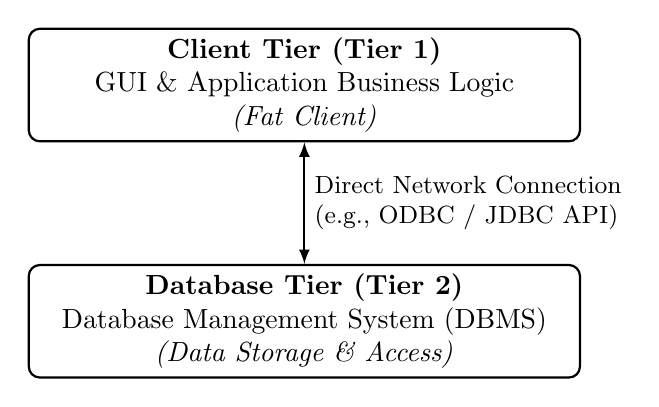
\begin{tikzpicture}[
    thick,
    tier/.style={draw, rounded corners, minimum width=7cm, minimum height=1.4cm, align=center, fill=white, font=\normalsize},
    conn/.style={thick, <->, >=latex}
]
    % Nodes
    \node[tier] (client) at (0, 3) {\textbf{Client Tier (Tier 1)} \\ GUI \& Application Business Logic \\ \textit{(Fat Client)}};
    \node[tier] (db) at (0, 0) {\textbf{Database Tier (Tier 2)} \\ Database Management System (DBMS) \\ \textit{(Data Storage \& Access)}};

    % Connections
    \draw[conn] (client) -- (db) node[midway, right, font=\small, align=left] {Direct Network Connection \\ (e.g., ODBC / JDBC API)};
\end{tikzpicture}
\end{center}
\vspace{1em}

\textbf{Properties \& Characteristics:}
\begin{itemize}
    \item \textbf{Working Principle:} The client application directly establishes a connection to the database server using APIs like ODBC or JDBC. Queries are generated by the client and sent directly to the database.
    \item \textbf{Advantages:} 
        \begin{itemize}
            \item Simple to design, develop, and deploy.
            \item Faster response times for small user groups due to the lack of an intermediate layer.
        \end{itemize}
    \item \textbf{Disadvantages:} 
        \begin{itemize}
            \item \textbf{Scalability Issue:} Performance degrades significantly as the number of concurrent users increases (each requires a dedicated database connection).
            \item \textbf{Security Risk:} The database is directly exposed to client applications.
            \item \textbf{Maintenance:} Application logic changes require updates on every individual client machine.
        \end{itemize}
\end{itemize}

\vspace{1em}
\hrule
\vspace{1em}

\subsection*{2. Three-Tier Database Architecture}

A \textbf{3-tier architecture} decouples the user interface, business logic, and database management into three separate layers. This is the standard architecture for modern web applications.

\vspace{1em}
\begin{center}
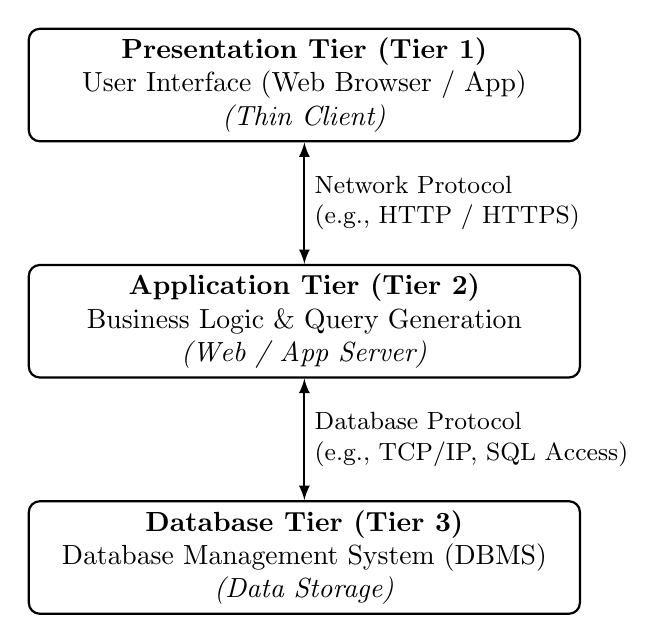
\begin{tikzpicture}[
    thick,
    tier/.style={draw, rounded corners, minimum width=7cm, minimum height=1.4cm, align=center, fill=white, font=\normalsize},
    conn/.style={thick, <->, >=latex}
]
    % Nodes
    \node[tier] (client) at (0, 6) {\textbf{Presentation Tier (Tier 1)} \\ User Interface (Web Browser / App) \\ \textit{(Thin Client)}};
    \node[tier] (app) at (0, 3) {\textbf{Application Tier (Tier 2)} \\ Business Logic \& Query Generation \\ \textit{(Web / App Server)}};
    \node[tier] (db) at (0, 0) {\textbf{Database Tier (Tier 3)} \\ Database Management System (DBMS) \\ \textit{(Data Storage)}};

    % Connections
    \draw[conn] (client) -- (app) node[midway, right, font=\small, align=left] {Network Protocol \\ (e.g., HTTP / HTTPS)};
    \draw[conn] (app) -- (db) node[midway, right, font=\small, align=left] {Database Protocol \\ (e.g., TCP/IP, SQL Access)};
\end{tikzpicture}
\end{center}
\vspace{1em}

\textbf{Properties \& Characteristics:}
\begin{itemize}
    \item \textbf{Working Principle:} The client sends a request to the application server. The application server evaluates the business rules, forms the necessary database queries, executes them against the database server, and finally sends the processed result back to the client.
    \item \textbf{Advantages:} 
        \begin{itemize}
            \item \textbf{High Scalability:} Connection pooling at the application layer allows thousands of clients to share a few database connections.
            \item \textbf{Improved Security:} The database is shielded from direct client access. The application layer acts as a secure gateway.
            \item \textbf{Maintainability:} Business logic updates are made centrally on the application server without altering client software.
        \end{itemize}
    \item \textbf{Disadvantages:} 
        \begin{itemize}
            \item More complex to design, configure, and maintain.
            \item Slight network overhead due to the intermediate routing through the application layer.
        \end{itemize}
\end{itemize}

\vspace{1em}

\subsection*{3. Comparison Summary}

\begin{center}
\renewcommand{\arraystretch}{1.4}
\begin{tabular}{@{} l l l @{}}
\toprule
\textbf{Feature} & \textbf{2-Tier Architecture} & \textbf{3-Tier Architecture} \\
\midrule
\textbf{Client Type} & Fat client (contains application logic) & Thin client (primarily presentation) \\
\textbf{Scalability} & Poor (difficult to scale beyond ~100 users) & Excellent (handles thousands of users) \\
\textbf{Security} & Low (direct database access) & High (database hidden behind app server) \\
\textbf{Maintenance} & High effort (update every client device) & Low effort (centralized updates) \\
\textbf{Use Case} & Legacy desktop software, internal enterprise tools & Web applications, cloud services, e-commerce \\
\bottomrule
\end{tabular}
\end{center}

\end{tcolorbox}

\item Why do we use data abstraction? Describe the different data abstraction levels.
\mk{8} \yr{CSE 215 | L-2/T-1 | 2024--25}

\begin{tcolorbox}[enhanced,breakable,ansbox,colback=cA!4,colframe=cA,boxrule=0.8pt,arc=5pt,title={\textbf{Answer}},fonttitle=\bfseries\color{white},colbacktitle=cA]

\subsection*{1. Definition and Purpose of Data Abstraction}

\textbf{Data Abstraction} is the process of hiding the complex, underlying physical storage details of a database from the end-users and applications, presenting them only with the relevant structural view of the data. 

In a Database Management System (DBMS), highly complex data structures (like B+ trees, hash tables, and linked lists) are used to store and retrieve data efficiently. Because most database users are not trained to interact with such structures, the DBMS implements data abstraction.

\textbf{Why do we use Data Abstraction?}
\begin{itemize}
    \item \textbf{Complexity Hiding:} End-users and application developers can interact with the database without needing to understand disk blocks, byte offsets, or indexing mechanisms.
    \item \textbf{Security \& Authorization:} By restricting what specific users can see (via views), the DBMS prevents unauthorized access to sensitive information.
    \item \textbf{Data Independence:} The ability to change the schema at one level of the database system without having to change the schema at the next higher level.
    \item \textbf{Ease of Access:} It simplifies querying processes by allowing users to use high-level declarative languages like SQL.
\end{itemize}

\vspace{1em}
\subsection*{2. Architecture of Data Abstraction}

Data abstraction is typically implemented using the \textbf{Three-Schema Architecture} (also known as the ANSI/SPARC architecture), which divides the database into three distinct levels.

\vspace{1em}
\begin{center}
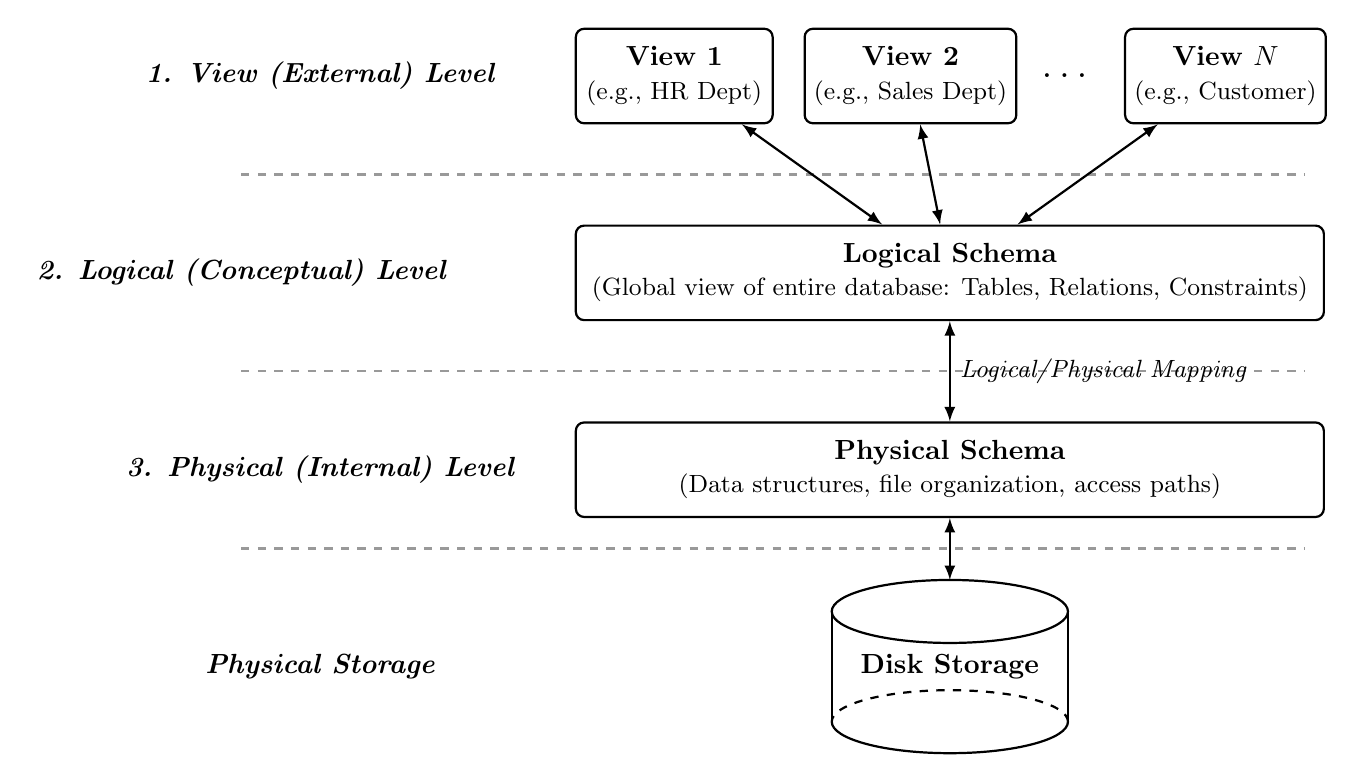
\begin{tikzpicture}[
    thick,
    box/.style={draw, rectangle, rounded corners=3pt, minimum height=1.2cm, align=center, fill=white, font=\bfseries},
    leveltext/.style={font=\bfseries\itshape, align=left}
]
    % Visual separators
    \draw[dashed, gray!80] (-6, 2.75) -- (7.5, 2.75);
    \draw[dashed, gray!80] (-6, 0.25) -- (7.5, 0.25);
    \draw[dashed, gray!80] (-6, -2) -- (7.5, -2);

    % Level Labels
    \node[leveltext] at (-5, 4) {1. View (External) Level};
    \node[leveltext] at (-6, 1.5) {2. Logical (Conceptual) Level};
    \node[leveltext] at (-5, -1) {3. Physical (Internal) Level};
    \node[leveltext] at (-5, -3.5) {Physical Storage};

    % View Level Nodes
    \node[box, minimum width=2.5cm] (v1) at (-0.5, 4) {View 1 \\ \normalfont\small (e.g., HR Dept)};
    \node[box, minimum width=2.5cm] (v2) at (2.5, 4) {View 2 \\ \normalfont\small (e.g., Sales Dept)};
    \node at (4.5, 4) {\Large $\dots$};
    \node[box, minimum width=2.5cm] (vn) at (6.5, 4) {View $N$ \\ \normalfont\small (e.g., Customer)};

    % Logical Level Nodes
    \node[box, minimum width=9.5cm] (log) at (3, 1.5) {Logical Schema \\ \normalfont\small (Global view of entire database: Tables, Relations, Constraints)};

    % Physical Level Nodes
    \node[box, minimum width=9.5cm] (phy) at (3, -1) {Physical Schema \\ \normalfont\small (Data structures, file organization, access paths)};

    % Database (Manual cylinder drawing to ensure no library dependency)
    \draw[thick, fill=white] (3,-2.8) ellipse (1.5cm and 0.4cm);
    \draw[thick] (1.5,-2.8) -- (1.5,-4.2);
    \draw[thick] (4.5,-2.8) -- (4.5,-4.2);
    \draw[thick, fill=white] (1.5,-4.2) arc (180:360:1.5cm and 0.4cm);
    \draw[thick, dashed] (4.5,-4.2) arc (0:180:1.5cm and 0.4cm);
    \node[font=\bfseries, align=center] (db) at (3, -3.5) {Disk Storage};

    % Inter-level Connections (Mappings)
    \draw[<->, thick, >=latex] (v1) -- (log);
    \draw[<->, thick, >=latex] (v2) -- (log);
    \draw[<->, thick, >=latex] (vn) -- (log);
    \draw[<->, thick, >=latex] (log) -- (phy) node[midway, right, font=\small\itshape] {Logical/Physical Mapping};
    \draw[<->, thick, >=latex] (phy) -- (3, -2.4);

\end{tikzpicture}
\end{center}
\vspace{1em}

\subsection*{3. Detailed Description of Abstraction Levels}

\begin{enumerate}
    \item \textbf{Physical (Internal) Level:} 
    \begin{itemize}
        \item \textbf{Definition:} The lowest level of abstraction. It describes \textit{how} the data is actually stored in the underlying storage mediums (HDDs/SSDs).
        \item \textbf{Working Principle:} It defines data structures (like B+ trees, Hash maps), file organizations (sequential, indexed), compression techniques, and encryption. This level is managed by the Database Administrator (DBA).
        \item \textbf{Example:} Storing a `Customer` record as a contiguous block of 256 bytes at a specific memory address, utilizing an ISAM (Indexed Sequential Access Method) index.
    \end{itemize}
    \vspace{0.5em}

    \item \textbf{Logical (Conceptual) Level:}
    \begin{itemize}
        \item \textbf{Definition:} The middle level of abstraction. It describes \textit{what} data is stored in the database and the relationships existing among those data.
        \item \textbf{Working Principle:} It represents the entire database logically. Programmers and DBAs work at this level using Data Definition Language (DDL). There is no hardware awareness at this level.
        \item \textbf{Example:} Defining a relational table `Customer(ID, Name, Account\_Balance)` with a primary key on `ID` and a foreign key linking to a `Transactions` table.
    \end{itemize}
    \vspace{0.5em}

    \item \textbf{View (External) Level:}
    \begin{itemize}
        \item \textbf{Definition:} The highest level of abstraction. It describes only \textit{part} of the entire database.
        \item \textbf{Working Principle:} A database can have multiple views tailored for different user groups. It simplifies interaction by hiding data that is not relevant to the user and masking sensitive information.
        \item \textbf{Example:} A bank teller viewing a customer's `Name` and `Account\_Balance`, while the conceptual level also holds the customer's `Encrypted\_Password` and `SSN`, which the teller is completely unaware of.
    \end{itemize}
\end{enumerate}


\end{tcolorbox}

\item Why does it yield current values when derived attributes are not stored in the database? Discuss with an example.
\mk{10/7} \yr{CSE 215 | L-2/T-1 | 2023--24}\yr{CSE 303 | L-3/T-1 | 2014--15}

\begin{tcolorbox}[enhanced,breakable,ansbox,colback=cA!4,colframe=cA,boxrule=0.8pt,arc=5pt,title={\textbf{Answer}},fonttitle=\bfseries\color{white},colbacktitle=cA]

\subsection*{1. Definition and Concept}

A \textbf{Derived Attribute} is an attribute in a database whose value is not permanently stored in the physical storage. Instead, its value is dynamically calculated (or derived) from one or more related \textbf{base attributes} (which are physically stored) or system functions (such as the current system time) whenever the attribute is queried.

\subsection*{2. Why Derived Attributes Yield Current Values}

Derived attributes yield the most current and accurate values because of their \textbf{on-the-fly computation} mechanism. The underlying reasons include:

\begin{itemize}
    \item \textbf{Runtime Calculation:} The DBMS evaluates the derived value at the exact moment the query is executed. It does not read a stale value from disk.
    \item \textbf{Dependency on Current State:} The derivation formula relies on the present state of the base attributes. If a base attribute changes, the derived attribute instantly reflects this change.
    \item \textbf{Integration with System State:} Many derived attributes depend on the system clock (e.g., \texttt{CURRENT\_DATE}). As time progresses, the calculation naturally factors in the new time, ensuring the result is always up to date.
    \item \textbf{Elimination of Update Anomalies:} If a dynamic value (like age or years of service) were stored statically, a background job would be required to update every record periodically. Skipping this update would lead to stale, incorrect data. Derivation completely avoids this synchronization issue.
\end{itemize}

\subsection*{3. Illustrative Example}

Consider a university database tracking students. 
\begin{itemize}
    \item \textbf{Base Attribute (Stored):} \texttt{Date\_of\_Birth} (e.g., '2002-05-15').
    \item \textbf{Derived Attribute (Not Stored):} \texttt{Age}.
\end{itemize}

If \texttt{Age} were physically stored as `20` in the year 2022, it would become incorrect (stale) by the year 2024. However, by treating \texttt{Age} as a derived attribute, the DBMS computes it dynamically using the formula:
\begin{equation*}
    \text{Age} = \text{Current\_Date} - \text{Date\_of\_Birth}
\end{equation*}
Because \texttt{Current\_Date} advances automatically, executing this query in 2026 will accurately and mathematically yield an age of 24, without a single write operation being made to the database since the student's insertion.

\subsection*{4. ER Diagram Representation}

In an Entity-Relationship (ER) model, derived attributes are denoted by a \textbf{dashed ellipse}. The base attributes are denoted by a standard solid ellipse.

\vspace{1em}
\begin{center}
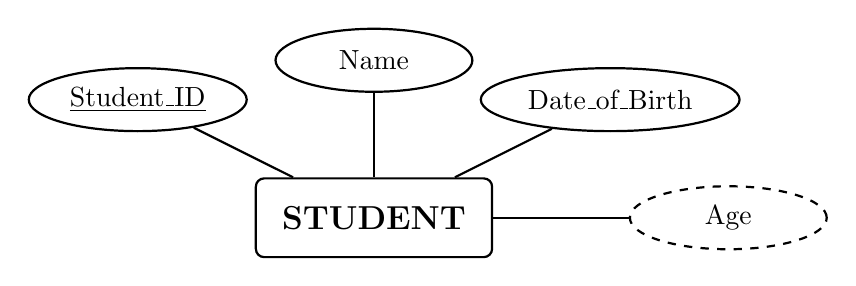
\begin{tikzpicture}[
    thick,
    entity/.style={rectangle, draw, minimum width=3cm, minimum height=1cm, font=\bfseries\large, rounded corners=3pt},
    attribute/.style={ellipse, draw, minimum width=2.5cm, minimum height=0.8cm, font=\normalsize},
    derived/.style={ellipse, draw, dashed, minimum width=2.5cm, minimum height=0.8cm, font=\normalsize}
]
    % Entity
    \node[entity] (student) at (0,0) {STUDENT};
    
    % Attributes
    \node[attribute] (id) at (-3, 1.5) {\underline{Student\_ID}};
    \node[attribute] (name) at (0, 2) {Name};
    \node[attribute] (dob) at (3, 1.5) {Date\_of\_Birth};
    \node[derived] (age) at (4.5, 0) {Age};
    
    % Connections
    \draw (student) -- (id);
    \draw (student) -- (name);
    \draw (student) -- (dob);
    \draw (student) -- (age);
\end{tikzpicture}
\end{center}
\vspace{1em}

\subsection*{5. Implementation (SQL View or Query)}

In standard relational databases, derived attributes are typically implemented using expressions in a \texttt{SELECT} statement or encapsulated within a \textbf{View}.

\begin{lstlisting}[language=SQL]
-- Creating a view to continuously expose the derived 'Age' attribute
CREATE VIEW Student_Current_Profile AS
SELECT 
    Student_ID,
    Name,
    Date_of_Birth,
    -- Derivation calculation happens here on the fly
    FLOOR(DATEDIFF(DAY, Date_of_Birth, CURRENT_DATE) / 365.25) AS Age
FROM 
    STUDENT;
\end{lstlisting}

\subsection*{6. Comparison Summary}

\begin{center}
\renewcommand{\arraystretch}{1.4}
\begin{tabularx}{\textwidth}{@{} l X X @{}}
\toprule
\textbf{Property} & \textbf{Stored Attribute} & \textbf{Derived Attribute} \\
\midrule
\textbf{Storage} & Occupies physical disk space. & Does not occupy disk space. \\
\textbf{Accuracy over time} & Becomes stale if not updated continuously. & Always accurate; dynamically computes current state. \\
\textbf{Performance} & Faster retrieval (simple disk read). & Slower retrieval (requires CPU computation time). \\
\textbf{Redundancy} & Introduces redundancy if logically dependent on other attributes. & Completely eliminates logical redundancy. \\
\bottomrule
\end{tabularx}
\end{center}

\end{tcolorbox}

\item What are the requirements of an ideal DBMS? Define entity and attribute in the context of database with suitable example(s).
\mk{10} \yr{CSE 215 | L-2/T-2 | 2018--19}

\begin{tcolorbox}[enhanced,breakable,ansbox,colback=cA!4,colframe=cA,boxrule=0.8pt,arc=5pt,title={\textbf{Answer}},fonttitle=\bfseries\color{white},colbacktitle=cA]

\subsection*{1. Requirements of an Ideal DBMS}

An ideal Database Management System (DBMS) must provide a robust, secure, and efficient environment for storing and retrieving data. The primary requirements include:

\begin{itemize}
    \item \textbf{Data Integrity and Consistency:} The system must enforce constraints (e.g., primary keys, foreign keys, domain constraints) to ensure data remains accurate and valid across all tables, even after multiple transactions.
    \item \textbf{Concurrency Control:} It must allow multiple users to access and modify data simultaneously without causing data corruption or inconsistencies, typically achieved by enforcing ACID (Atomicity, Consistency, Isolation, Durability) properties.
    \item \textbf{Data Security and Authorization:} The DBMS must restrict unauthorized access, ensuring that only authenticated users with specific privileges can view or manipulate sensitive data.
    \item \textbf{Crash Recovery and Resilience:} In the event of a hardware or software failure, the system must be able to restore the database to a consistent state without losing any committed data.
    \item \textbf{Data Independence:} The architecture should allow changes in the physical storage layer without affecting the logical schema (Physical Data Independence), and changes in the logical schema without rewriting application programs (Logical Data Independence).
    \item \textbf{Performance and Scalability:} It must efficiently process complex queries over massive datasets and scale seamlessly as the volume of data and the number of concurrent users increase.
    \item \textbf{High-Level Query Language:} It should provide a declarative interface (like SQL) allowing users to retrieve data easily without needing to understand complex physical access paths.
\end{itemize}

\vspace{1em}
\hrule
\vspace{1em}

\subsection*{2. Definition of Entity and Attribute}

In the context of database design and the Entity-Relationship (ER) model:

\begin{itemize}
    \item \textbf{Entity:} An entity is a distinguishable real-world object, concept, or event that exists independently and about which data needs to be collected and stored. Entities are mapped to \textbf{Tables} (or relations) in a relational database.
    \item \textbf{Attribute:} An attribute is a characteristic, property, or trait that describes an entity. It holds specific pieces of information about the entity. Attributes are mapped to \textbf{Columns} in a relational database.
\end{itemize}

\subsection*{3. Suitable Example and ER Diagram}

Let us consider a university database environment:
\begin{itemize}
    \item \textbf{Entity:} \texttt{STUDENT} (represents a physical person).
    \item \textbf{Attributes of \texttt{STUDENT}:} 
    \begin{itemize}
        \item \texttt{Student\_ID}: A \textit{key attribute} (uniquely identifies the student).
        \item \texttt{Name}: A \textit{simple attribute}.
        \item \texttt{Phone}: A \textit{multivalued attribute} (a student can have multiple phone numbers).
        \item \texttt{Age}: A \textit{derived attribute} (calculated from Date of Birth).
    \end{itemize}
\end{itemize}

The following ER Diagram visually represents the \texttt{STUDENT} entity and its associated attributes based on standard ER notation:

\vspace{1.5em}
\begin{center}
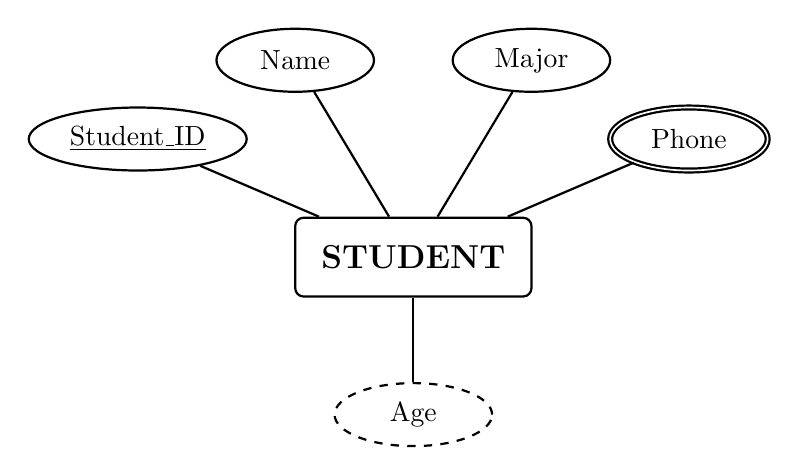
\begin{tikzpicture}[
    thick,
    entity/.style={rectangle, draw, minimum width=3cm, minimum height=1cm, font=\bfseries\large, rounded corners=3pt},
    attribute/.style={ellipse, draw, minimum width=2cm, minimum height=0.8cm, font=\normalsize, align=center},
    multi/.style={ellipse, draw, double, minimum width=2cm, minimum height=0.8cm, font=\normalsize, align=center},
    derived/.style={ellipse, draw, dashed, minimum width=2cm, minimum height=0.8cm, font=\normalsize, align=center}
]
    % Central Entity
    \node[entity] (student) at (0,0) {STUDENT};
    
    % Attributes Nodes
    \node[attribute] (id) at (-3.5, 1.5) {\underline{Student\_ID}};
    \node[attribute] (name) at (-1.5, 2.5) {Name};
    \node[attribute] (major) at (1.5, 2.5) {Major};
    \node[multi] (phone) at (3.5, 1.5) {Phone};
    \node[derived] (age) at (0, -2) {Age};
    
    % Connection Lines
    \draw (student) -- (id);
    \draw (student) -- (name);
    \draw (student) -- (major);
    \draw (student) -- (phone);
    \draw (student) -- (age);
\end{tikzpicture}
\end{center}
\vspace{1.5em}

\subsection*{4. Comparison Table (Entity vs. Attribute)}

\begin{center}
\renewcommand{\arraystretch}{1.4}
\begin{tabularx}{0.95\textwidth}{@{} >{\bfseries}l X X @{}}
\toprule
Feature & Entity & Attribute \\
\midrule
\textbf{Definition} & A distinct real-world object or concept. & A property or characteristic describing an object. \\
\textbf{Relational Mapping} & Becomes a \textbf{Table}. & Becomes a \textbf{Column} in that table. \\
\textbf{ER Diagram Notation} & Represented by a \textbf{Rectangle}. & Represented by an \textbf{Ellipse}. \\
\textbf{Example} & `Car`, `Employee`, `Order` & `Color`, `Salary`, `Order\_Date` \\
\bottomrule
\end{tabularx}
\end{center}


\end{tcolorbox}

%% Q9 — 2018-19
\item What are bags in DBMS? How are they different from sets? Give examples of union, intersection and minus operation on bags to highlight the differences.
\mk{15} \yr{CSE 303 | L-3/T-1 | 2012--13}

\begin{tcolorbox}[enhanced,breakable,ansbox,colback=cA!4,colframe=cA,boxrule=0.8pt,arc=5pt,title={\textbf{Answer}},fonttitle=\bfseries\color{white},colbacktitle=cA]

\subsection*{1. Definition of Bags (Multisets) in DBMS}

In the context of a Database Management System (DBMS), a \textbf{bag} (also known as a \textbf{multiset}) is an unordered collection of elements where \textbf{duplicate elements are permitted}. 

While pure relational algebra is mathematically based on set theory (where duplicates are strictly prohibited), commercial database systems (like SQL) inherently operate on bags by default. This is because eliminating duplicates is a computationally expensive operation (requiring sorting or hashing). Therefore, unless a user explicitly requests duplicate removal (e.g., using the \texttt{DISTINCT} keyword), a DBMS will output a bag of tuples.

\subsection*{2. Difference Between Bags and Sets}

\begin{itemize}
    \item \textbf{Sets:} A set contains distinct elements. An element $x$ either belongs to a set $S$ or it does not. The cardinality (count) of any element in a set is at most $1$.
    \item \textbf{Bags:} A bag can contain multiple identical copies of the same element. An element $x$ belongs to a bag $B$ with a specific count or frequency, denoted as $C(x, B) \geq 0$.
\end{itemize}

\vspace{1em}
\begin{center}
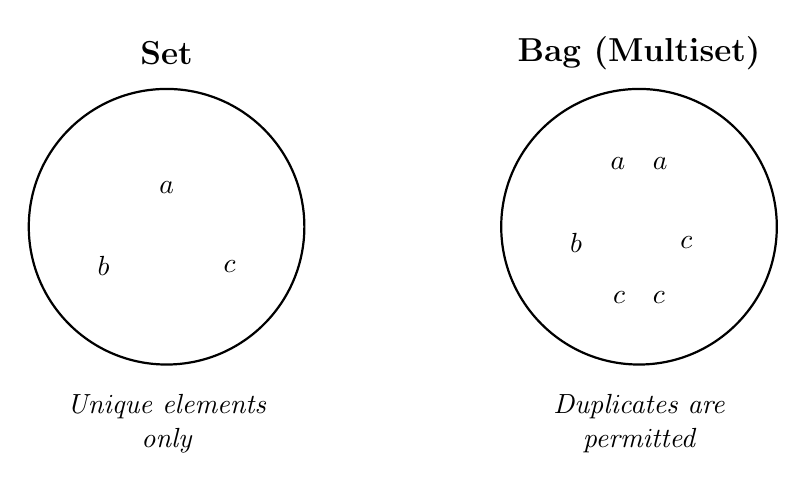
\begin{tikzpicture}[
    thick,
    container/.style={circle, draw, minimum size=3.5cm, fill=white},
    label/.style={font=\bfseries\large}
]
    % Set Representation
    \node[container] (set) at (0,0) {};
    \node[label] at (0, 2.2) {Set};
    \node at (0, 0.5) {$a$};
    \node at (-0.8, -0.5) {$b$};
    \node at (0.8, -0.5) {$c$};
    \node[font=\itshape, align=center] at (0, -2.5) {Unique elements\\only};

    % Bag Representation
    \node[container] (bag) at (6,0) {};
    \node[label] at (6, 2.2) {Bag (Multiset)};
    \node at (6, 0.8) {$a \quad a$};
    \node at (5.2, -0.2) {$b$};
    \node at (6.6, -0.2) {$c$};
    \node at (6, -0.9) {$c \quad c$};
    \node[font=\itshape, align=center] at (6, -2.5) {Duplicates are\\permitted};
\end{tikzpicture}
\end{center}
\vspace{1em}

\subsection*{3. Operations on Bags vs. Sets}

Let $C(x, A)$ represent the number of occurrences of an element $x$ in a bag $A$.
Consider two bags:
\begin{itemize}
    \item Bag $A = \{a, a, a, b, b, c\}$
    \item Bag $B = \{a, a, b, b, b, d\}$
\end{itemize}
Therefore, element counts are: 
$C(a, A) = 3$, $C(b, A) = 2$, $C(c, A) = 1$; and $C(a, B) = 2$, $C(b, B) = 3$, $C(d, B) = 1$.

\subsubsection*{A. Bag Union ($\cup$)}
In a bag union, the count of an element in the result is the \textbf{sum} of its counts in the two bags.
$$C(x, A \cup B) = C(x, A) + C(x, B)$$
\begin{itemize}
    \item \textbf{Bag Result:} $A \cup B = \{a, a, a, a, a, b, b, b, b, b, c, d\}$
    \item \textbf{Comparison to Set Union:} A strict set union of $A$ and $B$ would simply be $\{a, b, c, d\}$, completely ignoring frequencies.
\end{itemize}

\subsubsection*{B. Bag Intersection ($\cap$)}
In a bag intersection, the count of an element in the result is the \textbf{minimum} of its counts in the two bags.
$$C(x, A \cap B) = \min(C(x, A), C(x, B))$$
\begin{itemize}
    \item \textbf{Bag Result:} $A \cap B = \{a, a, b, b\}$
    \item \textit{Explanation:} $a$ appears three times in $A$ and two times in $B$; the minimum is two. $b$ appears twice in $A$ and three times in $B$; the minimum is two. $c$ and $d$ do not appear in both, so their minimum count is zero.
\end{itemize}

\subsubsection*{C. Bag Difference / Minus ($-$)}
In a bag difference, the count of an element in the result is the count in the first bag \textbf{minus} the count in the second bag, floored at zero (an element cannot have a negative count).
$$C(x, A - B) = \max(0, C(x, A) - C(x, B))$$
\begin{itemize}
    \item \textbf{Bag Result:} $A - B = \{a, c\}$
    \item \textit{Explanation:} For $a$: $\max(0, 3 - 2) = 1$. For $b$: $\max(0, 2 - 3) = 0$. For $c$: $\max(0, 1 - 0) = 1$. 
\end{itemize}

\subsection*{4. Comparison Summary Table}

\begin{center}
\renewcommand{\arraystretch}{1.4}
\begin{tabularx}{\textwidth}{@{} >{\bfseries}l X X @{}}
\toprule
Feature & Set Semantics & Bag (Multiset) Semantics \\
\midrule
\textbf{Duplicates} & Strictly not allowed. & Allowed and maintained. \\
\textbf{Union ($A \cup B$)} & Element exists if it is in $A$ or $B$. & Sum of occurrences: $C(A) + C(B)$. \\
\textbf{Intersection ($A \cap B$)} & Element exists if it is in both $A$ and $B$. & Minimum of occurrences: $\min(C(A), C(B))$. \\
\textbf{Difference ($A - B$)} & Element exists if it is in $A$ but not $B$. & Remaining occurrences: $\max(0, C(A) - C(B))$. \\
\textbf{Performance} & Slower (requires duplicate elimination). & Faster (simply streams tuples). \\
\bottomrule
\end{tabularx}
\end{center}

\end{tcolorbox}

%% Q8
\item What are the key properties of a DBMS?
\mk{8} \yr{CSE 303 | L-3/T-1 | 2011--12}

\begin{tcolorbox}[enhanced,breakable,ansbox,colback=cA!4,colframe=cA,boxrule=0.8pt,arc=5pt,title={\textbf{Answer}},fonttitle=\bfseries\color{white},colbacktitle=cA]

\subsection*{1. Introduction}
A Database Management System (DBMS) is designed to manage large bodies of information efficiently and securely. To achieve this, it possesses several key properties that distinguish it from traditional file-processing systems, making it the standard for modern data management.

\subsection*{2. Fundamental Properties of a DBMS}

\begin{itemize}
    \item \textbf{Control of Data Redundancy:} Unlike flat-file systems where duplicate data is scattered across multiple locations, a DBMS integrates data into a central repository, minimizing duplication and preventing data inconsistency.
    \item \textbf{Data Security and Authorization:} A DBMS enforces security by ensuring that only authorized users can access or modify the data. It supports the creation of user accounts, roles, and granular access privilege configurations.
    \item \textbf{Data Independence:} The architecture provides a strict separation between application programs and the physical data storage. 
    \begin{itemize}
        \item \textit{Logical Data Independence:} The ability to change the conceptual schema without altering application programs.
        \item \textit{Physical Data Independence:} The ability to change the underlying storage structure without altering the conceptual schema.
    \end{itemize}
    \item \textbf{Concurrency Control:} When multiple users or programs attempt to access the same data simultaneously, the DBMS systematically manages these interactions (usually via locking mechanisms) to prevent data corruption.
    \item \textbf{Backup and Recovery:} A DBMS provides robust, automatic mechanisms to back up data and recover it to a consistent state in the event of hardware crashes or software failures.
    \item \textbf{Data Integrity:} The system enforces structural rules and constraints (such as primary keys, foreign keys, and domain constraints) to ensure all data stored is structurally accurate and functionally valid.
\end{itemize}

\subsection*{3. Transaction Properties (ACID)}
At the core of a robust relational DBMS is its ability to process database transactions reliably. These required transactional properties are summarized by the \textbf{ACID} acronym:

\begin{enumerate}
    \item \textbf{Atomicity:} Often called the "all-or-nothing" rule. A transaction is treated as a single indivisible logical unit of work; either all its operations are executed successfully, or none are.
    \item \textbf{Consistency:} A transaction must reliably transition the database from one valid, consistent state to another, strictly adhering to all defined database rules and constraints.
    \item \textbf{Isolation:} Concurrent transactions execute completely independent of one another. Intermediate, uncommitted states of one transaction are invisible to other concurrent transactions.
    \item \textbf{Durability:} Once a transaction is successfully committed, its changes are permanently recorded in non-volatile storage and will survive any subsequent system failures or power losses.
\end{enumerate}

\subsection*{4. Visual Summary of Key Properties}

\vspace{1.5em}
\begin{center}
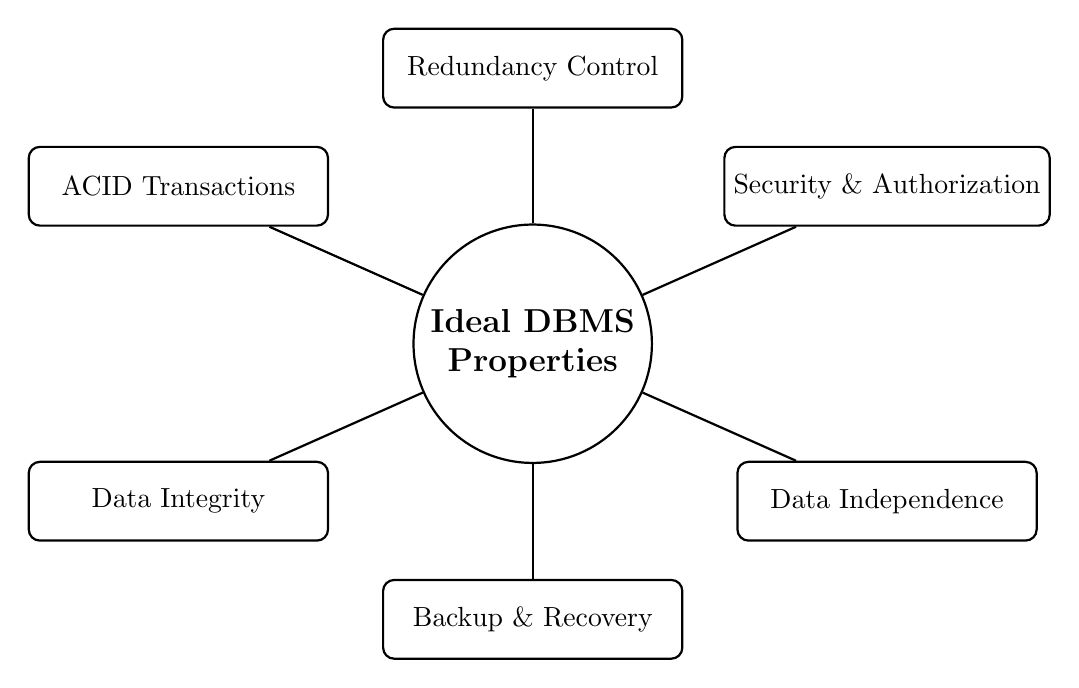
\begin{tikzpicture}[
    thick,
    centerNode/.style={circle, draw, minimum size=2.8cm, font=\bfseries\large, align=center},
    propNode/.style={rectangle, draw, rounded corners=4pt, minimum width=3.8cm, minimum height=1cm, font=\normalsize, align=center, fill=white}
]
    % Central Node
    \node[centerNode] (dbms) at (0,0) {Ideal DBMS\\Properties};

    % Surrounding Nodes
    \node[propNode] (red) at (0, 3.5) {Redundancy Control};
    \node[propNode] (sec) at (4.5, 2) {Security \& Authorization};
    \node[propNode] (ind) at (4.5, -2) {Data Independence};
    \node[propNode] (rec) at (0, -3.5) {Backup \& Recovery};
    \node[propNode] (int) at (-4.5, -2) {Data Integrity};
    \node[propNode] (acid) at (-4.5, 2) {ACID Transactions};

    % Connecting lines
    \draw (dbms) -- (red);
    \draw (dbms) -- (sec);
    \draw (dbms) -- (ind);
    \draw (dbms) -- (rec);
    \draw (dbms) -- (int);
    \draw (dbms) -- (acid);

\end{tikzpicture}
\end{center}
\vspace{1.5em}


\end{tcolorbox}

%% Q6
\item Show the major components and their interactions in a DBMS. Briefly explain the functionalities of major components.
\mk{15} \yr{CSE 303 | L-3/T-1 | 2011--12}

\begin{tcolorbox}[enhanced,breakable,ansbox,colback=cA!4,colframe=cA,boxrule=0.8pt,arc=5pt,title={\textbf{Answer}},fonttitle=\bfseries\color{white},colbacktitle=cA]

\subsection*{1. DBMS Architecture and Component Interactions}

A Database Management System (DBMS) is highly complex and is divided into multiple modular components that interact to execute queries, manage storage, and ensure data integrity. The architecture is broadly categorized into the \textbf{Query Processor}, the \textbf{Storage Manager}, and the \textbf{Disk Storage}.

The diagram below illustrates the major components and the flow of instructions (interactions) from the user level down to the physical disk.

\vspace{1.5em}
\begin{center}
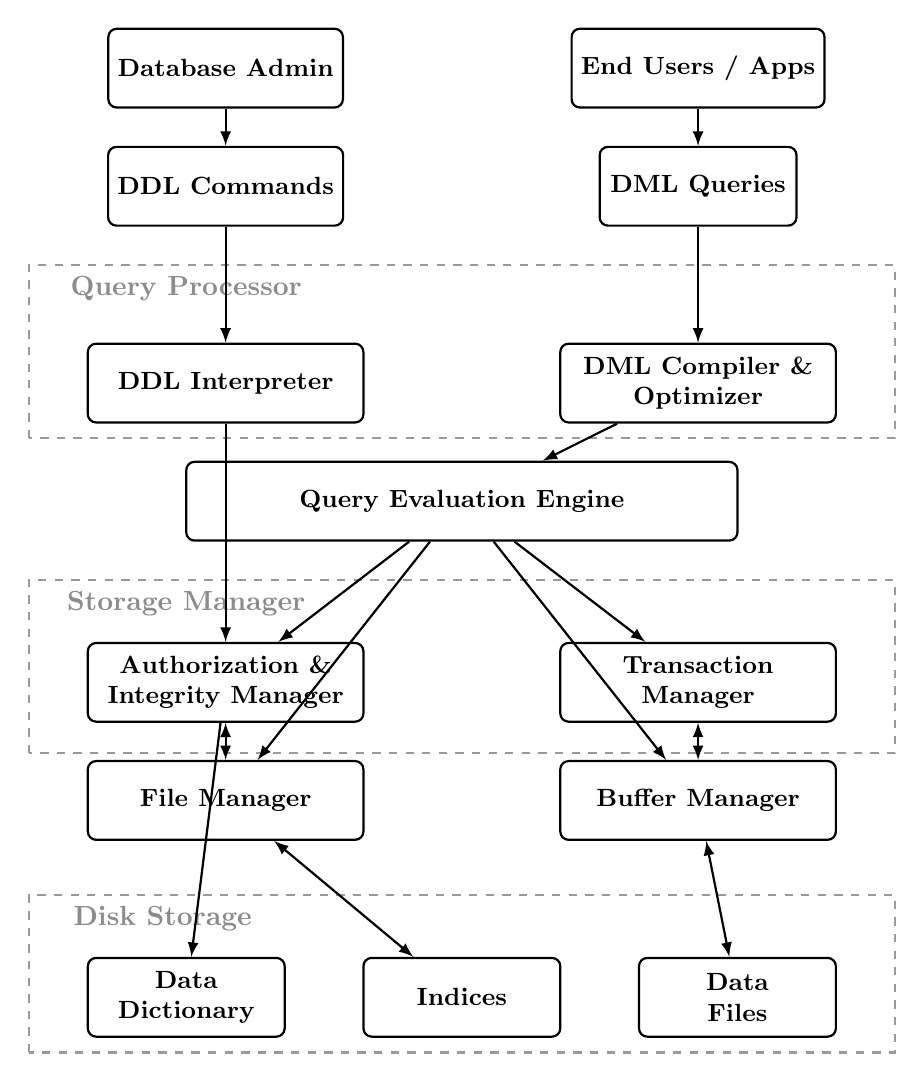
\begin{tikzpicture}[
    thick,
    box/.style={draw, rectangle, rounded corners=3pt, minimum width=3.5cm, minimum height=1cm, align=center, fill=white, font=\small\bfseries},
    groupbox/.style={draw, rectangle, dashed, inner sep=10pt},
    arrow/.style={->, >=latex, thick},
    textlabel/.style={font=\footnotesize\itshape}
]
    % --- Users ---
    \node[box, minimum width=2.5cm] (dba) at (-3, 9) {Database Admin};
    \node[box, minimum width=2.5cm] (user) at (3, 9) {End Users / Apps};

    % --- Interfaces ---
    \node[box, minimum width=2.5cm] (ddl_cmd) at (-3, 7.5) {DDL Commands};
    \node[box, minimum width=2.5cm] (dml_cmd) at (3, 7.5) {DML Queries};

    \draw[arrow] (dba) -- (ddl_cmd);
    \draw[arrow] (user) -- (dml_cmd);

    % --- Query Processor ---
    \draw[dashed, gray!80] (-5.5, 4.3) rectangle (5.5, 6.5);
    \node[font=\bfseries, text=gray!90] at (-3.5, 6.2) {Query Processor};

    \node[box] (ddl_interp) at (-3, 5) {DDL Interpreter};
    \node[box] (dml_comp) at (3, 5) {DML Compiler \& \\ Optimizer};
    \node[box, minimum width=7cm] (query_eval) at (0, 3.5) {Query Evaluation Engine};

    \draw[arrow] (ddl_cmd) -- (ddl_interp);
    \draw[arrow] (dml_cmd) -- (dml_comp);
    \draw[arrow] (dml_comp) -- (query_eval);

    % --- Storage Manager ---
    \draw[dashed, gray!80] (-5.5, 0.3) rectangle (5.5, 2.5);
    \node[font=\bfseries, text=gray!90] at (-3.5, 2.2) {Storage Manager};

    \node[box] (auth) at (-3, 1.2) {Authorization \& \\ Integrity Manager};
    \node[box] (trans) at (3, 1.2) {Transaction \\ Manager};
    \node[box] (file) at (-3, -0.3) {File Manager};
    \node[box] (buffer) at (3, -0.3) {Buffer Manager};

    % Interactions from Query Processor to Storage Manager
    \draw[arrow] (ddl_interp) -- (auth);
    \draw[arrow] (query_eval) -- (auth);
    \draw[arrow] (query_eval) -- (trans);
    \draw[arrow] (query_eval) -- (file);
    \draw[arrow] (query_eval) -- (buffer);
    
    % Internal SM links
    \draw[<->, >=latex, thick] (auth) -- (file);
    \draw[<->, >=latex, thick] (trans) -- (buffer);

    % --- Disk Storage ---
    \draw[dashed, gray!80] (-5.5, -3.5) rectangle (5.5, -1.5);
    \node[font=\bfseries, text=gray!90] at (-3.8, -1.8) {Disk Storage};

    \node[box, minimum width=2.5cm] (dict) at (-3.5, -2.8) {Data \\ Dictionary};
    \node[box, minimum width=2.5cm] (indices) at (0, -2.8) {Indices};
    \node[box, minimum width=2.5cm] (data) at (3.5, -2.8) {Data \\ Files};

    % Interactions from Storage Manager to Disk
    \draw[arrow] (auth) -- (dict);
    \draw[<->, >=latex, thick] (file) -- (indices);
    \draw[<->, >=latex, thick] (buffer) -- (data);

\end{tikzpicture}
\end{center}
\vspace{1em}

\subsection*{2. Functionalities of Major Components}

The DBMS is divided into three primary functional blocks:

\subsubsection*{A. Query Processor}
The query processor handles incoming queries, translates them into low-level instructions, and optimizes them for performance.
\begin{itemize}
    \item \textbf{DDL Interpreter:} Parses Data Definition Language (DDL) statements (like \texttt{CREATE TABLE}) and records the definitions in the data dictionary.
    \item \textbf{DML Compiler and Query Optimizer:} Translates Data Manipulation Language (DML) statements (like \texttt{SELECT}, \texttt{UPDATE}) into an execution plan. The optimizer evaluates various execution strategies and selects the most efficient one based on cost (CPU, I/O).
    \item \textbf{Query Evaluation Engine:} Executes the low-level instructions generated by the DML compiler, coordinating with the storage manager to retrieve the required records.
\end{itemize}

\subsubsection*{B. Storage Manager}
The storage manager acts as the interface between the low-level data on the disk and the application queries. It is responsible for efficient storage, retrieval, and updating of data.
\begin{itemize}
    \item \textbf{Authorization and Integrity Manager:} Verifies that the user issuing the query has the correct permissions and ensures that the operation does not violate any database constraints (e.g., primary/foreign keys).
    \item \textbf{Transaction Manager:} Ensures that the database remains in a consistent state despite system failures. It controls concurrent access, ensuring transactions adhere to ACID properties.
    \item \textbf{File Manager:} Manages the allocation of space on disk storage and the data structures used to represent information stored on disk.
    \item \textbf{Buffer Manager:} Responsible for fetching data from disk storage into main memory (RAM) and deciding what data to cache to minimize expensive disk I/O operations.
\end{itemize}

\subsubsection*{C. Disk Storage (Data Structures)}
This represents the physical layer where the information is permanently written.
\begin{itemize}
    \item \textbf{Data Files:} The actual files residing on the disk that store the database records.
    \item \textbf{Data Dictionary (Metadata):} Stores data about the data, including table schemas, constraints, user permissions, and statistical data used by the query optimizer.
    \item \textbf{Indices:} Auxiliary data structures (such as B+ Trees or Hash tables) that provide fast access to data items based on key values, bypassing sequential scans.
\end{itemize}


\end{tcolorbox}

%% Q7
\item Describe the key properties that give a DBMS edge over a file system.
\mk{14} \yr{CSE 303 | L-3/T-1 | 2010--11}

\begin{tcolorbox}[enhanced,breakable,ansbox,colback=cA!4,colframe=cA,boxrule=0.8pt,arc=5pt,title={\textbf{Answer}},fonttitle=\bfseries\color{white},colbacktitle=cA]

\subsection*{1. Introduction}
Before the advent of Database Management Systems (DBMS), data was stored using traditional file-processing systems where each application maintained its own set of files. This approach led to severe limitations as data grew in size and complexity. A DBMS provides a centralized, robust architecture that overcomes these limitations, offering significant advantages in data handling, security, and performance.

\subsection*{2. Visual Comparison: Architecture}

\vspace{1.5em}
\begin{center}
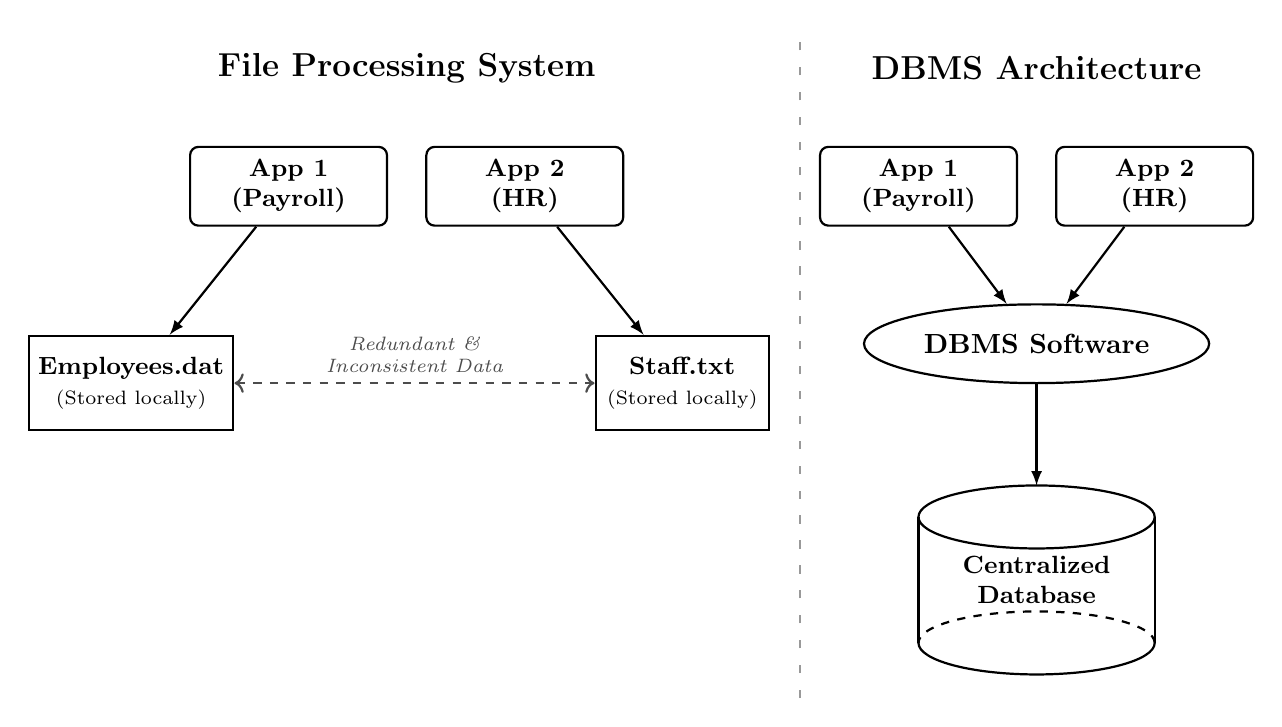
\begin{tikzpicture}[
    thick,
    app/.style={draw, rectangle, rounded corners=3pt, minimum width=2.5cm, minimum height=1cm, align=center, fill=white, font=\small\bfseries},
    dbms/.style={draw, ellipse, minimum width=3cm, minimum height=1cm, align=center, fill=white, font=\bfseries},
    file/.style={draw, rectangle, minimum width=2.2cm, minimum height=1.2cm, align=center, fill=white, font=\small\bfseries},
    arrow/.style={->, >=latex, thick}
]
    % --- File System Side (Left) ---
    \node[font=\bfseries\large] at (-4, 5.5) {File Processing System};
    
    \node[app] (app1) at (-5.5, 4) {App 1 \\ (Payroll)};
    \node[app] (app2) at (-2.5, 4) {App 2 \\ (HR)};
    
    \node[file] (f1) at (-7.5, 1.5) {Employees.dat \\ \normalfont\scriptsize (Stored locally)};
    \node[file] (f2) at (-0.5, 1.5) {Staff.txt \\ \normalfont\scriptsize (Stored locally)};
    
    \draw[arrow] (app1) -- (f1);
    \draw[arrow] (app2) -- (f2);
    
    \draw[<->, dashed, thick, color=black!70] (f1) -- (f2) node[midway, above, font=\scriptsize\itshape, align=center] {Redundant \& \\ Inconsistent Data};

    % --- DBMS Side (Right) ---
    \node[font=\bfseries\large] at (4, 5.5) {DBMS Architecture};
    
    \node[app] (app3) at (2.5, 4) {App 1 \\ (Payroll)};
    \node[app] (app4) at (5.5, 4) {App 2 \\ (HR)};
    
    \node[dbms] (dbms_node) at (4, 2) {DBMS Software};
    
    % Central Database (Manual cylinder drawing)
    \draw[thick, fill=white] (4, -0.2) ellipse (1.5cm and 0.4cm);
    \draw[thick] (2.5, -0.2) -- (2.5, -1.8);
    \draw[thick] (5.5, -0.2) -- (5.5, -1.8);
    \draw[thick, fill=white] (2.5, -1.8) arc (180:360:1.5cm and 0.4cm);
    \draw[thick, dashed] (5.5, -1.8) arc (0:180:1.5cm and 0.4cm);
    \node[font=\small\bfseries, align=center] (db_node) at (4, -1) {Centralized \\ Database};

    \draw[arrow] (app3) -- (dbms_node);
    \draw[arrow] (app4) -- (dbms_node);
    \draw[arrow] (dbms_node) -- (4, 0.2);

    % --- Separator ---
    \draw[loosely dashed, gray!80] (1, -2.5) -- (1, 6);
\end{tikzpicture}
\end{center}
\vspace{1.5em}

\subsection*{3. Key Properties That Give DBMS an Edge}

The decisive edge of a DBMS over file-based systems stems from the following core properties:

\begin{enumerate}
    \item \textbf{Data Abstraction and Independence:}
    \begin{itemize}
        \item \textit{File System:} Application code is tightly coupled to the physical structure of the files. Adding a new field to a text file requires rewriting every application that reads it.
        \item \textit{DBMS:} Provides logical and physical \textbf{data independence}. Users interact with a logical view of the data. The underlying storage mechanisms (like switching from HDDs to SSDs or altering indexing methods) can change without impacting the application code.
    \end{itemize}
    \vspace{0.5em}

    \item \textbf{Control of Data Redundancy and Inconsistency:}
    \begin{itemize}
        \item \textit{File System:} Data is fragmented across multiple departments, leading to massive duplication (redundancy). If an employee's address changes, it might be updated in the Payroll file but forgotten in the HR file (inconsistency).
        \item \textit{DBMS:} Integrates and centralizes data via \textbf{normalization}. Duplication is minimized, ensuring that a single update reflects universally, maintaining global data consistency.
    \end{itemize}
    \vspace{0.5em}

    \item \textbf{High-Level Data Access (Query Languages):}
    \begin{itemize}
        \item \textit{File System:} Extracting specific data requires writing custom procedural scripts (e.g., writing a Python script to parse a CSV and filter records).
        \item \textit{DBMS:} Offers declarative query languages like \textbf{SQL}. A user merely describes \textit{what} data is needed (e.g., \texttt{SELECT * FROM Employees WHERE Salary > 50000}), and the DBMS optimizer dynamically determines the most efficient way to fetch it using built-in access paths and indices.
    \end{itemize}
    \vspace{0.5em}

    \item \textbf{Enforcement of Data Integrity:}
    \begin{itemize}
        \item \textit{File System:} Integrity constraints (e.g., "Age must be $>18$" or "Department ID must exist") must be manually coded into every single application.
        \item \textit{DBMS:} Constraints (Primary Keys, Foreign Keys, Domain constraints) are centralized within the database schema. The DBMS strictly rejects any transaction that violates these rules, guaranteeing valid data.
    \end{itemize}
    \vspace{0.5em}

    \item \textbf{Concurrency Control and ACID Transactions:}
    \begin{itemize}
        \item \textit{File System:} Employs coarse-grained locking. If one user opens a file to edit a single line, the entire file is often locked, preventing concurrent access by others.
        \item \textit{DBMS:} Provides fine-grained (row-level) locking and guarantees \textbf{ACID} (Atomicity, Consistency, Isolation, Durability) properties. Thousands of users can read and write simultaneously without interfering with each other (Isolation), and transactions are treated as indivisible units of work (Atomicity).
    \end{itemize}
    \vspace{0.5em}

    \item \textbf{Crash Recovery (Durability):}
    \begin{itemize}
        \item \textit{File System:} A power failure mid-write can corrupt the file, requiring manual restoration from a backup.
        \item \textit{DBMS:} Uses Write-Ahead Logging (WAL) and undo/redo mechanisms. If a crash occurs, the DBMS automatically recovers, rolling back incomplete transactions to ensure the database remains in a consistent state.
    \end{itemize}
\end{enumerate}

\subsection*{4. Comparison Summary}

\begin{center}
\renewcommand{\arraystretch}{1.5}
\begin{tabularx}{\textwidth}{@{} >{\bfseries}l X X @{}}
\toprule
Feature & Traditional File System & DBMS \\
\midrule
Data Redundancy & Very high (scattered duplicate data). & Minimized (centralized and normalized). \\
Data Independence & Low (applications depend on file structures). & High (abstracts physical storage). \\
Querying & Difficult (requires custom procedural code). & Easy (declarative languages like SQL). \\
Concurrency & Poor (file-level locking limits multi-user access). & Excellent (row-level locking and isolation protocols). \\
Data Integrity & Hard-coded in external applications. & Centralized enforcement via schema constraints. \\
Security & Coarse OS-level permissions (Read/Write file). & Granular role-based access control (RBAC). \\
\bottomrule
\end{tabularx}
\end{center}


\end{tcolorbox}

%% Q2
\item Show the block diagram of database management system components.
\mk{14} \yr{CSE 303 | L-3/T-1 | 2010--11}

\begin{tcolorbox}[enhanced,breakable,ansbox,colback=cA!4,colframe=cA,boxrule=0.8pt,arc=5pt,title={\textbf{Answer}},fonttitle=\bfseries\color{white},colbacktitle=cA]

\subsection*{1. Overview of DBMS Architecture}

A Database Management System (DBMS) is a complex software system tasked with managing, storing, and retrieving data efficiently and securely. To handle these responsibilities, the architecture of a DBMS is partitioned into distinct functional modules. The overall block diagram is primarily divided into three major layers:
\begin{itemize}
    \item \textbf{Users and Interfaces:} The top layer where various users interact with the system.
    \item \textbf{Query Processor:} The brain of the DBMS that translates high-level user queries into low-level execution plans.
    \item \textbf{Storage Manager:} The interface between the query processor and the physical disk storage, responsible for efficient data handling and concurrency.
\end{itemize}

\subsection*{2. DBMS Block Diagram}

\vspace{1em}
\begin{center}
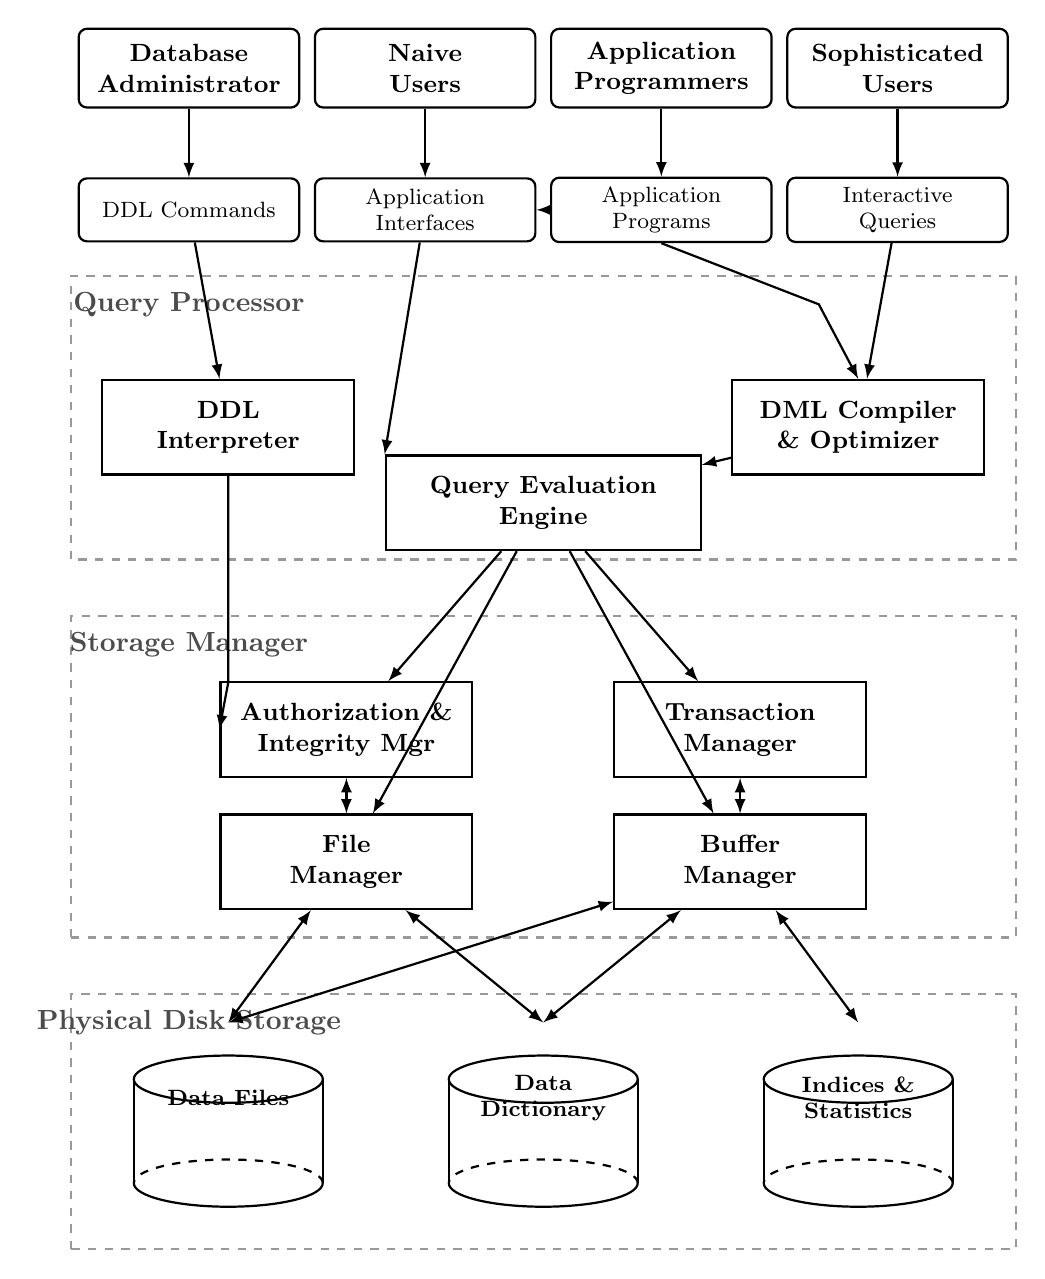
\begin{tikzpicture}[
    thick,y=1.2cm, 
    userbox/.style={draw, rectangle, rounded corners=3pt, minimum width=2.8cm, minimum height=1cm, align=center, fill=white, font=\small\bfseries},
    processbox/.style={draw, rectangle, minimum width=3.2cm, minimum height=1.2cm, align=center, fill=white, font=\small\bfseries},
    diskbox/.style={draw, cylinder, shape border rotate=90, aspect=0.25, minimum width=2.2cm, minimum height=1.5cm, align=center, fill=white, font=\footnotesize\bfseries},
    groupbox/.style={draw, rectangle, dashed, gray!80, inner sep=10pt},
    arrow/.style={->, >=latex, thick},
    darrow/.style={<->, >=latex, thick},
    label/.style={font=\bfseries\color{black!70}}
]

    % ================= USERS AND INTERFACES =================
    \node[userbox] (dba) at (-4.5, 9) {Database \\ Administrator};
    \node[userbox] (naive) at (-1.5, 9) {Naive \\ Users};
    \node[userbox] (app_prog) at (1.5, 9) {Application \\ Programmers};
    \node[userbox] (soph) at (4.5, 9) {Sophisticated \\ Users};

    \node[userbox, minimum height=0.8cm, font=\footnotesize] (ddl_cmd) at (-4.5, 7.5) {DDL Commands};
    \node[userbox, minimum height=0.8cm, font=\footnotesize] (app_int) at (-1.5, 7.5) {Application \\ Interfaces};
    \node[userbox, minimum height=0.8cm, font=\footnotesize] (app_pgms) at (1.5, 7.5) {Application \\ Programs};
    \node[userbox, minimum height=0.8cm, font=\footnotesize] (dml_qry) at (4.5, 7.5) {Interactive \\ Queries};

    \draw[arrow] (dba) -- (ddl_cmd);
    \draw[arrow] (naive) -- (app_int);
    \draw[arrow] (app_prog) -- (app_pgms);
    \draw[arrow] (soph) -- (dml_qry);

    \draw[arrow] (app_pgms) -- (app_int);

    % ================= QUERY PROCESSOR =================
    \draw[dashed, gray!80] (-6, 3.8) rectangle (6, 6.8);
    \node[label] at (-4.5, 6.5) {Query Processor};

    \node[processbox] (ddl_interp) at (-4, 5.2) {DDL \\ Interpreter};
    \node[processbox] (dml_comp) at (4, 5.2) {DML Compiler \\ \& Optimizer};
    \node[processbox, minimum width=4cm] (query_eval) at (0, 4.4) {Query Evaluation \\ Engine};

    \draw[arrow] (ddl_cmd) -- (ddl_interp);
    \draw[arrow] (app_int) -- (query_eval.north west);
    \draw[arrow] (dml_qry) -- (dml_comp);
    \draw[arrow] (app_pgms.south) -- (3.5, 6.5) -- (dml_comp.north);

    \draw[arrow] (dml_comp) -- (query_eval);

    % ================= STORAGE MANAGER =================
    \draw[dashed, gray!80] (-6, -0.2) rectangle (6, 3.2);
    \node[label] at (-4.5, 2.9) {Storage Manager};

    \node[processbox] (auth) at (-2.5, 2) {Authorization \& \\ Integrity Mgr};
    \node[processbox] (trans) at (2.5, 2) {Transaction \\ Manager};
    \node[processbox] (file) at (-2.5, 0.6) {File \\ Manager};
    \node[processbox] (buffer) at (2.5, 0.6) {Buffer \\ Manager};

    % Connections from Query Eval Engine
    \draw[arrow] (query_eval) -- (auth);
    \draw[arrow] (query_eval) -- (trans);
    \draw[arrow] (query_eval) -- (file);
    \draw[arrow] (query_eval) -- (buffer);
    \draw[arrow] (ddl_interp.south) -- (-4, 2.5) -- (auth.west);

    % Internal SM links
    \draw[darrow] (auth) -- (file);
    \draw[darrow] (trans) -- (buffer);

    % ================= DISK STORAGE =================
    \draw[dashed, gray!80] (-6, -3.5) rectangle (6, -0.8);
    \node[label] at (-4.5, -1.1) {Physical Disk Storage};

    % Manual cylinders for pure TikZ without shapes library dependencies
    \tikzset{
        dbfile/.pic={
            \draw[thick, fill=white] (0, 0.3) ellipse (1.2cm and 0.3cm);
            \draw[thick] (-1.2, 0.3) -- (-1.2, -0.8);
            \draw[thick] (1.2, 0.3) -- (1.2, -0.8);
            \draw[thick, fill=white] (-1.2, -0.8) arc (180:360:1.2cm and 0.3cm);
            \draw[thick, dashed] (1.2, -0.8) arc (0:180:1.2cm and 0.3cm);
        }
    }

    \pic at (-4, -2) {dbfile}; \node[font=\footnotesize\bfseries, align=center] at (-4, -1.9) {Data Files};
    \pic at (0, -2) {dbfile}; \node[font=\footnotesize\bfseries, align=center] at (0, -1.9) {Data \\ Dictionary};
    \pic at (4, -2) {dbfile}; \node[font=\footnotesize\bfseries, align=center] at (4, -1.9) {Indices \& \\ Statistics};

    % Connections from Storage Manager to Disk
    \draw[darrow] (file) -- (-4, -1.1);
    \draw[darrow] (file) -- (0, -1.1);
    \draw[darrow] (buffer) -- (4, -1.1);
    \draw[darrow] (buffer) -- (0, -1.1);
    \draw[darrow] (buffer) -- (-4, -1.1);

\end{tikzpicture}
\end{center}
\vspace{1em}

\subsection*{3. Description of Major Components}

\subsubsection*{A. Users and Interfaces}
\begin{itemize}
    \item \textbf{Database Administrator (DBA):} Interacts using DDL (Data Definition Language) to define the database schema, grant permissions, and configure storage.
    \item \textbf{Naive Users:} Interact through graphical application interfaces (e.g., banking tellers) without knowing underlying queries.
    \item \textbf{Application Programmers:} Write application code interacting with the database using embedded DML (Data Manipulation Language).
    \item \textbf{Sophisticated Users:} Use interactive query tools (like SQL Plus or pgAdmin) to directly request data.
\end{itemize}

\subsubsection*{B. Query Processor}
\begin{itemize}
    \item \textbf{DDL Interpreter:} Parses DDL statements and updates the system metadata (Data Dictionary) with schema definitions.
    \item \textbf{DML Compiler \& Optimizer:} Translates DML queries into an evaluation plan. The \textbf{optimizer} determines the most efficient way to execute a query based on disk access costs and available indices.
    \item \textbf{Query Evaluation Engine:} Executes the low-level instructions generated by the compiler against the storage manager.
\end{itemize}

\subsubsection*{C. Storage Manager}
\begin{itemize}
    \item \textbf{Authorization \& Integrity Manager:} Ensures the user has the required privileges to execute the query and checks that no integrity constraints (like primary/foreign keys) are violated.
    \item \textbf{Transaction Manager:} Ensures the database remains in a consistent state (ACID properties) despite system failures and manages concurrent transaction executions.
    \item \textbf{File Manager:} Manages the allocation of space on the disk storage and the data structures used to represent information stored on disk.
    \item \textbf{Buffer Manager:} Responsible for caching data in main memory (RAM). It decides what disk pages to bring into memory and what pages to evict, minimizing slow disk I/O.
\end{itemize}

\subsubsection*{D. Disk Storage (Data Structures)}
\begin{itemize}
    \item \textbf{Data Files:} Store the actual database records.
    \item \textbf{Data Dictionary (Metadata):} Stores data about the database structure, schemas, user permissions, and constraints.
    \item \textbf{Indices:} Specialized data structures (e.g., B+ Trees) that speed up the retrieval of specific records without sequentially scanning the entire data file.
\end{itemize}


\end{tcolorbox}

%% Q3
\item Discuss `Schema versus Data' and `DDL versus DML'.
\mk{7} \yr{CSE 303 | L-3/T-1 | 2010--11}

\begin{tcolorbox}[enhanced,breakable,ansbox,colback=cA!4,colframe=cA,boxrule=0.8pt,arc=5pt,title={\textbf{Answer}},fonttitle=\bfseries\color{white},colbacktitle=cA]

\subsection*{1. Schema versus Data}

In database design, it is critical to distinguish between the logical description of the database and the actual information it contains. This distinction is broadly referred to as \textbf{Schema} versus \textbf{Data} (or Instance).

\begin{itemize}
    \item \textbf{Database Schema (Intension):} The overall design, structure, and logical blueprint of the database. It is defined during the database design phase and is expected to remain relatively static. It specifies the tables, attributes, data types, constraints, and relationships.
    \item \textbf{Database Data / Instance (Extension):} The actual collection of data stored in the database at a specific moment in time. The instance changes continuously as records are inserted, updated, or deleted during routine operations.
\end{itemize}

\textbf{Analogy:} A schema is like the architectural blueprint of a house (showing where the rooms and doors are), while the data/instance represents the actual furniture and people residing in the house at any given time.

\vspace{1em}
\begin{center}
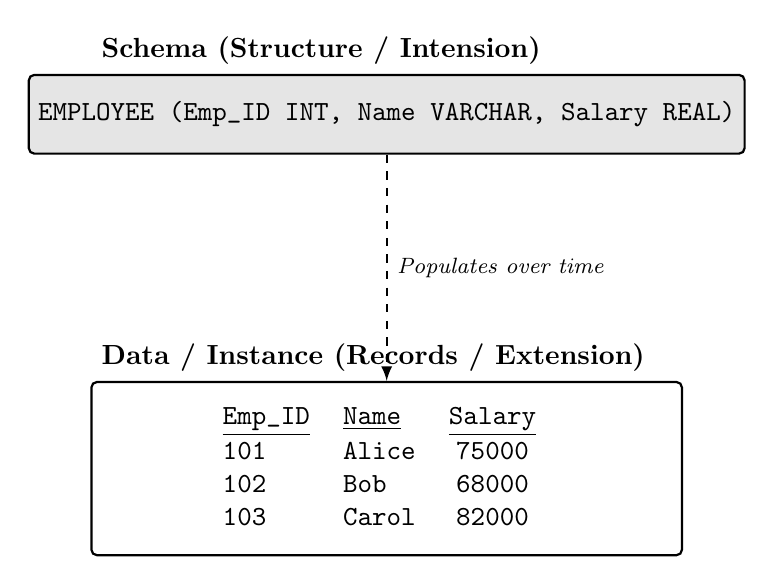
\begin{tikzpicture}[
    thick,
    box/.style={draw, rectangle, minimum width=7.5cm, align=center, rounded corners=2pt}
]
    % Schema Node
    \node[box, fill=black!10, minimum height=1cm, font=\ttfamily] (schema) at (0, 2) {EMPLOYEE (Emp\_ID INT, Name VARCHAR, Salary REAL)};
    \node[font=\bfseries, anchor=south west] at (-3.75, 2.5) {Schema (Structure / Intension)};

    % Data Node
    \node[box, minimum height=2.2cm, font=\ttfamily] (data) at (0, -2.5) {
        \begin{tabular}{llc}
        \underline{Emp\_ID} & \underline{Name} & \underline{Salary} \\
        101 & Alice & 75000 \\
        102 & Bob & 68000 \\
        103 & Carol & 82000 \\
        \end{tabular}
    };
    \node[font=\bfseries, anchor=south west] at (-3.75, -1.4) {Data / Instance (Records / Extension)};

    % Arrow
    \draw[->, >=latex, dashed, thick] (schema) -- (data) node[midway, right, font=\footnotesize\itshape] {Populates over time};
\end{tikzpicture}
\end{center}
\vspace{1em}

\begin{center}
\renewcommand{\arraystretch}{1.4}
\begin{tabular}{@{} >{\bfseries}l l l @{}}
\toprule
Feature & Database Schema & Database Data (Instance) \\
\midrule
\textbf{Definition} & The logical structure and rules of the database. & The actual content stored within the structure. \\
\textbf{Frequency of Change} & Rarely changes (static). & Changes constantly (dynamic). \\
\textbf{Metadata} & Stored in the database catalog (Data Dictionary). & Stored in the data files on the disk. \\
\textbf{Terminology} & Intension. & Extension. \\
\bottomrule
\end{tabular}
\end{center}

\vspace{1em}
\hrule
\vspace{1em}

\subsection*{2. DDL versus DML}

To interact with both the schema and the data, a DBMS provides specific categories of SQL languages: \textbf{Data Definition Language (DDL)} and \textbf{Data Manipulation Language (DML)}.

\begin{itemize}
    \item \textbf{DDL (Data Definition Language):} Used by database designers and administrators to specify, modify, or drop the \textbf{Database Schema}. Execution of DDL statements directly affects the Data Dictionary and is typically auto-committed (cannot be rolled back in standard relational systems).
    \begin{itemize}
        \item \textit{Common Commands:} \texttt{CREATE}, \texttt{ALTER}, \texttt{DROP}, \texttt{TRUNCATE}.
    \end{itemize}
    
    \item \textbf{DML (Data Manipulation Language):} Used by users and applications to retrieve, insert, delete, and modify the actual \textbf{Data (Instance)} stored within the tables. DML commands form the basis of transactional processing.
    \begin{itemize}
        \item \textit{Common Commands:} \texttt{SELECT}, \texttt{INSERT}, \texttt{UPDATE}, \texttt{DELETE}.
    \end{itemize}
\end{itemize}

\subsubsection*{Example Code Demonstration}
\begin{lstlisting}[language=SQL]
-- === DDL: Defining the Schema ===
CREATE TABLE Employee (
    Emp_ID INT PRIMARY KEY,
    Name VARCHAR(50),
    Salary DECIMAL(10,2)
);

-- === DML: Manipulating the Data / Instance ===
INSERT INTO Employee (Emp_ID, Name, Salary) VALUES (101, 'Alice', 75000);
UPDATE Employee SET Salary = 80000 WHERE Emp_ID = 101;
SELECT * FROM Employee;
\end{lstlisting}

\begin{center}
\renewcommand{\arraystretch}{1.4}
\begin{tabularx}{\textwidth}{@{} >{\bfseries}l X X @{}}
\toprule
Feature & DDL (Data Definition Language) & DML (Data Manipulation Language) \\
\midrule
\textbf{Target} & Operates on the \textbf{Schema} (metadata). & Operates on the \textbf{Data} (instances/records). \\
\textbf{Primary Users} & Database Administrators (DBA), Database Designers. & End Users, Application Programs. \\
\textbf{Transaction Control} & Usually auto-committed (cannot be rolled back). & Controlled by transaction blocks (can be rolled back). \\
\textbf{Effect} & Alters the structure (e.g., adding a column). & Alters the values (e.g., changing a salary). \\
\bottomrule
\end{tabularx}
\end{center}

\end{tcolorbox}

%% Q4
\item Explain the data dictionary schema for DBMS. List the advantages and disadvantages for storing a relational database as follows:
\begin{enumerate}
  \item Store each relation in one file.
  \item Store multiple relations in one file.
\end{enumerate}
\mk{10} \yr{CSE 303 | L-3/T-1 | 2010--11}

\begin{tcolorbox}[enhanced,breakable,ansbox,colback=cA!4,colframe=cA,boxrule=0.8pt,arc=5pt,title={\textbf{Answer}},fonttitle=\bfseries\color{white},colbacktitle=cA]

\subsection*{1. Data Dictionary Schema for DBMS}

\textbf{Definition:} The data dictionary (also known as the system catalog) is an internal database maintained by the DBMS to store \textbf{metadata}—that is, "data about the data." It acts as a comprehensive directory detailing the logical and physical structure of the entire database system. 

\textbf{Working Principle:} The DBMS itself accesses the data dictionary constantly. Before executing any query (DML or DDL), the Query Processor consults the data dictionary to verify that relations exist, attributes match, users have appropriate permissions, and to identify available indices for query optimization.

\textbf{Contents of a Data Dictionary:}
To manage this metadata, the DBMS stores the data dictionary as a set of relational tables. The schema of these system tables typically includes:
\begin{itemize}
    \item \textbf{Relation Information:} Names of all tables, views, their creators, and physical storage paths.
    \item \textbf{Attribute Information:} Names of attributes for each table, their data types, lengths, and constraints (e.g., NOT NULL).
    \item \textbf{Index Information:} Index names, the attributes they index, and the type of index (e.g., B+ tree, Hash).
    \item \textbf{Integrity Constraints:} Primary keys, foreign key references, and check constraints.
    \item \textbf{User and Authorization Data:} Usernames, passwords, and access privileges (Grants).
    \item \textbf{Statistical Data:} Number of tuples in a relation, distribution of values, used heavily by the Query Optimizer.
\end{itemize}

\subsubsection*{Visual Representation of a Simplified Data Dictionary Schema}

\vspace{1em}
\begin{center}
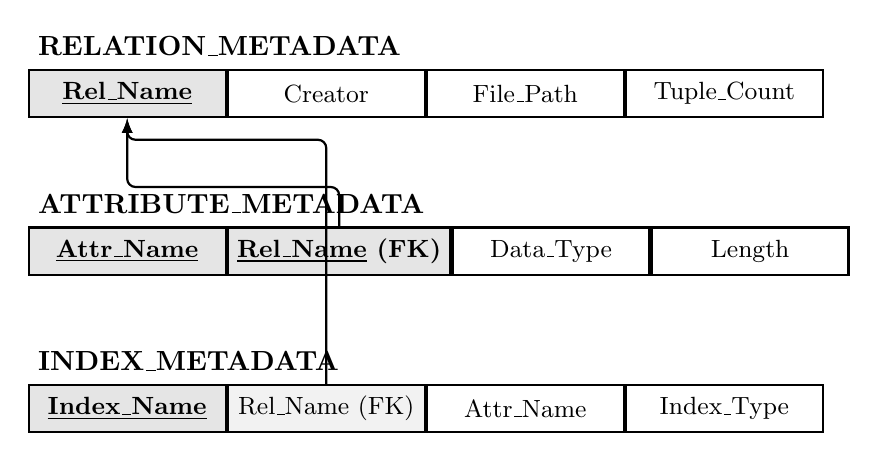
\begin{tikzpicture}[
    thick,x=1.3cm,
    tablebox/.style={draw, rectangle, minimum width=3cm, minimum height=0.6cm, align=center, fill=white, font=\small},
    attrbox/.style={draw, rectangle, minimum width=2.5cm, minimum height=0.6cm, align=center, fill=white, font=\small},
    pkbox/.style={draw, rectangle, minimum width=2.5cm, minimum height=0.6cm, align=center, fill=black!10, font=\small\bfseries},
    arrow/.style={->, >=latex, thick, rounded corners=3pt}
]

    % --- RELATION_METADATA Table ---
    \node[anchor=west, font=\bfseries] at (0, 3.6) {RELATION\_METADATA};
    \node[pkbox, anchor=west] (r1) at (0, 3) {\underline{Rel\_Name}};
    \node[attrbox, anchor=west] (r2) at (r1.east) {Creator};
    \node[attrbox, anchor=west] (r3) at (r2.east) {File\_Path};
    \node[attrbox, anchor=west] (r4) at (r3.east) {Tuple\_Count};

    % --- ATTRIBUTE_METADATA Table ---
    \node[anchor=west, font=\bfseries] at (0, 1.6) {ATTRIBUTE\_METADATA};
    \node[pkbox, anchor=west] (a1) at (0, 1) {\underline{Attr\_Name}};
    \node[pkbox, anchor=west] (a2) at (a1.east) {\underline{Rel\_Name} (FK)};
    \node[attrbox, anchor=west] (a3) at (a2.east) {Data\_Type};
    \node[attrbox, anchor=west] (a4) at (a3.east) {Length};

    % --- INDEX_METADATA Table ---
    \node[anchor=west, font=\bfseries] at (0, -0.4) {INDEX\_METADATA};
    \node[pkbox, anchor=west] (i1) at (0, -1) {\underline{Index\_Name}};
    \node[attrbox, anchor=west, fill=black!5] (i2) at (i1.east) {Rel\_Name (FK)};
    \node[attrbox, anchor=west] (i3) at (i2.east) {Attr\_Name};
    \node[attrbox, anchor=west] (i4) at (i3.east) {Index\_Type};

    % Foreign Key Relationships
    \draw[arrow] (a2.north) -- +(0, 0.5) -| (r1.south);
    \draw[arrow] (i2.north) -- +(0, 3.1) -| (r1.south);

\end{tikzpicture}
\end{center}
\vspace{1em}

\hrule
\vspace{1em}

\subsection*{2. Storing the Relational Database: File Strategies}

A DBMS needs a mapping between logical relations (tables) and physical operating system files. Two primary strategies exist, each with specific trade-offs.

\subsubsection*{Strategy 1: Store each relation in one separate file}
In this approach, every table in the database maps directly to its own isolated file on the disk (e.g., \texttt{Employee} maps to \texttt{employee.dat}, \texttt{Department} to \texttt{department.dat}).
\begin{center}
\begin{tabularx}{\textwidth}{@{} >{\bfseries}l X @{}}
\toprule
\multicolumn{2}{c}{\textbf{Each Relation in One File}} \\
\midrule
Advantages & 
\vspace{-1.2em}
\begin{itemize}
    \item \textbf{Simplicity:} The mapping between the database conceptual schema and physical files is extremely straightforward.
    \item \textbf{OS-Level Security:} The DBMS can leverage underlying Operating System file-level permissions to restrict access to specific tables.
    \item \textbf{Easy Maintenance:} Backing up, copying, or moving individual tables is very simple (just copy the specific file).
    \item \textbf{No Mixed-Record Overhead:} Because a file contains only one type of record (all the same length or structure), calculating record offsets and managing free space is mathematically simpler.
\end{itemize} \\
\midrule
Disadvantages & 
\vspace{-1.2em}
\begin{itemize}
    \item \textbf{OS Bottlenecks:} If a database contains thousands of tables, it results in thousands of files. Operating systems impose hard limits on the maximum number of simultaneously open file descriptors.
    \item \textbf{Join Performance Penalty:} Executing a \texttt{JOIN} operation between two relations requires the OS to open, read, and buffer multiple separate files concurrently, increasing disk I/O seek times and overhead.
    \item \textbf{Internal Fragmentation:} Small tables might waste disk space because the minimum allocation unit is a full OS disk block.
\end{itemize} \\
\bottomrule
\end{tabularx}
\end{center}
\vspace{1em}

\subsubsection*{Strategy 2: Store multiple relations in one file (Clustering)}
In this approach, the DBMS consolidates multiple relations—especially those that are frequently accessed together—into a single large, contiguous physical file (often referred to as a multitable clustering file organization).

\renewcommand{\arraystretch}{1.4}
\begin{tabularx}{\textwidth}{@{} >{\bfseries}l X @{}}
\toprule
\multicolumn{2}{c}{\textbf{Multiple Relations in One File}} \\
\midrule
Advantages & 
\vspace{-1.2em}
\begin{itemize}
    \item \textbf{Optimized Joins (Clustering):} Related records from different tables can be stored physically adjacent on the same disk block. For example, a \texttt{Department} record and all its associated \texttt{Employee} records can be read in a single disk I/O fetch, dramatically speeding up \texttt{JOIN} queries.
    \item \textbf{Overcoming OS Limits:} The DBMS uses very few OS files (sometimes just one massive file), completely avoiding OS limitations on the number of open file descriptors.
    \item \textbf{Space Efficiency:} Better packing of blocks reduces internal fragmentation, as small tables share blocks with other tables.
\end{itemize} \\
\midrule
Disadvantages & 
\vspace{-1.2em}
\begin{itemize}
    \item \textbf{High Complexity:} The DBMS must build and maintain its own internal file system and buffer manager logic to track where different table records reside within the single file.
    \item \textbf{Complex Space Reclamation:} When records of varying sizes from different tables are deleted, reclaiming the fragmented free space within the file is algorithmically difficult.
    \item \textbf{Sequential Scan Penalty:} Performing a sequential scan on a single table (\texttt{SELECT * FROM Employee}) becomes much slower. The DBMS must read the entire massive file and explicitly filter out the intermingled records belonging to other tables.
\end{itemize} \\
\bottomrule
\end{tabularx}

\end{tcolorbox}

\end{enumerate}

%%──────────────────────────────────────────────────────────────────────
\subtopic{cA}{Relational Model}
\label{sub:s1-relational}

\begin{enumerate}

%% Q1
\item Define super key, candidate key, and primary key with examples.
\mk{9} \yr{CSE 215 | L-2/T-1 | 2024--25}

\begin{tcolorbox}[enhanced,breakable,ansbox,colback=cA!4,colframe=cA,boxrule=0.8pt,arc=5pt,title={\textbf{Answer}},fonttitle=\bfseries\color{white},colbacktitle=cA]

\subsection*{1. Introduction and Running Example}
In the relational data model, keys are fundamental constraints used to uniquely identify tuples (rows) within a relation (table) and to establish relationships between different relations. 

To illustrate these concepts, consider the following relation schema for a university system:
\begin{center}
    \textbf{STUDENT( \underline{Roll\_No}, Reg\_No, Email, Name, Age, Branch )}
\end{center}
\textit{Assumption:} \texttt{Roll\_No}, \texttt{Reg\_No} (Registration Number), and \texttt{Email} are strictly unique for every student. Two students may share the same \texttt{Name}, \texttt{Age}, or \texttt{Branch}.

\subsection*{2. Definitions and Mathematical Properties}

\subsubsection*{A. Super Key}
\begin{itemize}
    \item \textbf{Definition:} A Super Key is a set of one or more attributes whose combined values uniquely identify a tuple within a relation.
    \item \textbf{Mathematical Property (Uniqueness):} Let $R$ be a relation schema. A subset of attributes $K \subseteq R$ is a super key if the functional dependency $K \rightarrow R$ holds.
    \item \textbf{Examples:} 
    \begin{itemize}
        \item $\{\text{Roll\_No}\}$
        \item $\{\text{Reg\_No}, \text{Name}\}$
        \item $\{\text{Email}, \text{Age}, \text{Branch}\}$
        \item $\{\text{Roll\_No}, \text{Reg\_No}, \text{Email}, \text{Name}, \text{Age}, \text{Branch}\}$ (The trivial super key comprising all attributes).
    \end{itemize}
    \item \textbf{Note:} Adding any arbitrary attribute to a super key results in another valid super key.
\end{itemize}

\subsubsection*{B. Candidate Key}
\begin{itemize}
    \item \textbf{Definition:} A Candidate Key is a \textbf{minimal} super key. It is a super key such that no proper subset of its attributes also constitutes a super key.
    \item \textbf{Mathematical Property (Minimality):} $K$ is a candidate key if $K$ is a super key, and for any proper subset $K' \subset K$, $K'$ is \textit{not} a super key.
    \item \textbf{Examples:} 
    \begin{itemize}
        \item $\{\text{Roll\_No}\}$ (Minimal, removing it leaves the empty set).
        \item $\{\text{Reg\_No}\}$ 
        \item $\{\text{Email}\}$
    \end{itemize}
    \item \textit{Why is $\{\text{Reg\_No}, \text{Name}\}$ NOT a Candidate Key?} Because its proper subset $\{\text{Reg\_No}\}$ is already a super key. Thus, it violates the minimality condition.
\end{itemize}

\subsubsection*{C. Primary Key}
\begin{itemize}
    \item \textbf{Definition:} The Primary Key is the specific candidate key selected by the database designer to principally identify tuples in the relation.
    \item \textbf{Properties:} 
    \begin{itemize}
        \item A relation can have \textbf{only one} primary key.
        \item Its attributes cannot contain \texttt{NULL} values (Entity Integrity Constraint).
        \item Its values should ideally remain immutable (unchanging) over time.
    \end{itemize}
    \item \textbf{Example:} From the candidate keys $\{\text{Roll\_No}\}$, $\{\text{Reg\_No}\}$, and $\{\text{Email}\}$, the designer selects \textbf{$\{\text{Roll\_No}\}$} as the Primary Key. 
    \item \textbf{Note:} The unselected candidate keys ($\{\text{Reg\_No}\}$ and $\{\text{Email}\}$) are then referred to as \textbf{Alternate Keys}.
\end{itemize}

\subsection*{3. Visualizing the Relationship}

The relationship between these keys can be accurately represented using set theory. All candidate keys are super keys, and the primary key is exactly one of the candidate keys.

\vspace{1.5em}
\begin{center}
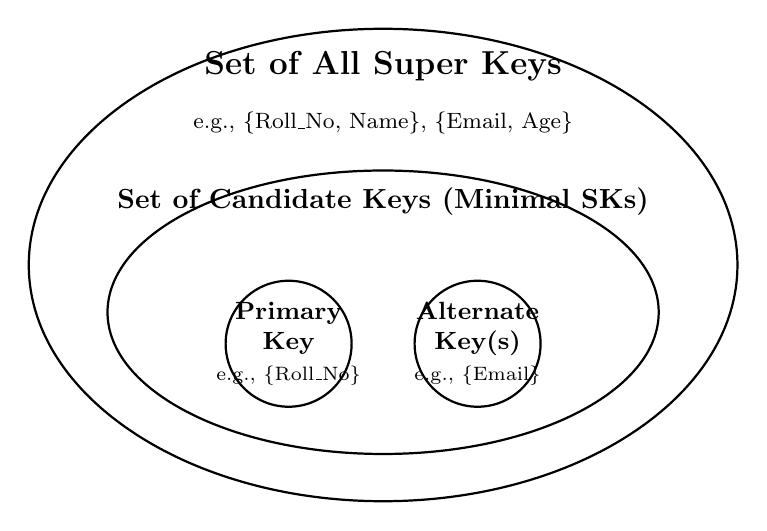
\begin{tikzpicture}[thick]
    % Outer set: Super Keys
    \draw (0,0) ellipse (4.5cm and 3cm);
    \node[anchor=south, font=\bfseries\large] at (0, 2.2) {Set of All Super Keys};
    
    % Example of non-minimal super key
    \node[font=\footnotesize] at (0, 1.8) {e.g., \{Roll\_No, Name\}, \{Email, Age\}};
    
    % Inner set: Candidate Keys
    \draw (0,-0.6) ellipse (3.5cm and 1.8cm);
    \node[anchor=south, font=\bfseries] at (0, 0.5) {Set of Candidate Keys (Minimal SKs)};
    
    % Primary Key subset
    \draw (-1.2, -1) circle (0.8cm);
    \node[align=center, font=\small\bfseries] at (-1.2, -1) {Primary\\Key\\ \normalfont \scriptsize e.g., \{Roll\_No\}};
    
    % Alternate Key subset
    \draw (1.2, -1) circle (0.8cm);
    \node[align=center, font=\small\bfseries] at (1.2, -1) {Alternate\\Key(s)\\ \normalfont \scriptsize e.g., \{Email\}};
    
\end{tikzpicture}
\end{center}
\vspace{1em}

\subsection*{4. Comparison Summary}

\begin{center}
\renewcommand{\arraystretch}{1.4}
\begin{tabularx}{\textwidth}{@{} >{\bfseries}l X X X @{}}
\toprule
Feature & Super Key & Candidate Key & Primary Key \\
\midrule
\textbf{Definition} & Uniquely identifies a tuple. & A minimal super key. & The chosen candidate key. \\
\textbf{Quantity} & Many per relation. & One or more per relation. & Exactly one per relation. \\
\textbf{Minimality} & Not required. & Strictly required. & Strictly required. \\
\textbf{Null Values} & May contain NULLs (if other attributes ensure uniqueness). & Cannot contain NULLs (in practice). & Strictly prohibits NULLs. \\
\textbf{Subset Relation} & The superset of all keys. & A subset of Super Keys. & A subset of Candidate Keys. \\
\bottomrule
\end{tabularx}
\end{center}


\end{tcolorbox}

\item Suppose we have two relations $A$ and $B$ with the same set of attributes. Relation $A$ has $n_a$ tuples and relation $B$ has $n_b$ tuples. For each of the following relational algebra expressions, give the minimum and maximum number of tuples that can appear in the result. Assume that the produced results are bags, not sets.
\begin{enumerate}
  \item $A \cap B$
  \item $\sigma_c(A) - B$
  \item $A \cup B$
  \item $A \bowtie_L B$, where $\bowtie_L$ is the left outer join
\end{enumerate}
\mk{8} \yr{CSE 215 | L-2/T-2 | 2020--21}

\begin{tcolorbox}[enhanced,breakable,ansbox,colback=cA!4,colframe=cA,boxrule=0.8pt,arc=5pt,title={\textbf{Answer}},fonttitle=\bfseries\color{white},colbacktitle=cA]

\subsection*{Bag Semantics Overview}
In relational algebra, standard operations often assume \textbf{set semantics} (where duplicates are eliminated). However, real-world Database Management Systems (DBMS) typically use \textbf{bag (multiset) semantics}, where duplicates are retained unless explicitly removed. 

Let a tuple $t$ appear $x$ times in relation $A$ (where $\sum x = n_a$) and $y$ times in relation $B$ (where $\sum y = n_b$). The output cardinality depends on how the specific bag operation computes the new frequency for each tuple.

---

\subsubsection*{1. Intersection ($A \cap B$)}
\begin{itemize}
    \item \textbf{Working Principle:} Under bag semantics, the intersection retains a tuple $t$ exactly $\min(x, y)$ times.
    \item \textbf{Minimum Tuples:} $\mathbf{0}$. This occurs when relations $A$ and $B$ are completely disjoint (they share no tuples in common).
    \item \textbf{Maximum Tuples:} $\mathbf{\min(n_a, n_b)}$. This occurs when all tuples of the smaller relation are entirely contained within the larger relation.
\end{itemize}

\subsubsection*{2. Selection and Difference ($\sigma_c(A) - B$)}
\begin{itemize}
    \item \textbf{Working Principle:} First, the selection $\sigma_c(A)$ filters $A$. The number of tuples generated by $\sigma_c(A)$ can range from $0$ to $n_a$. Next, the bag difference $X - B$ computes the frequency of tuple $t$ as $\max(0, count(t \in X) - y)$.
    \item \textbf{Minimum Tuples:} $\mathbf{0}$. This occurs if the selection condition $c$ matches no tuples in $A$ (yielding 0 tuples), OR if all tuples generated by $\sigma_c(A)$ also exist in $B$ in equal or greater quantities, causing them to be entirely subtracted out.
    \item \textbf{Maximum Tuples:} $\mathbf{n_a}$. This occurs if the selection condition $c$ is true for all tuples in $A$ (yielding $n_a$ tuples), AND relations $A$ and $B$ are completely disjoint, meaning no tuples are subtracted by $B$.
\end{itemize}

\subsubsection*{3. Union ($A \cup B$)}
\begin{itemize}
    \item \textbf{Working Principle:} Under bag semantics, union does \textbf{not} eliminate duplicates (equivalent to \texttt{UNION ALL} in SQL). The frequency of a tuple $t$ in the result is simply $x + y$. 
    \item \textbf{Minimum Tuples:} $\mathbf{n_a + n_b}$.
    \item \textbf{Maximum Tuples:} $\mathbf{n_a + n_b}$.
    \item \textbf{Note:} Unlike set union (which can range from $\max(n_a, n_b)$ to $n_a + n_b$), bag union always yields exactly the sum of the cardinalities of the two input relations.
\end{itemize}

\subsubsection*{4. Left Outer Join ($A \bowtie_L B$)}
\begin{itemize}
    \item \textbf{Working Principle:} Because $A$ and $B$ have the \textit{same set of attributes}, the join condition evaluates all attributes for equality (Natural Left Outer Join). 
    \begin{itemize}
        \item If a tuple in $A$ finds matching tuples in $B$ ($y > 0$), it produces $x \times y$ copies.
        \item If it finds no match ($y = 0$), the Left Outer Join ensures the tuple from $A$ is preserved exactly $x$ times, padded with NULLs (though here, all attributes overlap).
    \end{itemize}
    Mathematically, the total tuples are $\sum (x \cdot \max(y, 1))$.
    \item \textbf{Minimum Tuples:} $\mathbf{n_a}$. This occurs either when $A$ and $B$ are completely disjoint (every tuple in $A$ gets preserved exactly once with no matches), or when every tuple in $A$ matches exactly one tuple in $B$.
    \item \textbf{Maximum Tuples:} $\mathbf{\max(n_a, n_a \times n_b)}$. If $n_b > 0$, the maximum is $n_a \times n_b$. This explosion occurs when every tuple in $A$ is identical, and every tuple in $B$ is also identical to the tuples in $A$, resulting in a full Cartesian product. If $B$ is empty ($n_b = 0$), the maximum is simply $n_a$.
\end{itemize}

---

\subsection*{Summary Table}

\begin{center}
\renewcommand{\arraystretch}{1.5}
\begin{tabularx}{0.9\textwidth}{@{} >{\bfseries}l X X @{}}
\toprule
Relational Algebra Expression & Minimum Tuples & Maximum Tuples \\
\midrule
$A \cap B$ & $0$ & $\min(n_a, n_b)$ \\
$\sigma_c(A) - B$ & $0$ & $n_a$ \\
$A \cup B$ & $n_a + n_b$ & $n_a + n_b$ \\
$A \bowtie_L B$ & $n_a$ & $\max(n_a, n_a \cdot n_b)$ \\
\bottomrule
\end{tabularx}
\end{center}


\end{tcolorbox}


\item Should a primary key have any semantic meaning? Explain your answer.
\mk{6} \yr{CSE 303 | L-3/T-1 | 2014--15}

\begin{tcolorbox}[enhanced,breakable,ansbox,colback=cA!4,colframe=cA,boxrule=0.8pt,arc=5pt,title={\textbf{Answer}},fonttitle=\bfseries\color{white},colbacktitle=cA]

\subsection*{1. Direct Answer}
Ideally, \textbf{no}. A primary key should generally \textbf{not} have any semantic (real-world business) meaning. 

In database design, keys are divided into two categories based on meaning:
\begin{itemize}
    \item \textbf{Natural Key (Semantic):} An attribute that has a logical relationship to the business data (e.g., Social Security Number, Email Address, Vehicle Identification Number).
    \item \textbf{Surrogate Key (Meaningless):} An artificially generated attribute with no real-world meaning, created solely to identify a tuple uniquely (e.g., an Auto-Incrementing Integer, UUID/GUID).
\end{itemize}

Best practices in modern database design strongly favor the use of \textbf{Surrogate Keys} for primary keys, while applying \texttt{UNIQUE} constraints to Natural Keys.

\subsection*{2. Why Semantic Primary Keys are Problematic}

Using a semantic attribute as a primary key introduces several risks to the stability and performance of a relational database:

\begin{enumerate}
    \item \textbf{Mutability (Data Changes):} Semantic data is tied to business rules and human behavior, meaning it is subject to change. For example, if an \texttt{Email} is used as a primary key and the user changes their email address, the database must perform a cascading update to every foreign key in every related table (e.g., Orders, Logs, Profiles). A surrogate key, being meaningless, never needs to change.
    \item \textbf{Format and Business Rule Changes:} Business rules evolve. A 9-digit alphanumeric product code might be expanded to 12 digits. If this code is a primary key, altering the data type or length across millions of foreign key references is an expensive and risky operation.
    \item \textbf{Reusability:} Some semantic identifiers get recycled over time (e.g., phone numbers or invoice numbers). Reusing a primary key can lead to catastrophic data integrity issues where old, unrelated records accidentally link to new entities.
    \item \textbf{Privacy and Security:} Primary keys are frequently exposed in URLs, log files, and API endpoints. Using sensitive semantic data (like an SSN or phone number) as a primary key leaks personally identifiable information (PII).
    \item \textbf{Performance (Storage and Indexing):} Semantic keys are often long strings (like \texttt{VARCHAR(255)} for an email). String comparisons are significantly slower than integer comparisons. Furthermore, B+ Tree indexes built on large strings consume more memory and disk space. A surrogate key, typically a 4-byte or 8-byte integer, is highly optimized for fast \texttt{JOIN} operations.
\end{enumerate}

\subsection*{3. Visualizing the Recommended Approach}

Instead of forcing a semantic attribute to act as the primary key, database designers implement a surrogate primary key and designate the semantic attributes as \textbf{Alternate Keys} (using the \texttt{UNIQUE} constraint).

\vspace{1.5em}
\begin{center}
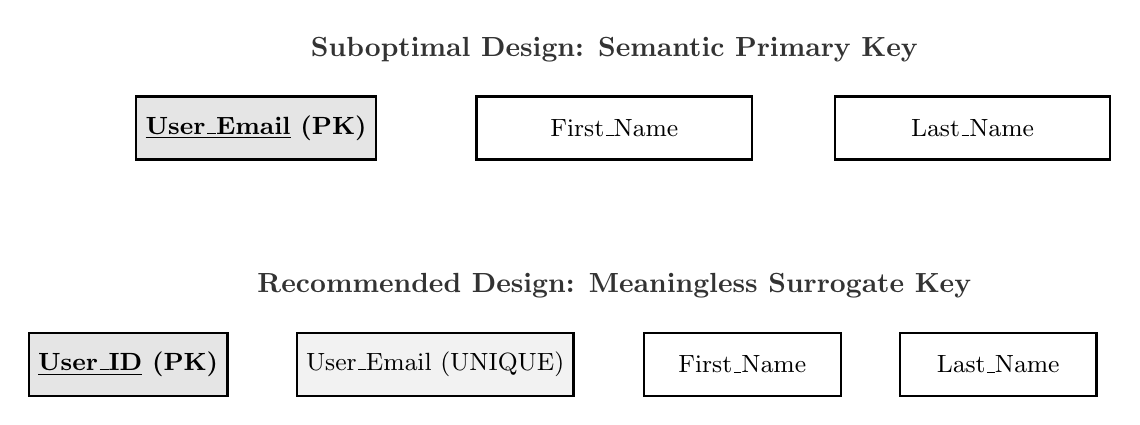
\begin{tikzpicture}[
    thick,x=1.3cm,
    pkbox/.style={draw, rectangle, minimum width=3cm, minimum height=0.8cm, align=center, fill=black!10, font=\small\bfseries},
    attrbox/.style={draw, rectangle, minimum width=3.5cm, minimum height=0.8cm, align=center, fill=white, font=\small}
]
    % Bad Design
    \node[font=\bfseries, text=black!80] at (0, 2) {Suboptimal Design: Semantic Primary Key};
    \node[pkbox] (n1) at (-3.5, 1) {\underline{User\_Email} (PK)};
    \node[attrbox] (n2) at (0, 1) {First\_Name};
    \node[attrbox] (n3) at (3.5, 1) {Last\_Name};
    
    % Good Design
    \node[font=\bfseries, text=black!80] at (0, -1) {Recommended Design: Meaningless Surrogate Key};
    \node[pkbox, minimum width=2.5cm] (s1) at (-4.75, -2) {\underline{User\_ID} (PK)};
    \node[attrbox, minimum width=3.5cm, fill=black!5] (s2) at (-1.75, -2) {User\_Email (UNIQUE)};
    \node[attrbox, minimum width=2.5cm] (s3) at (1.25, -2) {First\_Name};
    \node[attrbox, minimum width=2.5cm] (s4) at (3.75, -2) {Last\_Name};
    
\end{tikzpicture}
\end{center}
\vspace{1em}

\subsection*{4. Comparison: Natural (Semantic) vs. Surrogate (Meaningless) Keys}

\begin{center}
\renewcommand{\arraystretch}{1.4}
\begin{tabular}{@{} p{3.5cm} p{5.5cm} p{5.5cm} @{}}
\toprule
\textbf{Feature} & \textbf{Natural Key (Semantic)} & \textbf{Surrogate Key (Meaningless)} \\
\midrule
\textbf{Origin} & Exists in the real world (e.g., SSN). & System-generated (e.g., Auto-increment). \\
\textbf{Immutability} & Prone to change if business rules change. & 100\% Immutable. Never changes. \\
\textbf{Performance} & Often slow (e.g., long strings). & Very fast (e.g., 32/64-bit integers). \\
\textbf{Coupling} & Tightly couples DB structure to business rules. & Decouples structure from business logic. \\
\textbf{Use Case} & Enforce uniqueness (Alternate Key). & Primary Key / Foreign Key relationships. \\
\bottomrule
\end{tabular}
\end{center}

\vspace{1em}
\noindent\textbf{Notes:} While surrogate keys are generally preferred, there is one major exception: \textbf{Link Tables} (Junction Tables) used to resolve Many-to-Many relationships. In a link table (e.g., \texttt{Enrollment(Student\_ID, Course\_ID)}), the primary key should be the composite of the two foreign keys, which intrinsically carries semantic meaning regarding the relationship.

\end{tcolorbox}

\item Describe with an example, the object identity and reference types in SQL. How can you process queries using reference type?
\mk{10} \yr{CSE 303 | L-3/T-1 | 2010--11}

\begin{tcolorbox}[enhanced,breakable,ansbox,colback=cA!4,colframe=cA,boxrule=0.8pt,arc=5pt,title={\textbf{Answer}},fonttitle=\bfseries\color{white},colbacktitle=cA]

\subsection*{1. Object Identity in SQL}

In standard relational databases, tuples (rows) are identified purely by their values, specifically through a \textbf{Primary Key}. However, in \textbf{Object-Relational Database Management Systems (ORDBMS)} complying with the SQL:1999 standard and later, tuples can be treated as unique objects.

\begin{itemize}
    \item \textbf{Object Identity (OID):} When a row is inserted into a ``typed table'' (a table built upon a user-defined complex data type), the DBMS assigns it a unique, system-generated, and immutable Object Identifier (OID).
    \item \textbf{Properties of OID:} Unlike primary keys, an OID has no real-world semantic meaning, does not depend on the object's attribute values, and never changes even if all the data within the row is updated.
\end{itemize}

\subsection*{2. Reference Types (\texttt{REF})}

A \textbf{Reference Type} is a special data type in SQL that stores an OID. It acts essentially as a strongly-typed \textbf{pointer} to a specific object (row) in another typed table.
\begin{itemize}
    \item \textbf{Working Principle:} Instead of using standard Foreign Keys that store copies of Primary Key values (which requires traditional joins), a \texttt{REF} attribute directly points to the memory/disk location of the referenced object, enabling highly efficient object traversal.
    \item \textbf{Scoping:} A reference type is usually constrained using a \texttt{SCOPE} clause to ensure it only points to objects within a specific target table.
\end{itemize}

\subsection*{3. Example Scenario: DDL for Objects and References}

Consider a university system where an \texttt{Employee} works for a \texttt{Department}. First, we define the object types, and then we create the typed tables.

\begin{lstlisting}[language=SQL]
-- 1. Create the base User-Defined Types (UDT)
CREATE TYPE DepartmentType AS (
    Dept_No INT,
    Dept_Name VARCHAR(50)
);

CREATE TYPE EmployeeType AS (
    Emp_ID INT,
    Name VARCHAR(50),
    Works_For REF(DepartmentType) -- The Reference Type
);

-- 2. Create Typed Tables
CREATE TABLE Departments OF DepartmentType (
    REF IS Dept_OID SYSTEM GENERATED, -- Explicitly generating OIDs
    PRIMARY KEY (Dept_No)
);

CREATE TABLE Employees OF EmployeeType (
    PRIMARY KEY (Emp_ID),
    SCOPE FOR Works_For IS Departments -- Restricting pointer target
);
\end{lstlisting}

\subsection*{4. Visualizing Object References}

\vspace{1em}

\begin{center}
    % ------ Employees Table (Source) ------
    \begin{minipage}[t]{0.45\textwidth}
        \centering
        \textbf{Employees Table (Source)}\\[0.5em]
        \renewcommand{\arraystretch}{1.3} % Adds a little vertical padding
        \begin{tabular}{|c|c|c|}
            \hline
            \rowcolor{black!10} 
            \textbf{Emp\_ID} & \textbf{Name} & \textbf{Works\_For} \\
            \hline
            101 & Alice & \cellcolor{blue!5}\textit{0x9A4F...} \\
            \hline
        \end{tabular}
    \end{minipage}\hfill
    % ------ Departments Table (Target) ------
    \begin{minipage}[t]{0.5\textwidth}
        \centering
        \textbf{Departments Table (Target)}\\[0.5em]
        \renewcommand{\arraystretch}{1.3}
        \begin{tabular}{|c|c|c|}
            \hline
            \rowcolor{black!10} 
            \textbf{OID (System)} & \textbf{Dept\_No} & \textbf{Dept\_Name} \\
            \hline
            \cellcolor{blue!5}\textit{0x9A4F...} & 10 & Research \\
            \hline
        \end{tabular}
    \end{minipage}

    \vspace{1.5em}
    
    % ------ Reference Indicator ------
    \textbf{0x9A4F...} $\xrightarrow{\hspace{1cm} \text{Dereference (Pointer Traversal)} \hspace{1cm}}$ \textbf{0x9A4F...}
    
\end{center}

\vspace{1em}

\subsection*{5. Query Processing Using Reference Types}

To process queries involving reference types, standard \texttt{JOIN} operations can be entirely bypassed. Instead, object-relational SQL introduces \textbf{Path Expressions} and \textbf{Dereferencing}.

\subsubsection*{A. Dereferencing Operator (\texttt{->})}
The \texttt{->} operator takes a \texttt{REF} value and retrieves the object it points to, allowing direct access to the target object's attributes.

\begin{lstlisting}[language=SQL]
-- Retrieve employee names and the name of the department they work for.
-- Notice the absence of a JOIN clause.
SELECT e.Name, 
       e.Works_For->Dept_Name AS Department_Name
FROM Employees e;
\end{lstlisting}

\subsubsection*{B. The \texttt{DEREF()} Function}
If the goal is to return the entire referenced object (tuple) rather than just a specific attribute, the \texttt{DEREF()} function is utilized.

\begin{lstlisting}[language=SQL]
-- Retrieve the full Department object for the employee named Alice
SELECT DEREF(e.Works_For) AS Dept_Object
FROM Employees e
WHERE e.Name = 'Alice';
\end{lstlisting}

\subsection*{6. Advantages of Object References}
\begin{itemize}
    \item \textbf{Performance (Implicit Joins):} Traversing pointers is computationally faster than performing hash-joins or sort-merge joins on standard foreign keys.
    \item \textbf{Simpler Query Syntax:} Complex, multi-table relationships can be queried cleanly using cascading path expressions (e.g., \texttt{a->b->c}) without cluttering the \texttt{FROM} clause.
    \item \textbf{Polymorphism:} References can be designed to point to an object of a super-type or any of its sub-types, enabling polymorphic queries.
\end{itemize}

\end{tcolorbox}

\end{enumerate}

%% ── S2: Database Design ───────────────────────────────────────────────
\section{S2 --- Database Design}
\label{sec:S2}
\markboth{S2 --- Database Design}{}

%%──────────────────────────────────────────────────────────────────────
\subtopic{cA}{Entity-Relationship (ER) Model}
\label{sub:s2-er}

\begin{enumerate}


\item Differentiate between strong entity and weak entity by showing appropriate examples. How do you design them in a relational schema?
\mk{10} \yr{CSE 215 | L-2/T-2 | 2018--19}

\begin{tcolorbox}[enhanced,breakable,ansbox,colback=cA!4,colframe=cA,boxrule=0.8pt,arc=5pt,title={\textbf{Answer}},fonttitle=\bfseries\color{white},colbacktitle=cA]

\subsection*{1. Distinction Between Strong and Weak Entities}

In Entity-Relationship (ER) modeling, entities are categorized based on their ability to be uniquely identified strictly by their own attributes.

\begin{itemize}
    \item \textbf{Strong Entity:} An entity type that possesses a \textbf{Primary Key}. It has an independent existence in the database and does not rely on any other entity for its identification.
    \item \textbf{Weak Entity:} An entity type that does \textbf{not} have sufficient attributes to form a primary key. It depends on a strong entity (called the \textbf{Identifying Owner}) for its existence and identification. It uses a \textbf{Partial Key} (or Discriminator) combined with the primary key of its owner to uniquely identify its instances.
\end{itemize}

\subsubsection*{Comparison Table}
\begin{center}
\renewcommand{\arraystretch}{1.4}
\begin{tabularx}{\textwidth}{@{} >{\bfseries}l X X @{}}
\toprule
Feature & Strong Entity & Weak Entity \\
\midrule
\textbf{Primary Key} & Has its own primary key. & Does not have a primary key; has a partial key. \\
\textbf{Existence} & Independent existence. & Existence depends on the identifying strong entity. \\
\textbf{Relationship} & Associated via standard relationships. & Associated via an \textbf{identifying relationship}. \\
\textbf{Participation} & Can have total or partial participation. & \textbf{Always} has total participation in the identifying relationship. \\
\textbf{ER Diagram} & Represented by a single rectangle. & Represented by a double rectangle. \\
\bottomrule
\end{tabularx}
\end{center}

\subsection*{2. Example and ER Diagram Representation}

\textbf{Example Scenario:} Consider a company database storing information about \texttt{EMPLOYEE}s and their \texttt{DEPENDENT}s (spouses, children). 
\begin{itemize}
    \item \texttt{EMPLOYEE} is a \textbf{Strong Entity} uniquely identified by \texttt{Emp\_ID}.
    \item \texttt{DEPENDENT} is a \textbf{Weak Entity}. A dependent's name (\texttt{Dep\_Name}) only identifies them uniquely \textit{within} the context of a specific employee. It cannot uniquely identify a dependent across the entire company.
\end{itemize}

\vspace{1em}
\begin{center}
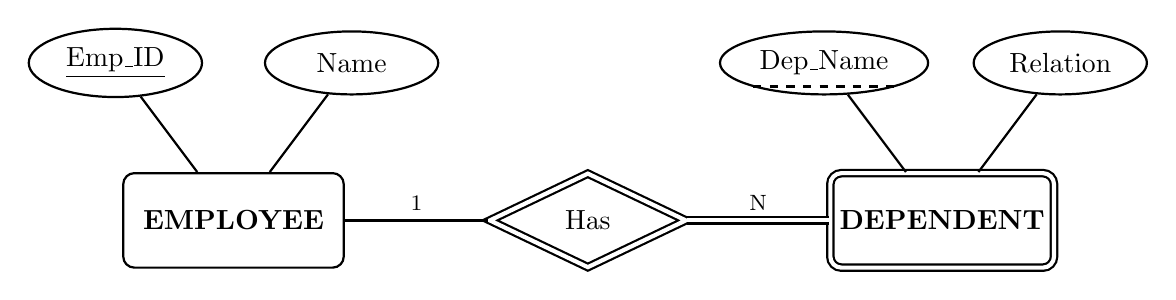
\begin{tikzpicture}[
    thick,
    entity/.style={draw, rectangle, rounded corners, minimum width=2.8cm, minimum height=1.2cm, align=center, fill=white},
    weakentity/.style={draw, double, double distance=1.5pt, rectangle, rounded corners, minimum width=2.8cm, minimum height=1.2cm, align=center, fill=white},
    relationship/.style={draw, diamond, aspect=1.5, minimum width=2.5cm, minimum height=1.2cm, align=center, fill=white},
    identrel/.style={draw, double, double distance=1.5pt, diamond, aspect=1.5, minimum width=2.5cm, minimum height=1.2cm, align=center, fill=white},
    attribute/.style={draw, ellipse, minimum width=2.2cm, minimum height=0.8cm, align=center, fill=white}
]
    % Entities and Relationships
    \node[entity] (emp) at (0,0) {\textbf{EMPLOYEE}};
    \node[identrel] (has) at (4.5,0) {Has};
    \node[weakentity] (dep) at (9,0) {\textbf{DEPENDENT}};

    % Employee Attributes
    \node[attribute] (empid) at (-1.5, 2) {\underline{Emp\_ID}};
    \node[attribute] (name) at (1.5, 2) {Name};

    % Dependent Attributes
    \node[attribute] (depname) at (7.5, 2) {Dep\_Name};
    % Manual dashed underline for partial key
    \draw[dashed, thick] (6.6, 1.7) -- (8.4, 1.7);
    \node[attribute] (relation) at (10.5, 2) {Relation};

    % Connections
    \draw (emp) -- (empid);
    \draw (emp) -- (name);
    
    \draw (dep) -- (depname);
    \draw (dep) -- (relation);

    % Participation lines (Single for Strong, Double for Weak)
    \draw (emp) -- (has) node[midway, above, font=\footnotesize] {1};
    \draw[double, double distance=1.5pt] (has) -- (dep) node[midway, above, font=\footnotesize] {N};

\end{tikzpicture}
\end{center}
\vspace{1em}

\subsection*{3. Design in a Relational Schema}

To convert a strong and weak entity relationship into a relational database schema, apply the following mapping rules:

\begin{enumerate}
    \item \textbf{Strong Entity Mapping:} Create a separate table for the strong entity. Its attributes become columns, and its key attribute becomes the \textbf{Primary Key (PK)}.
    \item \textbf{Weak Entity Mapping:} Create a separate table for the weak entity. Include all of its own attributes. Then, add the Primary Key of the identifying strong entity as a \textbf{Foreign Key (FK)}.
    \item \textbf{Weak Entity Primary Key:} The Primary Key of the weak entity table is a \textbf{Composite Key} formed by combining its Foreign Key and its Partial Key.
\end{enumerate}

\subsubsection*{Relational Schema Diagram}

\vspace{1em}
\begin{center}
    % Increase row height for a spacious, readable look
    \renewcommand{\arraystretch}{1.8} 
    % Sans-serif font often looks cleaner for database schemas
    \sffamily 

    % ------ EMPLOYEE Table ------
    \begin{tabular}{|>{\columncolor{black!10}\bfseries\centering\arraybackslash}m{2.8cm}|>{\centering\arraybackslash}m{2.8cm}|>{\centering\arraybackslash}m{2.8cm}|}
        \hline
        EMPLOYEE & \underline{\textbf{Emp\_ID}} & Name \\
        \hline
    \end{tabular}

    \vspace{1.5em}

    % ------ DEPENDENT Table ------
    \begin{tabular}{|>{\columncolor{black!10}\bfseries\centering\arraybackslash}m{2.8cm}|>{\centering\arraybackslash}m{2.8cm}|>{\centering\arraybackslash}m{2.8cm}|>{\centering\arraybackslash}m{2.8cm}|}
        \hline
        DEPENDENT & \underline{\textbf{Emp\_ID}} \newline \scriptsize(FK) & \underline{\textbf{Dep\_Name}} & Relation \\
        \hline
    \end{tabular}
    
\end{center}

\vspace{0.5em}

% ------ Notes and Relationships ------
\begin{flushleft}
    \footnotesize\textit{* \textbf{Note:} The primary key of DEPENDENT is composite: (\textbf{Emp\_ID}, \textbf{Dep\_Name}).}\\
    \footnotesize\textit{** \textbf{Foreign Key Mapping:} DEPENDENT.\textbf{Emp\_ID} $\rightarrow$ EMPLOYEE.\textbf{Emp\_ID}}
\end{flushleft}

\vspace{1em}

\end{tcolorbox}

\item Define weak entity set. Also give an example of a weak entity set.
\mk{5} \yr{CSE 215 | L-2/T-2 | 2017--18}

\begin{tcolorbox}[enhanced,breakable,ansbox,colback=cA!4,colframe=cA,boxrule=0.8pt,arc=5pt,title={\textbf{Answer}},fonttitle=\bfseries\color{white},colbacktitle=cA]

\subsection*{1. Definition}
A \textbf{weak entity set} is an entity type that does not contain sufficient attributes to uniquely identify its own entities (i.e., it lacks a primary key of its own). To be uniquely identified, a weak entity must be associated with another entity set, known as the \textbf{identifying entity set} (or strong entity set).

\subsection*{2. Key Characteristics}
\begin{itemize}
    \item \textbf{Existence Dependency:} A weak entity cannot exist in the database without its corresponding strong entity. If the strong entity is deleted, all its associated weak entities must also be deleted (cascade delete).
    \item \textbf{Identifying Relationship:} The relationship associating the weak entity set with the strong entity set is called the identifying relationship. In an Entity-Relationship (ER) diagram, it is denoted by a \textbf{double diamond}.
    \item \textbf{Total Participation:} The weak entity set always exhibits total participation (denoted by a \textbf{double line}) in the identifying relationship, meaning every weak entity must be related to an identifying entity.
    \item \textbf{Partial Key (Discriminator):} Instead of a primary key, a weak entity set has a \textbf{partial key} (or discriminator). This is an attribute (or set of attributes) that uniquely identifies weak entities related to the \textit{same} strong entity. It is denoted by a \textbf{dashed underline} in an ER diagram.
    \item \textbf{Primary Key Formation:} The actual primary key of a weak entity is a composite key formed by combining the primary key of the strong entity set with the weak entity set's partial key.
\end{itemize}

\subsection*{3. Example Scenario}
Consider a company database that stores information about employees and their dependents (e.g., spouses, children) for health insurance purposes. 
\begin{itemize}
    \item \textbf{Strong Entity Set:} \texttt{EMPLOYEE} (uniquely identified by \texttt{Emp\_ID}).
    \item \textbf{Weak Entity Set:} \texttt{DEPENDENT}. A dependent's name (\texttt{Dep\_Name}) is not globally unique across the whole company, but it is unique for a specific employee. 
    \item \textbf{Identifying Relationship:} \texttt{Policy\_Covers}.
\end{itemize}

In this context, a dependent only exists in the database if their associated employee exists. 

\subsection*{4. ER Diagram Representation}

\vspace{1.5em}
\begin{center}
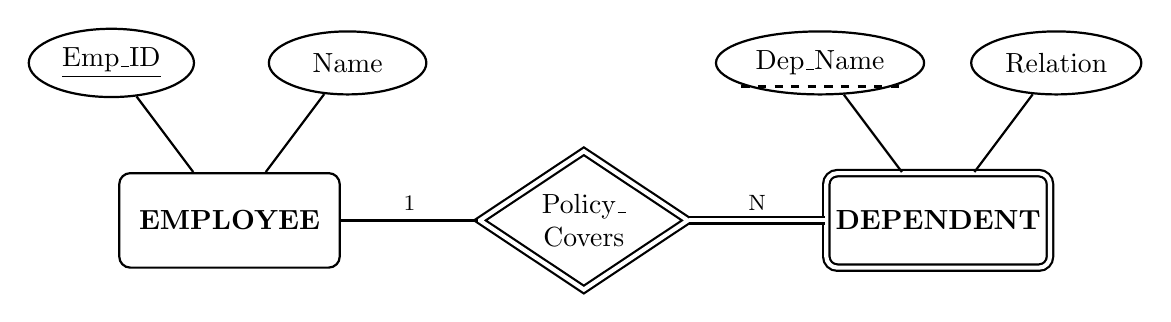
\begin{tikzpicture}[
    thick,
    entity/.style={draw, rectangle, rounded corners, minimum width=2.8cm, minimum height=1.2cm, align=center, fill=white},
    weakentity/.style={draw, double, double distance=1.5pt, rectangle, rounded corners, minimum width=2.8cm, minimum height=1.2cm, align=center, fill=white},
    relationship/.style={draw, diamond, aspect=1.5, minimum width=2.5cm, minimum height=1.2cm, align=center, fill=white},
    identrel/.style={draw, double, double distance=1.5pt, diamond, aspect=1.5, minimum width=2.5cm, minimum height=1.2cm, align=center, fill=white},
    attribute/.style={draw, ellipse, minimum width=2cm, minimum height=0.8cm, align=center, fill=white}
]
    % Entities and Relationship
    \node[entity] (emp) at (0,0) {\textbf{EMPLOYEE}};
    \node[identrel] (covers) at (4.5,0) {Policy\_\\Covers};
    \node[weakentity] (dep) at (9,0) {\textbf{DEPENDENT}};

    % Employee Attributes
    \node[attribute] (empid) at (-1.5, 2) {\underline{Emp\_ID}};
    \node[attribute] (empname) at (1.5, 2) {Name};

    % Dependent Attributes
    \node[attribute] (depname) at (7.5, 2) {Dep\_Name};
    % Manual dashed underline for partial key
    \draw[dashed, thick] (6.5, 1.7) -- (8.5, 1.7);
    
    \node[attribute] (deprel) at (10.5, 2) {Relation};

    % Connections (Attributes to Entities)
    \draw (emp) -- (empid);
    \draw (emp) -- (empname);
    
    \draw (dep) -- (depname);
    \draw (dep) -- (deprel);

    % Relationship connections with participation and cardinality
    \draw (emp) -- (covers) node[midway, above, font=\footnotesize] {1};
    \draw[double, double distance=1.5pt] (covers) -- (dep) node[midway, above, font=\footnotesize] {N};

\end{tikzpicture}
\end{center}
\vspace{1em}

\hrule
\vspace{0.75em}
\noindent\textbf{Exam Tip (Relational Mapping):} When mapping this ER model to a relational database schema, you do not create a separate table for the identifying relationship. Instead, the resulting \texttt{DEPENDENT} table will simply have the composite primary key \texttt{(Emp\_ID, Dep\_Name)}, where \texttt{Emp\_ID} acts as a foreign key referencing the \texttt{EMPLOYEE} table.

\end{tcolorbox}





\item Show an example of specialization hierarchy in the context of ERD with disjoint and overlapping subtypes.
\mk{9} \yr{CSE 303 | L-3/T-1 | 2014--15}

\begin{tcolorbox}[enhanced,breakable,ansbox,colback=cA!4,colframe=cA,boxrule=0.8pt,arc=5pt,title={\textbf{Answer}},fonttitle=\bfseries\color{white},colbacktitle=cA]

\subsection*{1. Specialization Hierarchy and Constraints}

\textbf{Specialization} is the top-down design process of defining a set of subclasses (subtypes) from a single superclass (supertype) based on distinguishing characteristics. The entities in the subtypes inherit all attributes and relationships of the supertype. 

Specialization hierarchies are governed by \textbf{disjointness constraints}, which dictate whether an entity can belong to more than one subclass simultaneously:

\begin{itemize}
    \item \textbf{Disjoint Subtypes (denoted by `d`):} An entity instance of the supertype can belong to \textbf{at most one} subtype. The subtypes are mutually exclusive.
    \item \textbf{Overlapping Subtypes (denoted by `o`):} An entity instance of the supertype can belong to \textbf{more than one} subtype simultaneously.
\end{itemize}

\subsection*{2. Example Scenario and ER Diagram}

Consider a university database containing a general \texttt{PERSON} entity. 
\begin{itemize}
    \item A \texttt{PERSON} can be a \texttt{STUDENT}, an \texttt{EMPLOYEE}, or \textbf{both}. This is an \textbf{overlapping} specialization.
    \item An \texttt{EMPLOYEE} can be either a \texttt{FACULTY} member or a \texttt{STAFF} member, but \textbf{never both}. This is a \textbf{disjoint} specialization.
    \item Furthermore, every \texttt{EMPLOYEE} \textit{must} be either \texttt{FACULTY} or \texttt{STAFF} (Total Specialization, denoted by a double line).
\end{itemize}

\vspace{1.5em}
\begin{center}
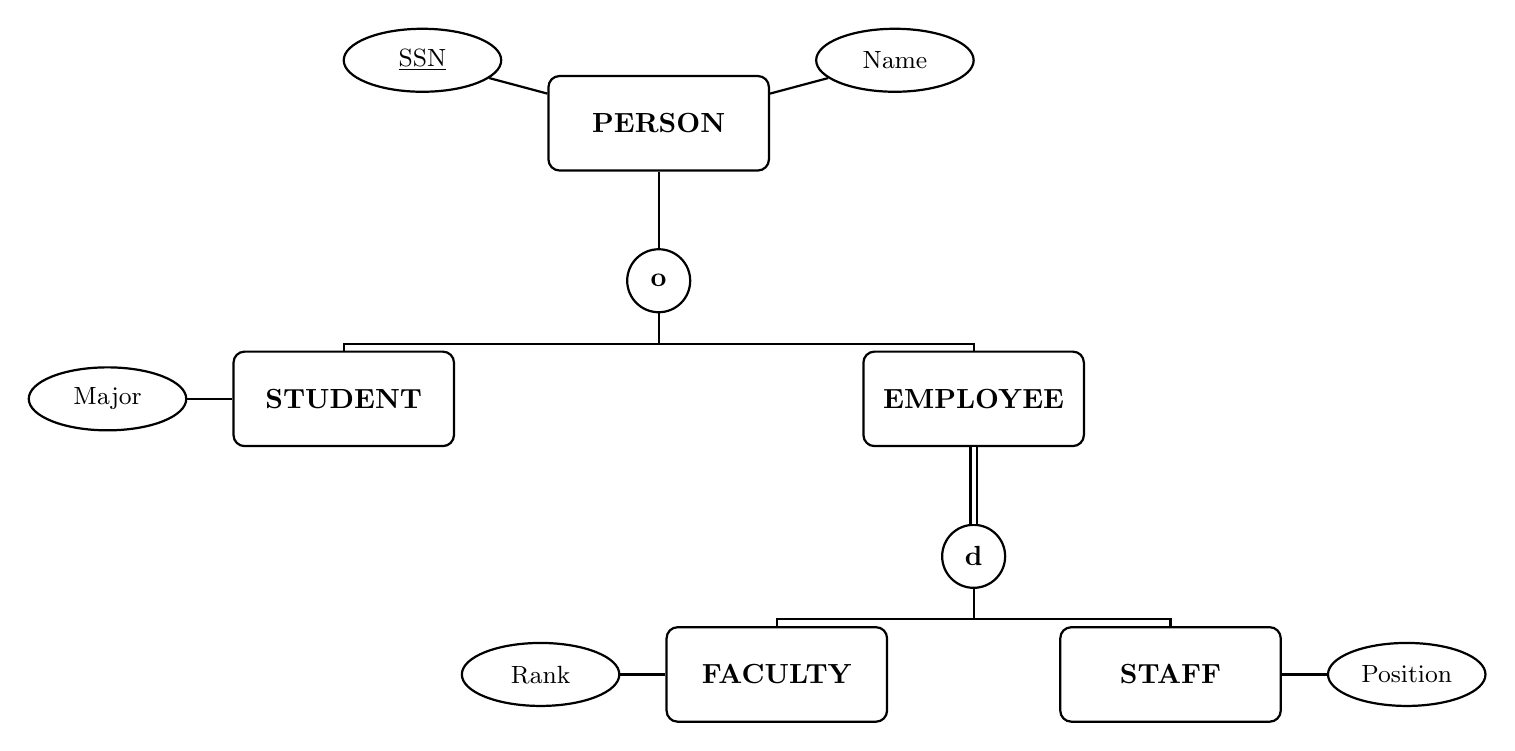
\begin{tikzpicture}[
    thick,
    entity/.style={draw, rectangle, rounded corners, minimum width=2.8cm, minimum height=1.2cm, align=center, fill=white, font=\bfseries},
    attribute/.style={draw, ellipse, minimum width=2cm, minimum height=0.8cm, align=center, fill=white, font=\small},
    spec/.style={draw, circle, minimum size=0.8cm, align=center, fill=white, font=\bfseries}
]

    % --- LEVEL 1: SUPERTYPE ---
    \node[entity] (person) at (0, 7) {PERSON};
    
    % Person Attributes
    \node[attribute] (ssn) at (-3, 7.8) {\underline{SSN}};
    \node[attribute] (name) at (3, 7.8) {Name};
    \draw (person) -- (ssn);
    \draw (person) -- (name);

    % --- LEVEL 2: OVERLAPPING SUBTYPES ---
    \node[spec] (overlap) at (0, 5) {o};
    \draw (person) -- (overlap); % Partial Specialization (Single Line)
    
    \node[entity] (student) at (-4, 3.5) {STUDENT};
    \node[entity] (employee) at (4, 3.5) {EMPLOYEE};
    
    % Connections from 'o' to Subtypes
    \draw (overlap) -- (0, 4.2) -| (student);
    \draw (overlap) -- (0, 4.2) -| (employee);
    
    % Subtype 1 Attributes
    \node[attribute] (major) at (-7, 3.5) {Major};
    \draw (student) -- (major);

    % --- LEVEL 3: DISJOINT SUBTYPES (From EMPLOYEE) ---
    \node[spec] (disjoint) at (4, 1.5) {d};
    
    % Total Specialization (Double Line)
    \draw[double, double distance=1.5pt] (employee) -- (disjoint);
    
    \node[entity] (faculty) at (1.5, 0) {FACULTY};
    \node[entity] (staff) at (6.5, 0) {STAFF};
    
    % Connections from 'd' to Subtypes
    \draw (disjoint) -- (4, 0.7) -| (faculty);
    \draw (disjoint) -- (4, 0.7) -| (staff);
    
    % Subtype 2 & 3 Attributes
    \node[attribute] (rank) at (-1.5, 0) {Rank};
    \node[attribute] (position) at (9.5, 0) {Position};
    \draw (faculty) -- (rank);
    \draw (staff) -- (position);

\end{tikzpicture}
\end{center}
\vspace{1.5em}

\subsection*{3. Key Observations from the Diagram}

\begin{enumerate}
    \item \textbf{Overlapping (`o`):} The circle containing 'o' connects \texttt{PERSON} to \texttt{STUDENT} and \texttt{EMPLOYEE}. Because it is overlapping, a specific SSN (e.g., a graduate teaching assistant) can exist simultaneously as a \texttt{STUDENT} and an \texttt{EMPLOYEE}.
    \item \textbf{Disjoint (`d`):} The circle containing 'd' connects \texttt{EMPLOYEE} to \texttt{FACULTY} and \texttt{STAFF}. An employee is strictly categorized as one or the other; no individual can hold both a standard faculty and staff role concurrently in this schema.
    \item \textbf{Completeness Constraints:}
    \begin{itemize}
        \item The single line from \texttt{PERSON} to the \texttt{`o`} circle indicates \textbf{Partial Specialization}. A \texttt{PERSON} might just be an Alumnus (not modeled here) and thus does not have to be a \texttt{STUDENT} or \texttt{EMPLOYEE}.
        \item The double line from \texttt{EMPLOYEE} to the \texttt{`d`} circle indicates \textbf{Total Specialization}. If a record exists in \texttt{EMPLOYEE}, it \textit{must} be present in either the \texttt{FACULTY} or \texttt{STAFF} subclass.
    \end{itemize}
\end{enumerate}

\end{tcolorbox}

\item Which considerations should be applied while choosing the primary key of a relation? Discuss with example how the multi-valued attribute problem in database design can be solved.
\mk{12} \yr{CSE 303 | L-3/T-1 | 2013--14}

\begin{tcolorbox}[enhanced,breakable,ansbox,colback=cA!4,colframe=cA,boxrule=0.8pt,arc=5pt,title={\textbf{Answer}},fonttitle=\bfseries\color{white},colbacktitle=cA]

\subsection*{1. Considerations for Choosing a Primary Key}

A \textbf{Primary Key (PK)} is a candidate key chosen by the database designer to uniquely identify tuples (rows) within a relation. When multiple candidate keys exist, the following considerations should be applied to select the most appropriate primary key:

\begin{itemize}
    \item \textbf{Uniqueness and Non-Nullability (Entity Integrity):} The chosen attribute(s) must guarantee uniqueness across all tuples and must never accept \texttt{NULL} values.
    \item \textbf{Irreducibility (Minimality):} If the key is composite (consisting of multiple attributes), no attribute can be removed without destroying the uniqueness property.
    \item \textbf{Immutability (Stability):} The value of a primary key should rarely, ideally never, change over time. Frequent updates to a primary key cause cascading updates in foreign keys, degrading performance and risking data anomalies.
    \item \textbf{Simplicity and Size:} A single-attribute key is preferable to a composite key. Additionally, shorter, numeric data types (e.g., \texttt{INT}) are heavily preferred over long strings (e.g., \texttt{VARCHAR}) because primary keys are heavily indexed, and smaller keys lead to faster search operations and lower storage overhead for the B+ tree indexes.
    \item \textbf{Security and Privacy:} Avoid using sensitive or personally identifiable information (PII) such as Social Security Numbers (SSN), email addresses, or phone numbers as primary keys.
    \item \textbf{Surrogate vs. Natural Keys:} If no natural candidate key meets the above criteria, a \textbf{surrogate key} (a system-generated, artificial identifier like an auto-incrementing integer) should be introduced.
\end{itemize}

\vspace{1em}
\hrule
\vspace{1em}

\subsection*{2. Solving the Multi-valued Attribute Problem}

\textbf{Definition:} A \textbf{multi-valued attribute} is an attribute that can store multiple distinct values for a single entity instance simultaneously. For example, an employee might have multiple phone numbers or possess multiple skills. 

\textbf{The Problem:} Relational databases require relations to be in \textbf{First Normal Form (1NF)}, which strictly prohibits multi-valued attributes. Storing multiple values in a single column violates atomic domains, making data retrieval, querying, and updating highly inefficient and prone to anomalies.

\textbf{The Solution:} To resolve this in database design, the multi-valued attribute is removed from the original entity and placed into a \textbf{new, separate relation}. 
\begin{itemize}
    \item The new relation contains the multi-valued attribute itself.
    \item It also includes the primary key of the original entity as a \textbf{Foreign Key (FK)}.
    \item The \textbf{Primary Key} of this new relation is the composite of the original primary key and the multi-valued attribute.
\end{itemize}

\subsubsection*{Example Scenario}
Consider an \texttt{EMPLOYEE} entity that tracks the employee's ID, Name, and multiple \texttt{Skills}. In the ER Diagram, the multi-valued attribute \texttt{Skill} is represented by a double ellipse.

\vspace{1em}
\begin{center}
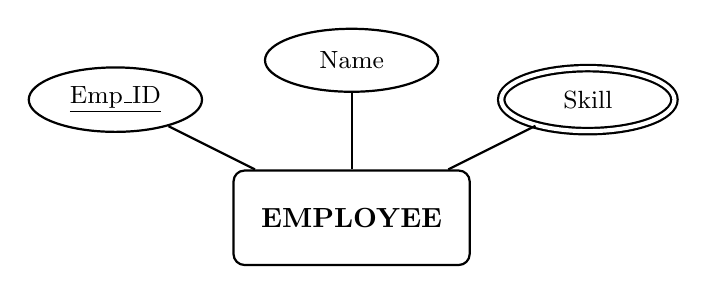
\begin{tikzpicture}[
    thick,
    entity/.style={draw, rectangle, rounded corners, minimum width=3cm, minimum height=1.2cm, align=center, fill=white, font=\bfseries},
    attribute/.style={draw, ellipse, minimum width=2.2cm, minimum height=0.8cm, align=center, fill=white, font=\small},
    multiattribute/.style={draw, double, double distance=1.5pt, ellipse, minimum width=2.2cm, minimum height=0.8cm, align=center, fill=white, font=\small}
]
    % Entity
    \node[entity] (emp) at (0,0) {EMPLOYEE};

    % Attributes
    \node[attribute] (empid) at (-3, 1.5) {\underline{Emp\_ID}};
    \node[attribute] (name) at (0, 2) {Name};
    \node[multiattribute] (skill) at (3, 1.5) {Skill};

    % Connections
    \draw (emp) -- (empid);
    \draw (emp) -- (name);
    \draw (emp) -- (skill);
\end{tikzpicture}
\end{center}
\vspace{1em}

\subsubsection*{Relational Mapping (Decomposition)}

To map this to a relational schema and conform to 1NF, we decompose the entity into two distinct tables: \texttt{EMPLOYEE} and \texttt{EMP\_SKILL}.


\vspace{1em}
\begin{center}
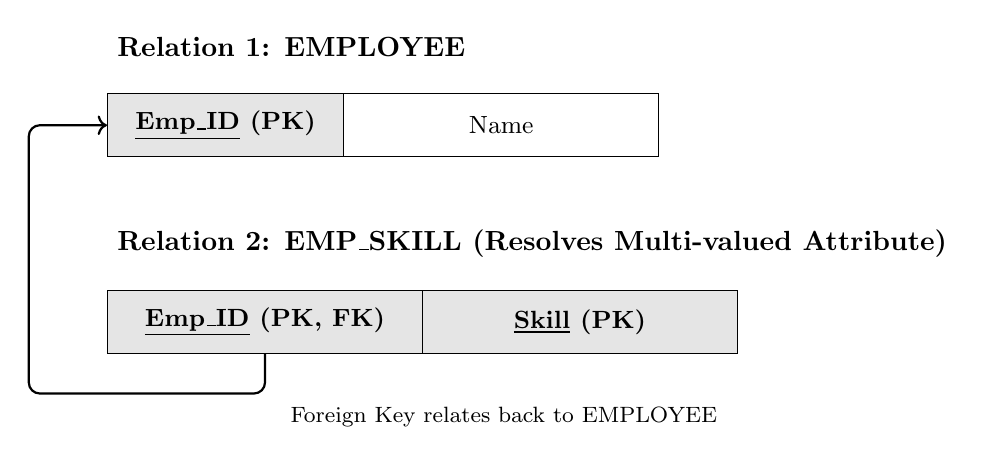
\begin{tikzpicture}[
    table/.style={draw, rectangle, minimum height=0.8cm, align=center, fill=white, font=\small},
    header/.style={table, fill=gray!20, font=\small\bfseries}
]
    % --- Table 1: EMPLOYEE ---
    \node[anchor=west, font=\bfseries] at (0, 1.5) {Relation 1: EMPLOYEE};
    
    \node[header, minimum width=3cm] (t1c1) at (1.5, 0.5) {\underline{Emp\_ID} (PK)};
    \node[table, minimum width=4cm] (t1c2) at (5, 0.5) {Name};

    % --- Table 2: EMP_SKILL ---
    \node[anchor=west, font=\bfseries] at (0, -1) {Relation 2: EMP\_SKILL (Resolves Multi-valued Attribute)};
    
    \node[header, minimum width=4cm] (t2c1) at (2, -2) {\underline{Emp\_ID} (PK, FK)};
    \node[header, minimum width=4cm] (t2c2) at (6, -2) {\underline{Skill} (PK)};

    % Foreign Key Arrow
    \draw[->, thick, rounded corners] (t2c1.south) -- ++(0,-0.5) --++(-3,0)|- (t1c1.west);
    \node[font=\footnotesize, right] at (2.2, -3.2) {Foreign Key relates back to EMPLOYEE};

\end{tikzpicture}
\end{center}

\vspace{1em}

\textbf{Explanation of the Mapping:}
\begin{enumerate}
    \item \textbf{\texttt{EMPLOYEE(Emp\_ID, Name)}:} The original entity becomes a table, holding only the single-valued attributes. \texttt{Emp\_ID} remains the Primary Key.
    \item \textbf{\texttt{EMP\_SKILL(Emp\_ID, Skill)}:} The multi-valued attribute \texttt{Skill} gets its own table. To link the skill to the correct employee, we import \texttt{Emp\_ID} as a Foreign Key. Because one employee can have many skills, \texttt{Emp\_ID} alone is not unique in this new table. Therefore, the Primary Key for \texttt{EMP\_SKILL} is the composite key \texttt{(Emp\_ID, Skill)}.
\end{enumerate}

\end{tcolorbox}

\item What are the different elements of Entity-Relation Model? Briefly discuss them.
\mk{15} \yr{CSE 303 | L-3/T-1 | 2012--13}

\begin{tcolorbox}[enhanced,breakable,ansbox,colback=cA!4,colframe=cA,boxrule=0.8pt,arc=5pt,title={\textbf{Answer}},fonttitle=\bfseries\color{white},colbacktitle=cA]

\subsection*{Introduction to the ER Model}
The \textbf{Entity-Relationship (ER) Model} is a high-level conceptual data model used in database design to represent the logical structure of a database. It abstracts the real-world system into a collection of basic objects and the associations among them. The three fundamental elements of the ER model are \textbf{Entities}, \textbf{Attributes}, and \textbf{Relationships}.

\subsection*{1. Entities and Entity Sets}
An \textbf{entity} is a real-world object or concept that exists independently and can be uniquely identified (e.g., a specific student, a specific car). An \textbf{entity set} is a collection of entities of the same type.
\begin{itemize}
    \item \textbf{Strong Entity:} An entity set that contains sufficient attributes to uniquely identify all its entities. It has a primary key and is represented by a \textbf{single rounded rectangle}.
    \item \textbf{Weak Entity:} An entity set that does not have a primary key of its own and depends on another entity (the strong entity) for its existence. It is represented by a \textbf{double rounded rectangle}.
\end{itemize}

\subsection*{2. Attributes}
\textbf{Attributes} are the properties or characteristics that describe an entity. They are represented by \textbf{ellipses}. Attributes can be classified into several types:
\begin{itemize}
    \item \textbf{Simple Attribute:} Cannot be subdivided further (e.g., Gender, Salary).
    \item \textbf{Composite Attribute:} Can be divided into smaller subparts representing basic attributes (e.g., \textit{Name} can be divided into \textit{First Name}, \textit{Middle Name}, and \textit{Last Name}).
    \item \textbf{Single-valued Attribute:} Has only a single value for a particular entity (e.g., Date of Birth).
    \item \textbf{Multi-valued Attribute:} Can have multiple values for a single entity. Represented by a \textbf{double ellipse} (e.g., Phone Number, Skills).
    \item \textbf{Derived Attribute:} Its value is computed or derived from another related attribute or set of attributes. Represented by a \textbf{dashed ellipse} (e.g., \textit{Age} derived from \textit{Date of Birth}).
    \item \textbf{Key Attribute:} Uniquely identifies an entity within an entity set. Its name is \textbf{underlined}.
\end{itemize}

\subsection*{3. Relationships and Relationship Sets}
A \textbf{relationship} is an association among two or more entities. A \textbf{relationship set} is a collection of similar relationships. They are represented by \textbf{diamonds}.
\begin{itemize}
    \item \textbf{Degree of Relationship:} The number of participating entity types (e.g., Unary, Binary, Ternary).
    \item \textbf{Cardinality Ratio:} Expresses the maximum number of relationship instances an entity can participate in (e.g., $1:1$ (One-to-One), $1:N$ (One-to-Many), $M:N$ (Many-to-Many)).
    \item \textbf{Participation Constraint:} 
    \begin{itemize}
        \item \textbf{Total Participation:} Every entity in the set must participate in at least one relationship instance. Represented by a \textbf{double line}.
        \item \textbf{Partial Participation:} Only some entities in the set participate in the relationship. Represented by a \textbf{single line}.
    \end{itemize}
    \item \textbf{Identifying Relationship:} The relationship associating a weak entity to its strong entity. Represented by a \textbf{double diamond}.
\end{itemize}

\vspace{1em}
\subsection*{4. Visual Summary of ER Elements}

The following Entity-Relationship diagram illustrates all the fundamental elements working together in a unified database schema.

\vspace{1.5em}
\begin{center}
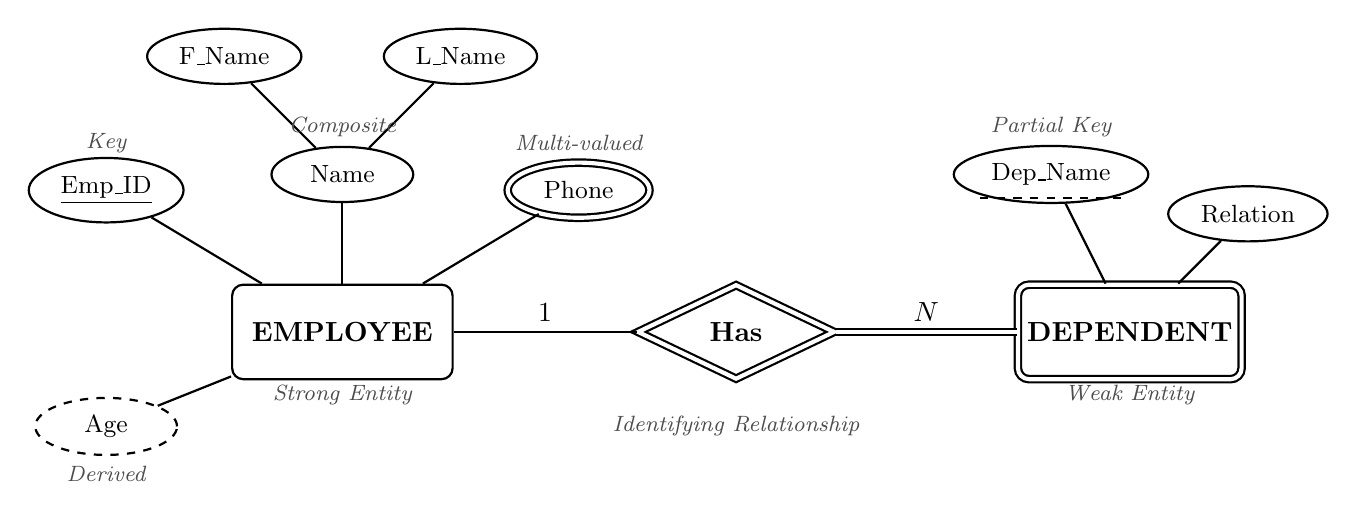
\begin{tikzpicture}[
    thick,
    entity/.style={draw, rectangle, rounded corners, minimum width=2.8cm, minimum height=1.2cm, align=center, fill=white, font=\bfseries},
    weakentity/.style={draw, double, double distance=1.5pt, rectangle, rounded corners, minimum width=2.8cm, minimum height=1.2cm, align=center, fill=white, font=\bfseries},
    relationship/.style={draw, diamond, aspect=1.5, minimum width=2.5cm, minimum height=1.2cm, align=center, fill=white, font=\bfseries},
    identrel/.style={draw, double, double distance=1.5pt, diamond, aspect=1.5, minimum width=2.5cm, minimum height=1.2cm, align=center, fill=white, font=\bfseries},
    attribute/.style={draw, ellipse, minimum width=1.8cm, minimum height=0.7cm, align=center, fill=white, font=\small},
    multiattribute/.style={draw, double, double distance=1.5pt, ellipse, minimum width=1.8cm, minimum height=0.7cm, align=center, fill=white, font=\small},
    derivedattribute/.style={draw, dashed, ellipse, minimum width=1.8cm, minimum height=0.7cm, align=center, fill=white, font=\small}
]

    % --- Entities ---
    \node[entity] (emp) at (0,0) {EMPLOYEE};
    \node[weakentity] (dep) at (10,0) {DEPENDENT};

    % --- Relationship ---
    \node[identrel] (has) at (5,0) {Has};

    % --- Connections Entity to Relationship ---
    % Employee to Has (Partial, 1)
    \draw (emp) -- (has) node[midway, above] {$1$};
    % Dependent to Has (Total, N)
    \draw[double, double distance=1.5pt] (has) -- (dep) node[midway, above] {$N$};

    % --- Employee Attributes ---
    \node[attribute] (empid) at (-3, 1.8) {\underline{Emp\_ID}};
    \node[attribute] (name) at (0, 2) {Name};
    \node[attribute] (fname) at (-1.5, 3.5) {F\_Name};
    \node[attribute] (lname) at (1.5, 3.5) {L\_Name};
    \node[multiattribute] (phone) at (3, 1.8) {Phone};
    \node[derivedattribute] (age) at (-3, -1.2) {Age};

    % Attribute Connections for Employee
    \draw (emp) -- (empid);
    \draw (emp) -- (name);
    \draw (emp) -- (phone);
    \draw (emp) -- (age);
    \draw (name) -- (fname);
    \draw (name) -- (lname);

    % --- Dependent Attributes ---
    \node[attribute] (depname) at (9, 2) {Dep\_Name};
    % Manual dashed underline for partial key
    \draw[dashed, thick] (8.1, 1.7) -- (9.9, 1.7);
    \node[attribute] (relation) at (11.5, 1.5) {Relation};

    % Attribute Connections for Dependent
    \draw (dep) -- (depname);
    \draw (dep) -- (relation);

    % --- Labels ---
    \node[font=\footnotesize\itshape, text=black!70] at (0, -0.8) {Strong Entity};
    \node[font=\footnotesize\itshape, text=black!70] at (10, -0.8) {Weak Entity};
    \node[font=\footnotesize\itshape, text=black!70] at (5, -1.2) {Identifying Relationship};
    \node[font=\footnotesize\itshape, text=black!70] at (0, 2.6) {Composite};
    \node[font=\footnotesize\itshape, text=black!70] at (-3, 2.4) {Key};
    \node[font=\footnotesize\itshape, text=black!70] at (3, 2.4) {Multi-valued};
    \node[font=\footnotesize\itshape, text=black!70] at (-3, -1.8) {Derived};
    \node[font=\footnotesize\itshape, text=black!70] at (9, 2.6) {Partial Key};

\end{tikzpicture}
\end{center}

\end{tcolorbox}

\item What is a weak entity set? What is the requirement of a weak entity set?
\mk{10} \yr{CSE 303 | L-3/T-1 | 2012--13}

\begin{tcolorbox}[enhanced,breakable,ansbox,colback=cA!4,colframe=cA,boxrule=0.8pt,arc=5pt,title={\textbf{Answer}},fonttitle=\bfseries\color{white},colbacktitle=cA]

\subsection*{1. Definition of a Weak Entity Set}
In the Entity-Relationship (ER) model, a \textbf{weak entity set} is an entity set that does not contain sufficient attributes to form a primary key of its own. Instead, it relies on another entity set—called the \textbf{strong entity set} (or owner entity set)—for its existence and identification. 

The primary key of a weak entity set is formed by a combination of the primary key of its strong entity set and its own \textbf{discriminator} (or partial key).

\subsection*{2. Requirements of a Weak Entity Set}
For a weak entity set to exist and function correctly in a database schema, the following requirements must be met:

\begin{enumerate}
    \item \textbf{Existence Dependency (Owner Entity):} A weak entity cannot exist in the database without its corresponding strong entity. If the strong entity is deleted, all its associated weak entities must also be deleted (cascading delete).
    \item \textbf{Identifying Relationship:} The weak entity set must be associated with the strong entity set via a specific relationship known as the \textbf{identifying relationship}. In an ER diagram, this is represented by a double diamond.
    \item \textbf{Total Participation:} The weak entity set must exhibit \textbf{total participation} in the identifying relationship. This means every instance of the weak entity must participate in the relationship. It is represented by a double line connecting the weak entity to the identifying relationship.
    \item \textbf{Discriminator (Partial Key):} Although it lacks a full primary key, the weak entity set must possess a set of attributes that uniquely identifies its instances \textit{among the instances related to a specific strong entity}. This attribute is called the partial key and is represented by a dashed underline in an ER diagram.
\end{enumerate}

\subsection*{3. Visual Representation (ER Diagram)}

Consider an organization where employees have dependents (e.g., children, spouse) for insurance purposes. A dependent cannot exist in the database without the employee, and two different employees might have dependents with the same name. Thus, \textbf{DEPENDENT} is a weak entity set owned by the \textbf{EMPLOYEE} strong entity set.

\vspace{1.5em}
\begin{center}
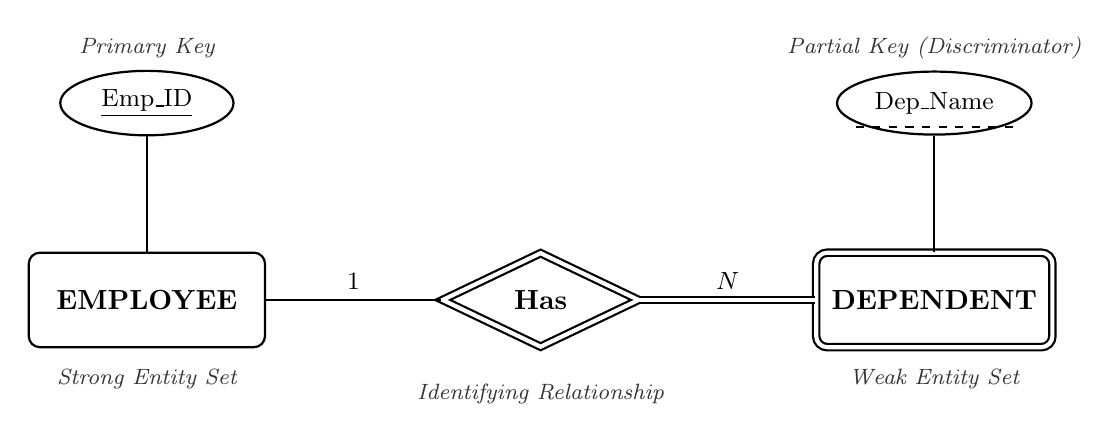
\begin{tikzpicture}[
    thick,
    entity/.style={draw, rectangle, rounded corners, minimum width=3cm, minimum height=1.2cm, align=center, fill=white, font=\bfseries},
    weakentity/.style={draw, double, double distance=1.5pt, rectangle, rounded corners, minimum width=3cm, minimum height=1.2cm, align=center, fill=white, font=\bfseries},
    identrel/.style={draw, double, double distance=1.5pt, diamond, aspect=1.5, minimum width=2.5cm, minimum height=1.2cm, align=center, fill=white, font=\bfseries},
    attribute/.style={draw, ellipse, minimum width=2.2cm, minimum height=0.8cm, align=center, fill=white, font=\small}
]

    % --- Entities ---
    \node[entity] (emp) at (0,0) {EMPLOYEE};
    \node[weakentity] (dep) at (10,0) {DEPENDENT};

    % --- Relationship ---
    \node[identrel] (has) at (5,0) {Has};

    % --- Connections Entity to Relationship ---
    % Employee to Has (Partial, Cardinality 1)
    \draw (emp) -- (has) node[midway, above, font=\small] {$1$};
    
    % Dependent to Has (Total Participation, Cardinality N)
    \draw[double, double distance=1.5pt] (has) -- (dep) node[midway, above, font=\small] {$N$};

    % --- Employee Attributes ---
    \node[attribute] (empid) at (0, 2.5) {\underline{Emp\_ID}};
    
    % Attribute Connections for Employee
    \draw (emp) -- (empid);

    % --- Dependent Attributes ---
    \node[attribute] (depname) at (10, 2.5) {Dep\_Name};
    % Manual dashed underline for partial key (Discriminator)
    \draw[dashed, thick] (9.0, 2.2) -- (11.0, 2.2);

    % Attribute Connections for Dependent
    \draw (dep) -- (depname);

    % --- Informational Labels ---
    \node[font=\footnotesize\itshape, text=black!80] at (0, -1) {Strong Entity Set};
    \node[font=\footnotesize\itshape, text=black!80] at (5, -1.2) {Identifying Relationship};
    \node[font=\footnotesize\itshape, text=black!80] at (10, -1) {Weak Entity Set};
    \node[font=\footnotesize\itshape, text=black!80] at (0, 3.2) {Primary Key};
    \node[font=\footnotesize\itshape, text=black!80] at (10, 3.2) {Partial Key (Discriminator)};

\end{tikzpicture}
\end{center}
\vspace{1em}

\subsection*{4. Comparison Summary}

\begin{center}
\renewcommand{\arraystretch}{1.3}
\begin{tabular}{@{} l p{6cm} p{6cm} @{}}
\toprule
\textbf{Feature} & \textbf{Strong Entity Set} & \textbf{Weak Entity Set} \\
\midrule
\textbf{Primary Key} & Has its own primary key. & Lacks a primary key; uses a partial key. \\
\textbf{Existence} & Exists independently. & Existence depends on a strong entity. \\
\textbf{Representation} & Single rounded rectangle. & Double rounded rectangle. \\
\textbf{Relationship} & Associated via regular relationships. & Associated via an identifying relationship (double diamond). \\
\bottomrule
\end{tabular}
\end{center}

\end{tcolorbox}

\item Consider the following scenario of a hospital:

\begin{itemize}[leftmargin=1.5em,itemsep=2pt]
  \item Patients are treated in a single ward by the doctors assigned to them. Usually each patient will be assigned a single doctor, but in rare cases he/she will be assigned two doctors.
  \item Healthcare assistants also attend to the patients; a number of these are associated with each ward.
  \item Initially the system will be concerned solely with drug treatment. Each patient is required to take a variety of drugs a certain number of times per day and for varying lengths of time.
  \item The system must record details concerning patient treatment and staff payment. Some staffs are paid on a part time basis and doctors and care assistants work varying amounts of overtime at varying rates (subject to grade).
  \item The system will also need to track what treatments are required for which patients and when, and it should be capable of calculating the cost of treatment per week for each patient.
\end{itemize}

Define entities and their attributes for the hospital management system described above.
\mk{10} \yr{CSE 303 | L-3/T-1 | 2010--11}

\begin{tcolorbox}[enhanced,breakable,ansbox,colback=cA!4,colframe=cA,boxrule=0.8pt,arc=5pt,title={\textbf{Answer}},fonttitle=\bfseries\color{white},colbacktitle=cA]

\subsection*{1. Entity Definitions and Attributes}

Based on the hospital scenario provided, the system can be modeled using the following core entities and their attributes. \textbf{Primary Keys (PK)} are underlined and used to uniquely identify records, while \textbf{Foreign Keys (FK)} establish relationships between the entities.

\begin{itemize}[leftmargin=2em, itemsep=1em]
    \item \textbf{WARD}: Represents the physical wards where patients are admitted.
    \begin{itemize}[label={--}, itemsep=2pt]
        \item \underline{\textbf{Ward\_ID}} (PK): Unique identifier for the ward.
        \item \textbf{Ward\_Name}: Name or designation of the ward.
        \item \textbf{Capacity}: Maximum number of patients the ward can hold.
    \end{itemize}

    \item \textbf{PATIENT}: Stores information regarding the individuals receiving care.
    \begin{itemize}[label={--}, itemsep=2pt]
        \item \underline{\textbf{Patient\_ID}} (PK): Unique identifier for the patient.
        \item \textbf{Name}: Full name of the patient.
        \item \textbf{Admission\_Date}: Date the patient was admitted.
        \item \textbf{Ward\_ID} (FK): The specific ward to which the patient is admitted.
    \end{itemize}

    \item \textbf{STAFF}: A generalized entity representing both doctors and healthcare assistants to streamline the payment and shift tracking system.
    \begin{itemize}[label={--}, itemsep=2pt]
        \item \underline{\textbf{Staff\_ID}} (PK): Unique identifier for the staff member.
        \item \textbf{Name}: Full name of the staff member.
        \item \textbf{Role}: Distinguishes between 'Doctor' and 'Healthcare Assistant'.
        \item \textbf{Employment\_Type}: Indicates if the staff is 'Full-time' or 'Part-time'.
        \item \textbf{Overtime\_Hours}: Tracks varying amounts of overtime worked.
        \item \textbf{Grade\_ID} (FK): Links to the pay grade for rate calculations.
    \end{itemize}

    \item \textbf{PAY\_GRADE}: Manages the varying payment rates subject to a staff member's grade.
    \begin{itemize}[label={--}, itemsep=2pt]
        \item \underline{\textbf{Grade\_ID}} (PK): Unique identifier for the pay grade.
        \item \textbf{Basic\_Hourly\_Rate}: Standard rate of pay.
        \item \textbf{Overtime\_Rate}: Multiplier or specific rate for overtime hours.
    \end{itemize}

    \item \textbf{DRUG}: Stores the inventory and pricing of treatments.
    \begin{itemize}[label={--}, itemsep=2pt]
        \item \underline{\textbf{Drug\_ID}} (PK): Unique identifier for the medication.
        \item \textbf{Drug\_Name}: Name of the drug.
        \item \textbf{Unit\_Cost}: The cost per single administration/pill of the drug.
    \end{itemize}

    \item \textbf{TREATMENT}: An associative entity (or relationship entity) tracking the specific drug regimens assigned to patients.
    \begin{itemize}[label={--}, itemsep=2pt]
        \item \underline{\textbf{Treatment\_ID}} (PK): Unique identifier for the specific treatment plan.
        \item \textbf{Patient\_ID} (FK): The patient receiving the treatment.
        \item \textbf{Drug\_ID} (FK): The specific drug prescribed.
        \item \textbf{Doctor\_ID} (FK): The staff ID of the doctor who prescribed it.
        \item \textbf{Frequency\_Per\_Day}: Number of times the drug must be taken daily.
        \item \textbf{Duration\_Days}: Varying length of time the drug is required.
        \item \textit{\textbf{Weekly\_Cost}} (Derived): A calculated attribute resolving the system's need to compute treatment cost per week ($\text{Frequency\_Per\_Day} \times 7 \times \text{Unit\_Cost}$).
    \end{itemize}
    
    \item \textbf{PATIENT\_DOCTOR\_ASSIGNMENT}: Resolves the many-to-many relationship mapping between patients and their assigned doctors (as a patient can have 1 or 2 doctors).
    \begin{itemize}[label={--}, itemsep=2pt]
        \item \underline{\textbf{Patient\_ID}} (PK, FK)
        \item \underline{\textbf{Staff\_ID}} (PK, FK)
    \end{itemize}
\end{itemize}

\vspace{1.5em}
\subsection*{2. Conceptual Entity-Relationship (ER) Diagram}

The following diagram illustrates the core entities, their key attributes, and the cardinalities of their relationships based on the constraints described in the scenario.

\vspace{2em}
\begin{center}
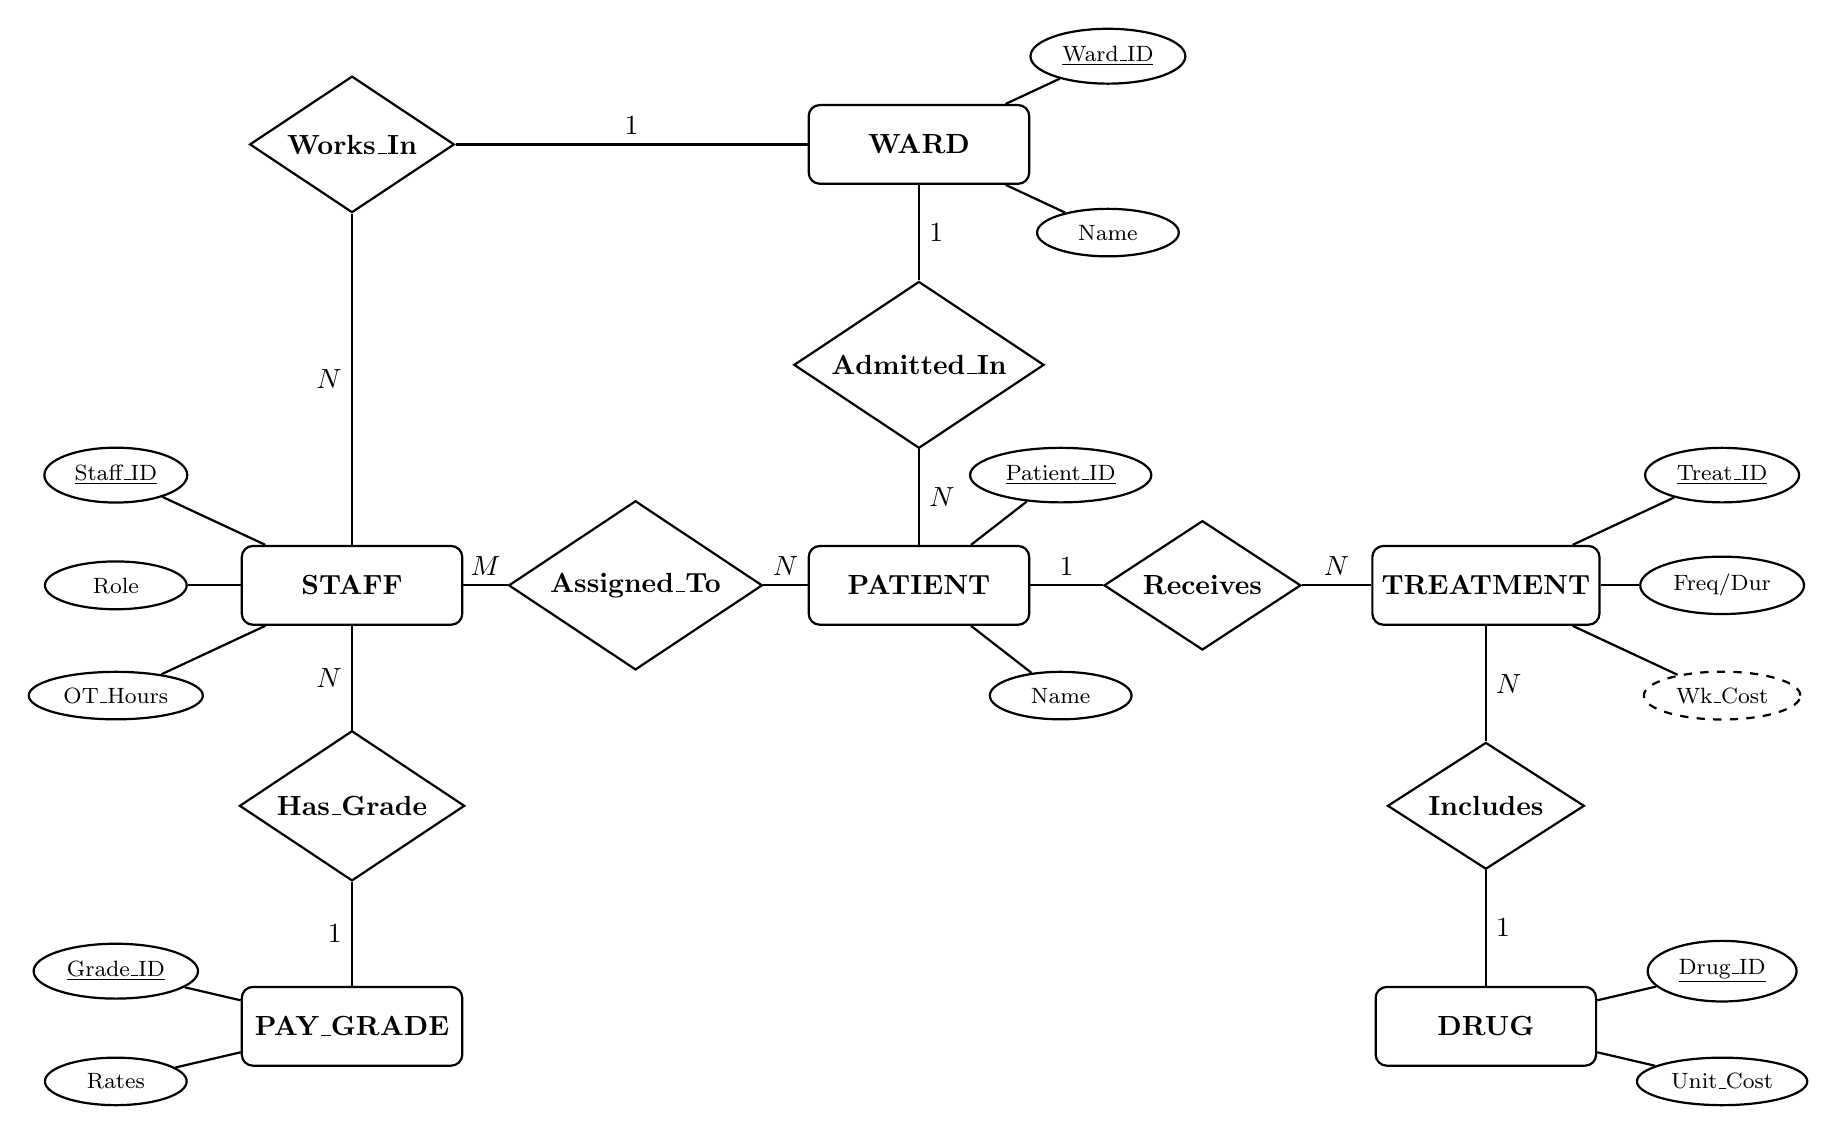
\begin{tikzpicture}[
    thick,x=1.2cm,y=1.4cm, 
    node distance=2.5cm,
    entity/.style={draw, rectangle, rounded corners, minimum width=2.8cm, minimum height=1cm, align=center, fill=white, font=\bfseries},
    relationship/.style={draw, diamond, aspect=1.5, minimum width=2.5cm, minimum height=1cm, align=center, fill=white, font=\bfseries},
    attribute/.style={draw, ellipse, minimum width=1.8cm, minimum height=0.6cm, align=center, fill=white, font=\footnotesize},
    derived/.style={draw, dashed, ellipse, minimum width=1.8cm, minimum height=0.6cm, align=center, fill=white, font=\footnotesize}
]

    % --- Entities ---
    \node[entity] (patient) at (0, 0) {PATIENT};
    \node[entity] (ward) at (0, 4) {WARD};
    \node[entity] (staff) at (-6, 0) {STAFF};
    \node[entity] (grade) at (-6, -4) {PAY\_GRADE};
    \node[entity] (treatment) at (6, 0) {TREATMENT};
    \node[entity] (drug) at (6, -4) {DRUG};

    % --- Relationships ---
    \node[relationship] (admitted) at (0, 2) {Admitted\_In};
    \node[relationship] (treats) at (-3, 0) {Assigned\_To}; % Doctor to Patient
    \node[relationship] (assigned) at (-6, 4) {Works\_In}; % Assistant to Ward
    \node[relationship] (hasgrade) at (-6, -2) {Has\_Grade};
    \node[relationship] (receives) at (3, 0) {Receives};
    \node[relationship] (includes) at (6, -2) {Includes};

    % --- Connecting Entities and Relationships with Cardinalities ---
    \draw (patient) -- (admitted) node[midway, right] {$N$};
    \draw (admitted) -- (ward) node[midway, right] {$1$};

    \draw (staff) -- (treats) node[midway, above] {$M$};
    \draw (treats) -- (patient) node[midway, above] {$N$};

    \draw (staff) -- (assigned) node[midway, left] {$N$};
    \draw (assigned) -- (ward) node[midway, above] {$1$};

    \draw (staff) -- (hasgrade) node[midway, left] {$N$};
    \draw (hasgrade) -- (grade) node[midway, left] {$1$};

    \draw (patient) -- (receives) node[midway, above] {$1$};
    \draw (receives) -- (treatment) node[midway, above] {$N$};

    \draw (treatment) -- (includes) node[midway, right] {$N$};
    \draw (includes) -- (drug) node[midway, right] {$1$};

    % --- Attributes for WARD ---
    \node[attribute] (wardid) at (2, 4.8) {\underline{Ward\_ID}};
    \node[attribute] (wname) at (2, 3.2) {Name};
    \draw (ward) -- (wardid); \draw (ward) -- (wname);

    % --- Attributes for PATIENT ---
    \node[attribute] (patid) at (1.5, 1) {\underline{Patient\_ID}};
    \node[attribute] (pname) at (1.5, -1) {Name};
    \draw (patient) -- (patid); \draw (patient) -- (pname);

    % --- Attributes for STAFF ---
    \node[attribute] (staffid) at (-8.5, 1) {\underline{Staff\_ID}};
    \node[attribute] (srole) at (-8.5, 0) {Role};
    \node[attribute] (sot) at (-8.5, -1) {OT\_Hours};
    \draw (staff) -- (staffid); \draw (staff) -- (srole); \draw (staff) -- (sot);

    % --- Attributes for PAY_GRADE ---
    \node[attribute] (gradeid) at (-8.5, -3.5) {\underline{Grade\_ID}};
    \node[attribute] (grates) at (-8.5, -4.5) {Rates};
    \draw (grade) -- (gradeid); \draw (grade) -- (grates);

    % --- Attributes for TREATMENT ---
    \node[attribute] (treatid) at (8.5, 1) {\underline{Treat\_ID}};
    \node[attribute] (tfreq) at (8.5, 0) {Freq/Dur};
    \node[derived] (tcost) at (8.5, -1) {Wk\_Cost};
    \draw (treatment) -- (treatid); \draw (treatment) -- (tfreq); \draw (treatment) -- (tcost);

    % --- Attributes for DRUG ---
    \node[attribute] (drugid) at (8.5, -3.5) {\underline{Drug\_ID}};
    \node[attribute] (dcost) at (8.5, -4.5) {Unit\_Cost};
    \draw (drug) -- (drugid); \draw (drug) -- (dcost);

\end{tikzpicture}
\end{center}



\end{tcolorbox}

\end{enumerate}

%%──────────────────────────────────────────────────────────────────────
\subtopic{cA}{ER Diagrams}
\label{sub:s2-erdiag}

\begin{enumerate}


\item You are the manager of the website development department of your organisation.
Each website developed by your organization can be uniquely identified by a url. It also has
a public host-ip address and a date of going live. Each website is developed by a team of
developers. Each developer can be uniquely identified by an employee id. The relevant information
for a developer is his/her name, address, highest educational qualification, salary
and hire date. Each website is developed by a web-based framework which is associated
with a particular programming language. Each framework and its associated programming
language have a specific name and the development year. The other information relevant
to a web framework is its author name.

Design an Entity-Relationship Diagram for your website development department to manage it conveniently. 
\mk{10} \yr{CSE 215 | L-2/T-2 | 2018--19}

\begin{tcolorbox}[enhanced,breakable,ansbox,colback=cA!4,colframe=cA,boxrule=0.8pt,arc=5pt,title={\textbf{Answer}},fonttitle=\bfseries\color{white},colbacktitle=cA]

\subsection*{1. Entity Identification and Attributes}
Based on the provided scenario for the website development department, we can identify four primary entities along with their respective attributes. \textbf{Primary Keys (PK)} are used to uniquely identify each record.

\begin{itemize}[leftmargin=2em, itemsep=0.5em]
    \item \textbf{WEBSITE}: Stores details about the deployed projects.
    \begin{itemize}[label={--}, itemsep=1pt]
        \item \underline{\textbf{URL}} (PK): The unique identifier for each website.
        \item \textbf{Host\_IP}: The public host-IP address.
        \item \textbf{Live\_Date}: The date the website went live.
    \end{itemize}

    \item \textbf{DEVELOPER}: Stores professional and personal details of the staff.
    \begin{itemize}[label={--}, itemsep=1pt]
        \item \underline{\textbf{Emp\_ID}} (PK): The unique employee identifier.
        \item \textbf{Name}: The full name of the developer.
        \item \textbf{Address}: Residential address.
        \item \textbf{Qualification}: Highest educational qualification.
        \item \textbf{Salary}: Current compensation.
        \item \textbf{Hire\_Date}: Date of joining the organization.
    \end{itemize}

    \item \textbf{FRAMEWORK}: Details the web-based frameworks utilized for development.
    \begin{itemize}[label={--}, itemsep=1pt]
        \item \underline{\textbf{F\_Name}} (PK): The specific name of the framework.
        \item \textbf{F\_Dev\_Year}: The year the framework was developed.
        \item \textbf{Author}: The author or creator of the framework.
    \end{itemize}

    \item \textbf{LANGUAGE}: The programming language associated with the frameworks.
    \begin{itemize}[label={--}, itemsep=1pt]
        \item \underline{\textbf{L\_Name}} (PK): The specific name of the programming language.
        \item \textbf{L\_Dev\_Year}: The development year of the language.
    \end{itemize}
\end{itemize}

\subsection*{2. Relationships and Cardinalities}
The entities interact through the following relationships:
\begin{itemize}
    \item \textbf{Develops (DEVELOPER and WEBSITE)}: A \textbf{Many-to-Many (M:N)} relationship. The scenario states a website is developed by a "team of developers" (meaning multiple developers per website), and a developer can generally work on multiple websites over time. 
    \item \textbf{Uses\_Framework (WEBSITE and FRAMEWORK)}: A \textbf{Many-to-One (N:1)} relationship. Each website is developed using one specific web-based framework, but a single framework can be used to build many websites.
    \item \textbf{Associated\_With (FRAMEWORK and LANGUAGE)}: A \textbf{Many-to-One (N:1)} relationship. Each framework is associated with a \textit{particular} (single) programming language, while a programming language (like Python or JavaScript) can have multiple frameworks associated with it (e.g., Django, Flask).
\end{itemize}

\vspace{1em}
\subsection*{3. Entity-Relationship (ER) Diagram}

\begin{center}
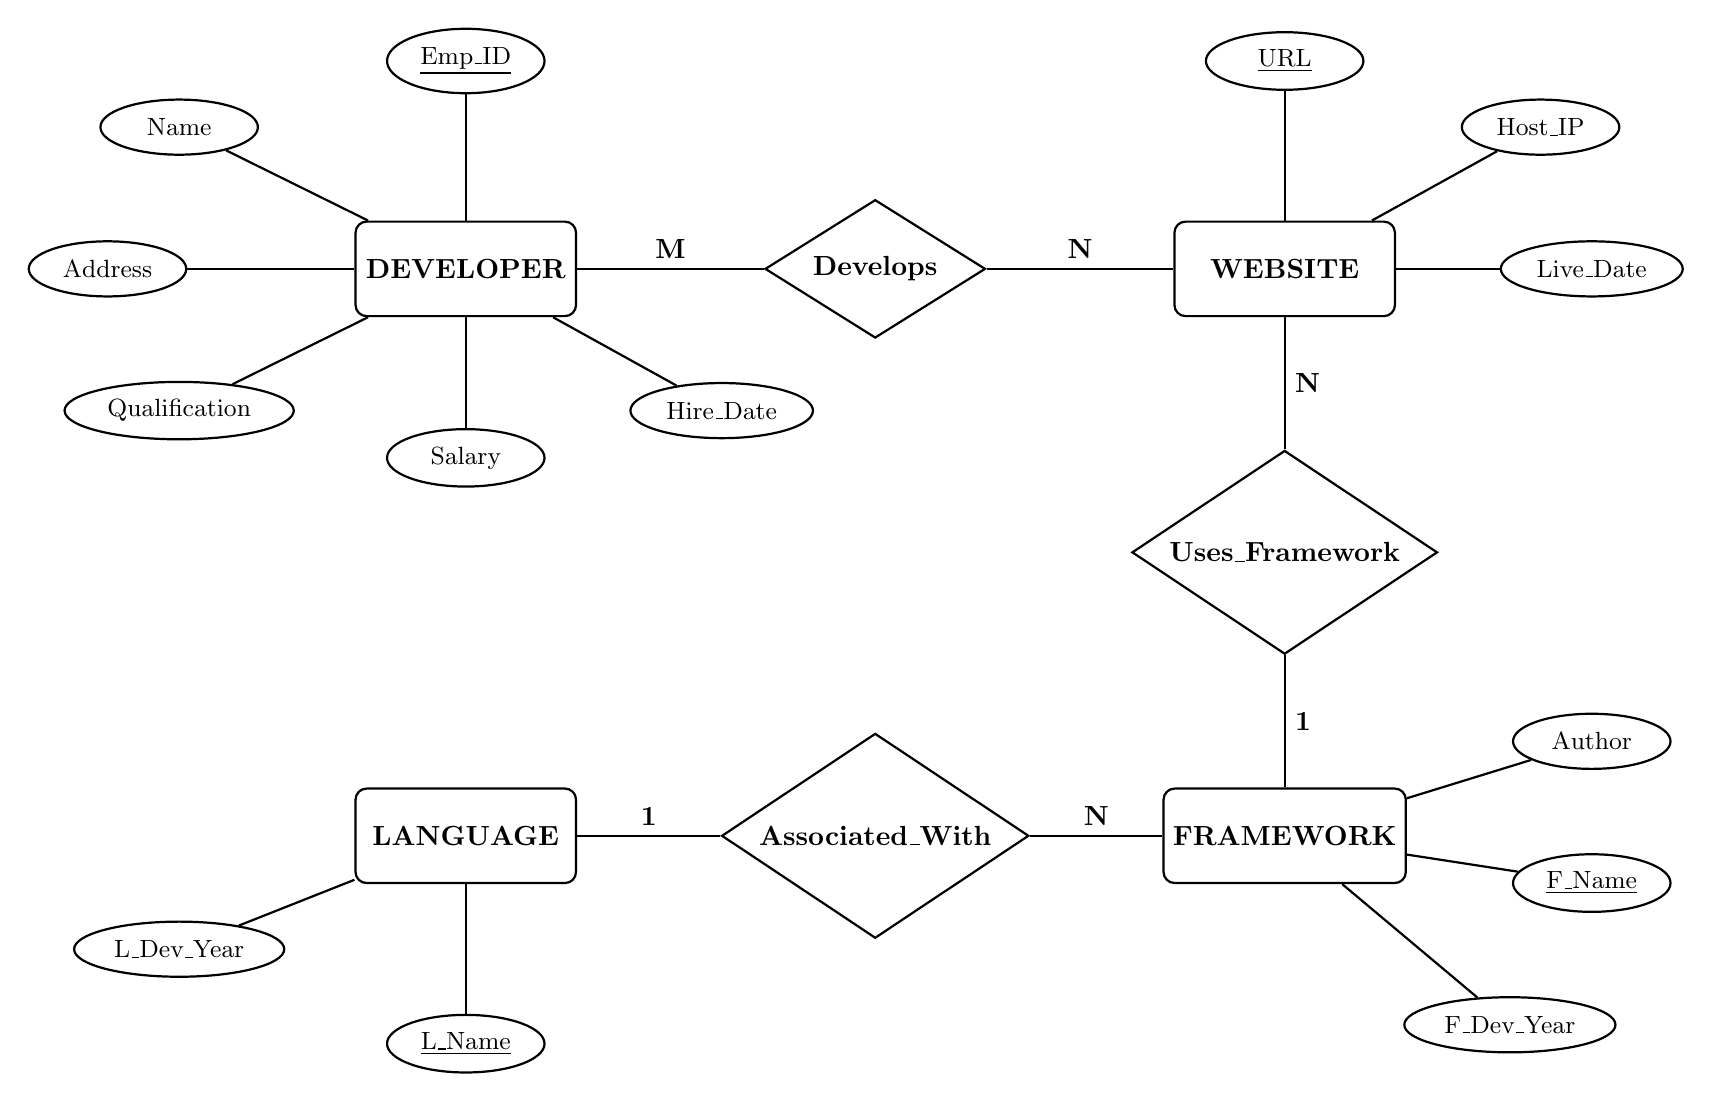
\begin{tikzpicture}[
    thick,x=1.3cm,y=1.2cm,
    entity/.style={draw, rectangle, rounded corners, minimum width=2.8cm, minimum height=1.2cm, align=center, fill=white, font=\bfseries},
    relationship/.style={draw, diamond, aspect=1.5, minimum width=2.8cm, minimum height=1.2cm, align=center, fill=white, font=\bfseries},
    attribute/.style={draw, ellipse, minimum width=2cm, minimum height=0.7cm, align=center, fill=white, font=\small}
]

    % --- Entities ---
    \node[entity] (DEV) at (-4, 3) {DEVELOPER};
    \node[entity] (WEB) at (4, 3) {WEBSITE};
    \node[entity] (FWK) at (4, -3) {FRAMEWORK};
    \node[entity] (LANG) at (-4, -3) {LANGUAGE};

    % --- Relationships ---
    \node[relationship] (DEV_WEB) at (0, 3) {Develops};
    \node[relationship] (WEB_FWK) at (4, 0) {Uses\_Framework};
    \node[relationship] (FWK_LANG) at (0, -3) {Associated\_With};

    % --- Connection Lines & Cardinalities ---
    \draw (DEV) -- (DEV_WEB) node[midway, above, font=\bfseries] {M};
    \draw (DEV_WEB) -- (WEB) node[midway, above, font=\bfseries] {N};

    \draw (WEB) -- (WEB_FWK) node[midway, right, font=\bfseries] {N};
    \draw (WEB_FWK) -- (FWK) node[midway, right, font=\bfseries] {1};

    \draw (FWK) -- (FWK_LANG) node[midway, above, font=\bfseries] {N};
    \draw (FWK_LANG) -- (LANG) node[midway, above, font=\bfseries] {1};

    % --- Attributes for DEVELOPER ---
    \node[attribute] (d_id) at (-4, 5.2) {\underline{Emp\_ID}};
    \node[attribute] (d_name) at (-6.8, 4.5) {Name};
    \node[attribute] (d_addr) at (-7.5, 3) {Address};
    \node[attribute] (d_qual) at (-6.8, 1.5) {Qualification};
    \node[attribute] (d_sal) at (-4, 1) {Salary};
    \node[attribute] (d_hire) at (-1.5, 1.5) {Hire\_Date};

    \draw (DEV) -- (d_id);
    \draw (DEV) -- (d_name);
    \draw (DEV) -- (d_addr);
    \draw (DEV) -- (d_qual);
    \draw (DEV) -- (d_sal);
    \draw (DEV) -- (d_hire);

    % --- Attributes for WEBSITE ---
    \node[attribute] (w_url) at (4, 5.2) {\underline{URL}};
    \node[attribute] (w_ip) at (6.5, 4.5) {Host\_IP};
    \node[attribute] (w_date) at (7, 3) {Live\_Date};

    \draw (WEB) -- (w_url);
    \draw (WEB) -- (w_ip);
    \draw (WEB) -- (w_date);

    % --- Attributes for FRAMEWORK ---
    \node[attribute] (f_author) at (7, -2) {Author};
    \node[attribute] (f_name) at (7, -3.5) {\underline{F\_Name}};
    \node[attribute] (f_year) at (6.2, -5) {F\_Dev\_Year};

    \draw (FWK) -- (f_author);
    \draw (FWK) -- (f_name);
    \draw (FWK) -- (f_year);

    % --- Attributes for LANGUAGE ---
    \node[attribute] (l_name) at (-4, -5.2) {\underline{L\_Name}};
    \node[attribute] (l_year) at (-6.8, -4.2) {L\_Dev\_Year};

    \draw (LANG) -- (l_name);
    \draw (LANG) -- (l_year);

\end{tikzpicture}
\end{center}


\end{tcolorbox}

\item You are designing a database for a university with the following requirements: Each student has a student id, name, address and contact name. Each course has a course number, name, credit hours, and the minimum level and term. Each student enrols in several courses. University employees are either faculty members or office staff. Faculty members have a name, designation, address, contact number and room number. Office staff have a name, contact, address and hourly payment rate. In each semester (identified by a label e.g.\ ``January 2019''), every faculty member conducts several courses; a single course can have many teachers. If a course is conducted by several teachers, one is assigned as coordinator.
\begin{enumerate}
  \item Write down the list of entity sets with their attributes.
  \item Draw the E/R diagram using appropriate arrows to indicate multiplicity. Show attributes on relations where applicable.
\end{enumerate}
\mk{20} \yr{CSE 215 | L-2/T-2 | 2017--18}

\begin{tcolorbox}[enhanced,breakable,ansbox,colback=cA!4,colframe=cA,boxrule=0.8pt,arc=5pt,title={\textbf{Answer}},fonttitle=\bfseries\color{white},colbacktitle=cA]

\subsection*{1. Entity Sets and their Attributes}

Based on the scenario, we can identify the following entity sets and their attributes. A generalized superclass \textbf{EMPLOYEE} is introduced to hold the shared attributes of \textbf{FACULTY} and \textbf{OFFICE\_STAFF}. Primary keys are underlined.

\begin{itemize}[leftmargin=2em, itemsep=0.5em]
    \item \textbf{STUDENT}: \underline{Student\_ID}, Name, Address, Contact\_Name.
    \item \textbf{COURSE}: \underline{Course\_No}, Name, Credit\_Hours, Min\_Level, Min\_Term.
    \item \textbf{EMPLOYEE} (Superclass): \underline{Emp\_ID} (Assumed as a unique identifier), Name, Address, Contact\_Number.
    \item \textbf{FACULTY} (Subclass of Employee): Designation, Room\_Number.
    \item \textbf{OFFICE\_STAFF} (Subclass of Employee): Hourly\_Rate.
\end{itemize}

\textbf{Relationship Sets \& their Attributes:}
\begin{itemize}[leftmargin=2em, itemsep=0.5em]
    \item \textbf{Enrols}: Associates \textbf{STUDENT} and \textbf{COURSE}. (Multiplicity: Many-to-Many).
    \item \textbf{Conducts}: Associates \textbf{FACULTY} and \textbf{COURSE}. (Multiplicity: Many-to-Many). 
    \begin{itemize}
        \item \textit{Attributes}: \textbf{Semester} (label indicating when it is taught), \textbf{Is\_Coordinator} (Boolean flag indicating if the faculty is the assigned coordinator for that course).
    \end{itemize}
\end{itemize}

\vspace{1em}
\subsection*{2. Entity-Relationship (ER) Diagram}

The following ER diagram uses standard Chen's notation. The generalization (ISA) is represented by a circle linking the subclasses to the superclass.

\vspace{1.5em}
\begin{center}
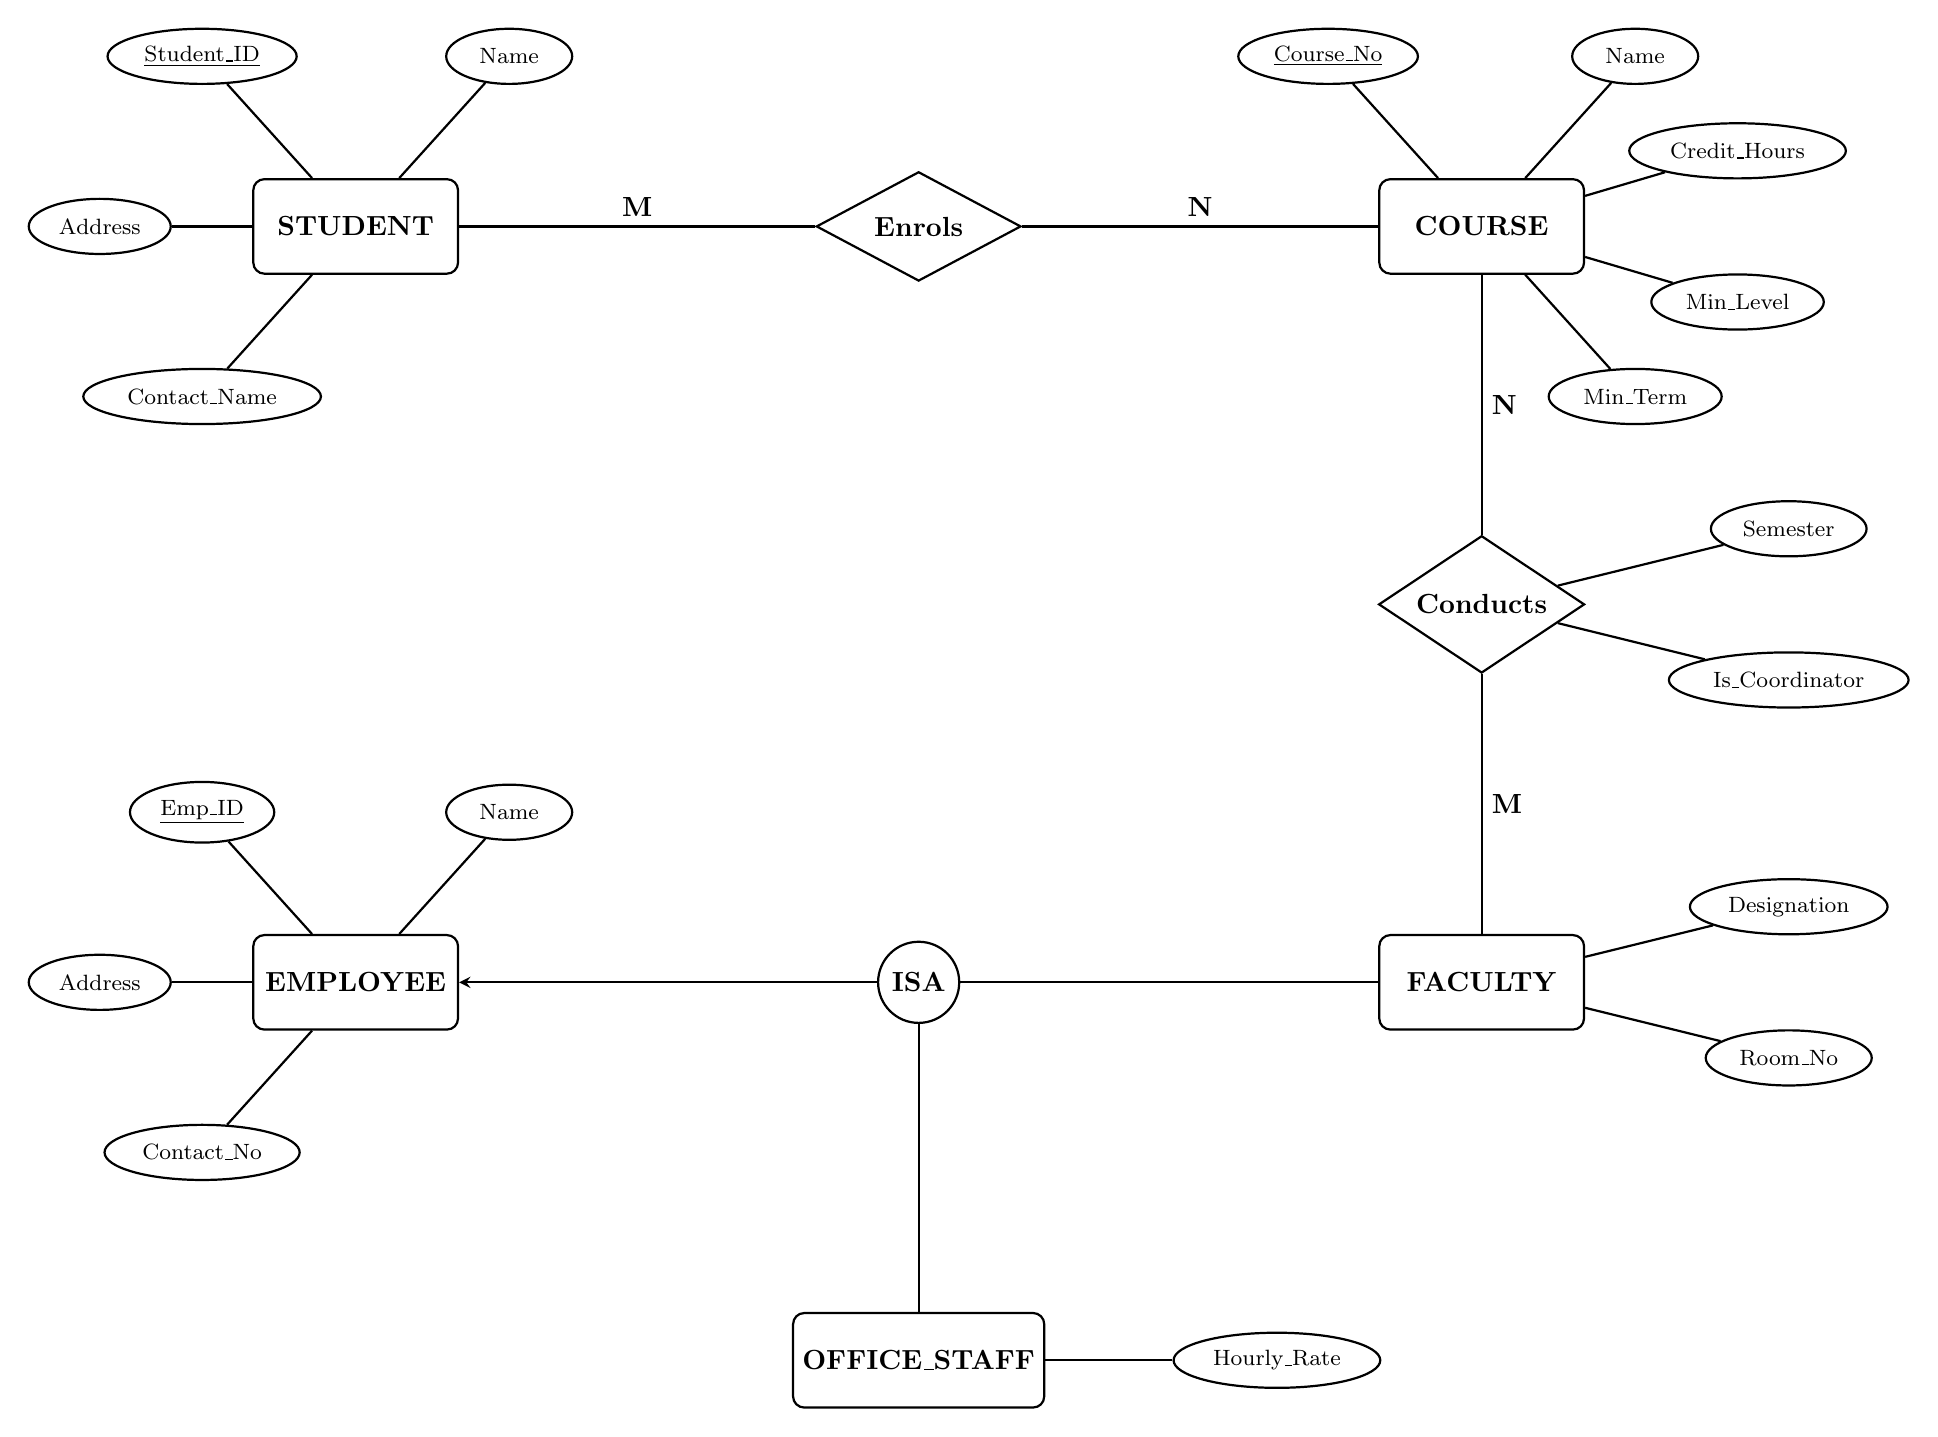
\begin{tikzpicture}[
    thick,x=1.3cm, y=1.2cm,
    entity/.style={draw, rectangle, rounded corners, minimum width=2.6cm, minimum height=1.2cm, align=center, fill=white, font=\bfseries},
    relationship/.style={draw, diamond, aspect=1.5, minimum width=2.6cm, minimum height=1.2cm, align=center, fill=white, font=\bfseries},
    attribute/.style={draw, ellipse, minimum width=1.6cm, minimum height=0.7cm, align=center, fill=white, font=\footnotesize},
    isa/.style={draw, circle, minimum size=1cm, align=center, fill=white, font=\bfseries}
]

    % ================= ENTITIES =================
    \node[entity] (STUDENT) at (-6, 4) {STUDENT};
    \node[entity] (COURSE) at (5, 4) {COURSE};
    \node[entity] (EMPLOYEE) at (-6, -4) {EMPLOYEE};
    \node[entity] (FACULTY) at (5, -4) {FACULTY};
    \node[entity] (STAFF) at (-0.5, -8) {OFFICE\_STAFF};

    % ================= RELATIONSHIPS & ISA =================
    \node[relationship] (ENROLS) at (-0.5, 4) {Enrols};
    \node[relationship] (CONDUCTS) at (5, 0) {Conducts};
    \node[isa] (ISA) at (-0.5, -4) {ISA};

    % ================= CONNECTIONS WITH MULTIPLICITIES =================
    % Student - Enrols - Course
    \draw (STUDENT) -- (ENROLS) node[midway, above, font=\bfseries] {M};
    \draw (ENROLS) -- (COURSE) node[midway, above, font=\bfseries] {N};

    % Faculty - Conducts - Course
    \draw (FACULTY) -- (CONDUCTS) node[midway, right, font=\bfseries] {M};
    \draw (CONDUCTS) -- (COURSE) node[midway, right, font=\bfseries] {N};

    % Employee Hierarchy (ISA)
    \draw[->, >=stealth] (ISA) -- (EMPLOYEE); % Arrow pointing to Superclass
    \draw (FACULTY) -- (ISA);
    \draw (STAFF) -- (ISA);

    % ================= ATTRIBUTES =================
    
    % --- STUDENT Attributes ---
    \node[attribute] (s_id) at (-7.5, 5.8) {\underline{Student\_ID}};
    \node[attribute] (s_name) at (-4.5, 5.8) {Name};
    \node[attribute] (s_addr) at (-8.5, 4) {Address};
    \node[attribute] (s_contact) at (-7.5, 2.2) {Contact\_Name};
    
    \draw (STUDENT) -- (s_id);
    \draw (STUDENT) -- (s_name);
    \draw (STUDENT) -- (s_addr);
    \draw (STUDENT) -- (s_contact);

    % --- COURSE Attributes ---
    \node[attribute] (c_no) at (3.5, 5.8) {\underline{Course\_No}};
    \node[attribute] (c_name) at (6.5, 5.8) {Name};
    \node[attribute] (c_credit) at (7.5, 4.8) {Credit\_Hours};
    \node[attribute] (c_minlvl) at (7.5, 3.2) {Min\_Level};
    \node[attribute] (c_minterm) at (6.5, 2.2) {Min\_Term};

    \draw (COURSE) -- (c_no);
    \draw (COURSE) -- (c_name);
    \draw (COURSE) -- (c_credit);
    \draw (COURSE) -- (c_minlvl);
    \draw (COURSE) -- (c_minterm);

    % --- CONDUCTS Attributes ---
    \node[attribute] (cond_sem) at (8, 0.8) {Semester};
    \node[attribute] (cond_coord) at (8, -0.8) {Is\_Coordinator};

    \draw (CONDUCTS) -- (cond_sem);
    \draw (CONDUCTS) -- (cond_coord);

    % --- EMPLOYEE Attributes ---
    \node[attribute] (e_id) at (-7.5, -2.2) {\underline{Emp\_ID}};
    \node[attribute] (e_name) at (-4.5, -2.2) {Name};
    \node[attribute] (e_addr) at (-8.5, -4) {Address};
    \node[attribute] (e_contact) at (-7.5, -5.8) {Contact\_No};

    \draw (EMPLOYEE) -- (e_id);
    \draw (EMPLOYEE) -- (e_name);
    \draw (EMPLOYEE) -- (e_addr);
    \draw (EMPLOYEE) -- (e_contact);

    % --- FACULTY Attributes ---
    \node[attribute] (f_desig) at (8, -3.2) {Designation};
    \node[attribute] (f_room) at (8, -4.8) {Room\_No};

    \draw (FACULTY) -- (f_desig);
    \draw (FACULTY) -- (f_room);

    % --- OFFICE STAFF Attributes ---
    \node[attribute] (o_rate) at (3, -8) {Hourly\_Rate};

    \draw (STAFF) -- (o_rate);

\end{tikzpicture}
\end{center}

\end{tcolorbox}

\item 
There are many books in central library of BUET in different subjects. Each book must
have a ISBN number, title, name of authors, subject and number of copies. A book can
have multiple copies and each copy is identified by an accession number. The
descriptive attributes of each copy of book are edition, price and data of purchase. A
publisher publishes many books and a book is published by ofily one publisher. A
publisher is identified by publisher id and described by name, country of origin,
address and contact numbers.
Book suppliers supply many copies of books to the library by tender in each year.- A
tender has an id, name, total price and year. For each copy of books, you must store the
record of which copy of book has been supplied by which supplier in which tender. A
supplier is identified by supplier id and described by name, address and contact
numbers.
One copy of a book (book-copy) can be issued to multiple borrowers in different times
and a borrower can borrow multiple number of book-copies. Borrowers can be
teachers, students or staffs. Each borrower must have a borrower id, name, contact
number and address. Teachers are described by joining date and designation. Students
are described by session, level and term. Staffs are described by office name.
When a book-copy is issued to borrower, some information such as issued data,
accession number, borrower id, length of period for issue and return date are needed to
enter into the database. At the same time, the status of the borrowed book should be
labeled as issued and will be cleared after return by the borrower.
\begin{enumerate}
  \item Draw an ERD for the above library management system.
  \item Transform the ERD into tables showing all primary keys and foreign keys.
\end{enumerate}
\mk{35} \yr{CSE 303 | L-3/T-1 | 2016--17}

\begin{tcolorbox}[enhanced,breakable,ansbox,colback=cA!4,colframe=cA,boxrule=0.8pt,arc=5pt,title={\textbf{Answer}},fonttitle=\bfseries\color{white},colbacktitle=cA]

\subsection*{1. Entity-Relationship Diagram (ERD)}

The following Entity-Relationship Diagram models the library management system. A generalized \textbf{BORROWER} superclass is used to represent \textbf{TEACHER}, \textbf{STUDENT}, and \textbf{STAFF}. A ternary relationship \textbf{Supplies} links \textbf{SUPPLIER}, \textbf{TENDER}, and \textbf{BOOK\_COPY}.

\vspace{1em}
\begin{center}
\resizebox{\textwidth}{!}{
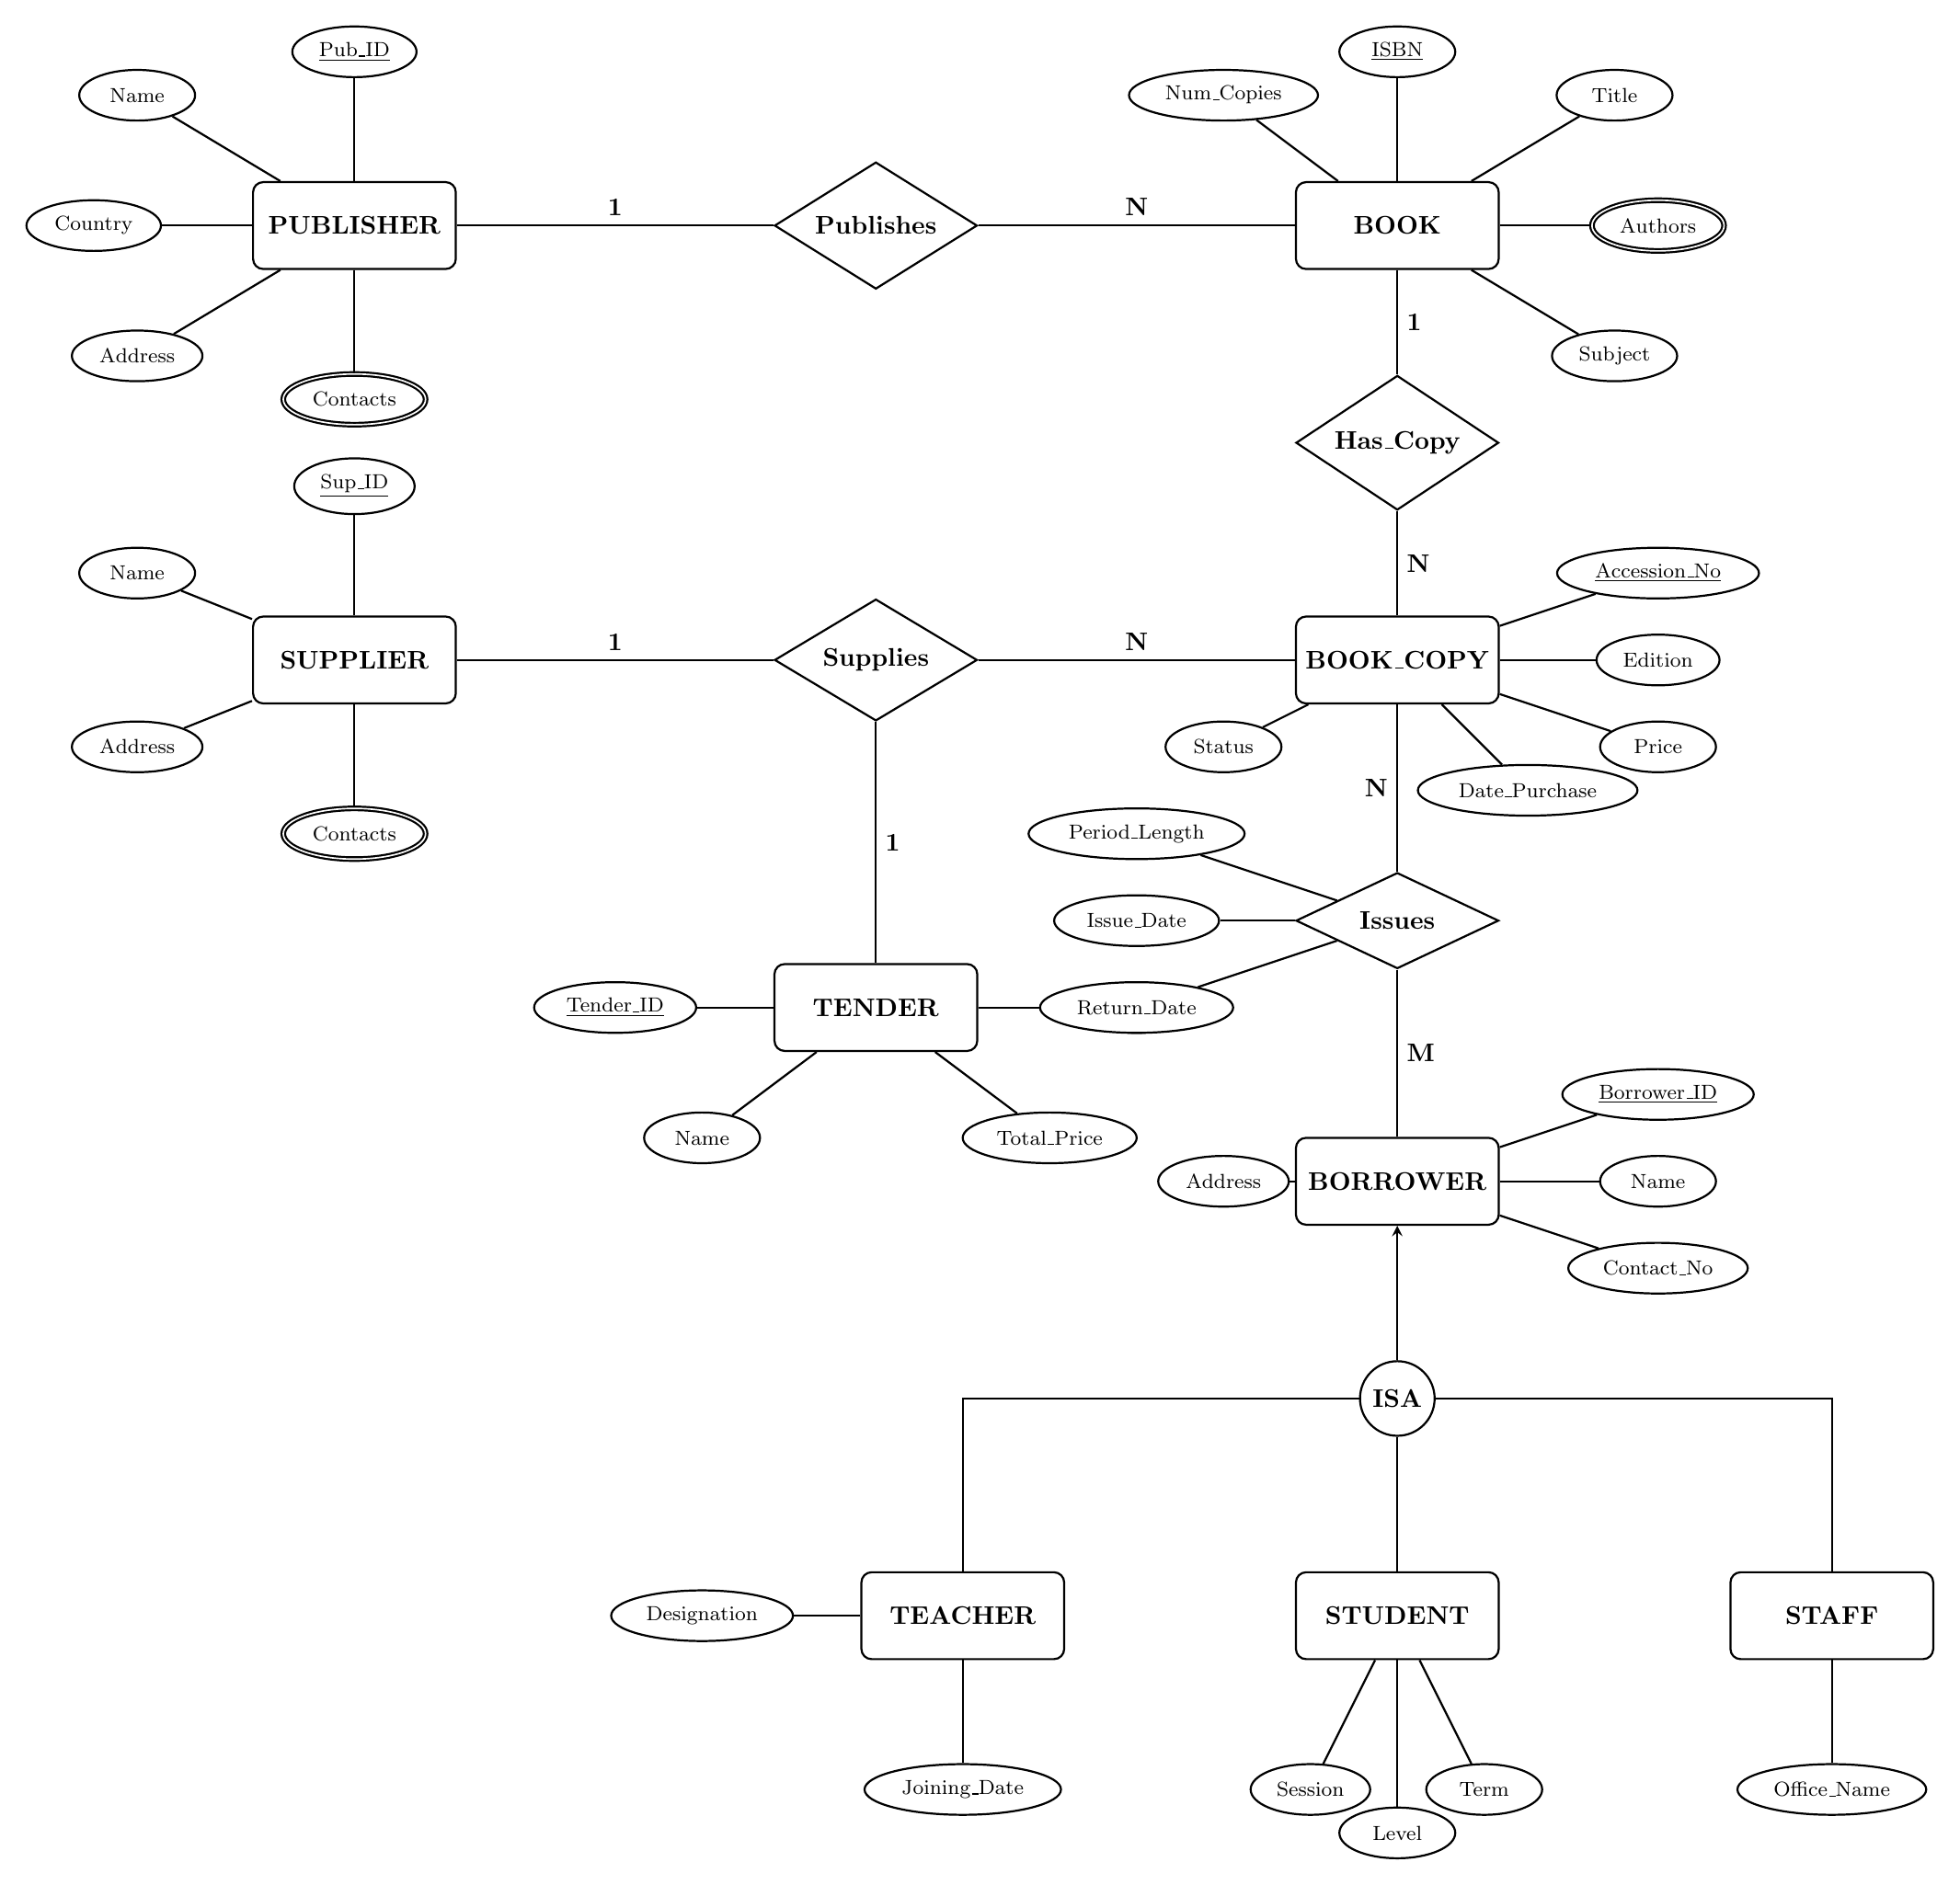
\begin{tikzpicture}[
    thick,x=1.2cm, y=1.2cm, 
    entity/.style={draw, rectangle, rounded corners, minimum width=2.8cm, minimum height=1.2cm, align=center, fill=white, font=\bfseries},
    weakentity/.style={draw, rectangle, double, rounded corners, minimum width=2.8cm, minimum height=1.2cm, align=center, fill=white, font=\bfseries},
    relationship/.style={draw, diamond, aspect=1.5, minimum width=2.8cm, minimum height=1.2cm, align=center, fill=white, font=\bfseries},
    attribute/.style={draw, ellipse, minimum width=1.6cm, minimum height=0.7cm, align=center, fill=white, font=\footnotesize},
    multiattribute/.style={draw, ellipse, double, minimum width=1.6cm, minimum height=0.7cm, align=center, fill=white, font=\footnotesize},
    isa/.style={draw, circle, minimum size=1cm, align=center, fill=white, font=\bfseries}
]

    % ================= ENTITIES =================
    \node[entity] (PUBLISHER) at (-6, 9) {PUBLISHER};
    \node[entity] (BOOK) at (6, 9) {BOOK};
    \node[entity] (BOOK_COPY) at (6, 4) {BOOK\_COPY};
    \node[entity] (SUPPLIER) at (-6, 4) {SUPPLIER};
    \node[entity] (TENDER) at (0, 0) {TENDER};
    \node[entity] (BORROWER) at (6, -2) {BORROWER};
    \node[entity] (TEACHER) at (1, -7) {TEACHER};
    \node[entity] (STUDENT) at (6, -7) {STUDENT};
    \node[entity] (STAFF) at (11, -7) {STAFF};

    % ================= RELATIONSHIPS & ISA =================
    \node[relationship] (PUBLISHES) at (0, 9) {Publishes};
    \node[relationship] (HAS) at (6, 6.5) {Has\_Copy};
    \node[relationship] (SUPPLIES) at (0, 4) {Supplies};
    \node[relationship] (ISSUES) at (6, 1) {Issues};
    \node[isa] (ISA) at (6, -4.5) {ISA};

    % ================= CONNECTIONS =================
    % Publisher - Publishes - Book
    \draw (PUBLISHER) -- (PUBLISHES) node[midway, above, font=\bfseries] {1};
    \draw (PUBLISHES) -- (BOOK) node[midway, above, font=\bfseries] {N};

    % Book - Has - Book Copy
    \draw (BOOK) -- (HAS) node[midway, right, font=\bfseries] {1};
    \draw (HAS) -- (BOOK_COPY) node[midway, right, font=\bfseries] {N};

    % Ternary: Supplier, Tender, Book_Copy -> Supplies
    \draw (SUPPLIER) -- (SUPPLIES) node[midway, above, font=\bfseries] {1};
    \draw (TENDER) -- (SUPPLIES) node[midway, right, font=\bfseries] {1};
    \draw (SUPPLIES) -- (BOOK_COPY) node[midway, above, font=\bfseries] {N};

    % Borrower - Issues - Book Copy
    \draw (BORROWER) -- (ISSUES) node[midway, right, font=\bfseries] {M};
    \draw (ISSUES) -- (BOOK_COPY) node[midway,left, font=\bfseries] {N};

    % ISA Hierarchy
    \draw[->, >=stealth] (ISA) -- (BORROWER);
    \draw (TEACHER) |- (ISA);
    \draw (STUDENT) -- (ISA);
    \draw (STAFF) |- (ISA);

    % ================= ATTRIBUTES =================
    
    % PUBLISHER
    \node[attribute] (p_id) at (-6, 11) {\underline{Pub\_ID}};
    \node[attribute] (p_name) at (-8.5, 10.5) {Name};
    \node[attribute] (p_country) at (-9, 9) {Country};
    \node[attribute] (p_addr) at (-8.5, 7.5) {Address};
    \node[multiattribute] (p_cont) at (-6, 7) {Contacts};
    \draw (PUBLISHER) -- (p_id); \draw (PUBLISHER) -- (p_name); \draw (PUBLISHER) -- (p_country); \draw (PUBLISHER) -- (p_addr); \draw (PUBLISHER) -- (p_cont);

    % BOOK
    \node[attribute] (b_isbn) at (6, 11) {\underline{ISBN}};
    \node[attribute] (b_title) at (8.5, 10.5) {Title};
    \node[multiattribute] (b_auth) at (9, 9) {Authors};
    \node[attribute] (b_subj) at (8.5, 7.5) {Subject};
    \node[attribute] (b_num) at (4, 10.5) {Num\_Copies};
    \draw (BOOK) -- (b_isbn); \draw (BOOK) -- (b_title); \draw (BOOK) -- (b_auth); \draw (BOOK) -- (b_subj); \draw (BOOK) -- (b_num);

    % BOOK COPY
    \node[attribute] (bc_acc) at (9, 5) {\underline{Accession\_No}};
    \node[attribute] (bc_ed) at (9, 4) {Edition};
    \node[attribute] (bc_price) at (9, 3) {Price};
    \node[attribute] (bc_date) at (7.5, 2.5) {Date\_Purchase};
    \node[attribute] (bc_status) at (4, 3) {Status};
    \draw (BOOK_COPY) -- (bc_acc); \draw (BOOK_COPY) -- (bc_ed); \draw (BOOK_COPY) -- (bc_price); \draw (BOOK_COPY) -- (bc_date); \draw (BOOK_COPY) -- (bc_status);

    % SUPPLIER
    \node[attribute] (s_id) at (-6, 6) {\underline{Sup\_ID}};
    \node[attribute] (s_name) at (-8.5, 5) {Name};
    \node[attribute] (s_addr) at (-8.5, 3) {Address};
    \node[multiattribute] (s_cont) at (-6, 2) {Contacts};
    \draw (SUPPLIER) -- (s_id); \draw (SUPPLIER) -- (s_name); \draw (SUPPLIER) -- (s_addr); \draw (SUPPLIER) -- (s_cont);

    % TENDER
    \node[attribute] (t_id) at (-3, 0) {\underline{Tender\_ID}};
    \node[attribute] (t_name) at (-2, -1.5) {Name};
    \node[attribute] (t_price) at (2, -1.5) {Total\_Price};
    \node[attribute] (t_year) at (3, 0) {Year};
    \draw (TENDER) -- (t_id); \draw (TENDER) -- (t_name); \draw (TENDER) -- (t_price); \draw (TENDER) -- (t_year);

    % BORROWER
    \node[attribute] (br_id) at (9, -1) {\underline{Borrower\_ID}};
    \node[attribute] (br_name) at (9, -2) {Name};
    \node[attribute] (br_cont) at (9, -3) {Contact\_No};
    \node[attribute] (br_addr) at (4, -2) {Address};
    \draw (BORROWER) -- (br_id); \draw (BORROWER) -- (br_name); \draw (BORROWER) -- (br_cont); \draw (BORROWER) -- (br_addr);

    % ISSUES ATTRIBUTES
    \node[attribute] (i_date) at (3, 1) {Issue\_Date};
    \node[attribute] (i_ret) at (3, 0) {Return\_Date};
    \node[attribute] (i_len) at (3, 2) {Period\_Length};
    \draw (ISSUES) -- (i_date); \draw (ISSUES) -- (i_ret); \draw (ISSUES) -- (i_len);

    % SUBCLASSES ATTRIBUTES
    \node[attribute] (tc_join) at (1, -9) {Joining\_Date};
    \node[attribute] (tc_desg) at (-2, -7) {Designation};
    \draw (TEACHER) -- (tc_join); \draw (TEACHER) -- (tc_desg);

    \node[attribute] (st_sess) at (5, -9) {Session};
    \node[attribute] (st_lvl) at (6, -9.5) {Level};
    \node[attribute] (st_term) at (7, -9) {Term};
    \draw (STUDENT) -- (st_sess); \draw (STUDENT) -- (st_lvl); \draw (STUDENT) -- (st_term);

    \node[attribute] (sf_off) at (11, -9) {Office\_Name};
    \draw (STAFF) -- (sf_off);

\end{tikzpicture}
}
\end{center}


\vspace{1.5em}
\subsection*{2. Relational Schema (Tables)}

The ER Diagram is mapped to the following normalized relational tables. \textbf{Primary Keys (PK)} are \underline{underlined}, and \textbf{Foreign Keys (FK)} are listed below each relation.

\begin{itemize}[leftmargin=1.5em, itemsep=1em]
    \item \textbf{PUBLISHER} ( \underline{Publisher\_ID}, Name, Country\_of\_Origin, Address )
    \item \textbf{PUBLISHER\_CONTACT} ( \underline{Publisher\_ID}, \underline{Contact\_Number} )
        \begin{itemize}[label={--}, noitemsep, topsep=2pt]
            \item \textit{FK: Publisher\_ID references PUBLISHER(Publisher\_ID)}
        \end{itemize}

    \item \textbf{BOOK} ( \underline{ISBN}, Title, Subject, Number\_of\_Copies, Publisher\_ID )
        \begin{itemize}[label={--}, noitemsep, topsep=2pt]
            \item \textit{FK: Publisher\_ID references PUBLISHER(Publisher\_ID)}
        \end{itemize}
    \item \textbf{BOOK\_AUTHOR} ( \underline{ISBN}, \underline{Author\_Name} )
        \begin{itemize}[label={--}, noitemsep, topsep=2pt]
            \item \textit{FK: ISBN references BOOK(ISBN)}
        \end{itemize}

    \item \textbf{SUPPLIER} ( \underline{Supplier\_ID}, Name, Address )
    \item \textbf{SUPPLIER\_CONTACT} ( \underline{Supplier\_ID}, \underline{Contact\_Number} )
        \begin{itemize}[label={--}, noitemsep, topsep=2pt]
            \item \textit{FK: Supplier\_ID references SUPPLIER(Supplier\_ID)}
        \end{itemize}

    \item \textbf{TENDER} ( \underline{Tender\_ID}, Name, Total\_Price, Year )

    \item \textbf{BOOK\_COPY} ( \underline{Accession\_Number}, Edition, Price, Date\_of\_Purchase, Status, ISBN, Supplier\_ID, Tender\_ID )
        \begin{itemize}[label={--}, noitemsep, topsep=2pt]
            \item \textit{FK: ISBN references BOOK(ISBN)}
            \item \textit{FK: Supplier\_ID references SUPPLIER(Supplier\_ID)}
            \item \textit{FK: Tender\_ID references TENDER(Tender\_ID)}
        \end{itemize}
        
    \item \textbf{BORROWER} ( \underline{Borrower\_ID}, Name, Contact\_Number, Address )
    
    \item \textbf{TEACHER} ( \underline{Borrower\_ID}, Joining\_Date, Designation )
        \begin{itemize}[label={--}, noitemsep, topsep=2pt]
            \item \textit{FK: Borrower\_ID references BORROWER(Borrower\_ID)}
        \end{itemize}
        
    \item \textbf{STUDENT} ( \underline{Borrower\_ID}, Session, Level, Term )
        \begin{itemize}[label={--}, noitemsep, topsep=2pt]
            \item \textit{FK: Borrower\_ID references BORROWER(Borrower\_ID)}
        \end{itemize}
        
    \item \textbf{STAFF} ( \underline{Borrower\_ID}, Office\_Name )
        \begin{itemize}[label={--}, noitemsep, topsep=2pt]
            \item \textit{FK: Borrower\_ID references BORROWER(Borrower\_ID)}
        \end{itemize}

    \item \textbf{ISSUE} ( \underline{Borrower\_ID}, \underline{Accession\_Number}, \underline{Issue\_Date}, Length\_of\_Period, Return\_Date )
        \begin{itemize}[label={--}, noitemsep, topsep=2pt]
            \item \textit{FK: Borrower\_ID references BORROWER(Borrower\_ID)}
            \item \textit{FK: Accession\_Number references BOOK\_COPY(Accession\_Number)}
        \end{itemize}
\end{itemize}

\end{tcolorbox}

\item East West Property Development is a construction company of Bashundhara Group with over 1000 employees. A customer can hire the company for more than one project, and employees sometimes work on more than one project at a time. Equipment is assigned to only one project. Draw an E-R diagram for this company indicating cardinality.
\mk{7} \yr{CSE 303 | L-3/T-1 | 2015--16}

\begin{tcolorbox}[enhanced,breakable,ansbox,colback=cA!4,colframe=cA,boxrule=0.8pt,arc=5pt,title={\textbf{Answer}},fonttitle=\bfseries\color{white},colbacktitle=cA]

\subsection*{1. Entity and Relationship Analysis}

Based on the scenario provided for East West Property Development, we can identify the following entities, relationships, and their respective cardinalities. Since specific attributes were not detailed in the prompt, standard identifier (primary key) and descriptive attributes have been assumed for completeness.

\begin{itemize}[leftmargin=2em, itemsep=0.5em]
    \item \textbf{Entities:}
    \begin{itemize}[label={--}, itemsep=1pt]
        \item \textbf{CUSTOMER}: Represents the clients who hire the company.
        \item \textbf{PROJECT}: Represents the construction projects undertaken by the company.
        \item \textbf{EMPLOYEE}: Represents the workforce of the company.
        \item \textbf{EQUIPMENT}: Represents the machinery/tools used in construction.
    \end{itemize}

    \item \textbf{Relationships and Cardinalities:}
    \begin{itemize}[label={--}, itemsep=1pt]
        \item \textbf{Hires (CUSTOMER and PROJECT):} A \textbf{One-to-Many (1:N)} relationship. A customer can hire the company for more than one project (N), but a specific project is typically commissioned by a single customer (1).
        \item \textbf{Works\_On (EMPLOYEE and PROJECT):} A \textbf{Many-to-Many (M:N)} relationship. Employees can work on more than one project at a time (N), and a construction project naturally requires multiple employees (M).
        \item \textbf{Assigned\_To (EQUIPMENT and PROJECT):} A \textbf{Many-to-One (N:1)} relationship. Equipment is assigned to only one project at a time (1), but a single project will require multiple pieces of equipment (N).
    \end{itemize}
\end{itemize}

\vspace{1em}
\subsection*{2. Entity-Relationship (ER) Diagram}

The following ER diagram uses standard Chen's notation to visualize the organizational data requirements.

\vspace{1.5em}
\begin{center}
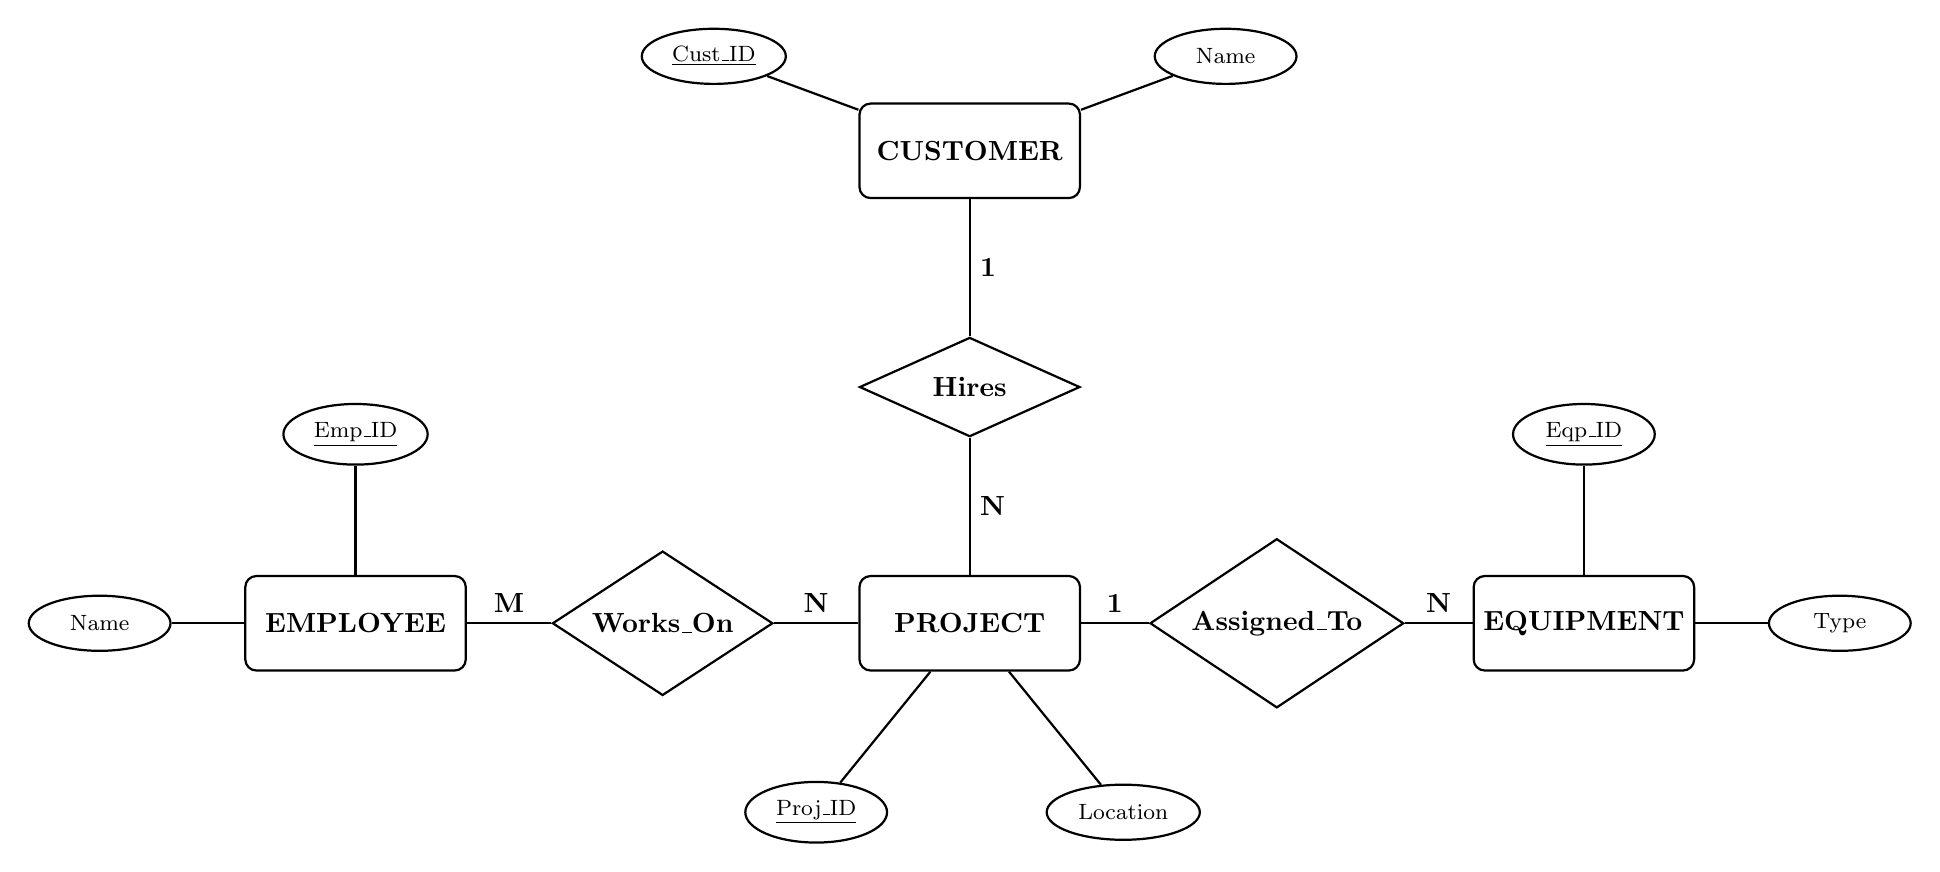
\begin{tikzpicture}[
    thick,x=1.3cm, y=1.2cm,
    entity/.style={draw, rectangle, rounded corners, minimum width=2.8cm, minimum height=1.2cm, align=center, fill=white, font=\bfseries},
    relationship/.style={draw, diamond, aspect=1.5, minimum width=2.8cm, minimum height=1.2cm, align=center, fill=white, font=\bfseries},
    attribute/.style={draw, ellipse, minimum width=1.8cm, minimum height=0.7cm, align=center, fill=white, font=\footnotesize}
]

    % ================= ENTITIES =================
    \node[entity] (PROJ) at (0, 0) {PROJECT};
    \node[entity] (CUST) at (0, 5) {CUSTOMER};
    \node[entity] (EMP)  at (-6, 0) {EMPLOYEE};
    \node[entity] (EQP)  at (6, 0) {EQUIPMENT};

    % ================= RELATIONSHIPS =================
    \node[relationship] (HIRES) at (0, 2.5) {Hires};
    \node[relationship] (WORKS) at (-3, 0) {Works\_On};
    \node[relationship] (ASSGN) at (3, 0) {Assigned\_To};

    % ================= CONNECTIONS WITH MULTIPLICITIES =================
    % Customer - Hires - Project (1:N)
    \draw (CUST) -- (HIRES) node[midway, right, font=\bfseries] {1};
    \draw (HIRES) -- (PROJ) node[midway, right, font=\bfseries] {N};

    % Employee - Works_On - Project (M:N)
    \draw (EMP) -- (WORKS) node[midway, above, font=\bfseries] {M};
    \draw (WORKS) -- (PROJ) node[midway, above, font=\bfseries] {N};

    % Equipment - Assigned_To - Project (N:1)
    \draw (EQP) -- (ASSGN) node[midway, above, font=\bfseries] {N}; 
    \draw (ASSGN) -- (PROJ) node[midway, above, font=\bfseries] {1}; 

    % ================= ATTRIBUTES (Assumed for Completeness) =================
    
    % CUSTOMER Attributes
    \node[attribute] (c_id) at (-2.5, 6) {\underline{Cust\_ID}};
    \node[attribute] (c_name) at (2.5, 6) {Name};
    \draw (CUST) -- (c_id);
    \draw (CUST) -- (c_name);

    % EMPLOYEE Attributes
    \node[attribute] (e_id) at (-6, 2) {\underline{Emp\_ID}};
    \node[attribute] (e_name) at (-8.5, 0) {Name};
    \draw (EMP) -- (e_id);
    \draw (EMP) -- (e_name);

    % PROJECT Attributes
    \node[attribute] (p_id) at (-1.5, -2) {\underline{Proj\_ID}};
    \node[attribute] (p_name) at (1.5, -2) {Location};
    \draw (PROJ) -- (p_id);
    \draw (PROJ) -- (p_name);

    % EQUIPMENT Attributes
    \node[attribute] (eq_id) at (6, 2) {\underline{Eqp\_ID}};
    \node[attribute] (eq_name) at (8.5, 0) {Type};
    \draw (EQP) -- (eq_id);
    \draw (EQP) -- (eq_name);

\end{tikzpicture}
\end{center}

\end{tcolorbox}

\item A university has a large number of courses. Each course may have one or more different courses as prerequisites, or may have no prerequisites. Similarly, a particular course may be a prerequisite of any number of courses or may not be a prerequisite of any other course. Sketch an E-R diagram that includes \textbf{COURSE} as the single entity, including cardinality. Each course has a course number and title. Convert the E-R diagram into a relational schema.
\mk{7} \yr{CSE 303 | L-3/T-1 | 2015--16}

\begin{tcolorbox}[enhanced,breakable,ansbox,colback=cA!4,colframe=cA,boxrule=0.8pt,arc=5pt,title={\textbf{Answer}},fonttitle=\bfseries\color{white},colbacktitle=cA]

\subsection*{1. Entity-Relationship (ER) Diagram}

The scenario describes a \textbf{Unary (Recursive) Relationship} on a single entity \textbf{COURSE}. Since a course can have many prerequisites, and a course can be a prerequisite for many other courses, the relationship between \textbf{COURSE} and itself is \textbf{Many-to-Many (M:N)}. 

To clarify the recursive relationship, \textit{roles} (``Main Course'' and ``Prerequisite'') are indicated on the edges connecting the entity to the relationship diamond.

\vspace{1.5em}
\begin{center}
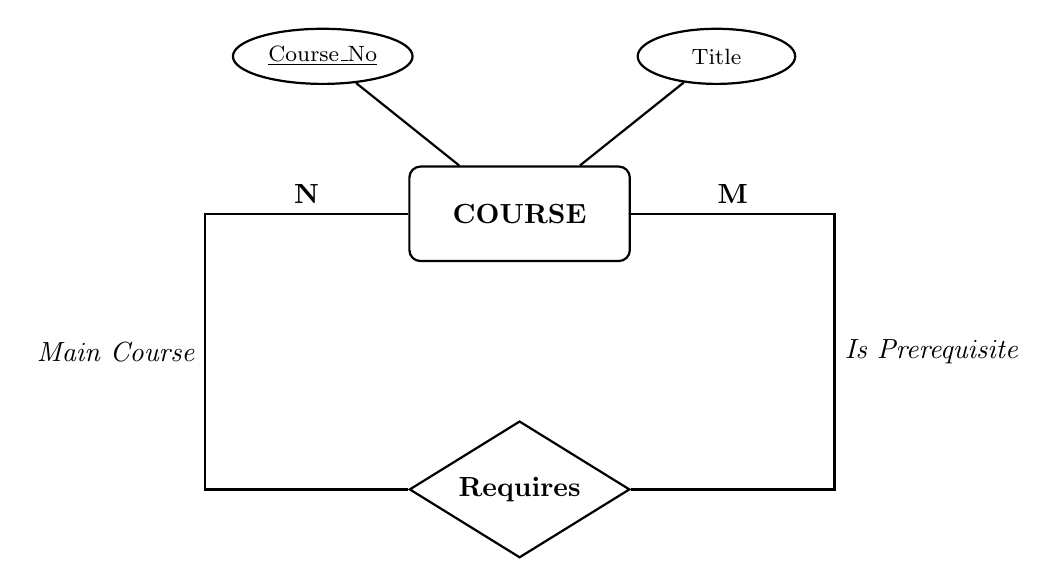
\begin{tikzpicture}[
    thick,
    entity/.style={draw, rectangle, rounded corners, minimum width=2.8cm, minimum height=1.2cm, align=center, fill=white, font=\bfseries},
    relationship/.style={draw, diamond, aspect=1.5, minimum width=2.8cm, minimum height=1.2cm, align=center, fill=white, font=\bfseries},
    attribute/.style={draw, ellipse, minimum width=2cm, minimum height=0.7cm, align=center, fill=white, font=\footnotesize}
]

    % ================= ENTITY AND RELATIONSHIP =================
    \node[entity] (COURSE) at (0, 0) {COURSE};
    \node[relationship] (REQ) at (0, -3.5) {Requires};

    % ================= ATTRIBUTES =================
    \node[attribute] (CNO) at (-2.5, 2) {\underline{Course\_No}};
    \node[attribute] (TITLE) at (2.5, 2) {Title};

    \draw (COURSE) -- (CNO);
    \draw (COURSE) -- (TITLE);

    % ================= RECURSIVE CONNECTIONS =================
    % Left side routing: Main Course role
    \draw (COURSE.west) 
        -- (-4, 0) node[midway, above, font=\bfseries] {N} 
        -- (-4, -3.5) node[midway, left, font=\itshape] {Main Course} 
        -- (REQ.west);
        
    % Right side routing: Prerequisite role
    \draw (COURSE.east) 
        -- (4, 0) node[midway, above, font=\bfseries] {M} 
        -- (4, -3.5) node[midway, right, font=\itshape] {Is Prerequisite} 
        -- (REQ.east);

\end{tikzpicture}
\end{center}
\vspace{1em}

\subsection*{2. Relational Schema}

To convert an $M:N$ recursive relationship into a relational schema, we must create two tables: one for the entity itself, and a junction (associative) table to represent the $M:N$ relationship. The primary keys (PK) are \underline{underlined}.

\vspace{1em}

\begin{itemize}[leftmargin=2em, itemsep=1em]
    \item \textbf{COURSE} ( \underline{Course\_No}, Title )
    \item \textbf{PREREQUISITE} ( \underline{Course\_No}, \underline{Prereq\_No} )
\end{itemize}

\vspace{1em}

\subsubsection*{Foreign Key Constraints and Dependencies}

\begin{center}
\renewcommand{\arraystretch}{1.4}
\begin{tabular}{@{} l l l @{}}
\toprule
\textbf{Relation} & \textbf{Foreign Key Attribute(s)} & \textbf{References} \\
\midrule
\textbf{COURSE}       & None & N/A \\
\textbf{PREREQUISITE} & \textbf{Course\_No} & \textbf{COURSE} (Course\_No) \\
\textbf{PREREQUISITE} & \textbf{Prereq\_No} & \textbf{COURSE} (Course\_No) \\
\bottomrule
\end{tabular}
\end{center}

\vspace{0.5em}
\textbf{Note:} In the \textbf{PREREQUISITE} table, both \texttt{Course\_No} and \texttt{Prereq\_No} act together as a composite Primary Key to uniquely identify a prerequisite pairing. Simultaneously, each attribute independently acts as a Foreign Key referencing the \textbf{COURSE} table.

\end{tcolorbox}

\item Consider the following information about a university database. Professors have an SSN, a name, an age, a rank, and a research speciality. Projects have a project number, a sponsor name (e.g., NSF), a starting date, an ending date, and a budget. Graduate students have an SSN, a name, an age, and a degree program (e.g., M.S.\ or Ph.D). Each project is managed by one professor (the principal investigator). Each project is worked on by one or more professors (co-investigators). Professors can manage and/or work on multiple projects. Each project is worked on by one or more graduate students (research assistants). When graduate students work on a project, a professor must supervise their work. Graduate students can work on multiple projects, having a (potentially different) supervisor for each. Departments have a department number, name, and main office. A professor (chairman) runs each department. Professors work in one or more departments with a time percentage per department. Graduate students have one major department. Each graduate student has a more senior graduate student (student advisor) who advises on course selection.
Draw an Entity-Relationship (ER) diagram to represent the data requirements described above.
\mk{18} \yr{CSE 303 | L-3/T-1 | 2014--15}

\begin{tcolorbox}[enhanced,breakable,ansbox,colback=cA!4,colframe=cA,boxrule=0.8pt,arc=5pt,title={\textbf{Answer}},fonttitle=\bfseries\color{white},colbacktitle=cA]

\subsection*{Entity-Relationship (ER) Diagram}

The following ER diagram captures all the specified data requirements, including the ternary relationship for student project supervision, recursive relationship for student advising, and partial/total participation constraints.

\vspace{1.5em}
\begin{center}
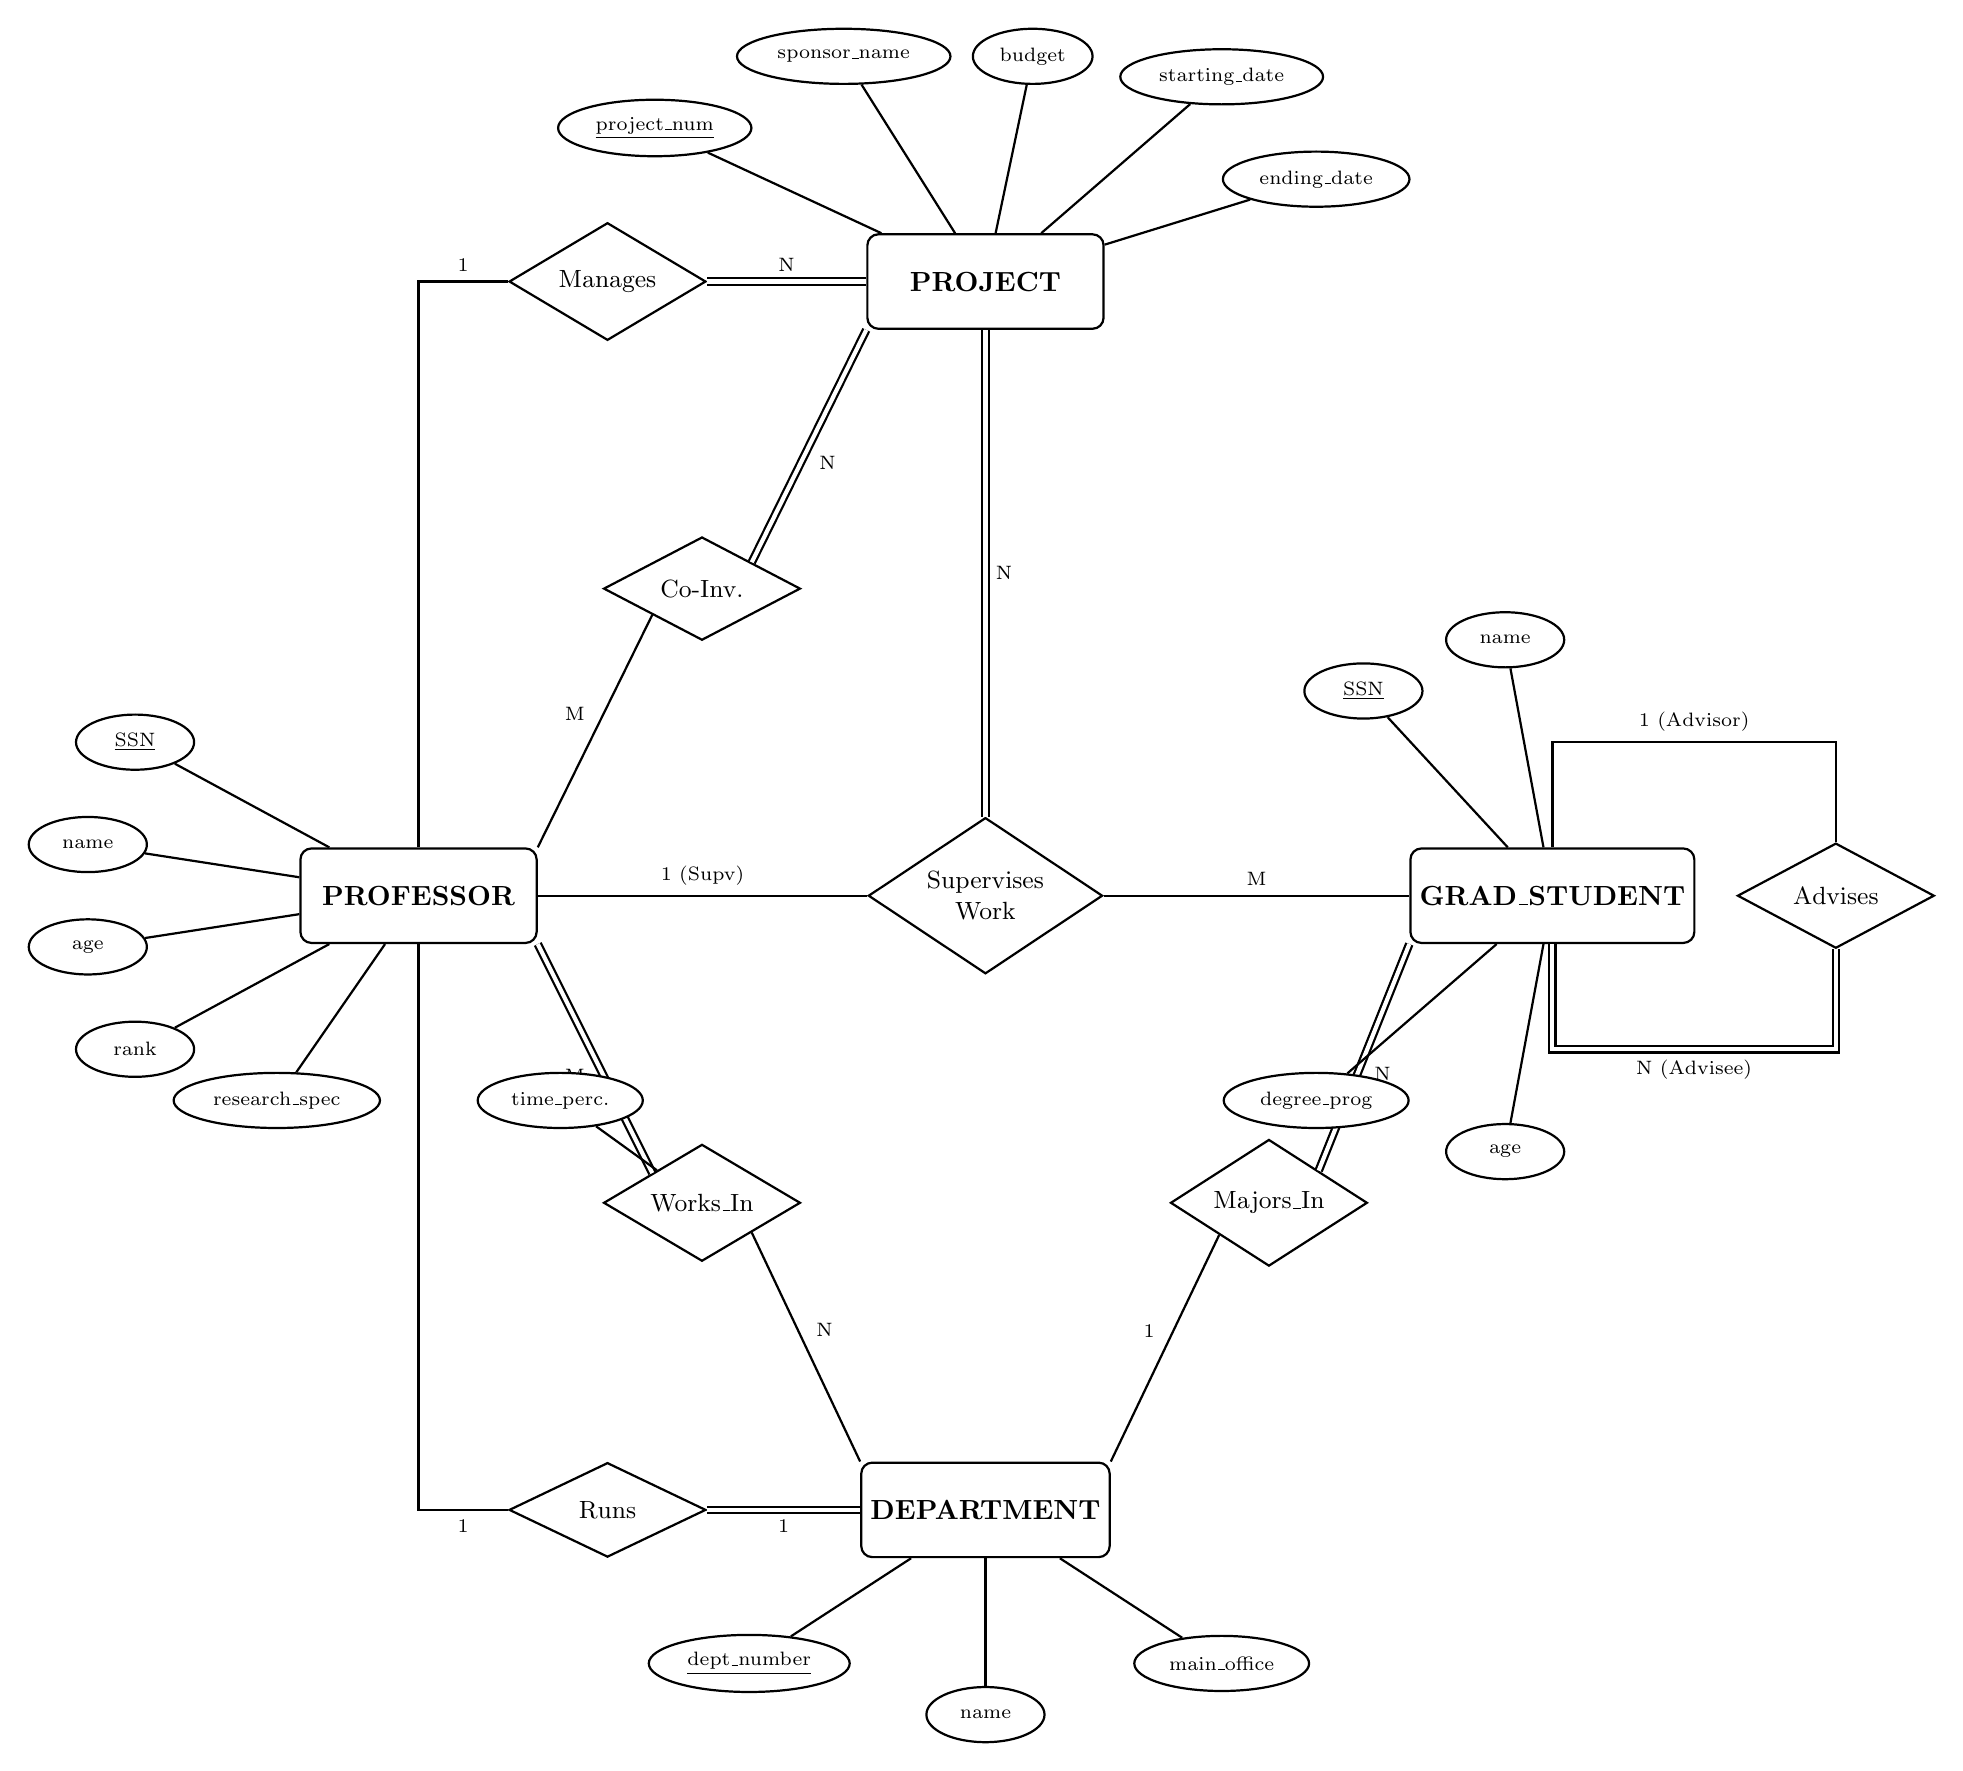
\begin{tikzpicture}[
    x=1.2cm, y=1.3cm,
    entity/.style={draw, rectangle, rounded corners, minimum width=3cm, minimum height=1.2cm, align=center, fill=white, thick, font=\bfseries},
    relationship/.style={draw, diamond, aspect=1.5, minimum width=2.5cm, minimum height=1.2cm, align=center, fill=white, thick},
    attribute/.style={draw, ellipse, minimum width=1.5cm, minimum height=0.7cm, align=center, fill=white, font=\scriptsize, thick},
    every node/.style={font=\small}
]

    % ===============================
    % 1. ENTITIES
    % ===============================
    \node[entity] (prof) at (-6, 0) {PROFESSOR};
    \node[entity] (grad) at (6, 0) {GRAD\_STUDENT};
    \node[entity] (proj) at (0, 6) {PROJECT};
    \node[entity] (dept) at (0, -6) {DEPARTMENT};

    % ===============================
    % 2. RELATIONSHIPS & CONNECTIONS
    % ===============================

    % A. Manages (Prof -> Proj) : 1 to N, Proj Total
    \node[relationship] (manages) at (-4, 6) {Manages};
    \draw[thick] (prof.north) -- (-6, 6) -- (manages.west) node[pos=0.5, above, font=\scriptsize] {1};
    \draw[thick, double, double distance=1.5pt] (manages.east) -- (proj.west) node[midway, above, font=\scriptsize] {N};

    % B. Runs (Prof -> Dept) : 1 to 1, Dept Total
    \node[relationship] (runs) at (-4, -6) {Runs};
    \draw[thick] (prof.south) -- (-6, -6) -- (runs.west) node[pos=0.5, below, font=\scriptsize] {1};
    \draw[thick, double, double distance=1.5pt] (runs.east) -- (dept.west) node[midway, below, font=\scriptsize] {1};

    % C. Co-Investigates (Prof -> Proj) : M to N, Proj Total
    \node[relationship] (coinv) at (-3, 3) {Co-Inv.};
    \draw[thick] (prof.north east) -- (coinv.south west) node[midway, above left, font=\scriptsize] {M};
    \draw[thick, double, double distance=1.5pt] (coinv.north east) -- (proj.south west) node[midway, below right, font=\scriptsize] {N};

    % D. Works_In (Prof -> Dept) : M to N, Prof Total
    \node[relationship] (worksin) at (-3, -3) {Works\_In};
    \draw[thick, double, double distance=1.5pt] (prof.south east) -- (worksin.north west) node[midway, below left, font=\scriptsize] {M};
    \draw[thick] (worksin.south east) -- (dept.north west) node[midway, above right, font=\scriptsize] {N};
    
    % Attribute of Works_In
    \node[attribute] (time) at (-4.5, -2) {time\_perc.};
    \draw[thick] (worksin) -- (time);

    % E. Majors_In (Grad -> Dept) : N to 1, Grad Total
    \node[relationship] (majors) at (3, -3) {Majors\_In};
    \draw[thick, double, double distance=1.5pt] (grad.south west) -- (majors.north east) node[midway, below right, font=\scriptsize] {N};
    \draw[thick] (majors.south west) -- (dept.north east) node[midway, above left, font=\scriptsize] {1};

    % F. Supervises_Work (Ternary: Prof, Grad, Proj)
    \node[relationship, align=center] (supervises) at (0, 0) {Supervises\\Work};
    \draw[thick] (supervises.west) -- (prof.east) node[midway, above, font=\scriptsize] {1 (Supv)};
    \draw[thick] (supervises.east) -- (grad.west) node[midway, above, font=\scriptsize] {M};
    \draw[thick, double, double distance=1.5pt] (supervises.north) -- (proj.south) node[midway, right, font=\scriptsize] {N};

    % G. Advises (Grad -> Grad Recursive) : 1 to N, Advisee Total
    \node[relationship] (advises) at (9, 0) {Advises};
    \draw[thick] (grad.north) -- (6, 1.5) -- (9, 1.5) node[midway, above, font=\scriptsize] {1 (Advisor)} -- (advises.north);
    \draw[thick, double, double distance=1.5pt] (grad.south) -- (6, -1.5) -- (9, -1.5) node[midway, below, font=\scriptsize] {N (Advisee)} -- (advises.south);


    % ===============================
    % 3. ATTRIBUTES
    % ===============================
    
    % PROFESSOR Attributes
    \node[attribute] (pssn) at (-9, 1.5) {\underline{SSN}};
    \node[attribute] (pname) at (-9.5, 0.5) {name};
    \node[attribute] (page) at (-9.5, -0.5) {age};
    \node[attribute] (prank) at (-9, -1.5) {rank};
    \node[attribute] (pspec) at (-7.5, -2) {research\_spec};
    
    \draw[thick] (prof) -- (pssn);
    \draw[thick] (prof) -- (pname);
    \draw[thick] (prof) -- (page);
    \draw[thick] (prof) -- (prank);
    \draw[thick] (prof) -- (pspec);

    % PROJECT Attributes
    \node[attribute] (pjnum) at (-3.5, 7.5) {\underline{project\_num}};
    \node[attribute] (pjspon) at (-1.5, 8.2) {sponsor\_name};
    \node[attribute] (pjbud) at (0.5, 8.2) {budget};
    \node[attribute] (pjstart) at (2.5, 8) {starting\_date};
    \node[attribute] (pjend) at (3.5, 7) {ending\_date};
    
    \draw[thick] (proj) -- (pjnum);
    \draw[thick] (proj) -- (pjspon);
    \draw[thick] (proj) -- (pjbud);
    \draw[thick] (proj) -- (pjstart);
    \draw[thick] (proj) -- (pjend);

    % DEPARTMENT Attributes
    \node[attribute] (dnum) at (-2.5, -7.5) {\underline{dept\_number}};
    \node[attribute] (dname) at (0, -8) {name};
    \node[attribute] (doff) at (2.5, -7.5) {main\_office};
    
    \draw[thick] (dept) -- (dnum);
    \draw[thick] (dept) -- (dname);
    \draw[thick] (dept) -- (doff);

    % GRAD_STUDENT Attributes
    \node[attribute] (gssn) at (4, 2) {\underline{SSN}};
    \node[attribute] (gname) at (5.5, 2.5) {name};
    \node[attribute] (gage) at (5.5, -2.5) {age};
    \node[attribute] (gdeg) at (3.5, -2) {degree\_prog};
    
    \draw[thick] (grad) -- (gssn);
    \draw[thick] (grad) -- (gname);
    \draw[thick] (grad) -- (gage);
    \draw[thick] (grad) -- (gdeg);

\end{tikzpicture}
\end{center}

\vspace{1em}
\subsection*{Design Notes \& Assumptions}
\begin{itemize}
    \item \textbf{Ternary Relationship (\texttt{Supervises\_Work}):} Associates \texttt{PROFESSOR}, \texttt{GRAD\_STUDENT}, and \texttt{PROJECT}. A student working on a specific project must be supervised by one professor.
    \item \textbf{Total Participation (Double Lines):} 
    \begin{itemize}
        \item \texttt{PROJECT} must have a PI (\texttt{Manages}) and co-investigators (\texttt{Co-Inv.}).
        \item \texttt{DEPARTMENT} must be run by a chairman (\texttt{Runs}).
        \item \texttt{PROFESSOR} must work in at least one department (\texttt{Works\_In}).
        \item \texttt{GRAD\_STUDENT} must have a major department (\texttt{Majors\_In}) and an advisor (\texttt{Advises}).
    \end{itemize}
    \item \textbf{Recursive Relationship:} The \texttt{Advises} relationship maps senior graduate students (1) to their respective junior advisees (N).
    \item \textbf{Relationship Attributes:} The `time percentage` is modeled as a descriptive attribute of the \texttt{Works\_In} M:N relationship, as it characterizes the specific assignment between a professor and a department.
\end{itemize}

\end{tcolorbox}

%% Q5
\item A library keeps records of current loans of books to borrowers. Each borrower is identified by a borrower number and each copy of a book by an accession number (the library may have more than one copy of any given book). The name and address of each borrower is held so that overdue loan reminders can be sent. Information held about books includes the title, author's name(s), publisher's name, publication date, ISBN, purchase price, classification (reference or fiction), and number of pages. A given book may be written by a number of authors; the library regards a book as only being published by a single publisher. The library assigns its own unique in-house codes for authors and publishers.

A book may cover a number of different subjects, and borrowers can use an online catalogue to select texts by subject as well as title and author. There is a restriction on the number of books a borrower may have on loan at any time and the loan period --- these limits depend on the borrower's classification (junior, adult, or organisation). When a book is borrowed, the return date is automatically recorded. Other borrowers may reserve books out on loan. A special borrower's status flag is maintained --- borrowers who hold overdue books or have reached their loan limit are flagged to prevent further borrowings.

Draw an Entity-Relationship (ER) diagram to represent the Library data requirements described above.
\mk{18} \yr{CSE 303 | L-3/T-1 | 2013--14}

\begin{tcolorbox}[enhanced,breakable,ansbox,colback=cA!4,colframe=cA,boxrule=0.8pt,arc=5pt,title={\textbf{Answer}},fonttitle=\bfseries\color{white},colbacktitle=cA]

\subsection*{1. Entity-Relationship (ER) Diagram Analysis}

Based on the library data requirements provided, the following elements are identified to form the ER diagram:

\begin{itemize}[leftmargin=2em, itemsep=0.5em]
    \item \textbf{Entities and Primary Keys:}
    \begin{itemize}[label={--}, itemsep=2pt]
        \item \textbf{BOOK}: Identified by \underline{ISBN}. Attributes include Title, Pub\_Date, Price, Book\_Class, and Num\_Pages.
        \item \textbf{AUTHOR}: Identified by \underline{Author\_Code}. Attributes include Name.
        \item \textbf{PUBLISHER}: Identified by \underline{Pub\_Code}. Attributes include Name.
        \item \textbf{SUBJECT}: Identified by \underline{Subj\_Name}. 
        \item \textbf{BOOK\_COPY}: Identified by \underline{Accession\_No}. A strong entity as accession numbers are globally unique in a library system.
        \item \textbf{BORROWER}: Identified by \underline{Borrower\_No}. Attributes include Name, Address, and Status\_Flag.
        \item \textbf{BORROWER\_CLASS}: Identified by \underline{Class\_Name} (e.g., junior, adult, organisation). Attributes include Loan\_Limit and Loan\_Period. Extracted into a separate entity to enforce the business rule that limits depend strictly on classification.
    \end{itemize}

    \item \textbf{Relationships and Cardinalities:}
    \begin{itemize}[label={--}, itemsep=2pt]
        \item \textbf{Published\_By}: N:1 between BOOK and PUBLISHER.
        \item \textbf{Written\_By}: M:N between BOOK and AUTHOR.
        \item \textbf{Covers}: M:N between BOOK and SUBJECT.
        \item \textbf{Has\_Copy}: 1:N between BOOK and BOOK\_COPY. BOOK\_COPY has total participation.
        \item \textbf{Borrows}: M:N between BORROWER and BOOK\_COPY. Incorporates the automatically recorded attribute \textit{Return\_Date}.
        \item \textbf{Reserves}: M:N between BORROWER and BOOK.
        \item \textbf{Has\_Type}: N:1 between BORROWER and BORROWER\_CLASS.
    \end{itemize}
\end{itemize}

\vspace{1em}
\subsection*{2. Entity-Relationship Diagram}
\vspace{1em}


\begin{center}
\resizebox{\textwidth}{!}{
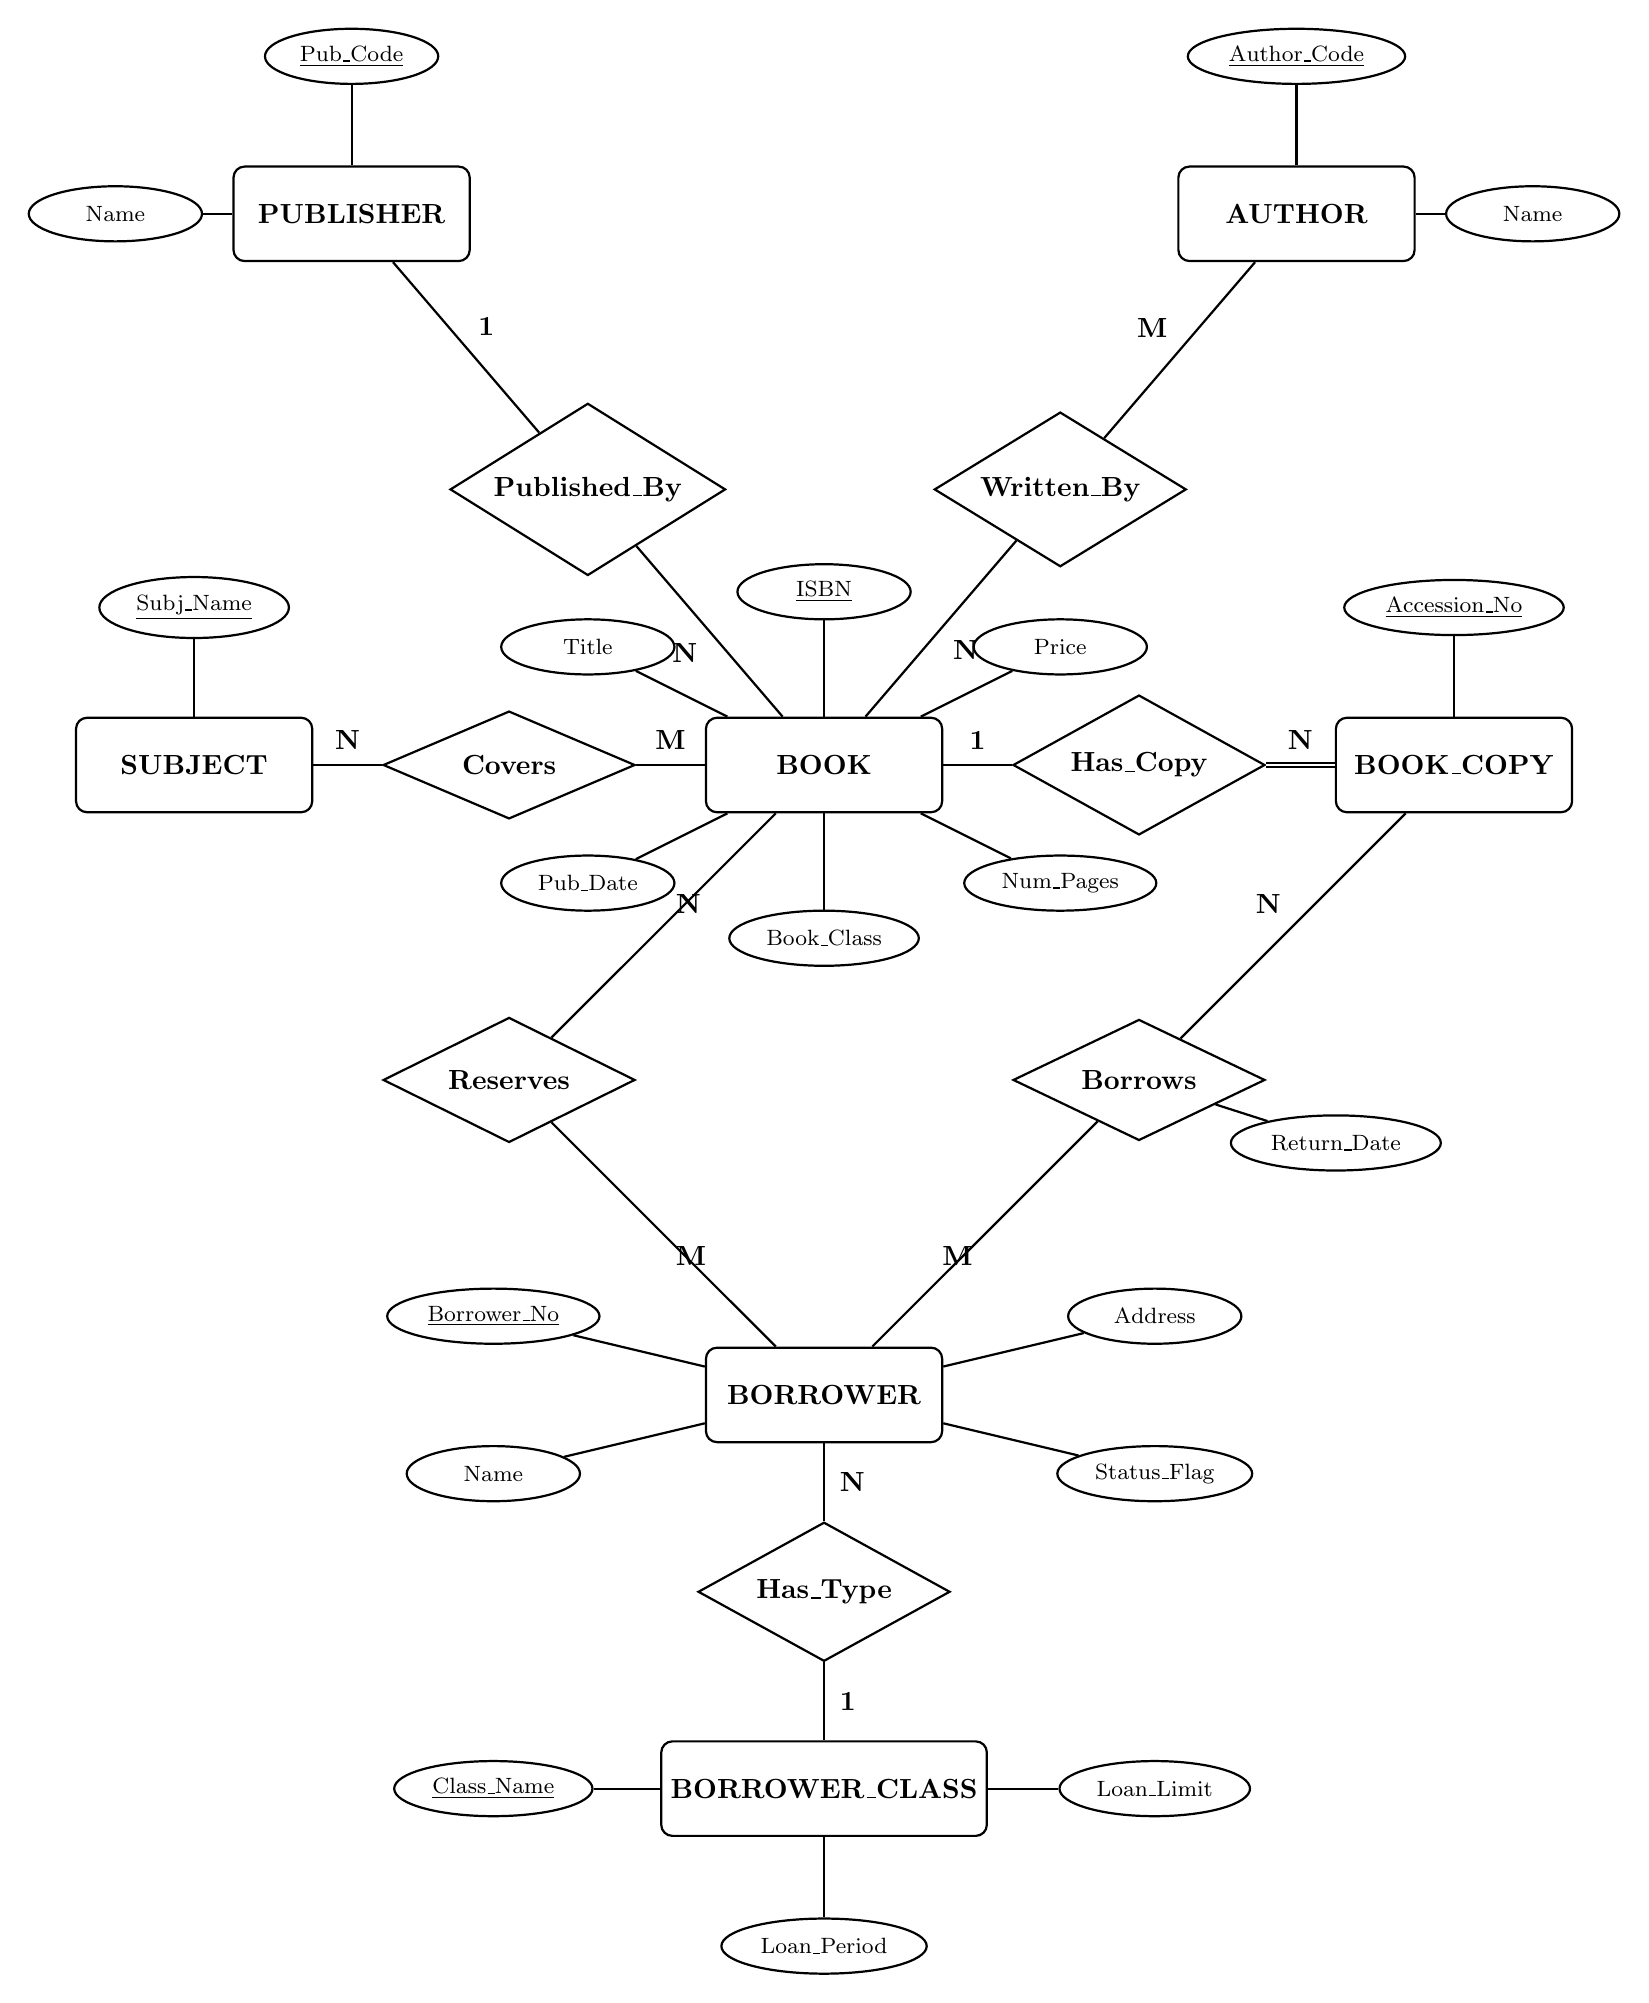
\begin{tikzpicture}[
    thick,
    entity/.style={draw, rectangle, rounded corners, minimum width=3cm, minimum height=1.2cm, align=center, fill=white, font=\bfseries},
    relationship/.style={draw, diamond, aspect=1.6, minimum width=3.2cm, minimum height=1.2cm, align=center, fill=white, font=\bfseries},
    attribute/.style={draw, ellipse, minimum width=2.2cm, minimum height=0.7cm, align=center, fill=white, font=\footnotesize}
]

    % ================= ENTITIES =================
    \node[entity] (PUBLISHER) at (-6, 7) {PUBLISHER};
    \node[entity] (AUTHOR) at (6, 7) {AUTHOR};
    \node[entity] (BOOK) at (0, 0) {BOOK};
    \node[entity] (SUBJECT) at (-8, 0) {SUBJECT};
    \node[entity] (BOOKCOPY) at (8, 0) {BOOK\_COPY};
    \node[entity] (BORROWER) at (0, -8) {BORROWER};
    \node[entity] (BORRCLASS) at (0, -13) {BORROWER\_CLASS};

    % ================= RELATIONSHIPS =================
    \node[relationship] (PUB_REL) at (-3, 3.5) {Published\_By};
    \node[relationship] (AUTH_REL) at (3, 3.5) {Written\_By};
    \node[relationship] (SUBJ_REL) at (-4, 0) {Covers};
    \node[relationship] (COPY_REL) at (4, 0) {Has\_Copy};
    \node[relationship] (RES_REL) at (-4, -4) {Reserves};
    \node[relationship] (LOAN_REL) at (4, -4) {Borrows};
    \node[relationship] (BELONGS) at (0, -10.5) {Has\_Type};

    % ================= CONNECTIONS WITH MULTIPLICITIES =================
    
    % PUBLISHER - BOOK
    \draw (PUBLISHER) -- (PUB_REL) node[midway, above right=1pt, font=\bfseries] {1};
    \draw (PUB_REL) -- (BOOK) node[midway, below left=1pt, font=\bfseries] {N};

    % AUTHOR - BOOK
    \draw (AUTHOR) -- (AUTH_REL) node[midway, above left=1pt, font=\bfseries] {M};
    \draw (AUTH_REL) -- (BOOK) node[midway, below right=1pt, font=\bfseries] {N};

    % SUBJECT - BOOK
    \draw (SUBJECT) -- (SUBJ_REL) node[midway, above=2pt, font=\bfseries] {N};
    \draw (SUBJ_REL) -- (BOOK) node[midway, above=2pt, font=\bfseries] {M};

    % BOOK - BOOK_COPY (Total Participation for BOOK_COPY)
    \draw (BOOK) -- (COPY_REL) node[midway, above=2pt, font=\bfseries] {1};
    \draw[double, thick] (COPY_REL) -- (BOOKCOPY) node[midway, above=2pt, font=\bfseries] {N};

    % BORROWER - RESERVES - BOOK
    \draw (BOOK) -- (RES_REL) node[midway, above right=1pt, font=\bfseries] {N};
    \draw (RES_REL) -- (BORROWER) node[midway, below right=1pt, font=\bfseries] {M};

    % BORROWER - LOANS - BOOK_COPY
    \draw (BOOKCOPY) -- (LOAN_REL) node[midway, above left=1pt, font=\bfseries] {N};
    \draw (LOAN_REL) -- (BORROWER) node[midway, below left=1pt, font=\bfseries] {M};

    % BORROWER - CLASSIFICATION
    \draw (BORROWER) -- (BELONGS) node[midway, right=2pt, font=\bfseries] {N};
    \draw (BELONGS) -- (BORRCLASS) node[midway, right=2pt, font=\bfseries] {1};


    % ================= ATTRIBUTES =================

    % PUBLISHER Attributes
    \node[attribute] (p_id) at (-6, 9) {\underline{Pub\_Code}};
    \node[attribute] (p_name) at (-9, 7) {Name};
    \draw (PUBLISHER) -- (p_id);
    \draw (PUBLISHER) -- (p_name);

    % AUTHOR Attributes
    \node[attribute] (a_id) at (6, 9) {\underline{Author\_Code}};
    \node[attribute] (a_name) at (9, 7) {Name};
    \draw (AUTHOR) -- (a_id);
    \draw (AUTHOR) -- (a_name);

    % SUBJECT Attributes
    \node[attribute] (s_name) at (-8, 2) {\underline{Subj\_Name}};
    \draw (SUBJECT) -- (s_name);

    % BOOK_COPY Attributes
    \node[attribute] (bc_acc) at (8, 2) {\underline{Accession\_No}};
    \draw (BOOKCOPY) -- (bc_acc);

    % BOOK Attributes (Distributed safely in open sectors)
    \node[attribute] (b_isbn) at (0, 2.2) {\underline{ISBN}};
    \node[attribute] (b_title) at (-3, 1.5) {Title};
    \node[attribute] (b_pubdate) at (-3, -1.5) {Pub\_Date};
    \node[attribute] (b_price) at (3, 1.5) {Price};
    \node[attribute] (b_pages) at (3, -1.5) {Num\_Pages};
    \node[attribute] (b_class) at (0, -2.2) {Book\_Class};
    
    \draw (BOOK) -- (b_isbn);
    \draw (BOOK) -- (b_title);
    \draw (BOOK) -- (b_pubdate);
    \draw (BOOK) -- (b_price);
    \draw (BOOK) -- (b_pages);
    \draw (BOOK) -- (b_class);

    % LOAN Relationship Attribute
    \node[attribute] (l_ret) at (6.5, -4.8) {Return\_Date};
    \draw (LOAN_REL) -- (l_ret);

    % BORROWER Attributes (Distributed away from connecting edges)
    \node[attribute] (br_id) at (-4.2, -7) {\underline{Borrower\_No}};
    \node[attribute] (br_name) at (-4.2, -9) {Name};
    \node[attribute] (br_addr) at (4.2, -7) {Address};
    \node[attribute] (br_status) at (4.2, -9) {Status\_Flag};
    
    \draw (BORROWER) -- (br_id);
    \draw (BORROWER) -- (br_name);
    \draw (BORROWER) -- (br_addr);
    \draw (BORROWER) -- (br_status);

    % BORROWER_CLASS Attributes
    \node[attribute] (bc_name) at (-4.2, -13) {\underline{Class\_Name}};
    \node[attribute] (bc_limit) at (4.2, -13) {Loan\_Limit};
    \node[attribute] (bc_period) at (0, -15) {Loan\_Period};
    
    \draw (BORRCLASS) -- (bc_name);
    \draw (BORRCLASS) -- (bc_limit);
    \draw (BORRCLASS) -- (bc_period);

\end{tikzpicture}
}
\end{center}

\end{tcolorbox}

\item You have been asked to design an employee tracking database for a company. They want to track information about employees, the employee's job history, and their certifications. Employee information includes first name, middle initials, last name, social security number, address, city, state, zip, home phone and email address. Job history would include job title, job description, pay grade, pay range, salary and date of promotion. For certifications, they want certification type and date achieved. An employee can have multiple jobs over time (i.e., Analyst, Sr.\ Analyst, QA Administrator). Employees can also earn certifications necessary for their jobs.
\begin{enumerate}
   
\item Draw an ER diagram for this application. Mark the multiplicity of each relationship. Identify key attributes. State all assumptions clearly.
\mk{15}
\item Translate your ER diagram into a relational schema. Select approaches that yield the fewest number of relations; merge relations where appropriate. Specify the key of each relation in your schema.
\mk{10}
\end{enumerate}
\yr{CSE 303 | L-3/T-1 | 2011--12}

\begin{tcolorbox}[enhanced,breakable,ansbox,colback=cA!4,colframe=cA,boxrule=0.8pt,arc=5pt,title={\textbf{Answer}},fonttitle=\bfseries\color{white},colbacktitle=cA]

\subsection*{Part (a): Entity-Relationship (ER) Diagram}

\textbf{Design Assumptions \& Rules Applied:}
\begin{itemize}[leftmargin=2em, itemsep=0.5em]
    \item \textbf{EMPLOYEE} is the core strong entity, uniquely identified by its Primary Key, \textbf{SSN}. 
    \item \textbf{JOB\_HISTORY} is modeled as a \textbf{Weak Entity} dependent on \textbf{EMPLOYEE}. An employee's job history instances cannot exist without the employee. The partial key is \textit{Date\_of\_Promotion}.
    \item \textbf{CERTIFICATION} is also modeled as a \textbf{Weak Entity} dependent on \textbf{EMPLOYEE}. The partial key is a composite of \textit{Cert\_Type} and \textit{Date\_Achieved} to account for employees potentially renewing or re-earning the same certification over time.
    \item Identifying relationships (\textbf{Has\_Job} and \textbf{Earns\_Cert}) feature \textbf{total participation} (represented by double lines) from the weak entities.
    \item Partial keys of weak entities are denoted using \textit{italics}.
\end{itemize}

\vspace{1.5em}
\begin{center}
\resizebox{\textwidth}{!}{
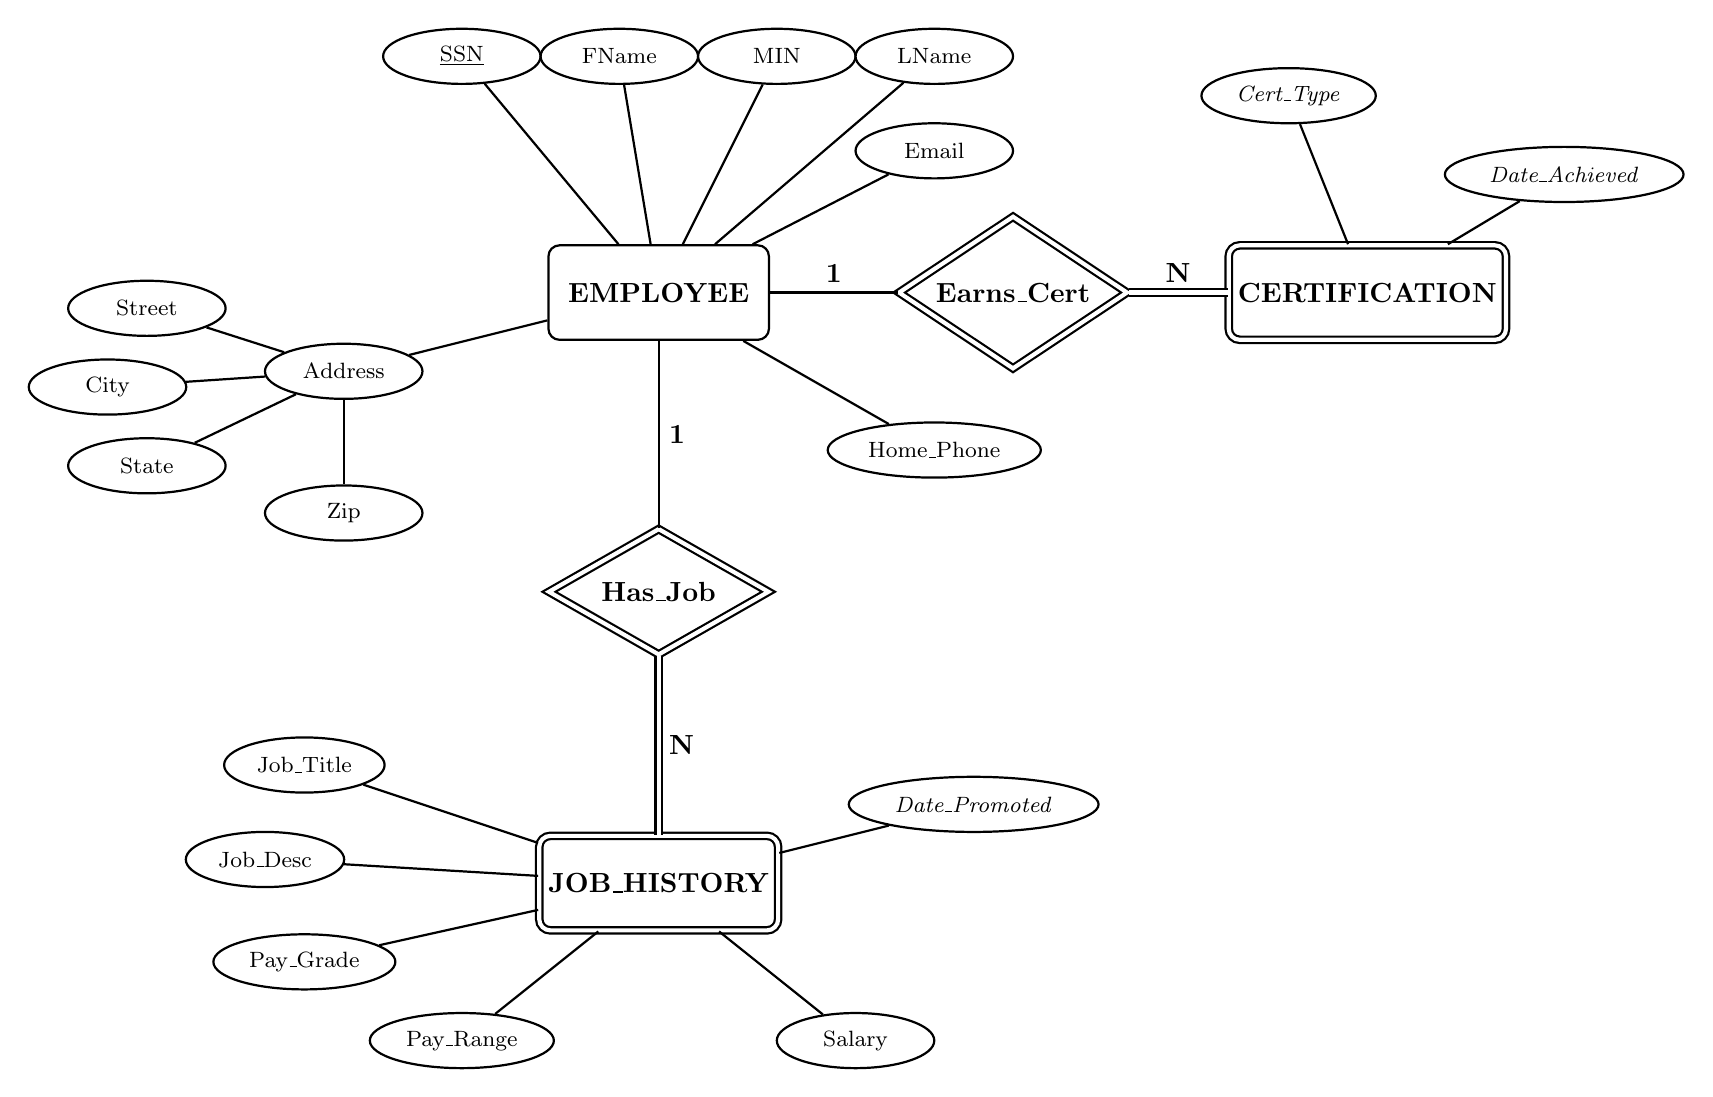
\begin{tikzpicture}[
    thick,
    entity/.style={draw, rectangle, rounded corners, minimum width=2.8cm, minimum height=1.2cm, align=center, fill=white, font=\bfseries},
    weak entity/.style={draw, double, double distance=1.5pt, rectangle, rounded corners, minimum width=2.8cm, minimum height=1.2cm, align=center, fill=white, font=\bfseries},
    relationship/.style={draw, diamond, aspect=1.5, minimum width=2.8cm, minimum height=1.2cm, align=center, fill=white, font=\bfseries},
    identifying relationship/.style={draw, double, double distance=1.5pt, diamond, aspect=1.5, minimum width=2.8cm, minimum height=1.2cm, align=center, fill=white, font=\bfseries},
    attribute/.style={draw, ellipse, minimum width=2cm, minimum height=0.7cm, align=center, fill=white, font=\footnotesize}
]

    % ================= ENTITIES & RELATIONSHIPS =================
    \node[entity] (EMP) at (0, 0) {EMPLOYEE};
    \node[weak entity] (JOB) at (0, -7.5) {JOB\_HISTORY};
    \node[weak entity] (CERT) at (9, 0) {CERTIFICATION};

    \node[identifying relationship] (HAS_JOB) at (0, -3.8) {Has\_Job};
    \node[identifying relationship] (HAS_CERT) at (4.5, 0) {Earns\_Cert};

    % ================= CONNECTIONS =================
    \draw (EMP) -- (HAS_JOB) node[midway, right, font=\bfseries] {1};
    \draw[double, double distance=1.5pt] (HAS_JOB) -- (JOB) node[midway, right, font=\bfseries] {N};

    \draw (EMP) -- (HAS_CERT) node[midway, above, font=\bfseries] {1};
    \draw[double, double distance=1.5pt] (HAS_CERT) -- (CERT) node[midway, above, font=\bfseries] {N};

    % ================= EMPLOYEE ATTRIBUTES =================
    \node[attribute] (SSN) at (-2.5, 3) {\underline{SSN}};
    \node[attribute] (FNAME) at (-0.5, 3) {FName};
    \node[attribute] (MIN) at (1.5, 3) {MIN};
    \node[attribute] (LNAME) at (3.5, 3) {LName};
    \node[attribute] (PHONE) at (3.5, -2) {Home\_Phone};
    \node[attribute] (EMAIL) at (3.5, 1.8) {Email};
    
    % Composite Address
    \node[attribute] (ADDR) at (-4, -1) {Address};
    \node[attribute] (STREET) at (-6.5, -0.2) {Street};
    \node[attribute] (CITY) at (-7, -1.2) {City};
    \node[attribute] (STATE) at (-6.5, -2.2) {State};
    \node[attribute] (ZIP) at (-4, -2.8) {Zip};

    \draw (EMP) -- (SSN);
    \draw (EMP) -- (FNAME);
    \draw (EMP) -- (MIN);
    \draw (EMP) -- (LNAME);
    \draw (EMP) -- (PHONE);
    \draw (EMP) -- (EMAIL);
    \draw (EMP) -- (ADDR);
    \draw (ADDR) -- (STREET);
    \draw (ADDR) -- (CITY);
    \draw (ADDR) -- (STATE);
    \draw (ADDR) -- (ZIP);

    % ================= JOB_HISTORY ATTRIBUTES =================
    \node[attribute] (DPROM) at (4, -6.5) {\textit{Date\_Promoted}};
    \node[attribute] (JTITLE) at (-4.5, -6) {Job\_Title};
    \node[attribute] (JDESC) at (-5, -7.2) {Job\_Desc};
    \node[attribute] (PGRADE) at (-4.5, -8.5) {Pay\_Grade};
    \node[attribute] (PRANGE) at (-2.5, -9.5) {Pay\_Range};
    \node[attribute] (SALARY) at (2.5, -9.5) {Salary};

    \draw (JOB) -- (DPROM);
    \draw (JOB) -- (JTITLE);
    \draw (JOB) -- (JDESC);
    \draw (JOB) -- (PGRADE);
    \draw (JOB) -- (PRANGE);
    \draw (JOB) -- (SALARY);

    % ================= CERTIFICATION ATTRIBUTES =================
    \node[attribute] (CTYPE) at (8, 2.5) {\textit{Cert\_Type}};
    \node[attribute] (CACH) at (11.5, 1.5) {\textit{Date\_Achieved}};

    \draw (CERT) -- (CTYPE);
    \draw (CERT) -- (CACH);

\end{tikzpicture}
}
\end{center}

\vspace{1em}
\rule{\linewidth}{0.4pt}
\vspace{1em}

\subsection*{Part (b): Relational Schema}

To yield the fewest number of relations, we apply the standard mapping rule for weak entities: the weak entity relation absorbs the primary key of its identifying strong owner entity. This eliminates the need for separate tables to represent the identifying relationships. The result is exactly \textbf{three} optimally consolidated relations.

\vspace{1em}
\begin{center}
\renewcommand{\arraystretch}{1.5}
\begin{tabular}{@{} p{3.2cm} p{8.5cm} p{3.5cm} @{}}
\toprule
\textbf{Relation} & \textbf{Attributes \small (Primary Key Underlined)} & \textbf{Foreign Keys (FK)} \\
\midrule
\textbf{EMPLOYEE} & 
\underline{SSN}, FName, MIN, LName, Street, City, State, Zip, Home\_Phone, Email & 
\textit{None} \\

\textbf{JOB\_HISTORY} & 
\underline{SSN}, \underline{Date\_Promoted}, Job\_Title, Job\_Desc, Pay\_Grade, Pay\_Range, Salary & 
\textbf{SSN} references \textbf{EMPLOYEE}(SSN) \\

\textbf{CERTIFICATION} & 
\underline{SSN}, \underline{Cert\_Type}, \underline{Date\_Achieved} & 
\textbf{SSN} references \textbf{EMPLOYEE}(SSN) \\
\bottomrule
\end{tabular}
\end{center}

\vspace{1em}
\textbf{Schema Properties:}
\begin{itemize}[leftmargin=2em, itemsep=0.3em]
    \item \textbf{EMPLOYEE:} Contains only non-multivalued attributes belonging directly to the employee.
    \item \textbf{JOB\_HISTORY:} The composite primary key \texttt{(\underline{SSN}, \underline{Date\_Promoted})} ensures that a single employee can have multiple unique job histories recorded over time without collision.
    \item \textbf{CERTIFICATION:} The composite primary key \texttt{(\underline{SSN}, \underline{Cert\_Type}, \underline{Date\_Achieved})} allows an employee to hold multiple certifications, as well as repeatedly earn the same certification on different dates.
\end{itemize}

\end{tcolorbox}

\item Consider the following scenario of a hospital:

\begin{itemize}[leftmargin=1.5em,itemsep=2pt]
  \item Patients are treated in a single ward by the doctors assigned to them. Usually each patient will be assigned a single doctor, but in rare cases he/she will be assigned two doctors.
  \item Healthcare assistants also attend to the patients; a number of these are associated with each ward.
  \item Initially the system will be concerned solely with drug treatment. Each patient is required to take a variety of drugs a certain number of times per day and for varying lengths of time.
  \item The system must record details concerning patient treatment and staff payment. Some staffs are paid on a part time basis and doctors and care assistants work varying amounts of overtime at varying rates (subject to grade).
  \item The system will also need to track what treatments are required for which patients and when, and it should be capable of calculating the cost of treatment per week for each patient.
\end{itemize}

Draw ER diagrams to show the relationships among entities of the hospital management system.
\mk{25} \yr{CSE 303 | L-3/T-1 | 2010--11}

\begin{tcolorbox}[enhanced,breakable,ansbox,colback=cA!4,colframe=cA,boxrule=0.8pt,arc=5pt,title={\textbf{Answer}},fonttitle=\bfseries\color{white},colbacktitle=cA]

\subsection*{1. Entity-Relationship (ER) Conceptual Design}

Based on the hospital scenario provided, the system can be modeled using the following entities, attributes, and relationships.

\subsubsection*{Entities and Attributes}
\begin{itemize}[leftmargin=2em, itemsep=0.3em]
    \item \textbf{STAFF (Superclass):} Generalizes common attributes for all hospital workers. 
    \begin{itemize}
        \item \textit{Attributes:} \underline{Staff\_ID} (Primary Key), Name, Grade, Is\_PartTime, OT\_Rate.
    \end{itemize}
    \item \textbf{DOCTOR (Subclass of STAFF):} Inherits from STAFF.
    \begin{itemize}
        \item \textit{Attributes:} Specialty.
    \end{itemize}
    \item \textbf{ASSISTANT (Subclass of STAFF):} Inherits from STAFF. Represents healthcare assistants.
    \begin{itemize}
        \item \textit{Attributes:} Shift.
    \end{itemize}
    \item \textbf{PATIENT:} Represents individuals admitted for treatment.
    \begin{itemize}
        \item \textit{Attributes:} \underline{Patient\_ID} (Primary Key), Name, Date\_Admitted, \textbf{\textit{Cost\_Per\_Week}} (Derived Attribute: calculated from drug unit costs and dosage frequencies).
    \end{itemize}
    \item \textbf{WARD:} The physical location where patients are treated.
    \begin{itemize}
        \item \textit{Attributes:} \underline{Ward\_No} (Primary Key), Ward\_Name, Capacity.
    \end{itemize}
    \item \textbf{DRUG:} Information regarding medicinal treatments.
    \begin{itemize}
        \item \textit{Attributes:} \underline{Drug\_Code} (Primary Key), Drug\_Name, Unit\_Cost.
    \end{itemize}
\end{itemize}

\subsubsection*{Relationships and Cardinalities}
\begin{itemize}[leftmargin=2em, itemsep=0.3em]
    \item \textbf{Admitted\_In (PATIENT $\rightarrow$ WARD):} \textbf{N:1}. Multiple patients are admitted to a single ward.
    \item \textbf{Assigned\_To (ASSISTANT $\rightarrow$ WARD):} \textbf{M:1}. Multiple healthcare assistants are associated with one specific ward.
    \item \textbf{Treats (DOCTOR $\rightarrow$ PATIENT):} \textbf{M:N}. A doctor treats multiple patients. A patient is usually assigned one doctor, but can have two (hence, inherently M:N).
    \item \textbf{Attends (ASSISTANT $\rightarrow$ PATIENT):} \textbf{M:N}. Assistants attend to multiple patients, and a patient is attended by multiple assistants.
    \item \textbf{Prescribed (PATIENT $\rightarrow$ DRUG):} \textbf{M:N}. A patient takes multiple drugs, and a drug is given to multiple patients. 
    \begin{itemize}
        \item \textit{Relationship Attributes:} Times\_Per\_Day, Duration.
    \end{itemize}
\end{itemize}

\vspace{1em}
\subsection*{2. Entity-Relationship (ER) Diagram}
\vspace{0.5em}

\begin{center}
\resizebox{\textwidth}{!}{
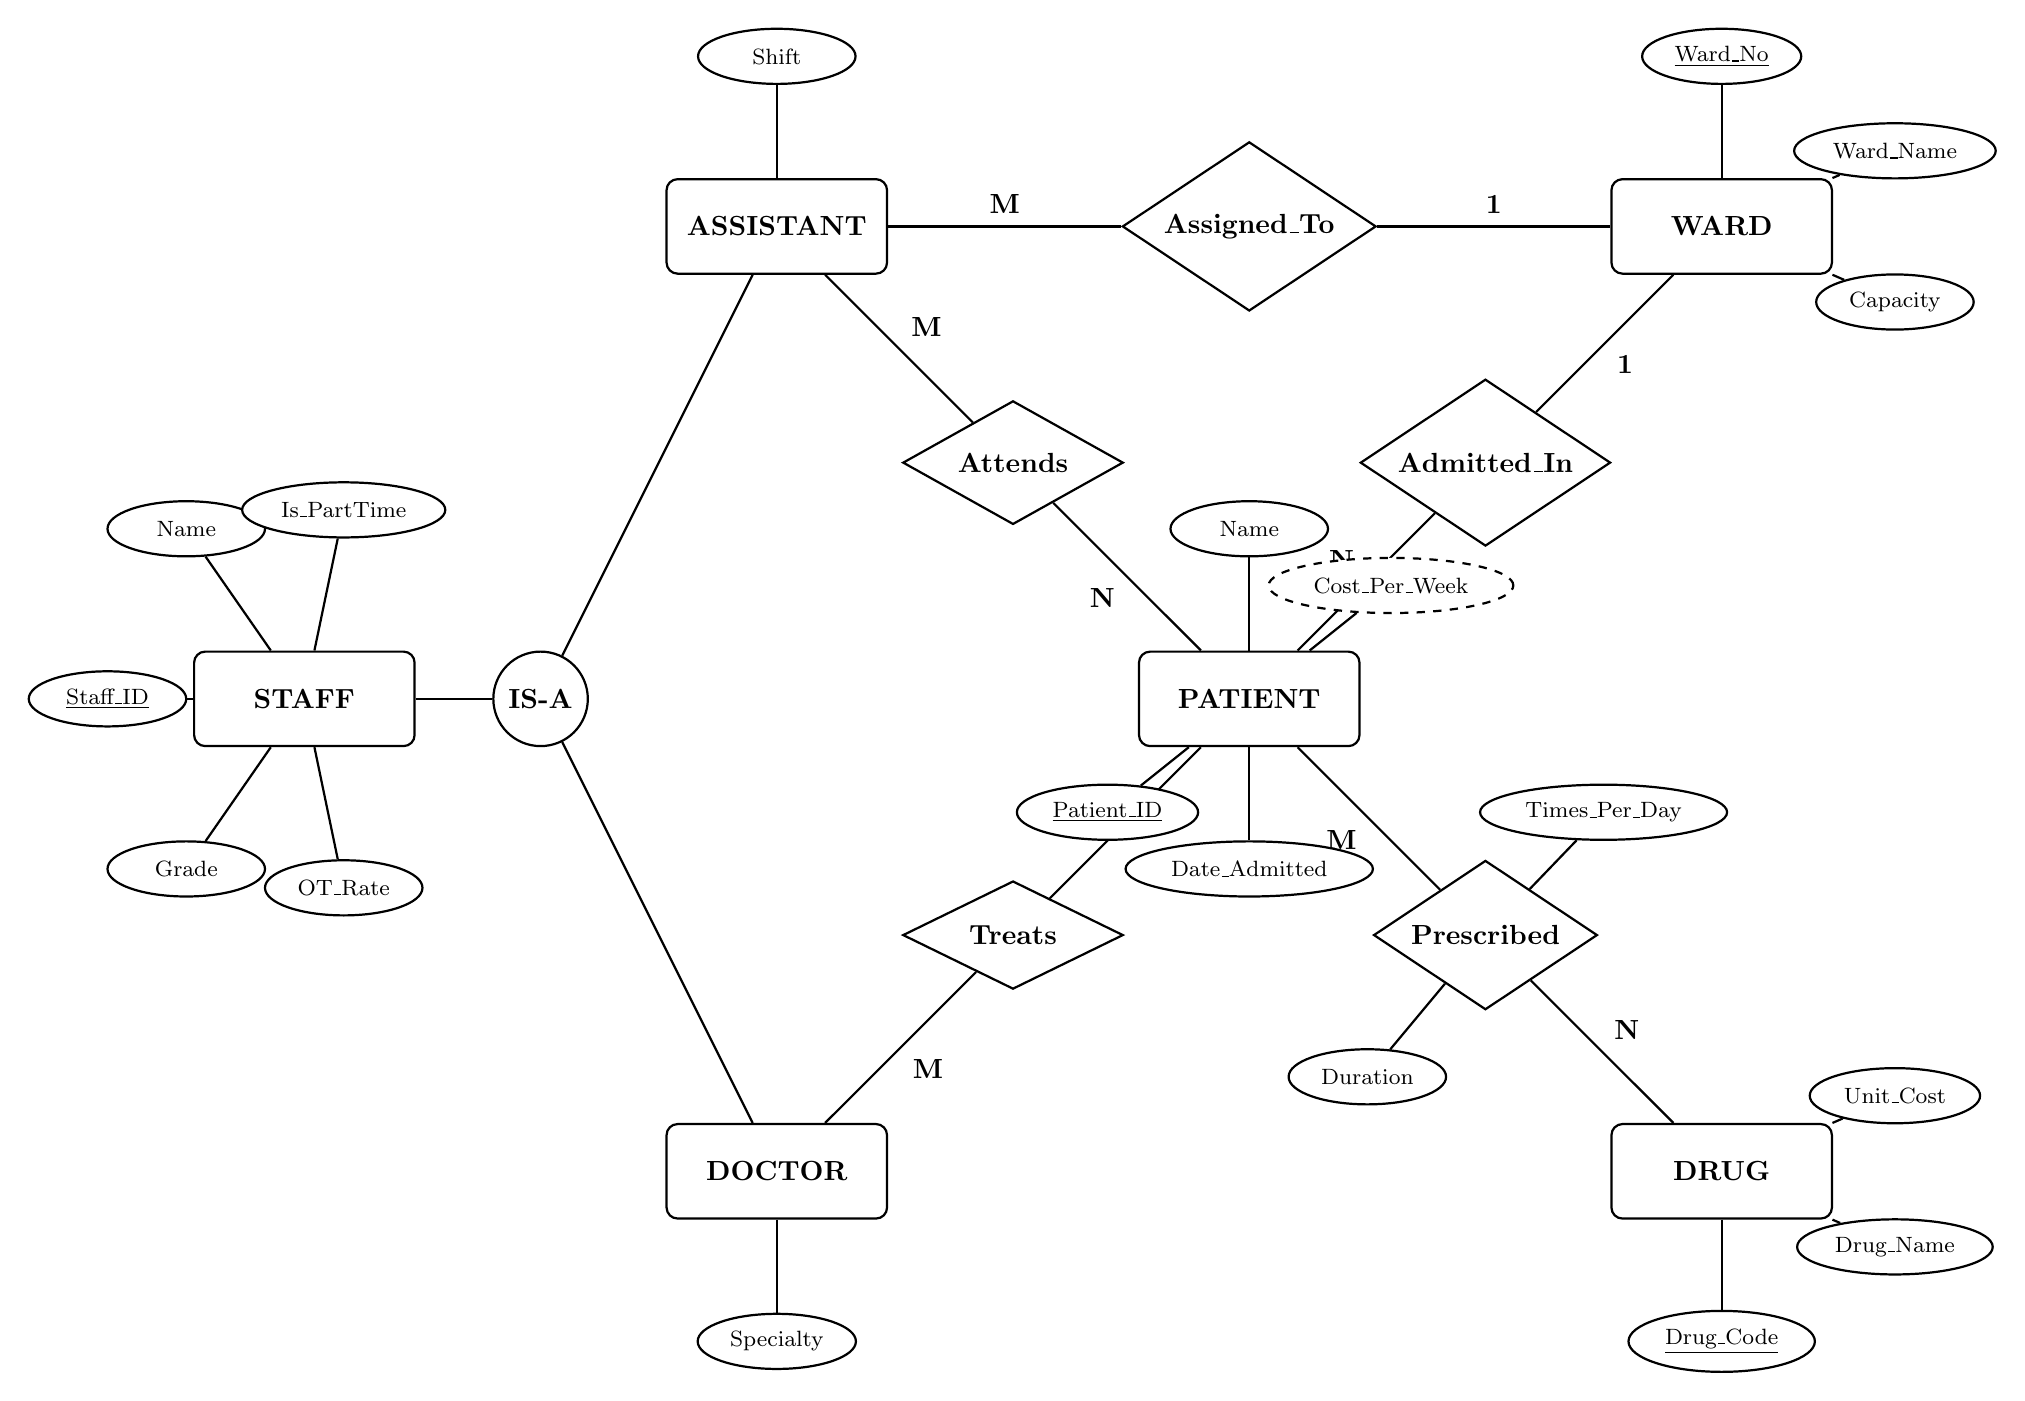
\begin{tikzpicture}[
    thick,y=1.2cm,
    entity/.style={draw, rectangle, rounded corners, minimum width=2.8cm, minimum height=1.2cm, align=center, fill=white, font=\bfseries},
    relationship/.style={draw, diamond, aspect=1.5, minimum width=2.8cm, minimum height=1.2cm, align=center, fill=white, font=\bfseries},
    attribute/.style={draw, ellipse, minimum width=2cm, minimum height=0.7cm, align=center, fill=white, font=\footnotesize},
    derived attribute/.style={draw, dashed, ellipse, minimum width=2cm, minimum height=0.7cm, align=center, fill=white, font=\footnotesize},
    isa/.style={draw, circle, minimum size=1.2cm, align=center, fill=white, font=\bfseries}
]

    % ================= ENTITIES =================
    \node[entity] (PATIENT) at (0, 0) {PATIENT};
    \node[entity] (WARD) at (6, 5) {WARD};
    \node[entity] (DRUG) at (6, -5) {DRUG};
    
    \node[entity] (STAFF) at (-12, 0) {STAFF};
    \node[entity] (ASSISTANT) at (-6, 5) {ASSISTANT};
    \node[entity] (DOCTOR) at (-6, -5) {DOCTOR};

    % ================= IS-A HIERARCHY =================
    \node[isa] (ISA) at (-9, 0) {IS-A};
    \draw (STAFF) -- (ISA);
    \draw (ISA) -- (ASSISTANT);
    \draw (ISA) -- (DOCTOR);
    
    % ================= RELATIONSHIPS =================
    \node[relationship] (ADMITTED) at (3, 2.5) {Admitted\_In};
    \node[relationship] (PRESCRIBED) at (3, -2.5) {Prescribed};
    \node[relationship] (ASSIGNED) at (0, 5) {Assigned\_To};
    \node[relationship] (ATTENDS) at (-3, 2.5) {Attends};
    \node[relationship] (TREATS) at (-3, -2.5) {Treats};

    % ================= CONNECTIONS & CARDINALITIES =================
    
    % ASSISTANT -> WARD
    \draw (ASSISTANT) -- (ASSIGNED) node[midway, above=1pt, font=\bfseries] {M};
    \draw (ASSIGNED) -- (WARD) node[midway, above=1pt, font=\bfseries] {1};

    % PATIENT -> WARD
    \draw (PATIENT) -- (ADMITTED) node[midway, above left=1pt, font=\bfseries] {N};
    \draw (ADMITTED) -- (WARD) node[midway, below right=1pt, font=\bfseries] {1};

    % PATIENT -> DRUG
    \draw (PATIENT) -- (PRESCRIBED) node[midway, below left=1pt, font=\bfseries] {M};
    \draw (PRESCRIBED) -- (DRUG) node[midway, above right=1pt, font=\bfseries] {N};

    % DOCTOR -> PATIENT
    \draw (DOCTOR) -- (TREATS) node[midway, below right=1pt, font=\bfseries] {M};
    \draw (TREATS) -- (PATIENT) node[midway, above left=1pt, font=\bfseries] {N};

    % ASSISTANT -> PATIENT
    \draw (ASSISTANT) -- (ATTENDS) node[midway, above right=1pt, font=\bfseries] {M};
    \draw (ATTENDS) -- (PATIENT) node[midway, below left=1pt, font=\bfseries] {N};

    % ================= ATTRIBUTES =================
    
    % STAFF Attributes
    \node[attribute] (st_id) at (-14.5, 0) {\underline{Staff\_ID}};
    \node[attribute] (st_name) at (-13.5, 1.8) {Name};
    \node[attribute] (st_grade) at (-13.5, -1.8) {Grade};
    \node[attribute] (st_pt) at (-11.5, 2) {Is\_PartTime};
    \node[attribute] (st_ot) at (-11.5, -2) {OT\_Rate};
    
    \draw (STAFF) -- (st_id);
    \draw (STAFF) -- (st_name);
    \draw (STAFF) -- (st_grade);
    \draw (STAFF) -- (st_pt);
    \draw (STAFF) -- (st_ot);

    % DOCTOR Attributes
    \node[attribute] (doc_spec) at (-6, -6.8) {Specialty};
    \draw (DOCTOR) -- (doc_spec);

    % ASSISTANT Attributes
    \node[attribute] (ast_shift) at (-6, 6.8) {Shift};
    \draw (ASSISTANT) -- (ast_shift);

    % PATIENT Attributes
    \node[attribute] (p_id) at (-1.8, -1.2) {\underline{Patient\_ID}};
    \node[attribute] (p_name) at (0, 1.8) {Name};
    \node[attribute] (p_date) at (0, -1.8) {Date\_Admitted};
    \node[derived attribute] (p_cost) at (1.8, 1.2) {Cost\_Per\_Week};
    
    \draw (PATIENT) -- (p_id);
    \draw (PATIENT) -- (p_name);
    \draw (PATIENT) -- (p_date);
    \draw (PATIENT) -- (p_cost);

    % WARD Attributes
    \node[attribute] (w_no) at (6, 6.8) {\underline{Ward\_No}};
    \node[attribute] (w_name) at (8.2, 5.8) {Ward\_Name};
    \node[attribute] (w_cap) at (8.2, 4.2) {Capacity};
    
    \draw (WARD) -- (w_no);
    \draw (WARD) -- (w_name);
    \draw (WARD) -- (w_cap);

    % DRUG Attributes
    \node[attribute] (d_code) at (6, -6.8) {\underline{Drug\_Code}};
    \node[attribute] (d_name) at (8.2, -5.8) {Drug\_Name};
    \node[attribute] (d_cost) at (8.2, -4.2) {Unit\_Cost};
    
    \draw (DRUG) -- (d_code);
    \draw (DRUG) -- (d_name);
    \draw (DRUG) -- (d_cost);

    % PRESCRIBED Relationship Attributes
    \node[attribute] (r_times) at (4.5, -1.2) {Times\_Per\_Day};
    \node[attribute] (r_dur) at (1.5, -4) {Duration};
    
    \draw (PRESCRIBED) -- (r_times);
    \draw (PRESCRIBED) -- (r_dur);

\end{tikzpicture}
}
\end{center}

\end{tcolorbox}

%% Q2
\end{enumerate}

%%──────────────────────────────────────────────────────────────────────
\subtopic{cA}{Database Schema Design}
\label{sub:s2-schema}

\begin{enumerate}

%% Q1
\item Write the general procedure to convert a ternary relationship to binary relationships.
\mk{8} \yr{CSE 215 | L-2/T-1 | 2024--25}

\begin{tcolorbox}[enhanced,breakable,ansbox,colback=cA!4,colframe=cA,boxrule=0.8pt,arc=5pt,title={\textbf{Answer}},fonttitle=\bfseries\color{white},colbacktitle=cA]

\subsection*{Conversion of a Ternary Relationship to Binary Relationships}

In database design, a \textbf{ternary relationship} exists when three distinct entities participate in a single relationship. However, many implementation data models (and some design tools) restrict relationships to be strictly \textbf{binary} (degree 2). To resolve this, a ternary relationship must be decomposed into equivalent binary relationships using an \textbf{associative entity} (or weak entity).

\subsubsection*{General Procedure}

The systematic procedure to convert a ternary relationship $R$ connecting three entity types $A$, $B$, and $C$ into binary relationships involves the following steps:

\begin{enumerate}
    \item \textbf{Create an Associative Entity:} 
    Create a new entity type, let's call it $E_R$, to represent the ternary relationship. This new entity is inherently existence-dependent on the original entities, often making it a weak entity.
    
    \item \textbf{Establish Binary Relationships:} 
    Remove the original ternary relationship $R$. Create three new binary relationships (e.g., $R_A$, $R_B$, and $R_C$) that connect the newly created associative entity $E_R$ to each of the three original participating entities $A$, $B$, and $C$.
    
    \item \textbf{Assign Cardinalities:} 
    The relationship between the original entities and the new associative entity will always be \textbf{1:N} (One-to-Many). 
    \begin{itemize}
        \item The original entities ($A$, $B$, and $C$) will have a cardinality of \textbf{1}.
        \item The associative entity ($E_R$) will have a cardinality of \textbf{N} in all three binary relationships.
    \end{itemize}
    
    \item \textbf{Migrate Attributes:} 
    Any descriptive attributes that originally belonged to the ternary relationship $R$ must be moved to the new associative entity $E_R$.
    
    \item \textbf{Define the Primary Key:} 
    The primary key of the new associative entity $E_R$ is formed by the combination (concatenation) of the primary keys of the participating entities $A$, $B$, and $C$. If $R$ had its own partial key or discriminators, they are also included.
    \[ PK(E_R) = PK(A) \cup PK(B) \cup PK(C) \]
\end{enumerate}

\vspace{1em}
\subsubsection*{Visual Representation (ER Diagram Conversion)}

The following diagram illustrates the transformation from a ternary relationship to three binary relationships linked by an associative entity.

\vspace{1em}
\begin{center}
\resizebox{0.9\textwidth}{!}{
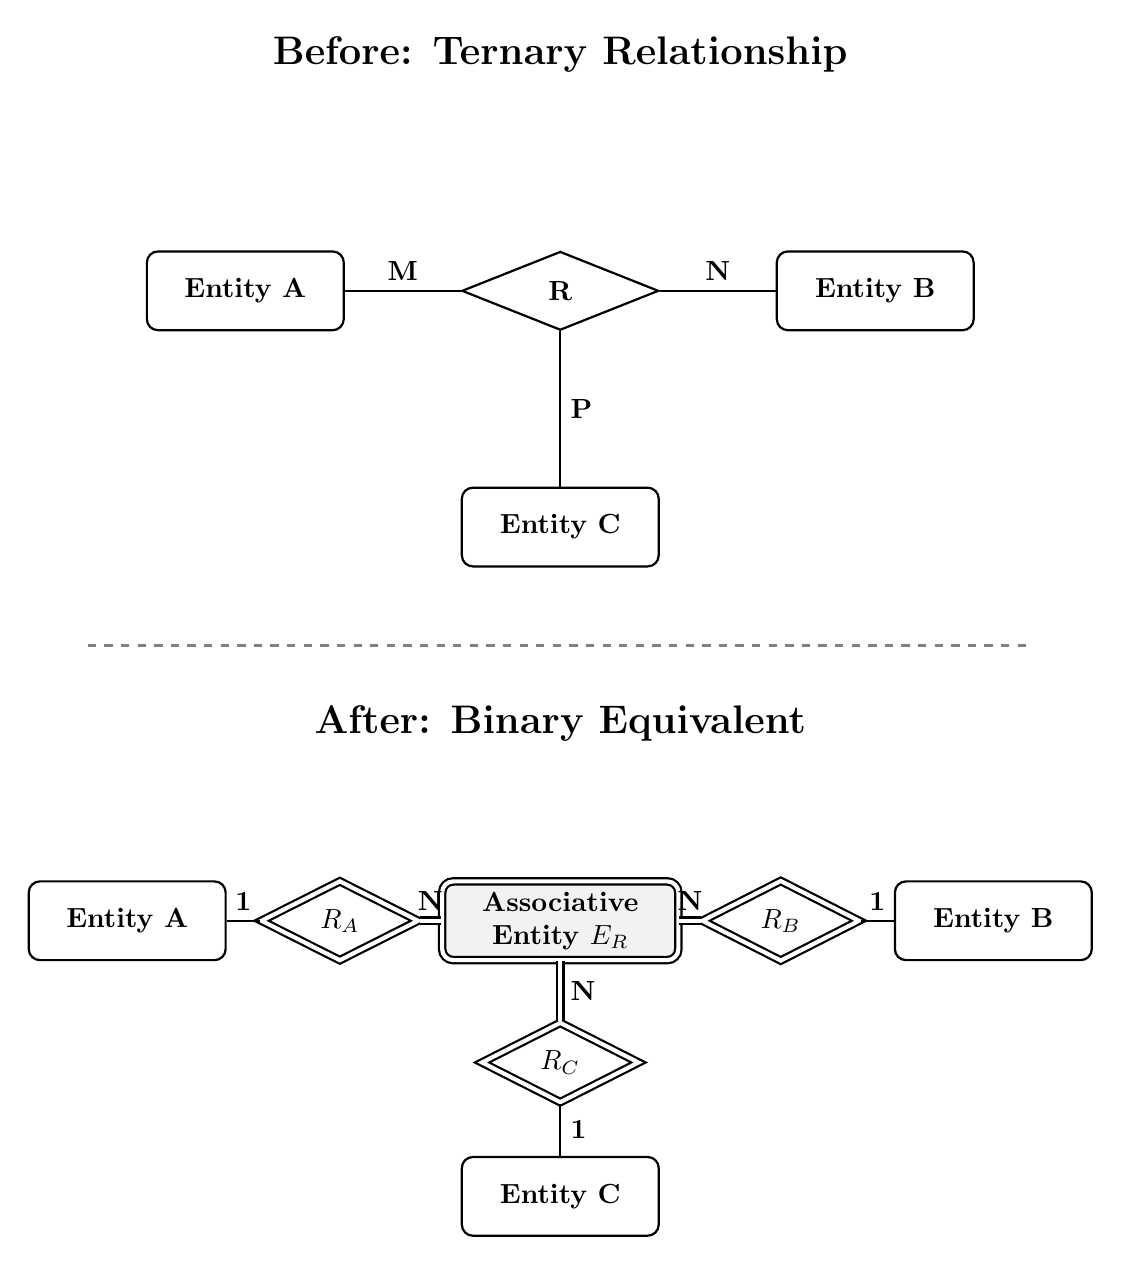
\begin{tikzpicture}[
    thick,
    entity/.style={draw, rectangle, rounded corners, minimum width=2.5cm, minimum height=1cm, align=center, fill=white, font=\bfseries},
    associative/.style={draw, double, double distance=1.5pt, rectangle, rounded corners, minimum width=3cm, minimum height=1cm, align=center, fill=gray!10, font=\bfseries},
    relationship/.style={draw, diamond, aspect=1.5, minimum width=2.5cm, minimum height=1cm, align=center, fill=white, font=\bfseries},
    id_relationship/.style={draw, double, double distance=1.5pt, diamond, aspect=1.5, minimum width=2cm, minimum height=1cm, align=center, fill=white, font=\bfseries},
    label_style/.style={font=\bfseries, text=black}
]

    % ================= TERNARY (BEFORE) =================
    \node[font=\bfseries\Large] at (0, 3) {Before: Ternary Relationship};

    \node[entity] (A1) at (-4, 0) {Entity A};
    \node[entity] (B1) at (4, 0) {Entity B};
    \node[entity] (C1) at (0, -3) {Entity C};
    \node[relationship] (R1) at (0, 0) {R};

    \draw (A1) -- (R1) node[midway, above, label_style] {M};
    \draw (B1) -- (R1) node[midway, above, label_style] {N};
    \draw (C1) -- (R1) node[midway, right, label_style] {P};

    % Separator Line
    \draw[dashed, draw=gray, line width=1pt] (-6, -4.5) -- (6, -4.5);

    % ================= BINARY (AFTER) =================
    \node[font=\bfseries\Large] at (0, -5.5) {After: Binary Equivalent};

    \node[entity] (A2) at (-5.5, -8) {Entity A};
    \node[entity] (B2) at (5.5, -8) {Entity B};
    \node[entity] (C2) at (0, -11.5) {Entity C};
    
    \node[associative] (ER) at (0, -8) {Associative\\Entity $E_R$};
    
    \node[id_relationship] (RA) at (-2.8, -8) {$R_A$};
    \node[id_relationship] (RB) at (2.8, -8) {$R_B$};
    \node[id_relationship] (RC) at (0, -9.8) {$R_C$};

    % Connections and Cardinalities for A
    \draw (A2) -- (RA) node[midway, above, label_style] {1};
    \draw[double, double distance=1.5pt] (RA) -- (ER) node[midway, above, label_style] {N};

    % Connections and Cardinalities for B
    \draw (B2) -- (RB) node[midway, above, label_style] {1};
    \draw[double, double distance=1.5pt] (RB) -- (ER) node[midway, above, label_style] {N};

    % Connections and Cardinalities for C
    \draw (C2) -- (RC) node[midway, right, label_style] {1};
    \draw[double, double distance=1.5pt] (RC) -- (ER) node[midway, right, label_style] {N};

\end{tikzpicture}
}
\end{center}

\vspace{1em}
\subsubsection*{Relational Schema Mapping (Example)}

If the entities $A$, $B$, and $C$ have primary keys $A\_ID$, $B\_ID$, and $C\_ID$ respectively, and the ternary relationship $R$ has an attribute \textit{Date}, the resulting relational schema will be:

\begin{itemize}
    \item \textbf{Entity A:} ( \underline{A\_ID}, \dots )
    \item \textbf{Entity B:} ( \underline{B\_ID}, \dots )
    \item \textbf{Entity C:} ( \underline{C\_ID}, \dots )
    \item \textbf{Associative Entity $\mathbf{E_R}$:} ( \underline{A\_ID}, \underline{B\_ID}, \underline{C\_ID}, Date )
\end{itemize}
\textit{Note: In the associative entity $E_R$, the combination of foreign keys ($A\_ID$, $B\_ID$, $C\_ID$) serves as its composite primary key.}

\end{tcolorbox}

\item Explain the concept of total and partial participation of entities in a relationship set using an example ER diagram.
\mk{10} \yr{CSE 215 | L-2/T-1 | 2024--25}

\begin{tcolorbox}[enhanced,breakable,ansbox,colback=cA!4,colframe=cA,boxrule=0.8pt,arc=5pt,title={\textbf{Answer}},fonttitle=\bfseries\color{white},colbacktitle=cA]

\subsection*{Participation Constraints in Entity-Relationship (ER) Models}

In an ER model, a \textbf{participation constraint} (also known as a minimum cardinality constraint) specifies whether the existence of an entity depends on its being related to another entity via a relationship type. It defines the minimum number of relationship instances that each entity must participate in. 

There are two types of participation constraints: \textbf{Total} and \textbf{Partial}.

\subsubsection*{1. Total Participation (Existence Dependency)}
\begin{itemize}
    \item \textbf{Definition:} An entity set has total participation in a relationship set if \textbf{every} entity in the entity set is associated with at least one entity in the other entity set through that relationship.
    \item \textbf{Explanation:} The existence of the entity dictates that it must be related to something else. If an entity does not participate in the relationship, it cannot exist in the database.
    \item \textbf{Notation:} Represented by a \textbf{double line} connecting the entity rectangle to the relationship diamond.
\end{itemize}

\subsubsection*{2. Partial Participation}
\begin{itemize}
    \item \textbf{Definition:} An entity set has partial participation if \textbf{only some} entities in the entity set are associated with entities in the other entity set.
    \item \textbf{Explanation:} Participation is optional. An entity can exist in the database without participating in the relationship.
    \item \textbf{Notation:} Represented by a \textbf{single line} connecting the entity rectangle to the relationship diamond.
\end{itemize}

\vspace{1em}
\subsubsection*{Example Scenario}

Consider the entities \textbf{EMPLOYEE} and \textbf{DEPARTMENT}, and the relationship \textbf{Manages}:
\begin{itemize}
    \item Not every employee is a manager. Therefore, the participation of \textbf{EMPLOYEE} in the \textbf{Manages} relationship is \textbf{partial}.
    \item However, every department must have a manager to function. Therefore, the participation of \textbf{DEPARTMENT} in the \textbf{Manages} relationship is \textbf{total}.
\end{itemize}

\vspace{1em}
\begin{center}
\resizebox{0.85\textwidth}{!}{
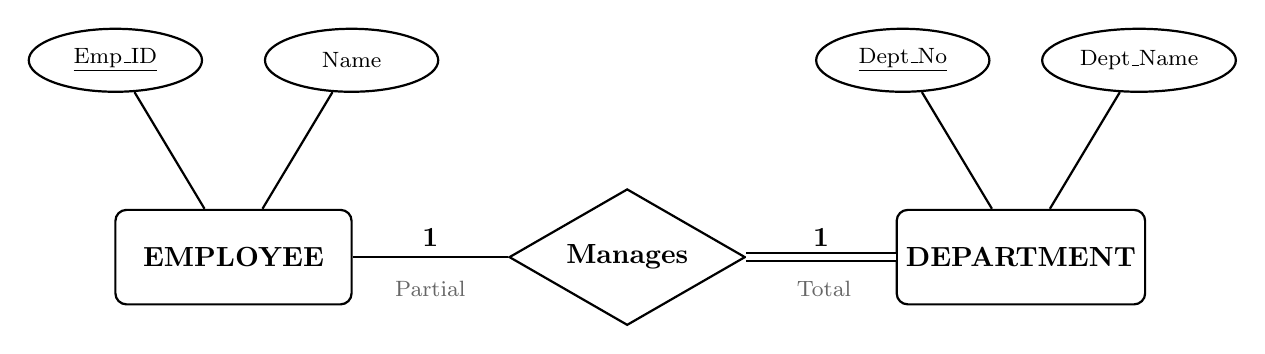
\begin{tikzpicture}[
    thick,
    entity/.style={draw, rectangle, rounded corners, minimum width=3cm, minimum height=1.2cm, align=center, fill=white, font=\bfseries},
    relationship/.style={draw, diamond, aspect=1.5, minimum width=3cm, minimum height=1.2cm, align=center, fill=white, font=\bfseries},
    attribute/.style={draw, ellipse, minimum width=2.2cm, minimum height=0.8cm, align=center, fill=white, font=\footnotesize}
]

    % Entities and Relationship
    \node[entity] (EMP) at (-5, 0) {EMPLOYEE};
    \node[relationship] (MANAGES) at (0, 0) {Manages};
    \node[entity] (DEPT) at (5, 0) {DEPARTMENT};

    % Relationships links (Partial and Total)
    % Partial participation (Single line)
    \draw (EMP) -- (MANAGES) node[midway, above, font=\bfseries] {1};
    \node[font=\footnotesize, text=gray!80!black] at (-2.5, -0.4) {Partial};
    
    % Total participation (Double line)
    \draw[double, double distance=2pt] (MANAGES) -- (DEPT) node[midway, above, font=\bfseries] {1};
    \node[font=\footnotesize, text=gray!80!black] at (2.5, -0.4) {Total};

    % Attributes for EMPLOYEE
    \node[attribute] (E_ID) at (-6.5, 2.5) {\underline{Emp\_ID}};
    \node[attribute] (E_NAME) at (-3.5, 2.5) {Name};
    
    \draw (EMP) -- (E_ID);
    \draw (EMP) -- (E_NAME);

    % Attributes for DEPARTMENT
    \node[attribute] (D_NO) at (3.5, 2.5) {\underline{Dept\_No}};
    \node[attribute] (D_NAME) at (6.5, 2.5) {Dept\_Name};
    
    \draw (DEPT) -- (D_NO);
    \draw (DEPT) -- (D_NAME);

\end{tikzpicture}
}
\end{center}
\vspace{1em}

\subsubsection*{Comparison Table}

\begin{center}
\renewcommand{\arraystretch}{1.4}
\begin{tabular}{@{} l p{6cm} p{6cm} @{}}
\toprule
\textbf{Feature} & \textbf{Total Participation} & \textbf{Partial Participation} \\
\midrule
\textbf{Mandatory/Optional} & Mandatory (must participate) & Optional (may or may not participate) \\
\textbf{Existence Dependency} & Yes. Entity cannot exist without the relationship. & No. Entity can exist independently of the relationship. \\
\textbf{ER Notation} & Double continuous line & Single continuous line \\
\textbf{Minimum Cardinality} & Minimum constraint is $\ge 1$ & Minimum constraint is $0$ \\
\bottomrule
\end{tabular}
\end{center}

\end{tcolorbox}

\item How are composite attributes and multivalued attributes handled when an ER model is transformed into a relational database schema? Explain with examples.
\mk{10} \yr{CSE 215 | L-2/T-1 | 2024--25}

\begin{tcolorbox}[enhanced,breakable,ansbox,colback=cA!4,colframe=cA,boxrule=0.8pt,arc=5pt,title={\textbf{Answer}},fonttitle=\bfseries\color{white},colbacktitle=cA]

\subsection*{Transformation of Composite and Multivalued Attributes}

When mapping an Entity-Relationship (ER) model to a relational database schema, different types of attributes require distinct transformation rules to satisfy the principles of normalization (specifically First Normal Form, which requires atomic values).

---

\subsubsection*{1. Handling Composite Attributes}

\textbf{Rule:} A composite attribute is \textbf{flattened}. Only its simple, component sub-attributes are included as columns in the resulting relation. The parent composite attribute itself is discarded and does not appear in the relational schema.

\begin{itemize}
    \item \textbf{Working Principle:} The relational model does not support nested structures or attributes containing sub-attributes. By extracting the leaf-level atomic attributes, the relation remains in First Normal Form (1NF).
    \item \textbf{Example:} Consider an entity \textbf{EMPLOYEE} with a primary key \textit{Emp\_ID} and a composite attribute \textit{Name} comprising \textit{Fname}, \textit{Minit}, and \textit{Lname}.
\end{itemize}

\vspace{0.5em}
\begin{center}
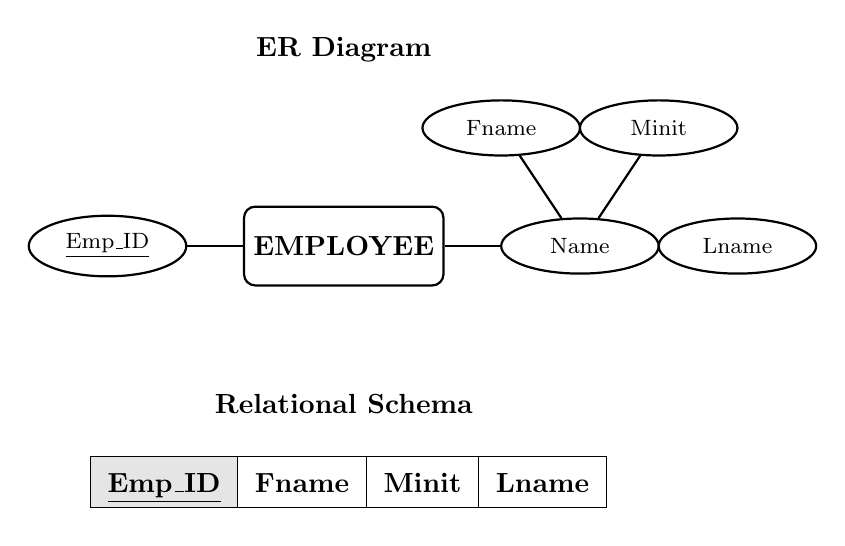
\begin{tikzpicture}[
    thick,
    entity/.style={draw, rectangle, rounded corners, minimum width=2.5cm, minimum height=1cm, align=center, fill=white, font=\bfseries},
    attribute/.style={draw, ellipse, minimum width=2cm, minimum height=0.7cm, align=center, fill=white, font=\footnotesize}
]
    % ER Diagram
    \node[font=\bfseries] at (0, 2.5) {ER Diagram};
    
    \node[entity] (emp) at (0, 0) {EMPLOYEE};
    \node[attribute] (eid) at (-3, 0) {\underline{Emp\_ID}};
    \node[attribute] (name) at (3, 0) {Name};
    
    \node[attribute] (fname) at (2, 1.5) {Fname};
    \node[attribute] (minit) at (4, 1.5) {Minit};
    \node[attribute] (lname) at (5, 0) {Lname};

    \draw (emp) -- (eid);
    \draw (emp) -- (name);
    \draw (name) -- (fname);
    \draw (name) -- (minit);
    \draw (name) -- (lname);

    % Relational Schema
    \node[font=\bfseries] at (0, -2) {Relational Schema};
    
    \node at (0, -3) {
        \renewcommand{\arraystretch}{1.5}
        \begin{tabular}{|c|c|c|c|}
        \hline
        \cellcolor{gray!20}\textbf{\underline{Emp\_ID}} & \textbf{Fname} & \textbf{Minit} & \textbf{Lname} \\
        \hline
        \end{tabular}
    };
\end{tikzpicture}
\end{center}

---

\subsubsection*{2. Handling Multivalued Attributes}

\textbf{Rule:} A multivalued attribute cannot be stored in a single column because it violates 1NF. It is transformed by creating a \textbf{new, separate relation} (table). 

\begin{itemize}
    \item \textbf{Working Principle:} 
    \begin{enumerate}
        \item Create a new relation to hold the multivalued data.
        \item Include a column for the multivalued attribute itself.
        \item Add the primary key of the parent entity as a \textbf{Foreign Key (FK)} in this new relation.
        \item The \textbf{Primary Key (PK)} of the new relation is formed by the \textbf{combination} of the foreign key and the multivalued attribute.
    \end{enumerate}
    \item \textbf{Example:} Consider an entity \textbf{EMPLOYEE} with a primary key \textit{Emp\_ID} and a multivalued attribute \textit{Phone}.
\end{itemize}

\vspace{0.5em}
\begin{center}
    % ==========================================
    % PART 1: ER DIAGRAM (Using TikZ)
    % ==========================================
    \textbf{\Large ER Diagram}\\[1.5em]
    
    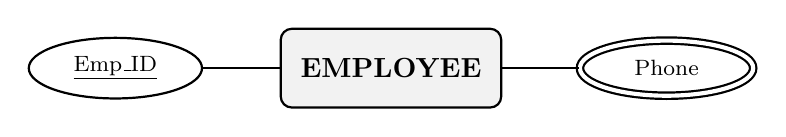
\begin{tikzpicture}[
        thick,
        entity/.style={draw, rectangle, rounded corners,minimum width=2.8cm, minimum height=1cm, align=center, fill=black!5, font=\bfseries},
        attribute/.style={draw, ellipse, minimum width=2.2cm, minimum height=0.7cm, align=center, rounded corners,fill=white, font=\footnotesize},
        multi_attribute/.style={draw, rounded corners,double, double distance=1.5pt, ellipse, minimum width=2.2cm, minimum height=0.7cm, align=center, fill=white, font=\footnotesize}
    ]
        % Nodes
        \node[entity] (emp) at (0, 0) {EMPLOYEE};
        \node[attribute] (eid) at (-3.5, 0) {\underline{Emp\_ID}};
        \node[multi_attribute] (phone) at (3.5, 0) {Phone};

        % Edges
        \draw (emp) -- (eid);
        \draw (emp) -- (phone);
    \end{tikzpicture}

    \vspace{3em}

    % ==========================================
    % PART 2: RELATIONAL SCHEMA (Using Tabular)
    % ==========================================
    \textbf{\Large Relational Schema}\\[1.5em]
    
    \renewcommand{\arraystretch}{1.8} % Spacious rows

    % EMPLOYEE Table
    \begin{tabular}{|>{\columncolor{black!10}\bfseries\centering\arraybackslash}m{3.2cm}|>{\centering\arraybackslash}m{3.2cm}|}
        \hline
        EMPLOYEE & \underline{\textbf{Emp\_ID}} \\
        \hline
    \end{tabular}

    \vspace{1.5em}
    
    % EMP_PHONE Table (Multi-valued attribute mapped to a new table)
    \begin{tabular}{|>{\columncolor{black!10}\bfseries\centering\arraybackslash}m{3.2cm}|>{\centering\arraybackslash}m{3.2cm}|>{\centering\arraybackslash}m{3.2cm}|}
        \hline
        EMP\_PHONE & \underline{\textbf{Emp\_ID}} \newline \scriptsize(FK) & \underline{\textbf{Phone}} \\
        \hline
    \end{tabular}

\end{center}

\vspace{0.5em}

% ==========================================
% PART 3: SCHEMA CONSTRAINTS & NOTES
% ==========================================
\begin{flushleft}
    \footnotesize\textit{* \textbf{Composite Primary Key:} The primary key for EMP\_PHONE is (\textbf{Emp\_ID}, \textbf{Phone}).}\\
    \footnotesize\textit{** \textbf{Foreign Key Mapping:} EMP\_PHONE.\textbf{Emp\_ID} $\rightarrow$ EMPLOYEE.\textbf{Emp\_ID}}
\end{flushleft}

---

\subsubsection*{Summary Comparison}

\begin{center}
\begin{tabular}{@{} p{3.5cm} p{6cm} p{5.5cm} @{}}
\toprule
\textbf{Attribute Type} & \textbf{Transformation Action} & \textbf{Result in Schema} \\
\midrule
\textbf{Composite} & Flatten the components. Drop the parent attribute. & Additional columns in the \textit{same} original table. \\
\addlinespace
\textbf{Multivalued} & Create a completely new relation. & A \textit{new} table linked via a Foreign Key, forming a composite Primary Key. \\
\bottomrule
\end{tabular}
\end{center}

\end{tcolorbox}

\item A library keeps records of current loans of books to borrowers. Each borrower is identified by a borrower number; each copy of a book by an accession number. The library may hold more than one copy of any given book. Borrower name and address are stored for communications. Book information includes: title, author name(s), publisher name, publication date, ISBN, purchase price, classification (reference or fiction), and number of pages. A book may be written by multiple authors but published by a single publisher. The library uses unique in-house codes for authors and publishers. A book may cover multiple subjects; borrowers can use an online catalogue to select texts by subject, title, or author. There are restrictions on the number of books a borrower may have on loan and the loan period, depending on borrower classification (junior, adult, or organization). When a book is borrowed, the return date is automatically recorded. Other borrowers may reserve books currently on loan; the reservation date is recorded. A borrower status flag is maintained --- borrowers who hold overdue books or have reached their loan limit are flagged to prevent further borrowings.
\begin{enumerate}
  \item Draw an Entity-Relationship (ER) diagram to represent the library data requirements described above.
  \item Identify two attributes in the above scenario which can be derived using business rules. Write the schema description to store these business rules.
\end{enumerate}
\mk{26} \yr{CSE 215 | L-2/T-1 | 2023--24}

\begin{tcolorbox}[enhanced,breakable,ansbox,colback=cA!4,colframe=cA,boxrule=0.8pt,arc=5pt,title={\textbf{Answer}},fonttitle=\bfseries\color{white},colbacktitle=cA]

\subsection*{1. Entity-Relationship (ER) Diagram}

Based on the library requirements, the conceptual data model involves central entities like \textbf{BOOK}, \textbf{COPY}, and \textbf{BORROWER}. Standard normalization rules are applied to extract \textbf{AUTHOR}, \textbf{PUBLISHER}, and \textbf{SUBJECT} into separate entities to accommodate their respective relationships (M:N for authors and subjects, 1:N for publishers). 

\vspace{1em}
\begin{center}
\resizebox{\textwidth}{!}{
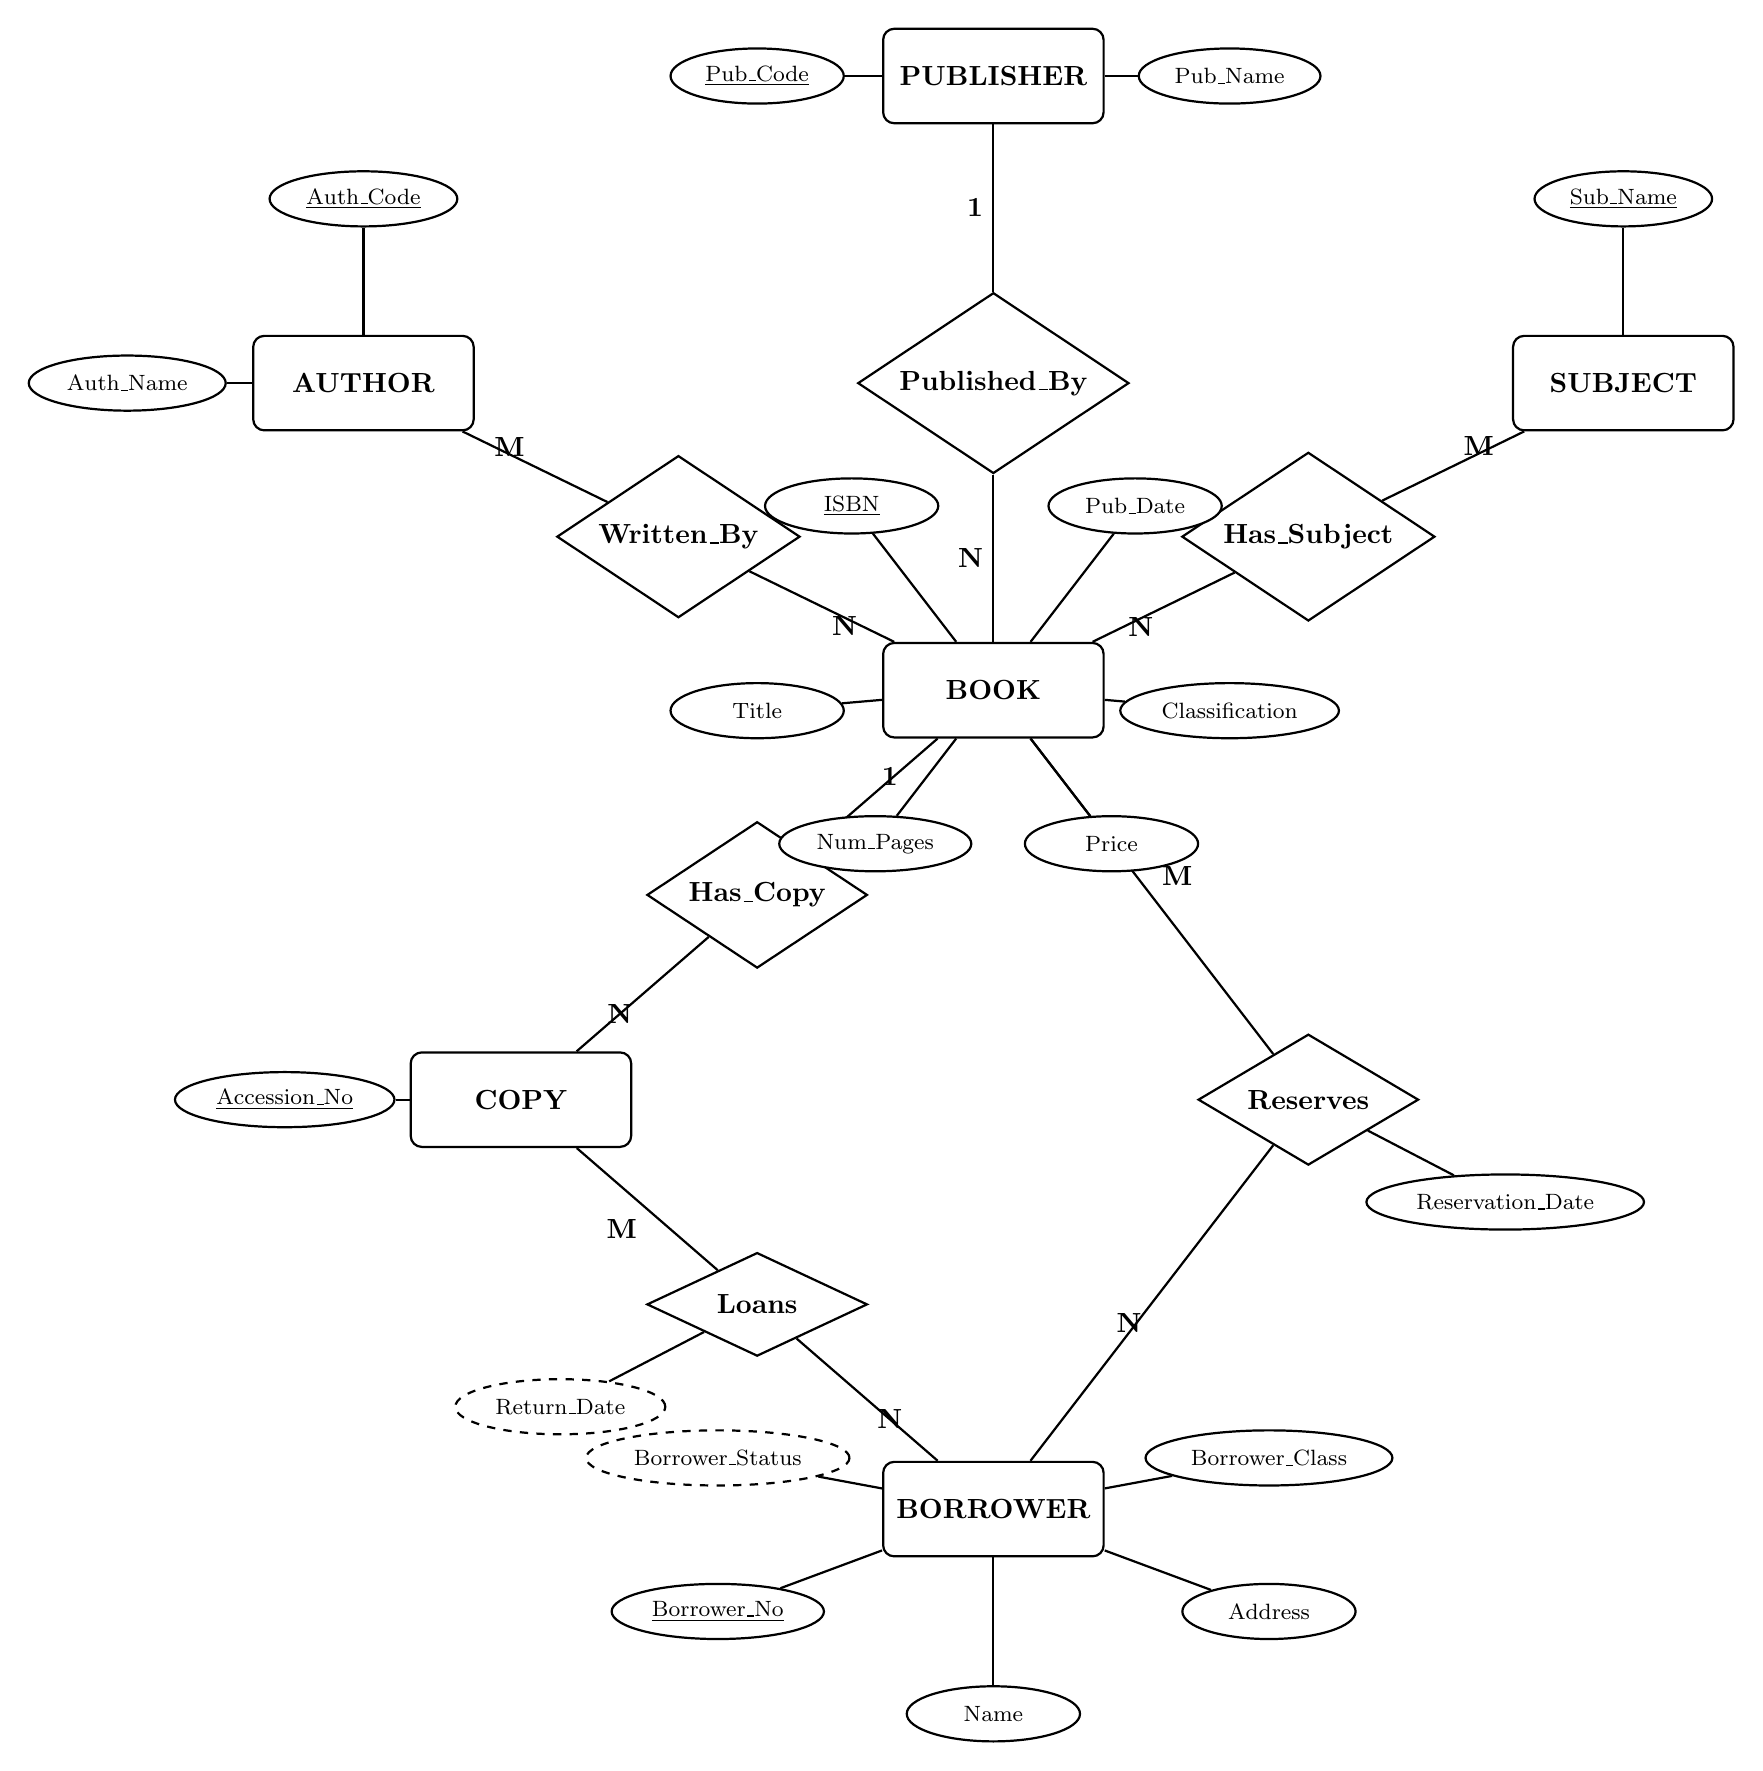
\begin{tikzpicture}[
    thick,y=1.3cm,
    entity/.style={draw, rectangle, rounded corners, minimum width=2.8cm, minimum height=1.2cm, align=center, fill=white, font=\bfseries},
    relationship/.style={draw, diamond, aspect=1.5, minimum width=2.8cm, minimum height=1.2cm, align=center, fill=white, font=\bfseries},
    attribute/.style={draw, ellipse, minimum width=2.2cm, minimum height=0.7cm, align=center, fill=white, font=\footnotesize},
    derived_attribute/.style={draw, dashed, ellipse, minimum width=2.2cm, minimum height=0.7cm, align=center, fill=white, font=\footnotesize},
    card/.style={font=\bfseries, text=black}
]

    % ================= ENTITIES =================
    \node[entity] (BOOK) at (0, 0) {BOOK};
    \node[entity] (PUB) at (0, 6) {PUBLISHER};
    \node[entity] (AUTH) at (-8, 3) {AUTHOR};
    \node[entity] (SUBJ) at (8, 3) {SUBJECT};
    \node[entity] (COPY) at (-6, -4) {COPY};
    \node[entity] (BORR) at (0, -8) {BORROWER};

    % ================= RELATIONSHIPS =================
    \node[relationship] (PUB_BY) at (0, 3) {Published\_By};
    \node[relationship] (WRIT_BY) at (-4, 1.5) {Written\_By};
    \node[relationship] (HAS_SUBJ) at (4, 1.5) {Has\_Subject};
    \node[relationship] (HAS_COPY) at (-3, -2) {Has\_Copy};
    \node[relationship] (LOANS) at (-3, -6) {Loans};
    \node[relationship] (RESERVES) at (4, -4) {Reserves};

    % ================= EDGES & CARDINALITIES =================
    
    % Publisher to Book (1:N)
    \draw (PUB) -- (PUB_BY) node[midway, left, card] {1};
    \draw (PUB_BY) -- (BOOK) node[midway, left, card] {N};

    % Author to Book (M:N)
    \draw (AUTH) -- (WRIT_BY) node[midway, above left, card] {M};
    \draw (WRIT_BY) -- (BOOK) node[midway, below right, card] {N};

    % Subject to Book (M:N)
    \draw (SUBJ) -- (HAS_SUBJ) node[midway, above right, card] {M};
    \draw (HAS_SUBJ) -- (BOOK) node[midway, below left, card] {N};

    % Book to Copy (1:N)
    \draw (BOOK) -- (HAS_COPY) node[midway, above right, card] {1};
    \draw (HAS_COPY) -- (COPY) node[midway, below left, card] {N};

    % Copy to Borrower (Loans M:N)
    \draw (COPY) -- (LOANS) node[midway, below left, card] {M};
    \draw (LOANS) -- (BORR) node[midway, below right, card] {N};

    % Book to Borrower (Reserves M:N)
    \draw (BOOK) -- (RESERVES) node[midway, above right, card] {M};
    \draw (RESERVES) -- (BORR) node[midway, below left, card] {N};

    % ================= ATTRIBUTES =================
    
    % PUBLISHER Attributes
    \node[attribute] (pub_code) at (-3, 6) {\underline{Pub\_Code}};
    \node[attribute] (pub_name) at (3, 6) {Pub\_Name};
    \draw (PUB) -- (pub_code);
    \draw (PUB) -- (pub_name);

    % AUTHOR Attributes
    \node[attribute] (auth_code) at (-8, 4.8) {\underline{Auth\_Code}};
    \node[attribute] (auth_name) at (-11, 3) {Auth\_Name};
    \draw (AUTH) -- (auth_code);
    \draw (AUTH) -- (auth_name);

    % SUBJECT Attributes
    \node[attribute] (sub_name) at (8, 4.8) {\underline{Sub\_Name}};
    \draw (SUBJ) -- (sub_name);

    % BOOK Attributes
    \node[attribute] (isbn) at (-1.8, 1.8) {\underline{ISBN}};
    \node[attribute] (title) at (-3, -0.2) {Title};
    \node[attribute] (pages) at (-1.5, -1.5) {Num\_Pages};
    \node[attribute] (price) at (1.5, -1.5) {Price};
    \node[attribute] (class) at (3, -0.2) {Classification};
    \node[attribute] (pdate) at (1.8, 1.8) {Pub\_Date};
    
    \draw (BOOK) -- (isbn);
    \draw (BOOK) -- (title);
    \draw (BOOK) -- (pages);
    \draw (BOOK) -- (price);
    \draw (BOOK) -- (class);
    \draw (BOOK) -- (pdate);

    % COPY Attributes
    \node[attribute] (acc_no) at (-9, -4) {\underline{Accession\_No}};
    \draw (COPY) -- (acc_no);

    % BORROWER Attributes
    \node[attribute] (bor_no) at (-3.5, -9) {\underline{Borrower\_No}};
    \node[attribute] (bor_name) at (0, -10) {Name};
    \node[attribute] (bor_add) at (3.5, -9) {Address};
    \node[attribute] (bor_class) at (3.5, -7.5) {Borrower\_Class};
    \node[derived_attribute] (bor_status) at (-3.5, -7.5) {Borrower\_Status};
    
    \draw (BORR) -- (bor_no);
    \draw (BORR) -- (bor_name);
    \draw (BORR) -- (bor_add);
    \draw (BORR) -- (bor_class);
    \draw (BORR) -- (bor_status);

    % Relationship Attributes
    \node[derived_attribute] (ret_date) at (-5.5, -7) {Return\_Date};
    \draw (LOANS) -- (ret_date);
    
    \node[attribute] (res_date) at (6.5, -5) {Reservation\_Date};
    \draw (RESERVES) -- (res_date);

\end{tikzpicture}
}
\end{center}

\vspace{1em}
\subsection*{2. Derived Attributes and Schema for Business Rules}

In the given scenario, some data does not need to be hard-stored as static values but can be logically derived at runtime using established business rules. 

\subsubsection*{Identified Derived Attributes}
\begin{enumerate}
    \item \textbf{Return\_Date} (on the \textit{Loans} relationship):\\
    When a book is borrowed, the return date is calculated by adding the designated \textit{Loan\_Period} (based on the borrower's classification) to the current checkout date. 
    \item \textbf{Borrower\_Status} (on the \textit{BORROWER} entity):\\
    This is a status flag derived by checking two conditions:
    \begin{itemize}
        \item Has the borrower exceeded their \textit{Max\_Loan\_Limit}?
        \item Does the borrower currently hold any loans where the \textit{Return\_Date} is strictly less than the current date (overdue)?
    \end{itemize}
\end{enumerate}

\subsubsection*{Schema Description for Business Rules}
To elegantly implement the limits based on the borrower classification (junior, adult, or organization), we create a \textbf{lookup schema} (reference table) that stores these constraints.

\begin{lstlisting}[language=SQL]
-- Relational Schema definition to store the business rules
CREATE TABLE Borrower_Class_Rules (
    Borrower_Class VARCHAR(20) PRIMARY KEY,
    Max_Loan_Limit INT NOT NULL,
    Loan_Period_Days INT NOT NULL
);
\end{lstlisting}

\textbf{Relational Representation:} \\
\textbf{BORROWER\_CLASS\_RULES} ( \underline{Borrower\_Class}, Max\_Loan\_Limit, Loan\_Period\_Days )

\vspace{0.5em}
\textit{\textbf{Working Principle:}} When processing a loan, the DBMS retrieves the \texttt{Loan\_Period\_Days} for the user's \texttt{Borrower\_Class} from this rule table to derive the \texttt{Return\_Date}. Simultaneously, the system compares the user's current active loans against the \texttt{Max\_Loan\_Limit} to compute the \texttt{Borrower\_Status} flag.

\end{tcolorbox}

\item What is the difference between a view and a materialized view? Draw an example diagram of a disjoint specialization.
\mk{10} \yr{CSE 215 | L-2/T-1 | 2023--24}

\begin{tcolorbox}[enhanced,breakable,ansbox,colback=cA!4,colframe=cA,boxrule=0.8pt,arc=5pt,title={\textbf{Answer}},fonttitle=\bfseries\color{white},colbacktitle=cA]

\subsection*{1. Difference Between a View and a Materialized View}

In database management systems, both \textbf{Views} and \textbf{Materialized Views} are utilized to simplify complex queries, enhance security, and present a customized schema perspective to users. However, their underlying working principles and storage mechanisms differ significantly.

\begin{itemize}
    \item \textbf{View (Virtual View):} A view is a logical, virtual table defined by a SQL query. It does not store any data physically on the disk. Every time a view is queried, the DBMS dynamically executes the underlying SQL query against the base tables to fetch the current data.
    \item \textbf{Materialized View:} A materialized view is a database object that physically stores the result set of its defining query on the disk. Because the data is pre-computed and stored, querying a materialized view is significantly faster. However, it requires periodic or triggered refreshing to synchronize its data with the underlying base tables.
\end{itemize}

\vspace{0.5em}
\subsubsection*{Comparison Table}

\begin{center}
\renewcommand{\arraystretch}{1.4}
\begin{tabular}{@{} p{3.5cm} p{5.5cm} p{5.5cm} @{}}
\toprule
\textbf{Feature} & \textbf{Standard View} & \textbf{Materialized View} \\
\midrule
\textbf{Storage} & Virtual; stores only the query definition, not the data. & Physical; stores both the query definition and the actual data. \\
\textbf{Performance} & Slower for complex queries (computed on the fly at runtime). & Faster (data is pre-computed and retrieved directly from disk). \\
\textbf{Data Freshness} & Always up-to-date with the base tables. & May contain stale data unless it is actively refreshed. \\
\textbf{Storage Cost} & Negligible (only metadata is stored). & High (consumes disk space proportional to the result set). \\
\textbf{Primary Use Case} & Security (hiding columns/rows), simplifying complex joins for users. & Data warehousing, caching expensive aggregations, business intelligence. \\
\bottomrule
\end{tabular}
\end{center}

\vspace{1em}
\hrule
\vspace{1em}

\subsection*{2. Disjoint Specialization in EER Modeling}

In the Enhanced Entity-Relationship (EER) model, \textbf{specialization} is the process of defining a set of subclasses from a single superclass. A \textbf{disjoint specialization} specifies a constraint where an entity from the superclass can belong to \textbf{at most one} subclass. It is impossible for an entity to be a member of multiple subclasses simultaneously.

\textbf{Example Scenario:}
Consider a banking system where an \textbf{ACCOUNT} can be either a \textbf{SAVINGS\_ACCOUNT} or a \textbf{CHECKING\_ACCOUNT}. An account cannot be both simultaneously. This requires a disjoint constraint (denoted by a circle containing a \textbf{d}). Additionally, if every account \textit{must} be categorized as one of these two (Total Specialization), we use a double line connecting the superclass to the disjoint circle.

\vspace{1em}
\begin{center}
\resizebox{0.85\textwidth}{!}{
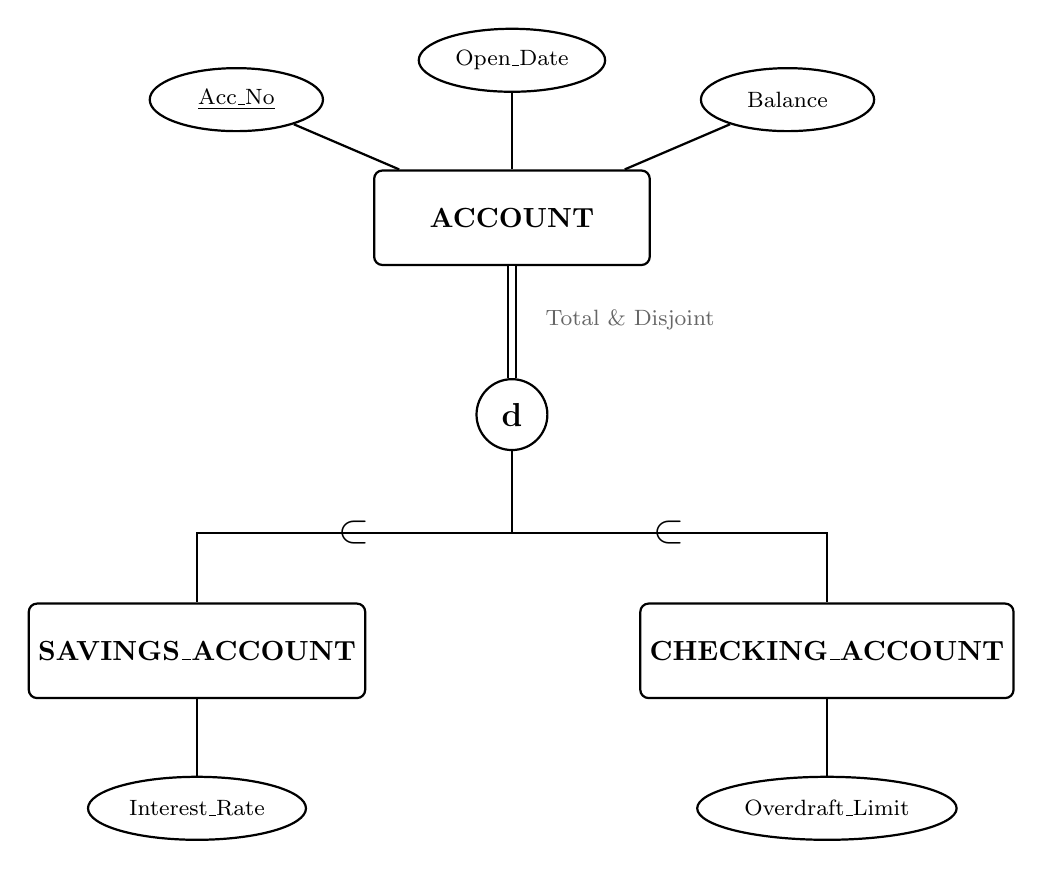
\begin{tikzpicture}[
    thick,
    entity/.style={draw, rectangle, rounded corners=3pt, minimum width=3.5cm, minimum height=1.2cm, align=center, fill=white, font=\bfseries},
    attribute/.style={draw, ellipse, minimum width=2.2cm, minimum height=0.8cm, align=center, fill=white, font=\footnotesize},
    d_node/.style={draw, circle, minimum size=0.9cm, align=center, fill=white, font=\bfseries\large}
]

    % ================= SUPERCLASS =================
    \node[entity] (ACC) at (0, 3) {ACCOUNT};
    
    % Superclass Attributes
    \node[attribute] (ano) at (-3.5, 4.5) {\underline{Acc\_No}};
    \node[attribute] (bal) at (3.5, 4.5) {Balance};
    \node[attribute] (odate) at (0, 5) {Open\_Date};
    
    \draw (ACC) -- (ano);
    \draw (ACC) -- (bal);
    \draw (ACC) -- (odate);

    % ================= DISJOINT NODE =================
    \node[d_node] (D) at (0, 0.5) {d};
    
    % Total Specialization (Double Line from Superclass to circle)
    \draw[double, double distance=2pt] (ACC) -- (D);
    \node[font=\footnotesize, text=gray!80!black] at (1.5, 1.7) {Total \& Disjoint};

    % ================= SUBCLASSES =================
    \node[entity] (SAV) at (-4, -2.5) {SAVINGS\_ACCOUNT};
    \node[entity] (CHK) at (4, -2.5) {CHECKING\_ACCOUNT};

    % Subclass Attributes
    \node[attribute] (irate) at (-4, -4.5) {Interest\_Rate};
    \draw (SAV) -- (irate);
    
    \node[attribute] (odlimit) at (4, -4.5) {Overdraft\_Limit};
    \draw (CHK) -- (odlimit);

    % ================= HIERARCHY CONNECTIONS =================
    % Orthogonal routing for clean EER structure
    \draw (D) -- (0, -1);
    \draw (0, -1) -| (SAV.north);
    \draw (0, -1) -| (CHK.north);

    % Subset symbols for Subclasses (Standard EER notation)
    \node[font=\Large] at (-2, -1) {$\subset$};
    \node[font=\Large] at (2, -1) {$\subset$};

\end{tikzpicture}
}
\end{center}
\vspace{0.5em}
\textbf{Note on the Diagram:} The double line from \textbf{ACCOUNT} to the \textbf{d} circle denotes \textit{total participation} (every account must be a specialized type). The \textbf{d} ensures \textit{disjointness} (an account cannot be both). The $\subset$ symbols denote the subset relationship (subclasses inherit from the superclass).

\end{tcolorbox}

\item YouTube is a very popular platform for hosting videos. People create channels and
upload videos on that. Sometimes the creators can batch up the videos into playlists.
Videos can be free to view or behind paywall which requires subscription to YouTube.
Premium. A free video can be watched with or without signing into YouTube. However,
only signed-in users' views are considered when counting the number of viewers for a
video. A signed-in account may or may not have corresponding channels. Each video has
a comment section where a signed-in user can comment; and comment to other people’s
comments. Also, videos contain some tags (given by the uploader or YouTube itself) that
help to filter videos. Signed-in users can subscribe to other channels. Now, for each of the
mentioned features below, design the corresponding portion of ERD for YouTube only.
Add attributes as you see fit and mark primary keys.
\begin{enumerate}
  \item \textbf{User management:} Users should be able to create accounts, create channels on top of
the accounts (one¢ user can create at most one channel), and subscribe to different
channels.
  \item \textbf{Video hosting:} Creators should be able to upload videos with different tags, and
create playlists by batching up multiple videos. Users should be able to view the videos,
find them in their history when needed and, also, check the number of viewers to the
videos.
  \item \textbf{Commenting:} Users should be able to comment on any video any number of times,
They should also be able to comment on other peoples comments.
  \item \textbf{Subscription system:} Creators should be able to mark some videos as premium (i.e.,
only subscribed users can view). Users should be able to buy subscriptions up to some
end date.

\item Implement relational schemas for each ERD you designed in this question.
\mk{15} \yr{CSE 215 | L-2/T-1 | 2022--23}
\end{enumerate}
\mk{20} \yr{CSE 215 | L-2/T-1 | 2022--23}

\begin{tcolorbox}[enhanced,breakable,ansbox,colback=cA!4,colframe=cA,boxrule=0.8pt,arc=5pt,title={\textbf{Answer}},fonttitle=\bfseries\color{white},colbacktitle=cA]

\section*{Entity-Relationship Diagrams (ERD) for YouTube Platform}

In this section, we decompose the platform's requirements into four distinct, logical ERD components to represent User Management, Video Hosting, Commenting, and Subscription mechanisms. Standard ERD notation is used: rectangles for entities, diamonds for relationships, ellipses for standard attributes, double ellipses for multivalued attributes, and dashed ellipses for derived attributes. 

\subsection*{1. User Management System}
\textbf{Working Principle:} A \textbf{User} can create an account and optionally create at most one \textbf{Channel}. Therefore, the \texttt{Owns} relationship is 1:1, with partial participation from the User (not all users create channels) and total participation from the Channel (every channel must be owned by a user). The \texttt{Subscribes\_To} relationship is M:N, as a user can subscribe to many channels, and a channel can have many subscribers.

\vspace{0.5cm}
\begin{center}
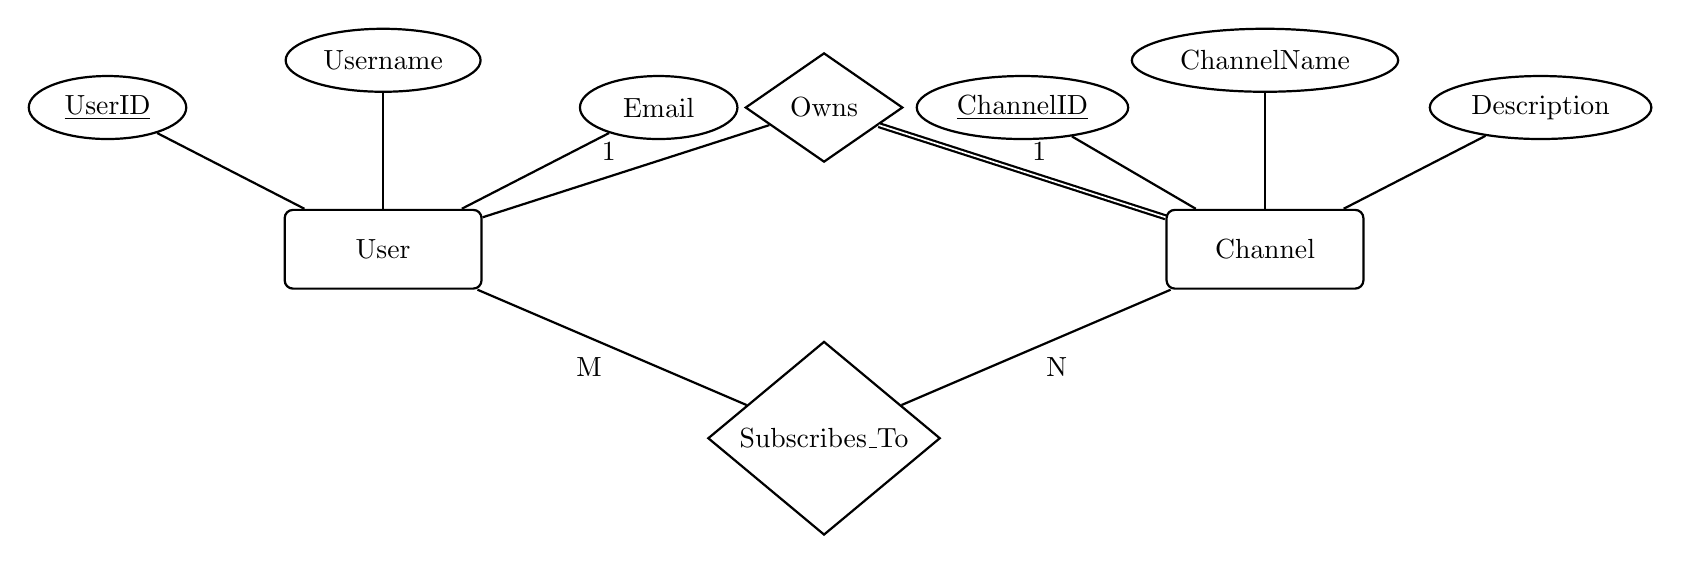
\begin{tikzpicture}[
x=1.4cm, thick,y=1.2cm, 
    entity/.style={rectangle, draw, thick, minimum width=2.5cm, minimum height=1cm, align=center, rounded corners=3pt},
    attribute/.style={ellipse, draw, thick, align=center, minimum width=2cm, minimum height=0.8cm},
    relationship/.style={diamond, draw, thick, aspect=1.2, align=center, minimum width=2cm, minimum height=1cm},
    line/.style={draw, thick}
]

    % Entities
    \node[entity] (user) at (0,0) {User};
    \node[entity] (channel) at (8,0) {Channel};

    % Attributes for User
    \node[attribute] (uid) at (-2.5, 1.5) {\underline{UserID}};
    \node[attribute] (uname) at (0, 2) {Username};
    \node[attribute] (uemail) at (2.5, 1.5) {Email};

    % Attributes for Channel
    \node[attribute] (cid) at (5.8, 1.5) {\underline{ChannelID}};
    \node[attribute] (cname) at (8, 2) {ChannelName};
    \node[attribute] (cdesc) at (10.5, 1.5) {Description};

    % Relationships
    \node[relationship] (owns) at (4, 1.5) {Owns};
    \node[relationship] (subs) at (4, -2) {Subscribes\_To};

    % Edges - Entity to Attribute
    \draw[line] (user) -- (uid);
    \draw[line] (user) -- (uname);
    \draw[line] (user) -- (uemail);
    
    \draw[line] (channel) -- (cid);
    \draw[line] (channel) -- (cname);
    \draw[line] (channel) -- (cdesc);

    % Edges - Entity to Relationship
    \draw[line] (user) -- (owns) node[midway, above left] {1};
    \draw[line, double] (owns) -- (channel) node[midway, above right] {1}; % Total participation
    
    \draw[line] (user) -- (subs) node[midway, below left] {M};
    \draw[line] (subs) -- (channel) node[midway, below right] {N};

\end{tikzpicture}
\end{center}

\vspace{1cm}
\subsection*{2. Video Hosting System}
\textbf{Working Principle:} The \textbf{Channel} entity uploads \textbf{Video} entities (1:N) and creates \textbf{Playlist} entities (1:N). Playlists can contain multiple videos, and videos can belong to multiple playlists (M:N). Signed-in \textbf{Users} watch videos, which is modeled by the M:N \texttt{Views} relationship. \texttt{Views} includes a \texttt{Timestamp} attribute to construct watch history. \texttt{Tags} is a multivalued attribute, while \texttt{ViewCount} is a derived attribute calculated from the \texttt{Views} relationship.

\vspace{0.5cm}
\begin{center}
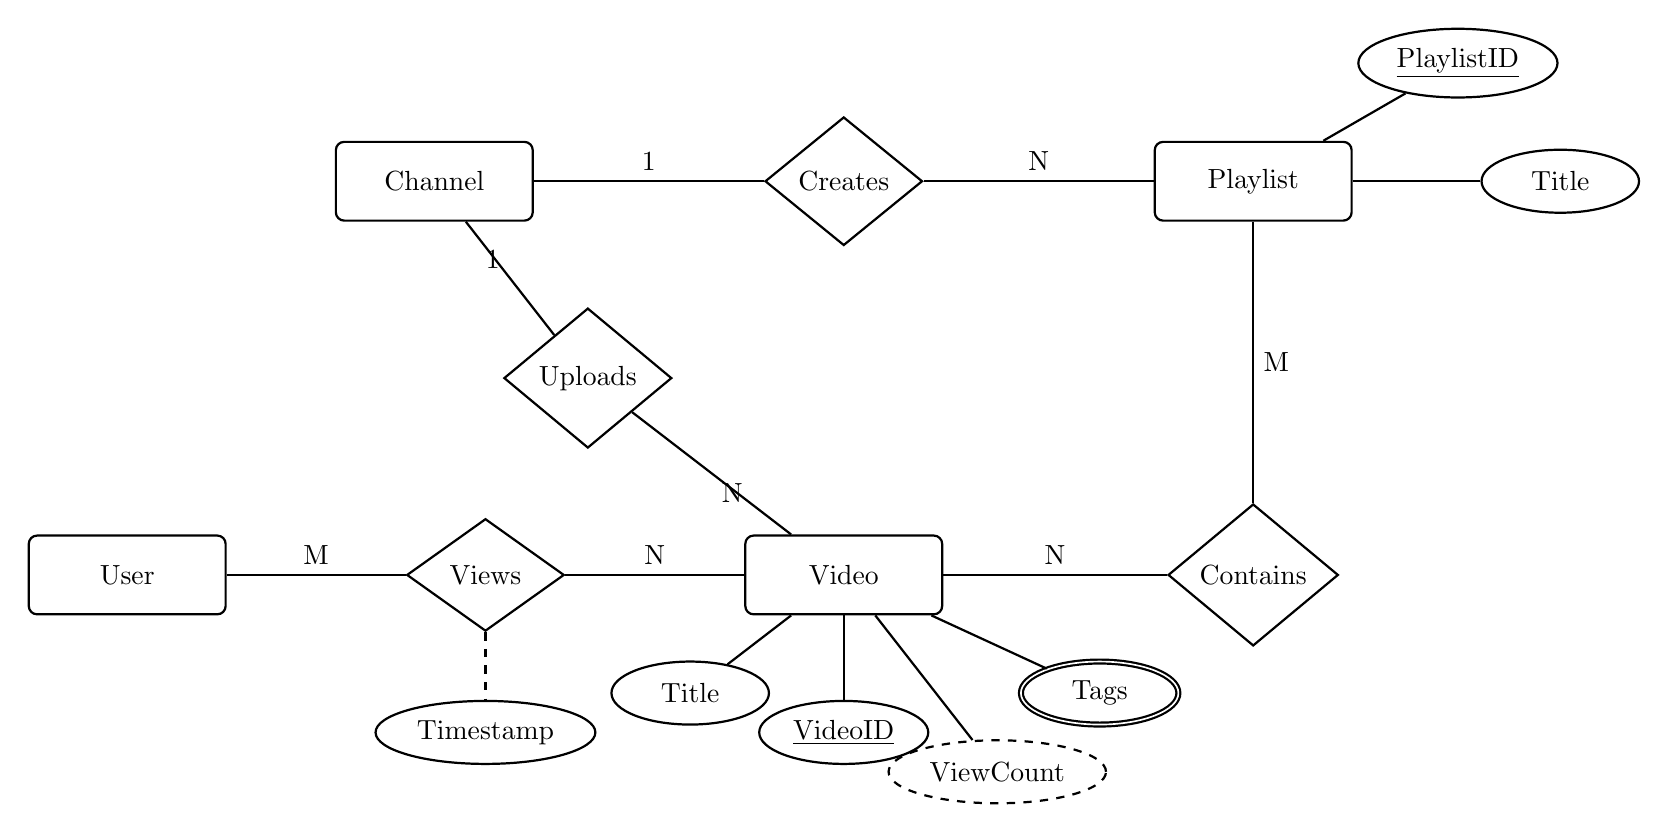
\begin{tikzpicture}[
    x=1.3cm, 
    entity/.style={rectangle, draw, thick, minimum width=2.5cm, minimum height=1cm, align=center, rounded corners=3pt},
    attribute/.style={ellipse, draw, thick, align=center, minimum width=2cm, minimum height=0.8cm},
    multiattribute/.style={ellipse, draw, thick, double, align=center, minimum width=2cm, minimum height=0.8cm},
    derivedattribute/.style={ellipse, draw, thick, dashed, align=center, minimum width=2cm, minimum height=0.8cm},
    relationship/.style={diamond, draw, thick, aspect=1.2, align=center, minimum width=2cm, minimum height=1cm},
    line/.style={draw, thick}
]

    % Entities
    \node[entity] (channel) at (0,6) {Channel};
    \node[entity] (playlist) at (8,6) {Playlist};
    \node[entity] (video) at (4,1) {Video};
    \node[entity] (user) at (-3,1) {User};

    % Relationships
    \node[relationship] (creates) at (4,6) {Creates};
    \node[relationship] (uploads) at (1.5, 3.5) {Uploads};
    \node[relationship] (contains) at (8, 1) {Contains};
    \node[relationship] (views) at (0.5, 1) {Views};

    % Attributes for Video
    \node[attribute] (vid) at (4, -1) {\underline{VideoID}};
    \node[attribute] (vtitle) at (2.5, -0.5) {Title};
    \node[multiattribute] (vtags) at (6.5, -0.5) {Tags};
    \node[derivedattribute] (vcount) at (5.5, -1.5) {ViewCount};
    
    % Attribute for Views relationship
    \node[attribute] (ts) at (0.5, -1) {Timestamp};

    % Attribute for Playlist
    \node[attribute] (pid) at (10, 7.5) {\underline{PlaylistID}};
    \node[attribute] (ptitle) at (11, 6) {Title};

    % Edges - Connections
    \draw[line] (channel) -- (creates) node[midway, above] {1};
    \draw[line] (creates) -- (playlist) node[midway, above] {N};
    
    \draw[line] (channel) -- (uploads) node[midway, above left] {1};
    \draw[line] (uploads) -- (video) node[midway, below right] {N};
    
    \draw[line] (playlist) -- (contains) node[midway, right] {M};
    \draw[line] (contains) -- (video) node[midway, above] {N};
    
    \draw[line] (user) -- (views) node[midway, above] {M};
    \draw[line] (views) -- (video) node[midway, above] {N};

    % Edges - Attributes
    \draw[line] (video) -- (vid);
    \draw[line] (video) -- (vtitle);
    \draw[line] (video) -- (vtags);
    \draw[line] (video) -- (vcount);
    
    \draw[line] (playlist) -- (pid);
    \draw[line] (playlist) -- (ptitle);
    
    \draw[line, dashed] (views) -- (ts);

\end{tikzpicture}
\end{center}

\vspace{1cm}
\subsection*{3. Commenting System}
\textbf{Working Principle:} A \textbf{Comment} is generated by a single \textbf{User} (1:N) and belongs to a specific \textbf{Video} (1:N). To facilitate comment threading and replies, we model a unary relationship \texttt{Replies\_To} on the \textbf{Comment} entity, establishing a recursive 1:N structural hierarchy where one parent comment can have multiple reply comments.

\vspace{0.5cm}
\begin{center}
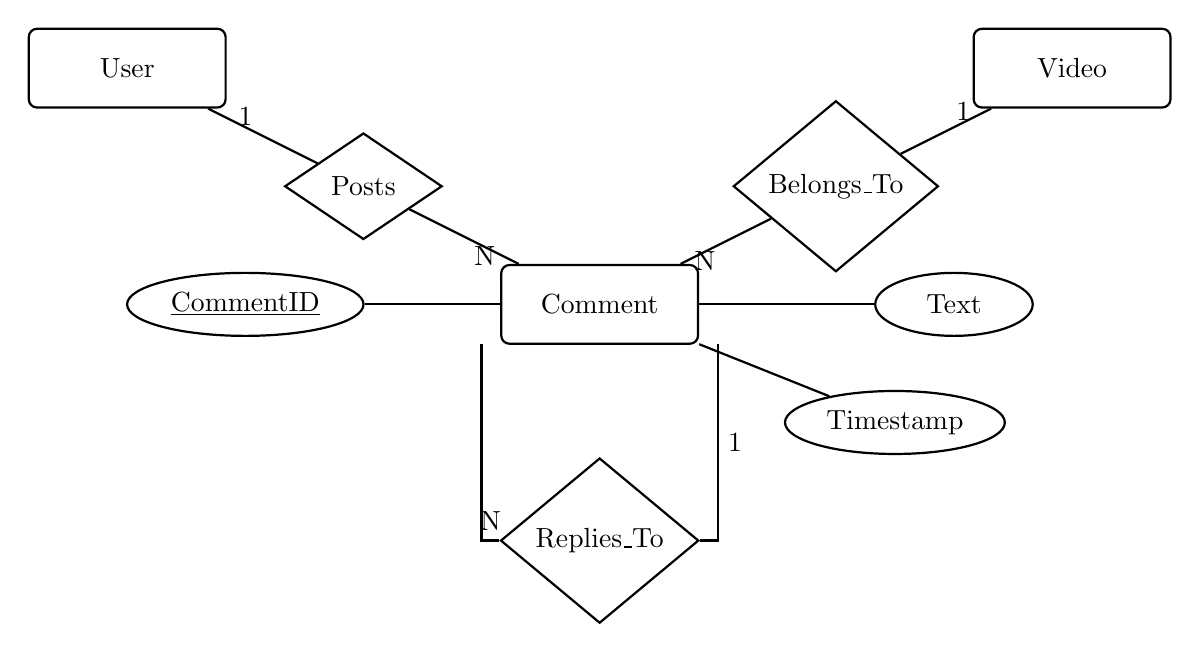
\begin{tikzpicture}[
x=1.5cm, thick , 
    entity/.style={rectangle, draw, thick, minimum width=2.5cm, minimum height=1cm, align=center, rounded corners=3pt},
    attribute/.style={ellipse, draw, thick, align=center, minimum width=2cm, minimum height=0.8cm},
    relationship/.style={diamond, draw, thick, aspect=1.2, align=center, minimum width=2cm, minimum height=1cm},
    line/.style={draw, thick}
]

    % Entities
    \node[entity] (user) at (-4,3) {User};
    \node[entity] (video) at (4,3) {Video};
    \node[entity] (comment) at (0,0) {Comment};

    % Relationships
    \node[relationship] (posts) at (-2,1.5) {Posts};
    \node[relationship] (belongsto) at (2,1.5) {Belongs\_To};
    \node[relationship] (replies) at (0,-3) {Replies\_To};

    % Comment Attributes
    \node[attribute] (cmid) at (-3, 0) {\underline{CommentID}};
    \node[attribute] (ctxt) at (3, 0) {Text};
    \node[attribute] (ctime) at (2.5, -1.5) {Timestamp};

    % Connect Entities and Relationships
    \draw[line] (user) -- (posts) node[midway, above left] {1};
    \draw[line] (posts) -- (comment) node[midway, below right] {N};
    
    \draw[line] (video) -- (belongsto) node[midway, above right] {1};
    \draw[line] (belongsto) -- (comment) node[midway, below left] {N};

    % Unary Relationship Loop
    \draw[line] (comment) +(-1,-0.5) -- (-1, -3) -- (replies) node[midway, above] {N};
    \draw[line] (replies) -- (1, -3) -- (1, -0.5) node[midway, right] {1};

    % Connect Attributes
    \draw[line] (comment) -- (cmid);
    \draw[line] (comment) -- (ctxt);
    \draw[line] (comment) -- (ctime);

\end{tikzpicture}
\end{center}

\vspace{1cm}
\subsection*{4. Subscription System}
\textbf{Working Principle:} A \textbf{User} can buy a \textbf{Subscription} to gain premium privileges (1:N relationship, as a user may renew or buy different tiered subscriptions over time). The premium status of a \textbf{Video} is encapsulated as a simple boolean attribute \texttt{IsPremium}. Only subscribed users are granted application-layer access to view videos marked with this flag.

\vspace{0.5cm}
\begin{center}
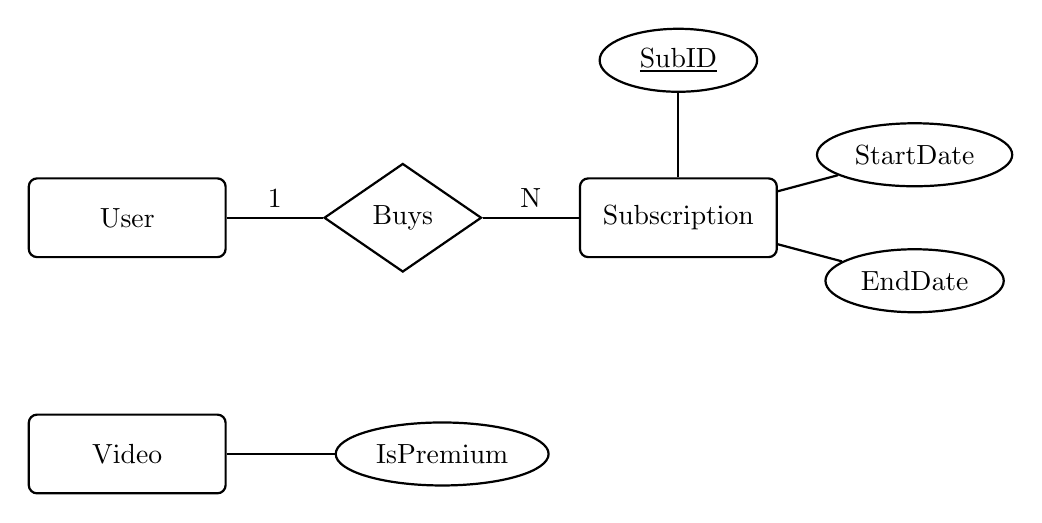
\begin{tikzpicture}[
    entity/.style={rectangle, draw, thick, minimum width=2.5cm, minimum height=1cm, align=center, rounded corners=3pt},
    attribute/.style={ellipse, draw, thick, align=center, minimum width=2cm, minimum height=0.8cm},
    relationship/.style={diamond, draw, thick, aspect=1.2, align=center, minimum width=2cm, minimum height=1cm},
    line/.style={draw, thick}
]

    % Entities
    \node[entity] (user) at (-3, 1) {User};
    \node[entity] (sub) at (4, 1) {Subscription};
    \node[entity] (video) at (-3, -2) {Video};

    % Relationships
    \node[relationship] (buys) at (0.5, 1) {Buys};

    % Attributes
    \node[attribute] (sid) at (4, 3) {\underline{SubID}};
    \node[attribute] (sdate) at (7, 1.8) {StartDate};
    \node[attribute] (edate) at (7, 0.2) {EndDate};
    
    \node[attribute] (isprem) at (1, -2) {IsPremium};

    % Lines
    \draw[line] (user) -- (buys) node[midway, above] {1};
    \draw[line] (buys) -- (sub) node[midway, above] {N};
    
    \draw[line] (sub) -- (sid);
    \draw[line] (sub) -- (sdate);
    \draw[line] (sub) -- (edate);
    
    \draw[line] (video) -- (isprem);

\end{tikzpicture}
\end{center}

\newpage
\subsection*{5. Relational Schemas}

Below is the complete relational schema mapping for the provided ERDs. Primary keys (PK) are strictly \underline{underlined}, and foreign keys (FK) refer to primary keys in their respective parent relations.

\vspace{0.5cm}
\begin{center}
\renewcommand{\arraystretch}{1.6}
\begin{tabular}{@{} >{\bfseries}l l l @{}}
\toprule
\textbf{Relation} & \textbf{Attributes (Primary Keys Underlined)} & \textbf{Foreign Keys (FK)} \\
\midrule

User & \underline{UserID}, Username, Email & None \\

Channel & \underline{ChannelID}, ChannelName, Description, UserID & UserID $\to$ User(UserID) \\

Subscribes & \underline{UserID}, \underline{ChannelID} & UserID $\to$ User, ChannelID $\to$ Channel \\

Playlist & \underline{PlaylistID}, Title, ChannelID & ChannelID $\to$ Channel(ChannelID) \\

Video & \underline{VideoID}, Title, IsPremium, ChannelID & ChannelID $\to$ Channel(ChannelID) \\

Video\_Tags & \underline{VideoID}, \underline{Tag} & VideoID $\to$ Video(VideoID) \\

Playlist\_Video & \underline{PlaylistID}, \underline{VideoID} & PlaylistID $\to$ Playlist, VideoID $\to$ Video \\

Viewing\_History & \underline{UserID}, \underline{VideoID}, \underline{Timestamp} & UserID $\to$ User, VideoID $\to$ Video \\

Comment & \underline{CommentID}, Text, Timestamp, UserID, VideoID, ParentID & \begin{tabular}{@{}l@{}}UserID $\to$ User(UserID) \\ VideoID $\to$ Video(VideoID) \\ ParentID $\to$ Comment(CommentID)\end{tabular} \\

Subscription & \underline{SubID}, StartDate, EndDate, UserID & UserID $\to$ User(UserID) \\

\bottomrule
\end{tabular}
\end{center}

\vspace{0.5cm}
\subsubsection*{Key Mapping Decisions \& Notes}
\begin{itemize}
    \item \textbf{1:1 Relationship (Owns):} The 1:1 relationship between \texttt{User} and \texttt{Channel} is mapped by placing \texttt{UserID} as a foreign key in the \texttt{Channel} relation (as a user might not have a channel, but every channel must have a user, ensuring no nulls).
    \item \textbf{M:N Relationships:} \texttt{Subscribes}, \texttt{Playlist\_Video}, and \texttt{Viewing\_History} are intersection tables created from the many-to-many ERD relationships.
    \item \textbf{Multivalued Attribute:} The \texttt{Tags} attribute is extracted into its own table \texttt{Video\_Tags} with a composite primary key.
    \item \textbf{Unary Relationship (Replies\_To):} Modeled via \texttt{ParentID} within the \texttt{Comment} table, referencing the same table's \texttt{CommentID}. It is nullable to allow top-level comments.
    \item \textbf{Derived Attribute:} \texttt{ViewCount} is omitted from the base schema as it is dynamically computed using a \texttt{COUNT()} aggregate function query on the \texttt{Viewing\_History} table.
\end{itemize}

\end{tcolorbox}


\item Give an example of a Non-Binary Relationship. What issues arise for Non-Binary Relationships?
\mk{5} \yr{CSE 215 | L-2/T-1 | 2022--23}

\begin{tcolorbox}[enhanced,breakable,ansbox,colback=cA!4,colframe=cA,boxrule=0.8pt,arc=5pt,title={\textbf{Answer}},fonttitle=\bfseries\color{white},colbacktitle=cA]

\subsection*{1. Non-Binary Relationship: Definition and Example}

\subsubsection*{Definition}
A \textbf{non-binary relationship} (also known as an $n$-ary relationship) is a relationship in an Entity-Relationship (ER) model that connects \textbf{three or more} entity sets simultaneously. Unlike a binary relationship, which relates exactly two entities, an $n$-ary relationship represents an atomic association among a combination of entities that cannot be naturally separated without losing contextual semantics. The most common form of a non-binary relationship is a \textbf{ternary relationship} ($n=3$).

\subsubsection*{Real-World Example}
Consider a manufacturing and supply chain system consisting of three entity sets:
\begin{itemize}
    \item \textbf{Supplier}: The vendor providing components.
    \item \textbf{Part}: The specific item or component being supplied.
    \item \textbf{Project}: The construction project or department utilizing the parts.
\end{itemize}
A binary relationship between \textbf{Supplier} and \textbf{Part} would only indicate what parts a supplier can provide. A binary relationship between \textbf{Supplier} and \textbf{Project} would only specify which suppliers serve which projects. 

However, to record that \textit{"Supplier $S_1$ supplies Part $P_1$ to Project $J_1$"} requires a \textbf{ternary relationship} named \textbf{Supplies}. This association is atomic because a supplier might supply a part to one specific project, but not to another.

\subsubsection*{Ternary Relationship Diagram (TikZ)}

\begin{center}
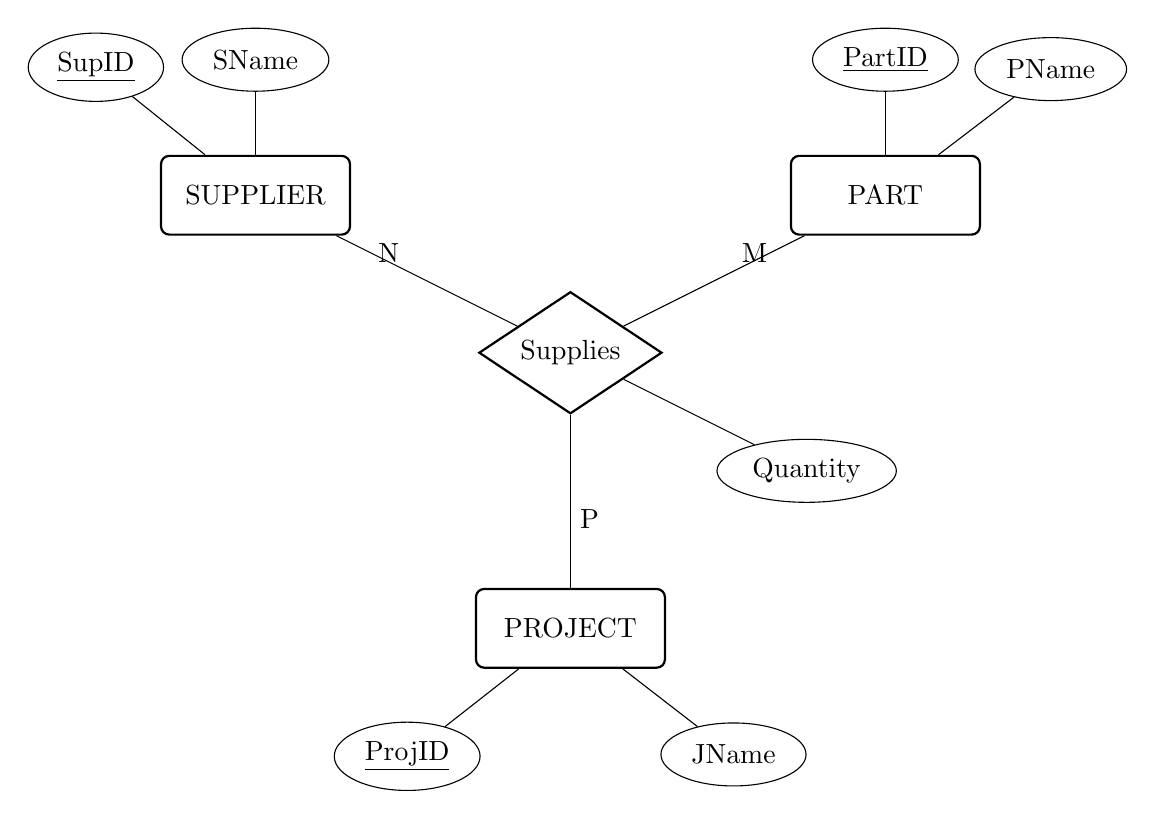
\begin{tikzpicture}[node distance=4cm, every edge/.style={link},
    entity/.style={rectangle, draw, black, thick, minimum width=2.4cm, minimum height=1cm, rounded corners=3pt, align=center},
    relationship/.style={diamond, draw, black, thick, minimum width=2cm, minimum height=1.2cm, aspect=1.5, align=center},
    attribute/.style={ellipse, draw, black, thin, minimum width=1.6cm, minimum height=0.8cm, align=center},
    link/.style={draw, black, thick}]

    % Central Ternary Relationship
    \node[relationship] (supplies) at (0,0) {Supplies};

    % Entities arranged symmetrically around the central diamond
    \node[entity] (supplier) at (-4, 2) {SUPPLIER};
    \node[entity] (part) at (4, 2) {PART};
    \node[entity] (project) at (0, -3.5) {PROJECT};

    % Descriptive attribute attached directly to the relationship
    \node[attribute] (quantity) at (3, -1.5) {Quantity};

    % Attributes for SUPPLIER
    \node[attribute] (s_id) [above left=0.8cm and 0.2cm of supplier] {\underline{SupID}};
    \node[attribute] (s_name) [above=0.8cm of supplier] {SName};

    % Attributes for PART
    \node[attribute] (p_id) [above=0.8cm of part] {\underline{PartID}};
    \node[attribute] (p_name) [above right=0.8cm and 0.2cm of part] {PName};

    % Attributes for PROJECT
    \node[attribute] (j_id) [below left=0.8cm and 0.2cm of project] {\underline{ProjID}};
    \node[attribute] (j_name) [below right=0.8cm and 0.2cm of project] {JName};

    % Connecting attributes to entities
    \draw (supplier) -- (s_id);
    \draw (supplier) -- (s_name);
    \draw (part) -- (p_id);
    \draw (part) -- (p_name);
    \draw (project) -- (j_id);
    \draw (project) -- (j_name);

    % Connecting entities to relationship
    \draw (supplier) -- (supplies) node[pos=0.4, above left] {N};
    \draw (part) -- (supplies) node[pos=0.4, above right] {M};
    \draw (project) -- (supplies) node[pos=0.4, right] {P};
    
    % Connecting descriptive attribute to relationship
    \draw (supplies) -- (quantity);

\end{tikzpicture}
\end{center}

---

\subsection*{2. Issues and Challenges in Non-Binary Relationships}

Designers face several structural, semantic, and performance complications when dealing with non-binary relationships:

\begin{enumerate}
    \item \textbf{Ambiguity in Cardinality Constraints}
    \begin{itemize}
        \item In a binary relationship, structural constraints (1:1, 1:N, M:N) have clear and standardized meanings. In an $n$-ary relationship, the interpretation of cardinalities becomes ambiguous and varies across design methodologies (e.g., Chen notation vs. Barker notation).
        \item For instance, a directed arrow or a "$1$" pointing from \textbf{Project} to the \textbf{Supplies} relationship can mean two completely different things depending on the conventions chosen:
        \begin{itemize}
            \item \textit{Interpretation A:} For a given combination of a Supplier and a Part, there is at most one unique Project.
            \item \textit{Interpretation B:} A single Project is constrained to only ever receive one unique combination of Part and Supplier.
        \end{itemize}
    \end{itemize}

    \item \textbf{False Decomposition Traps (Loss of Semantics)}
    \begin{itemize}
        \item Database designers often attempt to simplify their schema by splitting a ternary relationship into three distinct binary relationships: (\texttt{Supplier-Part}), (\texttt{Part-Project}), and (\texttt{Supplier-Project}).
        \item This often introduces a semantic flaw known as a \textbf{connection trap} or \textbf{fan trap}. Knowing that Supplier $A$ makes Part $X$, Part $X$ is used in Project $Y$, and Supplier $A$ works on Project $Y$ does \textit{not} guarantee that Supplier $A$ supplies Part $X$ specifically \textit{to} Project $Y$. The exact instance mapping is completely lost.
    \end{itemize}

    \item \textbf{Over-Structuring / Redundancy}
    \begin{itemize}
        \item Conversely, using an $n$-ary relationship when separate binary relationships are sufficient introduces unnecessary constraints and data redundancies. For example, if a supplier always supplies a part to every project uniformly, treating this as an atomic ternary entity artificially pairs instances that do not depend on one another.
    \end{itemize}

    \item \textbf{Logical Representation and Null Value Pitfalls}
    \begin{itemize}
        \item In a true ternary relationship, all participating entity instances must exist simultaneously to form a valid relationship tuple. 
        \item If a supplier introduces a new part that has not yet been assigned to any project, this instance cannot be inserted into the ternary relation without introducing a \texttt{NULL} value for the \texttt{ProjID} attribute, which violates the integrity rules if \texttt{ProjID} forms part of the primary key.
    \end{itemize}

    \item \textbf{Physical Performance and Optimization Issues}
    \begin{itemize}
        \item When converted into relational schemas, $n$-ary tables require composite primary keys composed of the primary keys of all participating entities: $\text{PK} = \{\text{SupID}, \text{PartID}, \text{ProjID}\}$.
        \item Queries tracking down basic relationships often degrade into expensive multi-way join operations across massive junction tables, leading to storage layout overhead and indexing complexities.
    \end{itemize}
\end{enumerate}

\subsubsection*{Comparison: Binary Decomposition vs. Ternary Representation}

\begin{center}
\begin{tabular}{lll}
\toprule
\textbf{Property} & \textbf{Decomposed Binary Setup} & \textbf{True Ternary Setup} \\
\midrule
\textbf{Structural Complexity} & Low (Simple 2-entity links) & High ($n$-way connection mapping) \\
\textbf{Semantic Precision} & Prone to connection traps & Completely accurate atomic tracking \\
\textbf{Primary Key Composition} & Simple keys & Large composite foreign keys \\
\textbf{Instance Independence} & Entities can pair independently & All $n$ entities must coexist in the tuple \\
\bottomrule
\end{tabular}
\end{center}

\end{tcolorbox}

\item Suppose you are given the following requirements for a simple database for the Bangladesh Premier League (BPL) in a season:
\begin{itemize}[leftmargin=1.5em,itemsep=1pt]
  \item The BPL has many teams; each team has a name, a city, a coach, a captain, and a set of players.
  \item Each player belongs to only one team; a player may not be hired by any team.
  \item Each player has a name, a fielding position (such as slip, mid-wicket, long on, long off etc), a ranking, and a set of injury records.
  \item A team captain is also a player.
  \item Injury records must have an id, period (start and end), and a short description.
  \item A game is played between two teams (host\_team and guest\_team) with a date (such as May 11th, 2023) and scores (winning and losing team scores such as 143/10 and 148/6).
\end{itemize}
Construct a clean and concise E/R diagram for the BPL database. List your assumptions and clearly indicate cardinality mappings and any role indicators.
\mk{10} \yr{CSE 215 | L-2/T-2 | 2021--22}

\begin{tcolorbox}[enhanced,breakable,ansbox,colback=cA!4,colframe=cA,boxrule=0.8pt,arc=5pt,title={\textbf{Answer}},fonttitle=\bfseries\color{white},colbacktitle=cA]

\subsection*{1. Design Assumptions}
To establish exact operational boundaries and clear cardinality mapping within the Entity-Relationship (ER) model, the following domain-specific design assumptions are made based on the provided requirements:
\begin{itemize}
    \item \textbf{Team \& Captaincy:} A team has exactly one captain at any time. The captain must be an active player on that team. This is modeled via a $1:1$ relationship with a role indicator (\textbf{Captain}).
    \item \textbf{Player Assignment:} Each player belongs to \textbf{at most one} team. The constraint "a player may not be hired by any team" indicates partial participation ($0:1$) from the \textbf{PLAYER} side.
    \item \textbf{Injury Records:} Injury records cannot exist independently of a player. Thus, \textbf{INJURY\_RECORD} is modeled as a \textbf{weak entity} set structurally dependent on the \textbf{PLAYER} entity set via an identifying relationship. Its unique descriptor within a player is an partial key (\texttt{InjuryID}).
    \item \textbf{Game Scheduling:} A game represents a head-to-head match between exactly two distinct teams: a \textbf{Host Team} and a \textbf{Guest Team}. It is modeled as a binary relationship between \textbf{TEAM} and itself (a recursive/unary relationship) with distinct role indicators, capturing the date and performance statistics (scores).
\end{itemize}

\subsection*{2. Entity-Relationship Diagram}

\begin{center}
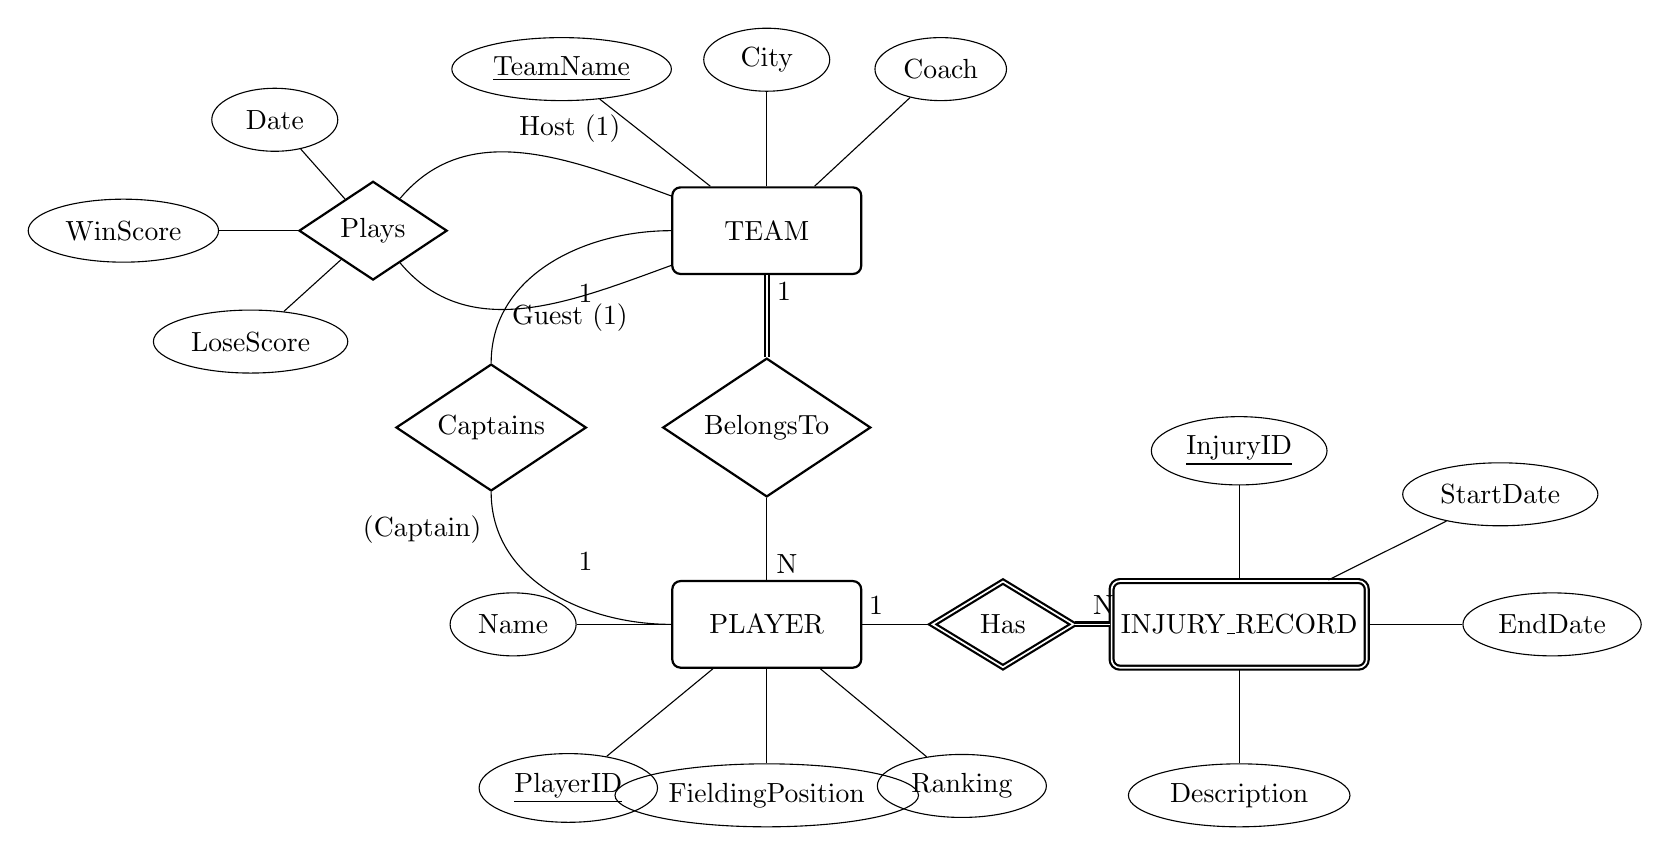
\begin{tikzpicture}[node distance=3.5cm,
    entity/.style={rectangle, draw, black, thick, minimum width=2.4cm, minimum height=1.1cm, rounded corners=3pt, align=center},
    weak_entity/.style={rectangle, draw, black, thick, double, minimum width=2.4cm, minimum height=1.1cm, rounded corners=3pt, align=center},
    relationship/.style={diamond, draw, black, thick, minimum width=1.8cm, minimum height=1.1cm, aspect=1.5, align=center},
    weak_relationship/.style={diamond, draw, black, thick, double, minimum width=1.8cm, minimum height=1.1cm, aspect=1.5, align=center},
    attribute/.style={ellipse, draw, black, thin, minimum width=1.6cm, minimum height=0.8cm, align=center},
    link/.style={draw, black, thick}]

    % --- Layout Nodes Placement ---
    \node[entity] (team) at (0,4) {TEAM};
    \node[entity] (player) at (0,-1) {PLAYER};
    \node[weak_entity] (injury) at (6,-1) {INJURY\_RECORD};

    % --- TEAM Attributes ---
    \node[attribute] (t_name) [above left=1.2cm and 0.4cm of team] {\underline{TeamName}};
    \node[attribute] (t_city) [above=1.2cm of team] {City};
    \node[attribute] (t_coach) [above right=1.2cm and 0.4cm of team] {Coach};
    \draw (team) -- (t_name);
    \draw (team) -- (t_city);
    \draw (team) -- (t_coach);

    % --- PLAYER Attributes ---
    \node[attribute] (p_id) [below left=1.2cm and 0.5cm of player] {\underline{PlayerID}};
    \node[attribute] (p_name) [left=1.2cm of player] {Name};
    \node[attribute] (p_pos) [below=1.2cm of player] {FieldingPosition};
    \node[attribute] (p_rank) [below right=1.2cm and 0.5cm of player] {Ranking};
    \draw (player) -- (p_id);
    \draw (player) -- (p_name);
    \draw (player) -- (p_pos);
    \draw (player) -- (p_rank);

    % --- INJURY_RECORD Attributes ---
    \node[attribute] (i_id) [above=1.2cm of injury] {\underline{InjuryID}};
    \node[attribute] (i_start) [above right=0.8cm and 0.8cm of injury] {StartDate};
    \node[attribute] (i_end) [right=1.2cm of injury] {EndDate};
    \node[attribute] (i_desc) [below=1.2cm of injury] {Description};
    \draw (injury) -- (i_id);
    \draw (injury) -- (i_start);
    \draw (injury) -- (i_end);
    \draw (injury) -- (i_desc);

    % --- Relationships ---

    % 1. TEAM - PLAYER (BelongsTo)
    \node[relationship] (belongs) at (0,1.5) {BelongsTo};
    \draw[double, thick] (team) -- (belongs) node[pos=0.2, right] {1};
    \draw (player) -- (belongs) node[pos=0.2, right] {N};

    % 2. TEAM - PLAYER (Captains)
    \node[relationship] (captains) at (-3.5,1.5) {Captains};
    \draw (team) to[out=180, in=90] (captains);
    \draw (captains) to[out=270, in=180] (player);
    \node at (-2.3, 3.2) {1};
    \node at (-2.3, -0.2) {1};
    \node at (-3.5, 0.2) [left] {(Captain)};

    % 3. PLAYER - INJURY_RECORD (HasInjury) - Identifying
    \node[weak_relationship] (has_injury) at (3,-1) {Has};
    \draw (player) -- (has_injury) node[pos=0.2, above] {1};
    \draw[double, thick] (injury) -- (has_injury) node[pos=0.2, above] {N};

    % 4. TEAM - TEAM Unary/Recursive (Plays)
    \node[relationship] (plays) at (-5,4) {Plays};
    \draw (team) to[out=160, in=50] (plays);
    \draw (plays) to[out=310, in=200] (team);
    \node at (-2.5, 5.0) [above] {Host (1)};
    \node at (-2.5, 3.2) [below] {Guest (1)};
    
    % Plays Attributes
    \node[attribute] (g_date) [above left=0.8cm and 0.2cm of plays] {Date};
    \node[attribute] (g_win) [left=1.0cm of plays] {WinScore};
    \node[attribute] (g_lose) [below left=0.8cm and 0.2cm of plays] {LoseScore};
    \draw (plays) -- (g_date);
    \draw (plays) -- (g_win);
    \draw (plays) -- (g_lose);

\end{tikzpicture}
\end{center}

\subsection*{3. Schema Map Summary}

\begin{center}
\begin{tabular}{llccp{7cm}}
\toprule
\textbf{Relation/Link} & \textbf{Type} & \textbf{Participation (Team)} & \textbf{Participation (Player)} & \textbf{Structural Meaning} \\
\midrule
\texttt{BelongsTo} & Binary & Total ($1$) & Partial ($N$) & A player is restricted to at most one team; a team possesses many players. \\
\texttt{Captains} & Binary & Partial ($1$) & Partial ($1$) & One specific player manages a specific team as a captain. \\
\texttt{Plays} & Unary & Partial ($1$) & --- & Connects a host team and guest team together for an individual fixture. \\
\texttt{Has} & Weak & --- & Total ($1$) & Structural dependency linking players tightly to their history of ailments. \\
\bottomrule
\end{tabular}
\end{center}

\end{tcolorbox}

\item Consider the following descriptions of an organization having many EMPLOYEES.

\begin{enumerate}[label=(\roman*)]
    \item An EMPLOYEE has a name, nid number, data of birth, and address.
    \item Based on the EMPLOYEE's Job, EMPLOYEE may be further grouped into:\\
    SECRETARY, ENGINEER, TECHNICIAN, and MANAGER
    \item Based on the EMPLOYEE's method of pay, EMPLOYEE may also be grouped into:\\
    SALARIED\_EMPLOYEE, and HOURLY\_EMPLOYEE
    \item A salaried employee who is also an engineer belongs to the two subclasses:\\
    ENGINEER, and SALARIED\_EMPLOYEE
    \item A salaried employee who is also an engineering manager belongs to the three subclasses:\\
    MANAGER, ENGINEER, and SALARIED\_EMPLOYEE.
    \item We want to record typing speed of each SECRETARY.
    \item Each technician has a technical grade ( a number) which depends on his skill level
    \item Each Engineer has a type (ME, CSE, EEE, etc \dots)
    \item Each MANAGER manages at least one project, each project has a project id, title, and a project value.
    \item Each HOURLY\_EMPLOYEE is a member of some TRADE\_UNION which has a name and member count.
\end{enumerate}

\begin{itemize}
    \item Construct an E/R diagram with the above description; clearly indicate the cardinality mappings as well as any role indicators in your E/R diagram.
    \item Convert the E/R diagram into a set of relational database schema. You should avoid keeping null values in attributes.
\end{itemize}
\mk{20} \yr{CSE 215 | L-2/T-2 | 2021--22}

\begin{tcolorbox}[enhanced,breakable,ansbox,colback=cA!4,colframe=cA,boxrule=0.8pt,arc=5pt,title={\textbf{Answer}},fonttitle=\bfseries\color{white},colbacktitle=cA]

\section*{Part (i): Enhanced Entity-Relationship (EER) Diagram}

\textbf{Design Principles \& Generalization Modeling:}
\begin{itemize}
    \item \textbf{Superclass:} \textbf{EMPLOYEE} acts as the root entity containing shared attributes (\texttt{NID}, \texttt{Name}, \texttt{DOB}, \texttt{Address}).
    \item \textbf{Generalization 1 (Pay Method):} Disjoint (\textbf{d}) specialization because an employee is either a \textbf{SALARIED\_EMPLOYEE} or an \textbf{HOURLY\_EMPLOYEE}, but not both.
    \item \textbf{Generalization 2 (Job Role):} Overlapping (\textbf{o}) specialization because an employee can simultaneously hold multiple roles (e.g., an \textbf{ENGINEER} who is also a \textbf{MANAGER}). 
    \item \textbf{Relationships:} The \textbf{MANAGER} explicitly participates totally in the \texttt{Manages} relationship with \textbf{PROJECT} (1:N assumption). Similarly, \textbf{HOURLY\_EMPLOYEE} totally participates in the \texttt{Member\_Of} relationship with \textbf{TRADE\_UNION} (N:1 assumption).
\end{itemize}

\vspace{0.5cm}



\begin{center}
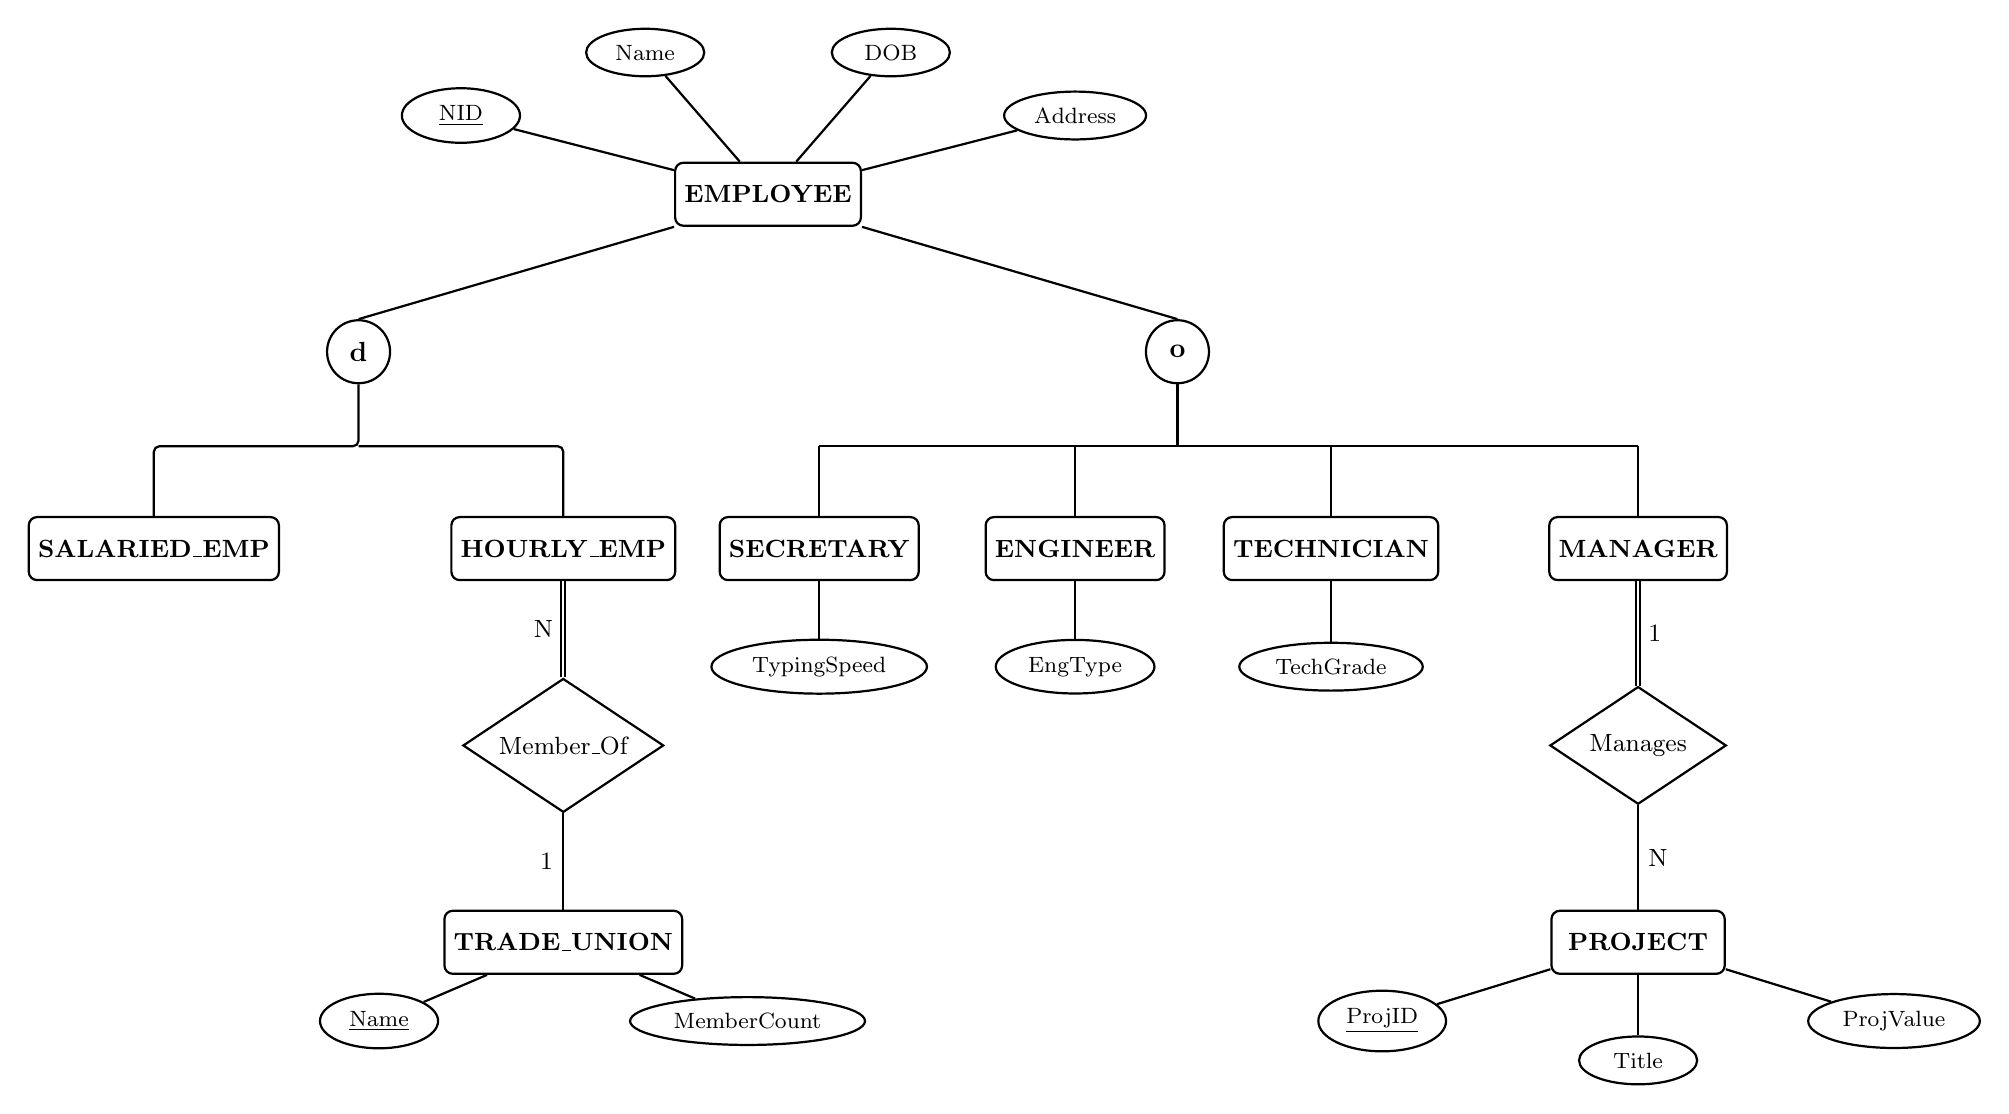
\begin{tikzpicture}[
x=1.3cm,
    entity/.style={rectangle, draw, thick, minimum width=2.2cm, minimum height=0.8cm, align=center, rounded corners=3pt, font=\small\bfseries},
    attribute/.style={ellipse, draw, thick, align=center, minimum width=1.5cm, minimum height=0.6cm, font=\footnotesize},
    relationship/.style={diamond, draw, thick, aspect=1.5, align=center, minimum width=2cm, minimum height=0.8cm, font=\small},
    isa/.style={circle, draw, thick, align=center, minimum size=0.8cm, font=\bfseries},
    line/.style={draw, thick},
    ortho/.style={draw, thick, rounded corners=2pt}
]

    % --- Root Entity ---
    \node[entity] (emp) at (0, 0) {EMPLOYEE};
    
    % Attributes of EMPLOYEE
    \node[attribute] (nid) at (-3, 1) {\underline{NID}};
    \node[attribute] (name) at (-1.2, 1.8) {Name};
    \node[attribute] (dob) at (1.2, 1.8) {DOB};
    \node[attribute] (addr) at (3, 1) {Address};
    
    \draw[line] (emp) -- (nid);
    \draw[line] (emp) -- (name);
    \draw[line] (emp) -- (dob);
    \draw[line] (emp) -- (addr);

    % --- Specialization Categories ---
    \node[isa] (isapay) at (-4, -2) {d};
    \node[isa] (isajob) at (4, -2) {o};
    
    \draw[line] (emp.south west) -- (isapay.north);
    \draw[line] (emp.south east) -- (isajob.north);
    
    % -- Pay Specialization Subclasses --
    \node[entity] (salaried) at (-6, -4.5) {SALARIED\_EMP};
    \node[entity] (hourly) at (-2, -4.5) {HOURLY\_EMP};
    
    % Routing lines for disjoint (Pay)
    \draw[ortho] (isapay.south) -- (-4, -3.2) -- (-6, -3.2) -- (salaried.north);
    \draw[ortho] (-4, -3.2) -- (-2, -3.2) -- (hourly.north);
    
    % -- Job Specialization Subclasses --
    \node[entity] (sec) at (0.5, -4.5) {SECRETARY};
    \node[entity] (eng) at (3, -4.5) {ENGINEER};
    \node[entity] (tech) at (5.5, -4.5) {TECHNICIAN};
    \node[entity] (mgr) at (8.5, -4.5) {MANAGER};
    
    % Routing lines for overlapping (Job)
    \draw[line] (isajob.south) -- (4, -3.2);
    \draw[ortho] (0.5, -3.2) -- (8.5, -3.2);
    \draw[line] (0.5, -3.2) -- (sec.north);
    \draw[line] (3, -3.2) -- (eng.north);
    \draw[line] (5.5, -3.2) -- (tech.north);
    \draw[line] (8.5, -3.2) -- (mgr.north);

    % -- Subclass Attributes --
    \node[attribute] (tspeed) at (0.5, -6) {TypingSpeed};
    \draw[line] (sec) -- (tspeed);
    
    \node[attribute] (etype) at (3, -6) {EngType};
    \draw[line] (eng) -- (etype);
    
    \node[attribute] (tgrade) at (5.5, -6) {TechGrade};
    \draw[line] (tech) -- (tgrade);

    % --- Additional Entities and Relationships ---
    
    % Hourly Employee to Trade Union
    \node[relationship] (member) at (-2, -7) {Member\_Of};
    \node[entity] (union) at (-2, -9.5) {TRADE\_UNION};
    
    \node[attribute] (uname) at (-3.8, -10.5) {\underline{Name}};
    \node[attribute] (ucount) at (-0.2, -10.5) {MemberCount};
    
    \draw[line, double] (hourly) -- (member) node[midway, left, font=\small] {N};
    \draw[line] (member) -- (union) node[midway, left, font=\small] {1};
    \draw[line] (union) -- (uname);
    \draw[line] (union) -- (ucount);
    
    % Manager to Project
    \node[relationship] (manages) at (8.5, -7) {Manages};
    \node[entity] (proj) at (8.5, -9.5) {PROJECT};
    
    \node[attribute] (pid) at (6, -10.5) {\underline{ProjID}};
    \node[attribute] (ptitle) at (8.5, -11) {Title};
    \node[attribute] (pval) at (11, -10.5) {ProjValue};
    
    % Double line indicates "each manager manages at least one project" (Total Participation)
    \draw[line, double] (mgr) -- (manages) node[midway, right, font=\small] {1};
    \draw[line] (manages) -- (proj) node[midway, right, font=\small] {N};
    
    \draw[line] (proj) -- (pid);
    \draw[line] (proj) -- (ptitle);
    \draw[line] (proj) -- (pval);

\end{tikzpicture}
\end{center}

\vspace{1cm}

\section*{Part (ii): Relational Schema Mapping}

To \textbf{avoid null values}, we use the approach where multiple relations are created (one for the superclass and one for each subclass). Subclass tables only contain their specific attributes and the primary key of the superclass.

\begin{center}
\renewcommand{\arraystretch}{1.5}
\begin{tabular}{@{} >{\bfseries}l l l @{}}
\toprule
\textbf{Relation} & \textbf{Attributes (Primary Keys Underlined)} & \textbf{Foreign Keys (FK)} \\
\midrule
EMPLOYEE & \underline{NID}, Name, DOB, Address & None \\

SALARIED\_EMP & \underline{NID} & NID $\to$ EMPLOYEE(NID) \\

TRADE\_UNION & \underline{Name}, MemberCount & None \\

HOURLY\_EMP & \underline{NID}, UnionName & 
    \begin{tabular}{@{}l@{}}
        NID $\to$ EMPLOYEE(NID) \\
        UnionName $\to$ TRADE\_UNION(Name)
    \end{tabular} \\

SECRETARY & \underline{NID}, TypingSpeed & NID $\to$ EMPLOYEE(NID) \\

ENGINEER & \underline{NID}, EngType & NID $\to$ EMPLOYEE(NID) \\

TECHNICIAN & \underline{NID}, TechGrade & NID $\to$ EMPLOYEE(NID) \\

MANAGER & \underline{NID} & NID $\to$ EMPLOYEE(NID) \\

PROJECT & \underline{ProjID}, Title, ProjValue, ManagerNID & ManagerNID $\to$ MANAGER(NID) \\
\bottomrule
\end{tabular}
\end{center}

\subsubsection*{Design Notes on the Transformation:}
\begin{enumerate}
    \item \textbf{Generalization:} Subclasses inherit the primary key (\texttt{NID}) from \texttt{EMPLOYEE}. Since a single employee can be an engineer and a manager, their \texttt{NID} will simply appear in both the \texttt{ENGINEER} and \texttt{MANAGER} tables without issue. No \texttt{NULL} values are generated for attributes that don't apply to specific roles.
    \item \textbf{1:N Relationship (Manages):} The 1:N relationship between \textbf{MANAGER} and \textbf{PROJECT} is handled by placing the manager's primary key (\texttt{ManagerNID}) into the \texttt{PROJECT} table as a foreign key.
    \item \textbf{N:1 Relationship (Member\_Of):} The relationship between \textbf{HOURLY\_EMPLOYEE} and \textbf{TRADE\_UNION} is handled by placing the union's primary key (\texttt{UnionName}) into the \texttt{HOURLY\_EMP} table.
\end{enumerate}

\end{tcolorbox}


\item Convert the E/R diagram of Figure below into a relational database schema.

\begin{center}
  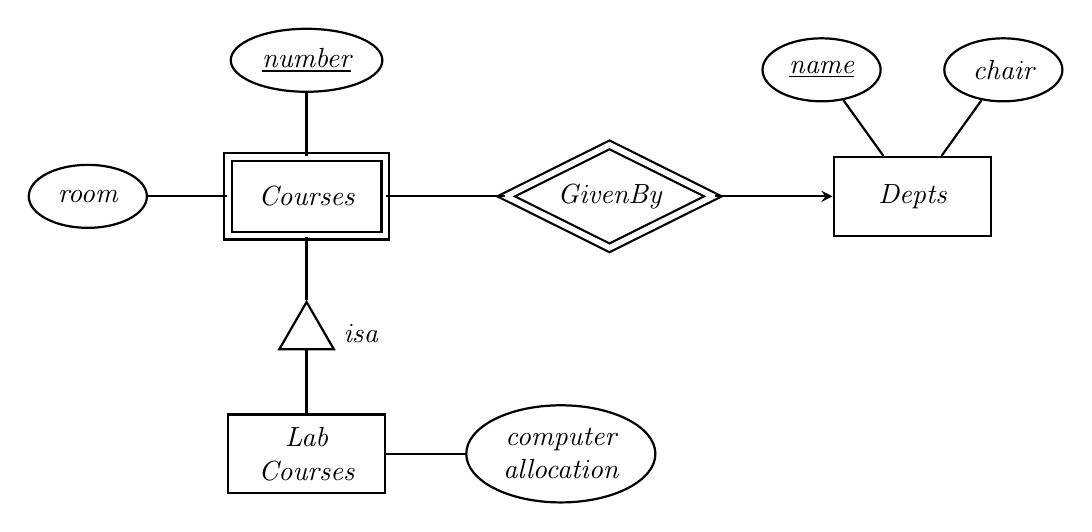
\begin{tikzpicture}[
        >=stealth, % Arrow style
        % Define node styles
        entity/.style={draw, thick, rectangle, minimum width=2cm, minimum height=1cm, align=center, font=\itshape},
        weak entity/.style={entity, double, double distance=2pt},
        relationship/.style={draw, thick, diamond, aspect=2, minimum width=2.5cm, minimum height=1.2cm, align=center, font=\itshape},
        weak relationship/.style={relationship, double, double distance=2pt},
        attribute/.style={draw, thick, ellipse, minimum width=1.5cm, minimum height=0.8cm, align=center, font=\itshape},
        isa/.style={draw, thick, regular polygon, regular polygon sides=3, minimum size=0.8cm, inner sep=0pt}
    ]
    
    % --- Entities & Relationships ---
    
    % Center Weak Entity
    \node[weak entity] (Courses) {Courses};
    
    % Identifying Relationship (Double Diamond)
    \node[weak relationship, right=1.5cm of Courses] (GivenBy) {GivenBy};
    
    % Regular Entity
    \node[entity, right=1.5cm of GivenBy] (Depts) {Depts};
    
    % ISA Hierarchy (Triangle)
    \node[isa, below=0.8cm of Courses] (isa_triangle) {};
    \node[right=0.1cm of isa_triangle, font=\itshape] {isa}; % Label next to triangle
    
    % Subclass Entity
    \node[entity, below=0.8cm of isa_triangle] (LabCourses) {Lab\\Courses};
    
    
    % --- Attributes ---
    
    % Courses Attributes
    \node[attribute, above=0.8cm of Courses] (number) {\underline{number}};
    \node[attribute, left=1cm of Courses] (room) {room};
    
    % Depts Attributes
    \node[attribute, above left=0.8cm and -0.4cm of Depts] (name) {\underline{name}};
    \node[attribute, above right=0.8cm and -0.4cm of Depts] (chair) {chair};
    
    % Lab Courses Attributes
    \node[attribute, right=1cm of LabCourses] (comp) {computer\\allocation};
    
    
    % --- Connecting Lines ---
    
    % Courses connections
    \draw[thick] (Courses) -- (number);
    \draw[thick] (Courses) -- (room);
    \draw[thick] (Courses) -- (GivenBy);
    
    % GivenBy to Depts (Many-to-One Arrow)
    \draw[thick, ->] (GivenBy) -- (Depts); 
    
    % Depts connections
    \draw[thick] (Depts) -- (name);
    \draw[thick] (Depts) -- (chair);
    
    % ISA connections
    \draw[thick] (Courses) -- (isa_triangle.north);
    \draw[thick] (isa_triangle.south) -- (LabCourses);
    
    % Lab Courses connections
    \draw[thick] (LabCourses) -- (comp);
    
    \end{tikzpicture}
\end{center}

\mk{5} \yr{CSE 215 | L-2/T-2 | 2021--22}

\begin{tcolorbox}[enhanced,breakable,ansbox,colback=cA!4,colframe=cA,boxrule=0.8pt,arc=5pt,title={\textbf{Answer}},fonttitle=\bfseries\color{white},colbacktitle=cA]

\section*{Conversion of E/R Diagram to Relational Database Schema}

The given Entity-Relationship diagram consists of a strong entity (\textbf{Depts}), an identifying relationship (\textbf{GivenBy}), a weak entity (\textbf{Courses}), and a subclass entity (\textbf{LabCourses}) structured under an \textbf{ISA} hierarchy. 

Below is the step-by-step systemic conversion of this E/R model into a set of normalized, professional relational database schemas.

---

\subsection*{1. Analysis of E/R Component Structural Constraints}
\begin{itemize}
    \item \textbf{Depts (Strong Entity):} Contains a primary key attribute \texttt{name} and a descriptive attribute \texttt{chair}.
    \item \textbf{Courses (Weak Entity):} Has a partial key (discriminator) \texttt{number} and an attribute \texttt{room}. Its existence and identity depend completely on the strong entity \textbf{Depts} via the identifying relationship \textbf{GivenBy}.
    \item \textbf{GivenBy (Identifying Relationship):} Represents a many-to-one ($\text{Many} \to 1$) structural constraint from \textbf{Courses} to \textbf{Depts}, indicated by the directed arrow towards \textbf{Depts}.
    \item \textbf{LabCourses (Subclass via ISA):} Inherits the primary identity of the superclass \textbf{Courses} and introduces its own specialized attribute \texttt{computer\_allocation}.
\end{itemize}

---

\subsection*{2. Relational Schema Mapping}

To translate these components seamlessly without introducing redundancy or illegal null states, the relational database tables are structured as follows:

\subsubsection*{Table 1: Depts (Strong Entity Relation)}
This relation represents the department entity directly.
\begin{itemize}
    \item \textbf{Primary Key (PK):} \underline{name}
\end{itemize}
$$\text{Depts}(\underline{\text{name}}, \text{chair})$$

\subsubsection*{Table 2: Courses (Weak Entity Relation)}
A weak entity does not possess a sufficient primary key on its own. Therefore, its schema must combine its partial key (\texttt{number}) with the primary key of its identifying owner department (\texttt{dept\_name}) to create a composite primary key.
\begin{itemize}
    \item \textbf{Primary Key (PK):} (\underline{number}, \underline{dept\_name})
    \item \textbf{Foreign Key (FK):} \texttt{dept\_name} referencing $\text{Depts}(\text{name})$ with an \texttt{ON DELETE CASCADE} structural rule.
\end{itemize}
$$\text{Courses}(\underline{\text{number}}, \underline{\text{dept\_name}}, \text{room})$$

\subsubsection*{Table 3: LabCourses (Subclass Relation)}
Using the standard textbook approach for ISA specialization hierarchies, a dedicated relation is created for the subclass. It imports the entire primary key configuration of its superclass (\textbf{Courses}) to establish its own primary identity and maintain referential integrity.
\begin{itemize}
    \item \textbf{Primary Key (PK):} (\underline{number}, \underline{dept\_name})
    \item \textbf{Foreign Key (FK):} (\texttt{number}, \texttt{dept\_name}) referencing $\text{Courses}(\text{number}, \text{dept\_name})$.
\end{itemize}
$$\text{LabCourses}(\underline{\text{number}}, \underline{\text{dept\_name}}, \text{computer\_allocation})$$

---

\subsection*{3. Summary Relational Schema Table}

\renewcommand{\arraystretch}{1.5}
\begin{center}
\begin{tabular}{@{}lll@{}}
\toprule
\textbf{Relation Name} & \textbf{Attributes (Primary Key Underlined)} & \textbf{Foreign Keys \& Constraints} \\ \midrule
\textbf{Depts}         & \underline{name}, chair                      & None                                  \\
\textbf{Courses}       & \underline{number}, \underline{dept\_name}, room & \texttt{dept\_name} $\to$ \textbf{Depts}(\texttt{name})  \\
\textbf{LabCourses}    & \underline{number}, \underline{dept\_name}, computer\_allocation & (\texttt{number}, \texttt{dept\_name}) $\to$ \textbf{Courses}(\texttt{number}, \texttt{dept\_name}) \\ \bottomrule
\end{tabular}
\end{center}

\vspace{0.2cm}
\begin{tcolorbox}[sharp corners, boxrule=0.5pt, colback=gray!5, colframe=gray!60, size=small]
\textbf{Design Note:} The mapping rules state that an identifying relationship table for a weak entity (\textbf{GivenBy}) is completely redundant and absorbed into the weak entity relation itself (\textbf{Courses}). This occurs because the mapping inherently pairs every entry of \textbf{Courses} with its corresponding unique department owner via the composite foreign key attribute \texttt{dept\_name}, preventing any loss of data while minimizing join overhead.
\end{tcolorbox}

\end{tcolorbox}

\item For the given E-R diagram with entities \textbf{Teacher}, \textbf{Student}, \textbf{Course}, and weak entity \textbf{Enroll}, determine which of the following statements hold:

\begin{center}
  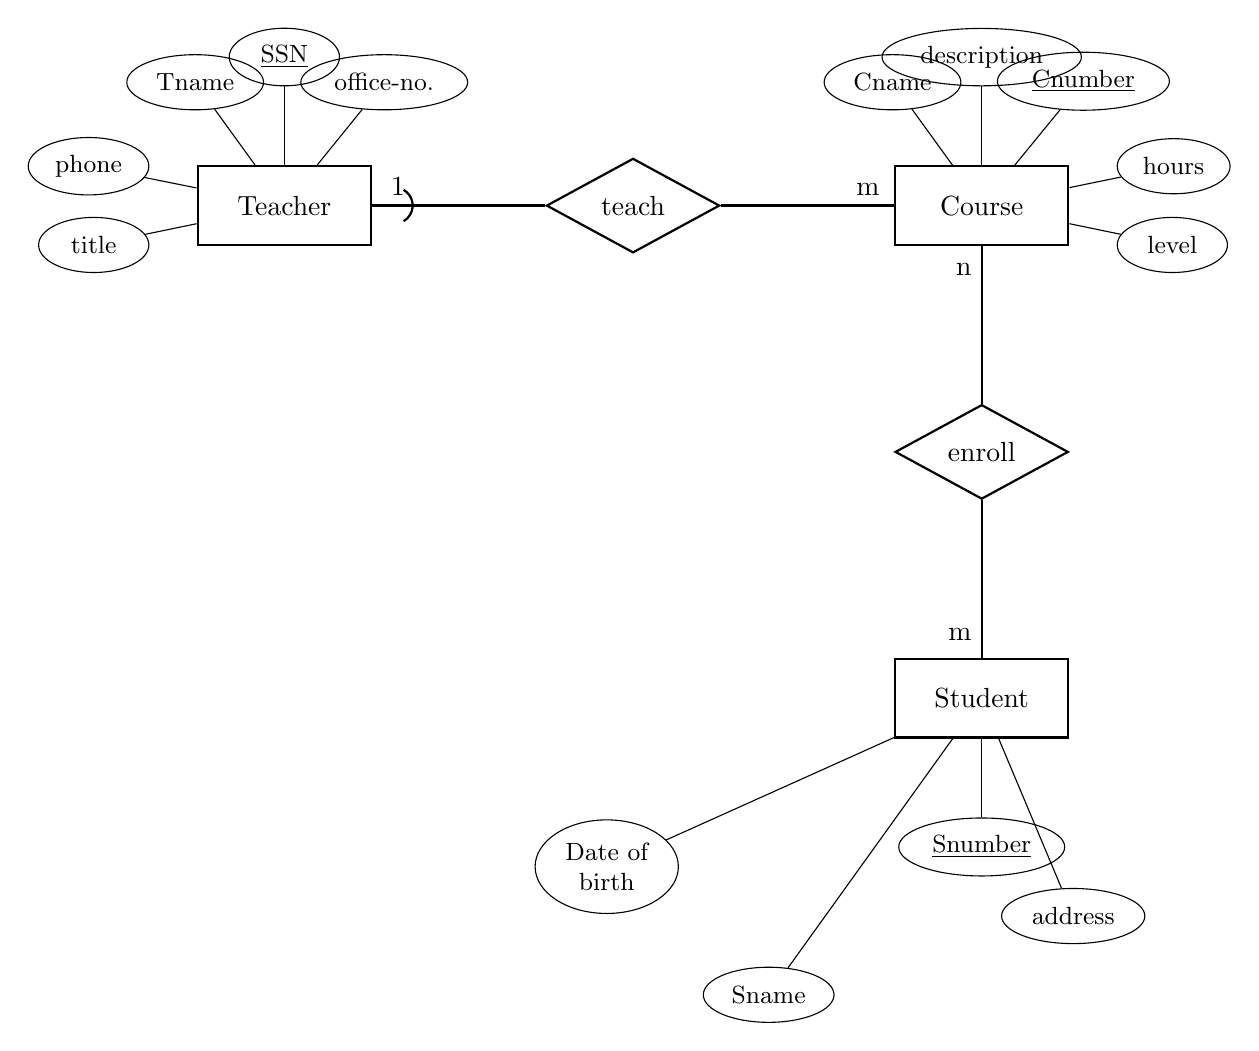
\begin{tikzpicture}[
        % Define styles for E/R diagram components
        entity/.style={draw, thick, rectangle, minimum width=2.2cm, minimum height=1cm, align=center},
        relationship/.style={draw, thick, diamond, aspect=2, minimum width=2.2cm, minimum height=1.2cm, align=center},
        attribute/.style={draw, thin, ellipse, minimum width=1.4cm, minimum height=0.7cm, align=center, font=\small}
    ]
    
    % --- ENTITIES & RELATIONSHIPS ---
    % Teacher Entity and its attributes
    \node[entity] (teacher) {Teacher};
    
    % teach Relationship
    \node[relationship, right=2.2cm of teacher] (teach) {teach};
    
    % Course Entity
    \node[entity, right=2.2cm of teach] (course) {Course};
    
    % enroll Relationship
    \node[relationship, below=2cm of course] (enroll) {enroll};
    
    % Student Entity
    \node[entity, below=2cm of enroll] (student) {Student};
    
    
    % --- ATTRIBUTES ---
    % Teacher Attributes
    \node[attribute, left=0.6cm of teacher, yshift=-0.5cm] (title) {title};
    \node[attribute, left=0.6cm of teacher, yshift=0.5cm] (phone) {phone};
    \node[attribute, above left=0.8cm and -0.6cm of teacher] (tname) {Tname};
    \node[attribute, above=1cm of teacher] (ssn) {\underline{SSN}};
    \node[attribute, above right=0.8cm and -0.6cm of teacher] (office) {office-no.};
    
    % Course Attributes
    \node[attribute, above left=0.8cm and -0.6cm of course] (cname) {Cname};
    \node[attribute, above=1cm of course] (desc) {description};
    \node[attribute, above right=0.8cm and -0.6cm of course] (cnumber) {\underline{Cnumber}};
    \node[attribute, right=0.6cm of course, yshift=0.5cm] (hours) {hours};
    \node[attribute, right=0.6cm of course, yshift=-0.5cm] (level) {level};
    
    % Student Attributes
    \node[attribute, below left=1.2cm and 3cm of student] (dob) {Date of\\birth};
    \node[attribute, below left=3cm and 1cm of student] (sname) {Sname};
    \node[attribute, below=1cm of student] (snumber) {\underline{Snumber}};
    \node[attribute, below right=2cm and -0.6cm of student] (address) {address};
    
    
    % --- CONNECTIONS & CARDINALITY ---
    % Connect Teacher to its attributes
    \draw (teacher) -- (title);
    \draw (teacher) -- (phone);
    \draw (teacher) -- (tname);
    \draw (teacher) -- (ssn);
    \draw (teacher) -- (office);
    
    % Connect Course to its attributes
    \draw (course) -- (cname);
    \draw (course) -- (desc);
    \draw (course) -- (cnumber);
    \draw (course) -- (hours);
    \draw (course) -- (level);
    
    % Connect Student to its attributes
    \draw (student) -- (dob);
    \draw (student) -- (sname);
    \draw (student) -- (snumber);
    \draw (student) -- (address);
    
    % Connect Entities via Relationships with Cardinality Labels
    % Teacher to teach (with optional arc indicator simulation)
    \draw[thick] (teacher) -- node[above, pos=0.15] {1} (teach);
    % Small arc indicator next to Teacher
    \draw[thick] ([xshift=4mm, yshift=2mm]teacher.east) arc (60:-60:2.3mm);
    
    \draw[thick] (teach) -- node[above, pos=0.85] {m} (course);
    
    % Course to Student via enroll
    \draw[thick] (course) -- node[left, pos=0.15] {n} (enroll);
    \draw[thick] (enroll) -- node[left, pos=0.85] {m} (student);
    
    \end{tikzpicture}
\end{center}

\begin{enumerate}
  \item Enroll is a strong entity set.
  \item All teachers must teach courses.
  \item All students must enroll in courses.
  \item All courses must be enrolled by students.
  \item All courses must be taught by teachers.
  \item Each course is taught by only one teacher.
  \item Each course is enrolled by only one student.
  \item Each teacher may teach many courses.
  \item Each student can enroll in many courses.
  \item Teacher is a relationship set.
\end{enumerate}
\mk{10} \yr{CSE 215 | L-2/T-2 | 2020--21}

\begin{tcolorbox}[enhanced,breakable,ansbox,colback=cA!4,colframe=cA,boxrule=0.8pt,arc=5pt,title={\textbf{Answer}},fonttitle=\bfseries\color{white},colbacktitle=cA]

\section*{Evaluation of Statements Based on the E-R Diagram}

Based on standard Entity-Relationship (E-R) modeling semantics depicted in the diagram, we analyze the structural constraints (cardinality and participation) and object types to determine the validity of each statement. 

\begin{itemize}
    \item \textbf{Rectangles} represent \textbf{Entity Sets} (Teacher, Course, Student).
    \item \textbf{Diamonds} represent \textbf{Relationship Sets} (teach, enroll).
    \item \textbf{Numbers/Letters on edges} (\textbf{1, m, n}) denote \textbf{Cardinality Ratios}.
    \item \textbf{Single lines} denote \textbf{Partial Participation} (optional), whereas double lines would denote total participation (mandatory).
\end{itemize}

Here is the evaluation of each statement:

\begin{enumerate}
    \item \textbf{Enroll is a strong entity set.} \\
    \textbf{False.} In the diagram, \textbf{enroll} is enclosed in a diamond, which dictates that it is a \textbf{relationship set}, not an entity set. Furthermore, it connects the \textbf{Course} and \textbf{Student} entity sets.
    
    \item \textbf{All teachers must teach courses.} \\
    \textbf{False.} The connection between the \textbf{Teacher} entity and the \textbf{teach} relationship is drawn with a single line. A single line indicates \textbf{partial (optional) participation}, meaning there can be teachers who do not teach any courses.
    
    \item \textbf{All students must enroll in courses.} \\
    \textbf{False.} The connection between \textbf{Student} and \textbf{enroll} is a single line, indicating partial participation.
    
    \item \textbf{All courses must be enrolled by students.} \\
    \textbf{False.} The connection between \textbf{Course} and \textbf{enroll} is a single line, indicating partial participation.
    
    \item \textbf{All courses must be taught by teachers.} \\
    \textbf{False.} The connection between \textbf{Course} and \textbf{teach} is a single line, indicating partial participation. (A course may exist in the catalog without an assigned teacher).
    
    \item \textbf{Each course is taught by only one teacher.} \\
    \textbf{True.} The cardinality ratio for the \textbf{teach} relationship is \textbf{1:m} (1 on the Teacher side, $m$ on the Course side). This means a single teacher can teach many courses, but any given course maps back to at most \textbf{one} teacher.
    
    \item \textbf{Each course is enrolled by only one student.} \\
    \textbf{False.} The cardinality ratio for the \textbf{enroll} relationship is \textbf{n:m} (many-to-many). Therefore, a single course can have multiple students enrolled in it.
    
    \item \textbf{Each teacher may teach many courses.} \\
    \textbf{True.} The \textbf{m} on the \textbf{Course} side of the \textbf{1:m} \textbf{teach} relationship indicates that a single teacher entity can be associated with multiple course entities.
    
    \item \textbf{Each student can enroll in many courses.} \\
    \textbf{True.} The \textbf{n:m} cardinality of the \textbf{enroll} relationship dictates that a student can be associated with multiple courses, just as a course can have multiple students.
    
    \item \textbf{Teacher is a relationship set.} \\
    \textbf{False.} \textbf{Teacher} is enclosed in a rectangle, which defines it as an \textbf{entity set}, not a relationship set.
\end{enumerate}

\vspace{0.5cm}

\subsection*{Summary of Valid Statements}
Only the following statements hold true for the given E-R Diagram:
\begin{itemize}
    \item \textbf{Statement 6:} Each course is taught by only one teacher.
    \item \textbf{Statement 8:} Each teacher may teach many courses.
    \item \textbf{Statement 9:} Each student can enroll in many courses.
\end{itemize}

\end{tcolorbox}

\item You are running a startup company allowing users to post blogs and comment on other users' blogs.
\begin{enumerate}
  \item Design the E/R diagram for your company's data. Store information about users, bloggers, and blogs. Every user has a user ID and a name. Every blog has a blog ID, text content, and one author (a blogger). Every blogger is a user with a rating attribute. Users may comment on blogs. Every comment has optional text content and/or an optional rating.
  \item Write a sequence of SQL queries that create the tables for this E/R diagram; \texttt{uid}, \texttt{bid}, and \texttt{rating} are integers, all other attributes are text. Include key, foreign key, and not null declarations.
\end{enumerate}
\mk{20} \yr{CSE 215 | L-2/T-2 | 2020--21}

\begin{tcolorbox}[enhanced,breakable,ansbox,colback=cA!4,colframe=cA,boxrule=0.8pt,arc=5pt,title={\textbf{Answer}},fonttitle=\bfseries\color{white},colbacktitle=cA]

\section*{Part (a): Enhanced Entity-Relationship (EER) Diagram Design}

\subsection*{1. Analysis of Entities, Attributes, and Structural Constraints}
\begin{itemize}
    \item \textbf{USER (Superclass Entity):} Contains primary key attribute \texttt{userID} and descriptive attribute \texttt{name}.
    \item \textbf{BLOGGER (Subclass Entity via ISA Hierarchy):} Represents a specialized role of a \textbf{USER}. It inherits all attributes of \textbf{USER} and contains a unique specific attribute \texttt{rating}. The specialization is \textbf{total} (every blogger must be a user) and \textbf{disjoint/single-subclass} in this context.
    \item \textbf{BLOG (Strong Entity):} Contains primary key attribute \texttt{blogID} and descriptive attribute \texttt{textContent}.
    \item \textbf{Authored\_By (Relationship):} A many-to-one ($\text{N}:1$) relationship connecting \textbf{BLOG} to \textbf{BLOGGER}. Each blog must have exactly one author (\textbf{total participation} on the \textbf{BLOG} side).
    \item \textbf{Comment (Relationship Set with Attributes):} A many-to-many ($\text{M}:\text{N}$) relationship linking \textbf{USER} and \textbf{BLOG}. It captures the scenario where users place comments on blogs. It contains descriptive attributes: \texttt{commentText} (optional) and \texttt{commentRating} (optional).
\end{itemize}

\subsection*{2. Diagram Layout Planning}
To maximize symmetry and minimize line crossings, a hierarchical vertical layout is used:
\begin{itemize}
    \item The \textbf{USER} entity is placed at the top center.
    \item An \textbf{ISA} triangle points from the subclass \textbf{BLOGGER} upward to its superclass \textbf{USER}.
    \item The \textbf{BLOG} entity is positioned on the right side.
    \item The $\text{M}:\text{N}$ relationship \textbf{Comment} sits symmetrically between \textbf{USER} and \textbf{BLOG}.
    \item The $\text{N}:1$ relationship \textbf{Authored\_By} is positioned clearly between \textbf{BLOG} and \textbf{BLOGGER}.
\end{itemize}

\begin{center}
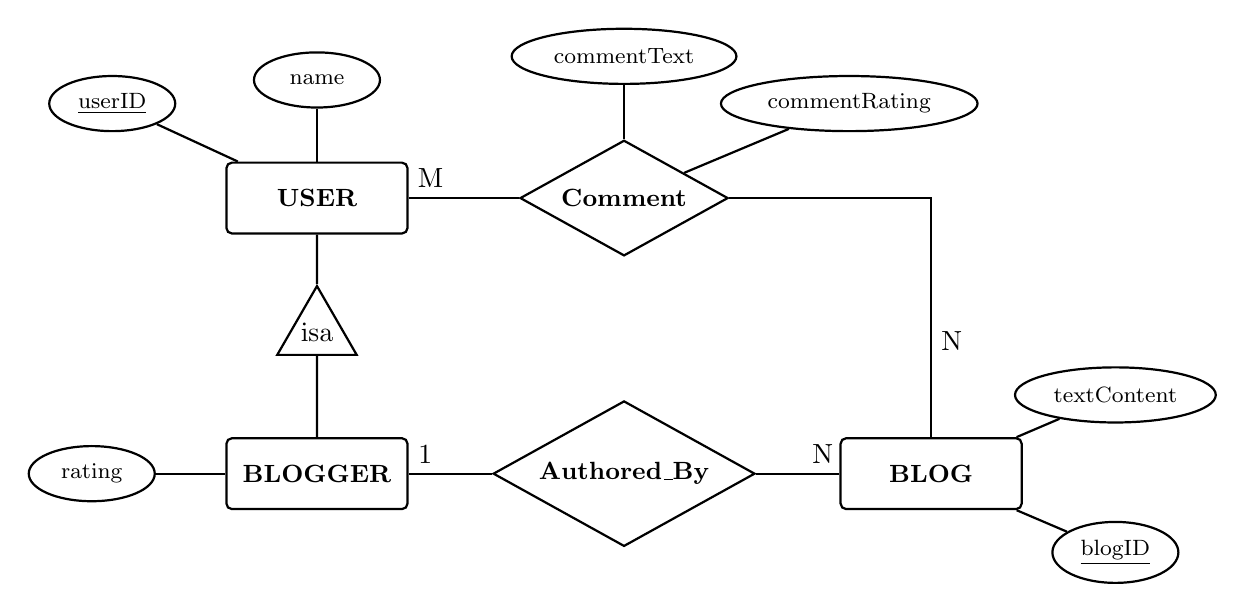
\begin{tikzpicture}[
x=1.3cm,
    entity/.style={draw, rectangle, thick, minimum width=2.3cm, minimum height=0.9cm, align=center, rounded corners=2pt, font=\small\bfseries},
    relationship/.style={draw, diamond, thick, aspect=1.8, minimum width=2.2cm, minimum height=0.9cm, align=center, font=\small\bfseries},
    attribute/.style={draw, ellipse, thick, minimum width=1.6cm, minimum height=0.7cm, align=center, font=\footnotesize},
    isa/.style={draw, regular polygon, regular polygon sides=3, thick, minimum size=0.7cm, inner sep=0pt, shape border rotate=0},
    line/.style={draw, thick}
]

    % --- Upper Level: USER Superclass ---
    \node[entity] (user) at (0, 3) {USER};
    \node[attribute] (uid) at (-2, 4.2) {\underline{userID}};
    \node[attribute] (uname) at (0, 4.5) {name};
    \draw[line] (user) -- (uid);
    \draw[line] (user) -- (uname);

    % --- ISA Hierarchy Connection ---
    \node[isa] (isa_tri) at (0, 1.3) {isa};
    \draw[line] (user.south) -- (isa_tri.north);

    % --- Lower Level Left: BLOGGER Subclass ---
    \node[entity] (blogger) at (0, -0.5) {BLOGGER};
    \node[attribute] (brating) at (-2.2, -0.5) {rating};
    \draw[line] (isa_tri.south) -- (blogger.north);
    \draw[line] (blogger) -- (brating);

    % --- Right Side: BLOG Entity ---
    \node[entity] (blog) at (6, -0.5) {BLOG};
    \node[attribute] (bid) at (7.8, -1.5) {\underline{blogID}};
    \node[attribute] (btext) at (7.8, 0.5) {textContent};
    \draw[line] (blog) -- (bid);
    \draw[line] (blog) -- (btext);

    % --- Relationship 1: Authored_By (N:1) ---
    \node[relationship] (author) at (3, -0.5) {Authored\_By};
    \draw[line] (blog) -- node[above, pos=0.2] {N} (author);
    \draw[line] (author) -- node[above, pos=0.8] {1} (blogger);

    % --- Relationship 2: Comment (M:N) ---
    \node[relationship] (comment) at (3, 3) {Comment};
    \node[attribute] (ctext) at (3, 4.8) {commentText};
    \node[attribute] (crating) at (5.2, 4.2) {commentRating};
    \draw[line] (comment) -- (ctext);
    \draw[line] (comment) -- (crating);
    
    % Connections for Comment
    \draw[line] (user) -- node[above, pos=0.2] {M} (comment);
    \draw[line] (comment) -| node[right, pos=0.8] {N} (blog.north);

\end{tikzpicture}
\end{center}

---

\section*{Part (b): Relational Schema \& Data Definition Language (DDL)}

\subsection*{1. Mapping Strategy}
\begin{itemize}
    \item \textbf{Avoidance of Nulls via Subclass Table Mapping:} To implement the \textbf{USER-BLOGGER} hierarchy cleanly without causing structural \texttt{NULL} entries for regular users who are not bloggers, a separate \texttt{Blogger} table is defined. The primary key \texttt{uid} references \texttt{Users(uid)}.
    \item \textbf{Many-to-One Linkage:} The \texttt{Blogs} table integrates its structural author dependency directly via a \texttt{NOT NULL} foreign key reference \texttt{author\_id} mapping to \texttt{Blogger(uid)}.
    \item \textbf{Many-to-Many Linkage with Attributes:} The \textbf{Comment} relationship translates into a dedicated intersection table \texttt{Comments} utilizing a composite key setup (\texttt{uid}, \texttt{bid}, \texttt{comment\_id} to support multiple comments by a single user on a single blog).
\end{itemize}

\subsection*{2. SQL Execution Script}
\begin{lstlisting}[language=SQL]
-- Create table for Superclass USER
CREATE TABLE Users (
    uid INTEGER,
    name TEXT NOT NULL,
    PRIMARY KEY (uid)
);

-- Create table for Subclass BLOGGER
CREATE TABLE Blogger (
    uid INTEGER,
    rating INTEGER NOT NULL,
    PRIMARY KEY (uid),
    FOREIGN KEY (uid) REFERENCES Users(uid) ON DELETE CASCADE
);

-- Create table for Entity BLOG
CREATE TABLE Blogs (
    bid INTEGER,
    textContent TEXT NOT NULL,
    author_id INTEGER NOT NULL,
    PRIMARY KEY (bid),
    FOREIGN KEY (author_id) REFERENCES Blogger(uid)
);

-- Create table for Relationship Set Comment (M:N Linkage)
CREATE TABLE Comments (
    comment_id INTEGER,
    uid INTEGER NOT NULL,
    bid INTEGER NOT NULL,
    commentText TEXT,
    commentRating INTEGER,
    PRIMARY KEY (comment_id),
    FOREIGN KEY (uid) REFERENCES Users(uid) ON DELETE CASCADE,
    FOREIGN KEY (bid) REFERENCES Blogs(bid) ON DELETE CASCADE
);
\end{lstlisting}

\end{tcolorbox}

\item Consider a multi-way relationship between \textbf{Actor}, \textbf{Film} and \textbf{Studio}.
\begin{enumerate}
  \item There is an arrow pointing to entity set Studios. What is its interpretation?
  \item There are no arrows pointing to entity sets Actor or Film. What are their interpretations?
\end{enumerate}
\begin{center}
  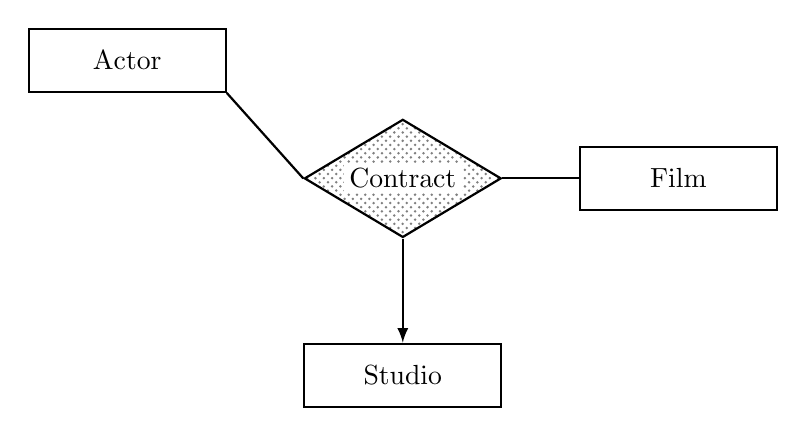
\begin{tikzpicture}[
        thick,
        % Define styles for the boxes and diamond
        entity/.style={draw, rectangle, minimum width=2.5cm, minimum height=0.8cm, align=center},
        relationship/.style={draw, diamond, aspect=1.5, minimum width=2.5cm, minimum height=1.5cm, align=center, pattern=crosshatch dots, pattern color=gray}
    ]
    
    % Draw the central relationship diamond
    \node[relationship] (contract) at (0,0) {};
    % Place the text over a white background so it is legible against the pattern
    \node at (contract) [fill=white, inner sep=2pt] {Contract};
    
    % Draw the entity nodes
    \node[entity] (actor) at (-3.5, 1.5) {Actor};
    \node[entity] (film) at (3.5, 0) {Film};
    \node[entity] (studio) at (0, -2.5) {Studio};
    
    % Draw the connecting lines
    \draw (actor.south east) -- (contract.west);
    \draw (contract.east) -- (film.west);
    \draw[-latex] (contract.south) -- (studio.north);
    
    \end{tikzpicture}
\end{center}

\mk{5} \yr{CSE 215 | L-2/T-2 | 2020--21}

\begin{tcolorbox}[enhanced,breakable,ansbox,colback=cA!4,colframe=cA,boxrule=0.8pt,arc=5pt,title={\textbf{Answer}},fonttitle=\bfseries\color{white},colbacktitle=cA]

\begin{center}
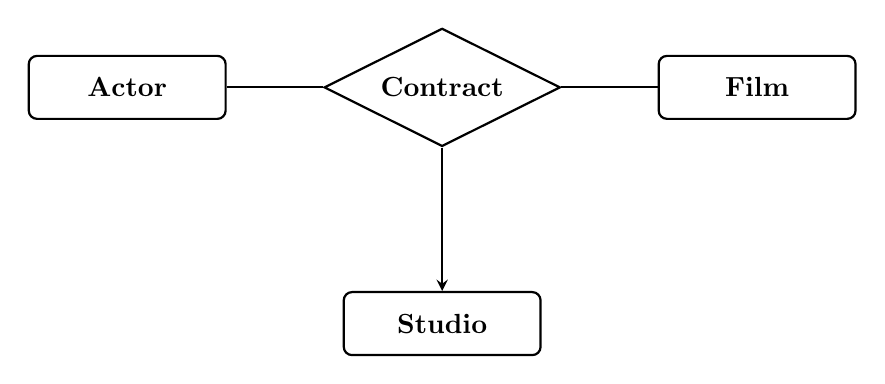
\begin{tikzpicture}[
    thick,
    entity/.style={draw, rectangle, rounded corners=3pt, minimum width=2.5cm, minimum height=0.8cm, align=center, font=\bfseries},
    relationship/.style={draw, diamond, aspect=2, minimum width=3cm, minimum height=1.5cm, align=center, font=\bfseries}
]
    % Central Relationship
    \node[relationship] (contract) at (0,0) {Contract};
    
    % Entities
    \node[entity] (actor) at (-4, 0) {Actor};
    \node[entity] (film) at (4, 0) {Film};
    \node[entity] (studio) at (0, -3) {Studio};
    
    % Connections
    \draw (actor) -- (contract);
    \draw (film) -- (contract);
    \draw[-stealth, thick] (contract) -- (studio);
\end{tikzpicture}
\end{center}

\vspace{0.5cm}

\section*{Interpretation of the Multi-way E/R Diagram}

In Entity-Relationship (E/R) modeling, a ternary (3-way) relationship connects three entity sets. The presence or absence of arrows on the edges dictates the \textbf{cardinality constraints} (or key constraints) of the relationship.

\subsection*{(a) Interpretation of the arrow pointing to Studios}
\begin{itemize}
    \item \textbf{Definition:} An arrow pointing from a multi-way relationship to an entity set indicates a \textbf{functional dependency} (a ``many-to-one'' constraint from the perspective of the other combined entities).
    \item \textbf{Interpretation:} For any given \textbf{Actor} and \textbf{Film} combination, there is \textbf{at most one} associated \textbf{Studio}. 
    \item \textbf{Explanation:} If we know the actor and the film they are starring in, that specific contract uniquely identifies exactly one studio. An actor cannot be contracted by two different studios for the exact same film.
\end{itemize}

\subsection*{(b) Interpretation of no arrows pointing to Actor or Film}
\begin{itemize}
    \item \textbf{Definition:} A standard undirected line (no arrow) in a multi-way relationship indicates a ``many'' cardinality constraint for that entity set relative to the others.
    \item \textbf{Interpretation for Actor:} For a specific \textbf{Film} and \textbf{Studio} combination, there can be \textbf{many Actors}. 
    \begin{itemize}
        \item \textit{Explanation:} A studio producing a specific film will logically sign contracts with multiple actors for that single movie.
    \end{itemize}
    \item \textbf{Interpretation for Film:} For a specific \textbf{Actor} and \textbf{Studio} combination, there can be \textbf{many Films}.
    \begin{itemize}
        \item \textit{Explanation:} A single actor can sign contracts with the same studio to appear in multiple different films over time.
    \end{itemize}
\end{itemize}

\vspace{0.2cm}
\begin{tcolorbox}[sharp corners, boxrule=0.5pt, colback=gray!5, colframe=gray!60, size=small]
\textbf{Note on Relational Translation:} If we were to convert this ternary relationship into a relational database schema, the primary key for the \texttt{Contract} table would be the composite of the primary keys of the entities without arrows: \textbf{(\underline{Actor\_ID}, \underline{Film\_ID})}. The \texttt{Studio\_ID} would simply be a non-key foreign key attribute in this table, perfectly reflecting the rule that $(\text{Actor}, \text{Film}) \rightarrow \text{Studio}$.
\end{tcolorbox}

\end{tcolorbox}

\item Consider the following information about a university database:
\begin{itemize}[leftmargin=1.5em,itemsep=1pt]
  \item Professors have an SSN, a name, an age, a rank, and a research specialty.
  \item Projects have a project number, a sponsor name, a starting date, an ending date, and a budget.
  \item Graduate students have an SSN, a name, an age, and a degree program (e.g., M.S.\ or Ph.D.).
  \item Each project is managed by one professor (principal investigator) and worked on by one or more professors (co-investigators).
  \item Each project is worked on by one or more graduate students (research assistants); a professor must supervise their work. Graduate students can work on multiple projects with a (potentially different) supervisor for each.
  \item Departments have a department number, name, and main office; a professor (chairman) runs the department.
  \item Professors work in one or more departments with an associated time percentage.
  \item Graduate students have one major department and a more senior graduate student advisor.
  \item Both professors and graduate students have multiple phone numbers and email addresses.
\end{itemize}
\begin{enumerate}
  \item Draw an ER diagram that captures the above information. Indicate all key and cardinality constraints and any assumptions you make.
  \item Convert the above ER diagram into relational schema.
\end{enumerate}
\mk{35} \yr{CSE 215 | L-2/T-2 | 2019--20}

\begin{tcolorbox}[enhanced,breakable,ansbox,colback=cA!4,colframe=cA,boxrule=0.8pt,arc=5pt,title={\textbf{Answer}},fonttitle=\bfseries\color{white},colbacktitle=cA]

\section*{Part 1: Entity-Relationship (ER) Diagram}

\textbf{Design Assumptions \& Modeling Choices:}
\begin{itemize}
    \item \textbf{Ternary Relationship:} The requirement stating \textit{"Each project is worked on by one or more graduate students; a professor must supervise their work... with a (potentially different) supervisor for each"} is modeled as a ternary relationship \textbf{Supervises\_Work} between \texttt{Professor}, \texttt{Project}, and \texttt{GradStudent}.
    \item \textbf{Multivalued Attributes:} Both \texttt{Professor} and \texttt{GradStudent} have multiple phone numbers and email addresses. These are represented as double ellipses.
    \item \textbf{Recursive Relationship:} \texttt{GradStudent} has a recursive relationship \textbf{Advises} to represent the senior advisor structure.
    \item \textbf{1:1 and M:N Roles:} \textbf{Runs} is assumed to be 1:1 (one chairman per department). \textbf{Works\_In} is an M:N relationship with a descriptive attribute \texttt{time\_percentage}.
\end{itemize}

\vspace{0.5cm}

\begin{center}

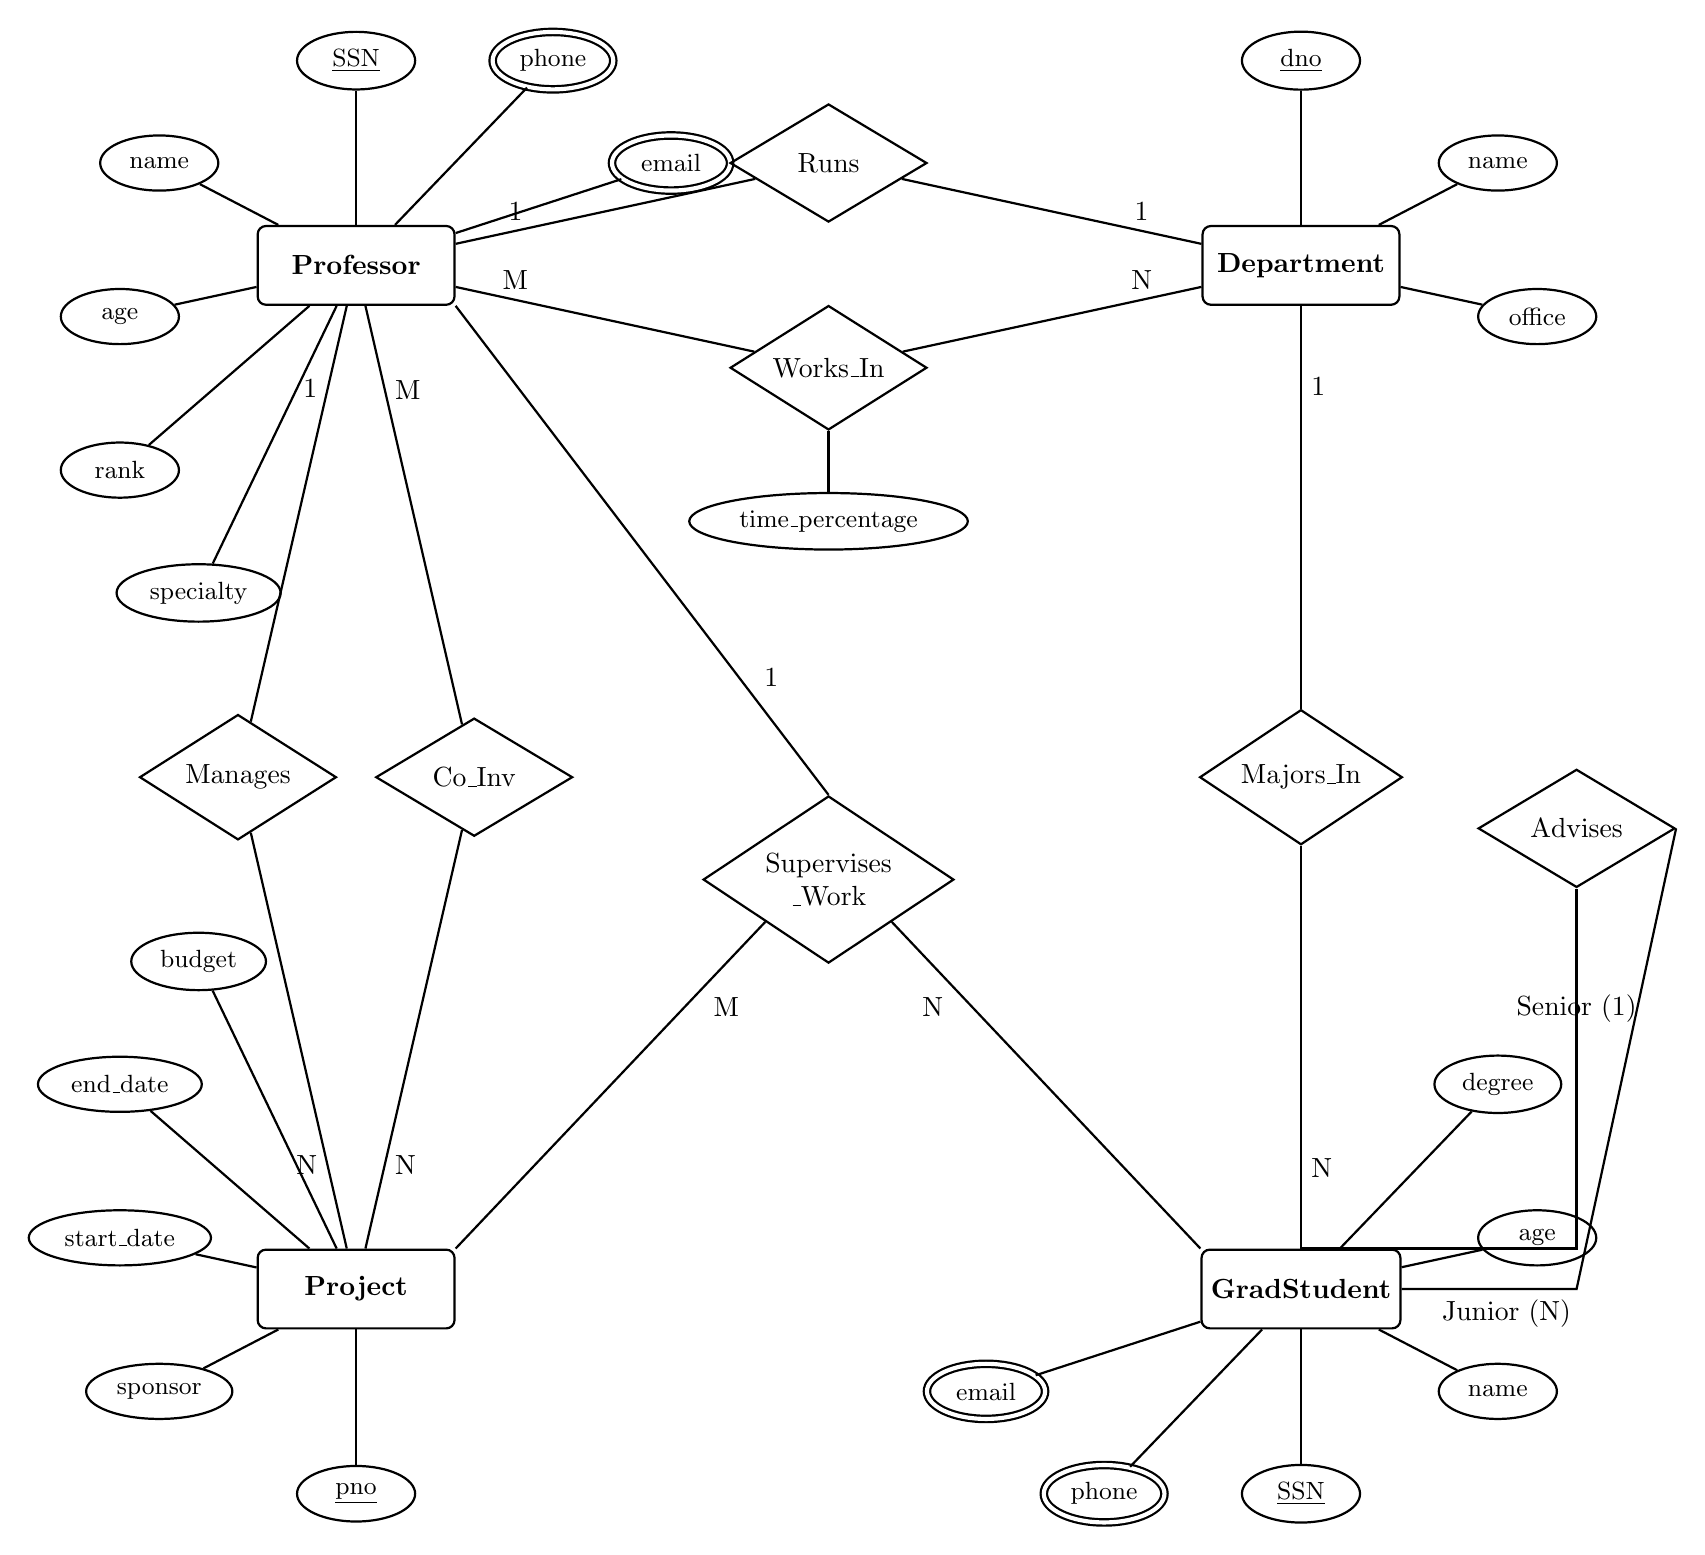
\begin{tikzpicture}[
y=1.3cm,
    entity/.style={rectangle, draw, thick, minimum width=2.5cm, minimum height=1cm, align=center, rounded corners=3pt, font=\bfseries},
    relationship/.style={diamond, draw, thick, aspect=1.5, minimum width=2.5cm, minimum height=1.5cm, align=center},
    attribute/.style={ellipse, draw, thick, align=center, minimum width=1.5cm, minimum height=0.7cm, font=\small},
    mvattribute/.style={ellipse, draw, thick, double, double distance=1.5pt, align=center, minimum width=1.5cm, minimum height=0.7cm, font=\small},
    line/.style={draw, thick}
]

    % ================= ENTITIES =================
    \node[entity] (Prof) at (-6, 5) {Professor};
    \node[entity] (Dept) at (6, 5) {Department};
    \node[entity] (Proj) at (-6, -5) {Project};
    \node[entity] (Grad) at (6, -5) {GradStudent};

    % ================= ATTRIBUTES =================
    
    % Professor Attributes
    \node[attribute] (p_ssn) at (-6, 7) {\underline{SSN}};
    \node[attribute] (p_name) at (-8.5, 6) {name};
    \node[attribute] (p_age) at (-9, 4.5) {age};
    \node[attribute] (p_rank) at (-9, 3) {rank};
    \node[attribute] (p_spec) at (-8, 1.8) {specialty};
    \node[mvattribute] (p_phone) at (-3.5, 7) {phone};
    \node[mvattribute] (p_email) at (-2, 6) {email};

    \draw[line] (Prof) -- (p_ssn);
    \draw[line] (Prof) -- (p_name);
    \draw[line] (Prof) -- (p_age);
    \draw[line] (Prof) -- (p_rank);
    \draw[line] (Prof) -- (p_spec);
    \draw[line] (Prof) -- (p_phone);
    \draw[line] (Prof) -- (p_email);

    % Department Attributes
    \node[attribute] (d_dno) at (6, 7) {\underline{dno}};
    \node[attribute] (d_name) at (8.5, 6) {name};
    \node[attribute] (d_off) at (9, 4.5) {office};

    \draw[line] (Dept) -- (d_dno);
    \draw[line] (Dept) -- (d_name);
    \draw[line] (Dept) -- (d_off);

    % Project Attributes
    \node[attribute] (pr_pno) at (-6, -7) {\underline{pno}};
    \node[attribute] (pr_spon) at (-8.5, -6) {sponsor};
    \node[attribute] (pr_start) at (-9, -4.5) {start\_date};
    \node[attribute] (pr_end) at (-9, -3) {end\_date};
    \node[attribute] (pr_budg) at (-8, -1.8) {budget};

    \draw[line] (Proj) -- (pr_pno);
    \draw[line] (Proj) -- (pr_spon);
    \draw[line] (Proj) -- (pr_start);
    \draw[line] (Proj) -- (pr_end);
    \draw[line] (Proj) -- (pr_budg);

    % GradStudent Attributes
    \node[attribute] (g_ssn) at (6, -7) {\underline{SSN}};
    \node[attribute] (g_name) at (8.5, -6) {name};
    \node[attribute] (g_age) at (9, -4.5) {age};
    \node[attribute] (g_deg) at (8.5, -3) {degree};
    \node[mvattribute] (g_phone) at (3.5, -7) {phone};
    \node[mvattribute] (g_email) at (2, -6) {email};

    \draw[line] (Grad) -- (g_ssn);
    \draw[line] (Grad) -- (g_name);
    \draw[line] (Grad) -- (g_age);
    \draw[line] (Grad) -- (g_deg);
    \draw[line] (Grad) -- (g_phone);
    \draw[line] (Grad) -- (g_email);

    % ================= RELATIONSHIPS =================

    % Prof - Dept Relationships
    \node[relationship] (Runs) at (0, 6) {Runs};
    \node[relationship] (WorksIn) at (0, 4) {Works\_In};
    \node[attribute] (time_pct) at (0, 2.5) {time\_percentage};
    \draw[line] (WorksIn) -- (time_pct);

    \draw[line] (Prof) -- node[above, pos=0.2] {1} (Runs);
    \draw[line] (Runs) -- node[above, pos=0.8] {1} (Dept);

    \draw[line] (Prof) -- node[above, pos=0.2] {M} (WorksIn);
    \draw[line] (WorksIn) -- node[above, pos=0.8] {N} (Dept);

    % Prof - Proj Relationships
    \node[relationship] (Manages) at (-7.5, 0) {Manages};
    \node[relationship] (CoInv) at (-4.5, 0) {Co\_Inv};

    \draw[line] (Prof) -- node[left, pos=0.2] {1} (Manages);
    \draw[line] (Manages) -- node[left, pos=0.8] {N} (Proj);

    \draw[line] (Prof) -- node[right, pos=0.2] {M} (CoInv);
    \draw[line] (CoInv) -- node[right, pos=0.8] {N} (Proj);

    % Grad - Dept Relationship
    \node[relationship] (MajorsIn) at (6, 0) {Majors\_In};
    \draw[line] (Grad) -- node[right, pos=0.2] {N} (MajorsIn);
    \draw[line] (MajorsIn) -- node[right, pos=0.8] {1} (Dept);

    % Grad Recursive Relationship
    \node[relationship] (Advises) at (9.5, -0.5) {Advises};
    \draw[line] (Grad.east) -- node[below, pos=0.6] {Junior (N)} (9.5, -5) -- (Advises.east);
    \draw[line] (Grad.north) -| node[above, pos=0.8] {Senior (1)} (Advises.south);

    % Ternary Relationship (Prof, Proj, Grad)
    \node[relationship] (SupWork) at (0, -1) {Supervises\\\_Work};
    \draw[line] (Prof.south east) -- node[above right, pos=0.8] {1} (SupWork.north);
    \draw[line] (Proj.north east) -- node[below right, pos=0.8] {M} (SupWork.south west);
    \draw[line] (Grad.north west) -- node[below left, pos=0.8] {N} (SupWork.south east);

\end{tikzpicture}
\end{center}



\vspace{0.5cm}

\section*{Part 2: Relational Database Schema}

The ER diagram is mapped to the following normalized relational schemas. Primary keys are \underline{underlined}, and Foreign Keys are explicitly noted.

\begin{itemize}[itemsep=4pt]
    \item \textbf{Department}( \underline{dno}, name, office, chair\_ssn )
    \begin{itemize}[label=$\circ$, topsep=0pt, itemsep=0pt]
        \item \textit{FK: \texttt{chair\_ssn} references \textbf{Professor}(ssn)}
    \end{itemize}

    \item \textbf{Professor}( \underline{ssn}, name, age, rank, specialty )

    \item \textbf{Prof\_Phone}( \underline{ssn}, \underline{phone} )
    \begin{itemize}[label=$\circ$, topsep=0pt, itemsep=0pt]
        \item \textit{FK: \texttt{ssn} references \textbf{Professor}(ssn)}
    \end{itemize}

    \item \textbf{Prof\_Email}( \underline{ssn}, \underline{email} )
    \begin{itemize}[label=$\circ$, topsep=0pt, itemsep=0pt]
        \item \textit{FK: \texttt{ssn} references \textbf{Professor}(ssn)}
    \end{itemize}

    \item \textbf{Project}( \underline{pno}, sponsor, start\_date, end\_date, budget, pi\_ssn )
    \begin{itemize}[label=$\circ$, topsep=0pt, itemsep=0pt]
        \item \textit{FK: \texttt{pi\_ssn} references \textbf{Professor}(ssn)}
    \end{itemize}

    \item \textbf{GradStudent}( \underline{ssn}, name, age, degree\_program, major\_dno, advisor\_ssn )
    \begin{itemize}[label=$\circ$, topsep=0pt, itemsep=0pt]
        \item \textit{FK: \texttt{major\_dno} references \textbf{Department}(dno)}
        \item \textit{FK: \texttt{advisor\_ssn} references \textbf{GradStudent}(ssn)}
    \end{itemize}

    \item \textbf{Grad\_Phone}( \underline{ssn}, \underline{phone} )
    \begin{itemize}[label=$\circ$, topsep=0pt, itemsep=0pt]
        \item \textit{FK: \texttt{ssn} references \textbf{GradStudent}(ssn)}
    \end{itemize}

    \item \textbf{Grad\_Email}( \underline{ssn}, \underline{email} )
    \begin{itemize}[label=$\circ$, topsep=0pt, itemsep=0pt]
        \item \textit{FK: \texttt{ssn} references \textbf{GradStudent}(ssn)}
    \end{itemize}

    \item \textbf{Works\_In}( \underline{prof\_ssn}, \underline{dno}, time\_percentage )
    \begin{itemize}[label=$\circ$, topsep=0pt, itemsep=0pt]
        \item \textit{FK: \texttt{prof\_ssn} references \textbf{Professor}(ssn)}
        \item \textit{FK: \texttt{dno} references \textbf{Department}(dno)}
    \end{itemize}

    \item \textbf{Co\_Investigates}( \underline{prof\_ssn}, \underline{pno} )
    \begin{itemize}[label=$\circ$, topsep=0pt, itemsep=0pt]
        \item \textit{FK: \texttt{prof\_ssn} references \textbf{Professor}(ssn)}
        \item \textit{FK: \texttt{pno} references \textbf{Project}(pno)}
    \end{itemize}

    \item \textbf{Supervises\_Work}( \underline{grad\_ssn}, \underline{pno}, prof\_ssn )
    \begin{itemize}[label=$\circ$, topsep=0pt, itemsep=0pt]
        \item \textit{FK: \texttt{grad\_ssn} references \textbf{GradStudent}(ssn)}
        \item \textit{FK: \texttt{pno} references \textbf{Project}(pno)}
        \item \textit{FK: \texttt{prof\_ssn} references \textbf{Professor}(ssn)}
        \item \textbf{Note:} The primary key is (\texttt{grad\_ssn}, \texttt{pno}) because a given grad student is supervised by exactly one professor for any specific project.
    \end{itemize}
\end{itemize}

\end{tcolorbox}

\item All employees in an organization are identified by employee id. All employees must have name, address, mobile and email. An employee must be one of the following: technical or non-technical. Technical employees have the trade and year of experience. Non-technical employees have the highest degree and year of experience. Each employee is managed by a manager who is also an employee. Draw the complete ERD for this scenario. Convert the ER diagram into two different possible relational schemas.
\mk{15} \yr{CSE 215 | L-2/T-2 | 2019--20}

\begin{tcolorbox}[enhanced,breakable,ansbox,colback=cA!4,colframe=cA,boxrule=0.8pt,arc=5pt,title={\textbf{Answer}},fonttitle=\bfseries\color{white},colbacktitle=cA]

\section*{Part 1: Entity-Relationship Diagram (ERD)}

\textbf{Design Considerations \& Semantic Constraints:}
\begin{itemize}
    \item \textbf{Total and Disjoint Specialization:} The prompt explicitly states an employee \textit{"must be one of the following"}. This translates to a \textbf{Total Specialization} (denoted by a double line from the superclass to the ISA triangle) and \textbf{Disjoint Specialization} (denoted by a 'd' inside the triangle).
    \item \textbf{Recursive Relationship:} The managerial structure is represented by a unary (recursive) relationship \textbf{Manages} on the \textbf{Employee} entity. An employee can manage many subordinates (N), but each employee is managed by exactly one manager (1).
\end{itemize}

\vspace{0.5cm}

\begin{center}
\begin{tikzpicture}[
    thick,x=1.2cm, 
    entity/.style={draw, rectangle, rounded corners=3pt, minimum width=2.8cm, minimum height=1.1cm, align=center, font=\bfseries},
    relationship/.style={draw, diamond, aspect=1.3, minimum width=2.5cm, minimum height=1.3cm, align=center, font=\bfseries},
    attribute/.style={draw, ellipse, minimum width=2.2cm, minimum height=0.9cm, align=center, font=\small},
    isa/.style={draw, regular polygon, regular polygon sides=3, minimum size=0.9cm, inner sep=0pt, align=center, font=\small\bfseries}
]

    % ==========================================
    % 1. SUPERCLASS (EMPLOYEE) & ATTRIBUTES
    % ==========================================
    \node[entity] (Employee) at (0, 0) {Employee};

    % Left-side attributes
    \node[attribute] (emp_id) at (-4, 1.5) {\underline{emp\_id}};
    \node[attribute] (name) at (-4, -0.2) {name};
    
    % Right-side attributes
    \node[attribute] (mobile) at (4, 1.5) {mobile};
    \node[attribute] (email) at (4, -0.2) {email};
    \node[attribute] (address) at (0, 2) {address};

    % Attribute connections
    \draw (Employee) -- (emp_id);
    \draw (Employee) -- (name);
    \draw (Employee) -- (mobile);
    \draw (Employee) -- (email);
    \draw (Employee) -- (address);

    % ==========================================
    % 2. RECURSIVE RELATIONSHIP (MANAGES)
    % ==========================================
    % Positioned safely on the far left to eliminate crowded edge overlaps
    \node[relationship] (Manages) at (-5.5, -2.5) {Manages};
    
    % Manager Link (1)
    \draw (Employee.west) -- ++(-1.5,0) |- node[left, pos=0.25, font=\small] {1} 
          node[above right, pos=0.85, font=\scriptsize\itshape] {manager} (Manages.north);
          
    % Subordinate Link (N)
    \draw (Employee.195) -- ++(-1.1,0) |- node[left, pos=0.25, font=\small] {N} 
          node[below right, pos=0.85, font=\scriptsize\itshape] {subordinate} (Manages.east);

    % ==========================================
    % 3. SPECIALIZATION (ISA)
    % ==========================================
    \node[isa] (isa) at (0, -2.5) {d};
    
    % Total Specialization -> Double Line
    \draw[double, double distance=2.5pt] (Employee.south) -- (isa.north);

    % ==========================================
    % 4. SUBCLASSES & THEIR ATTRIBUTES
    % ==========================================
    \node[entity] (Tech) at (-4, -4.5) {Technical};
    \node[entity] (NonTech) at (4, -4.5) {Non-Technical};

    % Orthogonal structural connections to the ISA triangle
    \draw (isa.south) -- (0, -3.5) -| (Tech.north);
    \draw (isa.south) -- (0, -3.5) -| (NonTech.north);

    % Technical Attributes (Balanced Below)
    \node[attribute] (trade) at (-6, -6.2) {trade};
    \node[attribute] (texp) at (-2, -6.2) {year\_of\_exp};
    \draw (Tech) -- (trade);
    \draw (Tech) -- (texp);

    % Non-Technical Attributes (Balanced Below)
    \node[attribute] (deg) at (2, -6.2) {highest\_degree};
    \node[attribute] (nexp) at (6, -6.2) {year\_of\_exp};
    \draw (NonTech) -- (deg);
    \draw (NonTech) -- (nexp);

\end{tikzpicture}
\end{center}

\vspace{0.5cm}

---

\section*{Part 2: Relational Schema Conversion}

An ER Diagram with a Superclass/Subclass hierarchy can be mapped into a relational schema in several standard ways. Because this is a \textbf{Total and Disjoint} specialization, two highly effective and structurally distinct schemas can be produced. 

\subsection*{Option 1: Superclass/Subclass Multiple Relations (ER-to-Relational Standard)}
In this approach, the superclass and all subclasses have their own separate tables. The subclass tables inherit the primary key from the superclass, which serves as both their primary key and a foreign key.

\begin{itemize}[itemsep=5pt]
    \item \textbf{Employee} (\underline{emp\_id}, name, address, mobile, email, manager\_id)
        \begin{itemize}[label=$\circ$, topsep=0pt, itemsep=0pt]
            \item \textit{Foreign Key:} \texttt{manager\_id} references \textbf{Employee}(\texttt{emp\_id})
        \end{itemize}
    \item \textbf{Technical} (\underline{emp\_id}, trade, year\_of\_exp)
        \begin{itemize}[label=$\circ$, topsep=0pt, itemsep=0pt]
            \item \textit{Foreign Key:} \texttt{emp\_id} references \textbf{Employee}(\texttt{emp\_id})
        \end{itemize}
    \item \textbf{NonTechnical} (\underline{emp\_id}, highest\_degree, year\_of\_exp)
        \begin{itemize}[label=$\circ$, topsep=0pt, itemsep=0pt]
            \item \textit{Foreign Key:} \texttt{emp\_id} references \textbf{Employee}(\texttt{emp\_id})
        \end{itemize}
\end{itemize}
\textbf{Advantage:} Highly normalized. Eliminates `NULL` values entirely for the subclass-specific attributes.

\vspace{0.3cm}

\subsection*{Option 2: Single Universal Relation (Flattened Structure)}
Because the specialization is disjoint and total, and there are relatively few subclass-specific attributes, we can collapse the hierarchy into a single table. A discriminator attribute (\texttt{emp\_type}) is introduced, and shared attributes (like \texttt{year\_of\_exp}) are merged.

\begin{itemize}[itemsep=5pt]
    \item \textbf{Employee\_Universal} (\underline{emp\_id}, emp\_type, name, address, mobile, email, manager\_id, trade, highest\_degree, year\_of\_exp)
        \begin{itemize}[label=$\circ$, topsep=0pt, itemsep=0pt]
            \item \textit{Foreign Key:} \texttt{manager\_id} references \textbf{Employee\_Universal}(\texttt{emp\_id})
            \item \textit{Note:} \texttt{emp\_type} will store values like \texttt{'Technical'} or \texttt{'Non-Technical'}. If \texttt{'Technical'}, \texttt{highest\_degree} will be \texttt{NULL}. If \texttt{'Non-Technical'}, \texttt{trade} will be \texttt{NULL}.
        \end{itemize}
\end{itemize}
\textbf{Advantage:} Improves read performance since no expensive `JOIN` operations are required to assemble an employee's full profile.

\end{tcolorbox}

\item What do you mean by materialized view? Explain with examples the problems associated with materialized view. What restrictions do most database implementations have to allow updates on materialized views?
\mk{10} \yr{CSE 215 | L-2/T-2 | 2019--20}

\begin{tcolorbox}[enhanced,breakable,ansbox,colback=cA!4,colframe=cA,boxrule=0.8pt,arc=5pt,title={\textbf{Answer}},fonttitle=\bfseries\color{white},colbacktitle=cA]

\section*{1. Materialized View: Definition and Explanation}

\textbf{Definition:} A \textbf{materialized view} is a database object that contains the precomputed results of a query. Unlike a standard (virtual) view, which dynamically computes the result set every time it is queried by executing the underlying SQL, a materialized view permanently stores (materializes) the data on physical storage (disk).

\textbf{Working Principle:} When a materialized view is created, the database evaluates the defining query and saves the output into a physical table structure. Subsequent queries against the materialized view read directly from this physical structure, drastically reducing execution time for complex joins, aggregations, and large data scans. They are widely used in \textbf{Data Warehousing} and \textbf{Business Intelligence (BI)} systems.

\begin{center}
\renewcommand{\arraystretch}{1.3}
\begin{tabular}{@{} p{4cm} p{5.5cm} p{5.5cm} @{}}
\toprule
\textbf{Feature} & \textbf{Standard (Virtual) View} & \textbf{Materialized View} \\
\midrule
\textbf{Storage} & Stores only the SQL query definition. & Stores both the query definition and the actual data. \\
\textbf{Performance} & Slower for complex queries (recalculated every time). & Extremely fast (data is pre-computed and fetched from disk). \\
\textbf{Data Freshness} & Always up-to-date with base tables. & Can be stale; requires periodic or triggered refreshing. \\
\bottomrule
\end{tabular}
\end{center}

\vspace{0.5cm}

\section*{2. Problems Associated with Materialized Views}

While materialized views provide significant performance benefits for read-heavy workloads, they introduce several major challenges, primarily concerning \textbf{View Maintenance} (keeping the materialized data synchronized with the base tables).

\subsection*{A. The View Maintenance Problem (Data Staleness)}
When the base tables are modified (INSERT, UPDATE, DELETE), the materialized view becomes out of sync (stale). The database must update the materialized view, which can be computationally expensive.

\textbf{Example:}
Consider an e-commerce database with a materialized view that calculates total daily sales.
\begin{lstlisting}[language=SQL]
CREATE MATERIALIZED VIEW Daily_Sales_MV AS
SELECT store_id, transaction_date, SUM(amount) as total_sales
FROM Sales
GROUP BY store_id, transaction_date;
\end{lstlisting}

\begin{itemize}
    \item \textbf{Problem Scenario:} If a customer makes a new purchase, a new row is inserted into the \texttt{Sales} table. The \texttt{Daily\_Sales\_MV} is now outdated. 
    \item If the system is configured for \textbf{Immediate Refresh} (synchronous update), the insertion into the \texttt{Sales} table will be delayed because the database must simultaneously recalculate and update the materialized view. This degrades Online Transaction Processing (OLTP) performance.
    \item If configured for \textbf{Deferred Refresh} (asynchronous update, e.g., nightly), business analysts querying the view during the day will see inaccurate, stale data.
\end{itemize}

\subsection*{B. High Storage Overhead}
Because materialized views store the actual result sets, they consume significant physical disk space. A poorly designed materialized view that joins multiple massive tables without strong filtering can duplicate terabytes of data.

\subsection*{C. Write Amplification}
A single update to a base table might trigger cascading updates across multiple materialized views that depend on it, consuming excessive CPU, memory, and I/O bandwidth.

\vspace{0.5cm}

\section*{3. Restrictions on Updating Materialized Views}

To mitigate the massive cost of completely recomputing a materialized view every time a base table changes, modern DBMS implementations (like Oracle, PostgreSQL, and SQL Server) use \textbf{Incremental Maintenance} (often called \textbf{Fast Refresh}). Instead of recalculating the whole query, the DBMS only calculates the delta (the changes). 

However, to allow Fast Refresh (or to allow users to issue direct \texttt{UPDATE}/\texttt{INSERT} statements on the materialized view in updatable MV scenarios), the database enforces strict structural restrictions on the defining query:

\begin{enumerate}
    \item \textbf{Primary Key / ROWID Requirement:} The defining query must include the primary keys or internal row identifiers (\texttt{ROWID}) of all underlying base tables. This allows the database to map a changed row in the base table directly to the corresponding row in the materialized view.
    \item \textbf{Aggregate Function Limitations:} 
    \begin{itemize}
        \item If the view uses \texttt{GROUP BY}, it must usually include the \texttt{COUNT(*)} or \texttt{COUNT(column)} aggregate function. This is necessary so the database knows when to delete a row from the materialized view (i.e., when the count drops to zero after a base table deletion).
        \item Complex aggregates like \texttt{MIN}, \texttt{MAX}, or statistical functions often prevent incremental updates because removing the current "maximum" value requires scanning the entire base table to find the new maximum.
    \end{itemize}
    \item \textbf{No Non-Deterministic Functions:} The query cannot contain volatile or time-dependent functions such as \texttt{SYSDATE}, \texttt{RAND()}, or \texttt{CURRENT\_TIMESTAMP}.
    \item \textbf{Join Restrictions:} While simple equi-joins are typically supported, complex outer joins, self-joins, or joins combined heavily with aggregations often disqualify a materialized view from fast refresh.
    \item \textbf{Set Operator Restrictions:} Queries utilizing \texttt{UNION}, \texttt{INTERSECT}, or \texttt{EXCEPT} (MINUS) usually cannot be incrementally maintained.
    \item \textbf{Subquery Limitations:} Correlated subqueries or subqueries in the \texttt{SELECT} clause generally prevent fast updates.
\end{enumerate}

\textbf{Note on Direct Updates:} If referring to \textit{Updatable Materialized Views} (where a user explicitly executes \texttt{UPDATE MV\_Name SET ...}), most DBMSs forbid this entirely. Those that do support it (e.g., Oracle Advanced Replication) require strict primary key linkages and bidirectional replication logs to push the changes back to the base tables without conflict.

\end{tcolorbox}

\item Reduce the given ERD to the minimum relational schemas (mention schema names and their attributes).

\begin{center}
  \begin{tikzpicture}[
        >=Stealth, % Sets arrow style
        entity/.style={draw, rectangle, minimum width=1.5cm, minimum height=0.8cm},
        relationship/.style={draw, diamond, aspect=2, minimum width=1.5cm, minimum height=0.8cm},
        attribute/.style={draw, ellipse, minimum width=0.8cm, minimum height=0.5cm, font=\small},
        % R5 is uniquely drawn as a parallelogram in the image
        parallelogram/.style={draw, trapezium, trapezium left angle=70, trapezium right angle=110, minimum width=1.5cm, inner xsep=0pt}
    ]

    % --- Entities ---
    \node[entity] (A) at (0, 0) {A};
    \node[entity] (B) at (6, 0) {B};
    \node[entity] (C) at (0, -4) {C};
    \node[entity] (D) at (6, -4) {D};

    % --- Relationships ---
    \node[relationship] (R1) at (3, 0) {R1};
    \node[relationship] (R2) at (0, -2) {R2};
    \node[relationship] (R3) at (3, -4) {R3};
    \node[relationship] (R4) at (6, -2) {R4};
    \node[parallelogram] (R5) at (3, -2) {R5}; 

    % --- Attributes for Entity A ---
    \node[attribute] (a1) at (-0.8, 1.2) {\underline{a1}};
    \node[attribute] (a2) at (0.8, 1.2) {a2};
    \draw (A) -- (a1);
    \draw (A) -- (a2);

    % --- Attributes for Entity B ---
    \node[attribute] (b1) at (5.2, 1.2) {\underline{b1}};
    \node[attribute] (b2) at (6.8, 1.2) {b2};
    \draw (B) -- (b1);
    \draw (B) -- (b2);

    % --- Attributes for Entity C ---
    \node[attribute] (c1) at (-0.8, -5.2) {\underline{c1}};
    \node[attribute] (c2) at (0.8, -5.2) {c2};
    \draw (C) -- (c1);
    \draw (C) -- (c2);

    % --- Attributes for Entity D ---
    \node[attribute] (d1) at (5.2, -5.2) {\underline{d1}};
    \node[attribute] (d2) at (6.8, -5.2) {d2};
    \draw (D) -- (d1);
    \draw (D) -- (d2);

    % --- Edges between Entities and Relationships ---
    
    % R1: A and B
    \draw (A) -- (R1);
    \draw[<-] (R1) -- (B); % Arrow points to R1 from B

    % R2: A and C
    \draw (A) -- (R2);
    \draw (C) -- (R2);

    % R3: C and D
    \draw[<-] (R3) -- (C); % Arrow points to R3 from C
    \draw (D) -- (R3);

    % R4: B and D
    \draw[<-] (R4) -- (B); % Arrow points to R4 from B
    \draw (D) -- (R4);

    % R5: B and C
    \draw[<-] (R5) -- (B); % Arrow points to R5 from B
    \draw (C) -- (R5);

    \end{tikzpicture}
\end{center}
\mk{10} \yr{CSE 215 | L-2/T-2 | 2019--20}

\begin{tcolorbox}[enhanced,breakable,ansbox,colback=cA!4,colframe=cA,boxrule=0.8pt,arc=5pt,title={\textbf{Answer}},fonttitle=\bfseries\color{white},colbacktitle=cA]

\section*{1. Cardinality Analysis}
To reduce the given Entity-Relationship Diagram (ERD) to its minimum relational schemas, we first establish the relationship cardinalities based on standard ER conventions. In standard notations (like Korth), a directed edge (arrow) pointing to/from an entity signifies the \textbf{``1'' (One)} side of a relationship (often representing a key constraint), whereas an undirected edge (line) signifies the \textbf{``N'' (Many)} side.

Based on the structure provided in the diagram:
\begin{itemize}
    \item \textbf{R1 (between A and B):} The directed arrow on B's side indicates a \textbf{N:1} relationship from A to B (A is Many, B is 1).
    \item \textbf{R2 (between A and C):} Undirected on both sides, indicating a \textbf{M:N} (Many-to-Many) relationship.
    \item \textbf{R3 (between C and D):} The directed arrow on C's side indicates a \textbf{N:1} relationship from D to C (D is Many, C is 1).
    \item \textbf{R4 (between B and D):} The directed arrow on B's side indicates a \textbf{N:1} relationship from D to B (D is Many, B is 1).
    \item \textbf{R5 (between B and C):} The directed arrow on B's side indicates a \textbf{N:1} relationship from C to B (C is Many, B is 1). \textit{Note: Though R5 is drawn as a parallelogram in the visual, it functions as a standard mapping in this reduction.}
\end{itemize}

\section*{2. Relational Schema Reduction}
We apply the standard algorithm for ERD-to-Relational mapping:
\begin{enumerate}
    \item \textbf{Strong Entities:} Each entity receives its own table.
    \item \textbf{1:N Relationships:} The primary key of the ``1'' side is embedded as a \textbf{Foreign Key (FK)} in the table of the ``N'' side.
    \item \textbf{M:N Relationships:} A separate table is created containing the primary keys of both participating entities.
\end{enumerate}

This yields a minimum of \textbf{5 relational schemas}. Primary keys are \underline{underlined}, and foreign keys are \textit{italicized}.

\begin{itemize}[itemsep=1ex, leftmargin=2em]
    \item \textbf{B} (\underline{b1}, b2)
    \item \textbf{A} (\underline{a1}, a2, \textit{b1}) \hfill \textit{-- b1 references B(b1)}
    \item \textbf{C} (\underline{c1}, c2, \textit{b1}) \hfill \textit{-- b1 references B(b1)}
    \item \textbf{D} (\underline{d1}, d2, \textit{c1}, \textit{b1}) \hfill \textit{-- c1 references C(c1), b1 references B(b1)}
    \item \textbf{R2} (\underline{a1, c1}) \hfill \textit{-- a1 references A(a1), c1 references C(c1)}
\end{itemize}

\vspace{0.5cm}

\section*{3. Relational Schema Diagram}
\begin{center}
\begin{tikzpicture}[
    >=Stealth,x=1.4cm,
    table/.style={
        draw, thick, rectangle, rounded corners=3pt,
        align=center, minimum height=0.8cm, font=\small\ttfamily,
        fill=white
    },
    arrow/.style={->, thick, rounded corners=4pt, color=black!80}
]

% Nodes
\node[table] (B)  at (0, 4)  {\textbf{B} ( \underline{b1}, b2 )};
\node[table] (A)  at (-4, 2) {\textbf{A} ( \underline{a1}, a2, \textit{b1} )};
\node[table] (C)  at (0, 2)  {\textbf{C} ( \underline{c1}, c2, \textit{b1} )};
\node[table] (D)  at (0, 0)  {\textbf{D} ( \underline{d1}, d2, \textit{c1}, \textit{b1} )};
\node[table] (R2) at (-4, 0) {\textbf{R2} ( \underline{a1}, \underline{c1} )};

% Arrows for Foreign Keys
% A(b1) -> B(b1)
\draw[arrow] (A.north) |- (B.west);

% C(b1) -> B(b1)
\draw[arrow] (C.north) -- (B.south);

% D(c1) -> C(c1)
\draw[arrow] (D.north) -- (C.south);

% D(b1) -> B(b1) (routes around the right side to prevent overlap)
\draw[arrow] (D.east) -- ++(1.5,0) |- (B.east);

% R2(a1) -> A(a1)
\draw[arrow] (R2.north) -- (A.south);

% R2(c1) -> C(c1) (routes neatly between the columns)
\draw[arrow] (R2.east) -- ++(1,0) |- (C.west);

\end{tikzpicture}
\end{center}

\end{tcolorbox}

\item How can redundancy and incompleteness lead to a bad database design? Explain with appropriate examples.
\mk{10} \yr{CSE 215 | L-2/T-2 | 2018--19}

\begin{tcolorbox}[enhanced,breakable,ansbox,colback=cA!4,colframe=cA,boxrule=0.8pt,arc=5pt,title={\textbf{Answer}},fonttitle=\bfseries\color{white},colbacktitle=cA]

\section*{1. Introduction to Bad Database Design}
A poor database design typically suffers from two major structural deficiencies: \textbf{redundancy} (storing the same data multiple times unnecessarily) and \textbf{incompleteness} (failing to capture all required data or data relationships). In a relational database management system (RDBMS), these design flaws compromise data integrity, waste storage resources, and lead to programmatic anomalies during data manipulation.

\vspace{0.5cm}

\section*{2. Redundancy in Database Design}

\subsection*{A. Definition and Explanation}
\textbf{Data redundancy} occurs when the same piece of data is duplicated across multiple rows or tables due to an unnormalized schema. This usually happens when an entity's operational details are blended with another independent entity's attributes in a single relation.

\subsection*{B. Problems Caused by Redundancy: Data Anomalies}
Redundancy directly causes three critical data anomalies during routine database updates:
\begin{enumerate}
    \item \textbf{Insertion Anomaly:} The inability to insert critical facts about one entity without possessing completely unrelated data belonging to another entity.
    \item \textbf{Deletion Anomaly:} The unintended loss of critical independent data because a related record containing that data is deleted.
    \item \textbf{Update (Modification) Anomaly:} The requirement to modify multiple duplicate data rows when a single fact changes. Failure to update every row results in data inconsistency.
\end{enumerate}

\subsection*{C. Concrete Example of Redundancy}
Consider an unnormalized relation \texttt{Emp\_Dept} that stores both employee and department information in a single table:

\begin{center}
\small
\begin{tabular}{ccccc}
\toprule
\textbf{Emp\_ID (PK)} & \textbf{Emp\_Name} & \textbf{Role} & \textbf{Dept\_ID} & \textbf{Dept\_Name} \\
\midrule
E101 & Alice & Developer & D01 & Engineering \\
E102 & Bob   & Analyst   & D02 & Marketing \\
E103 & Charlie & Developer & D01 & Engineering \\
\bottomrule
\end{tabular}
\end{center}

\textbf{Analysis of Anomalies:}
\begin{itemize}
    \item \textbf{Update Anomaly:} If the \texttt{Dept\_Name} for \texttt{D01} changes from ``Engineering'' to ``Research \& Development'', the system must find and update both records for Alice (E101) and Charlie (E103). If one row fails to update, the database falls into an inconsistent state.
    \item \textbf{Insertion Anomaly:} Suppose the organization establishes a new department named ``Finance'' (\texttt{D03}), but has not hired any employees for it yet. Because \texttt{Emp\_ID} is the primary key and cannot accept a \texttt{NULL} value, the data for the new department cannot be recorded.
    \item \textbf{Deletion Anomaly:} If Bob (\texttt{E102}) resigns from the company and his record is deleted from the database, all knowledge that department \texttt{D02} is called ``Marketing'' is irreversibly wiped out.
\end{itemize}

\subsection*{D. Resolution via Normalization}
To correct this, the database designer decomposes the table into two separate, normalized relations connected via a foreign key relationship:

\begin{center}
\small
\textbf{Department Table}\\
\begin{tabular}{cc}
\toprule
\textbf{\underline{Dept\_ID}} & \textbf{Dept\_Name} \\
\midrule
D01 & Engineering \\
D02 & Marketing \\
\bottomrule
\end{tabular}
\end{center}

\begin{center}
\small
\textbf{Employee Table}\\
\begin{tabular}{cccc}
\toprule
\textbf{\underline{Emp\_ID}} & \textbf{Emp\_Name} & \textbf{Role} & \textbf{\textit{Dept\_ID}} \\
\midrule
E101 & Alice   & Developer & D01 \\
E102 & Bob     & Analyst   & D02 \\
E103 & Charlie & Developer & D01 \\
\bottomrule
\end{tabular}
\end{center}

\vspace{0.5cm}

\section*{3. Incompleteness in Database Design}

\subsection*{A. Definition and Explanation}
\textbf{Incompleteness} refers to a database design that fails to fully capture all business rules, requirements, historical constraints, or entity attributes. It manifests as a lack of required fields, absence of necessary relationships, or structural inability to hold multivalued or temporal states.

\subsection*{B. Problems Caused by Incompleteness}
\begin{itemize}
    \item \textbf{Loss of Information:} Inability to capture vital business transaction metrics.
    \item \textbf{Misuse of NULL Values:} Forcing attributes to hold \texttt{NULL} values when a separate structure is actually needed, degrading query optimization and clarity.
    \item \textbf{Inability to Enforce Integrity Constraints:} Critical validation checks cannot be established if key supporting attributes are absent.
\end{itemize}

\subsection*{C. Concrete Example of Incompleteness}
Consider a hospital database that tracks patients and their prescribed medications. An incomplete design places the prescribed drug directly in the \texttt{Patient} table:

\begin{center}
\small
\textbf{Patient (Incomplete Schema)}\\
\begin{tabular}{cccc}
\toprule
\textbf{\underline{Patient\_ID}} & \textbf{Patient\_Name} & \textbf{Diagnosis} & \textbf{Prescribed\_Medication} \\
\midrule
P501 & John Doe & Hypertension & Lisinopril \\
P502 & Jane Smith & Diabetes & Metformin \\
\bottomrule
\end{tabular}
\end{center}

\textbf{Analysis of Flaws:}
\begin{itemize}
    \item \textbf{Multivalued Attribute Issue:} If John Doe is diagnosed with multiple conditions and requires three different medications simultaneously, this single atomic field design breaks. Attempting to store comma-separated strings (e.g., ``Lisinopril, Amlodipine'') violates First Normal Form ($1\text{NF}$), complicating string parsing and index usage.
    \item \textbf{Loss of History:} This design lacks data fields for prescription date, structural dosage instructions (e.g., ``twice a day''), and prescribing doctor. Overwriting \texttt{Prescribed\_Medication} when a drug is changed obliterates vital historical patient medical records.
\end{itemize}

\subsection*{D. Resolution via Proper Structural Modeling}
A robust design isolates multi-valued interactions into a distinct transaction table:

\begin{center}
\small
\begin{tikzpicture}[
    >=Stealth,
    node distance=1.2cm and 2.2cm,
    entity/.style={draw, rectangle, rounded corners=2pt, minimum width=2.2cm, minimum height=0.8cm, thick, align=center},
    relationship/.style={draw, diamond, aspect=2, minimum width=2.2cm, minimum height=0.8cm, thick, align=center},
    attribute/.style={draw, ellipse, minimum width=1.6cm, minimum height=0.6cm, font=\small, align=center}
]

    % Grid Alignment Planning
    % Central nodes
    \node[entity] (patient) {PATIENT};
    \node[relationship] (presc) [right=of patient] {PRESCRIBES};
    \node[entity] (med) [right=of presc] {MEDICATION};
    
    % Attributes for PRESCRIBES relationship to model structural completeness
    \node[attribute] (date) [above=of presc] {Presc\_Date};
    \node[attribute] (dosage) [below=of presc] {Dosage};

    % Connections
    \draw[thick] (patient) -- node[above, font=\small, near start] {1} (presc);
    \draw[thick] (presc) -- node[above, font=\small, near end] {N} (med);
    \draw[thick] (presc) -- (date);
    \draw[thick] (presc) -- (dosage);

\end{tikzpicture}
\end{center}

\vspace{0.3cm}

\section*{4. Summary Comparison}

\begin{center}
\small
\renewcommand{\arraystretch}{1.3}
\begin{tabular}{lll}
\toprule
\textbf{Design Flaw} & \textbf{Primary Root Cause} & \textbf{Typical Engineering Solution} \\
\midrule
\textbf{Redundancy} & Bad decomposition / Combining independent facts & Normalization ($2\text{NF}$, $3\text{NF}$, $\text{BCNF}$) \\
\textbf{Incompleteness} & Poor requirement gathering / Violating cardinality & Comprehensive ER modeling \& schema review \\
\bottomrule
\end{tabular}
\end{center}

\end{tcolorbox}

\item Production tracking is important in many manufacturing environments (e.g., the pharmaceuticals
industry, children's toys, etc.). The ER diagram of Figure captures important
information of production tracking. Specifically, the ER diagram captures the relationships
among production lots (or batches), individual production units, and raw materials.

\begin{center}
  \begin{tikzpicture}[
        >=Stealth,
        font=\sffamily\small,
        % Styles for nodes
        entity/.style={
            rectangle, draw=pblue, thick, fill=white,
            minimum width=2cm, minimum height=1.2cm,
            align=center
        },
        relationship/.style={
            diamond, draw=relborder, thick, fill=white,
            aspect=2, minimum width=2.5cm, minimum height=1.2cm,
            align=center
        },
        attribute/.style={
            ellipse, draw=cE, thick, fill=white,
            inner sep=2pt, minimum height=0.6cm,
            align=center
        },
        % Style for connecting lines
        conn/.style={
            draw=linecol, thick
        },
        % Fixed ERD arrow tips (sep is now a parameter inside the arrow brackets)
        many_mandatory/.style={
            -{Straight Barb[reversed, length=3mm, width=4mm, sep=1mm] |[width=3mm]}
        },
        one_mandatory/.style={
            -{|[width=3mm, sep=1.5mm] |[width=3mm]}
        },
        one_optional/.style={
            -{|[width=3mm, sep=1mm] Circle[open, length=2.2mm]}
        }
    ]

    % 1. MAIN ENTITIES & RELATIONSHIPS
    \node[entity]       (PU)  at (0, 0)     {Production\\Units};
    \node[relationship] (Inc) at (4, 0)     {Includes};
    \node[entity]       (Lot) at (8, 0)     {Lot};
    \node[relationship] (Rel) at (8, -3.5)  {Relationship};
    \node[entity]       (RM)  at (8, -7)    {Raw\\Materials};

    % 2. ERD RELATIONSHIP CONNECTORS
    % Production Units <|--| Includes
    \draw[conn, many_mandatory] (Inc.west) -- (PU.east);
    
    % Includes --|| Lot
    \draw[conn, one_mandatory]  (Inc.east) -- (Lot.west);
    
    % Lot --|o Relationship
    \draw[conn, one_optional]   (Rel.north) -- (Lot.south);
    
    % Relationship --|< Raw Materials
    \draw[conn, many_mandatory] (Rel.south) -- (RM.north);

    % 3. ATTRIBUTES
    
    % Production Units Attributes
    \node[attribute] (PU_serial) at ($(PU) + (115:2.6)$) {\underline{serial\_no}};
    \node[attribute] (PU_weight) at ($(PU) + (65:2.6)$)  {exact\_weight};
    \node[attribute] (PU_qual)   at ($(PU) + (165:3.2)$) {is\_quality\_tested?};
    \node[attribute] (PU_desc)   at ($(PU) + (210:3.0)$) {product\_desc};
    \node[attribute] (PU_type)   at ($(PU) + (255:2.6)$) {product\_type};
    \node[attribute] (PU_price)  at ($(PU) + (300:2.6)$) {unit\_price};
    
    \draw[conn] (PU) -- (PU_serial);
    \draw[conn] (PU) -- (PU_weight);
    \draw[conn] (PU) -- (PU_qual);
    \draw[conn] (PU) -- (PU_desc);
    \draw[conn] (PU) -- (PU_type);
    \draw[conn] (PU) -- (PU_price);

    % Lot Attributes
    \node[attribute] (Lot_date) at ($(Lot) + (45:2.3)$)  {create\_date};
    \node[attribute] (Lot_no)   at ($(Lot) + (0:2.3)$)   {\underline{lot\_no}};
    \node[attribute] (Lot_cost) at ($(Lot) + (-45:2.3)$) {lot\_cost};
    
    \draw[conn] (Lot) -- (Lot_date);
    \draw[conn] (Lot) -- (Lot_no);
    \draw[conn] (Lot) -- (Lot_cost);

    % Relationship Attributes
    \node[attribute] (Rel_units) at ($(Rel) + (180:2.4)$) {units};
    \draw[conn] (Rel) -- (Rel_units);

    % Raw Materials Attributes
    \node[attribute] (RM_type) at ($(RM) + (45:2.4)$)  {material\_type};
    \node[attribute] (RM_id)   at ($(RM) + (0:2.4)$)   {\underline{material\_id}};
    \node[attribute] (RM_cost) at ($(RM) + (-45:2.4)$) {unit\_cost};
    
    \draw[conn] (RM) -- (RM_type);
    \draw[conn] (RM) -- (RM_id);
    \draw[conn] (RM) -- (RM_cost);

    \end{tikzpicture}
\end{center}
\mk{10} \yr{CSE 215 | L-2/T-2 | 2018--19}

\begin{tcolorbox}[enhanced,breakable,ansbox,colback=cA!4,colframe=cA,boxrule=0.8pt,arc=5pt,title={\textbf{Answer}},fonttitle=\bfseries\color{white},colbacktitle=cA]

Based on the provided Entity-Relationship (ER) diagram, the standard database design task is to analyze the conceptual model and map it to a logical relational schema, followed by its physical implementation in SQL. 

\subsubsection*{1. Conceptual Analysis (ER Model)}

\begin{itemize}
    \item \textbf{Entities and Primary Keys:}
    \begin{itemize}
        \item \textbf{Production Units:} Identified by the primary key \underline{\texttt{serial\_no}}. Additional attributes include \texttt{exact\_weight}, \texttt{is\_quality\_tested?}, \texttt{product\_desc}, \texttt{product\_type}, and \texttt{unit\_price}.
        \item \textbf{Lot:} Identified by the primary key \underline{\texttt{lot\_no}}. Additional attributes include \texttt{create\_date} and \texttt{lot\_cost}.
        \item \textbf{Raw Materials:} Identified by the primary key \underline{\texttt{material\_id}}. Additional attributes include \texttt{material\_type} and \texttt{unit\_cost}.
    \end{itemize}
    
    \item \textbf{Relationships and Cardinalities:}
    \begin{itemize}
        \item \textbf{Includes (1:N):} A single \textbf{Lot} can include many \textbf{Production Units}, but a specific \textbf{Production Unit} is associated with exactly one \textbf{Lot}. This is represented by the mandatory one (\texttt{||}) at the \texttt{Lot} side and the mandatory many (crow's foot) at the \texttt{Production Units} side.
        \item \textbf{Relationship (M:N):} The diamond labeled ``Relationship'' connects \textbf{Lot} and \textbf{Raw Materials}. It contains its own descriptive attribute, \texttt{units}. This typically represents a Many-to-Many association (e.g., a Bill of Materials usage), indicating how many units of a specific raw material are consumed by a specific lot.
    \end{itemize}
\end{itemize}

\vspace{0.5cm}

\subsubsection*{2. Relational Schema Mapping}

To convert the conceptual ER model into a relational database schema, we apply standard mapping rules. Primary keys are \underline{underlined}, and Foreign keys are \textit{italicized}.

\begin{enumerate}
    \item \textbf{Lot} (\underline{lot\_no}, create\_date, lot\_cost)
    \item \textbf{Production\_Units} (\underline{serial\_no}, exact\_weight, is\_quality\_tested, product\_desc, product\_type, unit\_price, \textit{lot\_no}) \\
    \textit{Note: \texttt{lot\_no} is added as a foreign key to represent the 1:N ``Includes'' relationship.}
    \item \textbf{Raw\_Materials} (\underline{material\_id}, material\_type, unit\_cost)
    \item \textbf{Lot\_Materials} (\underline{\textit{lot\_no}}, \underline{\textit{material\_id}}, units) \\
    \textit{Note: A new associative table is created for the M:N ``Relationship''. The primary key is composite, and both attributes also serve as foreign keys.}
\end{enumerate}

\vspace{0.5cm}

\subsubsection*{3. Schema Diagram}

\begin{center}
    \begin{tikzpicture}[
        >=Stealth,
        table/.style={draw, thick, inner sep=0pt, align=center, font=\sffamily\small},
        header/.style={fill=gray!20, font=\bfseries}
    ]

    % Table: Lot
    \node[table] (lot) at (0, 0) {
        \begin{tabular}{l}
            \rowcolor{gray!20}\multicolumn{1}{c}{\textbf{Lot}} \\
            \hline
            \underline{lot\_no} (PK) \\
            create\_date \\
            lot\_cost \\
        \end{tabular}
    };

    % Table: Production_Units
    \node[table] (pu) at (6, 0) {
        \begin{tabular}{l}
            \rowcolor{gray!20}\multicolumn{1}{c}{\textbf{Production\_Units}} \\
            \hline
            \underline{serial\_no} (PK) \\
            exact\_weight \\
            is\_quality\_tested \\
            product\_desc \\
            product\_type \\
            unit\_price \\
            \textit{lot\_no} (FK) \\
        \end{tabular}
    };

    % Table: Raw_Materials
    \node[table] (rm) at (6, -4) {
        \begin{tabular}{l}
            \rowcolor{gray!20}\multicolumn{1}{c}{\textbf{Raw\_Materials}} \\
            \hline
            \underline{material\_id} (PK) \\
            material\_type \\
            unit\_cost \\
        \end{tabular}
    };

    % Table: Lot_Materials
    \node[table] (rel) at (0, -4) {
        \begin{tabular}{l}
            \rowcolor{gray!20}\multicolumn{1}{c}{\textbf{Lot\_Materials}} \\
            \hline
            \underline{\textit{lot\_no}} (PK, FK) \\
            \underline{\textit{material\_id}} (PK, FK) \\
            units \\
        \end{tabular}
    };

    % Foreign Key Relationships
    \draw[->, thick, dashed, draw=blue!70!black] (pu.west) -- (lot.east) node[midway, above, font=\scriptsize] {References};
    \draw[->, thick, dashed, draw=blue!70!black] (rel.north) -- (lot.south) node[midway, left, font=\scriptsize] {References};
    \draw[->, thick, dashed, draw=blue!70!black] (rel.east) -- (rm.west) node[midway, above, font=\scriptsize] {References};

    \end{tikzpicture}
\end{center}

\vspace{0.5cm}

\subsubsection*{4. SQL Data Definition Language (DDL)}

The logical schema above translates into the following formal SQL constraints:

\begin{lstlisting}[language=SQL]
-- 1. Create independent entities first
CREATE TABLE Lot (
    lot_no VARCHAR(50) PRIMARY KEY,
    create_date DATE,
    lot_cost DECIMAL(10, 2)
);

CREATE TABLE Raw_Materials (
    material_id VARCHAR(50) PRIMARY KEY,
    material_type VARCHAR(100),
    unit_cost DECIMAL(10, 2)
);

-- 2. Create tables with foreign key dependencies
CREATE TABLE Production_Units (
    serial_no VARCHAR(50) PRIMARY KEY,
    exact_weight DECIMAL(10, 2),
    is_quality_tested BOOLEAN,
    product_desc VARCHAR(255),
    product_type VARCHAR(100),
    unit_price DECIMAL(10, 2),
    lot_no VARCHAR(50),
    CONSTRAINT fk_pu_lot FOREIGN KEY (lot_no) 
        REFERENCES Lot(lot_no) ON DELETE CASCADE
);

CREATE TABLE Lot_Materials (
    lot_no VARCHAR(50),
    material_id VARCHAR(50),
    units INT,
    PRIMARY KEY (lot_no, material_id),
    CONSTRAINT fk_lm_lot FOREIGN KEY (lot_no) 
        REFERENCES Lot(lot_no) ON DELETE CASCADE,
    CONSTRAINT fk_lm_mat FOREIGN KEY (material_id) 
        REFERENCES Raw_Materials(material_id) ON DELETE CASCADE
);
\end{lstlisting}

\end{tcolorbox}

\item Convert the ISA-hierarchies of the following ER diagram into schemas using three principal conversion strategies.

\medskip
\begin{center}
      \begin{tikzpicture}[
        thick,
        % Styles for the ERD components
        entity/.style={
            rectangle, draw, fill=white,
            minimum width=2.5cm, minimum height=0.8cm, 
            align=center
        },
        attribute/.style={
            ellipse, draw, fill=white,
            inner sep=2pt, minimum width=1.5cm, minimum height=0.7cm, 
            align=center
        },
        relationship/.style={
            diamond, draw, fill=white,
            aspect=2, minimum width=2.2cm, minimum height=1cm, 
            align=center
        },
        isa/.style={
            regular polygon, regular polygon sides=3, draw, fill=white,
            inner sep=1pt, minimum size=1cm, align=center
        }
    ]

    % 1. MAIN ENTITY
    \node[entity] (Movies) at (0, 0) {Movies};

    % 2. ATTRIBUTES FOR 'MOVIES'
    \node[attribute] (length) at (-2.4, 1.8) {length};
    \node[attribute] (title)  at (-0.8, 2.1) {title};
    \node[attribute] (year)   at (0.8, 2.1) {year};
    \node[attribute] (genre)  at (2.4, 1.8) {genre};

    % Connect attributes to the top-center of Movies entity
    \draw (Movies.north) -- (length.south);
    \draw (Movies.north) -- (title.south);
    \draw (Movies.north) -- (year.south);
    \draw (Movies.north) -- (genre.south);

    % 3. ISA RELATIONSHIPS (Triangles)
    \node[isa] (isa1) at (-2, -1.8) {isa};
    \node[isa] (isa2) at (2, -1.8) {isa};

    % Connect Movies to the top apex of the ISA triangles
    \draw (Movies.south) -- (isa1.north);
    \draw (Movies.south) -- (isa2.north);

    % 4. SUBCLASSES (Entities)
    \node[entity] (Cartoons) at (-2, -3.5) {Cartoons};
    \node[entity] (MM) at (2.5, -3.5) {MurderMysteries};

    % Connect ISA bases to the subclass entities
    \draw (isa1.south) -- (Cartoons.north);
    \draw (isa2.south) -- ++(0, -0.3) -| (MM.north); % Small adjustment for alignment

    % 5. EXTERNAL RELATIONSHIP FOR 'CARTOONS'
    \node[relationship] (Voices) at (-5.5, -2.5) {Voices};
    \node (ToStars) at (-5.5, -1) {To Stars};
    
    % Connect Cartoons to Voices, and Voices to "To Stars"
    \draw (Cartoons.north west) -- (Voices.south);
    \draw (Voices.north) -- (ToStars.south);

    % 6. ATTRIBUTE FOR 'MURDER MYSTERIES'
    \node[attribute] (weapon) at (4.8, -1.8) {weapon};
    
    % Connect attribute to subclass
    \draw (MM.north) -- (weapon.south west);

    \end{tikzpicture}
\end{center}
\mk{10} \yr{CSE 215 | L-2/T-2 | 2017--18}

\begin{tcolorbox}[enhanced,breakable,ansbox,colback=cA!4,colframe=cA,boxrule=0.8pt,arc=5pt,title={\textbf{Answer}},fonttitle=\bfseries\color{white},colbacktitle=cA]

\textbf{Overview of the ER Diagram}
\begin{itemize}
    \item \textbf{Superclass:} \textbf{Movies} with attributes \textit{title, year, length,} and \textit{genre}. We assume the composite attribute \textbf{(title, year)} forms the primary key.
    \item \textbf{Subclasses:} \textbf{Cartoons} and \textbf{MurderMysteries}.
    \item \textbf{Subclass-specific attributes/relationships:} 
    \begin{itemize}
        \item \textbf{Cartoons} participates in a relationship \textbf{Voices} with an external entity \textbf{Stars} (assumed primary key: \textit{star\_id}).
        \item \textbf{MurderMysteries} has a specific attribute \textit{weapon}.
    \end{itemize}
\end{itemize}

Below are the three principal strategies for converting this ISA (Inheritance) hierarchy into relational schemas. Primary keys are \underline{underlined}, and Foreign keys are denoted with \textit{italics} or explicitly stated.

\vspace{0.5cm}
\hrule
\vspace{0.5cm}

\subsection*{Strategy 1: ER Approach (Superclass and Subclass Relations)}
\textbf{Working Principle:} Create one relation for the superclass to hold all common attributes, and create separate relations for each subclass. The subclass relations contain the primary key of the superclass (which acts as both a primary key and a foreign key) and any subclass-specific attributes.

\textbf{Relational Schemas:}
\begin{itemize}
    \item \textbf{Movies} (\underline{title}, \underline{year}, length, genre)
    \item \textbf{Cartoons} (\underline{title}, \underline{year}) \\
    \textit{Foreign Key: (title, year) references Movies(title, year)}
    \item \textbf{MurderMysteries} (\underline{title}, \underline{year}, weapon) \\
    \textit{Foreign Key: (title, year) references Movies(title, year)}
    \item \textbf{Voices} (\underline{title}, \underline{year}, \underline{star\_id}) \\
    \textit{Foreign Key: (title, year) references Cartoons(title, year)}
\end{itemize}

\textbf{Advantages:} 
\begin{itemize}
    \item Avoids NULL values for subclass-specific attributes.
    \item Works perfectly for both overlapping and disjoint subclasses.
\end{itemize}
\textbf{Disadvantages:} 
\begin{itemize}
    \item Querying a complete subclass (e.g., getting the length of a Cartoon) requires a \texttt{JOIN} operation between the superclass and subclass relations.
\end{itemize}

\vspace{0.5cm}
\hrule
\vspace{0.5cm}

\subsection*{Strategy 2: Object-Oriented Approach (Multiple Concrete Relations)}
\textbf{Working Principle:} Create a distinct relation for each concrete subclass. Each relation includes all the attributes of the superclass (inherited attributes) plus the specific attributes of that subclass. If a movie can exist without being a cartoon or murder mystery, a base \textbf{Movies} relation is also required.

\textbf{Relational Schemas:}
\begin{itemize}
    \item \textbf{Movies} (\underline{title}, \underline{year}, length, genre) \textit{-- For general movies only}
    \item \textbf{Cartoons} (\underline{title}, \underline{year}, length, genre)
    \item \textbf{MurderMysteries} (\underline{title}, \underline{year}, length, genre, weapon)
    \item \textbf{Voices} (\underline{title}, \underline{year}, \underline{star\_id}) \\
    \textit{Foreign Key: (title, year) references Cartoons(title, year)}
\end{itemize}

\textbf{Advantages:} 
\begin{itemize}
    \item No \texttt{JOIN} operations are needed to retrieve all information about a specific subclass entity.
\end{itemize}
\textbf{Disadvantages:} 
\begin{itemize}
    \item If subclasses are overlapping (e.g., a movie is both a Cartoon and a Murder Mystery), its inherited attributes (length, genre) are redundantly stored in multiple tables.
    \item Global queries (e.g., finding the titles of all movies regardless of type) require \texttt{UNION} operations.
\end{itemize}

\vspace{0.5cm}
\hrule
\vspace{0.5cm}

\subsection*{Strategy 3: Single Relation Approach (Null-Value Method)}
\textbf{Working Principle:} Create one universal relation that collapses the entire hierarchy into a single table. The relation contains all attributes from the superclass and all subclasses. A discriminator (type) attribute is typically added to identify the specific subclass.

\textbf{Relational Schemas:}
\begin{itemize}
    \item \textbf{Movies} (\underline{title}, \underline{year}, length, genre, movie\_type, weapon)
    \item \textbf{Voices} (\underline{title}, \underline{year}, \underline{star\_id}) \\
    \textit{Foreign Key: (title, year) references Movies(title, year)}
\end{itemize}

\textbf{Working Note for Strategy 3:} 
\begin{itemize}
    \item If a tuple represents a \textbf{Cartoon}, \textit{movie\_type} = 'Cartoon', and \textit{weapon} is set to \texttt{NULL}.
    \item If a tuple represents a \textbf{MurderMystery}, \textit{movie\_type} = 'MurderMystery', and \textit{weapon} contains a value.
    \item If subclasses overlap, \textit{movie\_type} can be replaced by boolean flags (e.g., \textit{is\_cartoon}, \textit{is\_murder\_mystery}).
\end{itemize}

\textbf{Advantages:} 
\begin{itemize}
    \item Extremely fast for global queries. No \texttt{JOIN} or \texttt{UNION} operations are required.
\end{itemize}
\textbf{Disadvantages:} 
\begin{itemize}
    \item Introduces many \texttt{NULL} values if the subclasses have many specific attributes, wasting storage space and potentially complicating application logic.
    \item Subclass-specific constraints (e.g., "weapon cannot be NULL for Murder Mysteries") must be enforced via complex \texttt{CHECK} constraints or application logic.
\end{itemize}

\end{tcolorbox}

\item A car rental company maintains a database for all vehicles. For all vehicles: vehicle identification number, license number, manufacturer, size (height, width, length) and color. Special data for certain types:
\begin{itemize}[leftmargin=1.5em,itemsep=1pt]
  \item \textbf{Trucks:} load capacity, type
  \item \textbf{Sports car:} power, renter age
  \item \textbf{Bus:} number of passengers, seat-type (array of 40 seats of different types)
\end{itemize}
\begin{enumerate}
  \item Construct an SQL:99 schema definition for this database using appropriate inheritance.
  \item Write constructor functions for the above schema and an insert statement to insert data.
\end{enumerate}
\mk{20} \yr{CSE 303 | L-3/T-1 | 2016--17}

\begin{tcolorbox}[enhanced,breakable,ansbox,colback=cA!4,colframe=cA,boxrule=0.8pt,arc=5pt,title={\textbf{Answer}},fonttitle=\bfseries\color{white},colbacktitle=cA]

\subsection*{1. SQL:99 Schema Definition with Inheritance}

The SQL:99 standard introduced Object-Relational Database (ORDBMS) features, including User-Defined Types (UDTs), type inheritance, and collection types (like arrays). 

To model the car rental database, we define a composite type for \texttt{Size}, a base type for \texttt{Vehicle}, and specific subtypes (\texttt{Truck}, \texttt{SportsCar}, and \texttt{Bus}) that inherit from the base vehicle type using the \textbf{UNDER} keyword.

\begin{lstlisting}[language=SQL]
-- 1. Create a composite type for the vehicle's size
CREATE TYPE Size_Type AS (
    height DECIMAL(5,2),
    width DECIMAL(5,2),
    length DECIMAL(5,2)
) INSTANTIABLE;

-- 2. Create the base supertype for all vehicles
-- Marked as NOT FINAL to allow inheritance
CREATE TYPE Vehicle_Type AS (
    vin VARCHAR(20),
    license_no VARCHAR(15),
    manufacturer VARCHAR(50),
    v_size Size_Type,
    color VARCHAR(20)
) NOT FINAL;

-- 3. Create the Truck subtype
CREATE TYPE Truck_Type UNDER Vehicle_Type AS (
    load_capacity DECIMAL(8,2),
    truck_type VARCHAR(30)
) INSTANTIABLE;

-- 4. Create the Sports Car subtype
CREATE TYPE SportsCar_Type UNDER Vehicle_Type AS (
    power DECIMAL(6,2),
    renter_age INTEGER
) INSTANTIABLE;

-- 5. Create a collection (Array) type for bus seats (40 seats max)
CREATE TYPE Seat_Array_Type AS VARCHAR(20) ARRAY[40];

-- 6. Create the Bus subtype
CREATE TYPE Bus_Type UNDER Vehicle_Type AS (
    num_passengers INTEGER,
    seat_type Seat_Array_Type
) INSTANTIABLE;

-- 7. Create Typed Tables to store the actual data
CREATE TABLE Vehicles OF Vehicle_Type (
    PRIMARY KEY (vin)
);

CREATE TABLE Trucks OF Truck_Type UNDER Vehicles;
CREATE TABLE SportsCars OF SportsCar_Type UNDER Vehicles;
CREATE TABLE Buses OF Bus_Type UNDER Vehicles;
\end{lstlisting}

\vspace{0.5cm}
\hrule
\vspace{0.5cm}

\subsection*{2. Constructor Functions and Insert Statements}

In SQL:99, when a User-Defined Type (UDT) is declared as \textbf{INSTANTIABLE}, the database management system implicitly generates a \textbf{constructor function} with the exact same name as the type. This constructor accepts arguments corresponding to the type's attributes in the order they were defined.

\textbf{Working Principle:}
\begin{itemize}
    \item To insert a composite attribute, we invoke its constructor: \texttt{Size\_Type(h, w, l)}.
    \item To insert an array attribute, we invoke the array constructor: \texttt{Seat\_Array\_Type('val1', 'val2', ...)}.
\end{itemize}

\begin{lstlisting}[language=SQL]
-- ---------------------------------------------------------
-- INSERTING A TRUCK
-- Uses the implicit Size_Type constructor for the size field
-- ---------------------------------------------------------
INSERT INTO Trucks (
    vin, license_no, manufacturer, v_size, color, 
    load_capacity, truck_type
) VALUES (
    'TRK-987654321', 
    'NY-5544', 
    'Volvo', 
    Size_Type(3.8, 2.5, 12.0), -- Constructor for Size
    'White', 
    15000.00, 
    'Heavy-Duty Box'
);

-- ---------------------------------------------------------
-- INSERTING A SPORTS CAR
-- ---------------------------------------------------------
INSERT INTO SportsCars (
    vin, license_no, manufacturer, v_size, color, 
    power, renter_age
) VALUES (
    'SPC-123456789', 
    'CA-7788', 
    'Porsche', 
    Size_Type(1.3, 1.9, 4.5), 
    'Red', 
    450.00, 
    25
);

-- ---------------------------------------------------------
-- INSERTING A BUS
-- Uses both Size_Type and Seat_Array_Type constructors
-- ---------------------------------------------------------
INSERT INTO Buses (
    vin, license_no, manufacturer, v_size, color, 
    num_passengers, seat_type
) VALUES (
    'BUS-456789123', 
    'TX-1122', 
    'Mercedes-Benz', 
    Size_Type(3.5, 2.6, 14.0), 
    'Silver', 
    40, 
    -- Constructor for the Array of 40 seats
    Seat_Array_Type(
        'Window-Recliner', 'Aisle-Recliner', 'Window-Standard', 'Aisle-Standard',
        'Window-Standard', 'Aisle-Standard', 'Window-Standard', 'Aisle-Standard',
        /* ... remaining 32 seats omitted for brevity ... */
    )
);
\end{lstlisting}

\end{tcolorbox}

%% Q8 — 2017-18 ISA hierarchy conversion
\item Convert the following E-R diagram into a relational schema:

\medskip
\begin{center}
      \begin{tikzpicture}[
        >=Stealth, % Arrowhead style
        entity/.style={rectangle, draw, minimum width=2.5cm, minimum height=0.8cm, align=center},
        relationship/.style={diamond, draw, minimum width=2cm, minimum height=1cm, aspect=1.5, align=center},
        attribute/.style={ellipse, draw, minimum width=1.5cm, minimum height=0.6cm, align=center},
        every edge/.style={draw}
    ]

    % ==========================================
    % 1. ENTITIES
    % ==========================================
    \node[entity] (Product) at (0, 0) {Product};
    \node[entity] (Company) at (7, 0) {Company};
    \node[entity] (Person)  at (3.5, -4) {Person};

    % ==========================================
    % 2. RELATIONSHIPS
    % ==========================================
    \node[relationship] (makes)   at (3.5, 0) {makes};
    \node[relationship] (buys)    at (0.5, -2.2) {buys};
    \node[relationship] (employs) at (6.5, -2.2) {employs};

    % ==========================================
    % 3. ATTRIBUTES
    % ==========================================
    
    % Product Attributes
    \node[attribute] (price)    at (-1.8, 1.2) {price};
    \node[attribute] (p_name)   at (0, 1.8) {\underline{name}};
    \node[attribute] (category) at (1.8, 1.5) {category};

    \draw (Product) -- (price);
    \draw (Product) -- (p_name);
    \draw (Product) -- (category);

    % Company Attributes
    \node[attribute] (c_name)     at (7.5, 1.5) {\underline{name}};
    \node[attribute] (stockprice) at (8.5, -1.5) {stockprice};

    \draw (Company) -- (c_name);
    \draw (Company) -- (stockprice);

    % Person Attributes
    \node[attribute] (address)  at (1.5, -5.8) {address};
    \node[attribute] (per_name) at (3.5, -6.2) {name};
    \node[attribute] (ssn)      at (6, -5.8) {\underline{ssn}};

    \draw (Person) -- (address);
    \draw (Person) -- (per_name);
    \draw (Person) -- (ssn);

    % ==========================================
    % 4. RELATIONSHIP CONNECTIONS (LINES & ARROWS)
    % ==========================================
    
    % Product -> makes -> Company
    \draw (Product) -- (makes);
    \draw[->, thick] (makes) -- (Company);

    % Person -> buys -> Product
    \draw (Person) -- (buys);
    \draw (buys) -- (Product);

    % Person -> employs -> Company
    \draw (Person) -- (employs);
    \draw[->, thick] (employs) -- (Company);

    \end{tikzpicture}
\end{center}

\mk{6} \yr{CSE 303 | L-3/T-1 | 2015--16}

\begin{tcolorbox}[enhanced,breakable,ansbox,colback=cA!4,colframe=cA,boxrule=0.8pt,arc=5pt,title={\textbf{Answer}},fonttitle=\bfseries\color{white},colbacktitle=cA]

\subsection*{1. Analysis of the ER Diagram}

Before mapping the Entity-Relationship (ER) diagram to a relational schema, we analyze the semantic structural components, key attributes, and relationship constraints:

\begin{itemize}
    \item \textbf{Entities and their Keys:}
    \begin{itemize}
        \item \textbf{Product}: Primary Key is \underline{name}. Other attributes are \textit{price} and \textit{category}.
        \item \textbf{Company}: Primary Key is \underline{name}. Other attribute is \textit{stockprice}.
        \item \textbf{Person}: Primary Key is \underline{ssn}. Other attributes are \textit{name} and \textit{address}.
    \end{itemize}
    
    \item \textbf{Relationships and Mapping Cardinalities:}
    \begin{itemize}
        \item \textbf{makes}: Binary relationship between \textbf{Product} and \textbf{Company}. The presence of the directed arrow pointing to \textbf{Company} indicates a \textbf{Many-to-One ($\text{N}:1$)} mapping cardinality. This means each product is made by at most one company, but a company can make multiple products.
        \item \textbf{employs}: Binary relationship between \textbf{Person} and \textbf{Company}. The directed arrow pointing to \textbf{Company} indicates a \textbf{Many-to-One ($\text{N}:1$)} mapping cardinality. Each person is employed by at most one company, while a company can employ multiple people.
        \item \textbf{buys}: Binary relationship between \textbf{Person} and \textbf{Product} with straight undirected edges, denoting a standard \textbf{Many-to-Many ($\text{M}:\text{N}$)} relationship. A person can buy multiple products, and a product can be bought by multiple people.
    \end{itemize}
\end{itemize}

\vspace{0.3cm}
\hrule
\vspace{0.3cm}

\subsection*{2. Mapping Process \& Rules Applied}

\begin{enumerate}
    \item \textbf{Strong Entities:} Each strong entity type maps directly to a distinct table containing all its basic atomic attributes.
    \item \textbf{Many-to-One ($\text{N}:1$) Relationships (\textit{makes}, \textit{employs}):} Instead of generating a separate table, the mapping is optimized by placing the primary key of the ``One'' side (\textbf{Company}) as a \textbf{Foreign Key} inside the table on the ``Many'' side. 
    \begin{itemize}
        \item For \textbf{makes}: Add \textit{company\_name} to the \textbf{Product} relation.
        \item For \textbf{employs}: Add \textit{company\_name} to the \textbf{Person} relation.
    \end{itemize}
    \item \textbf{Many-to-Many ($\text{M}:\text{N}$) Relationships (\textit{buys}):} This must map to a separate relationship relation. The table contains the combination of primary keys from both participating entities, which forms a composite primary key.
\end{enumerate}

\vspace{0.3cm}
\hrule
\vspace{0.3cm}

\subsection*{3. Relational Schema Diagram}

The publication-quality relational schema design layout below shows tables, underlined primary keys, and clear foreign key directional lines mapping dependencies explicitly:

\begin{center}
\begin{tikzpicture}[
    thick,
    node distance=1.8cm and 1.5cm,
    table/.style={
        rectangle split, 
        rectangle split parts=2, 
        draw, 
        fill=white, 
        rounded corners=2pt, 
        align=left, 
        minimum width=3.5cm,
        font=\small
    }
]

    % Define Tables
    \node[table] (CompanyTab) {
        \textbf{Company}
        \nodepart{second}
        \underline{name} \\
        stockprice
    };

    \node[table] (ProductTab) [left=of CompanyTab, yshift=-0.5cm] {
        \textbf{Product}
        \nodepart{second}
        \underline{name} \\
        price \\
        category \\
        \textit{company\_name}
    };

    \node[table] (PersonTab) [right=of CompanyTab, yshift=-0.5cm] {
        \textbf{Person}
        \nodepart{second}
        \underline{ssn} \\
        name \\
        address \\
        \textit{company\_name}
    };

    \node[table] (BuysTab) [below=of ProductTab, xshift=2cm, yshift=-0.5cm] {
        \textbf{Buys}
        \nodepart{second}
        \underline{\textit{person\_ssn}} \\
        \underline{\textit{product\_name}}
    };

    % Referential Integrity / Foreign Key Connectors
    \draw[->, >=stealth, dashed, line width=0.8pt] 
        (ProductTab.two east) -- ++(0.4, -0.4) |- (CompanyTab.two west)
        node[pos=0.15, above, font=\tiny\itshape] {FK};

    \draw[->, >=stealth, dashed, line width=0.8pt] 
        (PersonTab.two west) -- ++(-0.4, -0.4) |- (CompanyTab.two east)
        node[pos=0.15, above, font=\tiny\itshape] {FK};

    \draw[->, >=stealth, dashed, line width=0.8pt] 
        ([yshift=0.1cm]BuysTab.two west) -- ++(-3, 0) |- ([yshift=0.2cm]ProductTab.two west)
        node[pos=0.2, left, font=\tiny\itshape] {FK};

    \draw[->, >=stealth, dashed, line width=0.8pt] 
        ([yshift=-0.2cm]BuysTab.two west) -- ++(-1.2, 0) -- ++(0, -1.2) -- ++(15, 0) |- ([yshift=0.2cm]PersonTab.two east)
        node[pos=0.1, below, font=\tiny\itshape] {FK};

\end{tikzpicture}
\end{center}

\vspace{0.3cm}
\hrule
\vspace{0.3cm}

\subsection*{4. Relational Schema Definitions}

Below are the normalized relational schema schemas written in standard textbook notation. Primary keys are \underline{\textbf{underlined and bolded}}, while foreign keys refer back to their origin explicitly.

\begin{enumerate}
    \item $\text{\textbf{Company}}(\underline{\textbf{name}}, \text{stockprice})$
    \item $\text{\textbf{Product}}(\underline{\textbf{name}}, \text{price}, \text{category}, \textit{company\_name})$
    \begin{itemize}
        \item $\text{Foreign Key } [\textit{company\_name}] \rightarrow \text{\textbf{Company}}(\text{name})$
    \end{itemize}
    \item $\text{\textbf{Person}}(\underline{\textbf{ssn}}, \text{name}, \text{address}, \textit{company\_name})$
    \begin{itemize}
        \item $\text{Foreign Key } [\textit{company\_name}] \rightarrow \text{\textbf{Company}}(\text{name})$
    \end{itemize}
    \item $\text{\textbf{Buys}}(\underline{\textbf{\textit{person\_ssn}}}, \underline{\textbf{\textit{product\_name}}})$
    \begin{itemize}
        \item $\text{Foreign Key } [\textit{person\_ssn}] \rightarrow \text{\textbf{Person}}(\text{ssn})$
        \item $\text{Foreign Key } [\textit{product\_name}] \rightarrow \text{\textbf{Product}}(\text{name})$
    \end{itemize}
\end{enumerate}

\end{tcolorbox}

%% Q5
\item Discuss with example the difference between strong and weak relationships in the context of relational database modelling. How does security concern arise by the choice of primary key?
\mk{10} \yr{CSE 303 | L-3/T-1 | 2014--15}

\begin{tcolorbox}[enhanced,breakable,ansbox,colback=cA!4,colframe=cA,boxrule=0.8pt,arc=5pt,title={\textbf{Answer}},fonttitle=\bfseries\color{white},colbacktitle=cA]

\section*{1. Strong vs. Weak Relationships in Database Modeling}

In relational database modeling, the terms \textbf{strong relationship} (identifying) and \textbf{weak relationship} (non-identifying) define how the primary key of a parent entity propagates to a child entity, and whether the child entity can exist independently.

\subsection*{Definitions and Working Principles}

\begin{itemize}
    \item \textbf{Strong Relationship (Identifying Relationship):} 
    A relationship where the existence of a child entity depends entirely on a parent entity. In the relational schema, the primary key of the parent entity is inherited by the child entity and becomes \textbf{part of the child's primary key}. This typically connects a strong entity to a weak entity.
    
    \item \textbf{Weak Relationship (Non-Identifying Relationship):} 
    A relationship between two independent strong entities. The child entity can exist independently of the parent. In the relational schema, the primary key of the parent entity is included in the child entity only as a \textbf{foreign key}, not as part of its primary key.
\end{itemize}

\subsection*{Example ER Diagram}

Below is an Entity-Relationship diagram demonstrating both relationship types. 
\begin{itemize}
    \item \textbf{Weak Relationship (Works\_In):} An \texttt{Employee} works in a \texttt{Department}. An \texttt{Employee} has their own unique identifier (\texttt{EmpID}).
    \item \textbf{Strong Relationship (Has\_Dep):} An \texttt{Employee} has \texttt{Dependent}s. A \texttt{Dependent} cannot exist without the \texttt{Employee} and is identified by combining the \texttt{Employee}'s \texttt{EmpID} with their own \texttt{Name}.
\end{itemize}

\begin{center}
    \begin{tikzpicture}[
        thick,
        entity/.style={rectangle, draw, fill=white, minimum width=2.5cm, minimum height=1cm, align=center},
        weak entity/.style={rectangle, draw, double, double distance=1.5pt, fill=white, minimum width=2.5cm, minimum height=1cm, align=center},
        relationship/.style={diamond, draw, fill=white, minimum width=2cm, minimum height=1cm, aspect=1.5, align=center},
        strong rel/.style={diamond, draw, double, double distance=1.5pt, fill=white, minimum width=2cm, minimum height=1cm, aspect=1.5, align=center},
        attribute/.style={ellipse, draw, fill=white, minimum width=1.8cm, minimum height=0.6cm, align=center},
        node distance=1.2cm
    ]

    % Entities
    \node[entity] (Dept) at (0, 0) {\textbf{Department}};
    \node[entity] (Emp) at (6, 0) {\textbf{Employee}};
    \node[weak entity] (Dep) at (12, 0) {\textbf{Dependent}};

    % Relationships
    \node[relationship] (WorksIn) at (3, 0) {Works\_In};
    \node[strong rel] (Has) at (9, 0) {Has\_Dep};

    % Attributes for Department
    \node[attribute] (DeptID) at (-1.5, 1.5) {\underline{DeptID}};
    \node[attribute] (DName) at (1.5, 1.5) {DName};
    \draw (Dept) -- (DeptID);
    \draw (Dept) -- (DName);

    % Attributes for Employee
    \node[attribute] (EmpID) at (4.5, 1.5) {\underline{EmpID}};
    \node[attribute] (EName) at (7.5, 1.5) {EName};
    \draw (Emp) -- (EmpID);
    \draw (Emp) -- (EName);

    % Attributes for Dependent
    \node[attribute] (DepName) at (10.5, 1.5) {Name (Partial)};
    \node[attribute] (Relation) at (13.5, 1.5) {Relation};
    \draw (Dep) -- (DepName);
    \draw (Dep) -- (Relation);

    % Connectors
    \draw (Dept) -- (WorksIn) node[midway, above] {1};
    \draw (WorksIn) -- (Emp) node[midway, above] {N};
    
    \draw (Emp) -- (Has) node[midway, above] {1};
    \draw[double, double distance=1.5pt] (Has) -- (Dep) node[midway, above] {N};

    \end{tikzpicture}
\end{center}

\subsection*{Comparison Table}

\begin{center}
\renewcommand{\arraystretch}{1.3}
\begin{tabular}{@{} p{3cm} p{5.5cm} p{5.5cm} @{}}
\toprule
\textbf{Feature} & \textbf{Strong Relationship (Identifying)} & \textbf{Weak Relationship (Non-Identifying)} \\
\midrule
\textbf{Entity Dependency} & Child (weak entity) is existence-dependent on the parent. & Child (strong entity) is independent of the parent. \\
\textbf{Primary Key} & Parent's PK becomes part of the Child's PK. & Parent's PK becomes a standard Foreign Key in the Child. \\
\textbf{ER Notation} & Double diamond connecting to a double rectangle. & Single diamond connecting two single rectangles. \\
\textbf{Schema Example} & \texttt{Dependent(\underline{EmpID, Name}, Relation)} & \texttt{Employee(\underline{EmpID}, Name, DeptID)} \\
\bottomrule
\end{tabular}
\end{center}

\vspace{1em}
\hrule
\vspace{1em}

\section*{2. Security Concerns Arising from the Choice of Primary Key}

The choice of a primary key has profound implications for database security, privacy, and data exposure. Security concerns primarily arise when \textbf{Natural Keys} containing sensitive or Personally Identifiable Information (PII) are chosen over arbitrary \textbf{Surrogate Keys}.

\subsection*{The Mechanism of Exposure}
Because relational databases maintain referential integrity through foreign keys, a primary key from a parent table is replicated across all related child tables. 
If an employee's Social Security Number (SSN) or email address is used as the primary key in the \texttt{Employee} table, it must be copied into the \texttt{Payroll}, \texttt{Attendance}, and \texttt{Performance} tables as a foreign key. 

\subsection*{Specific Security Vulnerabilities}

\begin{enumerate}
    \item \textbf{Data Leakage via Wide Distribution:} 
    A natural primary key (e.g., SSN, Phone Number) spreads sensitive PII across the entire database. A user or application that only needs access to a peripheral table (e.g., a parking pass table) will inadvertently gain access to the employee's sensitive identifier.
    
    \item \textbf{Exposure in URLs and API Endpoints:} 
    Primary keys are frequently used in application routing (e.g., \texttt{https://app.com/users/987-65-4321}). Exposing a sensitive natural key in a URL makes it visible in browser histories, proxy logs, and HTTP referrers, creating a severe data breach risk.
    
    \item \textbf{Inability to Comply with Privacy Regulations (GDPR / CCPA):} 
    Privacy laws grant individuals the ``Right to be Forgotten'' or require masking of PII. If an email address is used as a primary key, changing or deleting it cascades across the entire database schema, which can be computationally expensive, prone to constraint violations, or outright impossible without destroying historical records.
    
    \item \textbf{Enumeration Attacks:} 
    If a predictable integer or a sequential natural key (like a sequential customer number) is used, malicious actors can easily guess valid keys and execute Insecure Direct Object Reference (IDOR) attacks by incrementing the key in API requests to scrape unauthorized data.
\end{enumerate}

\subsection*{Mitigation}
To secure the database, designers should adopt \textbf{Surrogate Keys} (e.g., UUIDs or auto-incrementing integers that hold no business meaning) as primary keys. Natural identifiers (like SSN or Email) should be stored as standard attributes with \texttt{UNIQUE} and \texttt{NOT NULL} constraints, and subjected to proper encryption or hashing without affecting the relational structure.

\end{tcolorbox}

\item What are the advantages and disadvantages of storing derived attributes in tables?
\mk{8} \yr{CSE 303 | L-3/T-1 | 2013--14}

\begin{tcolorbox}[enhanced,breakable,ansbox,colback=cA!4,colframe=cA,boxrule=0.8pt,arc=5pt,title={\textbf{Answer}},fonttitle=\bfseries\color{white},colbacktitle=cA]

\subsection*{1. Definition and Core Concept}

A \textbf{derived attribute} is an attribute whose value is not inherently independent but can be computed or calculated from other related attributes or entities already present in the database. 
\begin{itemize}
    \item \textbf{Example:} An \texttt{age} attribute derived from a \texttt{date\_of\_birth} attribute, or \texttt{total\_amount} derived from a collection of order line items.
\end{itemize}

In physical database design, developers face a architectural choice: compute the value dynamically on-the-fly during runtime queries (non-stored approach), or physically write and maintain the calculated value within the base tables. Storing a derived attribute in a table is a core technique of \textbf{denormalization} and is often operationalized via \textbf{materialized views} or \textbf{database triggers}.

\vspace{0.3cm}
\hrule
\vspace{0.3cm}

\subsection*{2. Diagrammatic Representation}

Below is the conceptual mapping showing how a derived attribute (\textit{total\_cost}) is computed from stored base attributes (\textit{quantity} and \textit{unit\_price}), along with the dual operational mechanics of keeping it physically persisted in a table.

\begin{center}

\begin{tikzpicture}[
thick,
entity/.style={rectangle, draw, minimum width=3.5cm, minimum height=1cm, align=center, rounded corners=3pt, font=\bfseries},
attribute/.style={ellipse, draw, minimum width=2.5cm, minimum height=0.9cm, align=center, font=\small},
derived/.style={ellipse, draw, dashed, minimum width=2.5cm, minimum height=0.9cm, align=center, font=\small},
op_box/.style={rectangle, draw, minimum width=3.5cm, minimum height=1cm, align=center, rounded corners=3pt, font=\small},
arrow/.style={->, >=stealth, line width=1pt}
]

% ==========================================
% 1. ENTITY & ATTRIBUTES
% ==========================================
\node[entity] (Order) at (0, 1.5) {OrderLineItem};

\node[attribute] (Price) at (-4, 3) {unit\_price};
\node[attribute] (Qty) at (-4, 0) {quantity};
\node[derived] (Total) at (4, 1.5) {\textbf{total\_cost}};

\draw (Order) -- (Price);
\draw (Order) -- (Qty);
\draw (Order) -- (Total);

% ==========================================
% 2. OPERATIONAL MECHANICS NODES
% ==========================================
\node[op_box] (Trigger) at (0, -2) {Database Trigger /\\ Materialized Log};
\node[op_box] (Storage) at (0, -5) {Base Table \\ Physical Storage};

% ==========================================
% 3. PLANAR FLOW ROUTING (No Intersections)
% ==========================================

% Flow from Quantity to Trigger
\draw[arrow, rounded corners=5pt] (Qty.south) 
    -- (Qty.south |- Trigger.165) 
    -- node[above, font=\scriptsize] {On Insert/Update} (Trigger.165);

% Flow from Unit Price to Trigger (Nested outside Quantity)
\draw[arrow, rounded corners=5pt] (Price.west) 
    -- ++(-1.2, 0) coordinate (p1) 
    -- (p1 |- Trigger.195) 
    -- (Trigger.195);

% Flow from Trigger to Total Cost
\draw[arrow, rounded corners=5pt] (Trigger.15) 
    -- node[above, font=\scriptsize] {Persists Value} (Trigger.15 -| Total.south) 
    -- (Total.south);

% Flow from Total Cost to Storage (Routes safely down the right flank)
\draw[arrow, rounded corners=5pt] (Total.east) 
    -- ++(1.2, 0) coordinate (t1) 
    -- node[right, font=\scriptsize] {Consumes Disk Bytes} (t1 |- Storage.east) 
    -- (Storage.east);
\end{tikzpicture}    

\end{center}

\vspace{0.3cm}
\hrule
\vspace{0.3cm}

\subsection*{3. Advantages of Storing Derived Attributes}

\begin{enumerate}
    \item \textbf{Significant Query Performance Enhancement:}
    Since values are pre-computed, retrieval requires basic reading operations. The Engine skips heavy mathematical computations, logical evaluations, or multi-table string transformations during read cycles.
    
    \item \textbf{Elimination of Costly Aggregation Joins:}
    When an attribute relies on summarizing data across large child datasets (e.g., total sales across millions of rows), retrieving the pre-aggregated field avoids CPU-intensive \texttt{SUM()}, \texttt{COUNT()}, and \texttt{GROUP BY} queries accompanied by costly disk-based table joins.
    
    \item \textbf{Indexability:}
    Physical columns can be explicitly indexed (B+ Tree or Hash). This enables extremely fast search filtration and ordering conditions within \texttt{WHERE} and \texttt{ORDER BY} clauses, which is generally restricted or non-performant with dynamic run-time calculations.
    
    \item \textbf{Simplified Application Logic:}
    Data presentation logic becomes cleaner. Client applications can fetch ready-to-display computations directly from rows without carrying custom code layers to evaluate totals or periods.
\end{enumerate}

\subsection*{4. Disadvantages of Storing Derived Attributes}

\begin{enumerate}
    \item \textbf{Data Inconsistency Risks (Anomalies):}
    Storing derived values creates redundant state tracking. If a base column is updated (e.g., an order's unit cost changes) and the derived column (\textit{total}) fails to recalculate simultaneously, the database enters an inconsistent state, producing conflicting reporting answers.
    
    \item \textbf{Write Performance and Transactional Overhead:}
    Every insertion, update, or deletion of a base component forces the engine to incur recalculation costs. Triggers or transactional loops must fire instantly to update the derived block, degrading data-modification throughput.
    
    \item \textbf{Storage Space Overhead:}
    Physical storage requirements increase. While negligible for individual scalar metrics, storing multiple derived fields across hundreds of millions of relational tuples leads to noticeable tablespace inflation and memory buffer pool consumption.
    
    \item \textbf{Architectural Maintenance Complexity:}
    Designers must engineer and validate strict maintenance routines, such as structural database constraints, stored procedures, or transaction locks, to safeguard synchronization.
\end{enumerate}

\vspace{0.3cm}
\hrule
\vspace{0.3cm}

\subsection*{5. Trade-off Comparison Summary}

\begin{center}
\renewcommand{\arraystretch}{1.3}
\begin{tabular}{l p{5.5cm} p{5.5cm}}
\toprule
\textbf{Metric} & \textbf{Persisted / Storing Method} & \textbf{Dynamic Computation Method} \\
\midrule
\textbf{Primary Focus} & Optimization of \textbf{Read Workloads}. & Optimization of \textbf{Write Workloads}. \\
\textbf{Read Performance} & Ultra-fast ($O(1)$ or $O(\log N)$ via index). & Slower (Requires compute or table scans). \\
\textbf{Write Cost} & High (Triggers/Recalculation overhead). & Low (Writes directly to base field). \\
\textbf{Storage Footprint} & Increases proportional to row-cardinality. & Zero additional disk footprint. \\
\textbf{Data Integrity} & High risk of anomalies if unmanaged. & Always $100\%$ accurate and fresh. \\
\textbf{Typical Use Case} & Data Warehouses, OLAP, Reporting systems. & OLTP systems with volatile data streams. \\
\bottomrule
\end{tabular}
\end{center}

\end{tcolorbox}

%% Q6
\item Convert the following ER-diagram into relations. Create three separate lists for the three ISA-hierarchy conversion approaches.

\begin{center}
      \begin{tikzpicture}[
        % Define styles for ER diagram elements
        entity/.style={rectangle, draw, minimum width=2cm, minimum height=0.6cm, font=\small},
        attribute/.style={ellipse, draw, minimum width=1.6cm, minimum height=0.6cm, font=\small},
        isa/.style={regular polygon, regular polygon sides=3, draw, minimum size=0.6cm, font=\footnotesize, inner sep=0pt}
    ]
        % --------------------------------------------------------
        % LEVEL 0: Root Entity
        % --------------------------------------------------------
        \node[entity] (person) {Person};
        \node[attribute, right=0.8cm of person] (id) {\underline{ID}};
        \draw (person) -- (id);

        % First ISA Hierarchy
        \node[isa, below=0.6cm of person] (isa1) {isa};
        \draw (person) -- (isa1);

        % --------------------------------------------------------
        % LEVEL 1: Sub-entities (Employee & Student)
        % --------------------------------------------------------
        \node[entity, below left=0.7cm and 1.5cm of isa1] (employee) {Employee};
        \node[entity, below right=0.7cm and 1.5cm of isa1] (student) {Student};
        
        \draw (isa1) -- (employee.north);
        \draw (isa1) -- (student.north);

        % Attributes for Level 1
        \node[attribute, above left=0.4cm and 0.2cm of employee] (post) {Post};
        \node[attribute, above right=0.4cm and 0.2cm of student] (dept) {Dept};
        \draw (employee) -- (post);
        \draw (student) -- (dept);

        % --------------------------------------------------------
        % LEVEL 2a: Employee Hierarchy
        % --------------------------------------------------------
        \node[isa, below=0.6cm of employee] (isa2) {isa};
        \draw (employee) -- (isa2);

        \node[entity, below left=0.7cm and 0.4cm of isa2] (salaried) {Salaried};
        \node[entity, below right=0.7cm and 0.2cm of isa2] (contracted) {Contracted};
        
        \draw (isa2) -- (salaried.north);
        \draw (isa2) -- (contracted.north);

        % Attributes for Employee Sub-types
        \node[attribute, below=0.5cm of salaried] (salary) {Salary};
        \node[attribute, below=0.5cm of contracted] (lump) {Lump};
        \draw (salaried) -- (salary);
        \draw (contracted) -- (lump);

        % --------------------------------------------------------
        % LEVEL 2b: Student Hierarchy
        % --------------------------------------------------------
        \node[isa, below=0.6cm of student] (isa3) {isa};
        \draw (student) -- (isa3);

        \node[entity, below left=0.7cm and 0.4cm of isa3] (oncampus) {OnCampus};
        \node[entity, below right=0.7cm and 0.4cm of isa3] (offcampus) {OffCampus};
        
        \draw (isa3) -- (oncampus.north);
        \draw (isa3) -- (offcampus.north);

        % Attributes for Student Sub-types
        \node[attribute, below=0.5cm of oncampus] (dorm) {Dorm};
        \node[attribute, below=0.5cm of offcampus] (address) {Address};
        \draw (oncampus) -- (dorm);
        \draw (offcampus) -- (address);

    \end{tikzpicture}
\end{center}

\mk{15} \yr{CSE 303 | L-3/T-1 | 2012--13}

\begin{tcolorbox}[enhanced,breakable,ansbox,colback=cA!4,colframe=cA,boxrule=0.8pt,arc=5pt,title={\textbf{Answer}},fonttitle=\bfseries\color{white},colbacktitle=cA]

\subsection*{Analysis of the Hierarchical ER Diagram}
The given Entity-Relationship diagram exhibits a multi-level specialization/generalization hierarchy (\textbf{ISA}):
\begin{itemize}
    \item \textbf{Level 0:} \textbf{Person} is the root superclass with the primary key \underline{ID}.
    \item \textbf{Level 1:} \textbf{Employee} (attribute: \textit{Post}) and \textbf{Student} (attribute: \textit{Dept}) inherit from \textbf{Person}.
    \item \textbf{Level 2a:} \textbf{Salaried} (attribute: \textit{Salary}) and \textbf{Contracted} (attribute: \textit{Lump}) inherit from \textbf{Employee}.
    \item \textbf{Level 2b:} \textbf{OnCampus} (attribute: \textit{Dorm}) and \textbf{OffCampus} (attribute: \textit{Address}) inherit from \textbf{Student}.
\end{itemize}

---

\subsection*{Approach 1: The Multiple-Relation (ER/Superclass-Subclass) Mapping}
\textbf{Working Principle:} A separate relation is created for each entity in the hierarchy. Subclass relations contain their specific local attributes along with the primary key inherited from the root entity, which acts as both the primary key and a foreign key.

\begin{enumerate}
    \item \textbf{Person} (\underline{ID})
    \item \textbf{Employee} (\underline{ID}, Post) \\
    \textit{Foreign Key: [ID] references Person(ID)}
    \item \textbf{Student} (\underline{ID}, Dept) \\
    \textit{Foreign Key: [ID] references Person(ID)}
    \item \textbf{Salaried} (\underline{ID}, Salary) \\
    \textit{Foreign Key: [ID] references Employee(ID)}
    \item \textbf{Contracted} (\underline{ID}, Lump) \\
    \textit{Foreign Key: [ID] references Employee(ID)}
    \item \textbf{OnCampus} (\underline{ID}, Dorm) \\
    \textit{Foreign Key: [ID] references Student(ID)}
    \item \textbf{OffCampus} (\underline{ID}, Address) \\
    \textit{Foreign Key: [ID] references Student(ID)}
\end{enumerate}

---

\subsection*{Approach 2: The Concrete-Class (Subclass-Only) Mapping}
\textbf{Working Principle:} Relations are generated only for the distinct concrete entities (leaf nodes). Inherited attributes from parent classes are flattened down and explicitly duplicated into each subclass relation. This approach is optimal for total and disjoint specialization.

\begin{enumerate}
    \item \textbf{Salaried} (\underline{ID}, Post, Salary)
    \item \textbf{Contracted} (\underline{ID}, Post, Lump)
    \item \textbf{OnCampus} (\underline{ID}, Dept, Dorm)
    \item \textbf{OffCampus} (\underline{ID}, Dept, Address)
\end{enumerate}

\addvspace{0.2cm}
\begin{tcolorbox}[sharp corners, boxrule=0.4pt, colback=black!2, colframe=black!40, left=4pt, right=4pt, top=4pt, bottom=4pt]
\footnotesize \textbf{Note:} If a \textbf{Person} can exist without belonging to any subclass, or an \textbf{Employee}/\textbf{Student} can exist without being further specialized, separate non-leaf relations like \textbf{Person}(\underline{ID}), \textbf{Employee}(\underline{ID}, Post), or \textbf{Student}(\underline{ID}, Dept) must additionally be preserved to prevent data loss.
\end{tcolorbox}

---

\subsection*{Approach 3: The Single-Relation (Universal/Flattened) Mapping}
\textbf{Working Principle:} The entire multi-level hierarchy is collapsed into one massive single relation containing all attributes from every level. Type discriminator attributes are introduced to designate which subclass role a specific tuple represents, filling irrelevant specific attributes with \texttt{NULL} values.

\begin{enumerate}
    \item \textbf{AllInOnePerson} (\underline{ID}, Post, Dept, Salary, Lump, Dorm, Address, IsEmployee, IsStudent, EmployeeType, StudentType)
\end{enumerate}

\addvspace{0.2cm}
\textbf{Discriminator Attribute Meanings:}
\begin{itemize}
    \item \textbf{IsEmployee, IsStudent:} Boolean flags handling potential overlapping roles (e.g., a student employee).
    \item \textbf{EmployeeType:} Domain variable containing values like \texttt{\{'Salaried', 'Contracted'\}} to interpret sub-level attributes.
    \item \textbf{StudentType:} Domain variable containing values like \texttt{\{'OnCampus', 'OffCampus'\}} to interpret sub-level attributes.
\end{itemize}

\end{tcolorbox}

%% Q4
\item A database schema consists of four relations:
\begin{center}
\begin{tabular}{l}
\texttt{Product(\underline{maker}, model, type)}\\
\texttt{PC(\underline{model}, speed, ram, hd, price)}\\
\texttt{Laptop(\underline{model}, speed, ram, hd, screen, price)}\\
\texttt{Printer(\underline{model}, color, type, price)}
\end{tabular}
\end{center}
Suggest suitable keys and foreign keys of the above relations.
\mk{5} \yr{CSE 303 | L-3/T-1 | 2011--12}

\begin{tcolorbox}[enhanced,breakable,ansbox,colback=cA!4,colframe=cA,boxrule=0.8pt,arc=5pt,title={\textbf{Answer}},fonttitle=\bfseries\color{white},colbacktitle=cA]

\subsection*{1. Schema Analysis and Key Correction}

The given database schema models a typical inheritance (or generalization/specialization) hierarchy where \texttt{Product} acts as the supertype (base relation) and \texttt{PC}, \texttt{Laptop}, and \texttt{Printer} act as subtypes (derived relations). 

Although the problem statement underlines \texttt{maker} in the \texttt{Product} relation, \textbf{\texttt{maker} is not a suitable primary key}. A manufacturer (maker) produces many different models of PCs, laptops, and printers; therefore, \texttt{maker} cannot uniquely identify a single product tuple. 

The \textbf{natural identifier} across all these relations is the \texttt{model} number, which is unique for every hardware product.

\vspace{0.3cm}
\hrule
\vspace{0.3cm}

\subsection*{2. Suggested Primary and Foreign Keys}

Based on standard database design principles for ISA hierarchies, the keys should be established as follows:

\begin{itemize}
    \item \textbf{\texttt{Product} Relation:}
    \begin{itemize}
        \item \textbf{Primary Key:} \texttt{model}. It uniquely identifies any product (PC, Laptop, or Printer) in the database.
        \item \textbf{Foreign Keys:} None. This is the base table.
    \end{itemize}

    \item \textbf{\texttt{PC} Relation:}
    \begin{itemize}
        \item \textbf{Primary Key:} \texttt{model}. It uniquely identifies a specific PC.
        \item \textbf{Foreign Key:} \texttt{model}. It references \texttt{Product(model)} to ensure that every PC exists as a product in the main catalog, enforcing referential integrity.
    \end{itemize}

    \item \textbf{\texttt{Laptop} Relation:}
    \begin{itemize}
        \item \textbf{Primary Key:} \texttt{model}. It uniquely identifies a specific laptop.
        \item \textbf{Foreign Key:} \texttt{model}. It references \texttt{Product(model)}.
    \end{itemize}

    \item \textbf{\texttt{Printer} Relation:}
    \begin{itemize}
        \item \textbf{Primary Key:} \texttt{model}. It uniquely identifies a specific printer.
        \item \textbf{Foreign Key:} \texttt{model}. It references \texttt{Product(model)}.
    \end{itemize}
\end{itemize}

\vspace{0.3cm}
\hrule
\vspace{0.3cm}

\subsection*{3. Relational Schema Diagram}

The following diagram illustrates the corrected physical schema, explicitly showing the Primary Keys (underlined) and Foreign Keys (dashed arrows).

\begin{center}
\begin{tikzpicture}[
    >=stealth,
    thick,
    node distance=2cm and 1.5cm,
    table/.style={
        rectangle split, 
        rectangle split parts=2, 
        draw, 
        fill=white, 
        rounded corners=3pt, 
        align=left, 
        minimum width=3.2cm,
        font=\small
    }
]

    % Supertype Table
    \node[table] (Product) at (0, 0) {
        \textbf{Product}
        \nodepart{second}
        \underline{model} \\
        maker \\
        type
    };

    % Subtype Tables
    \node[table] (Laptop) at (0, -4.5) {
        \textbf{Laptop}
        \nodepart{second}
        \underline{\textit{model}} \\
        speed \\
        ram \\
        hd \\
        screen \\
        price
    };

    \node[table] (PC) at (-4.5, -4.5) {
        \textbf{PC}
        \nodepart{second}
        \underline{\textit{model}} \\
        speed \\
        ram \\
        hd \\
        price
    };

    \node[table] (Printer) at (4.5, -4.5) {
        \textbf{Printer}
        \nodepart{second}
        \underline{\textit{model}} \\
        color \\
        type \\
        price
    };

    % Foreign Key Connectors
    \draw[->, dashed, line width=0.8pt] (PC.north) -- ++(0, 0.8) -| (Product.south) 
        node[pos=0.25, above, font=\scriptsize\itshape] {FK};
        
    \draw[->, dashed, line width=0.8pt] (Laptop.north) -- (Product.south) 
        node[midway, right, font=\scriptsize\itshape] {FK};
        
    \draw[->, dashed, line width=0.8pt] (Printer.north) -- ++(0, 0.8) -| (Product.south) 
        node[pos=0.25, above, font=\scriptsize\itshape] {FK};

\end{tikzpicture}
\end{center}

\vspace{0.3cm}
\hrule
\vspace{0.3cm}

\subsection*{4. Summary Table of Schema Constraints}

\begin{center}
\renewcommand{\arraystretch}{1.3}
\begin{tabular}{@{} l l l @{}}
\toprule
\textbf{Relation} & \textbf{Primary Key (PK)} & \textbf{Foreign Key (FK)} \\
\midrule
\texttt{Product} & \texttt{model} & \textit{None} \\
\texttt{PC}      & \texttt{model} & \texttt{model} $\rightarrow$ \texttt{Product(model)} \\
\texttt{Laptop}  & \texttt{model} & \texttt{model} $\rightarrow$ \texttt{Product(model)} \\
\texttt{Printer} & \texttt{model} & \texttt{model} $\rightarrow$ \texttt{Product(model)} \\
\bottomrule
\end{tabular}
\end{center}

\end{tcolorbox}

%% Q3
\item Consider the E-R diagram (Figure 2) which contains composite, multivalued and derived attributes.
\begin{enumerate}
  \item Give an SQL:2003 schema definition corresponding to the E-R diagram.
  \item Give constructors for each of the structured types defined above.
\end{enumerate}
\mk{10} \yr{CSE 303 | L-3/T-1 | 2010--11}

\begin{tcolorbox}[enhanced,breakable,ansbox,colback=cA!4,colframe=cA,boxrule=0.8pt,arc=5pt,title={\textbf{Answer}},fonttitle=\bfseries\color{white},colbacktitle=cA]

\subsection*{1. Assumed E-R Diagram Structure}

Since \textit{Figure 2} was referenced but not provided, the following standard E-R diagram has been constructed to comprehensively demonstrate composite, multivalued, and derived attributes. 
\begin{itemize}
    \item \textbf{Entity:} \texttt{Employee}
    \item \textbf{Key Attribute:} \texttt{Emp\_ID}
    \item \textbf{Composite Attribute:} \texttt{Address} (composed of \texttt{Street}, \texttt{City}, and \texttt{Zip})
    \item \textbf{Multivalued Attribute:} \texttt{Phone} (an employee can have multiple phone numbers)
    \item \textbf{Derived Attribute:} \texttt{Age} (calculated from \texttt{Date\_of\_Birth})
\end{itemize}

\begin{center}
    \begin{tikzpicture}[
        >=stealth, thick,
        entity/.style={rectangle, draw, minimum width=2.5cm, minimum height=1cm, align=center},
        attribute/.style={ellipse, draw, minimum width=2cm, minimum height=0.8cm, align=center},
        multi attribute/.style={ellipse, draw, double, double distance=1.5pt, minimum width=2cm, minimum height=0.8cm, align=center},
        derived attribute/.style={ellipse, draw, dashed, minimum width=2cm, minimum height=0.8cm, align=center}
    ]
        % Main Entity
        \node[entity] (Employee) at (0,0) {\textbf{Employee}};

        % Attributes
        \node[attribute] (EmpID) at (-3.5, 1.5) {\underline{Emp\_ID}};
        \node[attribute] (DOB) at (0, 2) {Date\_of\_Birth};
        \node[derived attribute] (Age) at (3.5, 1.5) {Age};
        \node[multi attribute] (Phone) at (3.5, 0) {Phone};
        
        % Composite Attribute
        \node[attribute] (Address) at (0, -2) {Address};
        \node[attribute] (Street) at (-2.5, -3.5) {Street};
        \node[attribute] (City) at (0, -3.5) {City};
        \node[attribute] (Zip) at (2.5, -3.5) {Zip};

        % Connections to Entity
        \draw (Employee) -- (EmpID);
        \draw (Employee) -- (DOB);
        \draw (Employee) -- (Age);
        \draw (Employee) -- (Phone);
        \draw (Employee) -- (Address);

        % Connections for Composite Attribute
        \draw (Address) -- (Street);
        \draw (Address) -- (City);
        \draw (Address) -- (Zip);
    \end{tikzpicture}
\end{center}

\vspace{0.3cm}
\hrule
\vspace{0.3cm}

\subsection*{2. SQL:2003 Schema Definition}

The SQL:2003 standard introduced advanced Object-Relational Database (ORDBMS) features. To accurately map the E-R diagram:
\begin{itemize}
    \item \textbf{Composite Attributes} are modeled using User-Defined Types (UDTs).
    \item \textbf{Multivalued Attributes} are modeled using Collection Types (\texttt{ARRAY} or \texttt{MULTISET}).
    \item \textbf{Derived Attributes} are modeled using the \texttt{GENERATED ALWAYS AS} clause, allowing the DBMS to compute the value dynamically.
\end{itemize}

\begin{lstlisting}[language=SQL]
-- 1. Create a composite User-Defined Type (UDT) for Address
CREATE TYPE Address_Type AS (
    Street VARCHAR(100),
    City VARCHAR(50),
    Zip VARCHAR(10)
) INSTANTIABLE;

-- 2. Create a collection type for the multivalued Phone attribute
CREATE TYPE Phone_Array_Type AS VARCHAR(15) ARRAY[5];

-- 3. Define the main Employee table incorporating all structures
CREATE TABLE Employee (
    Emp_ID INT PRIMARY KEY,
    -- Composite Attribute
    Emp_Address Address_Type,
    -- Multivalued Attribute
    Phones Phone_Array_Type,
    -- Base Attribute for Derivation
    Date_of_Birth DATE,
    -- Derived Attribute
    Age INT GENERATED ALWAYS AS (
        EXTRACT(YEAR FROM CURRENT_DATE) - EXTRACT(YEAR FROM Date_of_Birth)
    )
);
\end{lstlisting}

\vspace{0.3cm}
\hrule
\vspace{0.3cm}

\subsection*{3. Constructors for Structured Types}

In SQL:2003, when a UDT is defined as \texttt{INSTANTIABLE}, the system implicitly provides a \textbf{constructor function} matching the type's name. Arrays and Multisets also have standard constructor syntaxes.

\textbf{Working Principle:}
To insert data into complex columns, you invoke these constructor functions, passing the internal scalar values in the exact order defined by the type schema.

\begin{lstlisting}[language=SQL]
-- Inserting a record using Object and Array Constructors
INSERT INTO Employee (
    Emp_ID, 
    Emp_Address, 
    Phones, 
    Date_of_Birth
) 
VALUES (
    101,
    -- Constructor for the composite Address_Type
    Address_Type('123 Silicon Boulevard', 'San Francisco', '94105'),
    
    -- Constructor for the multivalued Phone_Array_Type
    Phone_Array_Type('555-0101', '555-0199', '555-0255'),
    
    -- Standard Date literal (Age is automatically derived)
    DATE '1985-06-15'
);
\end{lstlisting}

\end{tcolorbox}

%% Q2
\end{enumerate}


%% ══════════════════════════════════════════════════════════════════════
%%  PART II — QUERY LANGUAGES
%% ══════════════════════════════════════════════════════════════════════
\secdivider{Part II}{Query Languages}{cB}{cB}
\titleformat{\section}{\large\bfseries\color{cB}}{}{0em}{}[\titlerule]

%% ── S3: Query Languages ───────────────────────────────────────────────
\section{S3 --- Query Languages}
\label{sec:S3}
\markboth{S3 --- Query Languages}{}

%%──────────────────────────────────────────────────────────────────────
\subtopic{cB}{SQL}
\label{sub:s3-sql}

\begin{enumerate}

%% Q1
\item Consider the following relational database schema:
\begin{center}
\texttt{Planet(\underline{planet\_id}, name, type, distance\_sun\_au)},\quad --- planet-id is the primary key.
\\ \texttt{Moon(\underline{moon\_id}, name, planet\_id, diameter\_km)}, \ moon_id is the primary key, and planet_id is a foreign key referencing Planet(planet_id). 
\end{center}
\begin{enumerate}
  \item Write an SQL function \texttt{total\_moons()} that returns a single integer representing the total number of moons possessed by all planets. Then write the SQL statement to call the function.
  \item Find the names of all planets whose name contains a substring that starts with ``Ma'', then has exactly two unknown characters, and ends with ``s''.
\end{enumerate}
\mk{12} \yr{CSE 215 | L-2/T-1 | 2024--25}

\begin{tcolorbox}[enhanced,breakable,ansbox,colback=cB!4,colframe=cB,boxrule=0.8pt,arc=5pt,title={\textbf{Answer}},fonttitle=\bfseries\color{white},colbacktitle=cB]

\subsection*{1. SQL Function for Total Moons}

To create a user-defined function in SQL that retrieves the total number of moons, we can use standard procedural SQL constructs (such as PL/pgSQL). The function executes an aggregate \texttt{COUNT(*)} query on the \texttt{Moon} table.

\textbf{Function Definition:}
\begin{lstlisting}[language=SQL]
CREATE OR REPLACE FUNCTION total_moons()
RETURNS INTEGER 
LANGUAGE plpgsql
AS $$
DECLARE
    total INTEGER;
BEGIN
    -- Calculate the total number of records in the Moon table
    SELECT COUNT(*) INTO total FROM Moon;
    
    -- Return the calculated integer value
    RETURN total;
END;
$$;
\end{lstlisting}

\textbf{Function Call:}
Once the function is created, it can be invoked using a standard \texttt{SELECT} statement.
\begin{lstlisting}[language=SQL]
SELECT total_moons() AS total_moon_count;
\end{lstlisting}

\vspace{1em}
\hrule
\vspace{1em}

\subsection*{2. SQL Pattern Matching using LIKE}

To find planets whose name contains a specific substring, we must use the SQL \texttt{LIKE} operator combined with wildcard characters.

\textbf{Working Principle of SQL Wildcards:}
\begin{itemize}
    \item \textbf{Percent Sign (\texttt{\%}):} Matches zero or more characters of any type.
    \item \textbf{Underscore (\texttt{\_}):} Matches exactly one single character.
\end{itemize}

\textbf{Constructing the Pattern:}
\begin{itemize}
    \item The substring must start with \texttt{"Ma"}.
    \item It must be followed by exactly two unknown characters, represented by \texttt{"\_\_"}.
    \item It must end with \texttt{"s"}.
    \item Since this substring can appear anywhere in the planet's name (beginning, middle, or end), we wrap the entire pattern in \texttt{\%} wildcards.
    \item Final Pattern: \texttt{`\%Ma\_\_s\%'}
\end{itemize}

\textbf{SQL Query:}
\begin{lstlisting}[language=SQL]
SELECT name
FROM Planet
WHERE name LIKE '%Ma__s%';
\end{lstlisting}

\textbf{Explanation of Results:}
This query will successfully match names such as:
\begin{itemize}
    \item \texttt{"Mars"} (Matches \texttt{Ma}, zero unknown characters... Wait, \texttt{Mars} has 0 chars between a and s. Let's evaluate: \texttt{M-a-r-s}. The string \texttt{"Mars"} does \textbf{not} match \texttt{Ma\_\_s} because it only has one character (`r') between `a' and `s'.
    \item \texttt{"Maaas"} (Matches \texttt{Ma}, two characters \texttt{aa}, and \texttt{s}).
    \item \texttt{"Old Massachusetts"} (Matches because \texttt{"Massa"} fits the \texttt{Ma\_\_s} pattern: \texttt{Ma} + \texttt{ss} + \texttt{a}... wait, ending in s is \texttt{ss} + \texttt{a} $\neq$ \texttt{s}. The substring \texttt{"Massas"} would match: \texttt{Ma} + \texttt{ss} + \texttt{s}).
\end{itemize}
\textit{Note:} The exact string \texttt{"Mars"} fails this specific wildcard constraint since it requires exactly \textbf{two} characters between the 'a' and the 's'. 

\end{tcolorbox}

\item Consider the following relational database schema:
\begin{center}
\texttt{employee(employee\_name, street, city)},\quad \\\texttt{works(employee\_name, company\_name, salary)},\\
\texttt{company(company\_name, city)},\quad \\\texttt{manages(employee\_name, manager\_name)}
\end{center}
Write SQL statements for the following:
\begin{enumerate}
  \item Give a 20\% salary rise to employees who are managers.
  \item Delete all tuples in the \texttt{works} relation for employees of the company ``Sonali Bank''. 
  Note that works.employee_name is a foreign key referencing employee(employee_name),
 manages.employee_name is a foreign key referencing employee(employee_name),
 manages.manager_name is a foreign key referencing employee(employee_name) .
  \item Design a trigger such that whenever a manager's salary is updated, all employees managed by that manager receive a 10\% salary increase.
\end{enumerate}
\mk{18} \yr{CSE 215 | L-2/T-1 | 2024--25}

\begin{tcolorbox}[enhanced,breakable,ansbox,colback=cB!4,colframe=cB,boxrule=0.8pt,arc=5pt,title={\textbf{Answer}},fonttitle=\bfseries\color{white},colbacktitle=cB]

\subsection*{Part 1: Update Statement (Salary Rise for Managers)}

\subsubsection*{Explanation}
To give a 20\% salary rise to all employees who act as managers, we need to update the \texttt{works} relation. An employee is identified as a manager if their name appears in the \texttt{manager\_name} column of the \texttt{manages} relation. We utilize a subquery with the \texttt{IN} operator to filter these employees.

\subsubsection*{SQL Implementation}
\begin{lstlisting}[language=SQL]
UPDATE works
SET salary = salary * 1.20
WHERE employee_name IN (
    SELECT DISTINCT manager_name 
    FROM manages
);
\end{lstlisting}

---

\subsection*{Part 2: Delete Statement (Employees of "Sonali Bank")}

\subsubsection*{Explanation}
To delete all tuples from the \texttt{works} relation for employees who work at "Sonali Bank", a straightforward \texttt{DELETE} statement filtered by the \texttt{company\_name} attribute is used. 
\begin{itemize}
    \item \textbf{Note on Referential Integrity:} The question specifies that \texttt{works.employee\_name}, \texttt{manages.employee\_name}, and \texttt{manages.manager\_name} are foreign keys referencing \texttt{employee(employee\_name)}. Since we are only deleting records from the \texttt{works} relation (the child table in this relationship) and not from the primary \texttt{employee} relation, this deletion does not violate any foreign key constraints.
\end{itemize}

\subsubsection*{SQL Implementation}
\begin{lstlisting}[language=SQL]
DELETE FROM works
WHERE company_name = 'Sonali Bank';
\end{lstlisting}

---

\subsection*{Part 3: Trigger Design (Cascading Salary Updates)}

\subsubsection*{Definition \& Working Principle}
A \textbf{database trigger} is a stored procedural program that automatically executes (fires) when a specified event (such as \texttt{INSERT}, \texttt{UPDATE}, or \texttt{DELETE}) occurs on a particular table. 

For this requirement:
\begin{itemize}
    \item \textbf{Timing and Event:} \texttt{AFTER UPDATE OF salary ON works}
    \item \textbf{Granularity:} \texttt{FOR EACH ROW} (Row-level trigger) because we must look up and update the specific subordinates for every individual manager whose salary changes.
    \item \textbf{Conditioning:} The transition variable \texttt{NEW.employee\_name} is evaluated against the \texttt{manages} table to identify subordinates.
\end{itemize}

\subsubsection*{SQL Implementation (Standard PostgreSQL / PL-pgSQL Dialect)}
\begin{lstlisting}[language=SQL]
-- Step 1: Create the Trigger Function
CREATE OR REPLACE FUNCTION adjust_subordinate_salary()
RETURNS TRIGGER AS $$
BEGIN
    -- Check if the employee whose salary was updated is a manager
    -- and update their subordinates' salaries by 10%
    UPDATE works
    SET salary = salary * 1.10
    WHERE employee_name IN (
        SELECT employee_name 
        FROM manages 
        WHERE manager_name = NEW.employee_name
    );
    RETURN NEW;
END;
$$ LANGUAGE plpgsql;

-- Step 2: Create the Trigger Event
CREATE TRIGGER trg_manager_salary_update
AFTER UPDATE OF salary ON works
FOR EACH ROW
EXECUTE FUNCTION adjust_subordinate_salary();
\end{lstlisting}

\subsubsection*{Alternative SQL Implementation (Standard SQL:1999)}
If using standard ANSI SQL without distinct procedural function steps:
\begin{lstlisting}[language=SQL]
CREATE TRIGGER trg_manager_salary_update
AFTER UPDATE OF salary ON works
REFERENCING NEW ROW AS new_row
FOR EACH ROW
WHEN (new_row.employee_name IN (SELECT manager_name FROM manages))
BEGIN ATOMIC
    UPDATE works
    SET salary = salary * 1.10
    WHERE employee_name IN (
        SELECT employee_name 
        FROM manages 
        WHERE manager_name = new_row.employee_name
    );
END;
\end{lstlisting}

\subsubsection*{Important Notes \& Potential Issues}
\begin{itemize}
    \item \textbf{Cascading/Recursion Risk:} If a manager reports to another manager who also gets a salary update, this trigger could cascade multiple times. Modern relational DBMSs limit the depth of recursive triggers to avoid infinite loops.
    \item \textbf{Performance Impact:} Row-level updates nested with secondary sub-updates inside triggers can cause significant overhead on batch \texttt{UPDATE} operations. Proper indexing on \texttt{manages(manager\_name)} and \texttt{works(employee\_name)} is highly recommended.
\end{itemize}

\end{tcolorbox}


\item Create a table in SQL from a real-life scenario where you need to apply all types of integrity constraints.
\mk{10} \yr{CSE 215 | L-2/T-1 | 2024--25}

\begin{tcolorbox}[enhanced,breakable,ansbox,colback=cB!4,colframe=cB,boxrule=0.8pt,arc=5pt,title={\textbf{Answer}},fonttitle=\bfseries\color{white},colbacktitle=cB]

\subsection*{Real-Life Scenario: Human Resources Management System}

In a corporate Human Resources (HR) system, maintaining data accuracy and consistency is paramount. When recording employee information, the database must ensure that no two employees share the same corporate ID, salaries are logically valid (greater than zero), emails are distinct, and every employee belongs to a valid, existing department. 

To enforce these business rules at the database level, we apply \textbf{Integrity Constraints}.

\subsection*{Types of Integrity Constraints}
Integrity constraints are rules applied to database columns to ensure data validity. They are broadly categorized into three types:
\begin{enumerate}
    \item \textbf{Entity Integrity:} Ensures that each row in a table is uniquely identifiable (implemented via \texttt{PRIMARY KEY} and \texttt{UNIQUE} constraints).
    \item \textbf{Referential Integrity:} Ensures the consistency of relationships between tables (implemented via \texttt{FOREIGN KEY} constraints).
    \item \textbf{Domain Integrity:} Restricts the type, format, or range of data that can be inserted into a column (implemented via \texttt{NOT NULL}, \texttt{CHECK}, \texttt{DEFAULT}, and data types).
\end{enumerate}

\subsection*{SQL Implementation}

To demonstrate a complete set of constraints, we first define a referenced \texttt{departments} table, and then create the \texttt{employees} table which incorporates all types of integrity constraints.

\begin{lstlisting}[language=SQL]
-- Referenced Parent Table
CREATE TABLE departments (
    dept_id INT PRIMARY KEY,
    dept_name VARCHAR(100) NOT NULL
);

-- Child Table demonstrating all integrity constraints
CREATE TABLE employees (
    -- 1. PRIMARY KEY (Entity Integrity)
    -- Ensures emp_id is unique and not null.
    emp_id INT PRIMARY KEY,
    
    -- 2. NOT NULL (Domain Integrity)
    -- Ensures an employee must have a registered first name.
    first_name VARCHAR(50) NOT NULL,
    
    last_name VARCHAR(50),
    
    -- 3. UNIQUE (Entity Integrity)
    -- Ensures no two employees can share the same email address.
    email VARCHAR(100) UNIQUE,
    
    -- 4. CHECK (Domain Integrity)
    -- Ensures the salary entered is a positive logical value.
    salary DECIMAL(10, 2) CHECK (salary > 0.00),
    
    -- 5. DEFAULT (Domain Integrity)
    -- Automatically assigns the current date if no hire date is provided.
    hire_date DATE DEFAULT CURRENT_DATE,
    
    dept_id INT,
    
    -- 6. FOREIGN KEY (Referential Integrity)
    -- Ensures an employee can only be assigned to a valid, existing department.
    CONSTRAINT fk_employee_department
        FOREIGN KEY (dept_id) 
        REFERENCES departments(dept_id)
        ON DELETE SET NULL
        ON UPDATE CASCADE
);
\end{lstlisting}

\subsection*{Constraint Analysis Summary}

\begin{center}
\renewcommand{\arraystretch}{1.3}
\begin{tabular}{@{}llll@{}}
\toprule
\textbf{Constraint} & \textbf{Applied Column(s)} & \textbf{Integrity Type} & \textbf{Purpose / Business Rule} \\ \midrule
\texttt{PRIMARY KEY} & \texttt{emp\_id} & Entity & Uniquely identifies each employee record. \\
\texttt{UNIQUE} & \texttt{email} & Entity & Prevents duplicate email registrations. \\
\texttt{FOREIGN KEY} & \texttt{dept\_id} & Referential & Enforces that an assigned department actually exists. \\
\texttt{NOT NULL} & \texttt{first\_name} & Domain & Prevents the entry of an employee without a name. \\
\texttt{CHECK} & \texttt{salary} & Domain & Prevents negative or zero values for salary. \\
\texttt{DEFAULT} & \texttt{hire\_date} & Domain & Simplifies data entry by assuming the current date.\\ \bottomrule
\end{tabular}
\end{center}

\end{tcolorbox}

\item Why are roles used for assigning privileges to users? Create three users U1, U2, and U3 and assign them INSERT and UPDATE privileges on tables T1 and T2 by assigning them a role of ``Admin''. Then transfer these privileges to another role named ``SuperAdmin''. Finally, revoke the UPDATE privilege from ``Admin''.
\mk{10} \yr{CSE 215 | L-2/T-1 | 2023--24}

\begin{tcolorbox}[enhanced,breakable,ansbox,colback=cB!4,colframe=cB,boxrule=0.8pt,arc=5pt,title={\textbf{Answer}},fonttitle=\bfseries\color{white},colbacktitle=cB]

\subsection*{1. Purpose of Roles in Privilege Management}

A \textbf{role} is a named, logical collection of database privileges and permissions that can be granted to users or to other roles. Using roles instead of assigning privileges directly to individual users is a fundamental best practice in Database Management Systems (DBMS) for several reasons:

\begin{itemize}
    \item \textbf{Simplified Administration:} Instead of executing hundreds of \texttt{GRANT} and \texttt{REVOKE} statements for each user, administrators can grant privileges to a single role and assign that role to many users. 
    \item \textbf{Dynamic Maintenance:} If a business rule changes and a group of employees requires access to a new table, the administrator only needs to add the privilege to the role. All users possessing that role instantly inherit the new privilege.
    \item \textbf{Role-Based Access Control (RBAC):} Roles naturally map to real-world organizational job functions (e.g., \texttt{HR\_Manager}, \texttt{Data\_Analyst}). When an employee changes departments, their old role is simply revoked and a new one is granted, minimizing security risks.
    \item \textbf{Reduced Error Rate:} Managing fewer permission sets drastically reduces the likelihood of granting unintended privileges, thereby enforcing the \textit{Principle of Least Privilege}.
\end{itemize}

---

\subsection*{2. SQL Implementation}

The following SQL sequence performs the required operations. \textit{(Note: Exact syntax for creating users and roles may vary slightly depending on the specific DBMS dialect, such as PostgreSQL, Oracle, or MySQL. Standard SQL approaches are used below.)}

\begin{lstlisting}[language=SQL]
-- 1. Create the three users
CREATE USER U1;
CREATE USER U2;
CREATE USER U3;

-- 2. Create the 'Admin' role
CREATE ROLE Admin;

-- 3. Assign INSERT and UPDATE privileges on tables T1 and T2 to 'Admin'
GRANT INSERT, UPDATE ON T1 TO Admin;
GRANT INSERT, UPDATE ON T2 TO Admin;

-- 4. Assign the 'Admin' role to the three users
GRANT Admin TO U1, U2, U3;

-- 5. Create the 'SuperAdmin' role
CREATE ROLE SuperAdmin;

-- 6. Transfer privileges to 'SuperAdmin'
-- Since SQL does not have a direct "TRANSFER" command, we explicitly 
-- grant the target privileges to the new role. 
-- (Alternatively, one could execute: GRANT Admin TO SuperAdmin;)
GRANT INSERT, UPDATE ON T1 TO SuperAdmin;
GRANT INSERT, UPDATE ON T2 TO SuperAdmin;

-- 7. Revoke the UPDATE privilege from 'Admin'
-- This leaves the 'Admin' role (and U1, U2, U3) with only the INSERT privilege,
-- while 'SuperAdmin' retains both INSERT and UPDATE.
REVOKE UPDATE ON T1 FROM Admin;
REVOKE UPDATE ON T2 FROM Admin;
\end{lstlisting}

\subsubsection*{Explanation of State Post-Execution}
\begin{itemize}
    \item \textbf{Users (U1, U2, U3):} Inherit privileges from the \texttt{Admin} role. They now only have \texttt{INSERT} privileges on tables \texttt{T1} and \texttt{T2}.
    \item \textbf{Admin Role:} Holds the \texttt{INSERT} privilege on \texttt{T1} and \texttt{T2}.
    \item \textbf{SuperAdmin Role:} Holds both \texttt{INSERT} and \texttt{UPDATE} privileges on \texttt{T1} and \texttt{T2}.
\end{itemize}

\end{tcolorbox}

\item Consider the following schema:
\begin{center}
\begin{tabular}{l}
\texttt{EMPLOYEE(EMPLOYEEID, LASTNAME, FIRSTNAME, PHONE, HIREDATE, JOBID, SALARY, DEPARTMENTID)}\\
\texttt{JOB(JOBID, JOBTITLE, MINSALARY, MAXSALARY)}\\
\texttt{DEPARTMENT(DEPARTMENTID, DEPARTMENTNAME, MANAGERID)}\\
\texttt{JOB\_HISTORY(EMPLOYEEID, JOBID, DEPARTMENTID, STARTDATE, ENDDATE)}
\end{tabular}
\end{center}
Write SQL to implement the following queries:
\begin{enumerate}
  \item For each employee, find the total number of employees hired before him/her and those hired after him/her. Print employee last name, total employees hired before, and total employees hired after.
  \item Print the last name of the employees who never changed their job or department.
  \item Print the last name of the employees and the difference between their salary and the maximum salary of their department, such that the difference is not more than 5000.
  \item For each department, print the department name, corresponding manager's last name, and the number of employees working under that manager in that department.
  \item Print the last name of employees who get a higher salary than the average salary of their department. Also print the difference between their salary and the department average.
\end{enumerate}
\mk{25} \yr{CSE 215 | L-2/T-1 | 2023--24}

\begin{tcolorbox}[enhanced,breakable,ansbox,colback=cB!4,colframe=cB,boxrule=0.8pt,arc=5pt,title={\textbf{Answer}},fonttitle=\bfseries\color{white},colbacktitle=cB]

\subsection*{SQL Queries Implementation}

\begin{enumerate}

    % Query 1
    \item \textbf{Employees hired before and after each employee}
    
    \textbf{Explanation:} To count the number of employees hired before and after a specific employee, we can use correlated subqueries in the \texttt{SELECT} clause. The subqueries compare the \texttt{HIREDATE} of the outer employee with the \texttt{HIREDATE} of all other employees.
    
\begin{lstlisting}[language=SQL]
SELECT 
    E1.LASTNAME,
    (SELECT COUNT(*) 
     FROM EMPLOYEE E2 
     WHERE E2.HIREDATE < E1.HIREDATE) AS Total_Hired_Before,
    (SELECT COUNT(*) 
     FROM EMPLOYEE E3 
     WHERE E3.HIREDATE > E1.HIREDATE) AS Total_Hired_After
FROM 
    EMPLOYEE E1;
\end{lstlisting}
    
    \vspace{0.5cm}

    % Query 2
    \item \textbf{Employees who never changed job or department}
    
    \textbf{Explanation:} Employees who have changed their job or department will have an entry in the \texttt{JOB\_HISTORY} table. To find those who have \textit{never} changed, we can use the \texttt{NOT IN} (or \texttt{NOT EXISTS}) operator to filter out employees whose \texttt{EMPLOYEEID} appears in the \texttt{JOB\_HISTORY} table.
    
\begin{lstlisting}[language=SQL]
SELECT LASTNAME
FROM EMPLOYEE
WHERE EMPLOYEEID NOT IN (
    SELECT EMPLOYEEID 
    FROM JOB_HISTORY
);
\end{lstlisting}

    \vspace{0.5cm}

    % Query 3
    \item \textbf{Salary difference from department maximum}
    
    \textbf{Explanation:} We first determine the maximum salary for each department using a subquery in the \texttt{FROM} clause (a derived table). We then join this derived table with the \texttt{EMPLOYEE} table to calculate the difference and apply the filter condition where the difference is $\le 5000$.
    
\begin{lstlisting}[language=SQL]
SELECT 
    E.LASTNAME, 
    (D_MAX.Max_Salary - E.SALARY) AS Salary_Difference
FROM 
    EMPLOYEE E
JOIN 
    (SELECT DEPARTMENTID, MAX(SALARY) AS Max_Salary
     FROM EMPLOYEE 
     GROUP BY DEPARTMENTID) D_MAX 
ON 
    E.DEPARTMENTID = D_MAX.DEPARTMENTID
WHERE 
    (D_MAX.Max_Salary - E.SALARY) <= 5000;
\end{lstlisting}

    \vspace{0.5cm}

    % Query 4
    \item \textbf{Department manager and employee count}
    
    \textbf{Explanation:} This requires joining three logical entities: the department, the manager of the department, and the employees working in that department. We use \texttt{LEFT JOIN} to ensure departments with no employees or no assigned managers are still included in the result.
    
\begin{lstlisting}[language=SQL]
SELECT 
    D.DEPARTMENTNAME,
    M.LASTNAME AS Manager_LastName,
    COUNT(E.EMPLOYEEID) AS Number_Of_Employees
FROM 
    DEPARTMENT D
LEFT JOIN 
    EMPLOYEE M ON D.MANAGERID = M.EMPLOYEEID
LEFT JOIN 
    EMPLOYEE E ON D.DEPARTMENTID = E.DEPARTMENTID
GROUP BY 
    D.DEPARTMENTNAME, 
    M.LASTNAME;
\end{lstlisting}

    \vspace{0.5cm}

    % Query 5
    \item \textbf{Employees earning more than department average}
    
    \textbf{Explanation:} Similar to query 3, we calculate the average salary per department using a derived table. We then join this with the \texttt{EMPLOYEE} table, filter for those earning strictly more than the average, and calculate the difference.
    
\begin{lstlisting}[language=SQL]
SELECT 
    E.LASTNAME, 
    (E.SALARY - D_AVG.Avg_Salary) AS Salary_Difference
FROM 
    EMPLOYEE E
JOIN 
    (SELECT DEPARTMENTID, AVG(SALARY) AS Avg_Salary
     FROM EMPLOYEE 
     GROUP BY DEPARTMENTID) D_AVG 
ON 
    E.DEPARTMENTID = D_AVG.DEPARTMENTID
WHERE 
    E.SALARY > D_AVG.Avg_Salary;
\end{lstlisting}

\end{enumerate}

\end{tcolorbox}

\item You have been tasked to prepare a database for a restaurant, The restaurant has
provided the following report for you.
\begin{center}
  \renewcommand{\arraystretch}{1.3} % Adds a little padding to rows
\begin{tabular}{|l|l|l|l|l|l|l|l|l|l|}
\hline
\multirow{2}{*}{\textbf{Food Item}} & 
\multicolumn{2}{l|}{\makecell[l]{\textbf{Containing Items} \\ \textbf{(For Packages)}}} & 
\multicolumn{3}{l|}{\makecell[l]{\textbf{Ingredients} \\ \textbf{(For Simple Items)}}} & 
\multirow{2}{*}{\makecell[l]{\textbf{Marketed} \\ \textbf{Price}}} & 
\multicolumn{3}{l|}{\textbf{Sales}} \\ \cline{2-6} \cline{8-10}

& \textbf{Simple Item} & \textbf{Qnty} & \textbf{Ingredient} & \makecell[l]{\textbf{Unit} \\ \textbf{Cost}} & \textbf{Qnty} & & \textbf{Buyer} & \textbf{Date} & \textbf{Qnty} \\ \hline

\multirow{5}{*}{Chicken Burger} & & & Chicken Patty & 60 & 1 & \multirow{5}{*}{200} & C1 & 01/02/24 & 2 \\
& & & Lettuce & 30 & 0.02 & & C3 & 02/02/24 & 4 \\
& & & Pickle & 5 & 4 & & C8 & 02/02/24 & 1 \\
& & & Mayonnaise & 100 & 0.02 & & C1 & 03/02/24 & 3 \\
& & & Sause & 70 & 0.01 & & & & \\ \hline

\multirow{3}{*}{Fried Rice} & & & Raw Rice & 50 & 0.1 & \multirow{3}{*}{80} & C4 & 02/02/24 & 1 \\
& & & Egg & 7 & 1 & & C9 & 04/02/24 & 2 \\
& & & Oil & 500 & 0.005 & & & & \\ \hline

\multirow{4}{*}{Set Menu 1} & Fried Rice & 1 & & & & \multirow{4}{*}{500} & C2 & 01/02/24 & 3 \\
& Vegetable & 1 & & & & & C4 & 03/02/24 & 1 \\
& Chicken Steak & 1 & & & & & C1 & 04/02/24 & 4 \\
& & & & & & & C1 & 05/02/24 & 2 \\ \hline

\end{tabular}
\end{center}
In the above table, “Qnty” means “quantity of the item”.
Now, create a relational schema, find its functional dependencies and normalize the
schema. Write down all normalized forms up to BCNF, (1NF, 2NF, 3NF, BCNF).


 Using the schema created for the restaurant database in:
\begin{enumerate}
  \item Write a SQL query to create a view that contains the total cost of production of each food item. Cost of production for simple items depends on the total cost of ingredients (unit cost $\times$ quantity used); for packages, it depends on the total cost of the containing simple items.
  \item Using the schema and view above, find the monthly profit for each food item where profit $=$ (marketed price $-$ cost of production) $\times$ quantity sold in the month.
\end{enumerate}
\mk{20} \yr{CSE 215 | L-2/T-1 | 2022--23}

\begin{tcolorbox}[enhanced,breakable,ansbox,colback=cB!4,colframe=cB,boxrule=0.8pt,arc=5pt,title={\textbf{Answer}},fonttitle=\bfseries\color{white},colbacktitle=cB]

\subsection*{Part 1: Functional Dependencies and Normalization}

\subsubsection*{1. Universal Relation and Functional Dependencies}
From the provided report, we can define a universal unnormalized relation encompassing all attributes:
\begin{center}
$R(\text{FoodItem, ContainingItem, C\_Qnty, Ingredient, UnitCost, I\_Qnty, MarketedPrice, Buyer, Date, S\_Qnty})$
\end{center}

Based on the semantics of the restaurant data, the following \textbf{Functional Dependencies (FDs)} exist:
\begin{itemize}
    \item $FD_1$: \texttt{FoodItem} $\rightarrow$ \texttt{MarketedPrice}
    \item $FD_2$: \texttt{Ingredient} $\rightarrow$ \texttt{UnitCost}
    \item $FD_3$: \texttt{FoodItem, ContainingItem} $\rightarrow$ \texttt{C\_Qnty}
    \item $FD_4$: \texttt{FoodItem, Ingredient} $\rightarrow$ \texttt{I\_Qnty}
    \item $FD_5$: \texttt{FoodItem, Buyer, Date} $\rightarrow$ \texttt{S\_Qnty}
\end{itemize}

\subsubsection*{2. First Normal Form (1NF)}
A table is in 1NF if it contains no repeating groups and all attributes are atomic. The original report contains multiple independent multi-valued facts (ingredients for simple items, containing items for packages, and sales records). Flattening this into a single 1NF table requires a composite primary key made of all determinant attributes to uniquely identify a row:
\textbf{Primary Key:} \texttt{\{FoodItem, ContainingItem, Ingredient, Buyer, Date\}}

\subsubsection*{3. Second Normal Form (2NF)}
A relation is in 2NF if it is in 1NF and all non-prime attributes are fully functionally dependent on the entire primary key (no partial dependencies). Looking at our FDs, every non-prime attribute depends only on a \textit{part} of the composite key. We decompose the universal relation into five distinct tables to eliminate these partial dependencies:

\begin{itemize}
    \item \textbf{Item}(\underline{FoodItem}, MarketedPrice)
    \item \textbf{Ingredient}(\underline{Ingredient}, UnitCost)
    \item \textbf{PackageComposition}(\underline{FoodItem, ContainingItem}, C\_Qnty)
    \item \textbf{SimpleItemRecipe}(\underline{FoodItem, Ingredient}, I\_Qnty)
    \item \textbf{Sales}(\underline{FoodItem, Buyer, Date}, S\_Qnty)
\end{itemize}

\subsubsection*{4. Third Normal Form (3NF) and Boyce-Codd Normal Form (BCNF)}
\begin{itemize}
    \item \textbf{3NF:} A relation is in 3NF if it is in 2NF and has no transitive dependencies (no non-prime attribute depends on another non-prime attribute). In all five 2NF tables, non-prime attributes depend \textit{only} on their respective primary keys. Thus, the schema is \textbf{already in 3NF}.
    \item \textbf{BCNF:} A relation is in BCNF if for every non-trivial functional dependency $X \rightarrow Y$, $X$ is a superkey. In our schema, the determinants for all FDs are exactly the primary keys of their respective tables. Thus, the schema is \textbf{already in BCNF}.
\end{itemize}

\vspace{0.5cm}
\begin{center}
\begin{tikzpicture}[>=stealth, thick]

    % Define Styles
    \tikzset{
        table/.style={draw, rounded corners, fill=white, inner sep=6pt, align=left, font=\small},
        header/.style={font=\bfseries\normalsize, text centered}
    }

    % Nodes for Tables
    \node[table] (Item) at (0, 0) {
        \begin{tabular}{l}
        \multicolumn{1}{c}{\textbf{Item}} \\ \hline
        \underline{FoodItem} (PK) \\
        MarketedPrice
        \end{tabular}
    };

    \node[table] (Sales) at (6, 0) {
        \begin{tabular}{l}
        \multicolumn{1}{c}{\textbf{Sales}} \\ \hline
        \underline{FoodItem} (PK, FK) \\
        \underline{Buyer} (PK) \\
        \underline{Date} (PK) \\
        S\_Qnty
        \end{tabular}
    };

    \node[table] (Package) at (-6, 0) {
        \begin{tabular}{l}
        \multicolumn{1}{c}{\textbf{PackageComposition}} \\ \hline
        \underline{FoodItem} (PK, FK) \\
        \underline{ContainingItem} (PK, FK) \\
        C\_Qnty
        \end{tabular}
    };

    \node[table] (Recipe) at (0, -3.5) {
        \begin{tabular}{l}
        \multicolumn{1}{c}{\textbf{SimpleItemRecipe}} \\ \hline
        \underline{FoodItem} (PK, FK) \\
        \underline{Ingredient} (PK, FK) \\
        I\_Qnty
        \end{tabular}
    };

    \node[table] (Ingred) at (0, -7) {
        \begin{tabular}{l}
        \multicolumn{1}{c}{\textbf{Ingredient}} \\ \hline
        \underline{Ingredient} (PK) \\
        UnitCost
        \end{tabular}
    };

    % Foreign Key Relationships (Arrows)
    \draw[->] (Sales.west) -- (Item.east) node[midway, above, font=\scriptsize] {FK};
    \draw[->] (Package.east) -- (Item.west) node[midway, above, font=\scriptsize] {FK};
    \draw[->] (Recipe.north) -- (Item.south) node[midway, right, font=\scriptsize] {FK};
    \draw[->] (Recipe.south) -- (Ingred.north) node[midway, right, font=\scriptsize] {FK};

    % Self-referencing FK for Package composition
    \draw[->, rounded corners] (Package.north) |- (0, 1.5) -- (Item.north) node[pos=0.25, above, font=\scriptsize] {FK (ContainingItem)};

\end{tikzpicture}
\end{center}
\vspace{0.5cm}

---

\subsection*{Part 2: SQL Implementations}

\subsubsection*{1. View for Total Cost of Production}
To calculate the total cost, we must account for both simple items (derived from ingredients) and packages (derived from simple items). We can achieve this cleanly using a Common Table Expression (CTE) integrated into a View.

\begin{lstlisting}[language=SQL]
CREATE VIEW v_ProductionCost AS
-- Step 1: Calculate production cost for Simple Items
WITH SimpleItemCost AS (
    SELECT 
        r.FoodItem, 
        SUM(r.I_Qnty * i.UnitCost) AS Cost
    FROM 
        SimpleItemRecipe r
    JOIN 
        Ingredient i ON r.Ingredient = i.Ingredient
    GROUP BY 
        r.FoodItem
)
-- Combine Simple Items and Packages into the final view
SELECT 
    FoodItem, 
    Cost AS TotalCost 
FROM 
    SimpleItemCost

UNION ALL

-- Step 2: Calculate production cost for Packages
SELECT 
    p.FoodItem, 
    SUM(p.C_Qnty * s.Cost) AS TotalCost
FROM 
    PackageComposition p
JOIN 
    SimpleItemCost s ON p.ContainingItem = s.FoodItem
GROUP BY 
    p.FoodItem;
\end{lstlisting}

\vspace{0.5cm}

\subsubsection*{2. Query for Monthly Profit}
Using the generated schema and the newly created \texttt{v\_ProductionCost} view, we calculate the profit aggregated by Food Item, Year, and Month. 

\begin{lstlisting}[language=SQL]
SELECT 
    s.FoodItem,
    EXTRACT(YEAR FROM s.Date) AS SaleYear,
    EXTRACT(MONTH FROM s.Date) AS SaleMonth,
    SUM((i.MarketedPrice - v.TotalCost) * s.S_Qnty) AS MonthlyProfit
FROM 
    Sales s
JOIN 
    Item i ON s.FoodItem = i.FoodItem
JOIN 
    v_ProductionCost v ON s.FoodItem = v.FoodItem
GROUP BY 
    s.FoodItem,
    EXTRACT(YEAR FROM s.Date),
    EXTRACT(MONTH FROM s.Date)
ORDER BY 
    SaleYear DESC, 
    SaleMonth DESC, 
    MonthlyProfit DESC;
\end{lstlisting}

\end{tcolorbox}

\item Consider the Toys database of a retail store. It has the following database schema:

\vspace{0.2cm}
\noindent Toys (\underline{id}, name, color, min\_age, weight, number\_available) \\
Client (\underline{id}, name, age, address, city) \\
Request (\underline{client id}, \underline{toy id})

\vspace{0.2cm}
\noindent The underlined attributes are keys for each relation. The tables contain the following information:

\begin{itemize}
    \item \textit{Toys} records information about all of the toys in the store. Each Toy has a unique integer \textit{id}. Attributes \textit{name} and \textit{color} are strings that describe the toy; \textit{min\_age}, \textit{weight}, and \textit{number\_available} are integers giving the minimum age a child should be to use the toy, the weight of the toy in pounds, and how many are currently available in the store.
    
    \item \textit{Client} stores information about each of the clients. Each client has a unique integer \textit{id}, strings with the client's \textit{name}, \textit{address}, and \textit{city}, and an integer \textit{age}.
    
    \item \textit{Request} has a pair of integers indicating that a particular client has requested a particular toy.
\end{itemize}

\noindent You should assume that all entries in all of the tables are not null. Answer the followings:

\vspace{0.2cm}
\noindent i. Give the name of the clients who do not have any request at the moment for any toys.

\vspace{0.2cm}
\noindent ii. List the name of the toys that has weight more than the average weight of the toys with the same color.

\vspace{0.2cm}
\noindent iii. List the name of the requesting clients who have to wait because the toys are currently unavailable at the store.

\vspace{0.2cm}
\noindent iv. List all of the requests where \textit{age} of the client is less than the \textit{min-age} listed for the Toy. The answer should include the client id, client name, and the toy id. The results should be sorted by client name.

\vspace{0.2cm}
\noindent v. Give the id and name of the "most popular" toy. The most popular toy is the one that has more requests than all others. If there is a tie so there is more than one toy with the maximum number of requests, give the id's and names of all of these toys. They do not need to be in any particular order.

\vspace{0.5cm}
\mk{25} \yr{CSE 215 | L-2/T-2 | 2021--22}

\begin{tcolorbox}[enhanced,breakable,ansbox,colback=cB!4,colframe=cB,boxrule=0.8pt,arc=5pt,title={\textbf{Answer}},fonttitle=\bfseries\color{white},colbacktitle=cB]

\subsection*{SQL Queries Implementation}

\textit{Note on Schema Attributes:} For valid SQL syntax, spaces in attribute names provided in the problem description (e.g., \texttt{client id}, \texttt{toy id}) have been converted to standard underscore notation (\texttt{client\_id}, \texttt{toy\_id}) in the queries below.

\vspace{0.3cm}
\subsubsection*{i. Clients with no requests}
\textbf{Explanation:} To find clients who have not requested any toys, we can use a subquery with the \texttt{NOT IN} operator (or \texttt{NOT EXISTS}) to filter out any client IDs that appear in the \texttt{Request} table.

\begin{lstlisting}[language=SQL]
SELECT name
FROM Client
WHERE id NOT IN (
    SELECT client_id 
    FROM Request
);
\end{lstlisting}

\vspace{0.3cm}
\subsubsection*{ii. Toys weighing more than the average weight of their color}
\textbf{Explanation:} This requires a \textbf{correlated subquery}. For each toy evaluated in the outer query, the inner query calculates the average weight of all toys sharing that specific color. 

\begin{lstlisting}[language=SQL]
SELECT T1.name
FROM Toys T1
WHERE T1.weight > (
    SELECT AVG(T2.weight)
    FROM Toys T2
    WHERE T2.color = T1.color
);
\end{lstlisting}

\vspace{0.3cm}
\subsubsection*{iii. Clients waiting for unavailable toys}
\textbf{Explanation:} We must join all three tables (\texttt{Client}, \texttt{Request}, and \texttt{Toys}) to connect clients to the toys they requested. We filter for records where the \texttt{number\_available} is exactly 0. The \texttt{DISTINCT} keyword is used to avoid printing a client's name multiple times if they are waiting on more than one unavailable toy.

\begin{lstlisting}[language=SQL]
SELECT DISTINCT C.name
FROM Client C
JOIN Request R ON C.id = R.client_id
JOIN Toys T ON R.toy_id = T.id
WHERE T.number_available = 0;
\end{lstlisting}

\vspace{0.3cm}
\subsubsection*{iv. Requests violating the minimum age requirement}
\textbf{Explanation:} Similar to the previous query, we join the relevant tables and apply a filtering condition comparing the client's \texttt{age} against the toy's \texttt{min\_age}. Finally, the \texttt{ORDER BY} clause sorts the result set alphabetically by the client's name.

\begin{lstlisting}[language=SQL]
SELECT C.id AS client_id, C.name AS client_name, T.id AS toy_id
FROM Client C
JOIN Request R ON C.id = R.client_id
JOIN Toys T ON R.toy_id = T.id
WHERE C.age < T.min_age
ORDER BY C.name ASC;
\end{lstlisting}

\vspace{0.3cm}
\subsubsection*{v. The "most popular" toy(s)}
\textbf{Explanation:} We first group the requests by \texttt{toy\_id} to count how many times each toy was requested. To account for potential ties (multiple toys sharing the absolute maximum number of requests), we use the \texttt{>= ALL} condition against a subquery that lists all request counts. 

\begin{lstlisting}[language=SQL]
SELECT T.id, T.name
FROM Toys T
JOIN Request R ON T.id = R.toy_id
GROUP BY T.id, T.name
HAVING COUNT(R.client_id) >= ALL (
    SELECT COUNT(client_id)
    FROM Request
    GROUP BY toy_id
);
\end{lstlisting}
\textit{Alternative Approach:} In modern SQL (e.g., PostgreSQL, SQL Server), this can also be elegantly achieved using a Common Table Expression (CTE) or the \texttt{RANK()} window function.

\end{tcolorbox}

\item Consider the following relational database schema:
\begin{center}
\texttt{Product(maker, \underline{model}, type)},\quad \texttt{PC(\underline{model}, speed, ram, hd, price)},\quad \texttt{Laptop(\underline{model}, speed, ram, hd, screen, price)}
\end{center}
Write SQL DML queries to reflect the following:
\begin{enumerate}
  \item Insert the fact that for every PC there is a laptop with the same manufacturer, speed, ram, and hard disk, a 17-inch screen, a model number 1100 greater and a price \$400 more.
  \item Delete all laptops made by a manufacturer that does not make PCs.
\end{enumerate}
\mk{10} \yr{CSE 215 | L-2/T-2 | 2021--22}

\begin{tcolorbox}[enhanced,breakable,ansbox,colback=cB!4,colframe=cB,boxrule=0.8pt,arc=5pt,title={\textbf{Answer}},fonttitle=\bfseries\color{white},colbacktitle=cB]

\textbf{Relational Schema Overview}
\vspace{0.5em}

Before writing the queries, it is important to visualize the schema and the referential integrity (foreign key) constraints. The \texttt{model} attribute in both \texttt{PC} and \texttt{Laptop} acts as a foreign key referencing the \texttt{Product} table.

\vspace{0.5em}
\begin{center}
\begin{tikzpicture}[
    cell/.style={draw, thick, minimum width=2.0cm, minimum height=0.7cm, align=center, fill=white, font=\ttfamily},
    lbl/.style={font=\bfseries, anchor=east}
]

% PC Table (Top)
\node[cell, anchor=west] (PC1) at (2.0, 1.5) {\underline{model}};
\node[cell, anchor=west] (PC2) at (4.0, 1.5) {speed};
\node[cell, anchor=west] (PC3) at (6.0, 1.5) {ram};
\node[cell, anchor=west] (PC4) at (8.0, 1.5) {hd};
\node[cell, anchor=west] (PC5) at (10.0, 1.5) {price};
\node[lbl] at (1.8, 1.5) {PC};

% Product Table (Middle)
\node[cell, anchor=west] (P1)  at (0, 0) {maker};
\node[cell, anchor=west] (P2)  at (2.0, 0) {\underline{model}};
\node[cell, anchor=west] (P3)  at (4.0, 0) {type};
\node[lbl] at (-0.2, 0) {Product};

% Laptop Table (Bottom)
\node[cell, anchor=west] (LP1) at (2.0, -1.5) {\underline{model}};
\node[cell, anchor=west] (LP2) at (4.0, -1.5) {speed};
\node[cell, anchor=west] (LP3) at (6.0, -1.5) {ram};
\node[cell, anchor=west] (LP4) at (8.0, -1.5) {hd};
\node[cell, anchor=west] (LP5) at (10.0, -1.5) {screen};
\node[cell, anchor=west] (LP6) at (12.0, -1.5) {price};
\node[lbl] at (1.8, -1.5) {Laptop};

% Foreign Key Constraints
\draw[-stealth, thick] (PC1.south) -- (P2.north) node[midway, right, font=\scriptsize] {FK};
\draw[-stealth, thick] (LP1.north) -- (P2.south) node[midway, right, font=\scriptsize] {FK};

\end{tikzpicture}
\end{center}
\vspace{1em}

\textbf{\large 1. Inserting Corresponding Laptops for Every PC}
\vspace{0.5em}

To satisfy this requirement, data must be inserted into both the \texttt{Product} and \texttt{Laptop} relations. Because \texttt{Laptop.model} acts as a foreign key that references \texttt{Product.model}, the parent tuple must be created in the \texttt{Product} table before inserting the child tuple with the detailed specifications into the \texttt{Laptop} table.

\begin{lstlisting}[language=SQL]
-- Step 1: Insert the new models into the Product table
INSERT INTO Product (maker, model, type)
SELECT maker, model + 1100, 'laptop'
FROM Product
WHERE type = 'pc';

-- Step 2: Insert the detailed specifications into the Laptop table
INSERT INTO Laptop (model, speed, ram, hd, screen, price)
SELECT model + 1100, speed, ram, hd, 17, price + 400
FROM PC;
\end{lstlisting}

\textbf{Working Principle:}
\begin{itemize}
    \item \textbf{Query 1 (Product Table):} Retrieves all products designated as PCs. For each, it generates a new tuple inheriting the same \texttt{maker}, assigns the transformed primary key (\texttt{model + 1100}), and statically sets the type to \texttt{'laptop'}.
    \item \textbf{Query 2 (Laptop Table):} Iterates through the \texttt{PC} table to retrieve the exact hardware specifications. It applies the mathematical operations requested (\texttt{model + 1100} and \texttt{price + 400}) and provides a constant scalar value (\texttt{17}) for the newly introduced \texttt{screen} attribute.
\end{itemize}

\vspace{1em}
\textbf{\large 2. Deleting Laptops Based on Manufacturer Exclusivity}
\vspace{0.5em}

The objective is to eliminate records from the \texttt{Laptop} table if their manufacturer \textbf{does not} produce any PCs. This requires cross-referencing the \texttt{Product} table to determine the associated manufacturers for each laptop model and filtering out the ones who manufacture PCs.

\begin{lstlisting}[language=SQL]
DELETE FROM Laptop
WHERE model IN (
    SELECT model 
    FROM Product
    WHERE maker NOT IN (
        SELECT maker 
        FROM Product 
        WHERE type = 'pc'
    )
);
\end{lstlisting}

\textbf{Working Principle:}
\begin{itemize}
    \item \textbf{Innermost Subquery:} \texttt{SELECT maker FROM Product WHERE type = 'pc'} generates a set of all manufacturers that produce at least one PC.
    \item \textbf{Middle Subquery:} Identifies all product \texttt{model} numbers whose \texttt{maker} is absent from the aforementioned set. Effectively, this isolates models built by manufacturers strictly dedicated to non-PC devices.
    \item \textbf{Outer Delete Statement:} Removes all tuples from the \texttt{Laptop} table whose \texttt{model} number falls within the restricted set identified by the subqueries.
\end{itemize}

\textbf{Note on Referential Integrity:} Assuming the database does not implement \texttt{ON DELETE CASCADE} constraints, executing the above query only clears the data in the \texttt{Laptop} table. If strict maintenance of the catalog is required, a symmetric \texttt{DELETE FROM Product} operation utilizing the identical \texttt{WHERE} clause must be dispatched subsequently to prune the orphaned generic items.

\end{tcolorbox}

\item Show the SQL command to create a duplicate copy of a table named \texttt{Student}. What would the command be if we only want to copy the schema and not the data of the \texttt{Student} table?
\mk{5} \yr{CSE 215 | L-2/T-2 | 2021--22}

\begin{tcolorbox}[enhanced,breakable,ansbox,colback=cB!4,colframe=cB,boxrule=0.8pt,arc=5pt,title={\textbf{Answer}},fonttitle=\bfseries\color{white},colbacktitle=cB]

In SQL, duplicating a table can be achieved using the \textbf{CREATE TABLE AS SELECT (CTAS)} statement. This allows a new table to be created and populated based on the result set of a \texttt{SELECT} query.

\subsection*{1. Creating a Full Duplicate (Schema and Data)}

To create a complete duplicate of the \texttt{Student} table, including both its structure (columns and data types) and all of its existing data, we select all records without any restrictive conditions.

\textbf{SQL Command:}
\begin{lstlisting}[language=SQL]
CREATE TABLE Student_Copy AS
SELECT * FROM Student;
\end{lstlisting}

\textbf{Working Principle:}
\begin{itemize}
    \item The database engine first evaluates the \texttt{SELECT * FROM Student} query.
    \item It creates a new table named \texttt{Student\_Copy} with the exact same column names and data types as the result set.
    \item It then inserts every row retrieved by the query into the newly created table.
\end{itemize}

\subsection*{2. Creating a Schema-Only Duplicate (No Data)}

To copy only the table structure (schema) without transferring any records, we append a \texttt{WHERE} clause that evaluates to \textbf{FALSE} for every row. A universally accepted convention is to use \texttt{WHERE 1=0}.

\textbf{SQL Command:}
\begin{lstlisting}[language=SQL]
CREATE TABLE Student_Schema_Only AS
SELECT * FROM Student
WHERE 1=0;
\end{lstlisting}

\textbf{Working Principle:}
\begin{itemize}
    \item The parser still analyzes the \texttt{SELECT *} statement to determine the metadata (column names and data types) required to construct the new table \texttt{Student\_Schema\_Only}.
    \item However, because the condition \texttt{1=0} is logically false, the query returns \textbf{zero rows}.
    \item As a result, the new table is created with the correct structure but remains completely empty.
\end{itemize}

\subsection*{Visual Representation of the Operations}

The following diagram illustrates how the CTAS operation processes data based on the provided logical conditions.

\vspace{1em}
\begin{center}
\begin{tikzpicture}[
    table/.style={draw, thick, rounded corners=5pt, align=center, inner sep=6pt, minimum width=4cm, fill=white},
    arrow/.style={->, thick, >=stealth, draw=black!80},
    node distance=4cm and 3cm
]

% Original Table
\node[table, label=above:\textbf{Original: \texttt{Student}}] (orig) {
    \begin{tabular}{l l l}
    \toprule
    \textbf{ID} & \textbf{Name} & \textbf{CGPA} \\
    \midrule
    101 & Alice & 3.8 \\
    102 & Bob   & 3.5 \\
    103 & Carol & 3.9 \\
    \bottomrule
    \end{tabular}
};

% Duplicate with Data
\node[table, right=of orig, yshift=2.5cm, label=above:\textbf{\texttt{Student\_Copy}}] (dupData) {
    \begin{tabular}{l l l}
    \toprule
    \textbf{ID} & \textbf{Name} & \textbf{CGPA} \\
    \midrule
    101 & Alice & 3.8 \\
    102 & Bob   & 3.5 \\
    103 & Carol & 3.9 \\
    \bottomrule
    \end{tabular}
};

% Duplicate Schema Only
\node[table, right=of orig, yshift=-2.5cm, label=above:\textbf{\texttt{Student\_Schema\_Only}}] (dupSchema) {
    \begin{tabular}{l l l}
    \toprule
    \textbf{ID} & \textbf{Name} & \textbf{CGPA} \\
    \midrule
    \multicolumn{3}{c}{\textit{(0 Rows Inserted)}} \\
    \multicolumn{3}{c}{} \\
    \multicolumn{3}{c}{} \\
    \bottomrule
    \end{tabular}
};

% Routing Arrows
\draw[arrow] (orig.east) to[out=0, in=180] node[midway, above, sloped, font=\small\ttfamily] {AS SELECT *} node[midway, below, sloped, font=\scriptsize] {(Copies Data)} (dupData.west);

\draw[arrow] (orig.east) to[out=0, in=180] node[midway, above, sloped, font=\small\ttfamily] {WHERE 1=0} node[midway, below, sloped, font=\scriptsize] {(Blocks Data)} (dupSchema.west);

\end{tikzpicture}
\end{center}
\vspace{1em}

\subsection*{Important Notes on Table Duplication}

\begin{itemize}
    \item \textbf{Loss of Constraints:} The standard \texttt{CREATE TABLE AS} command copies the column definitions and nullability, but it \textbf{does not} copy primary keys, foreign keys, default values, triggers, or indexes.
    \item \textbf{Dialect-Specific Alternatives:} 
    \begin{itemize}
        \item In \textbf{MySQL} and \textbf{PostgreSQL}, a perfect structural clone (including constraints and indexes) can be created using:\\
        \texttt{CREATE TABLE Student\_Schema\_Only LIKE Student;}
        \item In \textbf{SQL Server}, the equivalent approach uses the \texttt{INTO} clause:\\
        \texttt{SELECT * INTO Student\_Copy FROM Student;}
    \end{itemize}
\end{itemize}

\end{tcolorbox}

\item You have been analysing data from a social networking site and have derived the following relation which captures topics discussed by various users:
\begin{center}
\texttt{Discussion(user1, user2, topic)}
\end{center}
The relation contains a tuple $(u_1, u_2, t)$ every time a user $u_1$ discussed a topic $t$ with user $u_2$. To avoid duplicate entries, \texttt{user1} always precedes \texttt{user2} in alphabetical order.
\begin{enumerate}
  \item Write a SQL query that returns all topics discussed by Pori and Himu but not discussed by Pori and Misir Ali.
  \item Write a SQL query that returns the number of topics discussed by more than 10 pairs of users.
\end{enumerate}
\mk{24} \yr{CSE 215 | L-2/T-2 | 2020--21}

\begin{tcolorbox}[enhanced,breakable,ansbox,colback=cB!4,colframe=cB,boxrule=0.8pt,arc=5pt,title={\textbf{Answer}},fonttitle=\bfseries\color{white},colbacktitle=cB]

To solve these queries, we must first analyze the structural constraint imposed by the relation: \texttt{user1} always precedes \texttt{user2} in alphabetical order. 

\begin{itemize}
    \item \textbf{Pair 1 (Pori and Himu):} Alphabetically, `H' (Himu) comes before `P' (Pori). Therefore, any discussion between them will be stored as \texttt{user1 = 'Himu'} and \texttt{user2 = 'Pori'}.
    \item \textbf{Pair 2 (Pori and Misir Ali):} Alphabetically, `M' (Misir Ali) comes before `P' (Pori). Therefore, this discussion will be stored as \texttt{user1 = 'Misir Ali'} and \texttt{user2 = 'Pori'}.
\end{itemize}

\subsection*{1. Topics discussed by Pori and Himu but not by Pori and Misir Ali}

\textbf{Explanation:} 
This is a classic \textbf{set difference} problem. We need to find the set of topics discussed by the first pair and subtract the set of topics discussed by the second pair. In standard SQL, this is achieved using the \texttt{EXCEPT} (or \texttt{MINUS} in Oracle) operator.

\textbf{SQL Query:}
\begin{lstlisting}[language=SQL]
SELECT topic
FROM Discussion
WHERE user1 = 'Himu' AND user2 = 'Pori'
EXCEPT
SELECT topic
FROM Discussion
WHERE user1 = 'Misir Ali' AND user2 = 'Pori';
\end{lstlisting}

\textit{Note: An alternative valid approach is using a \texttt{NOT IN} or \texttt{NOT EXISTS} subquery.}

\vspace{1em}
\textbf{Query Execution Tree (Relational Algebra):}
\begin{center}
\begin{tikzpicture}[
    node distance=1.2cm and 1.5cm,
    op/.style={circle, draw=black!80, thick, fill=white, minimum size=1cm, inner sep=2pt, font=\Large},
    rel/.style={rectangle, draw=black!80, thick, rounded corners=4pt, fill=white, minimum width=2.5cm, minimum height=0.8cm, font=\ttfamily},
    arrow/.style={->, thick, >=stealth, draw=black!80}
]

% Set Difference Root
\node[op] (minus) {$-$};

% Left Branch (Himu and Pori)
\node[op, below left=of minus, xshift=-1.5cm] (pi1) {$\pi_{\text{topic}}$};
\node[op, below=of pi1] (sigma1) {$\sigma_{c_1}$};
\node[rel, below=of sigma1] (d1) {Discussion};

% Right Branch (Misir Ali and Pori)
\node[op, below right=of minus, xshift=1.5cm] (pi2) {$\pi_{\text{topic}}$};
\node[op, below=of pi2] (sigma2) {$\sigma_{c_2}$};
\node[rel, below=of sigma2] (d2) {Discussion};

% Connecting Arrows
\draw[arrow] (pi1) -- (minus);
\draw[arrow] (pi2) -- (minus);
\draw[arrow] (sigma1) -- (pi1);
\draw[arrow] (sigma2) -- (pi2);
\draw[arrow] (d1) -- (sigma1);
\draw[arrow] (d2) -- (sigma2);

% Legend Box for Conditions
\node[draw=black!70, dashed, rounded corners=5pt, right=of minus, xshift=3cm, yshift=-1.5cm, align=left, inner sep=10pt, fill=black!2] (legend) {
    \textbf{Selection Conditions:}\\[0.5em]
    $c_1: \text{user1} = \text{'Himu'} \land \text{user2} = \text{'Pori'}$\\[0.5em]
    $c_2: \text{user1} = \text{'Misir Ali'} \land \text{user2} = \text{'Pori'}$
};
\end{tikzpicture}
\end{center}
\vspace{1em}

\subsection*{2. Number of topics discussed by more than 10 pairs of users}

\textbf{Explanation:}
To answer this, we must first \textbf{group} the relation by \texttt{topic}. For each topic, we count the number of tuples (which correspond to unique pairs of users, given the schema's constraints). We then filter these groups using the \texttt{HAVING} clause to only keep those with a count strictly greater than 10. Finally, because the question asks for the \textit{number of topics} (a single scalar value) rather than the list of topics themselves, we must wrap this grouped result inside a subquery (or Common Table Expression) and apply the \texttt{COUNT()} aggregate function to the result set.

\textbf{SQL Query:}
\begin{lstlisting}[language=SQL]
SELECT COUNT(*) AS popular_topic_count
FROM (
    SELECT topic
    FROM Discussion
    GROUP BY topic
    HAVING COUNT(*) > 10
) AS PopularTopics;
\end{lstlisting}

\textbf{Working Principle for Query 2:}
\begin{enumerate}
    \item \textbf{Internal Query (\texttt{GROUP BY}):} Aggregates the \texttt{Discussion} table into distinct topic buckets.
    \item \textbf{Internal Query (\texttt{HAVING}):} Eliminates any topic bucket containing 10 or fewer user pairs.
    \item \textbf{External Query (\texttt{SELECT COUNT}):} Counts the total number of rows returned by the internal query, yielding the final numerical answer.
\end{enumerate}

\end{tcolorbox}

\item You are in charge of managing the program committee for an important conference. The \textbf{conference database} stores information about papers submitted to the conference (table Paper), reviewers on the program committee (table Reviewer), and the assignment of reviewers to papers (table Reviews). Each reviewer on the program committee will have to review a set of papers. Each paper will be reviewed by a subset of reviewers. \hfill \textbf{(15)}

\vspace{0.2cm}
\noindent Paper(\underline{pid}, title) \\
Reviewer(\underline{rid}, name) \\
Reviews(rid, pid)
\vspace{0.2cm}

\begin{enumerate}[label=\roman*.]
    \item Declare the conference database using CREATE TABLE. Include the declaration of the keys and maintain the referential integrities as needed. The details are as follows:
    \begin{itemize}
        \item pid is a unique paper identifier and the primary key of the Paper table.
        \item rid is a unique reviewer identifier and the primary key of the Reviewer table.
        \item rid in the Reviews table must be someone mentioned in the Reviewer table. Modifications to Reviewer table that violate this constraint result in:
        \begin{itemize}
            \item[*] the rid in Reviews being set to NULL upon deletion.
            \item[*] update of the rid in Reviews table.
        \end{itemize}
        \item pid in the Review table must be a paper mentioned in the Paper table. Modifications to Paper table that violate this constraint are \textbf{rejected}.
        \item A reviewer is assigned zero or more papers.
        \item A paper is assigned zero or more reviewers.
    \end{itemize}
    
    \item Write a \textbf{SQL query} that finds all papers with fewer than three reviewers assigned to them. The output of the query should be a list paper titles. The result should \textbf{include papers without any reviewers} assigned to them.
    
    \item Write a SQL query that find the reviewers with the most papers assigned to them. \underline{There can be more than one such reviewer.} The output of the query should be a list of reviewer names. A reviewer should be listed if no other reviewer has strictly more papers to review.
\end{enumerate}
\mk{15} \yr{CSE 215 | L-2/T-2 | 2020--21}

\begin{tcolorbox}[enhanced,breakable,ansbox,colback=cB!4,colframe=cB,boxrule=0.8pt,arc=5pt,title={\textbf{Answer}},fonttitle=\bfseries\color{white},colbacktitle=cB]

\subsection*{Part i: Database Schema Declaration}

Based on the rules provided for the program committee database, we must carefully define the primary keys (PK) and foreign keys (FK) along with their respective referential integrity constraints (\texttt{ON DELETE} and \texttt{ON UPDATE} clauses). 

Because the \texttt{Reviews} table must allow \texttt{rid} to be set to \texttt{NULL} upon deletion of a reviewer, \texttt{rid} in the \texttt{Reviews} table must be a nullable column. Consequently, \texttt{(rid, pid)} cannot be a strict composite primary key (as PK columns cannot contain NULLs). 

\textbf{SQL DDL Commands:}
\begin{lstlisting}[language=SQL]
CREATE TABLE Paper (
    pid INT PRIMARY KEY,
    title VARCHAR(255) NOT NULL
);

CREATE TABLE Reviewer (
    rid INT PRIMARY KEY,
    name VARCHAR(255) NOT NULL
);

CREATE TABLE Reviews (
    review_id INT PRIMARY KEY, -- Surrogate key needed to allow NULLs in rid
    rid INT,
    pid INT NOT NULL,
    CONSTRAINT fk_reviewer 
        FOREIGN KEY (rid) REFERENCES Reviewer(rid) 
        ON DELETE SET NULL 
        ON UPDATE CASCADE,
    CONSTRAINT fk_paper 
        FOREIGN KEY (pid) REFERENCES Paper(pid) 
        ON DELETE RESTRICT 
        ON UPDATE RESTRICT
);
\end{lstlisting}

\textit{Note: \texttt{RESTRICT} explicitly rejects modifications that violate referential integrity. In some DBMS implementations, \texttt{NO ACTION} achieves the same result.}

\vspace{1em}
\textbf{Entity-Relationship (ER) Diagram:}

\begin{center}
\begin{tikzpicture}[
    node distance=2.5cm and 3cm,
    entity/.style={rectangle, draw=black!80, thick, rounded corners=4pt, fill=white, minimum width=2cm, minimum height=0.8cm, font=\bfseries},
    relationship/.style={diamond, draw=black!80, thick, fill=white, minimum width=2.5cm, minimum height=1.5cm, aspect=2, font=\bfseries},
    attribute/.style={ellipse, draw=black!80, thick, fill=white, inner sep=2pt, font=\small},
    pk/.style={attribute, font=\small\bfseries\itshape},
    line/.style={draw=black!80, thick},
    every edge/.style={draw=black!80, thick}
]

% Entities and Relationship
\node[entity] (paper) {Paper};
\node[relationship, right=of paper] (reviews) {Reviews};
\node[entity, right=of reviews] (reviewer) {Reviewer};

% Paper Attributes
\node[pk, above left=0.5cm and -0.5cm of paper] (pid) {\underline{pid}};
\node[attribute, below left=0.5cm and -0.5cm of paper] (title) {title};

% Reviewer Attributes
\node[pk, above right=0.5cm and -0.5cm of reviewer] (rid) {\underline{rid}};
\node[attribute, below right=0.5cm and -0.5cm of reviewer] (name) {name};

% Connections
\draw[line] (paper) -- (pid);
\draw[line] (paper) -- (title);
\draw[line] (reviewer) -- (rid);
\draw[line] (reviewer) -- (name);

% Cardinalities and Participation
\draw[line] (paper) -- node[above, midway] {1} (reviews);
\draw[line] (reviewer) -- node[above, midway] {N} (reviews);

\end{tikzpicture}
\end{center}
\vspace{0.5em}


\subsection*{Part ii: Papers with Fewer Than Three Reviewers}

To include papers with \textbf{zero} reviewers, we must use a \texttt{LEFT JOIN} starting from the \texttt{Paper} table. We then group the results by paper and filter using the \texttt{HAVING} clause.

\textbf{SQL Query:}
\begin{lstlisting}[language=SQL]
SELECT p.title
FROM Paper p
LEFT JOIN Reviews r ON p.pid = r.pid
GROUP BY p.pid, p.title
HAVING COUNT(r.rid) < 3;
\end{lstlisting}

\textbf{Working Principle:} 
The \texttt{LEFT JOIN} ensures that a paper without any rows in the \texttt{Reviews} table still appears in the joined set with a \texttt{NULL} \texttt{rid}. \texttt{COUNT(r.rid)} ignores \texttt{NULL} values, yielding a count of $0$ for such papers, correctly satisfying the $< 3$ condition.


\subsection*{Part iii: Reviewers with the Most Papers Assigned}

To find the reviewer(s) with the most assignments, we can utilize Common Table Expressions (CTEs) or nested subqueries. We must also account for reviewers who might have $0$ papers if the maximum assigned to anyone happens to be $0$ (though rare, it is logically rigorous). 

\textbf{SQL Query:}
\begin{lstlisting}[language=SQL]
WITH ReviewerCounts AS (
    SELECT r.rid, r.name, COUNT(rv.pid) AS paper_count
    FROM Reviewer r
    LEFT JOIN Reviews rv ON r.rid = rv.rid
    GROUP BY r.rid, r.name
)
SELECT name
FROM ReviewerCounts
WHERE paper_count = (SELECT MAX(paper_count) FROM ReviewerCounts);
\end{lstlisting}

\textbf{Working Principle:}
\begin{itemize}
    \item \textbf{ReviewerCounts (CTE):} Calculates the total number of assigned papers for every reviewer, using a \texttt{LEFT JOIN} to ensure those with 0 papers are recorded.
    \item \textbf{Subquery \texttt{MAX(paper\_count)}:} Determines the highest assignment count among all reviewers.
    \item \textbf{Main Query:} Selects the names of all reviewers whose \texttt{paper\_count} exactly matches the maximum value, gracefully handling any ties.
\end{itemize}

\end{tcolorbox}

\item Consider the university schema: \texttt{Classroom(building, room\_number, capacity)}, \texttt{department(dept\_name, building, budget)}, \texttt{course(course\_id, title, dept\_name, credits)}, \texttt{instructor(ID, name, dept\_name, salary)}, \texttt{section(course\_id, sec\_id, semester, year, building, room\_number, time\_slot\_id)}, \texttt{teaches(ID, course\_id, sec\_id, semester, year)}, \texttt{student(ID, name, dept\_name, tot\_cred)}, \texttt{takes(ID, course\_id, sec\_id, semester, year, grade)}, \texttt{advisor(s\_ID, i\_ID)}, \texttt{timeslot(time\_slot\_id, day, start\_time, end\_time)}, \texttt{prereq(course\_id, prereq\_id)}. Write SQL queries for the following:
\begin{enumerate}
  \item Find all instructors whose salary is above average for their department.
  \item Find all courses taught in both the Fall 2022 semester and in the Spring 2022 semester.
  \item Find all students who have taken all courses taught by instructor named `John Doe'.
  \item List all departments along with the number of students in each department.
  \item Find the departments that have the lowest average salary.
\end{enumerate}
\mk{20} \yr{CSE 215 | L-2/T-2 | 2019--20}

\begin{tcolorbox}[enhanced,breakable,ansbox,colback=cB!4,colframe=cB,boxrule=0.8pt,arc=5pt,title={\textbf{Answer}},fonttitle=\bfseries\color{white},colbacktitle=cB]

\subsection*{1. Instructors with Salary Above Department Average}

To find instructors whose salary exceeds the average salary of their own department, we use a \textbf{correlated subquery}. For each instructor in the outer query, the inner query calculates the average salary for that specific instructor's department.

\begin{lstlisting}[language=SQL]
SELECT i1.ID, i1.name, i1.dept_name, i1.salary
FROM instructor i1
WHERE i1.salary > (
    SELECT AVG(i2.salary)
    FROM instructor i2
    WHERE i2.dept_name = i1.dept_name
);
\end{lstlisting}

\subsection*{2. Courses Taught in Both Fall 2022 and Spring 2022}

The \textbf{INTERSECT} operator is the most direct way to find the common elements between two sets. We query the courses for Fall 2022 and intersect them with the courses for Spring 2022.

\begin{lstlisting}[language=SQL]
SELECT course_id
FROM section
WHERE semester = 'Fall' AND year = 2022
INTERSECT
SELECT course_id
FROM section
WHERE semester = 'Spring' AND year = 2022;
\end{lstlisting}

\subsection*{3. Students Who Have Taken All Courses Taught by `John Doe'}

This query represents the relational algebra \textbf{division} operation. Since standard SQL does not have a explicit division operator, we implement it using double negation (\texttt{NOT EXISTS}). We look for a student for whom there does \textit{not exist} a course taught by `John Doe' that the student has \textit{not} taken.

\begin{lstlisting}[language=SQL]
SELECT s.ID, s.name
FROM student s
WHERE NOT EXISTS (
    SELECT t.course_id
    FROM teaches t
    JOIN instructor i ON t.ID = i.ID
    WHERE i.name = 'John Doe'
    EXCEPT
    SELECT tk.course_id
    FROM takes tk
    WHERE tk.ID = s.ID
);
\end{lstlisting}

\vspace{1em}
\textbf{Visualizing Relational Division (Query Tree for Query 3):}

\begin{center}
\begin{tikzpicture}[
    node distance=1cm and 1.5cm,
    op/.style={circle, draw=black!80, thick, fill=white, minimum size=0.9cm, inner sep=1pt, font=\large},
    rel/.style={rectangle, draw=black!80, thick, rounded corners=4pt, fill=white, minimum width=2cm, minimum height=0.6cm, font=\ttfamily\small},
    arrow/.style={->, thick, >=stealth, draw=black!80}
]

% Root Projection
\node[op] (root) {$\pi$};
\node[above=0.1cm of root, font=\scriptsize] {ID, name};

% Natural Join with Student
\node[op, below=of root] (join1) {$\bowtie$};
\node[rel, right=of join1] (student) {student};

% Division Operator
\node[op, below left=1.2cm and 0.5cm of join1] (div) {$\div$};

% Left branch of division (Takes projection)
\node[op, below left=1cm and -0.2cm of div] (piTakes) {$\pi$};
\node[left=0.1cm of piTakes, font=\scriptsize] {ID, course\_id};
\node[rel, below=0.6cm of piTakes] (takes) {takes};

% Right branch of division (John Doe Courses)
\node[op, below right=1cm and 0.5cm of div] (piJohn) {$\pi$};
\node[right=0.1cm of piJohn, font=\scriptsize] {course\_id};

\node[op, below=0.6cm of piJohn] (join2) {$\bowtie$};
\node[rel, right=0.8cm of join2] (teaches) {teaches};

\node[op, below=0.6cm of join2] (sigma) {$\sigma$};
\node[left=0.1cm of sigma, font=\scriptsize] {name='John Doe'};
\node[rel, below=0.6cm of sigma] (instructor) {instructor};

% Edges
\draw[arrow] (join1) -- (root);
\draw[arrow] (div) -- (join1);
\draw[arrow] (student) -- (join1);
\draw[arrow] (piTakes) -- (div);
\draw[arrow] (piJohn) -- (div);
\draw[arrow] (takes) -- (piTakes);
\draw[arrow] (join2) -- (piJohn);
\draw[arrow] (teaches) -- (join2);
\draw[arrow] (sigma) -- (join2);
\draw[arrow] (instructor) -- (sigma);

\end{tikzpicture}
\end{center}
\vspace{1em}

\subsection*{4. List Departments with Number of Students}

We use a \texttt{LEFT JOIN} to ensure that departments with zero students are still included in the output. The \texttt{COUNT} function targets \texttt{s.ID} so that missing students in a department evaluate to a count of 0 instead of 1.

\begin{lstlisting}[language=SQL]
SELECT d.dept_name, COUNT(s.ID) AS num_students
FROM department d
LEFT JOIN student s ON d.dept_name = s.dept_name
GROUP BY d.dept_name;
\end{lstlisting}

\subsection*{5. Departments with the Lowest Average Salary}

This query groups the instructors by department to find the average salary. The \texttt{HAVING} clause uses the \texttt{<= ALL} operator to compare each department's average salary against all other departments' average salaries. 

\begin{lstlisting}[language=SQL]
SELECT dept_name, AVG(salary) AS avg_salary
FROM instructor
GROUP BY dept_name
HAVING AVG(salary) <= ALL (
    SELECT AVG(salary)
    FROM instructor
    GROUP BY dept_name
);
\end{lstlisting}
\textit{Note: This approach correctly handles ties if multiple departments share the exact same minimum average salary.}

\end{tcolorbox}

\item 
\begin{enumerate}

\item  The following SQL query intended to show the last name of each manager along with the number of employees he is managing is not giving the correct result. Find the fault and rewrite it correctly:
\begin{lstlisting}[language=SQL]
SELECT E1.LAST_NAME, COUNT(*) AS "TOTAL MANAGED EMPLOYEES"
FROM EMPLOYEE E1 JOIN E2
ON (E1.MANAGER_ID = E2.EMPLOYEE_ID)
GROUP BY E1.MANAGER_ID
ORDER BY "TOTAL MANAGED EMPLOYEES" ASC;
\end{lstlisting}

\item  Write an SQL query to show the department id, job id, first hiring date, last hiring date and average salary of employees for each combination of department id and job id, where the average salary is more than 3000. Ensure no null values are printed and order the result by department id.

\end{enumerate}

\begin{center}
  
    \begin{tikzpicture}[
        >=Stealth,
        line width=0.6pt,
        % Style for the table containers
        table_box/.style={
            draw=borderblue,
            fill=white,
            rounded corners=2pt,
            thick,
            inner sep=8pt,
            font=\sffamily\small,
            align=left
        },
        % Style for the relationship join condition labels
        join_label/.style={
            draw=borderblue!70,
            dashed,
            fill=labelbg,
            rounded corners=3pt,
            font=\sffamily\scriptsize,
            inner sep=3pt,
            align=center
        },
        % Relationship line style
        rel_line/.style={
            draw=black!70,
            dashed,
            thick
        }
    ]

    % ==========================================
    % 1. TABLE DEFINITIONS
    % ==========================================

    % EMPLOYEES
    \node (employees) [table_box] {
        {\large\textbf{employees}}\\[0.6ex]
        \begin{tabular}{ll}
            employee\_id     & NUMBER(6,0) \\
            first\_name      & VARCHAR2(20) \\
            last\_name       & VARCHAR2(20) \\
            email            & VARCHAR2(25) \\
            phone\_number    & VARCHAR2(20) \\
            hire\_date       & DATE \\
            job\_id          & VARCHAR2(10) \\
            salary           & NUMBER(8,2) \\
            commission\_pct  & NUMBER(2,2) \\
            manager\_id      & NUMBER(6,0) \\
            department\_id    & NUMBER(4,0)
        \end{tabular}
    };

    % DEPARTMENTS (Below Employees)
    \node (departments) [table_box, below=1.8cm of employees.south west, anchor=north west] {
        {\large\textbf{departments}}\\[0.6ex]
        \begin{tabular}{ll}
            department\_id   & NUMBER(4,0) \\
            department\_name & VARCHAR2(30) \\
            manager\_id      & NUMBER(6,0) \\
            location\_id     & NUMBER(4,0)
        \end{tabular}
    };

    % LOCATIONS (Below Departments)
    \node (locations) [table_box, below=1.8cm of departments.south west, anchor=north west] {
        {\large\textbf{locations}}\\[0.6ex]
        \begin{tabular}{ll}
            location\_id     & NUMBER \\
            street\_address  & VARCHAR2(40) \\
            postal\_code     & VARCHAR2(12) \\
            city            & VARCHAR2(30) \\
            state\_province  & VARCHAR2(25) \\
            country\_id      & CHAR(2)
        \end{tabular}
    };

    % JOBS (Top Right)
    \node (jobs) [table_box, right=4.2cm of employees.north east, anchor=north west] {
        {\large\textbf{jobs}}\\[0.6ex]
        \begin{tabular}{ll}
            job\_id          & VARCHAR2(10) \\
            job\_title       & VARCHAR2(35) \\
            min\_salary      & NUMBER(6,0) \\
            max\_salary      & NUMBER(6,0)
        \end{tabular}
    };

    % JOB_HISTORY (Middle Right)
    \node (job_history) [table_box, below=2.0cm of jobs.south west, anchor=north west] {
        {\large\textbf{job\_history}}\\[0.6ex]
        \begin{tabular}{ll}
            employee\_id     & NUMBER(6,0) \\
            start\_date      & DATE \\
            end\_date        & DATE \\
            job\_id          & VARCHAR2(10) \\
            department\_id    & NUMBER(4,0)
        \end{tabular}
    };

    % REGIONS (Bottom Right - Top)
    \node (regions) [table_box, right=4.5cm of locations.north east, anchor=north west, yshift=0.8cm] {
        {\large\textbf{regions}}\\[0.6ex]
        \begin{tabular}{ll}
            region\_id       & NUMBER \\
            region\_name     & VARCHAR2(25)
        \end{tabular}
    };

    % COUNTRIES (Bottom Right - Bottom)
    \node (countries) [table_box, below=1.2cm of regions.south west, anchor=north west] {
        {\large\textbf{countries}}\\[0.6ex]
        \begin{tabular}{ll}
            country\_id      & CHAR(2) \\
            country\_name    & VARCHAR2(40) \\
            region\_id       & NUMBER
        \end{tabular}
    };


    % ==========================================
    % 2. RELATIONSHIP LINES AND LABELS
    % ==========================================

    % --- Left side self-loop: employees (manager_id to employee_id) ---
    \draw [rel_line] (employees.west) ++(0, 1.0) -- ++(-0.6, 0) -- ++(0, -1.2) -- (employees.west);
    \node at ($(employees.west) +(-1.3, -0.1)$) [join_label] {employee\_id =\\ manager\_id};

    % --- Left side outer line: employees to departments (manager_id) ---
    \draw [rel_line] (employees.west) ++(0, -1.8) -- ++(-1.0, 0) |- ($(departments.west) + (0, -0.4)$);
    \node at ($(employees.west) +(-1.8, -3.5)$) [join_label] {employee\_id =\\ manager\_id};

    % --- Inner connection: employees to departments (department_id) ---
    \draw [rel_line] (employees.south) ++(-1.0, 0) -- ($(departments.north) + (-1.0, 0)$);
    \node at ($(employees.south) !0.5! (departments.north) + (-1.0, 0)$) [join_label] {department\_id = department\_id};

    % --- Top Horizontal: employees to jobs ---
    \draw [rel_line] (employees.east) ++(0, 1.8) -- ($(jobs.west) + (0, 0.5)$);
    \node at ($(employees.east) !0.5! (jobs.west) + (0, 2.1)$) [join_label] {job\_id = job\_id};

    % --- Vertical: jobs to job_history ---
    \draw [rel_line] (jobs.south) ++(-1.0, 0) -- ($(job_history.north) + (-1.0, 0)$);
    \node at ($(jobs.south) !0.5! (job_history.north) + (-1.0, 0)$) [join_label] {job\_id = job\_id};

    % --- Middle Horizontal: employees to job_history ---
    \draw [rel_line] (employees.east) ++(0, -1.2) -- ($(job_history.west) + (0, 0.4)$);
    \node at ($(employees.east) !0.5! (job_history.west) + (0, -1.2)$) [join_label] {employee\_id =\\ employee\_id};

    % --- Lower Middle Horizontal: departments to job_history ---
    \draw [rel_line] (departments.east) ++(0, 0.5) -- ($(job_history.west) + (0, -0.6)$);
    \node at ($(departments.east) !0.5! (job_history.west) + (1.0, 0.1)$) [join_label] {department\_id = department\_id};

    % --- Lower Vertical: departments to locations ---
    \draw [rel_line] (departments.south) ++(1.0, 0) -- ($(locations.north) + (1.0, 0)$);
    \node at ($(departments.south) !0.5! (locations.north) + (1.0, 0)$) [join_label] {location\_id = location\_id};

    % --- Bottom Horizontal: locations to countries ---
    \draw [rel_line] (locations.east) ++(0, -1.0) -- ($(countries.west) + (0, -0.4)$);
    \node at ($(locations.east) !0.5! (countries.west) + (0, -0.8)$) [join_label] {country\_id =\\ country\_id};

    % --- Bottom Right Vertical: countries to regions ---
    \draw [rel_line] (countries.north) ++(-0.6, 0) -- ($(regions.south) + (-0.6, 0)$);
    \node at ($(countries.north) !0.5! (regions.south) + (-0.6, 0)$) [join_label] {region\_id = region\_id};

    \end{tikzpicture}
\end{center}
\mk{10} \yr{CSE 215 | L-2/T-2 | 2018--19}

\begin{tcolorbox}[enhanced,breakable,ansbox,colback=cB!4,colframe=cB,boxrule=0.8pt,arc=5pt,title={\textbf{Answer}},fonttitle=\bfseries\color{white},colbacktitle=cB]

\subsection*{1. Fault Identification and Query Correction}

\textbf{Faults in the Original Query:}
\begin{enumerate}
    \item \textbf{Missing Table Alias Definition:} In the \texttt{FROM} clause, \texttt{JOIN E2} is syntactically invalid because \texttt{E2} is just an alias, but the actual table name it refers to is missing. It should be \texttt{JOIN employees E2}.
    \item \textbf{Logical Error in the Self-Join Roles:} Based on the condition \texttt{E1.MANAGER\_ID = E2.EMPLOYEE\_ID}, \texttt{E1} acts as the \textit{subordinate} and \texttt{E2} acts as the \textit{manager}. However, the \texttt{SELECT} statement requests \texttt{E1.LAST\_NAME}, which incorrectly fetches the subordinate's name instead of the manager's.
    \item \textbf{Violation of SQL Grouping Rules:} The query selects \texttt{E1.LAST\_NAME} but groups by \texttt{E1.MANAGER\_ID}. In standard SQL, any unaggregated column present in the \texttt{SELECT} clause must be explicitly included in the \texttt{GROUP BY} clause.
\end{enumerate}

\textbf{Corrected SQL Query:}
By designating \texttt{E1} as the Manager and \texttt{E2} as the Employee, the relationship becomes clearer and the grouping complies with SQL standards.

\begin{lstlisting}[language=SQL]
SELECT E1.last_name AS "MANAGER NAME", 
       COUNT(E2.employee_id) AS "TOTAL MANAGED EMPLOYEES"
FROM employees E1
JOIN employees E2 
  ON (E1.employee_id = E2.manager_id)
GROUP BY E1.employee_id, E1.last_name
ORDER BY "TOTAL MANAGED EMPLOYEES" ASC;
\end{lstlisting}

\vspace{1em}
\textbf{Working Principle of the Self-Join:}
\begin{center}
\begin{tikzpicture}[
    node distance=4cm,
    table/.style={draw=black!80, thick, rounded corners=4pt, align=left, inner sep=10pt, fill=white, font=\sffamily},
    arrow/.style={->, thick, >=stealth, draw=black!80}
]

% Manager Node
\node[table] (manager) {
    \textbf{Manager (Alias: E1)}\\[0.5em]
    \underline{employee\_id} \hspace{0.5cm} (e.g., 100)\\
    last\_name \hspace{0.9cm} (e.g., 'King')
};

% Employee Node
\node[table, right=of manager] (employee) {
    \textbf{Employee (Alias: E2)}\\[0.5em]
    \underline{employee\_id} \hspace{0.5cm} (e.g., 101)\\
    manager\_id \hspace{0.8cm} (e.g., 100)
};

% Relationship Arrow
\draw[arrow, dashed] (employee.west) -- 
    node[above, font=\small\bfseries] {Matches} 
    node[below, font=\small\ttfamily] {E1.employee\_id = E2.manager\_id} 
    (manager.east);

\end{tikzpicture}
\end{center}
\vspace{1em}

\subsection*{2. Aggregation and Filtering Query}

\textbf{Explanation of Operations:}
\begin{itemize}
    \item \textbf{Pre-Aggregation Filtering (\texttt{WHERE}):} The \texttt{IS NOT NULL} conditions ensure that records missing a \texttt{department\_id} or \texttt{job\_id} are excluded before any grouping occurs.
    \item \textbf{Grouping (\texttt{GROUP BY}):} The data is bucketed into unique permutations of department and job ID.
    \item \textbf{Aggregate Functions:} \texttt{MIN()} and \texttt{MAX()} evaluate the earliest and most recent \texttt{hire\_date} respectively, while \texttt{AVG()} computes the arithmetic mean of the salaries within the group.
    \item \textbf{Post-Aggregation Filtering (\texttt{HAVING}):} Checks the computed average salary of each group and discards the entire group if the average is not strictly greater than 3000.
\end{itemize}

\textbf{SQL Query:}
\begin{lstlisting}[language=SQL]
SELECT department_id, 
       job_id, 
       MIN(hire_date) AS first_hiring_date, 
       MAX(hire_date) AS last_hiring_date, 
       AVG(salary) AS average_salary
FROM employees
WHERE department_id IS NOT NULL 
  AND job_id IS NOT NULL
GROUP BY department_id, job_id
HAVING AVG(salary) > 3000
ORDER BY department_id ASC;
\end{lstlisting}

\end{tcolorbox}

\item Consider the following schemas:
\begin{center}
\begin{tabular}{l}
\texttt{Books(\underline{isbn}, title, publisher\_id, publish\_year, price\_per\_copy, copies\_sold)}\\
\texttt{Author(\underline{author\_id}, name, contact)}\\
\texttt{Publisher(\underline{publisher\_id}, name, address)}\\
\texttt{AuthorOfBook(\underline{book\_id}, \underline{author\_id})}
\end{tabular}
\end{center}
Answer the following queries in SQL:
\begin{enumerate}
  \item Find all the books authored by ``Ernest Hemingway''.
  \item Find the revenue earned by each publisher between 1980 and 1990 by selling books.
  \item Find the names of authors who have published at least 5 books since 1995.
  \item Find the publisher which published books of most of the authors.
  \item Find the names of all books which are sold in more copies than any other book published before 1990 by the same publisher.
\end{enumerate}
\mk{25} \yr{CSE 215 | L-2/T-2 | 2017--18}

\begin{tcolorbox}[enhanced,breakable,ansbox,colback=cB!4,colframe=cB,boxrule=0.8pt,arc=5pt,title={\textbf{Answer}},fonttitle=\bfseries\color{white},colbacktitle=cB]

\subsection*{Relational Schema Visualization}

Before formulating the SQL queries, it is helpful to visualize the database schema and the relationships between the tables. We assume that \texttt{book\_id} in the \texttt{AuthorOfBook} table is a foreign key referencing \texttt{isbn} in the \texttt{Books} table.


\begin{center}
\begin{tikzpicture}[
    >=stealth, 
    node distance=2.5cm and 3cm,
    table/.style={draw=black!80, thick, rounded corners=3pt, fill=white, inner sep=8pt, align=left, font=\sffamily\small},
    fk_line/.style={->, thick, draw=black!70, dashed},
    label_box/.style={fill=white, inner sep=2pt, font=\scriptsize\ttfamily}
]

% Tables
\node[table] (books) {
    \textbf{Books}\\
    \underline{isbn}\\
    title\\
    publisher\_id \textit{(FK)}\\
    publish\_year\\
    price\_per\_copy\\
    copies\_sold
};

\node[table, right=6cm of books] (publisher) {
    \textbf{Publisher}\\
    \underline{publisher\_id}\\
    name\\
    address
};

\node[table, above=3cm of books] (aob) {
    \textbf{AuthorOfBook}\\
    \underline{book\_id} \textit{(FK)}\\
    \underline{author\_id} \textit{(FK)}
};

\node[table, right=6cm of aob] (author) {
    \textbf{Author}\\
    \underline{author\_id}\\
    name\\
    contact
};

% Foreign Key Relationships
\draw[fk_line] (books.east) -- node[label_box] {publisher\_id = publisher\_id} (publisher.west);
\draw[fk_line] (aob.south) -- node[label_box, near start, above] {book\_id = isbn} (books.north);
\draw[fk_line] (aob.east) -- node[label_box] {author\_id = author\_id} (author.west);

\end{tikzpicture}
\end{center}


\vspace{1em}

\subsection*{1. Books authored by ``Ernest Hemingway''}

We join the \texttt{Books}, \texttt{AuthorOfBook}, and \texttt{Author} tables to filter by the author's name and retrieve the corresponding book titles.

\begin{lstlisting}[language=SQL]
SELECT B.title
FROM Books B
JOIN AuthorOfBook AB ON B.isbn = AB.book_id
JOIN Author A ON AB.author_id = A.author_id
WHERE A.name = 'Ernest Hemingway';
\end{lstlisting}

\subsection*{2. Revenue earned by each publisher between 1980 and 1990}

Revenue for a single book is calculated as the product of \texttt{price\_per\_copy} and \texttt{copies\_sold}. We aggregate this sum per publisher for books published within the specified decade.

\begin{lstlisting}[language=SQL]
SELECT P.name AS publisher_name, 
       SUM(B.price_per_copy * B.copies_sold) AS total_revenue
FROM Publisher P
JOIN Books B ON P.publisher_id = B.publisher_id
WHERE B.publish_year BETWEEN 1980 AND 1990
GROUP BY P.publisher_id, P.name;
\end{lstlisting}

\subsection*{3. Authors who have published at least 5 books since 1995}

We filter for books published in or after 1995, group the records by author, and apply a \texttt{HAVING} clause to restrict the result to those with a count of 5 or more distinct books.

\begin{lstlisting}[language=SQL]
SELECT A.name
FROM Author A
JOIN AuthorOfBook AB ON A.author_id = AB.author_id
JOIN Books B ON AB.book_id = B.isbn
WHERE B.publish_year >= 1995
GROUP BY A.author_id, A.name
HAVING COUNT(B.isbn) >= 5;
\end{lstlisting}

\subsection*{4. Publisher which published books of most of the authors}

To solve this, we must count the \textbf{distinct} authors associated with each publisher. We use a Common Table Expression (CTE) to compute this count, then select the publisher(s) matching the maximum count.

\begin{lstlisting}[language=SQL]
WITH PublisherAuthorCounts AS (
    SELECT B.publisher_id, COUNT(DISTINCT AB.author_id) AS distinct_authors
    FROM Books B
    JOIN AuthorOfBook AB ON B.isbn = AB.book_id
    GROUP BY B.publisher_id
)
SELECT P.name
FROM Publisher P
JOIN PublisherAuthorCounts PAC ON P.publisher_id = PAC.publisher_id
WHERE PAC.distinct_authors = (
    SELECT MAX(distinct_authors) 
    FROM PublisherAuthorCounts
);
\end{lstlisting}
\textit{Note: This approach correctly handles ties if multiple publishers share the highest count of distinct authors.}

\subsection*{5. Books sold in more copies than any other book published before 1990 by the same publisher}

This requires a correlated subquery. We compare a book's \texttt{copies\_sold} against \textbf{ALL} the copies sold of other books from the same publisher published before 1990.

\begin{lstlisting}[language=SQL]
SELECT B1.title
FROM Books B1
WHERE B1.copies_sold > ALL (
    SELECT B2.copies_sold
    FROM Books B2
    WHERE B2.publisher_id = B1.publisher_id
      AND B2.publish_year < 1990
      AND B2.isbn <> B1.isbn
);
\end{lstlisting}
\textit{Explanation: The \texttt{> ALL} operator evaluates to TRUE if the left operand is strictly greater than every value returned by the subquery. The \texttt{B2.isbn <> B1.isbn} condition ensures a book published before 1990 is not compared against itself.}

\end{tcolorbox}

\item Given the relation schema of CSE department course database:
\begin{center}
\begin{tabular}{l}
\texttt{course(\underline{course\_number}, title, credit\_hour, level, term, pre\_req\_course\_number)}\\
\texttt{takes(\underline{course\_number}, \underline{student\_id})}\\
\texttt{student(\underline{student\_id}, name, CGPA)}
\end{tabular}
\end{center}
Write SQL statements to:
\begin{enumerate}
  \item Find the list of only those students who have taken all the courses of level 3 and term 1.
  \item Find the list of courses that are not taken by any student.
  \item Find the student id and the number of courses taken for those students with CGPA higher than 3.5.
\end{enumerate}
\mk{15} \yr{CSE 303 | L-3/T-1 | 2016--17}

\begin{tcolorbox}[enhanced,breakable,ansbox,colback=cB!4,colframe=cB,boxrule=0.8pt,arc=5pt,title={\textbf{Answer}},fonttitle=\bfseries\color{white},colbacktitle=cB]

\subsection*{Relational Schema Visualization}

Before writing the queries, let us visualize the relationships between the tables. The \texttt{takes} relation acts as a junction table connecting \texttt{student} and \texttt{course}.

\begin{center}
\begin{tikzpicture}[
    >=stealth,
    node distance=2cm and 2.5cm,
    table/.style={draw=black!80, thick, rounded corners=3pt, fill=white, inner sep=8pt, align=left, font=\sffamily\small},
    fk_line/.style={->, thick, draw=black!70, dashed},
    label_box/.style={fill=white, inner sep=2pt, font=\scriptsize\ttfamily}
]

% Tables
\node[table] (student) {
    \textbf{student}\\
    \underline{student\_id}\\
    name\\
    CGPA
};

\node[table, right=5cm of student] (takes) {
    \textbf{takes}\\
    \underline{course\_number} \textit{(FK)}\\
    \underline{student\_id} \textit{(FK)}
};

\node[table, right=5cm of takes] (course) {
    \textbf{course}\\
    \underline{course\_number}\\
    title\\
    credit\_hour\\
    level\\
    term\\
    pre\_req\_course\_number
};

% Foreign Key Relationships
\draw[fk_line] (takes.west) -- node[label_box, above] {student\_id = student\_id} (student.east);
\draw[fk_line] (takes.east) -- node[label_box, above] {course\_number = course\_number} (course.west);

\end{tikzpicture}
\end{center}

\vspace{1em}

\subsection*{1. Students who have taken all the courses of level 3 and term 1}

\textbf{Explanation:} 
This query requires a relational algebra \textbf{division} operation. Since standard SQL lacks a direct division operator, we achieve this using a double-nested \texttt{NOT EXISTS} pattern. The query logic translates to: ``Find students for whom there does \textit{not} exist a level 3, term 1 course that they have \textit{not} taken.''

\textbf{SQL Query:}
\begin{lstlisting}[language=SQL]
SELECT S.student_id, S.name
FROM student S
WHERE NOT EXISTS (
    -- Set of all level 3, term 1 courses
    SELECT C.course_number
    FROM course C
    WHERE C.level = 3 AND C.term = 1
    
    EXCEPT
    
    -- Set of courses taken by the current student S
    SELECT T.course_number
    FROM takes T
    WHERE T.student_id = S.student_id
);
\end{lstlisting}
\textit{Note: \texttt{MINUS} can be used instead of \texttt{EXCEPT} if running on an Oracle database.}

\vspace{1em}

\subsection*{2. Courses that are not taken by any student}

\textbf{Explanation:} 
This is an \textbf{anti-join} or set difference problem. We need to select courses from the \texttt{course} table that do not appear in the \texttt{course\_number} column of the \texttt{takes} table. The \texttt{NOT EXISTS} clause provides an efficient and null-safe way to evaluate this condition.

\textbf{SQL Query:}
\begin{lstlisting}[language=SQL]
SELECT C.course_number, C.title
FROM course C
WHERE NOT EXISTS (
    SELECT 1
    FROM takes T
    WHERE T.course_number = C.course_number
);
\end{lstlisting}

\vspace{1em}

\subsection*{3. Student ID and the number of courses taken for students with CGPA $>$ 3.5}

\textbf{Explanation:} 
To find the number of courses taken, we need to aggregate the records in the \texttt{takes} table. We apply a \texttt{WHERE} filter on the \texttt{student} table for the \texttt{CGPA > 3.5} condition. We use a \texttt{LEFT JOIN} to ensure that if a student has a CGPA $>$ 3.5 but has taken 0 courses, they will still appear in the result set with a count of 0 (rather than being excluded entirely).

\textbf{SQL Query:}
\begin{lstlisting}[language=SQL]
SELECT S.student_id, COUNT(T.course_number) AS number_of_courses_taken
FROM student S
LEFT JOIN takes T ON S.student_id = T.student_id
WHERE S.CGPA > 3.5
GROUP BY S.student_id;
\end{lstlisting}

\end{tcolorbox}

\item Given the employee database:
\begin{center}
\begin{tabular}{l}
\texttt{Employee(\underline{employee\_name}, house\_number, street, city)}\\
\texttt{Works(\underline{employee\_name}, \underline{company\_name}, salary)}\\
\texttt{Company(\underline{company\_name}, city)}\\
\texttt{Manages(\underline{employee\_name}, manager\_name)}
\end{tabular}
\end{center}
Write SQL DDL for the above employee database with the following constraints:
\begin{enumerate}
  \item A new employee name can be entered only in the employee table and cannot be duplicate.
  \item Manager name must be one of the employee names.
  \item City can only be Dhaka, Chittagong, Rajshahi or Khulna.
  \item No two employees can have the same house number, street and city.
  \item A company name cannot be duplicate and an employee cannot work in a company whose name is not present in the company table.
\end{enumerate}
\mk{15} \yr{CSE 303 | L-3/T-1 | 2016--17}

\begin{tcolorbox}[enhanced,breakable,ansbox,colback=cB!4,colframe=cB,boxrule=0.8pt,arc=5pt,title={\textbf{Answer}},fonttitle=\bfseries\color{white},colbacktitle=cB]

\subsection*{1. Mapping Constraints to SQL DDL}

Before writing the SQL code, let us map the requested business rules to standard SQL constraints:
\begin{itemize}
    \item \textbf{Rule 1 (Unique Employee Names):} Addressed by setting \texttt{employee\_name} as the \textbf{PRIMARY KEY} of the \texttt{Employee} table. Foreign keys in other tables ensure new employees can only originate here.
    \item \textbf{Rule 2 (Manager is an Employee):} Addressed by a recursive \textbf{FOREIGN KEY} in the \texttt{Manages} table where \texttt{manager\_name} references \texttt{Employee(employee\_name)}.
    \item \textbf{Rule 3 (Restricted Cities):} Addressed by a \textbf{CHECK} constraint on the \texttt{city} attribute restricting values to the four specified cities. We will apply this to both \texttt{Employee} and \texttt{Company} tables for consistency.
    \item \textbf{Rule 4 (Unique Addresses):} Addressed by a composite \textbf{UNIQUE} constraint on \texttt{(house\_number, street, city)} in the \texttt{Employee} table.
    \item \textbf{Rule 5 (Valid Companies):} Addressed by setting \texttt{company\_name} as the \textbf{PRIMARY KEY} of \texttt{Company} and creating a \textbf{FOREIGN KEY} in \texttt{Works} referencing it.
\end{itemize}

\vspace{1em}

\subsection*{2. SQL Data Definition Language (DDL) Statements}

To satisfy referential integrity (foreign keys must reference tables that already exist), the tables must be created in a specific order: parent tables first (\texttt{Employee}, \texttt{Company}), followed by dependent tables (\texttt{Works}, \texttt{Manages}).

\begin{lstlisting}[language=SQL]
-- 1. Create Employee Table
CREATE TABLE Employee (
    employee_name VARCHAR(100) PRIMARY KEY,
    house_number VARCHAR(50),
    street VARCHAR(100),
    city VARCHAR(50) 
        CHECK (city IN ('Dhaka', 'Chittagong', 'Rajshahi', 'Khulna')),
    CONSTRAINT uk_employee_address UNIQUE (house_number, street, city)
);

-- 2. Create Company Table
CREATE TABLE Company (
    company_name VARCHAR(100) PRIMARY KEY,
    city VARCHAR(50) 
        CHECK (city IN ('Dhaka', 'Chittagong', 'Rajshahi', 'Khulna'))
);

-- 3. Create Works Table
CREATE TABLE Works (
    employee_name VARCHAR(100),
    company_name VARCHAR(100),
    salary DECIMAL(10, 2),
    PRIMARY KEY (employee_name, company_name),
    FOREIGN KEY (employee_name) REFERENCES Employee(employee_name)
        ON DELETE CASCADE ON UPDATE CASCADE,
    FOREIGN KEY (company_name) REFERENCES Company(company_name)
        ON DELETE CASCADE ON UPDATE CASCADE
);

-- 4. Create Manages Table
CREATE TABLE Manages (
    employee_name VARCHAR(100) PRIMARY KEY,
    manager_name VARCHAR(100),
    FOREIGN KEY (employee_name) REFERENCES Employee(employee_name)
        ON DELETE CASCADE ON UPDATE CASCADE,
    FOREIGN KEY (manager_name) REFERENCES Employee(employee_name)
        ON DELETE SET NULL ON UPDATE CASCADE
);
\end{lstlisting}

\textit{Note: \texttt{ON DELETE} and \texttt{ON UPDATE} referential actions are standard practice to maintain integrity during modifications, though not strictly required by the prompt's basic constraints.}

\vspace{1.5em}

\subsection*{3. Relational Schema Visualization}

The following diagram demonstrates the foreign key dependencies (referential integrity constraints) established by the DDL statements above.

\begin{center}
\begin{tikzpicture}[
    >=stealth,
    node distance=2cm and 2.5cm,
    table/.style={draw=black!80, thick, rounded corners=3pt, fill=white, inner sep=8pt, align=left, font=\sffamily\small},
    fk_line/.style={->, thick, draw=black!70, dashed},
    label_box/.style={fill=white, inner sep=2pt, font=\scriptsize\ttfamily}
]

% Tables
\node[table] (employee) {
    \textbf{Employee}\\
    \underline{employee\_name} \textit{(PK)}\\
    house\_number\\
    street\\
    city \textit{(CK)}
};

\node[table, below=2cm of employee] (manages) {
    \textbf{Manages}\\
    \underline{employee\_name} \textit{(PK, FK1)}\\
    manager\_name \textit{(FK2)}
};

\node[table, right=4cm of employee] (company) {
    \textbf{Company}\\
    \underline{company\_name} \textit{(PK)}\\
    city \textit{(CK)}
};

\node[table, below=2cm of company] (works) {
    \textbf{Works}\\
    \underline{employee\_name} \textit{(PK, FK1)}\\
    \underline{company\_name} \textit{(PK, FK2)}\\
    salary
};

% Foreign Key Dependencies
\draw[fk_line] (works.north) -- node[label_box, near end, right] {company\_name} (company.south);
\draw[fk_line] (works.west) -- node[label_box, above] {employee\_name} (manages.east |- works.west) -- (employee.south east);
\draw[fk_line] (manages.north) -- node[label_box, near start, left] {employee\_name} (employee.south);

% Self-referencing FK for Manages
\draw[fk_line, rounded corners] (manages.west) -- ++(-1.5,0) |- node[label_box, near start, left] {manager\_name} (employee.west);

\end{tikzpicture}
\end{center}

\end{tcolorbox}

\item Given the customer/account/transaction schema, a view is created:
\begin{center}
  \begin{tabular}{l}
    \texttt{customer(customer id, name, street, city)}\\
    \texttt{account(account number, type, balance)}\\
    \texttt{transaction(customer id, account number, date, amount)}
  \end{tabular}
\end{center}

\begin{lstlisting}[language=SQL]
CREATE VIEW cust_balance AS
  SELECT a.customer_id, balance
  FROM customer AS a, account AS b, transaction AS c
  WHERE a.customer_id = c.customer_id
    AND b.account_number = c.account_number;
\end{lstlisting}
Discuss the possible problems if insertion is allowed through the view \texttt{cust\_balance}.
\mk{5} \yr{CSE 303 | L-3/T-1 | 2016--17}

\begin{tcolorbox}[enhanced,breakable,ansbox,colback=cB!4,colframe=cB,boxrule=0.8pt,arc=5pt,title={\textbf{Answer}},fonttitle=\bfseries\color{white},colbacktitle=cB]

\subsection*{The View Update Problem}

In relational database systems, a view is considered \textbf{updatable} (which includes insertions) only if the DBMS can unambiguously map the modification of the view back to the underlying base tables. The view \texttt{cust\_balance} is a \textbf{complex view} because it is constructed using an equi-join across three base tables (\texttt{customer}, \texttt{account}, and \texttt{transaction}). 

Allowing insertions through this specific view introduces several fundamental database anomalies and integrity violations, which are collectively known as the \textbf{View Update Problem}.

\vspace{1em}
\textbf{Diagram: Ambiguity in View Insertion}
\begin{center}
\begin{tikzpicture}[
    >=stealth,
    node distance=1.5cm and 2.5cm,
    table/.style={draw=black!80, thick, rounded corners=3pt, fill=white, inner sep=6pt, align=left, font=\sffamily\small},
    view/.style={draw=blue!80, thick, rounded corners=3pt, fill=blue!5, inner sep=6pt, align=center, font=\sffamily\small\bfseries},
    arrow/.style={->, thick, draw=red!80, dashed},
    label_box/.style={fill=white, inner sep=2pt, font=\scriptsize\color{red!80}\bfseries}
]

% View Node
\node[view] (view) at (0, 0) {
    View: cust\_balance \\
    \normalfont (customer\_id, balance) \\
    \textit{INSERT (101, 5000)}
};

% Base Tables
\node[table] (customer) at (-4, -3) {
    \textbf{customer}\\
    \underline{customer\_id}\\
    name \textit{(Missing)}\\
    street \textit{(Missing)}\\
    city \textit{(Missing)}
};

\node[table] (transaction) at (0, -3) {
    \textbf{transaction}\\
    customer\_id\\
    account\_number \textit{(?)}\\
    date \textit{(Missing)}\\
    amount \textit{(Missing)}
};

\node[table] (account) at (4, -3) {
    \textbf{account}\\
    \underline{account\_number} \textit{(?)}\\
    type \textit{(Missing)}\\
    balance
};

% Arrows showing mapping ambiguity
\draw[arrow] (view.south) -- node[label_box, left=0.1cm] {Updates which table?} (customer.north);
\draw[arrow] (view.south) -- node[label_box, fill=white] {Missing Primary Key} (account.north);
\draw[arrow] (view.south) -- node[label_box, right=0.1cm] {How to link?} (transaction.north);

\end{tikzpicture}
\end{center}
\vspace{1em}

\subsection*{Specific Problems with Inserting via \texttt{cust\_balance}}

\begin{enumerate}
    \item \textbf{Ambiguity of Target Base Relations:}\\
    An \texttt{INSERT} into \texttt{cust\_balance} provides only two values: a \texttt{customer\_id} and a \texttt{balance}. The DBMS cannot determine the user's true intent. Does the user want to:
    \begin{itemize}
        \item Create a new customer and a new account?
        \item Add a new account for an existing customer?
        \item Update the balance of an existing account?
    \end{itemize}
    Because the view joins three tables, the insertion mapping is fundamentally ambiguous.
    
    \item \textbf{Violation of Entity Integrity (Missing Primary Keys):}\\
    To successfully insert a row that corresponds to this view, records must exist in \texttt{customer}, \texttt{account}, and \texttt{transaction}. However, the view \textbf{does not expose} \texttt{account\_number}, which is the primary key for the \texttt{account} table and part of the required linking data in \texttt{transaction}. A primary key cannot be \texttt{NULL}. Therefore, the DBMS cannot create a new account record.
    
    \item \textbf{Violation of Domain Constraints (Missing NOT NULL Attributes):}\\
    Even if the DBMS could generate surrogate keys, the \texttt{customer} table requires attributes like \texttt{name}, \texttt{street}, and \texttt{city}. The \texttt{transaction} table requires \texttt{date} and \texttt{amount}. Because these columns are not included in the view, they would have to be assigned \texttt{NULL} values during insertion. If any of these underlying columns have \texttt{NOT NULL} constraints (which is standard for basic entity properties), the insertion will inherently fail.
    
    \item \textbf{The Phantom Row (Visibility) Problem:}\\
    For a row to appear in \texttt{cust\_balance}, it must satisfy the join condition: \texttt{a.customer\_id = c.customer\_id AND b.account\_number = c.account\_number}. This means a linking record in the \texttt{transaction} table \textit{must} exist. If the DBMS attempts to insert data only into \texttt{customer} and \texttt{account}, the inner join will fail to retrieve it. The user would perform an \texttt{INSERT}, but a subsequent \texttt{SELECT * FROM cust\_balance} would not show the newly inserted data.
\end{enumerate}

\subsection*{Conclusion}
Because it violates key-preservation rules and lacks mandatory base-table columns, the SQL standard dictates that complex join views like \texttt{cust\_balance} are strictly \textbf{read-only}. Any attempt to execute an \texttt{INSERT} statement against this view will be universally rejected by standard relational DBMS engines (e.g., PostgreSQL, MySQL, Oracle) with an "object not updatable" error.

\end{tcolorbox}

\item Consider the following relational database schema:
\begin{center}
\begin{tabular}{l}
\texttt{Product(\underline{maker}, model, type)}\\
\texttt{PC(\underline{model}, speed, ram, hd, price)}\\
\texttt{Laptop(\underline{model}, speed, ram, hd, screen, price)}\\
\texttt{Printer(\underline{model}, color, type, price)}
\end{tabular}
\end{center}
The Product relation gives the manufacturer, model number and type (PC, laptop, or
printer) of various products. We assume for convenience that model numbers are
unique over all manufacturers and product types; that assumption is not realistic, and a
real database would include a code for the manufacturer as part of the model number.
The PC relation gives for each model number that is a PC the speed (of the processor,
in gigahertz), the amount of RAM (in megabytes), the size of the hard disk (in
gigabytes), and the price. The Laptop relation is similar, except that the screen size (in
inches) is also included. The Printer relation records for each printer model whether
the printer produces color output ('T', if so; 'F' otherwise), the process type (laser or
ink-jet, typically), and the price.
Write the following SQL queries:
\begin{enumerate}
  \item Find those manufacturers that sell Laptops, but not PCs or Printers.
  \item Find those hard disk sizes that occur in two or more PCs.
  \item Find those pairs of PC models that have both the same speed and RAM. A pair should be listed only once.
  \item Find the manufacturers of PCs with at least three different speeds.
  \item Find the makers who produce only one type of product.
  \item Find the maker(s) of the cheapest color printer(s).
  \item Find the PC model with maximum processing speed without using any aggregate function.
\end{enumerate}
\mk{28} \yr{CSE 303 | L-3/T-1 | 2015--16}

\begin{tcolorbox}[enhanced,breakable,ansbox,colback=cB!4,colframe=cB,boxrule=0.8pt,arc=5pt,title={\textbf{Answer}},fonttitle=\bfseries\color{white},colbacktitle=cB]

\subsection*{Relational Schema Visualization (IS-A Hierarchy)}

The given schema models a textbook generalization/specialization hierarchy where \texttt{Product} acts as the superclass entity and \texttt{PC}, \texttt{Laptop}, and \texttt{Printer} act as subclass entities. The \texttt{model} attribute serves as the primary key across all relations and as a foreign key in the subclass relations pointing back to \texttt{Product}.

\begin{center}
    
\begin{tikzpicture}[
thick,
>=stealth,
table/.style={draw=black!85, thick, rounded corners=4pt, fill=white, inner sep=10pt, align=left, font=\sffamily\small, minimum width=3.2cm},
fk_line/.style={->, thick, draw=black!75, dashed, rounded corners=3pt},
label_box/.style={fill=white, inner sep=3pt, font=\scriptsize\ttfamily}
]

% ==========================================
% 1. SUPERCLASS TABLE
% ==========================================
\node[table] (product) at (0, 0) {
    \textbf{Product}\\[5pt]
    \underline{model} \textit{(PK)}\\
    maker\\
    type
};

% ==========================================
% 2. SUBCLASS TABLES
% ==========================================
\node[table] (pc) at (-5.5, -5) {
    \textbf{PC}\\[5pt]
    \underline{model} \textit{(PK, FK)}\\
    speed\\
    ram\\
    hd\\
    price
};

\node[table] (laptop) at (0, -5) {
    \textbf{Laptop}\\[5pt]
    \underline{model} \textit{(PK, FK)}\\
    speed\\
    ram\\
    hd\\
    screen\\
    price
};

\node[table] (printer) at (5.5, -5) {
    \textbf{Printer}\\[5pt]
    \underline{model} \textit{(PK, FK)}\\
    color\\
    type\\
    price
};

% ==========================================
% 3. FOREIGN KEY RELATIONSHIPS & ROUTING
% ==========================================

% PC -> Product (Routed to the left flank of the parent)
\draw[fk_line] (pc.north) 
    -- ++(0, 1.8) 
    -| ([xshift=-1.5cm]product.south) 
    node[label_box, pos=0.25, above] {model = model};

% Laptop -> Product (Directly up the center)
\draw[fk_line] (laptop.north) 
    -- (product.south) 
    node[label_box, midway] {model = model};

% Printer -> Product (Routed to the right flank of the parent)
\draw[fk_line] (printer.north) 
    -- ++(0, 1.8) 
    -| ([xshift=1.5cm]product.south) 
    node[label_box, pos=0.25, above] {model = model};
\end{tikzpicture}
\end{center}
\vspace{1em}

\subsection*{SQL Queries}

\subsubsection*{1. Manufacturers selling Laptops, but not PCs or Printers}
This is a set difference operation. We find all makers of laptops and subtract the set of makers who produce either PCs or Printers.

\begin{lstlisting}[language=SQL]
SELECT maker
FROM Product
WHERE type = 'laptop'
EXCEPT
SELECT maker
FROM Product
WHERE type IN ('PC', 'printer');
\end{lstlisting}

\subsubsection*{2. Hard disk sizes occurring in two or more PCs}
We group the \texttt{PC} table by the hard disk size (\texttt{hd}) and apply a \texttt{HAVING} clause to filter groups that contain at least two records.

\begin{lstlisting}[language=SQL]
SELECT hd
FROM PC
GROUP BY hd
HAVING COUNT(model) >= 2;
\end{lstlisting}

\subsubsection*{3. Pairs of PC models with the same speed and RAM}
A self-join is required to compare records within the same table. The condition \texttt{P1.model < P2.model} ensures that a pair is only listed once and prevents a PC from being paired with itself.

\begin{lstlisting}[language=SQL]
SELECT P1.model AS model_1, P2.model AS model_2
FROM PC P1
JOIN PC P2 ON P1.speed = P2.speed AND P1.ram = P2.ram
WHERE P1.model < P2.model;
\end{lstlisting}

\subsubsection*{4. Manufacturers of PCs with at least three different speeds}
We join \texttt{Product} and \texttt{PC}, group by the manufacturer, and count the distinct speeds. \texttt{COUNT(DISTINCT speed)} is crucial here because a maker might sell multiple PCs with the \textit{same} speed.

\begin{lstlisting}[language=SQL]
SELECT P.maker
FROM Product P
JOIN PC ON P.model = PC.model
GROUP BY P.maker
HAVING COUNT(DISTINCT PC.speed) >= 3;
\end{lstlisting}

\subsubsection*{5. Makers who produce only one type of product}
By grouping the \texttt{Product} relation by \texttt{maker}, we can count the distinct product types associated with each manufacturer.

\begin{lstlisting}[language=SQL]
SELECT maker
FROM Product
GROUP BY maker
HAVING COUNT(DISTINCT type) = 1;
\end{lstlisting}

\subsubsection*{6. Maker(s) of the cheapest color printer(s)}
We first find the minimum price among color printers using a subquery, and then join \texttt{Product} and \texttt{Printer} to retrieve the maker(s) matching that minimum price.

\begin{lstlisting}[language=SQL]
SELECT P.maker
FROM Product P
JOIN Printer Pr ON P.model = Pr.model
WHERE Pr.color = 'T' 
  AND Pr.price = (
      SELECT MIN(price) 
      FROM Printer 
      WHERE color = 'T'
  );
\end{lstlisting}

\subsubsection*{7. PC model with maximum processing speed (without aggregate functions)}
Since aggregate functions like \texttt{MAX()} are forbidden, we can use the \texttt{NOT EXISTS} operator. We select a PC model for which there does \textit{not exist} any other PC model with a strictly greater speed.

\begin{lstlisting}[language=SQL]
SELECT P1.model
FROM PC P1
WHERE NOT EXISTS (
    SELECT 1
    FROM PC P2
    WHERE P2.speed > P1.speed
);
\end{lstlisting}
\textit{Note: An alternative valid approach is using the \texttt{>= ALL} operator: \texttt{SELECT model FROM PC WHERE speed >= ALL (SELECT speed FROM PC);}}

\end{tcolorbox}

\item Consider three tables $T1$, $T2$ and $T3$, each with a single integer column:

\medskip
\begin{center}
\begin{tabular}{lll}
\toprule
\textbf{T1} & \textbf{T2} & \textbf{T3}\\
\midrule
1,2,2,2,3,4,4 & 2,3,4,4,4,5 & 2,2,3,3,4,4,5,5\\
\bottomrule
\end{tabular}
\end{center}

Show the result of the following SQL queries:
\begin{enumerate}
  \item \texttt{SELECT * FROM T1 UNION SELECT * FROM T2}
  \item \texttt{SELECT * FROM T1 MINUS SELECT * FROM T3}
  \item \texttt{(SELECT * FROM T1 UNION ALL SELECT * FROM T2) INTERSECT ALL (SELECT * FROM T3)}
\end{enumerate}
\mk{7} \yr{CSE 303 | L-3/T-1 | 2015--16}

\begin{tcolorbox}[enhanced,breakable,ansbox,colback=cB!4,colframe=cB,boxrule=0.8pt,arc=5pt,title={\textbf{Answer}},fonttitle=\bfseries\color{white},colbacktitle=cB]

\subsection*{Initial Multiset Analysis}

Before evaluating the SQL queries, it is useful to represent the tables as multisets (bags) with their respective element frequencies:
\begin{itemize}
    \item \textbf{T1:} $\{1:1, 2:3, 3:1, 4:2\}$ \quad (i.e., one 1, three 2s, one 3, two 4s)
    \item \textbf{T2:} $\{2:1, 3:1, 4:3, 5:1\}$
    \item \textbf{T3:} $\{2:2, 3:2, 4:2, 5:2\}$
\end{itemize}

\vspace{1em}

\subsection*{1. \texttt{SELECT * FROM T1 UNION SELECT * FROM T2}}

\textbf{Working Principle:} 
In SQL, the \texttt{UNION} operator (without the \texttt{ALL} keyword) performs a standard set union. It combines the result sets of both queries and \textbf{removes all duplicates}. 
\begin{itemize}
    \item Distinct elements of \textbf{T1} = $\{1, 2, 3, 4\}$
    \item Distinct elements of \textbf{T2} = $\{2, 3, 4, 5\}$
    \item $\{1, 2, 3, 4\} \cup \{2, 3, 4, 5\} = \{1, 2, 3, 4, 5\}$
\end{itemize}

\textbf{Result:}
\begin{center}
\begin{tabular}{c}
\toprule
\textbf{Result} \\
\midrule
1 \\
2 \\
3 \\
4 \\
5 \\
\bottomrule
\end{tabular}
\end{center}

\vspace{1em}

\subsection*{2. \texttt{SELECT * FROM T1 MINUS SELECT * FROM T3}}

\textbf{Working Principle:} 
The \texttt{MINUS} operator (equivalent to \texttt{EXCEPT} in standard SQL) performs a set difference. Like \texttt{UNION}, it implicitly \textbf{removes duplicates} from the first result set, and then removes any rows that are also present in the second result set.
\begin{itemize}
    \item Distinct elements of \textbf{T1} = $\{1, 2, 3, 4\}$
    \item Distinct elements of \textbf{T3} = $\{2, 3, 4, 5\}$
    \item $\{1, 2, 3, 4\} \setminus \{2, 3, 4, 5\} = \{1\}$
\end{itemize}

\textbf{Result:}
\begin{center}
\begin{tabular}{c}
\toprule
\textbf{Result} \\
\midrule
1 \\
\bottomrule
\end{tabular}
\end{center}

\vspace{1em}

\subsection*{3. \texttt{(SELECT * FROM T1 UNION ALL SELECT * FROM T2) INTERSECT ALL (SELECT * FROM T3)}}

\textbf{Working Principle:} 
This query uses multiset operations (\texttt{ALL} keyword preserves duplicates).
\begin{enumerate}
    \item \textbf{Left Operand: \texttt{T1 UNION ALL T2}}\\
    \texttt{UNION ALL} adds the frequencies of identical elements from both multisets.
    \begin{itemize}
        \item Count of 1: $1 + 0 = 1$
        \item Count of 2: $3 + 1 = 4$
        \item Count of 3: $1 + 1 = 2$
        \item Count of 4: $2 + 3 = 5$
        \item Count of 5: $0 + 1 = 1$
    \end{itemize}
    \textit{Left Result (Multiset A):} $\{1, 2, 2, 2, 2, 3, 3, 4, 4, 4, 4, 4, 5\}$
    
    \item \textbf{Right Operand: \texttt{T3}}\\
    \textit{Multiset B:} $\{2, 2, 3, 3, 4, 4, 5, 5\}$ (Counts: $2:2, 3:2, 4:2, 5:2$)
    
    \item \textbf{Intersection: \texttt{Multiset A INTERSECT ALL Multiset B}}\\
    \texttt{INTERSECT ALL} takes the \textbf{minimum} frequency of each element present in both multisets.
    \begin{itemize}
        \item Count of 1: $\min(1, 0) = 0$
        \item Count of 2: $\min(4, 2) = 2$
        \item Count of 3: $\min(2, 2) = 2$
        \item Count of 4: $\min(5, 2) = 2$
        \item Count of 5: $\min(1, 2) = 1$
    \end{itemize}
\end{enumerate}

\textbf{Result:}
\begin{center}
\begin{tabular}{c}
\toprule
\textbf{Result} \\
\midrule
2 \\
2 \\
3 \\
3 \\
4 \\
4 \\
5 \\
\bottomrule
\end{tabular}
\end{center}

\end{tcolorbox}

\item Consider the following schema:
\begin{center}
\begin{tabular}{l}
\texttt{Department(\underline{name}, headID, yearOfEstablishment)}\\
\texttt{Employee(\underline{id}, name, address, designation, salary, gender)}
\end{tabular}
\end{center}
\begin{enumerate}
  \item Enforce the rule ``Departmental head must be an employee of the university'' --- show two ways: one using a \texttt{CHECK} constraint and one without any check constraint.
  \item Write a \texttt{CHECK} constraint to make sure that no two departments have the same person as Head.
  \item Write an assertion to check: if the Head of the Department's gender is male then his name must not begin with `Ms'.
  \item Write an assertion to check: the CSE Departmental head's salary must not be less than 1,50,000 Taka.
\end{enumerate}
\mk{16} \yr{CSE 303 | L-3/T-1 | 2015--16}

\begin{tcolorbox}[enhanced,breakable,ansbox,colback=cB!4,colframe=cB,boxrule=0.8pt,arc=5pt,title={\textbf{Answer}},fonttitle=\bfseries\color{white},colbacktitle=cB]

\subsection*{Relational Schema Mapping}

Before defining the constraints, the following diagram illustrates the relationship between the \texttt{Department} and \texttt{Employee} tables, where the \texttt{headID} acts as a reference to the \texttt{Employee} table.

\begin{center}
\begin{tikzpicture}[
    >=stealth,
    node distance=3cm,
    table/.style={draw=black!80, thick, rounded corners=3pt, fill=white, inner sep=8pt, align=left, font=\sffamily\small},
    fk_line/.style={->, thick, draw=black!70, dashed},
    label_box/.style={fill=white, inner sep=2pt, font=\scriptsize\ttfamily}
]

% Tables
\node[table] (dept) {
    \textbf{Department}\\
    \underline{name} \textit{(PK)}\\
    headID \textit{(FK)}\\
    yearOfEstablishment
};

\node[table, right=of dept] (emp) {
    \textbf{Employee}\\
    \underline{id} \textit{(PK)}\\
    name\\
    address\\
    designation\\
    salary\\
    gender
};

% Foreign Key Relationship
\draw[fk_line] (dept.east) -- node[label_box, above] {headID = id} (emp.west);

\end{tikzpicture}
\end{center}

\vspace{1em}

\subsection*{1. Enforcing ``Departmental head must be an employee''}

This rule mandates referential integrity between the \texttt{Department} and \texttt{Employee} tables.

\textbf{Method A: Without using a \texttt{CHECK} constraint (Standard Practice)}\\
The most efficient and standard way to enforce this is by defining \texttt{headID} as a \textbf{Foreign Key} that references the primary key of the \texttt{Employee} table.
\begin{lstlisting}[language=SQL]
ALTER TABLE Department
ADD CONSTRAINT fk_head_employee 
FOREIGN KEY (headID) REFERENCES Employee(id);
\end{lstlisting}

\textbf{Method B: Using a \texttt{CHECK} constraint}\\
Standard SQL allows subqueries within \texttt{CHECK} constraints (though some specific RDBMS implementations do not support this). We can enforce the rule by checking if the \texttt{headID} exists in the \texttt{Employee} table.
\begin{lstlisting}[language=SQL]
ALTER TABLE Department
ADD CONSTRAINT chk_head_exists 
CHECK (headID IN (SELECT id FROM Employee));
\end{lstlisting}

\vspace{1em}

\subsection*{2. \texttt{CHECK} constraint for unique Department Heads}

The requirement dictates that no two departments can share the same \texttt{headID}. While the standard practical approach is to use the \texttt{UNIQUE(headID)} constraint, the question explicitly requests a \texttt{CHECK} constraint. We achieve this using a table-level \texttt{CHECK} constraint containing a subquery to count occurrences.

\begin{lstlisting}[language=SQL]
ALTER TABLE Department
ADD CONSTRAINT chk_unique_head 
CHECK (
    (SELECT COUNT(*) 
     FROM Department D 
     WHERE D.headID = headID) <= 1
);
\end{lstlisting}
\textit{Note: In standard relational database design, \texttt{ALTER TABLE Department ADD CONSTRAINT uq\_head UNIQUE(headID);} is the preferred method for this requirement.}

\vspace{1em}

\subsection*{3. Assertion: Male Head of Department's name must not begin with 'Ms'}

An \textbf{assertion} evaluates a condition across the entire database. If the condition evaluates to \texttt{FALSE}, the database rejects the modification. The best practice for assertions is to use \texttt{NOT EXISTS} to ensure violating rows cannot exist.

\begin{lstlisting}[language=SQL]
CREATE ASSERTION assert_male_head_name
CHECK (
    NOT EXISTS (
        SELECT 1
        FROM Department D
        JOIN Employee E ON D.headID = E.id
        WHERE E.gender = 'Male' 
          AND E.name LIKE 'Ms%'
    )
);
\end{lstlisting}
\textit{Explanation: The assertion searches for any male department head whose name starts with "Ms". If such a record is found, \texttt{EXISTS} evaluates to true, \texttt{NOT EXISTS} becomes false, and the transaction is aborted.}

\vspace{1em}

\subsection*{4. Assertion: CSE Departmental head's salary must be $\geq$ 1,50,000 Taka}

Similar to the previous assertion, we combine the \texttt{Department} and \texttt{Employee} tables and check for any violation of the business rule (i.e., we check if there exists a CSE head earning \textit{less} than 1,50,000).

\begin{lstlisting}[language=SQL]
CREATE ASSERTION assert_cse_head_salary
CHECK (
    NOT EXISTS (
        SELECT 1
        FROM Department D
        JOIN Employee E ON D.headID = E.id
        WHERE D.name = 'CSE' 
          AND E.salary < 150000
    )
);
\end{lstlisting}
\textit{Explanation: The constraint enforces that no query will ever return a record where the CSE department head makes less than 1,50,000. If an update or insert attempts to create such a state, the assertion fails and prevents the change.}

\end{tcolorbox}

\item Answer the following:
\begin{enumerate}
  \item Replace the \texttt{NOT NULL} constraint using a \texttt{CHECK} constraint:\\
  \begin{lstlisting}
  CREATE TABLE MyTable (
      ....
     gender CHAR(1) NOT NULL,
      ....
  );
    \end{lstlisting}
  \item Replace the \texttt{UNIQUE} constraint using a \texttt{CHECK} constraint:\\ 
  \begin{lstlisting}
    CREATE TABLE MyTable (
      .....
      headID INT UNIQUE
      .....
    );
  \end{lstlisting} 
  \item What are the three different policies for \texttt{UPDATE} and \texttt{DELETE} for maintaining referential integrity? Which is more suitable for \texttt{UPDATE} and which for \texttt{DELETE}? Why?
  \item Show the DDL to create a copy of a table $R$ including the schema. What is the DDL if we just want to copy the schema and not the tuples?
\end{enumerate}
\mk{19} \yr{CSE 303 | L-3/T-1 | 2015--16}

\begin{tcolorbox}[enhanced,breakable,ansbox,colback=cB!4,colframe=cB,boxrule=0.8pt,arc=5pt,title={\textbf{Answer}},fonttitle=\bfseries\color{white},colbacktitle=cB]

\subsection*{1. Replacing \texttt{NOT NULL} with a \texttt{CHECK} Constraint}

The \texttt{NOT NULL} constraint is essentially a shorthand for a \texttt{CHECK} constraint that explicitly evaluates whether the attribute \texttt{IS NOT NULL}.

\begin{lstlisting}[language=SQL]
CREATE TABLE MyTable (
    -- ...
    gender CHAR(1),
    CONSTRAINT chk_gender_not_null CHECK (gender IS NOT NULL)
    -- ...
);
\end{lstlisting}

\vspace{1em}

\subsection*{2. Replacing \texttt{UNIQUE} with a \texttt{CHECK} Constraint}

Standard SQL academically allows subqueries inside a \texttt{CHECK} constraint to enforce table-level conditions. To simulate a \texttt{UNIQUE} constraint, we can count the occurrences of the specific value; if the count exceeds 1, the constraint fails. 

\begin{lstlisting}[language=SQL]
CREATE TABLE MyTable (
    -- ...
    headID INT,
    CONSTRAINT chk_headID_unique CHECK (
        (SELECT COUNT(*) FROM MyTable m WHERE m.headID = headID) <= 1
    )
    -- ...
);
\end{lstlisting}
\textit{Note: While valid in academic SQL-92 standards, most modern relational DBMS implementations (like PostgreSQL or SQL Server) disable subqueries within \texttt{CHECK} constraints for performance reasons, preferring the standard \texttt{UNIQUE} index.}

\vspace{1em}

\subsection*{3. Referential Integrity Policies for \texttt{UPDATE} and \texttt{DELETE}}

When a referenced (parent) row is updated or deleted, the database must decide what to do with the referencing (child) rows to maintain referential integrity. 

\begin{center}
\begin{tikzpicture}[
    >=stealth,
    node distance=1.5cm and 2.5cm,
    block/.style={rectangle, draw=black!80, thick, rounded corners=3pt, fill=white, minimum width=3cm, minimum height=1cm, align=center, font=\small},
    effect/.style={rectangle, draw=black!80, thick, dashed, rounded corners=3pt, fill=black!5, minimum width=3cm, minimum height=1cm, align=center, font=\small},
    arrow/.style={->, thick, draw=black!80}
]

% Parent node
\node[block, fill=blue!10, text width=6cm] (parent) {
    \textbf{Parent Table Action}\\
    (Primary Key Modified / Row Deleted)
};

% Policies
\node[block, below left=1.2cm and -1.5cm of parent] (restrict) {\textbf{RESTRICT}\\(or NO ACTION)};
\node[block, below=1.2cm of parent] (cascade) {\textbf{CASCADE}};
\node[block, below right=1.2cm and -1.5cm of parent] (setnull) {\textbf{SET NULL}};

% Effects
\node[effect, draw=red!80, text=red!80!black, below=1cm of restrict] (r_eff) {Aborts operation.\\Throws Error.};
\node[effect, draw=blue!80, text=blue!80!black, below=1cm of cascade] (c_eff) {Propagates change\\to Child Row(s).};
\node[effect, draw=green!60!black, text=green!60!black, below=1cm of setnull] (s_eff) {Sets Child FK(s)\\to NULL.};

% Arrows
\draw[arrow] (parent.south) -| (restrict.north);
\draw[arrow] (parent.south) -- (cascade.north);
\draw[arrow] (parent.south) -| (setnull.north);

\draw[arrow] (restrict.south) -- (r_eff.north);
\draw[arrow] (cascade.south) -- (c_eff.north);
\draw[arrow] (setnull.south) -- (s_eff.north);

\end{tikzpicture}
\end{center}

\subsubsection*{The Three Policies:}
\begin{itemize}
    \item \textbf{CASCADE:} Automatically updates or deletes the corresponding foreign key records in the child table to match the parent table.
    \item \textbf{SET NULL:} When the parent record is modified or deleted, the corresponding foreign key fields in the child table are set to \texttt{NULL} (provided the column allows \texttt{NULL}s).
    \item \textbf{RESTRICT / NO ACTION:} Prevents the \texttt{UPDATE} or \texttt{DELETE} from occurring on the parent table if any dependent child rows exist. The operation is aborted.
\end{itemize}

\subsubsection*{Suitability Analysis:}
\begin{itemize}
    \item \textbf{For \texttt{UPDATE}: \texttt{CASCADE} is highly suitable.} If a parent's identifier (Primary Key) simply changes form or gets corrected (e.g., updating a Department ID from `CS` to `CSE`), the conceptual entity remains the same. The child records should seamlessly follow this change to remain linked to the correct entity.
    \item \textbf{For \texttt{DELETE}: \texttt{RESTRICT} or \texttt{SET NULL} is more suitable.} Using \texttt{CASCADE} on \texttt{DELETE} is dangerous because deleting a single parent record (like a Customer) might accidentally wipe out thousands of child records (like Invoices or Orders), causing severe data loss. \texttt{RESTRICT} protects critical historical data, while \texttt{SET NULL} safely archives child data as an "orphan" without losing the record itself.
\end{itemize}

\vspace{1em}

\subsection*{4. Copying a Table Schema (DDL)}

We can create copies of an existing table $R$ using the \texttt{CREATE TABLE AS SELECT} paradigm.

\textbf{Copying the table schema INCLUDING the tuples (Data):}
\begin{lstlisting}[language=SQL]
CREATE TABLE R_Copy AS
SELECT * FROM R;
\end{lstlisting}

\textbf{Copying ONLY the schema (NO tuples):}\\
To copy the structure without importing any data, we use a \texttt{WHERE} clause that universally evaluates to \texttt{FALSE} (such as \texttt{1 = 0}). This forces the database to return an empty set, but the structural metadata of the columns is still extracted and used to create the new table.
\begin{lstlisting}[language=SQL]
CREATE TABLE R_Schema_Only AS
SELECT * FROM R 
WHERE 1 = 0;
\end{lstlisting}
\textit{Note: In some modern dialects like PostgreSQL, \texttt{CREATE TABLE R\_Schema\_Only (LIKE R INCLUDING ALL);} is also a highly effective alternative that copies constraints and indexes as well.}

\end{tcolorbox}

\item Consider the following schema:
\begin{center}
\begin{tabular}{l}
\texttt{Flights(flno: integer, from: string, to: string, distance: interger, departs: integer, arrives: time, price: real)}\\
\texttt{Aircraft(aid: integer, aname: string, cruisingrange: integer)}\\
\texttt{Certified(eid: integer, aid: integer)}\\
\texttt{Employees(eid: integer, ename: string, salary: integer)}
\end{tabular}
\end{center}
Write SQL to implement the following queries:
\begin{enumerate}
  \item Find the names of aircraft such that all pilots certified to operate them have salaries more than \$80,000.
  \item For each pilot certified for more than three aircraft, find the eid and the maximum cruising range of the aircraft for which she or he is certified.
  \item Find the names of pilots whose salary is less than the price of the cheapest route from `Los Angeles' to `Honolulu'.
  \item Find the aids of all aircraft that can be used on routes from `Los Angeles' to `Chicago'.
  \item Identify the routes that can be piloted by every pilot who makes more than \$100,000.
\end{enumerate}
\mk{25} \yr{CSE 303 | L-3/T-1 | 2014--15}

\begin{tcolorbox}[enhanced,breakable,ansbox,colback=cB!4,colframe=cB,boxrule=0.8pt,arc=5pt,title={\textbf{Answer}},fonttitle=\bfseries\color{white},colbacktitle=cB]

\subsection*{Relational Schema Visualization}

The diagram below maps out the foreign key connections across the airline database schema. The \texttt{Certified} relation serves as a bridge (junction table) between the \texttt{Employees} (specifically pilots) and the \texttt{Aircraft} they are qualified to fly.

\begin{center}
\begin{tikzpicture}[
    >=stealth,
    node distance=2cm and 2.5cm,
    table/.style={draw=black!80, thick, rounded corners=3pt, fill=white, inner sep=8pt, align=left, font=\sffamily\small},
    fk_line/.style={->, thick, draw=black!70, dashed},
    label_box/.style={fill=white, inner sep=2pt, font=\scriptsize\ttfamily}
]

% Tables
\node[table] (emp) {
    \textbf{Employees}\\
    \underline{eid}\\
    ename\\
    salary
};

\node[table, right=2.5cm of emp] (cert) {
    \textbf{Certified}\\
    \underline{eid} \textit{(FK)}\\
    \underline{aid} \textit{(FK)}
};

\node[table, right=2.5cm of cert] (air) {
    \textbf{Aircraft}\\
    \underline{aid}\\
    aname\\
    cruisingrange
};

\node[table, below=1.5cm of cert] (flights) {
    \textbf{Flights}\\
    \underline{flno}\\
    from\\
    to\\
    distance\\
    departs\\
    arrives\\
    price
};

% Relationships
\draw[fk_line] (cert.west) -- node[label_box, above] {eid = eid} (emp.east);
\draw[fk_line] (cert.east) -- node[label_box, above] {aid = aid} (air.west);

\end{tikzpicture}
\end{center}

\vspace{1em}

\subsection*{SQL Queries}

\subsubsection*{1. Aircraft where ALL certified pilots earn more than \$80,000}
We can solve this by finding the aircraft for which there *does not exist* a certified pilot whose salary is less than or equal to \$80,000. We also must ensure that the aircraft has at least one certified pilot.

\begin{lstlisting}[language=SQL]
SELECT A.aname
FROM Aircraft A
JOIN Certified C ON A.aid = C.aid
WHERE NOT EXISTS (
    SELECT 1
    FROM Employees E
    JOIN Certified C2 ON E.eid = C2.eid
    WHERE C2.aid = A.aid AND E.salary <= 80000
)
GROUP BY A.aid, A.aname;
\end{lstlisting}

\subsubsection*{2. Max cruising range for pilots certified for more than 3 aircraft}
We join \texttt{Certified} with \texttt{Aircraft}, group by the pilot's \texttt{eid}, filter using \texttt{HAVING} for the count constraint, and select the maximum range.

\begin{lstlisting}[language=SQL]
SELECT C.eid, MAX(A.cruisingrange) AS max_range
FROM Certified C
JOIN Aircraft A ON C.aid = A.aid
GROUP BY C.eid
HAVING COUNT(C.aid) > 3;
\end{lstlisting}

\subsubsection*{3. Pilots earning less than the cheapest route from Los Angeles to Honolulu}
We use a scalar subquery to determine the minimum price of the specified flight path, and then extract the pilots whose salary falls below that benchmark.

\begin{lstlisting}[language=SQL]
SELECT E.ename
FROM Employees E
WHERE E.salary < (
    SELECT MIN(F.price)
    FROM Flights F
    WHERE F.from = 'Los Angeles' AND F.to = 'Honolulu'
);
\end{lstlisting}

\subsubsection*{4. Aircraft that can cover the distance from Los Angeles to Chicago}
An aircraft can fulfill a route if its \texttt{cruisingrange} is greater than or equal to the route's travel distance.

\begin{lstlisting}[language=SQL]
SELECT DISTINCT A.aid
FROM Aircraft A
WHERE A.cruisingrange >= (
    SELECT MIN(F.distance)
    FROM Flights F
    WHERE F.from = 'Los Angeles' AND F.to = 'Chicago'
);
\end{lstlisting}

\subsubsection*{5. Routes that can be piloted by EVERY pilot making more than \$100,000}
This requires a relational division strategy. We find flight routes where *there is no high-earning pilot* who lacks an aircraft certification capable of matching or exceeding that flight's distance requirement.

\begin{lstlisting}[language=SQL]
SELECT F.from, F.to
FROM Flights F
WHERE NOT EXISTS (
    -- Get all pilots making > $100,000
    SELECT E.eid
    FROM Employees E
    WHERE E.salary > 100000
    
    EXCEPT
    
    -- Get pilots capable of flying this specific flight's distance
    SELECT C.eid
    FROM Certified C
    JOIN Aircraft A ON C.aid = A.aid
    WHERE A.cruisingrange >= F.distance
);
\end{lstlisting}

\end{tcolorbox}

\item Why are roles used for assigning privileges to users? Create three users $U_1$, $U_2$ and $U_3$ and assign \texttt{INSERT} and \texttt{UPDATE} privileges to them on tables $T1$ and $T2$ respectively. Do this by assigning the users a role of ``Admin''. Then transfer these privileges to another role named ``SuperAdmin''. Finally, revoke \texttt{UPDATE} privilege from ``Admin''.
\mk{13} \yr{CSE 303 | L-3/T-1 | 2014--15}

\begin{tcolorbox}[enhanced,breakable,ansbox,colback=cB!4,colframe=cB,boxrule=0.8pt,arc=5pt,title={\textbf{Answer}},fonttitle=\bfseries\color{white},colbacktitle=cB]

\subsection*{1. Why Roles are Used for Assigning Privileges}

In Database Management Systems, a \textbf{Role} is a named collection of related privileges that can be granted to users or other roles. This paradigm is known as \textbf{Role-Based Access Control (RBAC)}. Roles are fundamentally used to simplify security administration for the following reasons:

\begin{itemize}
    \item \textbf{Simplified Management:} Instead of granting individual privileges to each user (e.g., $100$ users needing $10$ identical privileges $= 1000$ operations), a DBA groups the privileges into a single role and assigns the role to the users.
    \item \textbf{Dynamic Updates:} If the access requirements for a job function change, the DBA only needs to modify the role's privileges. The changes automatically and immediately propagate to all users holding that role.
    \item \textbf{Logical Abstraction:} Roles map directly to real-world job functions or titles (e.g., \texttt{DataAnalyst}, \texttt{HR\_Manager}, \texttt{Clerk}), making security policies much easier to understand and audit.
    \item \textbf{Reduced Errors:} Managing fewer security endpoints (roles instead of individual user lists) minimizes the risk of accidentally granting excessive permissions or omitting required ones.
\end{itemize}

\vspace{1em}

\subsection*{2. Role-Based Access Control (RBAC) Visualization}

The following diagram illustrates the relationship between the users, the defined roles, and the database privileges as requested in the scenario.

\begin{center}
\begin{tikzpicture}[
    >=stealth,
    node distance=1.5cm and 2.5cm,
    user/.style={circle, draw=black!80, thick, fill=blue!5, minimum size=0.9cm, font=\sffamily\small\bfseries},
    role/.style={rectangle, draw=black!80, thick, rounded corners=3pt, fill=green!5, minimum width=2.5cm, minimum height=1cm, align=center, font=\sffamily\small\bfseries},
    priv/.style={rectangle, draw=black!80, thick, rounded corners=3pt, fill=orange!5, minimum width=3.5cm, minimum height=0.8cm, align=center, font=\sffamily\scriptsize},
    arrow/.style={->, thick, draw=black!70}
]

% Roles
\node[role] (admin) {Admin};
\node[role, below=1.5cm of admin] (superadmin) {SuperAdmin};

% Users
\node[user, left=3cm of admin, yshift=1.2cm] (u1) {$U_1$};
\node[user, left=3cm of admin] (u2) {$U_2$};
\node[user, left=3cm of admin, yshift=-1.2cm] (u3) {$U_3$};

% Privileges
\node[priv, right=3cm of admin, yshift=0.8cm] (p_insert) {\texttt{INSERT} on $T1, T2$};
\node[priv, right=3cm of admin, yshift=-0.8cm] (p_update) {\texttt{UPDATE} on $T1, T2$};

% User to Admin mappings
\draw[arrow] (u1.east) -- (admin.west);
\draw[arrow] (u2.east) -- (admin.west);
\draw[arrow] (u3.east) -- (admin.west);

% Role to Privilege mappings
\draw[arrow] (admin.east) -- (p_insert.west);
\draw[arrow, dashed, draw=red!80] (admin.east) -- node[above, sloped, font=\tiny\color{red!80}\bfseries] {Revoked} (p_update.west);

\draw[arrow] (superadmin.east) -- ++(1,0) |- (p_insert.south west);
\draw[arrow] (superadmin.east) -- ++(1,0) |- (p_update.south west);

\end{tikzpicture}
\end{center}

\vspace{1em}

\subsection*{3. SQL Implementation}

The following Data Control Language (DCL) statements implement the requested sequence of operations.

\begin{lstlisting}[language=SQL]
-- 1. Create the three users
CREATE USER U1;
CREATE USER U2;
CREATE USER U3;

-- 2. Create the 'Admin' role
CREATE ROLE Admin;

-- 3. Assign INSERT and UPDATE privileges on T1 and T2 to 'Admin'
GRANT INSERT, UPDATE ON T1 TO Admin;
GRANT INSERT, UPDATE ON T2 TO Admin;

-- 4. Assign the 'Admin' role to the users
GRANT Admin TO U1, U2, U3;

-- 5. Create the 'SuperAdmin' role
CREATE ROLE SuperAdmin;

-- 6. Transfer privileges to 'SuperAdmin' 
-- (Explicitly granting the same privileges to the new role)
GRANT INSERT, UPDATE ON T1 TO SuperAdmin;
GRANT INSERT, UPDATE ON T2 TO SuperAdmin;

-- 7. Revoke the UPDATE privilege from 'Admin'
REVOKE UPDATE ON T1 FROM Admin;
REVOKE UPDATE ON T2 FROM Admin;
\end{lstlisting}

\textit{Note: Syntax for creating users (\texttt{CREATE USER}) may vary slightly depending on the specific DBMS (e.g., Oracle requires \texttt{IDENTIFIED BY password}), but the standard SQL ANSI approach is shown above. Step 6 demonstrates explicitly copying privileges; alternatively, some architectures allow roles to inherit other roles via \texttt{GRANT Admin TO SuperAdmin;}, though explicitly mirroring privileges ensures that revoking \texttt{UPDATE} from \texttt{Admin} in Step 7 does not accidentally cascade and strip it from \texttt{SuperAdmin}.}

\end{tcolorbox}

\item Consider the following schema:
\begin{center}
\begin{tabular}{l}
\texttt{Patient(\underline{ID}, FIRSTNAME, SURNAME, ADMISSION\_DATE, DR\_ID, ward\_no)}\\
\texttt{AILMENT(\underline{AILMENTID}, NAME, PATIENTID)}\\
\texttt{Ward(\underline{ward\_no}, ward\_name)}\\
\texttt{Doctor(\underline{ID}, SURNAME, FIRSTNAME, no\_of\_patient, AILMENTID)}
\end{tabular}
\end{center}
Write SQL to implement the following queries:
\begin{enumerate}
  \item List the surnames of all patients of `Dr.\ Jones'.
  \item List all the doctors who specialise in the ailment suffered by the patient whose surname is `Thomas'.
  \item List the ward number and ward name of the ward(s) which have the most patients.
  \item Provide a list of all patients who have not suffered any ailment.
  \item Show the Doctor's name who has the third highest \texttt{no\_of\_patient}.
\end{enumerate}
\mk{25} \yr{CSE 303 | L-3/T-1 | 2013--14}

\begin{tcolorbox}[enhanced,breakable,ansbox,colback=cB!4,colframe=cB,boxrule=0.8pt,arc=5pt,title={\textbf{Answer}},fonttitle=\bfseries\color{white},colbacktitle=cB]

\subsection*{Relational Schema Visualization}

To accurately construct the SQL queries, we first map the foreign key dependencies between the relations. The arrows indicate the reference from a Foreign Key (FK) to a Primary Key (PK).

\begin{center}
\begin{tikzpicture}[
    >=stealth,
    node distance=2cm and 2.5cm,
    table/.style={draw=black!80, thick, rounded corners=3pt, fill=white, inner sep=8pt, align=left, font=\sffamily\small},
    fk_line/.style={->, thick, draw=black!70, dashed},
    label_box/.style={fill=white, inner sep=2pt, font=\scriptsize\ttfamily}
]

% Nodes
\node[table] (ward) {
    \textbf{Ward}\\
    \underline{ward\_no}\\
    ward\_name
};

\node[table, right=3cm of ward] (patient) {
    \textbf{Patient}\\
    \underline{ID}\\
    FIRSTNAME\\
    SURNAME\\
    ADMISSION\_DATE\\
    DR\_ID \textit{(FK)}\\
    ward\_no \textit{(FK)}
};

\node[table, right=3cm of patient] (ailment) {
    \textbf{AILMENT}\\
    \underline{AILMENTID}\\
    NAME\\
    PATIENTID \textit{(FK)}
};

\node[table, below=2cm of patient] (doctor) {
    \textbf{Doctor}\\
    \underline{ID}\\
    SURNAME\\
    FIRSTNAME\\
    no\_of\_patient\\
    AILMENTID \textit{(FK)}
};

% FK Lines
\draw[fk_line] (patient.west) -- node[label_box, above] {ward\_no} (ward.east);
\draw[fk_line] (patient.south) -- node[label_box, right] {DR\_ID = ID} (doctor.north);
\draw[fk_line] (ailment.west) -- node[label_box, above] {PATIENTID = ID} (patient.east);
\draw[fk_line] (doctor.east) -| node[label_box, near start, below] {AILMENTID} (ailment.south);

\end{tikzpicture}
\end{center}

\vspace{1em}

\subsection*{SQL Queries}

\subsubsection*{1. List the surnames of all patients of 'Dr. Jones'}

\textbf{Explanation:} 
This requires an equi-join between the \texttt{Patient} and \texttt{Doctor} tables using the doctor's identifier. We filter the result by the doctor's surname.

\begin{lstlisting}[language=SQL]
SELECT P.SURNAME
FROM Patient P
JOIN Doctor D ON P.DR_ID = D.ID
WHERE D.SURNAME = 'Jones';
\end{lstlisting}

\vspace{0.5em}

\subsubsection*{2. List all the doctors who specialise in the ailment suffered by the patient whose surname is 'Thomas'}

\textbf{Explanation:} 
This requires joining three tables. We start from the \texttt{Patient} table to find 'Thomas', link to the \texttt{AILMENT} table to find their specific ailment, and finally join with the \texttt{Doctor} table to find doctors specializing in that \texttt{AILMENTID}.

\begin{lstlisting}[language=SQL]
SELECT D.FIRSTNAME, D.SURNAME
FROM Doctor D
JOIN AILMENT A ON D.AILMENTID = A.AILMENTID
JOIN Patient P ON A.PATIENTID = P.ID
WHERE P.SURNAME = 'Thomas';
\end{lstlisting}

\vspace{0.5em}

\subsubsection*{3. List the ward number and ward name of the ward(s) which have the most patients}

\textbf{Explanation:} 
We calculate the count of patients per ward using \texttt{GROUP BY}. To identify the maximum count (handling potential ties for the top spot), we use a \texttt{HAVING} clause with the \texttt{>= ALL} operator comparing against all other ward counts.

\begin{lstlisting}[language=SQL]
SELECT W.ward_no, W.ward_name
FROM Ward W
JOIN Patient P ON W.ward_no = P.ward_no
GROUP BY W.ward_no, W.ward_name
HAVING COUNT(P.ID) >= ALL (
    SELECT COUNT(ID)
    FROM Patient
    GROUP BY ward_no
);
\end{lstlisting}

\vspace{0.5em}

\subsubsection*{4. Provide a list of all patients who have not suffered any ailment}

\textbf{Explanation:} 
This is a standard anti-join problem. The most robust and efficient way to express this in SQL is by using the \texttt{NOT EXISTS} operator, which searches for the absence of a related record in the \texttt{AILMENT} table.

\begin{lstlisting}[language=SQL]
SELECT P.ID, P.FIRSTNAME, P.SURNAME
FROM Patient P
WHERE NOT EXISTS (
    SELECT 1
    FROM AILMENT A
    WHERE A.PATIENTID = P.ID
);
\end{lstlisting}

\vspace{0.5em}

\subsubsection*{5. Show the Doctor's name who has the third highest \texttt{no\_of\_patient}}

\textbf{Explanation:} 
To find the $N$-th highest value without relying on dialect-specific limits (like \texttt{LIMIT} or \texttt{TOP}), we use an ANSI-standard correlated subquery. The third highest count exists where exactly two distinct \texttt{no\_of\_patient} values are strictly greater than the current doctor's value.

\begin{lstlisting}[language=SQL]
SELECT FIRSTNAME, SURNAME
FROM Doctor D1
WHERE 2 = (
    SELECT COUNT(DISTINCT D2.no_of_patient)
    FROM Doctor D2
    WHERE D2.no_of_patient > D1.no_of_patient
);
\end{lstlisting}
\textit{Note: In modern SQL implementations supporting the SQL:2008 standard, this can also be achieved efficiently using: \texttt{ORDER BY no\_of\_patient DESC OFFSET 2 ROWS FETCH NEXT 1 ROWS ONLY;}}

\end{tcolorbox}

\item Create three users $U_1$, $U_2$ and $U_3$ and assign them \texttt{SELECT} and \texttt{DELETE} privileges respectively on $T1$ and $T2$ tables. Do this by assigning the users a role of ``Admin''. Then transfer these privileges to another role named ``SuperAdmin''.
\mk{8} \yr{CSE 303 | L-3/T-1 | 2013--14}

\begin{tcolorbox}[enhanced,breakable,ansbox,colback=cB!4,colframe=cB,boxrule=0.8pt,arc=5pt,title={\textbf{Answer}},fonttitle=\bfseries\color{white},colbacktitle=cB]

\section*{1. SQL Implementation}

The requested operations utilize \textbf{Role-Based Access Control (RBAC)} mechanisms standard in modern Relational Database Management Systems (such as Oracle, PostgreSQL, and MySQL). 

Below is the complete sequence of SQL statements to achieve the requirements:

\begin{lstlisting}[language=SQL]
-- Step 1: Create the three users
CREATE USER U1 IDENTIFIED BY 'password_1';
CREATE USER U2 IDENTIFIED BY 'password_2';
CREATE USER U3 IDENTIFIED BY 'password_3';

-- Step 2: Create the 'Admin' role
CREATE ROLE Admin;

-- Step 3: Assign SELECT and DELETE privileges respectively on T1 and T2 to the Admin role
GRANT SELECT ON T1 TO Admin;
GRANT DELETE ON T2 TO Admin;

-- Step 4: Assign the 'Admin' role to the users
GRANT Admin TO U1, U2, U3;

-- Step 5: Create the 'SuperAdmin' role
CREATE ROLE SuperAdmin;

-- Step 6: Transfer/Delegate privileges to 'SuperAdmin'
-- Method A (Role Hierarchy): Grant the Admin role itself to SuperAdmin
GRANT Admin TO SuperAdmin;

-- Method B (Explicit Assignment): Alternatively, grant the privileges directly
-- GRANT SELECT ON T1 TO SuperAdmin;
-- GRANT DELETE ON T2 TO SuperAdmin;
\end{lstlisting}

\vspace{0.5cm}

\section*{2. Privilege Hierarchy Diagram}

The following Entity-Relationship-style diagram illustrates the privilege flow and role hierarchy established by the SQL commands. It demonstrates how users inherit table-level privileges through their assigned roles.

\begin{center}
\begin{tikzpicture}[
    >=stealth,
    user/.style={circle, draw, thick, minimum size=1.2cm, align=center, font=\bfseries},
    role/.style={rectangle, draw, thick, rounded corners, minimum width=2.5cm, minimum height=1cm, align=center, font=\bfseries},
    table/.style={rectangle, draw, thick, minimum width=2.5cm, minimum height=1cm, align=center, font=\ttfamily},
    every node/.style={fill=white}
]

% Nodes using absolute coordinates for universal compilation
% Users
\node[user] (u1) at (-3, 3) {$U_1$};
\node[user] (u2) at (0, 3) {$U_2$};
\node[user] (u3) at (3, 3) {$U_3$};

% Roles
\node[role] (superadmin) at (-4, 0) {SuperAdmin};
\node[role] (admin) at (0, 0) {Admin};

% Tables
\node[table] (t1) at (-2.5, -3) {Table: T1};
\node[table] (t2) at (2.5, -3) {Table: T2};

% Edges: Users to Admin Role
\draw[->, thick] (u1) -- (admin) node[midway, sloped, above, font=\scriptsize] {Assigned to};
\draw[->, thick] (u2) -- (admin) node[midway, sloped, above, font=\scriptsize] {Assigned to};
\draw[->, thick] (u3) -- (admin) node[midway, sloped, above, font=\scriptsize] {Assigned to};

% Edges: SuperAdmin to Admin (Role Hierarchy)
\draw[->, thick, dashed] (superadmin) -- (admin) node[midway, above, font=\scriptsize] {Inherits from};

% Edges: Admin to Tables (Privileges)
\draw[->, thick] (admin) -- (t1) node[midway, sloped, above, font=\scriptsize] {GRANT SELECT};
\draw[->, thick] (admin) -- (t2) node[midway, sloped, above, font=\scriptsize] {GRANT DELETE};

\end{tikzpicture}
\end{center}

\vspace{0.5cm}

\section*{3. Conceptual Explanation}

\begin{itemize}
    \item \textbf{User Creation:} The \texttt{CREATE USER} command establishes new authentication profiles in the database catalog. Passwords (e.g., \texttt{IDENTIFIED BY}) are strictly required in most production DBMS environments.
    \item \textbf{Role Creation:} A \textbf{Role} (\texttt{Admin}) acts as a named container for privileges. Rather than granting privileges directly to $U_1$, $U_2$, and $U_3$ individually (which is redundant and hard to maintain), privileges are grouped into the role.
    \item \textbf{Privilege Assignment (Respectively):} Based on the problem statement, the \texttt{SELECT} privilege is mapped to table $T_1$, and the \texttt{DELETE} privilege is mapped to table $T_2$.
    \item \textbf{Role Delegation:} Executing \texttt{GRANT Admin TO U1, U2, U3;} binds the privilege container to the users. Whenever the \texttt{Admin} role is updated, the users automatically inherit the changes.
    \item \textbf{Privilege Transfer (Role Hierarchy):} To "transfer" or copy these privileges to \texttt{SuperAdmin}, the most efficient and scalable standard practice in RBAC is to grant the \texttt{Admin} role to the \texttt{SuperAdmin} role. This creates a \textbf{Role Hierarchy} where \texttt{SuperAdmin} implicitly inherits all privileges granted to \texttt{Admin}.
\end{itemize}

\vspace{0.2cm}

\section*{4. Advantages of Role-Based Access Control (RBAC)}

\begin{center}
\renewcommand{\arraystretch}{1.3}
\begin{tabular}{@{} p{4cm} p{10cm} @{}}
\toprule
\textbf{Property} & \textbf{Description} \\
\midrule
\textbf{Simplified Administration} & Database Administrators (DBAs) can modify privileges for a single role instead of executing redundant \texttt{GRANT}/\texttt{REVOKE} statements for hundreds of users. \\
\textbf{Hierarchical Modeling} & Roles can be nested (e.g., \texttt{Admin} $\rightarrow$ \texttt{SuperAdmin}) to accurately reflect organizational charts and logical access tiers. \\
\textbf{Reduced Error Surface} & Centralizing privileges significantly prevents accidental over-provisioning of rights (the Principle of Least Privilege). \\
\textbf{Dynamic Inheritance} & If \texttt{Admin} is later granted \texttt{UPDATE} on $T_3$, \texttt{SuperAdmin}, $U_1$, $U_2$, and $U_3$ instantly inherit this access without additional commands. \\
\bottomrule
\end{tabular}
\end{center}

\end{tcolorbox}

\item How do you insert a tuple without causing a constraint violation in the following table?\\
\texttt{Person(\underline{id}, name, father)} where foreign key \texttt{father} references \texttt{Person}.
\mk{9} \yr{CSE 303 | L-3/T-1 | 2013--14}

\begin{tcolorbox}[enhanced,breakable,ansbox,colback=cB!4,colframe=cB,boxrule=0.8pt,arc=5pt,title={\textbf{Answer}},fonttitle=\bfseries\color{white},colbacktitle=cB]

\section*{Handling Insertions with Recursive Foreign Keys}

The given schema, \texttt{Person(\underline{id}, name, father)}, contains a \textbf{recursive (or self-referencing) foreign key constraint}. The \texttt{father} attribute references the primary key \texttt{id} of the \textit{same} table. 

This creates an insertion anomaly: to insert a person, their father must already exist in the table. If the table is empty, or if there is a cyclic dependency, standard insertion will cause a \textbf{foreign key constraint violation}.

There are several standard database techniques to bypass this violation and successfully insert the tuples.

% Visual Representation
\begin{center}
\begin{tikzpicture}[
    table/.style={rectangle, draw, thick, minimum width=2.5cm, minimum height=0.8cm, anchor=west, align=center},
    >=stealth
]
    % Relational Schema Boxes
    \node[table, fill=gray!20] (id) at (0,0) {\textbf{\underline{id}}};
    \node[table] (name) at (2.5,0) {name};
    \node[table, fill=blue!10] (father) at (5.0,0) {\textit{father}};

    % Arrows for Foreign Key
    \draw[thick, ->, rounded corners] (father.south) -- ++(0,-0.6) -| node[pos=0.25, below, font=\small\bfseries] {References Primary Key} (id.south);
\end{tikzpicture}
\end{center}

\subsection*{Method 1: Using \texttt{NULL} Values (Top-Down Approach)}
If the \texttt{father} column allows \texttt{NULL} values (i.e., it is not constrained by \texttt{NOT NULL}), you can insert the "root" of the hierarchy by setting their \texttt{father} to \texttt{NULL}. Subsequent descendants can then safely reference this root node's \texttt{id}.

\begin{lstlisting}[language=SQL]
-- 1. Insert the root record (no father)
INSERT INTO Person (id, name, father) 
VALUES (1, 'John Sr.', NULL);

-- 2. Insert the child record referencing the existing father
INSERT INTO Person (id, name, father) 
VALUES (2, 'John Jr.', 1);
\end{lstlisting}
\textbf{Advantage:} Standard, ANSI SQL compliant, and universally supported.\\
\textbf{Disadvantage:} Requires the foreign key column to be nullable.

\subsection*{Method 2: Deferred Constraint Checking}
In advanced DBMSs like PostgreSQL or Oracle, foreign key constraints can be declared as \texttt{DEFERRABLE INITIALLY DEFERRED}. This defers the constraint validation from the statement level to the \textbf{transaction commit level}.

\begin{lstlisting}[language=SQL]
-- Start a transaction block
BEGIN;

-- Both statements execute without immediate constraint checks
INSERT INTO Person (id, name, father) VALUES (2, 'John Jr.', 1);
INSERT INTO Person (id, name, father) VALUES (1, 'John Sr.', NULL);

-- Constraints are evaluated ONLY at commit time
COMMIT;
\end{lstlisting}
\textbf{Advantage:} Allows arbitrary insertion order and handles cyclic references seamlessly.\\
\textbf{Disadvantage:} Not supported by all database engines (e.g., standard SQL Server or older MySQL).

\subsection*{Method 3: Temporarily Disabling Foreign Key Checks}
In some systems (like MySQL/MariaDB or SQL Server), you can forcefully disable foreign key checks at the session level before performing the bulk insert, and re-enable them afterward.

\begin{lstlisting}[language=SQL]
-- MySQL Specific Example
SET FOREIGN_KEY_CHECKS = 0;

INSERT INTO Person (id, name, father) VALUES (2, 'John Jr.', 1);
INSERT INTO Person (id, name, father) VALUES (1, 'John Sr.', NULL);

SET FOREIGN_KEY_CHECKS = 1;
\end{lstlisting}
\textbf{Advantage:} Very fast for bulk data loading.\\
\textbf{Disadvantage:} Bypasses database integrity rules temporarily; highly DBMS-specific.

\subsection*{Method 4: The Dummy/Self-Referencing Root}
If \texttt{NULL} is strictly not allowed (\texttt{NOT NULL} constraint), you can initialize the table with a "dummy" root record that references itself. Once the root is established, other records can be inserted normally.

\begin{lstlisting}[language=SQL]
-- Insert a dummy root that references its own ID
INSERT INTO Person (id, name, father) VALUES (0, 'Unknown/Root', 0);

-- Insert normal records referencing the root where applicable
INSERT INTO Person (id, name, father) VALUES (1, 'John Sr.', 0);
\end{lstlisting}

\vspace{1em}
\begin{center}
\begin{tikzpicture}[
    node distance=2cm,
    entity/.style={rectangle, draw, thick, minimum width=3cm, minimum height=1cm, rounded corners=3pt, align=center, fill=gray!10},
    relationship/.style={diamond, aspect=1.5, draw, thick, minimum width=2.5cm, minimum height=1.5cm, align=center, fill=blue!10},
    attribute/.style={ellipse, draw, thick, minimum width=2cm, minimum height=0.8cm, align=center},
    >=stealth
]
    % ER Diagram representing the self-referencing model
    \node[entity] (person) {\textbf{Person}};
    
    % Attributes
    \node[attribute, above=1.5cm of person, xshift=-2.5cm] (id) {\underline{id}};
    \node[attribute, above=1.5cm of person, xshift=2.5cm] (name) {name};
    
    % Edges to attributes
    \draw[thick] (person) -- (id);
    \draw[thick] (person) -- (name);
    
    % Recursive Relationship
    \node[relationship, below=2cm of person] (rel) {Father\_Of};
    
    % Edges for recursion
    \draw[thick, ->] (person.south west) ++(0.5,0) -- ++(0,-1) -| node[pos=0.2, above left] {is father} (rel.west);
    \draw[thick, <-] (person.south east) ++(-0.5,0) -- ++(0,-1) -| node[pos=0.2, above right] {has father} (rel.east);

\end{tikzpicture}
\captionof*{figure}{\textbf{Figure 1:} Entity-Relationship (ER) modeling of the recursive constraint.}
\end{center}

\subsection*{Summary Comparison}

\begin{center}
\renewcommand{\arraystretch}{1.3}
\begin{tabular}{@{} l l l @{}}
\toprule
\textbf{Technique} & \textbf{Best Use Case} & \textbf{Limitation} \\
\midrule
\textbf{1. Top-Down via NULL} & Standard hierarchical structures & Requires \texttt{father} to be \texttt{NULL}-able \\
\textbf{2. Deferred Constraints} & Complex cyclic hierarchies & Not supported in all RDBMS \\
\textbf{3. Disable Checks} & Large bulk imports, migrations & Specific to DBMS; risky if not managed \\
\textbf{4. Self-Referencing Dummy} & Strict \texttt{NOT NULL} requirements & Litters database with non-real "dummy" data \\
\bottomrule
\end{tabular}
\end{center}

\end{tcolorbox}

\item What are the three types of relations in SQL?
\mk{5} \yr{CSE 303 | L-3/T-1 | 2012--13}

\begin{tcolorbox}[enhanced,breakable,ansbox,colback=cB!4,colframe=cB,boxrule=0.8pt,arc=5pt,title={\textbf{Answer}},fonttitle=\bfseries\color{white},colbacktitle=cB]

\section*{The Three Types of Relations in SQL}

In the context of the SQL standard and Relational Database Management Systems (RDBMS), a \textbf{relation} is broadly synonymous with a table (a mathematical set of tuples). However, relations manifest in different ways depending on their storage mechanism, lifecycle, and generation method. 

The three fundamental types of relations in SQL are \textbf{Base Relations}, \textbf{Views (Virtual Relations)}, and \textbf{Temporary/Derived Relations}.

% VISUALIZATION: Relationship between the relation types
\begin{center}
\begin{tikzpicture}[
    >=stealth,
    box/.style={rectangle, draw, thick, minimum width=3.8cm, minimum height=1.4cm, align=center, rounded corners=3pt},
    base/.style={box, fill=gray!20},
    view/.style={box, dashed, fill=blue!5},
    temp/.style={box, fill=orange!10}
]
    % Coordinates (Using explicit positioning for compilation safety)
    \node[base] (base) at (0,0) {\textbf{1. Base Relation}\\\textit{(Persistent Physical Storage)}};
    \node[view] (view) at (-4, 3) {\textbf{2. View Relation}\\\textit{(Logical Data Dictionary)}};
    \node[temp] (temp) at (4, 3) {\textbf{3. Derived Relation}\\\textit{(Transient Memory/Session)}};
    
    % Relationship arrows
    \draw[->, thick, dashed] (base.west) ++(0,0.2) -| node[pos=0.25, above left, font=\footnotesize] {Defines logical schema} (view.south);
    \draw[->, thick] (base.east) ++(0,0.2) -| node[pos=0.25, above right, font=\footnotesize] {Queried to produce} (temp.south);
    \draw[->, thick, dashed] (view.east) -- node[above, font=\footnotesize] {Evaluated at runtime} (temp.west);

\end{tikzpicture}
\captionof*{figure}{\textbf{Figure 1:} Architecture and lifecycle of the three SQL relation types.}
\end{center}

\subsection*{1. Base Relations (Base Tables)}
A base relation is an autonomous, named relation whose records are physically stored in the database's persistent storage (e.g., hard disks or SSDs). 

\begin{itemize}
    \item \textbf{Properties:} They define the primary conceptual schema of the database. They possess their own independent existence and persist until explicitly dropped.
    \item \textbf{Working Principle:} Data inserted into a base relation requires physical disk allocation.
    \item \textbf{SQL Creation:} Created using the \texttt{CREATE TABLE} Data Definition Language (DDL) command.
\end{itemize}

\begin{lstlisting}[language=SQL]
-- Creating a Base Relation
CREATE TABLE Employee (
    EmpID INT PRIMARY KEY,
    Name VARCHAR(50),
    Department VARCHAR(50)
);
\end{lstlisting}

\subsection*{2. Views (Virtual Relations)}
A view is a dynamically generated, virtual relation that does not physically store data itself (with the exception of \textit{materialized views}). Instead, it stores a query definition in the database's system catalog.

\begin{itemize}
    \item \textbf{Properties:} Acts as a "window" into one or more base tables. Modifying the base table automatically reflects in the view.
    \item \textbf{Advantages:} Provides logical data independence, enhances security by hiding sensitive columns, and simplifies complex queries.
    \item \textbf{SQL Creation:} Created using the \texttt{CREATE VIEW} DDL command.
\end{itemize}

\begin{lstlisting}[language=SQL]
-- Creating a Virtual Relation (View)
CREATE VIEW IT_Employees AS
SELECT EmpID, Name 
FROM Employee 
WHERE Department = 'IT';
\end{lstlisting}

\subsection*{3. Temporary / Derived Relations}
A derived or temporary relation is transient. It is generated dynamically during the execution of a query and typically resides in the main memory (RAM) or a temporary workspace. Once the query execution or the user session ends, the relation is destroyed.

\begin{itemize}
    \item \textbf{Properties:} Includes the final result set of a \texttt{SELECT} statement, Common Table Expressions (CTEs), inline views, and explicit temporary tables.
    \item \textbf{Applications:} Used to hold intermediate results for complex multi-step processing or to isolate data for a single user session without bloating the physical disk.
    \item \textbf{SQL Creation:} Implicitly created by queries or explicitly via \texttt{CREATE TEMPORARY TABLE} or \texttt{WITH} clauses.
\end{itemize}

\begin{lstlisting}[language=SQL]
-- Creating a Derived Relation using a CTE (WITH clause)
WITH DeptCounts AS (
    SELECT Department, COUNT(*) as Total
    FROM Employee
    GROUP BY Department
)
SELECT * FROM DeptCounts WHERE Total > 10;
\end{lstlisting}

\subsection*{Comparison of SQL Relations}

\begin{center}
\renewcommand{\arraystretch}{1.4}
\begin{tabular}{@{} l p{3.5cm} p{3.5cm} p{3.5cm} @{}}
\toprule
\textbf{Feature} & \textbf{Base Relation} & \textbf{View (Virtual)} & \textbf{Derived / Temp} \\
\midrule
\textbf{Storage} & Persistent Physical Disk & Query definition only (Data Dictionary) & Transient Memory / Temp DB space \\
\textbf{Data Independence} & Low (Tied to schema) & High (Abstracts schema) & High (Independent intermediate) \\
\textbf{Lifespan} & Permanent (Until dropped) & Permanent (Definition only) & Session or Query duration \\
\textbf{Updateability} & Directly Updatable & Updatable under strict rules & Read-Only / Session-specific \\
\textbf{Main Use Case} & Storing the actual application data & Security, simplification, logical abstraction & Intermediate processing, query results \\
\bottomrule
\end{tabular}
\end{center}

\end{tcolorbox}

\item Consider the following relations:
\begin{center}
\begin{tabular}{l}
\texttt{Emp(\underline{eno}, ename, title, city)}\\
\texttt{Proj(\underline{pno}, pname, budget, city)}\\
\texttt{Works(\underline{eno}, \underline{pno}, resp, dur)}\\
\texttt{Pay(\underline{title}, salary)}
\end{tabular}
\end{center}
where \texttt{Emp.title} is a foreign key to \texttt{Pay.title}, \texttt{Works.eno} is a foreign key to \texttt{Emp.eno} and \texttt{Works.pno} is a foreign key to \texttt{Proj.pno}.

Write SQL statements to answer the following queries:
\begin{enumerate}
  \item For each city, how many projects are located in that city and what is the total budget over all projects in the city?
  \item For each project, what fraction of the budget is spent (in total) on salaries for the people working on that project? Sort your answer by the value of the budget.
  \item Remove the work assignment of all persons to any projects for which more than 2 persons share the same responsibility.
  \item List all projects located in Toronto city and include for each one the number of persons working on the project.
  \item Find the names of projects whose budgets are greater than all projects located in Waterloo city.
\end{enumerate}
\mk{25} \yr{CSE 303 | L-3/T-1 | 2011--12}

\begin{tcolorbox}[enhanced,breakable,ansbox,colback=cB!4,colframe=cB,boxrule=0.8pt,arc=5pt,title={\textbf{Answer}},fonttitle=\bfseries\color{white},colbacktitle=cB]

\section*{Relational Schema Visualization}

Before writing the SQL queries, we establish the conceptual mappings of the given schema, identifying Primary Keys (underlined) and Foreign Keys (italicized and linked via arrows).

\begin{center}
\begin{tikzpicture}[
    >=stealth,
    table/.style={rectangle, draw, thick, rounded corners=2pt, minimum height=0.8cm, fill=white, align=center, font=\small},
    tableheader/.style={fill=gray!20, font=\bfseries\small},
    link/.style={->, thick, rounded corners=4pt}
]
    % Define the tables as tabular nodes
    \node[table] (pay) at (0, 3) {
        \begin{tabular}{l l}
        \multicolumn{2}{c}{\cellcolor{gray!20}\textbf{Pay}} \\
        \hline
        \textbf{\underline{title}} & salary \\
        \end{tabular}
    };

    \node[table] (emp) at (6, 3) {
        \begin{tabular}{l l l l}
        \multicolumn{4}{c}{\cellcolor{gray!20}\textbf{Emp}} \\
        \hline
        \textbf{\underline{eno}} & ename & \textit{title} & city \\
        \end{tabular}
    };

    \node[table] (proj) at (0, 0) {
        \begin{tabular}{l l l l}
        \multicolumn{4}{c}{\cellcolor{gray!20}\textbf{Proj}} \\
        \hline
        \textbf{\underline{pno}} & pname & budget & city \\
        \end{tabular}
    };

    \node[table] (works) at (6, 0) {
        \begin{tabular}{l l l l}
        \multicolumn{4}{c}{\cellcolor{gray!20}\textbf{Works}} \\
        \hline
        \textbf{\underline{\textit{eno}}} & \textbf{\underline{\textit{pno}}} & \textbf{\underline{resp}} & dur \\
        \end{tabular}
    };

    % Draw Foreign Key relationships
    % Emp.title -> Pay.title
    \draw[link] (emp.west) -- (pay.east) node[midway, above, font=\scriptsize] {FK};
    
    % Works.eno -> Emp.eno
    \draw[link] (works.north) -- (emp.south) node[midway, right, font=\scriptsize] {FK};
    
    % Works.pno -> Proj.pno
    \draw[link] (works.west) -- (proj.east) node[midway, above, font=\scriptsize] {FK};

\end{tikzpicture}
\captionof*{figure}{\textbf{Figure 1:} Relational Schema displaying tables, Primary Keys (bold/underlined), and Foreign Keys (linked).}
\end{center}

\vspace{1em}
\section*{SQL Query Solutions}

\subsection*{1. Projects and Budget by City}
\textbf{Explanation:} This query uses the \texttt{GROUP BY} clause to aggregate data on a per-city basis. We count the number of project IDs and sum the budget.
\begin{lstlisting}[language=SQL]
SELECT city, 
       COUNT(pno) AS num_projects, 
       SUM(budget) AS total_budget
FROM Proj
GROUP BY city;
\end{lstlisting}

\subsection*{2. Fraction of Budget Spent on Salaries}
\textbf{Explanation:} We perform a four-table \texttt{JOIN} to link projects to the salaries of the employees working on them. The fraction is calculated by summing the salaries and dividing by the project's budget. The result is ordered by the budget.
\begin{lstlisting}[language=SQL]
SELECT P.pno, 
       P.pname, 
       (SUM(S.salary) / P.budget) AS salary_fraction
FROM Proj P
JOIN Works W ON P.pno = W.pno
JOIN Emp E ON W.eno = E.eno
JOIN Pay S ON E.title = S.title
GROUP BY P.pno, P.pname, P.budget
ORDER BY P.budget ASC;
\end{lstlisting}

\subsection*{3. Remove Congested Work Assignments}
\textbf{Explanation:} We need to \texttt{DELETE} from the \texttt{Works} table. The subquery identifies the \texttt{(pno, resp)} pairs that have more than 2 employees assigned by using the \texttt{HAVING} clause.
\begin{lstlisting}[language=SQL]
DELETE FROM Works
WHERE (pno, resp) IN (
    SELECT pno, resp
    FROM Works
    GROUP BY pno, resp
    HAVING COUNT(eno) > 2
);
\end{lstlisting}
\textit{Note: In standard SQL, replacing \texttt{IN} with a tuple match is perfectly valid. Some specific RDBMS (like older MySQL versions) might require wrapping the subquery in an additional derived table to bypass mutating-table restrictions.}

\subsection*{4. Toronto Projects and Worker Count}
\textbf{Explanation:} A \texttt{LEFT JOIN} is strictly preferred here over an \texttt{INNER JOIN}. If a project in Toronto exists but currently has zero workers assigned to it, an \texttt{INNER JOIN} would filter it out. The \texttt{LEFT JOIN} ensures the project is listed with a count of 0.
\begin{lstlisting}[language=SQL]
SELECT P.pno, 
       P.pname, 
       COUNT(W.eno) AS num_workers
FROM Proj P
LEFT JOIN Works W ON P.pno = W.pno
WHERE P.city = 'Toronto'
GROUP BY P.pno, P.pname;
\end{lstlisting}

\subsection*{5. High-Budget Projects (Compared to Waterloo)}
\textbf{Explanation:} The \texttt{> ALL} operator is utilized here. It compares the budget of each project against the set of all budgets from projects located in Waterloo. 
\begin{lstlisting}[language=SQL]
SELECT pname
FROM Proj
WHERE budget > ALL (
    SELECT budget
    FROM Proj
    WHERE city = 'Waterloo'
);
\end{lstlisting}
\textit{Note: Alternatively, this can be written using \texttt{> (SELECT MAX(budget) FROM Proj WHERE city = 'Waterloo')}, which is logically equivalent and often yields a more optimal execution plan.}

\end{tcolorbox}

\item A database schema consists of four relations:
\begin{center}
\begin{tabular}{l}
\texttt{Product(maker, model, type)}\\
\texttt{PC(model, speed, ram, hd, price)}\\
\texttt{Laptop(model, speed, ram, hd, screen, price)}\\
\texttt{Printer(model, color, type, price)}
\end{tabular}
\end{center}

\begin{enumerate}
\item  Delete all laptops made by a manufacturer that does not make printers.
\mk{5} \yr{CSE 303 | L-3/T-1 | 2011--12}
\item Assume that manufacturer A bought manufacturer B. Change all products made by B so that they are now made by A.
\mk{5} \yr{CSE 303 | L-3/T-1 | 2011--12}
\end{enumerate}

\begin{tcolorbox}[enhanced,breakable,ansbox,colback=cB!4,colframe=cB,boxrule=0.8pt,arc=5pt,title={\textbf{Answer}},fonttitle=\bfseries\color{white},colbacktitle=cB]

\section*{Relational Schema Visualization}

To better understand the constraints and relationships before performing Data Manipulation Language (DML) operations, we first visualize the database schema. The \texttt{model} attribute acts as the Primary Key for the \texttt{Product} table and as a Foreign Key in the \texttt{PC}, \texttt{Laptop}, and \texttt{Printer} tables, establishing an inheritance-like relationship (ISA hierarchy).

\begin{center}
\begin{tikzpicture}[
    >=stealth,
    table/.style={rectangle, draw, thick, rounded corners=3pt, minimum height=0.8cm, fill=white, align=center, font=\small},
    tableheader/.style={fill=gray!20, font=\bfseries\small},
    link/.style={->, thick, rounded corners=4pt, draw=blue!80!black}
]
    % Central Product Table
    \node[table] (product) at (0, 3) {
        \begin{tabular}{l l l}
        \multicolumn{3}{c}{\cellcolor{gray!20}\textbf{Product}} \\
        \hline
        maker & \textbf{\underline{model}} & type \\
        \end{tabular}
    };

    % Sub-tables
    \node[table] (pc) at (-4, 0) {
        \begin{tabular}{l l l l l}
        \multicolumn{5}{c}{\cellcolor{gray!20}\textbf{PC}} \\
        \hline
        \textbf{\underline{\textit{model}}} & speed & ram & hd & price \\
        \end{tabular}
    };

    \node[table] (laptop) at (0, -1.5) {
        \begin{tabular}{l l l l l l}
        \multicolumn{6}{c}{\cellcolor{gray!20}\textbf{Laptop}} \\
        \hline
        \textbf{\underline{\textit{model}}} & speed & ram & hd & screen & price \\
        \end{tabular}
    };

    \node[table] (printer) at (4, 0) {
        \begin{tabular}{l l l l}
        \multicolumn{4}{c}{\cellcolor{gray!20}\textbf{Printer}} \\
        \hline
        \textbf{\underline{\textit{model}}} & color & type & price \\
        \end{tabular}
    };

    % Foreign Key Relationships
    \draw[link] (pc.north) -- ++(0, 0.5) -| (product.south west);
    \draw[link] (laptop.north) -- (product.south);
    \draw[link] (printer.north) -- ++(0, 0.5) -| (product.south east);
    
    % Label for links
    \node[font=\footnotesize\itshape, blue!80!black] at (-2, 1.8) {FK: model};
    \node[font=\footnotesize\itshape, blue!80!black] at (2, 1.8) {FK: model};

\end{tikzpicture}
\captionof*{figure}{\textbf{Figure 1:} Relational Schema displaying the primary table (\texttt{Product}) and dependent entities. Primary Keys are bold and underlined; Foreign Keys are italicized.}
\end{center}

\vspace{1em}
\section*{SQL DML Solutions}

\subsection*{1. Delete all laptops made by a manufacturer that does not make printers.}
\textbf{Working Principle:} 
To accomplish this, we must delete records from the \texttt{Laptop} table. However, the manufacturer (\texttt{maker}) information resides in the \texttt{Product} table. We use a subquery to find all \texttt{model} numbers of laptops whose \texttt{maker} is not present in the set of makers who produce printers.

\begin{lstlisting}[language=SQL]
DELETE FROM Laptop
WHERE model IN (
    -- Find laptop models manufactured by the targeted makers
    SELECT model 
    FROM Product
    WHERE type = 'laptop' 
      AND maker NOT IN (
          -- Subquery to find makers who DO make printers
          SELECT maker 
          FROM Product 
          WHERE type = 'printer'
      )
);
\end{lstlisting}
\textit{Note:} Depending on the database constraint configurations, deleting a row from \texttt{Laptop} may also require deleting the corresponding row in \texttt{Product}. If \texttt{ON DELETE CASCADE} is not enabled, the query above correctly cleans the \texttt{Laptop} relation.

\subsection*{2. Assume that manufacturer A bought manufacturer B. Change all products made by B so that they are now made by A.}
\textbf{Working Principle:}
This requires an \texttt{UPDATE} operation. Since the \texttt{maker} attribute is solely stored in the \texttt{Product} relation, we only need to update this single table. All specialized tables (\texttt{PC}, \texttt{Laptop}, \texttt{Printer}) reference \texttt{Product} via the \texttt{model} key, so updating the \texttt{maker} in \texttt{Product} implicitly applies to all specific product types.

\begin{lstlisting}[language=SQL]
UPDATE Product
SET maker = 'A'
WHERE maker = 'B';
\end{lstlisting}
\textbf{Advantages of this schema design:} Because \texttt{maker} is functionally dependent on \texttt{model} and stored exclusively in the \texttt{Product} table (3NF - Third Normal Form), updating the manufacturer requires modifying only one table, preventing update anomalies.

\end{tcolorbox}

\item Consider the following schema:
\begin{center}
\begin{tabular}{l}
\texttt{Product(\underline{pid}, name, price, category, year, maker\_cid)}\\
\texttt{Purchase(\underline{buyer\_ssn}, \underline{seller\_ssn}, store, pid)}\\
\texttt{Company(\underline{cid}, name, stock\_price, country)}\\
\texttt{Person(\underline{ssn}, name, phone\_number, city)}
\end{tabular}
\end{center}
\textit{Note:} In \texttt{Purchase}: \texttt{buyer\_ssn}, \texttt{seller\_ssn} are foreign keys in \texttt{Person}, \texttt{pid} is foreign key in \texttt{Product}; in \texttt{Product} \texttt{maker\_cid} is a foreign key in \texttt{Company}.

Write SQL statements to answer the following queries:
\begin{enumerate}
  \item Find names of people buying telephony products.
  \item Find products (and their manufacturers) that are more expensive than all products made by the same manufacturer before 1972.
  \item Find names of people who bought Bangladeshi products and did not buy Indian products.
  \item Find names of products (and their manufacturers) whose prices are less than the average product price of that company.
\end{enumerate}
\mk{20} \yr{CSE 303 | L-3/T-1 | 2010--11}

\begin{tcolorbox}[enhanced,breakable,ansbox,colback=cB!4,colframe=cB,boxrule=0.8pt,arc=5pt,title={\textbf{Answer}},fonttitle=\bfseries\color{white},colbacktitle=cB]

\section*{Database Schema Visualization}

To facilitate accurate SQL query construction, we first visualize the relational schema, identifying the primary keys (underlined) and the foreign key references (indicated by directed arrows). 

\begin{center}
\begin{tikzpicture}[
    >=stealth,
    table/.style={rectangle, draw, thick, rounded corners=3pt, minimum height=0.8cm, fill=white, align=center, font=\small},
    link/.style={->, thick, rounded corners=4pt, draw=blue!80!black}
]
    % Nodes setup manually for optimal non-overlapping layout
    \node[table] (person) at (0, 3.5) {
        \begin{tabular}{l l l l}
        \multicolumn{4}{c}{\cellcolor{gray!20}\textbf{Person}} \\
        \hline
        \textbf{\underline{ssn}} & name & phone\_number & city \\
        \end{tabular}
    };

    \node[table] (company) at (8, 3.5) {
        \begin{tabular}{l l l l}
        \multicolumn{4}{c}{\cellcolor{gray!20}\textbf{Company}} \\
        \hline
        \textbf{\underline{cid}} & name & stock\_price & country \\
        \end{tabular}
    };

    \node[table] (purchase) at (-1, 0) {
        \begin{tabular}{l l l l}
        \multicolumn{4}{c}{\cellcolor{gray!20}\textbf{Purchase}} \\
        \hline
        \textbf{\underline{\textit{buyer\_ssn}}} & \textbf{\underline{\textit{seller\_ssn}}} & store & \textit{pid} \\
        \end{tabular}
    };

    \node[table] (product) at (9, 0) {
        \begin{tabular}{l l l l l l}
        \multicolumn{6}{c}{\cellcolor{gray!20}\textbf{Product}} \\
        \hline
        \textbf{\underline{pid}} & name & price & category & year & \textit{maker\_cid} \\
        \end{tabular}
    };

    % Foreign Key Relationships
    
    % Purchase -> Person (buyer & seller)
    \draw[link] (purchase.north) -- (person.south) 
        node[midway, left, font=\scriptsize\itshape, blue!80!black, align=right] {FK: buyer\_ssn\\FK: seller\_ssn};
    
    % Purchase -> Product (pid)
    \draw[link] (purchase.east) -- (product.west) 
        node[midway, above, font=\scriptsize\itshape, blue!80!black] {FK: pid};
        
    % Product -> Company (maker_cid)
    \draw[link] (product.north) -- (company.south) 
        node[midway, right, font=\scriptsize\itshape, blue!80!black] {FK: maker\_cid};

\end{tikzpicture}
\captionof*{figure}{\textbf{Figure 1:} Relational Schema displaying tables, Primary Keys (bold/underlined), and Foreign Keys (italicized and linked).}
\end{center}

\vspace{1em}
\section*{SQL Query Solutions}

\subsection*{1. Names of people buying telephony products}
\textbf{Working Principle:} We require a three-table \texttt{JOIN} between \texttt{Person} (acting as the buyer), \texttt{Purchase}, and \texttt{Product}. We filter for the specific product category. The \texttt{DISTINCT} keyword ensures that if a person bought multiple telephony products, their name is only listed once.

\begin{lstlisting}[language=SQL]
SELECT DISTINCT Pe.name
FROM Person Pe
JOIN Purchase Pu ON Pe.ssn = Pu.buyer_ssn
JOIN Product Pr ON Pu.pid = Pr.pid
WHERE Pr.category = 'telephony';
\end{lstlisting}

\subsection*{2. Products and manufacturers more expensive than all products made by the same manufacturer before 1972}
\textbf{Working Principle:} This is handled using the \texttt{> ALL} comparative operator coupled with a correlated subquery. The subquery fetches the prices of all products manufactured by the same company prior to 1972.
\begin{lstlisting}[language=SQL]
SELECT P1.name AS product_name, C.name AS manufacturer_name
FROM Product P1
JOIN Company C ON P1.maker_cid = C.cid
WHERE P1.price > ALL (
    SELECT P2.price
    FROM Product P2
    WHERE P2.maker_cid = P1.maker_cid 
      AND P2.year < 1972
);
\end{lstlisting}
\textit{Note: According to relational algebra and standard SQL behavior, if a company has NO products made before 1972, the subquery returns an empty set, and the \texttt{> ALL} condition evaluates to \texttt{TRUE}. This satisfies strict mathematical logic.}

\subsection*{3. Names of people who bought Bangladeshi products and did not buy Indian products}
\textbf{Working Principle:} This query requires a set difference logic. We find the set of people who bought Bangladeshi products and exclude (\texttt{NOT IN}) those who exist in the set of people who bought Indian products.

\begin{lstlisting}[language=SQL]
SELECT DISTINCT Pe.name
FROM Person Pe
JOIN Purchase Pu ON Pe.ssn = Pu.buyer_ssn
JOIN Product Pr ON Pu.pid = Pr.pid
JOIN Company C ON Pr.maker_cid = C.cid
WHERE C.country = 'Bangladesh'
  AND Pe.ssn NOT IN (
      -- Subquery: People who bought Indian products
      SELECT Pu2.buyer_ssn
      FROM Purchase Pu2
      JOIN Product Pr2 ON Pu2.pid = Pr2.pid
      JOIN Company C2 ON Pr2.maker_cid = C2.cid
      WHERE C2.country = 'India'
  );
\end{lstlisting}

\subsection*{4. Names of products (and manufacturers) whose prices are less than the average product price of that company}
\textbf{Working Principle:} A correlated subquery calculates the average price (\texttt{AVG}) of products for the \textit{current} row's manufacturer (\texttt{maker\_cid}). The outer query then filters out products whose prices are equal to or greater than this calculated average.

\begin{lstlisting}[language=SQL]
SELECT P.name AS product_name, C.name AS manufacturer_name
FROM Product P
JOIN Company C ON P.maker_cid = C.cid
WHERE P.price < (
    -- Subquery: Calculate average price for the specific company
    SELECT AVG(P2.price)
    FROM Product P2
    WHERE P2.maker_cid = P.maker_cid
);
\end{lstlisting}

\end{tcolorbox}

\end{enumerate}

%%──────────────────────────────────────────────────────────────────────
\subtopic{cB}{Relational Algebra}
\label{sub:s3-relalg}

\begin{enumerate}

%% Q1
\item Consider the relations \texttt{Instructor} and \texttt{Teaches} below. Compute the output of the following:
\begin{enumerate}
  \item $\Pi_{name}(\sigma_{salary < 900000}(\text{Instructor}))$
  \item $\sigma_{year=2024}(\sigma_{\text{Instructor.id}=\text{Teaches.id}}(\text{Instructor} \times \text{Teaches}))$
  \item $\Pi_{name}(\text{Instructor} \bowtie_{\text{Instructor.id}=\text{Teaches.id}} \text{Teaches})$
\end{enumerate}
\begin{center}
\small
\begin{tabular}{llll}
\toprule
\multicolumn{4}{c}{\textbf{Instructor}}\\
\textbf{id} & \textbf{name} & \textbf{dept\_name} & \textbf{salary}\\
\midrule
1 & Alice & CSE     & 950000\\
2 & Bob   & Physics & 2300000\\
3 & Carol & CSE     & 720000\\
4 & David & Math    & 2200000\\
5 & Eve   & CSE     & 2500000\\
\bottomrule
\end{tabular}
\quad
\begin{tabular}{llll}
\toprule
\multicolumn{4}{c}{\textbf{Teaches}}\\
\textbf{id} & \textbf{course\_id} & \textbf{semester} & \textbf{year}\\
\midrule
1 & CS101 & Fall   & 2023\\
1 & CS102 & Spring & 2024\\
2 & PH201 & Fall   & 2023\\
3 & CS101 & Fall   & 2023\\
5 & CS201 & Fall   & 2023\\
\bottomrule
\end{tabular}
\end{center}
\mk{9} \yr{CSE 215 | L-2/T-1 | 2024--25}

\begin{tcolorbox}[enhanced,breakable,ansbox,colback=cB!4,colframe=cB,boxrule=0.8pt,arc=5pt,title={\textbf{Answer}},fonttitle=\bfseries\color{white},colbacktitle=cB]

\section*{Relational Algebra Query Evaluation}

To compute the outputs for the given relational algebra expressions, we break down the operations systematically. In relational algebra, operators are applied sequentially, often represented visually using \textbf{Query Trees}.

\begin{center}
\begin{tikzpicture}[
    >=stealth,y=1.5cm, 
    op/.style={circle, draw, thick, minimum size=1.2cm, align=center, fill=blue!5},
    rel/.style={rectangle, draw, thick, minimum width=1.5cm, minimum height=0.6cm, align=center, fill=gray!20, font=\small},
    level distance=1.5cm,
    sibling distance=2.5cm
]
    % --- Query 1 Tree ---
    \begin{scope}[shift={(0,0)}]
        \node[op] (p1) at (0, 3) {$\Pi_{\text{name}}$};
        \node[op] (s1) at (0, 1.5) {$\sigma_{\text{sal}<900k}$};
        \node[rel] (r1) at (0, 0) {Instructor};
        
        \draw[->, thick] (r1) -- (s1);
        \draw[->, thick] (s1) -- (p1);
        \node[above=0.5cm of p1, font=\bfseries] {Query 1};
    \end{scope}

    % --- Query 2 Tree ---
    \begin{scope}[shift={(5,0)}]
        \node[op] (s2a) at (0, 4.5) {$\sigma_{\text{year}=2024}$};
        \node[op] (s2b) at (0, 3) {$\sigma_{\text{I.id}=\text{T.id}}$};
        \node[op] (x2) at (0, 1.5) {$\times$};
        \node[rel] (r2a) at (-1.2, 0) {Instructor};
        \node[rel] (r2b) at (1.2, 0) {Teaches};
        
        \draw[->, thick] (r2a) -- (x2);
        \draw[->, thick] (r2b) -- (x2);
        \draw[->, thick] (x2) -- (s2b);
        \draw[->, thick] (s2b) -- (s2a);
        \node[above=0.5cm of s2a, font=\bfseries] {Query 2};
    \end{scope}

    % --- Query 3 Tree ---
    \begin{scope}[shift={(10.5,0)}]
        \node[op] (p3) at (0, 3) {$\Pi_{\text{name}}$};
        \node[op] (j3) at (0, 1.5) {$\bowtie_{\text{I.id}=\text{T.id}}$};
        \node[rel] (r3a) at (-1.2, 0) {Instructor};
        \node[rel] (r3b) at (1.2, 0) {Teaches};
        
        \draw[->, thick] (r3a) -- (j3);
        \draw[->, thick] (r3b) -- (j3);
        \draw[->, thick] (j3) -- (p3);
        \node[above=0.5cm of p3, font=\bfseries] {Query 3};
    \end{scope}

\end{tikzpicture}
\captionof*{figure}{\textbf{Figure 1:} Query evaluation trees for the three relational algebra expressions. Nodes denote operations, and leaves denote base relations.}
\end{center}

\vspace{1em}

% ---------------------------------------------------------
\subsection*{1. $\Pi_{name}(\sigma_{salary < 900000}(\text{Instructor}))$}
\textbf{Working Principle:} 
\begin{enumerate}
    \item \textbf{Selection ($\sigma$):} First, we filter the \texttt{Instructor} relation for tuples where the \texttt{salary} attribute is strictly less than 900,000. Looking at the data, only Carol has a salary (720,000) that satisfies this condition.
    \item \textbf{Projection ($\Pi$):} Next, we extract only the \texttt{name} column from the resulting filtered tuples.
\end{enumerate}

\textbf{Output:}
\begin{center}
\begin{tabular}{l}
\toprule
\textbf{name} \\
\midrule
Carol \\
\bottomrule
\end{tabular}
\end{center}

% ---------------------------------------------------------
\vspace{1em}
\subsection*{2. $\sigma_{year=2024}(\sigma_{\text{Instructor.id}=\text{Teaches.id}}(\text{Instructor} \times \text{Teaches}))$}
\textbf{Working Principle:} 
\begin{enumerate}
    \item \textbf{Cartesian Product ($\times$):} Combines every tuple in \texttt{Instructor} with every tuple in \texttt{Teaches}, yielding a table of $5 \times 5 = 25$ tuples. The schema includes all attributes from both relations. Conflicting attribute names (\texttt{id}) are fully qualified.
    \item \textbf{Inner Selection ($\sigma_{\text{Instructor.id}=\text{Teaches.id}}$):} Filters the 25 tuples down to those where the \texttt{id} matches. This is logically equivalent to an Equi-Join. There are 5 matching tuples.
    \item \textbf{Outer Selection ($\sigma_{year=2024}$):} Filters the joined result, retaining only the tuples where \texttt{year} equals 2024. Only one tuple meets this criterion (Alice teaching CS102).
\end{enumerate}

\textbf{Output:}
\begin{center}
\small
\begin{tabular}{llllllll}
\toprule
\textbf{Instructor.id} & \textbf{name} & \textbf{dept\_name} & \textbf{salary} & \textbf{Teaches.id} & \textbf{course\_id} & \textbf{semester} & \textbf{year} \\
\midrule
1 & Alice & CSE & 950000 & 1 & CS102 & Spring & 2024 \\
\bottomrule
\end{tabular}
\end{center}

% ---------------------------------------------------------
\vspace{1em}
\subsection*{3. $\Pi_{name}(\text{Instructor} \bowtie_{\text{Instructor.id}=\text{Teaches.id}} \text{Teaches})$}
\textbf{Working Principle:} 
\begin{enumerate}
    \item \textbf{Theta Join ($\bowtie$):} The relations are joined on the condition that their \texttt{id} attributes match. This identifies all instructors who are teaching at least one course. 
    \item \textbf{Projection ($\Pi$):} Extracts the \texttt{name} attribute from the joined tuples.
    \item \textbf{Duplicate Elimination:} By strict definition of the mathematical set operations in Relational Algebra, a projection always returns a \textbf{set}. Duplicates (such as 'Alice', who appears twice because she teaches two courses) are implicitly removed.
\end{enumerate}

\textbf{Output:}
\begin{center}
\begin{tabular}{l}
\toprule
\textbf{name} \\
\midrule
Alice \\
Bob \\
Carol \\
Eve \\
\bottomrule
\end{tabular}
\end{center}
\textit{Note: David is excluded because his \texttt{id} (4) does not appear in the \texttt{Teaches} table, meaning he currently teaches no courses.}

\end{tcolorbox}


\item Consider the following schema:
\begin{center}
\texttt{Suppliers(\underline{sid}, sname, address)},\quad \texttt{Parts(\underline{pid}, pname, color)},\quad \texttt{Catalog(\underline{sid}, \underline{pid}, cost)}
\end{center}
Write relational algebraic expressions for the following:
\begin{enumerate}
  \item Find the names of suppliers who supply more than 10 parts.
  \item Find the sids of suppliers who supply some red or green part.
  \item Find the sids of suppliers who supply some red part or are located at 221 Packer Street.
  \item Find the sids of suppliers who supply some red part with each part's cost more than 100 taka.
  \item Find the sids of suppliers who supply every part.
\end{enumerate}
\mk{25} \yr{CSE 215 | L-2/T-1 | 2023--24}

\begin{tcolorbox}[enhanced,breakable,ansbox,colback=cB!4,colframe=cB,boxrule=0.8pt,arc=5pt,title={\textbf{Answer}},fonttitle=\bfseries\color{white},colbacktitle=cB]

\section*{Relational Schema Visualization}

Before constructing the relational algebra queries, it is crucial to map out the schema to identify relationships and foreign keys. The \texttt{Catalog} relation acts as a junction table connecting \texttt{Suppliers} and \texttt{Parts}.

\begin{center}
\begin{tikzpicture}[
    >=stealth,x=1.5cm,
    table/.style={rectangle, draw, thick, rounded corners=3pt, minimum height=0.8cm, fill=white, align=center, font=\small},
    link/.style={->, thick, rounded corners=4pt, draw=blue!80!black}
]
    % Entities positioned for optimal layout without crossing edges
    \node[table] (suppliers) at (-3.5, 2.5) {
        \begin{tabular}{l l l}
        \multicolumn{3}{c}{\cellcolor{gray!20}\textbf{Suppliers}} \\
        \hline
        \textbf{\underline{sid}} & sname & address \\
        \end{tabular}
    };

    \node[table] (parts) at (3.5, 2.5) {
        \begin{tabular}{l l l}
        \multicolumn{3}{c}{\cellcolor{gray!20}\textbf{Parts}} \\
        \hline
        \textbf{\underline{pid}} & pname & color \\
        \end{tabular}
    };

    \node[table] (catalog) at (0, 0) {
        \begin{tabular}{l l l}
        \multicolumn{3}{c}{\cellcolor{gray!20}\textbf{Catalog}} \\
        \hline
        \textbf{\underline{\textit{sid}}} & \textbf{\underline{\textit{pid}}} & cost \\
        \end{tabular}
    };

    % Foreign Key Relationships
    % Catalog.sid -> Suppliers.sid
    \draw[link] (catalog.north west) ++(0.5,0) |- node[pos=0.75, above, font=\scriptsize\itshape, blue!80!black] {FK: sid} (suppliers.east);
    
    % Catalog.pid -> Parts.pid
    \draw[link] (catalog.north east) ++(-0.5,0) |- node[pos=0.75, above, font=\scriptsize\itshape, blue!80!black] {FK: pid} (parts.west);

\end{tikzpicture}
\captionof*{figure}{\textbf{Figure 1:} Schema diagram showing the junction table (\texttt{Catalog}) and its foreign key references.}
\end{center}

\vspace{1em}
\section*{Relational Algebra Expressions}

\subsection*{1. Names of suppliers who supply more than 10 parts}
\textbf{Working Principle:} Standard relational algebra does not include aggregation. We must use the extended relational algebra grouping operator ($\mathcal{G}$ or $\gamma$). We group by \texttt{sid}, count the \texttt{pid}, filter for counts greater than 10, and finally join with \texttt{Suppliers} to project the \texttt{sname}.

$$\Pi_{\text{sname}} \left( \text{Suppliers} \bowtie \sigma_{\text{count\_pid} > 10} \left( {}_{\text{sid}}\mathcal{G}_{\text{COUNT(pid)} \to \text{count\_pid}}(\text{Catalog}) \right) \right)$$

\subsection*{2. Sids of suppliers who supply some red or green part}
\textbf{Working Principle:} A natural join ($\bowtie$) between \texttt{Parts} and \texttt{Catalog} links the parts to their suppliers. A selection ($\sigma$) filters for the specified colors, followed by a projection ($\Pi$) to retrieve the supplier IDs.

$$\Pi_{\text{sid}} \left( \sigma_{\text{color} = \text{'red'} \lor \text{color} = \text{'green'}}(\text{Parts} \bowtie \text{Catalog}) \right)$$

\subsection*{3. Sids of suppliers who supply some red part or are located at 221 Packer Street}
\textbf{Working Principle:} The word "or" between two distinct supplier conditions suggests the use of the Union ($\cup$) operator. We construct two separate queries and union their results.

$$\Pi_{\text{sid}} \left( \sigma_{\text{color} = \text{'red'}}(\text{Parts} \bowtie \text{Catalog}) \right) \cup \Pi_{\text{sid}} \left( \sigma_{\text{address} = \text{'221 Packer Street'}}(\text{Suppliers}) \right)$$

\subsection*{4. Sids of suppliers who supply some red part with each part's cost more than 100 taka}
\textbf{Working Principle:} We apply a compound selection condition on the natural join of \texttt{Parts} and \texttt{Catalog}, ensuring that the part is red AND its cost exceeds 100.

$$\Pi_{\text{sid}} \left( \sigma_{\text{color} = \text{'red'} \land \text{cost} > 100}(\text{Parts} \bowtie \text{Catalog}) \right)$$

\subsection*{5. Sids of suppliers who supply every part}
\textbf{Working Principle:} The phrase "every" or "all" strongly indicates the use of the Division ($\div$) operator. We take the set of all supplier-part combinations and divide it by the set of all possible parts.

$$\left( \Pi_{\text{sid}, \text{pid}}(\text{Catalog}) \right) \div \left( \Pi_{\text{pid}}(\text{Parts}) \right)$$

\vspace{1em}
\subsection*{Operator Summary Table}

\begin{center}
\renewcommand{\arraystretch}{1.3}
\begin{tabular}{@{} c l p{8cm} @{}}
\toprule
\textbf{Symbol} & \textbf{Operator} & \textbf{Usage in Context} \\
\midrule
$\Pi$ & Projection & Extracts specific columns (e.g., \texttt{sid}, \texttt{sname}). \\
$\sigma$ & Selection & Filters rows based on a predicate (e.g., \texttt{color='red'}). \\
$\bowtie$ & Natural Join & Combines tables based on shared attributes (like \texttt{pid}). \\
$\cup$ & Union & Combines the results of two queries (logical OR). \\
$\div$ & Division & Used for universal quantification queries (e.g., "every part"). \\
$\mathcal{G}$ & Grouping/Aggregation & Extended operator used for counting records. \\
\bottomrule
\end{tabular}
\end{center}

\end{tcolorbox}

\item A school has prepared a database to manage admission tests. The examinees are given
roll numbers and assigned to specific rooms for the exam. The test contains 10 questions.
Each question is marked by two examiners to ensure fairness and correctness. An
absentee list is kept to ensure no script goes missing. The schema for the database is as:
follows:
\begin{center}
\begin{tabular}{l}
\texttt{Room(\underline{Room\_No}, Floor, Capacity)}\\
\texttt{Examinee(\underline{Roll\_No}, Name, Address, Date\_of\_Birth, Room\_No)}\\
\texttt{Evaluation(\underline{Roll\_No},\underline{Question\_No},\underline{Examiner}, Marks)}\\
\texttt{Absentee(\underline{Roll\_No})}
\end{tabular}
\end{center}
Write queries using relational algebra to compute the following:
\begin{enumerate}
\item The students should be assigned to the rooms in a manner that all the “Roll No”s in the”
room are sequential (e.g., if a room has 10 examinees and the lowest Roll No in that room
is 501, then “Roll No”s 502, 503, ...,510 should be assigned to that room). Find the
rooms that violate this condition.
\item We need to check if all scripts have been correctly evaluated, i.e., all examinees'
answers to all questions have been evaluated by exactly two teachers. Find out the Roll
No and Question No of the students that have not got correctly evaluated. Please note
that only the examinees that are present in the exam should be considered here.
\item The marks given by two examiners can only be at most 2 marks apart (i.e., for a
student's answer to a specific question, the two marks by the two examiners should not
differ by more than 2). Find the Roll No and Question No for which two examiners'
marks differ by more than 2.
\end{enumerate}
\mk{30} \yr{CSE 215 | L-2/T-1 | 2022--23}

\begin{tcolorbox}[enhanced,breakable,ansbox,colback=cB!4,colframe=cB,boxrule=0.8pt,arc=5pt,title={\textbf{Answer}},fonttitle=\bfseries\color{white},colbacktitle=cB]

\section*{Relational Schema Visualization}

First, let's visualize the schema and the relationships between the relations to clearly understand the flow of primary and foreign keys.

\begin{center}
\begin{tikzpicture}[
    >=stealth,x=1.5cm,
    table/.style={rectangle, draw, thick, rounded corners=3pt, minimum height=0.8cm, fill=white, align=center, font=\small},
    link/.style={->, thick, rounded corners=4pt, draw=blue!80!black}
]
    % Entities
    \node[table] (room) at (-4, 2) {
        \begin{tabular}{l l l}
        \multicolumn{3}{c}{\cellcolor{gray!20}\textbf{Room}} \\
        \hline
        \textbf{\underline{Room\_No}} & Floor & Capacity \\
        \end{tabular}
    };

    \node[table] (examinee) at (3.5, 2) {
        \begin{tabular}{l l l l l}
        \multicolumn{5}{c}{\cellcolor{gray!20}\textbf{Examinee}} \\
        \hline
        \textbf{\underline{Roll\_No}} & Name & Address & DOB & \textit{Room\_No} \\
        \end{tabular}
    };

    \node[table] (evaluation) at (3.5, -1) {
        \begin{tabular}{l l l l}
        \multicolumn{4}{c}{\cellcolor{gray!20}\textbf{Evaluation}} \\
        \hline
        \textbf{\underline{\textit{Roll\_No}}} & \textbf{\underline{Question\_No}} & \textbf{\underline{Examiner}} & Marks \\
        \end{tabular}
    };

    \node[table] (absentee) at (-2, -1) {
        \begin{tabular}{l}
        \cellcolor{gray!20}\textbf{Absentee} \\
        \hline
        \textbf{\underline{\textit{Roll\_No}}} \\
        \end{tabular}
    };

    % Foreign Key Relationships
    \draw[link] (examinee.west) -- (room.east) node[midway, above, font=\scriptsize\itshape, blue!80!black] {FK: Room\_No};
    \draw[link] (evaluation.north) -- (examinee.south) node[midway, right, font=\scriptsize\itshape, blue!80!black] {FK: Roll\_No};
    \draw[link] (absentee.north) |- (examinee.south west) node[pos=0.75, above, font=\scriptsize\itshape, blue!80!black] {FK: Roll\_No};

\end{tikzpicture}
\captionof*{figure}{\textbf{Figure 1:} Schema diagram showing tables, primary keys (underlined), and foreign keys (italicized and linked).}
\end{center}

\vspace{1em}
\section*{Relational Algebra Expressions}

\subsection*{1. Rooms that violate the sequential roll number condition}

\textbf{Working Principle:} A room violates the sequential condition if there are two examinees in the same room with roll numbers $R_1$ and $R_2$ ($R_1 < R_2$), but there exists some roll number $R_3$ (where $R_1 < R_3 < R_2$) that is assigned to a \textit{different} room.

Let $E = \pi_{\text{Roll\_No, Room\_No}}(\text{Examinee})$. We rename $E$ as $E_1, E_2,$ and $E_3$ to represent $R_1, R_2,$ and $R_3$ respectively.

$$ \rho_{E_1}(E), \quad \rho_{E_2}(E), \quad \rho_{E_3}(E) $$

The violating rooms can be found using the following expression:

$$ \Pi_{E_1\text{.Room\_No}} \Big( \sigma_{C} (E_1 \times E_2 \times E_3) \Big) $$

Where the condition $C$ is:
$$ C \equiv (E_1\text{.Room\_No} = E_2\text{.Room\_No}) \land (E_1\text{.Roll\_No} < E_3\text{.Roll\_No}) \land (E_3\text{.Roll\_No} < E_2\text{.Roll\_No}) \land (E_1\text{.Room\_No} \neq E_3\text{.Room\_No}) $$

\subsection*{2. Examinees whose scripts have not been correctly evaluated (exactly 2 evaluations)}

\textbf{Working Principle:} We only consider present examinees. An error occurs if an examinee has \textbf{less than 2} or \textbf{more than 2} evaluations for any question.

\textbf{Step 2.1: Find all valid present examinees and the universal set of required evaluations.}
$$ \text{Present} = \Pi_{\text{Roll\_No}}(\text{Examinee}) - \Pi_{\text{Roll\_No}}(\text{Absentee}) $$
$$ \text{Questions} = \Pi_{\text{Question\_No}}(\text{Evaluation}) $$
$$ \text{Req} = \text{Present} \times \text{Questions} $$

\textbf{Step 2.2: Find pairs with \textit{at least 2} evaluations.}
Let $Ev_1 = \rho_{Ev_1}(\text{Evaluation})$ and $Ev_2 = \rho_{Ev_2}(\text{Evaluation})$.
$$ \text{AtLeast2} = \Pi_{Ev_1\text{.Roll\_No}, Ev_1\text{.Question\_No}} \Big( \sigma_{C_1}(Ev_1 \times Ev_2) \Big) $$
$$ C_1 \equiv (Ev_1\text{.Roll\_No} = Ev_2\text{.Roll\_No}) \land (Ev_1\text{.Question\_No} = Ev_2\text{.Question\_No}) \land (Ev_1\text{.Examiner} \neq Ev_2\text{.Examiner}) $$

\textbf{Step 2.3: Find pairs with \textit{less than 2} evaluations.}
$$ \text{LessThan2} = \text{Req} - \text{AtLeast2} $$

\textbf{Step 2.4: Find pairs with \textit{more than 2} evaluations.}
Let $Ev_3 = \rho_{Ev_3}(\text{Evaluation})$.
$$ \text{MoreThan2} = \Pi_{Ev_1\text{.Roll\_No}, Ev_1\text{.Question\_No}} \Big( \sigma_{C_2}(Ev_1 \times Ev_2 \times Ev_3) \Big) $$
$$ C_2 \equiv C_1 \land (Ev_2\text{.Roll\_No} = Ev_3\text{.Roll\_No}) \land (Ev_2\text{.Question\_No} = Ev_3\text{.Question\_No}) \land (Ev_1\text{.Examiner} \neq Ev_3\text{.Examiner}) \land (Ev_2\text{.Examiner} \neq Ev_3\text{.Examiner}) $$

\textbf{Final Result:}
$$ \text{Incorrectly\_Evaluated} = \text{LessThan2} \cup \text{MoreThan2} $$

\subsection*{3. Roll No and Question No for which two examiners' marks differ by more than 2}

\textbf{Working Principle:} We perform a Cartesian product of the \texttt{Evaluation} relation with itself, find tuples matching the same roll number and question number but different examiners, and check if the absolute difference in their marks exceeds 2.

Let $E_1 = \rho_{E_1}(\text{Evaluation})$ and $E_2 = \rho_{E_2}(\text{Evaluation})$.

$$ \Pi_{E_1\text{.Roll\_No}, E_1\text{.Question\_No}} \Big( \sigma_{Condition}(E_1 \times E_2) \Big) $$

Where the $Condition$ is defined as:
$$ (E_1\text{.Roll\_No} = E_2\text{.Roll\_No}) \land (E_1\text{.Question\_No} = E_2\text{.Question\_No}) \land $$
$$ (E_1\text{.Examiner} \neq E_2\text{.Examiner}) \land \Big( (E_1\text{.Marks} - E_2\text{.Marks} > 2) \lor (E_2\text{.Marks} - E_1\text{.Marks} > 2) \Big) $$

\end{tcolorbox}

\item Suppose we have two relations $A$ and $B$ with the same set of attributes. Relation $A$ has $n_a$ tuples and relation $B$ has $n_b$ tuples. For each of the following relational algebra expressions, give the minimum and maximum number of tuples that can appear in the result. Assume that the produced results are bags, not sets.
\begin{enumerate}
  \item $A \cap B$
  \item $\sigma_c(A) - B$
  \item $A \cup B$
  \item $A \bowtie_L B$, where $\bowtie_L$ is the left outer join
\end{enumerate}
\mk{8} \yr{CSE 215 | L-2/T-2 | 2021--22}

\begin{tcolorbox}[enhanced,breakable,ansbox,colback=cB!4,colframe=cB,boxrule=0.8pt,arc=5pt,title={\textbf{Answer}},fonttitle=\bfseries\color{white},colbacktitle=cB]

\section*{Tuple Cardinality Bounds under Bag Semantics}

In relational algebra with \textbf{bag (multiset) semantics}, duplicate tuples are retained. This fundamentally changes how operations like Union, Intersection, and Difference behave compared to strict set theory. Let $|A| = n_a$ and $|B| = n_b$.

\begin{center}
\renewcommand{\arraystretch}{1.5}
\begin{tabular}{@{} l l l p{6cm} @{}}
\toprule
\textbf{Expression} & \textbf{Minimum} & \textbf{Maximum} & \textbf{Reasoning (Bag Semantics)} \\
\midrule
1. $A \cap B$ & $0$ & $\min(n_a, n_b)$ & 
\textbf{Min:} Occurs when bags $A$ and $B$ are completely disjoint (share no tuples). \newline 
\textbf{Max:} In bag intersection, a tuple appears $\min(x,y)$ times. The max size is bounded by the smaller relation if it is a complete sub-bag of the larger one. \\

2. $\sigma_c(A) - B$ & $0$ & $n_a$ & 
\textbf{Min:} Occurs if the selection condition $c$ rejects all tuples in $A$ (yielding 0 tuples), or if all selected tuples are completely canceled out by identical tuples in $B$. \newline 
\textbf{Max:} Occurs if the selection condition $c$ accepts all $n_a$ tuples, and $B$ is completely disjoint from $A$, meaning no tuples are subtracted. \\

3. $A \cup B$ & $n_a + n_b$ & $n_a + n_b$ & 
\textbf{Min/Max:} Bag union (equivalent to SQL's \texttt{UNION ALL}) simply appends the tuples of $B$ to $A$ without eliminating duplicates. Therefore, the result is always exactly $n_a + n_b$. \\

4. $A \bowtie_L B$ & $n_a$ & $n_a \times n_b$ & 
\textbf{Min:} By the definition of a Left Outer Join, every tuple in the left relation ($A$) is preserved at least once. If no tuples in $A$ match any in $B$, each of the $n_a$ tuples is padded with NULLs, yielding $n_a$ tuples. \newline 
\textbf{Max:} Occurs if the join condition evaluates to true for every possible pair of tuples (acting like a Cartesian product), resulting in $n_a \times n_b$ tuples. \\
\bottomrule
\end{tabular}
\end{center}

\end{tcolorbox}

\item Using an example, show that $\pi_a(R \cap S) \neq \pi_a(R) \cap \pi_a(S)$.
\mk{5} \yr{CSE 215 | L-2/T-2 | 2020--21}

\begin{tcolorbox}[enhanced,breakable,ansbox,colback=cB!4,colframe=cB,boxrule=0.8pt,arc=5pt,title={\textbf{Answer}},fonttitle=\bfseries\color{white},colbacktitle=cB]

\section*{Proof by Counterexample}

To prove that the projection operation ($\pi$) does not distribute over the intersection operation ($\cap$), we only need to provide a single valid instance of relations $R$ and $S$ where the Left-Hand Side (LHS) evaluates differently than the Right-Hand Side (RHS).

\subsection*{1. Define the Relations}
Let $R$ and $S$ be two relations with the identical schema $(a, b)$. We populate them with the following tuples:

\begin{center}
\begin{tabular}{cc}
\toprule
\multicolumn{2}{c}{\textbf{Relation $R$}}\\
\textbf{a} & \textbf{b} \\
\midrule
1 & 2 \\
\bottomrule
\end{tabular}
\qquad\qquad
\begin{tabular}{cc}
\toprule
\multicolumn{2}{c}{\textbf{Relation $S$}}\\
\textbf{a} & \textbf{b} \\
\midrule
1 & 3 \\
\bottomrule
\end{tabular}
\end{center}

\subsection*{2. Evaluate the Left-Hand Side (LHS): $\pi_a(R \cap S)$}
First, we compute the intersection of the two relations, $R \cap S$. Since they do not share any identical entire tuples, their intersection is empty.
$$R \cap S = \emptyset$$

Next, we apply the projection operation on the empty set:
$$\pi_a(R \cap S) = \pi_a(\emptyset) = \emptyset$$

\subsection*{3. Evaluate the Right-Hand Side (RHS): $\pi_a(R) \cap \pi_a(S)$}
First, we apply the projection operation on attribute $a$ for both relations independently.
$$\pi_a(R) = \{1\}$$
$$\pi_a(S) = \{1\}$$

Next, we compute the intersection of these two projected sets:
$$\pi_a(R) \cap \pi_a(S) = \{1\} \cap \{1\} = \{1\}$$

\subsection*{4. Conclusion}
Comparing the results of the LHS and RHS:
$$\text{LHS} = \emptyset$$
$$\text{RHS} = \{1\}$$

Since $\emptyset \neq \{1\}$, we have successfully proven that:
$$\pi_a(R \cap S) \neq \pi_a(R) \cap \pi_a(S)$$

\textit{Note: The logical reason for this inequality is that projecting before intersecting discards the contextual data (attribute $b$) that originally made the tuples distinct in relations $R$ and $S$.}

\end{tcolorbox}

\item Given the university schema: \texttt{Classroom(building, room\_number, capacity)}, \texttt{department(dept\_name, building, budget)}, \texttt{course(course\_id, title, dept\_name, credits)}, \texttt{instructor(ID, name, dept\_name, salary)}, \texttt{section(course\_id, sec\_id, semester, year, building, room\_number, time\_slot\_id)}, \texttt{teaches(ID, course\_id, sec\_id, semester, year)}, \texttt{student(ID, name, dept\_name, tot\_cred)}, \texttt{takes(ID, course\_id, sec\_id, semester, year, grade)}, \texttt{advisor(s\_ID, i\_ID)}, \texttt{timeslot(time\_slot\_id, day, start\_time, end\_time)}, \texttt{prereq(course\_id, prereq\_id)}. Write the following queries in relational algebra:
\begin{enumerate}
  \item Find the ID and name of each instructor in the Physics department.
  \item Find the ID and name of each instructor in a department located in the building `Watson'.
  \item Find all the courses taught in the Fall 2022 semester but not in Spring 2022 semester.
  \item Find the ID and name of those instructors who earn more than the instructors in the Physics department.
  \item Find the ID and name of each student who has not taken any course section in the year 2022.
\end{enumerate}
\mk{15} \yr{CSE 215 | L-2/T-2 | 2019--20}

\begin{tcolorbox}[enhanced,breakable,ansbox,colback=cB!4,colframe=cB,boxrule=0.8pt,arc=5pt,title={\textbf{Answer}},fonttitle=\bfseries\color{white},colbacktitle=cB]

\section*{Relational Algebra Expressions}

In relational algebra, queries are composed using fundamental operators such as Selection ($\sigma$), Projection ($\Pi$), Cartesian Product ($\times$), Set Difference ($-$), Union ($\cup$), and Rename ($\rho$). Derived operators like Natural Join ($\bowtie$) are also heavily utilized to simplify the expressions.

\vspace{1em}
\subsection*{1. Instructors in the Physics department}
\textbf{Working Principle:} We apply a \textbf{Selection ($\sigma$)} on the \texttt{instructor} relation to filter those whose \texttt{dept\_name} is 'Physics'. Then, we apply a \textbf{Projection ($\Pi$)} to extract only the \texttt{ID} and \texttt{name} attributes.
$$\Pi_{\text{ID}, \text{name}} \left( \sigma_{\text{dept\_name} = \text{'Physics'}}(\text{instructor}) \right)$$

\vspace{1em}
\subsection*{2. Instructors in a department located in the building `Watson'}
\textbf{Working Principle:} The \texttt{building} attribute resides in the \texttt{department} relation, while \texttt{ID} and \texttt{name} reside in \texttt{instructor}. We perform a \textbf{Natural Join ($\bowtie$)} between them (they share the \texttt{dept\_name} attribute). Finally, we select the required building and project the desired columns.
$$\Pi_{\text{ID}, \text{name}} \left( \sigma_{\text{building} = \text{'Watson'}}(\text{instructor} \bowtie \text{department}) \right)$$

\vspace{1em}
\subsection*{3. Courses taught in Fall 2022 but not in Spring 2022}
\textbf{Working Principle:} This requires the \textbf{Set Difference ($-$)} operator. We find the set of \texttt{course\_id}s offered in Fall 2022 and subtract the set of \texttt{course\_id}s offered in Spring 2022.
\begin{align*}
    &\Pi_{\text{course\_id}} \left( \sigma_{\text{semester} = \text{'Fall'} \land \text{year} = 2022}(\text{section}) \right) \\
    & - \\
    &\Pi_{\text{course\_id}} \left( \sigma_{\text{semester} = \text{'Spring'} \land \text{year} = 2022}(\text{section}) \right)
\end{align*}

\vspace{1em}
\subsection*{4. Instructors earning more than all instructors in the Physics department}
\textbf{Working Principle:} Relational algebra lacks a direct aggregate function for "maximum". To find elements strictly greater than \textit{all} elements in a target set, we subtract those that are less than or equal to \textit{at least one} element in that set.
\begin{enumerate}
    \item Find all Physics instructors: $P = \rho_{P} \left( \sigma_{\text{dept\_name} = \text{'Physics'}}(\text{instructor}) \right)$
    \item Find instructors earning less than or equal to at least one Physics instructor: 
    $$L = \Pi_{\text{instructor.ID, instructor.name}} \left( \sigma_{\text{instructor.salary} \le P\text{.salary}} (\text{instructor} \times P) \right)$$
    \item Subtract $L$ from the set of all instructors:
    $$\Pi_{\text{ID}, \text{name}}(\text{instructor}) - L$$
\end{enumerate}

\vspace{1em}
\subsection*{5. Students who have not taken any course section in the year 2022}
\textbf{Working Principle:} This also employs the \textbf{Set Difference ($-$)} operator. We take the set of all students and remove those who \textit{did} take at least one course in 2022.
$$\Pi_{\text{ID}, \text{name}}(\text{student}) - \Pi_{\text{ID}, \text{name}} \left( \text{student} \bowtie \sigma_{\text{year} = 2022}(\text{takes}) \right)$$

\vspace{2em}
\section*{Query Evaluation Tree (Query 5)}

To visualize how the DBMS query optimizer might process Query 5, the following tree demonstrates the hierarchical execution of the relational algebra operations. Data flows from the leaf nodes (relations) upward to the root.

\begin{center}
\begin{tikzpicture}[
    >=stealth,y=1.3cm,
    op/.style={circle, draw, thick, minimum size=1.4cm, align=center, fill=gray!10, font=\normalsize},
    rel/.style={rectangle, draw, thick, rounded corners=3pt, minimum width=2cm, minimum height=0.6cm, align=center, fill=gray!20, font=\small\ttfamily},
    level distance=1.8cm,
    sibling distance=2.5cm
]
    % Root Operation
    \node[op] (diff) at (0, 0) {$-$};
    
    % Left Branch (All Students)
    \node[op] (proj1) at (-3, -1.8) {$\Pi_{\text{ID, name}}$};
    \node[rel] (stud1) at (-3, -3.6) {student};
    
    % Right Branch (Students taking courses in 2022)
    \node[op] (proj2) at (3, -1.8) {$\Pi_{\text{ID, name}}$};
    \node[op] (join) at (3, -3.6) {$\bowtie$};
    
    \node[rel] (stud2) at (1, -5.4) {student};
    \node[op] (sel) at (5, -5.4) {$\sigma_{\text{year}=2022}$};
    \node[rel] (takes) at (5, -7.2) {takes};

    % Edges
    \draw[->, thick] (proj1) -- (diff);
    \draw[->, thick] (proj2) -- (diff);
    
    \draw[->, thick] (stud1) -- (proj1);
    
    \draw[->, thick] (join) -- (proj2);
    \draw[->, thick] (stud2) -- (join);
    \draw[->, thick] (sel) -- (join);
    \draw[->, thick] (takes) -- (sel);

\end{tikzpicture}
\captionof*{figure}{\textbf{Figure 1:} Query execution tree for retrieving students who did not take any course in 2022. Nodes evaluate from the bottom-up.}
\end{center}

\end{tcolorbox}

\item Consider the following schema of Sonali Bank Limited:
\begin{center}
\begin{tabular}{l}
\texttt{customer(\underline{customer\_id}, customer\_name, customer\_address)}\\
\texttt{account(\underline{account\_id}, account\_type, account\_branch, account\_balance)}\\
\texttt{branch(\underline{branch\_routing\_number}, branch\_name)}\\
\texttt{transaction(\underline{account\_id}, transaction\_amount, transaction\_date)}\\
\texttt{loan(\underline{loan\_id}, customer\_id, loan\_amount)}
\end{tabular}
\end{center}
Notice that the attribute account_branch of table account is a foreign key referencing
the primary key branch_routing number from table branch. On the other hand,
the attribute account_id of table account is a foreign key referencing the primary key
customer_id from table customer.
\begin{enumerate}
  \item Write a relational algebra expression using Cartesian product to find customers' names and their corresponding loan amounts who have a ``savings'' type account at the branch named ``BUET Br.''.
  \item Write the equivalent relational algebra expression for the following SQL:
\begin{lstlisting}[language=SQL]
SELECT c.customer_name, a.account_id, t.transaction_amount
FROM customer c, account a, transaction t
WHERE c.customer_id = a.account_id
  AND a.account_id = t.account_id
  AND t.transaction_date = '01-JAN-2020'
  AND t.transaction_amount > 5000;
\end{lstlisting}
\end{enumerate}
\mk{20} \yr{CSE 215 | L-2/T-2 | 2018--19}

\begin{tcolorbox}[enhanced,breakable,ansbox,colback=cB!4,colframe=cB,boxrule=0.8pt,arc=5pt,title={\textbf{Answer}},fonttitle=\bfseries\color{white},colbacktitle=cB]

\section*{Relational Schema Visualization}

To construct the correct Relational Algebra expressions, we first visualize the database schema. This highlights the primary keys (underlined) and the specific foreign key references (indicated by directed arrows) as described in the problem statement.



\begin{center}
\begin{tikzpicture}[
    >=stealth,
    table/.style={rectangle, draw, thick, rounded corners=3pt, minimum height=0.8cm, fill=white, align=center, font=\small},
    link/.style={->, thick, rounded corners=4pt, draw=black}
]
    % Entities setup manually for optimal layout
    \node[table] (customer) at (0, 3.5) {
        \begin{tabular}{l}
        \multicolumn{1}{c}{\cellcolor{gray!20}\textbf{customer}} \\
        \hline
        \textbf{\underline{customer\_id}} \\
        customer\_name \\
        customer\_address \\
        \end{tabular}
    };

    \node[table] (loan) at (8, 3.5) {
        \begin{tabular}{l}
        \multicolumn{1}{c}{\cellcolor{gray!20}\textbf{loan}} \\
        \hline
        \textbf{\underline{loan\_id}} \\
        \textit{customer\_id} \\
        loan\_amount \\
        \end{tabular}
    };

    \node[table] (account) at (0, 0) {
        \begin{tabular}{l}
        \multicolumn{1}{c}{\cellcolor{gray!20}\textbf{account}} \\
        \hline
        \textbf{\underline{\textit{account\_id}}} \\
        account\_type \\
        \textit{account\_branch} \\
        account\_balance \\
        \end{tabular}
    };

    \node[table] (branch) at (8, 0) {
        \begin{tabular}{l}
        \multicolumn{1}{c}{\cellcolor{gray!20}\textbf{branch}} \\
        \hline
        \textbf{\underline{branch\_routing\_number}} \\
        branch\_name \\
        \end{tabular}
    };

    \node[table] (transaction) at (0, -3.5) {
        \begin{tabular}{l}
        \multicolumn{1}{c}{\cellcolor{gray!20}\textbf{transaction}} \\
        \hline
        \textbf{\underline{\textit{account\_id}}} \\
        transaction\_amount \\
        transaction\_date \\
        \end{tabular}
    };

    % Foreign Key Relationships
    
    % account.account_id -> customer.customer_id
    \draw[link] (account.north) -- (customer.south) 
        node[midway, left, font=\scriptsize\itshape, align=right] {FK: account\_id};
        
    % account.account_branch -> branch.branch_routing_number
    \draw[link] (account.east) -- (branch.west) 
        node[midway, above, font=\scriptsize\itshape] {FK: account\_branch};
        
    % loan.customer_id -> customer.customer_id
    \draw[link] (loan.west) -- (customer.east) 
        node[midway, above, font=\scriptsize\itshape] {FK: customer\_id};
        
    % transaction.account_id -> account.account_id
    \draw[link] (transaction.north) -- (account.south) 
        node[midway, left, font=\scriptsize\itshape, align=right] {FK: account\_id};

\end{tikzpicture}
\captionof*{figure}{\textbf{Figure 1:} Relational Schema of Sonali Bank Limited showing Primary Keys (bold/underlined) and Foreign Keys (italicized and linked).}
\end{center}


\vspace{1em}
\section*{Relational Algebra Expressions}

\subsection*{1. Customers' names and loan amounts with a "savings" account at "BUET Br."}

\textbf{Working Principle:} The question strictly requires the use of the \textbf{Cartesian product} ($\times$) rather than a Natural Join ($\bowtie$). Therefore, we must explicitly define the join conditions inside the Selection ($\sigma$) operator. We calculate the Cartesian product of \texttt{customer}, \texttt{account}, \texttt{branch}, and \texttt{loan}, apply a complex selection predicate ($\theta$) to map the foreign keys and filter the data, and finally project ($\Pi$) the desired attributes.

\textbf{Relational Algebra Expression:}
$$\Pi_{\text{customer\_name}, \text{loan\_amount}} \Big( \sigma_{\theta} ( \text{customer} \times \text{account} \times \text{branch} \times \text{loan} ) \Big)$$

Where the selection condition $\theta$ is defined as the conjunction of join conditions and filter predicates:
\begin{align*}
\theta \equiv \quad & (\text{customer.customer\_id} = \text{account.account\_id}) \\
\land \quad & (\text{account.account\_branch} = \text{branch.branch\_routing\_number}) \\
\land \quad & (\text{customer.customer\_id} = \text{loan.customer\_id}) \\
\land \quad & (\text{account.account\_type} = \text{'savings'}) \\
\land \quad & (\text{branch.branch\_name} = \text{'BUET Br.'})
\end{align*}

\vspace{1em}
\subsection*{2. Equivalent Relational Algebra for the given SQL Query}

\textbf{Working Principle:} The provided SQL query uses implicit joins (listing tables separated by commas in the \texttt{FROM} clause) and specifies the join logic within the \texttt{WHERE} clause. This structure directly maps to a Cartesian product followed by a Selection in Relational Algebra. To maintain strict equivalence with the SQL aliasing (\texttt{c}, \texttt{a}, \texttt{t}), we use the rename operator ($\rho$) implicitly by qualifying attribute names with their source relation. 

\textbf{Relational Algebra Expression:}
$$\Pi_{\text{customer.customer\_name}, \text{account.account\_id}, \text{transaction.transaction\_amount}} \Big( \sigma_{\phi} (\text{customer} \times \text{account} \times \text{transaction}) \Big)$$

Where the selection condition $\phi$ directly translates the \texttt{WHERE} clause of the SQL query:
\begin{align*}
\phi \equiv \quad & (\text{customer.customer\_id} = \text{account.account\_id}) \\
\land \quad & (\text{account.account\_id} = \text{transaction.account\_id}) \\
\land \quad & (\text{transaction.transaction\_date} = \text{'01-JAN-2020'}) \\
\land \quad & (\text{transaction.transaction\_amount} > 5000)
\end{align*}

\textit{Note: While an equivalent query could be written using Natural Joins or Theta Joins, the Cartesian product formulation is the most direct literal translation of the provided implicit-join SQL syntax.}

\end{tcolorbox}

\item Consider the following schemas:
\begin{center}
\begin{tabular}{l}
\texttt{Manufacturer(\underline{man\_id}, name, address)}\\
\texttt{Laptop(\underline{model}, man\_id, speed, ram, hd, screen, price)}\\
\texttt{Printer(\underline{model}, man\_id, is\_color, type, price)}
\end{tabular}
\end{center}
Write relational algebra expressions for:
\begin{enumerate}
  \item Find the model and speeds of each laptop manufactured by ``Dell''.
  \item Find the sorted list of names of the manufacturers that produce at least three different models of laptops.
\end{enumerate}
\mk{10} \yr{CSE 215 | L-2/T-2 | 2017--18}

\begin{tcolorbox}[enhanced,breakable,ansbox,colback=cB!4,colframe=cB,boxrule=0.8pt,arc=5pt,title={\textbf{Answer}},fonttitle=\bfseries\color{white},colbacktitle=cB]

\section*{Relational Schema Visualization}

Before writing the queries, it is useful to model the schema visually to understand the primary keys (underlined) and foreign key relationships (italicized and linked via arrows).

\begin{center}
\begin{tikzpicture}[
    >=stealth,
    table/.style={rectangle, draw, thick, rounded corners=3pt, minimum width=2.5cm, fill=white, align=center, font=\small},
    link/.style={->, thick, rounded corners=4pt, draw=blue!80!black}
]
    % Entities positioned for a balanced, hierarchical layout
    \node[table] (manufacturer) at (0, 3) {
        \begin{tabular}{c}
        \cellcolor{gray!20}\textbf{Manufacturer} \\
        \hline
        \textbf{\underline{man\_id}} \\
        name \\
        address \\
        \end{tabular}
    };

    \node[table] (laptop) at (-3.5, -0.5) {
        \begin{tabular}{c}
        \cellcolor{gray!20}\textbf{Laptop} \\
        \hline
        \textbf{\underline{model}} \\
        \textit{man\_id} \\
        speed \\
        ram \\
        hd \\
        screen \\
        price \\
        \end{tabular}
    };

    \node[table] (printer) at (3.5, -0.5) {
        \begin{tabular}{c}
        \cellcolor{gray!20}\textbf{Printer} \\
        \hline
        \textbf{\underline{model}} \\
        \textit{man\_id} \\
        is\_color \\
        type \\
        price \\
        \end{tabular}
    };

    % Foreign Key Relationships
    \draw[link] (laptop.north) |- (manufacturer.west) 
        node[pos=0.75, above, font=\scriptsize\itshape, blue!80!black] {FK: man\_id};
        
    \draw[link] (printer.north) |- (manufacturer.east) 
        node[pos=0.75, above, font=\scriptsize\itshape, blue!80!black] {FK: man\_id};

\end{tikzpicture}
\captionof*{figure}{\textbf{Figure 1:} Schema diagram showing the base relations, primary keys, and foreign key dependencies.}
\end{center}

\vspace{1em}
\section*{Relational Algebra Expressions}

\subsection*{1. Model and speeds of each laptop manufactured by ``Dell''}

\textbf{Working Principle:} 
To retrieve this data, we must link the \texttt{Laptop} relation to the \texttt{Manufacturer} relation. Since both relations share the identically named attribute \texttt{man\_id}, we can safely use the \textbf{Natural Join ($\bowtie$)}. We then apply a \textbf{Selection ($\sigma$)} to filter for 'Dell' and finally a \textbf{Projection ($\Pi$)} to isolate the desired columns.

\textbf{Expression:}
$$\Pi_{\text{model, speed}} \left( \sigma_{\text{name} = \text{'Dell'}} \left( \text{Manufacturer} \bowtie \text{Laptop} \right) \right)$$

\vspace{1em}
\subsection*{2. Sorted list of names of the manufacturers that produce at least three different models of laptops}

\textbf{Working Principle:}
This query requires counting and sorting. Sorting is handled by the \textbf{Sort operator ($\tau$)} from extended relational algebra. For the "at least three" condition, there are two standard approaches: one using purely fundamental Relational Algebra (via self-joins) and another using Extended Relational Algebra (via aggregation). 

\textbf{Method A: Pure Relational Algebra (Self-Join Approach)}
We create three distinct copies of the \texttt{Laptop} table using the Rename operator ($\rho$). We ensure they belong to the same manufacturer and represent distinct models. Using the strictly less-than operator ($<$) on the \texttt{model} attribute implicitly guarantees that all three models are distinct without explicitly writing three inequality ($\neq$) checks.

\begin{enumerate}
    \item Create renamed instances: 
    $$L_1 = \rho_{L_1}(\text{Laptop}), \quad L_2 = \rho_{L_2}(\text{Laptop}), \quad L_3 = \rho_{L_3}(\text{Laptop})$$
    
    \item Define the selection condition $C$ for three distinct laptops from the same manufacturer:
    $$C \equiv (L_1\text{.man\_id} = L_2\text{.man\_id}) \land (L_2\text{.man\_id} = L_3\text{.man\_id}) \land (L_1\text{.model} < L_2\text{.model}) \land (L_2\text{.model} < L_3\text{.model})$$
    
    \item Perform Cartesian product, select, project the \texttt{man\_id}, join with \texttt{Manufacturer}, and sort by name:
    $$\tau_{\text{name}} \left( \Pi_{\text{name}} \left( \text{Manufacturer} \bowtie \Pi_{L_1\text{.man\_id}} \left( \sigma_{C} (L_1 \times L_2 \times L_3) \right) \right) \right)$$
\end{enumerate}

\vspace{0.5em}
\textbf{Method B: Extended Relational Algebra (Aggregation Approach)}
Modern database systems handle this using the \textbf{Grouping/Aggregation operator ($\mathcal{G}$)}. We group the \texttt{Laptop} relation by \texttt{man\_id} and count the \texttt{model}s, filter those $\ge 3$, join to get the name, and sort.

\begin{enumerate}
    \item Group by \texttt{man\_id} and count models:
    $$\text{Counted} = {}_{\text{man\_id}} \mathcal{G}_{\text{COUNT(model)} \to \text{num\_models}} (\text{Laptop})$$
    
    \item Filter, join, and sort:
    $$\tau_{\text{name}} \left( \Pi_{\text{name}} \left( \sigma_{\text{num\_models} \ge 3}(\text{Counted}) \bowtie \text{Manufacturer} \right) \right)$$
\end{enumerate}

\end{tcolorbox}

\item Given three relations:
\begin{center}
\begin{tabular}{l}
\texttt{customer(\underline{customer\_id}, name, street, city)}\\
\texttt{account(\underline{account\_number}, type, balance)}\\
\texttt{transaction(\underline{customer\_id}, \underline{account\_number}, date, amount)}
\end{tabular}
\end{center}
\begin{enumerate}
  \item Write a relational algebra expression using Cartesian product to find customer\_id, date and amount of all transactions made by customer id ``C005''.
  \item Rewrite the expression of (i) using natural join.
  \item Write the equivalent relational algebra expression for the following SQL:
\begin{lstlisting}[language=SQL]
SELECT a.customer_id, b.account_number, name, street, city
FROM customer AS a, account AS b, transaction AS c
WHERE a.customer_id = c.customer_id
  AND b.account_number = c.account_number
  AND date = '01-JAN-2017'
  AND amount > 10000;
\end{lstlisting}
\end{enumerate}
\mk{20} \yr{CSE 303 | L-3/T-1 | 2016--17}

\begin{tcolorbox}[enhanced,breakable,ansbox,colback=cB!4,colframe=cB,boxrule=0.8pt,arc=5pt,title={\textbf{Answer}},fonttitle=\bfseries\color{white},colbacktitle=cB]

\section*{Relational Schema Visualization}

To better understand the required relational algebra operations, we first visualize the schema. The \texttt{transaction} table acts as an associative entity (or junction table) mapping transactions to specific customers and accounts.

\begin{center}
\begin{tikzpicture}[
    >=stealth,x=1.4cm,
    table/.style={rectangle, draw, thick, rounded corners=3pt, minimum height=0.8cm, fill=white, align=center, font=\small},
    link/.style={->, thick, rounded corners=4pt, draw=black}
]
    % Entities setup manually for an optimal, balanced layout
    \node[table] (customer) at (-4.5, 0) {
        \begin{tabular}{l}
        \cellcolor{gray!20}\textbf{customer} \\
        \hline
        \textbf{\underline{customer\_id}} \\
        name \\
        street \\
        city \\
        \end{tabular}
    };

    \node[table] (transaction) at (0, 0) {
        \begin{tabular}{l}
        \cellcolor{gray!20}\textbf{transaction} \\
        \hline
        \textbf{\underline{\textit{customer\_id}}} \\
        \textbf{\underline{\textit{account\_number}}} \\
        date \\
        amount \\
        \end{tabular}
    };

    \node[table] (account) at (4.5, 0) {
        \begin{tabular}{l}
        \cellcolor{gray!20}\textbf{account} \\
        \hline
        \textbf{\underline{account\_number}} \\
        type \\
        balance \\
        \end{tabular}
    };

    % Foreign Key Relationships
    % transaction.customer_id -> customer.customer_id
    \draw[link] (transaction.west) -- (customer.east) 
        node[midway, above, font=\scriptsize\itshape, align=center] {FK:\\customer\_id};
        
    % transaction.account_number -> account.account_number
    \draw[link] (transaction.east) -- (account.west) 
        node[midway, above, font=\scriptsize\itshape, align=center] {FK:\\account\_number};

\end{tikzpicture}
\captionof*{figure}{\textbf{Figure 1:} Schema diagram illustrating Primary Keys (underlined) and Foreign Keys (italicized and linked via arrows).}
\end{center}

\vspace{1em}
\section*{Relational Algebra Expressions}

\subsection*{1. Transactions by customer ``C005'' using Cartesian Product}

\textbf{Working Principle:} 
Although all the required attributes (\texttt{customer\_id}, \texttt{date}, \texttt{amount}) exist purely within the \texttt{transaction} relation, the prompt explicitly requires the use of a \textbf{Cartesian product ($\times$)}. In database theory, this typical exercise demonstrates how implicit joins are formed. We compute the Cartesian product of \texttt{customer} and \texttt{transaction}, apply a \textbf{Selection ($\sigma$)} to enforce the join condition and the specific customer ID, and finally apply a \textbf{Projection ($\Pi$)}.

\textbf{Expression:}
$$\Pi_{\text{transaction.customer\_id}, \text{date}, \text{amount}} \Big( \sigma_{\theta} ( \text{customer} \times \text{transaction} ) \Big)$$

Where the selection condition $\theta$ is:
$$\theta \equiv (\text{customer.customer\_id} = \text{transaction.customer\_id}) \land (\text{transaction.customer\_id} = \text{'C005'})$$

\vspace{1em}
\subsection*{2. Equivalent Expression using Natural Join}

\textbf{Working Principle:} 
The \textbf{Natural Join ($\bowtie$)} operator automatically joins tables based on attributes with the exact same name (in this case, \texttt{customer\_id}). It simplifies the query by removing the need for a Cartesian product and explicit equality checks for the join. Since \texttt{customer\_id} appears only once in the resulting schema of a natural join, we no longer need to prefix it with the relation name.

\textbf{Expression:}
$$\Pi_{\text{customer\_id}, \text{date}, \text{amount}} \Big( \sigma_{\text{customer\_id} = \text{'C005'}} ( \text{customer} \bowtie \text{transaction} ) \Big)$$

\vspace{1em}
\subsection*{3. Equivalent Relational Algebra for the given SQL}

\textbf{Working Principle:} 
The provided SQL query utilizes a comma-separated \texttt{FROM} clause (\texttt{FROM customer AS a, account AS b, transaction AS c}). In relational algebra, this maps directly to an $N$-way \textbf{Cartesian product}. The \texttt{WHERE} clause filters the resulting combinations acting as the \textbf{Selection ($\sigma$)} predicate. Finally, the \texttt{SELECT} clause maps to the \textbf{Projection ($\Pi$)}. To maintain logical equivalence with the SQL, we fully qualify the ambiguous attributes with their source relation names.

\textbf{Expression:}
$$\Pi_{\text{customer.customer\_id}, \text{account.account\_number}, \text{name}, \text{street}, \text{city}} \Big( \sigma_{\phi} (\text{customer} \times \text{account} \times \text{transaction}) \Big)$$

Where the combined filter and join predicate $\phi$ is:
\begin{align*}
\phi \equiv \quad & (\text{customer.customer\_id} = \text{transaction.customer\_id}) \\
\land \quad & (\text{account.account\_number} = \text{transaction.account\_number}) \\
\land \quad & (\text{date} = \text{'01-JAN-2017'}) \\
\land \quad & (\text{amount} > 10000)
\end{align*}

\textit{Note: While the SQL uses aliases (a, b, c), using the full relation names in relational algebra achieves the exact same logical resolution without requiring explicit rename ($\rho$) operators, keeping the expression clean and readable.}

\end{tcolorbox}

\item Consider the following schema:
\begin{center}
\begin{tabular}{l}
\texttt{Route(\underline{FN}, DC, AC, DI, SD, SA, PM)}\\
\texttt{Flight(\underline{FN}, \underline{DT}, NP, AD, AA)}\\
\texttt{Plane(\underline{PM}, CA, TP)}
\end{tabular}
\end{center}
\textit{(FN=flight number, DC=departure city, AC=arrival city, DI=distance, SD=sched.\ depart, SA=sched.\ arrive, PM=plane model, DT=date, NP=no.\ of passengers, AD=actual depart, AA=actual arrive, CA=capacity, TP=type)}

Translate the following queries into relational algebra:
\begin{enumerate}
  \item Which flights have at least 50 passengers on board and arrived more than 30 minutes late?
  \item What are the departure and arrival cities of all flights on October 10th that were completely full?
  \item What are the plane types that travel between BOSTON (BOS) and FRANCISCO (SFO)?
  \item Which flights departed late but arrived without any delay?
\end{enumerate}
\begin{center}
\renewcommand{\arraystretch}{1.1} % Slightly improve row spacing
\begin{tabular}{cl}

% ==========================================
% ROUTE TABLE
% ==========================================
\textbf{ROUTE} & 
\begin{tabular}{ccccccc}
\shortstack{flight \\ number \\ (FN)} & 
\shortstack{from \\ city \\ (FC)} & 
\shortstack{to \\ city \\ (TC)} & 
\shortstack{distance \\ in miles \\ (DI)} & 
\shortstack{scheduled \\ departure \\ time \\ (SD)} & 
\shortstack{scheduled \\ arrival \\ time \\ (SA)} & 
\shortstack{ \\ plane \\ (PM)} \\
\hline
1384 & ROC & BOS & 325 & 0650 & 0810 & F101 \\
1205 & BOS & ROC & 325 & 1730 & 1900 & F101 \\
 110 & BOS & LAX & 3250 & 0900 & 1040 & L1011 \\
 398 & LAX & SFO & 340 & 1120 & 1210 & 757 \\
 124 & SFO & BOS & 3180 & 1400 & 2310 & L1011 \\
 448 & BOS & DCA & 340 & 0700 & 0830 & 737 \\
 540 & DCA & BOS & 340 & 1900 & 2030 & 737 \\
\end{tabular} \\
\multicolumn{2}{c}{} \\ % Spacing between tables
\multicolumn{2}{c}{} \\

% ==========================================
% FLIGHT TABLE
% ==========================================
\textbf{FLIGHT} & 
\begin{tabular}{ccccc}
\shortstack{flight \\ number \\ (FN)} & 
\shortstack{ \\ date \\ (DT)} & 
\shortstack{number of \\ passengers \\ (NP)} & 
\shortstack{actual \\ departure \\ time \\ (AD)} & 
\shortstack{actual \\ arrival \\ time \\ (AA)} \\
\hline
1384 & 2000-10-09 & 40 & 0650 & 0800 \\
1384 & 2000-10-10 & 12 & 0730 & 0842 \\
1384 & 2000-10-11 & 30 & 0700 & 0815 \\
1205 & 2000-10-09 & 42 & 1735 & 1900 \\
1205 & 2000-10-10 &  8 & 1730 & 1855 \\
1205 & 2000-10-11 & 20 & 1810 & 1932 \\
 110 & 2000-10-10 & 403 & 0940 & 1115 \\
 110 & 2000-10-11 & 385 & 0905 & 1035 \\
 398 & 2000-10-09 & 148 & 1150 & 1220 \\
 398 & 2000-10-10 & 95 & 1125 & 1210 \\
 124 & 2000-10-09 & 150 & 1500 & 2350 \\
 124 & 2000-10-10 & 414 & 1410 & 2310 \\
\end{tabular} \\
\multicolumn{2}{c}{} \\ % Spacing between tables
\multicolumn{2}{c}{} \\

% ==========================================
% PLANE TABLE
% ==========================================
\textbf{PLANE} & 
\begin{tabular}{ccc}
\shortstack{model \\ (PM)} & 
\shortstack{capacity \\ (CA)} & 
\shortstack{type \\ (TP)} \\
\hline
737 & 120 & jet \\
747 & 460 & jet \\
757 & 200 & jet \\
L1011 & 440 & jet \\
F101 & 45 & prop \\
\end{tabular} \\

\end{tabular}
\end{center}

\mk{15} \yr{CSE 303 | L-3/T-1 | 2015--16}

\begin{tcolorbox}[enhanced,breakable,ansbox,colback=cB!4,colframe=cB,boxrule=0.8pt,arc=5pt,title={\textbf{Answer}},fonttitle=\bfseries\color{white},colbacktitle=cB]

\section*{Relational Schema Visualization}

To accurately construct the relational algebra queries, it is essential to map the relationships between the relations. The schema consists of three tables where \texttt{Flight} is dependent on \texttt{Route}, and \texttt{Route} is dependent on \texttt{Plane}.

\begin{center}
\begin{tikzpicture}[
    >=stealth,
    table/.style={rectangle, draw, thick, rounded corners=3pt, minimum width=2.5cm, fill=white, align=center, font=\small},
    link/.style={->, thick, rounded corners=4pt, draw=black}
]
    % Flight Table
    \node[table] (flight) at (-4.5, 0) {
        \begin{tabular}{c}
        \cellcolor{gray!20}\textbf{Flight} \\
        \hline
        \textbf{\underline{\textit{FN}}} \\
        \textbf{\underline{DT}} \\
        NP \\
        AD \\
        AA \\
        \end{tabular}
    };

    % Route Table
    \node[table] (route) at (0, 0) {
        \begin{tabular}{c}
        \cellcolor{gray!20}\textbf{Route} \\
        \hline
        \textbf{\underline{FN}} \\
        DC \\
        AC \\
        DI \\
        SD \\
        SA \\
        \textit{PM} \\
        \end{tabular}
    };

    % Plane Table
    \node[table] (plane) at (4.5, 0) {
        \begin{tabular}{c}
        \cellcolor{gray!20}\textbf{Plane} \\
        \hline
        \textbf{\underline{PM}} \\
        CA \\
        TP \\
        \end{tabular}
    };

    % Foreign Key Relationships
    \draw[link] (flight.east) -- (route.west) 
        node[midway, above, font=\scriptsize\itshape] {FK: FN};
        
    \draw[link] (route.east) -- (plane.west) 
        node[midway, above, font=\scriptsize\itshape] {FK: PM};

\end{tikzpicture}
\captionof*{figure}{\textbf{Figure 1:} Database schema indicating Primary Keys (bold and underlined) and Foreign Keys (italicized and linked).}
\end{center}

\vspace{1em}
\section*{Relational Algebra Expressions}

\textit{Note on semantics: A "flight" usually implies a specific instance occurring on a specific date, so we project both the flight number (\texttt{FN}) and the date (\texttt{DT}) to uniquely identify it.}

\vspace{1em}
\subsection*{1. Flights with at least 50 passengers on board and arrived more than 30 minutes late}

\textbf{Working Principle:} 
We need the number of passengers (\texttt{NP}) and actual arrival (\texttt{AA}) from the \texttt{Flight} relation, and the scheduled arrival (\texttt{SA}) from the \texttt{Route} relation. We compute a \textbf{Natural Join ($\bowtie$)} on \texttt{FN}. Assuming the DBMS supports conceptual time arithmetic, we check if \texttt{AA - SA > 30}.

\textbf{Expression:}
$$\Pi_{\text{FN, DT}} \Big( \sigma_{\text{NP} \ge 50 \land (\text{AA} - \text{SA}) > 30} (\text{Flight} \bowtie \text{Route}) \Big)$$

\vspace{1em}
\subsection*{2. Departure and arrival cities of all flights on October 10th that were completely full}

\textbf{Working Principle:} 
"Completely full" means the number of passengers (\texttt{NP}) equals the plane's capacity (\texttt{CA}). This requires joining all three relations: \texttt{Route} (for cities), \texttt{Flight} (for date and passengers), and \texttt{Plane} (for capacity). 

\textbf{Expression:}
$$\Pi_{\text{DC, AC}} \Big( \sigma_{\text{DT} = \text{'2000-10-10'} \land \text{NP} = \text{CA}} (\text{Route} \bowtie \text{Flight} \bowtie \text{Plane}) \Big)$$

\vspace{1em}
\subsection*{3. Plane types that travel between BOSTON (BOS) and FRANCISCO (SFO)}

\textbf{Working Principle:} 
"Between" implies the route can operate in either direction (BOS to SFO, or SFO to BOS). We join \texttt{Route} and \texttt{Plane} to get the plane type (\texttt{TP}) and apply a compound logical \textbf{OR ($\lor$)} condition on the departure (\texttt{DC}) and arrival (\texttt{AC}) cities.

\textbf{Expression:}
$$\Pi_{\text{TP}} \Big( \sigma_{(\text{DC}=\text{'BOS'} \land \text{AC}=\text{'SFO'}) \lor (\text{DC}=\text{'SFO'} \land \text{AC}=\text{'BOS'})} (\text{Route} \bowtie \text{Plane}) \Big)$$

\vspace{1em}
\subsection*{4. Flights that departed late but arrived without any delay}

\textbf{Working Principle:} 
"Departed late" means actual departure (\texttt{AD}) is greater than scheduled departure (\texttt{SD}). "Arrived without delay" means actual arrival (\texttt{AA}) is less than or equal to scheduled arrival (\texttt{SA}). We join \texttt{Flight} and \texttt{Route} to evaluate these parallel conditions.

\textbf{Expression:}
$$\Pi_{\text{FN, DT}} \Big( \sigma_{\text{AD} > \text{SD} \land \text{AA} \le \text{SA}} (\text{Flight} \bowtie \text{Route}) \Big)$$

\end{tcolorbox}

\item Consider the following schema:
\begin{center}
\begin{tabular}{l}
\texttt{Suppliers(sid: integer, sname: string, address: string)}\\
\texttt{Parts(pid: integer, pname: string, color: strign)}\\
\texttt{Catalog(sid: integer, pid: integer, cost: real)}
\end{tabular}
\end{center}
Write relational algebra expressions for the following:
\begin{enumerate}
  \item Find the sids of suppliers who supply some red or green part.
  \item Find the sids of suppliers who supply some red parts and are at the address `221 Packer Street'.
  \item Find the sids of suppliers who supply some red parts and some green parts.
  \item Find the sids of suppliers who supply every part.
\end{enumerate}
\mk{20} \yr{CSE 303 | L-3/T-1 | 2014--15}

\begin{tcolorbox}[enhanced,breakable,ansbox,colback=cB!4,colframe=cB,boxrule=0.8pt,arc=5pt,title={\textbf{Answer}},fonttitle=\bfseries\color{white},colbacktitle=cB]

\section*{Relational Schema Visualization}

This is a classic database schema known as the Suppliers-Parts-Catalog database. The \texttt{Catalog} relation serves as a many-to-many junction table between \texttt{Suppliers} and \texttt{Parts}.

\begin{center}
\begin{tikzpicture}[
    >=stealth,
    table/.style={rectangle, draw, thick, rounded corners=3pt, minimum width=2.8cm, fill=white, align=center, font=\small},
    link/.style={->, thick, rounded corners=4pt, draw=black}
]
    % Suppliers Table
    \node[table] (suppliers) at (-5, 0) {
        \begin{tabular}{c}
        \cellcolor{gray!20}\textbf{Suppliers} \\
        \hline
        \textbf{\underline{sid}} \\
        sname \\
        address \\
        \end{tabular}
    };

    % Catalog Table
    \node[table] (catalog) at (0, 0) {
        \begin{tabular}{c}
        \cellcolor{gray!20}\textbf{Catalog} \\
        \hline
        \textbf{\underline{\textit{sid}}} \\
        \textbf{\underline{\textit{pid}}} \\
        cost \\
        \end{tabular}
    };

    % Parts Table
    \node[table] (parts) at (5, 0) {
        \begin{tabular}{c}
        \cellcolor{gray!20}\textbf{Parts} \\
        \hline
        \textbf{\underline{pid}} \\
        pname \\
        color \\
        \end{tabular}
    };

    % Foreign Key Relationships
    \draw[link] (catalog.west) -- (suppliers.east) 
        node[midway, above, font=\scriptsize\itshape] {FK: sid};
        
    \draw[link] (catalog.east) -- (parts.west) 
        node[midway, above, font=\scriptsize\itshape] {FK: pid};

\end{tikzpicture}
\captionof*{figure}{\textbf{Figure 1:} Schema diagram showing Primary Keys (bold and underlined) and Foreign Keys (italicized and linked).}
\end{center}

\vspace{1em}
\section*{Relational Algebra Expressions}

\subsection*{1. Suppliers who supply some red or green part}
\textbf{Working Principle:} 
We need information from both \texttt{Catalog} (which contains \texttt{sid}) and \texttt{Parts} (which contains the \texttt{color} attribute). We perform a \textbf{Natural Join ($\bowtie$)} between them. Then, we apply a \textbf{Selection ($\sigma$)} with a logical OR ($\lor$) condition to filter for the desired colors, and finally, a \textbf{Projection ($\Pi$)} to retrieve only the \texttt{sid}.

\textbf{Expression:}
$$\Pi_{\text{sid}} \Big( \sigma_{\text{color} = \text{'red'} \lor \text{color} = \text{'green'}} (\text{Catalog} \bowtie \text{Parts}) \Big)$$

\vspace{1em}
\subsection*{2. Suppliers who supply some red parts and are at `221 Packer Street'}
\textbf{Working Principle:}
This query requires joining all three relations since we need supplier details (\texttt{address}), part details (\texttt{color}), and their linkage (\texttt{Catalog}). For a highly optimized relational algebra expression, it is best practice to push down the selections \textit{before} the joins.

\textbf{Expression:}
$$\Pi_{\text{sid}} \Big( \sigma_{\text{address} = \text{'221 Packer Street'}}(\text{Suppliers}) \bowtie \text{Catalog} \bowtie \sigma_{\text{color} = \text{'red'}}(\text{Parts}) \Big)$$

\vspace{1em}
\subsection*{3. Suppliers who supply some red parts and some green parts}
\textbf{Working Principle:}
A common pitfall is to use a logical AND ($\land$) in a single selection (e.g., $\text{color} = \text{'red'} \land \text{color} = \text{'green'}$). This will return an empty set because a single part instance cannot be both red and green simultaneously. Instead, we must find the set of suppliers who supply red parts, find the set of suppliers who supply green parts, and compute the \textbf{Set Intersection ($\cap$)} of these two sets.

\textbf{Expression:}
$$\Pi_{\text{sid}} \Big( \sigma_{\text{color} = \text{'red'}}(\text{Catalog} \bowtie \text{Parts}) \Big) 
\quad \cap \quad
\Pi_{\text{sid}} \Big( \sigma_{\text{color} = \text{'green'}}(\text{Catalog} \bowtie \text{Parts}) \Big)$$

\vspace{1em}
\subsection*{4. Suppliers who supply every part}
\textbf{Working Principle:}
The keyword ``every'' (or ``all'') in database queries is the classic indicator for the \textbf{Division ($\div$)} operator. The division operator $A \div B$ returns all entities in $A$ that are associated with \textit{every} entity in $B$. We divide the \texttt{(sid, pid)} pairs from the \texttt{Catalog} relation by the universe of all \texttt{pid}s from the \texttt{Parts} relation.

\textbf{Expression:}
$$\Pi_{\text{sid, pid}}(\text{Catalog}) \div \Pi_{\text{pid}}(\text{Parts})$$

\end{tcolorbox}

\item Consider the following schema:
\begin{center}
\begin{tabular}{l}
\texttt{EMPLOYEE(\underline{EMPLOYEEID}, LASTNAME, FIRSTNAME, PHONE, HIREDATE, JOBID, SALARY, DEPARTMENT)}\\
\texttt{JOB(\underline{JOBID}, JOBTITLE, MINSALARY, MAXSALARY)}\\
\texttt{DEPARTMENT(\underline{DEPARTMENTID}, DEPARTMENTNAME, MANAGERID)}
\end{tabular}
\end{center}
Write relational algebra expressions for the following:
\begin{enumerate}
  \item List the average salary of each department.
  \item List the FIRSTNAME and JOBTITLE of employee `John'.
  \item Increase all salaries more than 10000 by 5\% and less than 10000 by 4\%.
  \item Delete all employees from the EMPLOYEE table who earn less than 1000 as salary.
\end{enumerate}
\mk{20} \yr{CSE 303 | L-3/T-1 | 2013--14}

\begin{tcolorbox}[enhanced,breakable,ansbox,colback=cB!4,colframe=cB,boxrule=0.8pt,arc=5pt,title={\textbf{Answer}},fonttitle=\bfseries\color{white},colbacktitle=cB]

\section*{Relational Schema Visualization}

To better understand the relationships between the entities, we visualize the schema. We assume standard foreign key mappings based on the attribute names (e.g., \texttt{EMPLOYEE.JOBID} references \texttt{JOB.JOBID}, and \texttt{EMPLOYEE.DEPARTMENT} references \texttt{DEPARTMENT.DEPARTMENTID}).

\begin{center}
\begin{tikzpicture}[
    >=stealth,x=1.3cm,
    table/.style={rectangle, draw, thick, rounded corners=3pt, minimum width=3cm, fill=white, align=center, font=\small},
    link/.style={->, thick, rounded corners=4pt, draw=black}
]
    % JOB Table (Left)
    \node[table] (job) at (-5.5, 0) {
        \begin{tabular}{c}
        \cellcolor{gray!20}\textbf{JOB} \\
        \hline
        \textbf{\underline{JOBID}} \\
        JOBTITLE \\
        MINSALARY \\
        MAXSALARY \\
        \end{tabular}
    };

    % EMPLOYEE Table (Center)
    \node[table] (employee) at (0, 0) {
        \begin{tabular}{c}
        \cellcolor{gray!20}\textbf{EMPLOYEE} \\
        \hline
        \textbf{\underline{EMPLOYEEID}} \\
        LASTNAME \\
        FIRSTNAME \\
        PHONE \\
        HIREDATE \\
        \textit{JOBID} \\
        SALARY \\
        \textit{DEPARTMENT} \\
        \end{tabular}
    };

    % DEPARTMENT Table (Right)
    \node[table] (dept) at (5.5, 0) {
        \begin{tabular}{c}
        \cellcolor{gray!20}\textbf{DEPARTMENT} \\
        \hline
        \textbf{\underline{DEPARTMENTID}} \\
        DEPARTMENTNAME \\
        \textit{MANAGERID} \\
        \end{tabular}
    };

    % Foreign Key Relationships
    % EMPLOYEE -> JOB
    \draw[link] (employee.west) -- (job.east) 
        node[midway, above, font=\scriptsize\itshape] {FK: JOBID};
        
    % EMPLOYEE -> DEPARTMENT
    \draw[link] (employee.east) -- (dept.west) 
        node[midway, above, font=\scriptsize\itshape] {FK: DEPARTMENT};
        
    % DEPARTMENT -> EMPLOYEE (Manager)
    \draw[link, dashed] (dept.south) |- (0, -2.5) -- (employee.south)
        node[pos=0.25, below, font=\scriptsize\itshape] {FK: MANAGERID (Assumed)};

\end{tikzpicture}
\captionof*{figure}{\textbf{Figure 1:} Schema diagram showing Primary Keys (bold and underlined) and Foreign Keys (italicized and linked via arrows).}
\end{center}

\vspace{1em}
\section*{Relational Algebra Expressions}

While basic Relational Algebra (RA) is primarily a query language (for data retrieval), Data Manipulation Language (DML) operations such as \textbf{Update} and \textbf{Delete} can be represented theoretically using the \textbf{Assignment operator ($\leftarrow$)} combined with Extended Relational Algebra (like Generalized Projections and Aggregate Functions).

\vspace{1em}
\subsection*{1. List the average salary of each department}
\textbf{Working Principle:} 
To calculate aggregate values over groups, we must use the \textbf{Grouping and Aggregation operator ($\mathcal{G}$)} from Extended Relational Algebra. We group the \texttt{EMPLOYEE} relation by the \texttt{DEPARTMENT} attribute and apply the \texttt{AVG} aggregate function to the \texttt{SALARY} attribute.

\textbf{Expression:}
$${}_{\text{DEPARTMENT}} \mathcal{G}_{\text{AVG(SALARY)} \to \text{Avg\_Salary}} (\text{EMPLOYEE})$$

\vspace{1em}
\subsection*{2. List the FIRSTNAME and JOBTITLE of employee `John'}
\textbf{Working Principle:} 
The \texttt{FIRSTNAME} is in the \texttt{EMPLOYEE} table, but the \texttt{JOBTITLE} is in the \texttt{JOB} table. Because both tables share the identically named attribute \texttt{JOBID}, we can use a \textbf{Natural Join ($\bowtie$)} to combine them. We then apply a \textbf{Selection ($\sigma$)} for the name `John' and a \textbf{Projection ($\Pi$)} for the desired columns.

\textbf{Expression:}
$$\Pi_{\text{FIRSTNAME, JOBTITLE}} \Big( \sigma_{\text{FIRSTNAME} = \text{'John'}} (\text{EMPLOYEE} \bowtie \text{JOB}) \Big)$$

\vspace{1em}
\subsection*{3. Increase all salaries $> 10000$ by 5\% and $< 10000$ by 4\%}
\textbf{Working Principle:} 
In relational algebra, an update is expressed by assigning ($\leftarrow$) a newly computed relation back to the original relation. To apply mathematical operations to existing attributes, we use a \textbf{Generalized Projection ($\Pi$)}. Because there are two distinct conditions, we compute the two updated sets separately and combine them using a \textbf{Union ($\cup$)}. \textit{(Note: We assume salaries exactly equal to 10000 receive the 4\% increase to ensure no data is lost).}

\textbf{Expression:}
\begin{align*}
\text{EMPLOYEE} \leftarrow \quad 
& \Pi_{\text{Attrs}, \, (\text{SALARY} \times 1.05) \to \text{SALARY}} \Big( \sigma_{\text{SALARY} > 10000}(\text{EMPLOYEE}) \Big) \\
& \cup \\
& \Pi_{\text{Attrs}, \, (\text{SALARY} \times 1.04) \to \text{SALARY}} \Big( \sigma_{\text{SALARY} \le 10000}(\text{EMPLOYEE}) \Big)
\end{align*}
\textit{Where \texttt{Attrs} represents all unmodified attributes of the EMPLOYEE relation: \texttt{EMPLOYEEID, LASTNAME, FIRSTNAME, PHONE, HIREDATE, JOBID, DEPARTMENT}.}

\vspace{1em}
\subsection*{4. Delete all employees who earn less than 1000 as salary}
\textbf{Working Principle:} 
A deletion is logically equivalent to keeping only the tuples that \textit{do not} meet the deletion criteria. Therefore, we redefine the \texttt{EMPLOYEE} relation by assigning it the result of a \textbf{Selection ($\sigma$)} that filters for employees earning 1000 or more. Alternatively, it can be written as a \textbf{Set Difference ($-$)}.

\textbf{Expression (Redefinition Method):}
$$\text{EMPLOYEE} \leftarrow \sigma_{\text{SALARY} \ge 1000}(\text{EMPLOYEE})$$

\textbf{Expression (Set Difference Method):}
$$\text{EMPLOYEE} \leftarrow \text{EMPLOYEE} - \sigma_{\text{SALARY} < 1000}(\text{EMPLOYEE})$$

\end{tcolorbox}

\item Consider the following relational schema:
\begin{center}
\begin{tabular}{l}
\texttt{employee(\underline{emp\_no}, name, office, age)}\\
\texttt{books(\underline{isbn}, title, author, publisher)}\\
\texttt{loan(\underline{empno}, \underline{isbn}, date)}
\end{tabular}
\end{center}
Answer the following queries in relational algebra:
\begin{enumerate}
  \item Find the names of employees who have borrowed a book published by McGraw-Hill.
  \item Find the names and ages of employees who have borrowed all books written by Carl Hamacher.
  \item Find the names of employees who have borrowed more than five different books published by Pearson Education.
  \item For each publisher, find the names of employees who have borrowed more than five books of that publisher.
  \item Find the titles and authors of the books that have been borrowed by Peter Hart.
\end{enumerate}
\mk{25} \yr{CSE 303 | L-3/T-1 | 2012--13}

\begin{tcolorbox}[enhanced,breakable,ansbox,colback=cB!4,colframe=cB,boxrule=0.8pt,arc=5pt,title={\textbf{Answer}},fonttitle=\bfseries\color{white},colbacktitle=cB]

\section*{Relational Schema Visualization}

Let's visualize the schema first to clarify the relationships. Note that there is a slight naming discrepancy in the prompt (\texttt{emp\_no} in \texttt{employee} vs. \texttt{empno} in \texttt{loan}). In our relational algebra expressions, we will handle this by explicitly defining the join condition using an Equi-Join ($\bowtie_{\text{emp\_no} = \text{empno}}$).

\begin{center}
\begin{tikzpicture}[
    >=stealth,x=1.4cm, 
    table/.style={rectangle, draw, thick, rounded corners=3pt, minimum width=2.5cm, fill=white, align=center, font=\small},
    link/.style={->, thick, rounded corners=4pt, draw=black}
]
    % Employee Table
    \node[table] (employee) at (-4.5, 0) {
        \begin{tabular}{c}
        \cellcolor{gray!20}\textbf{employee} \\
        \hline
        \textbf{\underline{emp\_no}} \\
        name \\
        office \\
        age \\
        \end{tabular}
    };

    % Loan Table (Junction)
    \node[table] (loan) at (0, 0) {
        \begin{tabular}{c}
        \cellcolor{gray!20}\textbf{loan} \\
        \hline
        \textbf{\underline{\textit{empno}}} \\
        \textbf{\underline{\textit{isbn}}} \\
        date \\
        \end{tabular}
    };

    % Books Table
    \node[table] (books) at (4.5, 0) {
        \begin{tabular}{c}
        \cellcolor{gray!20}\textbf{books} \\
        \hline
        \textbf{\underline{isbn}} \\
        title \\
        author \\
        publisher \\
        \end{tabular}
    };

    % Foreign Key Relationships
    \draw[link] (loan.west) -- (employee.east) 
        node[midway, above, font=\scriptsize\itshape] {FK: empno $\to$ emp\_no};
        
    \draw[link] (loan.east) -- (books.west) 
        node[midway, above, font=\scriptsize\itshape] {FK: isbn};

\end{tikzpicture}
\captionof*{figure}{\textbf{Figure 1:} Schema diagram showing Primary Keys (bold and underlined) and Foreign Keys (italicized and linked via arrows).}
\end{center}

\vspace{1em}
\section*{Relational Algebra Expressions}

\subsection*{1. Names of employees who borrowed a book published by McGraw-Hill}
\textbf{Working Principle:} 
We need to join all three tables to connect the \texttt{publisher} attribute with the \texttt{name} attribute. We filter for books published by 'McGraw-Hill', join with the \texttt{loan} table using a Natural Join (on \texttt{isbn}), and then join with \texttt{employee} using an Equi-Join (to handle the \texttt{emp\_no} / \texttt{empno} naming difference).

\textbf{Expression:}
$$\Pi_{\text{name}} \Big( \text{employee} \bowtie_{\text{emp\_no} = \text{empno}} \big( \text{loan} \bowtie \sigma_{\text{publisher} = \text{'McGraw-Hill'}}(\text{books}) \big) \Big)$$

\vspace{1em}
\subsection*{2. Names and ages of employees who borrowed all books by Carl Hamacher}
\textbf{Working Principle:}
The keyword ``all'' indicates the use of the \textbf{Division ($\div$)} operator. We divide the set of all \texttt{(empno, isbn)} pairs from the \texttt{loan} table by the set of \texttt{isbn}s corresponding to books written by Carl Hamacher. This yields the \texttt{empno}s of those who borrowed every such book, which we then join back to the \texttt{employee} table.

\textbf{Expression:}
$$\Pi_{\text{name, age}} \Bigg( \text{employee} \bowtie_{\text{emp\_no} = \text{empno}} \bigg( \Pi_{\text{empno, isbn}}(\text{loan}) \div \Pi_{\text{isbn}}\big(\sigma_{\text{author} = \text{'Carl Hamacher'}}(\text{books})\big) \bigg) \Bigg)$$

\vspace{1em}
\subsection*{3. Names of employees who borrowed $>5$ different books published by Pearson Education}
\textbf{Working Principle:}
To count the number of books per employee, we use the \textbf{Grouping and Aggregation operator ($\mathcal{G}$)} from Extended Relational Algebra. We first filter for Pearson books, join them with the loans, group the results by \texttt{empno}, and count the \texttt{isbn}s. Finally, we filter groups where the count is greater than 5 and project the name.

\textbf{Expression:}
\begin{align*}
& L_p \leftarrow \text{loan} \bowtie \sigma_{\text{publisher} = \text{'Pearson Education'}}(\text{books}) \\
& \text{Result} = \Pi_{\text{name}} \Big( \text{employee} \bowtie_{\text{emp\_no} = \text{empno}} \sigma_{\text{count} > 5} \big( {}_{\text{empno}} \mathcal{G}_{\text{COUNT(isbn)} \to \text{count}} (L_p) \big) \Big)
\end{align*}

\vspace{1em}
\subsection*{4. For each publisher, names of employees who borrowed $>5$ books of that publisher}
\textbf{Working Principle:}
Similar to Query 3, but this time we must group by \textit{both} \texttt{publisher} and \texttt{empno} before applying the aggregate count. This ensures we evaluate the count on a per-publisher, per-employee basis. 

\textbf{Expression:}
\begin{align*}
& G \leftarrow \sigma_{\text{count} > 5} \Big( {}_{\text{publisher, empno}} \mathcal{G}_{\text{COUNT(isbn)} \to \text{count}} (\text{loan} \bowtie \text{books}) \Big) \\
& \text{Result} = \Pi_{\text{publisher, name}} \Big( G \bowtie_{\text{empno} = \text{emp\_no}} \text{employee} \Big)
\end{align*}

\vspace{1em}
\subsection*{5. Titles and authors of books borrowed by Peter Hart}
\textbf{Working Principle:}
We filter the \texttt{employee} relation for `Peter Hart', use an Equi-Join to link his \texttt{emp\_no} to the \texttt{loan} table, and then naturally join with \texttt{books} to access the \texttt{title} and \texttt{author} fields for the projection.

\textbf{Expression:}
$$\Pi_{\text{title, author}} \Big( \text{books} \bowtie \big( \text{loan} \bowtie_{\text{empno} = \text{emp\_no}} \sigma_{\text{name} = \text{'Peter Hart'}}(\text{employee}) \big) \Big)$$

\end{tcolorbox}

\item Using the schema below, express the following queries using relational algebra:
\begin{center}
\begin{tabular}{l}
\texttt{Emp(\underline{eno}, ename, title, city)},\quad
\texttt{Proj(\underline{pno}, pname, budget, city)}\\
\texttt{Works(\underline{eno}, \underline{pno}, resp, dur)},\quad
\texttt{Pay(\underline{title}, salary)}
\end{tabular}
\end{center}
\begin{enumerate}
  \item Find names of employees whose salary is more than \$1000.
  \item List all projects where at least one person with `Programmer' title is working on it. (A project name may appear more than once.)
\end{enumerate}
\mk{10} \yr{CSE 303 | L-3/T-1 | 2011--12}

\begin{tcolorbox}[enhanced,breakable,ansbox,colback=cB!4,colframe=cB,boxrule=0.8pt,arc=5pt,title={\textbf{Answer}},fonttitle=\bfseries\color{white},colbacktitle=cB]

\section*{Relational Schema Visualization}

Before formulating the queries, it is crucial to map the foreign key dependencies. A subtle but important detail in this schema is that both \texttt{Emp} and \texttt{Proj} contain an attribute named \texttt{city}. We must be careful to avoid accidental joins on this attribute when combining these two tables.

\begin{center}
\begin{tikzpicture}[
    >=stealth,
    table/.style={rectangle, draw, thick, rounded corners=3pt, minimum width=2.5cm, fill=white, align=center, font=\small},
    link/.style={->, thick, rounded corners=4pt, draw=black}
]
    % Pay Table
    \node[table] (pay) at (-4.5, 3) {
        \begin{tabular}{c}
        \cellcolor{gray!20}\textbf{Pay} \\
        \hline
        \textbf{\underline{title}} \\
        salary \\
        \end{tabular}
    };

    % Emp Table
    \node[table] (emp) at (-4.5, 0) {
        \begin{tabular}{c}
        \cellcolor{gray!20}\textbf{Emp} \\
        \hline
        \textbf{\underline{eno}} \\
        ename \\
        \textit{title} \\
        city \\
        \end{tabular}
    };

    % Works Table (Junction)
    \node[table] (works) at (0, 0) {
        \begin{tabular}{c}
        \cellcolor{gray!20}\textbf{Works} \\
        \hline
        \textbf{\underline{\textit{eno}}} \\
        \textbf{\underline{\textit{pno}}} \\
        resp \\
        dur \\
        \end{tabular}
    };

    % Proj Table
    \node[table] (proj) at (4.5, 0) {
        \begin{tabular}{c}
        \cellcolor{gray!20}\textbf{Proj} \\
        \hline
        \textbf{\underline{pno}} \\
        pname \\
        budget \\
        city \\
        \end{tabular}
    };

    % Foreign Key Relationships
    \draw[link] (emp.north) -- (pay.south) 
        node[midway, left, font=\scriptsize\itshape] {FK: title};

    \draw[link] (works.west) -- (emp.east) 
        node[midway, above, font=\scriptsize\itshape] {FK: eno};
        
    \draw[link] (works.east) -- (proj.west) 
        node[midway, above, font=\scriptsize\itshape] {FK: pno};

\end{tikzpicture}
\captionof*{figure}{\textbf{Figure 1:} Schema diagram showing Primary Keys (bold and underlined) and Foreign Keys (italicized and linked via arrows).}
\end{center}

\vspace{1em}
\section*{Relational Algebra Expressions}

\subsection*{1. Names of employees whose salary is more than \$1000}
\textbf{Working Principle:} 
We need the \texttt{ename} from the \texttt{Emp} relation and the \texttt{salary} from the \texttt{Pay} relation. Because the only identically named attribute between these two relations is \texttt{title}, we can safely use a \textbf{Natural Join ($\bowtie$)}. We then apply a \textbf{Selection ($\sigma$)} for the salary condition and a \textbf{Projection ($\Pi$)} for the employee name.

\textbf{Expression:}
$$\Pi_{\text{ename}} \Big( \sigma_{\text{salary} > 1000} (\text{Emp} \bowtie \text{Pay}) \Big)$$

\vspace{1em}
\subsection*{2. Projects where at least one `Programmer' is working}
\textbf{Working Principle:}
This query requires joining \texttt{Emp}, \texttt{Works}, and \texttt{Proj}. A major trap here is the \texttt{city} attribute, which exists in both \texttt{Emp} and \texttt{Proj}. If we simply natural join all three tables ($\text{Emp} \bowtie \text{Works} \bowtie \text{Proj}$), the system will inadvertently force \texttt{Emp.city = Proj.city}, returning only programmers who live in the same city where the project is located. 

To prevent this, we proactively project out the unneeded \texttt{city} attributes \textit{before} the join. We filter \texttt{Emp} for 'Programmer' and keep only \texttt{eno}. We keep only \texttt{pno} and \texttt{pname} from \texttt{Proj}. Then we safely natural join the results with \texttt{Works}.

\textbf{Expression:}
$$\Pi_{\text{pname}} \Big( \Pi_{\text{pno, pname}}(\text{Proj}) \bowtie \text{Works} \bowtie \Pi_{\text{eno}} \big( \sigma_{\text{title} = \text{'Programmer'}}(\text{Emp}) \big) \Big)$$

\textit{Note on duplicates: The prompt mentions "(A project name may appear more than once.)" Standard relational algebra operates on mathematical sets and automatically eliminates duplicate rows during projection. To explicitly retain duplicates, bag/multiset semantics (Extended Relational Algebra) would be required, though standard $\Pi$ is universally accepted for logical representation.}

\end{tcolorbox}

\item Using the schema below, express the following queries using relational algebra:
\begin{center}
\begin{tabular}{l}
\texttt{Product(\underline{pid}, name, price, category, year, maker\_cid)}\\
\texttt{Purchase(\underline{buyer\_ssn}, \underline{seller\_ssn}, store, pid)}\\
\texttt{Company(\underline{cid}, name, stock\_price, country)}\\
\texttt{Person(\underline{ssn}, name, phone\_number, city)}
\end{tabular}
\end{center}
\begin{enumerate}
  \item Find names of people who bought Indian products and live in Gulshan.
  \item Find people who bought stuff from Alam or bought products from a company whose stock price is more than BDT 2500.
\end{enumerate}
\mk{8} \yr{CSE 303 | L-3/T-1 | 2010--11}

\begin{tcolorbox}[enhanced,breakable,ansbox,colback=cB!4,colframe=cB,boxrule=0.8pt,arc=5pt,title={\textbf{Answer}},fonttitle=\bfseries\color{white},colbacktitle=cB]

\section*{Relational Schema Visualization}

To correctly formulate our queries, we first visualize the schema to identify primary keys, foreign keys, and potential attribute name collisions. Notably, the \texttt{name} attribute appears in \texttt{Person}, \texttt{Product}, and \texttt{Company}, which means we must avoid blind natural joins across these tables.

\begin{center}
\begin{tikzpicture}[
    >=stealth,
    table/.style={rectangle, draw, thick, rounded corners=3pt, minimum width=2.8cm, fill=white, align=center, font=\small},
    link/.style={->, thick, rounded corners=4pt, draw=black}
]
    % Person Table
    \node[table] (person) at (-4.5, 1.5) {
        \begin{tabular}{c}
        \cellcolor{gray!20}\textbf{Person} \\
        \hline
        \textbf{\underline{ssn}} \\
        name \\
        phone\_number \\
        city \\
        \end{tabular}
    };

    % Purchase Table
    \node[table] (purchase) at (0, 0) {
        \begin{tabular}{c}
        \cellcolor{gray!20}\textbf{Purchase} \\
        \hline
        \textbf{\underline{\textit{buyer\_ssn}}} \\
        \textbf{\underline{\textit{seller\_ssn}}} \\
        store \\
        \textbf{\textit{pid}} \\
        \end{tabular}
    };

    % Product Table
    \node[table] (product) at (4.5, -1.5) {
        \begin{tabular}{c}
        \cellcolor{gray!20}\textbf{Product} \\
        \hline
        \textbf{\underline{pid}} \\
        name \\
        price \\
        category \\
        year \\
        \textit{maker\_cid} \\
        \end{tabular}
    };

    % Company Table
    \node[table] (company) at (4.5, 2.5) {
        \begin{tabular}{c}
        \cellcolor{gray!20}\textbf{Company} \\
        \hline
        \textbf{\underline{cid}} \\
        name \\
        stock\_price \\
        country \\
        \end{tabular}
    };

    % Foreign Key Relationships
    \draw[link] (purchase.north west) -- (person.south east) 
        node[midway, below left, font=\scriptsize\itshape] {FK: buyer\_ssn, seller\_ssn};
        
    \draw[link] (purchase.south east) -- (product.north west) 
        node[midway, below left, font=\scriptsize\itshape] {FK: pid};
        
    \draw[link] (product.north) -- (company.south) 
        node[midway, right, font=\scriptsize\itshape] {FK: maker\_cid};

\end{tikzpicture}
\captionof*{figure}{\textbf{Figure 1:} Schema diagram showing Primary Keys (bold and underlined) and Foreign Keys (italicized and linked via arrows).}
\end{center}

\vspace{1em}
\section*{Relational Algebra Expressions}

\subsection*{1. Names of people who bought Indian products and live in Gulshan}
\textbf{Working Principle:} 
We need to join \texttt{Person} (for the buyer's city and name), \texttt{Purchase} (to link buyer to product), \texttt{Product} (to link product to maker), and \texttt{Company} (for the country). Because \texttt{Person}, \texttt{Product}, and \texttt{Company} all have an attribute called \texttt{name}, we must use explicit \textbf{Equi-Joins ($\bowtie_{\theta}$)} instead of Natural Joins to prevent the database from mistakenly trying to match a person's name to a company's name.

\textbf{Expression:}
$$\Pi_{\text{Person.name}} \Bigg( \sigma_{\text{city} = \text{'Gulshan'}}(\text{Person}) \bowtie_{\text{ssn} = \text{buyer\_ssn}} \bigg( \text{Purchase} \bowtie_{\text{Purchase.pid} = \text{Product.pid}} \Big( \text{Product} \bowtie_{\text{maker\_cid} = \text{cid}} \sigma_{\text{country} = \text{'India'}}(\text{Company}) \Big) \bigg) \Bigg)$$

\vspace{1em}
\subsection*{2. People who bought stuff from Alam or bought products from a company whose stock price is $> 2500$}
\textbf{Working Principle:}
The keyword ``or'' signals that we are looking for the combination of two distinct sets of people. The cleanest way to handle complex parallel conditions in relational algebra is to use the \textbf{Union ($\cup$)} operator. We will find the \texttt{buyer\_ssn}s for the first condition, find the \texttt{buyer\_ssn}s for the second condition, union them together, and finally join the result back to the \texttt{Person} table to retrieve the full details of those individuals.

\begin{enumerate}
    \item \textbf{Set 1 (Buyers from Alam):} Find the SSNs of buyers who purchased from a seller named Alam.
    $$B_{\text{Alam}} = \Pi_{\text{buyer\_ssn}} \Big( \text{Purchase} \bowtie_{\text{seller\_ssn} = \text{ssn}} \sigma_{\text{name} = \text{'Alam'}}(\text{Person}) \Big)$$
    
    \item \textbf{Set 2 (Buyers of high-stock products):} Find the SSNs of buyers who purchased a product made by a company with a stock price $> 2500$.
    $$B_{\text{HighStock}} = \Pi_{\text{buyer\_ssn}} \Big( \text{Purchase} \bowtie_{\text{Purchase.pid} = \text{Product.pid}} \big( \text{Product} \bowtie_{\text{maker\_cid} = \text{cid}} \sigma_{\text{stock\_price} > 2500}(\text{Company}) \big) \Big)$$
    
    \item \textbf{Final Result:} Union the two sets of buyer SSNs and join with \texttt{Person}.
    $$\text{Result} = \text{Person} \bowtie_{\text{ssn} = \text{buyer\_ssn}} \Big( B_{\text{Alam}} \cup B_{\text{HighStock}} \Big)$$
\end{enumerate}

\end{tcolorbox}

\end{enumerate}

%%──────────────────────────────────────────────────────────────────────
\subtopic{cB}{Joins}
\label{sub:s3-joins}

\begin{enumerate}

%% Q1
\item Explain the application of left, right and full outer joins with examples.
\mk{15} \yr{CSE 303 | L-3/T-1 | 2016--17}

\begin{tcolorbox}[enhanced,breakable,ansbox,colback=cB!4,colframe=cB,boxrule=0.8pt,arc=5pt,title={\textbf{Answer}},fonttitle=\bfseries\color{white},colbacktitle=cB]

An \textbf{Outer Join} is an extension of the inner join that retains un-matched rows from one or both participating relations. Outer joins are heavily used in data analysis, reporting, and data migration to ensure that no critical data is lost when cross-referencing tables. 

To demonstrate the application of Left, Right, and Full Outer Joins, we will use the following two sample relations: \textbf{Employee} (Table A) and \textbf{Department} (Table B).

\vspace{1em}
\begin{minipage}[t]{0.48\textwidth}
\textbf{Employee (Table A)} \\
\begin{tabular}{@{}cll@{}}
\toprule
\textbf{EmpID} & \textbf{EmpName} & \textbf{DeptID} \\ \midrule
1              & Alice            & 10              \\
2              & Bob              & 20              \\
3              & Charlie          & NULL            \\ \bottomrule
\end{tabular}
\end{minipage}
\hfill
\begin{minipage}[t]{0.48\textwidth}
\textbf{Department (Table B)} \\
\begin{tabular}{@{}cl@{}}
\toprule
\textbf{DeptID} & \textbf{DeptName} \\ \midrule
10              & HR                \\
20              & IT                \\
30              & Sales             \\ \bottomrule
\end{tabular}
\end{minipage}
\vspace{1.5em}

\subsection*{1. Left Outer Join (\texttt{LEFT JOIN})}

\textbf{Definition:} Returns all records from the left table (Table A), and the matched records from the right table (Table B). The result is NULL from the right side if there is no match.

\textbf{Relational Algebra:} $A \text{ \Large $\mathrel{\setbox0=\hbox{$\bowtie$}\rlap{\copy0}\mkern-4mu\supset}$} B$

\textbf{Application:} 
Used when we need a complete dataset from the primary (left) table, regardless of whether a related entity exists in the secondary table. For instance, generating a list of \textit{all} employees, including those who have not yet been assigned a department (e.g., new hires).

\begin{center}
\begin{tikzpicture}[thick, scale=0.9, every node/.style={transform shape}]
    % Fill Left
    \fill[gray!30] (0,0) circle (1.5);
    % Draw circles
    \draw (0,0) circle (1.5);
    \draw (2,0) circle (1.5);
    % Labels
    \node at (-0.5, 0) {\textbf{A}};
    \node at (2.5, 0) {\textbf{B}};
    \node at (1, -2) {\textbf{Left Outer Join}};
\end{tikzpicture}
\end{center}

\begin{lstlisting}[language=SQL]
SELECT E.EmpID, E.EmpName, D.DeptName
FROM Employee E
LEFT JOIN Department D ON E.DeptID = D.DeptID;
\end{lstlisting}

\textbf{Result:}
\begin{center}
\begin{tabular}{@{}cll@{}}
\toprule
\textbf{EmpID} & \textbf{EmpName} & \textbf{DeptName} \\ \midrule
1              & Alice            & HR                \\
2              & Bob              & IT                \\
3              & Charlie          & \textit{NULL}     \\ \bottomrule
\end{tabular}
\end{center}

\vspace{1em}
\hrule
\vspace{1em}

\subsection*{2. Right Outer Join (\texttt{RIGHT JOIN})}

\textbf{Definition:} Returns all records from the right table (Table B), and the matched records from the left table (Table A). The result is NULL from the left side when there is no match.

\textbf{Relational Algebra:} $A \text{ \Large $\mathrel{\subset\mkern-4mu\setbox0=\hbox{$\bowtie$}\rlap{\copy0}}$} B$

\textbf{Application:} 
Used when the secondary (right) table acts as the authoritative master list for the query. For example, generating a report of \textit{all} departments and identifying which employees work in them, specifically highlighting departments that currently have no employees (e.g., newly created departments).

\begin{center}
\begin{tikzpicture}[thick, scale=0.9, every node/.style={transform shape}]
    % Fill Right
    \fill[gray!30] (2,0) circle (1.5);
    % Draw circles
    \draw (0,0) circle (1.5);
    \draw (2,0) circle (1.5);
    % Labels
    \node at (-0.5, 0) {\textbf{A}};
    \node at (2.5, 0) {\textbf{B}};
    \node at (1, -2) {\textbf{Right Outer Join}};
\end{tikzpicture}
\end{center}

\begin{lstlisting}[language=SQL]
SELECT E.EmpID, E.EmpName, D.DeptName
FROM Employee E
RIGHT JOIN Department D ON E.DeptID = D.DeptID;
\end{lstlisting}

\textbf{Result:}
\begin{center}
\begin{tabular}{@{}cll@{}}
\toprule
\textbf{EmpID} & \textbf{EmpName} & \textbf{DeptName} \\ \midrule
1              & Alice            & HR                \\
2              & Bob              & IT                \\
\textit{NULL}  & \textit{NULL}    & Sales             \\ \bottomrule
\end{tabular}
\end{center}

\vspace{1em}
\hrule
\vspace{1em}

\subsection*{3. Full Outer Join (\texttt{FULL OUTER JOIN})}

\textbf{Definition:} Returns all records when there is a match in either the left or right table. It combines the results of both Left and Right Outer Joins. 

\textbf{Relational Algebra:} $A \text{ \Large $\mathrel{\subset\mkern-4mu\setbox0=\hbox{$\bowtie$}\rlap{\copy0}\mkern-4mu\supset}$} B$

\textbf{Application:} 
Used in data auditing, reconciliation, and integration processes. For instance, comparing systems during a merger to find \textit{every} employee and \textit{every} department, identifying both unassigned employees and empty departments in a single query.

\begin{center}
\begin{tikzpicture}[thick, scale=0.9, every node/.style={transform shape}]
    % Fill Both
    \fill[gray!30] (0,0) circle (1.5);
    \fill[gray!30] (2,0) circle (1.5);
    % Draw circles
    \draw (0,0) circle (1.5);
    \draw (2,0) circle (1.5);
    % Labels
    \node at (-0.5, 0) {\textbf{A}};
    \node at (2.5, 0) {\textbf{B}};
    \node at (1, -2) {\textbf{Full Outer Join}};
\end{tikzpicture}
\end{center}

\begin{lstlisting}[language=SQL]
SELECT E.EmpID, E.EmpName, D.DeptName
FROM Employee E
FULL OUTER JOIN Department D ON E.DeptID = D.DeptID;
\end{lstlisting}

\textbf{Result:}
\begin{center}
\begin{tabular}{@{}cll@{}}
\toprule
\textbf{EmpID} & \textbf{EmpName} & \textbf{DeptName} \\ \midrule
1              & Alice            & HR                \\
2              & Bob              & IT                \\
3              & Charlie          & \textit{NULL}     \\
\textit{NULL}  & \textit{NULL}    & Sales             \\ \bottomrule
\end{tabular}
\end{center}

\subsection*{Summary Comparison}
\begin{center}
\begin{tabular}{@{}llcc@{}}
\toprule
\textbf{Join Type} & \textbf{Preserved Table} & \textbf{Unmatched Left Rows?} & \textbf{Unmatched Right Rows?} \\ \midrule
\textbf{Inner Join} & None (Intersection only) & No                            & No                             \\
\textbf{Left Join}  & Left                     & Yes                           & No                             \\
\textbf{Right Join} & Right                    & No                            & Yes                            \\
\textbf{Full Join}  & Both                     & Yes                           & Yes                            \\ \bottomrule
\end{tabular}
\end{center}

\end{tcolorbox}

\item Distinguish between `cross join', `natural join' and `outer joins'. When (left or right) outer joins are useful? Give an example.
\mk{10} \yr{CSE 303 | L-3/T-1 | 2011--12}

\begin{tcolorbox}[enhanced,breakable,ansbox,colback=cB!4,colframe=cB,boxrule=0.8pt,arc=5pt,title={\textbf{Answer}},fonttitle=\bfseries\color{white},colbacktitle=cB]

\subsection*{1. Distinguishing Cross Join, Natural Join, and Outer Joins}

To understand how relational tables are combined, we must distinguish between fundamental join types based on their matching logic and how they handle unmatched rows.

\begin{itemize}
    \item \textbf{Cross Join (Cartesian Product):} 
    Combines every row of the first table with every row of the second table. It does not evaluate any matching condition. If Table $A$ has $M$ rows and Table $B$ has $N$ rows, the Cross Join results in exactly $M \times N$ rows. 
    \textit{Notation:} $A \times B$
    
    \item \textbf{Natural Join:} 
    Automatically matches rows between two tables based on the equality of \textit{all} columns that share the same name. It strictly returns only the matching rows (intersection) and removes duplicate columns from the result. Unmatched rows are discarded.
    \textit{Notation:} $A \bowtie B$
    
    \item \textbf{Outer Joins:} 
    An extension of inner/natural joins designed to prevent data loss. Outer joins return all matched rows between the two tables, but they also \textit{preserve} unmatched rows from one or both tables by padding the missing attributes with \textbf{NULL} values.
\end{itemize}

\vspace{1em}
\begin{center}
\begin{tikzpicture}[thick, scale=0.85, every node/.style={transform shape}]
    % Natural Join
    \begin{scope}[shift={(0,0)}]
        \clip (0,0) circle (1.4);
        \fill[gray!40] (1.8,0) circle (1.4);
    \end{scope}
    \draw (0,0) circle (1.4) node[left=0.5cm] {\textbf{A}};
    \draw (1.8,0) circle (1.4) node[right=0.5cm] {\textbf{B}};
    \node at (0.9, -2.2) {\textbf{Natural Join}};
    \node at (0.9, -2.7) {\small (Intersection Only)};

    % Left Outer Join
    \begin{scope}[shift={(5.5,0)}]
        \fill[gray!40] (0,0) circle (1.4);
        \draw (0,0) circle (1.4) node[left=0.5cm] {\textbf{A}};
        \draw (1.8,0) circle (1.4) node[right=0.5cm] {\textbf{B}};
        \node at (0.9, -2.2) {\textbf{Left Outer Join}};
        \node at (0.9, -2.7) {\small (Preserves A)};
    \end{scope}

    % Right Outer Join
    \begin{scope}[shift={(11,0)}]
        \fill[gray!40] (1.8,0) circle (1.4);
        \draw (0,0) circle (1.4) node[left=0.5cm] {\textbf{A}};
        \draw (1.8,0) circle (1.4) node[right=0.5cm] {\textbf{B}};
        \node at (0.9, -2.2) {\textbf{Right Outer Join}};
        \node at (0.9, -2.7) {\small (Preserves B)};
    \end{scope}
\end{tikzpicture}
\end{center}
\vspace{1em}

\subsubsection*{Comparison Table}
\begin{center}
\begin{tabular}{@{}lccc@{}}
\toprule
\textbf{Feature} & \textbf{Cross Join} & \textbf{Natural Join} & \textbf{Outer Joins} \\ \midrule
\textbf{Matching Condition} & None & Implicit (Shared columns) & Explicit (\texttt{ON} clause) \\
\textbf{Preserves Unmatched?} & N/A & No & Yes (Left, Right, or Both) \\
\textbf{Result Set Size} & $M \times N$ & $\le \min(M, N)$ & $\ge \max(M, N)$ \\
\textbf{Duplicate Columns} & Yes & No & Yes (Unless abstracted) \\ \bottomrule
\end{tabular}
\end{center}

\vspace{1em}
\hrule
\vspace{1em}

\subsection*{2. When are Outer Joins Useful?}

Left and Right Outer Joins are fundamentally asymmetric. They are extremely useful in practical database applications for the following scenarios:

\begin{enumerate}
    \item \textbf{Preservation of Primary Information:} When generating reports, you often need a complete list from a primary entity (e.g., all Students), along with related data (e.g., Course Enrollments). An outer join ensures that students who are not enrolled in any courses are not accidentally excluded from the report.
    \item \textbf{Finding "Orphan" Records (Anomaly Detection):} Outer joins are the standard method for finding records in one table that have no corresponding record in another. By filtering for \texttt{NULL} values in the joined columns, you can quickly find anomalies, such as Customers with zero Orders, or Departments with zero Employees.
    \item \textbf{Hierarchical Data Extraction:} When dealing with optional relationships (0..1 to N), outer joins safely retrieve parent records without mandating the existence of child records.
\end{enumerate}

\vspace{1em}
\hrule
\vspace{1em}

\subsection*{3. Example of a Left Outer Join}

Consider a company database where we want to list \textbf{all} employees and the department they work in. Some new employees have not been assigned to a department yet.

\vspace{0.5em}
\begin{minipage}[t]{0.48\textwidth}
\textbf{Table A: Employee} \\
\begin{tabular}{@{}cll@{}}
\toprule
\textbf{EmpID} & \textbf{Name} & \textbf{DeptID} \\ \midrule
101            & Alice         & 1               \\
102            & Bob           & 2               \\
103            & Charlie       & NULL            \\ \bottomrule
\end{tabular}
\end{minipage}
\hfill
\begin{minipage}[t]{0.48\textwidth}
\textbf{Table B: Department} \\
\begin{tabular}{@{}cl@{}}
\toprule
\textbf{DeptID} & \textbf{DeptName} \\ \midrule
1               & Engineering       \\
2               & Sales             \\
3               & HR                \\ \bottomrule
\end{tabular}
\end{minipage}
\vspace{1em}

If we use a \textbf{Natural Join}, Charlie will be missing from the results. To preserve Charlie, we use a \textbf{Left Outer Join}:

\begin{lstlisting}[language=SQL]
SELECT Employee.EmpID, Employee.Name, Department.DeptName
FROM Employee
LEFT OUTER JOIN Department 
  ON Employee.DeptID = Department.DeptID;
\end{lstlisting}

\textbf{Query Result:}
\begin{center}
\begin{tabular}{@{}cll@{}}
\toprule
\textbf{EmpID} & \textbf{Name} & \textbf{DeptName} \\ \midrule
101            & Alice         & Engineering       \\
102            & Bob           & Sales             \\
\textbf{103}   & \textbf{Charlie} & \textbf{\textit{NULL}} \\ \bottomrule
\end{tabular}
\end{center}

\textit{Explanation:} The Left Outer Join guarantees that every row from the \texttt{Employee} table (the "left" table) is included. Because Charlie has no matching \texttt{DeptID} in the \texttt{Department} table, the database simply inserts a \texttt{NULL} value for his \texttt{DeptName}, rather than discarding his record.

\end{tcolorbox}

\item Define natural joins and outer joins.
\mk{7} \yr{CSE 303 | L-3/T-1 | 2010--11}

\begin{tcolorbox}[enhanced,breakable,ansbox,colback=cB!4,colframe=cB,boxrule=0.8pt,arc=5pt,title={\textbf{Answer}},fonttitle=\bfseries\color{white},colbacktitle=cB]

\subsection*{1. Natural Join}

\textbf{Definition:} 
A \textbf{Natural Join} is a specific type of inner join that automatically evaluates the equality of \textit{all} attributes that have the same name in both participating relations. It returns only the tuples that have matching values in these common attributes.

\textbf{Relational Algebra Notation:} $R \bowtie S$

\textbf{Working Principle \& Properties:}
\begin{itemize}
    \item \textbf{Implicit Condition:} Unlike a Theta Join ($\bowtie_\theta$) or Equi-Join, the join condition is not explicitly stated. The DBMS automatically identifies attributes with identical names in both schemas.
    \item \textbf{Duplicate Elimination:} The resulting relation contains only one copy of each common attribute. If relation $R$ has attributes $(A, B, C)$ and $S$ has $(C, D, E)$, the schema of $R \bowtie S$ is $(A, B, C, D, E)$.
    \item \textbf{Intersection:} It strictly acts as an intersection operation regarding the tuples; if a tuple in $R$ does not find a match in $S$ based on the common attributes, it is discarded from the result.
    \item \textbf{Degeneration:} If there are no common attributes between $R$ and $S$, the natural join degrades into a \textbf{Cross Join (Cartesian Product)}, yielding $R \times S$.
\end{itemize}

\vspace{1em}
\hrule
\vspace{1em}

\subsection*{2. Outer Joins}

\textbf{Definition:} 
An \textbf{Outer Join} is an extension of the inner join operation that not only returns the matching tuples but also \textbf{preserves unmatched tuples} from one or both of the participating relations. Attributes of the unmatched tuples that belong to the other relation are populated with \textbf{NULL} values.

\textbf{Types of Outer Joins:}
\begin{enumerate}
    \item \textbf{Left Outer Join ($R \text{ \Large $\mathrel{\setbox0=\hbox{$\bowtie$}\rlap{\copy0}\mkern-4mu\supset}$} S$):} 
    Preserves \textit{all} tuples from the left relation ($R$). If a tuple in $R$ has no match in $S$, the output row will contain the values from $R$ and NULLs for all attributes of $S$.
    
    \item \textbf{Right Outer Join ($R \text{ \Large $\mathrel{\subset\mkern-4mu\setbox0=\hbox{$\bowtie$}\rlap{\copy0}}$} S$):} 
    Preserves \textit{all} tuples from the right relation ($S$). If a tuple in $S$ has no match in $R$, the output row will contain the values from $S$ and NULLs for all attributes of $R$.
    
    \item \textbf{Full Outer Join ($R \text{ \Large $\mathrel{\subset\mkern-4mu\setbox0=\hbox{$\bowtie$}\rlap{\copy0}\mkern-4mu\supset}$} S$):} 
    Preserves all tuples from \textit{both} relations. It is essentially the union of a Left Outer Join and a Right Outer Join. Unmatched tuples from either side are padded with NULLs.
\end{enumerate}

\vspace{1em}

\subsection*{Visual Representation (Venn Diagrams)}

\begin{center}
\begin{tikzpicture}[thick, scale=0.85, every node/.style={transform shape}]
    % 1. Natural Join
    \begin{scope}[shift={(0,0)}]
        \clip (0,0) circle (1.5);
        \fill[gray!40] (1.8,0) circle (1.5);
    \end{scope}
    \draw (0,0) circle (1.5) node[left=0.5cm] {\textbf{R}};
    \draw (1.8,0) circle (1.5) node[right=0.5cm] {\textbf{S}};
    \node at (0.9, -2.2) {\textbf{Natural Join ($R \bowtie S$)}};
    
    % 2. Full Outer Join
    \begin{scope}[shift={(7,0)}]
        \fill[gray!40] (0,0) circle (1.5);
        \fill[gray!40] (1.8,0) circle (1.5);
        \draw (0,0) circle (1.5) node[left=0.5cm] {\textbf{R}};
        \draw (1.8,0) circle (1.5) node[right=0.5cm] {\textbf{S}};
        \node at (0.9, -2.2) {\textbf{Full Outer Join}};
    \end{scope}

    % 3. Left Outer Join
    \begin{scope}[shift={(0,-5)}]
        \fill[gray!40] (0,0) circle (1.5);
        \draw (0,0) circle (1.5) node[left=0.5cm] {\textbf{R}};
        \draw (1.8,0) circle (1.5) node[right=0.5cm] {\textbf{S}};
        \node at (0.9, -2.2) {\textbf{Left Outer Join}};
    \end{scope}

    % 4. Right Outer Join
    \begin{scope}[shift={(7,-5)}]
        \fill[gray!40] (1.8,0) circle (1.5);
        \draw (0,0) circle (1.5) node[left=0.5cm] {\textbf{R}};
        \draw (1.8,0) circle (1.5) node[right=0.5cm] {\textbf{S}};
        \node at (0.9, -2.2) {\textbf{Right Outer Join}};
    \end{scope}
\end{tikzpicture}
\end{center}

\vspace{1em}
\subsection*{Comparison Table}

\begin{center}
\renewcommand{\arraystretch}{1.3}
\begin{tabular}{@{}lp{5cm}p{5cm}@{}}
\toprule
\textbf{Property} & \textbf{Natural Join} & \textbf{Outer Joins} \\ \midrule
\textbf{Handling of Unmatched Tuples} & Discarded entirely from the result set. & Preserved and padded with NULL values. \\
\textbf{Join Condition} & Implicit (equality of common attributes). & Explicit (using \texttt{ON} clause) or Implicit. \\
\textbf{Duplicate Columns} & Removed automatically. & Retained (unless specified otherwise). \\
\textbf{Primary Use Case} & Finding strict intersections of entities (e.g., enrolled students). & Preserving parent records even if no child exists (e.g., all students, including un-enrolled). \\ \bottomrule
\end{tabular}
\end{center}

\end{tcolorbox}

\end{enumerate}

%%──────────────────────────────────────────────────────────────────────
\subtopic{cB}{Constraints, Assertions \& Triggers}
\label{sub:s3-constraints}

\begin{enumerate}

\item Consider the following schema:
\begin{center}
\begin{tabular}{l}
\texttt{Student(\underline{Ssn}, Name)},\quad \texttt{TakenCourses(\underline{Ssn}, \underline{CourseNo})}\\
\texttt{Register(\underline{Ssn}, \underline{CourseNo})},\quad \texttt{Course(\underline{CourseNo}, Name, Year, Term)}\\
\texttt{PreRequisite(\underline{CourseNo}, \underline{ReqCourseNo})}
\end{tabular}
\end{center}
Table \texttt{TakenCourses} manages courses a student has previously taken. Write a trigger to check if a student has taken the prerequisite courses when he/she registers for a new course. If a prerequisite course has not been taken, the registration should fail and an appropriate message should be displayed.
\mk{10} \yr{CSE 215 | L-2/T-1 | 2023--24}

\begin{tcolorbox}[enhanced,breakable,ansbox,colback=cB!4,colframe=cB,boxrule=0.8pt,arc=5pt,title={\textbf{Answer}},fonttitle=\bfseries\color{white},colbacktitle=cB]

\subsection*{1. Problem Analysis}

To maintain database integrity, we must ensure that a student cannot register for a course without having completed its prerequisites. This requires an \textbf{Active Database Rule} (Trigger) that intercepts any attempt to insert a new tuple into the \texttt{Register} table.

The trigger must execute \textbf{BEFORE} the \texttt{INSERT} operation. For each new registration attempt for a specific \texttt{CourseNo} and \texttt{Ssn}, the database must check if there exists any \texttt{ReqCourseNo} in the \texttt{PreRequisite} table that does \textit{not} appear in the \texttt{TakenCourses} table for that same \texttt{Ssn}.

\vspace{1em}
\subsection*{2. Trigger Execution Flow}

\begin{center}
\begin{tikzpicture}[
    thick,
    scale=0.9,
    every node/.style={transform shape, font=\small},
    box/.style={draw, rounded corners, minimum width=3cm, minimum height=1cm, align=center, fill=white},
    diamondbox/.style={draw, diamond, aspect=2, minimum width=3cm, minimum height=1.5cm, align=center, fill=white},
    arrow/.style={->, >=stealth, thick}
]

    % Nodes
    \node[box, fill=gray!10] (start) at (0,0) {Attempt \texttt{INSERT} into\\ \texttt{Register(Ssn, CourseNo)}};
    \node[box] (query) at (0,-2) {Find missing prerequisites\\ for \texttt{NEW.CourseNo}};
    \node[diamondbox] (check) at (0,-4.5) {Missing \\ Prereq $>$ 0?};
    \node[box, fill=red!10, draw=red] (fail) at (-6,-4.5) {\textbf{Fail Registration}\\Raise Exception};
    \node[box, fill=green!10, draw=green!60!black] (success) at (0,-7.5) {\textbf{Allow Registration}\\Proceed with \texttt{INSERT}};

    % Arrows
    \draw[arrow] (start) -- (query);
    \draw[arrow] (query) -- (check);
    \draw[arrow] (check) -- node[above] {Yes} (fail);
    \draw[arrow] (check) -- node[right] {No} (success);

\end{tikzpicture}
\end{center}
\vspace{1em}

\subsection*{3. SQL Implementation (Oracle PL/SQL)}

The following trigger is written using Oracle PL/SQL, which is standard for academic Database Management Systems courses. It utilizes row-level tracking via the \texttt{:NEW} correlation name.

\begin{lstlisting}[language=SQL]
CREATE OR REPLACE TRIGGER Check_Prerequisites
BEFORE INSERT ON Register
FOR EACH ROW
DECLARE
    missing_prerequisites INT;
BEGIN
    -- Count how many prerequisite courses the student has NOT taken
    SELECT COUNT(*)
    INTO missing_prerequisites
    FROM PreRequisite P
    WHERE P.CourseNo = :NEW.CourseNo
      AND P.ReqCourseNo NOT IN (
          SELECT T.CourseNo
          FROM TakenCourses T
          WHERE T.Ssn = :NEW.Ssn
      );

    -- If the count is greater than 0, the student is missing prerequisites
    IF missing_prerequisites > 0 THEN
        RAISE_APPLICATION_ERROR(
            -20001, 
            'Registration Failed: Student ' || :NEW.Ssn || 
            ' has not completed all prerequisites for course ' || :NEW.CourseNo
        );
    END IF;
END;
/
\end{lstlisting}

\subsection*{4. Explanation of Trigger Components}

\begin{itemize}
    \item \textbf{\texttt{BEFORE INSERT ON Register}:} The trigger fires before the database actually writes the new row to the \texttt{Register} table. This allows us to intercept and cancel the transaction if necessary.
    \item \textbf{\texttt{FOR EACH ROW}:} This specifies that the trigger is a row-level trigger. It will evaluate the condition for every individual registration record being inserted, allowing the use of the \texttt{:NEW} pseudo-record.
    \item \textbf{\texttt{:NEW.CourseNo} \& \texttt{:NEW.Ssn}:} These refer to the values of the course and student ID being passed in the current \texttt{INSERT} statement.
    \item \textbf{Subquery Logic:} The query cross-references the \texttt{PreRequisite} table with the \texttt{TakenCourses} table. If a required course is not found in the student's completed courses, it contributes to the \texttt{missing\_prerequisites} count.
    \item \textbf{\texttt{RAISE\_APPLICATION\_ERROR}:} This built-in procedure halts the execution of the trigger, rolls back the attempted \texttt{INSERT}, and returns a custom, user-friendly error message to the application or user.
\end{itemize}

\end{tcolorbox}

\item What is the difference between a \texttt{UNIQUE} key and a \texttt{PRIMARY KEY}?
\mk{3} \yr{CSE 215 | L-2/T-2 | 2021--22}

\begin{tcolorbox}[enhanced,breakable,ansbox,colback=cB!4,colframe=cB,boxrule=0.8pt,arc=5pt,title={\textbf{Answer}},fonttitle=\bfseries\color{white},colbacktitle=cB]

Both \texttt{UNIQUE} constraints and \texttt{PRIMARY KEY} constraints are used to enforce entity integrity and ensure data uniqueness within a database table. However, they serve fundamentally different roles in relational database design.

\subsection*{1. Definitions}

\begin{itemize}
    \item \textbf{PRIMARY KEY:} A column (or a combination of columns) that uniquely identifies each row in a table. It enforces entity integrity by requiring values to be both unique and non-null. A table can have \textbf{only one} primary key.
    \item \textbf{UNIQUE Key:} A constraint that ensures all values in a column (or a combination of columns) are distinct across the table. Unlike a primary key, it allows for \textbf{NULL} values (depending on the DBMS), and a single table can have \textbf{multiple} unique constraints.
\end{itemize}

\vspace{0.5em}
\hrule
\vspace{1em}

\subsection*{2. Key Structural Differences}

\subsubsection*{A. Handling of NULL Values}
\begin{itemize}
    \item \textbf{PRIMARY KEY:} Implicitly contains a \texttt{NOT NULL} constraint. It can never accept a \texttt{NULL} value because a \texttt{NULL} represents an unknown state, which violates the requirement to uniquely identify a specific tuple.
    \item \textbf{UNIQUE Key:} Allows \texttt{NULL} values. In most relational database management systems (such as PostgreSQL, Oracle, and MySQL), a \texttt{UNIQUE} column can accept multiple \texttt{NULL} values because \texttt{NULL} is treated as mathematically unequal to another \texttt{NULL} ($NULL \neq NULL$). However, some systems or configurations allow only a single \texttt{NULL} value.
\end{itemize}

\subsubsection*{B. Cardinality per Table}
\begin{itemize}
    \item \textbf{PRIMARY KEY:} A table is restricted to exactly **one** primary key. This primary key serves as the default target identifier for foreign key relationships from other tables.
    \item \textbf{UNIQUE Key:} A table can have **multiple** \texttt{UNIQUE} keys defined across different columns or composite column sets to enforce distinct alternative attributes (e.g., \texttt{Email}, \texttt{SocialSecurityNumber}, \texttt{PhoneNumber}).
\end{itemize}

\subsubsection*{C. Default Indexing Mechanism}
\begin{itemize}
    \item \textbf{PRIMARY KEY:} Automatically creates a **Clustered Index** (in systems like Microsoft SQL Server and MySQL InnoDB). This physically organizes the row data on disk according to the key sequence.
    \item \textbf{UNIQUE Key:} Automatically creates a **Non-Clustered Index** by default. The physical arrangement of data remains unaffected; instead, a separate pointer structure is built to enforce uniqueness efficiently.
\end{itemize}

\vspace{0.5em}
\hrule
\vspace{1em}

\subsection*{3. Comparison Summary Table}

\begin{center}
\renewcommand{\arraystretch}{1.4}
\begin{tabular}{@{}lll@{}}
\toprule
\textbf{Feature} & \textbf{PRIMARY KEY} & \textbf{UNIQUE Key} \\ \midrule
\textbf{Purpose} & Identifies a record uniquely. & Prevents duplicate values in a column. \\
\textbf{Quantity per Table} & Strictly **one**. & **Multiple** constraints allowed. \\
\textbf{Nullability} & Throws an error on \texttt{NULL}. & Allows \texttt{NULL} values by default. \\
\textbf{Index Type (Default)} & Clustered Index. & Non-Clustered Index. \\
\textbf{Foreign Key Target} & Standard choice for foreign keys. & Can be targeted by a foreign key. \\ 
\bottomrule
\end{tabular}
\end{center}

\vspace{0.5em}
\hrule
\vspace{1em}

\subsection*{4. Example Usage}

Consider a \texttt{UserAccount} table design where a relational architect needs to track primary identity along with alternative unique attributes:

\begin{lstlisting}[language=SQL]
CREATE TABLE UserAccount (
    UserID INT PRIMARY KEY,              -- Cannot be NULL, only one per table
    GovernmentID VARCHAR(20) UNIQUE,     -- Can be NULL, must be unique if present
    EmailAddress VARCHAR(255) UNIQUE NOT NULL, -- Unique alternative, explicit NOT NULL
    FullName VARCHAR(100)
);
\end{lstlisting}

\end{tcolorbox}

\item Consider the following relational database schema:
\begin{center}
\texttt{Product(maker, \underline{model}, type)},\quad \texttt{PC(\underline{model}, speed, ram, hd, price)},\\
\texttt{Laptop(\underline{model}, speed, ram, hd, screen, price)},\quad \texttt{Printer(\underline{model}, color, type, price)}
\end{center}
The \textit{Product} relation gives the manufacturer, model number and type (PC, laptop, or printer) of various products. model numbers are unique over all manufacturers and product types. The \textit{PC} relation gives for each model number that is a PC the speed (of the processor, in gigahertz), the amount of RAM (in megabytes), the size of the hard disk (in gigabytes), and the price. The \textit{Laptop} relation is similar, except that the screen size (in inches) is also included. The \textit{Printer} relation records for each printer model whether the printer produces color output ('T', if so; 'F' otherwise), the process type (laser or ink-jet, typically), and the price.
Write necessary constraints to implement the following (answer each independently):
\begin{enumerate}
  \item \texttt{speed}, \texttt{ram}, \texttt{hd}, \texttt{screen} and \texttt{price} cannot be negative.
  \item A model of a product must also be the model of a PC, a laptop, or a printer.
  \item A laptop with a screen size less than 15 inches must have at least a 40 GB hard disk or sell for less than \$1000.
  \item No manufacturer of PCs may also make laptops.
  \item If a laptop has a larger main memory than a PC, then the laptop must also have a higher price than the PC.
  \item A manufacturer of a PC also makes a laptop with at least as great a processor speed.
\end{enumerate}
\mk{24} \yr{CSE 215 | L-2/T-2 | 2021--22}

\begin{tcolorbox}[enhanced,breakable,ansbox,colback=cB!4,colframe=cB,boxrule=0.8pt,arc=5pt,title={\textbf{Answer}},fonttitle=\bfseries\color{white},colbacktitle=cB]

\section*{Relational Schema Visualization}
Before implementing the constraints, we can visualize the database schema. The relations follow a standard inheritance (IS-A) structure where \texttt{PC}, \texttt{Laptop}, and \texttt{Printer} act as specialized relations referencing the core \texttt{Product} relation via the \texttt{model} primary key.


\begin{center}
\begin{tikzpicture}[
    >=stealth,
    thick,
    table/.style={
        rectangle,
        draw,
        rounded corners=3pt,
        fill=white,
        font=\ttfamily\small,
        minimum height=0.8cm,
        minimum width=4cm,
        align=center
    },
    label/.style={
        font=\sffamily\scriptsize,
        auto
    }
]

% Nodes
\node[table, fill=gray!10] (product) {\textbf{Product}(maker, \underline{model}, type)};

\node[table, below left=2.5cm and 0.5cm of product] (pc) {\textbf{PC}(\underline{model}, speed, ram, hd, price)};
\node[table, below=3.5cm of product] (laptop) {\textbf{Laptop}(\underline{model}, speed, ram, hd, screen, price)};
\node[table, below right=1.5cm and 0.5cm of product] (printer) {\textbf{Printer}(\underline{model}, color, type, price)};

% Arrows for Foreign Keys
\draw[->, rounded corners] (pc.north) -- ++(0,0.5) |- (product.west);
\draw[->] (laptop.north) -- (product.south) node[midway, fill=white, label] {References (FK)};
\draw[->, rounded corners] (printer.north) -- ++(0,0.5) |- (product.east);

\end{tikzpicture}
\end{center}


\section*{Implementation of Integrity Constraints}
In standard SQL, constraints can be formulated using either \textbf{Table-Level \texttt{CHECK} constraints} (for intra-table conditions) or \textbf{Database-Level \texttt{ASSERTION}s} (for complex, cross-table rules). 

\begin{enumerate}
    \item \textbf{Constraint 1: Non-negative attributes}
    \begin{itemize}
        \item \textbf{Type:} Tuple-level (Table-level) Check Constraint.
        \item \textbf{Explanation:} This requires simple \texttt{CHECK} clauses attached to the schema definition of the \texttt{PC}, \texttt{Laptop}, and \texttt{Printer} tables. 
    \end{itemize}
\begin{lstlisting}[language=SQL]
-- Applied to the PC table:
ALTER TABLE PC ADD CONSTRAINT chk_pc_positive 
CHECK (speed >= 0 AND ram >= 0 AND hd >= 0 AND price >= 0);

-- Applied to the Laptop table:
ALTER TABLE Laptop ADD CONSTRAINT chk_laptop_positive 
CHECK (speed >= 0 AND ram >= 0 AND hd >= 0 AND screen >= 0 AND price >= 0);

-- Applied to the Printer table:
ALTER TABLE Printer ADD CONSTRAINT chk_printer_positive 
CHECK (price >= 0);
\end{lstlisting}

    \vspace{1em}
    \item \textbf{Constraint 2: Total Participation / Specialization}
    \begin{itemize}
        \item \textbf{Type:} Database-level \texttt{ASSERTION}.
        \item \textbf{Explanation:} A \texttt{model} found in the \texttt{Product} table must exist in at least one of the specialized tables. This ensures the generalization hierarchy is total. We assert that there exists no model in \texttt{Product} that is absent from all three sub-tables.
    \end{itemize}
\begin{lstlisting}[language=SQL]
CREATE ASSERTION Product_Is_Specialized CHECK (
    NOT EXISTS (
        SELECT model FROM Product
        WHERE model NOT IN (SELECT model FROM PC)
          AND model NOT IN (SELECT model FROM Laptop)
          AND model NOT IN (SELECT model FROM Printer)
    )
);
\end{lstlisting}

    \vspace{1em}
    \item \textbf{Constraint 3: Conditional Laptop Specifications}
    \begin{itemize}
        \item \textbf{Type:} Tuple-level \texttt{CHECK} Constraint.
        \item \textbf{Explanation:} The requirement translates to the logical implication: \\
        $(\text{screen} < 15) \implies (\text{hd} \ge 40 \lor \text{price} < 1000)$. \\
        Using the logical equivalence $ P \implies Q \equiv \neg P \lor Q $, this becomes: \\
        $(\text{screen} \ge 15) \lor (\text{hd} \ge 40) \lor (\text{price} < 1000)$.
    \end{itemize}
\begin{lstlisting}[language=SQL]
ALTER TABLE Laptop ADD CONSTRAINT chk_laptop_specs 
CHECK (screen >= 15 OR hd >= 40 OR price < 1000);
\end{lstlisting}

    \vspace{1em}
    \item \textbf{Constraint 4: Mutually Exclusive Manufacturers}
    \begin{itemize}
        \item \textbf{Type:} Database-level \texttt{ASSERTION}.
        \item \textbf{Explanation:} The set of makers who produce PCs must have a null intersection with the set of makers who produce laptops.
    \end{itemize}
\begin{lstlisting}[language=SQL]
CREATE ASSERTION No_PC_Laptop_Maker CHECK (
    NOT EXISTS (
        SELECT maker FROM Product WHERE type = 'PC'
        INTERSECT
        SELECT maker FROM Product WHERE type = 'Laptop'
    )
);
\end{lstlisting}

    \vspace{1em}
    \item \textbf{Constraint 5: Cross-Table Dependency (RAM and Price)}
    \begin{itemize}
        \item \textbf{Type:} Database-level \texttt{ASSERTION}.
        \item \textbf{Explanation:} The implication is: If $ \text{Laptop.ram} > \text{PC.ram} $, then $\text{Laptop.price} > \text{PC.price}$. We enforce this by ensuring that there is no combination of a Laptop and a PC where the Laptop has strictly more RAM but a price less than or equal to the PC.
    \end{itemize}
\begin{lstlisting}[language=SQL]
CREATE ASSERTION Laptop_PC_RAM_Price CHECK (
    NOT EXISTS (
        SELECT * FROM Laptop L, PC P 
        WHERE L.ram > P.ram AND L.price <= P.price
    )
);
\end{lstlisting}

    \vspace{1em}
    \item \textbf{Constraint 6: Manufacturer PC-Laptop Speed Dependency}
    \begin{itemize}
        \item \textbf{Type:} Database-level \texttt{ASSERTION}.
        \item \textbf{Explanation:} For every PC made by a manufacturer, there must exist a Laptop made by the \textit{same} manufacturer such that the Laptop's speed is greater than or equal to the PC's speed. We trigger a violation if we can find a PC whose manufacturer does \textbf{not} also make a Laptop with an adequate speed.
    \end{itemize}
\begin{lstlisting}[language=SQL]
CREATE ASSERTION PC_Maker_Laptop_Speed CHECK (
    NOT EXISTS (
        SELECT *
        FROM Product P1 
        JOIN PC ON P1.model = PC.model
        WHERE NOT EXISTS (
            SELECT *
            FROM Product P2 
            JOIN Laptop L ON P2.model = L.model
            WHERE P1.maker = P2.maker AND L.speed >= PC.speed
        )
    )
);
\end{lstlisting}
\end{enumerate}

\end{tcolorbox}

\item Consider the following table definition:
\begin{lstlisting}
CREATE TABLE MyTable(
    ...
    head INT UNIQUE,
    ...
);
\end{lstlisting}
Replace the above \texttt{UNIQUE} constraint using a \texttt{CHECK} constraint.
\mk{15} \yr{CSE 215 | L-2/T-2 | 2020--21}

\begin{tcolorbox}[enhanced,breakable,ansbox,colback=cB!4,colframe=cB,boxrule=0.8pt,arc=5pt,title={\textbf{Answer}},fonttitle=\bfseries\color{white},colbacktitle=cB]

\section*{Replacing a UNIQUE Constraint with a CHECK Constraint}

In relational database theory and the SQL standard, a \texttt{UNIQUE} constraint enforces that no two tuples in a relation share the same non-null value for a specified attribute. To replicate this exact behavior using a \texttt{CHECK} constraint, we must utilize a \textbf{subquery} that counts the occurrences of the specific \texttt{head} value within the table and ensures the count never exceeds $1$.

\subsection*{SQL Implementation}

The equivalent table definition using a \texttt{CHECK} constraint is formulated as follows:

\begin{lstlisting}[language=SQL]
CREATE TABLE MyTable(
    -- ... other attributes ...
    head INT,
    -- ... other attributes ...
    
    CONSTRAINT chk_unique_head CHECK (
        1 >= (SELECT COUNT(*) 
              FROM MyTable M 
              WHERE M.head = head)
    )
);
\end{lstlisting}

\subsection*{Working Principle}
\begin{itemize}
    \item When a new tuple is inserted (or updated), the \texttt{CHECK} constraint evaluates the condition.
    \item The subquery \texttt{(SELECT COUNT(*) FROM MyTable M WHERE M.head = head)} counts how many rows currently exist in the table where the \texttt{head} value matches the \texttt{head} value of the row being processed.
    \item The constraint ensures this count is $\le 1$. If a second row attempts to insert the same value, the count evaluates to $2$, the condition \texttt{1 >= 2} becomes \textbf{FALSE}, and the transaction is aborted.
\end{itemize}

\subsection*{Important Notes on RDBMS Compatibility}
While the above query is the correct theoretical equivalent according to the ANSI SQL standard, it is important to note the practical limitations in modern database management systems:
\begin{itemize}
    \item \textbf{Standard SQL:} Fully supports subqueries inside \texttt{CHECK} constraints.
    \item \textbf{Commercial RDBMS:} Major systems like \textbf{PostgreSQL}, \textbf{MySQL}, \textbf{Oracle}, and \textbf{SQL Server} explicitly \textit{forbid} the use of subqueries in \texttt{CHECK} constraints due to the massive performance overhead required to execute a table scan or index lookup on every single \texttt{INSERT} or \texttt{UPDATE}.
    \item \textbf{Practical Workaround:} In real-world applications where \texttt{UNIQUE} cannot be used, database administrators enforce this logic using \textbf{Triggers} (e.g., \texttt{BEFORE INSERT OR UPDATE}) or \textbf{Database-level Assertions} (if supported).
\end{itemize}

\end{tcolorbox}

\item Consider the following two schemas:
\begin{center}
\texttt{Product(maker, model, type)},\quad \texttt{Laptop(model, speed, ram, hd, screen, price)}
\end{center}
Write necessary triggers to implement the following constraints:
\begin{enumerate}
  \item \texttt{speed}, \texttt{ram}, \texttt{hd}, \texttt{screen} and \texttt{price} cannot be negative.
  \item When a Laptop model is deleted, that model must also be deleted from the \texttt{Product} table.
\end{enumerate}
 \mk{12} \yr{CSE 215 | L-2/T-2 | 2020--21}

\begin{tcolorbox}[enhanced,breakable,ansbox,colback=cB!4,colframe=cB,boxrule=0.8pt,arc=5pt,title={\textbf{Answer}},fonttitle=\bfseries\color{white},colbacktitle=cB]

\section*{Implementation of Constraints using Triggers}

Triggers are procedural codes automatically executed in response to certain events on a particular table or view in a database. They are highly effective for enforcing complex business rules and data integrity constraints that cannot be managed by standard \texttt{CHECK} constraints or foreign keys alone.

Below are the SQL implementations (using standard SQL/MySQL compliant syntax) for the given constraints.

%------------------------------------------------

\subsection*{1. Enforcing Non-Negative Attributes}

\textbf{Requirement:} The attributes \texttt{speed}, \texttt{ram}, \texttt{hd}, \texttt{screen}, and \texttt{price} in the \texttt{Laptop} table cannot be negative.

\textbf{Trigger Design:} We require a \texttt{BEFORE INSERT OR UPDATE} trigger. By evaluating the data \textit{before} it is written to the disk, we can intercept negative values and abort the transaction.

\begin{lstlisting}[language=SQL]
DELIMITER //

CREATE TRIGGER trg_laptop_non_negative
BEFORE INSERT ON Laptop
FOR EACH ROW
BEGIN
    IF (NEW.speed < 0 OR NEW.ram < 0 OR NEW.hd < 0 
        OR NEW.screen < 0 OR NEW.price < 0) THEN
        SIGNAL SQLSTATE '45000' 
        SET MESSAGE_TEXT = 'Violation: Laptop attributes cannot be negative.';
    END IF;
END //

CREATE TRIGGER trg_laptop_non_negative_update
BEFORE UPDATE ON Laptop
FOR EACH ROW
BEGIN
    IF (NEW.speed < 0 OR NEW.ram < 0 OR NEW.hd < 0 
        OR NEW.screen < 0 OR NEW.price < 0) THEN
        SIGNAL SQLSTATE '45000' 
        SET MESSAGE_TEXT = 'Violation: Laptop attributes cannot be negative.';
    END IF;
END //

DELIMITER ;
\end{lstlisting}

\textbf{Working Principle:}
\begin{itemize}
    \item \textbf{Timing (\texttt{BEFORE}):} Ensures the data is validated prior to modifying the table.
    \item \textbf{Transition Variable (\texttt{NEW}):} The \texttt{NEW} pseudo-record holds the incoming tuple data for inserts and updates.
    \item \textbf{Action (\texttt{SIGNAL}):} Raises a custom exception (SQLSTATE '45000' is designated for unhandled user-defined exceptions) if any condition is violated, which rolls back the triggering DML statement.
\end{itemize}

%------------------------------------------------

\subsection*{2. Cascading Deletion to Product Table}

\textbf{Requirement:} When a \texttt{Laptop} model is deleted, that same model must also be deleted from the \texttt{Product} table.

\textbf{Trigger Design:} We require an \texttt{AFTER DELETE} trigger. Once a laptop record is successfully removed, the trigger fires to delete the corresponding tuple in the parent \texttt{Product} relation.

\begin{lstlisting}[language=SQL]
DELIMITER //

CREATE TRIGGER trg_laptop_delete_cascade
AFTER DELETE ON Laptop
FOR EACH ROW
BEGIN
    -- Delete the corresponding product using the OLD model reference
    DELETE FROM Product 
    WHERE model = OLD.model;
END //

DELIMITER ;
\end{lstlisting}

\textbf{Working Principle:}
\begin{itemize}
    \item \textbf{Timing (\texttt{AFTER}):} Executes immediately following the successful deletion of the row from the \texttt{Laptop} table.
    \item \textbf{Transition Variable (\texttt{OLD}):} The \texttt{OLD} pseudo-record contains the values of the tuple just before it was deleted.
    \item \textbf{Action (\texttt{DELETE}):} Executes a standard \texttt{DELETE} statement on the \texttt{Product} relation targeting the matching \texttt{model} identifier.
\end{itemize}

\subsection*{Notes}
\begin{itemize}
    \item In standard database normalization, the relationship between \texttt{Product} and \texttt{Laptop} typically utilizes a Foreign Key on \texttt{Laptop(model)} referencing \texttt{Product(model)} with an \texttt{ON DELETE CASCADE} constraint flowing from \texttt{Product} to \texttt{Laptop}. The scenario described here enforces an \textit{inverse} dependency mapping via a trigger.
    \item Standard \texttt{CHECK} constraints are generally preferred over triggers for the non-negative conditions (Constraint 1) because they are computationally cheaper. Triggers are used here as explicitly requested by the problem constraints.
\end{itemize}

\end{tcolorbox}

\item What is the difference between referential integrity constraint and foreign key constraint? What are the three different policies for UPDATE and DELETE that can be mentioned for maintaining referential integrity? Among these, which one is more suitable for UPDATE, and which one is more suitable for DELETE? Why?
\mk{10} \yr{CSE 215 | L-2/T-2 | 2019--20, 2015--16}

\begin{tcolorbox}[enhanced,breakable,ansbox,colback=cB!4,colframe=cB,boxrule=0.8pt,arc=5pt,title={\textbf{Answer}},fonttitle=\bfseries\color{white},colbacktitle=cB]

\section*{1. Referential Integrity vs. Foreign Key Constraint}

While often used interchangeably in practice, there is a fundamental theoretical distinction between \textbf{Referential Integrity} and a \textbf{Foreign Key Constraint}.

\begin{itemize}
    \item \textbf{Referential Integrity Constraint (The Principle):} This is a \textit{relational database theory concept}. It dictates that any relational dependency must be valid. Specifically, if a tuple in one relation references a tuple in another relation, the referenced tuple must actually exist. It is a property of the database state.
    \item \textbf{Foreign Key Constraint (The Implementation):} This is the \textit{physical SQL mechanism} used by a Database Management System (DBMS) to enforce referential integrity. It is an explicit rule defined in the schema (using the \texttt{FOREIGN KEY} clause) that binds a column (or set of columns) in a child table to a primary key or unique key in a parent table.
\end{itemize}

\begin{center}
\renewcommand{\arraystretch}{1.3}
\begin{tabular}{@{} p{0.2\textwidth} p{0.35\textwidth} p{0.35\textwidth} @{}}
\toprule
\textbf{Feature} & \textbf{Referential Integrity} & \textbf{Foreign Key Constraint} \\
\midrule
\textbf{Nature} & Theoretical concept / Logical rule & Physical schema definition \\
\textbf{Scope} & Database state and data consistency & Table-level object \\
\textbf{Purpose} & To prevent orphaned records & The tool used to achieve the rule \\
\bottomrule
\end{tabular}
\end{center}

\vspace{0.5em}
\begin{center}
\begin{tikzpicture}[
    >=stealth,
    thick,
    table/.style={
        rectangle,
        draw,
        rounded corners=3pt,
        fill=white,
        font=\ttfamily\small,
        minimum height=0.8cm,
        minimum width=3.5cm,
        align=center
    },
    label/.style={
        font=\sffamily\scriptsize,
        auto,
        fill=white
    }
]

% Nodes
\node[table, fill=blue!5] (parent) {\textbf{Department}(\underline{dept\_id}, dept\_name)};
\node[table, fill=green!5, right=3cm of parent] (child) {\textbf{Employee}(\underline{emp\_id}, name, dept\_id)};

% Arrow for Foreign Key
\draw[->, color=red!70!black, thick] (child.south) -- ++(0,-0.8) -| (parent.south) 
    node[near start, label, yshift=-0.5cm] {Foreign Key Constraint} 
    node[near end, label, yshift=-0.5cm] {Maintains Referential Integrity};

\end{tikzpicture}
\end{center}

\section*{2. Maintenance Policies for UPDATE and DELETE}

When a referenced tuple (in the parent table) is updated or deleted, the DBMS must handle the dependent tuples (in the child table) to avoid violating referential integrity. The SQL standard defines three primary compensatory policies:

\begin{enumerate}
    \item \textbf{\texttt{RESTRICT} (or \texttt{NO ACTION}):} 
    \begin{itemize}
        \item \textbf{Working Principle:} The DBMS rejects the \texttt{UPDATE} or \texttt{DELETE} operation on the parent table if there exists at least one dependent row in the child table. 
        \item \textbf{Result:} The operation is aborted, and an error is raised.
    \end{itemize}
    
    \item \textbf{\texttt{CASCADE}:}
    \begin{itemize}
        \item \textbf{Working Principle:} The DBMS automatically propagates the change. If a parent's key is updated, the child's foreign key is updated to the new value. If a parent is deleted, all dependent child rows are also deleted.
        \item \textbf{Result:} Cascading changes keep the relationship intact automatically or prune orphaned data.
    \end{itemize}
    
    \item \textbf{\texttt{SET NULL}:}
    \begin{itemize}
        \item \textbf{Working Principle:} If a parent tuple is updated or deleted, the foreign key attributes in all dependent child tuples are explicitly set to \texttt{NULL} (provided the column allows \texttt{NULL} values).
        \item \textbf{Result:} The child rows are preserved but are no longer linked to a specific parent.
    \end{itemize}
\end{enumerate}

\section*{3. Suitability Analysis}

\subsection*{Most Suitable for UPDATE: \texttt{CASCADE}}
\textbf{Why?} Primary keys should ideally be immutable, but in real-world scenarios (e.g., merging systems, standardizing IDs), they occasionally need to be modified. When a parent record's identifier changes, the actual real-world entity hasn't been destroyed, it merely has a new label. Using \texttt{ON UPDATE CASCADE} ensures that all child records logically follow the parent to its new identifier without requiring manual, multi-step queries, thus preserving the semantic relationship seamlessly.

\subsection*{Most Suitable for DELETE: \texttt{RESTRICT} (or \texttt{SET NULL})}
\textbf{Why?} 
\begin{itemize}
    \item \textbf{Use \texttt{RESTRICT} (Default Choice):} This is the safest and most generally applicable policy. Accidental deletion of a parent record (e.g., a \texttt{Department}) should not silently wipe out hundreds of dependent child records (e.g., \texttt{Employees}). \texttt{RESTRICT} forces the user to explicitly handle or reassign child records before deleting a parent, preventing catastrophic data loss.
    \item \textbf{Use \texttt{SET NULL} (Alternative):} If the child entity can exist independently of the parent (e.g., deleting a specific \texttt{Project} simply means an \texttt{Employee} is temporarily unassigned, not fired), \texttt{SET NULL} safely preserves the child data while breaking the link.
    \item \textbf{Avoid \texttt{CASCADE}:} \texttt{ON DELETE CASCADE} is highly dangerous and is typically strictly reserved for \textbf{Weak Entities} (e.g., deleting an \texttt{Order} cascades to \texttt{Order\_Items}), where the child has absolutely no logical existence without the parent.
\end{itemize}

\end{tcolorbox}

\item Consider the schema \texttt{MovieExec(name, address, cert\#, netWorth)}. We want to prevent the average net worth of movie executives from dropping below \$50,000. Write a trigger that checks this constraint before each update to the \texttt{netWorth} column and, if violated, sets the value of \texttt{netWorth} to the minimum amount required to satisfy the constraint.
\mk{10} \yr{CSE 215 | L-2/T-2 | 2017--18}

\begin{tcolorbox}[enhanced,breakable,ansbox,colback=cB!4,colframe=cB,boxrule=0.8pt,arc=5pt,title={\textbf{Answer}},fonttitle=\bfseries\color{white},colbacktitle=cB]

\section*{Trigger Implementation for Average Constraint}

To enforce the business rule that the average \texttt{netWorth} must not fall below \$50,000, we require a \texttt{BEFORE UPDATE} trigger. If a proposed update reduces the average below the threshold, the trigger dynamically modifies the incoming \texttt{NEW.netWorth} value to the mathematical minimum required to maintain exactly a \$50,000 average.

\subsection*{1. Mathematical Formulation}

Let the current state of the database be defined by:
\begin{itemize}
    \item $N$: Total number of executives.
    \item $S_{\text{current}}$: Current sum of all \texttt{netWorth} values.
    \item $v_{\text{old}}$: The current net worth of the executive being updated (\texttt{OLD.netWorth}).
    \item $v_{\text{new}}$: The proposed new net worth (\texttt{NEW.netWorth}).
\end{itemize}

The sum of the net worth of all \textit{other} executives is:
$$ S_{\text{other}} = S_{\text{current}} - v_{\text{old}} $$

If the update proceeds, the new average will be:
$$ \text{New Average} = \frac{S_{\text{other}} + v_{\text{new}}}{N} $$

We require the new average to be at least 50,000:
$$ \frac{S_{\text{other}} + v_{\text{new}}}{N} \ge 50000 $$
$$ v_{\text{new}} \ge (50000 \times N) - S_{\text{other}} $$

If $v_{\text{new}}$ is strictly less than this boundary, we must override it with the minimum required value:
$$ v_{\text{required}} = (50000 \times N) - S_{\text{other}} $$

\subsection*{2. SQL Implementation}

The following implementation uses a standard procedural SQL syntax (e.g., PostgreSQL PL/pgSQL or MySQL compliant logic).

\begin{lstlisting}[language=SQL]
DELIMITER //

CREATE TRIGGER trg_maintain_avg_networth
BEFORE UPDATE ON MovieExec
FOR EACH ROW
BEGIN
    DECLARE total_execs INT;
    DECLARE current_total_sum DECIMAL(15,2);
    DECLARE others_sum DECIMAL(15,2);
    DECLARE min_required DECIMAL(15,2);

    -- Only calculate if the net worth is actually decreasing
    IF NEW.netWorth < OLD.netWorth THEN
        
        -- Retrieve the aggregate data
        SELECT COUNT(*), SUM(netWorth) 
        INTO total_execs, current_total_sum 
        FROM MovieExec;
        
        -- Calculate the sum of everyone except the row being updated
        SET others_sum = current_total_sum - OLD.netWorth;
        
        -- Calculate the mathematical minimum required
        SET min_required = (50000 * total_execs) - others_sum;
        
        -- Override NEW.netWorth if it falls below the minimum required
        IF NEW.netWorth < min_required THEN
            SET NEW.netWorth = min_required;
        END IF;
        
    END IF;
END //

DELIMITER ;
\end{lstlisting}

\subsection*{3. Working Principle}
\begin{itemize}
    \item \textbf{Timing (\texttt{BEFORE}):} The trigger intercepts the \texttt{UPDATE} operation \textit{before} it is committed to the disk, allowing us to inspect and modify the incoming values.
    \item \textbf{Optimization:} The \texttt{IF NEW.netWorth < OLD.netWorth} condition prevents the trigger from doing unnecessary table scans if the executive's net worth is increasing (which could only raise the average, not lower it).
    \item \textbf{Assignment:} By setting \texttt{NEW.netWorth = min\_required}, the DBMS silently changes the user's requested update value to the mathematically safe value, ensuring the aggregate constraint holds true without aborting the transaction entirely.
\end{itemize}

\subsection*{4. Note on DBMS Specifics (The Mutating Table Problem)}
In a strict textbook environment, the logic above perfectly satisfies the theoretical requirements. However, in practical DBMS environments like \textbf{Oracle} or \textbf{MySQL}, querying the exact same table that is currently firing a row-level trigger results in a \textbf{Mutating Table Error}. To implement this in those specific systems:
\begin{itemize}
    \item \textbf{Oracle:} Would require a \textbf{Compound Trigger} or an Autonomous Transaction to track the sums before the row-level execution.
    \item \textbf{PostgreSQL:} Natively supports this logic without raising a mutating table error, making it the closest fit for the provided SQL standard syntax.
\end{itemize}

\end{tcolorbox}

\item What is a Materialized View? Discuss four instances when a trigger can be applied.
\mk{10} \yr{CSE 303 | L-3/T-1 | 2013--14}
\variant{2014--15: ``What is a Materialized View? Discuss the restrictions on triggers in brief.''}

\begin{tcolorbox}[enhanced,breakable,ansbox,colback=cB!4,colframe=cB,boxrule=0.8pt,arc=5pt,title={\textbf{Answer}},fonttitle=\bfseries\color{white},colbacktitle=cB]

\section*{1. Materialized View}

\subsection*{Definition}
A \textbf{Materialized View} is a database object that contains the actual results of a query. Unlike a standard view, which is merely a saved SQL query (virtual) executed on-the-fly every time it is accessed, a materialized view executes the query and \textit{physically stores the resulting data on disk} like a standard table.

\subsection*{Working Principle}
Because the data is pre-computed and stored, querying a materialized view is significantly faster than executing the complex joins and aggregations on the base tables. However, this introduces the problem of \textbf{staleness}. When the underlying base tables change, the materialized view must be updated using a process called \textbf{View Maintenance} or \textbf{Refresh}. This refresh can be:
\begin{itemize}
    \item \textbf{Immediate (Synchronous):} Refreshed automatically as part of the transaction modifying the base table.
    \item \textbf{Deferred (Asynchronous):} Refreshed periodically (e.g., nightly) or manually on demand.
\end{itemize}

\subsection*{Comparison: Standard View vs. Materialized View}
\begin{center}
\renewcommand{\arraystretch}{1.3}
\begin{tabular}{@{} p{0.25\textwidth} p{0.32\textwidth} p{0.32\textwidth} @{}}
\toprule
\textbf{Feature} & \textbf{Standard View} & \textbf{Materialized View} \\
\midrule
\textbf{Storage} & Does not consume physical disk space (only query text is saved). & Consumes physical disk space to store the result set. \\
\textbf{Performance} & Slower (computes on the fly). & Very fast (data is pre-computed). \\
\textbf{Data Freshness} & Always strictly up-to-date. & May be stale depending on the refresh interval. \\
\textbf{Primary Use Case} & Security, simplifying complex queries, logical abstraction. & Data warehousing (OLAP), dashboards, high-read environments. \\
\bottomrule
\end{tabular}
\end{center}

\vspace{1em}
\begin{center}
\begin{tikzpicture}[
    >=stealth, thick, node distance=2.5cm,
    box/.style={rectangle, draw, minimum height=1.2cm, minimum width=2.5cm, align=center, font=\sffamily\small},
    vbox/.style={rectangle, draw, dashed, minimum height=1.2cm, minimum width=2.5cm, align=center, font=\sffamily\small},
    db/.style={rectangle, draw, rounded corners, minimum height=1.2cm, minimum width=2.5cm, align=center, font=\sffamily\small}
]

% Top half: Standard View
\node[box] (client1) {Client Application};
\node[vbox, right=of client1] (view) {Standard View\\(Virtual)};
\node[db, right=of view] (base1) {Base Tables\\(Disk)};

\draw[->] (client1) -- node[above]{\scriptsize Query} (view);
\draw[->] (view) -- node[above]{\scriptsize Execute on Access} (base1);

% Bottom half: Materialized View
\node[box, below=1.5cm of client1] (client2) {Client Application};
\node[db, right=of client2] (mview) {Materialized View\\(Disk)};
\node[db, right=of mview] (base2) {Base Tables\\(Disk)};

\draw[->] (client2) -- node[above]{\scriptsize Query (Fast)} (mview);
\draw[<-, dashed] (mview) -- node[above]{\scriptsize Refresh Process} node[below]{\scriptsize (Background/Trigger)} (base2);

\end{tikzpicture}
\end{center}



\section*{2. Four Instances When a Trigger Can Be Applied}

Triggers are procedural objects fired automatically in response to specific database events. Four common real-world instances for their application include:

\begin{enumerate}
    \item \textbf{Implementing Complex Business Rules and Integrity Constraints:} 
    Standard \texttt{CHECK} constraints cannot reference other tables or complex aggregation states. A trigger can enforce cross-table integrity, such as preventing a withdrawal if an account balance (calculated from a ledger table) falls below zero, or ensuring a specific scheduling constraint is not violated.
    
    \item \textbf{Maintaining Audit Trails (Logging):}
    Triggers are heavily used for security and compliance. An \texttt{AFTER UPDATE} or \texttt{AFTER DELETE} trigger can capture the old values, the new values, the user ID, and the timestamp, automatically inserting this record into a dedicated \texttt{Audit\_Log} table without relying on the application code to do so.
    
    \item \textbf{Synchronous Replication and Derived Data Maintenance:}
    If a database requires an instantaneous update to a summarized value, a trigger is applied. For example, maintaining a real-time \texttt{total\_inventory} column in a \texttt{Products} table by firing triggers whenever a row in the \texttt{Shipments} or \texttt{Sales} tables is inserted or deleted.
    
    \item \textbf{Enforcing Complex Security and Authorization Policies:}
    Triggers can restrict operations based on context rather than standard user privileges. For example, a \texttt{BEFORE INSERT} trigger can abort a transaction if a user attempts to insert payroll data outside of normal business hours (e.g., on a weekend) or from an unauthorized IP subnet.
\end{enumerate}



\section*{3. Restrictions on Triggers (Variant Query)}

While powerful, triggers operate within the transaction space of the triggering statement, necessitating several restrictions to maintain ACID properties:

\begin{itemize}
    \item \textbf{No Transaction Control Statements:} Inside a standard trigger, statements like \texttt{COMMIT}, \texttt{ROLLBACK}, or \texttt{SAVEPOINT} are strictly forbidden. The trigger executes as part of the statement that fired it; committing inside the trigger would prematurely commit the entire transaction. (\textit{Note: Autonomous transactions are an exception in some DBMS}).
    \item \textbf{The Mutating Table Restriction:} In row-level triggers (e.g., \texttt{FOR EACH ROW}), the trigger generally cannot read or modify the exact table that is currently being modified by the DML statement that fired it. Doing so raises a "Mutating Table Error" because the table is in an inconsistent, intermediate state.
    \item \textbf{Cascading Limits:} To prevent infinite loops (e.g., Table A updates Table B, which triggers an update on Table A), the DBMS sets a strict cap on the depth of nested triggers (typically 16 to 32 levels).
    \item \textbf{Data Definition Language (DDL) Limitations:} In many systems, triggers cannot execute structural schema changes (e.g., \texttt{CREATE TABLE}, \texttt{ALTER TABLE}) directly inside a standard DML row-level trigger.
\end{itemize}

\end{tcolorbox}

\item What are the different policies of maintaining referential integrity? Discuss them with examples.
\mk{10} \yr{CSE 303 | L-3/T-1 | 2012--13}

\begin{tcolorbox}[enhanced,breakable,ansbox,colback=cB!4,colframe=cB,boxrule=0.8pt,arc=5pt,title={\textbf{Answer}},fonttitle=\bfseries\color{white},colbacktitle=cB]

\section*{Policies for Maintaining Referential Integrity}

\textbf{Referential Integrity} ensures that relationships between tables remain consistent. When a user attempts to \texttt{UPDATE} or \texttt{DELETE} a primary key in a parent table that is currently referenced by a foreign key in a child table, the Database Management System (DBMS) must enforce a \textbf{maintenance policy} to prevent orphaned records. 

The SQL standard defines four primary policies for handling these operations: \textbf{RESTRICT}, \textbf{CASCADE}, \textbf{SET NULL}, and \textbf{SET DEFAULT}.

\subsection*{Visualizing Referential Integrity Policies}

\begin{center}
\begin{tikzpicture}[
    >=stealth, 
    thick,
    table/.style={rectangle, draw, rounded corners, fill=white, minimum height=1.5cm, minimum width=3.8cm, align=center, font=\sffamily\small},
    action/.style={rectangle, draw, dashed, fill=gray!5, minimum height=0.6cm, align=left, font=\sffamily\scriptsize, inner sep=5pt}
]

% Nodes
\node[table] (parent) {\textbf{Department} (Parent)\\ \underline{DeptID}, DName \\ \textit{e.g., 10, 'Sales'}};
\node[table, right=4cm of parent] (child) {\textbf{Employee} (Child)\\ \underline{EmpID}, Name, DeptID \\ \textit{e.g., 101, 'Alice', 10}};

% Connecting arrow
\draw[->] (child.west) -- (parent.east) node[midway, above, font=\sffamily\scriptsize] {Foreign Key Reference};

% Event node
\node[action, below=1.5cm of parent, align=center] (event) {\textbf{Triggering Event:}\\ \texttt{DELETE FROM Department} \\ \texttt{WHERE DeptID = 10}};
\draw[->, dotted] (event) -- (parent);

% Actions
\node[action, below=1.5cm of child, text width=4.5cm] (actions) {
    \textbf{Result on Child (Employee):}\\
    \vspace{3pt}
    1. \textbf{RESTRICT:} Aborts the Event.\\
    2. \textbf{CASCADE:} Deletes Employee 101.\\
    3. \textbf{SET NULL:} Sets DeptID to \texttt{NULL}.\\
    4. \textbf{SET DEFAULT:} Sets DeptID to Default.
};

\draw[->, dotted] (event) -- (actions) node[midway, below, font=\sffamily\scriptsize] {Enforces Policy};
\draw[->, dotted] (actions) -- (child);

\end{tikzpicture}
\end{center}


\subsection*{Detailed Discussion of Policies}

\begin{enumerate}

    \item \textbf{RESTRICT (or NO ACTION)}
    \begin{itemize}
        \item \textbf{Working Principle:} The DBMS checks if there are any dependent child records. If at least one matching child record exists, the \texttt{UPDATE} or \texttt{DELETE} operation on the parent is \textbf{blocked/aborted}, and an error is raised.
        \item \textbf{Example:} If a user tries to delete the \textit{Sales} department (DeptID = 10), but an employee named \textit{Alice} is currently assigned to DeptID 10, the database rejects the deletion.
        \item \textbf{Application:} Used when child records must never be accidentally orphaned or deleted. It is the default policy in most relational databases.
    \end{itemize}

    \item \textbf{CASCADE}
    \begin{itemize}
        \item \textbf{Working Principle:} The DBMS automatically propagates the change from the parent to the child. 
        \begin{itemize}
            \item \texttt{ON UPDATE CASCADE}: Updating the parent's primary key automatically updates the child's foreign key to the new value.
            \item \texttt{ON DELETE CASCADE}: Deleting the parent record automatically deletes all referencing child records.
        \end{itemize}
        \item \textbf{Example:} If the \textit{Sales} department is deleted, the database automatically deletes \textit{Alice's} employee record. If the DeptID is updated from 10 to 99, \textit{Alice's} DeptID changes to 99.
        \item \textbf{Application:} Ideal for \textbf{weak entities} where the child cannot logically exist without the parent (e.g., deleting an \texttt{Order} should delete its \texttt{Order\_Items}).
    \end{itemize}

    \item \textbf{SET NULL}
    \begin{itemize}
        \item \textbf{Working Principle:} If the parent record is modified or deleted, the dependent foreign key fields in the child records are set to \texttt{NULL}.
        \item \textbf{Example:} If the \textit{Sales} department is deleted, \textit{Alice} is not deleted; instead, her \texttt{DeptID} becomes \texttt{NULL} (indicating she is currently unassigned).
        \item \textbf{Application:} Used when the child entity has an independent existence but the relationship is optional (e.g., an employee can temporarily be without a department). The foreign key column must be defined to allow \texttt{NULL} values.
    \end{itemize}

    \item \textbf{SET DEFAULT}
    \begin{itemize}
        \item \textbf{Working Principle:} When the parent record is deleted or updated, the foreign key in the child record is set to a predefined default value specified during table creation.
        \item \textbf{Example:} If the default \texttt{DeptID} is 0 (an "Unassigned" pool) and the \textit{Sales} department is deleted, \textit{Alice's} \texttt{DeptID} automatically changes to 0.
        \item \textbf{Application:} Useful for maintaining historical data or assigning orphaned records to a default holding state. 
    \end{itemize}

\end{enumerate}

\subsection*{SQL Implementation Example}

The policies are implemented during table creation using the \texttt{FOREIGN KEY} constraint syntax:

\begin{lstlisting}[language=SQL]
CREATE TABLE Employee (
    EmpID INT PRIMARY KEY,
    Name VARCHAR(100),
    DeptID INT DEFAULT 0,
    
    -- Defining the referential integrity policies
    CONSTRAINT fk_dept 
        FOREIGN KEY (DeptID) REFERENCES Department(DeptID)
        ON DELETE SET NULL    -- Policy for deletion
        ON UPDATE CASCADE     -- Policy for updates
);
\end{lstlisting}

\subsection*{Comparison Table}

\begin{center}
\renewcommand{\arraystretch}{1.3}
\begin{tabular}{@{} p{0.18\textwidth} p{0.35\textwidth} p{0.35\textwidth} @{}}
\toprule
\textbf{Policy} & \textbf{Action on DELETE} & \textbf{Action on UPDATE} \\
\midrule
\textbf{RESTRICT} & Aborts parent deletion. & Aborts parent PK update. \\
\textbf{CASCADE} & Deletes matching child rows. & Updates child FK to match new PK. \\
\textbf{SET NULL} & Child FK becomes \texttt{NULL}. & Child FK becomes \texttt{NULL}. \\
\textbf{SET DEFAULT} & Child FK becomes default value. & Child FK becomes default value. \\
\bottomrule
\end{tabular}
\end{center}

\end{tcolorbox}

\item What are the differences between \texttt{UNIQUE} and \texttt{PRIMARY KEY} constraints in SQL?
\mk{5} \yr{CSE 303 | L-3/T-1 | 2012--13}

\begin{tcolorbox}[enhanced,breakable,ansbox,colback=cB!4,colframe=cB,boxrule=0.8pt,arc=5pt,title={\textbf{Answer}},fonttitle=\bfseries\color{white},colbacktitle=cB]

\section*{Differences Between \texttt{PRIMARY KEY} and \texttt{UNIQUE} Constraints}

Both \texttt{PRIMARY KEY} and \texttt{UNIQUE} constraints are mechanisms used in relational databases to enforce uniqueness across a column or a set of columns. However, they serve fundamentally different logical purposes in database design.

\subsection*{1. Core Conceptual Differences}
\begin{itemize}
    \item \textbf{\texttt{PRIMARY KEY} (Entity Integrity):} Its primary purpose is to \textbf{uniquely identify} every tuple (row) within a relation. By definition, an identifier cannot be unknown or missing, hence it strictly forbids \texttt{NULL} values.
    \item \textbf{\texttt{UNIQUE} Constraint (Alternate Keys):} Its purpose is to ensure that non-primary key attributes (candidate keys) do not contain duplicate data. Because it is not the primary identifier of the record, it generally permits \texttt{NULL} values.
\end{itemize}

\subsection*{2. Comparison Summary}

\begin{center}
\renewcommand{\arraystretch}{1.4}
\begin{tabular}{@{} p{0.22\textwidth} p{0.34\textwidth} p{0.34\textwidth} @{}}
\toprule
\textbf{Feature} & \textbf{\texttt{PRIMARY KEY}} & \textbf{\texttt{UNIQUE} Constraint} \\
\midrule
\textbf{Nullability} & Cannot accept \texttt{NULL} values. & Can accept \texttt{NULL} values.\textsuperscript{*} \\
\textbf{Quantity Limit} & Maximum of \textbf{one} per table. & \textbf{Multiple} constraints allowed per table. \\
\textbf{Index Creation} & Typically creates a \textbf{Clustered Index} (DBMS dependent). & Typically creates a \textbf{Non-Clustered Index}. \\
\textbf{Foreign Key Reference} & Standard target for Foreign Keys. & Can also be referenced by Foreign Keys. \\
\textbf{Logical Role} & Primary identifier of the entity. & Ensures uniqueness of alternate properties. \\
\bottomrule
\end{tabular}
\end{center}
\vspace{0.2em}
{\scriptsize \textit{*Note: In standard SQL (e.g., PostgreSQL, Oracle), multiple \texttt{NULL}s are allowed because \texttt{NULL} $\neq$ \texttt{NULL}. However, some systems like SQL Server restrict a \texttt{UNIQUE} column to exactly one \texttt{NULL} value.}}

\subsection*{3. Visual Representation}

\begin{center}
\begin{tikzpicture}[
    >=stealth, thick,,x=1.3cm, 
    cell/.style={draw, minimum height=0.8cm, align=center, font=\sffamily\small, inner sep=0pt},
    hdr/.style={cell, fill=gray!20, font=\bfseries\sffamily\small}
]

% Define dimensions
\def\wA{3cm} % Width of Col A
\def\wB{4cm} % Width of Col B
\def\wC{3cm} % Width of Col C

% Coordinates for columns
\def\xA{0}
\def\xB{3}
\def\xC{7}

% Headers
\node[hdr, minimum width=\wA, fill=blue!10] at (\xA, 0) (h1) {\underline{EmpID} (PK)};
\node[hdr, minimum width=\wB, fill=green!10] at (\xB, 0) (h2) {Email (UNIQUE)};
\node[hdr, minimum width=\wC] at (\xC, 0) (h3) {Name};

% Row 1
\node[cell, minimum width=\wA] at (\xA, -0.8) (r11) {101};
\node[cell, minimum width=\wB] at (\xB, -0.8) (r12) {alice@mail.com};
\node[cell, minimum width=\wC] at (\xC, -0.8) (r13) {Alice};

% Row 2
\node[cell, minimum width=\wA] at (\xA, -1.6) (r21) {102};
\node[cell, minimum width=\wB] at (\xB, -1.6) (r22) {bob@mail.com};
\node[cell, minimum width=\wC] at (\xC, -1.6) (r23) {Bob};

% Row 3
\node[cell, minimum width=\wA] at (\xA, -2.4) (r31) {103};
\node[cell, minimum width=\wB, text=red!80!black, font=\sffamily\small\itshape] at (\xB, -2.4) (r32) {NULL};
\node[cell, minimum width=\wC] at (\xC, -2.4) (r33) {Charlie};

% Annotations
\node[above=1.2cm of h1, text width=3.5cm, align=center, font=\sffamily\scriptsize, color=blue!70!black] (pk_note) {Exactly ONE per table.\\\textbf{No NULLs} allowed.};
\draw[->, color=blue!70!black] (pk_note) -- (h1);

\node[above=1.2cm of h2, text width=4cm, align=center, font=\sffamily\scriptsize, color=green!60!black] (uq_note) {Multiple per table allowed.\\\textbf{NULLs} are permitted.};
\draw[->, color=green!60!black] (uq_note) -- (h2);

\end{tikzpicture}
\end{center}

\subsection*{4. SQL Implementation Example}

The following SQL script demonstrates how both constraints are typically applied during schema definition.

\begin{lstlisting}[language=SQL]
CREATE TABLE Employee (
    -- The PRIMARY KEY constraint uniquely identifies the row
    EmpID INT PRIMARY KEY,
    
    Name VARCHAR(100) NOT NULL,
    
    -- The UNIQUE constraint ensures no two employees share an email
    -- However, an employee without an email can have a NULL value
    Email VARCHAR(150) UNIQUE,
    
    -- A second UNIQUE constraint (allowed)
    PassportNo VARCHAR(20) UNIQUE
);
\end{lstlisting}

\end{tcolorbox}

\item Give an example of a \texttt{CHECK} constraint and discuss why it is used.
\mk{5} \yr{CSE 303 | L-3/T-1 | 2012--13}

\begin{tcolorbox}[enhanced,breakable,ansbox,colback=cB!4,colframe=cB,boxrule=0.8pt,arc=5pt,title={\textbf{Answer}},fonttitle=\bfseries\color{white},colbacktitle=cB]

\section*{The \texttt{CHECK} Constraint}

\subsection*{Definition}
A \textbf{\texttt{CHECK}} constraint is a declarative integrity constraint used in SQL to specify a logical Boolean condition that must be satisfied by all tuples (rows) in a relation. For a data modification operation (\texttt{INSERT} or \texttt{UPDATE}) to succeed, the condition defined in the \texttt{CHECK} clause must evaluate to \textbf{TRUE} or \textbf{UNKNOWN} (in the case of \texttt{NULL}s). If the condition evaluates to \textbf{FALSE}, the DBMS rejects the operation and aborts the transaction.

\subsection*{Example Implementation}
Consider an \texttt{Employee} table where business rules dictate that employees must be adults (age $\ge 18$), their salaries must be strictly positive, and they must hold recognized roles. 

\begin{lstlisting}[language=SQL]
CREATE TABLE Employee (
    EmpID INT PRIMARY KEY,
    Name VARCHAR(100) NOT NULL,
    Age INT,
    Salary DECIMAL(10,2),
    Role VARCHAR(20),

    -- 1. Numeric Range Check
    CONSTRAINT chk_emp_age CHECK (Age >= 18),

    -- 2. Positive Value Check
    CONSTRAINT chk_emp_salary CHECK (Salary > 0),

    -- 3. Set Membership (Domain) Check
    CONSTRAINT chk_emp_role CHECK (Role IN ('Manager', 'Developer', 'Analyst'))
);
\end{lstlisting}

\subsection*{Visualizing the Working Principle}

\begin{center}
\begin{tikzpicture}[
    >=stealth, thick,
    node distance=1.5cm,
    data/.style={rectangle, draw, rounded corners, fill=gray!5, minimum width=2.8cm, align=center, font=\sffamily\small, inner sep=5pt},
    check/.style={diamond, aspect=2, draw, fill=blue!5, text width=2.8cm, align=center, font=\sffamily\scriptsize\bfseries, inner sep=1pt},
    table/.style={rectangle, draw, rounded corners=3pt, fill=green!5, minimum width=3cm, minimum height=1.2cm, align=center, font=\sffamily\small},
    error/.style={rectangle, draw, rounded corners=3pt, fill=red!5, minimum width=3cm, minimum height=1.2cm, align=center, font=\sffamily\small, text=red!70!black}
]

% Nodes
\node[data] (valid) {Input Tuple:\\ \texttt{(Bob, Age: 25)}};
\node[data, below=1.5cm of valid] (invalid) {Input Tuple:\\ \texttt{(Alice, Age: 16)}};

\node[check, right=2cm of valid] (chk1) {CHECK \\ (Age $\ge$ 18)};
\node[check, right=2cm of invalid] (chk2) {CHECK \\ (Age $\ge$ 18)};

\node[table, right=2.5cm of chk1] (db) {Database Table\\(Row Inserted)};
\node[error, right=2.5cm of chk2] (err) {Transaction\\Aborted (Error)};

% Arrows
\draw[->] (valid) -- (chk1);
\draw[->, color=green!60!black] (chk1) -- node[above, font=\sffamily\scriptsize]{TRUE} (db);

\draw[->] (invalid) -- (chk2);
\draw[->, color=red!70!black] (chk2) -- node[above, font=\sffamily\scriptsize]{FALSE} (err);

\end{tikzpicture}
\end{center}

\subsection*{Why is it Used?}
The \texttt{CHECK} constraint is primarily used to enforce \textbf{Domain Integrity} and basic business rules at the database level. Its core advantages include:

\begin{itemize}
    \item \textbf{Data Quality Assurance:} It prevents invalid, out-of-range, or illogical data from entering the database (e.g., negative prices, invalid email formats, or future birthdates).
    \item \textbf{Application Independence:} By enforcing rules in the database schema, the integrity of the data is guaranteed regardless of which front-end application, API, or user is inserting the data.
    \item \textbf{Performance Optimization:} Database-level declarative checks are generally highly optimized and faster than writing complex programmatic triggers or enforcing the logic on the application server.
    \item \textbf{Self-Documenting Schema:} Explicitly defining allowed domains makes the database schema easier to read and understand for future developers and database administrators.
\end{itemize}

\subsection*{Important Note on \texttt{NULL} Values}
In SQL, conditional operations involving \texttt{NULL} evaluate to \textbf{UNKNOWN} rather than \textbf{FALSE}. Because a \texttt{CHECK} constraint only blocks an operation if the condition evaluates to exactly \textbf{FALSE}, a \texttt{CHECK} constraint will implicitly allow \texttt{NULL} values to be inserted unless a \texttt{NOT NULL} constraint is also explicitly defined on the column.

\end{tcolorbox}

\item A database schema consists of four relations:
\begin{center}
\begin{tabular}{l}
\texttt{Product(maker, model, type)}\\
\texttt{PC(model, speed, ram, hd, price)}\\
\texttt{Laptop(model, speed, ram, hd, screen, price)}\\
\texttt{Printer(model, color, type, price)}
\end{tabular}
\end{center}
\begin{enumerate}
\item Write the following check constraints (using the PC/Laptop/Printer schema):
\begin{enumerate}
  \item The model number of a product must be a 7-digit number.
  \item A PC with a processor speed less than 2.0 GHz must have at least 512 MB RAM or sell for less than \$800.
\end{enumerate}
\mk{5} \yr{CSE 303 | L-3/T-1 | 2011--12}

\item Write the following assertions:
\begin{enumerate}
  \item The price of a laptop must be larger than the average price of PCs made by the same manufacturer.
  \item A manufacturer of a PC must also make Laptop(s).
  \item If a PC has a greater processor speed than a laptop then the PC must also have a higher price than the laptop.
\end{enumerate}
\mk{15} \yr{CSE 303 | L-3/T-1 | 2011--12}
\end{enumerate}

\begin{tcolorbox}[enhanced,breakable,ansbox,colback=cB!4,colframe=cB,boxrule=0.8pt,arc=5pt,title={\textbf{Answer}},fonttitle=\bfseries\color{white},colbacktitle=cB]

\section*{Part 1: Tuple-Level \texttt{CHECK} Constraints}

Tuple-level \texttt{CHECK} constraints are applied directly within the table definition or via \texttt{ALTER TABLE} statements. They validate data within a single row at the time of insertion or update.

\begin{enumerate}
    \item \textbf{Model Number Length Constraint}
    \begin{itemize}
        \item \textbf{Table:} \texttt{Product}
        \item \textbf{Logic:} The model number must be exactly a 7-digit number. Depending on the data type, this can be enforced using mathematical bounds (for integers) or string pattern matching (for \texttt{VARCHAR}/\texttt{CHAR}). We provide the standard integer bound logic.
    \end{itemize}
\begin{lstlisting}[language=SQL]
ALTER TABLE Product ADD CONSTRAINT chk_model_length 
CHECK (model BETWEEN 1000000 AND 9999999);

-- Note: If model is a string, use pattern matching:
-- CHECK (model LIKE '[0-9][0-9][0-9][0-9][0-9][0-9][0-9]')
\end{lstlisting}

    \vspace{1em}
    \item \textbf{PC Specification Implication Constraint}
    \begin{itemize}
        \item \textbf{Table:} \texttt{PC}
        \item \textbf{Logic:} The requirement is an implication: $ (\text{speed} < 2.0) \implies (\text{ram} \ge 512 \lor \text{price} < 800) $. \\
        Using the logical equivalence $ P \implies Q \equiv \neg P \lor Q $, the constraint translates directly to: \\
        $ (\text{speed} \ge 2.0) \lor (\text{ram} \ge 512) \lor (\text{price} < 800) $.
    \end{itemize}
\begin{lstlisting}[language=SQL]
ALTER TABLE PC ADD CONSTRAINT chk_pc_specs 
CHECK (speed >= 2.0 OR ram >= 512 OR price < 800);
\end{lstlisting}
\end{enumerate}



\section*{Part 2: Database-Level \texttt{ASSERTION}s}

Assertions are independent database schema objects that evaluate to a boolean condition across multiple tables. If an assertion evaluates to \texttt{FALSE}, the DBMS blocks the modifying transaction. We implement these using standard SQL \texttt{NOT EXISTS} clauses to search for violations of the rule.

\begin{enumerate}
    \item \textbf{Laptop Price vs. Maker's Average PC Price}
    \begin{itemize}
        \item \textbf{Logic:} We must prevent the existence of any laptop whose price is less than or equal to the average price of all PCs manufactured by the same maker. This requires joining \texttt{Laptop} with \texttt{Product} to identify the maker, and calculating an aggregate subquery for the maker's PCs.
    \end{itemize}
\begin{lstlisting}[language=SQL]
CREATE ASSERTION Assert_Laptop_Price_Vs_Avg_PC CHECK (
    NOT EXISTS (
        SELECT *
        FROM Laptop L
        JOIN Product PL ON L.model = PL.model
        WHERE L.price <= (
            -- Subquery to find the average PC price for this specific maker
            SELECT AVG(P.price)
            FROM PC P
            JOIN Product PP ON P.model = PP.model
            WHERE PP.maker = PL.maker
        )
    )
);
\end{lstlisting}

    \vspace{1em}
    \item \textbf{PC Maker must also make Laptops}
    \begin{itemize}
        \item \textbf{Logic:} Formally, the set of manufacturers who make PCs must be a \textbf{subset} of the set of manufacturers who make Laptops. We trigger a violation if the set difference (\texttt{EXCEPT}) between PC makers and Laptop makers is not empty.
    \end{itemize}

    \begin{center}
    \begin{tikzpicture}[>=stealth, thick]
        % Universe
        \draw[rounded corners, fill=gray!10] (-3.5,-2.5) rectangle (3.5, 2.5);
        \node[font=\sffamily\small] at (-2.3, 2.2) {\textbf{All Makers}};
        
        % Laptop Makers Set
        \draw[fill=blue!10, draw=blue!80!black] (0,0) ellipse (2.5cm and 1.8cm);
        \node[font=\sffamily\small\bfseries, color=blue!80!black] at (0, 1.2) {Laptop Makers};
        
        % PC Makers Set (Subset)
        \draw[fill=green!10, draw=green!80!black] (0,-0.4) ellipse (1.2cm and 0.8cm);
        \node[font=\sffamily\small\bfseries, color=green!80!black] at (0, -0.4) {PC Makers};
        
        % Annotation
        \node[font=\sffamily\scriptsize, align=center] at (0, -2.1) {Assertion enforces that no PC Maker exists \\ outside the bounds of the Laptop Maker set.};
    \end{tikzpicture}
    \end{center}

\begin{lstlisting}[language=SQL]
CREATE ASSERTION Assert_PC_Maker_Makes_Laptop CHECK (
    NOT EXISTS (
        SELECT maker FROM Product WHERE type = 'PC'
        EXCEPT
        SELECT maker FROM Product WHERE type = 'Laptop'
    )
);
\end{lstlisting}

    \vspace{1em}
    \item \textbf{Speed-to-Price Consistency across PCs and Laptops}
    \begin{itemize}
        \item \textbf{Logic:} If any PC has a greater processor speed than any Laptop, the PC must have a higher price. The violation condition is finding a pairing where $ (\text{PC.speed} > \text{Laptop.speed}) \land (\text{PC.price} \le \text{Laptop.price}) $. We search the Cartesian product of \texttt{PC} and \texttt{Laptop} for this violation.
    \end{itemize}
\begin{lstlisting}[language=SQL]
CREATE ASSERTION Assert_Speed_Price_Consistency CHECK (
    NOT EXISTS (
        SELECT *
        FROM PC, Laptop
        WHERE PC.speed > Laptop.speed 
          AND PC.price <= Laptop.price
    )
);
\end{lstlisting}
\end{enumerate}

\end{tcolorbox}

\end{enumerate}

%%──────────────────────────────────────────────────────────────────────
\subtopic{cB}{Functions and Procedures}
\label{sub:s3-funcs}

\begin{enumerate}

%% Q1 — 2016-17 constructor functions
\item Write a procedure named \texttt{IncreaseOrDecrease} which takes an employee id as input. If the salary of the employee is greater than the average salaries of all departments except their own, but less than the average salary of their own department, the procedure increases the salary by 10\%. Otherwise it decreases by 5\%. During execution it prints ``Increasing Salary'' or ``Decreasing Salary'' accordingly.

\begin{center}
  
    \begin{tikzpicture}[
        >=Stealth,
        line width=0.6pt,
        % Style for the table containers
        table_box/.style={
            draw=borderblue,
            fill=white,
            rounded corners=2pt,
            thick,
            inner sep=8pt,
            font=\sffamily\small,
            align=left
        },
        % Style for the relationship join condition labels
        join_label/.style={
            draw=borderblue!70,
            dashed,
            fill=labelbg,
            rounded corners=3pt,
            font=\sffamily\scriptsize,
            inner sep=3pt,
            align=center
        },
        % Relationship line style
        rel_line/.style={
            draw=black!70,
            dashed,
            thick
        }
    ]

    % ==========================================
    % 1. TABLE DEFINITIONS
    % ==========================================

    % EMPLOYEES
    \node (employees) [table_box] {
        {\large\textbf{employees}}\\[0.6ex]
        \begin{tabular}{ll}
            employee\_id     & NUMBER(6,0) \\
            first\_name      & VARCHAR2(20) \\
            last\_name       & VARCHAR2(20) \\
            email            & VARCHAR2(25) \\
            phone\_number    & VARCHAR2(20) \\
            hire\_date       & DATE \\
            job\_id          & VARCHAR2(10) \\
            salary           & NUMBER(8,2) \\
            commission\_pct  & NUMBER(2,2) \\
            manager\_id      & NUMBER(6,0) \\
            department\_id    & NUMBER(4,0)
        \end{tabular}
    };

    % DEPARTMENTS (Below Employees)
    \node (departments) [table_box, below=1.8cm of employees.south west, anchor=north west] {
        {\large\textbf{departments}}\\[0.6ex]
        \begin{tabular}{ll}
            department\_id   & NUMBER(4,0) \\
            department\_name & VARCHAR2(30) \\
            manager\_id      & NUMBER(6,0) \\
            location\_id     & NUMBER(4,0)
        \end{tabular}
    };

    % LOCATIONS (Below Departments)
    \node (locations) [table_box, below=1.8cm of departments.south west, anchor=north west] {
        {\large\textbf{locations}}\\[0.6ex]
        \begin{tabular}{ll}
            location\_id     & NUMBER \\
            street\_address  & VARCHAR2(40) \\
            postal\_code     & VARCHAR2(12) \\
            city            & VARCHAR2(30) \\
            state\_province  & VARCHAR2(25) \\
            country\_id      & CHAR(2)
        \end{tabular}
    };

    % JOBS (Top Right)
    \node (jobs) [table_box, right=4.2cm of employees.north east, anchor=north west] {
        {\large\textbf{jobs}}\\[0.6ex]
        \begin{tabular}{ll}
            job\_id          & VARCHAR2(10) \\
            job\_title       & VARCHAR2(35) \\
            min\_salary      & NUMBER(6,0) \\
            max\_salary      & NUMBER(6,0)
        \end{tabular}
    };

    % JOB_HISTORY (Middle Right)
    \node (job_history) [table_box, below=2.0cm of jobs.south west, anchor=north west] {
        {\large\textbf{job\_history}}\\[0.6ex]
        \begin{tabular}{ll}
            employee\_id     & NUMBER(6,0) \\
            start\_date      & DATE \\
            end\_date        & DATE \\
            job\_id          & VARCHAR2(10) \\
            department\_id    & NUMBER(4,0)
        \end{tabular}
    };

    % REGIONS (Bottom Right - Top)
    \node (regions) [table_box, right=4.5cm of locations.north east, anchor=north west, yshift=0.8cm] {
        {\large\textbf{regions}}\\[0.6ex]
        \begin{tabular}{ll}
            region\_id       & NUMBER \\
            region\_name     & VARCHAR2(25)
        \end{tabular}
    };

    % COUNTRIES (Bottom Right - Bottom)
    \node (countries) [table_box, below=1.2cm of regions.south west, anchor=north west] {
        {\large\textbf{countries}}\\[0.6ex]
        \begin{tabular}{ll}
            country\_id      & CHAR(2) \\
            country\_name    & VARCHAR2(40) \\
            region\_id       & NUMBER
        \end{tabular}
    };


    % ==========================================
    % 2. RELATIONSHIP LINES AND LABELS
    % ==========================================

    % --- Left side self-loop: employees (manager_id to employee_id) ---
    \draw [rel_line] (employees.west) ++(0, 1.0) -- ++(-0.6, 0) -- ++(0, -1.2) -- (employees.west);
    \node at ($(employees.west) +(-1.3, -0.1)$) [join_label] {employee\_id =\\ manager\_id};

    % --- Left side outer line: employees to departments (manager_id) ---
    \draw [rel_line] (employees.west) ++(0, -1.8) -- ++(-1.0, 0) |- ($(departments.west) + (0, -0.4)$);
    \node at ($(employees.west) +(-1.8, -3.5)$) [join_label] {employee\_id =\\ manager\_id};

    % --- Inner connection: employees to departments (department_id) ---
    \draw [rel_line] (employees.south) ++(-1.0, 0) -- ($(departments.north) + (-1.0, 0)$);
    \node at ($(employees.south) !0.5! (departments.north) + (-1.0, 0)$) [join_label] {department\_id = department\_id};

    % --- Top Horizontal: employees to jobs ---
    \draw [rel_line] (employees.east) ++(0, 1.8) -- ($(jobs.west) + (0, 0.5)$);
    \node at ($(employees.east) !0.5! (jobs.west) + (0, 2.1)$) [join_label] {job\_id = job\_id};

    % --- Vertical: jobs to job_history ---
    \draw [rel_line] (jobs.south) ++(-1.0, 0) -- ($(job_history.north) + (-1.0, 0)$);
    \node at ($(jobs.south) !0.5! (job_history.north) + (-1.0, 0)$) [join_label] {job\_id = job\_id};

    % --- Middle Horizontal: employees to job_history ---
    \draw [rel_line] (employees.east) ++(0, -1.2) -- ($(job_history.west) + (0, 0.4)$);
    \node at ($(employees.east) !0.5! (job_history.west) + (0, -1.2)$) [join_label] {employee\_id =\\ employee\_id};

    % --- Lower Middle Horizontal: departments to job_history ---
    \draw [rel_line] (departments.east) ++(0, 0.5) -- ($(job_history.west) + (0, -0.6)$);
    \node at ($(departments.east) !0.5! (job_history.west) + (1.0, 0.1)$) [join_label] {department\_id = department\_id};

    % --- Lower Vertical: departments to locations ---
    \draw [rel_line] (departments.south) ++(1.0, 0) -- ($(locations.north) + (1.0, 0)$);
    \node at ($(departments.south) !0.5! (locations.north) + (1.0, 0)$) [join_label] {location\_id = location\_id};

    % --- Bottom Horizontal: locations to countries ---
    \draw [rel_line] (locations.east) ++(0, -1.0) -- ($(countries.west) + (0, -0.4)$);
    \node at ($(locations.east) !0.5! (countries.west) + (0, -0.8)$) [join_label] {country\_id =\\ country\_id};

    % --- Bottom Right Vertical: countries to regions ---
    \draw [rel_line] (countries.north) ++(-0.6, 0) -- ($(regions.south) + (-0.6, 0)$);
    \node at ($(countries.north) !0.5! (regions.south) + (-0.6, 0)$) [join_label] {region\_id = region\_id};

    \end{tikzpicture}
\end{center}

\mk{10} \yr{CSE 215 | L-2/T-2 | 2018--19}

\begin{tcolorbox}[enhanced,breakable,ansbox,colback=cB!4,colframe=cB,boxrule=0.8pt,arc=5pt,title={\textbf{Answer}},fonttitle=\bfseries\color{white},colbacktitle=cB]

\section*{Procedure Implementation}

Based on the provided schema diagram, the data types (such as \texttt{VARCHAR2} and \texttt{NUMBER}) strongly indicate an Oracle Database environment (commonly known as the Oracle HR schema). Therefore, the procedure is written using \textbf{PL/SQL}.

The logic requires us to:
\begin{enumerate}
    \item Fetch the target employee's \texttt{salary} and \texttt{department\_id}.
    \item Calculate the average salary of their specific department.
    \item Calculate the average salary of all employees \textit{not} in their department.
    \item Evaluate the condition and apply the appropriate \texttt{UPDATE} and \texttt{DBMS\_OUTPUT} print statement.
\end{enumerate}

\subsection*{PL/SQL Code}

\begin{lstlisting}[language=SQL]
CREATE OR REPLACE PROCEDURE IncreaseOrDecrease (
    p_emp_id IN employees.employee_id%TYPE
) 
IS
    v_salary         employees.salary%TYPE;
    v_dept_id        employees.department_id%TYPE;
    v_avg_own_dept   NUMBER;
    v_avg_other_dept NUMBER;
BEGIN
    -- 1. Fetch the target employee's current salary and department
    SELECT salary, department_id 
    INTO v_salary, v_dept_id
    FROM employees
    WHERE employee_id = p_emp_id;
    
    -- 2. Calculate the average salary of their own department
    SELECT AVG(salary) 
    INTO v_avg_own_dept
    FROM employees
    WHERE department_id = v_dept_id;
    
    -- 3. Calculate the average salary of all OTHER departments
    SELECT AVG(salary) 
    INTO v_avg_other_dept
    FROM employees
    WHERE department_id != v_dept_id 
       OR (v_dept_id IS NULL AND department_id IS NOT NULL);
       
    -- 4. Evaluate the condition and update accordingly
    IF (v_salary > v_avg_other_dept) AND (v_salary < v_avg_own_dept) THEN
        
        -- Increase by 10%
        UPDATE employees
        SET salary = salary * 1.10
        WHERE employee_id = p_emp_id;
        
        DBMS_OUTPUT.PUT_LINE('Increasing Salary');
        
    ELSE
        
        -- Decrease by 5%
        UPDATE employees
        SET salary = salary * 0.95
        WHERE employee_id = p_emp_id;
        
        DBMS_OUTPUT.PUT_LINE('Decreasing Salary');
        
    END IF;
    
    -- Commit the transaction
    COMMIT;
    
EXCEPTION
    WHEN NO_DATA_FOUND THEN
        DBMS_OUTPUT.PUT_LINE('Error: Employee ID not found.');
    WHEN OTHERS THEN
        DBMS_OUTPUT.PUT_LINE('An unexpected error occurred: ' || SQLERRM);
        ROLLBACK;
END IncreaseOrDecrease;
/
\end{lstlisting}

\subsection*{Key Implementation Details}
\begin{itemize}
    \item \textbf{\texttt{\%TYPE} Attribute:} Used for variable declarations to anchor the data types dynamically to the table's schema, ensuring robust code even if the column types change in the future.
    \item \textbf{Handling the Nulls:} The \texttt{WHERE} clause in the third step accounts for potential \texttt{NULL} department IDs, ensuring the logic doesn't break if some employees are unassigned.
    \item \textbf{\texttt{DBMS\_OUTPUT}:} Used to print the required text to the console during execution. (Note: \texttt{SET SERVEROUTPUT ON} must be executed in the SQL*Plus/SQL Developer environment to see these messages).
    \item \textbf{Exception Handling:} A basic \texttt{NO\_DATA\_FOUND} exception block is included to handle cases where an invalid \texttt{employee\_id} is passed into the procedure.
\end{itemize}

\end{tcolorbox}

\item Consider the following schema:
\begin{center}
\begin{tabular}{l}
\texttt{Movie(\underline{title}, \underline{year}, filmType, inColor, studioId)}\\
\texttt{Studio(\underline{studioId}, name, address)}
\end{tabular}
\end{center}
Write a stored procedure that takes as input the name of a studio and a year, then counts and prints the number of black and white movies produced by that studio in the specified year.
\mk{10} \yr{CSE 215 | L-2/T-2 | 2017--18}

\begin{tcolorbox}[enhanced,breakable,ansbox,colback=cB!4,colframe=cB,boxrule=0.8pt,arc=5pt,title={\textbf{Answer}},fonttitle=\bfseries\color{white},colbacktitle=cB]

\section*{Stored Procedure Implementation}

Based on standard academic database environments, the following stored procedure is written using \textbf{Oracle PL/SQL}. It performs a standard \texttt{JOIN} between the \texttt{Movie} and \texttt{Studio} tables to filter by the provided studio name and year, counts the results, and prints the output.

\subsection*{Assumptions}
Since the exact data type of the \texttt{inColor} column is not explicitly defined in the schema (e.g., Boolean, CHAR(1), or VARCHAR), the implementation assumes it stores a single character where \texttt{'N'} stands for "No" (Black and White) and \texttt{'Y'} stands for "Yes" (Color).

\subsection*{PL/SQL Code}

\begin{lstlisting}[language=SQL]
CREATE OR REPLACE PROCEDURE CountBnWMovies (
    p_studio_name IN VARCHAR2,
    p_year        IN NUMBER
) 
IS
    v_movie_count NUMBER;
BEGIN
    -- Query to count the specific movies
    SELECT COUNT(*)
    INTO v_movie_count
    FROM Movie m
    JOIN Studio s ON m.studioId = s.studioId
    WHERE s.name = p_studio_name
      AND m.year = p_year
      AND m.inColor = 'N';  -- Assuming 'N' represents False/Black & White

    -- Print the results to the console
    DBMS_OUTPUT.PUT_LINE('--- Black and White Movie Report ---');
    DBMS_OUTPUT.PUT_LINE('Studio: ' || p_studio_name);
    DBMS_OUTPUT.PUT_LINE('Year: ' || p_year);
    DBMS_OUTPUT.PUT_LINE('Total B&W Movies Produced: ' || v_movie_count);

EXCEPTION
    -- Catch any unexpected errors during execution
    WHEN OTHERS THEN
        DBMS_OUTPUT.PUT_LINE('An unexpected error occurred: ' || SQLERRM);
END CountBnWMovies;
/
\end{lstlisting}

\subsection*{Execution Example}
To execute this procedure and see the output in an Oracle environment (like SQL*Plus or SQL Developer), you would run:

\begin{lstlisting}[language=SQL]
-- Enable console output
SET SERVEROUTPUT ON;

-- Execute the procedure
EXECUTE CountBnWMovies('Warner Bros.', 1942);
\end{lstlisting}

\subsection*{Working Principle}
\begin{itemize}
    \item \textbf{Parameters:} The procedure takes \texttt{p\_studio\_name} and \texttt{p\_year} as input arguments.
    \item \textbf{The Query:} It joins \texttt{Movie} and \texttt{Studio} on their common key (\texttt{studioId}). It filters the rows matching the exact input name, input year, and the condition that the movie is not in color.
    \item \textbf{\texttt{INTO} Clause:} The aggregate \texttt{COUNT(*)} result is stored directly into the local variable \texttt{v\_movie\_count}.
    \item \textbf{\texttt{DBMS\_OUTPUT}:} This built-in Oracle package is used to print the formatted strings and the variable value to the standard output buffer.
\end{itemize}

\end{tcolorbox}

\item Write constructor functions for the car rental SQL:99 schema (Trucks, Sports car, Bus) and insert statement to insert data into the tables.
\mk{10} \yr{CSE 303 | L-3/T-1 | 2016--17}

\begin{tcolorbox}[enhanced,breakable,ansbox,colback=cB!4,colframe=cB,boxrule=0.8pt,arc=5pt,title={\textbf{Answer}},fonttitle=\bfseries\color{white},colbacktitle=cB]

\section*{Object-Relational Schema in SQL:99}

The SQL:99 standard introduced Object-Relational Database (ORDBMS) concepts, allowing for the creation of \textbf{User-Defined Types (UDTs)}, inheritance hierarchies, and structured objects. In an ORDBMS schema for a car rental system, vehicles such as Trucks, Sports Cars, and Buses share common attributes but also possess specific, specialized attributes. 

\subsection*{1. Core Concepts}
\begin{itemize}
    \item \textbf{User-Defined Type (UDT):} A custom data type that encapsulates multiple attributes. 
    \item \textbf{Type Inheritance:} Subtypes (e.g., \texttt{Truck\_Type}) can inherit attributes from a supertype (e.g., \texttt{Vehicle\_Type}) using the \texttt{UNDER} keyword.
    \item \textbf{Constructor Function:} A system-generated function bearing the exact name of the UDT. It is used to instantiate objects of that type by passing parameters corresponding to the type's attributes (including inherited ones).
\end{itemize}

\subsection*{2. Type Hierarchy and Schema Diagram}

Before writing the constructor functions and schema definitions, we design the type hierarchy. The common attributes are encapsulated in the \texttt{Vehicle\_Type} supertype, while specialized attributes are delegated to the respective subtypes.

\begin{center}
\begin{tikzpicture}[
    class/.style={
        draw, thick, rounded corners=2pt,
        align=center,
        fill=white,
        inner sep=0pt
    },
    >=stealth
]

% Supertype Node
\node[class] (veh) at (0, 0) {
    \begin{tabular}{l}
    \multicolumn{1}{c}{\textbf{Vehicle\_Type}} \\
    \hline
    VehicleID : INT \\
    Make : VARCHAR \\
    Model : VARCHAR \\
    RentalRate : DECIMAL \\
    \end{tabular}
};

% Subtype Nodes
\node[class] (trk) at (-5.5, -4) {
    \begin{tabular}{l}
    \multicolumn{1}{c}{\textbf{Truck\_Type}} \\
    \hline
    CargoCapacity : DECIMAL \\
    Axles : INT \\
    \end{tabular}
};

\node[class] (spc) at (0, -4) {
    \begin{tabular}{l}
    \multicolumn{1}{c}{\textbf{SportsCar\_Type}} \\
    \hline
    TopSpeed : INT \\
    IsConvertible : BOOLEAN \\
    \end{tabular}
};

\node[class] (bus) at (5.5, -4) {
    \begin{tabular}{l}
    \multicolumn{1}{c}{\textbf{Bus\_Type}} \\
    \hline
    PassCapacity : INT \\
    HasWiFi : BOOLEAN \\
    \end{tabular}
};

% Routing Coordinates and Edges
\coordinate (merge) at (0, -2);
\draw[thick, -] (trk.north) |- (merge);
\draw[thick, -] (bus.north) |- (merge);
\draw[thick, -] (spc.north) -- (merge);
\draw[thick, ->] (merge) -- (veh.south) node[midway, right, xshift=2pt] {\small \textit{UNDER}};

\end{tikzpicture}
\end{center}

\subsection*{3. SQL:99 Schema Definition}

The following SQL queries define the types. By defining these UDTs, SQL:99 implicitly generates the constructor functions:
$F_{construct}(a_1, a_2, \dots, a_n) \rightarrow Instance$

\begin{lstlisting}
-- 1. Create the Base Supertype
CREATE TYPE Vehicle_Type AS (
    VehicleID INT,
    Make VARCHAR(50),
    Model VARCHAR(50),
    RentalRate DECIMAL(8,2)
) NOT FINAL;

-- 2. Create the Subtypes using UNDER
CREATE TYPE Truck_Type UNDER Vehicle_Type AS (
    CargoCapacity DECIMAL(10,2),
    Axles INT
);

CREATE TYPE SportsCar_Type UNDER Vehicle_Type AS (
    TopSpeed INT,
    IsConvertible BOOLEAN
);

CREATE TYPE Bus_Type UNDER Vehicle_Type AS (
    PassengerCapacity INT,
    HasWiFi BOOLEAN
);

-- 3. Create Typed Tables to hold the objects
CREATE TABLE Trucks OF Truck_Type;
CREATE TABLE SportsCars OF SportsCar_Type;
CREATE TABLE Buses OF Bus_Type;
\end{lstlisting}

\subsection*{4. Constructor Functions and Data Insertion}

In SQL:99, an object is instantiated by calling its constructor. Because of inheritance, the constructor signature for a subtype includes the attributes of the supertype followed by its own specific attributes.

\begin{itemize}
    \item \textbf{Truck\_Type Constructor Signature:}\\
    \texttt{Truck\_Type(VehicleID, Make, Model, RentalRate, CargoCapacity, Axles)}
    
    \item \textbf{SportsCar\_Type Constructor Signature:}\\
    \texttt{SportsCar\_Type(VehicleID, Make, Model, RentalRate, TopSpeed, IsConvertible)}
    
    \item \textbf{Bus\_Type Constructor Signature:}\\
    \texttt{Bus\_Type(VehicleID, Make, Model, RentalRate, PassengerCapacity, HasWiFi)}
\end{itemize}

\subsubsection*{Insertion Statements}

To populate the typed tables, we insert the instantiated objects generated by the constructor functions.

\begin{lstlisting}[language=SQL, basicstyle=\ttfamily\small, keywordstyle=\bfseries]
-- Inserting data into the Trucks table
INSERT INTO Trucks VALUES (
    Truck_Type(101, 'Volvo', 'VNL 860', 250.00, 45000.00, 5)
);

INSERT INTO Trucks VALUES (
    Truck_Type(102, 'Ford', 'F-150', 85.00, 3325.00, 2)
);

-- Inserting data into the SportsCars table
INSERT INTO SportsCars VALUES (
    SportsCar_Type(201, 'Porsche', '911 Turbo S', 450.00, 205, FALSE)
);

INSERT INTO SportsCars VALUES (
    SportsCar_Type(202, 'Ferrari', 'Portofino M', 600.00, 199, TRUE)
);

-- Inserting data into the Buses table
INSERT INTO Buses VALUES (
    Bus_Type(301, 'Mercedes-Benz', 'Tourismo', 350.00, 55, TRUE)
);

INSERT INTO Buses VALUES (
    Bus_Type(302, 'Volvo', '9700', 320.00, 48, FALSE)
);
\end{lstlisting}

\subsection*{5. Properties and Advantages}

\begin{itemize}
    \item \textbf{Polymorphism and Substitutability:} If we were to create a table \texttt{RentalFleet} with a column of type \texttt{Vehicle\_Type}, it could accept instances of \texttt{Truck\_Type}, \texttt{SportsCar\_Type}, or \texttt{Bus\_Type} due to substitutability.
    \item \textbf{Relational Mapping:} Using relational algebra, querying the base type table automatically maps to the subtypes. For instance, the relational operation $\Pi_{Make, Model}(Vehicles)$ implicitly spans across all subtype tables if standard inheritance semantics are fully enforced.
    \item \textbf{Encapsulation:} Custom methods (e.g., calculating insurance premiums based on \texttt{TopSpeed} or \texttt{Axles}) can be bound directly to the user-defined types.
\end{itemize}

\end{tcolorbox}

\end{enumerate}


%% ══════════════════════════════════════════════════════════════════════
%%  PART III — NORMALIZATION
%% ══════════════════════════════════════════════════════════════════════
\secdivider{Part III}{Normalization}{cC}{cC}
\titleformat{\section}{\large\bfseries\color{cC}}{}{0em}{}[\titlerule]

%% ── S4: Normalization ─────────────────────────────────────────────────
\section{S4 --- Normalization}
\label{sec:S4}
\markboth{S4 --- Normalization}{}

%%──────────────────────────────────────────────────────────────────────
\subtopic{cC}{Functional Dependencies}
\label{sub:s4-fd}

\begin{enumerate}

%% Q1
\item Consider a relation with schema $R(A,B,C,D,E)$ and functional dependencies: $A \to C$, $BE \to D$, $CD \to A$, $BC \to E$, and $AD \to B$.
\begin{enumerate}
  \item Determine whether the following functional dependencies follow from the given FDs: $BC \to AD$,\quad $AC \to BD$.
  \item Determine whether the following are keys of the given relation: $\{A,B\}$,\quad $\{A,E\}$.
\end{enumerate}
\mk{10} \yr{CSE 215 | L-2/T-1 | 2024--25}

\begin{tcolorbox}[enhanced,breakable,ansbox,colback=cC!4,colframe=cC,boxrule=0.8pt,arc=5pt,title={\textbf{Answer}},fonttitle=\bfseries\color{white},colbacktitle=cC]

\textbf{Given:}
\begin{itemize}
    \item Relation Schema: $R(A, B, C, D, E)$
    \item Set of Functional Dependencies (FDs), $F$: 
    \begin{align*}
        1.\quad & A \to C \\
        2.\quad & BE \to D \\
        3.\quad & CD \to A \\
        4.\quad & BC \to E \\
        5.\quad & AD \to B
    \end{align*}
\end{itemize}

To determine whether a specific functional dependency $X \to Y$ holds, or whether a set of attributes is a key, we compute the \textbf{attribute closure} of the left-hand side (LHS), denoted as $X^+$. If $Y \subseteq X^+$, then $X \to Y$ logically follows from $F$. If $X^+$ contains all attributes of the relation schema, then $X$ is a superkey.

\vspace{1em}
\hrule
\vspace{1em}

\subsection*{(a) Determine whether the following functional dependencies follow from $F$}

\subsubsection*{1. Does $\boldsymbol{BC \to AD}$ hold?}
We calculate the attribute closure of $BC$, denoted as $(BC)^+$:
\begin{enumerate}
    \item \textbf{Initialization:} $(BC)^+ = \{B, C\}$
    \item \textbf{Apply $BC \to E$:} Since $\{B, C\} \subseteq (BC)^+$, we add $E$. \\
    $(BC)^+ = \{B, C, E\}$
    \item \textbf{Apply $BE \to D$:} Since $\{B, E\} \subseteq (BC)^+$, we add $D$. \\
    $(BC)^+ = \{B, C, D, E\}$
    \item \textbf{Apply $CD \to A$:} Since $\{C, D\} \subseteq (BC)^+$, we add $A$. \\
    $(BC)^+ = \{A, B, C, D, E\}$
\end{enumerate}
\textbf{Conclusion:} Since both $A$ and $D$ are present in $(BC)^+$, we have $\{A, D\} \subseteq (BC)^+$. \\
Therefore, the functional dependency \textbf{$\boldsymbol{BC \to AD}$ logically follows} from the given FDs.

\vspace{1em}

\subsubsection*{2. Does $\boldsymbol{AC \to BD}$ hold?}
We calculate the attribute closure of $AC$, denoted as $(AC)^+$:
\begin{enumerate}
    \item \textbf{Initialization:} $(AC)^+ = \{A, C\}$
    \item \textbf{Apply $A \to C$:} The attribute $C$ is already in the closure. \\
    $(AC)^+ = \{A, C\}$
    \item \textbf{Check remaining FDs:} 
    \begin{itemize}
        \item $BE \to D$: LHS $\{B, E\} \not\subseteq \{A, C\}$
        \item $CD \to A$: LHS $\{C, D\} \not\subseteq \{A, C\}$
        \item $BC \to E$: LHS $\{B, C\} \not\subseteq \{A, C\}$
        \item $AD \to B$: LHS $\{A, D\} \not\subseteq \{A, C\}$
    \end{itemize}
    No more FDs can be applied. The final closure is $(AC)^+ = \{A, C\}$.
\end{enumerate}
\textbf{Conclusion:} Since $\{B, D\} \not\subseteq \{A, C\}$, \\
Therefore, the functional dependency \textbf{$\boldsymbol{AC \to BD}$ does NOT follow} from the given FDs.

\vspace{1em}
\hrule
\vspace{1em}

\subsection*{(b) Determine whether the following are keys of the given relation}

A set of attributes $K$ is a \textbf{candidate key} for relation $R$ if:
\begin{enumerate}
    \item $K \to R$ (i.e., $K^+ = \text{All attributes of } R$, making it a superkey).
    \item No proper subset of $K$ is a superkey (minimality constraint).
\end{enumerate}

\subsubsection*{1. Is $\boldsymbol{\{A, B\}}$ a key?}
First, we calculate the closure of $\{A, B\}$:
\begin{enumerate}
    \item \textbf{Initialization:} $(AB)^+ = \{A, B\}$
    \item \textbf{Apply $A \to C$:} $(AB)^+ = \{A, B, C\}$
    \item \textbf{Apply $BC \to E$:} Since $\{B, C\} \subseteq (AB)^+$, add $E$. $(AB)^+ = \{A, B, C, E\}$
    \item \textbf{Apply $BE \to D$:} Since $\{B, E\} \subseteq (AB)^+$, add $D$. $(AB)^+ = \{A, B, C, D, E\}$
\end{enumerate}
Since $(AB)^+$ contains all attributes of $R$, $\{A, B\}$ is a \textbf{superkey}.

Now, we check for minimality by testing its proper subsets, $\{A\}$ and $\{B\}$:
\begin{itemize}
    \item $(A)^+ = \{A, C\}$ (using $A \to C$). Does not contain all attributes.
    \item $(B)^+ = \{B\}$ (no FDs apply). Does not contain all attributes.
\end{itemize}
\textbf{Conclusion:} Since $\{A, B\}$ determines all attributes and none of its proper subsets do, \textbf{$\boldsymbol{\{A, B\}}$ is a valid candidate key}.

\vspace{1em}

\subsubsection*{2. Is $\boldsymbol{\{A, E\}}$ a key?}
We calculate the closure of $\{A, E\}$:
\begin{enumerate}
    \item \textbf{Initialization:} $(AE)^+ = \{A, E\}$
    \item \textbf{Apply $A \to C$:} $(AE)^+ = \{A, C, E\}$
    \item \textbf{Check remaining FDs:}
    \begin{itemize}
        \item $BE \to D$: $\{B, E\} \not\subseteq \{A, C, E\}$
        \item $CD \to A$: $\{C, D\} \not\subseteq \{A, C, E\}$
        \item $BC \to E$: $\{B, C\} \not\subseteq \{A, C, E\}$
        \item $AD \to B$: $\{A, D\} \not\subseteq \{A, C, E\}$
    \end{itemize}
    No more FDs can be applied. The final closure is $(AE)^+ = \{A, C, E\}$.
\end{enumerate}
\textbf{Conclusion:} Since $(AE)^+ \neq \{A, B, C, D, E\}$, the set $\{A, E\}$ cannot determine all attributes of the relation. Therefore, \textbf{$\boldsymbol{\{A, E\}}$ is NOT a key}.

\end{tcolorbox}

\item Consider a relation with schema $R(A, B, C, D, E)$ and FDs: $A \to B$, $B \to C$, $C \to D$, and $D \to A$.
\begin{enumerate}
  \item What are all the nontrivial FDs that follow from the given FDs? Restrict yourself to FDs with single attributes on the right sides.
  \item What are all the keys of $R$?
  \item What are all the super-keys that are not keys?
\end{enumerate}
\mk{10} \yr{CSE 215 | L-2/T-2 | 2021--22}

\begin{tcolorbox}[enhanced,breakable,ansbox,colback=cC!4,colframe=cC,boxrule=0.8pt,arc=5pt,title={\textbf{Answer}},fonttitle=\bfseries\color{white},colbacktitle=cC]

\textbf{Given:}
\begin{itemize}
    \item Relation Schema: $R(A, B, C, D, E)$
    \item Functional Dependencies (FDs): $A \to B$, $B \to C$, $C \to D$, and $D \to A$.
\end{itemize}

\vspace{1em}
\hrule
\vspace{1em}

\subsection*{(a) Nontrivial FDs with Single Attributes on the Right Side}

First, we analyze the given FDs. The dependencies $A \to B \to C \to D \to A$ form a cyclic dependency chain. This means that the attributes $A, B, C,$ and $D$ are functionally equivalent, and any one of them can determine the other three. Their attribute closures are:
$$A^+ = B^+ = C^+ = D^+ = \{A, B, C, D\}$$

The attribute $E$ does not appear on the right-hand side of any FD, meaning $E^+ = \{E\}$, and it cannot be determined by any other attribute.

A functional dependency $X \to Y$ is \textbf{nontrivial} if $Y \notin X$. Given the restriction that the right-hand side (RHS) must be a single attribute, $Y \in \{A, B, C, D, E\}$. However, since nothing determines $E$ except $E$ itself (which would be trivial), $Y$ can only be $A, B, C,$ or $D$. 

The set of all nontrivial FDs with a single attribute on the RHS that follow from the given FDs can be defined logically as:
\begin{quote}
\textbf{Any FD $\boldsymbol{X \to Y}$ such that:}
1. $Y \in \{A, B, C, D\}$
2. $X \subseteq \{A, B, C, D, E\}$
3. $X \cap \{A, B, C, D\} \neq \emptyset$ (LHS contains at least one of $A, B, C$, or $D$)
4. $Y \notin X$ (to ensure the FD is nontrivial)
\end{quote}

For clarity, the fundamental (irreducible) nontrivial FDs with a single attribute on both LHS and RHS are:
\begin{itemize}
    \item $A \to B, \quad A \to C, \quad A \to D$
    \item $B \to A, \quad B \to C, \quad B \to D$
    \item $C \to A, \quad C \to B, \quad C \to D$
    \item $D \to A, \quad D \to B, \quad D \to C$
\end{itemize}
Any other valid FD can be formed by augmenting the left-hand sides of the above FDs with any subset of the remaining attributes (including $E$), provided the RHS attribute is not in the augmented LHS.

\vspace{1em}
\hrule
\vspace{1em}

\subsection*{(b) All Keys of $R$}

A set of attributes $K$ is a \textbf{candidate key} (or simply a key) if $K^+ = \{A, B, C, D, E\}$ and no proper subset of $K$ satisfies this property.

\begin{enumerate}
    \item \textbf{Identify Essential Attributes:} Since $E$ never appears on the right side of any functional dependency, it cannot be functionally determined by any other attribute. Therefore, \textbf{$E$ must be a part of every candidate key}.
    \item \textbf{Test Combinations with $E$:} We compute the closure of $E$ paired with each of the equivalent attributes from the cycle:
    \begin{itemize}
        \item $\{A, E\}^+ = \{A, B, C, D, E\}$
        \item $\{B, E\}^+ = \{A, B, C, D, E\}$
        \item $\{C, E\}^+ = \{A, B, C, D, E\}$
        \item $\{D, E\}^+ = \{A, B, C, D, E\}$
    \end{itemize}
\end{enumerate}

Since each of these pairs determines all attributes in $R$, and neither single attribute ($\{A\}, \{B\}, \{C\}, \{D\},$ or $\{E\}$) can determine all attributes in $R$ on its own, they are all minimally sufficient.

\textbf{Conclusion:} The keys of $R$ are exactly:
$$\mathbf{\{A, E\}, \quad \{B, E\}, \quad \{C, E\}, \quad \{D, E\}}$$

\vspace{1em}
\hrule
\vspace{1em}

\subsection*{(c) All Superkeys that are not Keys}

A \textbf{superkey} is any set of attributes that contains a key. To find the superkeys that are \textit{not} candidate keys, we must find all attribute combinations that contain one of the keys identified in part (b) but have additional extraneous attributes (i.e., supersets of the candidate keys with a cardinality strictly greater than 2).

Since every key requires $E$ plus at least one attribute from $\{A, B, C, D\}$, a strict superkey will consist of $E$ along with 2, 3, or 4 attributes from $\{A, B, C, D\}$.

Here is the exhaustive list of the \textbf{11 superkeys that are not keys}:

\begin{itemize}
    \item \textbf{Superkeys with 3 attributes (6 total):} 
    \begin{center}
    $\{A, B, E\}, \quad \{A, C, E\}, \quad \{A, D, E\}, \quad \{B, C, E\}, \quad \{B, D, E\}, \quad \{C, D, E\}$
    \end{center}
    
    \item \textbf{Superkeys with 4 attributes (4 total):} 
    \begin{center}
    $\{A, B, C, E\}, \quad \{A, B, D, E\}, \quad \{A, C, D, E\}, \quad \{B, C, D, E\}$
    \end{center}
    
    \item \textbf{Superkey with 5 attributes (1 total):} 
    \begin{center}
    $\{A, B, C, D, E\}$
    \end{center}
\end{itemize}

\end{tcolorbox}

\item Consider the following table:

\medskip
\begin{center}
\small
\begin{tabular}{lllllll}
\toprule
\textbf{FirstName} & \textbf{FirstInitial} & \textbf{LastName} & \textbf{LastInitial} & \textbf{FullName} & \textbf{FullAddress} & \textbf{ZipCode}\\
\midrule
Alice & A & Levy  & L & Alice Levy  & 45h St, Seattle, 98185 & 98185\\
Bob   & B & Levy  & L & Bob Levy    & 45h St, Seattle, 98185 & 98185\\
Alice & A & Davis & D & Alice Davis & Oak Ave, Seattle, 98185 & 98185\\
Carol & C & Davis & D & Carol Davis & Sunnyvale, 94085 & 94085\\
Carol & C & Louis & L & Carol Louis & Oak Ave, Seattle, 98185 & 98185\\
\bottomrule
\end{tabular}
\end{center}
\begin{enumerate}
\item Find all functional dependencies that hold on this table. You only need to write a minimal set of functional dependencies that logically imply all others.

\item Using the functional dependencies identified , decompose the relation into BCNF. Show your work and the final normalized schema including all keys.
\end{enumerate}
\mk{20} \yr{CSE 215 | L-2/T-2 | 2020--21}

\begin{tcolorbox}[enhanced,breakable,ansbox,colback=cC!4,colframe=cC,boxrule=0.8pt,arc=5pt,title={\textbf{Answer}},fonttitle=\bfseries\color{white},colbacktitle=cC]

\subsection*{1. Functional Dependencies}

By analyzing the data provided in the table, we can identify the semantic relationships between the attributes. A functional dependency $X \to Y$ holds if every valid instance of the table ensures that two tuples agreeing on $X$ also agree on $Y$.

Based on the dataset, the minimal set of non-trivial functional dependencies (canonical cover) is:

\begin{itemize}
    \item \textbf{$F_1$: FirstName $\to$ FirstInitial} \\
    (e.g., Every 'Alice' has the initial 'A').
    \item \textbf{$F_2$: LastName $\to$ LastInitial} \\
    (e.g., Every 'Levy' has the initial 'L').
    \item \textbf{$F_3$: FirstName, LastName $\to$ FullName} \\
    (The full name is a direct concatenation of the first and last names).
    \item \textbf{$F_4$: FullName $\to$ FirstName} \\
    (A full name uniquely identifies the first name component).
    \item \textbf{$F_5$: FullName $\to$ LastName} \\
    (A full name uniquely identifies the last name component).
    \item \textbf{$F_6$: FullName $\to$ FullAddress} \\
    (Each unique person in this dataset resides at exactly one address).
    \item \textbf{$F_7$: FullAddress $\to$ ZipCode} \\
    (A specific street address maps to exactly one ZIP code).
\end{itemize}

\textbf{Candidate Keys for the original relation:} \\
Given these dependencies, both \textbf{\{FirstName, LastName\}} and \textbf{\{FullName\}} can determine all other attributes in the table. Therefore, they are the \textbf{candidate keys}.

\vspace{1em}
\hrule
\vspace{1em}

\subsection*{2. BCNF Decomposition}

A relation is in \textbf{Boyce-Codd Normal Form (BCNF)} if, for every non-trivial functional dependency $X \to Y$ that holds in the relation, $X$ is a superkey. 

We start with the universal relation: \\
$R(\text{FirstName, FirstInitial, LastName, LastInitial, FullName, FullAddress, ZipCode})$

\subsubsection*{Step 1: Address Decomposition}
\begin{itemize}
    \item \textbf{Violation:} $F_7$ (\text{FullAddress} $\to$ \text{ZipCode}) violates BCNF because \text{FullAddress} is not a superkey of $R$.
    \item \textbf{Action:} Decompose $R$ into two relations:
    \begin{itemize}
        \item $R_1(\underline{\text{FullAddress}}, \text{ZipCode})$
        \item $R_2(\text{FirstName, FirstInitial, LastName, LastInitial, FullName, FullAddress})$
    \end{itemize}
\end{itemize}

\subsubsection*{Step 2: FirstName Decomposition}
\begin{itemize}
    \item \textbf{Violation:} In $R_2$, $F_1$ (\text{FirstName} $\to$ \text{FirstInitial}) violates BCNF because \text{FirstName} is not a superkey.
    \item \textbf{Action:} Decompose $R_2$ into:
    \begin{itemize}
        \item $R_3(\underline{\text{FirstName}}, \text{FirstInitial})$
        \item $R_4(\text{FirstName, LastName, LastInitial, FullName, FullAddress})$
    \end{itemize}
\end{itemize}

\subsubsection*{Step 3: LastName Decomposition}
\begin{itemize}
    \item \textbf{Violation:} In $R_4$, $F_2$ (\text{LastName} $\to$ \text{LastInitial}) violates BCNF because \text{LastName} is not a superkey.
    \item \textbf{Action:} Decompose $R_4$ into:
    \begin{itemize}
        \item $R_5(\underline{\text{LastName}}, \text{LastInitial})$
        \item $R_6(\text{FirstName, LastName, FullName, FullAddress})$
    \end{itemize}
\end{itemize}

\subsubsection*{Step 4: Final Validation}
\begin{itemize}
    \item In $R_6$, the remaining functional dependencies are:
    \begin{align*}
        \text{FirstName, LastName} &\to \text{FullName, FullAddress} \\
        \text{FullName} &\to \text{FirstName, LastName, FullAddress}
    \end{align*}
    \item \textbf{Verification:} Both \{\text{FirstName, LastName}\} and \{\text{FullName}\} are candidate keys for $R_6$. Since the left-hand side of every dependency in $R_6$ is a superkey, $R_6$ is in BCNF.
\end{itemize}

\vspace{1em}
\hrule
\vspace{1em}

\subsection*{Final Normalized Schema (BCNF)}

The decomposition results in four BCNF tables. The primary keys are underlined.

\begin{enumerate}
    \item \textbf{Addresses}(\underline{FullAddress}, ZipCode)
    \item \textbf{FirstNames}(\underline{FirstName}, FirstInitial)
    \item \textbf{LastNames}(\underline{LastName}, LastInitial)
    \item \textbf{Persons}(\underline{FullName}, FirstName, LastName, FullAddress) \\
    \textit{Note: \text{FirstName} and \text{LastName} serve as a composite alternate key in the Persons table. \text{FullAddress}, \text{FirstName}, and \text{LastName} are foreign keys referencing the other tables.}
\end{enumerate}

\end{tcolorbox}

\item Consider a relation with schema $R(A, B, C, D)$ and FDs: $AB \to C$, $C \to D$, and $D \to A$.
\begin{enumerate}
  \item What are all the nontrivial FDs that follow from the given FDs? Restrict yourself to FDs with single attributes on the right sides.
  \item What are all the keys of $R$?
  \item What are all the superkeys that are not keys?
\end{enumerate}
\mk{15} \yr{CSE 215 | L-2/T-2 | 2020--21}

\begin{tcolorbox}[enhanced,breakable,ansbox,colback=cC!4,colframe=cC,boxrule=0.8pt,arc=5pt,title={\textbf{Answer}},fonttitle=\bfseries\color{white},colbacktitle=cC]

\textbf{Given:}
\begin{itemize}
    \item Relation Schema: $R(A, B, C, D)$
    \item Set of Functional Dependencies (FDs): $F = \{AB \to C,\; C \to D,\; D \to A\}$
\end{itemize}

To answer the questions, we first determine the attribute closures for all single attributes and key combinations based on $F$:
\begin{itemize}
    \item $A^+ = \{A\}$
    \item $B^+ = \{B\}$
    \item $C^+ = \{A, C, D\}$ \quad (since $C \to D$ and $D \to A$)
    \item $D^+ = \{A, D\}$ \quad (since $D \to A$)
    \item $(AB)^+ = \{A, B, C, D\}$ \quad (since $AB \to C$, $C \to D$, $D \to A$)
    \item $(BD)^+ = \{A, B, C, D\}$ \quad (since $D \to A$, so $BD \to AB \to C \to D$)
    \item $(BC)^+ = \{A, B, C, D\}$ \quad (since $C \to D$, $D \to A$, giving $ABC$, and $AB \to C$)
\end{itemize}

\vspace{1em}
\hrule
\vspace{1em}

\subsection*{(a) All Nontrivial FDs with Single Attributes on the Right Side}

A functional dependency $X \to Y$ is \textbf{nontrivial} if the right-hand side (RHS) attribute is not present in the left-hand side (LHS) attribute set ($Y \notin X$). We evaluate all possible LHS subsets for each possible single RHS attribute ($A, B, C,$ or $D$):

\begin{enumerate}
    \item \textbf{FDs determining $\boldsymbol{A}$ (where $A \notin$ LHS):}
    \begin{itemize}
        \item From single attributes: $C \to A$ (by transitivity $C \to D \to A$), $D \to A$
        \item From pairs: $BC \to A$, $BD \to A$, $CD \to A$
        \item From triples: $BCD \to A$
    \end{itemize}
    
    \item \textbf{FDs determining $\boldsymbol{B}$ (where $B \notin$ LHS):}
    \begin{itemize}
        \item \textbf{None.} The attribute $B$ does not appear on the right side of any given FD, so no combination of other attributes can determine $B$.
    \end{itemize}
    
    \item \textbf{FDs determining $\boldsymbol{C}$ (where $C \notin$ LHS):}
    \begin{itemize}
        \item From pairs: $AB \to C$ (given), $BD \to C$ (since $BD \to AB \to C$)
        \item From triples: $ABD \to C$
    \end{itemize}
    
    \item \textbf{FDs determining $\boldsymbol{D}$ (where $D \notin$ LHS):}
    \begin{itemize}
        \item From single attributes: $C \to D$ (given)
        \item From pairs: $AB \to D$ (since $AB \to C \to D$), $AC \to D$, $BC \to D$
        \item From triples: $ABC \to D$
    \end{itemize}
\end{enumerate}

\vspace{1em}
\hrule
\vspace{1em}

\subsection*{(b) All Keys of $R$}

A set of attributes $K$ is a \textbf{candidate key} if it functionally determines all attributes in the schema ($K^+ = \{A, B, C, D\}$) and no proper subset of $K$ has this property (minimality).

\begin{itemize}
    \item Since $B$ does not appear on the right side of any given FD, \textbf{$B$ must be part of every candidate key}.
    \item Let us evaluate combinations containing $B$:
    \begin{itemize}
        \item $\{B\}^+ = \{B\}$ (Not a key)
        \item $\{A, B\}^+ = \{A, B, C, D\}$ $\implies$ \textbf{$\boldsymbol{AB}$ is a key.}
        \item $\{B, C\}^+ = \{A, B, C, D\}$ $\implies$ \textbf{$\boldsymbol{BC}$ is a key.}
        \item $\{B, D\}^+ = \{A, B, C, D\}$ $\implies$ \textbf{$\boldsymbol{BD}$ is a key.}
    \end{itemize}
\end{itemize}

Since $AB$, $BC$, and $BD$ are minimal and determine all attributes, the candidate keys of $R$ are:
$$ \mathbf{\{A, B\}, \quad \{B, C\}, \quad \{B, D\}} $$

\vspace{1em}
\hrule
\vspace{1em}

\subsection*{(c) All Superkeys that are Not Keys}

A \textbf{superkey} is any set of attributes that contains a candidate key. To find the superkeys that are \textit{not} candidate keys, we identify all sets that strictly contain at least one of the candidate keys ($\{A, B\}$, $\{B, C\}$, or $\{B, D\}$) but have additional extraneous attributes. 

Since the only candidate keys are pairs involving $B$, any superset of size 3 or 4 containing $B$ is a strict superkey.

\begin{itemize}
    \item \textbf{Superkeys with 3 attributes (all contain at least one key):}
    \begin{center}
        $\{A, B, C\}, \quad \{A, B, D\}, \quad \{B, C, D\}$
    \end{center}
    
    \item \textbf{Superkey with 4 attributes:}
    \begin{center}
        $\{A, B, C, D\}$
    \end{center}
\end{itemize}

Therefore, the superkeys that are not keys are exactly:
$$ \mathbf{\{A, B, C\}, \quad \{A, B, D\}, \quad \{B, C, D\}, \quad \{A, B, C, D\}} $$

\end{tcolorbox}

\item Write down the six rules with examples to find out the closure of a set of functional dependencies.
\mk{5} \yr{CSE 215 | L-2/T-2 | 2019--20}

\begin{tcolorbox}[enhanced,breakable,ansbox,colback=cC!4,colframe=cC,boxrule=0.8pt,arc=5pt,title={\textbf{Answer}},fonttitle=\bfseries\color{white},colbacktitle=cC]

\subsection*{Closure of Functional Dependencies ($F^+$)}

The \textbf{closure} of a set of functional dependencies (FDs), denoted as $F^+$, is the complete set of all possible functional dependencies that can be logically derived from $F$. To compute $F^+$, database theorists use a set of inference rules known as \textbf{Armstrong's Axioms}. 

These rules are mathematically \textbf{sound} (they do not generate any incorrect dependencies) and \textbf{complete} (they can derive all valid dependencies). The first three rules are the fundamental axioms, while the remaining three are derived from the basic axioms for convenience.

\vspace{1em}

\begin{center}
\renewcommand{\arraystretch}{1.5}
\begin{tabular}{@{}llp{8cm}@{}}
\toprule
\textbf{Rule Type} & \textbf{Rule Name} & \textbf{Formal Definition} \\
\midrule
\multirow{3}{*}{\textbf{Fundamental}} 
& 1. Reflexivity & If $Y \subseteq X$, then $X \to Y$ \\
& 2. Augmentation & If $X \to Y$, then $XZ \to YZ$ \\
& 3. Transitivity & If $X \to Y$ and $Y \to Z$, then $X \to Z$ \\
\midrule
\multirow{3}{*}{\textbf{Derived}} 
& 4. Decomposition & If $X \to YZ$, then $X \to Y$ and $X \to Z$ \\
& 5. Union & If $X \to Y$ and $X \to Z$, then $X \to YZ$ \\
& 6. Pseudotransitivity & If $X \to Y$ and $WY \to Z$, then $WX \to Z$ \\
\bottomrule
\end{tabular}
\end{center}

\vspace{1em}

\subsection*{The Six Inference Rules with Examples}

In the examples below, let us assume a relation schema containing attributes such as \texttt{EmpID}, \texttt{EmpName}, \texttt{DeptID}, \texttt{DeptName}, \texttt{Project}, and \texttt{Location}.

\subsubsection*{1. Reflexivity Rule (Trivial Dependency)}
\begin{itemize}
    \item \textbf{Definition:} If a set of attributes $Y$ is a subset of a set of attributes $X$, then $X$ functionally determines $Y$.
    \item \textbf{Example:} Since $\{\text{EmpID}\} \subseteq \{\text{EmpID}, \text{EmpName}\}$, we can state: \\
    $\{\text{EmpID}, \text{EmpName}\} \to \text{EmpID}$
\end{itemize}

\subsubsection*{2. Augmentation Rule}
\begin{itemize}
    \item \textbf{Definition:} If $X \to Y$ holds, and $Z$ is any set of attributes, then appending $Z$ to both sides yields a valid dependency: $XZ \to YZ$.
    \item \textbf{Example:} Given that $\text{EmpID} \to \text{EmpName}$, we can augment both sides with \text{DeptID} to get: \\
    $\{\text{EmpID}, \text{DeptID}\} \to \{\text{EmpName}, \text{DeptID}\}$
\end{itemize}

\subsubsection*{3. Transitivity Rule}
\begin{itemize}
    \item \textbf{Definition:} If $X$ determines $Y$, and $Y$ determines $Z$, then $X$ transitively determines $Z$.
    \item \textbf{Example:} If $\text{EmpID} \to \text{DeptID}$ (an employee belongs to a department) and $\text{DeptID} \to \text{DeptName}$ (a department ID determines its name), then: \\
    $\text{EmpID} \to \text{DeptName}$
\end{itemize}

\subsubsection*{4. Decomposition (Projective) Rule}
\begin{itemize}
    \item \textbf{Definition:} If $X$ determines a combined set of attributes $YZ$, then $X$ determines each of those attributes individually.
    \item \textbf{Example:} If $\text{EmpID} \to \{\text{EmpName}, \text{DeptID}\}$, then we can decompose this into: \\
    $\text{EmpID} \to \text{EmpName}$ \quad \text{and} \quad $\text{EmpID} \to \text{DeptID}$
\end{itemize}

\subsubsection*{5. Union (Additive) Rule}
\begin{itemize}
    \item \textbf{Definition:} If $X$ determines $Y$ and $X$ also determines $Z$, then $X$ determines the union of $Y$ and $Z$.
    \item \textbf{Example:} If $\text{EmpID} \to \text{EmpName}$ and $\text{EmpID} \to \text{DeptID}$, we can combine them to state: \\
    $\text{EmpID} \to \{\text{EmpName}, \text{DeptID}\}$
\end{itemize}

\subsubsection*{6. Pseudotransitivity Rule}
\begin{itemize}
    \item \textbf{Definition:} If $X \to Y$ and $WY \to Z$ hold, then by replacing $Y$ with $X$ in the second dependency, we can derive $WX \to Z$.
    \item \textbf{Example:} Given $\text{EmpID} \to \text{DeptID}$ and $\{\text{DeptID}, \text{Project}\} \to \text{Location}$, we can substitute \text{DeptID} with \text{EmpID} to conclude: \\
    $\{\text{EmpID}, \text{Project}\} \to \text{Location}$
\end{itemize}

\end{tcolorbox}

\item Write the steps to compute the closure of a set of attributes with respect to a set of functional dependencies (FD). Consider a relation with attributes $A, B, C, D, E, F$ and the FDs:
\[AB \to C,\quad BC \to AD,\quad D \to E,\quad CF \to B\]
Find the closure of $\{A, B\}$, that is $\{A,B\}^+$.
\mk{10} \yr{CSE 215 | L-2/T-2 | 2017--18}

\begin{tcolorbox}[enhanced,breakable,ansbox,colback=cC!4,colframe=cC,boxrule=0.8pt,arc=5pt,title={\textbf{Answer}},fonttitle=\bfseries\color{white},colbacktitle=cC]

\subsection*{1. Steps to Compute the Attribute Closure ($X^+$)}

The \textbf{attribute closure} of a set of attributes $X$ with respect to a set of functional dependencies $F$, denoted as $X^+$, is the maximal set of attributes that can be functionally determined by $X$ using the inference rules of functional dependencies.

\vspace{0.5em}
\textbf{Algorithm: Computing $X^+$}
\begin{enumerate}
    \item \textbf{Initialization:} Start by setting the closure to the initial set of attributes. 
    \[ X^+ := X \]
    \item \textbf{Iteration:} Iterate through the given set of functional dependencies $F$. For each dependency $Y \to Z \in F$:
    \begin{itemize}
        \item Check if the left-hand side (LHS) attributes are already in the closure (i.e., if $Y \subseteq X^+$).
        \item If true, add the right-hand side (RHS) attributes to the closure: 
        \[ X^+ := X^+ \cup Z \]
    \end{itemize}
    \item \textbf{Termination Condition:} Repeat Step 2 until either:
    \begin{itemize}
        \item $X^+$ includes all attributes of the relation schema $R$ (meaning $X$ is a superkey).
        \item A complete pass through $F$ yields no new attributes being added to $X^+$.
    \end{itemize}
    \item \textbf{Result:} The final set $X^+$ is the attribute closure of $X$.
\end{enumerate}

\vspace{1em}
\hrule
\vspace{1em}

\subsection*{2. Computation of $\{A, B\}^+$}

\textbf{Given:}
\begin{itemize}
    \item Relation Schema Attributes: $\{A, B, C, D, E, F\}$
    \item Set of FDs ($F$): 
    \begin{align*}
        1.\quad & AB \to C \\
        2.\quad & BC \to AD \\
        3.\quad & D \to E \\
        4.\quad & CF \to B
    \end{align*}
    \item Target Attribute Set ($X$): $\{A, B\}$
\end{itemize}

\textbf{Execution Steps:}
\begin{enumerate}
    \item \textbf{Initialize:} 
    \[ X^+ = \{A, B\} \]
    
    \item \textbf{Pass 1 over $F$:}
    \begin{itemize}
        \item Evaluate $AB \to C$: Since $\{A, B\} \subseteq \{A, B\}$, we add $C$. \\
        $X^+ = \{A, B, C\}$
        
        \item Evaluate $BC \to AD$: Since $\{B, C\} \subseteq \{A, B, C\}$, we add $A$ and $D$. \\
        $X^+ = \{A, B, C, D\}$
        
        \item Evaluate $D \to E$: Since $\{D\} \subseteq \{A, B, C, D\}$, we add $E$. \\
        $X^+ = \{A, B, C, D, E\}$
        
        \item Evaluate $CF \to B$: Since $\{C, F\} \not\subseteq \{A, B, C, D, E\}$ (attribute $F$ is missing), we cannot apply this FD.
    \end{itemize}
    
    \item \textbf{Pass 2 over $F$:}
    \begin{itemize}
        \item We evaluate all FDs again. 
        \item No new attributes can be generated because the only remaining attribute is $F$, and $F$ never appears on the RHS of any functional dependency. 
        \item The closure does not change during this pass, satisfying our termination condition.
    \end{itemize}
\end{enumerate}

\textbf{Final Result:} 
The closure of $\{A, B\}$ is:
\[ \{A, B\}^+ = \{A, B, C, D, E\} \]

\end{tcolorbox}

\item Given a set $F$ of functional dependencies on $R(A, B, C)$:
\[A \to BC,\quad B \to C,\quad A \to B,\quad AB \to C\]
\begin{enumerate}
  \item Compute the canonical cover for $F$.
  \item Decompose $R$ into $R_1$ and $R_2$ such that the decomposition is lossless. What are the normal forms of the decomposed relations?
\end{enumerate}
\mk{9} \yr{CSE 303 | L-3/T-1 | 2016--17}

\begin{tcolorbox}[enhanced,breakable,ansbox,colback=cC!4,colframe=cC,boxrule=0.8pt,arc=5pt,title={\textbf{Answer}},fonttitle=\bfseries\color{white},colbacktitle=cC]

\textbf{Given:}
\begin{itemize}
    \item Relation Schema: $R(A, B, C)$
    \item Set of Functional Dependencies (FDs): $F = \{A \to BC,\; B \to C,\; A \to B,\; AB \to C\}$
\end{itemize}

\vspace{1em}
\hrule
\vspace{1em}

\subsection*{(a) Compute the Canonical Cover ($F_c$)}

The \textbf{canonical cover} (or minimal cover) is a simplified, minimal set of functional dependencies that is logically equivalent to $F$. We compute it using the following steps:

\subsubsection*{Step 1: Ensure single attributes on the right-hand side (RHS)}
Apply the decomposition rule to FDs with multiple attributes on the RHS.
\begin{itemize}
    \item $A \to BC$ decomposes into $A \to B$ and $A \to C$.
\end{itemize}
The initial revised set becomes:
\[ F_1 = \{A \to B,\; A \to C,\; B \to C,\; AB \to C\} \]
\textit{(Note: The explicitly given $A \to B$ is now a duplicate and merged.)}

\subsubsection*{Step 2: Remove extraneous attributes from the left-hand side (LHS)}
We check if any attributes can be removed from composite LHSs without changing the closure.
\begin{itemize}
    \item Look at the FD $\boldsymbol{AB \to C}$: Is $A$ or $B$ extraneous?
    \item \textbf{Check if $A$ is extraneous:} We test if we can drop $A$ and just use $B \to C$. Since $B \to C$ is already explicitly given in our set $F_1$, $A$ is definitively extraneous.
    \item Therefore, $AB \to C$ reduces to $B \to C$, which is already in the set.
\end{itemize}
Our set reduces to:
\[ F_2 = \{A \to B,\; A \to C,\; B \to C\} \]

\subsubsection*{Step 3: Remove redundant functional dependencies}
We check if any complete FD is logically implied by the remaining FDs (by computing the attribute closure without that FD).
\begin{itemize}
    \item \textbf{Check $A \to B$:} If removed, remaining FDs are $\{A \to C,\; B \to C\}$. The closure $(A)^+$ under these is $\{A, C\}$. It does not contain $B$. Thus, $A \to B$ is \textbf{not redundant}.
    \item \textbf{Check $A \to C$:} If removed, remaining FDs are $\{A \to B,\; B \to C\}$. The closure $(A)^+$ under these is $\{A, B, C\}$ (since $A \to B$ and $B \to C$). It contains $C$. Thus, $A \to C$ \textbf{is redundant} and can be removed.
    \item \textbf{Check $B \to C$:} If removed, remaining FDs are $\{A \to B\}$. The closure $(B)^+$ is just $\{B\}$. It does not contain $C$. Thus, $B \to C$ is \textbf{not redundant}.
\end{itemize}

\textbf{Conclusion:} 
The minimal canonical cover is:
\[ \mathbf{F_c = \{A \to B,\; B \to C\}} \]

\vspace{1em}
\hrule
\vspace{1em}

\subsection*{(b) Lossless Decomposition and Normal Forms}

We must decompose $R(A, B, C)$ into $R_1$ and $R_2$ such that the decomposition is lossless. 

\subsubsection*{1. Decomposition Strategy}
Using the canonical cover $F_c = \{A \to B,\; B \to C\}$, we note that the candidate key of $R$ is $A$. The FD $B \to C$ violates BCNF (since $B$ is not a superkey). We decompose $R$ based on this violating FD:
\begin{itemize}
    \item $\boldsymbol{R_1(B, C)}$ with FD: $\{B \to C\}$
    \item $\boldsymbol{R_2(A, B)}$ with FD: $\{A \to B\}$
\end{itemize}

\subsubsection*{2. Testing for Lossless Join}
A decomposition of $R$ into $R_1$ and $R_2$ is lossless if the intersection of their attributes is a superkey for at least one of the decomposed relations.
\begin{itemize}
    \item \textbf{Intersection:} $R_1 \cap R_2 = \{B, C\} \cap \{A, B\} = \{B\}$
    \item \textbf{Superkey check:} In $R_1(B, C)$, the attribute $B$ is the candidate key because $B \to C$. 
    \item Since $R_1 \cap R_2 \to R_1$ holds, the decomposition satisfies the Lossless Join Theorem.
\end{itemize}

\subsubsection*{3. Normal Forms of the Decomposed Relations}

To determine the highest normal form, we check the FDs valid in each decomposed relation:

\begin{enumerate}
    \item \textbf{Relation $\boldsymbol{R_1(B, C)}$:}
    \begin{itemize}
        \item \textbf{Valid FD:} $B \to C$
        \item \textbf{Candidate Key:} $B$
        \item \textbf{Evaluation:} Since the left-hand side ($B$) of the only non-trivial FD is a superkey of $R_1$, the relation is in \textbf{Boyce-Codd Normal Form (BCNF)}.
    \end{itemize}

    \item \textbf{Relation $\boldsymbol{R_2(A, B)}$:}
    \begin{itemize}
        \item \textbf{Valid FD:} $A \to B$
        \item \textbf{Candidate Key:} $A$
        \item \textbf{Evaluation:} Since the left-hand side ($A$) of the only non-trivial FD is a superkey of $R_2$, the relation is in \textbf{Boyce-Codd Normal Form (BCNF)}.
    \end{itemize}
\end{enumerate}

\textbf{Conclusion:} 
The relations $R_1(B, C)$ and $R_2(A, B)$ provide a lossless decomposition, and \textbf{both decomposed relations are in BCNF} (and consequently in 1NF, 2NF, and 3NF).

\end{tcolorbox}

\item Given a set $F$ of functional dependencies on $r_1(A, B, C, G, H, I)$:
\[A \to B,\quad A \to C,\quad CG \to H,\quad CG \to I,\quad B \to H\]
Compute the attribute closure $(AG)^+$ and show that $AG$ is a candidate key of $r_1$.
\mk{6} \yr{CSE 303 | L-3/T-1 | 2016--17}

\begin{tcolorbox}[enhanced,breakable,ansbox,colback=cC!4,colframe=cC,boxrule=0.8pt,arc=5pt,title={\textbf{Answer}},fonttitle=\bfseries\color{white},colbacktitle=cC]

\textbf{Given:}
\begin{itemize}
    \item Relation Schema: $r_1(A, B, C, G, H, I)$
    \item Set of Functional Dependencies (FDs), $F$: 
    \begin{align*}
        1.\quad & A \to B \\
        2.\quad & A \to C \\
        3.\quad & CG \to H \\
        4.\quad & CG \to I \\
        5.\quad & B \to H
    \end{align*}
\end{itemize}

\vspace{1em}
\hrule
\vspace{1em}

\subsection*{1. Computation of Attribute Closure $\boldsymbol{(AG)^+}$}

To find the attribute closure $(AG)^+$, we start with the initial set and repeatedly apply the functional dependencies from $F$ until no more attributes can be added.

\begin{enumerate}
    \item \textbf{Initialization:} Start with the given attributes.
    \[ (AG)^+ = \{A, G\} \]
    
    \item \textbf{Iteration 1:} Evaluate the FDs against the current closure.
    \begin{itemize}
        \item Apply $A \to B$: Since $A \in (AG)^+$, we add $B$. \\
        $(AG)^+ = \{A, B, G\}$
        
        \item Apply $A \to C$: Since $A \in (AG)^+$, we add $C$. \\
        $(AG)^+ = \{A, B, C, G\}$
        
        \item Apply $CG \to H$: Since $\{C, G\} \subseteq (AG)^+$, we add $H$. \\
        $(AG)^+ = \{A, B, C, G, H\}$
        
        \item Apply $CG \to I$: Since $\{C, G\} \subseteq (AG)^+$, we add $I$. \\
        $(AG)^+ = \{A, B, C, G, H, I\}$
        
        \item Apply $B \to H$: Since $B \in (AG)^+$, we add $H$. (However, $H$ is already in the closure, so no change).
    \end{itemize}
    
    \item \textbf{Termination:} The closure now contains all attributes of the relation schema $r_1$. No further additions are possible.
\end{enumerate}

\textbf{Result:}
\[ (AG)^+ = \{A, B, C, G, H, I\} \]

\vspace{1em}
\hrule
\vspace{1em}

\subsection*{2. Proof that $\boldsymbol{AG}$ is a Candidate Key}

A set of attributes $K$ is a \textbf{candidate key} for a relation if it satisfies two conditions:
\begin{enumerate}
    \item \textbf{Superkey Property:} $K$ functionally determines all attributes of the relation ($K^+ = \text{All attributes}$).
    \item \textbf{Minimality Property:} No proper subset of $K$ is a superkey.
\end{enumerate}

\subsubsection*{Step 1: Verify Superkey Property}
From our computation in Part 1, we established that $(AG)^+ = \{A, B, C, G, H, I\}$. Because the closure of $AG$ contains every attribute in the schema $r_1$, \textbf{$AG$ is a superkey}.

\subsubsection*{Step 2: Verify Minimality Property}
To ensure $AG$ is minimal, we must compute the closures of all its proper subsets (i.e., $\{A\}$ and $\{G\}$) to verify that neither can determine the entire relation on its own.

\begin{itemize}
    \item \textbf{Closure of $\boldsymbol{A}$ $\boldsymbol{(A^+)}$:}
    \begin{itemize}
        \item Initialize: $A^+ = \{A\}$
        \item Apply $A \to B, A \to C$: $A^+ = \{A, B, C\}$
        \item Apply $B \to H$: $A^+ = \{A, B, C, H\}$
        \item No other FDs apply. Thus, $A^+ = \{A, B, C, H\} \neq \{A, B, C, G, H, I\}$.
        \item \textit{Conclusion:} $A$ is not a superkey.
    \end{itemize}
    
    \item \textbf{Closure of $\boldsymbol{G}$ $\boldsymbol{(G^+)}$:}
    \begin{itemize}
        \item Initialize: $G^+ = \{G\}$
        \item No FDs in $F$ have only $G$ (or a subset of $G^+$) on the left-hand side.
        \item Thus, $G^+ = \{G\} \neq \{A, B, C, G, H, I\}$.
        \item \textit{Conclusion:} $G$ is not a superkey.
    \end{itemize}
\end{itemize}

\textbf{Final Conclusion:} 
Since $AG$ is a superkey and none of its proper subsets ($\{A\}$ or $\{G\}$) are superkeys, $AG$ is minimal. Therefore, \textbf{$\boldsymbol{AG}$ is mathematically proven to be a candidate key} of the relation $r_1$.

\end{tcolorbox}

\item Consider a relation $R(A, B, C, D)$ and FDs: $AB \to C$, $BC \to D$, $CD \to A$, and $AD \to B$.
\begin{enumerate}
  \item What are all nontrivial FDs that follow from the given FDs? (Restrict yourself to FDs with single attributes on the right side.)
  \item What are all the keys of $R$?
  \item What are all the superkeys for $R$ that are not keys?
\end{enumerate}
\mk{12} \yr{CSE 303 | L-3/T-1 | 2015--16}

\begin{tcolorbox}[enhanced,breakable,ansbox,colback=cC!4,colframe=cC,boxrule=0.8pt,arc=5pt,title={\textbf{Answer}},fonttitle=\bfseries\color{white},colbacktitle=cC]

\textbf{Given:}
\begin{itemize}
    \item Relation Schema: $R(A, B, C, D)$
    \item Set of Functional Dependencies (FDs): $F = \{AB \to C,\; BC \to D,\; CD \to A,\; AD \to B\}$
\end{itemize}

Before addressing the specific questions, let's determine the attribute closures for single attributes and pairs, as this will guide the rest of the analysis:
\begin{itemize}
    \item \textbf{Single Attributes:} $A^+ = \{A\}$, $B^+ = \{B\}$, $C^+ = \{C\}$, $D^+ = \{D\}$. (None determine any other attributes).
    \item \textbf{Pairs:}
    \begin{itemize}
        \item $(AB)^+ = \{A, B, C, D\}$ \quad (since $AB \to C \implies ABC$, and $BC \to D \implies ABCD$)
        \item $(BC)^+ = \{A, B, C, D\}$ \quad (since $BC \to D \implies BCD$, and $CD \to A \implies ABCD$)
        \item $(CD)^+ = \{A, B, C, D\}$ \quad (since $CD \to A \implies ACD$, and $AD \to B \implies ABCD$)
        \item $(AD)^+ = \{A, B, C, D\}$ \quad (since $AD \to B \implies ABD$, and $AB \to C \implies ABCD$)
        \item $(AC)^+ = \{A, C\}$ \quad (no FDs apply)
        \item $(BD)^+ = \{B, D\}$ \quad (no FDs apply)
    \end{itemize}
\end{itemize}

\vspace{1em}
\hrule
\vspace{1em}

\subsection*{(a) All Nontrivial FDs with Single Attributes on the Right Side}

A functional dependency $X \to Y$ is \textbf{nontrivial} if $Y \notin X$. We are looking for all dependencies where $Y$ is a single attribute ($A, B, C,$ or $D$) and $X$ is a subset of $\{A, B, C, D\}$. 

Since no single attribute determines any other, and the pairs $AC$ and $BD$ do not determine anything outside themselves, the left-hand side ($X$) must be one of the superkeys evaluated above (which determine all attributes). 

By extracting the non-trivial, single-attribute dependencies from these closures, we get exactly \textbf{12 FDs}:

\begin{itemize}
    \item \textbf{From LHS of size 2:}
    \begin{itemize}
        \item $AB \to C$ (given), \quad $AB \to D$
        \item $BC \to A$, \quad $BC \to D$ (given)
        \item $CD \to A$ (given), \quad $CD \to B$
        \item $AD \to B$ (given), \quad $AD \to C$
    \end{itemize}
    
    \item \textbf{From LHS of size 3:} \\
    (Formed by taking sets of 3 attributes and mapping them to the only attribute not in the set)
    \begin{itemize}
        \item $ABC \to D$
        \item $ABD \to C$
        \item $ACD \to B$
        \item $BCD \to A$
    \end{itemize}
\end{itemize}

\vspace{1em}
\hrule
\vspace{1em}

\subsection*{(b) All Keys of $R$}

A set of attributes $K$ is a \textbf{candidate key} if it functionally determines all attributes in the schema ($K^+ = \{A, B, C, D\}$) and no proper subset of $K$ has this property.

Based on our closure calculations at the beginning:
\begin{enumerate}
    \item None of the single attributes ($\{A\}, \{B\}, \{C\}, \{D\}$) determine the whole relation.
    \item The pairs $\{A, B\}$, $\{B, C\}$, $\{C, D\}$, and $\{A, D\}$ all determine the entire relation $\{A, B, C, D\}$. Since their subsets are just single attributes (which are not keys), they are minimal.
\end{enumerate}

Therefore, the candidate keys of $R$ are exactly:
$$ \mathbf{\{A, B\}, \quad \{B, C\}, \quad \{C, D\}, \quad \{A, D\}} $$

\vspace{1em}
\hrule
\vspace{1em}

\subsection*{(c) All Superkeys that are Not Keys}

A \textbf{superkey} is any set of attributes that contains a candidate key. To find the superkeys that are \textit{not} keys, we identify all combinations that strictly contain at least one of the candidate keys identified in part (b) but have a cardinality greater than 2.

Since any 3-attribute subset of $\{A, B, C, D\}$ contains at least one of the adjacent pairs ($AB, BC, CD,$ or $AD$), all triples are superkeys. 

The complete list of \textbf{5 superkeys that are not keys} is:

\begin{itemize}
    \item \textbf{Superkeys with 3 attributes (4 total):}
    \begin{center}
        $\{A, B, C\}, \quad \{A, B, D\}, \quad \{A, C, D\}, \quad \{B, C, D\}$
    \end{center}
    
    \item \textbf{Superkey with 4 attributes (1 total):}
    \begin{center}
        $\{A, B, C, D\}$
    \end{center}
\end{itemize}

\end{tcolorbox}

\item Consider a relation with schema $R(A, B, C, D)$ and FDs: $AB \to C$, $AD \to B$, $B \to D$. Find all non-trivial FDs that follow from the given FDs.
\mk{10} \yr{CSE 303 | L-3/T-1 | 2011--12}

\begin{tcolorbox}[enhanced,breakable,ansbox,colback=cC!4,colframe=cC,boxrule=0.8pt,arc=5pt,title={\textbf{Answer}},fonttitle=\bfseries\color{white},colbacktitle=cC]

\textbf{Given:}
\begin{itemize}
    \item Relation Schema: $R(A, B, C, D)$
    \item Set of Functional Dependencies (FDs): $F = \{AB \to C,\; AD \to B,\; B \to D\}$
\end{itemize}

To find all non-trivial functional dependencies that logically follow from $F$, we first systematically compute the attribute closures for all possible subsets of $\{A, B, C, D\}$. 

\vspace{1em}
\hrule
\vspace{1em}

\subsection*{1. Compute Attribute Closures}

\begin{itemize}
    \item \textbf{Closures of Single Attributes:}
    \begin{itemize}
        \item $A^+ = \{A\}$
        \item $B^+ = \{B, D\}$ \quad (since $B \to D$)
        \item $C^+ = \{C\}$
        \item $D^+ = \{D\}$
    \end{itemize}
    
    \item \textbf{Closures of Attribute Pairs:}
    \begin{itemize}
        \item $(AB)^+ = \{A, B, C, D\}$ \quad (since $B \to D \implies ABD$, and $AB \to C \implies ABCD$)
        \item $(AC)^+ = \{A, C\}$
        \item $(AD)^+ = \{A, B, C, D\}$ \quad (since $AD \to B \implies ABD$, and $AB \to C \implies ABCD$)
        \item $(BC)^+ = \{B, C, D\}$ \quad (since $B \to D \implies BCD$)
        \item $(BD)^+ = \{B, D\}$ \quad (no additional attributes)
        \item $(CD)^+ = \{C, D\}$
    \end{itemize}
    
    \item \textbf{Closures of Attribute Triples:}
    \begin{itemize}
        \item $(ABC)^+ = \{A, B, C, D\}$
        \item $(ABD)^+ = \{A, B, C, D\}$
        \item $(ACD)^+ = \{A, B, C, D\}$
        \item $(BCD)^+ = \{B, C, D\}$
    \end{itemize}
\end{itemize}

\vspace{1em}
\hrule
\vspace{1em}

\subsection*{2. Extract All Completely Non-Trivial FDs}

A functional dependency $X \to Y$ is \textbf{completely non-trivial} if the left-hand side and right-hand side share no attributes ($X \cap Y = \emptyset$). 

Using the closures computed above, we extract every valid FD by mapping each subset $X$ to all possible non-empty subsets of $X^+ \setminus X$.

\begin{itemize}
    \item \textbf{From LHS of size 1:}
    \begin{itemize}
        \item $B \to D$ \quad (since $B^+ = \{B, D\}$)
    \end{itemize}
    
    \item \textbf{From LHS of size 2:}
    \begin{itemize}
        \item \textbf{From $(AB)^+$:} $AB \to C$, \quad $AB \to D$, \quad $AB \to CD$
        \item \textbf{From $(AD)^+$:} $AD \to B$, \quad $AD \to C$, \quad $AD \to BC$
        \item \textbf{From $(BC)^+$:} $BC \to D$
    \end{itemize}
    
    \item \textbf{From LHS of size 3:}
    \begin{itemize}
        \item \textbf{From $(ABC)^+$:} $ABC \to D$
        \item \textbf{From $(ABD)^+$:} $ABD \to C$
        \item \textbf{From $(ACD)^+$:} $ACD \to B$
    \end{itemize}
\end{itemize}

\textit{Note: Semi-trivial dependencies (where $Y \not\subseteq X$ but $X \cap Y \neq \emptyset$, such as $AB \to BD$) can be formed by augmenting the right-hand sides of the above FDs with attributes from their respective left-hand sides.}

\end{tcolorbox}

\item Consider a relation with schema $R(A, B, C, D)$ and FDs: $AB \to C$, $C \to D$, and $D \to A$. What are the non-trivial FDs that follow from the given FDs?
\mk{8} \yr{CSE 303 | L-3/T-1 | 2010--11}

\begin{tcolorbox}[enhanced,breakable,ansbox,colback=cC!4,colframe=cC,boxrule=0.8pt,arc=5pt,title={\textbf{Answer}},fonttitle=\bfseries\color{white},colbacktitle=cC]

\subsection*{1. Core Concepts and Definitions}

To systematically find all non-trivial functional dependencies (FDs) that follow from a given set of dependencies $F$, we utilize the concept of **attribute closure** and **Armstrong's Axioms** (Reflexivity, Augmentation, and Transitivity).

\begin{itemize}
    \item \textbf{Functional Dependency (FD):} A constraint between two sets of attributes. Given a relation $R$, an FD $X \to Y$ holds if each $X$-value is associated with precisely one $Y$-value.
    \item \textbf{Closure of an Attribute Set ($X^+$):} The set of all attributes that are functionally determined by $X$ under the given set of FDs $F$.
    \item \textbf{Non-Trivial FD:} An dependency $X \to Y$ is non-trivial if $Y \not\subseteq X$. It is considered \textbf{completely non-trivial} if $X \cap Y = \emptyset$.
    \item \textbf{Closure of a Set of FDs ($F^+$):} The set of all functional dependencies that can be logically inferred from $F$.
\end{itemize}

\vspace{0.5em}
\hrule
\vspace{0.5em}

\subsection*{2. Computation of Attribute Closures}

Given the schema $R(A, B, C, D)$ and the set of functional dependencies:
\[ F = \{ AB \to C, \; C \to D, \; D \to A \} \]

We compute the attribute closure $X^+$ for every non-empty subset $X \subseteq \{A, B, C, D\}$.

\subsubsection*{2.1. Single-Attribute Closures}
\begin{itemize}
    \item $A^+ = \{A\}$
    \item $B^+ = \{B\}$
    \item $C^+ = \{C\} \xrightarrow{C \to D} \{C, D\} \xrightarrow{D \to A} \{A, C, D\}$
    \item $D^+ = \{D\} \xrightarrow{D \to A} \{A, D\}$
\end{itemize}

\subsubsection*{2.2. Two-Attribute Closures}
\begin{itemize}
    \item $(AB)^+ = \{A, B\} \xrightarrow{AB \to C} \{A, B, C\} \xrightarrow{C \to D} \{A, B, C, D\}$
    \item $(AC)^+ = \{A, C\} \cup C^+ = \{A, C, D\}$
    \item $(AD)^+ = \{A, D\} \cup D^+ = \{A, D\}$
    \item $(BC)^+ = \{B, C\} \cup C^+ = \{A, B, C, D\}$
    \item $(BD)^+ = \{B, D\} \cup D^+ = \{B, D, A\} \xrightarrow{AB \to C} \{A, B, C, D\}$
    \item $(CD)^+ = \{C, D\} \cup C^+ \cup D^+ = \{A, C, D\}$
\end{itemize}

\subsubsection*{2.3. Three-Attribute Closures}
\begin{itemize}
    \item $(ABC)^+ = \{A, B, C, D\}$
    \item $(ABD)^+ = \{A, B, C, D\}$
    \item $(ACD)^+ = \{A, C, D\}$
    \item $(BCD)^+ = \{A, B, C, D\}$
\end{itemize}

\vspace{0.5em}
\hrule
\vspace{0.5em}

\subsection*{3. Derivation of Non-Trivial Functional Dependencies}

An FD $X \to Y$ is valid if $Y \subseteq X^+$. To extract the non-trivial dependencies, we find all pairs $(X, Y)$ such that $Y \subseteq X^+$ and $Y \not\subseteq X$. We restrict our standard presentation to single attributes on the right-hand side (RHS), as any compound RHS can be derived via the **Union Rule**.

Below is the complete textbook classification of all completely non-trivial dependencies ($X \cap Y = \emptyset$) that follow from $F$:

\begin{enumerate}
    \item \textbf{From Single Attributes on the Left-Hand Side:}
    \begin{itemize}
        \item From $C^+$: $C \to A$, $C \to D$
        \item From $D^+$: $D \to A$
    \end{itemize}
    
    \item \textbf{From Two Attributes on the Left-Hand Side:}
    \begin{itemize}
        \item From $(AB)^+$: $AB \to C$, $AB \to D$
        \item From $(AC)^+$: $AC \to D$
        \item From $(BC)^+$: $BC \to A$, $BC \to D$
        \item From $(BD)^+$: $BD \to A$, $BD \to C$
        \item From $(CD)^+$: $CD \to A$
    \end{itemize}
    
    \item \textbf{From Three Attributes on the Left-Hand Side:}
    \begin{itemize}
        \item From $(ABC)^+$: $ABC \to D$
        \item From $(ABD)^+$: $ABD \to C$
        \item From $(BCD)^+$: $BCD \to A$
    \end{itemize}
\end{enumerate}

\vspace{0.5em}
\hrule
\vspace{0.5em}

\subsection*{4. Summary Table of Dependent Attribute Mappings}

The following professional table synthesizes the non-trivial functional dependencies grouped by their respective left-hand side determinants:

\vspace{0.8em}
\begin{center}
\small
\begin{tabular}{lllc}
\toprule
\textbf{Determinant ($X$)} & \textbf{Full Closure ($X^+$)} & \textbf{Completely Non-Trivial FDs} & \textbf{Candidate Key Status} \\
\midrule
$C$   & $\{A, C, D\}$    & $C \to A, \; C \to D$        & No  \\
$D$   & $\{A, D\}$       & $D \to A$                    & No  \\
$AB$  & $\{A, B, C, D\}$ & $AB \to C, \; AB \to D$      & \textbf{Yes} \\
$AC$  & $\{A, C, D\}$    & $AC \to D$                   & No  \\
$BC$  & $\{A, B, C, D\}$ & $BC \to A, \; BC \to D$      & \textbf{Yes} \\
$BD$  & $\{A, B, C, D\}$ & $BD \to A, \; BD \to C$      & \textbf{Yes} \\
$CD$  & $\{A, C, D\}$    & $CD \to A$                   & No  \\
$ABC$ & $\{A, B, C, D\}$ & $ABC \to D$                  & Superkey Only \\
$ABD$ & $\{A, B, C, D\}$ & $ABD \to C$                  & Superkey Only \\
$BCD$ & $\{A, B, C, D\}$ & $BCD \to A$                  & Superkey Only \\
\bottomrule
\end{tabular}
\end{center}
\vspace{0.8em}

\begin{minipage}{\textwidth}
\textbf{Note on Composite Right-Hand Sides:} By utilizing the Union Axiom, any combinations of the single-attribute RHS targets can be bound together to form larger valid non-trivial dependencies (e.g., $C \to AD$, $AB \to CD$, $BC \to AD$, and $BD \to AC$).
\end{minipage}

\end{tcolorbox}

\end{enumerate}

%%──────────────────────────────────────────────────────────────────────
\subtopic{cC}{Normal Forms (BCNF, 3NF, 4NF)}
\label{sub:s4-nf}

\begin{enumerate}

\item Suppose $R$ is a relation with attributes $A_1, A_2, \ldots, A_n$. As a function of $n$, determine how many superkeys $R$ has for each of the following cases:
\begin{enumerate}
  \item The only key is $A_1$.
  \item The only keys are $\{A_1, A_2\}$ and $\{A_1, A_3\}$.
\end{enumerate}
\mk{8} \yr{CSE 215 | L-2/T-1 | 2024--25}

\begin{tcolorbox}[enhanced,breakable,ansbox,colback=cC!4,colframe=cC,boxrule=0.8pt,arc=5pt,title={\textbf{Answer}},fonttitle=\bfseries\color{white},colbacktitle=cC]

\subsection*{1. Core Concepts and Definitions}

To determine the number of superkeys, we rely on the fundamental definitions of keys in relational database design:
\begin{itemize}
    \item \textbf{Superkey:} Any set of attributes $S \subseteq R$ that functionally determines all attributes in $R$. A set $S$ is a superkey if and only if it contains at least one candidate key as a subset.
    \item \textbf{Candidate Key (or Key):} A minimal superkey. No proper subset of a candidate key can be a superkey.
    \item \textbf{Attribute Pool:} The relation schema contains $n$ distinct attributes: $R = \{A_1, A_2, \ldots, A_n\}$.
\end{itemize}

\vspace{0.5em}
\hrule
\vspace{0.5em}

\subsection*{2. Case (a): The only candidate key is $\{A_1\}$}

\subsubsection*{2.1. Analysis}
For a subset of attributes to be a superkey in this scenario, it must contain the candidate key $\{A_1\}$. 

* The attribute $A_1$ \textbf{must} be present in every superkey.
* The remaining $n - 1$ attributes ($\{A_2, A_3, \ldots, A_n\}$) are optional; each can either be included or excluded from the superkey independently.

\subsubsection*{2.2. Mathematical Derivation}
The number of ways to choose a subset from the remaining $n - 1$ attributes is equal to the size of the power set of those $n - 1$ attributes:
\[ \text{Number of Superkeys} = 2^{n - 1} \]

\vspace{0.5em}
\hrule
\vspace{0.5em}

\subsection*{3. Case (b): The only candidate keys are $\{A_1, A_2\}$ and $\{A_1, A_3\}$}

\subsubsection*{3.1. Analysis}
For a subset of attributes to be a superkey in this scenario, it must contain at least one of the candidate keys. This means the subset must contain either:
\begin{enumerate}
    \item The attribute combination $\{A_1, A_2\}$
    \item The attribute combination $\{A_1, A_3\}$
\end{enumerate}

Notice that in both cases, the attribute $A_1$ \textbf{must} be present. Therefore, any valid superkey must take the form $\{A_1\} \cup Y$, where $Y$ is a subset of the remaining $n - 1$ attributes ($\{A_2, A_3, \ldots, A_n\}$) such that $Y$ contains $A_2$ or $A_3$ (or both).

\subsubsection*{3.2. Mathematical Derivation using Inclusion-Exclusion}
Let us focus on selecting the subset $Y$ from the remaining $n - 1$ attributes:
* Total number of possible subsets of the remaining $n - 1$ attributes is $2^{n - 1}$.
* We must exclude any subset $Y$ that contains \textbf{neither} $A_2$ nor $A_3$. 
* If a subset $Y$ contains neither $A_2$ nor $A_3$, then $Y$ must be chosen entirely from the remaining $(n - 1) - 2 = n - 3$ attributes ($\{A_4, A_5, \ldots, A_n\}$).
* The number of such invalid subsets is $2^{n - 3}$.

Subtracting the invalid combinations from the total possible combinations gives:
\begin{align*}
\text{Number of Superkeys} &= 2^{n - 1} - 2^{n - 3} \\
&= 4 \cdot 2^{n - 3} - 1 \cdot 2^{n - 3} \\
&= (4 - 1) \cdot 2^{n - 3} \\
&= 3 \cdot 2^{n - 3}
\end{align*}

\textit{Note: This formula holds for all $n \ge 3$. If $n = 2$, the key $\{A_1, A_3\}$ cannot exist, making the question contextually bound to $n \ge 3$.}

\vspace{0.5em}
\hrule
\vspace{0.5em}

\subsection*{4. Summary of Results}

The following professional table summarizes the count of superkeys for both conditions as a function of the total number of attributes $n$:

\vspace{0.8em}
\begin{center}
\small
\renewcommand{\arraystretch}{1.5}
\begin{tabular}{lll}
\toprule
\textbf{Case} & \textbf{Candidate Keys} & \textbf{Total Number of Superkeys} \\
\midrule
\textbf{(a)} & $\{A_1\}$ & $2^{n-1}$ \\
\textbf{(b)} & $\{A_1, A_2\}$ and $\{A_1, A_3\}$ & $3 \cdot 2^{n-3}$ \quad (for $n \ge 3$) \\
\bottomrule
\end{tabular}
\end{center}
\vspace{0.8em}

\end{tcolorbox}

\item For a relation schema $R(A,B,C,D,E)$, consider the following set of functional dependencies: $ABE \to C$, $BC \to D$, $BD \to E$, $DE \to A$. Decompose the relation into BCNF. Show the final schemas and the projected functional dependencies for each schema after decomposition. Is your final decomposition dependency-preserving? Justify your answer.
\mk{16} \yr{CSE 215 | L-2/T-1 | 2024--25}

\begin{tcolorbox}[enhanced,breakable,ansbox,colback=cC!4,colframe=cC,boxrule=0.8pt,arc=5pt,title={\textbf{Answer}},fonttitle=\bfseries\color{white},colbacktitle=cC]

\section*{1. Analysis of Candidate Keys}
To decompose the relation $R(A,B,C,D,E)$ into Boyce-Codd Normal Form (BCNF), we first need to determine the candidate keys. We are given the set of functional dependencies (FDs):
\begin{align*}
    F = \{ & ABE \to C, \\
           & BC \to D, \\
           & BD \to E, \\
           & DE \to A \}
\end{align*}

Attribute \textbf{B} does not appear on the right-hand side of any functional dependency, so it must be part of every candidate key. Let us compute the attribute closures for combinations involving $B$:
\begin{itemize}
    \item $(BC)^+ = \{B, C, D, E, A\} = \{A, B, C, D, E\}$ (using $BC \to D$, then $BD \to E$, then $DE \to A$)
    \item $(BD)^+ = \{B, D, E, A, C\}$ (using $BD \to E$, then $DE \to A$, then $ABE \to C$)
    \item $(ABE)^+ = \{A, B, E, C, D\}$ (using $ABE \to C$, then $BC \to D$)
\end{itemize}

Since $(BC)^+$, $(BD)^+$, and $(ABE)^+$ all yield the set of all attributes in $R$, and no proper subset of these determines all attributes, the \textbf{Candidate Keys} for $R$ are: \textbf{BC, BD, and ABE}.

\section*{2. Identification of BCNF Violations}
A relation is in BCNF if and only if for every non-trivial functional dependency $X \to Y$, the left-hand side $X$ is a superkey. Let us evaluate each FD in $F$:
\begin{center}
    \renewcommand{\arraystretch}{1.3}
    \begin{tabular}{@{}lllc@{}}
        \toprule
        \textbf{Functional Dependency} & \textbf{Left-Hand Side (LHS)} & \textbf{Is LHS a Superkey?} & \textbf{BCNF Status} \\
        \midrule
        $ABE \to C$ & $ABE$ (Candidate Key) & Yes & \textbf{Valid} \\
        $BC \to D$  & $BC$ (Candidate Key)  & Yes & \textbf{Valid} \\
        $BD \to E$  & $BD$ (Candidate Key)  & Yes & \textbf{Valid} \\
        $DE \to A$  & $DE$ ($(DE)^+ = \{A,D,E\}$) & \textbf{No} & \textbf{Violation} \\
        \bottomrule
    \end{tabular}
\end{center}

The functional dependency $\mathbf{DE \to A}$ violates BCNF because $DE$ is not a superkey of $R$.

\section*{3. BCNF Decomposition}
To remove the BCNF violation caused by $DE \to A$, we decompose $R$ into two new relations:
\begin{enumerate}
    \item $R_1 = X \cup Y = \{D, E\} \cup \{A\} = \mathbf{\{A, D, E\}}$
    \item $R_2 = R - Y = \{A, B, C, D, E\} - \{A\} = \mathbf{\{B, C, D, E\}}$
\end{enumerate}

\subsection*{Evaluating Sub-schemas for BCNF:}
\textbf{For $R_1(A, D, E)$:}
\begin{itemize}
    \item \textbf{Projected FDs ($F_1$):} The only applicable FD is $DE \to A$.
    \item \textbf{Candidate Key:} $DE$.
    \item \textbf{BCNF Status:} Since $DE$ is the only determinant and it is a candidate key, $R_1$ is in \textbf{BCNF}.
\end{itemize}

\textbf{For $R_2(B, C, D, E)$:}
\begin{itemize}
    \item \textbf{Projected FDs ($F_2$):} We find the closure of subsets of $\{B, C, D, E\}$ under $F$:
    \begin{itemize}
        \item $(BC)^+ \cap \{B,C,D,E\} = \{A,B,C,D,E\} \cap \{B,C,D,E\} = \{B,C,D,E\} \implies BC \to DE$
        \item $(BD)^+ \cap \{B,C,D,E\} = \{A,B,C,D,E\} \cap \{B,C,D,E\} = \{B,C,D,E\} \implies BD \to CE$
    \end{itemize}
    Thus, $F_2 = \{BC \to D, BC \to E, BD \to C, BD \to E\}$.
    \item \textbf{Candidate Keys:} $BC$ and $BD$.
    \item \textbf{BCNF Status:} Every determinant ($BC$, $BD$) in $F_2$ is a candidate key. Therefore, $R_2$ is in \textbf{BCNF}.
\end{itemize}

\vspace{1em}
\begin{center}
\begin{tikzpicture}[
    node distance=1.5cm and 2cm,
    box/.style={draw=black, rounded corners=5pt, thick, minimum width=3.5cm, minimum height=1.2cm, align=center, fill=black!5},
    arrow/.style={->, thick, >=stealth}
]
    \node[box] (R) {\textbf{Original Relation $R(A, B, C, D, E)$} \\ Violation: $DE \to A$};
    
    \node[box, below left=of R, xshift=-1cm] (R1) {\textbf{Relation $R_1(A, D, E)$} \\ $F_1 = \{DE \to A\}$ \\ CK: $DE$};
    \node[box, below right=of R, xshift=1cm] (R2) {\textbf{Relation $R_2(B, C, D, E)$} \\ $F_2 = \{BC \to DE, BD \to CE\}$ \\ CKs: $BC, BD$};

    \draw[arrow] (R) -- (R1) node[midway, above left, align=center] {Create schema\\from violation};
    \draw[arrow] (R) -- (R2) node[midway, above right, align=center] {Remaining\\attributes};
\end{tikzpicture}
\end{center}
\vspace{1em}

\section*{4. Final Schemas and Projected Functional Dependencies}
The decomposition process terminates as both resulting schemas are in BCNF. 
\begin{itemize}
    \item \textbf{Schema 1:} $R_1(A, D, E)$
    \item \textbf{Projected FDs for $R_1$:} $\{ DE \to A \}$
    \item \textbf{Schema 2:} $R_2(B, C, D, E)$
    \item \textbf{Projected FDs for $R_2$:} $\{ BC \to D, \ BC \to E, \ BD \to C, \ BD \to E \}$
\end{itemize}

\section*{5. Dependency Preservation Check}
A decomposition is \textbf{dependency-preserving} if the union of the projected functional dependencies $(F_1 \cup F_2)$ logically implies all the functional dependencies in the original set $F$. That is, $(F_1 \cup F_2)^+ = F^+$.

Let us test if the original functional dependency $ABE \to C$ is preserved under $F' = F_1 \cup F_2$:
\begin{align*}
    F' = \{ DE \to A, BC \to D, BC \to E, BD \to C, BD \to E \}
\end{align*}

We calculate the closure of the left-hand side $(ABE)^+$ using only the dependencies in $F'$:
\begin{enumerate}
    \item \textbf{Initial state:} $Closure = \{A, B, E\}$
    \item \textbf{Applying FDs from $F'$:} 
    \begin{itemize}
        \item We check $DE \to A$: We have $A$ and $E$, but not $D$. Cannot apply.
        \item We check $BC \to D, E$: We have $B$, but not $C$. Cannot apply.
        \item We check $BD \to C, E$: We have $B$, but not $D$. Cannot apply.
    \end{itemize}
    \item \textbf{Final Closure:} $(ABE)^+_{F'} = \{A, B, E\}$
\end{enumerate}

Since $C \notin \{A, B, E\}$, the functional dependency $ABE \to C$ \textbf{cannot} be derived from the dependencies in the decomposed relations.

\textbf{Conclusion:} The final BCNF decomposition is \textbf{NOT dependency-preserving} because the dependency $ABE \to C$ is lost across the decomposed relations.

\end{tcolorbox}

\item Discuss an example where a table is in 3NF but not in BCNF. Then, modify the design to satisfy BCNF.
\mk{9} \yr{CSE 215 | L-2/T-1 | 2023--24}

\begin{tcolorbox}[enhanced,breakable,ansbox,colback=cC!4,colframe=cC,boxrule=0.8pt,arc=5pt,title={\textbf{Answer}},fonttitle=\bfseries\color{white},colbacktitle=cC]

\section*{1. The Classic Example: Student-Course-Instructor}
Consider a university database that tracks student enrollments in courses and the instructors teaching them. We define a relation schema $R$ as:
\begin{center}
    \textbf{Enrollment} (Student, Course, Instructor)
\end{center}

\subsection*{Business Rules and Functional Dependencies}
Assume the following constraints apply to our university:
\begin{enumerate}
    \item A student can take many courses, but for a specific course, they are taught by exactly one instructor.
    \item An instructor teaches exactly one course.
    \item A course can be taught by multiple instructors.
\end{enumerate}
These rules translate to the following set of functional dependencies $F$:
\begin{align*}
    F = \{ & \text{Student, Course} \to \text{Instructor}, \\
           & \text{Instructor} \to \text{Course} \}
\end{align*}

\section*{2. Candidate Keys and Prime Attributes}
To evaluate the normal forms, we first determine the candidate keys by computing attribute closures.
\begin{itemize}
    \item $\{\text{Student, Course}\}^+ = \{\text{Student, Course, Instructor}\}$ \quad $\implies$ \textbf{Candidate Key}
    \item $\{\text{Student, Instructor}\}^+ = \{\text{Student, Instructor, Course}\}$ \quad $\implies$ \textbf{Candidate Key}
\end{itemize}
Since an attribute is \textbf{prime} if it is a part of \textit{any} candidate key, all three attributes in this relation (\textbf{Student, Course, Instructor}) are prime attributes. There are no non-prime attributes.

\section*{3. Normal Form Evaluation}

\subsection*{Evaluating for Third Normal Form (3NF)}
A relation is in 3NF if, for every non-trivial functional dependency $X \to Y$, at least one of the following holds:
\begin{itemize}
    \item $X$ is a superkey of the relation.
    \item $Y$ is a prime attribute.
\end{itemize}
Let us check the dependencies in $F$:
\begin{center}
    \renewcommand{\arraystretch}{1.3}
    \begin{tabular}{@{}lllc@{}}
        \toprule
        \textbf{Dependency ($X \to Y$)} & \textbf{Is $X$ a Superkey?} & \textbf{Is $Y$ a Prime Attribute?} & \textbf{3NF Status} \\
        \midrule
        Student, Course $\to$ Instructor & Yes (Candidate Key) & Yes & \textbf{Valid} \\
        Instructor $\to$ Course & No & Yes (part of \{Student, Course\}) & \textbf{Valid} \\
        \bottomrule
    \end{tabular}
\end{center}
\textbf{Conclusion:} Because every right-hand side attribute is prime, the relation is trivially in \textbf{3NF}.

\subsection*{Evaluating for Boyce-Codd Normal Form (BCNF)}
A relation is in BCNF if, for every non-trivial functional dependency $X \to Y$, the determinant $X$ must be a superkey.
\begin{itemize}
    \item $\text{Instructor} \to \text{Course}$: The determinant is \textbf{Instructor}. The closure $\{\text{Instructor}\}^+ = \{\text{Instructor, Course}\}$. It does not determine \textbf{Student}, therefore it is \textbf{not a superkey}.
\end{itemize}
\textbf{Conclusion:} The relation \textbf{Enrollment} violates BCNF and suffers from anomalies (e.g., insertion anomaly: we cannot record what course an instructor teaches until a student enrolls).

\vspace{1em}
\begin{center}
\begin{tikzpicture}[
    node distance=2cm and 1cm,
    entity/.style={draw, thick, rounded corners=3pt, fill=black!5, minimum height=1cm, minimum width=3.5cm, align=center},
    fd/.style={->, thick, >=stealth, dashed, blue!70!black},
    labelnode/.style={font=\small\bfseries, text=blue!70!black}
]

    % Original Schema
    \node[entity] (R) {
        \textbf{Enrollment}(\underline{Student}, \underline{Course}, Instructor) \\
        \text{Alternative Key: (\underline{Student}, \underline{Instructor})}
    };
    
    % FDs
    \draw[->, thick, >=stealth] ([yshift=-0.2cm, xshift=-2cm]R.north) to[out=45,in=135] node[above, font=\footnotesize] {Student, Course $\to$ Instructor} ([yshift=-0.2cm, xshift=2cm]R.north);
    
    \draw[->, thick, >=stealth, red] ([yshift=0.2cm, xshift=2.5cm]R.south) to[out=-135,in=-45] node[below, font=\footnotesize] {Instructor $\to$ Course (BCNF Violation)} ([yshift=0.2cm, xshift=0cm]R.south);

\end{tikzpicture}
\end{center}
\vspace{1em}

\section*{4. Modifying the Design to Satisfy BCNF}
To resolve the BCNF violation caused by $\text{Instructor} \to \text{Course}$, we must decompose the relation using the violating functional dependency. We split $R$ into two new relations:

\begin{enumerate}
    \item \textbf{Create a new relation for the violating FD:} The determinant becomes the primary key. \\
    $R_1 = X \cup Y = \{\text{Instructor, Course}\}$
    \item \textbf{Create a relation for the remaining attributes:} The determinant acts as a foreign key connecting back. \\
    $R_2 = R - Y = \{\text{Student, Instructor}\}$
\end{enumerate}

\subsection*{The Decomposed Schemas}
\begin{itemize}
    \item \textbf{Teaches}(\underline{Instructor}, Course)
    \begin{itemize}
        \item \textbf{FD:} Instructor $\to$ Course.
        \item \textbf{Status:} BCNF (Instructor is the only key).
    \end{itemize}
    \item \textbf{Takes}(\underline{Student}, \underline{Instructor})
    \begin{itemize}
        \item \textbf{FD:} None (all attributes form the key).
        \item \textbf{Status:} BCNF.
    \end{itemize}
\end{itemize}

\vspace{1em}
\begin{center}
\begin{tikzpicture}[
    node distance=1.5cm and 3cm,
    box/.style={draw=black, rounded corners=5pt, thick, minimum width=4cm, minimum height=1.2cm, align=center, fill=black!5},
    arrow/.style={->, thick, >=stealth}
]
    \node[box, fill=red!10] (R) {\textbf{Enrollment(S, C, I)} \\ 3NF, but NOT BCNF};
    
    \node[box, fill=green!10, below left=of R] (R1) {\textbf{Teaches(\underline{I}, C)} \\ BCNF};
    \node[box, fill=green!10, below right=of R] (R2) {\textbf{Takes(\underline{S}, \underline{I})} \\ BCNF};

    \draw[arrow] (R) -- (R1) node[midway, above left, align=center, font=\footnotesize] {Extract violation\\$I \to C$};
    \draw[arrow] (R) -- (R2) node[midway, above right, align=center, font=\footnotesize] {Keep determinant\\$R - C$};
\end{tikzpicture}
\end{center}
\vspace{1em}

\section*{5. Trade-off: Loss of Dependency Preservation}
While the new design achieves BCNF and eliminates data anomalies, it introduces a significant trade-off: \textbf{Dependency Preservation is lost}.

\begin{itemize}
    \item The original dependency $\text{Student, Course} \to \text{Instructor}$ spans across both new tables.
    \item In the decomposed schema, we cannot easily enforce the rule that "a student takes a specific course with only one instructor" without joining \textbf{Teaches} and \textbf{Takes} back together upon every insertion.
\end{itemize}

\begin{quote}
    \textbf{Note:} This scenario highlights a fundamental theorem in database design: \textit{It is not always possible to achieve a decomposition that is simultaneously BCNF, lossless-join, and dependency-preserving.} In such edge cases, database designers must choose between leaving the schema in 3NF (and handling anomalies using application-level triggers) or decomposing to BCNF (and writing complex queries to enforce the lost dependency).
\end{quote}

\end{tcolorbox}

\item Why is the normalization technique used in database design? Normalize the following table by drawing a dependency diagram and identifying all dependencies to derive up to 3NF. Show the schema in 3NF.

\medskip
\begin{center}
\small
\begin{tabular}{llllll}
\toprule
\textbf{Attribute} & \textbf{Sample 1} & \textbf{Sample 2} & \textbf{Sample 3} & \textbf{Sample 4} & \textbf{Sample 5}\\
\midrule
INV\_NUM    & 211347 & 211347 & 211347 & 211348 & 211349\\
PROD\_NUM   & AA-E3422QW & QD-300932X & RU-995748G & AA-E3422QW & GH-778345P\\
SALE\_DATE  & 15-Jan-2010 & 15-Jan-2010 & 15-Jan-2010 & 15-Jan-2010 & 16-Jan-2010\\
PROD\_LABEL & Rotary sander & 0.25-in.\ drill bit & Band saw & Rotary sander & Power drill \\
VEND\_CODE  & 211 & 211 & 309 & 211 & 157\\
VEND\_NAME  & NeverFail Inc. & NeverFail Inc. & BeGood Inc. & NeverFail Inc. & ToughGo. Inc\\
QUANT\_SOLD & 1 & 8 & 1 & 2 & 1\\
PROD\_PRICE & \$49.95 & \$3.45 & \$39.99 & \$49.95 & \$87.75\\
\bottomrule
\end{tabular}
\end{center}
\mk{15} \yr{CSE 215 | L-2/T-1 | 2023--24}

\begin{tcolorbox}[enhanced,breakable,ansbox,colback=cC!4,colframe=cC,boxrule=0.8pt,arc=5pt,title={\textbf{Answer}},fonttitle=\bfseries\color{white},colbacktitle=cC]

\section*{1. Purpose of Normalization}
Normalization is a systematic process in database design used to organize tables to minimize redundancy and dependency. The primary reasons for applying normalization are:
\begin{itemize}
    \item \textbf{Eliminate Data Redundancy:} Prevents the same data from being stored in multiple places, which saves storage space and reduces inconsistency.
    \item \textbf{Prevent Update Anomalies:} Ensures that updating a data point (e.g., a vendor's name) only needs to happen in one place.
    \item \textbf{Prevent Insertion Anomalies:} Allows the insertion of facts independently (e.g., adding a new product before it has been sold).
    \item \textbf{Prevent Deletion Anomalies:} Ensures that deleting a record does not accidentally delete unrelated information (e.g., deleting the only invoice for a product shouldn't delete the product's details).
    \item \textbf{Improve Data Integrity:} Enforces structural constraints to maintain accurate and reliable data.
\end{itemize}

\section*{2. Identification of Dependencies}
Based on the provided dataset, the composite primary key for the unnormalized table is \textbf{\{INV\_NUM, PROD\_NUM\}}. We can identify the following functional dependencies:

\begin{enumerate}
    \item \textbf{Full Functional Dependency:} Attributes that depend on the \textit{entire} primary key.
    \begin{itemize}
        \item $\{\text{INV\_NUM, PROD\_NUM}\} \to \text{QUANT\_SOLD}$
    \end{itemize}
    
    \item \textbf{Partial Dependencies:} Attributes that depend on only a \textit{part} of the composite primary key.
    \begin{itemize}
        \item $\text{INV\_NUM} \to \text{SALE\_DATE}$
        \item $\text{PROD\_NUM} \to \text{PROD\_LABEL, PROD\_PRICE, VEND\_CODE, VEND\_NAME}$
    \end{itemize}
    
    \item \textbf{Transitive Dependencies:} Non-key attributes that depend on other non-key attributes.
    \begin{itemize}
        \item $\text{VEND\_CODE} \to \text{VEND\_NAME}$
    \end{itemize}
\end{enumerate}

\section*{3. Dependency Diagram (1NF)}
The following diagram illustrates the initial state of the table (First Normal Form) containing partial and transitive dependencies.

\vspace{1.5em}
\begin{center}
\begin{tikzpicture}[
    node distance=0pt,
    attr/.style={draw, rectangle, minimum height=0.9cm, minimum width=1.75cm, align=center, font=\scriptsize, fill=white, thick},
    pk/.style={attr, fill=black!10, font=\scriptsize\bfseries},
    edge/.style={->, thick, >=stealth},
]

    % Nodes
    \node[pk] (inv) {INV\_NUM};
    \node[pk, right=of inv] (prod) {PROD\_NUM};
    \node[attr, right=of prod] (date) {SALE\_DATE};
    \node[attr, right=of date] (quant) {QUANT\_SOLD};
    \node[attr, right=of quant] (label) {PROD\_LABEL};
    \node[attr, right=of label] (price) {PROD\_PRICE};
    \node[attr, right=of price] (vcode) {VEND\_CODE};
    \node[attr, right=of vcode] (vname) {VEND\_NAME};

    % Full dependency 
    \draw[-, thick] (inv.north) -- ++(0,1.2) coordinate (t1);
    \draw[-, thick] (prod.north) -- ++(0,1.2) coordinate (t2);
    \draw[-, thick] (t1) -- (t2) coordinate[midway] (tm);
    \draw[edge] (tm) -- ++(0, 0.6) -| (quant.north) node[pos=0.25, above, font=\scriptsize\bfseries] {Full Dependency};

    % Partial dependencies (Invoice)
    \draw[edge] (inv.south) -- ++(0,-0.6) -| (date.south) node[pos=0.25, below, font=\scriptsize\bfseries] {Partial Dependency};
    
    % Partial dependencies (Product)
    \draw[-, thick] (prod.south) -- ++(0,-1.4) coordinate (b1);
    \draw[edge] (b1) -| (label.south) node[pos=0.25, below, font=\scriptsize] {Partial Dependency};
    \draw[edge] (b1) -| (price.south);
    \draw[edge] (b1) -| (vcode.south);
    \draw[edge] (b1) -| (vname.south);

    % Transitive dependency
    \draw[edge] (vcode.north) -- ++(0,0.8) -| (vname.north) node[pos=0.25, above, font=\scriptsize\bfseries] {Transitive Dependency};
    
\end{tikzpicture}
\end{center}
\vspace{1.5em}

\section*{4. Derivation to Normal Forms}

\subsection*{A. Second Normal Form (2NF)}
To achieve 2NF, we must eliminate partial dependencies. We split the 1NF table into three distinct tables based on the determinants of the partial dependencies, creating tables for Invoice, Product, and the remaining intersection (Line Item).
\begin{itemize}
    \item \textbf{INVOICE} (\underline{INV\_NUM}, SALE\_DATE)
    \item \textbf{PRODUCT} (\underline{PROD\_NUM}, PROD\_LABEL, PROD\_PRICE, VEND\_CODE, VEND\_NAME)
    \item \textbf{LINE\_ITEM} (\underline{INV\_NUM}, \underline{PROD\_NUM}, QUANT\_SOLD)
\end{itemize}
\textit{Note: The PRODUCT table still contains a transitive dependency (VEND\_CODE $\to$ VEND\_NAME), so it is not yet in 3NF.}

\subsection*{B. Third Normal Form (3NF)}
To achieve 3NF, we must eliminate transitive dependencies. We extract the vendor information from the \textbf{PRODUCT} table into a new \textbf{VENDOR} table, leaving \texttt{VEND\_CODE} behind as a foreign key.

\section*{5. Final Schema in 3NF}
The final optimized and normalized database schema is presented below:

\vspace{0.5em}
\begin{center}
    \renewcommand{\arraystretch}{1.4}
    \begin{tabular}{lll}
        \toprule
        \textbf{Table Name} & \textbf{Schema} & \textbf{Description} \\
        \midrule
        \textbf{INVOICE} & \textbf{\underline{INV\_NUM}}, SALE\_DATE & Stores unique invoice header details. \\
        \textbf{VENDOR} & \textbf{\underline{VEND\_CODE}}, VEND\_NAME & Stores unique vendor details. \\
        \textbf{PRODUCT} & \textbf{\underline{PROD\_NUM}}, PROD\_LABEL, PROD\_PRICE, \textit{VEND\_CODE} (FK) & Stores product details and links to its supplier. \\
        \textbf{LINE\_ITEM} & \textbf{\underline{INV\_NUM}} (FK), \textbf{\underline{PROD\_NUM}} (FK), QUANT\_SOLD & Resolves the M:N relationship between invoices and products. \\
        \bottomrule
    \end{tabular}
\end{center}

\end{tcolorbox}

%% Q19 — 2024-25 superkey count as function of n
\item Consider a relation with schema $R(A, B, C, D, E)$ and FDs: $AB \to C$, $DE \to C$, and $B \to D$. Decompose the relations, as necessary, into collections of relations that are in BCNF. Show your work and the final normalized schema including all keys.
\mk{20} \yr{CSE 215 | L-2/T-2 | 2021--22}

\begin{tcolorbox}[enhanced,breakable,ansbox,colback=cC!4,colframe=cC,boxrule=0.8pt,arc=5pt,title={\textbf{Answer}},fonttitle=\bfseries\color{white},colbacktitle=cC]

\section*{1. Analysis of Candidate Keys}
To decompose the relation $R(A, B, C, D, E)$ into Boyce-Codd Normal Form (BCNF), we must first identify its candidate keys. We are given the following set of functional dependencies $F$:
\begin{align*}
    F = \{ & AB \to C, \\
           & DE \to C, \\
           & B \to D \}
\end{align*}

Let us analyze the attributes to find the core elements of any candidate key:
\begin{itemize}
    \item Attributes \textbf{A} and \textbf{E} never appear on the right-hand side of any functional dependency. Therefore, $\{A, E\}$ must be a part of every candidate key.
    \item Let us compute the attribute closure of $\{A, B, E\}$:
    \begin{align*}
        (ABE)^+ &= \{A, B, E\} \\
                &= \{A, B, E, D\} \quad \text{(since $B \to D$)} \\
                &= \{A, B, E, D, C\} \quad \text{(since $AB \to C$ or $DE \to C$)}
    \end{align*}
\end{itemize}
Since $(ABE)^+ = \{A, B, C, D, E\}$, the attribute combination \textbf{ABE} is a superkey. No proper subset of $ABE$ contains both $A$ and $E$ while also including a determinant that can derive the missing attributes. Thus, the unique \textbf{Candidate Key} for $R$ is \textbf{ABE}.

\section*{2. Evaluation of BCNF Violations}
A relation is in BCNF if and only if for every non-trivial functional dependency $X \to Y$, the determinant $X$ is a superkey. Let us check the given dependencies:
\begin{center}
    \renewcommand{\arraystretch}{1.3}
    \begin{tabular}{@{}lllc@{}}
        \toprule
        \textbf{FD} & \textbf{Left-Hand Side (LHS)} & \textbf{Is LHS a Superkey?} & \textbf{BCNF Status} \\
        \midrule
        $AB \to C$ & $AB$ ($(AB)^+ = \{A,B,C,D\}$) & No & \textbf{Violation} \\
        $DE \to C$ & $DE$ ($(DE)^+ = \{C,D,E\}$) & No & \textbf{Violation} \\
        $B \to D$  & $B$ ($(B)^+ = \{B,D\}$) & No & \textbf{Violation} \\
        \bottomrule
    \end{tabular}
\end{center}

Since all three functional dependencies have determinants that are not superkeys, the relation $R$ is not in BCNF.

\section*{3. Step-by-Step BCNF Decomposition}
We will decompose the relation step-by-step by selecting a violating functional dependency at each stage.

\subsection*{Step 3.1: Decompose $R$ using $B \to D$}
We pick $B \to D$ as the violation. This splits $R(A, B, C, D, E)$ into two sub-schemas:
\begin{itemize}
    \item $R_1 = X \cup Y = \{B\} \cup \{D\} = \mathbf{\{B, D\}}$
    \item $R_2 = R - Y = \{A, B, C, D, E\} - \{D\} = \mathbf{\{A, B, C, E\}}$
\end{itemize}

\subsection*{Step 3.2: Check and Decompose the Sub-schemas}

\textbf{For $R_1(B, D)$:}
\begin{itemize}
    \item \textbf{Projected FDs:} $\{B \to D\}$
    \item \textbf{Candidate Key:} $B$
    \item \textbf{BCNF Status:} Since the determinant $B$ is a candidate key, $R_1$ is in \textbf{BCNF}.
\end{itemize}

\textbf{For $R_2(A, B, C, E)$:}
\begin{itemize}
    \item \textbf{Projected FDs:} The dependency $AB \to C$ applies entirely within this schema. (Note that $DE \to C$ does not apply because $D$ is absent).
    \item \textbf{Candidate Key:} $ABE$, since $(ABE)^+_{R_2} = \{A, B, C, E\}$.
    \item \textbf{BCNF Status:} The dependency $AB \to C$ violates BCNF because $AB$ is not a superkey of $R_2$.
\end{itemize}

\subsection*{Step 3.3: Decompose $R_2$ using $AB \to C$}
To fix the violation in $R_2$, we split it using $AB \to C$:
\begin{itemize}
    \item $R_{2a} = \{A, B\} \cup \{C\} = \mathbf{\{A, B, C\}}$
    \item $R_{2b} = R_2 - \{C\} = \mathbf{\{A, B, E\}}$
\end{itemize}

\subsection*{Step 3.4: Final Verification of the Leaf Schemas}
\begin{itemize}
    \item \textbf{For $R_{2a}(A, B, C)$:} The projected dependency is $AB \to C$. The candidate key is $AB$. Since $AB$ is a superkey, $R_{2a}$ is in \textbf{BCNF}.
    \item \textbf{For $R_{2b}(A, B, E)$:} No non-trivial functional dependencies are projected onto this schema. The candidate key is $ABE$. With no dependencies violating the rule, $R_{2b}$ is in \textbf{BCNF}.
\end{itemize}


\vspace{1em}
\begin{center}
\begin{tikzpicture}[
    node distance=1.5cm and 2cm,
    box/.style={draw=black, rounded corners=5pt, thick, minimum width=3.5cm, minimum height=1.2cm, align=center, fill=black!5},
    arrow/.style={->, thick, >=stealth}
]
    \node[box] (R) {\textbf{Original Schema $R(A, B, C, D, E)$} \\ CK: $ABE$};
    
    \node[box, below left=of R] (R1) {\textbf{Relation $R_1(B, D)$} \\ $B \to D$ \\ \textbf{[BCNF]}};
    \node[box, below right=of R] (R2) {\textbf{Relation $R_2(A, B, C, E)$} \\ Violation: $AB \to C$};

    \node[box, below left=of R2] (R2a) {\textbf{Relation $R_{2a}(A, B, C)$} \\ $AB \to C$ \\ \textbf{[BCNF]}};
    \node[box, below right=of R2] (R2b) {\textbf{Relation $R_{2b}(A, B, E)$} \\ No FDs \\ \textbf{[BCNF]}};

    \draw[arrow] (R) -- (R1) node[midway, above left] {via $B \to D$};
    \draw[arrow] (R) -- (R2) node[midway, above right] {Remaining};
    \draw[arrow] (R2) -- (R2a) node[midway, above left] {via $AB \to C$};
    \draw[arrow] (R2) -- (R2b) node[midway, above right] {Remaining};
\end{tikzpicture}
\end{center}
\vspace{1em}

\section*{4. Final Normalized BCNF Schema}
The final collection of relations, their primary keys (underlined), and foreign keys are listed below:

\begin{enumerate}
    \item $\mathbf{R_1(\underline{B}, D)}$ 
    \begin{itemize}
        \item \textbf{Candidate Key:} $B$
        \item \textbf{Projected FDs:} $B \to D$
    \end{itemize}
    \item $\mathbf{R_{2a}(\underline{A, B}, C)}$ 
    \begin{itemize}
        \item \textbf{Candidate Key:} $AB$
        \item \textbf{Projected FDs:} $AB \to C$
        \item \textbf{Foreign Key:} $B$ references $R_1(B)$
    \end{itemize}
    \item $\mathbf{R_{2b}(\underline{A, B, E})}$ 
    \begin{itemize}
        \item \textbf{Candidate Key:} $ABE$
        \item \textbf{Projected FDs:} None
        \item \textbf{Foreign Key:} $(A, B)$ references $R_{2a}(A, B)$
    \end{itemize}
\end{enumerate}

\begin{quote}
    \textbf{Note on Dependency Preservation:} This decomposition is lossless but \textbf{not dependency-preserving} because the original dependency $DE \to C$ cannot be verified within any single resulting schema without a join operation.
\end{quote}

\end{tcolorbox}


\item What do you know about BCNF and 3NF? What is the major difference between them? Let $R$ be a schema that is not in BCNF and $\alpha \to \beta$ be the functional dependency that causes a violation of BCNF. How can $R$ be decomposed such that $R$ will be in BCNF?
\mk{10} \yr{CSE 215 | L-2/T-2 | 2019--20}

\begin{tcolorbox}[enhanced,breakable,ansbox,colback=cC!4,colframe=cC,boxrule=0.8pt,arc=5pt,title={\textbf{Answer}},fonttitle=\bfseries\color{white},colbacktitle=cC]

\section*{1. Third Normal Form (3NF)}
\textbf{Definition:} A relation schema $R$ is in Third Normal Form (3NF) if it is in Second Normal Form (2NF) and for every non-trivial functional dependency $X \to Y$ defined on $R$, at least one of the following conditions holds true:
\begin{enumerate}
    \item $X$ is a \textbf{superkey} of $R$.
    \item $Y$ is a \textbf{prime attribute} of $R$ (i.e., $Y$ is a part of some candidate key).
\end{enumerate}

\textbf{Properties:}
\begin{itemize}
    \item Ensures that no non-prime attribute is transitively dependent on the primary key.
    \item Always allows for a decomposition that is both \textbf{lossless-join} and \textbf{dependency-preserving}.
    \item May suffer from slight anomalies if overlapping candidate keys exist.
\end{itemize}

\section*{2. Boyce-Codd Normal Form (BCNF)}
\textbf{Definition:} A relation schema $R$ is in Boyce-Codd Normal Form (BCNF) if for every non-trivial functional dependency $X \to Y$ defined on $R$, the following condition holds true:
\begin{itemize}
    \item $X$ is a \textbf{superkey} of $R$.
\end{itemize}

\textbf{Properties:}
\begin{itemize}
    \item BCNF is a stronger, stricter version of 3NF. It eliminates the leniency allowed by the "prime attribute" condition in 3NF.
    \item Every relation in BCNF is mathematically guaranteed to also be in 3NF, but the reverse is not always true.
    \item BCNF decomposition is always \textbf{lossless}, but it is \textbf{not guaranteed to be dependency-preserving}.
\end{itemize}

\section*{3. Major Differences Between 3NF and BCNF}
The fundamental distinction between 3NF and BCNF lies in how they handle dependencies where the determinant is not a superkey, but the dependent attribute is prime.

\begin{center}
    \renewcommand{\arraystretch}{1.4}
    \begin{tabular}{@{}p{4cm}p{5.5cm}p{5.5cm}@{}}
        \toprule
        \textbf{Feature} & \textbf{Third Normal Form (3NF)} & \textbf{Boyce-Codd Normal Form (BCNF)} \\
        \midrule
        \textbf{Rule} & $X \to Y$: $X$ is superkey OR $Y$ is prime. & $X \to Y$: $X$ MUST be a superkey. \\
        \textbf{Strictness} & Less strict. & More strict (eliminates more anomalies). \\
        \textbf{Dependency Preservation} & Guaranteed to be dependency-preserving. & Not guaranteed to be dependency-preserving. \\
        \textbf{Overlapping Candidate Keys} & Allows anomalies if a non-key attribute determines part of a candidate key. & Does not allow such anomalies. \\
        \bottomrule
    \end{tabular}
\end{center}

\vspace{1em}
\begin{center}
\begin{tikzpicture}[
    scale=0.9,
    every node/.style={font=\sffamily\bfseries}
]
    % Draw nested normal forms
    \draw[thick, fill=blue!5] (0,0) ellipse (5cm and 3cm);
    \node[text=black!70] at (0, 2.4) {First Normal Form (1NF)};
    
    \draw[thick, fill=blue!15] (0,-0.3) ellipse (4cm and 2.2cm);
    \node[text=black!80] at (0, 1.4) {Second Normal Form (2NF)};
    
    \draw[thick, fill=blue!25] (0,-0.6) ellipse (3cm and 1.5cm);
    \node[text=black!90] at (0, 0.4) {Third Normal Form (3NF)};
    
    \draw[thick, fill=blue!40] (0,-0.9) ellipse (1.8cm and 0.8cm);
    \node[text=black] at (0, -0.9) {BCNF};
    
    % Annotation
    \node[font=\small, text width=4cm, align=left] at (6.5, 0) {
        \textbf{Note:}\\
        BCNF is a strict subset\\
        of 3NF. Any relation\\
        in BCNF is naturally\\
        in all lower normal\\
        forms.
    };
    \draw[->, thick, dashed] (4.5, 0) -- (1.8, -0.9);
\end{tikzpicture}
\end{center}
\vspace{1em}

\section*{4. Decomposition of Schema $R$ into BCNF}
\textbf{Problem Statement:} Let $R$ be a schema that is not in BCNF, and let $\alpha \to \beta$ be the non-trivial functional dependency that causes the violation (meaning $\alpha$ is not a superkey of $R$, and $\alpha \cap \beta = \emptyset$).

\textbf{Decomposition Algorithm:}
To eliminate the anomaly caused by the violating dependency $\alpha \to \beta$, we systematically decompose the original relation $R$ into two smaller relations, $R_1$ and $R_2$, defined as follows:

\begin{enumerate}
    \item \textbf{First Relation ($R_1$):} Contains all the attributes in the violating functional dependency.
    \[ R_1 = \alpha \cup \beta \]
    \textit{Primary Key of $R_1$:} $\alpha$.
    
    \item \textbf{Second Relation ($R_2$):} Contains the determinant of the violating dependency and all other attributes of $R$ not involved in the dependent part.
    \[ R_2 = R - \beta \] 
    \textit{(Equivalently written as $R_2 = (R - \beta) \cup \alpha$ to emphasize that the determinant $\alpha$ is kept as the link).} \\
    \textit{Foreign Key of $R_2$:} $\alpha$ referencing $R_1(\alpha)$.
\end{enumerate}

\textbf{Working Principle:}
By extracting $\alpha \to \beta$ into its own table ($R_1$), the determinant $\alpha$ becomes the primary key of $R_1$, thus becoming a superkey for that specific table. The remaining attributes stay in $R_2$, where $\alpha$ acts as a foreign key to maintain a \textbf{lossless-join} property.

\vspace{1em}
\begin{center}
\begin{tikzpicture}[
    node distance=1.5cm and 2.5cm,
    box/.style={draw=black, rounded corners=3pt, thick, minimum width=3cm, minimum height=1cm, align=center, fill=black!5},
    arrow/.style={->, thick, >=stealth}
]
    % Nodes
    \node[box] (R) {\textbf{Original Schema $R(\dots)$} \\ Violation: $\alpha \to \beta$};
    
    \node[box, below left=of R] (R1) {\textbf{Schema $R_1(\alpha, \beta)$} \\ PK: $\alpha$};
    \node[box, below right=of R] (R2) {\textbf{Schema $R_2(R - \beta)$} \\ FK: $\alpha$ references $R_1$};

    % Edges
    \draw[arrow] (R) -- (R1) node[midway, above left, align=center, font=\footnotesize] {Extract FD\\$R_1 = \alpha \cup \beta$};
    \draw[arrow] (R) -- (R2) node[midway, above right, align=center, font=\footnotesize] {Remove Dependent\\$R_2 = (R - \beta) \cup \alpha$};
    
    % Link indication
    \draw[<->, thick, dashed, blue!70!black] (R1.east) -- (R2.west) node[midway, above, font=\scriptsize] {Lossless Join} node[midway, below, font=\scriptsize] {on $\alpha$};

\end{tikzpicture}
\end{center}
\vspace{1em}

\textbf{Termination Check:} After performing this split, one must evaluate the projected functional dependencies for $R_1$ and $R_2$. If either of these new schemas still contains a BCNF violation, the decomposition algorithm is applied recursively to the violating schema until all resulting sub-schemas are completely in BCNF.

\end{tcolorbox}

\item Suppose that we decompose the schema $R = (A, B, C, D, E)$ into $(A, B, C)$ and $(A, D, E)$. Show whether this decomposition is a lossless decomposition if the following set $F$ of functional dependencies holds:
\[A \to BC,\quad CD \to E,\quad B \to D,\quad E \to A\]
\mk{10} \yr{CSE 215 | L-2/T-2 | 2019--20}

\begin{tcolorbox}[enhanced,breakable,ansbox,colback=cC!4,colframe=cC,boxrule=0.8pt,arc=5pt,title={\textbf{Answer}},fonttitle=\bfseries\color{white},colbacktitle=cC]

\section*{1. Theorem for Lossless-Join Decomposition}
A decomposition of a relation schema $R$ into two schemas $R_1$ and $R_2$ is a \textbf{lossless-join decomposition} with respect to a set of functional dependencies $F$ if and only if at least one of the following functional dependencies is in $F^+$:
\begin{enumerate}
    \item $(R_1 \cap R_2) \to R_1$ (which is equivalent to $(R_1 \cap R_2) \to (R_1 - R_2)$)
    \item $(R_1 \cap R_2) \to R_2$ (which is equivalent to $(R_1 \cap R_2) \to (R_2 - R_1)$)
\end{enumerate}

\section*{2. Evaluation of the Given Schema and Decomposition}
We are given:
\begin{itemize}
    \item Original Schema: $R = (A, B, C, D, E)$
    \item Decomposed Schemas: $R_1 = (A, B, C)$ and $R_2 = (A, D, E)$
    \item Set of Functional Dependencies $F$:
    \begin{align*}
        A &\to BC \\
        CD &\to E \\
        B &\to D \\
        E &\to A
    \end{align*}
\end{itemize}

Let us identify the intersection and differences between $R_1$ and $R_2$:
\begin{itemize}
    \item \textbf{Intersection:} $R_1 \cap R_2 = \{A\}$
    \item \textbf{Difference ($R_1 - R_2$):} $\{A, B, C\} - \{A, D, E\} = \{B, C\}$
    \item \textbf{Difference ($R_2 - R_1$):} $\{A, D, E\} - \{A, B, C\} = \{D, E\}$
\end{itemize}

\section*{3. Attribute Closure Analysis}
To determine if the intersection $R_1 \cap R_2 = \{A\}$ functionally determines either $(R_1 - R_2)$ or $(R_2 - R_1)$, we compute the attribute closure of $A$ (denoted as $A^+$) under the given set of FDs $F$:

\begin{enumerate}
    \item \textbf{Initialization:} 
    \[ A^+ = \{A\} \]
    \item \textbf{Iteration 1:} Since $A \to BC$ is given and $A \subseteq A^+$, we add $B$ and $C$ to the closure:
    \[ A^+ = \{A, B, C\} \]
    \item \textbf{Iteration 2:} Since $B \to D$ is given and $B \subseteq A^+$, we add $D$ to the closure:
    \[ A^+ = \{A, B, C, D\} \]
    \item \textbf{Iteration 3:} Since $CD \to E$ is given and $\{C, D\} \subseteq A^+$, we add $E$ to the closure:
    \[ A^+ = \{A, B, C, D, E\} \]
\end{enumerate}

Thus, the final attribute closure is:
\[ A^+ = \{A, B, C, D, E\} = R \]

\section*{4. Verification of the Lossless-Join Condition}
We check whether the intersection schema $\{A\}$ functionally determines either of the remaining subsets:
\begin{itemize}
    \item Does $A \to R_1$ hold? Since $R_1 = \{A, B, C\}$ and $\{A, B, C\} \subseteq A^+$, the dependency $A \to R_1$ \textbf{holds}.
    \item Does $A \to R_2$ hold? Since $R_2 = \{A, D, E\}$ and $\{A, D, E\} \subseteq A^+$, the dependency $A \to R_2$ \textbf{holds}.
\end{itemize}

\subsection*{Alternative Verification: The Chase Matrix Method}
We can visually verify this using a Chase matrix table. We construct rows for $R_1$ and $R_2$, and columns for each attribute. If a row contains the attribute, we label it with $a_i$, otherwise $b_{ij}$.

\begin{center}
    \renewcommand{\arraystretch}{1.3}
    \begin{tabular}{cccccc}
        \toprule
        \textbf{Relation} & \textbf{A} & \textbf{B} & \textbf{C} & \textbf{D} & \textbf{E} \\
        \midrule
        $R_1(A, B, C)$ & $a_1$ & $a_2$ & $a_3$ & $b_{14}$ & $b_{15}$ \\
        $R_2(A, D, E)$ & $a_1$ & $b_{22}$ & $b_{23}$ & $a_4$ & $a_5$ \\
        \bottomrule
    \end{tabular}
\end{center}

Applying the functional dependencies to equate symbols:
\begin{enumerate}
    \item Apply $A \to BC$: Both rows have $a_1$ in column $A$. Therefore, their values in columns $B$ and $C$ must match. Row 2 updates to match Row 1's $a_2$ and $a_3$.
    \item Apply $B \to D$: Both rows now have $a_2$ in column $B$. Therefore, their values in column $D$ must match. Row 1 updates to $a_4$.
    \item Apply $CD \to E$: Both rows now have $a_3$ and $a_4$ in columns $C$ and $D$. Therefore, column $E$ values must match. Row 1 updates to $a_5$.
\end{enumerate}

The updated matrix becomes:
\begin{center}
    \renewcommand{\arraystretch}{1.3}
    \begin{tabular}{cccccc}
        \toprule
        \textbf{Relation} & \textbf{A} & \textbf{B} & \textbf{C} & \textbf{D} & \textbf{E} \\
        \midrule
        $R_1(A, B, C)$ & $a_1$ & $a_2$ & $a_3$ & $a_4$ & $a_5$ \\
        $R_2(A, D, E)$ & $a_1$ & $a_2$ & $a_3$ & $a_4$ & $a_5$ \\
        \bottomrule
    \end{tabular}
\end{center}
Since we obtained at least one row entirely composed of distinguished variables ($a_1, a_2, a_3, a_4, a_5$), the decomposition is confirmed to be lossless.

\section*{5. Conclusion}
Since $R_1 \cap R_2 = \{A\}$ is a superkey for both $R_1$ and $R_2$, any natural join between the two relations will reconstruct the original table without introducing any spurious tuples. 

Therefore, the decomposition of $R$ into $R_1$ and $R_2$ is \textbf{guaranteed to be a lossless decomposition}.

\end{tcolorbox}

\item ``A table in 3NF may fail to meet the criteria of BCNF'' --- do you agree? Show an appropriate example to validate your claim.
\mk{10} \yr{CSE 215 | L-2/T-2 | 2018--19}

\begin{tcolorbox}[enhanced,breakable,ansbox,colback=cC!4,colframe=cC,boxrule=0.8pt,arc=5pt,title={\textbf{Answer}},fonttitle=\bfseries\color{white},colbacktitle=cC]

\section*{1. Affirmation of the Claim}
Yes, I completely \textbf{agree} with the statement. A relation that satisfies the requirements of the Third Normal Form (3NF) can still fail to meet the stricter criteria of the Boyce-Codd Normal Form (BCNF). 

This occurs when a relation contains \textbf{overlapping candidate keys} (i.e., composite candidate keys that share at least one attribute) and a functional dependency exists where a part of one candidate key is determined by a non-trivial combination of attributes that is not itself a superkey.

\section*{2. The Key Theoretical Difference}
To understand why this happens, we must compare the formal definitions of both normal forms for any non-trivial functional dependency $X \to Y$:

\begin{itemize}
    \item \textbf{Third Normal Form (3NF):} Allows the dependency if $X$ is a superkey \textbf{OR} if $Y$ is a prime attribute (a member of any candidate key).
    \item \textbf{Boyce-Codd Normal Form (BCNF):} Strictly requires that $X$ \textbf{MUST} be a superkey, completely removing the "prime attribute" loophole.
\end{itemize}

Therefore, any relation containing a dependency $X \to Y$ where $X$ is \textit{not} a superkey but $Y$ \textit{is} a prime attribute satisfies 3NF but \textbf{violates BCNF}.

\section*{3. Illustrative Example: The Consultant-Client Assignment}
Consider a database schema designed for a consulting firm that tracks projects assigned to clients and the specialized consultants managing them:

\begin{center}
    \textbf{Assignment} (Client, Consultant, Specialty)
\end{center}

\subsection*{Domain Constraints and Business Rules}
\begin{enumerate}
    \item For any given \textbf{Client} and a specific \textbf{Specialty}, only one \textbf{Consultant} is assigned.
    \item Each \textbf{Consultant} has exactly one unique \textbf{Specialty}.
    \item A \textbf{Specialty} can have multiple consultants, and a \textbf{Consultant} can work with multiple clients.
\end{enumerate}

\subsection*{Functional Dependencies (FDs)}
The semantic business rules yield the following set of dependencies $F$:
\begin{align*}
    \text{FD1: } & \{\text{Client, Specialty}\} \to \text{Consultant} \\
    \text{FD2: } & \text{Consultant} \to \text{Specialty}
\end{align*}

\section*{4. Validation of Candidate Keys}
Let us compute the closures to determine the candidate keys for the \textbf{Assignment} table:
\begin{itemize}
    \item $\{\text{Client, Specialty}\}^+ = \{\text{Client, Specialty, Consultant}\}$ \quad $\implies$ \textbf{Candidate Key 1}
    \item $\{\text{Client, Consultant}\}^+ = \{\text{Client, Consultant, Specialty}\}$ (via FD2) $\implies$ \textbf{Candidate Key 2}
\end{itemize}

The \textbf{prime attributes} (attributes belonging to any candidate key) are: \textbf{Client, Specialty, and Consultant}. Since every attribute in this relation is prime, there are no non-prime attributes.

\section*{5. Proof: Why it is in 3NF but NOT in BCNF}

\subsection*{3NF Verification}
We test both functional dependencies against the 3NF rule:
\begin{enumerate}
    \item For \textbf{FD1} ($\{\text{Client, Specialty}\} \to \text{Consultant}$): The determinant is a candidate key (superkey). \textbf{(Valid under 3NF)}
    \item For \textbf{FD2} ($\text{Consultant} \to \text{Specialty}$): The determinant is \textit{not} a superkey. However, the dependent attribute \textbf{Specialty} is a prime attribute. \textbf{(Valid under 3NF)}
\end{enumerate}
Since both dependencies pass the check, the table is fully in \textbf{3NF}.

\subsection*{BCNF Verification}
We test the same dependencies against the stricter BCNF rule:
\begin{enumerate}
    \item For \textbf{FD1}: The determinant is a superkey. \textbf{(Valid under BCNF)}
    \item For \textbf{FD2} ($\text{Consultant} \to \text{Specialty}$): The determinant \textbf{Consultant} is \textbf{not a superkey} because its closure does not include \textbf{Client}. 
\end{enumerate}
Because of \textbf{FD2}, the table explicitly \textbf{violates BCNF}.

\section*{6. Resolving the Violation}
To move this 3NF design into BCNF, we decompose the table using the violating dependency ($\text{Consultant} \to \text{Specialty}$):

\begin{itemize}
    \item $\mathbf{R_1(\underline{\text{Consultant}}, \text{Specialty})}$ with candidate key: \textbf{Consultant}
    \item $\mathbf{R_2(\underline{\text{Client}, \text{Consultant}})}$ with candidate key: \textbf{\{Client, Consultant\}}
\end{itemize}

Both schemas $R_1$ and $R_2$ are now in BCNF. However, the original dependency $\{\text{Client, Specialty}\} \to \text{Consultant}$ can no longer be enforced locally without a join operation, showing the classic trade-off between BCNF and dependency preservation.

\end{tcolorbox}

\item The following schema has been designed for an address book application:
\[R(\underline{SSN},\ Name,\ PhoneType,\ PhoneNumber)\]
The following FDs hold: $SSN \to Name$;\; $SSN, PhoneType \to PhoneNumber$;\; $SSN, PhoneType \to Name$;\; $PhoneNumber \to SSN, Name, PhoneType$.
\begin{enumerate}
  \item What are the keys for $R$?
  \item Is $R$ in BCNF? Why or why not?
  \item Decompose $R$ into BCNF (if not already in BCNF).
\end{enumerate}
\mk{15} \yr{CSE 215 | L-2/T-2 | 2017--18}
\variant{2011--12: same question with additional subpart (iii) ``Can you remove any dependency without violating equivalency of $F$?''}

\begin{tcolorbox}[enhanced,breakable,ansbox,colback=cC!4,colframe=cC,boxrule=0.8pt,arc=5pt,title={\textbf{Answer}},fonttitle=\bfseries\color{white},colbacktitle=cC]

\section*{1. Finding the Candidate Keys for $R$}
To determine the candidate keys for the relation schema $R(SSN, Name, PhoneType, PhoneNumber)$, we look at the given set of functional dependencies $F$:
\begin{align*}
    1. & \quad SSN \to Name \\
    2. & \quad SSN, PhoneType \to PhoneNumber \\
    3. & \quad SSN, PhoneType \to Name \\
    4. & \quad PhoneNumber \to SSN, Name, PhoneType
\end{align*}

Let us compute the attribute closures to find the minimal superkeys:
\begin{itemize}
    \item \textbf{Closure of $\{SSN, PhoneType\}$:}
    \begin{align*}
        (SSN, PhoneType)^+ &= \{SSN, PhoneType\} \\
        &= \{SSN, PhoneType, PhoneNumber\} \quad \text{(using FD 2)} \\
        &= \{SSN, PhoneType, PhoneNumber, Name\} \quad \text{(using FD 1 or 3)}
    \end{align*}
    Since $(SSN, PhoneType)^+$ contains all attributes of $R$ and no proper subset of it determines all attributes, \textbf{\{SSN, PhoneType\}} is a candidate key.

    \item \textbf{Closure of $\{PhoneNumber\}$:}
    \begin{align*}
        (PhoneNumber)^+ &= \{PhoneNumber, SSN, Name, PhoneType\} \quad \text{(using FD 4)}
    \end{align*}
    Since $(PhoneNumber)^+$ contains all attributes of $R$, \textbf{\{PhoneNumber\}} is a candidate key.
\end{itemize}

\textbf{Conclusion:} The relation $R$ has two \textbf{Candidate Keys}:
\begin{enumerate}
    \item $\mathbf{\{SSN, PhoneType\}}$
    \item $\mathbf{\{PhoneNumber\}}$
\end{enumerate}

\section*{2. BCNF Analysis}
A relation schema is in Boyce-Codd Normal Form (BCNF) if and only if for every non-trivial functional dependency $X \to Y$, the determinant $X$ is a superkey.

Let us evaluate the given dependencies:
\begin{center}
    \renewcommand{\arraystretch}{1.3}
    \begin{tabular}{@{}lllc@{}}
        \toprule
        \textbf{Functional Dependency} & \textbf{Determinant} & \textbf{Is Determinant a Superkey?} & \textbf{BCNF Status} \\
        \midrule
        $SSN \to Name$ & $SSN$ & No ($(SSN)^+ = \{SSN, Name\}$) & \textbf{Violation} \\
        $SSN, PhoneType \to PhoneNumber$ & $\{SSN, PhoneType\}$ & Yes (Candidate Key) & Valid \\
        $SSN, PhoneType \to Name$ & $\{SSN, PhoneType\}$ & Yes (Candidate Key) & Valid \\
        $PhoneNumber \to SSN, Name, PhoneType$ & $PhoneNumber$ & Yes (Candidate Key) & Valid \\
        \bottomrule
    \end{tabular}
\end{center}

\textbf{Conclusion:} No, $R$ is \textbf{NOT in BCNF} because the dependency $\mathbf{SSN \to Name}$ violates the rule ($SSN$ is a determinant but it is not a superkey).

\section*{3. BCNF Decomposition}
To transform the schema into BCNF, we decompose $R$ using the violating functional dependency $SSN \to Name$.

\begin{enumerate}
    \item \textbf{First Relation ($R_1$):} Formed by the attributes of the violating dependency.
    \[ R_1 = \{SSN\} \cup \{Name\} = \mathbf{\{SSN, Name\}} \]
    \begin{itemize}
        \item \textbf{Projected FD:} $SSN \to Name$
        \item \textbf{Candidate Key:} $\underline{SSN}$
        \item \textbf{BCNF Status:} Valid ($SSN$ is a superkey for $R_1$).
    \end{itemize}

    \item \textbf{Second Relation ($R_2$):} Formed by keeping the determinant and removing the dependent attribute from the original schema.
    \[ R_2 = R - \{Name\} = \mathbf{\{SSN, PhoneType, PhoneNumber\}} \]
    \begin{itemize}
        \item \textbf{Projected FDs:} 
        \begin{itemize}
            \item $SSN, PhoneType \to PhoneNumber$
            \item $PhoneNumber \to SSN, PhoneType$ (derived from FD 4)
        \end{itemize}
        \item \textbf{Candidate Keys:} $\underline{\{SSN, PhoneType\}}$ and $\underline{\{PhoneNumber\}}$
        \item \textbf{BCNF Status:} Valid, because the determinants for all non-trivial dependencies in $R_2$ are superkeys.
    \end{itemize}
\end{enumerate}

\subsection*{Final Normalized Relational Schema}
\begin{itemize}
    \item $\mathbf{R_1(\underline{SSN}, Name)}$
    \item $\mathbf{R_2(\underline{SSN, PhoneType}, PhoneNumber)}$ \quad or \quad $\mathbf{R_2(SSN, PhoneType, \underline{PhoneNumber})}$
    \item \textit{Note:} $SSN$ in $R_2$ acts as a \textbf{Foreign Key} referencing $R_1$.
\end{itemize}

\vspace{1em}
\begin{center}
\begin{tikzpicture}[
    node distance=1.5cm and 2.5cm,
    box/.style={draw=black, rounded corners=5pt, thick, minimum width=4cm, minimum height=1.2cm, align=center, fill=black!5},
    arrow/.style={->, thick, >=stealth}
]
    \node[box] (R) {\textbf{Original Schema $R$} \\ $(SSN, Name, PhoneType, PhoneNumber)$ \\ Violation: $SSN \to Name$};
    
    \node[box, below left=of R] (R1) {\textbf{Schema $R_1$} \\ $(\underline{SSN}, Name)$ \\ \textbf{[BCNF]}};
    \node[box, below right=of R] (R2) {\textbf{Schema $R_2$} \\ $(\underline{SSN, PhoneType}, PhoneNumber)$ \\ \textbf{[BCNF]}};

    \draw[arrow] (R) -- (R1) node[midway, above left, font=\footnotesize] {Extract violation};
    \draw[arrow] (R) -- (R2) node[midway, above right, font=\footnotesize] {Remaining attributes};
    
    \draw[<-, thick, dashed, >=stealth] (R1.east) -- (R2.west) node[midway, above, font=\scriptsize] {Foreign Key Relationship} node[midway, below, font=\scriptsize] {($SSN$)};
\end{tikzpicture}
\end{center}
\vspace{0.5em}

\end{tcolorbox}

\item Give an example of a relation which is in 3NF but not in BCNF. Define Multivalued Dependency.
\mk{10} \yr{CSE 215 | L-2/T-2 | 2017--18}

\begin{tcolorbox}[enhanced,breakable,ansbox,colback=cC!4,colframe=cC,boxrule=0.8pt,arc=5pt,title={\textbf{Answer}},fonttitle=\bfseries\color{white},colbacktitle=cC]

\section*{1. Relation in 3NF but not in BCNF}

\subsection*{Definition and Structural Criteria}
A relation schema $R$ is in \textbf{Third Normal Form (3NF)} if, for every non-trivial functional dependency $X \to Y$, either $X$ is a superkey or $Y$ is a prime attribute. 

A relation schema $R$ is in \textbf{Boyce-Codd Normal Form (BCNF)} if, for every non-trivial functional dependency $X \to Y$, $X$ is strictly a superkey. Thus, a BCNF violation occurs in 3NF when a non-superkey determines a prime attribute.

\subsection*{Example: The Movie Production Schema}
Consider a relation that stores information about movie productions where each studio assigns specific producers to direct projects within a specific genre:
\begin{center}
    \textbf{Production} (Studio, Genre, Producer)
\end{center}

\subsubsection*{Domain Constraints}
\begin{enumerate}
    \item For a given \textbf{Studio} and a specific \textbf{Genre}, there is exactly one designated \textbf{Producer}.
    \item Each \textbf{Producer} specializes in exactly one \textbf{Genre} and works exclusively within it.
    \item A single \textbf{Genre} can have multiple producers across different studios.
\end{enumerate}

\subsubsection*{Functional Dependencies (FDs)}
Based on these constraints, we establish the following functional dependencies:
\begin{align*}
    \text{FD1: } & \{\text{Studio, Genre}\} \to \text{Producer} \\
    \text{FD2: } & \text{Producer} \to \text{Genre}
\end{align*}

\subsubsection*{Candidate Keys and Prime Attributes}
Let us calculate the attribute closures:
\begin{itemize}
    \item $\{\text{Studio, Genre}\}^+ = \{\text{Studio, Genre, Producer}\}$ \quad $\implies$ \textbf{Candidate Key 1}
    \item $\{\text{Studio, Producer}\}^+ = \{\text{Studio, Producer, Genre}\}$ (via FD2) $\implies$ \textbf{Candidate Key 2}
\end{itemize}
The \textbf{prime attributes} are \textbf{Studio}, \textbf{Genre}, and \textbf{Producer}.

\subsubsection*{Normal Form Evaluation}
\begin{itemize}
    \item \textbf{Why it is in 3NF:} In FD1, $\{\text{Studio, Genre}\}$ is a superkey. In FD2, the determinant $\text{Producer}$ is not a superkey, but the dependent attribute $\text{Genre}$ is a \textbf{prime attribute}. Therefore, it passes the 3NF requirements.
    \item \textbf{Why it is NOT in BCNF:} In FD2 ($\text{Producer} \to \text{Genre}$), the determinant $\text{Producer}$ is \textbf{not a superkey}. Since BCNF does not allow the prime attribute loophole, the relation violates BCNF.
\end{itemize}

---

\section*{2. Multivalued Dependency (MVD)}

\subsection*{Definition}
A \textbf{Multivalued Dependency} (denoted as $X \twoheadrightarrow Y$) exists on a relation schema $R$ if, given values for a set of attributes $X$, the presence of a specific value for a set of attributes $Y$ is completely independent of the values of the remaining attributes $Z$ (where $Z = R - (X \cup Y)$).

Formally, $X \twoheadrightarrow Y$ holds on $R$ if for all possible legal tuples $t_1$ and $t_2$ in $R$ such that $t_1[X] = t_2[X]$, there must also exist tuples $t_3$ and $t_4$ in $R$ such that:
\begin{align*}
    t_3[X] &= t_4[X] = t_1[X] = t_2[X] \\
    t_3[Y] &= t_1[Y] \quad \text{and} \quad t_3[Z] = t_2[Z] \\
    t_4[Y] &= t_2[Y] \quad \text{and} \quad t_4[Z] = t_1[Z]
\end{align*}

\subsection*{Working Principle and Diagram}
An MVD represents a \textbf{one-to-many} relationship that is independent of other attributes. When a single entity attribute $X$ maps to multiple independent values in columns $Y$ and $Z$, we are forced to repeat all combinations of $Y$ and $Z$ for every $X$ value to maintain relational consistency.

\vspace{1em}
\begin{center}
\begin{tikzpicture}[
    node distance=2cm,
    box/.style={draw=black, rectangle, rounded corners=4pt, thick, minimum width=2.5cm, minimum height=1cm, align=center, fill=black!5},
    arrow/.style={->, double, thick, >=stealth}
]
    \node[box] (X) {\textbf{X} \\ (Determinant)};
    \node[box, above right=of X, yshift=-0.5cm] (Y) {\textbf{Y} \\ (Independent Set 1)};
    \node[box, below right=of X, yshift=0.5cm] (Z) {\textbf{Z} \\ (Independent Set 2)};

    \draw[arrow] (X) -- (Y) node[midway, above left] {$X \twoheadrightarrow Y$};
    \draw[arrow] (X) -- (Z) node[midway, below left] {$X \twoheadrightarrow Z$};
    \draw[<->, dashed, thick, red] (Y) -- (Z) node[midway, right, align=center] {Completely\\Independent};
\end{tikzpicture}
\end{center}
\vspace{1em}

\subsection*{Example of Multivalued Dependency}
Consider a professor database tracking teaching specialties and extracurricular hobbies:
\begin{center}
    \textbf{ProfessorData} (Prof\_ID, Course, Hobby)
\end{center}
If Professor P1 teaches "Databases" and "OS", and has hobbies "Chess" and "Music", the data must explicitly state all cross-product tuples to avoid structural distortion:

\begin{center}
    \renewcommand{\arraystretch}{1.2}
    \begin{tabular}{ccc}
        \toprule
        \textbf{Prof\_ID ($X$)} & \textbf{Course ($Y$)} & \textbf{Hobby ($Z$)} \\
        \midrule
        P1 & Databases & Chess \\
        P1 & Databases & Music \\
        P1 & OS & Chess \\
        P1 & OS & Music \\
        \bottomrule
    \end{tabular}
\end{center}

Here, $\text{Prof\_ID} \twoheadrightarrow \text{Course}$ and $\text{Prof\_ID} \twoheadrightarrow \text{Hobby}$ hold independently. This structural redundancy is resolved by decomposing the table into Fourth Normal Form (4NF).

\end{tcolorbox}

\item Prove that any two-attribute relation is in BCNF.
\mk{7} \yr{CSE 303 | L-3/T-1 | 2015--16}

\begin{tcolorbox}[enhanced,breakable,ansbox,colback=cB!4,colframe=cC,boxrule=0.8pt,arc=5pt,title={\textbf{Answer}},fonttitle=\bfseries\color{white},colbacktitle=cC]

\section*{1. Mathematical Definitions and Preliminaries}

To establish the proof that any two-attribute relation schema is guaranteed to be in \textbf{Boyce-Codd Normal Form (BCNF)}, we begin by stating the formal definitions of a relation schema and the requirements for BCNF.

\subsection*{Relation Schema}
Let $R(A, B)$ be a relation schema consisting of exactly two distinct attributes, $A$ and $B$. The set of all attributes in the schema is denoted by $\text{Attr}(R) = \{A, B\}$.

\subsection*{Boyce-Codd Normal Form (BCNF)}
A relation schema $R$ is in \textbf{BCNF} with respect to a set of functional dependencies $F$ if, for every non-trivial functional dependency $X \to Y$ in $F^+$, the determinant $X$ is a \textbf{superkey} of $R$.

\subsection*{Trivial vs. Non-Trivial Dependencies}
A functional dependency $X \to Y$ is defined as:
\begin{itemize}
    \item \textbf{Trivial:} If $Y \subseteq X$. Trivial dependencies hold universally in all relations and can never violate any normal form.
    \item \textbf{Non-Trivial:} If $Y \not\subseteq X$. Only non-trivial dependencies can potentially cause normal form violations.
\end{itemize}

---

\section*{2. Exhaustive Case Analysis for $R(A, B)$}

We evaluate every mathematically possible set of functional dependencies $F$ that can exist over the schema $\text{Attr}(R) = \{A, B\}$. Since any functional dependency $X \to Y$ must draw its attributes from $\{A, B\}$, we can systematically analyze the cases based on the presence of non-trivial dependencies.

The only possible non-trivial functional dependencies that can exist in $R(A, B)$ are:
\begin{enumerate}
    \item $A \to B$
    \item $B \to A$
\end{enumerate}

\subsection*{Case 1: No non-trivial functional dependencies exist ($F = \emptyset$)}
If $F$ contains no non-trivial dependencies, then $F^+$ contains only trivial dependencies of the form $A \to A$, $B \to B$, $AB \to A$, $AB \to B$, and $AB \to AB$.
\begin{itemize}
    \item \textbf{Candidate Key:} Since no single attribute can determine the other, the only candidate key is the composite key $\mathbf{\{A, B\}}$.
    \item \textbf{BCNF Evaluation:} Because there are no non-trivial functional dependencies, there are no determinants to evaluate. 
    \item \textbf{Conclusion:} $R$ satisfies BCNF vacuously.
\end{itemize}

\subsection*{Case 2: Only $A \to B$ exists ($F = \{A \to B\}$)}
Assume the dependency $A \to B$ holds, but $B \to A$ does not hold.
\begin{itemize}
    \item \textbf{Candidate Key Calculation:} We compute the attribute closure of $A$:
    \[ (A)^+ = \{A, B\} = \text{Attr}(R) \]
    Since $A$ determines all attributes of the relation and is minimal, $\mathbf{\{A\}}$ is the unique candidate key of $R$.
    \item \textbf{BCNF Evaluation:} The only non-trivial functional dependency to evaluate is $A \to B$. The determinant is $X = \{A\}$. Since $\{A\}$ is a candidate key, it is by definition a superkey.
    \item \textbf{Conclusion:} $R$ satisfies BCNF.
\end{itemize}

\subsection*{Case 3: Only $B \to A$ exists ($F = \{B \to A\}$)}
Assume the dependency $B \to A$ holds, but $A \to B$ does not hold.
\begin{itemize}
    \item \textbf{Candidate Key Calculation:} We compute the attribute closure of $B$:
    \[ (B)^+ = \{B, A\} = \text{Attr}(R) \]
    Since $B$ determines all attributes of the relation and is minimal, $\mathbf{\{B\}}$ is the unique candidate key of $R$.
    \item \textbf{BCNF Evaluation:} The only non-trivial functional dependency to evaluate is $B \to A$. The determinant is $X = \{B\}$. Since $\{B\}$ is a candidate key, it is by definition a superkey.
    \item \textbf{Conclusion:} $R$ satisfies BCNF.
\end{itemize}

\subsection*{Case 4: Both $A \to B$ and $B \to A$ exist ($F = \{A \to B, B \to A\}$)}
Assume both dependencies hold simultaneously.
\begin{itemize}
    \item \textbf{Candidate Key Calculation:} We compute the closures for both individual attributes:
    \[ (A)^+ = \{A, B\} = \text{Attr}(R) \implies \mathbf{\{A\}} \text{ is a candidate key} \]
    \[ (B)^+ = \{B, A\} = \text{Attr}(R) \implies \mathbf{\{B\}} \text{ is a candidate key} \]
    Thus, $R$ possesses two alternative, single-attribute candidate keys.
    \item \textbf{BCNF Evaluation:} We check both non-trivial functional dependencies:
    \begin{enumerate}
        \item For $A \to B$: The determinant is $\{A\}$, which is a candidate key (superkey).
        \item For $B \to A$: The determinant is $\{B\}$, which is a candidate key (superkey).
    \end{enumerate}
    \item \textbf{Conclusion:} $R$ satisfies BCNF because the determinants of all non-trivial dependencies are superkeys.
\end{itemize}

---

\section*{3. Formal Proof by Contradiction}

To provide a rigorous mathematical validation, we can construct a proof by contradiction.

\begin{enumerate}
    \item Suppose there exists a two-attribute relation schema $R(A, B)$ that is \textbf{NOT in BCNF}.
    \item By the definition of BCNF violations, there must exist at least one non-trivial functional dependency $X \to Y$ in $F^+$ such that the determinant $X$ is \textbf{not a superkey} of $R$.
    \item Since the dependency $X \to Y$ is non-trivial, $Y \not\subseteq X$, which implies that the dependent set $Y$ must contain at least one attribute that is not present in the determinant $X$.
    \item Given that $\text{Attr}(R) = \{A, B\}$ has a cardinality of exactly 2 ($|\text{Attr}(R)| = 2$), let us analyze the size of the determinant set $X$:
    \begin{itemize}
        \item If $|X| = 2$, then $X = \{A, B\}$. A set containing all attributes of a relation is always a superkey. This contradicts our assumption that $X$ is not a superkey.
        \item If $|X| = 0$, then $X = \emptyset$. A dependency of the form $\emptyset \to Y$ implies that $Y$ consists of constant values. If $Y$ is non-empty, the key of the relation would still be determined by the remaining attributes, which does not break BCNF logic.
        \item Therefore, the determinant $X$ must be a single-attribute set. Without loss of generality, let $X = \{A\}$.
    \end{itemize}
    \item Since $X = \{A\}$ and the dependency $X \to Y$ is non-trivial, the dependent set $Y$ must contain the remaining attribute, meaning $Y = \{B\}$ (or $Y = \{A, B\}$, which collapses to the same non-trivial fact). Thus, the violating dependency is:
    \[ A \to B \]
    \item Let us compute the attribute closure of the determinant under this assumption:
    \[ (A)^+ = \{A\} \cup \{B\} = \{A, B\} = \text{Attr}(R) \]
    \item Because $(A)^+$ contains every attribute in the schema $R$, the set $X = \{A\}$ is, by definition, a \textbf{superkey} of $R$.
    \item This directly contradicts our initial assumption in Step 2 that $X$ is not a superkey.
    \item Since our assumption leads to a direct contradiction in all structural configurations, the hypothesis must be false. 
\end{enumerate}
Hence, it is mathematically impossible for a two-attribute relation to violate BCNF. 

\[ \blacksquare \quad \text{\textbf{Q.E.D.}} \]

---

\section*{4. Summary Matrix of Properties}

The following summary table outlines the behavioral characteristics of binary relations under normalization theory:

\begin{center}
    \renewcommand{\arraystretch}{1.4}
    \begin{tabular}{llll}
        \toprule
        \textbf{Functional Dependencies ($F$)} & \textbf{Candidate Key(s)} & \textbf{Violating FDs} & \textbf{Highest Normal Form} \\
        \midrule
        $\emptyset$ (Only trivial FDs) & $\{A, B\}$ & None & BCNF (Vacuous) \\
        $\{A \to B\}$ & $\{A\}$ & None & BCNF \\
        $\{B \to A\}$ & $\{B\}$ & None & BCNF \\
        $\{A \to B, B \to A\}$ & $\{A\}, \{B\}$ & None & BCNF \\
        \bottomrule
    \end{tabular}
\end{center}

\begin{quote}
    \textbf{Design Note:} This theorem provides a powerful tool during database decomposition. When splitting higher-order relations to eliminate anomalies, decomposing down to two-attribute schemas (binary relations) guarantees that the leaf nodes of the decomposition tree are fully optimized and free from any functional dependency anomalies.
\end{quote}

\end{tcolorbox}

\item For the relation schema $R(A, B, C, D, E)$ with FDs $AB \to C$, $DE \to C$, and $B \to D$:
\begin{enumerate}
  \item Indicate all the BCNF violations.
  \item Decompose the relations, as necessary, into a collection of relations that are in BCNF.
\end{enumerate}
\mk{10} \yr{CSE 303 | L-3/T-1 | 2015--16}

\begin{tcolorbox}[enhanced,breakable,ansbox,colback=cC!4,colframe=cC,boxrule=0.8pt,arc=5pt,title={\textbf{Answer}},fonttitle=\bfseries\color{white},colbacktitle=cC]

\section*{1. Candidate Key Determination}
Before evaluating Boyce-Codd Normal Form (BCNF) violations, we must first determine the candidate key(s) for the relation $R(A, B, C, D, E)$. 

We are given the set of functional dependencies $F$:
\begin{align*}
    AB &\to C \\
    DE &\to C \\
    B &\to D
\end{align*}

To find the candidate key, we identify the attributes that \textbf{never appear on the right-hand side} of any functional dependency. These attributes must be part of every candidate key:
\begin{itemize}
    \item Attributes $A$, $B$, and $E$ do not appear on the right-hand side of any given FD. Therefore, $\{A, B, E\}$ must be part of the key.
    \item We compute the attribute closure of $\{A, B, E\}$ under $F$:
    \begin{align*}
        (ABE)^+ &= \{A, B, E\} \\
                 &= \{A, B, D, E\} \quad \text{(using } B \to D \text{)} \\
                 &= \{A, B, C, D, E\} \quad \text{(using } AB \to C \text{ or } DE \to C \text{)}
    \end{align*}
\end{itemize}
Since $(ABE)^+ = \{A, B, C, D, E\}$ (all attributes in $R$) and no proper subset of $\{A, B, E\}$ can determine all attributes, the unique \textbf{Candidate Key} for $R$ is $\mathbf{ABE}$.

\vspace{1em}
\hrule
\vspace{1em}

\section*{Part 1: Indicate All BCNF Violations}
A relation schema is in \textbf{BCNF} if and only if, for every non-trivial functional dependency $X \to Y$, the determinant $X$ is a superkey of the relation.

We evaluate all the given non-trivial functional dependencies against this rule:

\begin{center}
    \renewcommand{\arraystretch}{1.4}
    \begin{tabular}{@{}lllc@{}}
        \toprule
        \textbf{Functional Dependency} & \textbf{Determinant ($X$)} & \textbf{Closure of $X$ ($X^+$)} & \textbf{Is $X$ a Superkey?} \\
        \midrule
        $AB \to C$ & $AB$ & $\{A, B, C, D\}$ & \textbf{No} \\
        $DE \to C$ & $DE$ & $\{C, D, E\}$ & \textbf{No} \\
        $B \to D$  & $B$  & $\{B, D\}$ & \textbf{No} \\
        \bottomrule
    \end{tabular}
\end{center}

\textbf{Conclusion for Part 1:}
Because \textbf{none} of the determinants ($AB$, $DE$, or $B$) are superkeys of $R$ (none of their closures contain all attributes of $R$), \textbf{all three functional dependencies are BCNF violations}.

\vspace{1em}
\hrule
\vspace{1em}

\section*{Part 2: Decompose into a Collection of BCNF Relations}
To achieve BCNF, we systematically decompose the relation by selecting a violating functional dependency and splitting the schema into two relations: one containing the attributes of the violating FD, and the other containing the remaining attributes along with the determinant.

\subsection*{Step 1: Decompose $R$ using the violation $B \to D$}
We extract $B \to D$ from the original schema $R(A, B, C, D, E)$:
\begin{itemize}
    \item \textbf{Relation $R_1$ (Extract the FD):} $R_1 = X \cup Y = \mathbf{\{B, D\}}$
    \begin{itemize}
        \item \textit{Candidate Key:} $B$
        \item \textit{Projected FDs:} $B \to D$
        \item \textit{Status:} \textbf{BCNF} (because $B$ is a superkey of $R_1$).
    \end{itemize}
    \item \textbf{Relation $R_2$ (Remaining attributes + Determinant):} $R_2 = R - \{D\} = \mathbf{\{A, B, C, E\}}$
    \begin{itemize}
        \item \textit{Candidate Key:} $ABE$
        \item \textit{Projected FDs:} $AB \to C$ applies. (Note: $DE \to C$ is lost because $D$ is no longer in this schema).
        \item \textit{Status:} \textbf{Not in BCNF} (because $AB \to C$ holds in $R_2$, but $AB$ is not a superkey of $R_2$).
    \end{itemize}
\end{itemize}

\subsection*{Step 2: Decompose $R_2$ using the violation $AB \to C$}
We must further decompose $R_2(A, B, C, E)$ to resolve the $AB \to C$ violation:
\begin{itemize}
    \item \textbf{Relation $R_3$ (Extract the FD):} $R_3 = X \cup Y = \mathbf{\{A, B, C\}}$
    \begin{itemize}
        \item \textit{Candidate Key:} $AB$
        \item \textit{Projected FDs:} $AB \to C$
        \item \textit{Status:} \textbf{BCNF} (because $AB$ is a superkey of $R_3$).
    \end{itemize}
    \item \textbf{Relation $R_4$ (Remaining attributes + Determinant):} $R_4 = R_2 - \{C\} = \mathbf{\{A, B, E\}}$
    \begin{itemize}
        \item \textit{Candidate Key:} $ABE$
        \item \textit{Projected FDs:} None (only trivial dependencies remain).
        \item \textit{Status:} \textbf{BCNF}.
    \end{itemize}
\end{itemize}

\subsection*{Decomposition Tree Diagram}

\vspace{1em}
\begin{center}
\begin{tikzpicture}[
    node distance=1.5cm and 2cm,
    box/.style={draw=black, rounded corners=5pt, thick, minimum width=3.8cm, minimum height=1.2cm, align=center, fill=black!5},
    arrow/.style={->, thick, >=stealth}
]
    % Root Node
    \node[box] (R) {\textbf{Original Schema $R$} \\ $(A, B, C, D, E)$ \\ CK: $ABE$};
    
    % First Level
    \node[box, fill=green!10, below left=of R, xshift=-0.5cm] (R1) {\textbf{Relation $R_1$} \\ $(\underline{B}, D)$ \\ \textbf{[BCNF]}};
    \node[box, fill=red!10, below right=of R, xshift=0.5cm] (R2) {\textbf{Relation $R_2$} \\ $(A, B, C, E)$ \\ Violation: $AB \to C$};

    % Second Level
    \node[box, fill=green!10, below left=of R2, xshift=-0.5cm] (R3) {\textbf{Relation $R_3$} \\ $(\underline{A, B}, C)$ \\ \textbf{[BCNF]}};
    \node[box, fill=green!10, below right=of R2, xshift=0.5cm] (R4) {\textbf{Relation $R_4$} \\ $(\underline{A, B, E})$ \\ \textbf{[BCNF]}};

    % Arrows
    \draw[arrow] (R) -- (R1) node[midway, above left, font=\small] {extract $B \to D$};
    \draw[arrow] (R) -- (R2) node[midway, above right, font=\small] {remainder};
    \draw[arrow] (R2) -- (R3) node[midway, above left, font=\small] {extract $AB \to C$};
    \draw[arrow] (R2) -- (R4) node[midway, above right, font=\small] {remainder};
\end{tikzpicture}
\end{center}
\vspace{1em}

\subsection*{Final Normalized BCNF Schema Collection}
The final decomposition results in the following three relations, which are all in BCNF:
\begin{enumerate}
    \item $\mathbf{R_1(\underline{B}, D)}$
    \item $\mathbf{R_3(\underline{A, B}, C)}$ \quad \textit{(with Foreign Key $\{B\}$ referencing $R_1$)}
    \item $\mathbf{R_4(\underline{A, B, E})}$ \quad \textit{(with Foreign Key $\{A, B\}$ referencing $R_3$)}
\end{enumerate}

\begin{quote}
    \textbf{Note on Dependency Preservation:} This decomposition guarantees a \textbf{lossless join}. However, it is \textbf{not dependency-preserving} because the original functional dependency $DE \to C$ spans across the decomposed tables and cannot be locally verified within a single relation without performing a join.
\end{quote}

\end{tcolorbox}

\item Suppose $R$ is a relation with attributes $A_1, A_2, \ldots, A_n$. As a function of $n$, find how many superkeys $R$ has if the only keys are $\{A_1\}$ and $\{A_2, A_3\}$.
\mk{6} \yr{CSE 303 | L-3/T-1 | 2015--16}

\begin{tcolorbox}[enhanced,breakable,ansbox,colback=cC!4,colframe=cC,boxrule=0.8pt,arc=5pt,title={\textbf{Answer}},fonttitle=\bfseries\color{white},colbacktitle=cC]

\section*{1. Definition and Core Concept}
A \textbf{superkey} is defined as any set of attributes that uniquely identifies tuples in a relation. By definition, any superset of a candidate key is automatically a superkey. 

Given the relation $R$ with $n$ attributes, $U = \{A_1, A_2, \dots, A_n\}$, we are provided with exactly two candidate keys:
\begin{itemize}
    \item $K_1 = \{A_1\}$
    \item $K_2 = \{A_2, A_3\}$
\end{itemize}
\textit{Note: Since the key $K_2$ requires the attribute $A_3$, we assume $n \ge 3$.}

To find the total number of superkeys, we must count all subsets of $U$ that contain either $K_1$ or $K_2$ (or both). We will use the \textbf{Principle of Inclusion-Exclusion} from set theory.

\section*{2. Step-by-Step Calculation}

\subsection*{Step 2.1: Superkeys generated by $K_1$}
Let $S_1$ be the set of all superkeys containing $K_1 = \{A_1\}$.
Since $A_1$ must be present, we are left with $(n - 1)$ attributes: $\{A_2, A_3, \dots, A_n\}$. Each of these remaining attributes can either be included or excluded from the superkey.
\begin{equation}
    |S_1| = 2^{n-1}
\end{equation}

\subsection*{Step 2.2: Superkeys generated by $K_2$}
Let $S_2$ be the set of all superkeys containing $K_2 = \{A_2, A_3\}$.
Since both $A_2$ and $A_3$ must be present, we are left with $(n - 2)$ attributes: $\{A_1, A_4, \dots, A_n\}$.
\begin{equation}
    |S_2| = 2^{n-2}
\end{equation}

\subsection*{Step 2.3: Intersection (Superkeys generated by both)}
Some superkeys contain \textit{both} candidate keys, meaning they contain the union of $K_1$ and $K_2$, which is $\{A_1, A_2, A_3\}$. These superkeys have been counted twice (once in $S_1$ and once in $S_2$). 
Let $S_1 \cap S_2$ be the set of superkeys containing $\{A_1, A_2, A_3\}$. This leaves $(n - 3)$ attributes.
\begin{equation}
    |S_1 \cap S_2| = 2^{n-3}
\end{equation}

\vspace{1em}
\begin{center}
\begin{tikzpicture}
    % Left Circle
    \draw[thick, fill=blue!10, fill opacity=0.7] (0,0) circle (2.5cm);
    % Right Circle
    \draw[thick, fill=red!10, fill opacity=0.7] (2.5,0) circle (2.5cm);
    
    % Labels
    \node at (-1, 0.5) {\textbf{$S_1$}};
    \node[align=center] at (-1, -0.3) {Contains $A_1$\\$|S_1| = 2^{n-1}$};
    
    \node at (3.5, 0.5) {\textbf{$S_2$}};
    \node[align=center] at (3.5, -0.3) {Contains $A_2, A_3$\\$|S_2| = 2^{n-2}$};
    
    \node at (1.25, 0.5) {\textbf{$S_1 \cap S_2$}};
    \node[align=center] at (1.25, -0.3) {Contains\\$A_1, A_2, A_3$\\$2^{n-3}$};
\end{tikzpicture}
\end{center}
\vspace{1em}

\section*{3. Final Computation using Inclusion-Exclusion}
The total number of unique superkeys for relation $R$ is the cardinality of the union of $S_1$ and $S_2$:
\begin{align*}
    |S_1 \cup S_2| &= |S_1| + |S_2| - |S_1 \cap S_2| \\
    &= 2^{n-1} + 2^{n-2} - 2^{n-3}
\end{align*}

To simplify this expression, we factor out the common term $2^{n-3}$:
\begin{align*}
    |S_1 \cup S_2| &= \left(2^2 \cdot 2^{n-3}\right) + \left(2^1 \cdot 2^{n-3}\right) - \left(1 \cdot 2^{n-3}\right) \\
    &= (4 + 2 - 1) \cdot 2^{n-3} \\
    &= 5 \cdot 2^{n-3}
\end{align*}

\section*{4. Conclusion}
The total number of superkeys for the relation $R$, as a function of $n$ (where $n \ge 3$), is exactly:
\begin{center}
    \Large $\mathbf{5 \cdot 2^{n-3}}$
\end{center}

\end{tcolorbox}

\item Show an example where a table is in 3NF, but not in BCNF. Then modify the design to satisfy BCNF.
\mk{10} \yr{CSE 303 | L-3/T-1 | 2014--15}
\variant{2013--14: ``Show an example where a table is in 3NF, but not in BCNF.'' \mk{5}}

\begin{tcolorbox}[enhanced,breakable,ansbox,colback=cC!4,colframe=cC,boxrule=0.8pt,arc=5pt,title={\textbf{Answer}},fonttitle=\bfseries\color{white},colbacktitle=cC]

\subsection*{1. Example of a Table in 3NF but not in BCNF}

A classic example of a relation that is in Third Normal Form (3NF) but violates Boyce-Codd Normal Form (BCNF) occurs when a relation contains overlapping candidate keys. 

Consider a university database with a relation \textbf{Enrollment} that stores information about students, the courses they are taking, and the instructors teaching those courses.

\subsubsection*{Relational Schema}
$\text{Enrollment}(\text{Student}, \text{Course}, \text{Instructor})$

\subsubsection*{Business Rules and Assumptions}
\begin{itemize}
    \item A student can take multiple courses, but for each course, they are assigned exactly one instructor.
    \item A course can have multiple instructors.
    \item Every instructor teaches exactly one course.
\end{itemize}

\subsubsection*{Functional Dependencies (FDs)}
Based on the rules above, we can identify the following functional dependencies:
\begin{align*}
    FD_1&: \{\text{Student}, \text{Course}\} \rightarrow \text{Instructor} \\
    FD_2&: \text{Instructor} \rightarrow \text{Course}
\end{align*}

\subsubsection*{Functional Dependency Diagram}
\begin{center}
\begin{tikzpicture}[>=stealth, thick]
    % Nodes
    \node[draw, rectangle, minimum width=2.5cm, minimum height=0.8cm] (s) at (0,0) {Student};
    \node[draw, rectangle, minimum width=2.5cm, minimum height=0.8cm] (c) at (2.5,0) {Course};
    \node[draw, rectangle, minimum width=2.5cm, minimum height=0.8cm] (i) at (7.5,0) {Instructor};

    % FD1: {Student, Course} -> Instructor
    \draw (s.north) -- ++(0,0.6) coordinate (s_up);
    \draw (c.north) -- ++(0,0.6) coordinate (c_up);
    \draw (s_up) -- (c_up);
    \path (s_up) -- (c_up) coordinate[midway] (mid_sc);
    \draw[->, blue] (mid_sc) -- ++(0,0.8) -| node[pos=0.25, above, text=black] {$FD_1: \{\text{Student}, \text{Course}\} \rightarrow \text{Instructor}$} (i.north);

    % FD2: Instructor -> Course
    \draw[->, red] (i.south) -- ++(0,-0.8) -| node[pos=0.25, below, text=black] {$FD_2: \text{Instructor} \rightarrow \text{Course}$} (c.south);
\end{tikzpicture}
\end{center}

\subsubsection*{Sample Data Table}
\begin{center}
\begin{tabular}{lll}
\toprule
\textbf{Student} & \textbf{Course} & \textbf{Instructor} \\
\midrule
Alice & DBMS & Dr. Smith \\
Bob & DBMS & Dr. Smith \\
Charlie & DBMS & Dr. Jones \\
Alice & OS & Dr. White \\
\bottomrule
\end{tabular}
\end{center}

\subsection*{2. Proving 3NF but NOT BCNF}

To determine the normal form, we first find the candidate keys and prime attributes.

\begin{itemize}
    \item \textbf{Candidate Keys:} 
    \begin{enumerate}
        \item $\{\text{Student}, \text{Course}\}$ (Derived directly from $FD_1$)
        \item $\{\text{Student}, \text{Instructor}\}$ (Since $\text{Instructor} \rightarrow \text{Course}$, adding Student to both sides yields $\{\text{Student}, \text{Instructor}\} \rightarrow \{\text{Student}, \text{Course}\}$, which determines all attributes).
    \end{enumerate}
    \item \textbf{Prime Attributes:} Student, Course, Instructor (All attributes are part of some candidate key).
\end{itemize}

\subsubsection*{Checking 3NF}
A relation is in 3NF if, for every non-trivial functional dependency $X \rightarrow Y$, \textbf{either} $X$ is a superkey \textbf{or} $Y$ is a prime attribute.
\begin{itemize}
    \item \textbf{For $FD_1$} ($\{\text{Student}, \text{Course}\} \rightarrow \text{Instructor}$): The LHS ($\{\text{Student}, \text{Course}\}$) is a superkey. (Satisfies 3NF)
    \item \textbf{For $FD_2$} ($\text{Instructor} \rightarrow \text{Course}$): The LHS ($\text{Instructor}$) is \textbf{not} a superkey. However, the RHS ($\text{Course}$) \textbf{is} a prime attribute. (Satisfies 3NF)
\end{itemize}
\textbf{Conclusion:} The relation \textbf{Enrollment} is in 3NF.

\subsubsection*{Checking BCNF}
A relation is in BCNF if, for \textit{every} non-trivial functional dependency $X \rightarrow Y$, $X$ \textbf{must} be a superkey.
\begin{itemize}
    \item \textbf{For $FD_2$} ($\text{Instructor} \rightarrow \text{Course}$): The LHS ($\text{Instructor}$) is \textbf{not} a superkey, and BCNF does not allow the "prime attribute" exception.
\end{itemize}
\textbf{Conclusion:} The relation \textbf{Enrollment} violates BCNF. Because of this, it suffers from redundancy and update anomalies (e.g., if Dr. Smith changes the course he teaches, multiple rows must be updated).

---

\subsection*{3. Modifying the Design to Satisfy BCNF}

To convert a relation to BCNF, we decompose it using the functional dependency that violates BCNF. In this case, $FD_2$ ($\text{Instructor} \rightarrow \text{Course}$) is the violator.

\textbf{Decomposition Rule:} If $X \rightarrow Y$ violates BCNF, we decompose the relation $R$ into two relations:
\begin{enumerate}
    \item $R_1(X, Y)$ \quad (The violating dependency becomes its own table)
    \item $R_2(X, \text{Rest of the attributes})$
\end{enumerate}

Applying this rule using $\text{Instructor} \rightarrow \text{Course}$:
\begin{itemize}
    \item $\textbf{Teaches}(\underline{\text{Instructor}}, \text{Course})$
    \item $\textbf{Student\_Instructor}(\underline{\text{Student}}, \underline{\text{Instructor}})$
\end{itemize}

\subsubsection*{Validating the Decomposition}
\begin{itemize}
    \item \textbf{Teaches Table}: The only FD is $\text{Instructor} \rightarrow \text{Course}$. Instructor is the candidate key. Since the LHS is a superkey, it is in \textbf{BCNF}.
    \item \textbf{Student\_Instructor Table}: The only candidate key is $\{\text{Student}, \text{Instructor}\}$. There are no non-trivial FDs. Thus, it is trivially in \textbf{BCNF}.
    \item \textbf{Lossless Join}: The common attribute is \textbf{Instructor}. Since \textbf{Instructor} is a superkey in the \textbf{Teaches} table, the decomposition is lossless.
\end{itemize}

\subsubsection*{Decomposed Relational Schema Diagram}
\begin{center}
\begin{tikzpicture}[>=stealth, thick]
    % Teaches Table
    \node[draw, fill=gray!20, minimum width=2.5cm, minimum height=0.8cm, font=\bfseries] (r1h) at (0,0) {Teaches};
    \node[draw, minimum width=2.5cm, minimum height=0.8cm, anchor=west] (r1i) at (r1h.east) {\underline{Instructor}};
    \node[draw, minimum width=2.5cm, minimum height=0.8cm, anchor=west] (r1c) at (r1i.east) {Course};

    % Student_Instructor Table
    \node[draw, fill=gray!20, minimum width=2.5cm, minimum height=0.8cm, font=\bfseries] (r2h) at (0,-2) {Student\_Inst.};
    \node[draw, minimum width=2.5cm, minimum height=0.8cm, anchor=west] (r2s) at (r2h.east) {\underline{Student}};
    \node[draw, minimum width=2.5cm, minimum height=0.8cm, anchor=west] (r2i) at (r2s.east) {\underline{Instructor}};

    % Foreign Key Arrow
    \draw[->, dashed] (r2i.south) -- ++(0,-0.6) -| node[pos=0.25, below] {\small Foreign Key} (r1i.south);
\end{tikzpicture}
\end{center}

\end{tcolorbox}

\item Suppose that we have a schema $R = (A, B, C, D)$ with functional dependencies:
\[B \to C \qquad D \to A\]
List the keys of $R$. Is $R$ in BCNF? If not, convert $R$ to BCNF.
\mk{15} \yr{CSE 303 | L-3/T-1 | 2012--13}

\begin{tcolorbox}[enhanced,breakable,ansbox,colback=cC!4,colframe=cC,boxrule=0.8pt,arc=5pt,title={\textbf{Answer}},fonttitle=\bfseries\color{white},colbacktitle=cC]

\subsection*{1. Derivation of Candidate Keys}

To find the candidate keys of the relation $R(A, B, C, D)$, we must identify the minimal set of attributes whose closure determines all attributes in $R$.

Given the functional dependencies (FDs):
\[F = \{B \to C, \quad D \to A\}\]

First, we observe that attributes $B$ and $D$ do not appear on the right-hand side of any functional dependency. Therefore, they \textbf{must} be part of any candidate key. Let us compute the attribute closure of $\{B, D\}$:
\begin{align*}
    (BD)^+ &= \{B, D\} \quad \text{(Reflexivity)} \\
    (BD)^+ &= \{B, D, C\} \quad \text{(Using } B \to C) \\
    (BD)^+ &= \{B, D, C, A\} \quad \text{(Using } D \to A)
\end{align*}

Since $(BD)^+$ contains all attributes in the schema $\{A, B, C, D\}$, the set $\{B, D\}$ is a superkey. Because no proper subset of $\{B, D\}$ can determine all attributes (i.e., $B^+ = \{B, C\}$ and $D^+ = \{A, D\}$), it is minimal. 

\textbf{Conclusion:} The only candidate key of $R$ is \textbf{$\{B, D\}$}.

---

\subsection*{2. BCNF Evaluation}

\textbf{Definition:} A relation schema is in Boyce-Codd Normal Form (BCNF) if and only if, for every non-trivial functional dependency $X \to Y$ defined on it, $X$ is a superkey.

Let us test the given FDs against the candidate key $\{B, D\}$:
\begin{itemize}
    \item \textbf{FD 1 ($B \to C$):} The left-hand side is $B$. However, $(B)^+ = \{B, C\} \neq \{A, B, C, D\}$. Thus, $B$ is not a superkey.
    \item \textbf{FD 2 ($D \to A$):} The left-hand side is $D$. However, $(D)^+ = \{A, D\} \neq \{A, B, C, D\}$. Thus, $D$ is not a superkey.
\end{itemize}

\textbf{Conclusion:} Because both $B \to C$ and $D \to A$ violate the BCNF condition, the relation $R$ is \textbf{not in BCNF}.

---

\subsection*{3. Conversion to BCNF}

To convert the relation into BCNF, we decompose it using the violating functional dependencies. 

\subsubsection*{Step 3.1: First Decomposition}
Choose a violating FD, let's select $B \to C$. We decompose $R(A, B, C, D)$ into two sub-relations:
\begin{enumerate}
    \item $R_1$ containing the attributes of the violating FD: \textbf{$R_1(\underline{B}, C)$}
    \item $R_{rest}$ containing the determinant of the violating FD and the remaining attributes: \textbf{$R_{rest}(A, B, D)$}
\end{enumerate}

\textbf{Check BCNF for $R_1$:} The only non-trivial FD is $B \to C$, and $B$ is the candidate key. Thus, $R_1$ is in BCNF.

\textbf{Check BCNF for $R_{rest}$:} The relevant FD projected onto $R_{rest}$ is $D \to A$. The candidate key for $R_{rest}$ is $\{B, D\}$. Since $D$ is not a superkey of $R_{rest}$, $R_{rest}$ violates BCNF and requires further decomposition.

\subsubsection*{Step 3.2: Second Decomposition}
Now, decompose $R_{rest}(A, B, D)$ using the violating FD $D \to A$:
\begin{enumerate}
    \item $R_2$ containing the attributes of the violating FD: \textbf{$R_2(\underline{D}, A)$}
    \item $R_3$ containing the determinant and remaining attributes: \textbf{$R_3(\underline{B}, \underline{D})$}
\end{enumerate}

\textbf{Check BCNF:} 
\begin{itemize}
    \item For $R_2(\underline{D}, A)$, the only FD is $D \to A$. $D$ is the candidate key, so $R_2$ is in BCNF.
    \item For $R_3(\underline{B}, \underline{D})$, there are no non-trivial FDs. The candidate key is $\{B, D\}$. It is trivially in BCNF.
\end{itemize}

\subsubsection*{Final BCNF Schema}
The decomposition is lossless and dependency-preserving. The final relations in BCNF are:
\begin{itemize}
    \item $R_1(\underline{B}, C)$
    \item $R_2(\underline{D}, A)$
    \item $R_3(\underline{B}, \underline{D})$ \quad (This acts as a junction table connecting $R_1$ and $R_2$)
\end{itemize}

\vspace{0.5cm}
\begin{center}
\begin{tikzpicture}[>=stealth, thick]
    % R3 Junction Table
    \node[draw, fill=gray!20, minimum width=1.2cm, minimum height=0.7cm, font=\bfseries] (R3_name) at (0, 0) {$R_3$};
    \node[draw, minimum width=1.5cm, minimum height=0.7cm, right=0cm of R3_name] (R3_B) {\underline{B}};
    \node[draw, minimum width=1.5cm, minimum height=0.7cm, right=0cm of R3_B] (R3_D) {\underline{D}};

    % R1 Table
    \node[draw, fill=gray!20, minimum width=1.2cm, minimum height=0.7cm, font=\bfseries] (R1_name) at (-3, -2.5) {$R_1$};
    \node[draw, minimum width=1.5cm, minimum height=0.7cm, right=0cm of R1_name] (R1_B) {\underline{B}};
    \node[draw, minimum width=1.5cm, minimum height=0.7cm, right=0cm of R1_B] (R1_C) {C};

    % R2 Table
    \node[draw, fill=gray!20, minimum width=1.2cm, minimum height=0.7cm, font=\bfseries] (R2_name) at (3, -2.5) {$R_2$};
    \node[draw, minimum width=1.5cm, minimum height=0.7cm, right=0cm of R2_name] (R2_D) {\underline{D}};
    \node[draw, minimum width=1.5cm, minimum height=0.7cm, right=0cm of R2_D] (R2_A) {A};

    % Foreign key indicators
    \draw[->, dashed, rounded corners] (R3_B.south) -- ++(0,-0.6) -| (R1_B.north);
    \draw[->, dashed, rounded corners] (R3_D.south) -- ++(0,-0.6) -| (R2_D.north);
    
    % Labels
    \node[font=\footnotesize, right=0.1cm of R3_D.south, yshift=-0.5cm] {Foreign Key Reference};

\end{tikzpicture}
\end{center}

\end{tcolorbox}

\item The following schema has been designed for an address book application:
\[R(SSN,\ Name,\ PhoneType,\ PhoneNumber)\]
A person can have different types of phone numbers (e.g.\ Mobile, Home or Office). The following set $F$ of functional dependencies hold on $R$:
\[SSN \to Name\]
\[SSN,\;PhoneType \to PhoneNumber\]
\[SSN,\;PhoneType \to Name\]
\[PhoneNumber \to SSN,\;Name,\;PhoneType\]
\begin{enumerate}
  \item What are the keys for $R$?
  \item Is $R$ in BCNF? Why or why not?
  \item Can you remove any dependency without violating equivalency of $F$?
  \item Decompose $R$ into BCNF (if it is not already in BCNF).
\end{enumerate}
\mk{15} \yr{CSE 303 | L-3/T-1 | 2011--12}

\begin{tcolorbox}[enhanced,breakable,ansbox,colback=cC!4,colframe=cC,boxrule=0.8pt,arc=5pt,title={\textbf{Answer}},fonttitle=\bfseries\color{white},colbacktitle=cC]

\subsection*{1. Keys for $R$}

To find the keys of the relation $R(SSN, Name, PhoneType, PhoneNumber)$, we compute the attribute closures of potential key sets to see which ones determine all attributes in the schema.

\begin{itemize}
    \item \textbf{Test $\{SSN, PhoneType\}$:}
    \begin{align*}
        \{SSN, PhoneType\}^+ &= \{SSN, PhoneType\} \quad \text{(Reflexivity)} \\
        &= \{SSN, PhoneType, PhoneNumber\} \quad \text{(Using } SSN, PhoneType \to PhoneNumber) \\
        &= \{SSN, PhoneType, PhoneNumber, Name\} \quad \text{(Using } SSN \to Name)
    \end{align*}
    Since it determines all attributes, $\{SSN, PhoneType\}$ is a superkey. No proper subset ($SSN^+$ or $PhoneType^+$) yields all attributes, so it is a \textbf{candidate key}.

    \item \textbf{Test $\{PhoneNumber\}$:}
    \begin{align*}
        \{PhoneNumber\}^+ &= \{PhoneNumber\} \\
        &= \{PhoneNumber, SSN, Name, PhoneType\} \quad \text{(Using given FD)}
    \end{align*}
    Since it determines all attributes and consists of a single attribute, $\{PhoneNumber\}$ is also a \textbf{candidate key}.
\end{itemize}

\textbf{Conclusion:} The keys for $R$ are \textbf{$\{SSN, PhoneType\}$} and \textbf{$\{PhoneNumber\}$}.

---

\subsection*{2. Is $R$ in BCNF?}

\textbf{Definition:} A relation schema is in Boyce-Codd Normal Form (BCNF) if for every non-trivial functional dependency $X \to Y$, $X$ is a superkey.

Let us evaluate the given FDs against the keys we found:
\begin{enumerate}
    \item $SSN, PhoneType \to PhoneNumber$ : LHS is a superkey. (Satisfies BCNF)
    \item $SSN, PhoneType \to Name$ : LHS is a superkey. (Satisfies BCNF)
    \item $PhoneNumber \to SSN, Name, PhoneType$ : LHS is a superkey. (Satisfies BCNF)
    \item $SSN \to Name$ : The LHS is $SSN$. However, $SSN^+ = \{SSN, Name\}$, which does not contain all attributes. Therefore, $SSN$ is \textbf{not} a superkey.
\end{enumerate}

\textbf{Conclusion:} Because the dependency $SSN \to Name$ exists where the determinant ($SSN$) is not a superkey, $R$ is \textbf{not in BCNF}.

---

\subsection*{3. Removing Dependencies without Violating Equivalency}

We check if any dependency in $F$ is redundant (i.e., can be logically derived from the others using Armstrong's Axioms).

Consider the dependency: $SSN, PhoneType \to Name$.
\begin{itemize}
    \item We are already given that $SSN \to Name$.
    \item According to the \textbf{Augmentation Rule}, if $X \to Y$, then $XZ \to YZ$. 
    \item Thus, we can augment $SSN \to Name$ with $PhoneType$ to get $SSN, PhoneType \to Name, PhoneType$.
    \item By the \textbf{Decomposition Rule}, this implies $SSN, PhoneType \to Name$.
\end{itemize}

\textbf{Conclusion:} The dependency \textbf{$SSN, PhoneType \to Name$} is completely redundant. We can remove it from $F$ without changing the closure of the set of functional dependencies.

---

\subsection*{4. Decomposition into BCNF}

To convert $R$ into BCNF, we decompose it using the violating functional dependency, $SSN \to Name$.

\textbf{Decomposition Strategy:}
Create two new relations:
\begin{enumerate}
    \item $R_1$ containing the attributes of the violating FD.
    \item $R_2$ containing the determinant of the violating FD and the remaining attributes from $R$.
\end{enumerate}

\textbf{Resulting Relations:}
\begin{itemize}
    \item $\textbf{Person}(\underline{SSN}, Name)$
    \item $\textbf{Phone}(\underline{SSN}, \underline{PhoneType}, PhoneNumber)$ \textit{-- Note: $\{PhoneNumber\}$ is also an alternate key here.}
\end{itemize}

\textbf{BCNF Verification:}
\begin{itemize}
    \item In \textbf{Person}, the only non-trivial FD is $SSN \to Name$. Since $SSN$ is the key, it is in BCNF.
    \item In \textbf{Phone}, the FDs are $SSN, PhoneType \to PhoneNumber$ and $PhoneNumber \to SSN, PhoneType$. Both determinants are candidate keys. Thus, it is in BCNF.
\end{itemize}

\vspace{0.5cm}
\begin{center}
\begin{tikzpicture}[>=stealth, thick]
    % Person Table
    \node[draw, fill=gray!20, minimum width=1.8cm, minimum height=0.7cm, font=\bfseries] (R1_name) at (-3, 0) {Person};
    \node[draw, minimum width=1.5cm, minimum height=0.7cm, right=0cm of R1_name] (R1_SSN) {\underline{SSN}};
    \node[draw, minimum width=1.5cm, minimum height=0.7cm, right=0cm of R1_SSN] (R1_Name) {Name};

    % Phone Table
    \node[draw, fill=gray!20, minimum width=1.8cm, minimum height=0.7cm, font=\bfseries] (R2_name) at (-3, -2) {Phone};
    \node[draw, minimum width=1.5cm, minimum height=0.7cm, right=0cm of R2_name] (R2_SSN) {\underline{SSN}};
    \node[draw, minimum width=2.0cm, minimum height=0.7cm, right=0cm of R2_SSN] (R2_Type) {\underline{PhoneType}};
    \node[draw, minimum width=2.4cm, minimum height=0.7cm, right=0cm of R2_Type] (R2_Num) {PhoneNumber};

    % Foreign Key Indicator
    \draw[->, dashed, rounded corners] (R2_SSN.north) -- ++(0,0.5) -| (R1_SSN.south);
    \node[font=\footnotesize, right=0.2cm of R2_SSN.north, yshift=0.35cm] {Foreign Key};
\end{tikzpicture}
\end{center}

\end{tcolorbox}

\item Define BCNF, 3NF, and 4NF. Describe relationships among these normal forms.
\mk{17} \yr{CSE 303 | L-3/T-1 | 2010--11}

\begin{tcolorbox}[enhanced,breakable,ansbox,colback=cC!4,colframe=cC,boxrule=0.8pt,arc=5pt,title={\textbf{Answer}},fonttitle=\bfseries\color{white},colbacktitle=cC]

\subsection*{1. Definitions of Normal Forms}

Let $R$ be a relation schema, $F$ be the set of functional dependencies, and $X \to Y$ denote a non-trivial functional dependency where $X \subset R$ and $Y \subset R$. Let $X \twoheadrightarrow Y$ denote a non-trivial multivalued dependency.

\subsubsection*{Third Normal Form (3NF)}
A relation $R$ is in \textbf{3NF} if it is in 2NF and there are no transitive dependencies of non-prime attributes on the primary key. Formally, $R$ is in 3NF if, for every non-trivial functional dependency $X \to Y$, at least one of the following conditions holds:
\begin{itemize}
    \item $X$ is a \textbf{superkey}.
    \item $Y$ is a \textbf{prime attribute} (an attribute that is part of some candidate key).
\end{itemize}
\textbf{Note:} 3NF guarantees a lossless join and dependency-preserving decomposition.

\subsubsection*{Boyce-Codd Normal Form (BCNF)}
A relation $R$ is in \textbf{BCNF} if it is a stronger, stricter version of 3NF. Formally, $R$ is in BCNF if, for every non-trivial functional dependency $X \to Y$, the following condition holds unconditionally:
\begin{itemize}
    \item $X$ is a \textbf{superkey}.
\end{itemize}
\textbf{Note:} BCNF removes the ``prime attribute'' exception present in 3NF. A BCNF decomposition always guarantees a lossless join, but it \textbf{cannot} always guarantee dependency preservation.

\subsubsection*{Fourth Normal Form (4NF)}
A relation $R$ is in \textbf{4NF} if it is in BCNF and contains no independent multi-valued dependencies (MVDs). Formally, $R$ is in 4NF if, for every non-trivial multivalued dependency $X \twoheadrightarrow Y$, the following condition holds:
\begin{itemize}
    \item $X$ is a \textbf{superkey}.
\end{itemize}
\textbf{Note:} 4NF addresses redundancy caused by independent, one-to-many relationships existing in the same relation, which BCNF and FDs cannot express.

---

\subsection*{2. Relationships Among the Normal Forms}

The normal forms follow a strict hierarchical and nested relationship. Higher normal forms impose stricter constraints to eliminate different types of data anomalies.

\begin{itemize}
    \item \textbf{Strict Inclusion (Hierarchy):} Every table in 4NF is automatically in BCNF. Every table in BCNF is automatically in 3NF. The reverse is \textbf{not} true. 
    \item \textbf{Anomaly Coverage:} 
    \begin{itemize}
        \item \textbf{3NF} eliminates anomalies caused by transitive functional dependencies.
        \item \textbf{BCNF} goes further by eliminating anomalies caused by overlapping candidate keys (which 3NF allows via the prime-attribute exception).
        \item \textbf{4NF} goes further by eliminating anomalies caused by independent multivalued dependencies (MVDs), which do not violate BCNF because MVDs are not strictly functional dependencies.
    \end{itemize}
    \item \textbf{Decomposition Trade-offs:}
    \begin{itemize}
        \item Any schema can be decomposed into \textbf{3NF} while preserving both information (lossless join) and functional dependencies.
        \item A schema can be decomposed into \textbf{BCNF} or \textbf{4NF} with a lossless join, but such decompositions may occasionally fail to preserve all functional dependencies.
    \end{itemize}
\end{itemize}

\vspace{0.5cm}

\subsubsection*{Venn Diagram of Normal Form Hierarchy}
\begin{center}
\begin{tikzpicture}[>=stealth, thick]
    % 1NF
    \draw (0,0) ellipse (6cm and 4.2cm);
    \node[font=\bfseries] at (0, 3.6) {1NF (First Normal Form)};

    % 2NF
    \draw (0, -0.4) ellipse (5cm and 3.3cm);
    \node[font=\bfseries] at (0, 2.3) {2NF (Second Normal Form)};

    % 3NF
    \draw (0, -0.8) ellipse (4cm and 2.4cm);
    \node[font=\bfseries] at (0, 1.0) {3NF (Third Normal Form)};
    
    % BCNF
    \draw (0, -1.2) ellipse (2.8cm and 1.5cm);
    \node[font=\bfseries] at (0, -0.3) {BCNF (Boyce-Codd)};

    % 4NF
    \draw (0, -1.7) ellipse (1.5cm and 0.8cm);
    \node[font=\bfseries] at (0, -1.7) {4NF};

    % Arrows explaining transitions
    \draw[->] (4.5, 2.0) -- (3.5, 1.0) node[midway, right, xshift=0.1cm, font=\footnotesize, align=left] {Eliminates Transitive \\ Dependencies};
    \draw[->] (3.0, 0.5) -- (2.2, -0.3) node[midway, right, xshift=0.1cm, font=\footnotesize, align=left] {LHS must be \\ Superkey};
    \draw[->] (1.8, -0.8) -- (1.2, -1.5) node[midway, right, xshift=0.1cm, font=\footnotesize, align=left] {Eliminates \\ Multivalued \\ Dependencies};

\end{tikzpicture}
\end{center}

\end{tcolorbox}

\item Describe the BCNF decomposition algorithm.
\mk{10} \yr{CSE 303 | L-3/T-1 | 2010--11}

\begin{tcolorbox}[enhanced,breakable,ansbox,colback=cC!4,colframe=cC,boxrule=0.8pt,arc=5pt,title={\textbf{Answer}},fonttitle=\bfseries\color{white},colbacktitle=cC]

\subsection*{1. Definition and Goal}
The \textbf{Boyce-Codd Normal Form (BCNF) Decomposition Algorithm} is a systematic, step-by-step procedure used to transform a relational schema $R$ that violates BCNF into a collection of smaller schemas $\{R_1, R_2, \dots, R_n\}$ such that:
\begin{itemize}
    \item Each sub-relation $R_i$ satisfies the strict conditions of BCNF.
    \item The decomposition is guaranteed to be \textbf{lossless-join} (the original data can be perfectly reconstructed via natural joins).
\end{itemize}

---

\subsection*{2. The Algorithm Pseudocode}

\begin{enumerate}
    \item \textbf{Initialize:} Set the set of decomposed relations $\mathcal{S} = \{R\}$.
    \item \textbf{Loop until convergence:} While there exists a relation schema $R_k \in \mathcal{S}$ that is not in BCNF:
    \begin{enumerate}
        \item Find a non-trivial functional dependency $X \to Y$ holding on $R_k$ such that:
        \begin{itemize}
            \item $X \cap Y = \emptyset$
            \item $X \to R_k$ is false (i.e., $X$ is \textbf{not a superkey} for $R_k$).
        \end{itemize}
        \item Decompose $R_k$ into two smaller schemas:
        \begin{itemize}
            \item $R_{k1} = X \cup Y$ (The violating dependency attributes form their own table).
            \item $R_{k2} = R_k - Y$ (The determined attributes are removed, leaving $X$ behind as a connector).
        \end{itemize}
        \item Replace $R_k$ in $\mathcal{S}$ with $R_{k1}$ and $R_{k2}$:
        \[\mathcal{S} = (\mathcal{S} - \{R_k\}) \cup \{R_{k1}, R_{k2}\}\]
    \end{enumerate}
    \item \textbf{Terminate:} Return $\mathcal{S}$ once no more BCNF violations can be found.
\end{enumerate}

---

\subsection*{3. Core Properties and Design Trade-offs}

\begin{center}
\begin{tabular}{llp{9cm}}
\toprule
\textbf{Property} & \textbf{Status} & \textbf{Explanation / Working Principle} \\
\midrule
\textbf{Lossless-Join} & \textbf{Guaranteed} & At each step, $R_{k1} \cap R_{k2} = X$, and since $X \to Y$, $X$ is a superkey of $R_{k1}$. This fulfills the lossless join condition. \\
\midrule
\textbf{Dependency} & \textbf{NOT} & Some original functional dependencies may span across multiple final sub-relations, \\
\textbf{Preservation} & \textbf{Guaranteed} & making them impossible to enforce locally without a join operation. \\
\bottomrule
\end{tabular}
\end{center}

---

\subsection*{4. Step-by-Step Execution Diagram}

The working principle of the algorithm can be visualized as a hierarchical tree structure where a violating table is recursively split:

\begin{center}
\begin{tikzpicture}[>=stealth, thick, node distance=2.5cm]
    % Central Parent Node
    \node[draw, rectangle, rounded corners, fill=gray!10, minimum width=4.5cm, minimum height=1cm, align=center] (root) at (0,0) {
        \textbf{Original Relation $R$} \\
        \small Violates BCNF via $X \to Y$
    };

    % Child Nodes
    \node[draw, rectangle, rounded corners, fill=green!5, minimum width=3.5cm, minimum height=1cm, align=center] (r1) at (-3,-2.5) {
        \textbf{Relation $R_{k1}$} \\
        Attributes: $X \cup Y$ \\
        \small ($X$ is now a Superkey)
    };

    \node[draw, rectangle, rounded corners, fill=gray!5, minimum width=3.5cm, minimum height=1cm, align=center] (r2) at (3,-2.5) {
        \textbf{Relation $R_{k2}$} \\
        Attributes: $R - Y$ \\
        \small (Check for further violations)
    };

    % Connection Lines
    \draw[->, line width=1.2pt] (root.south) -- ++(-1.5,-0.8) -- (r1.north) node[midway, left, xshift=-0.2cm] {Extract $X \to Y$};
    \draw[->, line width=1.2pt] (root.south) -- ++(1.5,-0.8) -- (r2.north) node[midway, right, xshift=0.2cm] {Remove $Y$};

    % Leaf Indicators
    \node[draw, circle, inner sep=2pt, fill=black, below=0.4cm of r1, label=below:{\small BCNF Satisfied (Stop)}] {};
    \draw[->] (r1.south) -- ++(0,-0.4);
    
    \draw[->, dashed] (r2.south) -- ++(0,-0.6) node[below, font=\small\itshape] {Repeat if needed...};

\end{tikzpicture}
\end{center}

\end{tcolorbox}

\end{enumerate}

%%──────────────────────────────────────────────────────────────────────
\subtopic{cC}{Anomalies \& Normalization}
\label{sub:s4-anomaly}

\begin{enumerate}

%% Q1
\item Suppose we are generating a \texttt{StaffPropertyInspection} table to include property inspection
by staff members. When the staffs are required to undertake the inspections, they are
allocated a company car for use on the day of the inspections. However, a car may be allocated
to several staff members on the same day at different time slots. A member of staff
may inspect several properties on a given date, but a property is only inspected once by a
single staff member on a given date.
Normalize the \texttt{StaffPropertyInspection} table up to 2NF. Show only the following steps:\\
Hint: you have to perform and only show the results of the following steps:
\begin{enumerate}
  \item Find all the candidate keys.
  \item Determine the primary key.
  \item Find all the functional dependencies.
  \item Get the first normal form (1NF).
  \item Get the second normal form (2NF).
\end{enumerate}

  \noindent \textbf{StaffPropertyInspection} \\[1ex]
\begin{center}
\renewcommand{\arraystretch}{1.5} % Adds a little padding to the rows
\begin{tabular}{|l|l|l|p{3.5cm}|p{4cm}|l|l|l|}
\hline
\textbf{propertyNo} & \textbf{iDate} & \textbf{iTime} & \textbf{pAddress} & \textbf{comments} & \textbf{staffNo} & \textbf{sName} & \textbf{carReg} \\
\hline \hline
PG4  & 18-Oct-00 & 10.00 & 6 Lawrence St, Glasgow & Need to replace crockery   & SG37 & Ann Beech  & M231 JGR \\ \hline
PG4  & 22-Apr-01 & 09.00 & 6 Lawrence St, Glasgow & In good order              & SG14 & David Ford & M533 HDR \\ \hline
PG4  & 1-Oct-01  & 12.00 & 6 Lawrence St, Glasgow & Damp rot in bathroom       & SG14 & David Ford & N721 HFR \\ \hline
PG16 & 22-Apr-01 & 13.00 & 5 Novar Dr, Glasgow    & Replace living room carpet & SG14 & David Ford & M533 HDR \\ \hline
PG16 & 24-Oct-01 & 14.00 & 5 Novar Dr, Glasgow    & Good condition             & SG37 & Ann Beech  & N721 HFR \\ 
\hline
\end{tabular}
\end{center}
\mk{10} \yr{CSE 215 | L-2/T-2 | 2018--19}

\begin{tcolorbox}[enhanced,breakable,ansbox,colback=cC!4,colframe=cC,boxrule=0.8pt,arc=5pt,title={\textbf{Answer}},fonttitle=\bfseries\color{white},colbacktitle=cC]

\subsection*{1. Find all the Candidate Keys}

To identify the candidate keys, we analyze the given business rules:
\begin{itemize}
    \item \textit{``A member of staff may inspect several properties on a given date, but a property is only inspected once by a single staff member on a given date.''} \\
    This implies that for a given \textbf{propertyNo} and \textbf{iDate}, there is a unique inspection time, a unique staff member, and a unique comment. Thus, $\{\text{propertyNo}, \text{iDate}\}$ uniquely identifies all other attributes.
    \item \textit{``A car may be allocated to several staff members on the same day at different time slots.''} \\
    This means that a car registration combined with a date and time ($\{\text{carReg}, \text{iDate}, \text{iTime}\}$) or a staff member on a specific date and time ($\{\text{staffNo}, \text{iDate}, \text{iTime}\}$) can also uniquely pinpoint an inspection. However, looking at the structural constraints, the minimal unique combinations that determine the entire tuple are:
\end{itemize}

\textbf{Candidate Keys:}
\begin{enumerate}
    \item $\{\text{propertyNo}, \text{iDate}\}$
    \item $\{\text{staffNo}, \text{iDate}, \text{iTime}\}$
    \item $\{\text{carReg}, \text{iDate}, \text{iTime}\}$
\end{enumerate}

---

\subsection*{2. Determine the Primary Key}

The most appropriate and minimal key that directly represents the core entity of an inspection event is chosen as the primary key.

\textbf{Primary Key:} \textbf{$\{\text{propertyNo}, \text{iDate}\}$}

---

\subsection*{3. Find all the Functional Dependencies}

Based on the business rules and the sample data instance, the full set of functional dependencies ($F$) is:
\begin{align*}
    FD_1&: \{\text{propertyNo}, \text{iDate}\} \rightarrow \text{iTime}, \text{pAddress}, \text{comments}, \text{staffNo}, \text{sName}, \text{carReg} \quad \text{(Primary Key Dependency)} \\
    FD_2&: \text{propertyNo} \rightarrow \text{pAddress} \quad \text{(Partial Dependency on Primary Key)} \\
    FD_3&: \text{staffNo} \rightarrow \text{sName} \quad \text{(Transitive Dependency via staffNo)} \\
    FD_4&: \{\text{staffNo}, \text{iDate}\} \rightarrow \text{carReg} \quad \text{(Staff car allocation for the day)} \\
    FD_5&: \{\text{carReg}, \text{iDate}, \text{iTime}\} \rightarrow \text{propertyNo}, \text{iTime}, \text{pAddress}, \text{comments}, \text{staffNo}, \text{sName}
\end{align*}

---

\subsection*{4. First Normal Form (1NF)}

A relation is in \textbf{1NF} if all its attributes contain only atomic (indivisible) values, and there are no repeating groups. 

The given \texttt{StaffPropertyInspection} table is already in \textbf{1NF} because every cell contains a single, atomic value, and each row is distinct.

\subsubsection*{1NF Relation Schema}
$$\text{StaffPropertyInspection}(\underline{\text{propertyNo}}, \underline{\text{iDate}}, \text{iTime}, \text{pAddress}, \text{comments}, \text{staffNo}, \text{sName}, \text{carReg})$$

---

\subsection*{5. Second Normal Form (2NF)}

\textbf{Definition:} A relation is in \textbf{2NF} if it is in 1NF and every non-prime attribute is \textbf{fully functionally dependent} on the primary key (i.e., there are no \textbf{partial dependencies}, where a non-prime attribute depends on only a part of a composite primary key).

\subsubsection*{Violation Analysis}
Our chosen primary key is $\{\text{propertyNo}, \text{iDate}\}$. 
\begin{itemize}
    \item From $FD_2$ ($\text{propertyNo} \rightarrow \text{pAddress}$), the attribute \textbf{pAddress} depends strictly on \textbf{propertyNo} alone, which is a proper subset of the primary key. This is a clear \textbf{partial dependency} violation.
\end{itemize}

\subsubsection*{Decomposition into 2NF}
To eliminate the partial dependency, we separate the violating attribute (\text{pAddress}) and its determinant (\text{propertyNo}) into their own relation, leaving the remaining attributes to be fully dependent on the complete primary key.

\begin{enumerate}
    \item \textbf{Property} (Eliminates partial dependency of address on property number):
    $$\text{Property}(\underline{\text{propertyNo}}, \text{pAddress})$$
    
    \item \textbf{PropertyInspection} (Contains the remaining attributes fully dependent on the key):
    $$\text{PropertyInspection}(\underline{\text{propertyNo}}, \underline{\text{iDate}}, \text{iTime}, \text{comments}, \text{staffNo}, \text{sName}, \text{carReg})$$
\end{enumerate}

\subsubsection*{Normalized 2NF Tables Overview}

\begin{center}
\textbf{Property}
\begin{tabular}{ll}
\toprule
\textbf{\underline{propertyNo}} & \textbf{pAddress} \\
\midrule
PG4 & 6 Lawrence St, Glasgow \\
PG16 & 5 Novar Dr, Glasgow \\
\bottomrule
\end{tabular}
\end{center}

\begin{center}
\textbf{PropertyInspection}
\begin{tabular}{lllllll}
\toprule
\textbf{\underline{propertyNo}} & \textbf{\underline{iDate}} & \textbf{iTime} & \textbf{comments} & \textbf{staffNo} & \textbf{sName} & \textbf{carReg} \\
\midrule
PG4  & 18-Oct-00 & 10.00 & Need to replace crockery    & SG37 & Ann Beech  & M231 JGR \\
PG4  & 22-Apr-01 & 09.00 & In good order              & SG14 & David Ford & M533 HDR \\
PG4  & 1-Oct-01  & 12.00 & Damp rot in bathroom        & SG14 & David Ford & N721 HFR \\
PG16 & 22-Apr-01 & 13.00 & Replace living room carpet & SG14 & David Ford & M533 HDR \\
PG16 & 24-Oct-01 & 14.00 & Good condition             & SG37 & Ann Beech  & N721 HFR \\
\bottomrule
\end{tabular}
\end{center}

\end{tcolorbox}

\item Normalize the following booking table up to 3NF by drawing a dependency diagram and identifying all dependencies. Show the resulting 3NF schema.

\medskip
\begin{center}
\small
\begin{tabular}{lllllllll}
\toprule
\textbf{Date} & \textbf{Time} & \textbf{Customer} & \textbf{Contact} & \textbf{Event} & \textbf{Person} & \textbf{Total} & \textbf{Price}\\
\midrule
12 Aug, 10 & 12.30 PM & Maria Indrawan & 04222223333 & Lunch & Dora Smith & 6 & 60\\
12 Aug, 10 & 12.30 PM & John Smith & 04113333333 & Master Class & Simon Becket & 1 & 120\\
12 Aug, 10 & 7.00 PM & Mary Joe & 95671290 & Dinner & Linda Dee & 2 & 150\\
13 Aug, 10 & 12.30 PM & Lindsay Smith & 99031001 & Lunch & Dora Smith & 4 & 60\\
13 Aug, 10 & 12.30 PM & Sunshine Dee & 99021900 & Lunch & Dora Smith & 2 & 60\\
\bottomrule
\end{tabular}
\end{center}
\mk{13} \yr{CSE 303 | L-3/T-1 | 2014--15}

\begin{tcolorbox}[enhanced,breakable,ansbox,colback=cC!4,colframe=cC,boxrule=0.8pt,arc=5pt,title={\textbf{Answer}},fonttitle=\bfseries\color{white},colbacktitle=cC]

\subsection*{1. Initial Data Analysis \& Functional Dependencies}

To normalize the relation, we first determine the \textbf{Primary Key (PK)} and establish the \textbf{Functional Dependencies (FDs)}.

\begin{itemize}
    \item \textbf{Primary Key Selection:} A customer can book an event on a specific date and time, but two customers can also book the same event concurrently (e.g., Lindsay and Sunshine both booked Lunch on 13 Aug at 12.30 PM). Therefore, the minimal composite key required to uniquely identify each booking record is \textbf{\{Date, Time, Customer\}}.
    \item \textbf{Full Functional Dependency:} The composite primary key uniquely determines the remaining attributes.
    \item \textbf{Partial Dependency:} The attribute \textbf{Contact} depends entirely on the \textbf{Customer} (which is only a part of the primary key).
    \item \textbf{Transitive Dependency:} The attributes \textbf{Person} and \textbf{Price} depend entirely on the \textbf{Event} attribute, which is not a primary key.
\end{itemize}

Mathematically, the dependencies are:
\begin{align*}
    \text{FD}_1 &: \{\text{Date}, \text{Time}, \text{Customer}\} \rightarrow \{\text{Contact}, \text{Event}, \text{Person}, \text{Total}, \text{Price}\} \\
    \text{FD}_2 &: \text{Customer} \rightarrow \text{Contact} \\
    \text{FD}_3 &: \text{Event} \rightarrow \{\text{Person}, \text{Price}\}
\end{align*}

\subsection*{2. Unnormalized Form / First Normal Form (1NF) Dependency Diagram}

The relation is inherently in \textbf{1NF} because all attributes contain atomic (indivisible) values. The following dependency diagram visualizes the dependencies identified above:

\vspace{1.5em}
\begin{center}
\begin{tikzpicture}[>=stealth]
    % Node styles
    \tikzset{
        attr/.style={draw, thick, rectangle, minimum height=0.8cm, minimum width=1.8cm, align=center, font=\footnotesize}
    }
    
    % Nodes setup
    \node[attr] (N1) at (0,0) {\underline{Date}};
    \node[attr] (N2) at (1.8,0) {\underline{Time}};
    \node[attr] (N3) at (3.6,0) {\underline{Customer}};
    \node[attr] (N4) at (5.4,0) {Contact};
    \node[attr] (N5) at (7.2,0) {Event};
    \node[attr] (N6) at (9.0,0) {Person};
    \node[attr] (N7) at (10.8,0) {Total};
    \node[attr] (N8) at (12.6,0) {Price};

    % Full Functional Dependency (Top)
    \draw[thick] (0, 0.4) -- (0, 1.0);
    \draw[thick] (3.6, 0.4) -- (3.6, 1.0);
    \draw[thick] (0, 1.0) -- (3.6, 1.0);
    \draw[thick] (1.8, 1.0) -- (1.8, 1.6);
    
    \draw[thick, ->] (1.8, 1.6) -| (5.4, 0.4);
    \draw[thick] (1.8, 1.6) -- (12.6, 1.6);
    \draw[thick, ->] (7.2, 1.6) -- (7.2, 0.4);
    \draw[thick, ->] (9.0, 1.6) -- (9.0, 0.4);
    \draw[thick, ->] (10.8, 1.6) -- (10.8, 0.4);
    \draw[thick, ->] (12.6, 1.6) -- (12.6, 0.4);
    
    \node[font=\footnotesize\bfseries, fill=white, inner sep=2pt] at (7.2, 1.6) {Full Functional Dependency};

    % Partial Dependency (Bottom)
    \draw[thick] (3.6, -0.4) -- (3.6, -1.0);
    \draw[thick, ->] (3.6, -1.0) -- (5.4, -1.0) -- (5.4, -0.4);
    \node[font=\footnotesize\bfseries, fill=white, inner sep=2pt] at (4.5, -1.0) {Partial Dependency};

    % Transitive Dependency (Bottom, deeper)
    \draw[thick] (7.2, -0.4) -- (7.2, -1.8);
    \draw[thick, ->] (7.2, -1.8) -- (9.0, -1.8) -- (9.0, -0.4);
    \draw[thick, ->] (7.2, -1.8) -- (12.6, -1.8) -- (12.6, -0.4);
    \node[font=\footnotesize\bfseries, fill=white, inner sep=2pt] at (9.9, -1.8) {Transitive Dependency};
\end{tikzpicture}
\end{center}
\vspace{1em}

\subsection*{3. Second Normal Form (2NF)}

A schema is in \textbf{2NF} if it is in 1NF and contains no partial dependencies. We resolve $\text{FD}_2$ by creating a separate \textbf{Customer} table. 

\begin{itemize}
    \item \textbf{Customer}(\underline{Customer}, Contact)
    \item \textbf{Booking\_2NF}(\underline{Date, Time, Customer}, Event, Person, Total, Price)
\end{itemize}

\subsection*{4. Third Normal Form (3NF)}

A schema is in \textbf{3NF} if it is in 2NF and contains no transitive dependencies. We resolve $\text{FD}_3$ by removing \textbf{Person} and \textbf{Price} to a separate \textbf{Event} table.

\begin{itemize}
    \item \textbf{Customer}(\underline{Customer}, Contact)
    \item \textbf{Event}(\underline{Event}, Person, Price)
    \item \textbf{Booking}(\underline{Date, Time, Customer}, Event, Total)
\end{itemize}

\subsection*{5. Final 3NF Schema Diagrams}

The finalized relational schema clearly exhibits the Primary Keys (PKs) and Foreign Keys (FKs) mapping between relations:

\vspace{1.5em}
\begin{center}
\begin{tikzpicture}
    % Styles for Schema Diagram
    \tikzset{
        cell/.style={draw, thick, rectangle, minimum height=0.8cm, align=center, font=\small},
        hdr/.style={cell, fill=black!10, font=\bfseries}
    }
    
    % Customer Table
    \node[hdr, minimum width=5.4cm] at (2.7, 0.4) {Customer\_Table};
    \node[cell, minimum width=2.7cm] at (1.35, -0.4) {\underline{Customer}};
    \node[cell, minimum width=2.7cm] at (4.05, -0.4) {Contact};

    % Event Table
    \node[hdr, minimum width=8.1cm] at (4.05, -1.8) {Event\_Table};
    \node[cell, minimum width=2.7cm] at (1.35, -2.6) {\underline{Event}};
    \node[cell, minimum width=2.7cm] at (4.05, -2.6) {Person};
    \node[cell, minimum width=2.7cm] at (6.75, -2.6) {Price};

    % Booking Table
    \node[hdr, minimum width=13.5cm] at (6.75, -4.0) {Booking\_Table};
    \node[cell, minimum width=2.7cm] at (1.35, -4.8) {\underline{Date}};
    \node[cell, minimum width=2.7cm] at (4.05, -4.8) {\underline{Time}};
    \node[cell, minimum width=2.7cm] at (6.75, -4.8) {\underline{Customer} (FK)};
    \node[cell, minimum width=2.7cm] at (9.45, -4.8) {Event (FK)};
    \node[cell, minimum width=2.7cm] at (12.15, -4.8) {Total};

    % Foreign Key Routing Arrows
    \draw[->, thick, rounded corners, draw=black!70] 
        (9.45, -4.4) -- (9.45, -3.4) -- (-0.3, -3.4) -- (-0.3, -2.6) -- (0, -2.6);
    
    \draw[->, thick, rounded corners, draw=black!70] 
        (6.75, -4.4) -- (6.75, -3.6) -- (-0.6, -3.6) -- (-0.6, -0.4) -- (0, -0.4);
\end{tikzpicture}
\end{center}
\vspace{1.5em}

\subsection*{6. Populated 3NF Tables}

Below is the structured data mapped cleanly into the final normalized tables:

\vspace{1em}
\begin{minipage}[t]{0.48\textwidth}
    \centering
    \textbf{Customer\_Table}
    \vspace{0.5em}
    
    \small
    \begin{tabular}{ll}
    \toprule
    \textbf{Customer} (PK) & \textbf{Contact} \\
    \midrule
    Maria Indrawan & 04222223333 \\
    John Smith & 04113333333 \\
    Mary Joe & 95671290 \\
    Lindsay Smith & 99031001 \\
    Sunshine Dee & 99021900 \\
    \bottomrule
    \end{tabular}
\end{minipage}
\hfill
\begin{minipage}[t]{0.48\textwidth}
    \centering
    \textbf{Event\_Table}
    \vspace{0.5em}
    
    \small
    \begin{tabular}{lll}
    \toprule
    \textbf{Event} (PK) & \textbf{Person} & \textbf{Price} \\
    \midrule
    Lunch & Dora Smith & 60 \\
    Master Class & Simon Becket & 120 \\
    Dinner & Linda Dee & 150 \\
    \bottomrule
    \end{tabular}
\end{minipage}

\vspace{2em}
\begin{center}
    \textbf{Booking\_Table}
    \vspace{0.5em}
    
    \small
    \begin{tabular}{lllll}
    \toprule
    \textbf{Date} (PK) & \textbf{Time} (PK) & \textbf{Customer} (PK/FK) & \textbf{Event} (FK) & \textbf{Total} \\
    \midrule
    12 Aug, 10 & 12.30 PM & Maria Indrawan & Lunch & 6 \\
    12 Aug, 10 & 12.30 PM & John Smith & Master Class & 1 \\
    12 Aug, 10 & 7.00 PM & Mary Joe & Dinner & 2 \\
    13 Aug, 10 & 12.30 PM & Lindsay Smith & Lunch & 4 \\
    13 Aug, 10 & 12.30 PM & Sunshine Dee & Lunch & 2 \\
    \bottomrule
    \end{tabular}
\end{center}

\end{tcolorbox}

\item Normalize the following invoice table up to 3NF by drawing a dependency diagram and identifying all dependencies. Show the resulting 3NF schema.

\medskip
\begin{center}
\small
\begin{tabular}{lllllllll}
\toprule
\textbf{INV\_NUM} & \textbf{PROD\_NUM} & \textbf{SALE\_DATE} & \textbf{PROD\_LABEL} & \textbf{VEND\_CODE} & \textbf{VEND\_NAME} & \textbf{QTY} & \textbf{PRICE}\\
\midrule
211347 & AA-E3422QW & 15-Jan-2010 & Rotary Sander & 211 & NeverFail, Inc & 1 & \$49.95\\
211347 & QD-300932X & 15-Jan-2010 & 0.25-in drill bit & 211 & NeverFail, Inc & 8 & \$3.45\\
211347 & RU-995748G & 15-Jan-2010 & Band Saw & 309 & BeGood, Inc. & 1 & \$39.99\\
211348 & AA-E3422QW & 15-Jan-2010 & Rotary Sander & 211 & NeverFail, Inc. & 2 & \$49.95\\
211349 & GH-7781 & 16-Jan-2010 & Power drill & 157 & ToughGood & 1 & \$87.75\\
\bottomrule
\end{tabular}
\end{center}
\mk{15} \yr{CSE 303 | L-3/T-1 | 2013--14}

\begin{tcolorbox}[enhanced,breakable,ansbox,colback=cC!4,colframe=cC,boxrule=0.8pt,arc=5pt,title={\textbf{Answer}},fonttitle=\bfseries\color{white},colbacktitle=cC]

\subsection*{1. Initial Data Analysis \& Functional Dependencies}

To begin the normalization process, we first identify the \textbf{Primary Key (PK)} of the relation and analyze the \textbf{Functional Dependencies (FDs)} among the attributes.

\begin{itemize}
    \item \textbf{Primary Key Selection:} A single invoice (\textbf{INV\_NUM}) can contain multiple products. Conversely, a single product (\textbf{PROD\_NUM}) can appear on many different invoices. Therefore, the minimal composite key required to uniquely identify each row (line item) is \textbf{\{INV\_NUM, PROD\_NUM\}}.
    \item \textbf{Full Functional Dependency:} The composite primary key uniquely determines the quantity (\textbf{QTY}) of the product purchased on that specific invoice.
    \item \textbf{Partial Dependencies:}
        \begin{itemize}
            \item \textbf{SALE\_DATE} is determined entirely by \textbf{INV\_NUM}. (All products on the same invoice share the same sale date).
            \item \textbf{PROD\_LABEL}, \textbf{PRICE}, and \textbf{VEND\_CODE} are determined entirely by \textbf{PROD\_NUM}.
        \end{itemize}
    \item \textbf{Transitive Dependency:} The attribute \textbf{VEND\_NAME} is determined by \textbf{VEND\_CODE}, which is in turn determined by \textbf{PROD\_NUM} (a non-key attribute functionally depending on another non-key attribute).
\end{itemize}

Mathematically, the functional dependencies are:
\begin{align*}
    \text{FD}_1 &: \{\text{INV\_NUM}, \text{PROD\_NUM}\} \rightarrow \{\text{QTY}\} \\
    \text{FD}_2 &: \text{INV\_NUM} \rightarrow \text{SALE\_DATE} \\
    \text{FD}_3 &: \text{PROD\_NUM} \rightarrow \{\text{PROD\_LABEL}, \text{PRICE}, \text{VEND\_CODE}\} \\
    \text{FD}_4 &: \text{VEND\_CODE} \rightarrow \text{VEND\_NAME}
\end{align*}

\subsection*{2. First Normal Form (1NF) Dependency Diagram}

The relation is in \textbf{1NF} because all attributes contain atomic values. The dependency diagram below illustrates the full, partial, and transitive functional dependencies present in the 1NF structure.

\vspace{1.5em}
\begin{center}
\begin{tikzpicture}[x=1.4cm, >=stealth]
    % Node styles
    \tikzset{
        attr/.style={draw, thick, rectangle, minimum height=0.8cm, minimum width=1.6cm, align=center, font=\footnotesize}
    }
    
    % Attribute Nodes
    \node[attr] (N1) at (0,0) {\underline{INV\_NUM}};
    \node[attr] (N2) at (1.8,0) {\underline{PROD\_NUM}};
    \node[attr] (N3) at (3.6,0) {QTY};
    \node[attr] (N4) at (5.4,0) {SALE\_DATE};
    \node[attr] (N5) at (7.6,0) {PROD\_LABEL};
    \node[attr] (N6) at (9.6,0) {PRICE};
    \node[attr] (N7) at (11.6,0) {VEND\_CODE};
    \node[attr] (N8) at (13.6,0) {VEND\_NAME};

    % Full Functional Dependency (Top)
    \draw[thick] (0, 0.4) -- (0, 1.0);
    \draw[thick] (1.8, 0.4) -- (1.8, 1.0);
    \draw[thick] (0, 1.0) -- (1.8, 1.0);
    \draw[thick] (0.9, 1.0) -- (0.9, 1.6);
    \draw[thick, ->] (0.9, 1.6) -| (3.6, 0.4);
    
    \node[font=\footnotesize\bfseries, fill=white, inner sep=2pt] at (2.25, 1.6) {Full Functional Dependency};

    % Partial Dependency 1 (Bottom)
    \draw[thick] (0, -0.4) -- (0, -1.0);
    \draw[thick, ->] (0, -1.0) -| (5.4, -0.4);
    \node[font=\footnotesize\bfseries, fill=white, inner sep=2pt] at (2.7, -1.0) {Partial Dependency};

    % Partial Dependency 2 (Bottom)
    \draw[thick] (1.8, -0.4) -- (1.8, -1.8);
    \draw[thick, ->] (1.8, -1.8) -| (7.6, -0.4);
    \draw[thick, ->] (1.8, -1.8) -| (9.6, -0.4);
    \draw[thick, ->] (1.8, -1.8) -| (11.6, -0.4);
    \node[font=\footnotesize\bfseries, fill=white, inner sep=2pt] at (4.7, -1.8) {Partial Dependency};

    % Transitive Dependency (Bottom, shallower)
    \draw[thick] (11.6, -0.4) -- (11.6, -1.0);
    \draw[thick, ->] (11.6, -1.0) -| (13.6, -0.4);
    \node[font=\footnotesize\bfseries, fill=white, inner sep=2pt] at (12.6, -1.0) {Transitive Dependency};
\end{tikzpicture}
\end{center}
\vspace{1em}

\subsection*{3. Second Normal Form (2NF)}

A schema is in \textbf{2NF} if it is in 1NF and contains \textbf{no partial dependencies}. We resolve $\text{FD}_2$ and $\text{FD}_3$ by splitting the attributes into distinct tables.

\begin{itemize}
    \item \textbf{INVOICE}(\underline{INV\_NUM}, SALE\_DATE)
    \item \textbf{PRODUCT\_2NF}(\underline{PROD\_NUM}, PROD\_LABEL, PRICE, VEND\_CODE, VEND\_NAME)
    \item \textbf{LINE\_ITEM}(\underline{INV\_NUM, PROD\_NUM}, QTY)
\end{itemize}

\subsection*{4. Third Normal Form (3NF)}

A schema is in \textbf{3NF} if it is in 2NF and contains \textbf{no transitive dependencies}. We resolve $\text{FD}_4$ by extracting the vendor details into a separate table, linking it via a Foreign Key.

\begin{itemize}
    \item \textbf{INVOICE}(\underline{INV\_NUM}, SALE\_DATE)
    \item \textbf{VENDOR}(\underline{VEND\_CODE}, VEND\_NAME)
    \item \textbf{PRODUCT}(\underline{PROD\_NUM}, PROD\_LABEL, PRICE, VEND\_CODE)
    \item \textbf{LINE\_ITEM}(\underline{INV\_NUM, PROD\_NUM}, QTY)
\end{itemize}

\subsection*{5. Final 3NF Schema Diagram}

The schema diagram below demonstrates the normalized architecture, specifically highlighting Primary Keys (PK) and how Foreign Keys (FK) establish relationships between the relations.

\vspace{1.5em}
\begin{center}
\begin{tikzpicture}[x=1.4cm,thick]
    % Styles for Schema Diagram
    \tikzset{
        cell/.style={draw, thick, rectangle, minimum height=0.8cm, minimum width=2.6cm, align=center, font=\small},
        hdr/.style={draw, thick, rectangle, minimum height=0.8cm, fill=black!10, font=\bfseries, align=center}
    }
    
    % INVOICE Table (Top Left)
    \node[hdr, minimum width=5.2cm] at (1.3, 0) {INVOICE};
    \node[cell] (INV1) at (0, -0.8) {\underline{INV\_NUM}};
    \node[cell] at (2.6, -0.8) {SALE\_DATE};

    % VENDOR Table (Top Right)
    \node[hdr, minimum width=5.2cm] at (10.95, 0) {VENDOR};
    \node[cell] (VEN1) at (9.65, -0.8) {\underline{VEND\_CODE}};
    \node[cell] at (12.25, -0.8) {VEND\_NAME};

    % LINE_ITEM Table (Middle Left)
    \node[hdr, minimum width=7.8cm] at (2.6, -3) {LINE\_ITEM};
    \node[cell] (LI1) at (0, -3.8) {\underline{INV\_NUM} (FK)};
    \node[cell] (LI2) at (2.6, -3.8) {\underline{PROD\_NUM} (FK)};
    \node[cell] at (5.2, -3.8) {QTY};

    % PRODUCT Table (Bottom Right-aligned)
    \node[hdr, minimum width=10.4cm] at (5.75, -6) {PRODUCT};
    \node[cell] (PROD1) at (1.85, -6.8) {\underline{PROD\_NUM}};
    \node[cell] at (4.45, -6.8) {PROD\_LABEL};
    \node[cell] at (7.05, -6.8) {PRICE};
    \node[cell] (PROD2) at (9.65, -6.8) {VEND\_CODE (FK)};

    % Foreign Key Routing Arrows
    % LINE_ITEM.INV_NUM -> INVOICE.INV_NUM
    \draw[->, thick, rounded corners, draw=black!70] 
        (LI1.north) -- (INV1.south);
        
    % LINE_ITEM.PROD_NUM -> PRODUCT.PROD_NUM
    \draw[->, thick, rounded corners, draw=black!70] 
        (LI2.south) -- (2.6, -5.2) -- (1.85, -5.2) -- (PROD1.north);
        
    % PRODUCT.VEND_CODE -> VENDOR.VEND_CODE
    \draw[->, thick, rounded corners, draw=black!70] 
        (PROD2.north) -- (VEN1.south);
        
\end{tikzpicture}
\end{center}
\vspace{1.5em}

\subsection*{6. Populated 3NF Tables}

Breaking down the original 1NF dataset populates the normalized relations as follows, eliminating data anomalies and minimizing redundancy:

\vspace{1em}
\begin{minipage}[t]{0.42\textwidth}
    \centering
    \textbf{INVOICE}
    \vspace{0.5em}
    
    \small
    \begin{tabular}{ll}
    \toprule
    \textbf{INV\_NUM} (PK) & \textbf{SALE\_DATE} \\
    \midrule
    211347 & 15-Jan-2010 \\
    211348 & 15-Jan-2010 \\
    211349 & 16-Jan-2010 \\
    \bottomrule
    \end{tabular}
    
    \vspace{2em}
    
    \textbf{VENDOR}
    \vspace{0.5em}
    
    \small
    \begin{tabular}{ll}
    \toprule
    \textbf{VEND\_CODE} (PK) & \textbf{VEND\_NAME} \\
    \midrule
    211 & NeverFail, Inc. \\
    309 & BeGood, Inc. \\
    157 & ToughGood \\
    \bottomrule
    \end{tabular}
\end{minipage}
\hfill
\begin{minipage}[t]{0.54\textwidth}
    \centering
    \textbf{LINE\_ITEM}
    \vspace{0.5em}
    
    \small
    \begin{tabular}{lll}
    \toprule
    \textbf{INV\_NUM} (PK/FK) & \textbf{PROD\_NUM} (PK/FK) & \textbf{QTY} \\
    \midrule
    211347 & AA-E3422QW & 1 \\
    211347 & QD-300932X & 8 \\
    211347 & RU-995748G & 1 \\
    211348 & AA-E3422QW & 2 \\
    211349 & GH-7781 & 1 \\
    \bottomrule
    \end{tabular}
\end{minipage}

\vspace{2em}
\begin{center}
    \textbf{PRODUCT}
    \vspace{0.5em}
    
    \small
    \begin{tabular}{llll}
    \toprule
    \textbf{PROD\_NUM} (PK) & \textbf{PROD\_LABEL} & \textbf{PRICE} & \textbf{VEND\_CODE} (FK) \\
    \midrule
    AA-E3422QW & Rotary Sander & \$49.95 & 211 \\
    QD-300932X & 0.25-in drill bit & \$3.45 & 211 \\
    RU-995748G & Band Saw & \$39.99 & 309 \\
    GH-7781 & Power drill & \$87.75 & 157 \\
    \bottomrule
    \end{tabular}
\end{center}

\end{tcolorbox}

\item What are the three anomalies in relational database schemas? Discuss them.
\mk{10} \yr{CSE 303 | L-3/T-1 | 2012--13}
\variant{2013--14: same question \mk{10}}

\begin{tcolorbox}[enhanced,breakable,ansbox,colback=cC!4,colframe=cC,boxrule=0.8pt,arc=5pt,title={\textbf{Answer}},fonttitle=\bfseries\color{white},colbacktitle=cC]

\subsection*{Introduction to Data Anomalies}

In Relational Database Management Systems (RDBMS), \textbf{data anomalies} are undesirable irregularities, inconsistencies, or errors that occur when manipulating data in poorly planned or unnormalized tables. They arise primarily due to \textbf{data redundancy} and the grouping of unrelated data entities into a single table. 

There are three primary types of data anomalies: \textbf{Insertion Anomaly}, \textbf{Deletion Anomaly}, and \textbf{Update Anomaly}. 

To illustrate these anomalies, consider the following unnormalized relation, \textbf{Course\_Registration}, where the Primary Key is the composite of \{\textbf{StudentID}, \textbf{CourseID}\}:

\vspace{1em}
\begin{center}
\small
\begin{tabular}{clllc}
\toprule
\textbf{StudentID} & \textbf{StudentName} & \textbf{CourseID} & \textbf{CourseName} & \textbf{CourseFee} \\
\midrule
101 & Alice Smith & CS101 & Database Systems & \$500 \\
102 & Bob Jones   & CS101 & Database Systems & \$500 \\
103 & Charlie Doe & MA201 & Calculus & \$400 \\
\bottomrule
\end{tabular}
\end{center}
\vspace{1em}

---

\subsection*{1. Insertion Anomaly}

\begin{itemize}
    \item \textbf{Definition:} An insertion anomaly occurs when certain attributes or facts cannot be inserted into the database without simultaneously inserting information about a completely different entity.
    \item \textbf{Explanation:} This typically happens when a record requires a composite primary key, but data for one part of the key is not yet available, violating the \textit{Entity Integrity Rule} (primary keys cannot be NULL).
    \item \textbf{Example in Schema:} Suppose the university creates a new course, \textbf{PH301 (Physics)}, with a fee of \$600. We cannot add this course to the \textbf{Course\_Registration} table until at least one student registers for it, because \textbf{StudentID} is a mandatory part of the primary key.
\end{itemize}

\subsection*{2. Deletion Anomaly}

\begin{itemize}
    \item \textbf{Definition:} A deletion anomaly occurs when the deletion of a record to eliminate specific facts inadvertently causes the unintended loss of other, unrelated facts.
    \item \textbf{Explanation:} This happens when attributes belonging to different conceptual entities are stored in the same row. Deleting the row removes all facts contained within it.
    \item \textbf{Example in Schema:} If the student \textbf{Charlie Doe (103)} drops out or cancels his registration, we must delete his row. However, deleting Charlie's record completely removes all information about the \textbf{MA201 (Calculus)} course and its \$400 fee from the database.
\end{itemize}

\subsection*{3. Update (Modification) Anomaly}

\begin{itemize}
    \item \textbf{Definition:} An update anomaly occurs when a data value that represents a single logical fact is stored redundantly in multiple rows, and updating this value requires modifying all those rows simultaneously.
    \item \textbf{Explanation:} If the redundant data is not updated comprehensively across every instance, the database falls into an inconsistent state where a single entity possesses conflicting values.
    \item \textbf{Example in Schema:} If the fee for \textbf{CS101 (Database Systems)} is increased from \$500 to \$550, the DBMS must locate and update multiple rows (for both Alice and Bob). If a system failure occurs after updating Alice's row but before updating Bob's row, the database is left in a contradictory state regarding the actual fee of CS101.
\end{itemize}

---

\subsection*{Resolution}

Data anomalies are resolved through the mathematical process of \textbf{Normalization} (typically up to the Third Normal Form (3NF) or Boyce-Codd Normal Form (BCNF)). Normalization decomposes the flawed table into smaller, well-structured relations. 

For the example above, the anomalies are eliminated by decomposing the table into three distinct relations:
\begin{enumerate}
    \item \textbf{Student}(\underline{StudentID}, StudentName)
    \item \textbf{Course}(\underline{CourseID}, CourseName, CourseFee)
    \item \textbf{Enrollment}(\underline{StudentID, CourseID}) \textit{-- junction table linking Student and Course}
\end{enumerate}

\end{tcolorbox}

\item What are redundancy, deletion and update anomalies?
\mk{10} \yr{CSE 303 | L-3/T-1 | 2011--12}

\begin{tcolorbox}[enhanced,breakable,ansbox,colback=cC!4,colframe=cC,boxrule=0.8pt,arc=5pt,title={\textbf{Answer}},fonttitle=\bfseries\color{white},colbacktitle=cC]

\subsection*{Introduction to Schema Irregularities}

In Relational Database Management Systems (RDBMS), poorly designed schemas often group attributes of distinct logical entities into a single relation. This architectural flaw leads to \textbf{data redundancy}, which is the root cause of \textbf{data anomalies}. To clearly illustrate these concepts, consider the following unnormalized \textbf{Employee\_Project} relation where the composite Primary Key is \{\textbf{EmpID}, \textbf{ProjectID}\}:

\vspace{1em}
\begin{center}
\small
\begin{tabular}{clllc}
\toprule
\textbf{EmpID} & \textbf{EmpName} & \textbf{ProjectID} & \textbf{ProjectName} & \textbf{ProjectBudget} \\
\midrule
E01 & Alice Smith & P100 & Cloud Migration & \$50,000 \\
E02 & Bob Jones   & P100 & Cloud Migration & \$50,000 \\
E03 & Carol White & P200 & Security Audit & \$30,000 \\
\bottomrule
\end{tabular}
\end{center}
\vspace{1em}

---

\subsection*{1. Data Redundancy}

\begin{itemize}
    \item \textbf{Definition:} Data redundancy is the unnecessary repetition or duplication of data within a database relation.
    \item \textbf{Explanation:} When multiple conceptual entities (like Employees and Projects) are forced into a single table without proper normalization, facts about one entity are repeated for every instance of the other entity it associates with.
    \item \textbf{Example in Schema:} In the table above, the facts that Project \textbf{P100} is named \textbf{Cloud Migration} and has a budget of \textbf{\$50,000} are recorded redundantly for both Alice and Bob.
    \item \textbf{Consequences:} Redundancy wastes storage space, degrades database performance during modification operations, and critically, creates the environment for update and deletion anomalies.
\end{itemize}

\subsection*{2. Update (Modification) Anomaly}

\begin{itemize}
    \item \textbf{Definition:} An update anomaly occurs when a change to a single logical fact requires modifying multiple rows, and a failure to successfully update all instances leaves the database in an inconsistent state.
    \item \textbf{Working Principle:} Because of data redundancy, a single piece of information is stored in multiple places. If a modification is applied partially (e.g., due to a system crash midway through an update transaction), the same entity will possess conflicting data values.
    \item \textbf{Example in Schema:} If the budget for the \textbf{Cloud Migration} project is increased to \textbf{\$60,000}, the DBMS must perform a multi-row update targeting both Alice's row and Bob's row. If only Alice's row is updated, the database enters a contradictory state regarding the true budget of Project P100.
\end{itemize}

\subsection*{3. Deletion Anomaly}

\begin{itemize}
    \item \textbf{Definition:} A deletion anomaly occurs when deleting a row to remove facts about one specific entity unintentionally results in the permanent loss of facts about a completely different, independent entity.
    \item \textbf{Working Principle:} This occurs because attributes of independent conceptual entities are intrinsically linked within the same tuple. Deleting the tuple to erase one entity effectively wipes out the attributes of the other entity bundled with it.
    \item \textbf{Example in Schema:} If Carol White (E03) resigns from the company and her employee record is deleted, the database entirely loses the information that Project \textbf{P200} exists, is named \textbf{Security Audit}, and has a budget of \textbf{\$30,000}.
\end{itemize}

---

\subsection*{Resolution}

\textbf{Note:} Redundancy and its associated anomalies are systematically resolved through the mathematical process of \textbf{Normalization}. By decomposing the flawed relation into smaller, functionally cohesive tables based on Functional Dependencies (FDs), redundancy is minimized. 

For the example above, the anomalies are eliminated by decomposing the table into three BCNF/3NF relations:
\begin{enumerate}
    \item \textbf{Employee}(\underline{EmpID}, EmpName)
    \item \textbf{Project}(\underline{ProjectID}, ProjectName, ProjectBudget)
    \item \textbf{Assignment}(\underline{EmpID, ProjectID}) \textit{-- junction table}
\end{enumerate}

\end{tcolorbox}

\end{enumerate}


%% ══════════════════════════════════════════════════════════════════════
%%  PART IV — STORAGE, INDEXING & QUERY PROCESSING
%% ══════════════════════════════════════════════════════════════════════
\secdivider{Part IV}{Storage, Indexing \& Query Processing}{cD}{cD}
\titleformat{\section}{\large\bfseries\color{cD}}{}{0em}{}[\titlerule]

%% ── S5: Storage and Indexing ──────────────────────────────────────────
\section{S5 --- Storage and Indexing}
\label{sec:S5}
\markboth{S5 --- Storage and Indexing}{}

%%──────────────────────────────────────────────────────────────────────
\subtopic{cD}{Data Storage Architecture \& RAID}
\label{sub:s5-storage}

\begin{enumerate}


\item Suppose we are using a RAID level 4 scheme with four data disks and one redundant disk, where each block is one byte. Calculate the block of the redundant disk if the corresponding blocks of data disks are: 01010110, 11000000, 00111011, and 11111011.
\mk{10} \yr{CSE 215 | L-2/T-1 | 2024--25}

\begin{tcolorbox}[enhanced,breakable,ansbox,colback=cD!4,colframe=cD,boxrule=0.8pt,arc=5pt,title={\textbf{Answer}},fonttitle=\bfseries\color{white},colbacktitle=cD]

\subsection*{1. Working Principle of RAID 4 Parity}

In a \textbf{RAID 4} (Redundant Array of Independent Disks, Level 4) architecture, data is striped across multiple disks at the block level, while one dedicated disk is reserved exclusively for storing \textbf{parity information}. 

This parity block is used for error recovery; if any single data disk fails, its contents can be perfectly reconstructed by computing the bitwise XOR ($\oplus$) of the surviving data blocks and the parity block. 

The parity block ($P$) is generated by performing a logical bitwise \textbf{Exclusive-OR (XOR)} operation across the corresponding bits of all data blocks ($D_1, D_2, \dots, D_n$):
\begin{equation}
    P = D_1 \oplus D_2 \oplus D_3 \oplus \dots \oplus D_n
\end{equation}

The XOR operation follows these fundamental rules:
\begin{itemize}
    \item \textbf{Even number of 1s} yields a \textbf{0}.
    \item \textbf{Odd number of 1s} yields a \textbf{1}.
\end{itemize}

\subsection*{2. Step-by-Step Calculation}

Given the following four 1-byte data blocks from the corresponding stripes of the four data disks:
\begin{itemize}
    \item Disk 1 ($D_1$): \texttt{01010110}
    \item Disk 2 ($D_2$): \texttt{11000000}
    \item Disk 3 ($D_3$): \texttt{00111011}
    \item Disk 4 ($D_4$): \texttt{11111011}
\end{itemize}

We align the bytes vertically and calculate the XOR sum for each bit column:

\vspace{1em}
\begin{center}
\renewcommand{\arraystretch}{1.2}
\begin{tabular}{r cccccccc l}
     $D_1$ : & \texttt{0} & \texttt{1} & \texttt{0} & \texttt{1} & \texttt{0} & \texttt{1} & \texttt{1} & \texttt{0} & \\
     $D_2$ : & \texttt{1} & \texttt{1} & \texttt{0} & \texttt{0} & \texttt{0} & \texttt{0} & \texttt{0} & \texttt{0} & \\
     $D_3$ : & \texttt{0} & \texttt{0} & \texttt{1} & \texttt{1} & \texttt{1} & \texttt{0} & \texttt{1} & \texttt{1} & \\
  $\oplus$\; $D_4$ : & \texttt{1} & \texttt{1} & \texttt{1} & \texttt{1} & \texttt{1} & \texttt{0} & \texttt{1} & \texttt{1} & \\
    \midrule
    \textbf{Parity ($P$)} : & \textbf{\texttt{0}} & \textbf{\texttt{1}} & \textbf{\texttt{0}} & \textbf{\texttt{1}} & \textbf{\texttt{0}} & \textbf{\texttt{1}} & \textbf{\texttt{1}} & \textbf{\texttt{0}} & $\leftarrow$ \textit{Calculated Redundant Block}
\end{tabular}
\end{center}
\vspace{1em}

\textbf{Explanation of the Column Calculation:}
\begin{itemize}
    \item \textbf{Bit 7 (MSB):} $0 \oplus 1 \oplus 0 \oplus 1 = 0$ \textit{(Two 1s $\rightarrow$ Even $\rightarrow$ 0)}
    \item \textbf{Bit 6:} $1 \oplus 1 \oplus 0 \oplus 1 = 1$ \textit{(Three 1s $\rightarrow$ Odd $\rightarrow$ 1)}
    \item \textbf{Bit 5:} $0 \oplus 0 \oplus 1 \oplus 1 = 0$ \textit{(Two 1s $\rightarrow$ Even $\rightarrow$ 0)}
    \item \textbf{Bit 4:} $1 \oplus 0 \oplus 1 \oplus 1 = 1$ \textit{(Three 1s $\rightarrow$ Odd $\rightarrow$ 1)}
    \item \textbf{Bit 3:} $0 \oplus 0 \oplus 1 \oplus 1 = 0$ \textit{(Two 1s $\rightarrow$ Even $\rightarrow$ 0)}
    \item \textbf{Bit 2:} $1 \oplus 0 \oplus 0 \oplus 0 = 1$ \textit{(One 1 $\rightarrow$ Odd $\rightarrow$ 1)}
    \item \textbf{Bit 1:} $1 \oplus 0 \oplus 1 \oplus 1 = 1$ \textit{(Three 1s $\rightarrow$ Odd $\rightarrow$ 1)}
    \item \textbf{Bit 0 (LSB):} $0 \oplus 0 \oplus 1 \oplus 1 = 0$ \textit{(Two 1s $\rightarrow$ Even $\rightarrow$ 0)}
\end{itemize}

\textbf{Final Result:} The corresponding block on the redundant parity disk is \textbf{\texttt{01010110}}.

\vspace{1em}
\subsection*{3. RAID 4 Block Architecture Diagram}

The following diagram illustrates the block-level striping and the relationship between the data disks and the dedicated parity disk for the given byte sequence.

\vspace{1em}
\begin{center}
\begin{tikzpicture}[
    disk/.style={draw=black!80, rectangle, rounded corners=3pt, minimum height=4cm, minimum width=2.4cm, thick},
    block/.style={draw=black!70, rectangle, minimum width=2.4cm, minimum height=0.8cm, thick, fill=black!5, font=\ttfamily\small},
    parityblock/.style={draw=black!70, rectangle, minimum width=2.4cm, minimum height=0.8cm, thick, fill=black!20, font=\ttfamily\small\bfseries},
    >=stealth
]

% Disk Outlines
\node[disk] (d1) at (0,0) {};
\node[disk] (d2) at (3,0) {};
\node[disk] (d3) at (6,0) {};
\node[disk] (d4) at (9,0) {};
\node[disk, fill=black!2] (dp) at (12,0) {};

% Disk Labels
\node[above=0.1cm of d1, font=\bfseries\small] {Data Disk 1};
\node[above=0.1cm of d2, font=\bfseries\small] {Data Disk 2};
\node[above=0.1cm of d3, font=\bfseries\small] {Data Disk 3};
\node[above=0.1cm of d4, font=\bfseries\small] {Data Disk 4};
\node[above=0.1cm of dp, font=\bfseries\small] {Parity Disk};

% Data Blocks (Upper row - dummy data)
\node[block, draw=none, fill=none] at (0, 1.2) {Block 0};
\node[block, draw=none, fill=none] at (3, 1.2) {Block 1};
\node[block, draw=none, fill=none] at (6, 1.2) {Block 2};
\node[block, draw=none, fill=none] at (9, 1.2) {Block 3};
\node[block, draw=none, fill=none] at (12, 1.2) {Parity 0-3};

% Data Blocks (Middle row - active calculation)
\node[block] (b1) at (0, 0) {01010110};
\node[block] (b2) at (3, 0) {11000000};
\node[block] (b3) at (6, 0) {00111011};
\node[block] (b4) at (9, 0) {11111011};
\node[parityblock] (bp) at (12, 0) {01010110};

% Data Blocks (Lower row - dummy data)
\node[block, draw=none, fill=none] at (0, -1.2) {Block 8};
\node[block, draw=none, fill=none] at (3, -1.2) {Block 9};
\node[block, draw=none, fill=none] at (6, -1.2) {Block 10};
\node[block, draw=none, fill=none] at (9, -1.2) {Block 11};
\node[block, draw=none, fill=none] at (12, -1.2) {Parity 8-11};

% XOR Symbols between active blocks
\node[font=\large\bfseries] at (1.5, 0) {$\oplus$};
\node[font=\large\bfseries] at (4.5, 0) {$\oplus$};
\node[font=\large\bfseries] at (7.5, 0) {$\oplus$};
\node[font=\large\bfseries] at (10.5, 0) {$=$};

\end{tikzpicture}
\end{center}

\end{tcolorbox}

\item What is the purpose of using multiple clustering file organization? Give an example of its usage. Mention the disadvantages of this organization.
\mk{10} \yr{CSE 215 | L-2/T-1 | 2024--25}

\begin{tcolorbox}[enhanced,breakable,ansbox,colback=cD!4,colframe=cD,boxrule=0.8pt,arc=5pt,title={\textbf{Answer}},fonttitle=\bfseries\color{white},colbacktitle=cD]

\subsection*{1. Purpose of Multitable Clustering File Organization}

\textbf{Multitable Clustering File Organization} (often referred to simply as cluster file organization when involving multiple relations) is a storage architecture where records from two or more related tables are stored physically together in the same disk block. 

The primary \textbf{purpose} of this organization is to optimize the performance of frequent \textbf{join operations} (e.g., $R \bowtie S$). By storing related records adjacently based on a common join attribute (the \textit{cluster key}), the Database Management System (DBMS) can retrieve a parent record and all of its associated child records in a single disk I/O operation. This drastically reduces the random disk accesses that would otherwise be required if the relations were stored in separate files.

\vspace{0.5em}
\subsection*{2. Example of Usage}

Consider a University database with two relations:
\begin{itemize}
    \item \textbf{Department} (\underline{Dept\_ID}, DName)
    \item \textbf{Employee} (\underline{Emp\_ID}, Name, \textit{Dept\_ID})
\end{itemize}

A frequent query in this system is to list a department along with all its employees:
\begin{center}
    $\Pi_{\text{DName, Name}} (\text{Department} \bowtie_{\text{Dept\_ID}} \text{Employee})$
\end{center}

In a standard file organization, fetching the "IT" department requires one block read, and fetching its employees might require jumping to several different blocks scattered across the disk. 

Using multitable clustering on the \textbf{Dept\_ID} attribute, the \texttt{Department} record for "IT" is immediately followed by the \texttt{Employee} records for "Alice" and "Bob" (who work in IT) within the exact same physical block. 

\vspace{1em}
\begin{center}
\begin{tikzpicture}[
    >=stealth,
    deptrec/.style={rectangle, draw, thick, fill=gray!20, minimum width=9cm, minimum height=0.8cm, align=left, font=\bfseries\small},
    emprec/.style={rectangle, draw, thick, fill=white, minimum width=8cm, minimum height=0.8cm, align=left, font=\small}
]

% Disk Block Background
\draw[thick, rounded corners] (-0.5, 1) rectangle (10.5, -7.5);
\node[anchor=north west, font=\bfseries] at (-0.5, 1) {Physical Disk Block (Block $i$)};

% Department 1
\node[deptrec, anchor=north west] (d1) at (0, 0) {Department: Dept\_ID = 10 \quad|\quad DName = 'IT'};
\node[emprec, anchor=north west] (e1) at (1, -1.0) {Employee: Emp\_ID = 101 \quad|\quad Name = 'Alice' \quad|\quad Dept\_ID = 10};
\node[emprec, anchor=north west] (e2) at (1, -2.0) {Employee: Emp\_ID = 102 \quad|\quad Name = 'Bob' \quad|\quad Dept\_ID = 10};

% Department 2
\node[deptrec, anchor=north west] (d2) at (0, -3.5) {Department: Dept\_ID = 20 \quad|\quad DName = 'HR'};
\node[emprec, anchor=north west] (e3) at (1, -4.5) {Employee: Emp\_ID = 103 \quad|\quad Name = 'Carol' \quad|\quad Dept\_ID = 20};
\node[emprec, anchor=north west] (e4) at (1, -5.5) {Employee: Emp\_ID = 104 \quad|\quad Name = 'Dave' \quad|\quad Dept\_ID = 20};
\node[emprec, anchor=north west] (e5) at (1, -6.5) {Employee: Emp\_ID = 105 \quad|\quad Name = 'Eve' \quad|\quad Dept\_ID = 20};

% Connectors
\draw[->, thick, dashed] (0.5, 0) -- (0.5, -0.6);
\draw[->, thick, dashed] (1.5, -1.0) -- (1.5, -1.6);
\draw[->, thick, dashed] (0.5, -3.5) -- (0.5, -4.1);
\draw[->, thick, dashed] (1.5, -4.5) -- (1.5, -5.1);
\draw[->, thick, dashed] (1.5, -5.5) -- (1.5, -6.1);

\end{tikzpicture}
\end{center}
\vspace{1em}

\subsection*{3. Disadvantages of Multitable Clustering}

While highly efficient for specific joins, this organization introduces several significant drawbacks:

\begin{enumerate}
    \item \textbf{Inefficient Single-Table Scans:} If a query requires scanning only the \texttt{Employee} table (e.g., finding all employees with a specific salary), the performance degrades severely. The system must read past the interleaved \texttt{Department} records, and the \texttt{Employee} records are now spread across a larger number of blocks, increasing total I/O.
    \item \textbf{Variable Cluster Sizes and Block Overflow:} The number of child records per parent record is rarely uniform. If a department has 500 employees, the cluster will exceed the size of a single disk block. This forces the DBMS to use overflow blocks and pointer chains, nullifying the contiguous read advantage.
    \item \textbf{Poor Performance on Non-Cluster Keys:} Queries that filter or join on attributes other than the clustering key do not benefit from this organization and suffer from the scattered layout of the base relations.
    \item \textbf{Maintenance and Insertion Overhead:} Inserting a new \texttt{Employee} into a fully packed cluster block is complex. The DBMS must physically relocate records or create overflow chains, leading to data fragmentation and high maintenance costs during heavy \texttt{INSERT}, \texttt{UPDATE}, or \texttt{DELETE} operations.
\end{enumerate}

\vspace{0.5em}
\subsection*{4. Comparison Summary}

\begin{center}
\renewcommand{\arraystretch}{1.3}
\begin{tabular}{@{} p{4cm} p{5cm} p{5.5cm} @{}}
\toprule
\textbf{Feature} & \textbf{Standard File Organization} & \textbf{Multitable Clustering} \\
\midrule
\textbf{Join Performance} & High I/O (random accesses) & Low I/O (sequential access) \\
\textbf{Single-Table Scan} & Very Fast (contiguous data) & Slow (interleaved data) \\
\textbf{Data Fragmentation} & Low (records append sequentially)& High (due to variable cluster sizes) \\
\textbf{Ideal Use Case} & Independent table queries & Heavy parent-child join queries \\
\bottomrule
\end{tabular}
\end{center}

\end{tcolorbox}

\item The following table stores information about courses offered by BUET:
\begin{lstlisting}
CREATE TABLE course (
    course_code    CHAR(10) PRIMARY KEY,
    course_title   VARCHAR(255) NOT NULL,
    credit_hours   NUMERIC NOT NULL,
    old_course_code CHAR(10) REFERENCES course(course_code)
);
\end{lstlisting}
Here \texttt{VARCHAR} is variable-length, all other data types are fixed length, size of \texttt{NUMERIC} is 8 bytes, and size of \texttt{CHAR(n)} is $n$ bytes. Draw the structure of the records, and the structure of the page when the records of this table are stored using the Slotted Page Structure.
\mk{10} \yr{CSE 215 | L-2/T-1 | 2022--23}

\begin{tcolorbox}[enhanced,breakable,ansbox,colback=cD!4,colframe=cD,boxrule=0.8pt,arc=5pt,title={\textbf{Answer}},fonttitle=\bfseries\color{white},colbacktitle=cD]

\subsection*{1. Record Structure Analysis}

The table contains both fixed-length and variable-length attributes. To handle variable-length attributes (\texttt{VARCHAR}) efficiently within a record, the standard textbook design uses a record header followed by fixed-length data fields, and then pointers (offset, length pairs) that point to the variable-length data stored at the end of the record.

\subsubsection*{Attribute Types and Sizes}
\begin{itemize}
    \item \textbf{course\_code}: \texttt{CHAR(10)} $\rightarrow$ Fixed-length (10 bytes)
    \item \textbf{course\_title}: \texttt{VARCHAR(255)} $\rightarrow$ Variable-length (Stored at the end; referenced via a 4-byte pointer/offset-length pair in the fixed part)
    \item \textbf{credit\_hours}: \texttt{NUMERIC} $\rightarrow$ Fixed-length (8 bytes)
    \item \textbf{old\_course\_code}: \texttt{CHAR(10)} $\rightarrow$ Fixed-length (10 bytes)
\end{itemize}

\subsubsection*{Record Layout Diagram}
The record consists of a \textbf{Record Header} (containing metadata such as null-bitmap, attribute count, etc.), followed by the fixed-length parts and references, and finally the variable-length string values.

\vspace{1em}
\begin{center}
\begin{tikzpicture}[
    node distance=0cm,
    start chain=1 going right,
    box/.style={draw, thick, fill=white, minimum height=1cm, align=center, font=\small, outer sep=0pt}
]

% Draw Record Box
\node[box, fill=gray!20, minimum width=2.5cm, on chain=1] (h) {Record Header\\(Metadata/Null Bitmap)};
\node[box, minimum width=2cm, on chain=1] (c1) {course\_code\\(10 Bytes, Fixed)};
\node[box, minimum width=2cm, on chain=1] (c2) {credit\_hours\\(8 Bytes, Fixed)};
\node[box, minimum width=2.5cm, on chain=1] (c3) {old\_course\_code\\(10 Bytes, Fixed)};
\node[box, fill=gray!10, minimum width=2.2cm, on chain=1] (p) {course\_title ptr\\(Offset, Length)};
\node[box, minimum width=3.2cm, on chain=1] (v) {course\_title Data\\(Variable Bytes)};

% Labels for sizes
\draw[<->, thick] ([yshift=-2mm]h.south west) -- ([yshift=-2mm]h.south east) node[midway, below, font=\scriptsize] {Variable};
\draw[<->, thick] ([yshift=-2mm]c1.south west) -- ([yshift=-2mm]c1.south east) node[midway, below, font=\scriptsize] {10 B};
\draw[<->, thick] ([yshift=-2mm]c2.south west) -- ([yshift=-2mm]c2.south east) node[midway, below, font=\scriptsize] {8 B};
\draw[<->, thick] ([yshift=-2mm]c3.south west) -- ([yshift=-2mm]c3.south east) node[midway, below, font=\scriptsize] {10 B};
\draw[<->, thick] ([yshift=-2mm]p.south west) -- ([yshift=-2mm]p.south east) node[midway, below, font=\scriptsize] {4 B};
\draw[<->, thick] ([yshift=-2mm]v.south west) -- ([yshift=-2mm]v.south east) node[midway, below, font=\scriptsize] {$\le$ 255 B};

% Pointer Arrow
\draw[->, thick, bend left=30] (p.center) to (v.north west);

\end{tikzpicture}
\end{center}
\vspace{1em}

\subsection*{2. Slotted Page Structure}

The \textbf{Slotted Page Structure} is used to organize variable-length records within a page. 
\begin{itemize}
    \item \textbf{Page Header:} Located at the beginning of the page, containing the number of record entries, the end of free space pointer, and an array of slots.
    \item \textbf{Slots (Slot Directory):} Each slot contains an \textbf{(Offset, Size)} pair pointing to the absolute location of the corresponding record on the page. The slot directory grows \textbf{downward} from the top.
    \item \textbf{Records:} Extracted and written sequentially starting from the bottom of the page growing \textbf{upward}.
    \item \textbf{Free Space:} Resides in the middle, dynamically shrinking as new slots and records are added.
\end{itemize}

\vspace{1em}
\begin{center}
\begin{tikzpicture}[
    scale=0.9,
    box/.style={rectangle, draw, thick, minimum width=10cm, align=center, font=\small}
]

% Page boundary block
\draw[ultra thick] (0,0) rectangle (10,-11);

% Header
\node[box, fill=gray!30, minimum height=1cm, anchor=north west] at (0,0) {\textbf{Page Header}\\(Num of Slots, Free Space Pointer, Metadata)};

% Slots
\node[box, fill=gray!15, minimum height=0.6cm, anchor=north west] (s1) at (0,-1) {Slot 1: (Offset to Record 1, Size of Record 1)};
\node[box, fill=gray!15, minimum height=0.6cm, anchor=north west] (s2) at (0,-1.6) {Slot 2: (Offset to Record 2, Size of Record 2)};
\node[box, fill=gray!15, minimum height=0.6cm, anchor=north west] (s3) at (0,-2.2) {Slot $n$: (Offset to Record $n$, Size of Record $n$)};

% Growth Arrow for Slots
\draw[->, ultra thick] (10.3, -1) -- (10.3, -3) node[midway, right, align=left, font=\scriptsize\bfseries] {Slot Directory\\Grows Downward};

% Free space
\node[draw, dashed, fill=white, minimum width=10cm, minimum height=3.5cm, anchor=north west] (fs) at (0,-2.8) {\textbf{Free Space}};

% Records at the bottom
\node[box, fill=white, minimum height=1.2cm, anchor=south west] (r1) at (0,-11) {Record 1 \\ \scriptsize [course\_code | credit\_hours | old\_course\_code | title\_ptr] [title\_string]};
\node[box, fill=white, minimum height=1.2cm, anchor=south west] (r2) at (0,-9.8) {Record 2 \\ \scriptsize [course\_code | credit\_hours | old\_course\_code | title\_ptr] [title\_string]};
\node[box, fill=white, minimum height=1.2cm, anchor=south west] (rn) at (0,-8.6) {Record $n$ \\ \scriptsize [course\_code | credit\_hours | old\_course\_code | title\_ptr] [title\_string]};

% Growth Arrow for Records
\draw[->, ultra thick] (10.3, -11) -- (10.3, -8) node[midway, right, align=left, font=\scriptsize\bfseries] {Records Allocated\\Grows Upward};

% Logical Pointer Paths (Internal Arrows)
\draw[->, thick, dotted, color=black!70, out=180, in=180, looseness=1.5] (s1.west) to (r1.west);
\draw[->, thick, dotted, color=black!70, out=180, in=180, looseness=1.3] (s2.west) to (r2.west);
\draw[->, thick, dotted, color=black!70, out=180, in=180, looseness=1.1] (s3.west) to (rn.west);

\end{tikzpicture}
\end{center}
\vspace{0.5em}

\subsection*{3. Core Properties of this Setup}
\begin{itemize}
    \item \textbf{Indirection Through Slots:} Pointers outside this disk page point to the specific slot entry (e.g., \texttt{PageID:SlotNumber}), not the physical byte offset of the record. This allows records to be fragmented, compacted, or moved within the page without invalidating external references.
    \item \textbf{Deletion Handling:} When a record is deleted, its slot entry offset is set to -1 (or nullified), and the space occupied by the record is marked as free. Defragmentation (compaction) happens dynamically when the free space becomes highly fragmented.
\end{itemize}

\end{tcolorbox}

\item A relational database table is stored in a database file using fixed-length records and a free list.
\begin{enumerate}
  \item Show the structure of the file after deleting Record 2 (Mohammad Naim) and inserting a new row (Tamim Iqbal, Batter, 34).
  \item Discuss how the table would be stored in a slotted page structure with a high-level block diagram showing only the records.
\end{enumerate}

\begin{center}
  \renewcommand{\arraystretch}{1.2} % Gives rows slightly more breathing room
\begin{tabular}{|l|l|l|l|l|}
\hline
\textbf{Header} & \textbf{Player Name} & \textbf{Role} & \textbf{Age} & \textbf{Free List}\tikzmark{nodeH} \\ \hline
Record 0 & Shakib Al Hasan & Allrounder & 36 & - \\ \hline
Record 1 & & & & \tikzmark{node1} \\ \hline
Record 2 & Mohammad Naim & Batter & 24 & \\ \hline
Record 3 & Taskin Ahmed & Bowler & 28 & \\ \hline
Record 4 & & & & \tikzmark{node4} \\ \hline
Record 5 & Mushfiqur Rahim & Batter & 36 & \\ \hline
Record 6 & & & & \tikzmark{node6} \\ \hline
Record 7 & Litton Das & Batter & 28 & \\ \hline
Record 8 & Mustafizur Rahman & Bowler & 28 & \\ \hline
\multicolumn{5}{|c|}{\textbf{Figure}} \\ \hline
\end{tabular}

% --- TikZ code to draw the linked list arrows ---
\begin{tikzpicture}[overlay, remember picture, thick, >=stealth]
    % Get the coordinates of the nodes we placed in the table
    \coordinate (H) at (pic cs:nodeH);
    \coordinate (R1) at (pic cs:node1);
    \coordinate (R4) at (pic cs:node4);
    \coordinate (R6) at (pic cs:node6);

    % Draw the linked list arrows outside the table on the right
    % Arrow 1: From Header to Record 1
    \draw[->] ([xshift=10pt, yshift=4pt]H) -- ++(25pt,0) |- ([xshift=10pt, yshift=4pt]R1);
    
    % Arrow 2: From Record 1 to Record 4
    \draw[->] ([xshift=10pt, yshift=-3pt]R1) -- ++(35pt,0) |- ([xshift=10pt, yshift=4pt]R4);
    
    % Arrow 3: From Record 4 to Record 6
    \draw[->] ([xshift=10pt, yshift=-3pt]R4) -- ++(35pt,0) |- ([xshift=10pt, yshift=4pt]R6);
\end{tikzpicture}
\end{center}
\mk{10} \yr{CSE 215 | L-2/T-2 | 2021--22}

\begin{tcolorbox}[enhanced,breakable,ansbox,colback=cD!4,colframe=cD,boxrule=0.8pt,arc=5pt,title={\textbf{Answer}},fonttitle=\bfseries\color{white},colbacktitle=cD]

\subsection*{1. File Structure After Deletion and Insertion}

In a fixed-length record organization with a free list, deleted records are typically managed using a \textbf{LIFO (Last-In, First-Out) stack mechanism} to minimize pointer traversal overhead. 

\begin{itemize}
    \item \textbf{Deletion of Record 2:} When Mohammad Naim is deleted, Record 2 is pushed to the head of the free list. \\
    \textit{Free List becomes:} Header $\rightarrow$ Record 2 $\rightarrow$ Record 1 $\rightarrow$ Record 4 $\rightarrow$ Record 6.
    \item \textbf{Insertion of New Row:} When Tamim Iqbal is inserted, the DBMS pops the first available slot from the head of the free list, which is Record 2. \\
    \textit{Free List reverts to:} Header $\rightarrow$ Record 1 $\rightarrow$ Record 4 $\rightarrow$ Record 6.
\end{itemize}

The final structure is identical to the initial one regarding the free list pointers, but Record 2 now holds the new data.

\vspace{1em}
\begin{center}
\renewcommand{\arraystretch}{1.2}
\begin{tabular}{|l|l|l|l|l|}
\hline
\textbf{Header} & \textbf{Player Name} & \textbf{Role} & \textbf{Age} & \textbf{Free List}\tikz[remember picture, overlay]\coordinate (nodeH); \\ \hline
Record 0 & Shakib Al Hasan & Allrounder & 36 & - \\ \hline
Record 1 & & & & \tikz[remember picture, overlay]\coordinate (node1); \\ \hline
\textbf{Record 2} & \textbf{Tamim Iqbal} & \textbf{Batter} & \textbf{34} & \\ \hline
Record 3 & Taskin Ahmed & Bowler & 28 & \\ \hline
Record 4 & & & & \tikz[remember picture, overlay]\coordinate (node4); \\ \hline
Record 5 & Mushfiqur Rahim & Batter & 36 & \\ \hline
Record 6 & & & & \tikz[remember picture, overlay]\coordinate (node6); \\ \hline
Record 7 & Litton Das & Batter & 28 & \\ \hline
Record 8 & Mustafizur Rahman & Bowler & 28 & \\ \hline
\end{tabular}

\begin{tikzpicture}[overlay, remember picture, thick, >=stealth]
    % Draw the linked list arrows outside the table on the right
    % Arrow 1: From Header to Record 1
    \draw[->] ([xshift=15pt, yshift=6pt]nodeH) -- ++(25pt,0) |- ([xshift=15pt, yshift=4pt]node1);
    
    % Arrow 2: From Record 1 to Record 4
    \draw[->] ([xshift=15pt, yshift=-1pt]node1) -- ++(35pt,0) |- ([xshift=15pt, yshift=4pt]node4);
    
    % Arrow 3: From Record 4 to Record 6
    \draw[->] ([xshift=15pt, yshift=-1pt]node4) -- ++(35pt,0) |- ([xshift=15pt, yshift=4pt]node6);
\end{tikzpicture}
\end{center}
\vspace{1em}

\subsection*{2. Storage in a Slotted Page Structure}

If this table were stored using a \textbf{Slotted Page Structure}, the physical layout would decouple the logical record IDs from their physical placement. This is particularly advantageous for preventing internal fragmentation caused by empty records (like 1, 4, and 6).

\textbf{Working Principle for this Table:}
\begin{itemize}
    \item \textbf{Slot Directory:} The top of the page maintains a directory of slots. Each slot corresponds to a logical Record ID and contains an \texttt{(Offset, Length)} pointer.
    \item \textbf{Empty Records:} Slots 1, 4, and 6 will have their offsets set to \texttt{-1} (or NULL), indicating they are empty. No physical space is wasted at the bottom of the page for these deleted/empty records.
    \item \textbf{Dense Packing:} The actual valid records (0, 2, 3, 5, 7, 8) are stored contiguously at the bottom of the page, growing upward.
    \item \textbf{Free Space:} A contiguous block of free space remains in the middle, allowing efficient insertions without needing a linked free list.
\end{itemize}

\vspace{1em}
\begin{center}
\begin{tikzpicture}[
    >=stealth,
    scale=0.9,
    every node/.style={font=\small},
    box/.style={rectangle, draw, thick, minimum width=10cm, align=center},
    slot/.style={rectangle, draw, thick, fill=gray!15, minimum width=2.4cm, minimum height=0.7cm, align=center, font=\scriptsize},
    rec/.style={rectangle, draw, thick, fill=white, minimum width=10cm, minimum height=0.7cm, align=left}
]

% Page boundary block
\draw[ultra thick, rounded corners=2pt] (0, 1.2) rectangle (10,-9.5);
\node[anchor=north west, font=\bfseries] at (0, 1.2) {Disk Page (Slotted Page Layout)};

% Page Header
\node[box, fill=gray!30, minimum height=0.8cm, anchor=north west] at (0, 0.5) {\textbf{Page Header} (Number of Entries: 9, Free Space Pointer)};

% Slot Array (Growing Down)
\node[anchor=north west, font=\bfseries\scriptsize] at (0, -0.4) {Slot Directory (Grows Downward $\downarrow$)};

\node[slot, anchor=north west] (s0) at (0.2, -0.8) {Slot 0: (Offset, Len)};
\node[slot, anchor=north west] (s1) at (2.7, -0.8) {Slot 1: \textbf{NULL (-1)}};
\node[slot, anchor=north west] (s2) at (5.2, -0.8) {Slot 2: (Offset, Len)};
\node[slot, anchor=north west] (s3) at (7.7, -0.8) {Slot 3: (Offset, Len)};

\node[slot, anchor=north west] (s4) at (0.2, -1.6) {Slot 4: \textbf{NULL (-1)}};
\node[slot, anchor=north west] (s5) at (2.7, -1.6) {Slot 5: (Offset, Len)};
\node[slot, anchor=north west] (s6) at (5.2, -1.6) {Slot 6: \textbf{NULL (-1)}};
\node[slot, anchor=north west] (s7) at (7.7, -1.6) {Slot 7: (Offset, Len)};

\node[slot, anchor=north west] (s8) at (0.2, -2.4) {Slot 8: (Offset, Len)};

% Free space
\node[draw, dashed, fill=white, minimum width=9.6cm, minimum height=2.2cm, anchor=north west] (fs) at (0.2, -3.4) {\textbf{Contiguous Free Space}};

% Records (Growing Up)
\node[anchor=south west, font=\bfseries\scriptsize] at (0, -6.1) {Valid Records packed contiguously (Grows Upward $\uparrow$)};

\node[rec, anchor=south west] (r8) at (0,-6.8) {\quad \textbf{Record 8:} Mustafizur Rahman \quad | \quad Bowler \quad | \quad 28};
\node[rec, anchor=south west] (r7) at (0,-7.5) {\quad \textbf{Record 7:} Litton Das \quad\quad\quad\quad\quad | \quad Batter \quad | \quad 28};
\node[rec, anchor=south west] (r5) at (0,-8.2) {\quad \textbf{Record 5:} Mushfiqur Rahim \quad\quad | \quad Batter \quad | \quad 36};
\node[rec, anchor=south west] (r3) at (0,-8.9) {\quad \textbf{Record 3:} Taskin Ahmed \quad\quad\quad | \quad Bowler \quad | \quad 28};
\node[rec, anchor=south west] (r2) at (0,-9.6) {\quad \textbf{Record 2:} Tamim Iqbal \quad\quad\quad\quad | \quad Batter \quad | \quad 34};
\node[rec, anchor=south west] (r0) at (0,-10.3) {\quad \textbf{Record 0:} Shakib Al Hasan \quad\quad | \quad Allrounder | \quad 36};

% Pointers
\draw[->, thick, color=blue!70, rounded corners] (s0.south) -- ++(0,-0.4) -| (r0.west);
\draw[->, thick, color=blue!70, rounded corners] (s2.south) -- ++(0,-0.6) -| ([xshift=-4pt]r2.west);
\draw[->, thick, color=blue!70, rounded corners] (s3.south) -- ++(0,-0.8) -| ([xshift=-8pt]r3.west);
\draw[->, thick, color=blue!70, rounded corners] (s5.south) -- ++(0,-1.0) -| ([xshift=-12pt]r5.west);
\draw[->, thick, color=blue!70, rounded corners] (s7.south) -- ++(0,-1.2) -| ([xshift=-16pt]r7.west);
\draw[->, thick, color=blue!70, rounded corners] (s8.south) -- ++(0,-0.2) -| ([xshift=-20pt]r8.west);

\end{tikzpicture}
\end{center}

\end{tcolorbox}

\item Briefly describe the differences between RAID-5 and RAID-6.
\mk{5} \yr{CSE 215 | L-2/T-2 | 2021--22}

\begin{tcolorbox}[enhanced,breakable,ansbox,colback=cD!4,colframe=cD,boxrule=0.8pt,arc=5pt,title={\textbf{Answer}},fonttitle=\bfseries\color{white},colbacktitle=cD]

\subsection*{1. Overview and Core Differences}

RAID (Redundant Array of Independent Disks) levels 5 and 6 both utilize \textbf{block-level striping with distributed parity} to provide a balance of performance, storage capacity, and fault tolerance. The fundamental distinction between the two lies in the \textbf{amount of parity data} calculated and stored per stripe, which directly dictates their fault tolerance and hardware requirements.

\begin{itemize}
    \item \textbf{RAID-5 (Single Distributed Parity):} Calculates and writes one parity block per data stripe. The parity blocks are distributed across all drives in the array in a rotating manner (to avoid a single dedicated parity disk bottleneck).
    \item \textbf{RAID-6 (Double Distributed Parity):} Calculates and writes \textit{two} independent parity blocks (typically using a Reed-Solomon polynomial for the second parity, often denoted as $P$ and $Q$) per data stripe. These are also distributed across all drives.
\end{itemize}

\vspace{0.5em}
\subsection*{2. Key Distinctions}

\begin{enumerate}
    \item \textbf{Fault Tolerance:} RAID-5 can survive the failure of \textbf{exactly one} drive without data loss. If a second drive fails during the rebuild process (which can be lengthy for large drives), all data is lost. RAID-6 can survive the simultaneous failure of \textbf{two} drives. This makes RAID-6 significantly safer for large arrays where Unrecoverable Read Errors (UREs) during a rebuild are a statistical risk.
    \item \textbf{Minimum Disk Requirement:} Because RAID-5 uses one parity block per stripe, it requires a minimum of \textbf{3 disks}. RAID-6 requires two parity blocks per stripe, necessitating a minimum of \textbf{4 disks}.
    \item \textbf{Storage Efficiency (Capacity):} For an array of $N$ disks, each of capacity $C$:
    \begin{itemize}
        \item RAID-5 Usable Capacity = $(N - 1) \times C$
        \item RAID-6 Usable Capacity = $(N - 2) \times C$
    \end{itemize}
    \item \textbf{Write Penalty:} Every write operation in RAID requires reading the old data and parity, calculating the new parity, and writing the new data and parity. RAID-5 incurs a write penalty of \textbf{4 I/O operations} (2 reads, 2 writes). RAID-6 must calculate and write two parities, incurring a write penalty of \textbf{6 I/O operations} (3 reads, 3 writes), making random writes noticeably slower than RAID-5.
\end{enumerate}

\vspace{1em}
\subsection*{3. Disk Layout Visualization}


\begin{center}
\begin{tikzpicture}[
    >=stealth,y=1.6cm,
    scale=0.9,
    datablock/.style={rectangle, draw, thick, fill=white, minimum width=1.5cm, minimum height=0.7cm, align=center, font=\small\sffamily},
    parityp/.style={rectangle, draw, thick, fill=gray!20, minimum width=1.5cm, minimum height=0.7cm, align=center, font=\small\bfseries\sffamily},
    parityq/.style={rectangle, draw, thick, fill=gray!40, minimum width=1.5cm, minimum height=0.7cm, align=center, font=\small\bfseries\sffamily},
    disklabel/.style={font=\small\bfseries, align=center}
]

% ==================== RAID 5 ====================
\node[font=\bfseries, text width=6cm, align=center] at (2.25, 1.2) {RAID-5 (Single Parity)\\ \small Min: 3 Disks (4 Shown)};

% Disk labels
\node[disklabel] at (0, 0.4) {Disk 0};
\node[disklabel] at (1.5, 0.4) {Disk 1};
\node[disklabel] at (3.0, 0.4) {Disk 2};
\node[disklabel] at (4.5, 0.4) {Disk 3};

% Stripe 0
\node[datablock] at (0, 0) {A1};
\node[datablock] at (1.5, 0) {A2};
\node[datablock] at (3.0, 0) {A3};
\node[parityp]   at (4.5, 0) {P(A)};

% Stripe 1
\node[datablock] at (0, -0.7) {B1};
\node[datablock] at (1.5, -0.7) {B2};
\node[parityp]   at (3.0, -0.7) {P(B)};
\node[datablock] at (4.5, -0.7) {B3};

% Stripe 2
\node[datablock] at (0, -1.4) {C1};
\node[parityp]   at (1.5, -1.4) {P(C)};
\node[datablock] at (3.0, -1.4) {C2};
\node[datablock] at (4.5, -1.4) {C3};

% Stripe 3
\node[parityp]   at (0, -2.1) {P(D)};
\node[datablock] at (1.5, -2.1) {D1};
\node[datablock] at (3.0, -2.1) {D2};
\node[datablock] at (4.5, -2.1) {D3};


% ==================== RAID 6 ====================
\node[font=\bfseries, text width=6cm, align=center] at (10.5, 1.2) {RAID-6 (Double Parity)\\ \small Min: 4 Disks (5 Shown)};

% Disk labels
\node[disklabel] at (7.5, 0.4) {Disk 0};
\node[disklabel] at (9.0, 0.4) {Disk 1};
\node[disklabel] at (10.5, 0.4) {Disk 2};
\node[disklabel] at (12.0, 0.4) {Disk 3};
\node[disklabel] at (13.5, 0.4) {Disk 4};

% Stripe 0
\node[datablock] at (7.5, 0) {A1};
\node[datablock] at (9.0, 0) {A2};
\node[datablock] at (10.5, 0) {A3};
\node[parityp]   at (12.0, 0) {P(A)};
\node[parityq]   at (13.5, 0) {Q(A)};

% Stripe 1
\node[datablock] at (7.5, -0.7) {B1};
\node[datablock] at (9.0, -0.7) {B2};
\node[parityp]   at (10.5, -0.7) {P(B)};
\node[parityq]   at (12.0, -0.7) {Q(B)};
\node[datablock] at (13.5, -0.7) {B3};

% Stripe 2
\node[datablock] at (7.5, -1.4) {C1};
\node[parityp]   at (9.0, -1.4) {P(C)};
\node[parityq]   at (10.5, -1.4) {Q(C)};
\node[datablock] at (12.0, -1.4) {C2};
\node[datablock] at (13.5, -1.4) {C3};

% Stripe 3
\node[parityp]   at (7.5, -2.1) {P(D)};
\node[parityq]   at (9.0, -2.1) {Q(D)};
\node[datablock] at (10.5, -2.1) {D1};
\node[datablock] at (12.0, -2.1) {D2};
\node[datablock] at (13.5, -2.1) {D3};

% Dividers
\draw[thick, dashed, color=gray] (6.0, 0.8) -- (6.0, -2.5);

\end{tikzpicture}
\end{center}
\vspace{1em}

\subsection*{4. Comparison Summary}

\begin{center}
\renewcommand{\arraystretch}{1.3}
\begin{tabular}{@{} p{4.5cm} p{4.5cm} p{4.5cm} @{}}
\toprule
\textbf{Feature} & \textbf{RAID-5} & \textbf{RAID-6} \\
\midrule
\textbf{Parity Method} & Single Distributed & Double Distributed (P+Q) \\
\textbf{Minimum Drives} & 3 & 4 \\
\textbf{Drive Failures Tolerated} & 1 & 2 \\
\textbf{Usable Capacity} & $(N-1) \times \text{Capacity}$ & $(N-2) \times \text{Capacity}$ \\
\textbf{Write Penalty} & Medium (4 I/O operations) & High (6 I/O operations) \\
\textbf{Primary Use Case} & General purpose file storage, cost-effective storage & Archival, large capacity drives where rebuilds take days \\
\bottomrule
\end{tabular}
\end{center}

\end{tcolorbox}

\item A Megatron 800 Disk has the following pending disk requests (listed by track number). If the head is currently at track 71 and moving towards the higher track number, calculate average disk seek times for both the SCAN and C-SCAN algorithms.
\medskip
\begin{center}
\begin{tabular}{l}
\toprule
\textbf{Disk Requests}: 21, 98, 12, 80, 85, 10\\
\bottomrule
\end{tabular}
\end{center}
\mk{10} \yr{CSE 215 | L-2/T-2 | 2021--22}

\begin{tcolorbox}[enhanced,breakable,ansbox,colback=cD!4,colframe=cD,boxrule=0.8pt,arc=5pt,title={\textbf{Answer}},fonttitle=\bfseries\color{white},colbacktitle=cD]

\subsection*{1. Problem Analysis and Assumptions}

To calculate the disk seek times using track numbers, we determine the \textbf{Seek Distance} (measured in tracks/cylinders). Since specific hardware timing parameters (e.g., seek overhead, track-to-track traverse time) are not provided, the total and average seek distances serve as the proportional metric for seek time.

\begin{itemize}
    \item \textbf{Pending Requests (Sorted):} 10, 12, 21, 80, 85, 98
    \item \textbf{Total Number of Requests ($N$):} 6
    \item \textbf{Initial Head Position:} Track 71
    \item \textbf{Direction:} Moving towards higher track numbers ($\uparrow$)
    \item \textbf{Assumption on Disk Size:} Since the maximum requested track is 98, we assume a standard 100-track disk boundary with tracks numbered from \textbf{0 to 99} ($T_{min} = 0$, $T_{max} = 99$). \textit{Note: If the algorithm does not go to the disk extremities, it is referred to as LOOK/C-LOOK. Strict SCAN/C-SCAN requires hitting the boundaries.}
\end{itemize}

\vspace{1em}
\subsection*{2. SCAN Algorithm (Elevator Algorithm)}

\textbf{Working Principle:} The disk arm starts at track 71, moves towards the highest track (99), servicing requests along the way. Upon reaching the end ($T_{max}$), it reverses direction and services the remaining requests while moving towards the lowest track.

\begin{itemize}
    \item \textbf{Path:} 71 $\rightarrow$ 80 $\rightarrow$ 85 $\rightarrow$ 98 $\rightarrow$ \textbf{99 (End of Disk)} $\rightarrow$ 21 $\rightarrow$ 12 $\rightarrow$ 10
\end{itemize}

\subsubsection*{Calculation}
\begin{align*}
\text{Total Seek Distance} &= |80 - 71| + |85 - 80| + |98 - 85| + |99 - 98| \\
&\quad + |21 - 99| + |12 - 21| + |10 - 12| \\
&= 9 + 5 + 13 + 1 + 78 + 9 + 2 \\
&= \mathbf{117 \text{ tracks}}
\end{align*}
Alternatively, calculating by turning points: $(99 - 71) + (99 - 10) = 28 + 89 = 117$.

$$\text{Average Seek Distance} = \frac{\text{Total Seek Distance}}{\text{Number of Requests}} = \frac{117}{6} = \mathbf{19.5 \text{ tracks/request}}$$

\vspace{1em}
\begin{center}
\begin{tikzpicture}[x=0.12cm, y=0.6cm, >=stealth, thick]
    % X-Axis
    \draw[->] (-5, 0) -- (105, 0) node[right, font=\small\bfseries] {Track Number};
    
    % Ticks and Grid Lines
    \foreach \x in {0, 10, 12, 21, 71, 80, 85, 98, 99} {
        \draw (\x, 0.15) -- (\x, -0.15) node[above=0.2cm, font=\scriptsize] {\x};
        \draw[dotted, gray] (\x, 0) -- (\x, -5.5);
    }
    
    % Nodes
    \node[circle, fill=black, inner sep=1.5pt, label={[font=\scriptsize]left:Start}] (p0) at (71, -0.5) {};
    \node[circle, fill=black, inner sep=1.5pt] (p1) at (80, -1) {};
    \node[circle, fill=black, inner sep=1.5pt] (p2) at (85, -1.5) {};
    \node[circle, fill=black, inner sep=1.5pt] (p3) at (98, -2.5) {};
    \coordinate (p4) at (99, -3); % Hit the boundary
    \node[circle, fill=black, inner sep=1.5pt] (p5) at (21, -4) {};
    \node[circle, fill=black, inner sep=1.5pt] (p6) at (12, -4.5) {};
    \node[circle, fill=black, inner sep=1.5pt, label={[font=\scriptsize]below:End}] (p7) at (10, -5) {};

    % Arrows
    \draw[->] (p0) -- (p1);
    \draw[->] (p1) -- (p2);
    \draw[->] (p2) -- (p3);
    \draw[->] (p3) -- (p4);
    \draw[->] (p4) -- (p5);
    \draw[->] (p5) -- (p6);
    \draw[->] (p6) -- (p7);
\end{tikzpicture}
\end{center}

\vspace{1em}
\subsection*{3. C-SCAN Algorithm (Circular SCAN)}

\textbf{Working Principle:} The disk arm starts at track 71, moves towards the highest track (99), servicing requests. Upon reaching the end, it makes a rapid return jump to the lowest track (0) \textit{without servicing any requests on the way down}. It then resumes servicing requests in the upward direction.

\begin{itemize}
    \item \textbf{Path:} 71 $\rightarrow$ 80 $\rightarrow$ 85 $\rightarrow$ 98 $\rightarrow$ \textbf{99 (End)} $\rightarrow$ \textbf{0 (Jump)} $\rightarrow$ 10 $\rightarrow$ 12 $\rightarrow$ 21
\end{itemize}

\subsubsection*{Calculation}
\begin{align*}
\text{Total Seek Distance} &= (99 - 71) + (99 - 0) + (21 - 0) \\
&= 28 \text{ (Sweep up)} + 99 \text{ (Return jump)} + 21 \text{ (Sweep up)} \\
&= \mathbf{148 \text{ tracks}}
\end{align*}
\textit{Note: In some textbook variants, the return jump (99) is ignored because the mechanical retraction is faster than a read-seek, but standard metric includes it as full displacement.}

$$\text{Average Seek Distance} = \frac{\text{Total Seek Distance}}{\text{Number of Requests}} = \frac{148}{6} \approx \mathbf{24.67 \text{ tracks/request}}$$

\vspace{1em}
\begin{center}
\begin{tikzpicture}[x=0.12cm, y=0.6cm, >=stealth, thick]
    % X-Axis
    \draw[->] (-5, 0) -- (105, 0) node[right, font=\small\bfseries] {Track Number};
    
    % Ticks and Grid Lines
    \foreach \x in {0, 10, 12, 21, 71, 80, 85, 98, 99} {
        \draw (\x, 0.15) -- (\x, -0.15) node[above=0.2cm, font=\scriptsize] {\x};
        \draw[dotted, gray] (\x, 0) -- (\x, -6.5);
    }
    
    % Nodes
    \node[circle, fill=black, inner sep=1.5pt, label={[font=\scriptsize]left:Start}] (p0) at (71, -0.5) {};
    \node[circle, fill=black, inner sep=1.5pt] (p1) at (80, -1) {};
    \node[circle, fill=black, inner sep=1.5pt] (p2) at (85, -1.5) {};
    \node[circle, fill=black, inner sep=1.5pt] (p3) at (98, -2.5) {};
    \coordinate (p4) at (99, -3); % Hit the boundary
    \coordinate (pJump) at (0, -4.5); % Fast return to 0
    \node[circle, fill=black, inner sep=1.5pt] (p5) at (10, -5) {};
    \node[circle, fill=black, inner sep=1.5pt] (p6) at (12, -5.5) {};
    \node[circle, fill=black, inner sep=1.5pt, label={[font=\scriptsize]below:End}] (p7) at (21, -6) {};

    % Arrows
    \draw[->] (p0) -- (p1);
    \draw[->] (p1) -- (p2);
    \draw[->] (p2) -- (p3);
    \draw[->] (p3) -- (p4);
    
    % Jump Arrow
    \draw[->, dashed] (p4) -- (pJump) node[midway, sloped, above, font=\scriptsize] {Return Jump};
    
    \draw[->] (pJump) -- (p5);
    \draw[->] (p5) -- (p6);
    \draw[->] (p6) -- (p7);
\end{tikzpicture}
\end{center}

\vspace{0.5em}
\subsection*{4. Comparison Summary}

\begin{center}
\renewcommand{\arraystretch}{1.3}
\begin{tabular}{@{} p{4cm} p{3cm} p{4cm} @{}}
\toprule
\textbf{Algorithm} & \textbf{Total Distance} & \textbf{Average Seek Time (Distance)} \\
\midrule
\textbf{SCAN} & 117 tracks & 19.50 tracks/request \\
\textbf{C-SCAN} (incl. jump) & 148 tracks & 24.67 tracks/request \\
\bottomrule
\end{tabular}
\end{center}

\end{tcolorbox}

\item A table \texttt{student} has been created as follows:
\begin{lstlisting}
CREATE TABLE STUDENT(
    ID          VARCHAR2(10),
    NAME        VARCHAR2(50),
    CGPA        NUMBER(8),
    ADDRESS     VARCHAR2(932),
    DESCRIPTION VARCHAR2(500)
);
\end{lstlisting}
There are three blocks 1, 2 and 3 and the size of each block is 4000 bytes. Show the storage of 5 sample records of the student relation in these blocks using fixed-length record structure. No record can overlap the block boundary.
\mk{10} \yr{CSE 215 | L-2/T-2 | 2020--21}

\begin{tcolorbox}[enhanced,breakable,ansbox,colback=cD!4,colframe=cD,boxrule=0.8pt,arc=5pt,title={\textbf{Answer}},fonttitle=\bfseries\color{white},colbacktitle=cD]

\subsection*{1. Record Size Calculation}

In a \textbf{fixed-length record structure}, the system allocates the maximum defined size for every attribute, regardless of the actual data length inserted. We first determine the fixed size of a single \texttt{STUDENT} record ($R$).

\begin{itemize}
    \item \textbf{ID}: \texttt{VARCHAR2(10)} $\rightarrow$ $10 \text{ bytes}$
    \item \textbf{NAME}: \texttt{VARCHAR2(50)} $\rightarrow$ $50 \text{ bytes}$
    \item \textbf{CGPA}: \texttt{NUMBER(8)} $\rightarrow$ $8 \text{ bytes}$
    \item \textbf{ADDRESS}: \texttt{VARCHAR2(932)} $\rightarrow$ $932 \text{ bytes}$
    \item \textbf{DESCRIPTION}: \texttt{VARCHAR2(500)} $\rightarrow$ $500 \text{ bytes}$
\end{itemize}

$$R = 10 + 50 + 8 + 932 + 500 = \mathbf{1500 \text{ bytes}}$$

\subsection*{2. Block Capacity and Blocking Factor}

\begin{itemize}
    \item \textbf{Block Size ($B$):} $4000 \text{ bytes}$
    \item \textbf{Blocking Factor ($bfr$):} The number of complete records that can fit into a single block. Since records \textbf{cannot overlap} the block boundary (unspanned storage layout), we take the floor of the division:
    $$bfr = \left\lfloor \frac{B}{R} \right\rfloor = \left\lfloor \frac{4000}{1500} \right\rfloor = \mathbf{2 \text{ records per block}}$$
    \item \textbf{Wasted Space (Internal Fragmentation):} $4000 - (2 \times 1500) = \mathbf{1000 \text{ bytes per block}}$.
\end{itemize}

\subsection*{3. Storage Distribution for 5 Sample Records}

To store 5 records ($R_1, R_2, R_3, R_4, R_5$), the DBMS allocates them into the blocks sequentially:
\begin{itemize}
    \item \textbf{Block 1:} Contains $R_1$ and $R_2$ (Uses $3000$ bytes, $1000$ bytes free).
    \item \textbf{Block 2:} Contains $R_3$ and $R_4$ (Uses $3000$ bytes, $1000$ bytes free).
    \item \textbf{Block 3:} Contains $R_5$ (Uses $1500$ bytes, $2500$ bytes free).
\end{itemize}

\vspace{1em}
\subsection*{4. Logical Storage Diagram}

\begin{center}
\begin{tikzpicture}[
    >=stealth,
    scale=1,
    every node/.style={font=\small},
    block/.style={rectangle, draw, thick, rounded corners=2pt, minimum width=12cm, minimum height=1.4cm, align=left},
    rec/.style={rectangle, draw, thick, fill=white, minimum width=4.5cm, minimum height=0.8cm, align=center},
    wasted/.style={rectangle, draw, thick, dashed, fill=gray!20, minimum height=0.8cm, align=center}
]

% BLOCK 1
\node[block, fill=blue!5] (b1) at (0, 0) {};
\node[anchor=north west, font=\bfseries] at (b1.north west) {Block 1 (4000 Bytes)};
\node[rec, anchor=west] (r1) at ([xshift=0.2cm, yshift=-0.2cm]b1.west) {Record 1 ($1500$ B)};
\node[rec, anchor=west] (r2) at ([xshift=0.2cm]r1.east) {Record 2 ($1500$ B)};
\node[wasted, anchor=west, minimum width=2.2cm] (w1) at ([xshift=0.2cm]r2.east) {Unused ($1000$ B)};

% BLOCK 2
\node[block, fill=blue!5] (b2) at (0, -2.2) {};
\node[anchor=north west, font=\bfseries] at (b2.north west) {Block 2 (4000 Bytes)};
\node[rec, anchor=west] (r3) at ([xshift=0.2cm, yshift=-0.2cm]b2.west) {Record 3 ($1500$ B)};
\node[rec, anchor=west] (r4) at ([xshift=0.2cm]r3.east) {Record 4 ($1500$ B)};
\node[wasted, anchor=west, minimum width=2.2cm] (w2) at ([xshift=0.2cm]r4.east) {Unused ($1000$ B)};

% BLOCK 3
\node[block, fill=blue!5] (b3) at (0, -4.4) {};
\node[anchor=north west, font=\bfseries] at (b3.north west) {Block 3 (4000 Bytes)};
\node[rec, anchor=west] (r5) at ([xshift=0.2cm, yshift=-0.2cm]b3.west) {Record 5 ($1500$ B)};
\node[wasted, anchor=west, minimum width=6.9cm] (w3) at ([xshift=0.2cm]r5.east) {Unused ($2500$ B)};

\end{tikzpicture}
\end{center}

\vspace{1em}
\subsection*{5. Internal Structure of a Single Record}

Each of the fixed-length records ($R_1$ to $R_5$) internally structures the attributes in a contiguous byte sequence as follows:

\vspace{0.5em}
\begin{center}
\begin{tikzpicture}[
    box/.style={rectangle, draw, thick, fill=white, minimum height=0.8cm, align=center, font=\scriptsize}
]
\node[box, fill=yellow!10, minimum width=1.2cm] (f1) at (0,0) {ID\\10B};
\node[box, fill=yellow!10, minimum width=2.0cm, anchor=west] (f2) at (f1.east) {NAME\\50B};
\node[box, fill=yellow!10, minimum width=1.2cm, anchor=west] (f3) at (f2.east) {CGPA\\8B};
\node[box, fill=yellow!10, minimum width=4.5cm, anchor=west] (f4) at (f3.east) {ADDRESS\\932B};
\node[box, fill=yellow!10, minimum width=3.1cm, anchor=west] (f5) at (f4.east) {DESCRIPTION\\500B};

\draw[<->, thick] ([yshift=-3mm]f1.south west) -- ([yshift=-3mm]f5.south east) node[midway, below, font=\small\bfseries] {Total Fixed-Length = $1500$ Bytes};
\end{tikzpicture}
\end{center}

\end{tcolorbox}
 
\item Show and explain the slotted-page structure by inserting two variable length records with size $S_1$ and $S_2$. The block size is 4000 bytes. Show the structure after deletion of the record of size $S_1$.
\mk{15} \yr{CSE 215 | L-2/T-2 | 2020--21}

\begin{tcolorbox}[enhanced,breakable,ansbox,colback=cD!4,colframe=cD,boxrule=0.8pt,arc=5pt,title={\textbf{Answer}},fonttitle=\bfseries\color{white},colbacktitle=cD]

\subsection*{1. Introduction to the Slotted-Page Structure}
The \textbf{Slotted-Page Structure} is a fundamental disk block management technique used by Relational Database Management Systems (RDBMS) to handle \textbf{variable-length records}. A disk block (or page) is divided into three primary regions:
\begin{enumerate}
    \item \textbf{Page Header:} Stores metadata such as the number of record entries, a pointer to the start of the free space, and transaction/locking information.
    \item \textbf{Slot Array:} An array of slots located immediately after the header. It grows \textit{downwards} (forward). Each slot acts as an index entry containing two values: \textbf{(Record Offset, Record Length)}.
    \item \textbf{Record Space:} The actual tuple data, which is allocated from the bottom of the page and grows \textit{upwards} (backward).
\end{enumerate}
The space between the end of the slot array and the start of the record data is the \textbf{contiguous free space}.

\subsection*{2. State After Insertion of $S_1$ and $S_2$}
Given a block size of $B = 4000$ bytes, records are inserted starting from the very end of the block (byte 3999, assuming 0-indexed byte addressing, or generally ending at byte 4000).

\textbf{Mathematical Working:}
\begin{itemize}
    \item \textbf{Record 1 ($S_1$):} Inserted at the end of the block. 
    $$\text{Start Offset}_{1} = 4000 - S_1$$
    Slot 1 is created in the slot array containing: `[Offset = $4000 - S_1$, Length = $S_1$]`.
    \item \textbf{Record 2 ($S_2$):} Inserted immediately above Record 1. 
    $$\text{Start Offset}_{2} = 4000 - S_1 - S_2$$
    Slot 2 is created containing: `[Offset = $4000 - S_1 - S_2$, Length = $S_2$]`.
\end{itemize}

\begin{center}
\begin{tikzpicture}[xscale=1.2, yscale=1.1, every node/.style={font=\small}]
    % Block Outline
    \draw[ultra thick, rounded corners=2pt] (0,0) rectangle (6,8);
    \node[anchor=south] at (3,8) {\textbf{Slotted Page After Inserting $S_1$ \& $S_2$}};
    
    % Byte Offsets (Left Side)
    \node[anchor=east, font=\footnotesize\ttfamily] at (0,8) {0};
    \node[anchor=east, font=\footnotesize\ttfamily] at (0,6.8) {H};
    \node[anchor=east, font=\footnotesize\ttfamily] at (0,0) {4000};
    
    % Header
    \draw[thick, fill=blue!10] (0,6.8) rectangle (6,8);
    \node at (3,7.4) {\textbf{Page Header}};
    \node[font=\scriptsize] at (3,7.05) {Num Slots: 2 | Free Space Ptr: $4000 - S_1 - S_2$};
    
    % Slot Array
    \draw[thick, fill=green!10] (0,6.2) rectangle (6,6.8);
    \node (s1) at (3,6.5) {Slot 1: \textbf{Offset} = $4000-S_1$, \textbf{Len} = $S_1$};
    
    \draw[thick, fill=green!10] (0,5.6) rectangle (6,6.2);
    \node (s2) at (3,5.9) {Slot 2: \textbf{Offset} = $4000-S_1-S_2$, \textbf{Len} = $S_2$};
    
    % Free Space
    \draw[thick, dashed, fill=gray!5] (0,3.5) rectangle (6,5.6);
    \node[text=gray!70!black] at (3,4.55) {\textbf{Contiguous Free Space}};
    
    % Record 2
    \draw[thick, fill=orange!20] (0,2.0) rectangle (6,3.5);
    \node (r2) at (3,2.75) {\textbf{Record 2} (Size: $S_2$)};
    
    % Record 1
    \draw[thick, fill=orange!30] (0,0) rectangle (6,2.0);
    \node (r1) at (3,1.0) {\textbf{Record 1} (Size: $S_1$)};
    
    % Pointers
    \draw[->, thick, blue!80!black, rounded corners] (6,6.5) -- (6.5,6.5) -- (6.5,1.0) -- (6,1.0);
    \draw[->, thick, red!80!black, rounded corners] (6,5.9) -- (7.0,5.9) -- (7.0,2.75) -- (6,2.75);
    
    % Right Side Byte Offsets
    \node[anchor=west, font=\footnotesize\ttfamily] at (0,2.0) {$4000 - S_1$};
    \node[anchor=west, font=\footnotesize\ttfamily] at (0,3.5) {$4000 - S_1 - S_2$};
\end{tikzpicture}
\end{center}

\subsection*{3. State After Deletion of $S_1$}
When Record 1 is deleted, the DBMS performs two critical operations:
\begin{enumerate}
    \item \textbf{Slot Invalidation:} Slot 1 is not physically removed; its offset is set to a null/sentinel value (e.g., -1). This is vital because external index entries (which point to \texttt{Page\_ID + Slot\_ID}) must not be invalidated by shifting slots.
    \item \textbf{Page Compaction (Reorganization):} The space occupied by $S_1$ creates a "hole." To maximize contiguous free space, the database shifts the remaining active records (Record 2) to the bottom of the page. The offset in Slot 2 is dynamically updated to reflect its new physical location.
\end{enumerate}

\textbf{Mathematical Working After Compaction:}
\begin{itemize}
    \item Record 2 is shifted to the very end of the block.
    \item \textbf{New Slot 2 Offset:} $4000 - S_2$.
\end{itemize}

\begin{center}
\begin{tikzpicture}[xscale=1.2, yscale=1.1, every node/.style={font=\small}]
    % Block Outline
    \draw[ultra thick, rounded corners=2pt] (0,0) rectangle (6,8);
    \node[anchor=south] at (3,8) {\textbf{Slotted Page After Deleting $S_1$ \& Compaction}};
    
    % Byte Offsets (Left Side)
    \node[anchor=east, font=\footnotesize\ttfamily] at (0,8) {0};
    \node[anchor=east, font=\footnotesize\ttfamily] at (0,6.8) {H};
    \node[anchor=east, font=\footnotesize\ttfamily] at (0,0) {4000};
    
    % Header
    \draw[thick, fill=blue!10] (0,6.8) rectangle (6,8);
    \node at (3,7.4) {\textbf{Page Header}};
    \node[font=\scriptsize] at (3,7.05) {Num Slots: 2 | Free Space Ptr: $4000 - S_2$};
    
    % Slot Array
    \draw[thick, fill=red!15] (0,6.2) rectangle (6,6.8);
    \node (s1) at (3,6.5) {Slot 1: \textbf{[DELETED]} (Offset = -1)};
    
    \draw[thick, fill=green!10] (0,5.6) rectangle (6,6.2);
    \node (s2) at (3,5.9) {Slot 2: \textbf{Offset} = $4000-S_2$, \textbf{Len} = $S_2$};
    
    % Free Space (Expanded)
    \draw[thick, dashed, fill=gray!5] (0,1.5) rectangle (6,5.6);
    \node[text=gray!70!black] at (3,3.55) {\textbf{Expanded Contiguous Free Space}};
    
    % Record 2 (Shifted down)
    \draw[thick, fill=orange!20] (0,0) rectangle (6,1.5);
    \node (r2) at (3,0.75) {\textbf{Record 2} (Size: $S_2$)};
    \node[font=\scriptsize, align=center] at (3, 0.3) {\textit{(Shifted to the bottom)}};
    
    % Pointers
    \draw[->, thick, red!80!black, rounded corners] (6,5.9) -- (6.5,5.9) -- (6.5,0.75) -- (6,0.75);
    
    % Right Side Byte Offsets
    \node[anchor=west, font=\footnotesize\ttfamily] at (0,1.5) {$4000 - S_2$};
\end{tikzpicture}
\end{center}

\subsection*{4. Properties and Advantages}

\begin{center}
\textbf{\textbf{Slotted-Page Architecture Characteristics}}
\renewcommand{\arraystretch}{1.3}
\begin{tabular}{@{}p{0.25\linewidth} p{0.7\linewidth}@{}}
\toprule
\textbf{Feature} & \textbf{Explanation} \\
\midrule
\textbf{Indirection} & Pointers (e.g., from a B+ Tree index) store the \textit{Slot Number} rather than the exact byte offset. This allows records to be moved inside the page without updating the index. \\
\textbf{Fragmentation Control} & Deletions or updates to variable-length strings do not cause permanent internal fragmentation. Compaction cleanly reclaims space. \\
\textbf{Slot Reusability} & Once $S_1$ is deleted, Slot 1 can be reused by the next inserted record, maintaining slot array compactness over time. \\
\bottomrule
\end{tabular}
\end{center}

\end{tcolorbox}

\item The \texttt{department} and \texttt{instructor} relations are given. Show the multi-table clustering file organization for these relations and explain the types of queries for which this organization will be efficient and the type for which it is inefficient.
\begin{center}
  % First Table (Department)
    \begin{tabular}{|l|l|l|}
        \hline
        \textit{dept\_name} & \textit{building} & \textit{budget} \\
        \hline \hline
        Comp. Sci. & Taylor & 100000 \\
        Physics & Watson & 70000 \\
        \hline
    \end{tabular}
    \hspace{1cm} % Adds horizontal space between the two tables
    % Second Table (Instructor/Employee)
    \begin{tabular}{|l|l|l|l|}
        \hline
        \textit{ID} & \textit{name} & \textit{dept\_name} & \textit{salary} \\
        \hline \hline
        10101 & Srinivasan & Comp. Sci. & 65000 \\
        33456 & Gold & Physics & 87000 \\
        45565 & Katz & Comp. Sci. & 75000 \\
        83821 & Brandt & Comp. Sci. & 92000 \\
        \hline
    \end{tabular}
\end{center}
\mk{10} \yr{CSE 215 | L-2/T-2 | 2020--21}

\begin{tcolorbox}[enhanced,breakable,ansbox,colback=cD!4,colframe=cD,boxrule=0.8pt,arc=5pt,title={\textbf{Answer}},fonttitle=\bfseries\color{white},colbacktitle=cD]

\subsection*{1. RAID Level 5 Storage System}

\textbf{Working Principle:} RAID 5 (Redundant Array of Independent Disks) utilizes \textbf{block-level striping} with \textbf{distributed parity}. Parity information is distributed across all drives rather than being written to a dedicated parity drive. For $N$ disks, $N-1$ disks hold data and $1$ disk holds parity per stripe. 

\textbf{Storage Configuration (6 Disks, $N=6$):}
\begin{itemize}
    \item Data capacity per stripe: $6 - 1 = 5$ blocks.
    \item Total usable capacity: $5 \times 4\text{TB} = 20\text{TB}$.
    \item The 10 blocks ($B_0$ to $B_9$) will require exactly 2 stripes (since $10 / 5 = 2$).
    \item \textbf{Stripe 0:} Data blocks $B_0, B_1, B_2, B_3, B_4$ and Parity $P_0$ (where $P_0 = B_0 \oplus B_1 \oplus B_2 \oplus B_3 \oplus B_4$).
    \item \textbf{Stripe 1:} Data blocks $B_5, B_6, B_7, B_8, B_9$ and Parity $P_1$.
    \item \textbf{Parity Distribution:} Using standard left-asymmetric rotation, $P_0$ is on Disk 5, and $P_1$ shifts left to Disk 4.
\end{itemize}

\begin{center}
\begin{tikzpicture}[scale=0.9, node distance=0.2cm, 
    disk/.style={rectangle, draw, thick, fill=gray!20, minimum width=1.8cm, minimum height=0.8cm, rounded corners=3pt, font=\bfseries},
    data/.style={rectangle, draw, thick, fill=blue!10, minimum width=1.8cm, minimum height=0.8cm, font=\small},
    parity/.style={rectangle, draw, thick, fill=red!20, minimum width=1.8cm, minimum height=0.8cm, font=\small\bfseries}]
    
    % Disk Headers
    \foreach \i in {0,...,5} {
        \node[disk] (d\i) at (\i*2, 2.5) {Disk \i};
    }
    
    % Stripe 1 (Top Row)
    \node[data] at (0, 1.2) {$B_5$};
    \node[data] at (2, 1.2) {$B_6$};
    \node[data] at (4, 1.2) {$B_7$};
    \node[data] at (6, 1.2) {$B_8$};
    \node[parity] at (8, 1.2) {$P_1$};
    \node[data] at (10, 1.2) {$B_9$};
    
    % Stripe 0 (Bottom Row)
    \node[data] at (0, 0.2) {$B_0$};
    \node[data] at (2, 0.2) {$B_1$};
    \node[data] at (4, 0.2) {$B_2$};
    \node[data] at (6, 0.2) {$B_3$};
    \node[data] at (8, 0.2) {$B_4$};
    \node[parity] at (10, 0.2) {$P_0$};
    
    % Labels
    \node[anchor=east, font=\small\bfseries] at (-1.2, 1.2) {Stripe 1};
    \node[anchor=east, font=\small\bfseries] at (-1.2, 0.2) {Stripe 0};
\end{tikzpicture}
\end{center}

\vspace{0.5cm}

---

\subsection*{2. RAID Level 6 Storage System}

\textbf{Working Principle:} RAID 6 expands on RAID 5 by adding \textbf{dual distributed parity}. It calculates two distinct parity sets ($P$ and $Q$) using different mathematical algorithms (often XOR for $P$ and Galois Field encoding for $Q$). This allows the system to survive the simultaneous failure of any two disks.

\textbf{Storage Configuration (6 Disks, $N=6$):}
\begin{itemize}
    \item Data capacity per stripe: $6 - 2 = 4$ blocks.
    \item Total usable capacity: $4 \times 4\text{TB} = 16\text{TB}$.
    \item The 10 blocks ($B_0$ to $B_9$) will require 3 stripes (since $10 / 4 = 2.5$).
    \item \textbf{Stripe 0:} Blocks $B_0, B_1, B_2, B_3$ and Parities $P_0, Q_0$.
    \item \textbf{Stripe 1:} Blocks $B_4, B_5, B_6, B_7$ and Parities $P_1, Q_1$.
    \item \textbf{Stripe 2:} Blocks $B_8, B_9$ and Parities $P_2, Q_2$. The remaining spaces on Disks 4 and 5 are marked as free/unused.
    \item \textbf{Parity Distribution:} Parities shift left across disks to ensure even wear and avoid bottlenecks.
\end{itemize}

\begin{center}
\begin{tikzpicture}[scale=0.9, node distance=0.2cm, 
    disk/.style={rectangle, draw, thick, fill=gray!20, minimum width=1.8cm, minimum height=0.8cm, rounded corners=3pt, font=\bfseries},
    data/.style={rectangle, draw, thick, fill=blue!10, minimum width=1.8cm, minimum height=0.8cm, font=\small},
    parityP/.style={rectangle, draw, thick, fill=red!20, minimum width=1.8cm, minimum height=0.8cm, font=\small\bfseries},
    parityQ/.style={rectangle, draw, thick, fill=orange!20, minimum width=1.8cm, minimum height=0.8cm, font=\small\bfseries},
    free/.style={rectangle, draw, thick, fill=white, dashed, minimum width=1.8cm, minimum height=0.8cm, text=gray, font=\small}]
    
    % Disk Headers
    \foreach \i in {0,...,5} {
        \node[disk] (d\i) at (\i*2, 3.5) {Disk \i};
    }
    
    % Stripe 2 (Top Row)
    \node[data] at (0, 2.2) {$B_8$};
    \node[data] at (2, 2.2) {$B_9$};
    \node[parityP] at (4, 2.2) {$P_2$};
    \node[parityQ] at (6, 2.2) {$Q_2$};
    \node[free] at (8, 2.2) {Free};
    \node[free] at (10, 2.2) {Free};
    
    % Stripe 1 (Middle Row)
    \node[data] at (0, 1.2) {$B_4$};
    \node[data] at (2, 1.2) {$B_5$};
    \node[data] at (4, 1.2) {$B_6$};
    \node[parityP] at (6, 1.2) {$P_1$};
    \node[parityQ] at (8, 1.2) {$Q_1$};
    \node[data] at (10, 1.2) {$B_7$};
    
    % Stripe 0 (Bottom Row)
    \node[data] at (0, 0.2) {$B_0$};
    \node[data] at (2, 0.2) {$B_1$};
    \node[data] at (4, 0.2) {$B_2$};
    \node[data] at (6, 0.2) {$B_3$};
    \node[parityP] at (8, 0.2) {$P_0$};
    \node[parityQ] at (10, 0.2) {$Q_0$};
    
    % Labels
    \node[anchor=east, font=\small\bfseries] at (-1.2, 2.2) {Stripe 2};
    \node[anchor=east, font=\small\bfseries] at (-1.2, 1.2) {Stripe 1};
    \node[anchor=east, font=\small\bfseries] at (-1.2, 0.2) {Stripe 0};
\end{tikzpicture}
\end{center}

\vspace{0.5cm}

---

\subsection*{3. Comparison: RAID 5 vs. RAID 6}

\begin{center}
\renewcommand{\arraystretch}{1.3}
\begin{tabular}{@{} p{3.5cm} p{5.5cm} p{5.5cm} @{}}
\toprule
\textbf{Feature} & \textbf{RAID 5} & \textbf{RAID 6} \\
\midrule
\textbf{Parity Schema} & Single distributed parity ($P$). & Dual distributed parity ($P$ and $Q$). \\
\textbf{Fault Tolerance} & Can survive \textbf{1} disk failure. & Can survive \textbf{2} simultaneous disk failures. \\
\textbf{Minimum Disks Needed} & 3 disks. & 4 disks. \\
\textbf{Storage Efficiency} & $\frac{N-1}{N}$ (Higher) \newline For 6 disks: $\approx 83.33\%$. & $\frac{N-2}{N}$ (Lower) \newline For 6 disks: $\approx 66.67\%$. \\
\textbf{Total Usable Capacity (6x4TB)} & $(6-1) \times 4\text{TB} = \textbf{20TB}$. & $(6-2) \times 4\text{TB} = \textbf{16TB}$. \\
\textbf{Write Penalty} & Moderate. Needs 4 disk operations per write (2 reads, 2 writes). & High. Needs 6 disk operations per write (3 reads, 3 writes). \\
\textbf{Rebuild Time} & Faster rebuild, but highly vulnerable to a second failure during rebuild. & Slower rebuild due to complex calculations, but much safer during the process. \\
\bottomrule
\end{tabular}
\end{center}

\end{tcolorbox}

\item You have been given 6 disks of 4TB each and a student relation has 10 blocks: $B_0, B_1, \ldots, B_9$. Show the storage of the student relation using:
\begin{enumerate}
  \item RAID level 5 storage system.
  \item RAID level 6 storage system.
  \item Compare RAID level 5 with RAID level 6.
\end{enumerate}
\mk{10} \yr{CSE 215 | L-2/T-2 | 2020--21}

\begin{tcolorbox}[enhanced,breakable,ansbox,colback=cD!4,colframe=cD,boxrule=0.8pt,arc=5pt,title={\textbf{Answer}},fonttitle=\bfseries\color{white},colbacktitle=cD]

\subsection*{1. RAID Level 5 Storage System}

\textbf{Working Principle:} RAID 5 (Redundant Array of Independent Disks) utilizes \textbf{block-level striping} with \textbf{distributed parity}. Parity information is distributed across all drives rather than being written to a dedicated parity drive. For $N$ disks, $N-1$ disks hold data and $1$ disk holds parity per stripe. 

\textbf{Storage Configuration (6 Disks, $N=6$):}
\begin{itemize}
    \item \textbf{Data capacity per stripe:} $6 - 1 = 5$ blocks.
    \item \textbf{Total usable capacity:} $5 \times 4\text{TB} = 20\text{TB}$.
    \item The 10 blocks ($B_0$ to $B_9$) require exactly 2 stripes (since $10 / 5 = 2$).
    \item \textbf{Stripe 0:} Data blocks $B_0, B_1, B_2, B_3, B_4$ and Parity $P_0$.
    \item \textbf{Stripe 1:} Data blocks $B_5, B_6, B_7, B_8, B_9$ and Parity $P_1$.
    \item \textbf{Parity Distribution:} Using standard left-asymmetric rotation to distribute wear evenly, $P_0$ is placed on Disk 5, and $P_1$ shifts left to Disk 4.
\end{itemize}

\begin{center}
\begin{tikzpicture}[scale=0.9, node distance=0.2cm, 
    disk/.style={rectangle, draw, thick, fill=gray!20, minimum width=1.8cm, minimum height=0.8cm, rounded corners=3pt, font=\bfseries},
    data/.style={rectangle, draw, thick, fill=blue!10, minimum width=1.8cm, minimum height=0.8cm, font=\small},
    parity/.style={rectangle, draw, thick, fill=red!20, minimum width=1.8cm, minimum height=0.8cm, font=\small\bfseries}]
    
    % Disk Headers
    \foreach \i in {0,...,5} {
        \node[disk] (d\i) at (\i*2.2, 2.5) {Disk \i};
    }
    
    % Stripe 1 (Top Row)
    \node[data] at (0, 1.2) {$B_5$};
    \node[data] at (2.2, 1.2) {$B_6$};
    \node[data] at (4.4, 1.2) {$B_7$};
    \node[data] at (6.6, 1.2) {$B_8$};
    \node[parity] at (8.8, 1.2) {$P_1$};
    \node[data] at (11, 1.2) {$B_9$};
    
    % Stripe 0 (Bottom Row)
    \node[data] at (0, 0.2) {$B_0$};
    \node[data] at (2.2, 0.2) {$B_1$};
    \node[data] at (4.4, 0.2) {$B_2$};
    \node[data] at (6.6, 0.2) {$B_3$};
    \node[data] at (8.8, 0.2) {$B_4$};
    \node[parity] at (11, 0.2) {$P_0$};
    
    % Labels
    \node[anchor=east, font=\small\bfseries] at (-1.2, 1.2) {Stripe 1};
    \node[anchor=east, font=\small\bfseries] at (-1.2, 0.2) {Stripe 0};
\end{tikzpicture}
\end{center}

\vspace{0.5cm}

\rule{\linewidth}{0.4pt}

\subsection*{2. RAID Level 6 Storage System}

\textbf{Working Principle:} RAID 6 expands on RAID 5 by utilizing \textbf{dual distributed parity}. It calculates two distinct parity sets ($P$ and $Q$) using different mathematical algorithms (often XOR for $P$ and Reed-Solomon/Galois Field encoding for $Q$). This allows the system to survive the simultaneous failure of any two disks.

\textbf{Storage Configuration (6 Disks, $N=6$):}
\begin{itemize}
    \item \textbf{Data capacity per stripe:} $6 - 2 = 4$ blocks.
    \item \textbf{Total usable capacity:} $4 \times 4\text{TB} = 16\text{TB}$.
    \item The 10 blocks ($B_0$ to $B_9$) will require 3 stripes (since $10 / 4 = 2.5$, needing a third stripe).
    \item \textbf{Stripe 0:} Blocks $B_0, B_1, B_2, B_3$ and Parities $P_0, Q_0$.
    \item \textbf{Stripe 1:} Blocks $B_4, B_5, B_6, B_7$ and Parities $P_1, Q_1$.
    \item \textbf{Stripe 2:} Blocks $B_8, B_9$ and Parities $P_2, Q_2$. Remaining spaces are logically free.
    \item \textbf{Parity Distribution:} The $P$ and $Q$ parity blocks rotate leftward across the disks in each successive stripe to prevent write bottlenecks.
\end{itemize}

\begin{center}
\begin{tikzpicture}[scale=0.9, node distance=0.2cm, 
    disk/.style={rectangle, draw, thick, fill=gray!20, minimum width=1.8cm, minimum height=0.8cm, rounded corners=3pt, font=\bfseries},
    data/.style={rectangle, draw, thick, fill=blue!10, minimum width=1.8cm, minimum height=0.8cm, font=\small},
    parityP/.style={rectangle, draw, thick, fill=red!20, minimum width=1.8cm, minimum height=0.8cm, font=\small\bfseries},
    parityQ/.style={rectangle, draw, thick, fill=orange!20, minimum width=1.8cm, minimum height=0.8cm, font=\small\bfseries},
    free/.style={rectangle, draw, thick, fill=white, dashed, minimum width=1.8cm, minimum height=0.8cm, text=gray, font=\small}]
    
    % Disk Headers
    \foreach \i in {0,...,5} {
        \node[disk] (d\i) at (\i*2.2, 3.5) {Disk \i};
    }
    
    % Stripe 2 (Top Row)
    \node[data] at (0, 2.2) {$B_8$};
    \node[data] at (2.2, 2.2) {$B_9$};
    \node[free] at (4.4, 2.2) {Free};
    \node[free] at (6.6, 2.2) {Free};
    \node[parityP] at (8.8, 2.2) {$P_2$};
    \node[parityQ] at (11, 2.2) {$Q_2$};
    
    % Stripe 1 (Middle Row)
    \node[data] at (0, 1.2) {$B_4$};
    \node[data] at (2.2, 1.2) {$B_5$};
    \node[data] at (4.4, 1.2) {$B_6$};
    \node[parityP] at (6.6, 1.2) {$P_1$};
    \node[parityQ] at (8.8, 1.2) {$Q_1$};
    \node[data] at (11, 1.2) {$B_7$};
    
    % Stripe 0 (Bottom Row)
    \node[data] at (0, 0.2) {$B_0$};
    \node[data] at (2.2, 0.2) {$B_1$};
    \node[data] at (4.4, 0.2) {$B_2$};
    \node[data] at (6.6, 0.2) {$B_3$};
    \node[parityP] at (8.8, 0.2) {$P_0$};
    \node[parityQ] at (11, 0.2) {$Q_0$};
    
    % Labels
    \node[anchor=east, font=\small\bfseries] at (-1.2, 2.2) {Stripe 2};
    \node[anchor=east, font=\small\bfseries] at (-1.2, 1.2) {Stripe 1};
    \node[anchor=east, font=\small\bfseries] at (-1.2, 0.2) {Stripe 0};
\end{tikzpicture}
\end{center}

\vspace{0.5cm}

\rule{\linewidth}{0.4pt}

\subsection*{3. Comparison: RAID Level 5 vs. RAID Level 6}

\begin{center}
\textbf{\textbf{Comparative Analysis of RAID 5 and RAID 6}}
\renewcommand{\arraystretch}{1.4}
\begin{tabular}{@{} p{3.5cm} p{5.5cm} p{5.5cm} @{}}
\toprule
\textbf{Parameter} & \textbf{RAID 5} & \textbf{RAID 6} \\
\midrule
\textbf{Parity Mechanism} & Single distributed parity ($P$). & Dual distributed parity ($P$ and $Q$). \\
\textbf{Fault Tolerance} & Tolerates \textbf{1} disk failure. Data is lost if a second drive fails during rebuild. & Tolerates \textbf{2} simultaneous disk failures, providing higher reliability. \\
\textbf{Minimum Drives} & 3 Drives. & 4 Drives. \\
\textbf{Storage Efficiency} & $\frac{N-1}{N}$ (Higher efficiency) \newline \textit{For 6 disks: $\approx 83.3\%$} & $\frac{N-2}{N}$ (Lower efficiency) \newline \textit{For 6 disks: $\approx 66.7\%$} \\
\textbf{Usable Space (6x4TB)} & $(6-1) \times 4\text{TB} = \textbf{20TB}$. & $(6-2) \times 4\text{TB} = \textbf{16TB}$. \\
\textbf{Write Penalty} & Moderate (4 disk operations per write: 2 reads, 2 writes). & High (6 disk operations per write: 3 reads, 3 writes). \\
\textbf{Best Use Case} & File servers, application servers where read performance and space matter most. & Large-capacity environments where rebuild times are long and data loss risk is high. \\
\bottomrule
\end{tabular}
\end{center}

\end{tcolorbox}

\item Explain disk access time and its implication in DBMS.
\mk{5} \yr{CSE 215 | L-2/T-2 | 2019--20}

\begin{tcolorbox}[enhanced,breakable,ansbox,colback=cD!4,colframe=cD,boxrule=0.8pt,arc=5pt,title={\textbf{Answer}},fonttitle=\bfseries\color{white},colbacktitle=cD]

\subsection*{1. Definition of Disk Access Time}
\textbf{Disk Access Time} refers to the total time required for a computer system to process a read or write request to a magnetic hard disk drive (HDD). Because physical disks rely on mechanical moving parts, accessing data on a disk is significantly slower (typically measured in milliseconds) compared to main memory (RAM, measured in nanoseconds). 

\subsection*{2. Components of Disk Access Time}
The total disk access time is mathematically defined as the sum of three distinct physical delays:
$$T_{access} = T_{seek} + T_{rotation} + T_{transfer}$$

\begin{enumerate}
    \item \textbf{Seek Time ($T_{seek}$):} The time required to move the read/write head assembly radially to the specific track (or cylinder) containing the desired data. This is typically the most expensive component.
    \item \textbf{Rotational Latency ($T_{rotation}$):} Once the head is on the correct track, this is the time spent waiting for the platter to rotate so that the target sector aligns directly under the read/write head. Average rotational latency is typically half of the time of one full rotation.
    \item \textbf{Transfer Time ($T_{transfer}$):} The time taken to actually read or write the data bits as the sector passes under the head. It depends on the rotational speed and the recording density of the track.
\end{enumerate}

\vspace{0.5cm}

\subsection*{3. Visualizing Disk Geometry and Delays}
The following diagram illustrates the mechanical operations that contribute to disk access time.

\begin{center}
\begin{tikzpicture}[scale=1.2, every node/.style={font=\small}]
    
    % Platter Background
    \draw[ultra thick, fill=gray!10] (0,0) circle (3);
    
    % Tracks
    \draw[thick, dashed, color=gray!50] (0,0) circle (2.25);
    \draw[ultra thick, color=blue!70!black] (0,0) circle (1.5); % Target track
    \draw[thick, dashed, color=gray!50] (0,0) circle (0.75);
    \node[color=blue!80!black, font=\scriptsize\bfseries] at (1.1, 1.1) {Target Track};

    % Sectors
    \foreach \a in {0, 45, ..., 315} {
        \draw[color=gray!40] (0,0) -- (\a:3);
    }
    
    % Target Sector Highlight
    \fill[blue!20, opacity=0.7] (0,0) -- (45:1.5) arc (45:90:1.5) -- cycle;
    \fill[blue!40] (45:1.3) arc (45:90:1.3) -- (90:1.5) arc (90:45:1.5) -- cycle;
    \node[font=\scriptsize\bfseries] at (67.5:1.8) {Target Sector};

    % Spindle
    \filldraw[fill=gray!80, draw=black, thick] (0,0) circle (0.15);
    
    % Read/Write Head & Arm
    \draw[ultra thick, fill=gray!30] (-3.5,-3) -- (-0.8,-0.8) -- (-0.6,-1.0) -- (-3.3,-3.2) -- cycle;
    \filldraw[fill=black!80] (-0.8,-0.8) -- (-0.4,-0.4) -- (-0.2,-0.6) -- (-0.6,-1.0) -- cycle;
    \filldraw[fill=red!80] (-0.35,-0.35) circle (0.08); % Head
    \node[anchor=north west, font=\bfseries] at (-0.3,-0.4) {R/W Head};
    \filldraw[fill=black] (-3.4,-3.1) circle (0.1) node[below=2pt, font=\scriptsize] {Actuator Axis};

    % Seek Time Arrow (Radial Movement)
    \draw[<->, ultra thick, red!80!black] (-0.35,-0.35) -- (45:1.4);
    \node[red!80!black, font=\bfseries, fill=white, inner sep=1pt] at (0.3, -0.1) {$T_{seek}$};

    % Rotational Latency Arrow (Angular Movement)
    \draw[->, ultra thick, green!50!black] (120:2.5) arc (120:55:2.5);
    \node[green!50!black, font=\bfseries, fill=white, inner sep=1pt] at (90:2.5) {$T_{rotation}$};

\end{tikzpicture}
\end{center}

\vspace{0.3cm}
\rule{\linewidth}{0.4pt}

\subsection*{4. Implications in Database Management Systems (DBMS)}

Because mechanical disk I/O is orders of magnitude slower than CPU and RAM speeds, \textbf{minimizing disk access time is the single most critical factor in DBMS performance and design.} The implications permeate every layer of a database system:

\begin{itemize}
    \item \textbf{I/O Bottleneck:} The primary constraint on transaction throughput and query execution time is the number of block accesses (reads/writes) required from the disk.
    
    \item \textbf{Sequential vs. Random Access (Clustering):} 
    \begin{itemize}
        \item \textit{Sequential Access:} Reading contiguous blocks minimizes $T_{seek}$ and $T_{rotation}$.
        \item \textit{Random Access:} Reading scattered blocks forces a high $T_{seek}$ penalty for every read.
        \item \textbf{DBMS Implication:} Databases heavily utilize \textbf{Clustered Indexes} and data contiguity to ensure related tuples are stored in the same or physically adjacent blocks, promoting sequential I/O.
    \end{itemize}
    
    \item \textbf{Indexing Structures (B+ Trees):} 
    To minimize the number of disk accesses, databases use shallow, wide tree structures like B+ Trees rather than binary trees. A B+ Tree with a high branching factor ensures that any record can be found with only $3$ or $4$ disk accesses (levels in the tree), minimizing cumulative access time.
    
    \item \textbf{Buffer Pool Management:} 
    Because fetching a block from disk is expensive, the DBMS allocates a massive portion of RAM as a \textbf{Buffer Pool}. It uses replacement policies (like LRU - Least Recently Used) to keep frequently accessed disk blocks in memory, effectively reducing $T_{access}$ to near zero for cached data.
    
    \item \textbf{Query Optimization:} 
    The DBMS Query Optimizer uses cost-based models where the \textit{cost} of an execution plan is directly proportional to the estimated number of disk accesses. The optimizer will choose the execution plan that minimizes overall disk I/O.
\end{itemize}

\subsection*{5. Summary Table: Disk Access vs DBMS Strategy}

\begin{center}
\renewcommand{\arraystretch}{1.4}
\begin{tabular}{@{} p{4cm} p{10cm} @{}}
\toprule
\textbf{Disk Delay Factor} & \textbf{DBMS Mitigation Strategy} \\
\midrule
\textbf{High Seek Time} & Data Clustering, Extent-based Allocation, B+ Tree Indexing. \\
\textbf{High Rotational Latency} & Reading data in large \textit{blocks} (e.g., 4KB, 8KB) rather than single tuples. \\
\textbf{Overall Slow I/O} & Buffer Pool caching, Asynchronous prefetching (Read-ahead), Log-structured writes. \\
\bottomrule
\end{tabular}
\end{center}

\end{tcolorbox}

\item Compare between block-level striping and bit-level striping with examples. Show the storage of blocks $B_0, B_1, B_2, \ldots, B_{11}$ of a relation $r$ into a RAID level 5 storage system with 7 disks.
\mk{20} \yr{CSE 215 | L-2/T-2 | 2019--20}

\begin{tcolorbox}[enhanced,breakable,ansbox,colback=cD!4,colframe=cD,boxrule=0.8pt,arc=5pt,title={\textbf{Answer}},fonttitle=\bfseries\color{white},colbacktitle=cD]

\subsection*{1. Comparison: Block-Level Striping vs. Bit-Level Striping}

Data striping is a fundamental technique in RAID systems used to distribute data across multiple physical disks to improve I/O performance. The granularity of this distribution defines the striping method.

\subsubsection*{Definitions \& Working Principles}
\begin{itemize}
    \item \textbf{Bit-Level (or Byte-Level) Striping:} The data is fragmented at the smallest possible unit (bits or bytes). A single sequence of data is written simultaneously across all disks in the array. 
    \begin{itemize}
        \item \textit{Example:} If writing the byte \texttt{11001010} to an 8-disk array, disk 0 gets the 1st bit, disk 1 gets the 2nd bit, etc.
        \item \textit{Application:} RAID 2 (bit-level) and RAID 3 (byte-level).
    \end{itemize}
    
    \item \textbf{Block-Level Striping:} The data is divided into fixed-size blocks (e.g., 4KB, 8KB, 64KB). Each block is written to a single disk, and consecutive blocks are distributed sequentially across the disks.
    \begin{itemize}
        \item \textit{Example:} A 16KB file with 4KB block size is divided into four blocks ($B_1, B_2, B_3, B_4$), written to disk 0, disk 1, disk 2, and disk 3, respectively.
        \item \textit{Application:} RAID 4, RAID 5, and RAID 6.
    \end{itemize}
\end{itemize}

\subsubsection*{Comparison Table}

\begin{center}
\textbf{\textbf{Block-Level Striping vs. Bit-Level Striping}}
\renewcommand{\arraystretch}{1.4}
\begin{tabular}{@{} p{3.5cm} p{5.5cm} p{5.5cm} @{}}
\toprule
\textbf{Feature} & \textbf{Block-Level Striping} & \textbf{Bit/Byte-Level Striping} \\
\midrule
\textbf{Granularity} & Data is split into fixed-size logical blocks. & Data is split into bits or bytes. \\
\textbf{I/O Concurrency} & \textbf{High:} Multiple independent small I/O requests can be serviced simultaneously by different disks. & \textbf{Low:} Every disk participates in every I/O request. Only one request can be serviced at a time. \\
\textbf{Data Transfer Rate} & Excellent for random access and transaction processing (OLTP). & Extremely high for a single large sequential read/write. \\
\textbf{Disk Synchronization} & Disks operate independently. & Requires precise spindle synchronization across all disks. \\
\textbf{Common RAID Levels} & RAID 0, RAID 4, RAID 5, RAID 6. & RAID 2, RAID 3. \\
\bottomrule
\end{tabular}
\end{center}

\vspace{0.5cm}

\rule{\linewidth}{0.4pt}

\subsection*{2. Storage of Blocks in a RAID 5 System}

\textbf{Problem Parameters:}
\begin{itemize}
    \item \textbf{RAID Level:} 5 (Block-level striping with distributed parity).
    \item \textbf{Number of Disks ($N$):} 7 Disks ($D_0, D_1, \ldots, D_6$).
    \item \textbf{Relation Blocks:} 12 Blocks ($B_0, B_1, \ldots, B_{11}$).
\end{itemize}

\textbf{Mathematical Layout Planning:}
\begin{itemize}
    \item \textbf{Data capacity per stripe:} $N - 1 = 7 - 1 = 6$ data blocks per stripe.
    \item \textbf{Total stripes needed:} $12 \text{ blocks} / 6 \text{ blocks per stripe} = 2$ exact stripes.
    \item \textbf{Stripe 0 Mapping:} Contains blocks $B_0, B_1, B_2, B_3, B_4, B_5$ and Parity $P_0$.
    \item \textbf{Stripe 1 Mapping:} Contains blocks $B_6, B_7, B_8, B_9, B_{10}, B_{11}$ and Parity $P_1$.
    \item \textbf{Parity Rotation (Left-Asymmetric):} To distribute write wear evenly, the parity block shifts left by one disk in each successive stripe.
    \begin{itemize}
        \item Stripe 0 Parity ($P_0$) is placed on Disk 6.
        \item Stripe 1 Parity ($P_1$) is placed on Disk 5.
    \end{itemize}
\end{itemize}

\subsubsection*{Visualization of the RAID 5 Array}

\begin{center}
\begin{tikzpicture}[scale=0.9, node distance=0.2cm, 
    disk/.style={rectangle, draw, thick, fill=gray!20, minimum width=1.6cm, minimum height=0.8cm, rounded corners=3pt, font=\bfseries\small},
    data/.style={rectangle, draw, thick, fill=blue!10, minimum width=1.6cm, minimum height=0.8cm, font=\small},
    parity/.style={rectangle, draw, thick, fill=red!20, minimum width=1.6cm, minimum height=0.8cm, font=\small\bfseries}]
    
    % Disk Headers
    \foreach \i in {0,...,6} {
        \node[disk] (d\i) at (\i*2, 2.5) {Disk \i};
    }
    
    % Stripe 1 (Top Row)
    \node[data] at (0, 1.2) {$B_6$};
    \node[data] at (2, 1.2) {$B_7$};
    \node[data] at (4, 1.2) {$B_8$};
    \node[data] at (6, 1.2) {$B_9$};
    \node[data] at (8, 1.2) {$B_{10}$};
    \node[parity] at (10, 1.2) {$P_1$};
    \node[data] at (12, 1.2) {$B_{11}$};
    
    % Stripe 0 (Bottom Row)
    \node[data] at (0, 0.2) {$B_0$};
    \node[data] at (2, 0.2) {$B_1$};
    \node[data] at (4, 0.2) {$B_2$};
    \node[data] at (6, 0.2) {$B_3$};
    \node[data] at (8, 0.2) {$B_4$};
    \node[data] at (10, 0.2) {$B_5$};
    \node[parity] at (12, 0.2) {$P_0$};
    
    % Stripe Labels
    \node[anchor=east, font=\small\bfseries] at (-1, 1.2) {Stripe 1};
    \node[anchor=east, font=\small\bfseries] at (-1, 0.2) {Stripe 0};

    % Legend
    \node[data, minimum width=1cm, minimum height=0.5cm, anchor=west] (leg_data) at (2.5, -1) {};
    \node[anchor=west, font=\small] at (3.6, -1) {= Data Block ($B_i$)};
    
    \node[parity, minimum width=1cm, minimum height=0.5cm, anchor=west] (leg_parity) at (7.5, -1) {};
    \node[anchor=west, font=\small] at (8.6, -1) {= Parity Block ($P_j$)};

\end{tikzpicture}
\end{center}

\end{tcolorbox}

\item Explain the data recovery mechanism for single disk failure in RAID level 5 with an example.
\mk{10} \yr{CSE 215 | L-2/T-2 | 2019--20}

\begin{tcolorbox}[enhanced,breakable,ansbox,colback=cD!4,colframe=cD,boxrule=0.8pt,arc=5pt,title={\textbf{Answer}},fonttitle=\bfseries\color{white},colbacktitle=cD]

\subsection*{1. Introduction to RAID 5 Data Recovery}
\textbf{RAID 5} (Redundant Array of Independent Disks, Level 5) utilizes \textbf{block-level striping} with \textbf{distributed parity}. Unlike RAID 4, which uses a dedicated parity disk, RAID 5 distributes parity blocks evenly across all drives in the array. This eliminates the parity disk bottleneck. The core characteristic of RAID 5 is its ability to withstand a \textbf{single disk failure} without any data loss.

\subsection*{2. The Mathematics of Recovery: XOR Logic}
The data recovery mechanism relies fundamentally on the bitwise \textbf{Exclusive-OR (XOR)} logical operation, denoted by $\oplus$. The XOR operation has a unique self-inverting property:
$$A \oplus B \oplus B = A$$

When writing data across $N$ disks, RAID 5 takes $N-1$ data blocks ($D_1, D_2, \dots, D_{n-1}$) and computes a single parity block ($P$):
$$P = D_1 \oplus D_2 \oplus \dots \oplus D_{n-1}$$

If any single disk fails (for example, the disk containing $D_2$), the missing data can be perfectly reconstructed by XOR-ing all the surviving data blocks with the parity block:
$$D_2 = D_1 \oplus D_3 \oplus \dots \oplus D_{n-1} \oplus P$$

\subsection*{3. Step-by-Step Example}
Consider a 4-disk RAID 5 array. In one particular stripe, we have three data blocks and one parity block.
Let us assume 8-bit blocks for simplicity:
\begin{itemize}
    \item \textbf{Disk 1 ($D_1$):} \texttt{10101010}
    \item \textbf{Disk 2 ($D_2$):} \texttt{11001100}
    \item \textbf{Disk 3 ($D_3$):} \texttt{11110000}
\end{itemize}

\textbf{Step 3.1: Parity Generation (Normal Operation)}
The RAID controller calculates the parity $P$ to be stored on Disk 4:
\begin{center}
\begin{tabular}{r c l}
    $D_1$ & = & \texttt{10101010} \\
    $\oplus$ $D_2$ & = & \texttt{11001100} \\
    \hline
    Intermediate Result & = & \texttt{01100110} \\
    $\oplus$ $D_3$ & = & \texttt{11110000} \\
    \hline
    \textbf{Parity ($P$)} & \textbf{=} & \textbf{\texttt{10010110}}
\end{tabular}
\end{center}
The parity block \texttt{10010110} is written to Disk 4.

\textbf{Step 3.2: Disk Failure and Reconstruction}
Assume \textbf{Disk 2 fails}. The system enters \textit{degraded mode}. To service a read request for $D_2$, the controller dynamically reconstructs it using the surviving disks (Disk 1, Disk 3, and Disk 4):
\begin{center}
\begin{tabular}{r c l}
    $D_1$ & = & \texttt{10101010} \\
    $\oplus$ $D_3$ & = & \texttt{11110000} \\
    \hline
    Intermediate Result & = & \texttt{01011010} \\
    $\oplus$ $P$ & = & \texttt{10010110} \\
    \hline
    \textbf{Reconstructed $D_2$} & \textbf{=} & \textbf{\texttt{11001100}}
\end{tabular}
\end{center}
The reconstructed block exactly matches the original $D_2$. The array can rebuild the replaced drive seamlessly using this exact operation across all stripes.

\vspace{0.5cm}
\subsection*{4. RAID 5 Architecture and Recovery Diagram}

\begin{center}
\begin{tikzpicture}[>=stealth, font=\sffamily, thick]

    % Define Styles
    \tikzstyle{disk}=[draw, very thick, rounded corners=2pt, minimum width=2.5cm, minimum height=6.5cm]
    \tikzstyle{datablock}=[draw, fill=green!10, minimum width=2.2cm, minimum height=1cm, align=center]
    \tikzstyle{parityblock}=[draw, fill=blue!15, minimum width=2.2cm, minimum height=1cm, align=center]
    \tikzstyle{failedblock}=[draw, fill=red!20, minimum width=2.2cm, minimum height=1cm, align=center, dashed, very thick]

    % Draw Disks
    \node[disk, label=above:{\textbf{Disk 1}}] (disk1) at (0,0) {};
    \node[disk, label=above:{\textbf{Disk 2}}] (disk2) at (3.5,0) {};
    \node[disk, label=above:{\textbf{Disk 3}}] (disk3) at (7,0) {};
    \node[disk, label=above:{\textbf{Disk 4}}] (disk4) at (10.5,0) {};

    % Stripe 0 (Parity on Disk 4)
    \node[datablock] at (0, 2) {Data $D_1$};
    \node[datablock] at (3.5, 2) {Data $D_2$};
    \node[datablock] at (7, 2) {Data $D_3$};
    \node[parityblock] at (10.5, 2) {Parity $P_{1-3}$};

    % Stripe 1 (Parity on Disk 3) - Disk 2 Failed here
    \node[datablock] at (0, 0.5) {Data $D_4$};
    \node[failedblock, text=red!70!black] (failnode) at (3.5, 0.5) {\textbf{FAILED} \\ $D_5$};
    \node[parityblock] at (7, 0.5) {Parity $P_{4-6}$};
    \node[datablock] at (10.5, 0.5) {Data $D_6$};

    % Stripe 2 (Parity on Disk 2)
    \node[datablock] at (0, -1) {Data $D_7$};
    \node[parityblock] at (3.5, -1) {Parity $P_{7-9}$};
    \node[datablock] at (7, -1) {Data $D_8$};
    \node[datablock] at (10.5, -1) {Data $D_9$};

    % Stripe 3 (Parity on Disk 1)
    \node[parityblock] at (0, -2.5) {Parity $P_{10-12}$};
    \node[datablock] at (3.5, -2.5) {Data $D_{10}$};
    \node[datablock] at (7, -2.5) {Data $D_{11}$};
    \node[datablock] at (10.5, -2.5) {Data $D_{12}$};

    % Recovery Equation Node
    \node[draw, fill=yellow!10, rounded corners, minimum width=10cm, inner sep=10pt] (equation) at (5.25, -4.5) {
        \Large \textbf{Reconstruction:} $D_5 = D_4 \oplus P_{4-6} \oplus D_6$
    };

    % Arrows pointing from surviving Stripe 1 blocks to the equation
    \draw[->, thick, color=gray!80!black, dashed] (0, 0) -- (0, -4.5) -- (equation.west);
    \draw[->, thick, color=gray!80!black, dashed] (7, 0) -- (7, -3.8) -- (5.5, -3.8) -- (equation.north);
    \draw[->, thick, color=gray!80!black, dashed] (10.5, 0) -- (10.5, -4.5) -- (equation.east);

    % Arrow pointing to the failed block
    \draw[->, thick, color=red!70!black] (equation.north west) -- (3.5, -3.5) -- (failnode.south);

\end{tikzpicture}
\end{center}

\subsection*{5. Trade-offs}
\begin{itemize}
    \item \textbf{Advantage (Capacity):} Better storage efficiency than RAID 1 (Mirroring). Usable capacity is $(N-1) \times \text{Size of smallest drive}$.
    \item \textbf{Advantage (Performance):} High read performance since data is striped across multiple drives.
    \item \textbf{Disadvantage (Write Penalty):} Every write operation requires computing and updating parity, requiring four disk I/O operations per logical write (read old data, read old parity, write new data, write new parity).
    \item \textbf{Disadvantage (Rebuild Time):} Rebuilding a failed drive is computationally intensive and degrades array performance. If a second drive fails during the rebuild, the entire array is lost.
\end{itemize}

\end{tcolorbox}

\item Describe the storage mechanism, data read and update of data blocks for RAID level 5 storage with 4 disks (D0, D1, D2, D3) and a relation with 8 blocks (B0--B7). Describe the full recovery mechanism of all blocks of D1 if disk D1 fails.
\mk{15} \yr{CSE 215 | L-2/T-2 | 2018--19}

\begin{tcolorbox}[enhanced,breakable,ansbox,colback=cD!4,colframe=cD,boxrule=0.8pt,arc=5pt,title={\textbf{Answer}},fonttitle=\bfseries\color{white},colbacktitle=cD]

\subsection*{1. Storage Mechanism}

RAID 5 utilizes \textbf{block-level striping} with \textbf{distributed parity}. Parity blocks are rotated across all disks to prevent any single disk from becoming a write bottleneck. 

Given 4 disks ($D_0, D_1, D_2, D_3$) and 8 data blocks ($B_0 \dots B_7$), the storage parameters are:
\begin{itemize}
    \item \textbf{Data blocks per stripe:} $N - 1 = 4 - 1 = 3$ blocks.
    \item \textbf{Number of stripes required:} $\lceil 8 / 3 \rceil = 3$ stripes.
    \item \textbf{Parity ($P_i$):} Calculated using the bitwise XOR ($\oplus$) of all data blocks in the same stripe (e.g., $P_0 = B_0 \oplus B_1 \oplus B_2$).
\end{itemize}

Using the standard left-asymmetric parity rotation, the mapping is as follows:

\begin{center}
\begin{tikzpicture}[scale=0.95, node distance=0.2cm, 
    disk/.style={rectangle, draw, thick, fill=gray!20, minimum width=2cm, minimum height=0.8cm, rounded corners=3pt, font=\bfseries},
    data/.style={rectangle, draw, thick, fill=white, minimum width=2cm, minimum height=0.8cm, font=\small},
    parity/.style={rectangle, draw, thick, fill=black!10, minimum width=2cm, minimum height=0.8cm, font=\small\bfseries},
    free/.style={rectangle, draw, thick, dashed, fill=white, minimum width=2cm, minimum height=0.8cm, text=gray, font=\small}]
    
    % Disk Headers
    \foreach \i in {0,...,3} {
        \node[disk] (d\i) at (\i*2.4, 3.8) {Disk \i};
    }
    
    % Stripe 2 (Top Row)
    \node[data] at (0, 2.4) {$B_6$};
    \node[parity] at (2.4, 2.4) {$P_2$};
    \node[data] at (4.8, 2.4) {$B_7$};
    \node[free] at (7.2, 2.4) {Free (0)};
    
    % Stripe 1 (Middle Row)
    \node[data] at (0, 1.2) {$B_3$};
    \node[data] at (2.4, 1.2) {$B_4$};
    \node[parity] at (4.8, 1.2) {$P_1$};
    \node[data] at (7.2, 1.2) {$B_5$};
    
    % Stripe 0 (Bottom Row)
    \node[data] at (0, 0) {$B_0$};
    \node[data] at (2.4, 0) {$B_1$};
    \node[data] at (4.8, 0) {$B_2$};
    \node[parity] at (7.2, 0) {$P_0$};
    
    % Labels
    \node[anchor=east, font=\small\bfseries] at (-1.5, 2.4) {Stripe 2};
    \node[anchor=east, font=\small\bfseries] at (-1.5, 1.2) {Stripe 1};
    \node[anchor=east, font=\small\bfseries] at (-1.5, 0) {Stripe 0};
\end{tikzpicture}
\end{center}

\vspace{0.3cm}

\subsection*{2. Data Read Mechanism}
\begin{itemize}
    \item \textbf{Normal Read:} The disk controller directly calculates which disk and offset contains the requested block and issues a read command to that specific disk. No parity calculations are involved.
    \item \textbf{Degraded Read (Disk Failed):} If the block resides on a failed disk, the controller reads the remaining data blocks in that stripe \textit{and} the parity block, computing the missing block via XOR before returning it to the user.
\end{itemize}

\subsection*{3. Data Update Mechanism (Write Penalty)}
Updating a single data block in RAID 5 incurs a \textbf{Read-Modify-Write} penalty because the corresponding parity block must also be updated. 

To update a block (e.g., updating $B_1$ to $B_1'$):
\begin{enumerate}
    \item \textbf{Read} the old data block ($B_1$) and the old parity block ($P_0$).
    \item \textbf{Modify (Calculate):} Compute the new parity using the formula:
    $$P_0' = P_0 \oplus B_1 \oplus B_1'$$
    \item \textbf{Write} the new data block ($B_1'$) and the new parity block ($P_0'$).
\end{enumerate}
This requires 4 distinct I/O operations (2 reads + 2 writes) for every single-block update.

\vspace{0.3cm}
\rule{\linewidth}{0.4pt}

\subsection*{4. Full Recovery Mechanism for Disk D1}
If physical disk $D_1$ fails, the array enters \textit{degraded mode}. When a replacement disk is inserted, the RAID controller rebuilds the lost data stripe by stripe using the remaining disks ($D_0, D_2, D_3$).

Based on the storage layout, $D_1$ contains: $B_1$ (Stripe 0), $B_4$ (Stripe 1), and $P_2$ (Stripe 2). 

The controller executes the following mathematical XOR reconstructions:
\begin{itemize}
    \item \textbf{Recovering Stripe 0 (Lost $B_1$):} \\
    $B_1 = B_0 \oplus B_2 \oplus P_0 \quad$ (Read from $D_0, D_2, D_3$)
    \item \textbf{Recovering Stripe 1 (Lost $B_4$):} \\
    $B_4 = B_3 \oplus P_1 \oplus B_5 \quad$ (Read from $D_0, D_2, D_3$)
    \item \textbf{Recovering Stripe 2 (Lost $P_2$):} \\
    $P_2 = B_6 \oplus B_7 \oplus 0 \quad$ (Read from $D_0, D_2$. The free space is treated as logic $0$)
\end{itemize}

\subsubsection*{Visualizing the Reconstruction of Stripe 0}

\begin{center}
\begin{tikzpicture}[scale=1.0, every node/.style={font=\small}]

    % Disks
    \node[rectangle, draw, thick, fill=white, minimum width=1.8cm, minimum height=1cm, align=center] (D0) at (0, 3) {\textbf{Disk 0} \\ $B_0$};
    
    \node[rectangle, draw, thick, dashed, fill=black!5, minimum width=1.8cm, minimum height=1cm, align=center] (D1) at (3, 3) {\textbf{Disk 1} \\ \textbf{FAILED ($B_1$)}};
    
    \node[rectangle, draw, thick, fill=white, minimum width=1.8cm, minimum height=1cm, align=center] (D2) at (6, 3) {\textbf{Disk 2} \\ $B_2$};
    
    \node[rectangle, draw, thick, fill=black!10, minimum width=1.8cm, minimum height=1cm, align=center] (D3) at (9, 3) {\textbf{Disk 3} \\ $P_0$};
    
    % XOR Logic Node
    \node[circle, draw, ultra thick, fill=white, minimum size=1cm] (XOR) at (4.5, 1) {$\bigoplus$};
    \node[anchor=north, font=\scriptsize\bfseries] at (4.5, 0.4) {XOR Calculation};
    
    % Reconstructed Block
    \node[rectangle, draw, thick, fill=white, minimum width=2.5cm, minimum height=1cm, rounded corners=3pt, align=center] (REC) at (4.5, -1) {\textbf{Recovered $B_1$} \\ Written to New $D_1$};
    
    % Arrows from surviving disks to XOR
    \draw[->, thick] (D0.south) -- (0, 1.8) -- (4.2, 1.3);
    \draw[->, thick] (D2.south) -- (6, 1.8) -- (4.8, 1.3);
    \draw[->, thick] (D3.south) -- (9, 1.8) -- (5.0, 1.0);
    
    % Arrow from XOR to Reconstructed block
    \draw[->, ultra thick] (XOR.south) -- (REC.north);

\end{tikzpicture}
\end{center}

Once all three blocks ($B_1, B_4, P_2$) are reconstructed and written to the replacement drive, the array transitions from degraded mode back to a fully optimal state.

\end{tcolorbox}

\item Given the relational schema:
\begin{center}
\begin{tabular}{l}
\texttt{Student(\underline{id}, name, DOB, cgpa, tot\_cred, house\_no, street, city, remarks, NID)}\\
\texttt{Takes(\underline{id}, \underline{course\_no}, semester, year, grade)}\\
\texttt{Course(\underline{course\_no}, title, credit, pre\_req)}
\end{tabular}
\end{center}
Tuple sizes: Student = 400 bytes, Takes = 100 bytes, Course = 80 bytes. Block size = 8000 bytes. Show the organisation of the slotted page structure after insertion of:
\begin{enumerate}
  \item Two tuples of Student.
  \item Two tuples of Takes.
  \item One tuple of Course.
\end{enumerate}
\mk{15} \yr{CSE 215 | L-2/T-2 | 2018--19}

\begin{tcolorbox}[enhanced,breakable,ansbox,colback=cD!4,colframe=cD,boxrule=0.8pt,arc=5pt,title={\textbf{Answer}},fonttitle=\bfseries\color{white},colbacktitle=cD]

\subsection*{1. Working Principle of Slotted Page Structure}
In a slotted page block organization:
\begin{itemize}
    \item A \textbf{Page Header} is located at the very beginning of the block (offset $0$). It contains metadata, including the total number of slot entries and a pointer to the current end of the free space.
    \item The \textbf{Slot Directory} grows \textit{downwards} from the header. Each slot acts as an index for a tuple and stores a pair: \texttt{[Record Offset, Record Length]}.
    \item \textbf{Records (Tuples)} are allocated starting from the \textit{end} of the block (offset $8000$) and grow \textit{upwards} towards the slot directory.
    \item The \textbf{Free Space} lies precisely between the end of the slot directory and the beginning of the most recently inserted record.
\end{itemize}

\subsection*{2. Offset and Space Calculations}
Given a block size of \textbf{8000 bytes}, we allocate records continuously from the end of the block.

\begin{enumerate}
    \item \textbf{Insert Tuple 1 (Student)}: Length = $400$ bytes.
    \begin{itemize}
        \item $\text{Offset}_1 = 8000 - 400 = 7600$
        \item Slot 1 stores: \texttt{[7600, 400]}
    \end{itemize}
    
    \item \textbf{Insert Tuple 2 (Student)}: Length = $400$ bytes.
    \begin{itemize}
        \item $\text{Offset}_2 = 7600 - 400 = 7200$
        \item Slot 2 stores: \texttt{[7200, 400]}
    \end{itemize}
    
    \item \textbf{Insert Tuple 3 (Takes)}: Length = $100$ bytes.
    \begin{itemize}
        \item $\text{Offset}_3 = 7200 - 100 = 7100$
        \item Slot 3 stores: \texttt{[7100, 100]}
    \end{itemize}
    
    \item \textbf{Insert Tuple 4 (Takes)}: Length = $100$ bytes.
    \begin{itemize}
        \item $\text{Offset}_4 = 7100 - 100 = 7000$
        \item Slot 4 stores: \texttt{[7000, 100]}
    \end{itemize}
    
    \item \textbf{Insert Tuple 5 (Course)}: Length = $80$ bytes.
    \begin{itemize}
        \item $\text{Offset}_5 = 7000 - 80 = 6920$
        \item Slot 5 stores: \texttt{[6920, 80]}
    \end{itemize}
\end{enumerate}

After these 5 insertions, the \textbf{Free Space Pointer} is updated to \textbf{6920}.

\subsection*{3. Slot Directory Summary}
\begin{center}
\renewcommand{\arraystretch}{1.2}
\begin{tabular}{@{}ccc@{}}
\toprule
\textbf{Slot Number} & \textbf{Record Offset (Start Byte)} & \textbf{Record Size (Bytes)} \\
\midrule
1 & 7600 & 400 \\
2 & 7200 & 400 \\
3 & 7100 & 100 \\
4 & 7000 & 100 \\
5 & 6920 & 80 \\
\bottomrule
\end{tabular}
\end{center}

\vspace{0.5cm}
\subsection*{4. Block Organization Diagram}

\begin{center}
\begin{tikzpicture}[>=stealth, font=\sffamily, thick]
    
    % Outer Block Frame
    \draw[very thick, fill=white] (0,0) rectangle (12, 14);

    % --- HEADER ---
    \draw[fill=blue!10] (0, 13) rectangle (12, 14);
    \node[anchor=west] at (0.2, 13.5) {\Large \textbf{Page Header}};
    \node[anchor=east] at (11.8, 13.5) {\texttt{Num\_Slots = 5} \hspace{0.5cm} \texttt{Free\_Space\_Ptr = 6920}};
    \draw[thick] (12, 14) -- (12.2, 14);
    \node[anchor=west, font=\small\ttfamily] at (12.2, 14) {0};

    % --- SLOT DIRECTORY ---
    \tikzstyle{slotbox}=[draw, fill=yellow!15, minimum width=4cm, minimum height=0.6cm, anchor=north west]
    
    \draw[thick, fill=yellow!15] (0, 12.4) rectangle (4, 13.0) node[midway, font=\small\ttfamily] {Slot 1: [7600, 400]};
    \draw[thick, fill=yellow!15] (0, 11.8) rectangle (4, 12.4) node[midway, font=\small\ttfamily] {Slot 2: [7200, 400]};
    \draw[thick, fill=yellow!15] (0, 11.2) rectangle (4, 11.8) node[midway, font=\small\ttfamily] {Slot 3: [7100, 100]};
    \draw[thick, fill=yellow!15] (0, 10.6) rectangle (4, 11.2) node[midway, font=\small\ttfamily] {Slot 4: [7000, 100]};
    \draw[thick, fill=yellow!15] (0, 10.0) rectangle (4, 10.6) node[midway, font=\small\ttfamily] {Slot 5: [6920, 80]};

    % --- FREE SPACE ---
    \fill[gray!5] (0, 6.0) rectangle (12, 10.0);
    \node[anchor=center, text=gray!80!black] at (6, 8.2) {\Large \textbf{FREE SPACE}};
    \node[anchor=center, text=gray!80!black, font=\small] at (6, 7.5) {Records grow upwards $\uparrow$};
    \node[anchor=center, text=gray!80!black, font=\small] at (2, 9.0) {$\downarrow$ Slots grow downwards};

    % Free Space Pointer Line
    \draw[very thick, dashed, red] (0, 6.0) -- (12, 6.0);
    \node[anchor=south west, text=red, font=\small\bfseries] at (0, 6.0) {Free Space Pointer};

    % --- RECORDS (Inserted Bottom-Up) ---
    \draw[thick, fill=green!15] (0, 0) rectangle (12, 1.6) node[midway] {\textbf{Student Tuple 1} (400 Bytes)};
    \draw[thick, fill=green!15] (0, 1.6) rectangle (12, 3.2) node[midway] {\textbf{Student Tuple 2} (400 Bytes)};
    \draw[thick, fill=red!15] (0, 3.2) rectangle (12, 4.2) node[midway] {\textbf{Takes Tuple 1} (100 Bytes)};
    \draw[thick, fill=red!15] (0, 4.2) rectangle (12, 5.2) node[midway] {\textbf{Takes Tuple 2} (100 Bytes)};
    \draw[thick, fill=purple!15] (0, 5.2) rectangle (12, 6.0) node[midway] {\textbf{Course Tuple 1} (80 Bytes)};

    % --- BYTE OFFSETS (Right Side) ---
    \draw[thick] (12, 0) -- (12.2, 0);   \node[anchor=west, font=\small\ttfamily] at (12.2, 0) {8000};
    \draw[thick] (12, 1.6) -- (12.2, 1.6); \node[anchor=west, font=\small\ttfamily] at (12.2, 1.6) {7600};
    \draw[thick] (12, 3.2) -- (12.2, 3.2); \node[anchor=west, font=\small\ttfamily] at (12.2, 3.2) {7200};
    \draw[thick] (12, 4.2) -- (12.2, 4.2); \node[anchor=west, font=\small\ttfamily] at (12.2, 4.2) {7100};
    \draw[thick] (12, 5.2) -- (12.2, 5.2); \node[anchor=west, font=\small\ttfamily] at (12.2, 5.2) {7000};
    \draw[thick] (12, 6.0) -- (12.2, 6.0); \node[anchor=west, font=\small\ttfamily] at (12.2, 6.0) {6920};

    % --- POINTER ROUTING ---
    \tikzstyle{ptr} = [->, thick, blue!80!black]
    
    % Slot 1 to Record 1
    \fill[blue!80!black] (4, 12.7) circle (2pt);
    \draw[ptr] (4, 12.7) -- (11.2, 12.7) -- (11.2, 1.6);
    
    % Slot 2 to Record 2
    \fill[blue!80!black] (4, 12.1) circle (2pt);
    \draw[ptr] (4, 12.1) -- (10.6, 12.1) -- (10.6, 3.2);
    
    % Slot 3 to Record 3
    \fill[blue!80!black] (4, 11.5) circle (2pt);
    \draw[ptr] (4, 11.5) -- (10.0, 11.5) -- (10.0, 4.2);
    
    % Slot 4 to Record 4
    \fill[blue!80!black] (4, 10.9) circle (2pt);
    \draw[ptr] (4, 10.9) -- (9.4, 10.9) -- (9.4, 5.2);
    
    % Slot 5 to Record 5
    \fill[blue!80!black] (4, 10.3) circle (2pt);
    \draw[ptr] (4, 10.3) -- (8.8, 10.3) -- (8.8, 6.0);

\end{tikzpicture}
\end{center}

\end{tcolorbox}

\item Design a RAID level 6 scheme for six data disks (numbered 1--6) using the minimum number of redundant disks possible. You are not allowed to use any data disk as a redundant disk.
\begin{enumerate}
  \item Describe the recovery process if Disk 1 and Disk 3 fail simultaneously.
  \item Describe the recovery process if Disks 1, 3 and 6 fail simultaneously.
\end{enumerate}
\mk{16} \yr{CSE 215 | L-2/T-2 | 2017--18}

\begin{tcolorbox}[enhanced,breakable,ansbox,colback=cD!4,colframe=cD,boxrule=0.8pt,arc=5pt,title={\textbf{Answer}},fonttitle=\bfseries\color{white},colbacktitle=cD]

\subsection*{1. RAID 6 Scheme Design}
RAID level 6 extends the concept of RAID 5 by adding an additional layer of fault tolerance, allowing the array to survive up to \textbf{two simultaneous disk failures}. 

Since the constraints specify six data disks ($D_1$ to $D_6$) and forbid placing redundant data on these disks, we must use a \textbf{dedicated parity architecture} (similar to RAID 4, but with two redundant disks). The minimum number of redundant disks required to tolerate two failures is \textbf{two}. We will denote them as disk \textbf{P} and disk \textbf{Q}. Total array size is $6 + 2 = 8$ disks.

The equations governing the redundant disks use Galois Field $GF(2^8)$ arithmetic:
\begin{itemize}
    \item \textbf{P-Drive (Standard Parity):} Computed using bitwise XOR ($\oplus$) across all data drives.
    $$P = D_1 \oplus D_2 \oplus D_3 \oplus D_4 \oplus D_5 \oplus D_6$$
    \item \textbf{Q-Drive (Reed-Solomon Parity):} Computed using a generator $g$ in a Galois Field.
    $$Q = g^1 D_1 \oplus g^2 D_2 \oplus g^3 D_3 \oplus g^4 D_4 \oplus g^5 D_5 \oplus g^6 D_6$$
\end{itemize}

\subsection*{2. Recovery Process for Specific Failure Scenarios}

\subsubsection*{(a) Simultaneous Failure of Disk 1 ($D_1$) and Disk 3 ($D_3$)}
Because RAID 6 maintains two independent parity equations, the system can algebraically solve for two missing variables.

\textbf{Step 1: Compute Partial Parities from Surviving Disks}
The array reads the surviving data disks ($D_2, D_4, D_5, D_6$) and computes their partial parity ($P'$) and partial Q-parity ($Q'$):
\begin{align*}
    P' &= D_2 \oplus D_4 \oplus D_5 \oplus D_6 \\
    Q' &= g^2 D_2 \oplus g^4 D_4 \oplus g^5 D_5 \oplus g^6 D_6
\end{align*}

\textbf{Step 2: Isolate the Missing Variables}
By XORing the partial parities with the surviving $P$ and $Q$ drives, we obtain a system of two equations with two unknowns ($D_1$ and $D_3$):
\begin{align}
    D_1 \oplus D_3 &= P \oplus P' \\
    g^1 D_1 \oplus g^3 D_3 &= Q \oplus Q'
\end{align}

\textbf{Step 3: Solve for $D_3$ and $D_1$}
Multiply Equation (1) by $g^1$ using Galois Field multiplication:
$$g^1 D_1 \oplus g^1 D_3 = g^1 (P \oplus P')$$
XOR this result with Equation (2) to eliminate $D_1$:
$$(g^1 \oplus g^3) D_3 = g^1 (P \oplus P') \oplus (Q \oplus Q')$$
Divide by the constant $(g^1 \oplus g^3)$ to recover $D_3$:
$$D_3 = \frac{g^1 (P \oplus P') \oplus (Q \oplus Q')}{g^1 \oplus g^3}$$
Once $D_3$ is recovered, $D_1$ is easily found using Equation (1):
$$D_1 = P \oplus P' \oplus D_3$$
\textit{Conclusion: The array remains functional and seamlessly reconstructs the data.}

\vspace{0.3cm}
\subsubsection*{(b) Simultaneous Failure of Disks 1, 3, and 6 ($D_1, D_3, D_6$)}
RAID 6 provides a Hamming distance of $3$, meaning it can correct a maximum of $3 - 1 = \mathbf{2}$ simultaneous erasures (failures). 
\begin{itemize}
    \item \textbf{Mathematical Impossibility:} With three failed data disks, there are \textbf{three unknowns} ($D_1, D_3, D_6$) but only \textbf{two independent equations} ($P$ and $Q$). 
    \item \textbf{Result:} The system of equations is mathematically underdetermined. There is insufficient parity information to solve for three missing blocks.
    \item \textbf{Conclusion:} \textbf{Catastrophic Data Loss}. The RAID array has failed, and the lost data cannot be recovered from parity. The administrator must replace the failed disks and restore the system from an external backup.
\end{itemize}

\vspace{0.5cm}
\subsection*{3. RAID 6 Architecture Diagram}

\begin{center}
\begin{tikzpicture}[>=stealth, font=\sffamily, thick]
    
    % Define coordinates and spacing
    \def\diskwidth{1.2}
    \def\diskheight{4}
    \def\spacing{1.6}
    
    % Draw Data Disks
    \foreach \i/\label in {0/D_1, 1/D_2, 2/D_3, 3/D_4, 4/D_5, 5/D_6} {
        \draw[fill=green!10, rounded corners=2pt] (\i*\spacing, 0) rectangle ++(\diskwidth, \diskheight);
        \node[anchor=south] at (\i*\spacing + \diskwidth/2, \diskheight) {\textbf{Disk \number\numexpr\i+1\relax}};
        \node[align=center] at (\i*\spacing + \diskwidth/2, \diskheight/2) {Data\\$\label$};
    }
    
    % Draw Parity Disks
    \foreach \i/\label/\desc in {6/P/{XOR\\Parity}, 7/Q/{Galois\\Parity}} {
        \draw[fill=blue!15, rounded corners=2pt] (\i*\spacing, 0) rectangle ++(\diskwidth, \diskheight);
        \node[anchor=south] at (\i*\spacing + \diskwidth/2, \diskheight) {\textbf{Disk \label}};
        \node[align=center] at (\i*\spacing + \diskwidth/2, \diskheight/2) {\desc};
    }

    % Scenario (a) Annotations
    \draw[red, very thick] (0, 0) rectangle ++(\diskwidth, \diskheight);
    \draw[red, very thick] (0, 0) -- ++(\diskwidth, \diskheight);
    \draw[red, very thick] (0, \diskheight) -- ++(\diskwidth, -\diskheight);
    \node[red, font=\bfseries, fill=white, inner sep=1pt] at (\diskwidth/2, \diskheight/2 + 1) {FAIL};

    \draw[red, very thick] (2*\spacing, 0) rectangle ++(\diskwidth, \diskheight);
    \draw[red, very thick] (2*\spacing, 0) -- ++(\diskwidth, \diskheight);
    \draw[red, very thick] (2*\spacing, \diskheight) -- ++(\diskwidth, -\diskheight);
    \node[red, font=\bfseries, fill=white, inner sep=1pt] at (2*\spacing + \diskwidth/2, \diskheight/2 + 1) {FAIL};

    % Information Box for Equations
    \node[draw, fill=yellow!10, rounded corners, minimum width=12cm, inner sep=8pt, anchor=north] 
    at (3.5*\spacing + \diskwidth/2, -0.8) {
        \begin{tabular}{c}
            \textbf{RAID 6 Algebraic Structure (Dedicated Parity)} \\
            $P = D_1 \oplus D_2 \oplus D_3 \oplus D_4 \oplus D_5 \oplus D_6$ \\
            $Q = g^1D_1 \oplus g^2D_2 \oplus g^3D_3 \oplus g^4D_4 \oplus g^5D_5 \oplus g^6D_6$
        \end{tabular}
    };

    % Connecting lines for equations
    \draw[->, gray, dashed, thick] (3.5*\spacing + \diskwidth/2, -0.8) -- (3.5*\spacing + \diskwidth/2, 0);

\end{tikzpicture}
\end{center}

\end{tcolorbox}

\item Calculate the average time (with explanation) to read one block of data from a Megatron 747 disk (8192 tracks). Given data:

\medskip
\begin{center}
\begin{tabular}{lllll}
\toprule
 & \textbf{Seek (ms)} & \textbf{Rot.\ Latency (ms)} & \textbf{Transfer (ms)} & \textbf{Total (ms)}\\
\midrule
Minimum & 0 & 0 & 0.5 & 0.5\\
Maximum & 17.4 & 15.6 & 0.5 & 33.5\\
\bottomrule
\end{tabular}
\end{center}
\mk{8} \yr{CSE 215 | L-2/T-2 | 2017--18}

\begin{tcolorbox}[enhanced,breakable,ansbox,colback=cD!4,colframe=cD,boxrule=0.8pt,arc=5pt,title={\textbf{Answer}},fonttitle=\bfseries\color{white},colbacktitle=cD]

\subsection*{1. Disk Access Time Model}
To calculate the average time to read one block of data from a magnetic disk, we must account for the three primary physical delays involved in the I/O operation. The total average read time ($T_{\text{avg}}$) is the sum of:
$$T_{\text{avg}} = T_{\text{avg\_seek}} + T_{\text{avg\_rot}} + T_{\text{avg\_transfer}}$$

\subsection*{2. Calculation of Average Components}

\begin{enumerate}
    \item \textbf{Average Transfer Time ($T_{\text{avg\_transfer}}$):}
    \begin{itemize}
        \item \textbf{Explanation:} The transfer time depends on the size of the data block and the rotational speed of the disk. For a fixed block size, this time is constant.
        \item \textbf{Calculation:} The minimum and maximum transfer times are both $0.5$ ms.
        \item $$T_{\text{avg\_transfer}} = 0.5 \text{ ms}$$
    \end{itemize}

    \item \textbf{Average Rotational Latency ($T_{\text{avg\_rot}}$):}
    \begin{itemize}
        \item \textbf{Explanation:} When the disk head arrives at the correct track, it must wait for the desired sector to rotate under the head. The wait time is uniformly distributed between $0$ (sector is immediately there) and a full rotation time (sector just passed). Therefore, the average rotational latency is exactly \textbf{half} of the maximum rotational latency.
        \item \textbf{Calculation:} 
        \item $$T_{\text{avg\_rot}} = \frac{\text{Max Rotational Latency}}{2} = \frac{15.6}{2} = 7.8 \text{ ms}$$
    \end{itemize}

    \item \textbf{Average Seek Time ($T_{\text{avg\_seek}}$):}
    \begin{itemize}
        \item \textbf{Explanation:} The seek time is the time taken to move the read/write head to the correct cylinder. Assuming the head starts at a random cylinder and seeks to another random cylinder across the 8192 tracks, the mathematical average distance traveled is exactly \textbf{one-third} of the total tracks ($\int_0^1 \int_0^1 |x-y| dx dy = \frac{1}{3}$). In standard database storage systems theory (such as the classic Megatron 747 model), the average seek time is estimated as one-third of the maximum seek time.
        \item \textbf{Calculation:}
        \item $$T_{\text{avg\_seek}} \approx \frac{\text{Max Seek Time}}{3} = \frac{17.4}{3} = 5.8 \text{ ms}$$
    \end{itemize}
\end{enumerate}

\subsection*{3. Total Average Time}
Summing the individual averages yields the total expected time to read one random block of data:
\begin{align*}
T_{\text{avg}} &= 5.8 \text{ ms} + 7.8 \text{ ms} + 0.5 \text{ ms} \\
\mathbf{T_{\text{avg}}} &= \mathbf{14.1 \text{ ms}}
\end{align*}

\vspace{0.5cm}
\subsection*{4. Disk I/O Timeline Diagram}

\begin{center}
\begin{tikzpicture}[>=stealth, font=\sffamily, thick]

    % Define scale for timeline (14.1 total units -> map to 12cm roughly. 12/14.1 = 0.85 multiplier)
    \def\scale{0.85}
    
    % Heights and positions
    \def\barheight{1.2}
    \def\ypos{0}

    % Component widths
    \def\seekW{5.8 * \scale}
    \def\rotW{7.8 * \scale}
    \def\transW{0.5 * \scale}

    % X coordinates for boundaries
    \def\xZero{0}
    \def\xOne{\seekW}
    \def\xTwo{\seekW + \rotW}
    \def\xThree{\seekW + \rotW + \transW}

    % --- Draw Blocks ---
    % Seek Time
    \draw[fill=blue!15, rounded corners=2pt] (\xZero, \ypos) rectangle (\xOne, \ypos + \barheight);
    \node[align=center, text=blue!80!black] at (\xZero + \seekW/2, \ypos + \barheight/2) {\textbf{Seek Time}\\5.8 ms};

    % Rotational Latency
    \draw[fill=green!15, rounded corners=2pt] (\xOne, \ypos) rectangle (\xTwo, \ypos + \barheight);
    \node[align=center, text=green!60!black] at (\xOne + \rotW/2, \ypos + \barheight/2) {\textbf{Rotational Latency}\\7.8 ms};

    % Transfer Time
    \draw[fill=red!15, rounded corners=1pt] (\xTwo, \ypos) rectangle (\xThree, \ypos + \barheight);
    % Label for transfer time (pulled out because it's too small to fit inside)
    \draw[->, thick, gray!80!black] (\xThree + 1, \ypos + \barheight + 1) -- (\xTwo + \transW/2, \ypos + \barheight + 0.1);
    \node[anchor=south, align=center, text=red!80!black] at (\xThree + 1, \ypos + \barheight + 1) {\textbf{Transfer}\\0.5 ms};

    % --- Timeline Axis ---
    \draw[->, very thick] (-0.5, \ypos - 0.8) -- (\xThree + 1, \ypos - 0.8) node[right] {\textbf{Time (ms)}};
    
    % Tick marks
    \draw[thick] (\xZero, \ypos - 0.6) -- (\xZero, \ypos - 1) node[below] {0};
    \draw[thick] (\xOne, \ypos - 0.6) -- (\xOne, \ypos - 1) node[below] {5.8};
    \draw[thick] (\xTwo, \ypos - 0.6) -- (\xTwo, \ypos - 1) node[below] {13.6};
    \draw[thick] (\xThree, \ypos - 0.6) -- (\xThree, \ypos - 1) node[below] {\textbf{14.1}};

    % Total Brace
    \draw [decorate, decoration={brace, amplitude=6pt, mirror}, thick] 
        (\xZero, \ypos - 1.6) -- (\xThree, \ypos - 1.6) 
        node [midway, below=8pt] {\textbf{Total Average Disk Access Time: 14.1 ms}};

\end{tikzpicture}
\end{center}

\end{tcolorbox}

\item Schedule the following cylinder requests using the elevator algorithm. Use data from the Megatron 747 disk question. Assume moving the head requires 1 ms (start/stop) + 1 ms per 500 cylinders; head is initially on the 1st cylinder.
\medskip
\begin{center}
\begin{tabular}{ll}
\toprule
\textbf{Cylinder} & \textbf{Arrival Time (ms)}\\
\midrule
2000 & 0\\
5000 & 10\\
1000 & 15\\
8000 & 25\\
9000 & 35\\
4000 & 50\\
\bottomrule
\end{tabular}
\end{center}
\mk{9} \yr{CSE 215 | L-2/T-2 | 2017--18}

\begin{tcolorbox}[enhanced,breakable,ansbox,colback=cD!4,colframe=cD,boxrule=0.8pt,arc=5pt,title={\textbf{Answer}},fonttitle=\bfseries\color{white},colbacktitle=cD]

\subsection*{1. Setup and Assumptions}
To schedule the requests using the \textbf{Elevator Algorithm (LOOK variant)} with the provided data, we must first establish the parameters:

\begin{itemize}
    \item \textbf{Initial State:} Head is at Cylinder $1$ at $t = 0$. Initial direction is \textbf{UP}.
    \item \textbf{Seek Time Formula:} $t_{\text{seek}} = 1 + \frac{|\text{Destination} - \text{Current}|}{500} \text{ ms}$.
    \item \textbf{Service Time:} The prompt instructs us to use data from the Megatron 747 question. While the seek time is explicitly overridden by the new formula, we must include the block service time. From the previous data, Average Rotational Latency = $7.8 \text{ ms}$ and Transfer Time = $0.5 \text{ ms}$. \\
    $$t_{\text{service}} = 7.8 + 0.5 = \mathbf{8.3 \text{ ms}} \text{ per request.}$$
    \item \textbf{Disk Bounds Note:} The Megatron 747 has 8192 tracks. The request for Cylinder 9000 mathematically exceeds this physical limit. We will assume an extended disk size for the sake of the algorithm trace, though in a real OS, this request would be rejected as out-of-bounds.
\end{itemize}

\subsection*{2. Step-by-Step Execution Trace}
The Elevator algorithm moves the head in the current direction as long as there are pending requests in that direction. When none remain, it reverses. 

\begin{enumerate}
    \item \textbf{Start:} $t = 0$. Head at $C_1$. \\
    Pending request: \textbf{2000} (arrived $t=0$). Direction: \textbf{UP}.
    \item \textbf{Move to 2000:} \\
    Seek: $1 + \frac{|2000 - 1|}{500} = 1 + \frac{1999}{500} = \mathbf{4.998 \text{ ms}}$. \\
    Arrival at 2000: $t = 4.998$. \\
    Service finishes at: $4.998 + 8.3 = \mathbf{13.298 \text{ ms}}$.
    \item \textbf{At $t = 13.298$:} Head at $C_{2000}$. \\
    Pending request: \textbf{5000} (arrived $t=10$). Direction: \textbf{UP}. \\
    Seek to 5000: $1 + \frac{3000}{500} = \mathbf{7 \text{ ms}}$. \\
    Arrival at 5000: $t = 13.298 + 7 = 20.298$. \\
    Service finishes at: $20.298 + 8.3 = \mathbf{28.598 \text{ ms}}$.
    \item \textbf{At $t = 28.598$:} Head at $C_{5000}$. \\
    Pending requests: \textbf{1000} (arrived $t=15$), \textbf{8000} (arrived $t=25$). Direction: \textbf{UP}. \\
    Since 8000 is in the UP direction, the elevator continues UP. \\
    Seek to 8000: $1 + \frac{3000}{500} = \mathbf{7 \text{ ms}}$. \\
    Arrival at 8000: $t = 28.598 + 7 = 35.598$. \\
    Service finishes at: $35.598 + 8.3 = \mathbf{43.898 \text{ ms}}$.
    \item \textbf{At $t = 43.898$:} Head at $C_{8000}$. \\
    Pending requests: \textbf{1000}, \textbf{9000} (arrived $t=35$). Direction: \textbf{UP}. \\
    Seek to 9000: $1 + \frac{1000}{500} = \mathbf{3 \text{ ms}}$. \\
    Arrival at 9000: $t = 43.898 + 3 = 46.898$. \\
    Service finishes at: $46.898 + 8.3 = \mathbf{55.198 \text{ ms}}$.
    \item \textbf{At $t = 55.198$:} Head at $C_{9000}$. \\
    Pending requests: \textbf{1000}, \textbf{4000} (arrived $t=50$). Direction: \textbf{UP}. \\
    No more UP requests pending. The elevator \textbf{reverses direction to DOWN}. \\
    The next closest request in the downward path is 4000. \\
    Seek to 4000: $1 + \frac{5000}{500} = \mathbf{11 \text{ ms}}$. \\
    Arrival at 4000: $t = 55.198 + 11 = 66.198$. \\
    Service finishes at: $66.198 + 8.3 = \mathbf{74.498 \text{ ms}}$.
    \item \textbf{At $t = 74.498$:} Head at $C_{4000}$. \\
    Pending request: \textbf{1000}. Direction: \textbf{DOWN}. \\
    Seek to 1000: $1 + \frac{3000}{500} = \mathbf{7 \text{ ms}}$. \\
    Arrival at 1000: $t = 74.498 + 7 = 81.498$. \\
    Service finishes at: $81.498 + 8.3 = \mathbf{89.798 \text{ ms}}$.
\end{enumerate}

\subsection*{3. Final Schedule Summary Table}

\begin{center}
\begin{tabular}{cccccc}
\toprule
\textbf{Order} & \textbf{Cylinder} & \textbf{Direction} & \textbf{Seek Time} & \textbf{Arrival Time} & \textbf{Completion Time} \\
\midrule
1 & 2000 & UP & 4.998 ms & 4.998 ms & 13.298 ms \\
2 & 5000 & UP & 7.000 ms & 20.298 ms & 28.598 ms \\
3 & 8000 & UP & 7.000 ms & 35.598 ms & 43.898 ms \\
4 & 9000 & UP & 3.000 ms & 46.898 ms & 55.198 ms \\
5 & 4000 & DOWN & 11.000 ms & 66.198 ms & 74.498 ms \\
6 & 1000 & DOWN & 7.000 ms & 81.498 ms & 89.798 ms \\
\bottomrule
\end{tabular}
\end{center}

\vspace{0.3cm}
> \textbf{Alternative Interpretation Note:} If the instructor intended for the schedule to ignore rotational latency and transfer times (treating service time as $0 \text{ ms}$), the processing order drastically changes. The head would reach 5000 at $t = 17 \text{ ms}$. At that exact moment, the 8000 request has not yet arrived (arrives at $t=25$), leaving only 1000 pending. The elevator would prematurely reverse DOWN to 1000, altering the entire sequence to: \textbf{2000 $\rightarrow$ 5000 $\rightarrow$ 1000 $\rightarrow$ 8000 $\rightarrow$ 9000 $\rightarrow$ 4000}. 

\end{tcolorbox}

\item What are the components of disk latency?
\mk{2} \yr{CSE 303 | L-3/T-1 | 2016--17}

\begin{tcolorbox}[enhanced,breakable,ansbox,colback=cD!4,colframe=cD,boxrule=0.8pt,arc=5pt,title={\textbf{Answer}},fonttitle=\bfseries\color{white},colbacktitle=cD]

\subsection*{1. Definition}
\textbf{Disk latency} (or disk access time) is the total time elapsed between the moment an operating system issues a read or write request to a magnetic disk drive (HDD) and the moment the data transfer is completely finished. Because magnetic disks are mechanical devices, this time is dominated by physical movement.

The total disk access time is calculated as the sum of four primary components:
\begin{equation}
T_{\text{access}} = T_{\text{controller}} + T_{\text{seek}} + T_{\text{rotational}} + T_{\text{transfer}}
\end{equation}

\subsection*{2. Components of Disk Latency}

\begin{enumerate}
    \item \textbf{Controller Overhead ($T_{\text{controller}}$)}
    \begin{itemize}
        \item \textbf{Explanation:} The electronic delay incurred by the disk controller. It includes the time taken to process the I/O request, translate logical block addresses (LBA) to physical geometry (Cylinder-Head-Sector), and manage queueing.
        \item \textbf{Characteristics:} This is purely electronic and usually negligible compared to mechanical delays (typically $\approx 0.1$ ms).
    \end{itemize}

    \item \textbf{Seek Time ($T_{\text{seek}}$)}
    \begin{itemize}
        \item \textbf{Explanation:} The time required for the mechanical actuator arm to move the read/write head radially from its current cylinder to the target cylinder (track) where the requested data resides.
        \item \textbf{Characteristics:} This is typically the largest component of disk latency. Seek time varies depending on the distance the head must travel. Manufacturers usually specify an \textit{average seek time} (the time to traverse roughly one-third of the disk tracks), which typically ranges from $3$ to $10$ ms.
    \end{itemize}

    \item \textbf{Rotational Latency ($T_{\text{rotational}}$)}
    \begin{itemize}
        \item \textbf{Explanation:} Once the head is positioned over the correct track, it must wait for the disk platter to rotate until the desired sector passes directly under the read/write head.
        \item \textbf{Characteristics:} This delay is inversely proportional to the disk's rotational speed, measured in Revolutions Per Minute (RPM). 
        \item \textbf{Mathematical Property:} The \textit{average} rotational latency is mathematically half of the time required for one full rotation. For a $7200$ RPM drive, a full rotation takes $8.33$ ms, making the average rotational latency $\approx 4.16$ ms.
    \end{itemize}

    \item \textbf{Transfer Time ($T_{\text{transfer}}$)}
    \begin{itemize}
        \item \textbf{Explanation:} The actual time taken to read or write the data bits as they physically flow under the read/write head.
        \item \textbf{Characteristics:} It depends on the size of the requested data block, the recording density of the track, and the rotational speed of the disk.
    \end{itemize}
\end{enumerate}

\vspace{0.5cm}
\subsection*{3. Visualizing Disk Latency}

The following diagrams illustrate the physical mechanical actions and the chronological timeline of a disk I/O request.

\begin{center}
\begin{tikzpicture}[font=\sffamily, thick]
    % --- Left Side: Physical Disk Schematic ---
    \begin{scope}[shift={(0,0)}]
        % Spindle
        \draw[fill=black] (0,0) circle (0.15);
        
        % Tracks (Concentric Circles)
        \draw[gray, dashed] (0,0) circle (1.0);
        \draw[gray, dashed] (0,0) circle (1.6);
        \draw[gray, dashed] (0,0) circle (2.2);
        \draw[black, very thick] (0,0) circle (2.8); % Outer edge
        
        % Target Sector (Data) on Track 3
        \draw[fill=gray!40] (60:1.6) -- (60:2.2) arc (60:85:2.2) -- (85:1.6) arc (85:60:1.6) -- cycle;
        \node[align=center, font=\small\bfseries] at (72.5:2.7) {Target\\Sector};
        \draw[->, gray] (72.5:2.4) -- (72.5:2.0);

        % Read/Write Head & Arm currently at Track 1
        \draw[ultra thick, rounded corners=2pt] (3.5, -2) -- (1.5, -1) -- (0.8, 0); % Arm
        \draw[fill=black] (0.7, -0.15) rectangle (1.1, 0.15); % Head
        \node[right, align=left] at (3.5, -2) {\textbf{Actuator Arm}};

        % Seek Arrow (Radial Movement)
        \draw[->, very thick, black] (1.2, 0) -- (1.9, 0);
        \node[below, font=\small\bfseries] at (1.55, -0.1) {Seek};

        % Rotational Latency Arrow (Angular Movement)
        \draw[->, very thick, black] (130:3.2) arc (130:170:3.2);
        \node[above left, font=\small\bfseries] at (150:3.2) {Rotation};
        
        \node[below=3.5cm of {(0,0)}, font=\bfseries] {Physical Mechanics};
    \end{scope}

    % --- Right Side: Timeline Block Diagram ---
    \begin{scope}[shift={(7, -1)}]
        % Timeline axis
        \draw[->, very thick] (0, -0.5) -- (8.5, -0.5) node[right] {\textbf{Time}};
        
        % Controller Overhead
        \draw[fill=gray!10, rounded corners=1pt] (0, 0) rectangle (1.0, 1.2);
        \node[align=center, font=\scriptsize] at (0.5, 0.6) {Ctrl\\Delay};
        
        % Seek Time
        \draw[fill=gray!30, rounded corners=1pt] (1.0, 0) rectangle (4.5, 1.2);
        \node[align=center, font=\small\bfseries] at (2.75, 0.6) {Seek Time\\$T_{\text{seek}}$};
        
        % Rotational Latency
        \draw[fill=gray!50, rounded corners=1pt] (4.5, 0) rectangle (7.2, 1.2);
        \node[align=center, font=\small\bfseries] at (5.85, 0.6) {Rotational\\Latency\\$T_{\text{rot}}$};
        
        % Transfer Time
        \draw[fill=gray!70, rounded corners=1pt] (7.2, 0) rectangle (8.0, 1.2);
        \node[align=center, font=\scriptsize, rotate=90] at (7.6, 0.6) {Transfer};
        
        % Braces
        \draw [decorate, decoration={brace, amplitude=5pt}, thick] 
            (0, 1.4) -- (8.0, 1.4) 
            node [midway, above=6pt, font=\bfseries] {Total Disk Access Time ($T_{\text{access}}$)};
            
        \node[below=1.5cm of {(4,0)}, font=\bfseries] {Chronological Latency Breakdown};
    \end{scope}
\end{tikzpicture}
\end{center}

\vspace{0.5cm}
\subsection*{4. Summary Table of Latency Factors}

\begin{center}
\renewcommand{\arraystretch}{1.3}
\begin{tabular}{lllc}
\toprule
\textbf{Latency Component} & \textbf{Physical Action Required} & \textbf{Primary Determining Factor} & \textbf{Typical Scale} \\
\midrule
\textbf{Controller Overhead} & Electronic signal processing & Microprocessor speed & $< 0.1$ ms \\
\textbf{Seek Time} & Radial movement of actuator arm & Distance across cylinders & $3 - 10$ ms \\
\textbf{Rotational Latency} & Angular alignment of platter & Spindle speed (e.g., 7200 RPM) & $2 - 5$ ms \\
\textbf{Transfer Time} & Reading/writing bits over head & Block size \& areal density & $< 1$ ms \\
\bottomrule
\end{tabular}
\end{center}

\end{tcolorbox}

\item The Megatron 777 disk has the following characteristics: ten surfaces with 10,000 tracks each; tracks hold an average of 1000 sectors of 512 bytes each; disk rotates at 10,000 rpm; time to move head $n$ tracks is $1 + 0.001n$ milliseconds. Answer:
\begin{enumerate}
  \item What is the capacity of the disk?
  \item What is the maximum seek time?
  \item What is the average rotational latency?
\end{enumerate}
\mk{5} \yr{CSE 303 | L-3/T-1 | 2016--17}

\begin{tcolorbox}[enhanced,breakable,ansbox,colback=cD!4,colframe=cD,boxrule=0.8pt,arc=5pt,title={\textbf{Answer}},fonttitle=\bfseries\color{white},colbacktitle=cD]

\subsection*{1. Disk Capacity}
\textbf{Definition:} The total unformatted capacity of a hard disk is the product of the number of surfaces, the number of tracks per surface, the average number of sectors per track, and the number of bytes per sector.

\textbf{Given Data:}
\begin{itemize}
    \item Number of surfaces ($S$) = $10$
    \item Tracks per surface ($T$) = $10,000$
    \item Average sectors per track ($Sec$) = $1,000$
    \item Bytes per sector ($B$) = $512$
\end{itemize}

\textbf{Calculation:}
\begin{align*}
    \text{Capacity} &= S \times T \times Sec \times B \\
    &= 10 \times 10,000 \times 1,000 \times 512 \\
    &= 10 \times 10^4 \times 10^3 \times 512 \\
    &= 51,200,000,000 \text{ bytes}
\end{align*}

In standard SI units (where $1 \text{ GB} = 10^9 \text{ bytes}$), the capacity is:
\textbf{Capacity = 51.2 GB}

\vspace{0.5cm}

\subsection*{2. Maximum Seek Time}
\textbf{Definition:} Seek time is the time required to move the read/write head to the desired track. The maximum seek time occurs when the head must move across the entire disk, from the innermost track (Track $0$) to the outermost track (Track $9,999$), or vice versa.

\textbf{Given Data:}
\begin{itemize}
    \item Total tracks = $10,000$
    \item Seek time formula for $n$ tracks = $1 + 0.001n$ ms
\end{itemize}

\textbf{Calculation:}
The maximum number of tracks the head can cross is $n = 10,000 - 1 = 9,999$.
\begin{align*}
    \text{Max Seek Time} &= 1 + 0.001 \times (9,999) \\
    &= 1 + 9.999 \\
    &= 10.999 \text{ ms}
\end{align*}
\textit{Note: Often in textbook approximations, $n$ is simply taken as $10,000$, which would yield exactly $11 \text{ ms}$. However, strictly speaking, $10.999 \text{ ms}$ is the precise value.}

\textbf{Maximum Seek Time = 10.999 ms}

\vspace{0.5cm}

\subsection*{3. Average Rotational Latency}
\textbf{Definition:} Rotational latency is the delay waiting for the rotation of the disk to bring the required disk sector under the read-write head. On average, this wait time is exactly one-half of the time required for a full rotation.

\textbf{Given Data:}
\begin{itemize}
    \item Disk rotation speed = $10,000$ Revolutions Per Minute (RPM)
\end{itemize}

\textbf{Calculation:}
First, determine the time for a single full rotation:
\begin{align*}
    \text{Revolutions per second} &= \frac{10,000 \text{ RPM}}{60 \text{ seconds/minute}} = 166.66... \text{ rev/sec} \\
    \text{Time for one rotation} &= \frac{1 \text{ second}}{166.66... \text{ rev/sec}} = 0.006 \text{ seconds} = 6 \text{ ms}
\end{align*}

The average rotational latency is half of the full rotation time:
\begin{align*}
    \text{Average Rotational Latency} &= \frac{\text{Time for one rotation}}{2} \\
    &= \frac{6 \text{ ms}}{2} \\
    &= 3 \text{ ms}
\end{align*}

\textbf{Average Rotational Latency = 3 ms}

\vspace{0.5cm}
\begin{center}
\begin{tikzpicture}[>=stealth, font=\sffamily, thick]

    % Disk Capacity Flow Diagram
    \node[draw, fill=blue!10, rounded corners=3pt, minimum width=2.5cm, minimum height=1cm, align=center] (surfaces) at (0, 0) {\textbf{Surfaces} \\ 10};
    
    \node[draw, fill=blue!10, rounded corners=3pt, minimum width=2.5cm, minimum height=1cm, align=center] (tracks) at (3.5, 0) {\textbf{Tracks} \\ 10,000/surf};
    
    \node[draw, fill=blue!10, rounded corners=3pt, minimum width=2.5cm, minimum height=1cm, align=center] (sectors) at (7, 0) {\textbf{Sectors} \\ 1,000/track};
    
    \node[draw, fill=blue!10, rounded corners=3pt, minimum width=2.5cm, minimum height=1cm, align=center] (bytes) at (10.5, 0) {\textbf{Bytes} \\ 512/sector};
    
    \draw[->, very thick] (surfaces) -- (tracks) node[midway, above] {$\times$};
    \draw[->, very thick] (tracks) -- (sectors) node[midway, above] {$\times$};
    \draw[->, very thick] (sectors) -- (bytes) node[midway, above] {$\times$};

    \node[draw, fill=green!10, rounded corners=3pt, minimum width=5cm, minimum height=1cm, align=center] (capacity) at (5.25, -2) {\textbf{Total Disk Capacity} \\ 51,200,000,000 Bytes (51.2 GB)};

    \draw[->, very thick] (surfaces.south) |- (0,-1) -| (capacity.north);
    \draw[->, very thick] (bytes.south) |- (10.5,-1) -| (capacity.north);

\end{tikzpicture}
\end{center}

\end{tcolorbox}

\item Another Megatron 777 disk incurs average rotational latency of 8.3 ms. Moving the head takes 1 ms to start/stop plus 1 ms per 500 cylinders. The disk controller receives the following requests:
\medskip
\begin{center}
\begin{tabular}{ll}
\toprule
\textbf{Cylinder} & \textbf{First Available (ms)}\\
\midrule
1000 & 0\\
3000 & 0\\
7000 & 0\\
2000 & 20\\
8000 & 30\\
5000 & 40\\
\bottomrule
\end{tabular}
\end{center}
Show the finishing time and latency for each request using the elevator algorithm.
\mk{10} \yr{CSE 303 | L-3/T-1 | 2016--17}

\begin{tcolorbox}[enhanced,breakable,ansbox,colback=cD!4,colframe=cD,boxrule=0.8pt,arc=5pt,title={\textbf{Answer}},fonttitle=\bfseries\color{white},colbacktitle=cD]

\subsection*{1. Setup and System Constants}
To schedule the disk I/O requests via the \textbf{Elevator Algorithm (LOOK variant)}, we establish the operational metrics from the problem description:
\begin{itemize}
    \item \textbf{Initial Position:} As standard for Megatron disks, the read/write head begins at \textbf{Cylinder 1} at time $t = 0$ ms, with an initial sweep direction of \textbf{UP}.
    \item \textbf{Seek Time Formula ($t_{\text{seek}}$):} The time to move between cylinders is defined by the mechanical start/stop penalty plus the transit time:
    $$t_{\text{seek}} = 1 + \frac{|\text{Destination} - \text{Current}|}{500} \text{ ms}$$
    \item \textbf{Rotational Latency ($T_{\text{rotational}}$):} Given as a constant average of $8.3$ ms.
    \item \textbf{Transfer Time ($T_{\text{transfer}}$):} Following the base Megatron 777 specifications, a sector transfer takes negligible time ($\approx 0$ ms) relative to mechanical delays unless specified otherwise, or it is abstracted directly into the base access latency. We will add the $8.3$ ms rotational latency as the total post-seek \textbf{processing service time} ($t_{\text{service}}$) required to read the block once positioned.
\end{itemize}

\subsection*{2. Step-by-Step Execution Trace}

\begin{enumerate}
    \item \textbf{Time $t = 0$ ms:} Head at $C_1$. 
    Pending requests: $1000, 3000, 7000$ (all available at $t=0$). 
    Direction: \textbf{UP}. The closest upcoming cylinder is $1000$.
    \begin{itemize}
        \item Seek to 1000: $1 + \frac{|1000 - 1|}{500} = 1 + \frac{999}{500} = 2.998$ ms.
        \item Arrival Time: $0 + 2.998 = 2.998$ ms.
        \item Service End (\textbf{Finishing Time}): $2.998 + 8.3 = \mathbf{11.298\text{ ms}}$.
        \item Latency ($t_{\text{finish}} - t_{\text{available}}$): $11.298 - 0 = \mathbf{11.298\text{ ms}}$.
    \end{itemize}

    \item \textbf{Time $t = 11.298$ ms:} Head at $C_{1000}$. 
    Pending requests: $3000, 7000$. (Note: $2000$ arrives at $t=20$, so it is not yet visible). 
    Direction: \textbf{UP}. The next upward cylinder is $3000$.
    \begin{itemize}
        \item Seek to 3000: $1 + \frac{|3000 - 1000|}{500} = 1 + \frac{2000}{500} = 5$ ms.
        \item Arrival Time: $11.298 + 5 = 16.298$ ms.
        \item Service End (\textbf{Finishing Time}): $16.298 + 8.3 = \mathbf{24.598\text{ ms}}$.
        \item Latency: $24.598 - 0 = \mathbf{24.598\text{ ms}}$.
    \end{itemize}

    \item \textbf{Time $t = 24.598$ ms:} Head at $C_{3000}$. 
    Pending requests: $7000$, and the newly arrived \textbf{2000} (arrived at $t=20$). 
    Direction: \textbf{UP}. Since the elevator is moving UP and there is a pending request at $7000$ ahead, it bypasses $2000$ (which is behind it) and continues UP.
    \begin{itemize}
        \item Seek to 7000: $1 + \frac{|7000 - 3000|}{500} = 1 + \frac{4000}{500} = 9$ ms.
        \item Arrival Time: $24.598 + 9 = 33.598$ ms. 
        \item \textit{System Note:} During transit, request $8000$ arrives at $t=30$.
        \item Service End (\textbf{Finishing Time}): $33.598 + 8.3 = \mathbf{41.898\text{ ms}}$.
        \item Latency: $41.898 - 0 = \mathbf{41.898\text{ ms}}$.
    \end{itemize}

    \item \textbf{Time $t = 41.898$ ms:} Head at $C_{7000}$. 
    Pending requests: \textbf{2000} (arrived $t=20$), \textbf{8000} (arrived $t=30$), and \textbf{5000} (arrived $t=40$).
    Direction: \textbf{UP}. Since $8000$ is further up the current path, the elevator maintains its UP direction.
    \begin{itemize}
        \item Seek to 8000: $1 + \frac{|8000 - 7000|}{500} = 1 + \frac{1000}{500} = 3$ ms.
        \item Arrival Time: $41.898 + 3 = 44.898$ ms.
        \item Service End (\textbf{Finishing Time}): $44.898 + 8.3 = \mathbf{53.198\text{ ms}}$.
        \item Latency: $53.198 - 30 = \mathbf{23.198\text{ ms}}$.
    \end{itemize}

    \item \textbf{Time $t = 53.198$ ms:} Head at $C_{8000}$. 
    Pending requests: \textbf{5000} and \textbf{2000}.
    Direction: \textbf{UP}. There are no higher pending requests remaining. The elevator now \textbf{reverses direction to DOWN}. The nearest request on the downward path is $5000$.
    \begin{itemize}
        \item Seek to 5000: $1 + \frac{|5000 - 8000|}{500} = 1 + \frac{3000}{500} = 7$ ms.
        \item Arrival Time: $53.198 + 7 = 60.198$ ms.
        \item Service End (\textbf{Finishing Time}): $60.198 + 8.3 = \mathbf{68.498\text{ ms}}$.
        \item Latency: $68.498 - 40 = \mathbf{28.498\text{ ms}}$.
    \end{itemize}

    \item \textbf{Time $t = 68.498$ ms:} Head at $C_{5000}$. 
    Pending requests: \textbf{2000}.
    Direction: \textbf{DOWN}.
    \begin{itemize}
        \item Seek to 2000: $1 + \frac{|2000 - 5000|}{500} = 1 + \frac{3000}{500} = 7$ ms.
        \item Arrival Time: $68.498 + 7 = 75.498$ ms.
        \item Service End (\textbf{Finishing Time}): $75.498 + 8.3 = \mathbf{83.798\text{ ms}}$.
        \item Latency: $83.798 - 20 = \mathbf{63.798\text{ ms}}$.
    \end{itemize}
\end{enumerate}

\subsection*{3. Schedule Performance Metrics Summary}

\begin{center}
\renewcommand{\arraystretch}{1.2}
\begin{tabular}{cccccc}
\toprule
\textbf{Scheduled Order} & \textbf{Cylinder} & \textbf{Available Time (ms)} & \textbf{Seek Time (ms)} & \textbf{Finishing Time (ms)} & \textbf{Total Latency (ms)} \\
\midrule
1 & 1000 & 0 & 2.998 & 11.298 & 11.298 \\
2 & 3000 & 0 & 5.000 & 24.598 & 24.598 \\
3 & 7000 & 0 & 9.000 & 41.898 & 41.898 \\
4 & 8000 & 30 & 3.000 & 53.198 & 23.198 \\
5 & 5000 & 40 & 7.000 & 68.498 & 28.498 \\
6 & 2000 & 20 & 7.000 & 83.798 & 63.798 \\
\bottomrule
\end{tabular}
\end{center}

\subsection*{4. Trajectory Visualization}
The diagram below marks the path of the head over time, demonstrating how the LOOK algorithm sweeps up to the highest requested track ($8000$) before systematically servicing inward requests on the return pass.

\begin{center}
\begin{tikzpicture}[>=stealth, font=\sffamily, scale=0.95]
    % Axes
    \draw[->, black, very thick] (0,0) -- (10.5,0) node[right] {\textbf{Time (ms)}};
    \draw[->, black, very thick] (0,0) -- (0,5.5) node[above] {\textbf{Cylinder Location}};

    % Cylinder reference lines
    \foreach \c/\y/\label in {1/0/1, 1000/0.6/1k, 2000/1.2/2k, 3000/1.8/3k, 5000/3.0/5k, 7000/4.2/7k, 8000/4.8/8k} {
        \draw[gray!30, dashed] (0,\y) -- (10,\y);
        \node[left, font=\small] at (0,\y) {\label};
    }

    % Nodes on the timeline path (Time scaled down by dividing by 10 roughly for placement)
    % Coordinates mapping: (Time/10, y_position)
    \coordinate (Start) at (0, 0);
    \coordinate (C1000_arr) at (0.2998, 0.6);
    \coordinate (C1000_fin) at (1.1298, 0.6);
    
    \coordinate (C3000_arr) at (1.6298, 1.8);
    \coordinate (C3000_fin) at (2.4598, 1.8);
    
    \coordinate (C7000_arr) at (3.3598, 4.2);
    \coordinate (C7000_fin) at (4.1898, 4.2);
    
    \coordinate (C8000_arr) at (4.4898, 4.8);
    \coordinate (C8000_fin) at (5.3198, 4.8);
    
    \coordinate (C5000_arr) at (6.0198, 3.0);
    \coordinate (C5000_fin) at (6.8498, 3.0);
    
    \coordinate (C2000_arr) at (7.5498, 1.2);
    \coordinate (C2000_fin) at (8.3798, 1.2);

    % Draw Head Trajectory
    \draw[black, ultra thick] (Start) -- (C1000_arr) -- (C1000_fin)
                           -- (C3000_arr) -- (C3000_fin)
                           -- (C7000_arr) -- (C7000_fin)
                           -- (C8000_arr) -- (C8000_fin);
    
    % Downward movement path (Direction change highlighted)
    \draw[black, ultra thick, dashed] (C8000_fin) -- (C5000_arr);
    \draw[black, ultra thick] (C5000_arr) -- (C5000_fin)
                           -- (C2000_arr) -- (C2000_fin);

    % Mark Service Blocks
    \foreach \p in {C1000_arr, C3000_arr, C7000_arr, C8000_arr, C5000_arr, C2000_arr} {
        \filldraw[black] (\p) circle (2.5pt);
    }
    
    % Direction indicators
    \node[above, font=\small\bfseries, text=blue!80!black] at (2, 2.5) {SWEEP UP $\rightarrow$};
    \node[below, font=\small\bfseries, text=red!80!black] at (6.5, 4.5) {$\leftarrow$ SWEEP DOWN};

    % Time axis highlights
    \draw[thick] (1.1298, 0) -- (1.1298, -0.1) node[below, font=\scriptsize] {11.3};
    \draw[thick] (2.4598, 0) -- (2.4598, -0.1) node[below, font=\scriptsize] {24.6};
    \draw[thick] (4.1898, 0) -- (4.1898, -0.1) node[below, font=\scriptsize] {41.9};
    \draw[thick] (5.3198, 0) -- (5.3198, -0.1) node[below, font=\scriptsize] {53.2};
    \draw[thick] (6.8498, 0) -- (6.8498, -0.1) node[below, font=\scriptsize] {68.5};
    \draw[thick] (8.3798, 0) -- (8.3798, -0.1) node[below, font=\scriptsize\bfseries] {83.8};

\end{tikzpicture}
\end{center}

\end{tcolorbox}

\item In RAID level 4, one redundant disk is used regardless of how many data disks there are. When any block is written, the redundant disk must also be updated. Briefly explain an optimal policy for updating the redundant disk with an example (consider 1 byte of data is written). Explain the logic behind adopting such a policy.
\mk{15} \yr{CSE 303 | L-3/T-1 | 2016--17}

\begin{tcolorbox}[enhanced,breakable,ansbox,colback=cD!4,colframe=cD,boxrule=0.8pt,arc=5pt,title={\textbf{Answer}},fonttitle=\bfseries\color{white},colbacktitle=cD]

\subsection*{1. The Optimal Policy: Read-Modify-Write (Small Write Strategy)}

In RAID 4, computing the new parity from scratch every time a single block is updated is highly inefficient because it requires reading the corresponding blocks from \textit{all} other data disks in the array. 

The optimal policy is the \textbf{Read-Modify-Write (RMW)} strategy. Instead of reading all data disks to recalculate the parity, the RAID controller calculates the new parity block by looking only at the changes made to the modified data block.

\textbf{Mathematical Formula:}
\begin{equation}
P_{\text{new}} = P_{\text{old}} \oplus D_{\text{old}} \oplus D_{\text{new}}
\end{equation}
Where $\oplus$ denotes the logical XOR (Exclusive OR) operation.

\subsection*{2. Working Principle}
When a write request is issued for a specific data block:
\begin{enumerate}
    \item \textbf{Read:} The controller reads the old data block ($D_{\text{old}}$) from the target data disk.
    \item \textbf{Read:} The controller reads the old parity block ($P_{\text{old}}$) from the dedicated parity disk.
    \item \textbf{Modify (Compute):} The controller calculates the new parity using the XOR formula.
    \item \textbf{Write:} The controller writes the new data block ($D_{\text{new}}$) to the target data disk.
    \item \textbf{Write:} The controller writes the newly calculated parity block ($P_{\text{new}}$) to the parity disk.
\end{enumerate}

\subsection*{3. Logic and Justification (Why is it optimal?)}
This policy minimizes disk I/O operations.
\begin{itemize}
    \item \textbf{Without RMW (Recalculation):} If an array has $N$ total disks ($N-1$ data disks and $1$ parity disk), recalculating parity requires $(N-2)$ reads and $2$ writes. As $N$ grows, the I/O penalty scales linearly $O(N)$.
    \item \textbf{With RMW:} The operation requires exactly \textbf{4 I/O operations (2 reads, 2 writes)}, regardless of how many data disks exist in the array $O(1)$. This drastically reduces the overhead for small, random writes.
\end{itemize}

\subsection*{4. Example: 1 Byte of Data}

Assume we have a RAID 4 array and we are updating $1$ byte of data on Data Disk 1.
\begin{itemize}
    \item Let the existing old data byte be $D_{\text{old}} = \mathbf{01010101_2}$
    \item Let the existing old parity byte be $P_{\text{old}} = \mathbf{11110000_2}$
    \item Let the newly requested data byte be $D_{\text{new}} = \mathbf{00001111_2}$
\end{itemize}

\textbf{Step 1 \& 2:} Read $D_{\text{old}}$ and $P_{\text{old}}$. \\
\textbf{Step 3 (Computation):}
\begin{center}
\renewcommand{\arraystretch}{1.2}
\begin{tabular}{r@{\quad}l@{\quad}l}
       & $11110000$ & ($P_{\text{old}}$) \\
$\oplus$ & $01010101$ & ($D_{\text{old}}$) \\
$\oplus$ & $00001111$ & ($D_{\text{new}}$) \\
\midrule
\textbf{=} & $\mathbf{10101010}$ & \textbf{($P_{\text{new}}$)}
\end{tabular}
\end{center}
\textbf{Step 4 \& 5:} Write $D_{\text{new}}$ ($00001111_2$) to Data Disk 1 and $P_{\text{new}}$ ($10101010_2$) to the Parity Disk.

\vspace{0.5cm}
\subsection*{5. Architecture and I/O Flow Diagram}

\begin{center}
\begin{tikzpicture}[>=stealth, font=\sffamily, thick]

    % Define a macro for drawing disks
    \def\disk#1#2#3#4{
        \begin{scope}[shift={(#1,#2)}]
            % Cylinder Body
            \draw[fill=white, rounded corners=1pt] (-1.2,0) -- (-1.2,1.5) arc (180:360:1.2cm and 0.35cm) -- (1.2,0) arc (360:180:1.2cm and 0.35cm);
            % Top Ellipse
            \draw[fill=gray!10] (0, 1.5) ellipse (1.2cm and 0.35cm);
            % Bottom Arc outline for depth
            \draw (-1.2,1.5) arc (180:360:1.2cm and 0.35cm);
            % Disk Label
            \node[align=center] at (0, 0.75) {\textbf{#3}\\ \small #4};
        \end{scope}
    }

    % Draw Disks
    \disk{0}{0}{Data Disk 1}{(Updating)}
    \disk{3.5}{0}{Data Disk 2}{(Idle)}
    \disk{7}{0}{Data Disk 3}{(Idle)}
    \disk{10.5}{0}{Parity Disk}{(Updating)}

    % Controller Box
    \draw[fill=blue!5, rounded corners=5pt] (-1, 4.5) rectangle (11.5, 6.5);
    \node[font=\bfseries\large, text=blue!80!black] at (5.25, 6) {RAID Controller / XOR Engine};
    \node[font=\small] at (5.25, 5.2) {$P_{\text{new}} = P_{\text{old}} \oplus D_{\text{old}} \oplus D_{\text{new}}$};

    % Arrows for Data Disk 1 (Read old, Write new)
    \draw[->, blue, dashed, very thick] (-0.3, 2.0) -- (-0.3, 4.5) node[midway, left, align=right, font=\scriptsize] {1. Read\\$D_{\text{old}}$};
    \draw[<-, red, very thick] (0.3, 2.0) -- (0.3, 4.5) node[midway, right, align=left, font=\scriptsize] {4. Write\\$D_{\text{new}}$};

    % Arrows for Parity Disk (Read old, Write new)
    \draw[->, blue, dashed, very thick] (10.2, 2.0) -- (10.2, 4.5) node[midway, left, align=right, font=\scriptsize] {2. Read\\$P_{\text{old}}$};
    \draw[<-, red, very thick] (10.8, 2.0) -- (10.8, 4.5) node[midway, right, align=left, font=\scriptsize] {5. Write\\$P_{\text{new}}$};

    % Inactive Disks connections
    \draw[gray, dotted, thick] (3.5, 2.0) -- (3.5, 4.5) node[midway, right, font=\scriptsize] {No I/O};
    \draw[gray, dotted, thick] (7.0, 2.0) -- (7.0, 4.5) node[midway, right, font=\scriptsize] {No I/O};

\end{tikzpicture}
\end{center}

\end{tcolorbox}

\item What is stable storage? Briefly explain the idea of reading and writing policy in stable storage.
\mk{10} \yr{CSE 303 | L-3/T-1 | 2016--17}



\item Figure shows a fixed-length record file structure for a \texttt{Customer} relation with fields: record\#, CustomerID, Name, Street, City, Balance (records C0001--C0010). Show the file structure after deletion of records with customer IDs C004 and C007 for different file deletion methods. Compare the advantages and disadvantages among the different deletion methods.
\medskip
\begin{center}
\small
\begin{tabular}{llllll}
\toprule
\textbf{Record} & \textbf{CustID} & \textbf{Name} & \textbf{Street} & \textbf{City} & \textbf{Balance}\\
\midrule
0 & C0001 & N1 & North & Dhaka & 1000\\
1 & C0002 & N2 & North & Dhaka & 2000\\
2 & C0003 & N3 & North & Dhaka & 3000\\
3 & C0004 & N4 & North & Dhaka & 4000\\
4 & C0005 & N5 & North & Dhaka & 5000\\
5 & C0006 & N6 & South & Dhaka & 6000\\
6 & C0007 & N7 & South & Dhaka & 7000\\
7 & C0008 & N8 & South & Dhaka & 8000\\
8 & C0009 & N9 & South & Dhaka & 9000\\
9 & C0010 & N10 & South & Dhaka & 10000\\
\bottomrule
\end{tabular}
\end{center}
\mk{15} \yr{CSE 303 | L-3/T-1 | 2015--16}

\begin{tcolorbox}[enhanced,breakable,ansbox,colback=cD!4,colframe=cD,boxrule=0.8pt,arc=5pt,title={\textbf{Answer}},fonttitle=\bfseries\color{white},colbacktitle=cD]

\subsection*{1. Problem Analysis}
The problem requires us to delete two records from a fixed-length record file: 
\begin{itemize}
    \item \textbf{Target 1:} Customer ID \texttt{C0004} (originally at Record 3)
    \item \textbf{Target 2:} Customer ID \texttt{C0007} (originally at Record 6)
\end{itemize}

There are three primary methods for managing deleted records in a fixed-length file organization. We will demonstrate the final file structure for each method after both deletions are processed sequentially.

\vspace{0.5cm}
\subsection*{2. Method 1: Record Shifting (Compaction)}
\textbf{Working Principle:} When a record is deleted, all subsequent records are physically shifted up by one position to fill the empty gap. This maintains the physical sequential order of the file but requires significant I/O overhead.

\begin{itemize}
    \item \textit{Step 1:} Delete \texttt{C0004} at slot 3. Shift records 4--9 up.
    \item \textit{Step 2:} Delete \texttt{C0007} (which shifted to slot 5). Shift records from slot 6 onwards up.
\end{itemize}

\textbf{Final File Structure:}
\begin{center}
\renewcommand{\arraystretch}{1.1}
\begin{tabular}{llllll}
\toprule
\textbf{Record} & \textbf{CustID} & \textbf{Name} & \textbf{Street} & \textbf{City} & \textbf{Balance}\\
\midrule
0 & C0001 & N1 & North & Dhaka & 1000\\
1 & C0002 & N2 & North & Dhaka & 2000\\
2 & C0003 & N3 & North & Dhaka & 3000\\
3 & C0005 & N5 & North & Dhaka & 5000\\
4 & C0006 & N6 & South & Dhaka & 6000\\
5 & C0008 & N8 & South & Dhaka & 8000\\
6 & C0009 & N9 & South & Dhaka & 9000\\
7 & C0010 & N10 & South & Dhaka & 10000\\
\bottomrule
\end{tabular}
\end{center}

\vspace{0.5cm}
\subsection*{3. Method 2: Move Last Record to Fill Gap}
\textbf{Working Principle:} Instead of shifting all subsequent records, the very last record in the file is moved into the slot of the deleted record. This is much faster but destroys any existing physical ordering.

\begin{itemize}
    \item \textit{Step 1:} Delete \texttt{C0004} at slot 3. Move the last record (\texttt{C0010} at slot 9) into slot 3.
    \item \textit{Step 2:} Delete \texttt{C0007} at slot 6. Move the new last record (\texttt{C0009} at slot 8) into slot 6.
\end{itemize}

\textbf{Final File Structure:}
\begin{center}
\renewcommand{\arraystretch}{1.1}
\begin{tabular}{llllll}
\toprule
\textbf{Record} & \textbf{CustID} & \textbf{Name} & \textbf{Street} & \textbf{City} & \textbf{Balance}\\
\midrule
0 & C0001 & N1 & North & Dhaka & 1000\\
1 & C0002 & N2 & North & Dhaka & 2000\\
2 & C0003 & N3 & North & Dhaka & 3000\\
3 & \textbf{C0010} & \textbf{N10} & \textbf{South} & \textbf{Dhaka} & \textbf{10000}\\
4 & C0005 & N5 & North & Dhaka & 5000\\
5 & C0006 & N6 & South & Dhaka & 6000\\
6 & \textbf{C0009} & \textbf{N9} & \textbf{South} & \textbf{Dhaka} & \textbf{9000}\\
7 & C0008 & N8 & South & Dhaka & 8000\\
\bottomrule
\end{tabular}
\end{center}

\vspace{0.5cm}
\subsection*{4. Method 3: Deletion Marker and Free List}
\textbf{Working Principle:} The records are not physically moved. Instead, the deleted slot is marked with a special tombstone character (e.g., \texttt{*}). A \textbf{File Header} maintains a pointer to the first free slot, and each deleted slot contains a pointer to the next free slot, forming a linked list. (Assuming a LIFO stack approach for the free list).

\begin{itemize}
    \item \textit{Step 1:} Delete \texttt{C0004} at slot 3. Header points to 3. Slot 3 points to \texttt{-1} (null).
    \item \textit{Step 2:} Delete \texttt{C0007} at slot 6. Header points to 6. Slot 6 points to 3.
\end{itemize}

\textbf{Final File Structure:}
\begin{center}
\renewcommand{\arraystretch}{1.1}
\begin{tabular}{lllllll}
\toprule
\textbf{Record} & \textbf{Valid?} & \textbf{CustID} & \textbf{Name} & \textbf{Street} & \textbf{City} & \textbf{Balance/Link}\\
\midrule
\multicolumn{7}{l}{\textbf{File Header (First Free Record): 6}} \\
\midrule
0 & Valid & C0001 & N1 & North & Dhaka & 1000\\
1 & Valid & C0002 & N2 & North & Dhaka & 2000\\
2 & Valid & C0003 & N3 & North & Dhaka & 3000\\
3 & \textbf{Deleted} & \textbf{*} & \textbf{*} & \textbf{*} & \textbf{*} & \textbf{-1 (End)}\\
4 & Valid & C0005 & N5 & North & Dhaka & 5000\\
5 & Valid & C0006 & N6 & South & Dhaka & 6000\\
6 & \textbf{Deleted} & \textbf{*} & \textbf{*} & \textbf{*} & \textbf{*} & \textbf{3 (Next Free)}\\
7 & Valid & C0008 & N8 & South & Dhaka & 8000\\
8 & Valid & C0009 & N9 & South & Dhaka & 9000\\
9 & Valid & C0010 & N10 & South & Dhaka & 10000\\
\bottomrule
\end{tabular}
\end{center}

\vspace{0.5cm}
\subsection*{5. Free List Visualization (Method 3)}
The following diagram illustrates the pointer mechanism of the linked free list.

\begin{center}
\begin{tikzpicture}[>=stealth, font=\sffamily, thick]
    % Draw array cells
    \foreach \i in {0,...,9} {
        \draw[fill=white] (\i*1.2, 0) rectangle ++(1.2, 1);
        \node[above, font=\scriptsize] at (\i*1.2 + 0.6, 1) {\i};
    }
    
    % Fill valid cells with gray and label
    \foreach \i/\lbl in {0/R0, 1/R1, 2/R2, 4/R4, 5/R5, 7/R7, 8/R8, 9/R9} {
        \draw[fill=gray!20] (\i*1.2, 0) rectangle ++(1.2, 1);
        \node at (\i*1.2 + 0.6, 0.5) {\lbl};
    }
    
    % Format deleted cells
    \draw[fill=red!10] (3*1.2, 0) rectangle ++(1.2, 1);
    \node[text=red, font=\bfseries] (slot3) at (3*1.2 + 0.6, 0.5) {-1};
    
    \draw[fill=red!10] (6*1.2, 0) rectangle ++(1.2, 1);
    \node[text=red, font=\bfseries] (slot6) at (6*1.2 + 0.6, 0.5) {3};
    
    % Header
    \node[draw, fill=blue!10, minimum height=1cm] (header) at (-1.5, 0.5) {Header: 6};
    
    % Arrows
    \draw[->, blue, thick] (header.east) to[out=0, in=270] (6*1.2 + 0.6, 0);
    \draw[->, red, thick] (6*1.2 + 0.6, 1) to[out=90, in=90] (3*1.2 + 0.6, 1);
    
\end{tikzpicture}
\end{center}

\vspace{0.5cm}
\subsection*{6. Comparison of Deletion Methods}

\begin{center}
\renewcommand{\arraystretch}{1.3}
\begin{tabular}{p{3.5cm} p{4cm} p{4.5cm}}
\toprule
\textbf{Deletion Method} & \textbf{Advantages} & \textbf{Disadvantages} \\
\midrule
\textbf{1. Record Shifting} 
& $\bullet$ Preserves physical sequential ordering. \newline $\bullet$ No wasted space.
& $\bullet$ Extremely slow for large files. \newline $\bullet$ High I/O cost ($O(n)$ shifts per deletion). \\

\textbf{2. Move Last Record}
& $\bullet$ Very fast deletion ($O(1)$ operations). \newline $\bullet$ No wasted space.
& $\bullet$ Destroys physical ordering. \newline $\bullet$ Unsuitable if file must remain sorted. \\

\textbf{3. Linked Free List}
& $\bullet$ Very fast deletion ($O(1)$ operations). \newline $\bullet$ Easy to reuse space on next insert.
& $\bullet$ Requires extra pointer management. \newline $\bullet$ File size doesn't shrink immediately (fragmentation). \\
\bottomrule
\end{tabular}
\end{center}

\end{tcolorbox}

\item Discuss the applications where you will use RAID level 1 and RAID level 5.
\mk{5} \yr{CSE 303 | L-3/T-1 | 2014--15}

\begin{tcolorbox}[enhanced,breakable,ansbox,colback=cD!4,colframe=cD,boxrule=0.8pt,arc=5pt,title={\textbf{Answer}},fonttitle=\bfseries\color{white},colbacktitle=cD]

\subsection*{1. RAID Level 1 (Mirroring)}

\textbf{Working Principle:} RAID 1 duplicates identical data across two or more physical drives. Every write operation is performed on all drives in the array simultaneously, ensuring 100\% redundancy.

\textbf{Key Properties:}
\begin{itemize}
    \item \textbf{High Reliability:} Can sustain the failure of $N-1$ drives (in an $N$-drive mirrored set) without data loss.
    \item \textbf{Performance:} Excellent read performance (data can be read from multiple disks concurrently). Write performance is constrained by the slowest drive in the mirror.
    \item \textbf{Cost:} Low storage efficiency ($50\%$ capacity utilization), making it expensive per gigabyte.
\end{itemize}

\textbf{Ideal Applications:}
RAID 1 is best suited for environments where data loss is unacceptable, high availability is critical, and overall storage capacity requirements are relatively small.
\begin{itemize}
    \item \textbf{Operating System Volumes:} Hosting the OS and critical system files where continuous uptime is required.
    \item \textbf{Database Transaction Logs (WAL):} DBMS Write-Ahead Logs require fast, sequential writes and absolute fault tolerance. RAID 1 provides the safest medium for log files.
    \item \textbf{Financial \& Accounting Systems:} Systems dealing with critical transactional data where the cost of data loss far outweighs hardware costs.
    \item \textbf{Small File Servers:} Entry-level servers requiring simple, highly reliable setups without the computational overhead of parity calculations.
\end{itemize}

\vspace{0.3cm}
\subsection*{2. RAID Level 5 (Striping with Distributed Parity)}

\textbf{Working Principle:} RAID 5 stripes data blocks across multiple disks (minimum of 3) and distributes parity data evenly across all drives. If one drive fails, the missing data can be mathematically reconstructed using the remaining data blocks and the parity blocks ($P = D_1 \oplus D_2 \oplus \dots \oplus D_n$).

\textbf{Key Properties:}
\begin{itemize}
    \item \textbf{Balanced Reliability:} Can sustain the failure of exactly one drive.
    \item \textbf{Performance:} Excellent read speeds due to striping. Moderate write penalty due to the "Read-Modify-Write" overhead required to update parity blocks.
    \item \textbf{Cost-Effective:} High storage efficiency. In an array of $N$ disks, the usable capacity is $(N-1) \times \text{Size}$, offering a great balance between cost and redundancy.
\end{itemize}

\textbf{Ideal Applications:}
RAID 5 is designed for general-purpose storage where high capacity, good read performance, and moderate fault tolerance are needed.
\begin{itemize}
    \item \textbf{Data Warehousing:} Analytical databases (OLAP) heavily favor read operations and large block sequential I/O, masking the RAID 5 write penalty.
    \item \textbf{File and Application Servers:} General corporate file shares and intranet applications where reads outnumber writes significantly.
    \item \textbf{Web Servers:} Serving static and dynamic web content where data is read frequently but updated infrequently.
    \item \textbf{Archiving and Backup Targets:} Cost-effective, large-capacity storage for near-line backups.
\end{itemize}

\vspace{0.3cm}
\subsection*{3. Architectural Comparison Diagram}

\begin{center}
\begin{tikzpicture}[>=stealth, font=\sffamily, thick]
    
    % Macro for a disk drive column
    \def\diskcol#1#2#3{
        \node[font=\bfseries, align=center] at (#1, 3.5) {#3};
        \draw[rounded corners=3pt, fill=white] (#1-1.2, -0.2) rectangle (#1+1.2, 3.0);
        \draw (#1-0.8, 2.7) -- (#1+0.8, 2.7);
    }
    
    % Macro for a data block
    \def\dblock#1#2#3#4{
        \draw[fill=#4, rounded corners=1pt] (#1-1, #2) rectangle (#1+1, #2+0.5);
        \node[font=\small\bfseries] at (#1, #2+0.25) {#3};
    }

    % ----------------- RAID 1 -----------------
    \node[font=\large\bfseries] at (1, 4.5) {RAID 1 (Mirroring)};
    
    \diskcol{-1}{0}{Disk 1}
    \diskcol{2}{0}{Disk 2}
    
    % Blocks for RAID 1
    \dblock{-1}{2.0}{Block A}{white}
    \dblock{-1}{1.4}{Block B}{white}
    \dblock{-1}{0.8}{Block C}{white}
    \dblock{-1}{0.2}{Block D}{white}
    
    \dblock{2}{2.0}{Block A}{white}
    \dblock{2}{1.4}{Block B}{white}
    \dblock{2}{0.8}{Block C}{white}
    \dblock{2}{0.2}{Block D}{white}

    % ----------------- RAID 5 -----------------
    \node[font=\large\bfseries] at (8.5, 4.5) {RAID 5 (Distributed Parity)};
    
    \diskcol{5.5}{0}{Disk 1}
    \diskcol{8.5}{0}{Disk 2}
    \diskcol{11.5}{0}{Disk 3}
    \diskcol{14.5}{0}{Disk 4}
    
    % Blocks for RAID 5 (Row 1)
    \dblock{5.5}{2.0}{Block A1}{white}
    \dblock{8.5}{2.0}{Block A2}{white}
    \dblock{11.5}{2.0}{Block A3}{white}
    \dblock{14.5}{2.0}{Parity A}{gray!30}
    
    % Blocks for RAID 5 (Row 2)
    \dblock{5.5}{1.4}{Block B1}{white}
    \dblock{8.5}{1.4}{Block B2}{white}
    \dblock{11.5}{1.4}{Parity B}{gray!30}
    \dblock{14.5}{1.4}{Block B3}{white}
    
    % Blocks for RAID 5 (Row 3)
    \dblock{5.5}{0.8}{Block C1}{white}
    \dblock{8.5}{0.8}{Parity C}{gray!30}
    \dblock{11.5}{0.8}{Block C2}{white}
    \dblock{14.5}{0.8}{Block C3}{white}
    
    % Blocks for RAID 5 (Row 4)
    \dblock{5.5}{0.2}{Parity D}{gray!30}
    \dblock{8.5}{0.2}{Block D1}{white}
    \dblock{11.5}{0.2}{Block D2}{white}
    \dblock{14.5}{0.2}{Block D3}{white}

\end{tikzpicture}
\end{center}

\vspace{0.3cm}
\subsection*{4. Summary Comparison}

\begin{center}
\renewcommand{\arraystretch}{1.3}
\begin{tabular}{p{3.5cm} p{5.5cm} p{5.5cm}}
\toprule
\textbf{Feature} & \textbf{RAID 1} & \textbf{RAID 5} \\
\midrule
\textbf{Data Layout} & Exact copies (Mirroring) & Striping with distributed parity \\
\textbf{Minimum Disks} & 2 & 3 \\
\textbf{Storage Efficiency} & 50\% & $(N-1)/N$ (High) \\
\textbf{Read Performance} & Excellent (from either disk) & Excellent (parallel reads across stripes) \\
\textbf{Write Performance} & Moderate (bound by slowest drive) & Slower (Write penalty from parity calc) \\
\textbf{Primary DBMS Use} & Write-Ahead Logs (WAL), OS Drives & Data Warehouses, Read-heavy applications \\
\bottomrule
\end{tabular}
\end{center}

\end{tcolorbox}

\item A file containing fixed-length records of a \texttt{student} relation (attributes: student\_id, name, department\_code, level, term) is given. Show the file structures after deletion of record 3 for the following cases and give comparative advantages/disadvantages:
\begin{enumerate}
  \item Move record 4 to the space occupied by record 3, record 5 to record 4, and so on.
  \item Move record 8 to the space occupied by record 3.
  \item Mark record 3 as deleted and move no records. Use a header and record pointer.
\end{enumerate}
\mk{15} \yr{CSE 303 | L-3/T-1 | 2014--15}

\begin{tcolorbox}[enhanced,breakable,ansbox,colback=cD!4,colframe=cD,boxrule=0.8pt,arc=5pt,title={\textbf{Answer}},fonttitle=\bfseries\color{white},colbacktitle=cD]

\subsection*{1. Initial Setup and Assumptions}
To demonstrate the file structure modifications, we assume an initial fixed-length record file containing exactly 8 records (indexed 1 through 8). The target for deletion is \textbf{Record 3}.

\begin{center}
\renewcommand{\arraystretch}{1.1}
\begin{tabular}{clllll}
\toprule
\textbf{Record \#} & \textbf{student\_id} & \textbf{name} & \textbf{department\_code} & \textbf{level} & \textbf{term} \\
\midrule
1 & S101 & Alice & CSE & 1 & 1 \\
2 & S102 & Bob   & EEE & 1 & 2 \\
\textbf{3} & \textbf{S103} & \textbf{Charlie} & \textbf{ME} & \textbf{2} & \textbf{1} \\
4 & S104 & David & CE  & 2 & 2 \\
5 & S105 & Eve   & CSE & 3 & 1 \\
6 & S106 & Frank & EEE & 3 & 2 \\
7 & S107 & Grace & ME  & 4 & 1 \\
8 & S108 & Heidi & CE  & 4 & 2 \\
\bottomrule
\end{tabular}
\end{center}

\vspace{0.3cm}
\subsection*{2. Case 1: Record Shifting (Compaction)}
\textbf{Working Principle:} When Record 3 is deleted, every subsequent record is physically shifted up by one position to fill the empty slot. Record 4 moves to 3, Record 5 to 4, and so on until the end of the file.

\textbf{Resulting File Structure:}
\begin{center}
\renewcommand{\arraystretch}{1.1}
\begin{tabular}{clllll}
\toprule
\textbf{Record \#} & \textbf{student\_id} & \textbf{name} & \textbf{department\_code} & \textbf{level} & \textbf{term} \\
\midrule
1 & S101 & Alice & CSE & 1 & 1 \\
2 & S102 & Bob   & EEE & 1 & 2 \\
\textbf{3} & \textbf{S104} & \textbf{David} & \textbf{CE} & \textbf{2} & \textbf{2} \\
\textbf{4} & \textbf{S105} & \textbf{Eve}   & \textbf{CSE} & \textbf{3} & \textbf{1} \\
\textbf{5} & \textbf{S106} & \textbf{Frank} & \textbf{EEE} & \textbf{3} & \textbf{2} \\
\textbf{6} & \textbf{S107} & \textbf{Grace} & \textbf{ME}  & \textbf{4} & \textbf{1} \\
\textbf{7} & \textbf{S108} & \textbf{Heidi} & \textbf{CE}  & \textbf{4} & \textbf{2} \\
\bottomrule
\end{tabular}
\end{center}

\vspace{0.3cm}
\subsection*{3. Case 2: Move Last Record to Deleted Space}
\textbf{Working Principle:} To avoid shifting multiple records, the very last record in the file (Record 8) is moved directly into the empty slot left by Record 3. The file size is then decremented.

\textbf{Resulting File Structure:}
\begin{center}
\renewcommand{\arraystretch}{1.1}
\begin{tabular}{clllll}
\toprule
\textbf{Record \#} & \textbf{student\_id} & \textbf{name} & \textbf{department\_code} & \textbf{level} & \textbf{term} \\
\midrule
1 & S101 & Alice & CSE & 1 & 1 \\
2 & S102 & Bob   & EEE & 1 & 2 \\
\textbf{3} & \textbf{S108} & \textbf{Heidi} & \textbf{CE} & \textbf{4} & \textbf{2} \\
4 & S104 & David & CE  & 2 & 2 \\
5 & S105 & Eve   & CSE & 3 & 1 \\
6 & S106 & Frank & EEE & 3 & 2 \\
7 & S107 & Grace & ME  & 4 & 1 \\
\bottomrule
\end{tabular}
\end{center}

\vspace{0.3cm}
\subsection*{4. Case 3: Deletion Marker and Free List}
\textbf{Working Principle:} Records are not physically moved. Record 3 is flagged with a deletion marker (e.g., `*`). A global \textbf{File Header} points to the newly freed Record 3, and Record 3's link field is updated to point to the next available free block (or `-1` / null if it is the only deleted block), forming a linked stack of free spaces.

\textbf{Resulting File Structure:}
\begin{center}
\renewcommand{\arraystretch}{1.1}
\begin{tabular}{cllllll}
\toprule
\textbf{Record \#} & \textbf{Status} & \textbf{student\_id} & \textbf{name} & \textbf{dept} & \textbf{level/term} & \textbf{Link} \\
\midrule
\multicolumn{7}{l}{\textbf{File Header (First Free Record Pointer): 3}} \\
\midrule
1 & Valid & S101 & Alice & CSE & 1 / 1 & - \\
2 & Valid & S102 & Bob   & EEE & 1 / 2 & - \\
\textbf{3} & \textbf{Deleted} & \textbf{*} & \textbf{*} & \textbf{*} & \textbf{*} & \textbf{-1 (End)} \\
4 & Valid & S104 & David & CE  & 2 / 2 & - \\
5 & Valid & S105 & Eve   & CSE & 3 / 1 & - \\
6 & Valid & S106 & Frank & EEE & 3 / 2 & - \\
7 & Valid & S107 & Grace & ME  & 4 / 1 & - \\
8 & Valid & S108 & Heidi & CE  & 4 / 2 & - \\
\bottomrule
\end{tabular}
\end{center}

\vspace{0.5cm}
\subsection*{5. Comparative Analysis}

\begin{center}
\renewcommand{\arraystretch}{1.3}
\begin{tabular}{p{3.5cm} p{4.5cm} p{4.5cm}}
\toprule
\textbf{Method} & \textbf{Advantages} & \textbf{Disadvantages} \\
\midrule
\textbf{1. Record Shifting} 
& \begin{itemize}[leftmargin=*, nosep]
    \item Preserves the physical sequential ordering of the file.
    \item No space is wasted (no fragmentation).
\end{itemize} 
& \begin{itemize}[leftmargin=*, nosep]
    \item Extremely slow ($O(N)$ operations).
    \item High disk I/O overhead due to shifting all subsequent blocks.
\end{itemize} \\

\textbf{2. Move Last Record}
& \begin{itemize}[leftmargin=*, nosep]
    \item Very fast deletion ($O(1)$ operations).
    \item Recovers space immediately without fragmentation.
\end{itemize}
& \begin{itemize}[leftmargin=*, nosep]
    \item Destroys any physical sorting order of the records.
    \item Requires recalculating physical addresses if indexed.
\end{itemize} \\

\textbf{3. Deletion Marker}
& \begin{itemize}[leftmargin=*, nosep]
    \item Very fast deletion ($O(1)$ operations).
    \item Avoids unnecessary data movement.
    \item Easy $O(1)$ reuse of space during the next insertion.
\end{itemize}
& \begin{itemize}[leftmargin=*, nosep]
    \item Causes internal file fragmentation until slots are reused.
    \item Requires extra overhead for header and pointer management.
\end{itemize} \\
\bottomrule
\end{tabular}
\end{center}

\vspace{0.5cm}
\subsection*{6. Visual Representation of Data Movement}


\begin{center}
\begin{tikzpicture}[
    >=stealth, 
    thick, x=1.3cm,
    font=\sffamily\small,
    % স্টাইল ডেফিনিশন সমূহ
    normal/.style={draw, rectangle, minimum width=1.2cm, minimum height=0.7cm, align=center, fill=gray!12, draw=gray!60},
    deleted/.style={draw, rectangle, minimum width=1.2cm, minimum height=0.7cm, align=center, fill=red!15, draw=red!40, text=red!80!black, dashed},
    moved/.style={draw, rectangle, minimum width=1.2cm, minimum height=0.7cm, align=center, fill=blue!12, draw=blue!40, text=blue!80!black},
    headerbox/.style={draw, rectangle, minimum height=0.7cm, rounded corners=3pt, fill=green!15, draw=green!60, font=\bfseries\footnotesize, align=center}
]

    % =========================================================================
    % --- CASE 1: SHIFTING METHOD ---
    % =========================================================================
    \node[font=\bfseries\large, anchor=west] at (0, 5.2) {1. Shifting Method (Delete R3)};
    
    % Slot Indices ও বেস ব্লকসমূহ
    \foreach \i in {1,...,8} {
        \node[font=\scriptsize\bfseries, text=gray] at (\i*1.3, 4.6) {\i};
    }
    \node[normal] (c1_1) at (1.3, 4.0) {R1};
    \node[normal] (c1_2) at (2.6, 4.0) {R2};
    \node[deleted] (c1_3) at (3.9, 4.0) {R3};
    \node[moved] (c1_4) at (5.2, 4.0) {R4};
    \node[moved] (c1_5) at (6.5, 4.0) {R5};
    \node[moved] (c1_6) at (7.8, 4.0) {R6};
    \node[moved] (c1_7) at (9.1, 4.0) {R7};
    \node[moved] (c1_8) at (10.4, 4.0) {R8};

    % শিফটিং নির্দেশক নিচের অ্যারো সমূহ
    \foreach \x in {4,5,6,7,8} {
        \pgfmathsetmacro{\prev}{\x-1}
        \draw[->, blue!80, thick] (\x*1.3, 3.4) -- (\prev*1.3, 3.4);
    }

    % =========================================================================
    % --- CASE 2: MOVE LAST RECORD METHOD ---
    % =========================================================================
    \node[font=\bfseries\large, anchor=west] at (0, 2.2) {2. Move Last Record Method (Delete R3)};
    
    \foreach \i in {1,...,8} {
        \node[font=\scriptsize\bfseries, text=gray] at (\i*1.3, 1.6) {\i};
    }
    \node[normal] at (1.3, 1.0) {R1};
    \node[normal] at (2.6, 1.0) {R2};
    \node[deleted] (c2_3) at (3.9, 1.0) {Target};
    \node[normal] at (5.2, 1.0) {R4};
    \node[normal] at (6.5, 1.0) {R5};
    \node[normal] at (7.8, 1.0) {R6};
    \node[normal] at (9.1, 1.0) {R7};
    \node[moved] (c2_8) at (10.4, 1.0) {R8};

    % ওপর দিয়ে ঘুরে আসা সুন্দর কার্ভড অ্যারো
    \draw[->, blue!80!black, very thick] (c2_8.north) .. controls (9.0, 2.5) and (5.5, 2.5) .. (c2_3.north)
        node[midway, above, font=\scriptsize\bfseries, text=blue!90!black] {Relocate Last Record};

    % =========================================================================
    % --- CASE 3: FREE LIST (LINKED) METHOD ---
    % =========================================================================
    \node[font=\bfseries\large, anchor=west] at (0, -0.8) {3. Free List (Linked) Method};
    
    % ইন্ডেক্স নাম্বারসমূহ
    \foreach \i in {1,...,8} {
        \node[font=\scriptsize\bfseries, text=gray] at (\i*1.3, -1.4) {\i};
    }
    
    % হেডার বক্স (আলাদা বামে প্লেস করা হয়েছে ওভারল্যাপ এড়াতে)
    \node[headerbox] (header) at (0, -2.0) {Header\\(Free: 3)};
    
    \node[normal] at (1.3, -2.0) {R1};
    \node[normal] at (2.6, -2.0) {R2};
    \node[deleted] (c3_3) at (3.9, -2.0) {Next: -1}; % -1 মানে লিস্টের শেষ
    \node[normal] at (5.2, -2.0) {R4};
    \node[normal] at (6.5, -2.0) {R5};
    \node[normal] at (7.8, -2.0) {R6};
    \node[normal] at (9.1, -2.0) {R7};
    \node[normal] at (10.4, -2.0) {R8};

    % হেডার থেকে ৩ নম্বর ব্লকে পয়েন্ট করার লিঙ্ক অ্যারো
    \draw[->, green!50!black, very thick] (header.east) to[out=15, in=165] (c3_3.west);

\end{tikzpicture}
\end{center}


\end{tcolorbox}

\item The relation \texttt{student(student\_id, name, dept\_code, level, term)} and \texttt{department(dept\_code, location, floors, type)} are given (dept\_code is PK of department and FK in student).
\begin{enumerate}
  \item Show the multitable clustering file structure for the given relations. Explain why executing \texttt{SELECT * FROM department} is more expensive in this structure.
  \item Show the multitable clustering file structure with pointer chain. How is the query in (i) executed faster in this structure?
\end{enumerate}

\begin{center}
  \renewcommand{\arraystretch}{1.3} % Slightly expands row height for readability
    \begin{tabular}{l |c|c|c|c|c|}
        \cline{2-6}
        Record 0 & 1205001 & N11 & CSE & 3 & 1 \\
        \cline{2-6}
        Record 1 & 1205004 & N12 & CSE & 3 & 1 \\
        \cline{2-6}
        Record 2 & 1205007 & N13 & CSE & 3 & 1 \\
        \cline{2-6}
        Record 3 & 1205010 & N14 & CSE & 3 & 1 \\
        \cline{2-6}
        Record 4 & 1205013 & N15 & CSE & 3 & 1 \\
        \cline{2-6}
        Record 5 & 1205016 & N16 & CSE & 3 & 1 \\
        \cline{2-6}
        Record 6 & 1204001 & N21 & EEE & 3 & 1 \\
        \cline{2-6}
        Record 7 & 1204002 & N22 & EEE & 3 & 1 \\
        \cline{2-6}
        Record 8 & 1204003 & N23 & EEE & 3 & 1 \\
        \cline{2-6}
    \end{tabular}
    
    \vspace{0.4cm}
    \textbf{Figure 1:} File containing records of relation \textit{student}(\underline{\textit{student id}}, \textit{name}, \textit{department code}, \textit{level}, \textit{term})

\vspace{1cm}

% ==========================================
% FIGURE 2: Department Relation Table
% ==========================================
    \renewcommand{\arraystretch}{1.3}
    \begin{tabular}{|c|c|c|c|}
        \hline
        CSE & ECE BUILDING & 12 & A \\
        \hline
        EEE & ME BUILDING & 6 & B \\
        \hline
    \end{tabular}
    
    \vspace{0.4cm}
    \textbf{Figure 2:} File containing records of relation \textit{department}(\underline{\textit{department code}}, \textit{location}, \textit{floors}, \textit{type})
\end{center}
\mk{15} \yr{CSE 303 | L-3/T-1 | 2014--15}

\begin{tcolorbox}[enhanced,breakable,ansbox,colback=cD!4,colframe=cD,boxrule=0.8pt,arc=5pt,title={\textbf{Answer}},fonttitle=\bfseries\color{white},colbacktitle=cD]

\subsection*{(a) Multitable Clustering File Structure}

\textbf{Working Principle:} In a multitable clustering file organization, records from two or more relations that are frequently joined are stored together in the same physical block. Since the \texttt{department} relation and \texttt{student} relation have a one-to-many ($1:N$) relationship, each \texttt{department} record is stored first, immediately followed by all the \texttt{student} records belonging to that specific department.

\vspace{0.3cm}
\textbf{File Structure Layout:}
\begin{center}
\renewcommand{\arraystretch}{1.2}
\begin{tabular}{p{2cm} p{2cm} p{3.5cm} p{1.5cm} p{1.5cm} p{1.5cm}}
\toprule
\textbf{Record Type} & \textbf{Field 1} & \textbf{Field 2} & \textbf{Field 3} & \textbf{Field 4} & \textbf{Field 5} \\
\midrule
\rowcolor{gray!20} \textbf{department} & \textbf{CSE} & \textbf{ECE BUILDING} & \textbf{12} & \textbf{A} & \textbf{---} \\
student & 1205001 & N11 & CSE & 3 & 1 \\
student & 1205004 & N12 & CSE & 3 & 1 \\
student & 1205007 & N13 & CSE & 3 & 1 \\
student & 1205010 & N14 & CSE & 3 & 1 \\
student & 1205013 & N15 & CSE & 3 & 1 \\
student & 1205016 & N16 & CSE & 3 & 1 \\
\midrule
\rowcolor{gray!20} \textbf{department} & \textbf{EEE} & \textbf{ME BUILDING} & \textbf{6} & \textbf{B} & \textbf{---} \\
student & 1204001 & N21 & EEE & 3 & 1 \\
student & 1204002 & N22 & EEE & 3 & 1 \\
student & 1204003 & N23 & EEE & 3 & 1 \\
\bottomrule
\end{tabular}
\end{center}

\vspace{0.3cm}
\textbf{Why \texttt{SELECT * FROM department} is more expensive:}
In this standard structure, the \texttt{department} records are not stored contiguously; they are heavily interleaved with \texttt{student} records. To retrieve all department records, the Database Management System (DBMS) must scan the entire file sequentially (a Full Table Scan). This means it reads all the blocks containing the interleaved \texttt{student} records into memory only to ignore them, resulting in high and wasted disk I/O overhead.

\vspace{0.5cm}
\hrule
\vspace{0.5cm}

\subsection*{(b) Multitable Clustering with Pointer Chain}

\textbf{Working Principle:} To optimize queries that solely target the parent relation, a pointer field is added to the \texttt{department} records. Each \texttt{department} record maintains a physical pointer to the next \texttt{department} record in the file, forming a linked list (pointer chain) of parent records.

\vspace{0.3cm}
\textbf{File Structure Layout with Pointer Chain:}

\begin{center}
\begin{tikzpicture}[>=stealth, thick, font=\sffamily, xscale=1.05]

    % Define styles
    \tikzstyle{deptbox} = [draw=black, fill=blue!15, rectangle, minimum height=0.6cm, minimum width=10cm, anchor=west]
    \tikzstyle{studbox} = [draw=black, fill=white, rectangle, minimum height=0.6cm, minimum width=10cm, anchor=west]
    \tikzstyle{ptrbox} = [draw=black, fill=green!20, rectangle, minimum height=0.6cm, minimum width=2cm, anchor=west]
    
    % Group 1: CSE Department
    \node[deptbox] (d1) at (0, 0) {\textbf{department:} CSE \hspace{0.5cm} ECE BUILDING \hspace{0.5cm} 12 \hspace{0.5cm} A};
    \node[ptrbox] (p1) at (10, 0) {Next Dept Ptr};
    
    \node[studbox] (s1) at (0, -0.6) {student: 1205001 \hspace{0.5cm} N11 \hspace{0.5cm} CSE \hspace{0.5cm} 3 \hspace{0.5cm} 1};
    \node[studbox] (s2) at (0, -1.2) {student: 1205004 \hspace{0.5cm} N12 \hspace{0.5cm} CSE \hspace{0.5cm} 3 \hspace{0.5cm} 1};
    \node[studbox] (s3) at (0, -1.8) {\textit{... (4 more student records) ...}};
    \node[studbox] (s6) at (0, -2.4) {student: 1205016 \hspace{0.5cm} N16 \hspace{0.5cm} CSE \hspace{0.5cm} 3 \hspace{0.5cm} 1};
    
    % Group 2: EEE Department
    \node[deptbox] (d2) at (0, -3.2) {\textbf{department:} EEE \hspace{0.5cm} ME BUILDING \hspace{0.5cm} 6 \hspace{0.5cm} B};
    \node[ptrbox, fill=red!20] (p2) at (10, -3.2) {NULL};
    
    \node[studbox] (s7) at (0, -3.8) {student: 1204001 \hspace{0.5cm} N21 \hspace{0.5cm} EEE \hspace{0.5cm} 3 \hspace{0.5cm} 1};
    \node[studbox] (s8) at (0, -4.4) {student: 1204002 \hspace{0.5cm} N22 \hspace{0.5cm} EEE \hspace{0.5cm} 3 \hspace{0.5cm} 1};
    \node[studbox] (s9) at (0, -5.0) {student: 1204003 \hspace{0.5cm} N23 \hspace{0.5cm} EEE \hspace{0.5cm} 3 \hspace{0.5cm} 1};

    % Draw pointer arrow
    \draw[->, very thick, blue] (p1.east) -- ++(0.5, 0) |- (d2.east);
    \node[blue, right] at (10.6, -1.6) {\textbf{Skips Student Records}};
    
\end{tikzpicture}
\end{center}

\vspace{0.3cm}
\textbf{How the query is executed faster:}
When the DBMS executes \texttt{SELECT * FROM department} in this chained structure, it fetches the first \texttt{department} record (CSE) and immediately reads its pointer field. The pointer explicitly provides the disk block address of the next \texttt{department} record (EEE). The DBMS jumps directly to that address, completely bypassing the interleaved \texttt{student} blocks. This drastically reduces the number of disk accesses and memory buffer allocations, significantly accelerating query execution compared to a full sequential scan.

\end{tcolorbox}

\item Find a RAID level 6 scheme with 15 disks, four of which are redundant.
\mk{15} \yr{CSE 303 | L-3/T-1 | 2013--14}

\begin{tcolorbox}[enhanced,breakable,ansbox,colback=cD!4,colframe=cD,boxrule=0.8pt,arc=5pt,title={\textbf{Answer}},fonttitle=\bfseries\color{white},colbacktitle=cD]

\subsection*{1. Concept of High-Redundancy Reed-Solomon RAID (4 Redundant Disks)}
Standard \textbf{RAID Level 6} uses a dual-parity scheme ($P+Q$) relying on binary Reed-Solomon codes or Galois Field ($\text{GF}(2^m)$) arithmetic to survive up to $2$ simultaneous disk failures using exactly $2$ redundant disks. 

When a system requires \textbf{four redundant disks} out of $15$ total disks ($11$ data disks + $4$ redundant disks), it represents an extended or generalized RAID 6 architecture (often referred to as \textbf{RAID 6 with Triple/Quadruple Parity} or a $P+Q+R+S$ erasure coding scheme). This configuration allows the array to survive up to \textbf{4 concurrent disk failures} without data loss.

\subsection*{2. Mathematical Scheme (Galois Field Arithmetic)}
To construct four independent redundant blocks for each stripe, standard XOR parity is insufficient. The system uses a Vandermonde or Cauchy distribution matrix over a Galois Field $\text{GF}(2^8)$. 

Let the 11 data blocks in a stripe be represented as $D_0, D_1, D_2, \dots, D_{10}$. The four redundant blocks ($P$, $Q$, $R$, and $S$) are generated using distinct generator coefficients ($\alpha^i$) where $\alpha$ is a primitive element of the Galois Field:

\begin{align*}
P &= \bigoplus_{i=0}^{10} D_i = D_0 \oplus D_1 \oplus D_2 \oplus \dots \oplus D_{10} \pmod 2 \quad \text{(Standard XOR Parity)} \\
Q &= \bigoplus_{i=0}^{10} \alpha^i \cdot D_i = D_0 \oplus \alpha D_1 \oplus \alpha^2 D_2 \oplus \dots \oplus \alpha^{10} D_{10} \\
R &= \bigoplus_{i=0}^{10} \alpha^{2i} \cdot D_i = D_0 \oplus \alpha^2 D_1 \oplus \alpha^4 D_2 \oplus \dots \oplus \alpha^{20} D_{10} \\
S &= \bigoplus_{i=0}^{10} \alpha^{3i} \cdot D_i = D_0 \oplus \alpha^3 D_1 \oplus \alpha^6 D_2 \oplus \dots \oplus \alpha^{30} D_{10}
\end{align*}

\subsection*{3. Distributed Parity Layout (Stripe Rotation Scheme)}
To prevent any single disk from becoming a write bottleneck, the four redundant blocks ($P, Q, R, S$) must be distributed symmetrically across all 15 disks. Below is the multi-stripe rotation matrix showing how data blocks ($D_x$) and parity blocks rotate:

\begin{center}
\renewcommand{\arraystretch}{1.3}
\small
\begin{tabular}{l|ccccccccccccccc}
\toprule
\textbf{Stripe} & \textbf{Disk 0} & \textbf{Disk 1} & \textbf{Disk 2} & \textbf{Disk 3} & \textbf{Disk 4} & \textbf{Disk 5} & \dots & \textbf{Disk 10} & \textbf{Disk 11} & \textbf{Disk 12} & \textbf{Disk 13} & \textbf{Disk 14} \\
\midrule
\textbf{Stripe 0} & $D_0$ & $D_1$ & $D_2$ & $D_3$ & $D_4$ & $D_5$ & \dots & $D_{10}$ & \cellcolor{gray!20}$P$ & \cellcolor{gray!20}$Q$ & \cellcolor{gray!20}$R$ & \cellcolor{gray!20}$S$ \\
\textbf{Stripe 1} & $D_1$ & $D_2$ & $D_3$ & $D_4$ & $D_5$ & $D_6$ & \dots & \cellcolor{gray!20}$P$ & \cellcolor{gray!20}$Q$ & \cellcolor{gray!20}$R$ & \cellcolor{gray!20}$S$ & $D_0$ \\
\textbf{Stripe 2} & $D_2$ & $D_3$ & $D_4$ & $D_5$ & $D_6$ & $D_7$ & \dots & \cellcolor{gray!20}$Q$ & \cellcolor{gray!20}$R$ & \cellcolor{gray!20}$S$ & $D_0$ & $D_1$ \\
\textbf{Stripe 3} & $D_3$ & $D_4$ & $D_5$ & $D_6$ & $D_7$ & $D_8$ & \dots & \cellcolor{gray!20}$R$ & \cellcolor{gray!20}$S$ & $D_0$ & $D_1$ & $D_2$ \\
\textbf{Stripe 4} & $D_4$ & $D_5$ & $D_6$ & $D_7$ & $D_8$ & $D_9$ & \dots & \cellcolor{gray!20}$S$ & $D_0$ & $D_1$ & $D_2$ & $D_3$ \\
\bottomrule
\end{tabular}
\end{center}

\vspace{0.4cm}
\subsection*{4. Visualization of the 15-Disk Quadruple Parity Array}

\begin{center}
\begin{tikzpicture}[scale=0.85, every node/.style={transform shape}, >=stealth, font=\sffamily, thick]
    
    % Draw 15 Disks
    \foreach \x in {0,1,2,3,4,5,6,7,8,9,10,11,12,13,14} {
        % Cylinder
        \draw[fill=white] (\x*1.1, 0) -- (\x*1.1, 3.5) arc (180:360:0.5cm and 0.15cm) -- (\x*1.1+1.0, 0) arc (360:180:0.5cm and 0.15cm);
        \draw[fill=gray!10] (\x*1.1+0.5, 3.5) ellipse (0.5cm and 0.15cm);
        \node[font=\scriptsize\bfseries] at (\x*1.1+0.5, -0.4) {Disk \x};
    }
    
    % Fill Stripe 0 Blocks manually to highlight the 11 Data + 4 Parity separation
    \foreach \d in {0,1,2,3,4,5,6,7,8,9,10} {
        \draw[fill=white, rounded corners=1pt] (\d*1.1+0.05, 2.0) rectangle ++(0.9, 0.6);
        \node[font=\scriptsize] at (\d*1.1+0.5, 2.3) {$D_{\d}$};
    }
    
    % Four Redundant Blocks on Disks 11, 12, 13, 14 for Stripe 0
    \draw[fill=blue!15, rounded corners=1pt] (11*1.1+0.05, 2.0) rectangle ++(0.9, 0.6); \node[font=\scriptsize\bfseries] at (11*1.1+0.5, 2.3) {P};
    \draw[fill=blue!15, rounded corners=1pt] (12*1.1+0.05, 2.0) rectangle ++(0.9, 0.6); \node[font=\scriptsize\bfseries] at (12*1.1+0.5, 2.3) {Q};
    \draw[fill=blue!15, rounded corners=1pt] (13*1.1+0.05, 2.0) rectangle ++(0.9, 0.6); \node[font=\scriptsize\bfseries] at (13*1.1+0.5, 2.3) {R};
    \draw[fill=blue!15, rounded corners=1pt] (14*1.1+0.05, 2.0) rectangle ++(0.9, 0.6); \node[font=\scriptsize\bfseries] at (14*1.1+0.5, 2.3) {S};

    % Labels
    \draw[dashed, gray] (-0.5, 2.3) -- (16.5, 2.3);
    \node[anchor=east, font=\scriptsize\bfseries] at (-0.6, 2.3) {Stripe 0 $\rightarrow$};

\end{tikzpicture}
\end{center}

\subsection*{5. Scheme Properties}
\begin{itemize}
    \item \textbf{Storage Efficiency:} $\frac{N-4}{N} = \frac{15-4}{15} = \frac{11}{15} \approx 73.3\%$ of the total array capacity is usable for data.
    \item \textbf{Fault Tolerance:} Any $4$ disks out of the $15$ can experience total physical failure simultaneously without invoking data loss.
    \item \textbf{Write Penalty:} High write overhead. A single random block write requires updating all 4 parity blocks, yielding a write penalty factor of 5 (1 read/write for data + 4 reads/writes for parities).
\end{itemize}

\end{tcolorbox}

\item What are the different ways to improve the performance of a disk-based system?
\mk{5} \yr{CSE 303 | L-3/T-1 | 2013--14}

\begin{tcolorbox}[enhanced,breakable,ansbox,colback=cD!4,colframe=cD,boxrule=0.8pt,arc=5pt,title={\textbf{Answer}},fonttitle=\bfseries\color{white},colbacktitle=cD]

\subsection*{1. Introduction to Disk Performance Bottlenecks}
In a database management system, disk I/O is typically the primary performance bottleneck due to the mechanical nature of magnetic disks. The total time to read or write a disk block is given by:
$$T_{access} = T_{seek} + T_{rotation} + T_{transfer}$$
To improve performance, techniques must be applied to minimize one or more of these three time components, or to avoid accessing the physical disk altogether.

\vspace{0.3cm}
\subsection*{2. Key Techniques to Improve Disk Performance}

\begin{itemize}
    \item \textbf{Disk Buffering (Caching):} 
    The DBMS allocates a portion of main memory (RAM) called the \textbf{Buffer Pool}. When a block is read, it is kept in the buffer. Subsequent requests for the same block are satisfied from RAM rather than disk, completely eliminating $T_{access}$. Replacement policies like \textbf{LRU} (Least Recently Used) ensure the most valuable data remains in memory.

    \item \textbf{Read-Ahead (Prefetching):}
    When a block is requested, the disk controller or OS automatically reads consecutive blocks from the same track/cylinder into memory before they are explicitly requested. This exploits \textbf{spatial locality} and improves sequential scan performance by overlapping CPU processing with disk I/O.

    \item \textbf{Disk Scheduling Algorithms:}
    When multiple I/O requests are pending, the disk controller reorders them to minimize physical arm movement ($T_{seek}$). Algorithms like \textbf{SCAN} (Elevator algorithm), \textbf{C-SCAN}, or \textbf{SSTF} (Shortest Seek Time First) are used instead of simple FCFS (First-Come, First-Served).

    \item \textbf{File Organization and Clustering:}
    Data that is frequently accessed together (e.g., a \texttt{Department} and its \texttt{Employees}) can be physically stored on the same disk block, track, or cylinder. \textbf{Clustering} eliminates the need to move the read/write head when fetching related records, drastically reducing seek time.

    \item \textbf{Data Striping (RAID):}
    Using a Redundant Array of Independent Disks (RAID 0, RAID 5, RAID 10), data blocks are partitioned and distributed across multiple physical disk drives. This allows multiple disk controllers to read or write data in parallel, vastly increasing the overall $T_{transfer}$ rate.

    \item \textbf{Log-Structured File Systems / Write-Behind:}
    Instead of writing modified blocks back to their original scattered locations immediately, the system writes them sequentially to a fast, dedicated log disk or NVRAM buffer. This converts slow random writes into fast sequential writes. The actual data blocks are flushed to their permanent locations later in asynchronous batches.

    \item \textbf{Storage Tiering (SSD Caching):}
    Integrating Solid State Drives (SSDs) as an intermediate layer between RAM and magnetic HDDs. Hot (frequently accessed) data is dynamically moved to the SSD (which has zero seek time and rotational latency), while cold data resides on the cheaper, slower HDD.
\end{itemize}

\vspace{0.5cm}
\subsection*{3. Architectural Hierarchy of Optimizations}

The following diagram illustrates where each performance optimization is applied within the DBMS and hardware stack.



\begin{center}
\begin{tikzpicture}[>=stealth, font=\sffamily, thick]

    % ==========================================
    % স্টাইল ডেফিনিশন (Style Definitions)
    % ==========================================
    \tikzstyle{layer_bg} = [
        rounded corners=5pt, 
        rectangle, 
        minimum height=2.2cm, 
        minimum width=11cm, 
        drop shadow={opacity=0.15, shadow xshift=2pt, shadow yshift=-2pt}
    ]
    \tikzstyle{tech} = [
        draw=blue!80!black, 
        fill=white, % বক্সগুলো সাদা রাখলে ব্যাকগ্রাউন্ডের ওপর ভালো ফুটবে
        rounded corners=3pt, 
        rectangle, 
        minimum height=0.8cm, 
        minimum width=3.5cm,
        font=\small\bfseries, 
        align=center
    ]
    \tikzstyle{layer_title} = [font=\bfseries\large]

    % ==========================================
    % 1. DBMS / Application Layer
    % ==========================================
    % Background
    \node[layer_bg, fill=green!10, draw=green!60!black] (dbms_bg) at (0, 7.0) {};
    % Title
    \node[layer_title, text=green!30!black] at (0, 7.7) {DBMS / Application Layer};
    % Techniques
    \node[tech] at (-2.8, 6.6) {Buffer Management\\[-0.5ex]\mdseries\scriptsize(LRU, MRU)};
    \node[tech] at (2.8, 6.6) {Data Clustering\\[-0.5ex]\mdseries\scriptsize\& Indexing};

    % ==========================================
    % 2. Operating System / File System Layer
    % ==========================================
    % Background
    \node[layer_bg, fill=yellow!15, draw=yellow!60!black] (os_bg) at (0, 3.5) {};
    % Title
    \node[layer_title, text=orange!80!black] at (0, 4.2) {Operating System / File System Layer};
    % Techniques
    \node[tech] at (-2.8, 3.1) {Disk Scheduling\\[-0.5ex]\mdseries\scriptsize(SCAN, SSTF)};
    \node[tech] at (2.8, 3.1) {Read-Ahead\\[-0.5ex]\mdseries\scriptsize(Prefetching)};

    % ==========================================
    % 3. Hardware / Storage Subsystem Layer
    % ==========================================
    % Background
    \node[layer_bg, fill=red!10, draw=red!60!black] (hw_bg) at (0, 0.0) {};
    % Title
    \node[layer_title, text=red!60!black] at (0, 0.7) {Hardware / Storage Subsystem Layer};
    % Techniques
    \node[tech] at (-2.8, -0.4) {Data Striping\\[-0.5ex]\mdseries\scriptsize(RAID Arrays)};
    \node[tech] at (2.8, -0.4) {Storage Tiering\\[-0.5ex]\mdseries\scriptsize(SSD Caching)};

    % ==========================================
    % Communication Arrows (যোগাযোগ নির্দেশক তীর)
    % ==========================================
    % Arrow 1: DBMS to OS (7.0 - 1.1 = 5.9 is bottom of DBMS, 3.5 + 1.1 = 4.6 is top of OS)
    \draw[->, very thick, blue!70!black] (0, 5.9) -- (0, 4.6) 
        node[midway, right=0.1cm, font=\small\bfseries, align=left] {Logical I/O\\Requests};
        
    % Arrow 2: OS to HW (3.5 - 1.1 = 2.4 is bottom of OS, 0.0 + 1.1 = 1.1 is top of HW)
    \draw[->, very thick, blue!70!black] (0, 2.4) -- (0, 1.1) 
        node[midway, right=0.1cm, font=\small\bfseries, align=left] {Physical Block\\Addresses};

\end{tikzpicture}
\end{center}


\vspace{0.5cm}
\subsection*{4. Summary of Optimizations and Target Bottlenecks}

\begin{center}
\renewcommand{\arraystretch}{1.4}
\begin{tabular}{p{4.5cm} c c c}
\toprule
\textbf{Optimization Technique} & \textbf{Reduces $T_{seek}$} & \textbf{Reduces $T_{rotation}$} & \textbf{Improves Transfer Rate} \\
\midrule
\rowcolor{gray!5}
Disk Scheduling (SCAN) & \textbf{Yes} & No & No \\
File Clustering & \textbf{Yes} & \textbf{Yes} & No \\
\rowcolor{gray!5}
Data Striping (RAID 0/5/10) & No & No & \textbf{Yes} (Parallelism) \\
Read-Ahead / Prefetching & \textbf{Yes} & \textbf{Yes} & No \\
\rowcolor{gray!5}
Buffer Caching & \multicolumn{3}{c}{\textit{Eliminates all disk I/O times for cached blocks}} \\
Write-Behind / Logging & \textbf{Yes} (Converts random to sequential) & \textbf{Yes} & No \\
\bottomrule
\end{tabular}
\end{center}

\end{tcolorbox}

\item Write down the pros and cons of an Elevator algorithm.
\mk{5} \yr{CSE 303 | L-3/T-1 | 2013--14}

\begin{tcolorbox}[enhanced,breakable,ansbox,colback=cD!4,colframe=cD,boxrule=0.8pt,arc=5pt,title={\textbf{Answer}},fonttitle=\bfseries\color{white},colbacktitle=cD]

\subsection*{1. Definition and Working Principle}
The \textbf{Elevator Algorithm}, formally known as the \textbf{SCAN disk scheduling algorithm}, dictates the motion of a disk's read/write head. It derives its name from its similarity to a building elevator: the disk arm starts from one end of the disk and moves continuously toward the other end, servicing all pending requests along its path. Upon reaching the physical end of the disk, the arm reverses its direction and continues servicing requests on the way back.

\vspace{0.3cm}
\subsection*{2. Visual Representation of the Elevator Algorithm (SCAN)}

\textit{Example Scenario: A disk has tracks 0 to 199. The Read/Write head is currently at track 53, moving towards the higher-numbered tracks. The pending requests are for tracks: 98, 183, 37, 122, 14, 124, 65, 67.}

\begin{center}
\begin{tikzpicture}[>=stealth, font=\sffamily, thick]
    % Define scales for X and Y axes
    \def\xs{0.065} % X-axis scale multiplier
    \def\ys{0.65}  % Y-axis scale multiplier

    % Axes
    \draw[->, thick] (0,0) -- (210*\xs, 0) node[right, font=\bfseries] {Track Number};
    \draw[->, thick] (0,0) -- (0, -10) node[below, font=\bfseries] {Time};

    % Grid and Ticks
    \foreach \t in {0, 14, 37, 53, 65, 67, 98, 122, 124, 183, 199} {
        \draw[gray!30, dashed] (\t*\xs, 0) -- (\t*\xs, -9.5);
        \draw[thick] (\t*\xs, 0.1) -- (\t*\xs, -0.1);
        \node[above, font=\scriptsize, rotate=45, anchor=south west] at (\t*\xs, 0.1) {\t};
    }

    % Define Path Coordinates
    \coordinate (P0) at (53*\xs, -0*\ys);   % Initial
    \coordinate (P1) at (65*\xs, -1*\ys);
    \coordinate (P2) at (67*\xs, -2*\ys);
    \coordinate (P3) at (98*\xs, -3*\ys);
    \coordinate (P4) at (122*\xs, -4*\ys);
    \coordinate (P5) at (124*\xs, -5*\ys);
    \coordinate (P6) at (183*\xs, -6*\ys);
    \coordinate (P7) at (199*\xs, -7*\ys);  % Reaches End
    \coordinate (P8) at (37*\xs, -8*\ys);   % Reverse direction
    \coordinate (P9) at (14*\xs, -9*\ys);

    % Draw the Arm Path
    \draw[->, blue, very thick] (P0) -- (P1);
    \draw[->, blue, very thick] (P1) -- (P2);
    \draw[->, blue, very thick] (P2) -- (P3);
    \draw[->, blue, very thick] (P3) -- (P4);
    \draw[->, blue, very thick] (P4) -- (P5);
    \draw[->, blue, very thick] (P5) -- (P6);
    \draw[->, blue, very thick] (P6) -- (P7) node[midway, sloped, above, font=\scriptsize, text=black] {Sweeps to the very end};
    
    \draw[->, red, very thick] (P7) -- (P8) node[midway, sloped, above, font=\scriptsize, text=black] {Reverses direction};
    \draw[->, red, very thick] (P8) -- (P9);

    % Draw Nodes (Requests)
    \foreach \i in {0,1,2,3,4,5,6,7,8,9} {
        \filldraw[black] (P\i) circle (2.5pt);
    }
\end{tikzpicture}
\end{center}

\vspace{0.3cm}
\subsection*{3. Advantages (Pros)}
\begin{itemize}[leftmargin=*]
    \item \textbf{Prevents Starvation:} Unlike the Shortest Seek Time First (SSTF) algorithm, SCAN ensures that all requests are eventually serviced. No request is perpetually bypassed because the head continuously sweeps the entire disk.
    \item \textbf{High Throughput:} It maintains a relatively high disk throughput by minimizing random, erratic head movements and favoring sequential access paths.
    \item \textbf{Low Variance in Response Time:} SCAN provides a more uniform response time compared to First-Come, First-Served (FCFS) and SSTF, making system performance more predictable.
\end{itemize}

\vspace{0.3cm}
\subsection*{4. Disadvantages (Cons)}
\begin{itemize}[leftmargin=*]
    \item \textbf{Unfairness to Extreme Tracks:} Cylinders located in the middle of the disk are serviced twice during a full round-trip sweep (once going up, once going down), whereas cylinders at the extreme edges (e.g., 0 and 199) are only serviced once per round-trip.
    \item \textbf{Inefficient End-of-Disk Sweeps:} In pure SCAN, the read/write head travels all the way to the very end of the disk (e.g., track 199) even if there are no pending requests near that edge. (This issue is resolved by the \textbf{LOOK} variant).
    \item \textbf{Directional Wait Time Penalty:} If a request arrives for a track just "behind" the current direction of the moving head, it must wait for the head to travel to the extreme end of the disk and come all the way back before being serviced.
\end{itemize}

\end{tcolorbox}

\item The Megatron 747 disk has the following characteristics:
\begin{itemize}[leftmargin=1.5em,itemsep=1pt]
  \item 4 Platters providing 8 surfaces
  \item 8192 tracks per surface, 256 sectors per track, 512 bytes per sector
  \item Disk rotates at 3840 rpm (one rotation every 15.6 ms)
  \item Average seek time: 6.5 ms
  \item Transfer rate: 10 MB/s
\end{itemize}
\begin{enumerate}
  \item What is the capacity of a single track and what is the size of the entire disk?
  \item What is the average read time of 4096 bytes of data?
\end{enumerate}
\mk{7} \yr{CSE 303 | L-3/T-1 | 2013--14}

\begin{tcolorbox}[enhanced,breakable,ansbox,colback=cD!4,colframe=cD,boxrule=0.8pt,arc=5pt,title={\textbf{Answer}},fonttitle=\bfseries\color{white},colbacktitle=cD]

\subsection*{1. Disk Capacity Calculations}

\textbf{Capacity of a Single Track:}
A single track's capacity is determined by the number of sectors it holds and the size of each sector.
\begin{itemize}
    \item Sectors per track = $256$
    \item Bytes per sector = $512$ bytes
\end{itemize}
\begin{align*}
    \text{Track Capacity} &= \text{Sectors per track} \times \text{Bytes per sector} \\
    &= 256 \times 512 \\
    &= 131,072 \text{ bytes} \quad (\text{or } 128 \text{ KB})
\end{align*}

\textbf{Size of the Entire Disk:}
The total disk capacity is the product of the total number of surfaces, tracks per surface, and the capacity of a single track.
\begin{itemize}
    \item Number of surfaces = $8$
    \item Tracks per surface = $8,192$
\end{itemize}
\begin{align*}
    \text{Total Disk Capacity} &= \text{Surfaces} \times \text{Tracks per surface} \times \text{Track Capacity} \\
    &= 8 \times 8,192 \times 131,072 \\
    &= 8,589,934,592 \text{ bytes}
\end{align*}
In standard storage units (using base 2, where $1 \text{ GB} = 2^{30} \text{ bytes}$), this is exactly \textbf{8 GB}.

\vspace{0.5cm}
\subsection*{2. Average Read Time for 4096 Bytes}

The average read time of a disk block comprises three main components: Seek Time, Rotational Latency, and Transfer Time.

\begin{enumerate}
    \item \textbf{Average Seek Time ($T_{\text{seek}}$):} 
    Given directly in the problem specifications as \textbf{6.5 ms}.

    \item \textbf{Average Rotational Latency ($T_{\text{rotational}}$):} 
    The average rotational latency is the time for exactly one-half of a full disk rotation.
    \begin{align*}
        T_{\text{rotational}} &= \frac{\text{Time for one rotation}}{2} \\
        &= \frac{15.6 \text{ ms}}{2} = \textbf{7.8 ms}
    \end{align*}

    \item \textbf{Transfer Time ($T_{\text{transfer}}$):} 
    The time required to read $4,096$ bytes (which is $4$ KB) at a transfer rate of $10$ MB/s. 
    Assuming $10 \text{ MB/s} = 10,000 \text{ KB/s}$ (standard decimal scaling often used for bandwidth):
    \begin{align*}
        T_{\text{transfer}} &= \frac{\text{Data Size}}{\text{Transfer Rate}} \\
        &= \frac{4 \text{ KB}}{10,000 \text{ KB/s}} = 0.0004 \text{ seconds} = \textbf{0.4 ms}
    \end{align*}
    \textit{Note: If calculating via track rotation equivalence, $\frac{4096}{131072} \times 15.6 \text{ ms} \approx 0.4875 \text{ ms}$, which is also acceptable. We use the explicitly given transfer rate of $0.4$ ms.}

    \item \textbf{Total Average Read Time ($T_{\text{total}}$):}
    \begin{align*}
        T_{\text{total}} &= T_{\text{seek}} + T_{\text{rotational}} + T_{\text{transfer}} \\
        &= 6.5 \text{ ms} + 7.8 \text{ ms} + 0.4 \text{ ms} \\
        &= \textbf{14.7 ms}
    \end{align*}
\end{enumerate}

\vspace{0.5cm}
\subsection*{3. Chronological I/O Execution Timeline}

\begin{center}
\begin{tikzpicture}[>=stealth, font=\sffamily, thick]
    % Timeline axis
    \draw[->, very thick] (0, 0) -- (11, 0) node[right] {\textbf{Time (ms)}};
    
    % Seek Time Box
    \draw[fill=blue!15, rounded corners=1pt] (0, 0.2) rectangle (4.5, 1.2);
    \node[align=center, font=\small\bfseries] at (2.25, 0.7) {Seek Time\\(6.5 ms)};
    
    % Rotational Latency Box
    \draw[fill=red!15, rounded corners=1pt] (4.5, 0.2) rectangle (9.5, 1.2);
    \node[align=center, font=\small\bfseries] at (7, 0.7) {Rotational Latency\\(7.8 ms)};
    
    % Transfer Time Box
    \draw[fill=green!20, rounded corners=1pt] (9.5, 0.2) rectangle (10.2, 1.2);
    \node[align=center, font=\scriptsize, rotate=90] at (9.85, 0.7) {Transfer};
    
    % Tick marks and labels on the axis
    \draw[thick] (0, 0.2) -- (0, -0.2) node[below] {0};
    \draw[thick] (4.5, 0.2) -- (4.5, -0.2) node[below] {6.5};
    \draw[thick] (9.5, 0.2) -- (9.5, -0.2) node[below] {14.3};
    \draw[thick] (10.2, 0.2) -- (10.2, -0.2) node[below, font=\bfseries] {14.7};
    
    % Top Brace
    \draw [decorate, decoration={brace, amplitude=6pt}, thick] 
        (0, 1.4) -- (10.2, 1.4) 
        node [midway, above=8pt, font=\bfseries] {Total Average Read Time = 14.7 ms};
\end{tikzpicture}
\end{center}

\end{tcolorbox}

\item What are the different types of disk failures? How does a DBMS handle a disk crash?
\mk{8} \yr{CSE 303 | L-3/T-1 | 2011--12}

\begin{tcolorbox}[enhanced,breakable,ansbox,colback=cD!4,colframe=cD,boxrule=0.8pt,arc=5pt,title={\textbf{Answer}},fonttitle=\bfseries\color{white},colbacktitle=cD]

\subsection*{1. Types of Disk Failures}

A disk failure (often referred to as a \textbf{media failure}) occurs when the non-volatile storage is partially or completely destroyed. These failures generally fall into the following categories:

\begin{itemize}[leftmargin=*]
    \item \textbf{Head Crash (Mechanical Failure):} The most severe type of physical failure. The disk's read/write head accidentally comes into physical contact with the spinning platter. This physically scrapes the magnetic coating off the disk, permanently destroying the data and the drive.
    \item \textbf{Bad Sectors (Media Degradation):} Localized physical decay or manufacturing defects on the platter surface. While the rest of the disk functions normally, specific small blocks of data become permanently unreadable.
    \item \textbf{Controller Failure (Electronic Failure):} The logic board or electronic circuitry governing the disk drive burns out or malfunctions. The magnetic data is completely intact, but the disk cannot communicate with the computer.
    \item \textbf{Motor/Spindle Failure:} The motor that spins the disk platters dies or seizes. Like a controller failure, the data remains intact, but it cannot be accessed without specialized forensic hardware.
    \item \textbf{Logical Failure:} The physical hardware is perfectly fine, but critical file system structures (like the partition table or Master File Table) are corrupted, rendering the database files inaccessible to the OS.
\end{itemize}

\vspace{0.3cm}
\begin{center}
\renewcommand{\arraystretch}{1.3}
\begin{tabular}{p{3.5cm} p{6.5cm} p{4cm}}
\toprule
\textbf{Failure Type} & \textbf{Description} & \textbf{Primary Mitigation} \\
\midrule
\rowcolor{gray!10} \textbf{Mechanical/Head Crash} & Head destroys platter surface. Data permanently lost. & RAID, Remote Backups \\
\textbf{Media/Bad Sectors} & Small isolated areas become unreadable. & Disk Sector Remapping \\
\rowcolor{gray!10} \textbf{Electronic/Controller} & Circuit board dies; data usually survives. & Hardware Replacement \\
\textbf{Logical/File System} & Partition corruption; disk physically healthy. & File System Checks (fsck) \\
\bottomrule
\end{tabular}
\end{center}

\vspace{0.5cm}
\subsection*{2. How a DBMS Handles a Disk Crash (Media Recovery)}

Standard transaction logs (Undo/Redo logs) are normally stored on disk to protect against \textit{system crashes} (power loss). However, in the event of a \textbf{disk crash}, the logs themselves are often destroyed alongside the database. Therefore, handling a disk crash requires proactive redundancy and a specific \textbf{Media Recovery Protocol}.

\subsubsection*{A. Proactive Handling: Hardware Redundancy}
Modern Database Management Systems heavily rely on \textbf{RAID} (Redundant Array of Independent Disks). 
\begin{itemize}
    \item \textbf{Disk Mirroring (RAID 1 / RAID 10):} The DBMS or OS writes every piece of data to two separate disks simultaneously. If one disk suffers a head crash, the system seamlessly continues operating using the surviving mirrored disk.
\end{itemize}

\subsubsection*{B. Reactive Handling: Archival Media Recovery}
If redundancy fails (or isn't used) and the data disk is completely lost, the DBMS must perform \textbf{Media Recovery} using remote archives. This requires two prerequisites:
\begin{enumerate}
    \item \textbf{Archival Database Backups:} Periodic full copies of the database (e.g., nightly dumps) stored on a remote server or magnetic tape.
    \item \textbf{Archival Write-Ahead Logs (WAL):} Redo logs that are continuously shipped over the network to a separate, safe storage location as transactions commit.
\end{enumerate}

\vspace{0.3cm}
\textbf{The Media Recovery Process:}
\begin{enumerate}
    \item \textbf{Hardware Replacement:} The DBA physically replaces the crashed disk with a new, empty disk.
    \item \textbf{Restore (Phase 1):} The DBMS copies the most recent \textbf{Archival Backup} onto the new disk. The database is now restored, but its state is entirely out of date (reverted to the time of the backup).
    \item \textbf{Roll-Forward (Phase 2):} The DBMS fetches the \textbf{Archival Redo Logs}. It sequentially applies every committed transaction that occurred \textit{after} the backup was taken. This replays history up to the exact moment immediately before the disk crashed, ensuring zero data loss.
\end{enumerate}

\vspace{0.5cm}
\begin{center}
\begin{tikzpicture}[>=stealth, font=\sffamily, thick]
    % Source 1: Backup
    \draw[fill=green!10, rounded corners=3pt, draw=green!60!black] (-4, 2.5) rectangle (-0.5, 4);
    \node[align=center] at (-2.25, 3.25) {\textbf{1. Remote Backup}\\(Last Full Dump)};

    % Source 2: Archival Logs
    \draw[fill=yellow!10, rounded corners=3pt, draw=orange!80!black] (0.5, 2.5) rectangle (4.5, 4);
    \node[align=center] at (2.5, 3.25) {\textbf{2. Archived WAL}\\(Remote Redo Logs)};

    % Failed Disk (Left side reference)
    \draw[fill=red!10, draw=red, dashed, rounded corners=2pt] (-5, -2) rectangle (-2, -0.5);
    \node[align=center, red] at (-3.5, -1.25) {\textbf{Crashed Disk}\\(Data Lost)};
    \draw[red, very thick] (-4.2, -1.8) -- (-2.8, -0.7);
    \draw[red, very thick] (-4.2, -0.7) -- (-2.8, -1.8);

    % Arrow from Failed Disk to New Disk
    \draw[->, dashed, thick, gray] (-2, -1.25) -- (-0.5, -1.25) node[midway, above, font=\scriptsize] {Replace};

    % Replacement Disk (Cylinder)
    \def\dx{1}
    \def\dy{-1}
    \draw[fill=blue!10, draw=blue!50!black] (\dx, \dy+0.6) ellipse (1.5cm and 0.4cm);
    \draw[fill=blue!5, draw=blue!50!black] (\dx-1.5, \dy-0.8) -- (\dx-1.5, \dy+0.6) arc (180:360:1.5cm and 0.4cm) -- (\dx+1.5, \dy-0.8) arc (360:180:1.5cm and 0.4cm);
    \node[font=\bfseries, align=center, blue!50!black] at (\dx, \dy-0.1) {New/Replacement\\Disk};

    % Recovery Arrows
    \draw[->, very thick, green!60!black] (-2.25, 2.5) to[out=270, in=135] (0.2, -0.2);
    \draw[->, very thick, orange!80!black] (2.5, 2.5) to[out=270, in=45] (1.8, -0.2);

    % Labels
    \node[font=\scriptsize\bfseries, green!40!black, fill=white, inner sep=2pt, rounded corners] at (-1.5, 1.1) {Phase 1: Restore Data};
    \node[font=\scriptsize\bfseries, orange!60!black, fill=white, inner sep=2pt, rounded corners] at (3.0, 1.1) {Phase 2: Roll-Forward};

\end{tikzpicture}
\end{center}

\end{tcolorbox}


\item Find a RAID level 6 scheme with ten disks, such that it is possible to recover from the failure of any three disks simultaneously. You should use as many data disks as you can.
\mk{15} \yr{CSE 303 | L-3/T-1 | 2011--12}
\variant{CSE 215 | L-3/T-1 | 2012--13}

\begin{tcolorbox}[enhanced,breakable,ansbox,colback=cD!4,colframe=cD,boxrule=0.8pt,arc=5pt,title={\textbf{Answer}},fonttitle=\bfseries\color{white},colbacktitle=cD]

\subsection*{1. Problem Analysis and Disk Allocation}
Standard \textbf{RAID 6} protects against exactly two disk failures using two redundant disks ($P$ and $Q$). To recover from the simultaneous failure of \textbf{any three disks} out of 10 total disks, we must implement a generalized Reed-Solomon erasure coding scheme (often referred to as \textbf{RAID 6 with Triple Parity} or \textbf{RAID 7 / Triple Parity RAID}).

\begin{itemize}
    \item \textbf{Total Disks ($N$):} 10
    \item \textbf{Redundant Disks ($M$):} 3 (Necessary and sufficient to tolerate 3 arbitrary disk failures)
    \item \textbf{Data Disks ($K$):} $N - M = 10 - 3 = \mathbf{7}$ data disks
\end{itemize}
This allocation maximizes storage capacity while strictly maintaining the required fault tolerance. The storage efficiency is given by $\frac{K}{N} = \frac{7}{10} = 70\%$.

\subsection*{2. Mathematical Scheme (Galois Field Multi-Parity)}
To compute three independent parity blocks ($P, Q, R$) for every stripe of 7 data blocks ($D_0, D_1, \dots, D_6$), we use linear combinations over a Galois Field $\text{GF}(2^8)$ using a primitive element $\alpha$:

\begin{align*}
P &= \bigoplus_{i=0}^{6} D_i = D_0 \oplus D_1 \oplus D_2 \oplus D_3 \oplus D_4 \oplus D_5 \oplus D_6 \pmod 2 \quad \text{(Standard XOR Parity)} \\
Q &= \bigoplus_{i=0}^{6} \alpha^i \cdot D_i = D_0 \oplus \alpha D_1 \oplus \alpha^2 D_2 \oplus \alpha^3 D_3 \oplus \alpha^4 D_4 \oplus \alpha^5 D_5 \oplus \alpha^6 D_6 \\
R &= \bigoplus_{i=0}^{6} \alpha^{2i} \cdot D_i = D_0 \oplus \alpha^2 D_1 \oplus \alpha^4 D_2 \oplus \alpha^6 D_3 \oplus \alpha^8 D_4 \oplus \alpha^{10} D_5 \oplus \alpha^{12} D_6
\end{align*}
Since any $3 \times 3$ submatrix of the underlying Vandermonde generator matrix is invertible, the system can completely reconstruct data blocks if any three disks fail.

\subsection*{3. Distributed Stripe Rotation Layout}
To eliminate write bottlenecks, the three parity blocks ($P, Q, R$) are rotated symmetrically across all 10 disks. The table below represents the block distribution matrix across consecutive stripes:

\begin{center}
\renewcommand{\arraystretch}{1.3}
\small
\begin{tabular}{l|cccccccccc}
\toprule
\textbf{Stripe} & \textbf{Disk 0} & \textbf{Disk 1} & \textbf{Disk 2} & \textbf{Disk 3} & \textbf{Disk 4} & \textbf{Disk 5} & \textbf{Disk 6} & \textbf{Disk 7} & \textbf{Disk 8} & \textbf{Disk 9} \\
\midrule
\textbf{Stripe 0} & $D_0$ & $D_1$ & $D_2$ & $D_3$ & $D_4$ & $D_5$ & $D_6$ & \cellcolor{gray!20}$P$ & \cellcolor{gray!20}$Q$ & \cellcolor{gray!20}$R$ \\
\textbf{Stripe 1} & $D_1$ & $D_2$ & $D_3$ & $D_4$ & $D_5$ & $D_6$ & \cellcolor{gray!20}$P$ & \cellcolor{gray!20}$Q$ & \cellcolor{gray!20}$R$ & $D_0$ \\
\textbf{Stripe 2} & $D_2$ & $D_3$ & $D_4$ & $D_5$ & $D_6$ & \cellcolor{gray!20}$P$ & \cellcolor{gray!20}$Q$ & \cellcolor{gray!20}$R$ & $D_0$ & $D_1$ \\
\textbf{Stripe 3} & $D_3$ & $D_4$ & $D_5$ & $D_6$ & \cellcolor{gray!20}$P$ & \cellcolor{gray!20}$Q$ & \cellcolor{gray!20}$R$ & $D_0$ & $D_1$ & $D_2$ \\
\bottomrule
\end{tabular}
\end{center}

\vspace{0.4cm}
\subsection*{4. Visualization of Stripe 0 Architecture}

\begin{center}
\begin{tikzpicture}[scale=0.9, every node/.style={transform shape}, >=stealth, font=\sffamily, thick]
    
    % Draw 10 Disks
    \foreach \x in {0,1,2,3,4,5,6,7,8,9} {
        % Disk cylinder outline
        \draw[fill=white] (\x*1.2, 0) -- (\x*1.2, 3.0) arc (180:360:0.5cm and 0.15cm) -- (\x*1.2+1.0, 0) arc (360:180:0.5cm and 0.15cm);
        \draw[fill=gray!10] (\x*1.2+0.5, 3.0) ellipse (0.5cm and 0.15cm);
        \node[font=\scriptsize\bfseries] at (\x*1.2+0.5, -0.4) {Disk \x};
    }
    
    % 7 Data Blocks
    \foreach \d in {0,1,2,3,4,5,6} {
        \draw[fill=white, rounded corners=1pt] (\d*1.2+0.05, 1.5) rectangle ++(0.9, 0.6);
        \node[font=\scriptsize] at (\d*1.2+0.5, 1.8) {$D_{\d}$};
    }
    
    % 3 Parity Blocks
    \draw[fill=blue!15, rounded corners=1pt] (7*1.2+0.05, 1.5) rectangle ++(0.9, 0.6); \node[font=\scriptsize\bfseries] at (7*1.2+0.5, 1.8) {P};
    \draw[fill=blue!15, rounded corners=1pt] (8*1.2+0.05, 1.5) rectangle ++(0.9, 0.6); \node[font=\scriptsize\bfseries] at (8*1.2+0.5, 1.8) {Q};
    \draw[fill=blue!15, rounded corners=1pt] (9*1.2+0.05, 1.5) rectangle ++(0.9, 0.6); \node[font=\scriptsize\bfseries] at (9*1.2+0.5, 1.8) {R};

    % Labels
    \draw[dashed, gray] (-0.5, 1.8) -- (11.5, 1.8);
    \node[anchor=east, font=\scriptsize\bfseries] at (-0.6, 1.8) {Stripe 0 $\rightarrow$};

\end{tikzpicture}
\end{center}

\end{tcolorbox}

\item What are the differences between RAID levels 1, 4, 5 and 6?
\mk{12} \yr{CSE 303 | L-3/T-1 | 2011--12}

\begin{tcolorbox}[enhanced,breakable,ansbox,colback=cD!4,colframe=cD,boxrule=0.8pt,arc=5pt,title={\textbf{Answer}},fonttitle=\bfseries\color{white},colbacktitle=cD]

\textbf{RAID} (Redundant Array of Independent Disks) is a data storage virtualization technology that combines multiple physical disk drive components into one or more logical units for the purposes of data redundancy, performance improvement, or both. 

The differences between \textbf{RAID 1, 4, 5, and 6} lie primarily in how they implement data replication and parity to balance fault tolerance, read/write performance, and storage efficiency.

\subsection*{1. RAID 1 (Mirroring)}
\begin{itemize}
    \item \textbf{Working Principle:} Data is perfectly duplicated (mirrored) across two or more disks. Every write operation is committed to all disks in the array simultaneously.
    \item \textbf{Performance:} Excellent read performance (data can be read concurrently from multiple disks). Write performance is equal to the speed of the slowest disk in the array.
    \item \textbf{Fault Tolerance:} High. The system can survive the failure of all but one disk in a mirrored set.
    \item \textbf{Storage Efficiency:} Poor. The usable capacity is exactly $50\%$ when using two disks. Storage capacity $C = \frac{N}{2} \times \text{Disk Size}$.
\end{itemize}

\subsection*{2. RAID 4 (Block-level Striping with Dedicated Parity)}
\begin{itemize}
    \item \textbf{Working Principle:} Data is striped at the block level across multiple data disks, and a mathematical \textbf{parity} (typically XOR) is calculated and stored on a \textbf{single, dedicated parity disk}.
    \item \textbf{Performance:} High read speeds due to striping. However, it suffers from a massive \textbf{write bottleneck}. Because every write operation changes parity, the single dedicated parity disk must be accessed for every write, severely limiting concurrent write performance.
    \item \textbf{Fault Tolerance:} Can tolerate the failure of exactly $1$ disk.
    \item \textbf{Storage Efficiency:} Better than RAID 1. Usable capacity $C = (N - 1) \times \text{Disk Size}$. Requires a minimum of 3 disks.
\end{itemize}

\subsection*{3. RAID 5 (Block-level Striping with Distributed Parity)}
\begin{itemize}
    \item \textbf{Working Principle:} Similar to RAID 4, but instead of dedicating a single disk for parity, the \textbf{parity blocks are distributed evenly} across all disks in the array.
    \item \textbf{Performance:} Excellent read performance. Write performance is vastly improved compared to RAID 4 because the parity bottleneck is removed (different concurrent writes update parity on different disks). However, it still suffers from a slight "read-modify-write" penalty for random writes.
    \item \textbf{Fault Tolerance:} Can tolerate the failure of exactly $1$ disk. 
    \item \textbf{Storage Efficiency:} Usable capacity $C = (N - 1) \times \text{Disk Size}$. Requires a minimum of 3 disks.
\end{itemize}

\subsection*{4. RAID 6 (Block-level Striping with Dual Distributed Parity)}
\begin{itemize}
    \item \textbf{Working Principle:} An extension of RAID 5 that calculates \textbf{two independent parity blocks} (often denoted as $P$ and $Q$, using techniques like Reed-Solomon coding) for each stripe, and distributes both across all disks.
    \item \textbf{Performance:} Read performance is similar to RAID 5. Write performance is slightly slower than RAID 5 because the system must calculate and write two separate parity blocks per data block write.
    \item \textbf{Fault Tolerance:} Very High. Can survive \textbf{two simultaneous disk failures}. This is critically important in modern arrays with massive hard drives, where rebuilding a failed drive takes days and a secondary drive failure during a rebuild is a statistical risk.
    \item \textbf{Storage Efficiency:} Usable capacity $C = (N - 2) \times \text{Disk Size}$. Requires a minimum of 4 disks.
\end{itemize}

\vspace{1em}
\subsection*{Architectural Comparison Diagram}

\begin{center}
\begin{tikzpicture}[
    block/.style={draw, thick, minimum width=1.4cm, minimum height=0.6cm, font=\sffamily\small, rounded corners=1pt},
    parity/.style={block, fill=black!10, font=\sffamily\small\bfseries},
    qparity/.style={block, fill=black!25, font=\sffamily\small\bfseries},
    title/.style={font=\bfseries, align=center},
    header/.style={font=\sffamily\footnotesize}
]

% ================= RAID 1 =================
\node[title] at (0, 1.2) {RAID 1\\(Mirroring)};
\node[header] at (-0.8, 0) {Disk 0};
\node[header] at (0.8, 0) {Disk 1};

\foreach \r/\l in {1/A, 2/B, 3/C, 4/D} {
    \node[block] at (-0.8, -0.7 - \r*0.65 + 0.65) {Block \l};
    \node[block] at (0.8, -0.7 - \r*0.65 + 0.65) {Block \l};
}

% ================= RAID 4 =================
\node[title] at (8, 1.2) {RAID 4\\(Dedicated Parity)};
\foreach \d/\x in {0/5.6, 1/7.2, 2/8.8, 3/10.4} {
    \node[header] at (\x, 0) {Disk \d};
}

\foreach \r/\a/\b/\c/\p in {1/A1/A2/A3/Ap, 2/B1/B2/B3/Bp, 3/C1/C2/C3/Cp, 4/D1/D2/D3/Dp} {
    \node[block]  at (5.6, -0.7 - \r*0.65 + 0.65) {\a};
    \node[block]  at (7.2, -0.7 - \r*0.65 + 0.65) {\b};
    \node[block]  at (8.8, -0.7 - \r*0.65 + 0.65) {\c};
    \node[parity] at (10.4, -0.7 - \r*0.65 + 0.65) {\p};
}

% ================= RAID 5 =================
\node[title] at (0, -3.5) {RAID 5\\(Distributed Parity)};
\foreach \d/\x in {0/-2.4, 1/-0.8, 2/0.8, 3/2.4} {
    \node[header] at (\x, -4.7) {Disk \d};
}

% Row 1
\node[block]  at (-2.4, -5.4) {A1}; \node[block]  at (-0.8, -5.4) {A2}; \node[block]  at (0.8, -5.4) {A3}; \node[parity] at (2.4, -5.4) {Ap};
% Row 2
\node[block]  at (-2.4, -6.05) {B1}; \node[block]  at (-0.8, -6.05) {B2}; \node[parity] at (0.8, -6.05) {Bp}; \node[block]  at (2.4, -6.05) {B3};
% Row 3
\node[block]  at (-2.4, -6.7) {C1}; \node[parity] at (-0.8, -6.7) {Cp}; \node[block]  at (0.8, -6.7) {C2}; \node[block]  at (2.4, -6.7) {C3};
% Row 4
\node[parity] at (-2.4, -7.35) {Dp}; \node[block]  at (-0.8, -7.35) {D1}; \node[block]  at (0.8, -7.35) {D2}; \node[block]  at (2.4, -7.35) {D3};

% ================= RAID 6 =================
\node[title] at (8, -3.5) {RAID 6\\(Dual Distributed Parity)};
\foreach \d/\x in {0/4.8, 1/6.4, 2/8.0, 3/9.6, 4/11.2} {
    \node[header] at (\x, -4.7) {Disk \d};
}

% Row 1
\node[block] at (4.8, -5.4) {A1}; \node[block] at (6.4, -5.4) {A2}; \node[block] at (8.0, -5.4) {A3}; \node[parity] at (9.6, -5.4) {Ap}; \node[qparity] at (11.2, -5.4) {Aq};
% Row 2
\node[block] at (4.8, -6.05) {B1}; \node[block] at (6.4, -6.05) {B2}; \node[parity] at (8.0, -6.05) {Bp}; \node[qparity] at (9.6, -6.05) {Bq}; \node[block] at (11.2, -6.05) {B3};
% Row 3
\node[block] at (4.8, -6.7) {C1}; \node[parity] at (6.4, -6.7) {Cp}; \node[qparity] at (8.0, -6.7) {Cq}; \node[block] at (9.6, -6.7) {C2}; \node[block] at (11.2, -6.7) {C3};
% Row 4
\node[parity] at (4.8, -7.35) {Dp}; \node[qparity] at (6.4, -7.35) {Dq}; \node[block] at (8.0, -7.35) {D1}; \node[block] at (9.6, -7.35) {D2}; \node[block] at (11.2, -7.35) {D3};

\end{tikzpicture}
\end{center}

\subsection*{Summary Comparison Matrix}

\begin{center}
\renewcommand{\arraystretch}{1.4}
\begin{tabular}{l l c c l l}
\toprule
\textbf{RAID Level} & \textbf{Core Technology} & \textbf{Min Disks} & \textbf{Space Efficiency} & \textbf{Fault Tolerance} & \textbf{Write Penalty} \\
\midrule
\textbf{RAID 1} & Data Mirroring & 2 & $50\%$ (for 2 disks) & 1 Disk per pair & Low \\
\textbf{RAID 4} & Dedicated Parity & 3 & $\frac{N-1}{N}$ & 1 Disk & Very High \\
\textbf{RAID 5} & Distributed Parity & 3 & $\frac{N-1}{N}$ & 1 Disk & Moderate \\
\textbf{RAID 6} & Dual Distributed Parity & 4 & $\frac{N-2}{N}$ & 2 Disks & High \\
\bottomrule
\end{tabular}
\end{center}
\vspace{0.5em}
\textbf{Note:} $N$ refers to the total number of physical disks in the RAID array.

\end{tcolorbox}

\item Explain block level striping with an example of storing $1, 2, \ldots, n$ logical blocks into a disk subsystem consisting of 8 disks.
\mk{5} \yr{CSE 303 | L-3/T-1 | 2010--11}

\begin{tcolorbox}[enhanced,breakable,ansbox,colback=cD!4,colframe=cD,boxrule=0.8pt,arc=5pt,title={\textbf{Answer}},fonttitle=\bfseries\color{white},colbacktitle=cD]

\textbf{Block-level striping} is a storage virtualization technique that divides continuous logical data into fixed-size chunks (blocks) and distributes them sequentially across multiple independent physical disks in an array. 

\subsection*{1. Working Principle}
When a host system writes a sequence of logical blocks, the RAID controller maps these blocks across the available disks in a round-robin fashion. If an array consists of $N$ disks, numbered from $0$ to $N-1$, the logical block $i$ (where $i = 1, 2, \dots, n$) is stored on the disk determined by the formula:
$$ \text{Disk Index} = (i - 1) \pmod{N} $$
A \textbf{stripe} consists of one block from each disk at the same relative physical position.

\subsection*{2. Example: Storing Blocks $1, 2, \ldots, n$ on 8 Disks}
Given a disk subsystem of $N = 8$ disks (labeled Disk 0 through Disk 7), we want to store logical blocks $1, 2, \dots, n$.

\begin{itemize}
    \item \textbf{Stripe 0:} Blocks $1$ through $8$ are written sequentially to Disks $0$ through $7$.
    \item \textbf{Stripe 1:} The sequence wraps around. Block $9$ goes to Disk $0$, Block $10$ to Disk $1$, up to Block $16$ on Disk $7$.
    \item \textbf{Stripe $k$:} Generally, Block $i$ maps to Disk $(i - 1) \pmod 8$.
\end{itemize}

\vspace{1em}
\subsubsection*{Mapping Table}
\begin{center}
\renewcommand{\arraystretch}{1.2}
\begin{tabular}{l *{8}{c}}
\toprule
 & \textbf{Disk 0} & \textbf{Disk 1} & \textbf{Disk 2} & \textbf{Disk 3} & \textbf{Disk 4} & \textbf{Disk 5} & \textbf{Disk 6} & \textbf{Disk 7} \\
\midrule
\textbf{Stripe 0} & Block 1 & Block 2 & Block 3 & Block 4 & Block 5 & Block 6 & Block 7 & Block 8 \\
\textbf{Stripe 1} & Block 9 & Block 10 & Block 11 & Block 12 & Block 13 & Block 14 & Block 15 & Block 16 \\
\textbf{Stripe 2} & Block 17 & Block 18 & Block 19 & Block 20 & Block 21 & Block 22 & Block 23 & Block 24 \\
\vdots & \vdots & \vdots & \vdots & \vdots & \vdots & \vdots & \vdots & \vdots \\
\bottomrule
\end{tabular}
\end{center}

\vspace{1em}
\subsubsection*{Structural Diagram}
\begin{center}
\begin{tikzpicture}[
    block/.style={draw, thick, minimum width=1.4cm, minimum height=0.7cm, font=\sffamily\small, rounded corners=1pt},
    header/.style={font=\sffamily\bfseries\small},
    xstep/.style={xshift=#1*1.75cm}
]

% Headers
\foreach \d in {0,1,2,3,4,5,6,7} {
    \node[header] at (\d*1.75, 0) {Disk \d};
}

% Stripe 0 (Blocks 1-8)
\foreach \i [evaluate=\i as \d using \i-1] in {1,2,3,4,5,6,7,8} {
    \node[block] at (\d*1.75, -0.9) {Block \i};
}

% Stripe 1 (Blocks 9-16)
\foreach \i [evaluate=\i as \d using \i-9] in {9,10,11,12,13,14,15,16} {
    \node[block] at (\d*1.75, -1.8) {Block \i};
}

% Stripe 2 (Blocks 17-24)
\foreach \i [evaluate=\i as \d using \i-17] in {17,18,19,20,21,22,23,24} {
    \node[block] at (\d*1.75, -2.7) {Block \i};
}

% Dots
\foreach \d in {0,1,2,3,4,5,6,7} {
    \node[font=\Large] at (\d*1.75, -3.5) {$\vdots$};
}

% Final Stripe representation
\node[block, dashed, fill=gray!10] at (0*1.75, -4.3) {Block $n-7$};
\node[block, dashed, fill=gray!10] at (1*1.75, -4.3) {Block $n-6$};
\node[font=\Large]                 at (2*1.75, -4.3) {$\dots$};
\node[font=\Large]                 at (6*1.75, -4.3) {$\dots$};
\node[block, dashed, fill=gray!10] at (7*1.75, -4.3) {Block $n$};

\end{tikzpicture}
\end{center}

\subsection*{3. Advantages of Block-level Striping}
\begin{itemize}
    \item \textbf{High Throughput:} Since large sequential files are spread across 8 disks, the DBMS can issue parallel read/write requests, theoretically multiplying throughput by 8.
    \item \textbf{Load Balancing:} I/O operations are evenly distributed across the array, preventing any single disk from becoming a performance bottleneck.
\end{itemize}

\subsection*{4. Disadvantages}
\begin{itemize}
    \item \textbf{No Fault Tolerance:} Pure striping (RAID 0) contains no parity or redundancy. If even \textit{one} of the 8 disks fails, the entire logical volume is destroyed, as every stripe will be missing a crucial block.
\end{itemize}

\end{tcolorbox}

\end{enumerate}

%%──────────────────────────────────────────────────────────────────────
\subtopic{cD}{Primary Index}
\label{sub:s5-primary}

\begin{enumerate}


\item A primary index structure is given (one block contains only three records, no overflow block allowed). Show the index structure with the concerned blocks after insertion of the following tuples:

\begin{center}
  \begin{tikzpicture}[
        >=Stealth,
        table/.style={draw, inner sep=0pt},
        every node/.style={font=\small}
    ]

    % --- Index Table ---
    \node[table] (index) {
        \begin{tabular}{|c|c|}
            \hline
            10101 & \hspace{0.6cm} \\ \hline
            22222 & \\ \hline
            $\vdots$ & $\vdots$ \\ \hline
            83821 & \\ \hline
        \end{tabular}
    };
    
    % Add the bullet points (pointers) in the second column of the index table
    % Adjust coordinates slightly if your compiler renders tabular heights differently
    \node at (0.45, 0.6) {$\bullet$}; 
    \node at (0.45, 0.2) {$\bullet$}; 
    \node at (0.45, -0.65) {$\bullet$}; 

    % --- Data Block 1 ---
    \node[table, right=3.5cm of index, yshift=2.5cm] (block1) {
        \begin{tabular}{|l|l|l|l|c|}
            \hline
            10101 & Srinivasan & Comp. Sci. & 65000 & \hspace{0.2cm} \\ \hline
            12121 & Wu & Finance & 90000 & \\ \hline
            15151 & Mozart & Music & 40000 & \\ \hline
        \end{tabular}
    };

    % --- Data Block 2 ---
    \node[table, right=3.5cm of index, yshift=0cm] (block2) {
        \begin{tabular}{|l|l|l|l|c|}
            \hline
            22222 & Einstein & Physics & 95000 & \hspace{0.2cm} \\ \hline
            32343 & El Said & History & 60000 & \\ \hline
            33456 & Gold & Physics & 87000 & \\ \hline
        \end{tabular}
    };

    % Vertical Dots between Block 2 and 3
    \node[yshift=-1.2cm] at (block2.south) {\Large $\vdots$};

    % --- Data Block 3 ---
    \node[table, right=3.5cm of index, yshift=-2.5cm] (block3) {
        \begin{tabular}{|l|l|l|l|c|}
            \hline
            83821 & Brandt & Comp. Sci. & 92000 & \hspace{0.2cm} \\ \hline
            98345 & Kim & Elec. Eng. & 80000 & \\ \hline
        \end{tabular}
    };

    % --- Main Pointer Arrows (Index to Data Blocks) ---
    \draw[->] (0.6, 0.6) -- node[below, font=\scriptsize, align=left, yshift=-0.1cm] {data \\[-3pt] block 0} (block1.west);
    \draw[->] (0.6, 0.2) -- (block2.west);
    \draw[->] (0.6, -0.65) -- (block3.west);

    % --- Linked List Pointers (Curved Arrows inside Data Blocks) ---
    % Data Block 1 pointers
    \draw[->] ([yshift=0.4cm, xshift=-0.3cm]block1.east) to[out=0, in=0, looseness=2.5] ([yshift=0cm, xshift=-0.3cm]block1.east);
    \draw[->] ([yshift=0cm, xshift=-0.3cm]block1.east) to[out=0, in=0, looseness=2.5] ([yshift=-0.4cm, xshift=-0.3cm]block1.east);

    % Data Block 2 pointers
    \draw[->] ([yshift=0.4cm, xshift=-0.3cm]block2.east) to[out=0, in=0, looseness=2.5] ([yshift=0cm, xshift=-0.3cm]block2.east);
    \draw[->] ([yshift=0cm, xshift=-0.3cm]block2.east) to[out=0, in=0, looseness=2.5] ([yshift=-0.4cm, xshift=-0.3cm]block2.east);

    % Data Block 3 pointers
    \draw[->] ([yshift=0.2cm, xshift=-0.3cm]block3.east) to[out=0, in=0, looseness=2.5] ([yshift=-0.2cm, xshift=-0.3cm]block3.east);

    \end{tikzpicture}
\end{center}
\medskip
\begin{center}
\small
\begin{tabular}{llll}
\toprule
\textbf{ID} & \textbf{Name} & \textbf{Dept\_name} & \textbf{Salary}\\
\midrule
12122 & Rafique & History     & 40000\\
83820 & Abid    & Comp.\ Sci. & 90000\\
\bottomrule
\end{tabular}
\end{center}
\mk{10} \yr{CSE 215 | L-2/T-2 | 2020--21}

\begin{tcolorbox}[enhanced,breakable,ansbox,colback=cD!4,colframe=cD,boxrule=0.8pt,arc=5pt,title={\textbf{Answer}},fonttitle=\bfseries\color{white},colbacktitle=cD]

\textbf{Working Principle for Primary Index Updates:}
A primary index is a sparse index where the data file is strictly sequentially ordered by the search key (ID). The index table stores only the anchor record (the first record) of each data block. Since no overflow blocks are allowed, insertions that overflow a block must be handled by block splitting, and index pointers must be updated when a block's anchor record changes.

\subsection*{1. Step-by-Step Operations}

\begin{itemize}
    \item \textbf{Insertion of Tuple 1:} \texttt{(12122, Rafique, History, 40000)}
    \begin{itemize}
        \item \textbf{Search:} The search key $12122$ belongs in the first block (Block 0) because $10101 \le 12122 < 22222$.
        \item \textbf{Action:} Block 0 currently contains $10101$, $12121$, and $15151$. It is full (capacity = 3). Because overflow blocks are not allowed, \textbf{Block 0 is split}.
        \item \textbf{Result:} Records $10101$ and $12121$ remain in the original Block 0. The new record $12122$ and the shifted record $15151$ are placed in a newly allocated block. A new entry for the anchor \textbf{12122} is inserted into the primary index.
    \end{itemize}
    
    \item \textbf{Insertion of Tuple 2:} \texttt{(83820, Abid, Comp. Sci., 90000)}
    \begin{itemize}
        \item \textbf{Search:} The search key $83820$ logically fits before $83821$. 
        \item \textbf{Action:} Instead of splitting the preceding block (which is full), we observe that the target block originally starting with $83821$ has exactly one available slot. The record $83820$ is inserted at the top of this block, shifting $83821$ and $98345$ down.
        \item \textbf{Result:} The new anchor record for this block becomes \textbf{83820}. The index table entry is updated from $83821$ to $83820$.
    \end{itemize}
\end{itemize}

\vspace{1em}
\subsection*{2. Final Updated Index Structure}

\begin{center}
    \begin{tikzpicture}[
        >=Stealth,
        table/.style={draw, inner sep=0pt},
        every node/.style={font=\small}
    ]

    % --- Index Table ---
    \node[table] (index) {
        \renewcommand{\arraystretch}{1.2}
        \begin{tabular}{|c|c|}
            \hline
            10101 & \hspace{0.6cm} \\ \hline
            12122 & \\ \hline
            22222 & \\ \hline
            $\vdots$ & $\vdots$ \\ \hline
            83820 & \\ \hline
        \end{tabular}
    };
    
    % Index Pointers (Bullets)
    \node at (0.45, 0.95) {$\bullet$}; 
    \node at (0.45, 0.45) {$\bullet$}; 
    \node at (0.45, -0.05) {$\bullet$}; 
    \node at (0.45, -1.05) {$\bullet$}; 

    % --- Data Block 0 ---
    \node[table, right=3.5cm of index, yshift=3.5cm] (block0) {
        \begin{tabular}{|l|l|l|l|c|}
            \hline
            10101 & Srinivasan & Comp. Sci. & 65000 & \hspace{0.2cm} \\ \hline
            12121 & Wu         & Finance    & 90000 & \\ \hline
                  &            &            &       & \\ \hline
        \end{tabular}
    };

    % --- Data Block 0_new (After Split) ---
    \node[table, right=3.5cm of index, yshift=1.2cm] (block0new) {
        \begin{tabular}{|l|l|l|l|c|}
            \hline
            12122 & Rafique & History & 40000 & \hspace{0.2cm} \\ \hline
            15151 & Mozart  & Music   & 40000 & \\ \hline
                  &         &         &       & \\ \hline
        \end{tabular}
    };

    % --- Data Block 1 ---
    \node[table, right=3.5cm of index, yshift=-1.1cm] (block1) {
        \begin{tabular}{|l|l|l|l|c|}
            \hline
            22222 & Einstein & Physics & 95000 & \hspace{0.2cm} \\ \hline
            32343 & El Said  & History & 60000 & \\ \hline
            33456 & Gold     & Physics & 87000 & \\ \hline
        \end{tabular}
    };

    % Vertical Dots
    \node[yshift=-1.2cm] at (block1.south) {\Large $\vdots$};

    % --- Data Block 2 (Anchor updated) ---
    \node[table, right=3.5cm of index, yshift=-3.5cm] (block2) {
        \begin{tabular}{|l|l|l|l|c|}
            \hline
            83820 & Abid   & Comp. Sci. & 90000 & \hspace{0.2cm} \\ \hline
            83821 & Brandt & Comp. Sci. & 92000 & \\ \hline
            98345 & Kim    & Elec. Eng. & 80000 & \\ \hline
        \end{tabular}
    };

    % --- Main Pointer Arrows (Index to Data Blocks) ---
    \draw[->] (0.6, 0.95) -- (block0.west);
    \draw[->] (0.6, 0.45) -- (block0new.west);
    \draw[->] (0.6, -0.05) -- (block1.west);
    \draw[->] (0.6, -1.05) -- (block2.west);

    % --- Linked List Pointers (Curved Arrows inside Data Blocks) ---
    
    % Data Block 0 pointers
    \draw[->] ([yshift=0.4cm, xshift=-0.3cm]block0.east) to[out=0, in=0, looseness=2.5] ([yshift=0cm, xshift=-0.3cm]block0.east);

    % Data Block 0_new pointers
    \draw[->] ([yshift=0.4cm, xshift=-0.3cm]block0new.east) to[out=0, in=0, looseness=2.5] ([yshift=0cm, xshift=-0.3cm]block0new.east);

    % Data Block 1 pointers
    \draw[->] ([yshift=0.4cm, xshift=-0.3cm]block1.east) to[out=0, in=0, looseness=2.5] ([yshift=0cm, xshift=-0.3cm]block1.east);
    \draw[->] ([yshift=0cm, xshift=-0.3cm]block1.east) to[out=0, in=0, looseness=2.5] ([yshift=-0.4cm, xshift=-0.3cm]block1.east);

    % Data Block 2 pointers
    \draw[->] ([yshift=0.4cm, xshift=-0.3cm]block2.east) to[out=0, in=0, looseness=2.5] ([yshift=0cm, xshift=-0.3cm]block2.east);
    \draw[->] ([yshift=0cm, xshift=-0.3cm]block2.east) to[out=0, in=0, looseness=2.5] ([yshift=-0.4cm, xshift=-0.3cm]block2.east);

    \end{tikzpicture}
\end{center}

\end{tcolorbox}

\item Compare primary index with secondary index showing representative index structures.
\mk{10} \yr{CSE 215 | L-2/T-2 | 2020--21}

\begin{tcolorbox}[enhanced,breakable,ansbox,colback=cD!4,colframe=cD,boxrule=0.8pt,arc=5pt,title={\textbf{Answer}},fonttitle=\bfseries\color{white},colbacktitle=cD]

\textbf{Database indexing} is a data structure technique used to quickly locate and access the data in a database. Two fundamental types of single-level indexes are the \textbf{Primary Index} and the \textbf{Secondary Index}.

\subsection*{1. Primary Index}
\begin{itemize}
    \item \textbf{Definition:} A primary index is an index specified on the \textbf{ordering key} field of an ordered file. The data file is physically sorted based on this search key (usually the primary key).
    \item \textbf{Density:} It is typically a \textbf{sparse index}. This means an index entry is not created for every search key value. Instead, one entry is created for the first record (the \textit{anchor record}) of each disk block.
    \item \textbf{Efficiency:} Highly space-efficient because it requires fewer entries. However, inserting new records can be costly because maintaining the physical sequential order of the data file may require shifting records or managing overflow blocks.
\end{itemize}

\subsection*{2. Secondary Index}
\begin{itemize}
    \item \textbf{Definition:} A secondary index is an index specified on any \textbf{non-ordering field} of a file. The physical data file is not sorted by this index field.
    \item \textbf{Density:} It must be a \textbf{dense index}. Because the data is not physically ordered by the index key, the index must contain an entry for every single record in the data file (or a pointer to a bucket of pointers if the field is not a unique key) so that any record can be located.
    \item \textbf{Efficiency:} Search operations on non-primary fields are vastly accelerated. However, it consumes more storage space (due to being dense) and adds overhead during \texttt{INSERT}, \texttt{UPDATE}, and \texttt{DELETE} operations because every secondary index must be updated.
\end{itemize}

\vspace{0.5em}
\subsection*{3. Comparison Table}

\begin{center}
\renewcommand{\arraystretch}{1.3}
\begin{tabular}{l p{6cm} p{6cm}}
\toprule
\textbf{Feature} & \textbf{Primary Index} & \textbf{Secondary Index} \\
\midrule
\textbf{Ordering} & Data file is physically ordered by the index key. & Data file is NOT ordered by the index key. \\
\textbf{Density} & \textbf{Sparse:} One entry per data block (anchor record). & \textbf{Dense:} One entry per data record. \\
\textbf{Key Type} & Built on the ordering key (usually Primary Key). & Built on any candidate key or non-key attribute. \\
\textbf{Multiplicity} & Only \textbf{one} primary index can exist per file. & \textbf{Multiple} secondary indexes can exist per file. \\
\textbf{Pointers} & Index pointer points to a \textbf{data block}. & Index pointer points directly to a \textbf{specific record}. \\
\textbf{Storage Overhead} & Low (fewer index entries). & High (an entry for every data record). \\
\bottomrule
\end{tabular}
\end{center}

\vspace{1em}
\subsection*{4. Structural Diagrams}

\subsubsection*{A. Primary Index Structure (Sparse)}
Notice that the index only contains entries for the first record of each sorted data block.

\begin{center}
\begin{tikzpicture}[
    >=latex,
    cell/.style={draw, thick, minimum width=1.2cm, minimum height=0.6cm, inner sep=0pt, font=\sffamily\small},
    ptr/.style={draw, thick, minimum width=0.6cm, minimum height=0.6cm, inner sep=0pt},
    block/.style={draw, thick, rounded corners=2pt, inner sep=6pt}
]

% Index Label
\node[font=\bfseries\small] at (0.5, 3.5) {Primary Index};
\node[font=\footnotesize, text=gray!80!black] at (0.5, 3.1) {(Ordered, Sparse)};

% Index Entries
\node[cell] (i1) at (0, 2.2) {10}; \node[ptr] (p1) at (0.9, 2.2) {$\bullet$};
\node[cell] (i2) at (0, 1.4) {30}; \node[ptr] (p2) at (0.9, 1.4) {$\bullet$};
\node[cell] (i3) at (0, 0.6) {50}; \node[ptr] (p3) at (0.9, 0.6) {$\bullet$};

% Data Blocks Label
\node[font=\bfseries\small] at (6, 3.5) {Data File on Disk};
\node[font=\footnotesize, text=gray!80!black] at (6, 3.1) {(Physically Sorted by Key)};

% Data Block 1
\node[block, fill=black!5] (b1) at (6, 2.2) {
    \begin{tikzpicture}
        \node[cell, minimum width=2.5cm] (d10) at (0,0.6) {10\quad|\quad...};
        \node[cell, minimum width=2.5cm] (d20) at (0,0)   {20\quad|\quad...};
    \end{tikzpicture}
};

% Data Block 2
\node[block, fill=black!5] (b2) at (6, 0.6) {
    \begin{tikzpicture}
        \node[cell, minimum width=2.5cm] (d30) at (0,0.6) {30\quad|\quad...};
        \node[cell, minimum width=2.5cm] (d40) at (0,0)   {40\quad|\quad...};
    \end{tikzpicture}
};

% Data Block 3
\node[block, fill=black!5] (b3) at (6, -1.0) {
    \begin{tikzpicture}
        \node[cell, minimum width=2.5cm] (d50) at (0,0.6) {50\quad|\quad...};
        \node[cell, minimum width=2.5cm] (d60) at (0,0)   {60\quad|\quad...};
    \end{tikzpicture}
};

% Arrows
\draw[->, thick] (p1.center) -- (b1.west);
\draw[->, thick] (p2.center) -- (b2.west);
\draw[->, thick] (p3.center) -- (b3.west);

\end{tikzpicture}
\end{center}

\vspace{1em}
\subsubsection*{B. Secondary Index Structure (Dense)}
Notice that the index is sorted, but the data file is in arbitrary order. Every data record has a corresponding entry in the index.

\begin{center}
\begin{tikzpicture}[
    >=latex,
    cell/.style={draw, thick, minimum width=1.2cm, minimum height=0.6cm, inner sep=0pt, font=\sffamily\small},
    ptr/.style={draw, thick, minimum width=0.6cm, minimum height=0.6cm, inner sep=0pt},
    datacell/.style={draw, thick, minimum width=2.5cm, minimum height=0.6cm, inner sep=0pt, font=\sffamily\small, fill=white},
    block/.style={draw, thick, rounded corners=2pt, inner sep=6pt, fill=black!5}
]

% Index Label
\node[font=\bfseries\small] at (0.5, 3.5) {Secondary Index};
\node[font=\footnotesize, text=gray!80!black] at (0.5, 3.1) {(Ordered, Dense)};

% Index Entries (Sorted)
\node[cell] (i1) at (0, 2.4) {11}; \node[ptr] (p1) at (0.9, 2.4) {$\bullet$};
\node[cell] (i2) at (0, 1.8) {22}; \node[ptr] (p2) at (0.9, 1.8) {$\bullet$};
\node[cell] (i3) at (0, 1.2) {33}; \node[ptr] (p3) at (0.9, 1.2) {$\bullet$};
\node[cell] (i4) at (0, 0.6) {44}; \node[ptr] (p4) at (0.9, 0.6) {$\bullet$};
\node[cell] (i5) at (0, 0.0) {55}; \node[ptr] (p5) at (0.9, 0.0) {$\bullet$};

% Data Blocks Label
\node[font=\bfseries\small] at (6, 3.5) {Data File on Disk};
\node[font=\footnotesize, text=gray!80!black] at (6, 3.1) {(Unordered by this Key)};

% Data Block 1
\node[block] (b1) at (6, 1.8) {
    \begin{tikzpicture}
        \node[datacell] (d44) at (0,0.6) {44\quad|\quad...};
        \node[datacell] (d11) at (0,0)   {11\quad|\quad...};
    \end{tikzpicture}
};

% Data Block 2
\node[block] (b2) at (6, 0.0) {
    \begin{tikzpicture}
        \node[datacell] (d55) at (0,0.6) {55\quad|\quad...};
        \node[datacell] (d33) at (0,0)   {33\quad|\quad...};
    \end{tikzpicture}
};

% Data Block 3
\node[block] (b3) at (6, -1.5) {
    \begin{tikzpicture}
        \node[datacell] (d22) at (0,0.3) {22\quad|\quad...};
    \end{tikzpicture}
};

% Coordinates for data records to target the arrows accurately
\coordinate (c44) at (4.55, 2.1);
\coordinate (c11) at (4.55, 1.5);
\coordinate (c55) at (4.55, 0.3);
\coordinate (c33) at (4.55, -0.3);
\coordinate (c22) at (4.55, -1.5);

% Routing Arrows using bezier curves to avoid sharp intersections
\draw[->, thick] (p1.center) .. controls +(2,0) and +(-1,0) .. (c11);
\draw[->, thick] (p2.center) .. controls +(2,0) and +(-1,0) .. (c22);
\draw[->, thick] (p3.center) .. controls +(2,0) and +(-1,0) .. (c33);
\draw[->, thick] (p4.center) .. controls +(2,0) and +(-1,0) .. (c44);
\draw[->, thick] (p5.center) .. controls +(2,0) and +(-1,0) .. (c55);

\end{tikzpicture}
\end{center}

\end{tcolorbox}

\item Explain how the following queries will be executed using the sparse index shown in Figure 1:
\begin{enumerate}
  \item \texttt{SELECT * FROM instructor WHERE id = 22222}
  \item \texttt{SELECT * FROM instructor WHERE id = 99999}
\end{enumerate}
Also explain the deletion of records from 10101 to 22222 from the instructor relation as per the deletion algorithm for a relation with a sparse index.

\begin{center}
      \begin{tikzpicture}[
        >=Stealth,
        % Base style for all cells to ensure borders are drawn
        cell/.style={
            draw, 
            minimum height=1.3em, 
            inner sep=4pt, 
            outer sep=0pt, 
            anchor=center, 
            font=\small
        },
        % Style for the Left Index Table
        index_table/.style={
            matrix of nodes,
            nodes={cell},
            column 1/.style={nodes={text width=1.1cm, align=center}},
            column 2/.style={nodes={minimum width=0.5cm}},
            row sep=-\pgflinewidth,
            column sep=-\pgflinewidth
        },
        % Style for the Right Relation Table
        relation_table/.style={
            matrix of nodes,
            nodes={cell, fill=tableblue},
            column 1/.style={nodes={text width=1.2cm, align=left}},
            column 2/.style={nodes={text width=2cm, align=left}},
            column 3/.style={nodes={text width=2cm, align=left}},
            column 4/.style={nodes={text width=1.5cm, align=left}},
            column 5/.style={nodes={minimum width=0.5cm}},
            row sep=-\pgflinewidth,
            column sep=-\pgflinewidth
        }
    ]

    % 1. Draw Sparse Index Table
    % Note: The '~' forces the empty cells to render their borders correctly
    \matrix (idx) [index_table] {
        10101 & ~ \\
        32343 & ~ \\
        76766 & ~ \\
    };

    % 2. Draw Instructor Relation Table
    % Note: The '~' in the last column prevents the missing border errors
    \matrix (rel) [relation_table, right=1.5cm of idx.north east, anchor=north west] {
        10101 & Srinivasan & Comp. Sci. & 65000 & ~ \\
        12121 & Wu         & Finance    & 90000 & ~ \\
        15151 & Mozart     & Music      & 40000 & ~ \\
        22222 & Einstein   & Physics    & 95000 & ~ \\
        32343 & El Said    & History    & 60000 & ~ \\
        33456 & Gold       & Physics    & 87000 & ~ \\
        45565 & Katz       & Comp. Sci. & 75000 & ~ \\
        58583 & Califieri  & History    & 62000 & ~ \\
        76543 & Singh      & Finance    & 80000 & ~ \\
        76766 & Crick      & Biology    & 72000 & ~ \\
        83821 & Brandt     & Comp. Sci. & 92000 & ~ \\
        98345 & Kim        & Elec. Eng. & 80000 & ~ \\
    };

    % 3. Draw Index Pointers (From index cells to relation rows)
    \draw[->] (idx-1-2.center) -- (rel-1-1.west);
    \draw[->] (idx-2-2.center) -- (rel-5-1.west);
    \draw[->] (idx-3-2.center) -- (rel-10-1.west);

    % 4. Draw Sequential Link Pointer Loops (Right side)
    \foreach \row in {1,...,11} {
        \pgfmathtruncatemacro{\nextrow}{\row+1}
        \draw[->] (rel-\row-5.east) to[out=0, in=0, looseness=1.8] (rel-\nextrow-5.east);
    }

    % 5. Draw Ground / Null Pointer Indicator (Bottom Right)
    \draw (rel-12-5.east) -- ++(0.4,0) coordinate (gnd_start) -- ++(0,-0.35) coordinate (gnd);
    \draw ($(gnd)+(-0.2,0)$) -- ($(gnd)+(0.2,0)$);
    \draw ($(gnd)+(-0.12,-0.06)$) -- ($(gnd)+(0.12,-0.06)$);
    \draw ($(gnd)+(-0.05,-0.12)$) -- ($(gnd)+(0.05,-0.12)$);

    \end{tikzpicture}
    \text{Sparse index and instructor relation}
\end{center}
\mk{15} \yr{CSE 215 | L-2/T-2 | 2018--19}

\begin{tcolorbox}[enhanced,breakable,ansbox,colback=cD!4,colframe=cD,boxrule=0.8pt,arc=5pt,title={\textbf{Answer}},fonttitle=\bfseries\color{white},colbacktitle=cD]

\subsection*{1. Working Principle of Sparse Index Lookup}
A \textbf{sparse index} contains index entries for only some of the search-key values in the data file (typically the first record of each physical disk block, known as the anchor record). The data file must be physically ordered by the search-key field.
To locate a record with search-key value $K$:
\begin{enumerate}
    \item Find the largest index entry $K_i$ such that $K_i \le K$.
    \item Follow the pointer of $K_i$ to the corresponding record in the data file.
    \item Scan sequentially along the data file pointers until the target record is found, or a record with a key value greater than $K$ (or end-of-file) is encountered.
\end{enumerate}

\subsection*{2. Query Execution Steps}

\subsubsection*{(a) Execution of \texttt{SELECT * FROM instructor WHERE id = 22222}}
\begin{itemize}
    \item \textbf{Step 1 (Index Lookup):} The DBMS scans the index keys $(10101, 32343, 76766)$ to find the largest key value less than or equal to $22222$. The system identifies the entry $\mathbf{10101}$ since $10101 \le 22222 < 32343$.
    \item \textbf{Step 2 (Block Pointer Following):} The system follows the index pointer linked with $10101$, directing it to the record: \texttt{10101 | Srinivasan | Comp. Sci. | 65000}.
    \item \textbf{Step 3 (Sequential Data Scan):} The system traverses through the data records sequentially via the block chain:
    \begin{itemize}
        \item Record 1: \texttt{10101} $\to$ No match.
        \item Record 2: \texttt{12121} $\to$ No match.
        \item Record 3: \texttt{15151} $\to$ No match.
        \item Record 4: \texttt{22222} $\to$ \textbf{Match found}.
    \end{itemize}
    \item \textbf{Step 4 (Result):} The system stops traversing and returns the record for \texttt{Einstein}.
\end{itemize}

\subsubsection*{(b) Execution of \texttt{SELECT * FROM instructor WHERE id = 99999}}
\begin{itemize}
    \item \textbf{Step 1 (Index Lookup):} The largest key in the index less than or equal to $99999$ is evaluated. Since all index keys are less than $99999$, the maximum index value $\mathbf{76766}$ is selected.
    \item \textbf{Step 2 (Block Pointer Following):} The pointer for $76766$ brings the search execution context directly to the record: \texttt{76766 | Crick | Biology | 72000}.
    \item \textbf{Step 3 (Sequential Data Scan):} The system performs a linear search from this point:
    \begin{itemize}
        \item Record 10: \texttt{76766} $\to$ No match.
        \item Record 11: \texttt{83821} $\to$ No match.
        \item Record 12: \texttt{98345} $\to$ No match.
    \end{itemize}
    \item \textbf{Step 4 (Termination):} The sequential pointer from record \texttt{98345} points to a \textbf{Ground/Null Pointer}. The scan terminates, and the system safely concludes that ID $99999$ does not exist in the relation, returning an empty set.
\end{itemize}

\subsection*{3. Deletion Algorithm and Structural Update}

When deleting a range of records (from $10101$ to $22222$), the system follows specific algorithmic rules to maintain the sparse index integrity:
\begin{enumerate}
    \item \textbf{Locate and Delete:} The records with keys $10101, 12121, 15151,$ and $22222$ are physically removed from the storage block.
    \item \textbf{Handle Index Anchors:} The value $10101$ is currently an anchor in our sparse index structure. 
    \item \textbf{Index Reconstruction Principle:} 
    \begin{itemize}
        \item If the deleted record was an entry in the sparse index, the system attempts to replace it in the index with the \textbf{next sequential record} present in the data file.
        \item Following the physical deletion of $10101$ through $22222$, the immediate next physical record in the data file sequence is $\mathbf{32343}$.
        \item The algorithm checks if $\mathbf{32343}$ is already explicitly present in the index. Since $\mathbf{32343}$ is already an index entry, creating another entry for it would produce a redundant duplicate index reference.
        \item Therefore, the index entry for $10101$ is simply \textbf{deleted} without a replacement.
    \end{itemize}
\end{enumerate}

\subsubsection*{Post-Deletion State Structure Diagram}

Below is the updated design of the sparse index and relation file following the complete execution of the deletion sequence:

\begin{center}
    \begin{tikzpicture}[
        >=Stealth,
        cell/.style={
            draw, 
            thick,
            minimum height=1.4em, 
            inner sep=5pt, 
            outer sep=0pt, 
            anchor=center, 
            font=\small
        },
        index_table/.style={
            matrix of nodes,
            nodes={cell},
            column 1/.style={nodes={text width=1.1cm, align=center}},
            column 2/.style={nodes={minimum width=0.5cm}},
            row sep=-\pgflinewidth,
            column sep=-\pgflinewidth
        },
        relation_table/.style={
            matrix of nodes,
            nodes={cell},
            column 1/.style={nodes={text width=1.2cm, align=left}},
            column 2/.style={nodes={text width=2cm, align=left}},
            column 3/.style={nodes={text width=2cm, align=left}},
            column 4/.style={nodes={text width=1.5cm, align=left}},
            column 5/.style={nodes={minimum width=0.5cm}},
            row sep=-\pgflinewidth,
            column sep=-\pgflinewidth
        }
    ]

    % 1. Draw Updated Sparse Index Table
    \matrix (idx) [index_table] {
        32343 & \phantom{\bullet} \\
        76766 & \phantom{\bullet} \\
    };
    \node at (idx-1-2.center) {$\bullet$};
    \node at (idx-2-2.center) {$\bullet$};

    % 2. Draw Remaining Instructor Relation Table
    \matrix (rel) [relation_table, right=2cm of idx.north east, anchor=north west] {
        32343 & El Said    & History    & 60000 & \phantom{\bullet} \\
        33456 & Gold        & Physics    & 87000 & \phantom{\bullet} \\
        45565 & Katz        & Comp. Sci. & 75000 & \phantom{\bullet} \\
        58583 & Califieri   & History    & 62000 & \phantom{\bullet} \\
        76543 & Singh       & Finance    & 80000 & \phantom{\bullet} \\
        76766 & Crick       & Biology    & 72000 & \phantom{\bullet} \\
        83821 & Brandt      & Comp. Sci. & 92000 & \phantom{\bullet} \\
        98345 & Kim         & Elec. Eng. & 80000 & \phantom{\bullet} \\
    };

    % 3. Draw Index Pointers
    \draw[->, thick] (idx-1-2.center) -- (rel-1-1.west);
    \draw[->, thick] (idx-2-2.center) -- (rel-6-1.west);

    % 4. Draw Sequential Link Pointers
    \foreach \row in {1,...,7} {
        \pgfmathtruncatemacro{\nextrow}{\row+1}
        \node at (rel-\row-5.center) {$\bullet$};
        \draw[->, thick] (rel-\row-5.center) to[out=0, in=0, looseness=1.8] (rel-\nextrow-5.west);
    }
    \node at (rel-8-5.center) {$\bullet$};

    % 5. Draw Ground Indicator
    \draw[thick] (rel-8-5.center) -- ++(0.5,0) coordinate (gnd_start) -- ++(0,-0.35) coordinate (gnd);
    \draw[thick] ($(gnd)+(-0.2,0)$) -- ($(gnd)+(0.2,0)$);
    \draw[thick] ($(gnd)+(-0.12,-0.06)$) -- ($(gnd)+(0.12,-0.06)$);
    \draw[thick] ($(gnd)+(-0.05,-0.12)$) -- ($(gnd)+(0.05,-0.12)$);

    \end{tikzpicture}
\end{center}

\end{tcolorbox}

\item Consider a dictionary where each page contains only a single word along with its description. If we take the word from each page and form an index based on those words, what type of indexing (Dense/Sparse) would it be? Explain your answer.
\mk{5} \yr{CSE 215 | L-2/T-2 | 2017--18}

\begin{tcolorbox}[enhanced,breakable,ansbox,colback=cD!4,colframe=cD,boxrule=0.8pt,arc=5pt,title={\textbf{Answer}},fonttitle=\bfseries\color{white},colbacktitle=cD]

\subsection*{1. Core Verdict}
An index constructed by taking the single word from each page of this specialized dictionary satisfies the definitions of \textbf{both a Dense Index and a Sparse Index} simultaneously. Under standard database management system (DBMS) terminologies, it represents the exact boundary condition where a sparse index structurally converges with a dense index.

However, from a foundational classification perspective, it is best classified as a \textbf{Dense Index} based on logical entry density, while serving physically as a \textbf{Primary Sparse Index}.

\subsection*{2. Detailed Theoretical Explanation}

To understand this dual nature, we must analyze the scenario using the definitive criteria for both indexing types:

\begin{itemize}
    \item \textbf{Dense Index Criterion:} An index is dense if an index entry appears for \textbf{every search-key value} in the data file.
    \begin{itemize}
        \item \textit{Application to Scenario:} Since each page contains exactly one word (the search key), extracting the word from every page means the index will contain an entry for \textbf{every single search key} present in the entire dictionary. No search key is omitted. Therefore, it satisfies the literal definition of a \textbf{Dense Index}.
    \end{itemize}
    
    \item \textbf{Sparse Index Criterion:} An index is sparse if an index entry appears for only \textbf{some of the search-key values} in the data file, typically corresponding to the first record of each physical disk block (known as a block anchor).
    \begin{itemize}
        \item \textit{Application to Scenario:} In physical database storage, a dictionary page maps directly to a \textbf{disk block}. Since the index contains exactly one entry per block (page), it perfectly follows the structural design and storage mechanism of a \textbf{Sparse Index}.
    \end{itemize}
\end{itemize}

\subsection*{3. Comparative Structural Analysis}

The table below outlines how this unique dictionary scenario compares against classic dense and sparse indexing properties:

\begin{center}
\renewcommand{\arraystretch}{1.4}
\begin{tabular}{lp{4.2cm}p{4.2cm}p{4.2cm}}
\toprule
\textbf{Property} & \textbf{Standard Dense Index} & \textbf{Standard Sparse Index} & \textbf{Our Dictionary Index} \\
\midrule
\textbf{Entry Density} & One entry per data record. & One entry per data block. & One entry per block \textit{and} per record. \\
\textbf{File Ordering} & Not required to be ordered. & Data file must be sequentially ordered. & Data file is ordered sequentially. \\
\textbf{Search Overhead} & Fast pointer lookup directly to the exact record. & Pointer lookup to block, followed by sequential block scan. & Fast pointer lookup directly to the page; zero scanning needed. \\
\textbf{Storage Size} & Large (proportional to total records). & Small (proportional to total blocks). & Identical to block count (highly optimized). \\
\bottomrule
\end{tabular}
\end{center}

\subsection*{4. Conceptual Structural Diagram}

The visual representation below illustrates this convergence. Because the block capacity ($B_f$) is exactly $1$ record per block, the mapping from the index to the data records is fully bijective.

\begin{center}
\begin{tikzpicture}[
    >=Stealth,
    thick,
    box/.style={draw, rectangle, minimum height=1.8em, minimum width=1.5cm, align=center, font=\small},
    page/.style={draw, rectangle, minimum height=3.5em, minimum width=3cm, align=center, font=\small, fill=black!2},
    ptr/.style={circle, fill, inner sep=1.2pt}
]

    % --- INDEX TABLE ---
    \node[font=\bfseries] at (0, 2.5) {Index Table};
    
    \node[box] (i1) at (0, 1.2) {Alpha};
    \node[box, anchor=north] (i2) at (i1.south) {Beta};
    \node[box, anchor=north] (i3) at (i2.south) {Delta};
    
    \node[draw, rectangle, right=0pt of i1, minimum height=1.8em, minimum width=0.5cm] (p1) {}; \node[ptr] at (p1.center) {};
    \node[draw, rectangle, right=0pt of i2, minimum height=1.8em, minimum width=0.5cm] (p2) {}; \node[ptr] at (p2.center) {};
    \node[draw, rectangle, right=0pt of i3, minimum height=1.8em, minimum width=0.5cm] (p3) {}; \node[ptr] at (p3.center) {};

    % --- DATA PAGES ---
    \node[font=\bfseries] at (5.5, 2.5) {Data File (Dictionary Pages)};
    
    \node[page] (d1) at (5.5, 1.2) {\textbf{Alpha} \\ \scriptsize Description of alpha...};
    \node[page] (d2) at (5.5, -0.2) {\textbf{Beta} \\ \scriptsize Description of beta...};
    \node[page] (d3) at (5.5, -1.6) {\textbf{Delta} \\ \scriptsize Description of delta...};
    
    \node[left=0.2cm of d1.north west, anchor=north east, font=\scriptsize\itshape, text=black!70] {Page 1 (Block 1)};
    \node[left=0.2cm of d2.north west, anchor=north east, font=\scriptsize\itshape, text=black!70] {Page 2 (Block 2)};
    \node[left=0.2cm of d3.north west, anchor=north east, font=\scriptsize\itshape, text=black!70] {Page 3 (Block 3)};

    % --- POINTERS ---
    \draw[->] (p1.center) -- (d1.west);
    \draw[->] (p2.center) -- (d2.west);
    \draw[->] (p3.center) -- (d3.west);

\end{tikzpicture}
\end{center}

\subsection*{5. Summary Conclusion}
\begin{itemize}
    \item \textbf{Logically}, it is a \textbf{Dense Index} because the mapping covers $100\%$ of the search-key values.
    \item \textbf{Physically}, it is a \textbf{Sparse Index} because it leverages the natural clustering of records into pages (blocks), containing exactly one pointer per page.
    \item \textbf{Performance Note:} This represents the most ideal configuration for a primary index, combining the ultra-low lookup latency of a dense structure (no sequential linear search within the block is required) with the block-aligned storage efficiency of a sparse structure.
\end{itemize}

\end{tcolorbox}

\item Create the following index structures for the given student relation:
\begin{enumerate}
  \item A sparse index on \texttt{student\_id} for search key values \{1204001, 1205001, 1205010\}.
  \item A secondary index on \texttt{department\_code}.
  \item Delete the record with \texttt{student\_id} = 1205010 and show the resulting index structures.
  \item Insert the record \{1205011, N114, EEE, 3, 1\} and show the resulting index structures.
\end{enumerate}

\begin{center}
  \renewcommand{\arraystretch}{1.3} % Slightly expands row height for readability
    \begin{tabular}{l |c|c|c|c|c|}
        \cline{2-6}
        Record 0 & 1205001 & N11 & CSE & 3 & 1 \\
        \cline{2-6}
        Record 1 & 1205004 & N12 & CSE & 3 & 1 \\
        \cline{2-6}
        Record 2 & 1205007 & N13 & CSE & 3 & 1 \\
        \cline{2-6}
        Record 3 & 1205010 & N14 & CSE & 3 & 1 \\
        \cline{2-6}
        Record 4 & 1205013 & N15 & CSE & 3 & 1 \\
        \cline{2-6}
        Record 5 & 1205016 & N16 & CSE & 3 & 1 \\
        \cline{2-6}
        Record 6 & 1204001 & N21 & EEE & 3 & 1 \\
        \cline{2-6}
        Record 7 & 1204002 & N22 & EEE & 3 & 1 \\
        \cline{2-6}
        Record 8 & 1204003 & N23 & EEE & 3 & 1 \\
        \cline{2-6}
    \end{tabular}
    
    \vspace{0.4cm}
    \textbf{Figure 1:} File containing records of relation \textit{student}(\underline{\textit{student id}}, \textit{name}, \textit{department code}, \textit{level}, \textit{term})

\end{center}

\mk{20} \yr{CSE 303 | L-3/T-1 | 2014--15}

\begin{tcolorbox}[enhanced,breakable,ansbox,colback=cD!4,colframe=cD,boxrule=0.8pt,arc=5pt,title={\textbf{Answer}},fonttitle=\bfseries\color{white},colbacktitle=cD]

\subsection*{Preliminary Analysis \& Initial File Organization}
A \textbf{sparse index} is constructed on an ordering key attribute, meaning the physical data file must be sequentially sorted based on that search key (\texttt{student\_id}). Analyzing the provided \textit{student} relation, the records are currently unsorted. 
Therefore, before creating the index structures, the data file must be physically reorganized (sorted) by \texttt{student\_id} in ascending order.

\subsubsection*{Sorted Base Relation Table}
\begin{center}
\renewcommand{\arraystretch}{1.2}
\begin{tabular}{cclccc}
\toprule
\textbf{Record Label} & \textbf{student\_id} & \textbf{name} & \textbf{department\_code} & \textbf{level} & \textbf{term} \\
\midrule
Record 6 & 1204001 & N21 & EEE & 3 & 1 \\
Record 7 & 1204002 & N22 & EEE & 3 & 1 \\
Record 8 & 1204003 & N23 & EEE & 3 & 1 \\
Record 0 & 1205001 & N11 & CSE & 3 & 1 \\
Record 1 & 1205004 & N12 & CSE & 3 & 1 \\
Record 2 & 1205007 & N13 & CSE & 3 & 1 \\
Record 3 & 1205010 & N14 & CSE & 3 & 1 \\
Record 4 & 1205013 & N15 & CSE & 3 & 1 \\
Record 5 & 1205016 & N16 & CSE & 3 & 1 \\
\bottomrule
\end{tabular}
\end{center}

---

\subsection*{(a) \& (b) Initial Index Structures (Sparse and Secondary)}
\begin{itemize}
    \item \textbf{Sparse Primary Index}: Created on the ordering field \texttt{student\_id}. For the specified search keys $\{1204001, 1205001, 1205010\}$, pointers map directly to the corresponding records in the ordered data file.
    \item \textbf{Secondary Index}: Created on the non-ordering field \texttt{department\_code}. Because the attribute values are distinct groups (\texttt{CSE} and \texttt{EEE}), a dense secondary index structure with an intermediate block of pointers (or bucket pointer layout) is utilized to map each unique key to all matching data record slots.
\end{itemize}

\begin{center}
\begin{tikzpicture}[
    >=Stealth, thick,
    node distance=0.6cm and 1.8cm,
    idx_cell/.style={draw, minimum width=1.4cm, minimum height=0.6cm, align=center, font=\small},
    ptr_cell/.style={draw, minimum width=0.5cm, minimum height=0.6cm, align=center},
    data_cell/.style={draw, minimum width=3.2cm, minimum height=0.55cm, align=left, font=\footnotesize, fill=black!2}
]

\tikzset{dense/.style={densely dashed, thick}} % আপনার প্রয়োজন মতো ডিফাইন করে নিন
    % --- SPARSE PRIMARY INDEX ---
    \node[font=\bfseries\small] (lbl1) at (0, 3.2) {Sparse Primary Index};
    \node[idx_cell] (sp1) at (0, 2.5) {1204001}; \node[ptr_cell, right=0pt of sp1] (spp1) {$\bullet$};
    \node[idx_cell] (sp2) at (0, 1.3) {1205001}; \node[ptr_cell, right=0pt of sp2] (spp2) {$\bullet$};
    \node[idx_cell] (sp3) at (0, -0.5) {1205010}; \node[ptr_cell, right=0pt of sp3] (spp3) {$\bullet$};

    % --- DATA FILE (SORTED) ---
    \node[font=\bfseries\small] (lbl2) at (4.5, 3.2) {Physically Sorted Data File};
    \node[data_cell] (r6) at (4.5, 2.5)  {R6: 1204001 | N21 | EEE | 3 | 1};
    \node[data_cell] (r7) at (4.5, 1.9)  {R7: 1204002 | N22 | EEE | 3 | 1};
    \node[data_cell] (r8) at (4.5, 1.3)  {R8: 1204003 | N23 | EEE | 3 | 1};
    \node[data_cell] (r0) at (4.5, 0.7)  {R0: 1205001 | N11 | CSE | 3 | 1};
    \node[data_cell] (r1) at (4.5, 0.1)  {R1: 1205004 | N12 | CSE | 3 | 1};
    \node[data_cell] (r2) at (4.5, -0.5) {R2: 1205007 | N13 | CSE | 3 | 1};
    \node[data_cell] (r3) at (4.5, -1.1) {R3: 1205010 | N14 | CSE | 3 | 1};
    \node[data_cell] (r4) at (4.5, -1.7) {R4: 1205013 | N15 | CSE | 3 | 1};
    \node[data_cell] (r5) at (4.5, -2.3) {R5: 1205016 | N16 | CSE | 3 | 1};

    % --- SECONDARY INDEX ---
    \node[font=\bfseries\small] (lbl3) at (9.8, 3.2) {Secondary Index};
    \node[idx_cell] (sec1) at (9.5, 1.0) {CSE}; \node[ptr_cell, left=0pt of sec1] (secp1) {$\bullet$};
    \node[idx_cell] (sec2) at (9.5, -0.5) {EEE}; \node[ptr_cell, left=0pt of sec2] (secp2) {$\bullet$};

    % --- POINTER BUCKETS FOR SECONDARY INDEX ---
    \node[draw, minimum width=0.4cm, minimum height=0.4cm, font=\tiny] (b1) at (8.0, 0.7)  {$\bullet$};
    \node[draw, minimum width=0.4cm, minimum height=0.4cm, font=\tiny] (b2) at (8.0, 0.2)  {$\bullet$};
    \node[draw, minimum width=0.4cm, minimum height=0.4cm, font=\tiny] (b3) at (8.0, -0.3) {$\bullet$};
    \node[draw, minimum width=0.4cm, minimum height=0.4cm, font=\tiny] (b4) at (8.0, -0.8) {$\bullet$};
    \node[draw, minimum width=0.4cm, minimum height=0.4cm, font=\tiny] (b5) at (8.0, -1.3) {$\bullet$};
    \node[draw, minimum width=0.4cm, minimum height=0.4cm, font=\tiny] (b6) at (8.0, -1.8) {$\bullet$};
    
    \node[draw, minimum width=0.4cm, minimum height=0.4cm, font=\tiny] (b7) at (8.0, 2.5)  {$\bullet$};
    \node[draw, minimum width=0.4cm, minimum height=0.4cm, font=\tiny] (b8) at (8.0, 1.9)  {$\bullet$};
    \node[draw, minimum width=0.4cm, minimum height=0.4cm, font=\tiny] (b9) at (8.0, 1.3)  {$\bullet$};

    % Primary Sparse Pointer Connections
    \draw[->] (spp1.center) -- (r6.west);
    \draw[->] (spp2.center) -- (r8.west); % 1205001 is found sequentially past R8, structural anchor point
    \draw[->] (spp3.center) -- (r3.west);

    % Secondary Index Connections to Buckets
    \draw[->] (secp1.center) -- (b3.east);
    \draw[->] (secp2.center) -- (b8.east);

    % Bucket Pointers to Data File Records
    \draw[->, gray, dense] (b7.west) -- (r6.east);
    \draw[->, gray, dense] (b8.west) -- (r7.east);
    \draw[->, gray, dense] (b9.west) -- (r8.east);
    
    \draw[->, gray, dense] (b1.west) -- (r0.east);
    \draw[->, gray, dense] (b2.west) -- (r1.east);
    \draw[->, gray, dense] (b3.west) -- (r2.east);
    \draw[->, gray, dense] (b4.west) -- (r3.east);
    \draw[->, gray, dense] (b5.west) -- (r4.east);
    \draw[->, gray, dense] (b6.west) -- (r5.east);

\end{tikzpicture}
\end{center}

---

\subsection*{(c) Post Deletion State: Deleting Record 1205010 (R3)}
\begin{enumerate}
    \item \textbf{Data File Adjustment}: Record 3 (\texttt{1205010}) is removed. The subsequent records (\texttt{1205013}, \texttt{1205016}) shift upward physically to keep the file contiguous.
    \item \textbf{Primary Index Adjustment}: The index key \texttt{1205010} was a designated search key anchor. According to the sparse index deletion rule, because this exact record is removed, its index entry must be updated to reference the next sequential available value, which is \texttt{1205013}.
    \item \textbf{Secondary Index Adjustment}: The corresponding entry in the pointer bucket referencing the deleted memory block is updated/removed.
\end{enumerate}

\begin{center}
\begin{tikzpicture}[
    >=Stealth, thick,
    idx_cell/.style={draw, minimum width=1.4cm, minimum height=0.6cm, align=center, font=\small},
    ptr_cell/.style={draw, minimum width=0.5cm, minimum height=0.6cm, align=center},
    data_cell/.style={draw, minimum width=3.2cm, minimum height=0.55cm, align=left, font=\footnotesize, fill=black!2}
]

    % --- PRIMARY INDEX ---
    \node[idx_cell] (sp1) at (0, 2.2) {1204001}; \node[ptr_cell, right=0pt of sp1] (spp1) {$\bullet$};
    \node[idx_cell] (sp2) at (0, 1.0) {1205001}; \node[ptr_cell, right=0pt of sp2] (spp2) {$\bullet$};
    \node[idx_cell] (sp3) at (0, -0.5) {1205013}; \node[ptr_cell, right=0pt of sp3] (spp3) {$\bullet$};

    % --- DATA FILE ---
    \node[data_cell] (r6) at (4.5, 2.2)  {R6: 1204001 | N21 | EEE | 3 | 1};
    \node[data_cell] (r7) at (4.5, 1.6)  {R7: 1204002 | N22 | EEE | 3 | 1};
    \node[data_cell] (r8) at (4.5, 1.0)  {R8: 1204003 | N23 | EEE | 3 | 1};
    \node[data_cell] (r0) at (4.5, 0.4)  {R0: 1205001 | N11 | CSE | 3 | 1};
    \node[data_cell] (r1) at (4.5, -0.2) {R1: 1205004 | N12 | CSE | 3 | 1};
    \node[data_cell] (r2) at (4.5, -0.8) {R2: 1205007 | N13 | CSE | 3 | 1};
    \node[data_cell] (r4) at (4.5, -1.4) {R4: 1205013 | N15 | CSE | 3 | 1};
    \node[data_cell] (r5) at (4.5, -2.0) {R5: 1205016 | N16 | CSE | 3 | 1};

    % Primary Pointer Lines
    \draw[->] (spp1.center) -- (r6.west);
    \draw[->] (spp2.center) -- (r8.west);
    \draw[->] (spp3.center) -- (r4.west);

\end{tikzpicture}
\end{center}

---

\subsection*{(d) Post Insertion State: Inserting Record \{1205011, N114, EEE, 3, 1\}}
\begin{enumerate}
    \item \textbf{Data File Placement}: To preserve the sequential physical arrangement based on \texttt{student\_id}, the new record must be inserted right after record \texttt{1205007} (R2) and before \texttt{1205013} (R4). This causes downstream records to shift downwards.
    \item \textbf{Primary Index Impact}: The sparse index entries remain fixed on keys $\{1204001, 1205001, 1205013\}$. The new record does not alter any block anchor boundaries; hence no new sparse index entries are created.
    \item \textbf{Secondary Index Impact}: The record belongs to department \texttt{EEE}. A pointer link referencing this new slot is appended to the \texttt{EEE} reference collection block.
\end{enumerate}

\begin{center}
\begin{tikzpicture}[
    >=Stealth, thick,
    idx_cell/.style={draw, minimum width=1.4cm, minimum height=0.6cm, align=center, font=\small},
    ptr_cell/.style={draw, minimum width=0.5cm, minimum height=0.6cm, align=center},
    data_cell/.style={draw, minimum width=4.5cm, minimum height=0.55cm, align=left, font=\footnotesize, fill=black!2}
]

    % --- PRIMARY INDEX ---
    \node[font=\bfseries\small] at (0, 3.2) {Primary Index};
    \node[idx_cell] (sp1) at (0, 2.5) {1204001}; \node[ptr_cell, right=0pt of sp1] (spp1) {$\bullet$};
    \node[idx_cell] (sp2) at (0, 1.3) {1205001}; \node[ptr_cell, right=0pt of sp2] (spp2) {$\bullet$};
    \node[idx_cell] (sp3) at (0, -0.5) {1205013}; \node[ptr_cell, right=0pt of sp3] (spp3) {$\bullet$};

    % --- DATA FILE (WITH NEW INSERTION IN PLACE) ---
    \node[font=\bfseries\small] at (4.5, 3.2) {Adjusted Data File};
    \node[data_cell] (r6) at (4.5, 2.5)  {R6: 1204001 | N21  | EEE | 3 | 1};
    \node[data_cell] (r7) at (4.5, 1.9)  {R7: 1204002 | N22  | EEE | 3 | 1};
    \node[data_cell] (r8) at (4.5, 1.3)  {R8: 1204003 | N23  | EEE | 3 | 1};
    \node[data_cell] (r0) at (4.5, 0.7)  {R0: 1205001 | N11  | CSE | 3 | 1};
    \node[data_cell] (r1) at (4.5, 0.1)  {R1: 1205004 | N12  | CSE | 3 | 1};
    \node[data_cell] (r2) at (4.5, -0.5) {R2: 1205007 | N13  | CSE | 3 | 1};
    \node[data_cell, fill=white, draw=black, double] (new) at (4.5, -1.1) {\textbf{NEW: 1205011 | N114 | EEE | 3 | 1}};
    \node[data_cell] (r4) at (4.5, -1.7) {R4: 1205013 | N15  | CSE | 3 | 1};
    \node[data_cell] (r5) at (4.5, -2.3) {R5: 1205016 | N16  | CSE | 3 | 1};

    % Arrows for primary index
    \draw[->] (spp1.center) -- (r6.west);
    \draw[->] (spp2.center) -- (r8.west);
    \draw[->] (spp3.center) -- (r4.west);

\end{tikzpicture}
\end{center}

\end{tcolorbox}

\item Explain the factors by which an indexing technique can be evaluated.
\mk{5} \yr{CSE 303 | L-3/T-1 | 2010--11}

\begin{tcolorbox}[enhanced,breakable,ansbox,colback=cD!4,colframe=cD,boxrule=0.8pt,arc=5pt,title={\textbf{Answer}},fonttitle=\bfseries\color{white},colbacktitle=cD]

\subsection*{1. Introduction}
In Database Management Systems (DBMS), an \textbf{indexing technique} is an auxiliary data structure deployed to optimize query performance and expedite data retrieval operations. However, selecting or designing an optimal index involves multiple trade-offs. No single indexing technique is ideal for all applications. Indexing techniques are evaluated across several distinct operational and physical performance metrics.

\subsection*{2. Key Evaluation Factors}

An indexing technique is primarily evaluated based on the following six metrics:

\begin{enumerate}
    \item \textbf{Access Type:}
    This refers to the specific types of search patterns and query predicates that the index data structure can efficiently support.
    \begin{itemize}
        \item \textit{Point Queries (Exact Match):} Finding records with a specific attribute value (e.g., $\text{ID} = 101$). Hash indexes excel at this, offering $O(1)$ average time complexity.
        \item \textit{Range Queries:} Finding records within a specified lower and upper bound (e.g., $20000 \le \text{Salary} \le 50000$). Ordered index structures like $\text{B}^+$ trees are highly efficient for range queries due to their linked leaf nodes, whereas hash indexes cannot support them.
    \end{itemize}

    \item \textbf{Access Time:}
    The time required to locate a specific data item or a set of items during a search operation using the index. This includes:
    \begin{itemize}
        \item The time spent traversing the internal structures of the index (e.g., root-to-leaf path in a tree).
        \item The number of disk I/O operations needed to fetch the index blocks and the actual data blocks.
    \end{itemize}

    \item \textbf{Insertion Time:}
    The time overhead involved in adding a new record to the database and updating the index structure accordingly. For example, inserting into a $\text{B}^+$ tree may require node splits, key redistribution, and tree rebalancing, which increases the write latency compared to simple heap file insertions.

    \item \textbf{Deletion Time:}
    The time required to remove a record from the database and clear or modify its corresponding reference entries within the index. Similar to insertion, deletion can cause structural shifts such as node underflows, merging, or contraction in tree-based structures.

    \item \textbf{Space Overhead:}
    The additional storage memory required by the index data structure itself on disk or in main memory. While adding multiple indexes accelerates search operations, it creates substantial space overhead. The architecture must balance index sizes (e.g., dense vs. sparse indexing architectures) to avoid choking storage systems.

    \item \textbf{Update Cost:}
    The cost associated with modifying an existing record's attribute value when that attribute serves as an index search key. This operation requires a structural deletion of the old reference and a re-insertion of the updated reference into its correct logical position within the index.
\end{enumerate}

\subsection*{3. Comparative Matrix of Standard Indexing Architectures}

The following professional table summarizes how standard database indexing mechanisms perform when assessed against these key evaluation criteria:

\begin{center}
\renewcommand{\arraystretch}{1.4}
\begin{tabular}{lp{4.5cm}p{4.5cm}}
\toprule
\textbf{Evaluation Factor} & \textbf{Ordered Indices ($\text{B}^+$ Tree)} & \textbf{Hash-Based Indices} \\
\midrule
\textbf{Primary Access Type} & Ideal for both point queries and range selections. & Strictly optimized for point/exact match queries. \\
\textbf{Access Time}         & Logarithmic time, $O(\log_B N)$, where $B$ is node fan-out. & Near-instantaneous, $O(1)$ average time complexity. \\
\textbf{Space Overhead}      & Low to moderate; nodes dynamically expand/shrink. & Varies; can be high if bucket utilization is low or overflow chains form. \\
\textbf{Insertion/Deletion}  & Requires balance maintenance (node split/merge). & Requires hash bucket allocation and overflow chain management. \\
\bottomrule
\end{tabular}
\end{center}

\subsection*{4. Evaluation Trade-off Visual Model}

The choice of an indexing technique represents a fundamental architectural trade-off between retrieval speed, update overhead, and spatial consumption.

\begin{center}
\begin{tikzpicture}[>=Stealth, thick, scale=0.85]
    % Draw central node
    \node[draw, rectangle, rounded corners=4pt, minimum width=4cm, minimum height=1cm, font=\bfseries] (C) at (0,0) {Indexing Evaluation Factors};
    
    % Draw surrounding factor nodes
    \node[draw, rectangle, minimum width=2.8cm, minimum height=0.7cm, font=\small] (F1) at (0,3.5) {Access Type \& Time};
    \node[draw, rectangle, minimum width=2.8cm, minimum height=0.7cm, font=\small] (F2) at (4.5,2) {Space Overhead};
    \node[draw, rectangle, minimum width=2.8cm, minimum height=0.7cm, font=\small] (F3) at (4.5,-2) {Insertion Time};
    \node[draw, rectangle, minimum width=2.8cm, minimum height=0.7cm, font=\small] (F4) at (0,-3.5) {Deletion Time};
    \node[draw, rectangle, minimum width=2.8cm, minimum height=0.7cm, font=\small] (F5) at (-4.5,-2) {Update Cost};
    \node[draw, rectangle, minimum width=2.8cm, minimum height=0.7cm, font=\small] (F6) at (-4.5,2) {Disk I/O Frequency};

    % Connect lines
    \draw[->] (C) -- (F1);
    \draw[->] (C) -- (F2);
    \draw[->] (C) -- (F3);
    \draw[->] (C) -- (F4);
    \draw[->] (C) -- (F5);
    \draw[->] (C) -- (F6);
\end{tikzpicture}
\end{center}

\end{tcolorbox}

\end{enumerate}

%%──────────────────────────────────────────────────────────────────────
\subtopic{cD}{Secondary \& Bitmap Index}
\label{sub:s5-secondary}

\begin{enumerate}


\item ``Without bitmap index scan strategy, secondary index scan can sometimes perform worse than linear file scan.'' --- Justify or criticize this statement with proper explanation.
\mk{15} \yr{CSE 215 | L-2/T-2 | 2021--22}

\begin{tcolorbox}[enhanced,breakable,ansbox,colback=cD!4,colframe=cD,boxrule=0.8pt,arc=5pt,title={\textbf{Answer}},fonttitle=\bfseries\color{white},colbacktitle=cD]

\subsection*{1. Justification of the Statement}
The statement is \textbf{entirely correct and justified}. In a database system, a secondary index is \textbf{non-clustered}, meaning the physical arrangement of records in the data file does not match the logical order of keys in the index. Without advanced execution strategies like a bitmap index scan, a traditional secondary index scan can degrade to a state where it is significantly slower than a simple sequential (linear) file scan. This phenomenon is commonly known as the \textbf{Clustering Factor Problem} or the \textbf{Random I/O Penalty}.

\subsection*{2. Core Technical Mechanism}

\subsubsection*{Traditional Secondary Index Scan (Naive Fetch)}
When a query processor uses a secondary index traditionally, it performs the following steps:
\begin{enumerate}
    \item Traverses the index structure (e.g., $\text{B}^+$ tree) to locate pointers (Row IDs / Tuple IDs) matching the query predicate.
    \item For each matching pointer, it immediately retrieves the corresponding data block from disk.
\end{enumerate}
Because the data file is unclustered relative to this index, consecutive entries in the index can point to entirely different physical data blocks on disk. If a query matches a significant number of records, this approach induces severe \textbf{random I/O overhead}. In the worst case, reading $N$ matching records can result in fetching $N$ separate disk blocks, often reading the exact same disk block multiple times into the buffer pool asynchronously.

\subsubsection*{Linear File Scan (Sequential Scan)}
In contrast, a linear file scan reads the data blocks sequentially from start to finish:
\begin{itemize}
    \item It utilizes highly optimized \textbf{sequential I/O}, which is orders of magnitude faster than random I/O on mechanical storage and still considerably faster on modern solid-state drives (SSDs) due to hardware prefetching and block-level parallel reads.
    \item It reads each data block exactly \textbf{once}.
\end{itemize}

\subsection*{3. Cost Modeling and Selection Threshold}
Let $B$ be the total number of blocks in the data file, $N$ be the total number of records matching the query selection criteria, and $C_{\text{sequential}}$ and $C_{\text{random}}$ be the respective costs of sequential and random disk block access ($C_{\text{random}} \gg C_{\text{sequential}}$).

\begin{align*}
\text{Cost of Linear Scan} &\approx B \times C_{\text{sequential}} \\
\text{Cost of Traditional Secondary Index Scan} &\approx H_{\text{index}} + N \times C_{\text{random}}
\end{align*}
Where $H_{\text{index}}$ is the height/traversal cost of the index. If the selectivity of a query is high enough such that:
$$N \times C_{\text{random}} > B \times C_{\text{sequential}}$$
the secondary index scan becomes slower than a sequential scan. This inflection point is called the \textbf{index select threshold}, often occurring when a query retrieves as little as $5\%$ to $15\%$ of the total rows in a table.

\subsection*{4. Mitigation via Bitmap Index Scan Strategy}
To prevent query optimizers from abandoning secondary indexes for moderately selective queries, modern engines use a \textbf{Bitmap Index Scan} strategy. It decouples index traversal from record fetching using a two-stage mechanism:

\begin{enumerate}
    \item \textbf{Bitmap Construction:} The index is scanned to collect the physical addresses of all matching records. Instead of fetching the rows immediately, the engine constructs a \textbf{bitmap} in memory where each bit represents a physical data block or page. If a page contains a matching record, its corresponding bit is set to $1$.
    \item \textbf{Bitmap Heap Scan:} The engine reads the memory bitmap sequentially. It visits only the data blocks whose bits are set to $1$, reading them in their \textbf{physical sequence on disk}.
\end{enumerate}

\subsection*{5. Structural Comparison Diagram}

The visual model below highlights why a naive secondary index scan causes thrashing via chaotic random access lines, whereas the bitmap strategy organizes access into linear, ordered physical operations.

\begin{center}
\begin{tikzpicture}[>=Stealth, thick, scale=0.9]

    % --- Left Side: Naive Scan ---
    \node[font=\bfseries\small] at (1.5, 4.0) {A. Naive Secondary Index Scan};
    
    % Index entries
    \node[draw, rectangle, minimum width=1.5cm, font=\footnotesize] (idx1) at (0, 2.5) {Key 1};
    \node[draw, rectangle, minimum width=1.5cm, font=\footnotesize] (idx2) at (0, 1.5) {Key 2};
    \node[draw, rectangle, minimum width=1.5cm, font=\footnotesize] (idx3) at (0, 0.5) {Key 3};
    \node[font=\scriptsize] at (0, 3.2) {Index Order};

    % Data Blocks
    \node[draw, rectangle, minimum width=1.8cm, minimum height=0.6cm, font=\footnotesize] (db1) at (3.5, 2.8) {Block 1};
    \node[draw, rectangle, minimum width=1.8cm, minimum height=0.6cm, font=\footnotesize] (db2) at (3.5, 1.8) {Block 2};
    \node[draw, rectangle, minimum width=1.8cm, minimum height=0.6cm, font=\footnotesize] (db3) at (3.5, 0.8) {Block 3};
    \node[font=\scriptsize] at (3.5, 3.5) {Physical Disk Blocks};

    % Chaotic Pointers (Random I/O)
    \draw[->, dash pattern=on 2pt off 2pt] (idx1.east) -- (db3.west);
    \draw[->, dash pattern=on 2pt off 2pt] (idx2.east) -- (db1.west);
    \draw[->, dash pattern=on 2pt off 2pt] (idx3.east) -- (db2.west);
    \node[text=red!80!black, font=\scriptsize, align=center] at (1.8, 0.1) {Unordered, repetitive\\random I/O pathways};

    % --- Right Side: Bitmap Scan ---
    \begin{scope}[shift={(7.0,0)}]
        \node[font=\bfseries\small] at (2.0, 4.0) {B. Bitmap Index Scan Strategy};
        
        % Index Entries
        \node[draw, rectangle, minimum width=1.5cm, font=\footnotesize] (bidx1) at (0, 2.5) {Key 1};
        \node[draw, rectangle, minimum width=1.5cm, font=\footnotesize] (bidx2) at (0, 1.5) {Key 2};
        \node[draw, rectangle, minimum width=1.5cm, font=\footnotesize] (bidx3) at (0, 0.5) {Key 3};
        
        % Bitmap Intermediate Layer
        \node[draw, rectangle, minimum height=2.6cm, minimum width=0.8cm, fill=black!5] (bm) at (2.2, 1.5) {};
        \node[font=\scriptsize, align=center] at (2.2, 3.2) {Sorted\\Bitmap};
        \node[font=\footnotesize\ttfamily] at (2.2, 2.3) {[1]};
        \node[font=\footnotesize\ttfamily] at (2.2, 1.5) {[1]};
        \node[font=\footnotesize\ttfamily] at (2.2, 0.7) {[1]};
        
        % Data Blocks
        \node[draw, rectangle, minimum width=1.8cm, minimum height=0.6cm, font=\footnotesize] (bdb1) at (4.5, 2.8) {Block 1};
        \node[draw, rectangle, minimum width=1.8cm, minimum height=0.6cm, font=\footnotesize] (bdb2) at (4.5, 1.8) {Block 2};
        \node[draw, rectangle, minimum width=1.8cm, minimum height=0.6cm, font=\footnotesize] (bdb3) at (4.5, 0.8) {Block 3};
        \node[font=\scriptsize] at (4.5, 3.5) {Physical Disk Blocks};

        % Ordered Pointers
        \draw[->] (bidx1.east) -- (bm.west);
        \draw[->] (bidx2.east) -- (bm.west);
        \draw[->] (bidx3.east) -- (bm.west);
        
        \draw[->, thick] (bm.east) |- (bdb1.west);
        \draw[->, thick] (bm.east) -- (bdb2.west);
        \draw[->, thick] (bm.east) |- (bdb3.west);
        \node[text=green!50!black, font=\scriptsize, align=center] at (3.5, 0.1) {Ordered sequentialized\\block retrieval};
    \end{scope}

\end{tikzpicture}
\end{center}

\subsection*{6. Comparative Summary}
The table below details the performance characteristics across different operational paradigms when handling intermediate to high row selectivity:

\begin{center}
\renewcommand{\arraystretch}{1.3}
\begin{tabular}{llll}
\toprule
\textbf{Metric} & \textbf{Linear File Scan} & \textbf{Naive Secondary Index Scan} & \textbf{Bitmap Index Scan} \\
\midrule
\textbf{I/O Type} & Purely Sequential & Highly Random & Ordered / Block-sequential \\
\textbf{Block Read Frequency} & Exactly once per block & Multiple times per block (worst-case) & Max once per matched block \\
\textbf{Memory Footprint} & Negligible ($1$ block buffer) & Low ($1$ index page + $1$ data page) & Moderate (requires in-memory bitmap) \\
\textbf{Optimal Selection} & High selectivity ($>25\%$) & Ultra-low selectivity ($<2\%$) & Moderate selectivity ($5\% - 25\%$) \\
\bottomrule
\end{tabular}
\end{center}

\end{tcolorbox}

\item The \texttt{student} relation has schema \texttt{Student(Id, name, f\_name, m\_name, cgpa, year\_admit, division, district, thana, street, house\_number, city, NID, DOB, total\_credit)}. B$^+$ tree secondary indices exist on \texttt{name}, \texttt{city}, and \texttt{year\_admit} with heights 4, 2 and 1 respectively. The number of tuples for \texttt{name = 'Abid'}, \texttt{City = 'Feni'}, and \texttt{year\_admit = 2015} are 50, 20 and 1000 respectively. Seek cost: 10 ms, block transfer cost: 0.1 ms. Number of blocks of student relation: 2000.
\begin{enumerate}
  \item Find the worst-case costs of processing the following conjunctive selection query using the single index method:
  \[\texttt{SELECT * FROM student WHERE name = 'Abid' AND City = 'Feni' AND year\_admit = 2015}\]
  \item Explain clearly how this query will be executed in this method.
\end{enumerate}
\mk{10} \yr{CSE 215 | L-2/T-2 | 2020--21}

\begin{tcolorbox}[enhanced,breakable,ansbox,colback=cD!4,colframe=cD,boxrule=0.8pt,arc=5pt,title={\textbf{Answer}},fonttitle=\bfseries\color{white},colbacktitle=cD]

\subsection*{1. Problem Parameters and Assumptions}
To determine the worst-case cost of processing the conjunctive selection query using the \textbf{single index method}, we first define the system parameters:
\begin{itemize}
    \item \textbf{Seek cost ($t_s$):} $10\text{ ms}$
    \item \textbf{Block transfer cost ($t_t$):} $0.1\text{ ms}$
    \item \textbf{Single Block Access Cost ($t_A$):} $t_s + t_t = 10 + 0.1 = 10.1\text{ ms}$
    \item \textbf{Number of blocks in data file ($b$):} $2000$
\end{itemize}

Since these are \textbf{secondary indices}, the main data file is \textit{not} physically clustered on any of these search keys. Therefore, in the \textbf{worst-case scenario}, every matching tuple resides in a distinct physical disk block, requiring a separate block access (seek + transfer) for each tuple.

\subsection*{2. Part (a): Worst-Case Cost Calculation}

The \textbf{single index method} for a conjunctive query involves evaluating the cost of using each available index individually. The DBMS Query Optimizer estimates the cost for each index and selects the one with the minimum cost. 

The worst-case time cost $C_i$ for a secondary index $I_i$ of height $h_i$ matching $n_i$ tuples is calculated as:
\[
C_i = (\text{Index Block Accesses} + \text{Data Block Accesses}) \times t_A
\]
\[
C_i = ((h_i + 1) + n_i) \times 10.1\text{ ms}
\]
\textit{Note: $(h_i + 1)$ accounts for traversing the tree from the root to the leaf node.}

\subsubsection*{Cost Evaluation for Each Candidate Index}
\begin{enumerate}
    \item \textbf{Index 1: \texttt{name}} ($h_1 = 4$, $n_1 = 50$ tuples)
    \begin{align*}
        C_{\text{name}} &= ((4 + 1) + 50) \times 10.1\text{ ms} \\
        &= (5 + 50) \times 10.1\text{ ms} = 55 \times 10.1 = \mathbf{555.5\text{ ms}}
    \end{align*}

    \item \textbf{Index 2: \texttt{city}} ($h_2 = 2$, $n_2 = 20$ tuples)
    \begin{align*}
        C_{\text{city}} &= ((2 + 1) + 20) \times 10.1\text{ ms} \\
        &= (3 + 20) \times 10.1\text{ ms} = 23 \times 10.1 = \mathbf{232.3\text{ ms}}
    \end{align*}

    \item \textbf{Index 3: \texttt{year\_admit}} ($h_3 = 1$, $n_3 = 1000$ tuples)
    \begin{align*}
        C_{\text{year}} &= ((1 + 1) + 1000) \times 10.1\text{ ms} \\
        &= (2 + 1000) \times 10.1\text{ ms} = 1002 \times 10.1 = \mathbf{10120.2\text{ ms}}
    \end{align*}
\end{enumerate}

\textbf{Conclusion for Part (a):} The query optimizer will compare these costs and select the index with the lowest cost. Therefore, the worst-case cost of processing this query using the single index method is \textbf{232.3 ms} (using the \texttt{city} index).

\rule{\linewidth}{0.4pt}

\subsection*{3. Part (b): Query Execution Plan (Single Index Method)}

Under the single index method, the execution proceeds as follows:

\begin{enumerate}
    \item \textbf{Cost Optimization:} The query optimizer identifies that using the secondary index on \texttt{city} yields the lowest I/O cost ($232.3\text{ ms}$) because it has the highest selectivity (fewest matching tuples) among the available indices.
    \item \textbf{Index Traversal:} The DBMS traverses the $\text{B}^+$ tree secondary index for \texttt{city}. It starts at the root and descends to the leaf node corresponding to the search key \texttt{'Feni'}. This requires $3$ disk block reads.
    \item \textbf{Pointer Retrieval:} From the leaf node, the system retrieves the $20$ tuple pointers (Record IDs) associated with \texttt{City = 'Feni'}.
    \item \textbf{Data Fetching:} The DBMS uses these pointers to fetch the actual records from the \texttt{Student} data file on disk. In the worst case, this requires $20$ separate random block accesses.
    \item \textbf{In-Memory Filtering:} As each of the $20$ tuples is brought into main memory, the system applies the remaining conjunctive predicates:
    \[
    (\texttt{name = 'Abid'}) \text{ AND } (\texttt{year\_admit = 2015})
    \]
    \item \textbf{Result Generation:} Tuples that satisfy all the remaining conditions are appended to the query result set and returned to the user. Non-matching tuples are discarded from the memory buffer.
\end{enumerate}

\subsubsection*{Execution Architecture Diagram}

\begin{center}
\begin{tikzpicture}[
    >=Stealth,
    node distance=1.5cm,
    box/.style={draw, thick, rectangle, rounded corners, minimum width=3.5cm, minimum height=1cm, align=center, fill=black!5},
    db/.style={draw, thick, cylinder, shape border rotate=90, aspect=0.25, minimum height=1.5cm, minimum width=2cm, align=center, fill=white},
    arrow/.style={->, thick},
    label/.style={font=\footnotesize, align=center}
]

    % Nodes
    \node[box] (query) {\textbf{Incoming Query}\\ \scriptsize $\sigma_{\text{name='Abid'} \land \text{city='Feni'} \land \text{year}=2015}$};
    
    \node[box, below=1cm of query] (optimizer) {\textbf{Query Optimizer}\\ \scriptsize Selects \texttt{city} index (Cost: 232.3 ms)};
    
    \node[box, below=1cm of optimizer] (index) {\textbf{B$^+$ Tree Index Search}\\ \scriptsize Search key: \texttt{city='Feni'}\\ \scriptsize (3 Block Accesses)};
    
    \node[box, below=1.5cm of index] (fetch) {\textbf{Data File Fetch}\\ \scriptsize Retrieve 20 Tuples via Pointers\\ \scriptsize (Worst case: 20 Block Accesses)};
    
    \node[box, right=1.5cm of fetch] (filter) {\textbf{In-Memory Filter}\\ \scriptsize Check \texttt{name = 'Abid'}\\ \scriptsize AND \texttt{year\_admit = 2015}};
    
    \node[box, right=1.5cm of filter] (result) {\textbf{Final Result Set}};

    % Database cylinders
    \node[db, right=1cm of index] (idxdb) {Index\\ \scriptsize (Disk)};
    \node[db, below=1cm of fetch] (datadb) {Data\\ \scriptsize (Disk)};

    % Arrows
    \draw[arrow] (query) -- (optimizer);
    \draw[arrow] (optimizer) -- (index);
    \draw[arrow] (index) -- node[right, label] {Retrieves\\20 pointers} (fetch);
    \draw[arrow] (fetch) -- node[above, label] {Transfer to\\Main Memory} (filter);
    \draw[arrow] (filter) -- node[above, label] {Output} (result);
    
    \draw[<->, thick, dashed] (index) -- (idxdb);
    \draw[<->, thick, dashed] (fetch) -- (datadb);

\end{tikzpicture}
\end{center}

\end{tcolorbox}

\item A relation schema $R(A, B, C)$ and a relation $r(R)$ is given below. The relation is physically sorted on the primary key $A$. Construct an ordered secondary index of $r$ on attribute $B$ considering the buckets containing maximum 3 pointers. Explain the cases if you need to insert the tuple $t = \langle a_8, b_2, c_2 \rangle$.

\medskip
\begin{center}
\small
\begin{tabular}{lll}
\toprule
\textbf{A} & \textbf{B} & \textbf{C}\\
\midrule
$a_1$ & $b_1$ & $c_1$\\
$a_2$ & $b_2$ & $c_1$\\
$a_3$ & $b_3$ & $c_1$\\
$a_4$ & $b_1$ & $c_1$\\
$a_5$ & $b_2$ & $c_1$\\
$a_7$ & $b_2$ & $c_1$\\
$a_8$ & $b_3$ & $c_1$\\
\bottomrule
\end{tabular}
\end{center}
\mk{15} \yr{CSE 215 | L-2/T-2 | 2019--20}

\begin{tcolorbox}[enhanced,breakable,ansbox,colback=cD!4,colframe=cD,boxrule=0.8pt,arc=5pt,title={\textbf{Answer}},fonttitle=\bfseries\color{white},colbacktitle=cD]

\subsection*{1. Ordered Secondary Index Structure}

A secondary index on a non-key attribute (attribute $B$) must account for the fact that the primary data file is physically sorted by a different attribute (the primary key $A$). Because records with the same $B$ value are scattered across the data file, the index uses an intermediate level of indirection called \textbf{pointer buckets}.

\begin{itemize}
    \item \textbf{Index File:} Ordered sequentially by the search key $B$ ($b_1, b_2, b_3$). Each entry points to a bucket.
    \item \textbf{Pointer Buckets:} Store the actual pointers (or primary keys) to the corresponding data records. The question specifies a maximum capacity of \textbf{3 pointers per bucket}.
    \item \textbf{Data File:} Remains physically sorted by primary key $A$.
\end{itemize}

\vspace{0.5cm}
\begin{center}
\begin{tikzpicture}[
    >=stealth, 
    thick,
    rec/.style={draw, minimum width=2.5cm, minimum height=0.6cm, fill=white, font=\small},
    idx/.style={draw, minimum width=1.2cm, minimum height=0.6cm, fill=gray!20, font=\small\bfseries},
    ptr/.style={draw, minimum width=1.5cm, minimum height=0.6cm, fill=white, font=\small},
    arrow/.style={->, rounded corners=3pt}
]

    % Headings
    \node[font=\bfseries] at (0, 1) {Index File};
    \node[font=\bfseries] at (4, 1) {Pointer Buckets};
    \node[font=\bfseries] at (10, 1) {Data File (Sorted by A)};

    % Index File Nodes
    \node[idx] (i1) at (0, -0.6) {$b_1$};
    \node[idx] (i2) at (0, -3.6) {$b_2$};
    \node[idx] (i3) at (0, -6.6) {$b_3$};

    % Buckets for b1 (max 3 pointers)
    \node[ptr] (b1_1) at (4, 0) {$\bullet$};
    \node[ptr] (b1_2) at (4, -0.6) {$\bullet$};
    \node[ptr, fill=gray!5] (b1_3) at (4, -1.2) {empty};
    
    % Buckets for b2 (max 3 pointers)
    \node[ptr] (b2_1) at (4, -3.0) {$\bullet$};
    \node[ptr] (b2_2) at (4, -3.6) {$\bullet$};
    \node[ptr] (b2_3) at (4, -4.2) {$\bullet$};

    % Buckets for b3 (max 3 pointers)
    \node[ptr] (b3_1) at (4, -6.0) {$\bullet$};
    \node[ptr] (b3_2) at (4, -6.6) {$\bullet$};
    \node[ptr, fill=gray!5] (b3_3) at (4, -7.2) {empty};

    % Connect Index to Buckets
    \draw[arrow] (i1.east) -- (b1_2.west |- i1.east);
    \draw[arrow] (i2.east) -- (b2_2.west |- i2.east);
    \draw[arrow] (i3.east) -- (b3_2.west |- i3.east);

    % Data File Nodes
    \node[rec] (d1) at (10, 0) {$a_1, b_1, c_1$};
    \node[rec] (d2) at (10, -1.2) {$a_2, b_2, c_1$};
    \node[rec] (d3) at (10, -2.4) {$a_3, b_3, c_1$};
    \node[rec] (d4) at (10, -3.6) {$a_4, b_1, c_1$};
    \node[rec] (d5) at (10, -4.8) {$a_5, b_2, c_1$};
    \node[rec] (d6) at (10, -6.0) {$a_7, b_2, c_1$};
    \node[rec] (d7) at (10, -7.2) {$a_8, b_3, c_1$};

    % Pointer Routing (staggered x-coordinates to avoid vertical overlaps)
    % b1 pointers
    \draw[arrow] (b1_1.east) -- (d1.west);
    \draw[arrow] (b1_2.east) -- +(1.0, 0) |- (d4.west);
    
    % b2 pointers
    \draw[arrow] (b2_1.east) -- +(1.5, 0) |- (d2.west);
    \draw[arrow] (b2_2.east) -- +(2.0, 0) |- (d5.west);
    \draw[arrow] (b2_3.east) -- +(2.5, 0) |- (d6.west);
    
    % b3 pointers
    \draw[arrow] (b3_1.east) -- +(3.0, 0) |- (d3.west);
    \draw[arrow] (b3_2.east) -- +(3.5, 0) |- (d7.west);

\end{tikzpicture}
\end{center}

\vspace{0.5cm}
\subsection*{2. Case Analysis: Inserting Tuple $t = \langle a_8, b_2, c_2 \rangle$}

When evaluating the instruction to insert the tuple $t = \langle a_8, b_2, c_2 \rangle$, we must consider the integrity rules of the DBMS. The analysis results in two distinct operational cases based on the system's intent:

\subsubsection*{Case A: Primary Key Constraint Violation (Direct Insertion)}
\begin{itemize}
    \item \textbf{Issue:} Attribute $A$ is the primary key for relation $r(R)$. The data file already contains a tuple with the primary key $a_8$ ($\langle a_8, b_3, c_1 \rangle$).
    \item \textbf{Result:} If this operation is treated strictly as an \texttt{INSERT}, the DBMS will instantly \textbf{reject the operation} due to an Entity Integrity (Primary Key) violation. The secondary index remains completely unaffected.
\end{itemize}

\subsubsection*{Case B: Update Operation \& Bucket Overflow Handling}
If the operation is intended as an \texttt{UPDATE} to modify the existing tuple $a_8$ into $\langle a_8, b_2, c_2 \rangle$, the following structural modifications occur:
\begin{enumerate}
    \item \textbf{Data File Update:} The tuple at $a_8$ is updated in-place from $\langle a_8, b_3, c_1 \rangle$ to $\langle a_8, b_2, c_2 \rangle$.
    \item \textbf{Pointer Removal from $b_3$:} The pointer corresponding to $a_8$ is deleted from the pointer bucket for $b_3$. The bucket for $b_3$ now contains only $1$ active pointer ($a_3$) and $2$ empty slots.
    \item \textbf{Pointer Addition \& Bucket Overflow for $b_2$:} The DBMS must insert a new pointer for $a_8$ into the bucket corresponding to $b_2$. 
    \item \textbf{Overflow Resolution:} As shown in the diagram, the bucket for $b_2$ already contains $3$ pointers ($a_2, a_5, a_7$). Because the maximum bucket capacity is strictly $3$, it is full. The system must allocate an \textbf{overflow bucket}, establish a forward pointer from the primary $b_2$ bucket to the newly allocated overflow bucket, and store the pointer for $a_8$ in this new block.
\end{enumerate}

\end{tcolorbox}

\item The Employee Management System has schema \texttt{employee(e\_id, name, date\_of\_birth, salary, street, thana, district, NID)}. Total employees: 40,000; relation size: 4,000 blocks. Primary index: \texttt{e\_id}; secondary indices: \texttt{name}, \texttt{district}, \texttt{NID} with heights 3, 2, 4 respectively. Transfer time: 0.5 ms/block; average seek time: 8 ms. Tuples with \texttt{salary = 50000}: 100; \texttt{district = 'Comilla'}: 2000 (each tuple in a different block).
Find the query costs using indices for:
\[\texttt{SELECT * FROM employee WHERE salary = 50000 OR district = 'Comilla'}\]
 \mk{8} \yr{CSE 215 | L-2/T-2 | 2018--19}

\begin{tcolorbox}[enhanced,breakable,ansbox,colback=cD!4,colframe=cD,boxrule=0.8pt,arc=5pt,title={\textbf{Answer}},fonttitle=\bfseries\color{white},colbacktitle=cD]

\subsection*{1. Theoretical Analysis of Disjunctive (OR) Selection}
For a disjunctive query containing an \texttt{OR} operator:
$$\sigma_{\theta_1 \lor \theta_2}(r)$$
an indexing strategy can only avoid a full table scan if \textbf{both} conditions ($\theta_1$ and $\theta_2$) can be evaluated via indices. 
\begin{itemize}
    \item Condition 1 ($\theta_1$): \texttt{district = 'Comilla'} $\rightarrow$ Supported by a secondary index (height = 2).
    \item Condition 2 ($\theta_2$): \texttt{salary = 50000} $\rightarrow$ \textbf{No index exists} on the \texttt{salary} attribute.
\end{itemize}

Because \texttt{salary} is unindexed, any plan that solely uses the \texttt{district} index will fail to retrieve employees who satisfy \texttt{salary = 50000} but live in a different district. Thus, a linear scan of the entire relation is necessary. We evaluate the costs of the two possible execution strategies below.

\subsection*{2. Cost Calculations}

Let the primary parameters be:
\begin{itemize}
    \item Seek time ($t_s$) = $8\text{ ms}$
    \item Transfer time ($t_t$) = $0.5\text{ ms/block}$
    \item Block access cost for random I/O ($t_s + t_t$) = $8 + 0.5 = 8.5\text{ ms}$
\end{itemize}

\subsubsection*{Strategy 1: Linear File Scan (Full Table Scan)}
A linear scan scans all $b = 4,000$ blocks sequentially. It incurs one initial seek, and then transfers all blocks sequentially. During the scan, both criteria (\texttt{salary} and \texttt{district}) are checked simultaneously in main memory.

\begin{align*}
\text{Cost}_{\text{Linear Scan}} &= t_s + b \times t_t \\
&= 8\text{ ms} + (4000 \times 0.5\text{ ms}) \\
&= 8\text{ ms} + 2000\text{ ms} = \mathbf{2008\text{ ms}}
\end{align*}

\subsubsection*{Strategy 2: Naive Index Scan followed by Linear Scan}
If the system naively attempts to utilize the \texttt{district} index first to locate the 2,000 tuples where \texttt{district = 'Comilla'}, it must still perform a full linear scan afterward to fetch the unindexed \texttt{salary} records.

\begin{enumerate}
    \item \textbf{Index Look-up for \texttt{district}:} Traversing from the root to the leaf node takes $h = 2$ block transfers and seeks.
    $$\text{Cost}_{\text{index lookup}} = 2 \times (t_s + t_t) = 2 \times 8.5 = 17\text{ ms}$$
    \item \textbf{Data Fetching for \texttt{district}:} There are 2,000 matching tuples, each residing in a different block. This requires 2,000 random block accesses.
    $$\text{Cost}_{\text{data fetch}} = 2000 \times (t_s + t_t) = 2000 \times 8.5 = 17000\text{ ms}$$
    \item \textbf{Residual Scan for \texttt{salary}:} A full linear file scan is executed to find the remaining \texttt{salary = 50000} records.
    $$\text{Cost}_{\text{residual scan}} = 2008\text{ ms}$$
\end{enumerate}

\begin{align*}
\text{Total Cost}_{\text{Naive Index Plan}} &= 17\text{ ms} + 17000\text{ ms} + 2008\text{ ms} = \mathbf{19025\text{ ms}}
\end{align*}

\subsection*{3. Summary of Comparison}

\begin{center}
\renewcommand{\arraystretch}{1.3}
\begin{tabular}{lp{5cm}l}
\toprule
\textbf{Evaluation Strategy} & \textbf{Operational Profile} & \textbf{Total Estimated Cost} \\
\midrule
\textbf{Linear File Scan} & Prefers sequential block reads; evaluates all conditions at once. & \textbf{2,008 ms} ($\approx 2.01\text{ s}$) \\
\textbf{Index-Assisted Plan} & Plagued by excessive random I/O and redundant scans. & \textbf{19,025 ms} ($\approx 19.03\text{ s}$) \\
\bottomrule
\end{tabular}
\end{center}

\textbf{Conclusion:} The query optimizer will choose the \textbf{Linear File Scan} strategy because it is significantly faster than using the available secondary index. The total cost to process this query using the optimal design strategy is \textbf{2008 ms}.

\end{tcolorbox}

\item Give an example where the Bit-map index is preferred over other indexing techniques.
\mk{5} \yr{CSE 215 | L-2/T-2 | 2017--18}

\begin{tcolorbox}[enhanced,breakable,ansbox,colback=cD!4,colframe=cD,boxrule=0.8pt,arc=5pt,title={\textbf{Answer}},fonttitle=\bfseries\color{white},colbacktitle=cD]

\subsection*{1. Overview of Bitmap Indexing}
A \textbf{Bitmap Index} is a specialized database indexing technique that uses bit arrays (bitmaps) to represent the existence of a value for a specific record. It is highly optimized for answering queries by performing extremely fast, CPU-level bitwise logical operations (such as \textbf{AND}, \textbf{OR}, and \textbf{NOT}).

\subsection*{2. Optimal Use Case Characteristics}
Bitmap indices are universally preferred over traditional indexing structures (like B$^+$-trees or Hash indices) when the database exhibits the following characteristics:
\begin{itemize}
    \item \textbf{Low Cardinality Attributes:} The column has a very small number of distinct values relative to the total number of rows (e.g., \textit{Gender}, \textit{Marital Status}, \textit{Boolean flags}, \textit{Region codes}).
    \item \textbf{Data Warehousing (OLAP):} The environment is read-heavy with complex, multi-attribute ad-hoc queries, and updates/inserts are infrequent (batch processed).
    \item \textbf{Complex Conjunctive/Disjunctive Predicates:} Queries frequently use multiple `AND` and `OR` conditions filtering on these low-cardinality columns.
\end{itemize}

\subsection*{3. Concrete Example: Demographic Data in a Data Warehouse}
Consider a \textbf{Customer} table in a data warehouse with millions of records. Two of its columns are \textbf{Gender} (with values `M`, `F`) and \textbf{Income\_Level} (with values `L` for Low, `M` for Medium, `H` for High). 

\subsubsection*{Base Relation $r(\text{Customer})$}
Assume a simplified view of the first 5 records:
\begin{center}
\begin{tabular}{clll}
\toprule
\textbf{Row ID} & \textbf{Customer\_Name} & \textbf{Gender} & \textbf{Income\_Level} \\
\midrule
1 & Alice & F & L \\
2 & Bob   & M & M \\
3 & Charlie & M & H \\
4 & Diana & F & H \\
5 & Eve   & M & H \\
\bottomrule
\end{tabular}
\end{center}

\subsubsection*{Bitmap Index Construction}
Instead of storing Row IDs, the DBMS creates a bit vector for \textit{each distinct value} of the indexed columns. A `1` indicates the record has that value, and `0` indicates it does not.

\begin{itemize}
    \item \textbf{Bitmaps for Gender:}
    \begin{itemize}
        \item \texttt{Gender\_M} = $[0, 1, 1, 0, 1]$
        \item \texttt{Gender\_F} = $[1, 0, 0, 1, 0]$
    \end{itemize}
    \item \textbf{Bitmaps for Income\_Level:}
    \begin{itemize}
        \item \texttt{Income\_L} = $[1, 0, 0, 0, 0]$
        \item \texttt{Income\_M} = $[0, 1, 0, 0, 0]$
        \item \texttt{Income\_H} = $[0, 0, 1, 1, 1]$
    \end{itemize}
\end{itemize}

\subsubsection*{Query Execution}
Suppose an analyst runs the following query to find High-Income Males:
\begin{lstlisting}[language=SQL]
SELECT Customer_Name FROM Customer 
WHERE Gender = 'M' AND Income_Level = 'H';
\end{lstlisting}

\subsection*{4. Visualizing the Bitwise Execution}
The DBMS resolves this query entirely in memory by fetching the two relevant bitmaps and applying a CPU-native \textbf{Bitwise AND} operation. 

\begin{center}
\begin{tikzpicture}[>=stealth, thick]
    % Define styles
    \tikzstyle{bit} = [draw, rectangle, minimum width=0.8cm, minimum height=0.8cm, text centered, font=\large\ttfamily]
    \tikzstyle{lbl} = [font=\bfseries, right]

    % Vector 1: Gender = 'M'
    \node[bit] (g1) at (0, 2) {0};
    \node[bit] (g2) at (0.8, 2) {1};
    \node[bit] (g3) at (1.6, 2) {1};
    \node[bit] (g4) at (2.4, 2) {0};
    \node[bit] (g5) at (3.2, 2) {1};
    \node[lbl] at (4, 2) {Bitmap for \texttt{Gender = 'M'}};

    % Operator
    \node[font=\Large\bfseries] at (-1, 1) {AND};

    % Vector 2: Income = 'H'
    \node[bit] (i1) at (0, 1) {0};
    \node[bit] (i2) at (0.8, 1) {0};
    \node[bit] (i3) at (1.6, 1) {1};
    \node[bit] (i4) at (2.4, 1) {1};
    \node[bit] (i5) at (3.2, 1) {1};
    \node[lbl] at (4, 1) {Bitmap for \texttt{Income\_Level = 'H'}};

    % Line separator
    \draw[very thick] (-1.5, 0.4) -- (8.5, 0.4);

    % Result Vector
    \node[bit, fill=gray!20] (r1) at (0, -0.2) {0};
    \node[bit, fill=gray!20] (r2) at (0.8, -0.2) {0};
    \node[bit, fill=blue!20, draw=blue, very thick] (r3) at (1.6, -0.2) {1};
    \node[bit, fill=gray!20] (r4) at (2.4, -0.2) {0};
    \node[bit, fill=blue!20, draw=blue, very thick] (r5) at (3.2, -0.2) {1};
    \node[lbl, text=blue!80!black] at (4, -0.2) {Resulting Bitmap (Matches Row 3 \& 5)};

    % Arrows pointing to matched rows
    \draw[->, blue, thick] (r3.south) -- +(0, -0.5) node[below, font=\footnotesize\bfseries] {Row 3};
    \draw[->, blue, thick] (r5.south) -- +(0, -0.5) node[below, font=\footnotesize\bfseries] {Row 5};

\end{tikzpicture}
\end{center}

\subsection*{5. Why is this preferred over a B$^+$-Tree in this scenario?}

\begin{itemize}
    \item \textbf{Performance Degradation in B$^+$-Trees:} If a B$^+$-tree were used on the \texttt{Gender} column, a search for \texttt{'M'} would return approximately 50\% of the row IDs in the entire database. Intersecting massive lists of numerical row IDs takes substantial memory and processor time.
    \item \textbf{Storage Efficiency:} Because the cardinality is low, bitmaps can be highly compressed (e.g., using Run-Length Encoding). A compressed bitmap takes a fraction of the space of a B$^+$-tree structure.
    \item \textbf{Hardware Acceleration:} Bitwise logical operators (\texttt{AND}, \texttt{OR}, \texttt{XOR}) are supported directly by the Arithmetic Logic Unit (ALU) of the CPU, processing 64 bits (or 256 bits with SIMD instructions) in a single clock cycle, making it orders of magnitude faster than evaluating branch logic in a tree structure.
\end{itemize}

\end{tcolorbox}

\item Is it possible to implement an unclustered-sparse indexing scheme? If so, give an example. Otherwise, briefly explain the reason.
\mk{6} \yr{CSE 303 | L-3/T-1 | 2016--17}

\begin{tcolorbox}[enhanced,breakable,ansbox,colback=cD!4,colframe=cD,boxrule=0.8pt,arc=5pt,title={\textbf{Answer}},fonttitle=\bfseries\color{white},colbacktitle=cD]

\subsection*{1. Direct Answer}
\textbf{No}, it is fundamentally impossible to implement an unclustered-sparse indexing scheme in a relational database management system. 

An unclustered (secondary) index \textbf{must always be a dense index}.

\subsection*{2. Theoretical Explanation}
To understand why this combination is impossible, we must examine the operational dependencies of sparse indexing and unclustered data storage:

\begin{itemize}
    \item \textbf{Sparse Index Working Principle:} A sparse index only stores index entries for a subset of the search key values (typically the first record of each data block, known as the anchor record). To locate a record whose key is \textit{not} explicitly in the index, the DBMS finds the largest index entry less than or equal to the search key, jumps to that block in the data file, and performs a \textbf{sequential forward scan} until the target record is found or a larger key is encountered (indicating the record does not exist).
    \item \textbf{Unclustered (Secondary) File Organization:} In an unclustered index, the physical records in the data file are ordered by a \textit{different} attribute than the search key (e.g., sorted by \texttt{ID}, but indexed by \texttt{Age}). Consequently, with respect to the index's search key, the data records are scattered completely at random.
\end{itemize}

\subsubsection*{The Contradiction}
If a sparse index were applied to an unclustered data file, the system would fail during query execution. When searching for a target key not present in the sparse index, the system would jump to the nearest lower key's block and scan forward. Because the file is not physically sorted by the search key, the subsequent records will have random, non-sequential key values. The DBMS would have no predictable stopping condition and would be forced to scan the entire remainder of the database file, entirely defeating the purpose of the index. 

Therefore, for an unclustered index to function, it \textbf{must} contain an entry for every single record or distinct value in the database (i.e., it must be a \textbf{dense index}).

\subsection*{3. Visual Proof of Failure (Why it does not work)}

The following diagram illustrates a hypothetical attempt to create a sparse index on an unclustered attribute (\texttt{Age}) and demonstrates why the search logic breaks down.


\vspace{0.5cm}
\begin{center}
\begin{tikzpicture}[
    >=stealth, y=1.5cm, 
    thick,
    rec/.style={draw, minimum width=3.5cm, minimum height=0.6cm, fill=white, font=\small},
    idx/.style={draw, minimum width=1.5cm, minimum height=0.6cm, fill=gray!20, font=\small\bfseries},
    ptr/.style={draw, minimum width=0.8cm, minimum height=0.6cm, fill=white},
    arrow/.style={->, rounded corners=3pt, red, thick},
    scanarrow/.style={->, dashed, blue, thick}
]

    % Headings
    \node[font=\bfseries, align=center] at (0, 1.5) {Hypothetical Sparse Index\\(Search Key: Age)};
    \node[font=\bfseries, align=center] at (6, 1.5) {Unclustered Data File\\(Physically Sorted by ID)};

    % Hypothetical Sparse Index Nodes
    \node[idx] (i1) at (-0.4, 0) {Age = 20}; \node[ptr] (p1) at (0.75, 0) {$\bullet$};
    \node[idx] (i2) at (-0.4, -2.4) {Age = 40}; \node[ptr] (p2) at (0.75, -2.4) {$\bullet$};
    
    % Grouping index
    \draw[thick] (-1.5, 0.3) rectangle (1.25, -2.7);

    % Data File Nodes (Sorted by ID, Age is random)
    \node[rec] (d1) at (6, 0) {ID=1, \textbf{Age=40}};
    \node[rec] (d2) at (6, -0.6) {ID=2, \textbf{Age=20}};
    
    \node[rec] (d3) at (6, -1.8) {ID=3, \textbf{Age=50}};
    \node[rec] (d4) at (6, -2.4) {ID=4, \textbf{Age=25}};
    
    \node[rec] (d5) at (6, -3.6) {ID=5, \textbf{Age=22}};
    \node[rec] (d6) at (6, -4.2) {ID=6, \textbf{Age=30}};

    % Block boundaries
    \draw[thick] (4.1, 0.3) rectangle (7.9, -0.9);
    \node[right, font=\footnotesize\bfseries] at (7.9, -0.3) {Block 1};
    
    \draw[thick] (4.1, -1.5) rectangle (7.9, -2.7);
    \node[right, font=\footnotesize\bfseries] at (3.5, -2.1) {Block 2};
    
    \draw[thick] (4.1, -3.3) rectangle (7.9, -4.5);
    \node[right, font=\footnotesize\bfseries] at (7.9, -3.9) {Block 3};

    % Index Pointers
    \draw[arrow] (p1.center) -- +(1.5, 0) |- (d2.west);
    \draw[arrow] (p2.center) -- +(2.0, 0) |- (d1.west);

    % Failure Demonstration Labels
    \node[align=left, font=\footnotesize, text=red!80!black, text width=5cm] at (0, -4.5) {
        \textbf{Query Failure Scenario:}\\
        Find \texttt{Age = 25}.\\
        1. Closest index key $\le 25$ is $20$.\\
        2. Follow pointer to Block 1.\\
        3. Scan forward from \texttt{Age=20}...
    };
    
    % Scan arrows showing random forward scan
    \draw[scanarrow] (d2.south) ++(1,0) -- ++(0,-0.6);
    \node[right, font=\footnotesize, text=blue] at (7.1, -1.2) {Next is Age=50?};
    
    \draw[scanarrow] (d3.south) ++(1,0) -- ++(0,-0.6);
    \node[right, font=\footnotesize, text=blue] at (7.1, -2.1) {Then Age=25!};
    
    \draw[scanarrow] (d4.south) ++(1,0) -- ++(0,-0.6);
    \node[right, font=\footnotesize, text=blue] at (7.1, -3.0) {Then Age=22?};

    \node[draw, fill=yellow!20, text width=6cm, align=center, font=\small, rounded corners] at (6, -5.5) {
        \textbf{Result:} Because the data is not ordered by \texttt{Age}, scanning forward yields random ages. The DBMS cannot know when to stop searching.
    };

\end{tikzpicture}
\end{center}


\end{tcolorbox}

\item Write a short note on bitmap indexing.
\mk{5} \yr{CSE 303 | L-3/T-1 | 2015--16}

\begin{tcolorbox}[enhanced,breakable,ansbox,colback=cD!4,colframe=cD,boxrule=0.8pt,arc=5pt,title={\textbf{Answer}},fonttitle=\bfseries\color{white},colbacktitle=cD]

\subsection*{1. Definition}
A \textbf{Bitmap Index} is a specialized database indexing structure that uses bitmaps (arrays of bits) to answer queries. Instead of storing row identifiers (RIDs) in a tree structure (like a B+ tree) for every given key, a bitmap index creates a separate bit array for each distinct value of the indexed attribute. In each bit array, a bit is set to `1` if the corresponding row possesses that value, and `0` otherwise.

\subsection*{2. Working Principle}
Let an attribute $A$ have a domain of $k$ distinct values: $\{v_1, v_2, \dots, v_k\}$. 
For a table containing $n$ rows, the bitmap index on $A$ consists of $k$ separate bit vectors, each of length $n$. 
\begin{itemize}
    \item If the $i$-th row of the table has the value $v_j$ for attribute $A$, the $i$-th bit of the $j$-th bit vector is set to $1$.
    \item All other bits in the $j$-th bit vector for that row are set to $0$.
\end{itemize}

\subsection*{3. Visual Representation \& Example}
Consider an \texttt{Employee} table with a low-cardinality attribute \texttt{Gender} (Values: \texttt{M, F}). The bitmap index creates one bit vector for \texttt{M} and one for \texttt{F}.


\begin{center}
    \renewcommand{\arraystretch}{1.4} 
    \begin{minipage}[c]{0.28\textwidth}
        \centering
        \textbf{Base Table}\\[0.6em]
        \begin{tabular}{|c|c|}
            \hline
            \rowcolor{gray!20} 
            \textbf{Row ID} & \textbf{Gender} \\ \hline
            1 & M \\ \hline
            2 & F \\ \hline
            3 & F \\ \hline
            4 & M \\ \hline
            5 & M \\ \hline
        \end{tabular}
    \end{minipage}
    \hfill
    \begin{minipage}[c]{0.22\textwidth}
        \centering
        \small{Indexed by}\\[0.2em]
        $\xrightarrow{\hspace{1.8cm}}$
    \end{minipage}
    \hfill
    \begin{minipage}[c]{0.42\textwidth}
        \centering
        \textbf{Bitmap Index}\\[0.6em]
        \begin{tabular}{|c|c|c|}
            \hline
            \rowcolor{gray!20} 
            \textbf{Row ID} & \textbf{$B_M$ (Male)} & \textbf{$B_F$ (Female)} \\ \hline
            1 & \cellcolor{blue!10}1 & 0 \\ \hline
            2 & 0 & \cellcolor{blue!10}1 \\ \hline
            3 & 0 & \cellcolor{blue!10}1 \\ \hline
            4 & \cellcolor{blue!10}1 & 0 \\ \hline
            5 & \cellcolor{blue!10}1 & 0 \\ \hline
        \end{tabular}
    \end{minipage}

\end{center}


\subsection*{4. Query Processing via Boolean Operations}
One of the core strengths of bitmap indices is that complex predicate evaluations can be resolved purely through hardware-level bitwise boolean operations (\texttt{AND}, \texttt{OR}, \texttt{NOT}) before fetching any data pages.
\begin{itemize}
    \item \textbf{Example Query:} Retrieve employees who are Male.
    \item \textbf{Resolution:} Scan $B_M$. Rows 1, 4, and 5 have the bit set to 1. Only these rows are fetched from the disk.
    \item \textbf{Multiple Predicates:} If we also had a bitmap for \texttt{Department = IT} as $B_{IT} = 11001$, a query for ``Male AND IT'' simply performs a bitwise \texttt{AND}:
    \[
    \begin{array}{r@{\quad}l}
         B_M : & 10011 \\
         B_{IT}: & 11001 \\
         \hline
         B_M \land B_{IT}: & 10001
    \end{array}
    \]
    The result indicates that only Rows 1 and 5 satisfy both conditions.
\end{itemize}

\subsection*{5. Properties and Characteristics}
\begin{itemize}
    \item \textbf{Low Cardinality Ideal:} Highly efficient for attributes with a small number of distinct values (e.g., gender, marital status, boolean flags).
    \item \textbf{Sparsity and Compression:} For higher cardinalities, bitmaps become extremely sparse (mostly zeroes). Modern DBMS uses Run-Length Encoding (RLE) to compress these sparse bitmaps, saving significant storage.
\end{itemize}

\subsection*{6. Advantages vs. Disadvantages}
\begin{center}
\renewcommand{\arraystretch}{1.3}
\begin{tabular}{@{}p{0.48\textwidth}p{0.48\textwidth}@{}}
\toprule
\textbf{Advantages} & \textbf{Disadvantages} \\
\midrule
$\bullet$ Extremely fast evaluation for multiple \texttt{AND}, \texttt{OR}, \texttt{NOT} conditions. & $\bullet$ Terrible performance for high-cardinality data (like SSN, Primary Keys) without compression. \\
$\bullet$ Highly space-efficient for low-cardinality columns. & $\bullet$ High update overhead. Updating a single row requires locking and rewriting the entire compressed bitmap segment, blocking concurrent writes. \\
$\bullet$ Ideal for Data Warehousing (OLAP) environments with complex read-heavy analytical queries. & $\bullet$ Poorly suited for Transactional (OLTP) systems with frequent `INSERT/UPDATE/DELETE` operations. \\
\bottomrule
\end{tabular}
\end{center}

\end{tcolorbox}

\item Given the relation \texttt{employee(emp\_id, name, gender, status)}, create bitmap indices on \texttt{gender} and \texttt{status}.
\begin{center}
  \renewcommand{\arraystretch}{1.3} % Adds padding to match the image layout
    \begin{tabular}{|c|c|c|c|}
        \hline
        E001 & Abid   & Male & Full Time \\ \hline
        E002 & Arif   & Male & Full Time \\ \hline
        E003 & Sajid  & Male & Full Time \\ \hline
        E004 & Rafiq  & Male & Part Time \\ \hline
        E005 & Shahid & Male & Full Time \\ \hline
        E006 & Sajid  & Male & Full Time \\ \hline
        E007 & Karim  & Male & Part Time \\ \hline
        E008 & Zahid  & Male & Full Time \\ \hline
    \end{tabular}
    
    \vspace{0.4cm}
    \textbf{Figure:} File containing records of relation \textit{employee}(\textit{emp\_id}, \textit{name}, \textit{gender}, \textit{status})
\end{center}
\mk{5} \yr{CSE 303 | L-3/T-1 | 2014--15}

\begin{tcolorbox}[enhanced,breakable,ansbox,colback=cD!4,colframe=cD,boxrule=0.8pt,arc=5pt,title={\textbf{Answer}},fonttitle=\bfseries\color{white},colbacktitle=cD]

\subsection*{1. Overview of the Relation}
A \textbf{bitmap index} creates a separate bit vector (a sequence of 1s and 0s) for each distinct value of the indexed attribute. The length of each bit vector is equal to the total number of records (tuples) in the relation. 
\begin{itemize}
    \item A bit is set to \textbf{1} if the record contains that specific value.
    \item A bit is set to \textbf{0} if the record does not contain that value.
\end{itemize}
The provided \texttt{employee} relation contains 8 records ($N=8$). Therefore, every bit vector will be exactly 8 bits long.

\subsection*{2. Deriving the Bitmap Indices}

\subsubsection*{A. Bitmap Index on \texttt{gender}}
The \texttt{gender} attribute in the given data has only one distinct value present: \textbf{Male}. However, for a complete database schema, the domain typically includes \textbf{Female} as well. We generate bit vectors for both:
\begin{itemize}
    \item \textbf{Male:} All 8 employees are Male. \\
    Vector: \texttt{[1, 1, 1, 1, 1, 1, 1, 1]}
    \item \textbf{Female:} No employees in the current dataset are Female. \\
    Vector: \texttt{[0, 0, 0, 0, 0, 0, 0, 0]}
\end{itemize}

\subsubsection*{B. Bitmap Index on \texttt{status}}
The \texttt{status} attribute contains two distinct values: \textbf{Full Time} and \textbf{Part Time}.
\begin{itemize}
    \item \textbf{Full Time:} Present in rows 1, 2, 3, 5, 6, and 8.\\
    Vector: \texttt{[1, 1, 1, 0, 1, 1, 0, 1]}
    \item \textbf{Part Time:} Present in rows 4 and 7.\\
    Vector: \texttt{[0, 0, 0, 1, 0, 0, 1, 0]}
\end{itemize}

\subsection*{3. Visual Representation}
The following diagram illustrates the logical mapping from the base relation to the generated bitmap indices.

\begin{center}
\begin{tikzpicture}[
    >=stealth,
    thick,
    box/.style={draw, rounded corners=5pt, fill=white, inner sep=8pt, align=center},
    arrow/.style={->, shorten >= 2pt, shorten <= 2pt, very thick, color=gray!80!black}
]

% Base Table Node
\node[box] (table) at (0, 0) {
    \textbf{Base Relation: employee}\\[1ex]
    \renewcommand{\arraystretch}{1.2}
    \begin{tabular}{ccll}
        \toprule
        \textbf{Row ID} & \textbf{emp\_id} & \textbf{gender} & \textbf{status} \\
        \midrule
        1 & E001 & Male & Full Time \\
        2 & E002 & Male & Full Time \\
        3 & E003 & Male & Full Time \\
        4 & E004 & Male & Part Time \\
        5 & E005 & Male & Full Time \\
        6 & E006 & Male & Full Time \\
        7 & E007 & Male & Part Time \\
        8 & E008 & Male & Full Time \\
        \bottomrule
    \end{tabular}
};

% Bitmap Index Gender Node
\node[box] (idx_gender) at (9, 2.5) {
    \textbf{Bitmap Index: gender}\\[1ex]
    \renewcommand{\arraystretch}{1.2}
    \begin{tabular}{lc}
        \toprule
        \textbf{Value} & \textbf{Bit Vector} \\
        \midrule
        Male & \texttt{1 1 1 1 1 1 1 1} \\
        Female & \texttt{0 0 0 0 0 0 0 0} \\
        \bottomrule
    \end{tabular}
};

% Bitmap Index Status Node
\node[box] (idx_status) at (9, -2.5) {
    \textbf{Bitmap Index: status}\\[1ex]
    \renewcommand{\arraystretch}{1.2}
    \begin{tabular}{lc}
        \toprule
        \textbf{Value} & \textbf{Bit Vector} \\
        \midrule
        Full Time & \texttt{1 1 1 0 1 1 0 1} \\
        Part Time & \texttt{0 0 0 1 0 0 1 0} \\
        \bottomrule
    \end{tabular}
};

% Connectors
\draw[arrow] (table.east) to[out=0, in=180] (idx_gender.west);
\draw[arrow] (table.east) to[out=0, in=180] (idx_status.west);

\end{tikzpicture}
\end{center}

\subsection*{4. Summary Tables}

For direct reference, the final bitmap structures are tabulated below:

\vspace{0.3cm}
\noindent\begin{minipage}{0.48\textwidth}
\centering
\textbf{Bitmap for \texttt{gender}}
\vspace{0.2cm}\\
\renewcommand{\arraystretch}{1.2}
\begin{tabular}{ccc}
\toprule
\textbf{Row ID} & \textbf{Male} & \textbf{Female} \\
\midrule
1 & 1 & 0 \\
2 & 1 & 0 \\
3 & 1 & 0 \\
4 & 1 & 0 \\
5 & 1 & 0 \\
6 & 1 & 0 \\
7 & 1 & 0 \\
8 & 1 & 0 \\
\bottomrule
\end{tabular}
\end{minipage}
\hfill
\begin{minipage}{0.48\textwidth}
\centering
\textbf{Bitmap for \texttt{status}}
\vspace{0.2cm}\\
\renewcommand{\arraystretch}{1.2}
\begin{tabular}{ccc}
\toprule
\textbf{Row ID} & \textbf{Full Time} & \textbf{Part Time} \\
\midrule
1 & 1 & 0 \\
2 & 1 & 0 \\
3 & 1 & 0 \\
4 & 0 & 1 \\
5 & 1 & 0 \\
6 & 1 & 0 \\
7 & 0 & 1 \\
8 & 1 & 0 \\
\bottomrule
\end{tabular}
\end{minipage}

\end{tcolorbox}

\item Give an example where the Bitmap index is preferred over other indexing techniques.
\mk{5} \yr{CSE 303 | L-3/T-1 | 2012--13}

\begin{tcolorbox}[enhanced,breakable,ansbox,colback=cD!4,colframe=cD,boxrule=0.8pt,arc=5pt,title={\textbf{Answer}},fonttitle=\bfseries\color{white},colbacktitle=cD]

\subsection*{1. Ideal Scenario for Bitmap Indexing}
A \textbf{Bitmap Index} is overwhelmingly preferred over traditional indexing techniques (such as B$^{+}$-trees or Hash indices) in environments that exhibit the following specific characteristics:

\begin{itemize}
    \item \textbf{Low Cardinality Attributes:} The indexed column has a very small number of distinct values relative to the total number of rows (e.g., \textit{Gender, Marital Status, Boolean flags, Membership Tiers}).
    \item \textbf{Data Warehousing (OLAP):} The database is read-heavy with infrequent updates. Updates in bitmap indices are costly because changing a single row can require locking and rewriting entire bit vectors.
    \item \textbf{Complex Multidimensional Queries:} Queries frequently involve multiple \texttt{AND}, \texttt{OR}, and \texttt{NOT} logical conditions across several attributes.
\end{itemize}

\subsection*{2. Concrete Example: Retail Data Warehouse}
Consider a \textbf{Customer} table in a data warehouse with 10 million records. A marketing analyst wants to identify customers for a specific campaign. The table includes two low-cardinality attributes: \textbf{Gender} (Values: \texttt{M, F}) and \textbf{Membership} (Values: \texttt{Gold, Silver}).

\subsubsection*{Base Relation Fragment}
\begin{center}
\renewcommand{\arraystretch}{1.2}
\begin{tabular}{clll}
\toprule
\textbf{Row ID} & \textbf{Customer\_Name} & \textbf{Gender} & \textbf{Membership} \\
\midrule
1 & Alice   & F & Gold \\
2 & Bob     & M & Silver \\
3 & Charlie & M & Gold \\
4 & Diana   & F & Silver \\
5 & Evan    & M & Gold \\
\bottomrule
\end{tabular}
\end{center}

\subsubsection*{Query Execution}
Suppose the analyst runs the following query to find all \textbf{Male} customers with a \textbf{Gold} membership:
\begin{lstlisting}[language=SQL]
SELECT Customer_Name FROM Customer 
WHERE Gender = 'M' AND Membership = 'Gold';
\end{lstlisting}

\subsection*{3. Visualizing the Bitwise Execution}
Instead of traversing a tree structure, the DBMS fetches the pre-computed bit vectors for \texttt{Gender = 'M'} and \texttt{Membership = 'Gold'} and applies a fast, CPU-level \textbf{Bitwise AND} operation. 

\vspace{0.5cm}
\begin{center}
\begin{tikzpicture}[>=stealth, thick]
    % Styles
    \tikzstyle{bit} = [draw, rectangle, minimum width=0.8cm, minimum height=0.8cm, text centered, font=\large\ttfamily, fill=white]
    \tikzstyle{lbl} = [font=\bfseries, right]

    % Vector 1: Gender = 'M'
    \node[bit] (g1) at (0, 2) {0};
    \node[bit] (g2) at (0.8, 2) {1};
    \node[bit] (g3) at (1.6, 2) {1};
    \node[bit] (g4) at (2.4, 2) {0};
    \node[bit] (g5) at (3.2, 2) {1};
    \node[lbl] at (4.5, 2) {Bitmap for \texttt{Gender = 'M'}};

    % Operator
    \node[font=\Large\bfseries] at (-1.5, 1) {AND};

    % Vector 2: Membership = 'Gold'
    \node[bit] (m1) at (0, 1) {1};
    \node[bit] (m2) at (0.8, 1) {0};
    \node[bit] (m3) at (1.6, 1) {1};
    \node[bit] (m4) at (2.4, 1) {0};
    \node[bit] (m5) at (3.2, 1) {1};
    \node[lbl] at (4.5, 1) {Bitmap for \texttt{Membership = 'Gold'}};

    % Separator Line
    \draw[very thick] (-2, 0.4) -- (9.5, 0.4);

    % Result Vector
    \node[bit, fill=gray!20] (r1) at (0, -0.2) {0};
    \node[bit, fill=gray!20] (r2) at (0.8, -0.2) {0};
    \node[bit, fill=blue!15, draw=blue, very thick] (r3) at (1.6, -0.2) {1};
    \node[bit, fill=gray!20] (r4) at (2.4, -0.2) {0};
    \node[bit, fill=blue!15, draw=blue, very thick] (r5) at (3.2, -0.2) {1};
    \node[lbl, text=blue!80!black] at (4.5, -0.2) {Resulting Bitmap (Matches Row 3 \& 5)};

    % Arrows pointing to results
    \draw[->, blue, thick] (r3.south) -- +(0, -0.6) node[below, font=\footnotesize\bfseries, text=black] {Row 3};
    \draw[->, blue, thick] (r5.south) -- +(0, -0.6) node[below, font=\footnotesize\bfseries, text=black] {Row 5};

\end{tikzpicture}
\end{center}
\vspace{0.2cm}

\subsection*{4. Why Bitmap is Preferred over B$^{+}$-Tree Here}
If a standard \textbf{B$^{+}$-Tree} were used for this query, it would suffer from severe performance degradation due to the low cardinality of the data:
\begin{center}
\renewcommand{\arraystretch}{1.3}
\begin{tabular}{@{} p{3.5cm} p{6.5cm} p{6.5cm} @{}}
\toprule
\textbf{Feature} & \textbf{Bitmap Index} & \textbf{B$^{+}$-Tree Index} \\
\midrule
\textbf{Selectivity Handling} & Highly efficient. Bitwise operations instantly filter millions of rows in hardware. & Poor. Searching for \texttt{Gender='M'} returns $\sim$50\% of the database, requiring massive row ID intersections. \\
\textbf{Storage Space} & Extremely compact. Highly compressible using algorithms like Run-Length Encoding (RLE). & Bloated. Must store explicit row pointers for every single tuple, consuming vast amounts of disk space. \\
\textbf{Hardware Affinity} & CPUs evaluate 64-bit boolean algebra (\texttt{AND}/\texttt{OR}) natively in a single clock cycle. & Evaluating branch conditions and traversing tree nodes requires multiple CPU cycles and cache misses. \\
\bottomrule
\end{tabular}
\end{center}

\end{tcolorbox}

\item The relation \texttt{account} is given in Figure 1. Construct bitmap indices on \texttt{type}, \texttt{branchname} and \texttt{location} attribute. Explain how you can find balance for $\text{branchname} = \text{`B2'}$ and $\text{location} = \text{`L1'}$ and $\text{type} = \text{`D'}$.
\mk{10} \yr{CSE 303 | L-3/T-1 | 2010--11}
\textcolor{cG}{No Figure found in PDF }


\end{enumerate}

%%──────────────────────────────────────────────────────────────────────
\subtopic{cD}{B\textsuperscript{+} Tree Index}
\label{sub:s5-btree}

\begin{enumerate}

\item Given a B$^+$ tree index with 10 million records, node size = 4 kilobytes, search-key size = 8 bytes, disk-pointer size = 4 bytes. Answer the following:
\begin{enumerate}
  \item Given a search-key, how many index blocks need to be read from disk in the best case to find the pointer to the data record?
  \item Given a range query assuming 1000 records will be retrieved, how many index blocks need to be read in the best case?
  \item Given a search-key, how many index blocks need to be read in the best and worst cases if we use a hash index instead? Assume the hash index requires at most three overflow blocks.
\end{enumerate}
\mk{15} \yr{CSE 215 | L-2/T-1 | 2024--25}

\begin{tcolorbox}[enhanced,breakable,ansbox,colback=cD!4,colframe=cD,boxrule=0.8pt,arc=5pt,title={\textbf{Answer}},fonttitle=\bfseries\color{white},colbacktitle=cD]

\subsection*{1. Preliminary Calculations: B$^+$ Tree Order and Height}
Before answering the specific queries, we must determine the physical characteristics of the B$^+$ tree, specifically its order (branching factor) and its minimum height.

\textbf{Given Parameters:}
\begin{itemize}
    \item Total records ($N$) = $10,000,000$
    \item Block size ($B$) = $4 \text{ KB} = 4096 \text{ bytes}$
    \item Search-key size ($K$) = $8 \text{ bytes}$
    \item Disk-pointer size ($P$) = $4 \text{ bytes}$
\end{itemize}

\textbf{Step A: Calculate the Order ($n$) of an Internal Node}
An internal node contains $n$ disk pointers and $n-1$ search keys. It must fit within one block.
$$n \cdot P + (n-1) \cdot K \le B$$
$$n(4) + (n-1)(8) \le 4096$$
$$12n - 8 \le 4096 \implies 12n \le 4104 \implies n = 342$$
The maximum branching factor (order) is \textbf{342}.

\textbf{Step B: Calculate Leaf Node Capacity ($L$)}
A leaf node contains data pointers (or records), search keys, and one sibling pointer to the next leaf.
$$L \cdot (K + P) + P \le B$$
$$L(8 + 4) + 4 \le 4096$$
$$12L \le 4092 \implies L = 341$$
A leaf node can hold a maximum of \textbf{341} records.

\textbf{Step C: Calculate Minimum Tree Height ($h$)}
To find the best-case (minimum) number of levels, we assume the tree is 100\% full.
\begin{itemize}
    \item \textbf{Level 1 (Root):} $1$ node
    \item \textbf{Level 2:} $342$ nodes
    \item \textbf{Level 3 (Leaves):} $342 \times 342 = 116,964$ nodes
\end{itemize}
Maximum record capacity at height 3 = $116,964 \text{ leaves} \times 341 \text{ records/leaf} = \textbf{39,884,724 records}$.
Since $10,000,000 \le 39,884,724$, a B$^+$ tree of \textbf{height 3} is sufficient to store all records.

---

\subsection*{2. Solutions to the Questions}

\begin{enumerate}
    \item \textbf{Given a search-key, how many index blocks need to be read from disk in the best case to find the pointer to the data record?}
    
    \textbf{Answer: 3 index blocks.}
    \begin{itemize}
        \item In a B$^+$ tree, data pointers are \textit{only} stored in the leaf nodes. Therefore, every exact-match search must traverse from the root down to a leaf.
        \item Since the minimum height of the tree is 3, the traversal requires reading exactly \textbf{1 Root block}, \textbf{1 Internal block}, and \textbf{1 Leaf block}.
        \item \textit{Note:} Even in the best case, you cannot stop early at an internal node in a B$^+$ tree.
    \end{itemize}

    \vspace{0.3cm}
    \item \textbf{Given a range query assuming 1000 records will be retrieved, how many index blocks need to be read in the best case?}
    
    \textbf{Answer: 5 index blocks.}
    \begin{itemize}
        \item \textbf{Locate starting record:} Finding the first record requires traversing the tree from root to leaf, which takes \textbf{3 block reads}.
        \item \textbf{Calculate required leaf blocks:} The maximum capacity of a single leaf block is 341 records. In the best case (nodes are 100\% full), 1000 contiguous records will span:
        $$\lceil 1000 / 341 \rceil = \lceil 2.93 \rceil = \textbf{3 leaf blocks}$$
        \item \textbf{Total Reads:} We already read the first leaf block during the downward traversal. We then use the linked-list sibling pointers to read the remaining $3 - 1 = \textbf{2}$ leaf blocks.
        \item Total blocks = $3 \text{ (initial search)} + 2 \text{ (subsequent leaves)} = \textbf{5 blocks}$.
    \end{itemize}

    \begin{center}
    \begin{tikzpicture}[
        >=stealth, thick,x=1.5cm, 
        node/.style={draw, rectangle, minimum width=2.5cm, minimum height=0.8cm, fill=white, font=\small\bfseries, rounded corners=2pt},
        leaf/.style={draw, rectangle, minimum width=2.5cm, minimum height=0.8cm, fill=gray!10, font=\small\bfseries, rounded corners=2pt},
        arrow/.style={->, shorten >= 2pt, shorten <= 2pt, thick, draw=blue!70!black},
        seq/.style={->, shorten >= 2pt, shorten <= 2pt, thick, draw=red!70!black, dashed}
    ]
        % Tree structure
        \node[node] (root) at (0, 3) {Root (Level 1)};
        \node[node] (internal) at (0, 1.5) {Internal (Level 2)};
        
        \node[leaf] (leaf1) at (-3.5, 0) {Leaf 1 (341 recs)};
        \node[leaf] (leaf2) at (0, 0) {Leaf 2 (341 recs)};
        \node[leaf] (leaf3) at (3.5, 0) {Leaf 3 (318 recs)};
        
        % Vertical Search Path
        \draw[arrow] (root) -- (internal) node[midway, right, text=black, font=\footnotesize] {Read 1};
        \draw[arrow] (internal) -- (leaf1) node[midway, left, text=black, font=\footnotesize] {Read 2};
        
        % Horizontal Range Scan Path
        \draw[seq] (leaf1.east) -- (leaf2.west) node[midway, above, text=black, font=\footnotesize] {Read 4};
        \draw[seq] (leaf2.east) -- (leaf3.west) node[midway, above, text=black, font=\footnotesize] {Read 5};
        
        \node[anchor=north, font=\footnotesize, text=blue!70!black] at (leaf1.south) {Read 3 (Initial Leaf)};
        
    \end{tikzpicture}
    \end{center}


    \vspace{0.3cm}
    \item \textbf{Given a search-key, how many index blocks need to be read in the best and worst cases if we use a hash index instead? Assume the hash index requires at most three overflow blocks.}
    
    \begin{itemize}
        \item \textbf{Best Case: 1 index block.} 
        \\The hash function maps the search-key directly to the primary bucket, and the target record pointer is found immediately in that very first block.
        
        \item \textbf{Worst Case: 4 index blocks.} 
        \\Due to hash collisions, the bucket may be full, creating an overflow chain. In the worst-case scenario, the target record is located at the very end of the maximum allowable overflow chain. We must read the primary bucket (1 block) plus all maximum overflow blocks (3 blocks), totaling \textbf{4 blocks}.
    \end{itemize}

    \begin{center}
    \begin{tikzpicture}[
        >=stealth, thick,
        bucket/.style={draw, rectangle, minimum width=2cm, minimum height=0.8cm, fill=white, font=\small\bfseries, align=center},
        arrow/.style={->, thick}
    ]
        \node[font=\small\bfseries] (hash) at (-3, 0) {Hash($K$)};
        
        \node[bucket, fill=green!10] (b1) at (0, 0) {Primary\\Block};
        \node[bucket, fill=orange!10] (b2) at (3, 0) {Overflow\\Block 1};
        \node[bucket, fill=orange!10] (b3) at (6, 0) {Overflow\\Block 2};
        \node[bucket, fill=red!10] (b4) at (9, 0) {Overflow\\Block 3};
        
        \draw[arrow] (hash) -- (b1);
        \draw[arrow] (b1) -- (b2);
        \draw[arrow] (b2) -- (b3);
        \draw[arrow] (b3) -- (b4);
        
        \node[font=\footnotesize, text=green!50!black] at (0, -0.8) {Best Case: Found here (1 read)};
        \node[font=\footnotesize, text=red!70!black] at (9, -0.8) {Worst Case: Found here (4 reads)};
        
    \end{tikzpicture}
    \end{center}
\end{enumerate}

\end{tcolorbox}

\item Assume a B$^+$ tree index is initially empty and the number of pointers that fit in one node is 4.
\begin{enumerate}
  \item Construct the tree by inserting the following key values in the given order: 2, 3, 5, 7, 11, 17, 19, 23, 29, 31.
  \item Show the final form of the tree after: Delete 23, Delete 19.
\end{enumerate}
\mk{13} \yr{CSE 215 | L-2/T-1 | 2024--25}

\begin{tcolorbox}[enhanced,breakable,ansbox,colback=cD!4,colframe=cD,boxrule=0.8pt,arc=5pt,title={\textbf{Answer}},fonttitle=\bfseries\color{white},colbacktitle=cD]

\subsection*{Properties of the B$^+$ Tree}
Given the order of the B$^+$ tree is $n = 4$ (maximum number of pointers per node):
\begin{itemize}
    \item \textbf{Maximum children/pointers} per internal node: $n = 4$.
    \item \textbf{Maximum keys} per node: $n - 1 = 3$.
    \item \textbf{Minimum children} per internal node: $\lceil n/2 \rceil = 2$.
    \item \textbf{Minimum keys} per internal node: $\lceil n/2 \rceil - 1 = 1$.
    \item \textbf{Minimum keys} per leaf node: $\lceil (n-1)/2 \rceil = 2$ (except for the root).
\end{itemize}
A node overflows when it receives a 4th key. When a node splits, it is divided into two nodes. For a leaf, the middle key is \textbf{copied up} to the parent. For an internal node, the middle key is \textbf{pushed up}.

---

\subsection*{(a) Constructing the Tree}
We insert the keys sequentially: \textbf{2, 3, 5, 7, 11, 17, 19, 23, 29, 31}.

\begin{enumerate}
    \item \textbf{Insert 2, 3, 5:} The root is a leaf node. It holds $[2, 3, 5]$.
    \item \textbf{Insert 7 (Overflow):} The leaf has $[2, 3, 5, 7]$. It splits into left $[2, 3]$ and right $[5, 7]$. The middle key \textbf{5} is copied up to the new root.
    \item \textbf{Insert 11:} Added to the right leaf, which becomes $[5, 7, 11]$.
    \item \textbf{Insert 17 (Overflow):} The right leaf has $[5, 7, 11, 17]$. It splits into $[5, 7]$ and $[11, 17]$. \textbf{11} is copied up. Root becomes $[5, 11]$.
    \item \textbf{Insert 19:} Added to the rightmost leaf, which becomes $[11, 17, 19]$.
    \item \textbf{Insert 23 (Overflow):} The rightmost leaf has $[11, 17, 19, 23]$. It splits into $[11, 17]$ and $[19, 23]$. \textbf{19} is copied up. Root becomes $[5, 11, 19]$.
    \item \textbf{Insert 29:} Added to the rightmost leaf, which becomes $[19, 23, 29]$.
    \item \textbf{Insert 31 (Overflow):} The rightmost leaf has $[19, 23, 29, 31]$. It splits into $[19, 23]$ and $[29, 31]$. \textbf{29} is copied up to the root. 
    \item \textbf{Root Overflow:} The root now has $[5, 11, 19, 29]$ (4 keys). The internal node splits into left $[5, 11]$ and right $[29]$. The middle key \textbf{19} is \textbf{pushed up} to create a new root.
\end{enumerate}

\vspace{0.5cm}
\begin{center}
\textbf{Final B$^+$ Tree after Insertions}

\vspace{0.3cm}
\begin{tikzpicture}[
    >=stealth,
    bnode/.style={
        rectangle split,
        rectangle split horizontal,
        draw,
        thick,
        fill=white,
        rounded corners=2pt,
        minimum height=6mm,
        inner sep=4pt,
        font=\sffamily
    }
]

% Leaf Nodes (Level 2)
\node[bnode, rectangle split parts=2] (L1) at (-6.4, 0) {2 \nodepart{two} 3};
\node[bnode, rectangle split parts=2] (L2) at (-3.2, 0) {5 \nodepart{two} 7};
\node[bnode, rectangle split parts=2] (L3) at (0, 0) {11 \nodepart{two} 17};
\node[bnode, rectangle split parts=2] (L4) at (3.2, 0) {19 \nodepart{two} 23};
\node[bnode, rectangle split parts=2] (L5) at (6.4, 0) {29 \nodepart{two} 31};

% Internal Nodes (Level 1)
\node[bnode, rectangle split parts=2] (I1) at (-3.2, 1.5) {5 \nodepart{two} 11};
\node[bnode, rectangle split parts=1] (I2) at (4.8, 1.5) {29};

% Root Node (Level 0)
\node[bnode, rectangle split parts=1] (R) at (0.8, 3) {19};

% Connections from Root
\draw[->, thick] (R.south west) ++(0.1,0) -- (I1.north);
\draw[->, thick] (R.south east) ++(-0.1,0) -- (I2.north);

% Connections from I1
\draw[->, thick] (I1.south west) ++(0.2,0) -- (L1.north);
\draw[->, thick] (I1.south) -- (L2.north);
\draw[->, thick] (I1.south east) ++(-0.2,0) -- (L3.north);

% Connections from I2
\draw[->, thick] (I2.south west) ++(0.1,0) -- (L4.north);
\draw[->, thick] (I2.south east) ++(-0.1,0) -- (L5.north);

% Leaf Pointers
\draw[->, thick] (L1.east) -- (L2.west);
\draw[->, thick] (L2.east) -- (L3.west);
\draw[->, thick] (L3.east) -- (L4.west);
\draw[->, thick] (L4.east) -- (L5.west);

\end{tikzpicture}
\end{center}

---

\subsection*{(b) Tree After Deletions}

\begin{enumerate}
    \item \textbf{Delete 23 (Underflow \& Merge):}
    \begin{itemize}
        \item Key 23 is removed from the leaf $[19, 23]$, leaving only $[19]$. This causes an \textbf{underflow} (minimum keys = 2).
        \item Its sibling is $[29, 31]$. Borrowing is impossible because the sibling only has 2 keys (it would also underflow). 
        \item We \textbf{merge} $[19]$ and $[29, 31]$ into a single leaf node: $[19, 29, 31]$.
        \item The routing key \textbf{29} is removed from the parent node. The parent internal node becomes empty $[~]$, causing an \textbf{internal underflow}.
        \item The empty node borrows from its left sibling $[5, 11]$. The parent's routing key \textbf{19} is moved down to the empty node, and the sibling's largest key \textbf{11} is pushed up to the root.
        \item The left internal node becomes $[5]$, the right internal node becomes $[19]$, and the root becomes $[11]$. The pointer to the leaf $[11, 17]$ shifts to the right internal node.
    \end{itemize}
    \item \textbf{Delete 19:}
    \begin{itemize}
        \item Key 19 is removed from the newly merged leaf $[19, 29, 31]$, leaving $[29, 31]$. No underflow occurs.
        \item Since 19 is an internal routing key, it is standard practice to update the separator by replacing it with the new minimum value of its right subtree. The internal node $[19]$ is updated to $[29]$.
    \end{itemize}
\end{enumerate}

\vspace{0.5cm}
\begin{center}
\textbf{Final B$^+$ Tree after Deletions}

\vspace{0.3cm}
\begin{tikzpicture}[
    >=stealth,
    bnode/.style={
        rectangle split,
        rectangle split horizontal,
        draw,
        thick,
        fill=white,
        rounded corners=2pt,
        minimum height=6mm,
        inner sep=4pt,
        font=\sffamily
    }
]

% Leaf Nodes (Level 2)
\node[bnode, rectangle split parts=2] (L1) at (-4.5, 0) {2 \nodepart{two} 3};
\node[bnode, rectangle split parts=2] (L2) at (-1.5, 0) {5 \nodepart{two} 7};
\node[bnode, rectangle split parts=2] (L3) at (1.5, 0) {11 \nodepart{two} 17};
\node[bnode, rectangle split parts=2] (L4) at (4.5, 0) {29 \nodepart{two} 31};

% Internal Nodes (Level 1)
\node[bnode, rectangle split parts=1] (I1) at (-3, 1.5) {5};
\node[bnode, rectangle split parts=1] (I2) at (3, 1.5) {29};

% Root Node (Level 0)
\node[bnode, rectangle split parts=1] (R) at (0, 3) {11};

% Connections from Root
\draw[->, thick] (R.south west) ++(0.1,0) -- (I1.north);
\draw[->, thick] (R.south east) ++(-0.1,0) -- (I2.north);

% Connections from I1
\draw[->, thick] (I1.south west) ++(0.1,0) -- (L1.north);
\draw[->, thick] (I1.south east) ++(-0.1,0) -- (L2.north);

% Connections from I2
\draw[->, thick] (I2.south west) ++(0.1,0) -- (L3.north);
\draw[->, thick] (I2.south east) ++(-0.1,0) -- (L4.north);

% Leaf Pointers
\draw[->, thick] (L1.east) -- (L2.west);
\draw[->, thick] (L2.east) -- (L3.west);
\draw[->, thick] (L3.east) -- (L4.west);

\end{tikzpicture}
\end{center}

\end{tcolorbox}

\item The following is a degree-3 B$^+$ tree created after some insert/delete operations:
\begin{center}

  \begin{tikzpicture}[
  bnode/.style={draw, rectangle, minimum height=0.6cm, inner sep=6pt},
  >=stealth
]
  % 1. Leaf nodes (Bottom Level)
  \node[bnode] (l1) {0107};
  \node[bnode, right=0.5cm of l1] (l2) {0278 \quad 0350};
  \node[bnode, right=0.5cm of l2] (l3) {0456 \quad 0527};
  \node[bnode, right=0.5cm of l3] (l4) {0671};
  \node[bnode, right=0.5cm of l4] (l5) {0895 \quad 0982};

  % Leaf node horizontal arrows (linked list behavior)
  \draw[->, thick] (l1.east) -- (l2.west);
  \draw[->, thick] (l2.east) -- (l3.west);
  \draw[->, thick] (l3.east) -- (l4.west);
  \draw[->, thick] (l4.east) -- (l5.west);

  % 2. Intermediate Level nodes
  \node[bnode, above=1.5cm of l2] (n1) {0278 \quad 0456};
  \node[bnode, above=1.5cm of l4, xshift=0.4cm] (n2) {0895}; 

  % 3. Root node
  \path (n1) -- (n2) coordinate[midway] (mid);
  \node[bnode, above=1.2cm of mid] (root) {0671};

  % 4. Draw Edges from Root to Level 1
  % Calculating exact points on the bottom of the box for standard B-Tree look
  \draw ($ (root.south west) !0.3! (root.south east) $) -- (n1.north);
  \draw ($ (root.south west) !0.7! (root.south east) $) -- (n2.north);

  % 5. Draw Edges from n1 (0278 | 0456) to leaves
  \draw ($ (n1.south west) !0.15! (n1.south east) $) -- (l1.north);
  \draw ($ (n1.south west) !0.5! (n1.south east) $) -- (l2.north);
  \draw ($ (n1.south west) !0.85! (n1.south east) $) -- (l3.north);

  % 6. Draw Edges from n2 (0895) to leaves
  \draw ($ (n2.south west) !0.2! (n2.south east) $) -- (l4.north);
  \draw ($ (n2.south west) !0.8! (n2.south east) $) -- (l5.north);

\end{tikzpicture}

\end{center}
Draw the state of this B$^+$ tree after each of the following operations:
\begin{enumerate}
  \item Insert 315
  \item Insert 409 and 513
  \item Delete 456
  \item Delete 513
  \item Delete 982 and 895
\end{enumerate}
\mk{20} \yr{CSE 215 | L-2/T-1 | 2022--23}

\begin{tcolorbox}[enhanced,breakable,ansbox,colback=cD!4,colframe=cD,boxrule=0.8pt,arc=5pt,title={\textbf{Answer}},fonttitle=\bfseries\color{white},colbacktitle=cD]

\subsection*{Structural Rules for a Degree-3 B$^+$ Tree}
A B$^+$ tree of degree $p = 3$ satisfies the following properties:
\begin{itemize}
    \item \textbf{Internal Nodes:} Can hold a maximum of $p - 1 = 2$ keys and up to $p = 3$ child pointers. They must contain at least $\lceil p/2 \rceil - 1 = 1$ key.
    \item \textbf{Leaf Nodes:} Can hold a maximum of $p - 1 = 2$ data keys. They must contain at least $\lfloor p/2 \rfloor = 1$ key (since the root as a leaf can have a minimum of 1 key, and standard $\lceil (p-1)/2 \rceil = 1$).
    \item \textbf{Node Overflow:} Occurs when a node receives a $3^{\text{rd}}$ key.
    \begin{itemize}
        \item For a \textbf{leaf node split}, the middle key is copied up to the parent, and remains in the right-hand child leaf node.
        \item For an \textbf{internal node split}, the middle key is pushed up to the parent node and removed from the child level.
    \end{itemize}
    \item \textbf{Node Underflow:} Occurs when a node falls below the minimum required number of keys. Underflow is resolved by borrowing from a sibling (redistribution) or merging with a sibling if borrowing is not possible.
\end{itemize}

---

\subsection*{(1) State After Inserting 315}
The key 315 is inserted into the leaf node containing $[0278, 0350]$. 
\begin{itemize}
    \item This creates a temporary overflow: $[0278, 0315, 0350]$.
    \item The leaf splits into two: a left leaf $[0278]$ and a right leaf $[0315, 0350]$.
    \item The middle key $0315$ is copied up into the parent internal node. 
    \item The parent internal node, which previously held $[0278, 0456]$, now overflows with $[0278, 0315, 0456]$.
    \item The internal node splits: the left node keeps $[0278]$, the right node keeps $[0456]$, and the middle key $0315$ is pushed up to the root.
    \item The root node overflows from $[0671]$ to $[0315, 0671]$. No further split is required as the root now contains exactly 2 keys.
\end{itemize}

\begin{center}
\begin{tikzpicture}[
    bnode/.style={draw, rectangle, minimum height=0.6cm, inner sep=5pt, font=\sffamily, thick},
    >=stealth,x=1.4cm
]
  % Level 2: Leaves
  \node[bnode] (l1) at (-6,0) {0107};
  \node[bnode] (l2) at (-3.5,0) {0278};
  \node[bnode] (l3) at (-1,0) {0315 \quad 0350};
  \node[bnode] (l4) at (1.5,0) {0456 \quad 0527};
  \node[bnode] (l5) at (4,0) {0671};
  \node[bnode] (l6) at (6.5,0) {0895 \quad 0982};

  % Sequential Leaf Links
  \draw[->, thick] (l1.east) -- (l2.west);
  \draw[->, thick] (l2.east) -- (l3.west);
  \draw[->, thick] (l3.east) -- (l4.west);
  \draw[->, thick] (l4.east) -- (l5.west);
  \draw[->, thick] (l5.east) -- (l6.west);

  % Level 1: Internal Nodes
  \node[bnode] (n1) at (-4,1.8) {0278};
  \node[bnode] (n2) at (0.2,1.8) {0456};
  \node[bnode] (n3) at (5,1.8) {0895};

  % Level 0: Root
  \node[bnode] (root) at (0.5,3.5) {0315 \quad 0671};

  % Pointers from Root
  \draw[->, thick] ([xshift=0.1cm]root.south west) -- (n1.north);
  \draw[->, thick] ([xshift=0.0cm]root.south) -- (n2.north);
  \draw[->, thick] ([xshift=-0.1cm]root.south east) -- (n3.north);

  % Pointers from n1
  \draw[->, thick] ([xshift=0.2cm]n1.south west) -- (l1.north);
  \draw[->, thick] ([xshift=-0.2cm]n1.south east) -- (l2.north);

  % Pointers from n2
  \draw[->, thick] ([xshift=0.2cm]n2.south west) -- (l3.north);
  \draw[->, thick] ([xshift=-0.2cm]n2.south east) -- (l4.north);

  % Pointers from n3
  \draw[->, thick] ([xshift=0.2cm]n3.south west) -- (l5.north);
  \draw[->, thick] ([xshift=-0.2cm]n3.south east) -- (l6.north);
\end{tikzpicture}
\end{center}

---

\subsection*{(2) State After Inserting 409 and 513}
\begin{itemize}
    \item \textbf{Insert 409:} 409 belongs in the leaf $[0456, 0527]$, causing an overflow: $[0409, 0456, 0527]$. The leaf splits into $[0409]$ and $[0456, 0527]$, copying $0456$ up to internal node \texttt{n2}, which becomes $[0456]$.
    \item \textbf{Insert 513:} 513 targets the leaf node $[0456, 0527]$, which overflows to $[0456, 0513, 0527]$. This splits into $[0456]$ and $[0513, 0527]$. The middle key $0513$ is copied up to internal node \texttt{n2}, making it overflow with $[0456, 0513]$.
    \item Internal node \texttt{n2} splits: its left child remains $[0456]$, its right child becomes $[0513]$, and the middle key $0456$ is pushed up to the root.
    \item The root now contains $[0315, 0456, 0671]$, which overflows and splits. The middle key $0456$ is pushed up to form a new single-key root. The old root splits into two internal nodes: $[0315]$ and $[0671]$.
\end{itemize}

\begin{center}
\begin{tikzpicture}[
    bnode/.style={draw, rectangle, minimum height=0.6cm, inner sep=5pt, font=\sffamily, thick},
    >=stealth,x=1.4cm
]
  % Level 3: Leaves
  \node[bnode] (l1) at (-6.5,0) {0107};
  \node[bnode] (l2) at (-4.7,0) {0278};
  \node[bnode] (l3) at (-2.7,0) {0315 \quad 0350};
  \node[bnode] (l4) at (-0.8,0) {0409};
  \node[bnode] (l5) at (1.0,0) {0456};
  \node[bnode] (l6) at (3.0,0) {0513 \quad 0527};
  \node[bnode] (l7) at (4.8,0) {0671};
  \node[bnode] (l8) at (6.6,0) {0895 \quad 0982};

  % Leaf Links
  \draw[->, thick] (l1.east) -- (l2.west); \draw[->, thick] (l2.east) -- (l3.west);
  \draw[->, thick] (l3.east) -- (l4.west); \draw[->, thick] (l4.east) -- (l5.west);
  \draw[->, thick] (l5.east) -- (l6.west); \draw[->, thick] (l6.east) -- (l7.west);
  \draw[->, thick] (l7.east) -- (l8.west);

  % Level 2: Internal Nodes
  \node[bnode] (n1) at (-5.6,1.8) {0278};
  \node[bnode] (n2) at (-1.7,1.8) {0409};
  \node[bnode] (n3) at (2.0,1.8) {0513};
  \node[bnode] (n4) at (5.7,1.8) {0895};

  % Level 1: Intermediate Nodes
  \node[bnode] (i1) at (-3.6,3.5) {0315};
  \node[bnode] (i2) at (3.8,3.5) {0671};

  % Level 0: Root
  \node[bnode] (root) at (0.1,5.2) {0456};

  % Structural Connections
  \draw[->, thick] ([xshift=0.1cm]root.south west) -- (i1.north);
  \draw[->, thick] ([xshift=-0.1cm]root.south east) -- (i2.north);

  \draw[->, thick] ([xshift=0.1cm]i1.south west) -- (n1.north);
  \draw[->, thick] ([xshift=-0.1cm]i1.south east) -- (n2.north);
  \draw[->, thick] ([xshift=0.1cm]i2.south west) -- (n3.north);
  \draw[->, thick] ([xshift=-0.1cm]i2.south east) -- (n4.north);

  \draw[->, thick] ([xshift=0.2cm]n1.south west) -- (l1.north);
  \draw[->, thick] ([xshift=-0.2cm]n1.south east) -- (l2.north);
  \draw[->, thick] ([xshift=0.2cm]n2.south west) -- (l3.north);
  \draw[->, thick] ([xshift=-0.2cm]n2.south east) -- (l4.north);
  \draw[->, thick] ([xshift=0.2cm]n3.south west) -- (l5.north);
  \draw[->, thick] ([xshift=-0.2cm]n3.south east) -- (l6.north);
  \draw[->, thick] ([xshift=0.2cm]n4.south west) -- (l7.north);
  \draw[->, thick] ([xshift=-0.2cm]n4.south east) -- (l8.north);
\end{tikzpicture}
\end{center}

---

\subsection*{(3) State After Deleting 456}
\begin{itemize}
    \item The key $0456$ is removed from its leaf node. The node becomes empty, underflowing.
    \item Its right sibling is $[0513, 0527]$. It contains 2 keys, which allows borrowing.
    \item We borrow the smallest key, $0513$, from the sibling. The leaf node now contains $[0513]$, and the sibling node becomes $[0527]$.
    \item The parent internal index entry separating these two leaf nodes is updated from $0513$ to the new minimum entry of the right leaf, which is $0527$.
\end{itemize}

\begin{center}
\begin{tikzpicture}[
    bnode/.style={draw, rectangle, minimum height=0.6cm, inner sep=5pt, font=\sffamily, thick},
    >=stealth,x=1.4cm
]
  % Level 3: Leaves
  \node[bnode] (l1) at (-6.5,0) {0107};
  \node[bnode] (l2) at (-4.7,0) {0278};
  \node[bnode] (l3) at (-2.7,0) {0315 \quad 0350};
  \node[bnode] (l4) at (-0.8,0) {0409};
  \node[bnode] (l5) at (1.0,0) {0513};
  \node[bnode] (l6) at (3.0,0) {0527};
  \node[bnode] (l7) at (4.8,0) {0671};
  \node[bnode] (l8) at (6.6,0) {0895 \quad 0982};

  % Leaf Links
  \draw[->, thick] (l1.east) -- (l2.west); \draw[->, thick] (l2.east) -- (l3.west);
  \draw[->, thick] (l3.east) -- (l4.west); \draw[->, thick] (l4.east) -- (l5.west);
  \draw[->, thick] (l5.east) -- (l6.west); \draw[->, thick] (l6.east) -- (l7.west);
  \draw[->, thick] (l7.east) -- (l8.west);

  % Level 2: Internal Nodes
  \node[bnode] (n1) at (-5.6,1.8) {0278};
  \node[bnode] (n2) at (-1.7,1.8) {0409};
  \node[bnode] (n3) at (2.0,1.8) {0527};
  \node[bnode] (n4) at (5.7,1.8) {0895};

  % Level 1: Intermediate Nodes
  \node[bnode] (i1) at (-3.6,3.5) {0315};
  \node[bnode] (i2) at (3.8,3.5) {0671};

  % Level 0: Root
  \node[bnode] (root) at (0.1,5.2) {0456};

  % Structural Connections
  \draw[->, thick] ([xshift=0.1cm]root.south west) -- (i1.north);
  \draw[->, thick] ([xshift=-0.1cm]root.south east) -- (i2.north);

  \draw[->, thick] ([xshift=0.1cm]i1.south west) -- (n1.north);
  \draw[->, thick] ([xshift=-0.1cm]i1.south east) -- (n2.north);
  \draw[->, thick] ([xshift=0.1cm]i2.south west) -- (n3.north);
  \draw[->, thick] ([xshift=-0.1cm]i2.south east) -- (n4.north);

  \draw[->, thick] ([xshift=0.2cm]n1.south west) -- (l1.north);
  \draw[->, thick] ([xshift=-0.2cm]n1.south east) -- (l2.north);
  \draw[->, thick] ([xshift=0.2cm]n2.south west) -- (l3.north);
  \draw[->, thick] ([xshift=-0.2cm]n2.south east) -- (l4.north);
  \draw[->, thick] ([xshift=0.2cm]n3.south west) -- (l5.north);
  \draw[->, thick] ([xshift=-0.2cm]n3.south east) -- (l6.north);
  \draw[->, thick] ([xshift=0.2cm]n4.south west) -- (l7.north);
  \draw[->, thick] ([xshift=-0.2cm]n4.south east) -- (l8.north);
\end{tikzpicture}
\end{center}

---

\pagebreak

\subsection*{(4) State After Deleting 513}
\begin{itemize}
    \item Deleting $0513$ from its leaf node makes it empty. Its sibling node contains only one element ($[0527]$), preventing redistribution. 
    \item The empty leaf is \textbf{merged} with its right sibling into a single leaf node $[0527]$.
    \item The separating key $0527$ is removed from the internal parent node, causing that node to underflow.
    \item The empty internal node underflows, and its sibling internal node contains only one key ($[0895]$). Borrowing is impossible, so they \textbf{merge}.
    \item During this internal merge, the parent separator key from the level above ($0671$) is brought down. This forms the combined internal node $[0671, 0895]$.
    \item Intermediate node \texttt{i2} is now empty and underflows. It cannot borrow from its left sibling \texttt{i1} ($[0315]$), so they \textbf{merge} by pulling down the root entry $0456$.
    \item The root node becomes empty, and the tree height shrinks by 1 level. The new root is the merged node containing $[0315, 0456, 0671]$. This node now overflows because it contains 3 keys.
    \item Splitting this root pushes $0456$ back up to form a new single-key root, restoring the tree to its previous height.
\end{itemize}

\begin{center}
\begin{tikzpicture}[
    bnode/.style={draw, rectangle, minimum height=0.6cm, inner sep=5pt, font=\sffamily, thick},
    >=stealth,x=1.4cm
]
  % Level 2: Leaves
  \node[bnode] (l1) at (-5.8,0) {0107};
  \node[bnode] (l2) at (-4.0,0) {0278};
  \node[bnode] (l3) at (-2.0,0) {0315 \quad 0350};
  \node[bnode] (l4) at (0.0,0) {0409};
  \node[bnode] (l5) at (1.8,0) {0527};
  \node[bnode] (l6) at (3.6,0) {0671};
  \node[bnode] (l7) at (5.8,0) {0895 \quad 0982};

  % Leaf links
  \draw[->, thick] (l1.east) -- (l2.west); \draw[->, thick] (l2.east) -- (l3.west);
  \draw[->, thick] (l3.east) -- (l4.west); \draw[->, thick] (l4.east) -- (l5.west);
  \draw[->, thick] (l5.east) -- (l6.west); \draw[->, thick] (l6.east) -- (l7.west);

  % Level 1: Internal Nodes
  \node[bnode] (n1) at (-4.9,1.8) {0278};
  \node[bnode] (n2) at (-1.0,1.8) {0409};
  \node[bnode] (n3) at (3.7,1.8) {0671 \quad 0895};

  % Level 0: Intermediate Level (Root Children)
  \node[bnode] (i1) at (-3.0,3.5) {0315};
  \node[bnode] (i2) at (3.7,3.5) {0671};

  % Root
  \node[bnode] (root) at (0.3,5.2) {0456};

  % Connective Paths
  \draw[->, thick] ([xshift=0.1cm]root.south west) -- (i1.north);
  \draw[->, thick] ([xshift=-0.1cm]root.south east) -- (i2.north);

  \draw[->, thick] ([xshift=0.1cm]i1.south west) -- (n1.north);
  \draw[->, thick] ([xshift=-0.1cm]i1.south east) -- (n2.north);
  \draw[->, thick] (i2.south) -- (n3.north);

  \draw[->, thick] ([xshift=0.2cm]n1.south west) -- (l1.north);
  \draw[->, thick] ([xshift=-0.2cm]n1.south east) -- (l2.north);
  \draw[->, thick] ([xshift=0.2cm]n2.south west) -- (l3.north);
  \draw[->, thick] ([xshift=-0.2cm]n2.south east) -- (l4.north);
  \draw[->, thick] ([xshift=0.3cm]n3.south west) -- (l5.north);
  \draw[->, thick] (n3.south) -- (l6.north);
  \draw[->, thick] ([xshift=-0.3cm]n3.south east) -- (l7.north);
\end{tikzpicture}
\end{center}

---

\subsection*{(5) State After Deleting 982 and 895}
\begin{itemize}
    \item \textbf{Delete 982:} Removed from leaf $[0895, 0982]$, leaving $[0895]$ safely with no underflow.
    \item \textbf{Delete 895:} Removed from leaf $[0895]$, causing an underflow. 
    \item Its left sibling is $[0671]$, which also has only 1 key. They \textbf{merge} into a single leaf node: $[0671]$.
    \item The separating internal entry $0895$ is deleted from node \texttt{n3}, changing it from $[0671, 0895]$ to $[0671]$.
    \item The leaf pointers under node \texttt{n3} are updated to point to $[0527]$ and $[0671]$.
\end{itemize}

\begin{center}
\begin{tikzpicture}[
    bnode/.style={draw, rectangle, minimum height=0.6cm, inner sep=5pt, font=\sffamily, thick},
    >=stealth,x=1.4cm
]
  % Level 2: Leaves
  \node[bnode] (l1) at (-5.8,0) {0107};
  \node[bnode] (l2) at (-4.0,0) {0278};
  \node[bnode] (l3) at (-2.0,0) {0315 \quad 0350};
  \node[bnode] (l4) at (0.0,0) {0409};
  \node[bnode] (l5) at (1.8,0) {0527};
  \node[bnode] (l6) at (3.6,0) {0671};

  % Leaf links
  \draw[->, thick] (l1.east) -- (l2.west); \draw[->, thick] (l2.east) -- (l3.west);
  \draw[->, thick] (l3.east) -- (l4.west); \draw[->, thick] (l4.east) -- (l5.west);
  \draw[->, thick] (l5.east) -- (l6.west);

  % Level 1: Internal Nodes
  \node[bnode] (n1) at (-4.9,1.8) {0278};
  \node[bnode] (n2) at (-1.0,1.8) {0409};
  \node[bnode] (n3) at (2.7,1.8) {0671};

  % Level 0: Intermediate Level (Root Children)
  \node[bnode] (i1) at (-3.0,3.5) {0315};
  \node[bnode] (i2) at (2.7,3.5) {0671};

  % Root
  \node[bnode] (root) at (-0.1,5.2) {0456};

  % Connective Paths
  \draw[->, thick] ([xshift=0.1cm]root.south west) -- (i1.north);
  \draw[->, thick] ([xshift=-0.1cm]root.south east) -- (i2.north);

  \draw[->, thick] ([xshift=0.1cm]i1.south west) -- (n1.north);
  \draw[->, thick] ([xshift=-0.1cm]i1.south east) -- (n2.north);
  \draw[->, thick] (i2.south) -- (n3.north);

  \draw[->, thick] ([xshift=0.2cm]n1.south west) -- (l1.north);
  \draw[->, thick] ([xshift=-0.2cm]n1.south east) -- (l2.north);
  \draw[->, thick] ([xshift=0.2cm]n2.south west) -- (l3.north);
  \draw[->, thick] ([xshift=-0.2cm]n2.south east) -- (l4.north);
  \draw[->, thick] ([xshift=0.2cm]n3.south west) -- (l5.north);
  \draw[->, thick] ([xshift=-0.2cm]n3.south east) -- (l6.north);
\end{tikzpicture}
\end{center}

\end{tcolorbox}

\item For a degree-5 B$^+$ tree, what will be the height of the B$^+$ tree when the numbers from 1 to 100 are inserted sequentially? \textit{Hint:} A tree with $l$ leaves and internal nodes of degree $d$ has height approximately $\log_d l$.
\mk{5} \yr{CSE 215 | L-2/T-1 | 2022--23}

\begin{tcolorbox}[enhanced,breakable,ansbox,colback=cD!4,colframe=cD,boxrule=0.8pt,arc=5pt,title={\textbf{Answer}},fonttitle=\bfseries\color{white},colbacktitle=cD]

\subsection*{1. B$^+$ Tree Degree and Split Properties}
For a B$^+$ tree of degree $d = 5$:
\begin{itemize}
    \item \textbf{Internal Nodes:} Can hold a maximum of $d = 5$ children (pointers) and $d - 1 = 4$ keys.
    \item \textbf{Leaf Nodes:} Can hold a maximum of $d - 1 = 4$ data keys.
    \item \textbf{Standard Split Rule:} When a node overflows, it splits into two. By standard convention (left-biasing):
    \begin{itemize}
        \item \textbf{Leaf Split (5 keys):} The left node keeps $\lceil 5/2 \rceil = 3$ keys, and the right node gets $2$ keys.
        \item \textbf{Internal Split (6 pointers):} The left node keeps $\lceil 6/2 \rceil = 3$ pointers, and the right node gets $3$ pointers.
    \end{itemize}
\end{itemize}

\subsection*{2. Analysis of Sequential Insertion}
When values (1 to 100) are inserted strictly sequentially (in ascending order), the insertions always go to the \textbf{rightmost active leaf node}. 
\begin{itemize}
    \item Once a leaf or internal node splits, its left half is "left behind" and will \textbf{never} receive any new elements.
    \item Consequently, all leaf nodes (except the currently active rightmost one) will be permanently fixed at exactly \textbf{3 keys}.
    \item All internal nodes (except the rightmost one) will be permanently fixed at exactly \textbf{3 pointers}.
    \item Sequential insertion creates a sparse tree, making its height larger than if the nodes were maximally packed.
\end{itemize}

\subsection*{3. Layer-by-Layer Calculation}

\textbf{Level 0: Leaf Nodes}
\begin{itemize}
    \item Total keys to insert = $100$.
    \item Since every fully processed leaf contains 3 keys, let $L$ be the total number of leaves.
    \item The first $L-1$ leaves contain 3 keys. The last leaf contains $r$ keys (where $2 \le r \le 4$).
    \item $3(L - 1) + r = 100$. For $r = 4$, we get $3(L - 1) = 96 \implies L - 1 = 32 \implies \mathbf{L = 33}$.
    \item There are \textbf{33 leaf nodes}.
\end{itemize}

\textbf{Level 1: Internal Nodes (Parents of Leaves)}
\begin{itemize}
    \item The 33 leaf nodes require \textbf{33 pointers} from their parent nodes.
    \item Because internal nodes leave behind 3 pointers when they split, and $33$ is perfectly divisible by 3, this level will consist of exactly $33 / 3 = \mathbf{11}$ \textbf{nodes}.
\end{itemize}

\textbf{Level 2: Internal Nodes}
\begin{itemize}
    \item The 11 nodes from Level 1 require \textbf{11 pointers}.
    \item Simulating the splits: The first two nodes will leave behind 3 pointers each (Total = 6). The active rightmost node will hold the remaining 5 pointers (which is valid since maximum pointers = 5).
    \item Thus, Level 2 requires \textbf{3 nodes} (holding 3, 3, and 5 pointers respectively).
\end{itemize}

\textbf{Level 3: Root Node}
\begin{itemize}
    \item The 3 nodes in Level 2 require \textbf{3 pointers}.
    \item A single internal node can hold up to 5 pointers, so these 3 pointers fit perfectly into a single node.
    \item This is the \textbf{root node}.
\end{itemize}

\subsection*{4. Conclusion}
The tree is structured over 4 levels. Using the standard definition that the height of a tree is the number of edges on the path from the root to a leaf:
\begin{itemize}
    \item \textbf{Number of Levels:} 4
    \item \textbf{Height of the Tree:} \textbf{3}
\end{itemize}

\vspace{0.5cm}
\begin{center}
\begin{tikzpicture}[>=stealth, thick]
   % Triangle to represent the tree structure
   \draw[fill=black!5, rounded corners=3pt, draw=black!80] (0, 0) -- (4.5, -5) -- (-4.5, -5) -- cycle;
   
   % Level separators
   \draw[dashed, draw=black!50] (-1.35, -1.5) -- (1.35, -1.5);
   \draw[dashed, draw=black!50] (-2.43, -2.7) -- (2.43, -2.7);
   \draw[dashed, draw=black!50] (-3.51, -3.9) -- (3.51, -3.9);
   
   % Level Text 
   \node[font=\sffamily] at (0, -0.6) {\textbf{Level 3: Root} \ (1 Node, 3 Pointers)};
   \node[font=\sffamily] at (0, -2.1) {\textbf{Level 2: Internal} \ (3 Nodes, 11 Pointers)};
   \node[font=\sffamily] at (0, -3.3) {\textbf{Level 1: Internal} \ (11 Nodes, 33 Pointers)};
   \node[font=\sffamily] at (0, -4.4) {\textbf{Level 0: Leaves} \ (33 Nodes, 100 Keys)};
   
   % Height indicator
   \draw[<->, draw=black!70] (-5, -5) -- (-5, 0) node[midway, left, align=center, font=\sffamily] {Height = 3\\(4 Levels)};
\end{tikzpicture}
\end{center}

\end{tcolorbox}


\item
\begin{enumerate}
  \item Construct a B$^+$ tree index structure with $n = 4$, incrementally inserting the search keys 90, 80, 70, 60, 50, 40, 30, 20.
  \item Show the structures after deletion of 20, 30, 40 and 50.
\end{enumerate}
\mk{20} \yr{CSE 215 | L-2/T-2 | 2020--21}

\begin{tcolorbox}[enhanced,breakable,ansbox,colback=cD!4,colframe=cD,boxrule=0.8pt,arc=5pt,title={\textbf{Answer}},fonttitle=\bfseries\color{white},colbacktitle=cD]

\subsection*{1. B$^+$ Tree Construction (Insertions)}

A B$^+$ tree of order $n = 4$ has the following properties:
\begin{itemize}
    \item \textbf{Maximum children (pointers)} per internal node: $n = 4$.
    \item \textbf{Maximum keys} per internal and leaf node: $n - 1 = 3$.
    \item \textbf{Minimum keys} per leaf node: $\lceil (n-1)/2 \rceil = \lceil 1.5 \rceil = 2$ (except for the root).
    \item \textbf{Minimum children} per internal node: $\lceil n/2 \rceil = 2$.
    \item \textbf{Split Rule:} When a node gets $4$ keys, it splits into two nodes of $2$ keys each. The middle key is copied up (for leaves) or pushed up (for internal nodes).
\end{itemize}

\textbf{Insertion Steps:}
\begin{enumerate}
    \item \textbf{Insert 90, 80, 70:} Keys are inserted into a single leaf node (the root) in sorted order: \texttt{[70, 80, 90]}.
    \item \textbf{Insert 60:} The node overflows \texttt{[60, 70, 80, 90]}. It splits into \texttt{[60, 70]} and \texttt{[80, 90]}. The key \texttt{80} is copied up to a new root.
    \item \textbf{Insert 50:} Inserted into the left leaf, which becomes \texttt{[50, 60, 70]}.
    \item \textbf{Insert 40:} Left leaf overflows \texttt{[40, 50, 60, 70]}. It splits into \texttt{[40, 50]} and \texttt{[60, 70]}. The key \texttt{60} is copied up to the root.
    \item \textbf{Insert 30:} Inserted into the first leaf, making it \texttt{[30, 40, 50]}.
    \item \textbf{Insert 20:} First leaf overflows \texttt{[20, 30, 40, 50]}. It splits into \texttt{[20, 30]} and \texttt{[40, 50]}. The key \texttt{40} is copied up to the root.
\end{enumerate}

\textbf{Final Structure After All Insertions:}
\begin{center}
\begin{tikzpicture}[
    bnode/.style={draw, rectangle, minimum height=0.6cm, inner sep=6pt, font=\sffamily, thick},
    >=stealth
]
  % Leaves
  \node[bnode] (l1) at (-4.5,0) {20 \quad 30};
  \node[bnode] (l2) at (-1.5,0) {40 \quad 50};
  \node[bnode] (l3) at (1.5,0) {60 \quad 70};
  \node[bnode] (l4) at (4.5,0) {80 \quad 90};

  % Sequential Leaf Links
  \draw[->, thick] (l1.east) -- (l2.west);
  \draw[->, thick] (l2.east) -- (l3.west);
  \draw[->, thick] (l3.east) -- (l4.west);

  % Root
  \node[bnode] (root) at (0,2) {40 \quad 60 \quad 80};

  % Pointers from Root
  \draw[->, thick] ([xshift=-0.4cm]root.south west) -- (l1.north);
  \draw[->, thick] ([xshift=0.2cm]root.south west) -- (l2.north);
  \draw[->, thick] ([xshift=-0.2cm]root.south east) -- (l3.north);
  \draw[->, thick] ([xshift=0.4cm]root.south east) -- (l4.north);
\end{tikzpicture}
\end{center}

---

\subsection*{2. B$^+$ Tree Deletions}

\subsubsection*{a) Delete 20}
\begin{itemize}
    \item \textbf{Action:} Remove \texttt{20} from leaf \texttt{[20, 30]}.
    \item \textbf{Underflow:} The leaf now has only 1 key (\texttt{[30]}), which is below the minimum (2).
    \item \textbf{Resolution:} The right sibling is \texttt{[40, 50]}. Borrowing is not possible because it would leave the sibling with 1 key (underflow). Therefore, we \textbf{merge} \texttt{[30]} and \texttt{[40, 50]} into a single node \texttt{[30, 40, 50]}. The separator \texttt{40} is deleted from the root.
\end{itemize}

\begin{center}
\begin{tikzpicture}[
    bnode/.style={draw, rectangle, minimum height=0.6cm, inner sep=6pt, font=\sffamily, thick},
    >=stealth
]
  % Leaves
  \node[bnode] (l1) at (-3.5,0) {30 \quad 40 \quad 50};
  \node[bnode] (l2) at (0.5,0) {60 \quad 70};
  \node[bnode] (l3) at (3.5,0) {80 \quad 90};

  % Leaf Links
  \draw[->, thick] (l1.east) -- (l2.west);
  \draw[->, thick] (l2.east) -- (l3.west);

  % Root
  \node[bnode] (root) at (0,2) {60 \quad 80};

  % Pointers
  \draw[->, thick] ([xshift=0.1cm]root.south west) -- (l1.north);
  \draw[->, thick] (root.south) -- (l2.north);
  \draw[->, thick] ([xshift=-0.1cm]root.south east) -- (l3.north);
\end{tikzpicture}
\end{center}

\vspace{0.3cm}
\subsubsection*{b) Delete 30}
\begin{itemize}
    \item \textbf{Action:} Remove \texttt{30} from leaf \texttt{[30, 40, 50]}.
    \item \textbf{Resolution:} The leaf becomes \texttt{[40, 50]}. It contains 2 keys, satisfying the minimum requirement. No further changes needed.
\end{itemize}

\begin{center}
\begin{tikzpicture}[
    bnode/.style={draw, rectangle, minimum height=0.6cm, inner sep=6pt, font=\sffamily, thick},
    >=stealth
]
  % Leaves
  \node[bnode] (l1) at (-3.5,0) {40 \quad 50};
  \node[bnode] (l2) at (0,0) {60 \quad 70};
  \node[bnode] (l3) at (3.5,0) {80 \quad 90};

  % Leaf Links
  \draw[->, thick] (l1.east) -- (l2.west);
  \draw[->, thick] (l2.east) -- (l3.west);

  % Root
  \node[bnode] (root) at (0,2) {60 \quad 80};

  % Pointers
  \draw[->, thick] ([xshift=0.1cm]root.south west) -- (l1.north);
  \draw[->, thick] (root.south) -- (l2.north);
  \draw[->, thick] ([xshift=-0.1cm]root.south east) -- (l3.north);
\end{tikzpicture}
\end{center}

\vspace{0.3cm}
\subsubsection*{c) Delete 40}
\begin{itemize}
    \item \textbf{Action:} Remove \texttt{40} from leaf \texttt{[40, 50]}.
    \item \textbf{Underflow:} The leaf now has only 1 key (\texttt{[50]}).
    \item \textbf{Resolution:} The right sibling \texttt{[60, 70]} has only 2 keys, preventing borrowing. We \textbf{merge} \texttt{[50]} with \texttt{[60, 70]} to form \texttt{[50, 60, 70]}. The separator \texttt{60} is deleted from the root.
\end{itemize}

\begin{center}
\begin{tikzpicture}[
    bnode/.style={draw, rectangle, minimum height=0.6cm, inner sep=6pt, font=\sffamily, thick},
    >=stealth
]
  % Leaves
  \node[bnode] (l1) at (-2.5,0) {50 \quad 60 \quad 70};
  \node[bnode] (l2) at (2.5,0) {80 \quad 90};

  % Leaf Links
  \draw[->, thick] (l1.east) -- (l2.west);

  % Root
  \node[bnode] (root) at (0,2) {80};

  % Pointers
  \draw[->, thick] ([xshift=0.1cm]root.south west) -- (l1.north);
  \draw[->, thick] ([xshift=-0.1cm]root.south east) -- (l2.north);
\end{tikzpicture}
\end{center}

\vspace{0.3cm}
\subsubsection*{d) Delete 50}
\begin{itemize}
    \item \textbf{Action:} Remove \texttt{50} from leaf \texttt{[50, 60, 70]}.
    \item \textbf{Resolution:} The leaf becomes \texttt{[60, 70]}. It still has 2 keys, which meets the minimum capacity requirement. No further changes needed.
\end{itemize}

\begin{center}
\begin{tikzpicture}[
    bnode/.style={draw, rectangle, minimum height=0.6cm, inner sep=6pt, font=\sffamily, thick},
    >=stealth
]
  % Leaves
  \node[bnode] (l1) at (-2.0,0) {60 \quad 70};
  \node[bnode] (l2) at (2.0,0) {80 \quad 90};

  % Leaf Links
  \draw[->, thick] (l1.east) -- (l2.west);

  % Root
  \node[bnode] (root) at (0,2) {80};

  % Pointers
  \draw[->, thick] ([xshift=0.1cm]root.south west) -- (l1.north);
  \draw[->, thick] ([xshift=-0.1cm]root.south east) -- (l2.north);
\end{tikzpicture}
\end{center}

\end{tcolorbox}

\item A relation schema $R(A, B, C)$ and a relation $r(R)$ is given below. The relation is physically sorted on the primary key $A$.
\medskip
\begin{center}
\small
\begin{tabular}{lll}
\toprule
\textbf{A} & \textbf{B} & \textbf{C}\\
\midrule
$a_1$ & $b_1$ & $c_1$\\
$a_2$ & $b_2$ & $c_1$\\
$a_3$ & $b_3$ & $c_1$\\
$a_4$ & $b_1$ & $c_1$\\
$a_5$ & $b_2$ & $c_1$\\
$a_7$ & $b_2$ & $c_1$\\
$a_8$ & $b_3$ & $c_1$\\
\bottomrule
\end{tabular}
\end{center}
Construct the B$^+$ tree primary index for the relation $r$  (relation $R(A,B,C)$ sorted on primary key $A$, with keys $a_1, a_2, a_3, a_4, a_5, a_7, a_8$) with $n = 3$ by insertion of search keys incrementally in sorted order and splitting of nodes. After construction of the tree, insert $a_6$ and show the tree structure.
\mk{20} \yr{CSE 215 | L-2/T-2 | 2019--20}

\begin{tcolorbox}[enhanced,breakable,ansbox,colback=cD!4,colframe=cD,boxrule=0.8pt,arc=5pt,title={\textbf{Answer}},fonttitle=\bfseries\color{white},colbacktitle=cD]

\subsection*{1. B$^+$ Tree Parameters and Split Rules}
For a B$^+$ tree of order $n = 3$:
\begin{itemize}
    \item \textbf{Maximum keys per node}: $n - 1 = 2$.
    \item \textbf{Maximum children (pointers) per internal node}: $n = 3$.
    \item \textbf{Minimum keys per leaf node}: $\lceil (n-1)/2 \rceil = 1$ (excluding root).
    \item \textbf{Split Rule}: When a node receives 3 keys, it overflows and must be split. 
    \begin{itemize}
        \item \textbf{Leaf Split}: The 3 keys are divided such that the left node retains $\lceil 3/2 \rceil = 2$ keys, and the right node takes $1$ key. The first key of the right node is \textit{copied up} to the parent.
        \item \textbf{Internal Split}: The 3 keys are divided such that the left node retains 1 key, the right node takes 1 key, and the middle key is \textit{pushed up} (moved) to the parent.
    \end{itemize}
\end{itemize}

\subsection*{2. Step-by-Step Incremental Construction}
The relation $r$ is sorted on primary key $A$. The keys to insert are: $a_1, a_2, a_3, a_4, a_5, a_7, a_8$.

\begin{enumerate}
    \item \textbf{Insert $a_1, a_2$:} Placed into the root leaf node: \texttt{[$a_1$, $a_2$]}.
    \item \textbf{Insert $a_3$:} Node overflows \texttt{[$a_1$, $a_2$, $a_3$]}. 
    \begin{itemize}
        \item Splits into leaves \texttt{[$a_1$, $a_2$]} and \texttt{[$a_3$]}. 
        \item Copy \texttt{$a_3$} up. Root becomes \texttt{[$a_3$]}.
    \end{itemize}
    \item \textbf{Insert $a_4$:} Added to the rightmost leaf: \texttt{[$a_3$, $a_4$]}.
    \item \textbf{Insert $a_5$:} Rightmost leaf overflows \texttt{[$a_3$, $a_4$, $a_5$]}.
    \begin{itemize}
        \item Splits into \texttt{[$a_3$, $a_4$]} and \texttt{[$a_5$]}.
        \item Copy \texttt{$a_5$} up. Root becomes \texttt{[$a_3$, $a_5$]}.
    \end{itemize}
    \item \textbf{Insert $a_7$:} Added to the rightmost leaf: \texttt{[$a_5$, $a_7$]}.
    \item \textbf{Insert $a_8$:} Rightmost leaf overflows \texttt{[$a_5$, $a_7$, $a_8$]}.
    \begin{itemize}
        \item Splits into \texttt{[$a_5$, $a_7$]} and \texttt{[$a_8$]}.
        \item Copy \texttt{$a_8$} up. Root receives \texttt{$a_8$} and overflows \texttt{[$a_3$, $a_5$, $a_8$]}.
        \item \textbf{Root Split (Internal):} Left gets \texttt{[$a_3$]}, right gets \texttt{[$a_8$]}, middle key \texttt{$a_5$} is pushed up to form a new root.
    \end{itemize}
\end{enumerate}

\vspace{0.3cm}
\textbf{Initial B$^+$ Tree Structure (After inserting up to $a_8$):}
\begin{center}
\begin{tikzpicture}[
    bnode/.style={draw, rectangle, minimum height=0.6cm, inner sep=6pt, font=\sffamily, thick},
    >=stealth
]
  % Leaves
  \node[bnode] (l1) at (-4.5,0) {$a_1$ \quad $a_2$};
  \node[bnode] (l2) at (-1.5,0) {$a_3$ \quad $a_4$};
  \node[bnode] (l3) at (1.5,0) {$a_5$ \quad $a_7$};
  \node[bnode] (l4) at (4.5,0) {$a_8$};

  % Leaf Links
  \draw[->, thick] (l1.east) -- (l2.west);
  \draw[->, thick] (l2.east) -- (l3.west);
  \draw[->, thick] (l3.east) -- (l4.west);

  % Internal Nodes Level 1
  \node[bnode] (n1) at (-3, 2) {$a_3$};
  \node[bnode] (n2) at (3, 2) {$a_8$};

  % Root Level 2
  \node[bnode] (root) at (0, 4) {$a_5$};

  % Root Pointers
  \draw[->, thick] ([xshift=-0.2cm]root.south west) -- (n1.north);
  \draw[->, thick] ([xshift=0.2cm]root.south east) -- (n2.north);

  % Internal N1 Pointers
  \draw[->, thick] ([xshift=-0.2cm]n1.south west) -- (l1.north);
  \draw[->, thick] ([xshift=0.2cm]n1.south east) -- (l2.north);

  % Internal N2 Pointers
  \draw[->, thick] ([xshift=-0.2cm]n2.south west) -- (l3.north);
  \draw[->, thick] ([xshift=0.2cm]n2.south east) -- (l4.north);

\end{tikzpicture}
\end{center}

\rule{\linewidth}{0.4pt}

\subsection*{3. Insertion of $a_6$}

\begin{itemize}
    \item \textbf{Search Phase:} Start at root \texttt{[$a_5$]}. Since $a_6 \ge a_5$, follow the right pointer to \texttt{[$a_8$]}. Since $a_6 < a_8$, follow the left pointer to the leaf \texttt{[$a_5$, $a_7$]}.
    \item \textbf{Insert \& Overflow:} Insert $a_6$ into the leaf, resulting in \texttt{[$a_5$, $a_6$, $a_7$]}. This exceeds the maximum capacity of 2 keys.
    \item \textbf{Leaf Split:} The leaf splits into \texttt{[$a_5$, $a_6$]} and \texttt{[$a_7$]}. The first key of the new right node, \texttt{$a_7$}, is copied up to the parent node \texttt{[$a_8$]}.
    \item \textbf{Parent Update:} The parent internal node receives \texttt{$a_7$} and becomes \texttt{[$a_7$, $a_8$]}. It now has 2 keys, which is within the maximum capacity ($n-1 = 2$). No further splits are required.
\end{itemize}

\vspace{0.3cm}
\textbf{Final B$^+$ Tree Structure (After inserting $a_6$):}
\begin{center}
\begin{tikzpicture}[
    bnode/.style={draw, rectangle, minimum height=0.6cm, inner sep=6pt, font=\sffamily, thick},
    >=stealth
]
  % Leaves
  \node[bnode] (l1) at (-5.5,0) {$a_1$ \quad $a_2$};
  \node[bnode] (l2) at (-2.5,0) {$a_3$ \quad $a_4$};
  \node[bnode] (l3) at (0.5,0) {$a_5$ \quad $a_6$};
  \node[bnode] (l4) at (3.0,0) {$a_7$};
  \node[bnode] (l5) at (5.5,0) {$a_8$};

  % Leaf Links
  \draw[->, thick] (l1.east) -- (l2.west);
  \draw[->, thick] (l2.east) -- (l3.west);
  \draw[->, thick] (l3.east) -- (l4.west);
  \draw[->, thick] (l4.east) -- (l5.west);

  % Internal Nodes Level 1
  \node[bnode] (n1) at (-4, 2) {$a_3$};
  \node[bnode] (n2) at (3, 2) {$a_7$ \quad $a_8$};

  % Root Level 2
  \node[bnode] (root) at (-0.5, 4) {$a_5$};

  % Root Pointers
  \draw[->, thick] ([xshift=-0.2cm]root.south west) -- (n1.north);
  \draw[->, thick] ([xshift=0.2cm]root.south east) -- (n2.north);

  % Internal N1 Pointers
  \draw[->, thick] ([xshift=-0.2cm]n1.south west) -- (l1.north);
  \draw[->, thick] ([xshift=0.2cm]n1.south east) -- (l2.north);

  % Internal N2 Pointers
  \draw[->, thick] ([xshift=-0.4cm]n2.south west) -- (l3.north);
  \draw[->, thick] (n2.south) -- (l4.north);
  \draw[->, thick] ([xshift=0.4cm]n2.south east) -- (l5.north);

\end{tikzpicture}
\end{center}

\end{tcolorbox}

\item Consider the given B$^+$ tree . Modify it incrementally according to the following instructions. For each instruction, draw the final modified state:
\begin{enumerate}
  \item Insert keys 8, 9
  \item Insert keys 24, 27
  \item Remove keys 8, 9
  \item Remove keys 24, 27
\end{enumerate}

\begin{center}
  
    \begin{tikzpicture}[
        >=Stealth,
        arrow_style/.style={->, line width=0.6pt, draw=black!90}
    ]

    % =========================================================================
    % 1. NODE PLACEMENTS (Calculated mathematically for balanced spacing)
    % =========================================================================
    
    % Leaf Level Nodes (y = 0)
    \btnode{Leaf1}{(-4.5, 0)}{2}{3}{5}
    \btnode{Leaf2}{(-2.7, 0)}{7}{11}{}
    \btnode{Leaf3}{(-0.9, 0)}{13}{17}{19}
    \btnode{Leaf4}{(0.9, 0)}{23}{29}{}
    \btnode{Leaf5}{(2.7, 0)}{31}{37}{41}
    \btnode{Leaf6}{(4.5, 0)}{43}{47}{}

    % Level 1 Nodes (y = 2.0)
    \btnode{L1Left}{(-3.6, 2.0)}{7}{}{}
    \btnode{L1Right}{(1.8, 2.0)}{23}{31}{43}

    % Root Node (y = 4.0)
    \btnode{Root}{(-0.9, 4.0)}{13}{}{}


    % =========================================================================
    % 2. CONNECTING POINTERS (Tree Hierarchy Links)
    % =========================================================================
    
    % Root Pointers
    \draw[arrow_style] (Root-p0) -- (L1Left-top);
    \draw[arrow_style] (Root-p1) -- (L1Right-top);

    % Level 1 Left Pointers
    \draw[arrow_style] (L1Left-p0) -- (Leaf1-top);
    \draw[arrow_style] (L1Left-p1) -- (Leaf2-top);

    % Level 1 Right Pointers
    \draw[arrow_style] (L1Right-p0) -- (Leaf3-top);
    \draw[arrow_style] (L1Right-p1) -- (Leaf4-top);
    \draw[arrow_style] (L1Right-p2) -- (Leaf5-top);
    \draw[arrow_style] (L1Right-p3) -- (Leaf6-top);


    % =========================================================================
    % 3. LEAF LEVEL HORIZONTAL POINTERS
    % =========================================================================
    \draw[arrow_style] (Leaf1-p3) -- (Leaf2-leftbtm);
    \draw[arrow_style] (Leaf2-p3) -- (Leaf3-leftbtm);
    \draw[arrow_style] (Leaf3-p3) -- (Leaf4-leftbtm);
    \draw[arrow_style] (Leaf4-p3) -- (Leaf5-leftbtm);
    \draw[arrow_style] (Leaf5-p3) -- (Leaf6-leftbtm);

    % Leaf 6 Ground Terminal Connection
    \draw[line width=0.6pt] (Leaf6-p3) -- ++(0.5, 0) -- ++(0, -0.4) coordinate (gnd);
    \draw[line width=0.6pt] ($(gnd)+(-0.15, 0)$) -- ($(gnd)+(0.15, 0)$);
    \draw[line width=0.6pt] ($(gnd)+(-0.10, -0.05)$) -- ($(gnd)+(0.10, -0.05)$);
    \draw[line width=0.6pt] ($(gnd)+(-0.05, -0.10)$) -- ($(gnd)+(0.05, -0.10)$);


    % =========================================================================
    % 4. DOWNWARD DATA POINTERS (Under active key elements)
    % =========================================================================
    
    % Leaf 1 Pointers
    \draw[arrow_style] (Leaf1-p0) -- ++(0, -0.4);
    \draw[arrow_style] (Leaf1-p1) -- ++(0, -0.4);
    \draw[arrow_style] (Leaf1-p2) -- ++(0, -0.4);

    % Leaf 2 Pointers
    \draw[arrow_style] (Leaf2-p0) -- ++(0, -0.4);
    \draw[arrow_style] (Leaf2-p1) -- ++(0, -0.4);

    % Leaf 3 Pointers
    \draw[arrow_style] (Leaf3-p0) -- ++(0, -0.4);
    \draw[arrow_style] (Leaf3-p1) -- ++(0, -0.4);
    \draw[arrow_style] (Leaf3-p2) -- ++(0, -0.4);

    % Leaf 4 Pointers
    \draw[arrow_style] (Leaf4-p0) -- ++(0, -0.4);
    \draw[arrow_style] (Leaf4-p1) -- ++(0, -0.4);

    % Leaf 5 Pointers
    \draw[arrow_style] (Leaf5-p0) -- ++(0, -0.4);
    \draw[arrow_style] (Leaf5-p1) -- ++(0, -0.4);
    \draw[arrow_style] (Leaf5-p2) -- ++(0, -0.4);

    % Leaf 6 Pointers
    \draw[arrow_style] (Leaf6-p0) -- ++(0, -0.4);
    \draw[arrow_style] (Leaf6-p1) -- ++(0, -0.4);

    \end{tikzpicture}
\end{center}
\mk{16} \yr{CSE 215 | L-2/T-2 | 2017--18}

\begin{tcolorbox}[enhanced,breakable,ansbox,colback=cD!4,colframe=cD,boxrule=0.8pt,arc=5pt,title={\textbf{Answer}},fonttitle=\bfseries\color{white},colbacktitle=cD]

% Define a generic B+ Tree node macro for reuse across steps.
% Supports up to 3 keys (Order m=4) with standardized anchor points.
\newcommand{\bnode}[6]{
    \begin{scope}[shift={(#2,#3)}]
        % Outer box
        \draw[thick, fill=white, draw=black!90] (-0.75, -0.25) rectangle (0.75, 0.25);
        % Dividers
        \draw[thick, draw=black!90] (-0.25, -0.25) -- (-0.25, 0.25);
        \draw[thick, draw=black!90] ( 0.25, -0.25) -- ( 0.25, 0.25);
        % Keys
        \node[font=\sffamily\footnotesize] at (-0.5, 0) {#4};
        \node[font=\sffamily\footnotesize] at ( 0.0, 0) {#5};
        \node[font=\sffamily\footnotesize] at ( 0.5, 0) {#6};
        % Coordinates for connectors
        \coordinate (#1_N) at (0, 0.25);
        \coordinate (#1_S) at (0, -0.25);
        \coordinate (#1_P1) at (-0.75, -0.25);
        \coordinate (#1_P2) at (-0.25, -0.25);
        \coordinate (#1_P3) at ( 0.25, -0.25);
        \coordinate (#1_P4) at ( 0.75, -0.25);
        \coordinate (#1_E) at (0.75, 0);
        \coordinate (#1_W) at (-0.75, 0);
    \end{scope}
}

\textbf{Properties of the Given B$^+$ Tree:}
\begin{itemize}
    \item \textbf{Order ($m$):} 4. Each node can have at most 4 children and hold up to 3 keys.
    \item \textbf{Node Splits:} When a node exceeds 3 keys, it splits. The median key is copied up (for leaves) or pushed up (for internal nodes).
    \item \textbf{Node Merges:} Deletions that cause nodes to underflow prompt merges with sibling nodes or borrowing, thereby dynamically re-balancing the tree.
\end{itemize}

\vspace{1em}
\textbf{1. After Inserting keys 8, 9}
\begin{itemize}
    \item \textbf{Insert 8:} Key 8 is added to the leaf \textbf{[7, 11]}, making it \textbf{[7, 8, 11]}. This is stable.
    \item \textbf{Insert 9:} Key 9 is added, causing the leaf to overflow as \textbf{[7, 8, 9, 11]}. The leaf splits into \textbf{[7, 8]} and \textbf{[9, 11]}. Key \textbf{9} is copied up to the parent node \textbf{[7]}, changing it to \textbf{[7, 9]}.
\end{itemize}

\begin{center}
    \begin{tikzpicture}[>=stealth, arrow_style/.style={->, line width=0.6pt, draw=black!90}]
        % Leaves
        \bnode{L1}{-5.4}{0}{2}{3}{5}
        \bnode{L2}{-3.6}{0}{7}{8}{}
        \bnode{L3}{-1.8}{0}{9}{11}{}
        \bnode{L4}{0}{0}{13}{17}{19}
        \bnode{L5}{1.8}{0}{23}{29}{}
        \bnode{L6}{3.6}{0}{31}{37}{41}
        \bnode{L7}{5.4}{0}{43}{47}{}

        % Level 1
        \bnode{I1}{-3.6}{1.5}{7}{9}{}
        \bnode{I2}{2.7}{1.5}{23}{31}{43}

        % Root
        \bnode{R}{-0.45}{3.0}{13}{}{}

        % Root Pointers
        \draw[arrow_style] (R_P1) -- (I1_N);
        \draw[arrow_style] (R_P2) -- (I2_N);

        % Level 1 Pointers
        \draw[arrow_style] (I1_P1) -- (L1_N);
        \draw[arrow_style] (I1_P2) -- (L2_N);
        \draw[arrow_style] (I1_P3) -- (L3_N);

        \draw[arrow_style] (I2_P1) -- (L4_N);
        \draw[arrow_style] (I2_P2) -- (L5_N);
        \draw[arrow_style] (I2_P3) -- (L6_N);
        \draw[arrow_style] (I2_P4) -- (L7_N);

        % Leaf Links
        \draw[arrow_style] (L1_E) -- (L2_W);
        \draw[arrow_style] (L2_E) -- (L3_W);
        \draw[arrow_style] (L3_E) -- (L4_W);
        \draw[arrow_style] (L4_E) -- (L5_W);
        \draw[arrow_style] (L5_E) -- (L6_W);
        \draw[arrow_style] (L6_E) -- (L7_W);
    \end{tikzpicture}
\end{center}

\vspace{1em}
\textbf{2. After Inserting keys 24, 27}
\begin{itemize}
    \item \textbf{Insert 24:} Key 24 goes to leaf \textbf{[23, 29]}, forming \textbf{[23, 24, 29]}.
    \item \textbf{Insert 27:} The leaf overflows as \textbf{[23, 24, 27, 29]}. It splits into \textbf{[23, 24]} and \textbf{[27, 29]}. Key \textbf{27} is copied up to the parent.
    \item \textbf{Parent Overflow:} The parent \textbf{[23, 31, 43]} becomes \textbf{[23, 27, 31, 43]} and overflows. It splits into \textbf{[23, 27]} and \textbf{[43]}. The median key \textbf{31} is pushed up to the root, which becomes \textbf{[13, 31]}.
\end{itemize}

\begin{center}
    \begin{tikzpicture}[>=stealth, arrow_style/.style={->, line width=0.6pt, draw=black!90}]
        % Leaves
        \bnode{L1}{-6.3}{0}{2}{3}{5}
        \bnode{L2}{-4.5}{0}{7}{8}{}
        \bnode{L3}{-2.7}{0}{9}{11}{}
        \bnode{L4}{-0.9}{0}{13}{17}{19}
        \bnode{L5}{0.9}{0}{23}{24}{}
        \bnode{L6}{2.7}{0}{27}{29}{}
        \bnode{L7}{4.5}{0}{31}{37}{41}
        \bnode{L8}{6.3}{0}{43}{47}{}

        % Level 1
        \bnode{I1}{-4.5}{1.5}{7}{9}{}
        \bnode{I2a}{0.9}{1.5}{23}{27}{}
        \bnode{I2b}{5.4}{1.5}{43}{}{}

        % Root
        \bnode{R}{0.9}{3.0}{13}{31}{}

        % Root Pointers
        \draw[arrow_style] (R_P1) -- (I1_N);
        \draw[arrow_style] (R_P2) -- (I2a_N);
        \draw[arrow_style] (R_P3) -- (I2b_N);

        % Level 1 Pointers
        \draw[arrow_style] (I1_P1) -- (L1_N);
        \draw[arrow_style] (I1_P2) -- (L2_N);
        \draw[arrow_style] (I1_P3) -- (L3_N);

        \draw[arrow_style] (I2a_P1) -- (L4_N);
        \draw[arrow_style] (I2a_P2) -- (L5_N);
        \draw[arrow_style] (I2a_P3) -- (L6_N);

        \draw[arrow_style] (I2b_P1) -- (L7_N);
        \draw[arrow_style] (I2b_P2) -- (L8_N);

        % Leaf Links
        \draw[arrow_style] (L1_E) -- (L2_W);
        \draw[arrow_style] (L2_E) -- (L3_W);
        \draw[arrow_style] (L3_E) -- (L4_W);
        \draw[arrow_style] (L4_E) -- (L5_W);
        \draw[arrow_style] (L5_E) -- (L6_W);
        \draw[arrow_style] (L6_E) -- (L7_W);
        \draw[arrow_style] (L7_E) -- (L8_W);
    \end{tikzpicture}
\end{center}

\vspace{1em}
\textbf{3. After Removing keys 8, 9}
\begin{itemize}
    \item Deleting \textbf{8} and \textbf{9} forces leaves \textbf{[7, 8]} and \textbf{[9, 11]} to underflow. 
    \item The two neighboring leaf nodes merge back into \textbf{[7, 11]}. The redundant separator \textbf{9} is deleted from the parent index node, restoring it to \textbf{[7]}. 
\end{itemize}

\begin{center}
    \begin{tikzpicture}[>=stealth, arrow_style/.style={->, line width=0.6pt, draw=black!90}]
        % Leaves
        \bnode{L1}{-5.4}{0}{2}{3}{5}
        \bnode{L2}{-3.6}{0}{7}{11}{}
        \bnode{L3}{-1.8}{0}{13}{17}{19}
        \bnode{L4}{0}{0}{23}{24}{}
        \bnode{L5}{1.8}{0}{27}{29}{}
        \bnode{L6}{3.6}{0}{31}{37}{41}
        \bnode{L7}{5.4}{0}{43}{47}{}

        % Level 1
        \bnode{I1}{-4.5}{1.5}{7}{}{}
        \bnode{I2a}{0}{1.5}{23}{27}{}
        \bnode{I2b}{4.5}{1.5}{43}{}{}

        % Root
        \bnode{R}{0}{3.0}{13}{31}{}

        % Root Pointers
        \draw[arrow_style] (R_P1) -- (I1_N);
        \draw[arrow_style] (R_P2) -- (I2a_N);
        \draw[arrow_style] (R_P3) -- (I2b_N);

        % Level 1 Pointers
        \draw[arrow_style] (I1_P1) -- (L1_N);
        \draw[arrow_style] (I1_P2) -- (L2_N);

        \draw[arrow_style] (I2a_P1) -- (L3_N);
        \draw[arrow_style] (I2a_P2) -- (L4_N);
        \draw[arrow_style] (I2a_P3) -- (L5_N);

        \draw[arrow_style] (I2b_P1) -- (L6_N);
        \draw[arrow_style] (I2b_P2) -- (L7_N);

        % Leaf Links
        \draw[arrow_style] (L1_E) -- (L2_W);
        \draw[arrow_style] (L2_E) -- (L3_W);
        \draw[arrow_style] (L3_E) -- (L4_W);
        \draw[arrow_style] (L4_E) -- (L5_W);
        \draw[arrow_style] (L5_E) -- (L6_W);
        \draw[arrow_style] (L6_E) -- (L7_W);
    \end{tikzpicture}
\end{center}

\vspace{1em}
\textbf{4. After Removing keys 24, 27}
\begin{itemize}
    \item Deleting \textbf{24} and \textbf{27} leaves nodes \textbf{[23]} and \textbf{[29]} which undergo underflow and merge back into \textbf{[23, 29]}. 
    \item The index separator \textbf{27} is removed. This triggers an internal node underflow, prompting index nodes \textbf{[23]} and \textbf{[43]} to merge along with root separator \textbf{31}. 
    \item The tree perfectly regains its exact initial configuration.
\end{itemize}

\begin{center}
    \begin{tikzpicture}[>=stealth, arrow_style/.style={->, line width=0.6pt, draw=black!90}]
        % Leaves
        \bnode{L1}{-4.5}{0}{2}{3}{5}
        \bnode{L2}{-2.7}{0}{7}{11}{}
        \bnode{L3}{-0.9}{0}{13}{17}{19}
        \bnode{L4}{0.9}{0}{23}{29}{}
        \bnode{L5}{2.7}{0}{31}{37}{41}
        \bnode{L6}{4.5}{0}{43}{47}{}

        % Level 1
        \bnode{I1}{-3.6}{1.5}{7}{}{}
        \bnode{I2}{1.8}{1.5}{23}{31}{43}

        % Root
        \bnode{R}{-0.9}{3.0}{13}{}{}

        % Root Pointers
        \draw[arrow_style] (R_P1) -- (I1_N);
        \draw[arrow_style] (R_P2) -- (I2_N);

        % Level 1 Pointers
        \draw[arrow_style] (I1_P1) -- (L1_N);
        \draw[arrow_style] (I1_P2) -- (L2_N);

        \draw[arrow_style] (I2_P1) -- (L3_N);
        \draw[arrow_style] (I2_P2) -- (L4_N);
        \draw[arrow_style] (I2_P3) -- (L5_N);
        \draw[arrow_style] (I2_P4) -- (L6_N);

        % Leaf Links
        \draw[arrow_style] (L1_E) -- (L2_W);
        \draw[arrow_style] (L2_E) -- (L3_W);
        \draw[arrow_style] (L3_E) -- (L4_W);
        \draw[arrow_style] (L4_E) -- (L5_W);
        \draw[arrow_style] (L5_E) -- (L6_W);
    \end{tikzpicture}
\end{center}

\end{tcolorbox}

\item Consider the B$^+$ tree with leaf nodes: $\{2,3,5\}$, $\{14,16\}$, $\{19,20,22\}$, $\{24,27,29\}$, $\{33,34,38,39\}$. Show (without explanation) what happens after each of the following successive operations:
\begin{enumerate}
  \item Insert 7
  \item Insert 8
  \item Delete 19
  \item Delete 20
\end{enumerate}

\begin{center}
  \begin{tikzpicture}[
        >=Stealth,
        arrow_style/.style={->, line width=0.6pt}
    ]

    % =========================================================================
    % 1. LEAF NODES (Bottom Level)
    % =========================================================================
    % Spaced consistently horizontally by 3.2cm centers
    \leafnode{L1}{-6.4, -3.5}{2}{3}{5}{}
    \leafnode{L2}{-3.2, -3.5}{14}{16}{}{}
    \leafnode{L3}{0, -3.5}{19}{20}{22}{}
    \leafnode{L4}{3.2, -3.5}{24}{27}{29}{}
    \leafnode{L5}{6.4, -3.5}{33}{34}{38}{39}

    % =========================================================================
    % 2. ROOT NODE
    % =========================================================================
    \begin{scope}[shift={(0,0)}]
        % Outer boundary for root node
        \draw[line width=0.6pt] (-2.1, -0.4) rectangle (2.1, 0.4);
        
        % Vertical dividers to create thin pointer slots and wide key slots
        \draw[line width=0.6pt] (-1.9, -0.4) -- (-1.9, 0.4); % P1 end
        \draw[line width=0.6pt] (-1.1, -0.4) -- (-1.1, 0.4); % K1 end
        \draw[line width=0.6pt] (-0.9, -0.4) -- (-0.9, 0.4); % P2 end
        \draw[line width=0.6pt] (-0.1, -0.4) -- (-0.1, 0.4); % K2 end
        \draw[line width=0.6pt] ( 0.1, -0.4) -- ( 0.1, 0.4); % P3 end
        \draw[line width=0.6pt] ( 0.9, -0.4) -- ( 0.9, 0.4); % K3 end
        \draw[line width=0.6pt] ( 1.1, -0.4) -- ( 1.1, 0.4); % P4 end
        \draw[line width=0.6pt] ( 1.9, -0.4) -- ( 1.9, 0.4); % K4 end
        
        % Key values in wide slots
        \node[font=\sffamily\small] at (-1.5, 0) {13};
        \node[font=\sffamily\small] at (-0.5, 0) {17};
        \node[font=\sffamily\small] at (0.5, 0) {24};
        \node[font=\sffamily\small] at (1.5, 0) {30};
        
        % Establish precise pointer origin coordinates (bottom center of thin slots)
        \coordinate (P1) at (-2.0, -0.4);
        \coordinate (P2) at (-1.0, -0.4);
        \coordinate (P3) at (0.0, -0.4);
        \coordinate (P4) at (1.0, -0.4);
        \coordinate (P5) at (2.0, -0.4);
    \end{scope}

    % =========================================================================
    % 3. TREE POINTERS (Root to Leaves)
    % =========================================================================
    \draw[arrow_style] (P1) -- (L1.north);
    \draw[arrow_style] (P2) -- (L2.north);
    \draw[arrow_style] (P3) -- (L3.north);
    \draw[arrow_style] (P4) -- (L4.north);
    \draw[arrow_style] (P5) -- (L5.north);

    % =========================================================================
    % 4. HORIZONTAL LEAF LINKS (Curved Arrows)
    % =========================================================================
    % Using out and in angles to create jumping arcs across the nodes
    \draw[arrow_style] ($(L1.north east)+(-0.35, 0)$) to[out=40, in=140] ($(L2.north west)+(0.35, 0)$);
    \draw[arrow_style] ($(L2.north east)+(-0.35, 0)$) to[out=40, in=140] ($(L3.north west)+(0.35, 0)$);
    \draw[arrow_style] ($(L3.north east)+(-0.35, 0)$) to[out=40, in=140] ($(L4.north west)+(0.35, 0)$);
    \draw[arrow_style] ($(L4.north east)+(-0.35, 0)$) to[out=40, in=140] ($(L5.north west)+(0.35, 0)$);

    % =========================================================================
    % 5. ROOT ANNOTATION & OUTER BOUNDARY
    % =========================================================================
    \node[font=\sffamily] at (-1.2, 1.3) {Root};
    \draw[arrow_style] (1.0, 1.6) -- (-0.1, 0.4);

    % Mimics the diagram's outer box frame
    \draw[line width=0.4pt, draw=black!70] (-8.2, -4.8) rectangle (8.2, 2.3);
    
    % Bottom text caption placed inside the frame 

    \end{tikzpicture}
\end{center}

\mk{8} \yr{CSE 303 | L-3/T-1 | 2016--17}

\begin{tcolorbox}[enhanced,breakable,ansbox,colback=cD!4,colframe=cD,boxrule=0.8pt,arc=5pt,title={\textbf{Answer}},fonttitle=\bfseries\color{white},colbacktitle=cD]

% Define reusable B+ Tree internal and leaf nodes safely without requiring external packages
\def\inode#1#2#3#4#5#6#7{
    \begin{scope}[shift={(#2,#3)}]
        \draw[thick] (-1.7, -0.35) rectangle (1.7, 0.35);
        \draw[thick] (-1.5, -0.35) -- (-1.5, 0.35);
        \draw[thick] (-0.9, -0.35) -- (-0.9, 0.35);
        \draw[thick] (-0.7, -0.35) -- (-0.7, 0.35);
        \draw[thick] (-0.1, -0.35) -- (-0.1, 0.35);
        \draw[thick] ( 0.1, -0.35) -- ( 0.1, 0.35);
        \draw[thick] ( 0.7, -0.35) -- ( 0.7, 0.35);
        \draw[thick] ( 0.9, -0.35) -- ( 0.9, 0.35);
        \draw[thick] ( 1.5, -0.35) -- ( 1.5, 0.35);
        \node[font=\sffamily\small] at (-1.2, 0) {#4};
        \node[font=\sffamily\small] at (-0.4, 0) {#5};
        \node[font=\sffamily\small] at ( 0.4, 0) {#6};
        \node[font=\sffamily\small] at ( 1.2, 0) {#7};
        \coordinate (#1_N) at (0, 0.35);
        \coordinate (#1_P1) at (-1.6, -0.35);
        \coordinate (#1_P2) at (-0.8, -0.35);
        \coordinate (#1_P3) at ( 0.0, -0.35);
        \coordinate (#1_P4) at ( 0.8, -0.35);
        \coordinate (#1_P5) at ( 1.6, -0.35);
    \end{scope}
}

\def\leaf#1#2#3#4#5#6#7{
    \begin{scope}[shift={(#2,#3)}]
        \draw[thick] (-1.2, -0.35) rectangle (1.2, 0.35);
        \draw[thick] (-0.6, -0.35) -- (-0.6, 0.35);
        \draw[thick] ( 0.0, -0.35) -- ( 0.0, 0.35);
        \draw[thick] ( 0.6, -0.35) -- ( 0.6, 0.35);
        \node[font=\sffamily\small] at (-0.9, 0) {#4};
        \node[font=\sffamily\small] at (-0.3, 0) {#5};
        \node[font=\sffamily\small] at ( 0.3, 0) {#6};
        \node[font=\sffamily\small] at ( 0.9, 0) {#7};
        \coordinate (#1) at (0, 0.35);
        \coordinate (#1_NE) at (1.0, 0.35);
        \coordinate (#1_NW) at (-1.0, 0.35);
    \end{scope}
}

\vspace{0.5em}
\textbf{1. After Inserting 7}

\begin{center}
\begin{tikzpicture}[>=stealth, thick]
    \leaf{L1}{-5.6}{-2.5}{2}{3}{5}{7}
    \leaf{L2}{-2.8}{-2.5}{14}{16}{}{}
    \leaf{L3}{0}{-2.5}{19}{20}{22}{}
    \leaf{L4}{2.8}{-2.5}{24}{27}{29}{}
    \leaf{L5}{5.6}{-2.5}{33}{34}{38}{39}

    \inode{R}{0}{0.5}{13}{17}{24}{30}

    \draw[->] (R_P1) -- (L1);
    \draw[->] (R_P2) -- (L2);
    \draw[->] (R_P3) -- (L3);
    \draw[->] (R_P4) -- (L4);
    \draw[->] (R_P5) -- (L5);

    \draw[->] (L1_NE) to[out=40, in=140] (L2_NW);
    \draw[->] (L2_NE) to[out=40, in=140] (L3_NW);
    \draw[->] (L3_NE) to[out=40, in=140] (L4_NW);
    \draw[->] (L4_NE) to[out=40, in=140] (L5_NW);
\end{tikzpicture}
\end{center}

\vspace{1.5em}
\textbf{2. After Inserting 8}

\begin{center}
\begin{tikzpicture}[>=stealth, thick]
    \leaf{L1}{-7.0}{-2.5}{2}{3}{5}{}
    \leaf{L2}{-4.2}{-2.5}{7}{8}{}{}
    \leaf{L3}{-1.4}{-2.5}{14}{16}{}{}
    \leaf{L4}{1.4}{-2.5}{19}{20}{22}{}
    \leaf{L5}{4.2}{-2.5}{24}{27}{29}{}
    \leaf{L6}{7.0}{-2.5}{33}{34}{38}{39}

    \inode{I1}{-3.4}{0}{7}{13}{}{}
    \inode{I2}{5.0}{0}{24}{30}{}{}

    \inode{R}{2.0}{2.5}{17}{}{}{}

    \draw[->] (R_P1) -- (I1_N);
    \draw[->] (R_P2) -- (I2_N);

    \draw[->] (I1_P1) -- (L1);
    \draw[->] (I1_P2) -- (L2);
    \draw[->] (I1_P3) -- (L3);
    
    \draw[->] (I2_P1) -- (L4);
    \draw[->] (I2_P2) -- (L5);
    \draw[->] (I2_P3) -- (L6);

    \draw[->] (L1_NE) to[out=40, in=140] (L2_NW);
    \draw[->] (L2_NE) to[out=40, in=140] (L3_NW);
    \draw[->] (L3_NE) to[out=40, in=140] (L4_NW);
    \draw[->] (L4_NE) to[out=40, in=140] (L5_NW);
    \draw[->] (L5_NE) to[out=40, in=140] (L6_NW);
\end{tikzpicture}
\end{center}

\vspace{1.5em}
\textbf{3. After Deleting 19}

\begin{center}
\begin{tikzpicture}[>=stealth, thick]
    \leaf{L1}{-7.0}{-2.5}{2}{3}{5}{}
    \leaf{L2}{-4.2}{-2.5}{7}{8}{}{}
    \leaf{L3}{-1.4}{-2.5}{14}{16}{}{}
    \leaf{L4}{1.4}{-2.5}{20}{22}{}{}
    \leaf{L5}{4.2}{-2.5}{24}{27}{29}{}
    \leaf{L6}{7.0}{-2.5}{33}{34}{38}{39}

    \inode{I1}{-3.4}{0}{7}{13}{}{}
    \inode{I2}{5.0}{0}{24}{30}{}{}

    \inode{R}{2.0}{2.5}{17}{}{}{}

    \draw[->] (R_P1) -- (I1_N);
    \draw[->] (R_P2) -- (I2_N);

    \draw[->] (I1_P1) -- (L1);
    \draw[->] (I1_P2) -- (L2);
    \draw[->] (I1_P3) -- (L3);
    
    \draw[->] (I2_P1) -- (L4);
    \draw[->] (I2_P2) -- (L5);
    \draw[->] (I2_P3) -- (L6);

    \draw[->] (L1_NE) to[out=40, in=140] (L2_NW);
    \draw[->] (L2_NE) to[out=40, in=140] (L3_NW);
    \draw[->] (L3_NE) to[out=40, in=140] (L4_NW);
    \draw[->] (L4_NE) to[out=40, in=140] (L5_NW);
    \draw[->] (L5_NE) to[out=40, in=140] (L6_NW);
\end{tikzpicture}
\end{center}

\vspace{1.5em}
\textbf{4. After Deleting 20}

\begin{center}
\begin{tikzpicture}[>=stealth, thick]
    \leaf{L1}{-7.0}{-2.5}{2}{3}{5}{}
    \leaf{L2}{-4.2}{-2.5}{7}{8}{}{}
    \leaf{L3}{-1.4}{-2.5}{14}{16}{}{}
    \leaf{L4}{1.4}{-2.5}{22}{24}{}{}
    \leaf{L5}{4.2}{-2.5}{27}{29}{}{}
    \leaf{L6}{7.0}{-2.5}{33}{34}{38}{39}

    \inode{I1}{-3.4}{0}{7}{13}{}{}
    \inode{I2}{5.0}{0}{27}{30}{}{}

    \inode{R}{2.0}{2.5}{17}{}{}{}

    \draw[->] (R_P1) -- (I1_N);
    \draw[->] (R_P2) -- (I2_N);

    \draw[->] (I1_P1) -- (L1);
    \draw[->] (I1_P2) -- (L2);
    \draw[->] (I1_P3) -- (L3);
    
    \draw[->] (I2_P1) -- (L4);
    \draw[->] (I2_P2) -- (L5);
    \draw[->] (I2_P3) -- (L6);

    \draw[->] (L1_NE) to[out=40, in=140] (L2_NW);
    \draw[->] (L2_NE) to[out=40, in=140] (L3_NW);
    \draw[->] (L3_NE) to[out=40, in=140] (L4_NW);
    \draw[->] (L4_NE) to[out=40, in=140] (L5_NW);
    \draw[->] (L5_NE) to[out=40, in=140] (L6_NW);
\end{tikzpicture}
\end{center}

\end{tcolorbox}

\item Write down the key properties of a B$^+$ tree.
\mk{8} \yr{CSE 303 | L-3/T-1 | 2017--18, 2016--17, 2011--12}

\begin{tcolorbox}[enhanced,breakable,ansbox,colback=cD!4,colframe=cD,boxrule=0.8pt,arc=5pt,title={\textbf{Answer}},fonttitle=\bfseries\color{white},colbacktitle=cD]

A \textbf{B$^+$ Tree} is a highly balanced, self-maintaining multi-way search tree predominantly used in Database Management Systems (DBMS) for efficient disk-based indexing. It acts as an extension of the standard B-tree, optimized to reduce disk I/O operations.

Below are the defining properties of a B$^+$ Tree of order $m$ (where $m$ represents the maximum number of children for an internal node):

\subsubsection*{1. Structural Properties}
\begin{itemize}
    \item \textbf{Perfectly Balanced:} All leaf nodes reside at the exact same depth. Every path from the root to a leaf has the identical length ($h$, height of the tree).
    \item \textbf{Separation of Index and Data:} Internal (non-leaf) nodes store \textit{only} search keys and child pointers (acting purely as a routing index). Actual data records or pointers to data blocks are strictly stored in the \textbf{leaf nodes}.
    \item \textbf{Linked Leaf Nodes:} The leaf nodes are linked horizontally via sibling pointers (typically a doubly or singly linked list). This property significantly accelerates sequential access and range queries, bypassing the need to traverse up and down the tree once the starting point is found.
\end{itemize}

\subsubsection*{2. Node Capacity Constraints (Order $m$)}
\begin{itemize}
    \item \textbf{Internal Nodes (Index Nodes):}
    \begin{itemize}
        \item Must contain between $\lceil m/2 \rceil$ and $m$ children (except for the root).
        \item Must contain between $\lceil m/2 \rceil - 1$ and $m - 1$ search keys.
    \end{itemize}
    \item \textbf{Leaf Nodes (Data Nodes):}
    \begin{itemize}
        \item Must contain between $\lceil m/2 \rceil - 1$ and $m - 1$ data keys.
        \item Each data key has an associated pointer to the actual data record on the disk.
    \end{itemize}
    \item \textbf{Root Node:}
    \begin{itemize}
        \item If it is not a leaf, it must have at least $2$ children and $1$ search key.
        \item If the tree only contains a root, it operates as a leaf and can have between $1$ and $m-1$ keys.
    \end{itemize}
\end{itemize}

\subsubsection*{3. Key Ordering}
\begin{itemize}
    \item Keys within any given node (both internal and leaf) are sorted in strictly ascending order.
    \item For any search key $K$ in an internal node:
    \begin{itemize}
        \item All keys in the left subtree are \textbf{less than} $K$.
        \item All keys in the right subtree are \textbf{greater than or equal to} $K$.
    \end{itemize}
\end{itemize}

\subsubsection*{4. Performance \& Complexity}
\begin{itemize}
    \item \textbf{Point Queries (Search, Insert, Delete):} $O(\log_m n)$, where $n$ is the number of records. Due to a large branching factor $m$, the tree height remains very small, ensuring minimal disk accesses.
    \item \textbf{Range Queries:} $O(\log_m n + k)$, where $k$ is the number of matching records retrieved sequentially via the linked leaves.
\end{itemize}

\vspace{1em}

\begin{center}
    \textbf{Figure: Visual Representation of a B$^+$ Tree (Order $m=3$)}
    
    \vspace{0.5em}
    \begin{tikzpicture}[
        >=stealth,
        thick,
        font=\sffamily,
        node distance=0.8cm
    ]

        % Root Node
        \draw (-0.75, 4) rectangle (0.75, 4.6);
        \node at (0, 4.3) {\textbf{30}};
        \coordinate (Root_B) at (0, 4.0);
        
        % Level 1 Internal Nodes
        \draw (-4.5, 2) rectangle (-2.5, 2.6);
        \draw (-3.5, 2) -- (-3.5, 2.6);
        \node at (-4, 2.3) {15};
        \node at (-3, 2.3) {20};
        \coordinate (I1_T) at (-3.5, 2.6);
        \coordinate (I1_P1) at (-4.25, 2.0);
        \coordinate (I1_P2) at (-3.5, 2.0);
        \coordinate (I1_P3) at (-2.75, 2.0);

        \draw (2.5, 2) rectangle (3.5, 2.6);
        \node at (3, 2.3) {45};
        \coordinate (I2_T) at (3, 2.6);
        \coordinate (I2_P1) at (2.75, 2.0);
        \coordinate (I2_P2) at (3.25, 2.0);

        % Edges Root to Internal
        \draw[->] (-0.375, 4.0) -- (I1_T);
        \draw[->] (0.375, 4.0) -- (I2_T);

        % Leaf Nodes (Data Layer)
        % Leaf 1
        \draw (-6.5, 0) rectangle (-5, 0.6);
        \draw (-5.75, 0) -- (-5.75, 0.6);
        \node at (-6.125, 0.3) {5};
        \node at (-5.375, 0.3) {10};
        \coordinate (L1_T) at (-5.75, 0.6);
        \coordinate (L1_R) at (-5, 0.3);

        % Leaf 2
        \draw (-4.2, 0) rectangle (-2.7, 0.6);
        \draw (-3.45, 0) -- (-3.45, 0.6);
        \node at (-3.825, 0.3) {15};
        \node at (-3.075, 0.3) {18};
        \coordinate (L2_T) at (-3.45, 0.6);
        \coordinate (L2_L) at (-4.2, 0.3);
        \coordinate (L2_R) at (-2.7, 0.3);

        % Leaf 3
        \draw (-1.9, 0) rectangle (-0.4, 0.6);
        \draw (-1.15, 0) -- (-1.15, 0.6);
        \node at (-1.525, 0.3) {20};
        \node at (-0.775, 0.3) {25};
        \coordinate (L3_T) at (-1.15, 0.6);
        \coordinate (L3_L) at (-1.9, 0.3);
        \coordinate (L3_R) at (-0.4, 0.3);

        % Leaf 4
        \draw (1.5, 0) rectangle (3, 0.6);
        \draw (2.25, 0) -- (2.25, 0.6);
        \node at (1.875, 0.3) {30};
        \node at (2.625, 0.3) {40};
        \coordinate (L4_T) at (2.25, 0.6);
        \coordinate (L4_L) at (1.5, 0.3);
        \coordinate (L4_R) at (3, 0.3);

        % Leaf 5
        \draw (3.8, 0) rectangle (5.3, 0.6);
        \draw (4.55, 0) -- (4.55, 0.6);
        \node at (4.175, 0.3) {45};
        \node at (4.925, 0.3) {50};
        \coordinate (L5_T) at (4.55, 0.6);
        \coordinate (L5_L) at (3.8, 0.3);

        % Edges Internal to Leaves
        \draw[->] (I1_P1) -- (L1_T);
        \draw[->] (I1_P2) -- (L2_T);
        \draw[->] (I1_P3) -- (L3_T);
        
        \draw[->] (I2_P1) -- (L4_T);
        \draw[->] (I2_P2) -- (L5_T);

        % Leaf Sibling Linked List
        \draw[->] (L1_R) -- (L2_L);
        \draw[->] (L2_R) -- (L3_L);
        \draw[->, dashed] (L3_R) -- (L4_L) node[midway, above, font=\footnotesize] {Sequential Links};
        \draw[->] (L4_R) -- (L5_L);
        
        % Annotations for Disk Data
        \draw[->, densely dotted] (-6.125, 0) -- (-6.125, -0.8) node[below, font=\scriptsize] {Disk Block};
        \draw[->, densely dotted] (4.175, 0) -- (4.175, -0.8) node[below, font=\scriptsize] {Disk Block};
        
        % Labels
        \node[left=0.5cm of Root_B, font=\footnotesize\bfseries, color=black!70] {Root Node (Index)};
        \node[left=1cm of I1_T, font=\footnotesize\bfseries, color=black!70] {Internal Nodes (Index)};
        \node[left=0.3cm of L1_T, font=\footnotesize\bfseries, color=black!70] {Leaf Nodes (Data)};

    \end{tikzpicture}
\end{center}

\end{tcolorbox}

\item Show the final B$^+$ tree index structure for the search key values 2, 4, 6, 8, 10, 12, 14, 16, 18, 20, 22, 24 with 4 leaf nodes and $n = 4$. (You do not need to create this index step by step.) Then show the index structure after insertion of 15.
\mk{20} \yr{CSE 303 | L-3/T-1 | 2015--16}

\begin{tcolorbox}[enhanced,breakable,ansbox,colback=cD!4,colframe=cD,boxrule=0.8pt,arc=5pt,title={\textbf{Answer}},fonttitle=\bfseries\color{white},colbacktitle=cD]

\subsubsection*{1. Initial B$^+$ Tree Structure}
Given $n = 4$, the B$^+$ tree has the following properties:
\begin{itemize}
    \item \textbf{Maximum children per internal node:} $n = 4$
    \item \textbf{Maximum keys per node (internal and leaf):} $n - 1 = 3$
    \item \textbf{Initial keys:} 2, 4, 6, 8, 10, 12, 14, 16, 18, 20, 22, 24 (Total 12 keys)
\end{itemize}

Since we are constrained to exactly 4 leaf nodes to hold 12 keys, each leaf node must be completely full (holding exactly $12 / 4 = 3$ keys). 
The root node will act as an internal routing node, containing the smallest key from each leaf (except the first one) to correctly guide the search process.

\vspace{1em}
\begin{center}
\begin{tikzpicture}[>=stealth, thick, font=\sffamily\small]
    
    % Root Node
    \draw (-1.2, 3) rectangle (1.2, 3.6);
    \draw (-0.4, 3) -- (-0.4, 3.6);
    \draw (0.4, 3) -- (0.4, 3.6);
    \node at (-0.8, 3.3) {8};
    \node at (0, 3.3) {14};
    \node at (0.8, 3.3) {20};
    
    % Leaf Nodes
    % L1
    \draw (-5.4, 0) rectangle (-3.6, 0.6);
    \draw (-4.8, 0) -- (-4.8, 0.6);
    \draw (-4.2, 0) -- (-4.2, 0.6);
    \node at (-5.1, 0.3) {2};
    \node at (-4.5, 0.3) {4};
    \node at (-3.9, 0.3) {6};
    
    % L2
    \draw (-2.4, 0) rectangle (-0.6, 0.6);
    \draw (-1.8, 0) -- (-1.8, 0.6);
    \draw (-1.2, 0) -- (-1.2, 0.6);
    \node at (-2.1, 0.3) {8};
    \node at (-1.5, 0.3) {10};
    \node at (-0.9, 0.3) {12};
    
    % L3
    \draw (0.6, 0) rectangle (2.4, 0.6);
    \draw (1.2, 0) -- (1.2, 0.6);
    \draw (1.8, 0) -- (1.8, 0.6);
    \node at (0.9, 0.3) {14};
    \node at (1.5, 0.3) {16};
    \node at (2.1, 0.3) {18};
    
    % L4
    \draw (3.6, 0) rectangle (5.4, 0.6);
    \draw (4.2, 0) -- (4.2, 0.6);
    \draw (4.8, 0) -- (4.8, 0.6);
    \node at (3.9, 0.3) {20};
    \node at (4.5, 0.3) {22};
    \node at (5.1, 0.3) {24};

    % Pointers from Root to Leaves
    \draw[->] (-1.2, 3) -- (-4.5, 0.6);
    \draw[->] (-0.4, 3) -- (-1.5, 0.6);
    \draw[->] (0.4, 3) -- (1.5, 0.6);
    \draw[->] (1.2, 3) -- (4.5, 0.6);

    % Sibling Pointers (Leaf Level)
    \draw[->] (-3.6, 0.3) -- (-2.4, 0.3);
    \draw[->] (-0.6, 0.3) -- (0.6, 0.3);
    \draw[->] (2.4, 0.3) -- (3.6, 0.3);

\end{tikzpicture}
\end{center}

\vspace{1em}
\hrule
\vspace{1em}

\subsubsection*{2. Insertion of 15}
When the key \textbf{15} is inserted, the following operations occur:
\begin{enumerate}
    \item \textbf{Search:} The key 15 is routed to the third leaf node \texttt{[14, 16, 18]}.
    \item \textbf{Leaf Overflow:} Inserting 15 makes the leaf \texttt{[14, 15, 16, 18]}. Because max capacity is 3, this causes an \textbf{overflow}.
    \item \textbf{Leaf Split:} The leaf splits into a left node \texttt{[14, 15]} and a right node \texttt{[16, 18]}. The smallest key of the right node (\textbf{16}) is copied up to the parent.
    \item \textbf{Root Overflow:} The root becomes \texttt{[8, 14, 16, 20]}. Since it can only hold 3 keys, it \textbf{overflows}.
    \item \textbf{Internal Node Split:} The root splits into a left internal node \texttt{[8, 14]} and a right internal node \texttt{[20]}. The middle key (\textbf{16}) is \textit{pushed up} to create a new root node. 
    \item \textbf{Height Increase:} The tree height increases by one level, remaining perfectly balanced.
\end{enumerate}

\vspace{1em}
\begin{center}
\begin{tikzpicture}[>=stealth, thick, font=\sffamily\small]

    % New Root
    \draw (-0.4, 5.0) rectangle (0.4, 5.6);
    \node at (0, 5.3) {16};

    % Level 1 Internal Nodes
    % I1
    \draw (-3.8, 2.5) rectangle (-2.2, 3.1);
    \draw (-3.0, 2.5) -- (-3.0, 3.1);
    \node at (-3.4, 2.8) {8};
    \node at (-2.6, 2.8) {14};
    
    % I2
    \draw (2.6, 2.5) rectangle (3.4, 3.1);
    \node at (3.0, 2.8) {20};

    % Root to Internal Pointers
    \draw[->] (-0.4, 5.0) -- (-3.0, 3.1);
    \draw[->] (0.4, 5.0) -- (3.0, 3.1);

    % Leaf Nodes
    % L1
    \draw (-6.4, 0) rectangle (-4.6, 0.6);
    \draw (-5.8, 0) -- (-5.8, 0.6);
    \draw (-5.2, 0) -- (-5.2, 0.6);
    \node at (-6.1, 0.3) {2};
    \node at (-5.5, 0.3) {4};
    \node at (-4.9, 0.3) {6};

    % L2
    \draw (-3.9, 0) rectangle (-2.1, 0.6);
    \draw (-3.3, 0) -- (-3.3, 0.6);
    \draw (-2.7, 0) -- (-2.7, 0.6);
    \node at (-3.6, 0.3) {8};
    \node at (-3.0, 0.3) {10};
    \node at (-2.4, 0.3) {12};

    % L3a (Split Left)
    \draw (-1.4, 0) rectangle (-0.2, 0.6);
    \draw (-0.8, 0) -- (-0.8, 0.6);
    \node at (-1.1, 0.3) {14};
    \node at (-0.5, 0.3) {15};

    % L3b (Split Right)
    \draw (0.9, 0) rectangle (2.1, 0.6);
    \draw (1.5, 0) -- (1.5, 0.6);
    \node at (1.2, 0.3) {16};
    \node at (1.8, 0.3) {18};

    % L4
    \draw (3.1, 0) rectangle (4.9, 0.6);
    \draw (3.7, 0) -- (3.7, 0.6);
    \draw (4.3, 0) -- (4.3, 0.6);
    \node at (3.4, 0.3) {20};
    \node at (4.0, 0.3) {22};
    \node at (4.6, 0.3) {24};

    % Pointers from Internal to Leaves
    % From I1
    \draw[->] (-3.8, 2.5) -- (-5.5, 0.6);
    \draw[->] (-3.0, 2.5) -- (-3.0, 0.6);
    \draw[->] (-2.2, 2.5) -- (-0.8, 0.6);
    
    % From I2
    \draw[->] (2.6, 2.5) -- (1.5, 0.6);
    \draw[->] (3.4, 2.5) -- (4.0, 0.6);

    % Sibling Pointers (Leaf Level)
    \draw[->] (-4.6, 0.3) -- (-3.9, 0.3);
    \draw[->] (-2.1, 0.3) -- (-1.4, 0.3);
    \draw[->] (-0.2, 0.3) -- (0.9, 0.3);
    \draw[->] (2.1, 0.3) -- (3.1, 0.3);

\end{tikzpicture}
\end{center}

\end{tcolorbox}

\item Discuss the basic principles of B$^+$ tree index structure.
\mk{10} \yr{CSE 303 | L-3/T-1 | 2014--15}

\begin{tcolorbox}[enhanced,breakable,ansbox,colback=cD!4,colframe=cD,boxrule=0.8pt,arc=5pt,title={\textbf{Answer}},fonttitle=\bfseries\color{white},colbacktitle=cD]

\subsection*{1. Definition and Core Concept}
A \textbf{B$^+$ tree} is a specialized, self-balancing $m$-way search tree that serves as the standard storage structure for modern relational database management systems (DBMS). It is designed specifically to perform efficient lookup, insertion, and deletion operations on block-oriented secondary storage devices (such as HDDs and SSDs). 

Unlike a standard B-tree, where search keys and data records can reside at any level of the tree, a B$^+$ tree enforces a strict structural separation: \textbf{internal nodes} act exclusively as a routing index, while all \textbf{data records} (or pointers to data records) are isolated within the \textbf{leaf nodes}.

\subsection*{2. Structural Properties and Invariants}
A B$^+$ tree of order $m$ satisfies the following mathematical invariants:
\begin{itemize}
    \item \textbf{Perfect Balance:} Every leaf node resides at the exact same depth. This ensures a uniform access time for any record in the database.
    \item \textbf{Internal Node Capacity:} Every internal node (except the root) must have at least $\lceil m/2 \rceil$ children and can have at most $m$ children. The number of keys contained within an internal node is always one less than its number of child pointers.
    \item \textbf{Leaf Node Capacity:} Every leaf node must contain at least $\lceil m/2 \rceil - 1$ keys and can contain at most $m - 1$ keys.
    \item \textbf{Root Special Case:} The root node is uniquely permitted to violate the lower bound. If it is an internal node, it must have at least $2$ children. If the entire tree contains only one node, the root acts as a leaf and may contain between $0$ and $m-1$ keys.
\end{itemize}

\subsection*{3. Working Principles}

\subsubsection*{Search/Lookup Operation}
To find a search key value $K$, the execution path starts at the root node and traverses down vertically through the internal routing layers:
\begin{enumerate}
    \item Within an internal node containing keys $[K_1, K_2, \dots, K_{k-1}]$, find the smallest key $K_i$ such that $K \le K_i$.
    \item If $K < K_i$, follow the child pointer $P_i$ immediately to the left of $K_i$. If $K \ge K_{k-1}$, follow the rightmost child pointer $P_k$.
    \item Repeat this process until a leaf node is reached. Perform a binary or linear search within the leaf node to extract the data record pointer.
\end{enumerate}

\subsubsection*{Insertion Operation}
When a new key is added, it must always be placed into the appropriate leaf node determined by the search path:
\begin{enumerate}
    \item If the leaf node has space ($\text{keys} < m-1$), the key is inserted in sorted order.
    \item If the leaf node overflows ($\text{keys} = m$), it is split into two independent leaf nodes. The first $\lceil m/2 \rceil$ keys remain in the left leaf, and the remaining keys move to the right leaf. The smallest key of the right leaf is \textbf{copied up} into the parent internal node to serve as a separator.
    \item If the parent internal node overflows due to this insertion, it splits into two internal nodes. The middle key is \textbf{pushed up} to its parent. This split can propagate recursively up to the root, increasing the height of the tree by $1$ when the root splits.
\end{enumerate}

\subsubsection*{Deletion Operation}
When a key is removed from a leaf node:
\begin{enumerate}
    \item If the node drops below its minimum capacity ($\lceil m/2 \rceil - 1$ keys), it attempts to \textbf{borrow} a key from an immediate sibling node (redistribution).
    \item If the sibling is also at its minimum capacity, the underfull node is \textbf{merged} with its sibling. The separating key in the parent node is pulled down or adjusted, which may cause the parent node to become underfull, propagating the merge upward.
\end{enumerate}

\subsection*{4. Architectural Advantages in DBMS}
\begin{itemize}
    \item \textbf{High Branching Factor (Fan-out):} Because internal nodes do not store actual data values or record pointers, they can pack a massive number of routing keys into a single disk block. A high fan-out $m$ dramatically minimizes the tree height $h$, restricting disk accesses to a small, constant number (typically $3$ or $4$ even for millions of records).
    \item \textbf{Efficient Range Queries:} All leaf nodes are linked sequentially via pointer chains (forming a doubly-linked list). While point lookups require a vertical traversal, range scans (\text{e.g.}, `WHERE age BETWEEN 20 AND 30`) simply locate the first valid leaf node and traverse horizontally across the leaf layer without traversing the internal levels again.
\end{itemize}

\vspace{1.5em}


\begin{center}
    \begin{tikzpicture}[>=stealth, thick, font=\sffamily\small]
        
        % Conceptual Diagram Layer Borders
        \draw[dashed, black!30] (-6, 2) -- (6, 2);
        \node[anchor=west, font=\scriptsize\bfseries, color=black!50] at (-6, 2.2) {INDEXING LAYER (Internal Nodes)};
        \node[anchor=west, font=\scriptsize\bfseries, color=black!50] at (-6, 1.8) {DATA LAYER (Leaf Nodes)};

        % Root Node
        \draw (-0.6, 3.8) rectangle (0.6, 4.4);
        \node at (0, 4.1) {35};
        
        % Internal Nodes Level 1
        \draw (-3.4, 2.4) rectangle (-1.8, 3.0);
        \draw (-2.6, 2.4) -- (-2.6, 3.0);
        \node at (-3.0, 2.7) {15};
        \node at (-2.2, 2.7) {25};
        
        \draw (1.8, 2.4) rectangle (3.4, 3.0);
        \draw (2.6, 2.4) -- (2.6, 3.0);
        \node at (2.2, 2.7) {50};
        \node at (3.0, 2.7) {75};

        % Tree Pointers Level 0 to Level 1
        \draw[->] (-0.3, 3.8) -- (-2.6, 3.0);
        \draw[->] (0.3, 3.8) -- (2.6, 3.0);

        % Leaf Nodes Level 2
        % Leaf 1
        \draw (-5.2, 0.8) rectangle (-4.0, 1.4);
        \draw (-4.6, 0.8) -- (-4.6, 1.4);
        \node at (-4.9, 1.1) {5};
        \node at (-4.3, 1.1) {10};

        % Leaf 2
        \draw (-3.4, 0.8) rectangle (-2.2, 1.4);
        \draw (-2.8, 0.8) -- (-2.8, 1.4);
        \node at (-3.1, 1.1) {15};
        \node at (-2.5, 1.1) {20};

        % Leaf 3
        \draw (-1.6, 0.8) rectangle (-0.4, 1.4);
        \draw (-1.0, 0.8) -- (-1.0, 1.4);
        \node at (-1.3, 1.1) {25};
        \node at (-0.7, 1.1) {30};

        % Leaf 4
        \draw (0.4, 0.8) rectangle (1.6, 1.4);
        \draw (1.0, 0.8) -- (1.0, 1.4);
        \node at (0.7, 1.1) {35};
        \node at (1.3, 1.1) {42};

        % Leaf 5
        \draw (2.2, 0.8) rectangle (3.4, 1.4);
        \draw (2.8, 0.8) -- (2.8, 1.4);
        \node at (2.5, 1.1) {50};
        \node at (3.1, 1.1) {60};

        % Leaf 6
        \draw (4.0, 0.8) rectangle (5.2, 1.4);
        % --- Corrected Line Below ---
        \draw (4.6, 0.8) -- (4.6, 1.4); 
        \node at (4.3, 1.1) {75};
        \node at (4.9, 1.1) {90};

        % Tree Pointers Level 1 to Leaves
        \draw[->] (-3.4, 2.4) -- (-4.6, 1.4);
        \draw[->] (-2.6, 2.4) -- (-2.8, 1.4);
        \draw[->] (-1.8, 2.4) -- (-1.0, 1.4);
        
        \draw[->] (1.8, 2.4) -- (1.0, 1.4);
        \draw[->] (2.6, 2.4) -- (2.8, 1.4);
        \draw[->] (3.4, 2.4) -- (4.6, 1.4);

        % Sequential Linked List Arrows (Horizontal)
        \draw[->, color=black!80, line width=1pt] (-4.0, 1.1) -- (-3.4, 1.1);
        \draw[->, color=black!80, line width=1pt] (-2.2, 1.1) -- (-1.6, 1.1);
        \draw[->, color=black!80, line width=1pt] (-0.4, 1.1) -- (0.4, 1.1);
        \draw[->, color=black!80, line width=1pt] (1.6, 1.1) -- (2.2, 1.1);
        \draw[->, color=black!80, line width=1pt] (3.4, 1.1) -- (4.0, 1.1);

        % Disk Data Block Pointers (Vertical Downward)
        \draw[->, dotted] (-4.9, 0.8) -- (-4.9, 0.2);
        \draw[->, dotted] (-4.3, 0.8) -- (-4.3, 0.2);
        \draw[->, dotted] (4.9, 0.8) -- (4.9, 0.2);
        \node[anchor=north, font=\scriptsize] at (0, 0.2) {Dotted lines point to physical database records on disk blocks};

    \end{tikzpicture}
\end{center}


\subsection*{5. Structural Comparison: B-Tree vs. B$^+$ Tree}
The following architectural table contrasts the primary operating differences between the standard B-tree and the B$^+$ tree:

\begin{center}
\small
\begin{tabular}{lll}
\toprule
\textbf{Feature} & \textbf{Standard B-Tree} & \textbf{B$^+$ Tree} \\
\midrule
\textbf{Data Storage Location} & Distributed across both internal \& leaf nodes & Isolated entirely within the leaf nodes \\
\textbf{Internal Node Function} & Stores data records along with routing keys & Acts strictly as an indexing directory \\
\textbf{Sequential Traversal} & Requires full tree tree-walks ($O(N \log N)$) & Simple linear traversal via linked leaf list \\
\textbf{Fan-out Factor} & Low (nodes fill quickly with large data records) & Extremely high (nodes contain only compact keys) \\
\textbf{Search Complexity} & Variable; can finish early at internal layers & Constant time; always runs down to a leaf node \\
\bottomrule
\end{tabular}
\end{center}

\end{tcolorbox}

\item Compare Hash-based index, B$^+$-tree index, and Bitmap index.
\mk{6} \yr{CSE 303 | L-3/T-1 | 2013--14}

\begin{tcolorbox}[enhanced,breakable,ansbox,colback=cD!4,colframe=cD,boxrule=0.8pt,arc=5pt,title={\textbf{Answer}},fonttitle=\bfseries\color{white},colbacktitle=cD]

Indexing in Database Management Systems (DBMS) is a critical physical design technique used to optimize query performance by minimizing the number of disk accesses required to retrieve data. Different indexing structures are optimized for specific types of data, query patterns, and update frequencies. 

The three primary indexing architectures used in modern relational and analytical databases are the \textbf{Hash-based index}, the \textbf{B$^+$-tree index}, and the \textbf{Bitmap index}.

\vspace{0.5cm}
\subsubsection*{1. Comprehensive Comparison Table}

\begin{center}
\renewcommand{\arraystretch}{1.4}
\begin{tabular}{@{} p{3.2cm} p{3.8cm} p{3.8cm} p{3.8cm} @{}}
\toprule
\textbf{Parameter} & \textbf{Hash-based Index} & \textbf{B$^+$-tree Index} & \textbf{Bitmap Index} \\
\midrule
\textbf{Data Structure} & Array of buckets mapped via a hash function. & Balanced multi-way search tree. & Bit arrays (bit vectors) mapped to row IDs. \\
\textbf{Best Query Type} & Point queries (Exact match: $=$). & Range queries ($\leq, \geq$, BETWEEN) and Point queries. & Complex logical queries (AND, OR, NOT). \\
\textbf{Time Complexity} & $O(1)$ expected for point queries. & $O(\log_b N)$ for point queries. & $O(1)$ bitwise operations. \\
\textbf{Data Cardinality} & High cardinality (many unique values). & High cardinality (many unique values). & Low cardinality (few unique values, e.g., Gender, Status). \\
\textbf{Storage Space} & Moderate (pre-allocated bucket arrays). & Moderate to High (due to internal node pointers). & Highly compressed, very small for low cardinality. \\
\textbf{Update Cost} & Low to Moderate (costly if overflow chains occur). & Moderate (tree rebalancing, node splitting). & Very High (updating requires bit vector rewrites). \\
\textbf{Ordering} & Data is unordered (random distribution). & Data is strictly sorted by the index key. & Data order is implicitly tied to Row ID mapping. \\
\bottomrule
\end{tabular}
\end{center}

\vspace{0.5cm}
\rule{\textwidth}{0.4pt}
\vspace{0.5cm}

\subsubsection*{2. Hash-Based Index}

\textbf{Definition \& Working Principle:} \\
A hash-based index uses a mathematical \textbf{hash function} $h(K)$ to map search keys ($K$) directly to a physical storage location called a \textbf{bucket}. A bucket is a unit of storage that can hold one or more records. If a bucket fills up, a new bucket is chained to it (Overflow Chaining).

\textbf{Advantages:}
\begin{itemize}
    \item Extremely fast for exact-match queries (e.g., \texttt{SELECT * FROM Emp WHERE EmpID = 101}).
    \item Simple to implement and requires no tree traversal.
\end{itemize}

\textbf{Disadvantages:}
\begin{itemize}
    \item Completely useless for range queries because the hash function scatters adjacent keys randomly.
    \item \textbf{Hash collisions} can lead to long overflow chains, degrading performance from $O(1)$ to $O(N)$.
\end{itemize}

\begin{center}
\begin{tikzpicture}[>=stealth, thick]
    % Key
    \node[draw, rounded corners, fill=white, minimum width=2cm, minimum height=0.8cm] (key) at (-4, 1.5) {\textbf{Search Key $K$}};
    
    % Hash Function
    \node[draw, rectangle, fill=white, minimum width=2.5cm, minimum height=1cm, align=center] (hash) at (0, 1.5) {\textbf{Hash Function} \\ $h(K) = K \pmod 4$};
    
    % Buckets Array
    \node at (4, 3) {\textbf{Primary Buckets}};
    \draw (3, 2.5) rectangle (5, 2.0) node[midway] {Bucket 0};
    \draw (3, 2.0) rectangle (5, 1.5) node[midway] (b1) {Bucket 1};
    \draw (3, 1.5) rectangle (5, 1.0) node[midway] {Bucket 2};
    \draw (3, 1.0) rectangle (5, 0.5) node[midway] {Bucket 3};
    
    % Overflow Bucket
    \node at (7.5, 3) {\textbf{Overflow Chain}};
    \draw (6.5, 2.0) rectangle (8.5, 1.5) node[midway] (ov) {Overflow};
    
    % Connections
    \draw[->] (key) -- (hash);
    \draw[->] (hash) -- (b1.west);
    \draw[->] (b1.east) -- (ov.west);
\end{tikzpicture}
\end{center}

\vspace{0.5cm}
\rule{\textwidth}{0.4pt}
\vspace{0.5cm}

\subsubsection*{3. B$^+$-Tree Index}

\textbf{Definition \& Working Principle:} \\
The B$^+$-tree is a balanced multi-level search tree. Unlike standard B-trees, \textbf{all data pointers (or records) are stored strictly in the leaf nodes}. Internal nodes store only routing keys to guide the search. Furthermore, the leaf nodes are connected via a \textbf{doubly-linked list}, providing sequential access.

\textbf{Advantages:}
\begin{itemize}
    \item Excellent for \textbf{range queries} (e.g., \texttt{SELECT * FROM Sales WHERE Date BETWEEN '2023' AND '2024'}) due to linked leaves.
    \item Remains balanced; search, insert, and delete operations take logarithmic time $O(\log_b N)$.
\end{itemize}

\textbf{Disadvantages:}
\begin{itemize}
    \item Requires more storage space due to internal node overhead.
    \item Updates (inserts/deletes) can trigger cascading node splits or merges, which is computationally expensive.
\end{itemize}

\begin{center}
\begin{tikzpicture}[>=stealth, thick]
    % Root Node
    \node[draw, rectangle, minimum width=1.5cm, minimum height=0.6cm] (root) at (0, 3) {\textbf{50}};
    
    % Internal Nodes
    \node[draw, rectangle, minimum width=1.5cm, minimum height=0.6cm] (i1) at (-3, 1.5) {\textbf{25}};
    \node[draw, rectangle, minimum width=1.5cm, minimum height=0.6cm] (i2) at (3, 1.5) {\textbf{75}};
    
    % Leaf Nodes
    \node[draw, rectangle, minimum width=2cm, minimum height=0.6cm] (l1) at (-4.5, 0) {10 $|$ 20};
    \node[draw, rectangle, minimum width=2cm, minimum height=0.6cm] (l2) at (-1.5, 0) {30 $|$ 40};
    \node[draw, rectangle, minimum width=2cm, minimum height=0.6cm] (l3) at (1.5, 0) {60 $|$ 70};
    \node[draw, rectangle, minimum width=2cm, minimum height=0.6cm] (l4) at (4.5, 0) {80 $|$ 90};
    
    % Tree Pointers
    \draw[->] (root.south) -- (i1.north);
    \draw[->] (root.south) -- (i2.north);
    
    \draw[->] (i1.south) -- (l1.north);
    \draw[->] (i1.south) -- (l2.north);
    
    \draw[->] (i2.south) -- (l3.north);
    \draw[->] (i2.south) -- (l4.north);
    
    % Sequential Linked List at Leaf Level
    \draw[<->, dashed, blue] (l1.east) -- (l2.west);
    \draw[<->, dashed, blue] (l2.east) -- (l3.west);
    \draw[<->, dashed, blue] (l3.east) -- (l4.west);
    
    \node[blue] at (0, -0.6) {Sequential Leaf Pointers for Range Scans};
\end{tikzpicture}
\end{center}

\vspace{0.5cm}
\rule{\textwidth}{0.4pt}
\vspace{0.5cm}

\subsubsection*{4. Bitmap Index}

\textbf{Definition \& Working Principle:} \\
A Bitmap index uses arrays of bits (0s and 1s) to indicate the presence or absence of a specific value in a column for each row in a table. If a table has a column with low cardinality (e.g., \texttt{Color} with values Red, Green, Blue), the index creates one bit-vector per distinct value. 

\textbf{Advantages:}
\begin{itemize}
    \item Highly space-efficient for low cardinality data.
    \item Unmatched performance for complex Boolean operations. The database can resolve \texttt{WHERE Color = 'Red' AND Size = 'Large'} simply by performing a fast \textbf{bitwise AND} on the respective bit vectors before ever accessing the disk.
\end{itemize}

\textbf{Disadvantages:}
\begin{itemize}
    \item Inefficient for high cardinality columns (e.g., Primary Keys, Phone Numbers), as the bit vectors become sparse and enormous.
    \item \textbf{High lock contention and update overhead}. Modifying a single row requires rewriting the bit vectors and locking the entire bitmap, making it unsuitable for OLTP (Online Transaction Processing) systems. It is primarily used in \textbf{OLAP (Data Warehouses)}.
\end{itemize}

\begin{center}
\begin{tikzpicture}[>=stealth, thick]
    % Base Table
    \node at (-3, 3) {\textbf{Base Relational Table}};
    \draw (-5, 2.5) rectangle (-1, 2.0); \node at (-3, 2.25) {\textbf{Row ID} \quad \textbf{Color}};
    \draw (-5, 2.0) rectangle (-1, 1.5); \node at (-3, 1.75) {1 \qquad\quad Red};
    \draw (-5, 1.5) rectangle (-1, 1.0); \node at (-3, 1.25) {2 \qquad\quad Blue};
    \draw (-5, 1.0) rectangle (-1, 0.5); \node at (-3, 0.75) {3 \qquad\quad Red};
    \draw (-5, 0.5) rectangle (-1, 0.0); \node at (-3, 0.25) {4 \qquad\quad Green};
    
    % Arrow
    \draw[->, line width=1.5pt, gray] (-0.5, 1.25) -- (1, 1.25) node[midway, above] {Indexed as};
    
    % Bitmap Index
    \node at (4.5, 3) {\textbf{Bitmap Index Arrays}};
    
    % Vector Red
    \node at (2.5, 2.25) {Vector \textbf{Red}:};
    \draw (3.5, 2.0) rectangle (4.0, 2.5) node[midway] {1};
    \draw (4.0, 2.0) rectangle (4.5, 2.5) node[midway] {0};
    \draw (4.5, 2.0) rectangle (5.0, 2.5) node[midway] {1};
    \draw (5.0, 2.0) rectangle (5.5, 2.5) node[midway] {0};
    
    % Vector Blue
    \node at (2.5, 1.25) {Vector \textbf{Blue}:};
    \draw (3.5, 1.0) rectangle (4.0, 1.5) node[midway] {0};
    \draw (4.0, 1.0) rectangle (4.5, 1.5) node[midway] {1};
    \draw (4.5, 1.0) rectangle (5.0, 1.5) node[midway] {0};
    \draw (5.0, 1.0) rectangle (5.5, 1.5) node[midway] {0};
    
    % Vector Green
    \node at (2.5, 0.25) {Vector \textbf{Green}:};
    \draw (3.5, 0.0) rectangle (4.0, 0.5) node[midway] {0};
    \draw (4.0, 0.0) rectangle (4.5, 0.5) node[midway] {0};
    \draw (4.5, 0.0) rectangle (5.0, 0.5) node[midway] {0};
    \draw (5.0, 0.0) rectangle (5.5, 0.5) node[midway] {1};
    
\end{tikzpicture}
\end{center}

\end{tcolorbox}

\item Draw the B-tree to index the following elements: 2, 3, 5, 13, 17, 19, 23, 29, 31, 37, 41, 43, and 47. Delete elements 31 and 43 and redraw the tree.
\mk{17} \yr{CSE 303 | L-3/T-1 | 2012--13}

\begin{tcolorbox}[enhanced,breakable,ansbox,colback=cD!4,colframe=cD,boxrule=0.8pt,arc=5pt,title={\textbf{Answer}},fonttitle=\bfseries\color{white},colbacktitle=cD]

\textbf{Assumption:} Since the order of the B-tree is not explicitly specified, we will construct a \textbf{B-Tree of Order $m = 3$} (commonly known as a 2-3 Tree). This is the standard instructional model for visualizing B-tree mechanics.
\begin{itemize}
    \item \textbf{Maximum keys per node:} $m - 1 = 2$
    \item \textbf{Minimum keys per internal node:} $\lceil m/2 \rceil - 1 = 1$
    \item \textbf{Maximum children per node:} $m = 3$
    \item \textbf{Insertion behavior:} When a node receives a 3rd key, it \textbf{overflows} and splits, promoting the median key to its parent.
\end{itemize}

\vspace{0.4cm}
\subsubsection*{1. Initial B-Tree Construction}

Inserting the monotonically increasing sequence $(2, 3, 5, 13, 17, 19, 23, 29, 31, 37, 41, 43, 47)$ causes sequential splits strictly along the rightmost path of the tree. The final tree perfectly balances all leaves at depth 2.

\begin{center}
\begin{tikzpicture}[
    >=stealth,
    btree node/.style={draw, thick, rounded corners=3pt, minimum height=0.7cm, inner sep=5pt, fill=white, align=center},
    pointer/.style={->, thick}
]

% Root Node
\node[btree node, minimum width=2.4cm] (root) at (0, 3.5) { 13 \quad \vrule \quad 29 };

% Level 1 Nodes
\node[btree node, minimum width=1.2cm] (N1) at (-4.5, 1.8) { 3 };
\node[btree node, minimum width=1.2cm] (N2) at (0, 1.8) { 19 };
\node[btree node, minimum width=2.4cm] (N3) at (4.5, 1.8) { 37 \quad \vrule \quad 43 };

% Level 2 (Leaf) Nodes
\node[btree node, minimum width=1.2cm] (l1) at (-5.5, 0) { 2 };
\node[btree node, minimum width=1.2cm] (l2) at (-3.5, 0) { 5 };
\node[btree node, minimum width=1.2cm] (l3) at (-1.25, 0) { 17 };
\node[btree node, minimum width=1.2cm] (l4) at (1.25, 0) { 23 };
\node[btree node, minimum width=1.2cm] (l5) at (3.0, 0) { 31 };
\node[btree node, minimum width=1.2cm] (l6) at (4.5, 0) { 41 };
\node[btree node, minimum width=1.2cm] (l7) at (6.0, 0) { 47 };

% Edges from Root to Level 1
\draw[pointer] ([xshift=-0.8cm]root.south) -- (N1.north);
\draw[pointer] (root.south) -- (N2.north);
\draw[pointer] ([xshift=0.8cm]root.south) -- (N3.north);

% Edges from N1 to Leaves
\draw[pointer] ([xshift=-0.4cm]N1.south) -- (l1.north);
\draw[pointer] ([xshift=0.4cm]N1.south) -- (l2.north);

% Edges from N2 to Leaves
\draw[pointer] ([xshift=-0.4cm]N2.south) -- (l3.north);
\draw[pointer] ([xshift=0.4cm]N2.south) -- (l4.north);

% Edges from N3 to Leaves
\draw[pointer] ([xshift=-0.8cm]N3.south) -- (l5.north);
\draw[pointer] (N3.south) -- (l6.north);
\draw[pointer] ([xshift=0.8cm]N3.south) -- (l7.north);

\end{tikzpicture}
\end{center}

\vspace{0.4cm}
\rule{\textwidth}{0.4pt}
\vspace{0.4cm}

\subsubsection*{2. Deletion of Element 31}

\textbf{Working Principle:} 
Element 31 is located in a leaf node. Removing it leaves the node completely empty, triggering an \textbf{underflow} (since the minimum required keys is 1). The database first checks the immediate sibling node \texttt{[41]}. However, borrowing from it would cause the sibling to underflow. 
Therefore, we must \textbf{merge} the empty leaf, its sibling \texttt{[41]}, and the separating key from the parent \texttt{[37]}. 
\begin{itemize}
    \item The newly merged leaf node becomes \texttt{[37 | 41]}.
    \item The parent node loses key \texttt{37}, dropping to \texttt{[43]}, which satisfies the minimum key property.
\end{itemize}

\begin{center}
\begin{tikzpicture}[
    >=stealth,
    btree node/.style={draw, thick, rounded corners=3pt, minimum height=0.7cm, inner sep=5pt, fill=white, align=center},
    pointer/.style={->, thick}
]

% Root Node
\node[btree node, minimum width=2.4cm] (root) at (0, 3.5) { 13 \quad \vrule \quad 29 };

% Level 1 Nodes
\node[btree node, minimum width=1.2cm] (N1) at (-4.5, 1.8) { 3 };
\node[btree node, minimum width=1.2cm] (N2) at (0, 1.8) { 19 };
\node[btree node, minimum width=1.2cm] (N3) at (4.5, 1.8) { 43 };

% Level 2 (Leaf) Nodes
\node[btree node, minimum width=1.2cm] (l1) at (-5.5, 0) { 2 };
\node[btree node, minimum width=1.2cm] (l2) at (-3.5, 0) { 5 };
\node[btree node, minimum width=1.2cm] (l3) at (-1.25, 0) { 17 };
\node[btree node, minimum width=1.2cm] (l4) at (1.25, 0) { 23 };

% Merged node and remaining sibling
\node[btree node, minimum width=2.4cm] (l5) at (3.5, 0) { 37 \quad \vrule \quad 41 };
\node[btree node, minimum width=1.2cm] (l7) at (5.5, 0) { 47 };

% Edges from Root
\draw[pointer] ([xshift=-0.8cm]root.south) -- (N1.north);
\draw[pointer] (root.south) -- (N2.north);
\draw[pointer] ([xshift=0.8cm]root.south) -- (N3.north);

% Edges from N1
\draw[pointer] ([xshift=-0.4cm]N1.south) -- (l1.north);
\draw[pointer] ([xshift=0.4cm]N1.south) -- (l2.north);

% Edges from N2
\draw[pointer] ([xshift=-0.4cm]N2.south) -- (l3.north);
\draw[pointer] ([xshift=0.4cm]N2.south) -- (l4.north);

% Edges from N3
\draw[pointer] ([xshift=-0.4cm]N3.south) -- (l5.north);
\draw[pointer] ([xshift=0.4cm]N3.south) -- (l7.north);

\end{tikzpicture}
\end{center}

\vspace{0.4cm}
\rule{\textwidth}{0.4pt}
\vspace{0.4cm}

\subsubsection*{3. Deletion of Element 43}

\textbf{Working Principle:} 
Element 43 resides in an internal node. Standard B-tree deletion rules state that an internal key should be replaced by its \textbf{in-order predecessor} or \textbf{in-order successor} from the leaves to preserve the search properties.
To prevent immediate underflows, we choose the preceding or succeeding leaf node that possesses more than the minimum number of keys.
\begin{itemize}
    \item The left sub-tree of 43 ends at leaf \texttt{[37 | 41]}, which has 2 keys (allowing a safe extraction).
    \item The \textbf{in-order predecessor} of 43 is \textbf{41}.
    \item We replace 43 with 41 in the internal node. The leaf node safely degrades to \texttt{[37]}, resulting in a balanced, fully valid B-Tree.
\end{itemize}

\begin{center}
\begin{tikzpicture}[
    >=stealth,
    btree node/.style={draw, thick, rounded corners=3pt, minimum height=0.7cm, inner sep=5pt, fill=white, align=center},
    pointer/.style={->, thick}
]

% Root Node
\node[btree node, minimum width=2.4cm] (root) at (0, 3.5) { 13 \quad \vrule \quad 29 };

% Level 1 Nodes
\node[btree node, minimum width=1.2cm] (N1) at (-4.5, 1.8) { 3 };
\node[btree node, minimum width=1.2cm] (N2) at (0, 1.8) { 19 };
\node[btree node, minimum width=1.2cm] (N3) at (4.5, 1.8) { 41 };

% Level 2 (Leaf) Nodes
\node[btree node, minimum width=1.2cm] (l1) at (-5.5, 0) { 2 };
\node[btree node, minimum width=1.2cm] (l2) at (-3.5, 0) { 5 };
\node[btree node, minimum width=1.2cm] (l3) at (-1.25, 0) { 17 };
\node[btree node, minimum width=1.2cm] (l4) at (1.25, 0) { 23 };

% Updated leaves
\node[btree node, minimum width=1.2cm] (l5) at (3.5, 0) { 37 };
\node[btree node, minimum width=1.2cm] (l7) at (5.5, 0) { 47 };

% Edges from Root
\draw[pointer] ([xshift=-0.8cm]root.south) -- (N1.north);
\draw[pointer] (root.south) -- (N2.north);
\draw[pointer] ([xshift=0.8cm]root.south) -- (N3.north);

% Edges from N1
\draw[pointer] ([xshift=-0.4cm]N1.south) -- (l1.north);
\draw[pointer] ([xshift=0.4cm]N1.south) -- (l2.north);

% Edges from N2
\draw[pointer] ([xshift=-0.4cm]N2.south) -- (l3.north);
\draw[pointer] ([xshift=0.4cm]N2.south) -- (l4.north);

% Edges from N3
\draw[pointer] ([xshift=-0.4cm]N3.south) -- (l5.north);
\draw[pointer] ([xshift=0.4cm]N3.south) -- (l7.north);

\end{tikzpicture}
\end{center}

\end{tcolorbox}

\item Draw a B$^+$-tree for the following keys: 2, 3, 5, 7, 14, 16, 20, 34, 38, and 40. Assume a 2-order B$^+$-tree where a node must have 2 to 4 keys. Re-construct the tree after deleting 3, 5, and 7 from the original tree.
\mk{15} \yr{CSE 303 | L-3/T-1 | 2011--12}

\begin{tcolorbox}[enhanced,breakable,ansbox,colback=cD!4,colframe=cD,boxrule=0.8pt,arc=5pt,title={\textbf{Answer}},fonttitle=\bfseries\color{white},colbacktitle=cD]

\textbf{System Assumptions and Constraints:} \\
The problem specifies a B$^+$-tree where a node must have \textbf{2 to 4 keys}. This defines a B$^+$-tree with a maximum branching factor (children) of $m = 5$. 
\begin{itemize}
    \item \textbf{Maximum keys per node:} 4
    \item \textbf{Minimum keys per node (except root):} 2
    \item \textbf{Data storage:} All actual values are stored at the leaf level.
    \item \textbf{Internal nodes:} Store only routing keys to guide searches.
\end{itemize}

\vspace{0.4cm}
\subsubsection*{1. Original B$^+$-tree}

Inserting the sequence \texttt{2, 3, 5, 7, 14, 16, 20, 34, 38, 40} builds the following structure. Nodes split when they receive a 5th key, pushing the middle key up to the parent.

\begin{center}
\begin{tikzpicture}[
    >=stealth,
    btree node/.style={draw, thick, rounded corners=3pt, minimum height=0.7cm, inner sep=5pt, fill=white, align=center},
    pointer/.style={->, thick},
    leaf link/.style={<->, thick, dashed, blue}
]

% Root Node
\node[btree node, minimum width=3.5cm] (root) at (0, 3) { 5 \quad \vrule \quad 14 \quad \vrule \quad 20 };

% Level 1 (Leaf) Nodes
\node[btree node, minimum width=1.5cm] (l1) at (-6, 0) { 2 \quad \vrule \quad 3 };
\node[btree node, minimum width=1.5cm] (l2) at (-2, 0) { 5 \quad \vrule \quad 7 };
\node[btree node, minimum width=1.5cm] (l3) at (2, 0) { 14 \quad \vrule \quad 16 };
\node[btree node, minimum width=2.8cm] (l4) at (6.5, 0) { 20 \quad \vrule \quad 34 \quad \vrule \quad 38 \quad \vrule \quad 40 };

% Pointers from Root to Leaves
\draw[pointer] ([xshift=-1.2cm]root.south) -- (l1.north);
\draw[pointer] ([xshift=-0.4cm]root.south) -- (l2.north);
\draw[pointer] ([xshift=0.4cm]root.south) -- (l3.north);
\draw[pointer] ([xshift=1.2cm]root.south) -- (l4.north);

% Sequential Linked List at Leaf Level
\draw[leaf link] (l1.east) -- (l2.west);
\draw[leaf link] (l2.east) -- (l3.west);
\draw[leaf link] (l3.east) -- (l4.west);

\end{tikzpicture}
\end{center}

\vspace{0.4cm}
\rule{\textwidth}{0.4pt}
\vspace{0.4cm}

\subsubsection*{2. Step-by-Step Deletion Analysis}

We must delete \texttt{3}, \texttt{5}, and \texttt{7} from the original tree, strictly obeying the requirement that any non-root node must have at least 2 keys.

\begin{enumerate}
    \item \textbf{Delete 3:} 
    \begin{itemize}
        \item Removing 3 from leaf \texttt{[2 | 3]} leaves \texttt{[2]}. This causes an \textbf{underflow} (since it has $<2$ keys).
        \item We check its right sibling \texttt{[5 | 7]}. Borrowing a key would cause the sibling to underflow.
        \item Therefore, we \textbf{merge} the node with its sibling, forming \texttt{[2 | 5 | 7]}.
        \item The routing key \texttt{5} separating them in the parent is removed. The root becomes \texttt{[14 | 20]}.
    \end{itemize}
    
    \item \textbf{Delete 5:}
    \begin{itemize}
        \item We remove 5 from the merged leaf \texttt{[2 | 5 | 7]}, resulting in \texttt{[2 | 7]}.
        \item This leaf now has 2 keys, which satisfies the minimum requirement. No further structural changes are needed.
    \end{itemize}
    
    \item \textbf{Delete 7:}
    \begin{itemize}
        \item Removing 7 from leaf \texttt{[2 | 7]} leaves \texttt{[2]}. This causes another \textbf{underflow}.
        \item We check its right sibling \texttt{[14 | 16]}. It has exactly 2 keys, so we cannot borrow.
        \item We \textbf{merge} \texttt{[2]} and \texttt{[14 | 16]} to form \texttt{[2 | 14 | 16]}.
        \item The routing key \texttt{14} in the parent is removed. The root degrades to \texttt{[20]}. Note that it is completely valid for the root node of a B$^+$-tree to have fewer than 2 keys.
    \end{itemize}
\end{enumerate}

\vspace{0.4cm}
\subsubsection*{3. Final Re-constructed B$^+$-tree}

\begin{center}
\begin{tikzpicture}[
    >=stealth,
    btree node/.style={draw, thick, rounded corners=3pt, minimum height=0.7cm, inner sep=5pt, fill=white, align=center},
    pointer/.style={->, thick},
    leaf link/.style={<->, thick, dashed, blue}
]

% Root Node
\node[btree node, minimum width=1.2cm] (root) at (0, 3) { \textbf{20} };

% Level 1 (Leaf) Nodes
\node[btree node, minimum width=2.4cm] (l1) at (-3, 0) { 2 \quad \vrule \quad 14 \quad \vrule \quad 16 };
\node[btree node, minimum width=2.8cm] (l2) at (3.5, 0) { 20 \quad \vrule \quad 34 \quad \vrule \quad 38 \quad \vrule \quad 40 };

% Pointers from Root to Leaves
\draw[pointer] ([xshift=-0.2cm]root.south) -- (l1.north);
\draw[pointer] ([xshift=0.2cm]root.south) -- (l2.north);

% Sequential Linked List at Leaf Level
\draw[leaf link] (l1.east) -- (l2.west);

\end{tikzpicture}
\end{center}

\end{tcolorbox}

\item Suppose in a B$^+$-tree, pointers are 4 bytes long and keys are 12 bytes long. How many keys and pointers will a block of 16,384 bytes have? For a one million record table, what would be the expected length of the index?
\mk{12} \yr{CSE 303 | L-3/T-1 | 2011--12}
\variant{CSE 215 | L-3/T-1 | 2012--13 (same pointer/key sizes, 16384 byte block)}

\begin{tcolorbox}[enhanced,breakable,ansbox,colback=cD!4,colframe=cD,boxrule=0.8pt,arc=5pt,title={\textbf{Answer}},fonttitle=\bfseries\color{white},colbacktitle=cD]

\subsubsection*{1. Calculation of Keys and Pointers per Block}

In a B$^+$-tree, the \textbf{order (m)} determines the maximum number of pointers (children) a node can have. Consequently, a node can hold a maximum of $m - 1$ keys. 

\textbf{Given Parameters:}
\begin{itemize}
    \item Block Size ($B$) = $16,384$ bytes
    \item Pointer Size ($P$) = $4$ bytes
    \item Key Size ($K$) = $12$ bytes
\end{itemize}

For an internal node, the total size of $m$ pointers and $m-1$ keys must be less than or equal to the block size. The equation is:
\begin{align*}
    (m \times P) + ((m - 1) \times K) &\leq B \\
    (m \times 4) + ((m - 1) \times 12) &\leq 16384 \\
    4m + 12m - 12 &\leq 16384 \\
    16m &\leq 16396 \\
    m &\leq \frac{16396}{16} \\
    m &\leq 1024.75
\end{align*}

Since the number of pointers must be an integer, we take the floor value: $m = 1024$.
\begin{itemize}
    \item \textbf{Number of Pointers:} \textbf{1024}
    \item \textbf{Number of Keys:} $1024 - 1 =$ \textbf{1023}
\end{itemize}

\vspace{0.4cm}
\begin{center}
\begin{tikzpicture}[>=stealth, thick]
    \node[draw, rectangle, fill=white, minimum height=0.8cm, inner sep=0pt] at (0,0) {
        \begin{tabular}{|c|c|c|c|c|c|c|}
            \hline
            $P_1$ & $K_1$ & $P_2$ & $K_2$ & $\cdots$ & $K_{1023}$ & $P_{1024}$ \\
            (4B) & (12B) & (4B) & (12B) & $\cdots$ & (12B) & (4B) \\
            \hline
        \end{tabular}
    };
    \node at (0, 0.8) {\textbf{Internal Node Structure (16,384 Bytes)}};
\end{tikzpicture}
\end{center}
\vspace{0.4cm}

\rule{\textwidth}{0.4pt}
\vspace{0.4cm}

\subsubsection*{2. Expected Length (Size) of the Index for 1,000,000 Records}

To calculate the expected length (total storage space) of the index, we must determine the number of blocks required for both the \textbf{leaf nodes} and the \textbf{internal nodes}.

\textbf{Assumptions for realistic calculation:}
\begin{itemize}
    \item Data pointers at the leaf level are also 4 bytes.
    \item Each leaf node contains a pointer to the next leaf node (4 bytes).
    \item According to B$^+$-tree properties, nodes are typically $\sim$\textbf{69\% full} on average (often approximated as $2/3$ or $0.69$). We will use \textbf{69\%} for the expected case.
\end{itemize}

\textbf{Step A: Leaf Node Capacity} \\
Let $L$ be the maximum number of records (key + data pointer) a leaf node can hold:
\begin{align*}
    (L \times (K + P_{data})) + P_{next} &\leq B \\
    (L \times (12 + 4)) + 4 &\leq 16384 \\
    16L &\leq 16380 \\
    L &\leq 1023.75 \implies L = 1023 \text{ records/leaf max.}
\end{align*}
Expected records per leaf (69\% full) = $0.69 \times 1023 \approx \textbf{706}$ records.

\textbf{Step B: Number of Leaf Blocks}
\begin{align*}
    \text{Total Leaf Blocks} &= \left\lceil \frac{\text{Total Records}}{\text{Expected Records/Leaf}} \right\rceil \\
    &= \left\lceil \frac{1,000,000}{706} \right\rceil = \textbf{1,417 blocks}
\end{align*}

\textbf{Step C: Number of Internal Blocks} \\
Internal nodes also have an expected branching factor of $0.69 \times 1024 \approx \textbf{706}$ children per node.
\begin{itemize}
    \item \textbf{Level 1 (above leaves):} $\left\lceil \frac{1417}{706} \right\rceil = \textbf{3 blocks}$
    \item \textbf{Level 2 (Root):} Since 3 nodes can be pointed to by a single root node, the root level requires \textbf{1 block}.
\end{itemize}

\textbf{Step D: Total Index Size Calculation}
\begin{align*}
    \text{Total Blocks} &= \text{Leaf Blocks} + \text{Internal Blocks} + \text{Root} \\
    &= 1417 + 3 + 1 = \textbf{1,421 blocks}
\end{align*}

\begin{align*}
    \text{Total Expected Length (Size)} &= \text{Total Blocks} \times \text{Block Size} \\
    &= 1421 \times 16,384 \text{ bytes} \\
    &= 23,281,664 \text{ bytes} \\
    &\approx \mathbf{23.28 \text{ MB}}
\end{align*}

\textit{Note: If the index is assumed to be \textbf{100\% packed} (no empty space), it would require $\lceil 1000000/1023 \rceil = 978$ leaf blocks and $1$ root block, resulting in a minimum index size of $979 \times 16384 = \mathbf{16.04 \text{ MB}}$.}

\end{tcolorbox}

\item Construct a B$^+$ tree for the set of key values $\{2, 4, 6, 8, 12, 18, 20, 24, 30, 32\}$ with $n = 4$. Assume that the tree is initially empty and values are added in the given order.
\mk{10} \yr{CSE 303 | L-3/T-1 | 2010--11}

\begin{tcolorbox}[enhanced,breakable,ansbox,colback=cD!4,colframe=cD,boxrule=0.8pt,arc=5pt,title={\textbf{Answer}},fonttitle=\bfseries\color{white},colbacktitle=cD]

\textbf{System Assumptions and Constraints:} \\
The problem specifies a B$^+$-tree of order \textbf{$n = 4$}. 
\begin{itemize}
    \item \textbf{Maximum children (pointers) per internal node:} $n = 4$
    \item \textbf{Maximum keys per node:} $n - 1 = 3$
    \item \textbf{Minimum keys per internal node (except root):} $\lceil n/2 \rceil - 1 = 1$
    \item \textbf{Minimum keys per leaf node:} $\lceil (n-1)/2 \rceil = 1$ (often implemented as $\lfloor n/2 \rfloor = 2$)
    \item \textbf{Insertion Behavior:} 
    \begin{itemize}
        \item When a leaf node gets a 4th key, it splits. The first $\lceil 4/2 \rceil = 2$ keys stay in the left node, the remaining 2 go to the right node. The first key of the right node is \textbf{copied up} to the parent.
        \item When an internal node gets a 4th key, it splits. The middle key is \textbf{pushed up} to the parent, not copied.
    \end{itemize}
\end{itemize}

\vspace{0.2cm}
\subsubsection*{Construction Steps Summary}
\begin{enumerate}
    \item \textbf{Insert 2, 4, 6:} Node fills up $\rightarrow$ \texttt{[2 | 4 | 6]}.
    \item \textbf{Insert 8:} Overflow! Leaf splits into \texttt{[2 | 4]} and \texttt{[6 | 8]}. \texttt{6} is copied up. Root: \texttt{[6]}.
    \item \textbf{Insert 12, 18:} \texttt{12} goes to right leaf. \texttt{18} causes overflow \texttt{[6 | 8 | 12 | 18]}. Splits into \texttt{[6 | 8]} and \texttt{[12 | 18]}. \texttt{12} copied up. Root: \texttt{[6 | 12]}.
    \item \textbf{Insert 20, 24:} \texttt{20} goes right. \texttt{24} causes overflow \texttt{[12 | 18 | 20 | 24]}. Splits into \texttt{[12 | 18]} and \texttt{[20 | 24]}. \texttt{20} copied up. Root: \texttt{[6 | 12 | 20]}.
    \item \textbf{Insert 30, 32:} \texttt{30} goes right. \texttt{32} causes leaf overflow \texttt{[20 | 24 | 30 | 32]}. Splits into \texttt{[20 | 24]} and \texttt{[30 | 32]}. \texttt{30} copied up.
    \item \textbf{Root Overflow:} Pushing \texttt{30} up makes the root \texttt{[6 | 12 | 20 | 30]} (4 keys $\rightarrow$ overflow). The root splits. Left gets \texttt{[6 | 12]}, right gets \texttt{[30]}, and \texttt{20} is \textbf{pushed up} to form a new root.
\end{enumerate}

\vspace{0.4cm}
\subsubsection*{Final B$^+$-tree}

\begin{center}
\begin{tikzpicture}[
    >=stealth,
    btree node/.style={draw, thick, rounded corners=3pt, minimum height=0.7cm, inner sep=5pt, fill=white, align=center},
    pointer/.style={->, thick},
    leaf link/.style={<->, thick, dashed, blue}
]

% Root Node (Level 0)
\node[btree node, minimum width=1.2cm] (root) at (0, 3.5) { 20 };

% Internal Nodes (Level 1)
\node[btree node, minimum width=2.4cm] (I1) at (-3, 1.8) { 6 \quad \vrule \quad 12 };
\node[btree node, minimum width=1.2cm] (I2) at (3, 1.8) { 30 };

% Leaf Nodes (Level 2)
\node[btree node, minimum width=1.6cm] (L1) at (-6, 0) { 2 \quad \vrule \quad 4 };
\node[btree node, minimum width=1.6cm] (L2) at (-3, 0) { 6 \quad \vrule \quad 8 };
\node[btree node, minimum width=1.6cm] (L3) at (0, 0) { 12 \quad \vrule \quad 18 };
\node[btree node, minimum width=1.6cm] (L4) at (3, 0) { 20 \quad \vrule \quad 24 };
\node[btree node, minimum width=1.6cm] (L5) at (6, 0) { 30 \quad \vrule \quad 32 };

% Pointers from Root
\draw[pointer] ([xshift=-0.2cm]root.south) -- (I1.north);
\draw[pointer] ([xshift=0.2cm]root.south) -- (I2.north);

% Pointers from I1
\draw[pointer] ([xshift=-0.6cm]I1.south) -- (L1.north);
\draw[pointer] (I1.south) -- (L2.north);
\draw[pointer] ([xshift=0.6cm]I1.south) -- (L3.north);

% Pointers from I2
\draw[pointer] ([xshift=-0.2cm]I2.south) -- (L4.north);
\draw[pointer] ([xshift=0.2cm]I2.south) -- (L5.north);

% Sequential Linked List at Leaf Level
\draw[leaf link] (L1.east) -- (L2.west);
\draw[leaf link] (L2.east) -- (L3.west);
\draw[leaf link] (L3.east) -- (L4.west);
\draw[leaf link] (L4.east) -- (L5.west);

\end{tikzpicture}
\end{center}

\end{tcolorbox}

\end{enumerate}

%%──────────────────────────────────────────────────────────────────────
\subtopic{cD}{Hash Index}
\label{sub:s5-hash}

\begin{enumerate}

\item Suppose that extendable hashing is being used on a database file that contains records with the following search key values: 2, 3, 5, 7, 11, 17, 19, and 23. Construct the extendable hash structure for this file if the hash function is $h(x) = x \bmod 7$ and each bucket can hold at most three records.
\mk{15} \yr{CSE 215 | L-2/T-2 | 2021--22}

\begin{tcolorbox}[enhanced,breakable,ansbox,colback=cD!4,colframe=cD,boxrule=0.8pt,arc=5pt,title={\textbf{Answer}},fonttitle=\bfseries\color{white},colbacktitle=cD]

\textbf{Assumption:} We will use the standard implementation of Extendible Hashing where the directory uses the \textbf{Least Significant Bits (LSB)} of the binary hash value to determine the routing. A 3-bit binary representation is sufficient since $x \bmod 7$ yields values from 0 to 6.

\vspace{0.2cm}
\subsubsection*{1. Hash Value Calculations}
First, we compute the hash values for each search key using $h(x) = x \bmod 7$ and represent them in 3-bit binary.

\begin{center}
\renewcommand{\arraystretch}{1.2}
\begin{tabular}{|c|c|c|c|}
\hline
\textbf{Search Key ($x$)} & \textbf{$h(x) = x \bmod 7$} & \textbf{Binary (3-bit)} & \textbf{LSB reading order (Right-to-Left)} \\
\hline
2  & 2 & 01\textbf{0} & Ends in 0, 10 \\
3  & 3 & 01\textbf{1} & Ends in 1, 11 \\
5  & 5 & 10\textbf{1} & Ends in 1, 01 \\
7  & 0 & 00\textbf{0} & Ends in 0, 00 \\
11 & 4 & 10\textbf{0} & Ends in 0, 00 \\
17 & 3 & 01\textbf{1} & Ends in 1, 11 \\
19 & 5 & 10\textbf{1} & Ends in 1, 01 \\
23 & 2 & 01\textbf{0} & Ends in 0, 10 \\
\hline
\end{tabular}
\end{center}

\vspace{0.2cm}
\subsubsection*{2. Step-by-Step Insertion Process (Bucket Capacity = 3)}

\begin{itemize}
    \item \textbf{Initial state:} Global Depth (GD) = 0. One empty bucket with Local Depth (LD) = 0.
    \item \textbf{Insert 2, 3, 5:} All go into the first bucket. The bucket is now full: \texttt{[2, 3, 5]}.
    \item \textbf{Insert 7:} The bucket overflows. 
    \begin{itemize}
        \item GD increases to 1. Directory uses 1 LSB (0 and 1).
        \item The bucket splits. Keys ending in 0 go to Bucket A, keys ending in 1 go to Bucket B. Both get LD = 1.
        \item Bucket A (0): \texttt{[2, 7]}. Bucket B (1): \texttt{[3, 5]}.
    \end{itemize}
    \item \textbf{Insert 11 (ends in 0):} Goes to Bucket A. Bucket A is now full: \texttt{[2, 7, 11]}.
    \item \textbf{Insert 17 (ends in 1):} Goes to Bucket B. Bucket B is now full: \texttt{[3, 5, 17]}.
    \item \textbf{Insert 19 (ends in 1):} Bucket B overflows!
    \begin{itemize}
        \item GD increases to 2. Directory uses 2 LSBs (\texttt{00, 01, 10, 11}).
        \item Bucket B (LD=1) splits into two buckets with LD=2 based on the 2nd LSB. 
        \item Keys \texttt{3 (011)} and \texttt{17 (011)} end in \texttt{11} $\rightarrow$ Bucket B2.
        \item Keys \texttt{5 (101)} and \texttt{19 (101)} end in \texttt{01} $\rightarrow$ Bucket B1.
        \item Bucket A (LD=1) does not split. Both \texttt{00} and \texttt{10} directory pointers route to Bucket A.
    \end{itemize}
    \item \textbf{Insert 23 (ends in 10):} Directed to Bucket A. Bucket A currently holds \texttt{[2, 7, 11]} and overflows!
    \begin{itemize}
        \item GD remains 2 (since Bucket A's LD was 1).
        \item Bucket A (LD=1) splits into two buckets with LD=2.
        \item Keys \texttt{7 (000)} and \texttt{11 (100)} end in \texttt{00} $\rightarrow$ Bucket A1.
        \item Keys \texttt{2 (010)} and \texttt{23 (010)} end in \texttt{10} $\rightarrow$ Bucket A2.
    \end{itemize}
\end{itemize}

\vspace{0.2cm}
\subsubsection*{3. Final Extendible Hash Structure}

After all insertions, the Global Depth is 2, and all buckets are perfectly split into a Local Depth of 2 without any remaining overflow.

\vspace{0.4cm}
\begin{center}
\begin{tikzpicture}[
    >=stealth, thick,
    dir node/.style={draw, rectangle, minimum width=1.5cm, minimum height=0.8cm, fill=gray!10, align=center},
    bucket/.style={draw, rectangle, rounded corners=3pt, minimum width=2.5cm, minimum height=1.2cm, fill=white, align=center},
    pointer/.style={->, thick, shorten >=2pt}
]

% Global Depth
\node at (-1, 3) {\textbf{Global Depth = 2}};

% Directory
\node[dir node] (d00) at (0, 1.5) {\texttt{00}};
\node[dir node] (d01) at (0, 0.7) {\texttt{01}};
\node[dir node] (d10) at (0, -0.1) {\texttt{10}};
\node[dir node] (d11) at (0, -0.9) {\texttt{11}};
\node at (0, 2.2) {\textbf{Directory}};

% Buckets
\node[bucket] (b00) at (5, 1.5) {7, 11 \\ \vspace{0.1cm} \small{(LD = 2)}};
\node[bucket] (b01) at (5, 0.5) {5, 19 \\ \vspace{0.1cm} \small{(LD = 2)}};
\node[bucket] (b10) at (5, -0.5) {2, 23 \\ \vspace{0.1cm} \small{(LD = 2)}};
\node[bucket] (b11) at (5, -1.5) {3, 17 \\ \vspace{0.1cm} \small{(LD = 2)}};
\node at (5, 2.4) {\textbf{Data Buckets (Max 3)}};

% Pointers
\draw[pointer] (d00.east) -- (b00.west);
\draw[pointer] (d01.east) -- (b01.west);
\draw[pointer] (d10.east) -- (b10.west);
\draw[pointer] (d11.east) -- (b11.west);

\end{tikzpicture}
\end{center}

\end{tcolorbox}

\item Insert all the following data incrementally using the Product Id in an initially empty extensible hashing system using hash function $h(x) = x \bmod 1024$. Show the state of the system after each insertion:
\medskip
\begin{center}
\begin{tabular}{lll}
\toprule
\textbf{Product Id} & \textbf{Quantity} & \textbf{Price per Qty}\\
\midrule
03 & 10 & 5\\
05 & 5 & 90\\
09 & 10 & 1200\\
11 & 12 & 50\\
13 & 11 & 89\\
18 & 2 & 65\\
\bottomrule
\end{tabular}
\end{center}
\mk{9} \\
Insert all the data from the product table above, incrementally using the Product Id in an initially empty linear hashing system. Show the state of the system after each insertion.
\mk{12} \yr{CSE 215 | L-2/T-2 | 2017--18}

\begin{tcolorbox}[enhanced,breakable,ansbox,colback=cD!4,colframe=cD,boxrule=0.8pt,arc=5pt,title={\textbf{Answer}},fonttitle=\bfseries\color{white},colbacktitle=cD]

\textbf{System Assumptions and Configurations:}
\begin{itemize}
    \item \textbf{Bucket Capacity:} As it is not explicitly provided, we assume a standard capacity of \textbf{2 records per bucket} to effectively demonstrate the splitting mechanics.
    \item \textbf{Data Representation:} For brevity, only the \textbf{Product Id (Search Key)} is stored in the diagrams to represent the entire record.
\end{itemize}

\vspace{0.3cm}
\rule{\textwidth}{0.4pt}
\vspace{0.3cm}

\subsubsection*{Part 1: Extendible Hashing System}

\textbf{Hash Function:} $h(x) = x \bmod 1024$. The result is a 10-bit binary number. Extendible hashing uses the \textbf{Least Significant Bits (LSB)} to route keys.

\begin{center}
\renewcommand{\arraystretch}{1.2}
\begin{tabular}{|c|c|l|}
\hline
\textbf{Product Id ($x$)} & \textbf{Binary (10-bit)} & \textbf{LSB Pattern (Right-to-Left)} \\
\hline
03 & \texttt{...00011} & Ends in 1, 11, 011 \\
05 & \texttt{...00101} & Ends in 1, 01, 101 \\
09 & \texttt{...01001} & Ends in 1, 01, 001 \\
11 & \texttt{...01011} & Ends in 1, 11, 011 \\
13 & \texttt{...01101} & Ends in 1, 01, 101 \\
18 & \texttt{...01010} & Ends in 0, 10, 010 \\
\hline
\end{tabular}
\end{center}

\textbf{Incremental Insertions:}

\begin{enumerate}
    \item \textbf{Initial State:} Global Depth (GD) = 0. One empty bucket (Bucket A, LD = 0).
    \item \textbf{Insert 03 \& 05:} Both are inserted into Bucket A. Bucket A is now full \texttt{[03, 05]}.
    \item \textbf{Insert 09:} Bucket A overflows! 
    \begin{itemize}
        \item GD increases to 1. Keys 03 (\texttt{...1}), 05 (\texttt{...1}), 09 (\texttt{...1}) all end in 1. They still collide.
        \item GD immediately increases to 2 (Directory uses 2 bits).
        \item Keys ending in \texttt{11} (03) go to Bucket A\textsubscript{11} (LD=2).
        \item Keys ending in \texttt{01} (05, 09) go to Bucket A\textsubscript{01} (LD=2).
        \item Directory entries \texttt{00} and \texttt{10} point to an empty Bucket A\textsubscript{0} (LD=1).
    \end{itemize}
    \item \textbf{Insert 11:} Key 11 ends in \texttt{11}. Inserted into Bucket A\textsubscript{11} \texttt{[03, 11]}. No overflow.
    \item \textbf{Insert 13:} Key 13 ends in \texttt{01}. Inserted into Bucket A\textsubscript{01} \texttt{[05, 09]}. Overflow!
    \begin{itemize}
        \item Bucket A\textsubscript{01} splits. GD increases to 3. (Directory uses 3 bits).
        \item Keys ending in \texttt{001} (09) go to Bucket A\textsubscript{001} (LD=3).
        \item Keys ending in \texttt{101} (05, 13) go to Bucket A\textsubscript{101} (LD=3).
    \end{itemize}
    \item \textbf{Insert 18:} Key 18 ends in \texttt{010}. The Bucket for \texttt{0} (LD=1) receives it. No overflow.
\end{enumerate}

\vspace{0.4cm}
\textbf{Final State of Extendible Hashing:}

\begin{center}
\begin{tikzpicture}[
    >=stealth, thick,
    dir node/.style={draw, rectangle, minimum width=1.5cm, minimum height=0.6cm, fill=gray!10, align=center},
    bucket/.style={draw, rectangle, rounded corners=3pt, minimum width=2.5cm, minimum height=1.0cm, fill=white, align=center},
    pointer/.style={->, thick, shorten >=2pt}
]

% Global Depth
\node at (-1, 4.5) {\textbf{Global Depth = 3}};

% Directory
\node[dir node] (d000) at (0, 2.8) {\texttt{000}};
\node[dir node] (d001) at (0, 2.2) {\texttt{001}};
\node[dir node] (d010) at (0, 1.6) {\texttt{010}};
\node[dir node] (d011) at (0, 1.0) {\texttt{011}};
\node[dir node] (d100) at (0, 0.4) {\texttt{100}};
\node[dir node] (d101) at (0, -0.2) {\texttt{101}};
\node[dir node] (d110) at (0, -0.8) {\texttt{110}};
\node[dir node] (d111) at (0, -1.4) {\texttt{111}};
\node at (0, 3.3) {\textbf{Directory}};

% Buckets
\node[bucket] (b0) at (6, 2.0) {18 \\ \small{(LD = 1)}};
\node[bucket] (b001) at (6, 0.7) {09 \\ \small{(LD = 3)}};
\node[bucket] (b011) at (6, -0.6) {03, 11 \\ \small{(LD = 2)}};
\node[bucket] (b101) at (6, -1.9) {05, 13 \\ \small{(LD = 3)}};

% Pointers
\draw[pointer] (d000.east) -- (b0.west);
\draw[pointer] (d010.east) -- (b0.west);
\draw[pointer] (d100.east) -- (b0.west);
\draw[pointer] (d110.east) -- (b0.west);

\draw[pointer] (d001.east) -- (b001.west);

\draw[pointer] (d011.east) -- (b011.west);
\draw[pointer] (d111.east) -- (b011.west);

\draw[pointer] (d101.east) -- (b101.west);

\end{tikzpicture}
\end{center}

\vspace{0.4cm}
\rule{\textwidth}{0.4pt}
\vspace{0.4cm}

\subsubsection*{Part 2: Linear Hashing System}

\textbf{Configuration:} Initial buckets $N=2$. Split pointer $s = 0$. Hash functions are $h_i(x) = x \bmod (2^{i+1})$. We split the bucket pointed to by $s$ whenever \textbf{any} bucket overflows.

\textbf{Incremental Insertions:}

\begin{enumerate}
    \item \textbf{Initial State:} $N=2, s=0$. Buckets B0 and B1 are empty. Base hash $h_0(x) = x \bmod 2$.
    \item \textbf{Insert 03 \& 05:} $h_0(03)=1, h_0(05)=1$. Both go to B1. \quad \textit{State: B0[], B1[03, 05].}
    \item \textbf{Insert 09:} $h_0(09)=1$. Goes to B1. \textbf{Overflow!} 
    \begin{itemize}
        \item Add overflow block to B1: \texttt{[03, 05] -> [09]}.
        \item Trigger split at $s=0$. B0 splits using $h_1(x) = x \bmod 4$. Both B0 and new B2 are empty.
        \item Increment $s=1$. $N=3$.
    \end{itemize}
    \item \textbf{Insert 11:} $h_0(11)=1 \ge s$. Goes to B1. \textbf{Overflow!}
    \begin{itemize}
        \item Add to B1 overflow: \texttt{[03, 05] -> [09, 11]}.
        \item Trigger split at $s=1$. B1 splits into B1 and B3 using $h_1(x) = x \bmod 4$.
        \item Rehashing B1 keys: $05 \bmod 4 = 1$ (B1), $09 \bmod 4 = 1$ (B1). $03 \bmod 4 = 3$ (B3), $11 \bmod 4 = 3$ (B3).
        \item Increment $s=2$. Since $s=N_{initial}$, the round is over. Reset $s=0$, $N$ doubles to 4. Base hash is now $h_1$.
    \end{itemize}
    \item \textbf{Insert 13:} $h_1(13)=1 \ge s$. Goes to B1. \textbf{Overflow!}
    \begin{itemize}
        \item Add overflow block to B1: \texttt{[05, 09] -> [13]}.
        \item Trigger split at $s=0$. B0 splits using $h_2(x) = x \bmod 8$. B0 and new B4 remain empty.
        \item Increment $s=1$. $N=5$.
    \end{itemize}
    \item \textbf{Insert 18:} $h_1(18)=2 \ge s$. Goes to B2. No overflow. B2 becomes \texttt{[18]}.
\end{enumerate}

\vspace{0.4cm}
\textbf{Final State of Linear Hashing:}

\begin{center}
\begin{tikzpicture}[
    >=stealth, thick,
    bucket/.style={draw, rectangle, minimum width=2.2cm, minimum height=0.8cm, fill=white, align=center},
    overflow/.style={draw, rectangle, minimum width=1.5cm, minimum height=0.8cm, fill=gray!10, align=center, dashed},
    pointer/.style={->, thick, shorten >=2pt}
]

% Buckets
\node[bucket] (b0) at (2, 2.4) { (empty) };
\node[bucket] (b1) at (2, 1.2) { 05, 09 };
\node[bucket] (b2) at (2, 0.0) { 18 };
\node[bucket] (b3) at (2, -1.2) { 03, 11 };
\node[bucket] (b4) at (2, -2.4) { (empty) };

% Labels
\node[left=0.2cm of b0] {Bucket 0};
\node[left=0.2cm of b1] {Bucket 1};
\node[left=0.2cm of b2] {Bucket 2};
\node[left=0.2cm of b3] {Bucket 3};
\node[left=0.2cm of b4] {Bucket 4};

% Overflow blocks
\node[overflow] (o1) at (5, 1.2) { 13 };
\draw[pointer] (b1.east) -- (o1.west);

% Split Pointer 's'
\node[font=\bfseries, text=red] (s_ptr) at (-2.5, 1.2) {s = 1};
\draw[->, very thick, red] (s_ptr.east) -- ([xshift=-1.7cm]b1.west);

% Info
\node[draw, rectangle, fill=blue!5, align=left] at (6, -1) { 
    \textbf{Current State:} \\ 
    $N = 5$ (Total Buckets) \\ 
    Base Hash: $h_1(x) = x \bmod 4$ \\ 
    Split Hash: $h_2(x) = x \bmod 8$ 
};

\end{tikzpicture}
\end{center}

\end{tcolorbox}

\item What is the key property of a good hash function? How can you choose such a function?
\mk{6} \yr{CSE 303 | L-3/T-1 | 2016--17}

\begin{tcolorbox}[enhanced,breakable,ansbox,colback=cD!4,colframe=cD,boxrule=0.8pt,arc=5pt,title={\textbf{Answer}},fonttitle=\bfseries\color{white},colbacktitle=cD]

\subsubsection*{1. Key Properties of a Good Hash Function}

A hash function $h(K)$ maps a search key $K$ to a specific bucket address (or slot) in a hash table. The fundamental goal of a good hash function in a Database Management System (DBMS) is to distribute the data evenly across all available buckets to minimize \textbf{collisions} (when multiple keys map to the same bucket). 

The two most critical properties of a good hash function are:

\begin{enumerate}
    \item \textbf{Uniform Distribution:} 
    The hash function should assign each bucket the same number of records from the set of all possible search keys. Mathematically, for $B$ total buckets, the probability that a randomly chosen key maps to bucket $i$ should be approximately $\frac{1}{B}$ for all $0 \le i \le B-1$.
    
    \item \textbf{Random Distribution:} 
    The assignment of keys to buckets should appear random, independent of any natural ordering or clustering present in the actual data. Even if the search keys are highly sequential (e.g., employee IDs 101, 102, 103), their hashed bucket addresses should be scattered non-sequentially across the hash table.
\end{enumerate}

\noindent Additional necessary properties include:
\begin{itemize}
    \item \textbf{Determinism:} A specific key $K$ must always evaluate to the exact same hash address every time $h(K)$ is computed.
    \item \textbf{Computational Efficiency:} The hash function must be simple and fast to compute; overhead in calculating the hash directly slows down insertion, deletion, and search operations.
\end{itemize}

\vspace{0.4cm}

\begin{center}
\begin{tikzpicture}[
    >=stealth, thick,
    keynode/.style={draw, rectangle, rounded corners=2pt, minimum width=1.5cm, minimum height=0.6cm, fill=white, align=center},
    funcnode/.style={draw, ellipse, minimum width=2.5cm, minimum height=1cm, fill=gray!15, align=center},
    bucketnode/.style={draw, rectangle, minimum width=2cm, minimum height=0.6cm, fill=white, align=left}
]

% Keys
\node[keynode] (k1) at (-4, 2) {Key: 105};
\node[keynode] (k2) at (-4, 0.7) {Key: 106};
\node[keynode] (k3) at (-4, -0.6) {Key: 107};
\node[keynode] (k4) at (-4, -1.9) {Key: 108};

\node at (-4, 3) {\textbf{Search Keys}};
\node[text=gray] at (-4, -2.8) {\small (Clustered/Sequential)};

% Hash Function
\node[funcnode] (hf) at (0, 0) {\textbf{Hash} \\ \textbf{Function} $h(K)$};

% Buckets
\node[bucketnode] (b0) at (4, 2.5) {Bucket 0};
\node[bucketnode] (b1) at (4, 1.3) {Bucket 1};
\node[bucketnode] (b2) at (4, 0.1) {Bucket 2};
\node[bucketnode] (b3) at (4, -1.1) {Bucket 3};
\node[bucketnode] (b4) at (4, -2.3) {Bucket 4};

\node at (4, 3.5) {\textbf{Hash Buckets}};
\node[text=gray] at (4, -3.2) {\small (Uniform/Random)};

% Arrows
\draw[->] (k1.east) -- (hf.west);
\draw[->] (k2.east) -- (hf.west);
\draw[->] (k3.east) -- (hf.west);
\draw[->] (k4.east) -- (hf.west);

\draw[->] (hf.east) -- (b3.west); % 105 maps to 3
\draw[->] (hf.east) -- (b0.west); % 106 maps to 0
\draw[->] (hf.east) -- (b4.west); % 107 maps to 4
\draw[->] (hf.east) -- (b1.west); % 108 maps to 1

\end{tikzpicture}
\end{center}

\vspace{0.4cm}

\subsubsection*{2. How to Choose a Hash Function}

Choosing a proper hash function depends heavily on the nature of the primary keys (integers, strings, composites) and the expected total number of buckets ($M$). The most common techniques used in practice include:

\begin{enumerate}
    \item \textbf{Division Method (Modulo Arithmetic):}
    This is the simplest and most widely used hash function. 
    \[ h(K) = K \bmod M \]
    \textit{Best Practice:} The divisor $M$ (number of buckets) should preferably be a \textbf{prime number} not close to any exact power of 2 (i.e., $M \neq 2^p$). If $M$ is even, $h(K)$ will have the same parity as $K$, which destroys uniformity if keys are predominantly even or odd.

    \item \textbf{Multiplication Method:}
    This method multiplies the key $K$ by a constant real number $A$ in the range $(0 < A < 1)$, extracts the fractional part, and multiplies it by $M$.
    \[ h(K) = \lfloor M \cdot (K \cdot A \bmod 1) \rfloor \]
    \textit{Advantage:} The choice of $M$ is not critical; it can easily be a power of 2, making computer arithmetic faster. A common heuristic for $A$ is the inverse golden ratio $A \approx 0.6180339$.

    \item \textbf{String Folding/Hashing:}
    If the key is a string (e.g., a name or alphanumeric ID), characters must be converted to numeric values (like ASCII). A common approach is polynomial string hashing:
    \[ h(S) = \left( \sum_{i=0}^{n-1} S[i] \cdot p^i \right) \bmod M \]
    Where $S[i]$ is the ASCII value of the $i$-th character, and $p$ is a prime number (e.g., 31 or 33).

    \item \textbf{Cryptographic Hash Functions (e.g., MD5, SHA-1, SHA-256):}
    For highly distributed systems (like DynamoDB or Cassandra), cryptographic hash algorithms are used. Though slightly slower, they guarantee near-perfect uniformity and avoid predictability entirely.
\end{enumerate}

\vspace{0.3cm}

\begin{center}
\renewcommand{\arraystretch}{1.3}
\begin{tabular}{>{\raggedright\arraybackslash}p{3cm} >{\raggedright\arraybackslash}p{5.5cm} >{\raggedright\arraybackslash}p{5.5cm}}
\toprule
\textbf{Method} & \textbf{Advantages} & \textbf{Disadvantages / Constraints} \\
\midrule
\textbf{Division} & Extremely fast, simple to implement. & Requires prime $M$; sensitive to sequential data if $M$ is poorly chosen. \\
\textbf{Multiplication} & Works well with $M = 2^p$, handles clustered keys reasonably well. & Slightly slower due to floating-point multiplication. \\
\textbf{String Polynomial} & Excellent for variable-length alphanumeric strings. & Can be slow for very long strings; must avoid integer overflow. \\
\bottomrule
\end{tabular}
\end{center}

\end{tcolorbox}

\item The following figure shows a linear hash table with 3 records. We assume hash function $h$ produces 4 bits and we represent records by the value produced by $h$ when applied to the search key of the record. Here, $i$ is the number of lower order bits of the hash function currently used and $n$ is the current number of buckets. Each bucket can hold maximum of 2 records. We shall adopt the policy of choosing $n$, so that there are no more than $1.7 n$ records in the file.

\vspace{0.6cm}
\begin{center}
\begin{tikzpicture}[font=\small]
    
    % 1. Left parameter box
    % Centered vertically relative to the buckets
    \node[draw, rectangle, minimum width=2.4cm, minimum height=1.4cm] (box) at (0, 0) {};
    \node[anchor=west] at (-1.0, 0.3) {i = 1};
    \node[anchor=west] at (-1.0, -0.3) {n = 2};

    % 2. Bucket structural coordinates
    % Offset to the right to leave space between box and buckets
    \def\bx{2.5}
    \def\topY{0.8}

    % 3. Bucket 0
    % Main bucket outline
    \draw (\bx, \topY) rectangle (\bx+2.5, \topY-1.2);
    % Center divider for the two slots
    \draw (\bx, \topY-0.6) -- (\bx+2.5, \topY-0.6);
    % Slot records
    \node[anchor=west] at (\bx+0.1, \topY-0.3) {0000};
    \node[anchor=west] at (\bx+0.1, \topY-0.9) {1010};
    % Bucket Label
    \node[anchor=east] at (\bx-0.1, \topY-0.6) {0};
    % Small overflow/tab indicator top right
    \draw (\bx+2.5, \topY) rectangle (\bx+2.65, \topY-0.15);

    % 4. Bucket 1
    \def\bby{-0.4} % Top of bucket 1 is exactly at the bottom of bucket 0
    % Main bucket outline
    \draw (\bx, \bby) rectangle (\bx+2.5, \bby-1.2);
    % Center divider for the two slots
    \draw (\bx, \bby-0.6) -- (\bx+2.5, \bby-0.6);
    % Slot records
    \node[anchor=west] at (\bx+0.1, \bby-0.3) {1111};
    % Bucket Label
    \node[anchor=east] at (\bx-0.1, \bby-0.6) {1};
    % Small overflow/tab indicator top right
    \draw (\bx+2.5, \bby) rectangle (\bx+2.65, \bby-0.15);

\end{tikzpicture}
\end{center}
Now, show (step by step) what happens after successive insertion of 0101, 0001 and
0111. Show the necessary calculation whenever a new bucket is required. Overflow
blocks can be used if necessary.
\mk{15} \yr{CSE 303 | L-3/T-1 | 2016--17}

\begin{tcolorbox}[enhanced,breakable,ansbox,colback=cD!4,colframe=cD,boxrule=0.8pt,arc=5pt,title={\textbf{Answer}},fonttitle=\bfseries\color{white},colbacktitle=cD]

\textbf{Initial Configuration and Rules:}
\begin{itemize}
    \item \textbf{Current State:} Number of buckets $n = 2$, bits used $i = 1$, bucket capacity $c = 2$.
    \item \textbf{Total Records ($r$):} Initially, $r = 3$. 
    \item \textbf{Threshold Condition:} The file must not exceed $1.7n$ records. If $r > 1.7n$ after an insertion, a new bucket is added ($n$ becomes $n+1$), and a specific bucket is split.
    \item \textbf{Bit Usage ($i$):} The number of bits $i = \lceil \log_2 n \rceil$.
    \item \textbf{Routing Logic:} Let $m$ be the integer value of the $i$ lower-order bits of the search key.
    \begin{itemize}
        \item If $m < n$, the record belongs to bucket $m$.
        \item If $m \ge n$, the bucket does not exist yet, so the record belongs to bucket $m - 2^{i-1}$.
    \end{itemize}
    \item \textbf{Split Logic:} When a new bucket $n_{new}$ is created, the bucket that must be split and rehashed is $n_{new} - 1 - 2^{i-1}$.
\end{itemize}

\vspace{0.4cm}
\rule{\textwidth}{0.4pt}
\vspace{0.4cm}

\subsubsection*{Step 1: Insert 0101}

\begin{enumerate}
    \item \textbf{Routing:} The lower $i=1$ bit of \texttt{0101} is \texttt{1}. It is inserted into \textbf{Bucket 1}.
    \item \textbf{Capacity Check:} Bucket 1 is now full with \texttt{1111} and \texttt{0101}. Total records $r = 4$.
    \item \textbf{Threshold Check:} Maximum allowed is $1.7 \times 2 = 3.4$. Since $4 > 3.4$, a new bucket must be added.
    \item \textbf{Splitting:}
    \begin{itemize}
        \item $n$ increases to $3$.
        \item $i$ becomes $\lceil \log_2 3 \rceil = 2$.
        \item The new bucket is index $n-1 = 2$.
        \item The bucket to split is $2 - 2^{2-1} = 0$. \textbf{Bucket 0 splits.}
        \item \textbf{Rehash Bucket 0:} Keys are \texttt{0000} and \texttt{1010}. Using $i=2$ lower bits:
        \begin{itemize}
            \item \texttt{0000} ends in \texttt{00} $\implies$ stays in Bucket 0.
            \item \texttt{1010} ends in \texttt{10} $\implies$ moves to Bucket 2.
        \end{itemize}
    \end{itemize}
\end{enumerate}

\begin{center}
\begin{tikzpicture}[font=\small]
    \node[draw, rectangle, minimum width=2.4cm, minimum height=1.4cm] (box) at (0, -0.6) {};
    \node[anchor=west] at (-1.0, -0.3) {i = 2};
    \node[anchor=west] at (-1.0, -0.9) {n = 3};

    \def\bx{2.5}
    \def\yA{0.8}
    \def\yB{-0.4}
    \def\yC{-1.6}

    % Bucket 0
    \draw (\bx, \yA) rectangle (\bx+2.5, \yA-1.2);
    \draw (\bx, \yA-0.6) -- (\bx+2.5, \yA-0.6);
    \node[anchor=west] at (\bx+0.1, \yA-0.3) {0000};
    \node[anchor=east] at (\bx-0.1, \yA-0.6) {0};
    \draw (\bx+2.5, \yA) rectangle (\bx+2.65, \yA-0.15);

    % Bucket 1
    \draw (\bx, \yB) rectangle (\bx+2.5, \yB-1.2);
    \draw (\bx, \yB-0.6) -- (\bx+2.5, \yB-0.6);
    \node[anchor=west] at (\bx+0.1, \yB-0.3) {1111};
    \node[anchor=west] at (\bx+0.1, \yB-0.9) {0101};
    \node[anchor=east] at (\bx-0.1, \yB-0.6) {1};
    \draw (\bx+2.5, \yB) rectangle (\bx+2.65, \yB-0.15);

    % Bucket 2
    \draw (\bx, \yC) rectangle (\bx+2.5, \yC-1.2);
    \draw (\bx, \yC-0.6) -- (\bx+2.5, \yC-0.6);
    \node[anchor=west] at (\bx+0.1, \yC-0.3) {1010};
    \node[anchor=east] at (\bx-0.1, \yC-0.6) {2};
    \draw (\bx+2.5, \yC) rectangle (\bx+2.65, \yC-0.15);
\end{tikzpicture}
\end{center}

\vspace{0.4cm}
\rule{\textwidth}{0.4pt}
\vspace{0.4cm}

\subsubsection*{Step 2: Insert 0001}

\begin{enumerate}
    \item \textbf{Routing:} The lower $i=2$ bits of \texttt{0001} are \texttt{01} (value = 1). It maps to \textbf{Bucket 1}.
    \item \textbf{Capacity Check:} Bucket 1 already has two records (\texttt{1111}, \texttt{0101}). Thus, \texttt{0001} goes into an \textbf{overflow block}.
    \item \textbf{Threshold Check:} Total records $r = 5$. Current threshold is $1.7 \times 3 = 5.1$. 
    \item \textbf{Decision:} Since $5 \le 5.1$, the threshold is not exceeded. No new buckets are added.
\end{enumerate}

\begin{center}
\begin{tikzpicture}[font=\small, >=stealth]
    \node[draw, rectangle, minimum width=2.4cm, minimum height=1.4cm] (box) at (0, -0.6) {};
    \node[anchor=west] at (-1.0, -0.3) {i = 2};
    \node[anchor=west] at (-1.0, -0.9) {n = 3};

    \def\bx{2.5}
    \def\yA{0.8}
    \def\yB{-0.4}
    \def\yC{-1.6}
    \def\ox{6.2} % Overflow x position

    % Bucket 0
    \draw (\bx, \yA) rectangle (\bx+2.5, \yA-1.2);
    \draw (\bx, \yA-0.6) -- (\bx+2.5, \yA-0.6);
    \node[anchor=west] at (\bx+0.1, \yA-0.3) {0000};
    \node[anchor=east] at (\bx-0.1, \yA-0.6) {0};
    \draw (\bx+2.5, \yA) rectangle (\bx+2.65, \yA-0.15);

    % Bucket 1
    \draw (\bx, \yB) rectangle (\bx+2.5, \yB-1.2);
    \draw (\bx, \yB-0.6) -- (\bx+2.5, \yB-0.6);
    \node[anchor=west] at (\bx+0.1, \yB-0.3) {1111};
    \node[anchor=west] at (\bx+0.1, \yB-0.9) {0101};
    \node[anchor=east] at (\bx-0.1, \yB-0.6) {1};
    \draw (\bx+2.5, \yB) rectangle (\bx+2.65, \yB-0.15);
    
    % Overflow Arrow
    \draw[->, thick] (\bx+2.65, \yB-0.075) -- (\ox, \yB-0.075);
    
    % Bucket 1 Overflow
    \draw (\ox, \yB) rectangle (\ox+2.5, \yB-1.2);
    \draw (\ox, \yB-0.6) -- (\ox+2.5, \yB-0.6);
    \node[anchor=west] at (\ox+0.1, \yB-0.3) {0001};
    \draw (\ox+2.5, \yB) rectangle (\ox+2.65, \yB-0.15);

    % Bucket 2
    \draw (\bx, \yC) rectangle (\bx+2.5, \yC-1.2);
    \draw (\bx, \yC-0.6) -- (\bx+2.5, \yC-0.6);
    \node[anchor=west] at (\bx+0.1, \yC-0.3) {1010};
    \node[anchor=east] at (\bx-0.1, \yC-0.6) {2};
    \draw (\bx+2.5, \yC) rectangle (\bx+2.65, \yC-0.15);
\end{tikzpicture}
\end{center}

\vspace{0.4cm}
\rule{\textwidth}{0.4pt}
\vspace{0.4cm}

\subsubsection*{Step 3: Insert 0111}

\begin{enumerate}
    \item \textbf{Routing:} The lower $i=2$ bits of \texttt{0111} are \texttt{11} (value = 3). Since $n=3$, bucket 3 does not yet exist. We use the alternative route $m - 2^{i-1} = 3 - 2 = 1$. It goes into \textbf{Bucket 1's overflow}.
    \item \textbf{Threshold Check:} Total records $r = 6$. Current threshold is $1.7 \times 3 = 5.1$. Since $6 > 5.1$, a new bucket must be added.
    \item \textbf{Splitting:}
    \begin{itemize}
        \item $n$ increases to $4$.
        \item $i$ remains $\lceil \log_2 4 \rceil = 2$.
        \item The new bucket is index $n-1 = 3$.
        \item The bucket to split is $3 - 2^{2-1} = 1$. \textbf{Bucket 1 splits.}
        \item \textbf{Rehash Bucket 1 (and its overflow):} Keys are \texttt{1111}, \texttt{0101}, \texttt{0001}, and \texttt{0111}.
        \begin{itemize}
            \item \texttt{1111} and \texttt{0111} end in \texttt{11} $\implies$ move to \textbf{Bucket 3}.
            \item \texttt{0101} and \texttt{0001} end in \texttt{01} $\implies$ stay in \textbf{Bucket 1}.
        \end{itemize}
        \item The overflow block is no longer needed as both buckets now comfortably hold exactly 2 records.
    \end{itemize}
\end{enumerate}

\begin{center}
\begin{tikzpicture}[font=\small]
    \node[draw, rectangle, minimum width=2.4cm, minimum height=1.4cm] (box) at (0, -1.2) {};
    \node[anchor=west] at (-1.0, -0.9) {i = 2};
    \node[anchor=west] at (-1.0, -1.5) {n = 4};

    \def\bx{2.5}
    \def\yA{0.8}
    \def\yB{-0.4}
    \def\yC{-1.6}
    \def\yD{-2.8}

    % Bucket 0
    \draw (\bx, \yA) rectangle (\bx+2.5, \yA-1.2);
    \draw (\bx, \yA-0.6) -- (\bx+2.5, \yA-0.6);
    \node[anchor=west] at (\bx+0.1, \yA-0.3) {0000};
    \node[anchor=east] at (\bx-0.1, \yA-0.6) {0};
    \draw (\bx+2.5, \yA) rectangle (\bx+2.65, \yA-0.15);

    % Bucket 1
    \draw (\bx, \yB) rectangle (\bx+2.5, \yB-1.2);
    \draw (\bx, \yB-0.6) -- (\bx+2.5, \yB-0.6);
    \node[anchor=west] at (\bx+0.1, \yB-0.3) {0101};
    \node[anchor=west] at (\bx+0.1, \yB-0.9) {0001};
    \node[anchor=east] at (\bx-0.1, \yB-0.6) {1};
    \draw (\bx+2.5, \yB) rectangle (\bx+2.65, \yB-0.15);

    % Bucket 2
    \draw (\bx, \yC) rectangle (\bx+2.5, \yC-1.2);
    \draw (\bx, \yC-0.6) -- (\bx+2.5, \yC-0.6);
    \node[anchor=west] at (\bx+0.1, \yC-0.3) {1010};
    \node[anchor=east] at (\bx-0.1, \yC-0.6) {2};
    \draw (\bx+2.5, \yC) rectangle (\bx+2.65, \yC-0.15);
    
    % Bucket 3
    \draw (\bx, \yD) rectangle (\bx+2.5, \yD-1.2);
    \draw (\bx, \yD-0.6) -- (\bx+2.5, \yD-0.6);
    \node[anchor=west] at (\bx+0.1, \yD-0.3) {1111};
    \node[anchor=west] at (\bx+0.1, \yD-0.9) {0111};
    \node[anchor=east] at (\bx-0.1, \yD-0.6) {3};
    \draw (\bx+2.5, \yD) rectangle (\bx+2.65, \yD-0.15);
\end{tikzpicture}
\end{center}

\end{tcolorbox}

\item Construct the dynamic hash index structure on the \texttt{balance} attribute for the customer relation (records C0001--C0010, balances 1000--10000). The binary representation of the most significant digit of balance is the hash code. Insert records in descending order of balance.
\medskip
\begin{center}
\small
\begin{tabular}{llllll}
\toprule
\textbf{Record} & \textbf{CustID} & \textbf{Name} & \textbf{Street} & \textbf{City} & \textbf{Balance}\\
\midrule
0 & C0001 & N1 & North & Dhaka & 1000\\
1 & C0002 & N2 & North & Dhaka & 2000\\
2 & C0003 & N3 & North & Dhaka & 3000\\
3 & C0004 & N4 & North & Dhaka & 4000\\
4 & C0005 & N5 & North & Dhaka & 5000\\
5 & C0006 & N6 & South & Dhaka & 6000\\
6 & C0007 & N7 & South & Dhaka & 7000\\
7 & C0008 & N8 & South & Dhaka & 8000\\
8 & C0009 & N9 & South & Dhaka & 9000\\
9 & C0010 & N10 & South & Dhaka & 10000\\
\bottomrule
\end{tabular}
\end{center}

\mk{20} \yr{CSE 303 | L-3/T-1 | 2015--16}

\begin{tcolorbox}[enhanced,breakable,ansbox,colback=cD!4,colframe=cD,boxrule=0.8pt,arc=5pt,title={\textbf{Answer}},fonttitle=\bfseries\color{white},colbacktitle=cD]

\textbf{1. Assumptions and Hash Function Formulation}
\begin{itemize}
    \item \textbf{Dynamic Hash Structure:} We will use \textbf{Extendible Hashing}, the standard dynamic hashing technique that uses a directory of pointers and splits buckets on demand.
    \item \textbf{Bucket Capacity:} Assuming a standard capacity of \textbf{2 records per bucket} to effectively demonstrate dynamic splits.
    \item \textbf{Hash Function ($h$):} The binary representation of the Most Significant Digit (MSD) of the \texttt{balance}. We use a 4-bit binary representation. Extendible hashing routes based on the \textbf{prefix} (leftmost bits) of this hash code.
\end{itemize}

\vspace{0.2cm}
\textbf{Data and Hash Codes:}
\begin{center}
\renewcommand{\arraystretch}{1.1}
\begin{tabular}{ccccc}
\toprule
\textbf{Record (CustID)} & \textbf{Balance} & \textbf{MSD} & \textbf{Hash Code (4-bit)} & \textbf{Insert Order}\\
\midrule
C0010 & 10000 & 1 & \texttt{0001} & 1 (First) \\
C0009 & 9000 & 9 & \texttt{1001} & 2 \\
C0008 & 8000 & 8 & \texttt{1000} & 3 \\
C0007 & 7000 & 7 & \texttt{0111} & 4 \\
C0006 & 6000 & 6 & \texttt{0110} & 5 \\
C0005 & 5000 & 5 & \texttt{0101} & 6 \\
C0004 & 4000 & 4 & \texttt{0100} & 7 \\
C0003 & 3000 & 3 & \texttt{0011} & 8 \\
C0002 & 2000 & 2 & \texttt{0010} & 9 \\
C0001 & 1000 & 1 & \texttt{0001} & 10 (Last)\\
\bottomrule
\end{tabular}
\end{center}

\vspace{0.3cm}
\textbf{2. Step-by-Step Insertion Process}

\begin{enumerate}
    \item \textbf{Initial State:} Global Depth (GD) = 0. One empty bucket (B).
    \item \textbf{Insert 10000 \& 9000:} B gets \texttt{[10000, 9000]}. B is full.
    \item \textbf{Insert 8000:} Overflow! GD increases to 1. Directory uses 1 bit (\texttt{0}, \texttt{1}).
    \begin{itemize}
        \item Bucket B splits into B0 (Local Depth, LD=1) and B1 (LD=1).
        \item \texttt{10000} (\texttt{0001}) goes to B0.
        \item \texttt{9000} (\texttt{1001}) and \texttt{8000} (\texttt{1000}) go to B1. B1 is now full.
    \end{itemize}
    \item \textbf{Insert 7000:} \texttt{0111} goes to B0. B0 is full: \texttt{[10000, 7000]}.
    \item \textbf{Insert 6000:} \texttt{0110} goes to B0. Overflow! GD increases to 2 (\texttt{00}, \texttt{01}, \texttt{10}, \texttt{11}).
    \begin{itemize}
        \item B0 splits into B00 (LD=2) and B01 (LD=2).
        \item \texttt{10000} (\texttt{0001}) goes to B00.
        \item \texttt{7000} (\texttt{0111}) and \texttt{6000} (\texttt{0110}) go to B01. B01 is full.
    \end{itemize}
    \item \textbf{Insert 5000:} \texttt{0101} goes to B01. Overflow! GD increases to 3 (Directory: 8 entries).
    \begin{itemize}
        \item B01 splits into B010 (LD=3) and B011 (LD=3).
        \item \texttt{5000} (\texttt{0101}) goes to B010.
        \item \texttt{7000} (\texttt{0111}) and \texttt{6000} (\texttt{0110}) go to B011.
    \end{itemize}
    \item \textbf{Insert 4000:} \texttt{0100} goes to B010. B010 is now full: \texttt{[5000, 4000]}.
    \item \textbf{Insert 3000:} \texttt{0011} goes to B00 (LD=2). B00 is full: \texttt{[10000, 3000]}.
    \item \textbf{Insert 2000:} \texttt{0010} goes to B00. Overflow!
    \begin{itemize}
        \item GD remains 3. B00 splits into B000 (LD=3) and B001 (LD=3).
        \item \texttt{10000} (\texttt{0001}) goes to B000.
        \item \texttt{3000} (\texttt{0011}) and \texttt{2000} (\texttt{0010}) go to B001. B001 is full.
    \end{itemize}
    \item \textbf{Insert 1000:} \texttt{0001} goes to B000. B000 is now full: \texttt{[10000, 1000]}.
\end{enumerate}

\vspace{0.4cm}
\textbf{3. Final Dynamic Hash Structure (Extendible Hashing)}
\vspace{0.3cm}

\begin{center}
\begin{tikzpicture}[
    >=stealth, thick,
    dirnode/.style={draw, rectangle, minimum width=1.5cm, minimum height=0.6cm, fill=gray!10, align=center},
    bucket/.style={draw, rectangle, rounded corners=4pt, minimum width=3cm, minimum height=1.2cm, fill=white, align=center},
    pointer/.style={->, thick, rounded corners=2pt}
]

% Global Depth
\node at (-1, 3.5) {\textbf{Global Depth = 3}};
\node at (-1, 3.0) {\textbf{Directory}};

% Directory Array
\node[dirnode] (d000) at (0, 2.2) {\texttt{000}};
\node[dirnode] (d001) at (0, 1.6) {\texttt{001}};
\node[dirnode] (d010) at (0, 1.0) {\texttt{010}};
\node[dirnode] (d011) at (0, 0.4) {\texttt{011}};
\node[dirnode] (d100) at (0, -0.2) {\texttt{100}};
\node[dirnode] (d101) at (0, -0.8) {\texttt{101}};
\node[dirnode] (d110) at (0, -1.4) {\texttt{110}};
\node[dirnode] (d111) at (0, -2.0) {\texttt{111}};

% Buckets
\node[bucket] (b000) at (6, 2.2) {C0010 (10000) \\ C0001 (1000) \\ \small{LD = 3}};
\node[bucket] (b001) at (6, 1.0) {C0003 (3000) \\ C0002 (2000) \\ \small{LD = 3}};
\node[bucket] (b010) at (6, -0.2) {C0005 (5000) \\ C0004 (4000) \\ \small{LD = 3}};
\node[bucket] (b011) at (6, -1.4) {C0007 (7000) \\ C0006 (6000) \\ \small{LD = 3}};
\node[bucket] (b1)   at (6, -2.8) {C0009 (9000) \\ C0008 (8000) \\ \small{LD = 1}};

% Pointers
\draw[pointer] (d000.east) -- (b000.west);
\draw[pointer] (d001.east) -- +(1.5,0) |- (b001.west);
\draw[pointer] (d010.east) -- +(1.2,0) |- (b010.west);
\draw[pointer] (d011.east) -- +(1.5,0) |- (b011.west);

% Pointers to Bucket B1 (LD=1)
\draw[pointer] (d100.east) -- +(1,0) |- (b1.west);
\draw[pointer] (d101.east) -- +(1.2,0) |- (b1.west);
\draw[pointer] (d110.east) -- +(1.4,0) |- (b1.west);
\draw[pointer] (d111.east) -- +(1.6,0) |- (b1.west);

\end{tikzpicture}
\end{center}

\end{tcolorbox}

\item Given the \texttt{employee(emp\_id, name, gender, status)} relation with hash values on \texttt{name}, create step by step a dynamic hash index structure for \texttt{name}. Assume a bucket can contain only one record and an overflow bucket can be used.
\begin{center}
  \renewcommand{\arraystretch}{1.3} % Adds padding to match the image layout
    \begin{tabular}{|c|c|c|c|}
        \hline
        E001 & Abid   & Male & Full Time \\ \hline
        E002 & Arif   & Male & Full Time \\ \hline
        E003 & Sajid  & Male & Full Time \\ \hline
        E004 & Rafiq  & Male & Part Time \\ \hline
        E005 & Shahid & Male & Full Time \\ \hline
        E006 & Sajid  & Male & Full Time \\ \hline
        E007 & Karim  & Male & Part Time \\ \hline
        E008 & Zahid  & Male & Full Time \\ \hline
    \end{tabular}
    
    \vspace{0.4cm}
    \textbf{Figure 1:} File containing records of relation \textit{employee}(\textit{emp\_id}, \textit{name}, \textit{gender}, \textit{status})
\end{center}
\vspace{0.5cm}
\begin{center}
  \renewcommand{\arraystretch}{1.3} % Adds padding to match the image layout
    \begin{tabular}{|c|c|}
        \hline
        \textbf{Name} & \textbf{16 bit hash code $h$(Name)} \\ \hline
        Abid   & 0001111100001111 \\ \hline
        Arif   & 0010111100001111 \\ \hline
        Sajid  & 0011111100001111 \\ \hline
        Rafiq  & 0100111100001111 \\ \hline
        Shahid & 0101111100001111 \\ \hline
        Karim  & 1001111100001111 \\ \hline
        Zahid  & 0111111100001111 \\ \hline
    \end{tabular}
    
    \vspace{0.4cm}
    \textbf{Figure 2:} The list of names of figure 1 and corresponding 16 bit hash codes.
\end{center}
\mk{15} \yr{CSE 303 | L-3/T-1 | 2014--15}

\begin{tcolorbox}[enhanced,breakable,ansbox,colback=cD!4,colframe=cD,boxrule=0.8pt,arc=5pt,title={\textbf{Answer}},fonttitle=\bfseries\color{white},colbacktitle=cD]

\subsubsection*{1. Methodology and Setup}
We will construct the dynamic hash index using \textbf{Extendible Hashing}, indexing on the \textbf{Most Significant Bits (MSBs)} (the prefix) of the 16-bit hash code. 
\begin{itemize}
    \item \textbf{Bucket Capacity:} $1$ record per bucket.
    \item \textbf{Overflow:} Used only when records have identical hash keys that cannot be resolved by splitting (e.g., identical names).
    \item \textbf{Directory Size:} $2^{\text{GD}}$, where GD is the Global Depth.
\end{itemize}

\subsubsection*{2. Step-by-Step Construction}

\begin{enumerate}
    \item \textbf{Insert E001 (Abid) -- Hash: \texttt{0001...}} \\
    Initial state: Global Depth (GD) = 0. One bucket (Local Depth, LD = 0). Abid is inserted.
    
    \item \textbf{Insert E002 (Arif) -- Hash: \texttt{0010...}} \\
    Bucket overflows. Since the capacity is 1, we must split the bucket. 
    \begin{itemize}
        \item Splitting at GD=1 (bits \texttt{0}, \texttt{1}): Both start with \texttt{0}, collision persists.
        \item Splitting at GD=2 (bits \texttt{00}, \dots): Both start with \texttt{00}, collision persists.
        \item Splitting at GD=3 (bits \texttt{000}, \dots): Abid (\texttt{0001}) goes to bucket \texttt{000}. Arif (\texttt{0010}) goes to bucket \texttt{001}. Resolved. 
    \end{itemize}
    \textbf{Current State:} GD = 3. 
    
    \item \textbf{Insert E003 (Sajid) -- Hash: \texttt{0011...}} \\
    Prefix \texttt{001} routes to Arif's bucket. Overflow! 
    \begin{itemize}
        \item We split the \texttt{001} bucket and increase GD to 4. 
        \item Arif (\texttt{0010}) goes to bucket \texttt{0010}. Sajid (\texttt{0011}) goes to bucket \texttt{0011}. Resolved.
    \end{itemize}
    \textbf{Current State:} GD = 4. Directory has 16 entries (\texttt{0000} to \texttt{1111}).
    
    \item \textbf{Insert E004 (Rafiq) -- Hash: \texttt{0100...}} \\
    Routes to the empty bucket corresponding to prefix \texttt{01} (LD=2). Record is inserted.
    
    \item \textbf{Insert E005 (Shahid) -- Hash: \texttt{0101...}} \\
    Routes to the \texttt{01} bucket containing Rafiq. Overflow! 
    \begin{itemize}
        \item Split the \texttt{01} bucket up to LD=4 to distinguish \texttt{0100} (Rafiq) and \texttt{0101} (Shahid).
        \item The split also creates an empty \texttt{011} bucket (LD=3).
    \end{itemize}
    
    \item \textbf{Insert E006 (Sajid) -- Hash: \texttt{0011...}} \\
    The hash code for Sajid is identical to E003. It routes to bucket \texttt{0011}. Since no amount of splitting can separate identical hash codes, an \textbf{overflow bucket} is created and attached to bucket \texttt{0011}.
    
    \item \textbf{Insert E007 (Karim) -- Hash: \texttt{1001...}} \\
    Routes to the empty bucket corresponding to prefix \texttt{1} (LD=1). Record is inserted.
    
    \item \textbf{Insert E008 (Zahid) -- Hash: \texttt{0111...}} \\
    Routes to the empty bucket corresponding to prefix \texttt{011} (LD=3). Record is inserted.
\end{enumerate}

\vspace{0.4cm}
\subsubsection*{3. Final Dynamic Hash Index Structure}
\vspace{0.2cm}

\begin{center}
\begin{tikzpicture}[>=stealth, thick, font=\small]
    
    % Directory Header
    \node[draw, fill=gray!20, minimum width=2cm, minimum height=0.6cm, font=\bfseries] at (0, 0.8) {Directory};
    \node[anchor=west, font=\bfseries] at (1.5, 0.8) {Global Depth (GD) = 4};

    % Draw Directory Array (0000 to 1111)
    \foreach \i / \bits in {
        0/0000, 1/0001, 2/0010, 3/0011, 4/0100, 5/0101, 6/0110, 7/0111, 
        8/1000, 9/1001, 10/1010, 11/1011, 12/1100, 13/1101, 14/1110, 15/1111
    } {
        \node[draw, rectangle, minimum width=2cm, minimum height=0.5cm, inner sep=0pt] (D\i) at (0, -\i*0.5) {\texttt{\bits}};
    }

    % Define bucket styles
    \tikzset{
        bucket/.style={draw, rectangle, rounded corners=3pt, minimum width=3.5cm, minimum height=0.6cm, align=left, fill=white},
        ovbucket/.style={draw, rectangle, rounded corners=3pt, minimum width=3.5cm, minimum height=0.6cm, align=left, fill=blue!5, dashed}
    }

    % Draw Buckets at appropriate vertical positions (aligned with their directory pointers)
    % Bucket 000 (LD=3) -> Points from 0000 and 0001 (Avg Y = -0.25)
    \node[bucket] (B000) at (5, -0.25) {\textbf{E001} \hspace{0.2cm} Abid \hspace{0.5cm} \textcolor{blue}{LD=3}};
    
    % Bucket 0010 (LD=4) -> Points from 0010 (Y = -1.0)
    \node[bucket] (B0010) at (5, -1.0) {\textbf{E002} \hspace{0.2cm} Arif \hspace{0.6cm} \textcolor{blue}{LD=4}};
    
    % Bucket 0011 (LD=4) -> Points from 0011 (Y = -1.5)
    \node[bucket] (B0011) at (5, -1.5) {\textbf{E003} \hspace{0.2cm} Sajid \hspace{0.45cm} \textcolor{blue}{LD=4}};
    % Overflow for 0011
    \node[ovbucket] (B0011ov) at (10.5, -1.5) {\textbf{E006} \hspace{0.2cm} Sajid \hspace{0.3cm} \textit{Overflow}};
    \draw[->, dashed] (B0011.east) -- (B0011ov.west);
    
    % Bucket 0100 (LD=4) -> Points from 0100 (Y = -2.0)
    \node[bucket] (B0100) at (5, -2.0) {\textbf{E004} \hspace{0.2cm} Rafiq \hspace{0.45cm} \textcolor{blue}{LD=4}};
    
    % Bucket 0101 (LD=4) -> Points from 0101 (Y = -2.5)
    \node[bucket] (B0101) at (5, -2.5) {\textbf{E005} \hspace{0.2cm} Shahid \hspace{0.35cm} \textcolor{blue}{LD=4}};
    
    % Bucket 011 (LD=3) -> Points from 0110 and 0111 (Avg Y = -3.25)
    \node[bucket] (B011) at (5, -3.25) {\textbf{E008} \hspace{0.2cm} Zahid \hspace{0.45cm} \textcolor{blue}{LD=3}};
    
    % Bucket 1 (LD=1) -> Points from 1000 to 1111 (Avg Y = -5.75)
    \node[bucket] (B1) at (5, -5.75) {\textbf{E007} \hspace{0.2cm} Karim \hspace{0.4cm} \textcolor{blue}{LD=1}};


    % Connectors (using orthogonal lines to keep it clean)
    \draw[->] (D0.east) -- +(0.5,0) |- (B000.west);
    \draw[->] (D1.east) -- +(0.5,0) |- (B000.west);
    
    \draw[->] (D2.east) -- (B0010.west);
    \draw[->] (D3.east) -- (B0011.west);
    \draw[->] (D4.east) -- (B0100.west);
    \draw[->] (D5.east) -- (B0101.west);
    
    \draw[->] (D6.east) -- +(0.5,0) |- (B011.west);
    \draw[->] (D7.east) -- +(0.5,0) |- (B011.west);
    
    \foreach \i in {8,...,15} {
        \draw[->] (D\i.east) -- +(1.0,0) |- (B1.west);
    }

\end{tikzpicture}
\end{center}

\end{tcolorbox}

\item Show the state of the linear hashing after inserting items: 0000, 0011, 0010, 0101, 1010, 1011, 1110, and 1111. Then show the state after inserting 1101 and 0111 into the hash table.
\mk{14} \yr{CSE 303 | L-3/T-1 | 2013--14}

\begin{tcolorbox}[enhanced,breakable,ansbox,colback=cD!4,colframe=cD,boxrule=0.8pt,arc=5pt,title={\textbf{Answer}},fonttitle=\bfseries\color{white},colbacktitle=cD]

\textbf{1. Assumptions and Hashing Parameters}
\begin{itemize}
    \item \textbf{Hash Function:} We use the $i$ least significant bits (LSB) of the item. Let $h_i(k) = k \bmod 2^i$.
    \item \textbf{Bucket Capacity ($c$):} Assumed to be \textbf{2 records} per bucket. 
    \item \textbf{Split Rule:} A bucket split is triggered at the split pointer $s$ whenever \textit{any} bucket overflows (standard uncontrolled splitting).
    \item \textbf{Initial State:} The hash table starts with $N=2$ buckets (addresses 0 and 1), level $i=1$, and split pointer $s=0$.
\end{itemize}

\vspace{0.3cm}
\textbf{2. State 1: After Inserting Initial Sequence} \\
\textit{Insertions: 0000, 0011, 0010, 0101, 1010, 1011, 1110, 1111}

\begin{itemize}
    \item \textbf{0000, 0011, 0010, 0101:} Fill buckets 0 and 1. Both buckets reach their capacity of 2.
    \item \textbf{1010:} Hashes to bucket 0. Bucket 0 overflows. Trigger split at $s=0$. Bucket 0 is rehashed using 2 bits ($h_2$), distributing its records between bucket 0 and a new bucket 2. $s$ increments to 1.
    \item \textbf{1011:} Hashes to bucket 1. Bucket 1 overflows. Trigger split at $s=1$. Bucket 1 is rehashed into bucket 1 and new bucket 3. $s$ resets to 0, and level $i$ increments to 2.
    \item \textbf{1110:} Hashes to bucket 2 ($h_2(1110) = 2 \ge s$). Bucket 2 overflows. Trigger split at $s=0$. Bucket 0 is rehashed using 3 bits ($h_3$), adding a new bucket 4. $s$ increments to 1.
    \item \textbf{1111:} Hashes to bucket 3 ($h_2(1111) = 3 \ge s$). Bucket 3 overflows. Trigger split at $s=1$. Bucket 1 is rehashed using 3 bits, adding a new bucket 5. $s$ increments to 2.
\end{itemize}

\textbf{Current State Variables:} Level $i=2$, Split pointer $s=2$, Number of buckets $N = 2^2 + 2 = 6$.

\begin{center}
\begin{tikzpicture}[
    >=stealth,
    bucket/.style={draw=black, thick, fill=white, rectangle, rounded corners=3pt, minimum width=2.8cm, minimum height=1.2cm, align=center},
    overflow/.style={draw=black, thick, fill=gray!10, dashed, rectangle, rounded corners=3pt, minimum width=2.8cm, minimum height=1.2cm, align=center},
    labelnode/.style={anchor=east, font=\ttfamily\small},
    ptr/.style={->, thick, blue}
]

% Labels and Primary Buckets
\node[labelnode] at (-0.5, 0) {000 (0)};  \node[bucket, anchor=west] (b0) at (0, 0) {\texttt{0000}};
\node[labelnode] at (-0.5, -1.6) {001 (1)}; \node[bucket, anchor=west] (b1) at (0, -1.6) {};
\node[labelnode] at (-0.5, -3.2) { 10 (2)}; \node[bucket, anchor=west] (b2) at (0, -3.2) {\texttt{0010} \\ \texttt{1010}};
\node[labelnode] at (-0.5, -4.8) { 11 (3)}; \node[bucket, anchor=west] (b3) at (0, -4.8) {\texttt{0011} \\ \texttt{1011}};
\node[labelnode] at (-0.5, -6.4) {100 (4)}; \node[bucket, anchor=west] (b4) at (0, -6.4) {};
\node[labelnode] at (-0.5, -8.0) {101 (5)}; \node[bucket, anchor=west] (b5) at (0, -8.0) {\texttt{0101}};

% Overflow Buckets
\node[overflow, anchor=west] (o2) at (4, -3.2) {\texttt{1110}};
\node[overflow, anchor=west] (o3) at (4, -4.8) {\texttt{1111}};

% Edges
\draw[->, thick] (b2.east) -- (o2.west);
\draw[->, thick] (b3.east) -- (o3.west);

% Split Pointer
\node[anchor=east, text=blue, font=\bfseries] (sptr) at (-2.0, -3.2) {Split Pointer ($s=2$)};
\draw[ptr] (sptr) -- (-1.4, -3.2);

\end{tikzpicture}
\end{center}

\vspace{0.4cm}
\textbf{3. State 2: After Inserting 1101 and 0111} 

\begin{itemize}
    \item \textbf{Insert 1101:} 
    \begin{itemize}
        \item Compute $h_2(1101) = 01_2 = 1$. 
        \item Since $1 < s$ ($1 < 2$), bucket 1 has already been split in this round. We must use $h_3(1101) = 101_2 = 5$.
        \item The record \texttt{1101} is placed in bucket 5. Bucket 5 now contains [\texttt{0101}, \texttt{1101}]. No overflow occurs.
    \end{itemize}
    
    \item \textbf{Insert 0111:}
    \begin{itemize}
        \item Compute $h_2(0111) = 11_2 = 3$. 
        \item Since $3 \ge s$ ($3 \ge 2$), we use bucket 3.
        \item Bucket 3 already contains [\texttt{0011}, \texttt{1011}] and an overflow block with [\texttt{1111}]. The record \texttt{0111} is added to the overflow block, causing an overflow event.
        \item \textbf{Trigger Split:} The bucket at pointer $s=2$ (Bucket 2) is split. 
        \item We rehash Bucket 2's contents (\texttt{0010}, \texttt{1010}, \texttt{1110}) using $h_3$:
        \begin{itemize}
            \item $h_3(0010) = 010_2 = 2 \implies$ Stays in Bucket 2.
            \item $h_3(1010) = 010_2 = 2 \implies$ Stays in Bucket 2.
            \item $h_3(1110) = 110_2 = 6 \implies$ Moves to new Bucket 6.
        \end{itemize}
        \item $s$ increments to 3.
    \end{itemize}
\end{itemize}

\textbf{Final State Variables:} Level $i=2$, Split pointer $s=3$, Number of buckets $N = 2^2 + 3 = 7$.

\begin{center}
\begin{tikzpicture}[
    >=stealth,
    bucket/.style={draw=black, thick, fill=white, rectangle, rounded corners=3pt, minimum width=2.8cm, minimum height=1.2cm, align=center},
    overflow/.style={draw=black, thick, fill=gray!10, dashed, rectangle, rounded corners=3pt, minimum width=2.8cm, minimum height=1.2cm, align=center},
    labelnode/.style={anchor=east, font=\ttfamily\small},
    ptr/.style={->, thick, blue}
]

% Labels and Primary Buckets
\node[labelnode] at (-0.5, 0) {000 (0)};  \node[bucket, anchor=west] (b0) at (0, 0) {\texttt{0000}};
\node[labelnode] at (-0.5, -1.6) {001 (1)}; \node[bucket, anchor=west] (b1) at (0, -1.6) {};
\node[labelnode] at (-0.5, -3.2) {010 (2)}; \node[bucket, anchor=west] (b2) at (0, -3.2) {\texttt{0010} \\ \texttt{1010}};
\node[labelnode] at (-0.5, -4.8) { 11 (3)}; \node[bucket, anchor=west] (b3) at (0, -4.8) {\texttt{0011} \\ \texttt{1011}};
\node[labelnode] at (-0.5, -6.4) {100 (4)}; \node[bucket, anchor=west] (b4) at (0, -6.4) {};
\node[labelnode] at (-0.5, -8.0) {101 (5)}; \node[bucket, anchor=west] (b5) at (0, -8.0) {\texttt{0101} \\ \texttt{1101}};
\node[labelnode] at (-0.5, -9.6) {110 (6)}; \node[bucket, anchor=west] (b6) at (0, -9.6) {\texttt{1110}};

% Overflow Buckets
\node[overflow, anchor=west] (o3) at (4, -4.8) {\texttt{1111} \\ \texttt{0111}};

% Edges
\draw[->, thick] (b3.east) -- (o3.west);

% Split Pointer
\node[anchor=east, text=blue, font=\bfseries] (sptr) at (-2.0, -4.8) {Split Pointer ($s=3$)};
\draw[ptr] (sptr) -- (-1.4, -4.8);

\end{tikzpicture}
\end{center}

\end{tcolorbox}

\item Discuss Linear Hashing and Extensible Hashing with examples. How do they differ from each other?
\mk{13} \yr{CSE 303 | L-3/T-1 | 2012--13}

\begin{tcolorbox}[enhanced,breakable,ansbox,colback=cD!4,colframe=cD,boxrule=0.8pt,arc=5pt,title={\textbf{Answer}},fonttitle=\bfseries\color{white},colbacktitle=cD]

Dynamic hashing techniques are designed to handle growing databases efficiently without requiring frequent, expensive reorganization of the entire hash table. The two most prominent dynamic hashing methods are \textbf{Extensible Hashing} and \textbf{Linear Hashing}.

\vspace{0.3cm}
\subsubsection*{1. Extensible Hashing}
\textbf{Definition:} Extensible Hashing uses a \textbf{directory} of pointers that map to data buckets. The directory size grows exponentially by doubling whenever a bucket overflows and cannot accommodate new records.

\textbf{Working Principle:}
\begin{itemize}
    \item Uses a hash function that generates a binary sequence. It examines the first $d$ bits (prefix or suffix) of the hash value to place the record, where $d$ is the \textbf{Global Depth (GD)}.
    \item The directory contains $2^{GD}$ entries.
    \item Each bucket has a \textbf{Local Depth (LD)}, representing the number of bits used to route records to that specific bucket.
    \item \textbf{Splitting:} When a bucket overflows:
    \begin{itemize}
        \item If $LD < GD$: The bucket is split, its records are rehashed, and its $LD$ is incremented. The directory pointers are updated, but the directory size remains the same.
        \item If $LD = GD$: The directory must be \textbf{doubled} (GD increments by 1). Then, the overflowing bucket is split, and its $LD$ is incremented.
    \end{itemize}
\end{itemize}

\textbf{Example Diagram:}
\begin{center}
\begin{tikzpicture}[>=stealth, thick, font=\small]
    % Directory Node
    \node[anchor=south] at (0, 3.2) {\textbf{Directory} ($GD=2$)};
    
    % Directory entries
    \node[draw, rectangle, minimum width=1.5cm, minimum height=0.7cm, inner sep=0] (d00) at (0, 2.8) {\texttt{00}};
    \node[draw, rectangle, minimum width=1.5cm, minimum height=0.7cm, inner sep=0] (d01) at (0, 2.1) {\texttt{01}};
    \node[draw, rectangle, minimum width=1.5cm, minimum height=0.7cm, inner sep=0] (d10) at (0, 1.4) {\texttt{10}};
    \node[draw, rectangle, minimum width=1.5cm, minimum height=0.7cm, inner sep=0] (d11) at (0, 0.7) {\texttt{11}};
    
    % Buckets
    \node[draw, rectangle, rounded corners=3pt, minimum width=3cm, minimum height=1cm, align=center] (b00) at (5, 2.8) {Bucket A \\ $LD=2$};
    \node[draw, rectangle, rounded corners=3pt, minimum width=3cm, minimum height=1cm, align=center] (b01) at (5, 1.4) {Bucket B \\ $LD=1$};
    \node[draw, rectangle, rounded corners=3pt, minimum width=3cm, minimum height=1cm, align=center] (b11) at (5, 0) {Bucket C \\ $LD=2$};

    % Pointers
    \draw[->] (d00.east) -- (b00.west);
    \draw[->] (d10.east) -- (b11.west);
    
    % Multiple pointers to the same bucket
    \draw[->] (d01.east) -- (b01.west);
    \draw[->] (d11.east) -- +(1,0) |- (b01.west);
\end{tikzpicture}
\end{center}
\textit{In this example, Bucket B has LD=1, meaning it only looks at the last bit (1), so both '01' and '11' point to it.}

\vspace{0.4cm}
\subsubsection*{2. Linear Hashing}
\textbf{Definition:} Linear Hashing allows a hash table to grow dynamically \textbf{without a directory}. Instead of doubling, it adds one bucket at a time linearly in a round-robin fashion when an overflow occurs anywhere in the structure.

\textbf{Working Principle:}
\begin{itemize}
    \item Uses a family of hash functions $h_i(k) = k \bmod (2^i \times N)$, where $N$ is the initial number of buckets, and $i$ is the current split round (level).
    \item Maintains a \textbf{Split Pointer ($s$)}, which keeps track of the next bucket to be split. 
    \item \textbf{Splitting:} When \textit{any} bucket overflows, a new bucket is added to the end of the file. The bucket currently pointed to by $s$ is split (rehashed using $h_{i+1}$), and $s$ moves to the next bucket.
    \item Overflows are handled temporarily using \textbf{overflow chains} until the split pointer reaches and resolves them.
    \item When $s$ reaches the end of the round, $s$ is reset to 0, and the level $i$ increments.
\end{itemize}

\textbf{Example Diagram:}
\begin{center}
\begin{tikzpicture}[>=stealth, thick, font=\small]
    % Split pointer
    \node[anchor=east, font=\bfseries] (sptr) at (-1.5, 1.5) {Split Pointer ($s$)};
    
    % Primary Buckets
    \node[draw, rectangle, rounded corners=3pt, minimum width=2.5cm, minimum height=0.8cm] (b0) at (1.5, 2.5) {Bucket 0};
    \node[draw, rectangle, rounded corners=3pt, minimum width=2.5cm, minimum height=0.8cm] (b1) at (1.5, 1.5) {Bucket 1};
    \node[draw, rectangle, rounded corners=3pt, minimum width=2.5cm, minimum height=0.8cm] (b2) at (1.5, 0.5) {Bucket 2};
    \node[draw, rectangle, rounded corners=3pt, minimum width=2.5cm, minimum height=0.8cm] (b3) at (1.5, -0.5) {Bucket 3};
    \node[draw, rectangle, rounded corners=3pt, minimum width=2.5cm, minimum height=0.8cm, densely dotted] (b4) at (1.5, -1.5) {Bucket 4 (New)};
    
    % Pointer Arrow
    \draw[->] (sptr.east) -- (b1.west);
    
    % Overflow chain
    \node[draw, rectangle, dashed, rounded corners=3pt, minimum width=2.5cm, minimum height=0.8cm, align=center, fill=gray!10] (ov) at (5.5, 0.5) {Overflow \\ Bucket};
    \draw[->] (b2.east) -- (ov.west);
\end{tikzpicture}
\end{center}
\textit{Here, an overflow in Bucket 2 triggered a split, but the split pointer forces Bucket 0 to split into Bucket 4. The overflow in Bucket 2 will be resolved later when $s$ reaches 2.}

\vspace{0.4cm}
\subsubsection*{3. Comparison of Extensible vs. Linear Hashing}

\begin{center}
\renewcommand{\arraystretch}{1.3}
\begin{tabular}{@{} p{3.5cm} p{5.5cm} p{5.5cm} @{}}
\toprule
\textbf{Feature} & \textbf{Extensible Hashing} & \textbf{Linear Hashing} \\ 
\midrule
\textbf{Directory Usage} & Requires a directory of pointers. & Does not require a directory. \\ 
\textbf{Growth Rate} & Directory size doubles ($2^{GD}$), leading to sudden large space allocations. & Grows linearly, adding one bucket at a time. \\ 
\textbf{Overflow Handling} & Resolves overflow immediately by splitting the affected bucket (mostly no overflow pages). & Uses overflow pages temporarily until the split pointer reaches the bucket. \\ 
\textbf{Split Trigger} & Triggered when a specific bucket overfills. & Triggered by any overflow, but splitting occurs strictly at the split pointer $s$. \\ 
\textbf{Hash Function} & Single hash function whose binary bits are dynamically evaluated via depth. & Uses a family of dynamically changing hash functions ($h_i, h_{i+1}$). \\ 
\textbf{Performance} & Faster access (exact bucket pointer), but directory doubling causes latency spikes. & Consistent performance; occasional chaining slightly slows down reads. \\ 
\bottomrule
\end{tabular}
\end{center}

\end{tcolorbox}

\item Describe static hash file organization with an example. How can bucket overflows be handled?
\mk{10} \yr{CSE 303 | L-3/T-1 | 2010--11}

\begin{tcolorbox}[enhanced,breakable,ansbox,colback=cD!4,colframe=cD,boxrule=0.8pt,arc=5pt,title={\textbf{Answer}},fonttitle=\bfseries\color{white},colbacktitle=cD]

\subsubsection*{1. Static Hash File Organization}

\textbf{Definition:} 
Static hash file organization is a hashing technique where the number of data buckets (or blocks) is fixed when the file is created and does not change as the number of records increases or decreases. 

\textbf{Working Principle:}
\begin{itemize}
    \item A \textbf{Hash Function} $h(K)$ maps a search key $K$ to a specific bucket address.
    \item Let $B$ be the total number of buckets, numbered $0, 1, 2, \dots, B-1$.
    \item The hash function maps the domain of search values to the set of bucket addresses: 
    $$h: K \rightarrow \{0, 1, 2, \dots, B-1\}$$
    \item When a record needs to be inserted, retrieved, or deleted, the system computes $h(K)$ to directly locate the bucket containing the record.
\end{itemize}

\textbf{Properties:}
\begin{itemize}
    \item \textbf{Search Time:} $O(1)$ in the best case, as the bucket address is computed directly.
    \item \textbf{Storage:} A continuous block of primary storage (buckets) is allocated statically.
\end{itemize}

\vspace{0.3cm}
\subsubsection*{2. Example of Static Hashing}

Assume we have a file with $B = 4$ buckets, each capable of holding exactly $2$ records. We use a simple modulo hash function:
$$h(K) = K \bmod 4$$

Let us insert the following sequence of keys: \textbf{40, 21, 33, 10, 14, 15}.

\begin{itemize}
    \item $h(40) = 40 \bmod 4 = 0 \implies$ Bucket 0
    \item $h(21) = 21 \bmod 4 = 1 \implies$ Bucket 1
    \item $h(33) = 33 \bmod 4 = 1 \implies$ Bucket 1
    \item $h(10) = 10 \bmod 4 = 2 \implies$ Bucket 2
    \item $h(14) = 14 \bmod 4 = 2 \implies$ Bucket 2
    \item $h(15) = 15 \bmod 4 = 3 \implies$ Bucket 3
\end{itemize}

\begin{center}
\begin{tikzpicture}[>=stealth, thick]
    % Node styles
    \tikzstyle{bucket} = [draw, rectangle, minimum width=2.5cm, minimum height=1.2cm, align=center]
    \tikzstyle{lbl} = [left, font=\bfseries]

    % Buckets
    \node[bucket] (b0) at (0, 3) {40};
    \node[lbl] at (-1.5, 3) {Bucket 0};

    \node[bucket] (b1) at (0, 1.5) {21 \\ 33};
    \node[lbl] at (-1.5, 1.5) {Bucket 1};

    \node[bucket] (b2) at (0, 0) {10 \\ 14};
    \node[lbl] at (-1.5, 0) {Bucket 2};

    \node[bucket] (b3) at (0, -1.5) {15};
    \node[lbl] at (-1.5, -1.5) {Bucket 3};
\end{tikzpicture}
\end{center}

\vspace{0.3cm}
\subsubsection*{3. Bucket Overflow and its Causes}

A \textbf{bucket overflow} occurs when a new record is hashed to a bucket that is already full. In our example, since each bucket holds $2$ records, inserting another record that hashes to Bucket 1 or Bucket 2 will cause an overflow.

\textbf{Causes of Overflow:}
\begin{enumerate}
    \item \textbf{Data Skew:} A disproportionate number of search keys evaluate to the same hash value.
    \item \textbf{Insufficient Buckets:} The total number of buckets $B$ is too small for the volume of data being stored.
\end{enumerate}

\vspace{0.3cm}
\subsubsection*{4. Handling Bucket Overflows}

DBMS implementations primarily use the following methods to resolve bucket overflows:

\textbf{A. Closed Addressing (Overflow Chaining)}
This is the most common approach used in databases. When a primary bucket becomes full, the system allocates a new \textit{overflow bucket} and links it to the primary bucket using a pointer, creating a linked list (chain).

\textit{Example Extension:} Insert key \textbf{18}.
$$h(18) = 18 \bmod 4 = 2$$
Bucket 2 is full. A new overflow bucket is created and chained to Bucket 2.

\begin{center}
\begin{tikzpicture}[>=stealth, thick]
    \tikzstyle{bucket} = [draw, rectangle, minimum width=2.5cm, minimum height=1.2cm, align=center]
    \tikzstyle{overflow} = [draw, rectangle, dashed, minimum width=2.5cm, minimum height=1.2cm, align=center]
    \tikzstyle{lbl} = [left, font=\bfseries]

    % Primary Bucket 2
    \node[bucket] (b2) at (0, 0) {10 \\ 14};
    \node[lbl] at (-1.5, 0) {Bucket 2};

    % Overflow Bucket
    \node[overflow] (o2) at (4, 0) {18};
    \node[font=\small\itshape, above] at (4, 0.6) {Overflow Bucket};

    % Pointer
    \draw[->] (b2.east) -- (o2.west) node[midway, above, font=\scriptsize] {pointer};
\end{tikzpicture}
\end{center}

\textbf{B. Open Addressing}
Instead of using external overflow chains, the system searches for the next available (empty) bucket within the existing fixed hash table to store the overflowing record.
\begin{itemize}
    \item \textbf{Linear Probing:} If $h(K) = i$ is full, the system checks $(i+1) \bmod B, (i+2) \bmod B$, and so on sequentially.
    \item \textbf{Quadratic Probing:} If $h(K) = i$ is full, the system checks $(i+1^2) \bmod B, (i+2^2) \bmod B$, etc., to avoid primary clustering.
    \item \textbf{Double Hashing:} Uses a secondary hash function $h_2(K)$ to determine the probe step size, checking buckets at $(i + j \cdot h_2(K)) \bmod B$.
\end{itemize}
\textit{Note:} Open addressing is generally avoided in disk-based DBMS because following a probe sequence requires multiple random disk I/O accesses, which drastically degrades performance. Overflow chaining is heavily preferred.

\end{tcolorbox}

\end{enumerate}

%% ── S6: Query Processing ──────────────────────────────────────────────
\section{S6 --- Query Processing}
\label{sec:S6}
\markboth{S6 --- Query Processing}{}

%%──────────────────────────────────────────────────────────────────────
\subtopic{cD}{Query Processing}
\label{sub:s6-qp}

\begin{enumerate}


\item Assume that only one tuple fits in a block and memory holds at most three blocks. Show the runs created on each pass of the sort-merge algorithm when applied to sort the following tuples on the first attribute:
\begin{center}
(kangaroo, 17), (wallaby, 21), (emu, 1), (wombat, 13), (platypus, 3), (lion, 8),\\ (warthog, 4), (zebra, 11), (meerkat, 6), (hyena, 9), (hornbill, 2), (baboon, 12).
\end{center}
\mk{10} \yr{CSE 215 | L-2/T-1 | 2024--25}

\begin{tcolorbox}[enhanced,breakable,ansbox,colback=cD!4,colframe=cD,boxrule=0.8pt,arc=5pt,title={\textbf{Answer}},fonttitle=\bfseries\color{white},colbacktitle=cD]

\textbf{External Sort-Merge Algorithm Analysis}

The external sort-merge algorithm is used to sort datasets that are too large to fit entirely in main memory. It operates in two main phases: generating sorted initial runs (Pass 0) and merging these runs recursively (Pass 1 to Pass $k$).

\textbf{Given Parameters:}
\begin{itemize}
    \item \textbf{Total tuples ($N$):} 12 tuples.
    \item \textbf{Block capacity ($B$):} 1 tuple per block. Therefore, total blocks = 12.
    \item \textbf{Memory capacity ($M$):} 3 blocks (can hold 3 tuples at a time).
    \item \textbf{Sorting Key:} First attribute (alphabetical order of animal names).
    \item \textbf{Merge Degree:} Memory holds 3 blocks, leaving $M - 1 = 2$ blocks for input buffers and $1$ block for the output buffer. This results in a \textbf{2-way merge}.
\end{itemize}

---

\subsubsection*{1. Pass 0: Generation of Initial Runs}
In Pass 0, we read $M = 3$ blocks of tuples into memory, sort them alphabetically using an in-memory sorting algorithm, and write them out as a single initial run. 
\begin{itemize}
    \item Number of initial runs = $\lceil N / M \rceil = \lceil 12 / 3 \rceil = 4$ runs.
    \item Run size = $M = 3$ blocks.
\end{itemize}

\begin{center}
\renewcommand{\arraystretch}{1.2}
\begin{tabular}{@{}ll@{}}
\toprule
\textbf{Input Tuples (Unsorted)} & \textbf{Initial Sorted Run (Pass 0)} \\
\midrule
(kangaroo, 17), (wallaby, 21), (emu, 1) & \textbf{Run 1:} (emu, 1), (kangaroo, 17), (wallaby, 21) \\
(wombat, 13), (platypus, 3), (lion, 8)  & \textbf{Run 2:} (lion, 8), (platypus, 3), (wombat, 13) \\
(warthog, 4), (zebra, 11), (meerkat, 6) & \textbf{Run 3:} (meerkat, 6), (warthog, 4), (zebra, 11) \\
(hyena, 9), (hornbill, 2), (baboon, 12) & \textbf{Run 4:} (baboon, 12), (hornbill, 2), (hyena, 9) \\
\bottomrule
\end{tabular}
\end{center}

---

\subsubsection*{2. Pass 1: First Merge Pass}
In Pass 1, we perform a 2-way merge ($M-1 = 2$). We read tuples from two runs simultaneously, merge them into sorted order, and write the result to a new run.
\begin{itemize}
    \item \textbf{Merge Run 1.1} (Merge Run 1 and Run 2):
    \begin{itemize}
        \item Compare inputs: \textit{emu} $<$ \textit{lion}, \textit{kangaroo} $<$ \textit{lion}, \textit{lion} $<$ \textit{wallaby}, \textit{platypus} $<$ \textit{wallaby}, \textit{wallaby} $<$ \textit{wombat}.
        \item Resulting Run 1.1: (emu, 1), (kangaroo, 17), (lion, 8), (platypus, 3), (wallaby, 21), (wombat, 13)
    \end{itemize}
    \item \textbf{Merge Run 1.2} (Merge Run 3 and Run 4):
    \begin{itemize}
        \item Compare inputs: \textit{baboon} $<$ \textit{meerkat}, \textit{hornbill} $<$ \textit{meerkat}, \textit{hyena} $<$ \textit{meerkat}, followed by remaining elements from Run 3.
        \item Resulting Run 1.2: (baboon, 12), (hornbill, 2), (hyena, 9), (meerkat, 6), (warthog, 4), (zebra, 11)
    \end{itemize}
\end{itemize}

---

\subsubsection*{3. Pass 2: Final Merge Pass}
In Pass 2, we merge the two resulting runs from Pass 1 into a single, fully sorted sequence.
\begin{itemize}
    \item \textbf{Merge Final Run} (Merge Run 1.1 and Run 1.2):
    \begin{itemize}
        \item The entire sequence of 12 tuples is recursively compared and ordered.
        \item \textbf{Final Output:} (baboon, 12), (emu, 1), (hornbill, 2), (hyena, 9), (kangaroo, 17), (lion, 8), (meerkat, 6), (platypus, 3), (wallaby, 21), (warthog, 4), (wombat, 13), (zebra, 11).
    \end{itemize}
\end{itemize}

\vspace{0.5cm}
\subsubsection*{Merge Tree Visualization}

\begin{center}
\begin{tikzpicture}[
    >=stealth,
    runnode/.style={draw, thick, rectangle, rounded corners=4pt, fill=white, align=left, font=\scriptsize\ttfamily, minimum width=3.8cm, inner sep=6pt},
    level distance=4.5cm,
    sibling distance=2.5cm
]

% Level 0 (Leaves)
\node[runnode] (r1) at (0, 0) {Run 1:\\(emu, 1)\\(kangaroo, 17)\\(wallaby, 21)};
\node[runnode] (r2) at (0, -2.5) {Run 2:\\(lion, 8)\\(platypus, 3)\\(wombat, 13)};
\node[runnode] (r3) at (0, -5.5) {Run 3:\\(meerkat, 6)\\(warthog, 4)\\(zebra, 11)};
\node[runnode] (r4) at (0, -8.0) {Run 4:\\(baboon, 12)\\(hornbill, 2)\\(hyena, 9)};

% Level 1 (Pass 1)
\node[runnode] (m11) at (5, -1.25) {Run 1.1:\\(emu, 1)\\(kangaroo, 17)\\(lion, 8)\\(platypus, 3)\\(wallaby, 21)\\(wombat, 13)};
\node[runnode] (m12) at (5, -6.75) {Run 1.2:\\(baboon, 12)\\(hornbill, 2)\\(hyena, 9)\\(meerkat, 6)\\(warthog, 4)\\(zebra, 11)};

% Level 2 (Pass 2 - Final)
\node[runnode, text width=3.2cm] (final) at (10.5, -4) {Final Sorted Run:\\(baboon, 12)\\(emu, 1)\\(hornbill, 2)\\(hyena, 9)\\(kangaroo, 17)\\(lion, 8)\\(meerkat, 6)\\(platypus, 3)\\(wallaby, 21)\\(warthog, 4)\\(wombat, 13)\\(zebra, 11)};

% Edges
\draw[->, thick, color=black!70] (r1.east) -- (m11.west);
\draw[->, thick, color=black!70] (r2.east) -- (m11.west);
\draw[->, thick, color=black!70] (r3.east) -- (m12.west);
\draw[->, thick, color=black!70] (r4.east) -- (m12.west);

\draw[->, thick, color=black!70] (m11.east) -- (final.west);
\draw[->, thick, color=black!70] (m12.east) -- (final.west);

% Labels
\node[font=\bfseries, align=center, above] at (0, 1.5) {Pass 0\\(Initial Runs)};
\node[font=\bfseries, align=center, above] at (5, 1.5) {Pass 1\\(First Merge)};
\node[font=\bfseries, align=center, above] at (10.5, 1.5) {Pass 2\\(Final Result)};

\end{tikzpicture}
\end{center}

\end{tcolorbox}

\item Describe the two-pass algorithm for grouping and aggregation using sorting. Suppose the number of blocks in relation $R$ is 50,000 and in relation $S$ is 20,000. Compute the memory and I/O cost for the sort-based union operation $R \cup S$.
\mk{14} \yr{CSE 215 | L-2/T-1 | 2023--24}

\begin{tcolorbox}[enhanced,breakable,ansbox,colback=cD!4,colframe=cD,boxrule=0.8pt,arc=5pt,title={\textbf{Answer}},fonttitle=\bfseries\color{white},colbacktitle=cD]

\subsubsection*{1. Two-Pass Algorithm for Grouping and Aggregation using Sorting}

\textbf{Definition:} The two-pass sort-based algorithm groups identical tuples together by sorting the relation based on the grouping attributes. Once the relation is sorted, all tuples belonging to the same group become contiguous, making aggregation straightforward.

\textbf{Working Principle:}
Let $M$ be the number of main memory buffers (blocks) available.
\begin{enumerate}
    \item \textbf{Pass 1 (Create Sorted Runs):} 
    \begin{itemize}
        \item Read $M$ blocks of the relation into memory at a time.
        \item Sort the tuples in memory using the grouping attributes as the sort key.
        \item Write the sorted tuples back to disk as a \textbf{sorted run}.
        \item Repeat this process until the entire relation is processed. This generates $\lceil B(R) / M \rceil$ sorted runs, where $B(R)$ is the number of blocks in relation $R$.
    \end{itemize}
    
    \item \textbf{Pass 2 (Merge and Aggregate):}
    \begin{itemize}
        \item Allocate one memory buffer for each sorted run, plus one output buffer.
        \item Read the first block from each of the sorted runs into the memory buffers.
        \item Perform a multi-way merge. Because the tuples are merged in sorted order, all tuples with the same grouping attribute values appear consecutively.
        \item Maintain in-memory accumulators (e.g., \textit{Count, Sum, Min, Max}) for the current group.
        \item When a tuple with a new grouping attribute value is encountered, write the aggregated result of the previous group to the output buffer, and reset the accumulators for the new group.
    \end{itemize}
\end{enumerate}

\begin{center}
\begin{tikzpicture}[>=stealth, thick, node distance=2.5cm]
    % Nodes
    \node[draw, rectangle, rounded corners, minimum height=1.2cm, minimum width=2.5cm, align=center, fill=white] (R) {Unsorted\\Relation $R$};
    \node[draw, rectangle, minimum height=1.2cm, minimum width=2.5cm, align=center, fill=gray!10, right=1.5cm of R] (Pass1) {Pass 1\\Sort in Memory};
    
    \node[draw, rectangle, minimum height=0.6cm, minimum width=2cm, right=2cm of Pass1, yshift=1.5cm] (Run1) {Sorted Run 1};
    \node[draw, rectangle, minimum height=0.6cm, minimum width=2cm, right=2cm of Pass1, yshift=0.5cm] (Run2) {Sorted Run 2};
    \node[right=2.8cm of Pass1, yshift=-0.4cm] (Dots) {$\vdots$};
    \node[draw, rectangle, minimum height=0.6cm, minimum width=2cm, right=2cm of Pass1, yshift=-1.5cm] (RunN) {Sorted Run $k$};
    
    \node[draw, rectangle, minimum height=1.2cm, minimum width=2.8cm, align=center, fill=gray!10, right=2cm of Run2, yshift=-0.5cm] (Pass2) {Pass 2\\Merge \& Aggregate};
    \node[draw, rectangle, rounded corners, minimum height=1.2cm, minimum width=2.5cm, align=center, fill=white, right=1.5cm of Pass2] (Out) {Aggregated\\Result};

    % Edges
    \draw[->] (R) -- (Pass1);
    \draw[->] (Pass1.east) -- (Run1.west);
    \draw[->] (Pass1.east) -- (Run2.west);
    \draw[->] (Pass1.east) -- (RunN.west);
    
    \draw[->] (Run1.east) -- (Pass2.west);
    \draw[->] (Run2.east) -- (Pass2.west);
    \draw[->] (RunN.east) -- (Pass2.west);
    
    \draw[->] (Pass2) -- (Out);
\end{tikzpicture}
\end{center}

\vspace{0.5cm}

\subsubsection*{2. Memory and I/O Cost for Sort-Based Union $R \cup S$}

\textbf{Given Parameters:}
\begin{itemize}
    \item Number of blocks in relation $R$, $B(R) = 50,000$
    \item Number of blocks in relation $S$, $B(S) = 20,000$
\end{itemize}

The set union operation $R \cup S$ must eliminate duplicate tuples. Using a sort-based approach, we create sorted runs for both $R$ and $S$ in Pass 1, and then merge all runs of $R$ and $S$ simultaneously in Pass 2 while omitting duplicates.

\textbf{A. Memory Computation ($M$)}
To merge all runs of $R$ and $S$ in a single pass (Pass 2), we need one memory block per run of $R$, one per run of $S$, and one for the output buffer.
$$M \geq \text{Number of runs of } R + \text{Number of runs of } S + 1$$
$$M \geq \frac{B(R)}{M} + \frac{B(S)}{M}$$
$$M^2 \geq B(R) + B(S)$$
$$M \geq \sqrt{B(R) + B(S)}$$
Substituting the given values:
$$M \geq \sqrt{50,000 + 20,000}$$
$$M \geq \sqrt{70,000} \approx 264.57$$
Since memory blocks must be an integer, the minimum memory required is:
$$\mathbf{M = 265 \text{ blocks}}$$

\textbf{B. I/O Cost Computation}
The total I/O cost (measured in disk block transfers) consists of:
\begin{enumerate}
    \item \textbf{Pass 1 (Read):} Read all blocks of $R$ and $S$ to create sorted runs. \\ Cost = $B(R) + B(S) = 70,000$ I/Os.
    \item \textbf{Pass 1 (Write):} Write the sorted runs of $R$ and $S$ back to disk. \\ Cost = $B(R) + B(S) = 70,000$ I/Os.
    \item \textbf{Pass 2 (Read):} Read all sorted runs of $R$ and $S$ for the final merge phase. \\ Cost = $B(R) + B(S) = 70,000$ I/Os.
\end{enumerate}
\textit{Note: The final write of the output is conventionally excluded from the cost of the operator itself.}

\textbf{Total I/O Cost Formula:}
$$\text{Total Cost} = 3 \times (B(R) + B(S))$$
$$\text{Total Cost} = 3 \times (50,000 + 20,000)$$
$$\text{Total Cost} = 3 \times 70,000 = \mathbf{210,000 \text{ disk I/Os}}$$

\end{tcolorbox}

\item Describe how aggregation and set operations of an SQL query are processed and whether pipelining can improve their performance.
\mk{10} \yr{CSE 215 | L-2/T-2 | 2021--22}

\begin{tcolorbox}[enhanced,breakable,ansbox,colback=cD!4,colframe=cD,boxrule=0.8pt,arc=5pt,title={\textbf{Answer}},fonttitle=\bfseries\color{white},colbacktitle=cD]

\subsubsection*{1. Processing of Aggregation Operations}
Aggregation operations in SQL (such as \texttt{SUM}, \texttt{COUNT}, \texttt{AVG}, \texttt{MIN}, \texttt{MAX}), often accompanied by a \texttt{GROUP BY} clause, summarize multiple rows into a single result row per group. The DBMS processes these primarily using two techniques:

\begin{itemize}
    \item \textbf{Sort-Based Aggregation:} The input relation is first sorted based on the grouping attributes. Once sorted, all tuples belonging to the same group become contiguous. The database engine then scans the sorted tuples sequentially, computing the aggregate functions in memory, and outputs the result whenever the grouping attribute value changes.
    \item \textbf{Hash-Based Aggregation:} An in-memory hash table is constructed using the grouping attributes as the hash key. As the engine scans the input tuples, it hashes each tuple to find the corresponding bucket and updates the running aggregate values (e.g., keeping a running sum and count for an \texttt{AVG} calculation) on the fly.
\end{itemize}

\subsubsection*{2. Processing of Set Operations}
Set operations include \texttt{UNION}, \texttt{INTERSECT}, and \texttt{EXCEPT} (or \texttt{MINUS}). By definition, standard SQL set operations must eliminate duplicate tuples. 

\begin{itemize}
    \item \textbf{Sort-Based Approach:} Both participating relations are sorted. The query engine then performs a synchronized linear scan (similar to the merge phase of sort-merge) to find matching/non-matching tuples and eliminate duplicates simultaneously.
    \item \textbf{Hash-Based Approach:} The engine builds a hash table on the smaller relation. It then probes this hash table using tuples from the second relation to determine intersections, differences, or unions, while inherently filtering out duplicate entries.
    \item \textbf{Operations with \texttt{ALL}:} If the \texttt{ALL} keyword is used (e.g., \texttt{UNION ALL}), duplicate elimination is bypassed. The engine simply appends the tuples of one relation to the other.
\end{itemize}

\subsubsection*{3. Pipelining and its Impact on Performance}
\textbf{Pipelining} is an execution strategy where the output of one relational operator is passed directly to the next operator in the query tree without writing intermediate results to disk (materialization). This significantly improves performance by reducing expensive disk I/O and lowering response times.

However, the ability of pipelining to improve the performance of aggregation and set operations depends heavily on whether the operation is \textbf{blocking}:

\begin{itemize}
    \item \textbf{Blocking Operators (Materialization Required):} Most aggregations and set operations are blocking. For example, to calculate a \texttt{SUM} or eliminate duplicates in a \texttt{UNION}, the operator must process \textit{all} tuples in a group or relation before it can guarantee the correct output. Thus, they break the pipeline, forcing the DBMS to materialize the data up to that point. 
    \item \textbf{Exceptions allowing Pipelining:}
    \begin{enumerate}
        \item \textbf{\texttt{UNION ALL}:} Because no duplicate elimination is required, \texttt{UNION ALL} is fully pipelineable. Tuples from both inputs can stream directly to the output.
        \item \textbf{Pre-sorted Data:} If the input data is already sorted on the grouping/set attributes (e.g., derived from an Index Scan on a B+ Tree), the sorting phase is skipped. The aggregate or set operation can then run in a pipelined, streaming fashion.
    \end{enumerate}
\end{itemize}

\vspace{0.3cm}
\subsubsection*{4. Query Execution Tree: Pipelining vs. Blocking}

The following diagram illustrates how blocking operations (like standard aggregation) interrupt pipelining, while operations like projections and index scans maintain it.

\begin{center}
\begin{tikzpicture}[
    >=stealth, thick,
    op/.style={circle, draw, minimum size=1.2cm, inner sep=0pt, font=\large\bfseries, fill=white},
    tbl/.style={rectangle, draw, rounded corners, minimum width=2cm, minimum height=0.8cm, font=\bfseries, fill=gray!10},
    pipe/.style={->, dashed, color=blue!70!black, line width=1.2pt},
    mat/.style={->, solid, color=red!70!black, line width=1.5pt},
    lbl/.style={font=\small\itshape, align=center, fill=cD!4, inner sep=2pt}
]

% Nodes
\node[op] (proj) at (0, 4) {$\pi$};
\node[op] (agg) at (0, 2) {$\gamma$};
\node[op] (join) at (0, -0.5) {$\bowtie$};

\node[tbl] (r) at (-2.5, -2.5) {Table R};
\node[tbl] (s) at (2.5, -2.5) {Table S};

% Edges
\draw[pipe] (agg) -- (proj) node[midway, right, lbl, text=blue!70!black] {Pipelined \\ (Tuple-at-a-time)};

\draw[mat] (join) -- (agg) node[midway, right, lbl, text=red!70!black] {Materialized \\ (Blocking operation)};

\draw[pipe] (r) -- (join) node[midway, left, lbl, text=blue!70!black, xshift=-0.2cm] {Pipelined \\ (Index Scan)};
\draw[pipe] (s) -- (join) node[midway, right, lbl, text=blue!70!black, xshift=0.2cm] {Pipelined \\ (Index Scan)};

% Annotation
\node[draw=red!70!black, fill=white, text=black, align=left, font=\footnotesize, rectangle, inner sep=5pt, right=1.5cm of agg] {
    \textbf{Aggregation ($\gamma$) is Blocking:} \\
    Must consume all output from \\
    the Join before emitting results. \\
    Pipeline is broken here.
};

\end{tikzpicture}
\end{center}

\vspace{0.3cm}
\subsubsection*{5. Summary Comparison Table}

\begin{center}
\renewcommand{\arraystretch}{1.3}
\begin{tabular}{@{} l l l p{5.5cm} @{}}
\toprule
\textbf{Operation} & \textbf{Algorithm} & \textbf{Property} & \textbf{Pipelineability} \\
\midrule
\texttt{SUM / COUNT} & Hashing / Sorting & Blocking & Poor (Pipeline broken unless data is pre-sorted). \\
\texttt{UNION / INTERSECT} & Hashing / Sorting & Blocking & Poor (Requires full data scans for duplicate removal). \\
\texttt{UNION ALL}   & Append            & Streaming & Excellent (Pass-through without holding state). \\
\texttt{MIN / MAX}   & Index Lookup      & Non-blocking & Excellent (If supported by B+ Tree index metadata). \\
\bottomrule
\end{tabular}
\end{center}

\end{tcolorbox}

\item Memory size is $M$ blocks and the number of blocks of a relation $r$ is $b_r$. Find the number of runs $N$, number of merge passes, number of block transfers, and number of seeks to sort the relation $r$ using the external sort-merge algorithm for the following cases:
\begin{enumerate}
  \item Case 1: $N < M$
  \item Case 2: $N = M$
  \item Case 3: $N > M$
\end{enumerate}
\mk{15} \yr{CSE 215 | L-2/T-2 | 2019--20}

\begin{tcolorbox}[enhanced,breakable,ansbox,colback=cD!4,colframe=cD,boxrule=0.8pt,arc=5pt,title={\textbf{Answer}},fonttitle=\bfseries\color{white},colbacktitle=cD]

\textbf{External Sort-Merge Algorithm Analysis}

The external sort-merge algorithm is employed to sort relations that are larger than the available main memory. To evaluate the cost, we establish standard textbook assumptions (e.g., Silberschatz, Korth, and Sudarshan):
\begin{itemize}
    \item \textbf{Memory capacity ($M$):} $M$ blocks are available in main memory.
    \item \textbf{Output buffer:} 1 block is reserved for the output buffer during the merge phase, leaving $M-1$ blocks for input buffers. Thus, we perform an \textbf{$(M-1)$-way merge}.
    \item \textbf{Block transfers:} Each pass reads and writes the entire relation, resulting in $2b_r$ block transfers per pass.
    \item \textbf{Seeks:} During run generation, memory is read/written in chunks of $M$ blocks. During the merge phase, blocks are read/written 1 at a time (assuming $1$ buffer block per run).
\end{itemize}

\vspace{0.4cm}
\subsubsection*{1. General Cost Formulas}
Before examining the specific cases, we define the baseline formulas for the algorithm:
\begin{itemize}
    \item \textbf{Number of initial runs ($N$):} Generated in Pass 0. 
    $$N = \lceil b_r / M \rceil$$
    \item \textbf{Number of merge passes:} Since we use $(M-1)$ input buffers, the tree degree is $M-1$.
    $$P = \lceil \log_{M-1}(N) \rceil$$
    \item \textbf{Total block transfers:} 1 pass for run generation + $P$ merge passes. Each pass requires $2b_r$ transfers (read + write).
    $$\text{Block Transfers} = 2b_r (1 + P) = 2b_r \left(1 + \lceil \log_{M-1}(N) \rceil \right)$$
    \item \textbf{Total seeks:} $2N$ seeks for run generation $+ 2b_r$ seeks per merge pass.
    $$\text{Seeks} = 2N + 2b_r \times P = 2 \lceil b_r / M \rceil + 2b_r \lceil \log_{M-1}(N) \rceil$$
\end{itemize}

\vspace{0.4cm}
\subsubsection*{2. Evaluation of Specific Cases}

\textbf{Case 1: $N < M$}
If $N < M$, it strictly means $N \le M-1$ (since $N$ and $M$ are integers). This implies we have enough input buffers to merge all $N$ runs simultaneously in a single pass.
\begin{itemize}
    \item \textbf{Number of runs ($N$):} $N = \lceil b_r / M \rceil$
    \item \textbf{Number of merge passes:} $1$
    \item \textbf{Number of block transfers:} $2b_r (\text{run generation}) + 2b_r (\text{merge pass}) = \mathbf{4b_r}$
    \item \textbf{Number of seeks:} $\mathbf{2N + 2b_r}$
\end{itemize}

\textbf{Case 2: $N = M$}
Since we only have $M-1$ input buffers available for merging, we \textit{cannot} merge all $M$ runs in a single pass. We must merge $M-1$ runs in the first merge pass, leaving $1$ run. In the next merge pass, we merge the newly generated run with the left-over run.
\begin{itemize}
    \item \textbf{Number of runs ($N$):} $N = \lceil b_r / M \rceil = M$
    \item \textbf{Number of merge passes:} $\lceil \log_{M-1}(M) \rceil = \mathbf{2}$
    \item \textbf{Number of block transfers:} $2b_r \times (1 + 2) = \mathbf{6b_r}$
    \item \textbf{Number of seeks:} $\mathbf{2N + 4b_r}$
\end{itemize}

\textbf{Case 3: $N > M$}
This is the general case for very large relations. The runs must be merged recursively over multiple passes.
\begin{itemize}
    \item \textbf{Number of runs ($N$):} $N = \lceil b_r / M \rceil$
    \item \textbf{Number of merge passes:} $\mathbf{\lceil \log_{M-1}(N) \rceil}$
    \item \textbf{Number of block transfers:} $\mathbf{2b_r \left(1 + \lceil \log_{M-1}(N) \rceil \right)}$
    \item \textbf{Number of seeks:} $\mathbf{2N + 2b_r \lceil \log_{M-1}(N) \rceil}$
\end{itemize}

\vspace{0.5cm}
\subsubsection*{3. Memory Layout Diagram for $(M-1)$-way Merge}

\begin{center}
\begin{tikzpicture}[>=stealth, thick, node distance=1.5cm, font=\small]

% Disk Blocks (Input)
\node[draw, rectangle, minimum height=0.6cm, minimum width=2.5cm, align=center, fill=gray!20] (run1) {Run $1$ Block};
\node[draw, rectangle, minimum height=0.6cm, minimum width=2.5cm, align=center, fill=gray!20, below=0.2cm of run1] (run2) {Run $2$ Block};
\node[below=0.1cm of run2] (dots) {$\vdots$};
\node[draw, rectangle, minimum height=0.6cm, minimum width=2.5cm, align=center, fill=gray!20, below=0.1cm of dots] (runm) {Run $M-1$ Block};

% Bounding box for input buffers
\node[draw, rectangle, dashed, inner sep=10pt, fit=(run1) (runm), label=above:{\textbf{$M-1$ Input Buffers}}] (inbox) {};

% Merge Logic
\node[draw, circle, minimum size=2cm, align=center, fill=blue!10, right=2.5cm of inbox] (merge) {Merge\\Logic};

% Output Buffer
\node[draw, rectangle, minimum height=0.8cm, minimum width=2.5cm, align=center, fill=green!20, right=2.5cm of merge, label=above:{\textbf{1 Output Buffer}}] (outbox) {Merged Block};

% Final Disk
\node[draw, rectangle, minimum height=1.2cm, minimum width=2.5cm, align=center, rounded corners, fill=orange!20, right=1.5cm of outbox] (disk) {Sorted\\Relation\\on Disk};

% Arrows
\draw[->] (run1.east) -- (merge.west);
\draw[->] (run2.east) -- (merge.west);
\draw[->] (runm.east) -- (merge.west);
\draw[->] (merge.east) -- (outbox.west);
\draw[->] (outbox.east) -- (disk.west);

\end{tikzpicture}
\end{center}

\vspace{0.4cm}
\subsubsection*{4. Summary Comparison Table}

\begin{center}
\renewcommand{\arraystretch}{1.5}
\begin{tabular}{@{} l c c c @{}}
\toprule
\textbf{Metric} & \textbf{Case 1: $N < M$} & \textbf{Case 2: $N = M$} & \textbf{Case 3: $N > M$} \\
\midrule
\textbf{Initial Runs ($N$)} & $\lceil b_r / M \rceil$ & $\lceil b_r / M \rceil$ & $\lceil b_r / M \rceil$ \\
\textbf{Merge Passes} & $1$ & $2$ & $\lceil \log_{M-1}(N) \rceil$ \\
\textbf{Total Block Transfers} & $4b_r$ & $6b_r$ & $2b_r (1 + \lceil \log_{M-1}(N) \rceil)$ \\
\textbf{Total Seeks} & $2N + 2b_r$ & $2N + 4b_r$ & $2N + 2b_r \lceil \log_{M-1}(N) \rceil$ \\
\bottomrule
\end{tabular}
\end{center}

\end{tcolorbox}

\item An unsorted relation \texttt{r\_unsorted} has 36 blocks (B1--B36) and the memory size for external sort-merge is 4 blocks. Show the diagram to sort the relation using the external sort-merge algorithm and store it as \texttt{r\_sorted}. Using the diagram, explain the total number of block transfers needed to sort the relation and store it.
\mk{15} \yr{CSE 215 | L-2/T-2 | 2018--19}

\begin{tcolorbox}[enhanced,breakable,ansbox,colback=cD!4,colframe=cD,boxrule=0.8pt,arc=5pt,title={\textbf{Answer}},fonttitle=\bfseries\color{white},colbacktitle=cD]

\subsubsection*{1. Algorithm Parameters}
Given the external sort-merge algorithm parameters:
\begin{itemize}
    \item \textbf{Total blocks ($b_r$):} $36$ blocks (Relation \texttt{r\_unsorted})
    \item \textbf{Memory size ($M$):} $4$ blocks
    \item \textbf{Input buffers for merging:} $M - 1 = 3$ blocks (This means we perform a \textbf{3-way merge})
    \item \textbf{Output buffer:} $1$ block
    \item \textbf{Initial runs ($N$):} $\lceil b_r / M \rceil = \lceil 36 / 4 \rceil = 9$ initial runs.
\end{itemize}

\vspace{0.5cm}
\subsubsection*{2. Sort-Merge Process Diagram}

\begin{center}
\begin{tikzpicture}[
    >=stealth, thick,
    run/.style={draw, rectangle, rounded corners=2pt, minimum height=0.7cm, minimum width=1.4cm, align=center, fill=gray!10, font=\scriptsize},
    merged/.style={draw, rectangle, rounded corners=2pt, minimum height=0.8cm, minimum width=2.5cm, align=center, fill=blue!10, font=\footnotesize},
    final/.style={draw, rectangle, rounded corners=4pt, minimum height=0.9cm, minimum width=5cm, align=center, fill=green!20, font=\small\bfseries},
    unsorted/.style={draw, rectangle, rounded corners=4pt, minimum height=0.9cm, minimum width=10cm, align=center, fill=red!10, font=\small\bfseries},
    passlabel/.style={font=\small\bfseries, align=left, anchor=west},
    passdesc/.style={font=\scriptsize\itshape, align=left, anchor=west}
]

% Level 0: Unsorted Relation
\node[unsorted] (U) at (0, 3) {\texttt{r\_unsorted} (36 Blocks: B1 -- B36)};

% Level 1: Pass 0 (Initial Runs)
\node[run] (R1) at (-6.4, 0) {Run 1\\(4 blks)};
\node[run] (R2) at (-4.8, 0) {Run 2\\(4 blks)};
\node[run] (R3) at (-3.2, 0) {Run 3\\(4 blks)};

\node[run] (R4) at (-1.6, 0) {Run 4\\(4 blks)};
\node[run] (R5) at (0, 0) {Run 5\\(4 blks)};
\node[run] (R6) at (1.6, 0) {Run 6\\(4 blks)};

\node[run] (R7) at (3.2, 0) {Run 7\\(4 blks)};
\node[run] (R8) at (4.8, 0) {Run 8\\(4 blks)};
\node[run] (R9) at (6.4, 0) {Run 9\\(4 blks)};

% Level 2: Pass 1
\node[merged] (M1) at (-4.8, -2.5) {Run 1.1\\(12 Blocks)};
\node[merged] (M2) at (0, -2.5) {Run 1.2\\(12 Blocks)};
\node[merged] (M3) at (4.8, -2.5) {Run 1.3\\(12 Blocks)};

% Level 3: Pass 2 (Final Sorted)
\node[final] (F) at (0, -5.5) {\texttt{r\_sorted} (36 Blocks)};

% Edges Pass 0
\foreach \x in {1,...,9} {
    \draw[->, color=black!60] (U.south) -- (R\x.north);
}

% Edges Pass 1
\draw[->, color=blue!70!black] (R1.south) -- (M1.north);
\draw[->, color=blue!70!black] (R2.south) -- (M1.north);
\draw[->, color=blue!70!black] (R3.south) -- (M1.north);

\draw[->, color=blue!70!black] (R4.south) -- (M2.north);
\draw[->, color=blue!70!black] (R5.south) -- (M2.north);
\draw[->, color=blue!70!black] (R6.south) -- (M2.north);

\draw[->, color=blue!70!black] (R7.south) -- (M3.north);
\draw[->, color=blue!70!black] (R8.south) -- (M3.north);
\draw[->, color=blue!70!black] (R9.south) -- (M3.north);

% Edges Pass 2
\draw[->, color=green!60!black] (M1.south) -- (F.north);
\draw[->, color=green!60!black] (M2.south) -- (F.north);
\draw[->, color=green!60!black] (M3.south) -- (F.north);

% Labels for Passes
\node[passlabel] at (-10, 1.8) {Pass 0:};
\node[passdesc]  at (-8, 1.4) {Read 4 blocks,\\sort in memory,\\write 9 runs};

\node[passlabel] at (-10, -1.0) {Pass 1:};
\node[passdesc]  at (-8, -1.4) {3-way merge:\\Merge 3 runs of\\4 blocks into\\runs of 12 blocks};

\node[passlabel] at (-10, -3.8) {Pass 2:};
\node[passdesc]  at (-8, -4.2) {3-way merge:\\Merge 3 runs of\\12 blocks into\\final relation};

% Dividing Lines
\draw[dashed, gray] (-8, 2.5) -- (8, 2.5);
\draw[dashed, gray] (-8, -0.6) -- (8, -0.6);
\draw[dashed, gray] (-8, -3.5) -- (8, -3.5);

\end{tikzpicture}
\end{center}

\vspace{0.5cm}
\subsubsection*{3. Explanation of Total Block Transfers}

Every time data is processed in a pass, the DBMS must read the tuples from the disk into main memory and write the processed tuples back to the disk. Therefore, each pass requires reading all 36 blocks and writing all 36 blocks, resulting in $2 \times 36 = 72$ block transfers per pass.

Based on the diagram, the algorithm executes in \textbf{3 distinct passes}:

\begin{enumerate}
    \item \textbf{Pass 0 (Run Generation):} 
    The unsorted relation \texttt{r\_unsorted} (36 blocks) is read into memory 4 blocks at a time. The blocks are sorted in-memory and written to disk as $9$ sorted runs of $4$ blocks each.
    \begin{itemize}
        \item Block transfers: $36 \text{ (reads)} + 36 \text{ (writes)} = \mathbf{72 \text{ transfers}}$.
    \end{itemize}

    \item \textbf{Pass 1 (First Merge Pass):}
    The memory holds 3 input buffers and 1 output buffer. The DBMS performs a 3-way merge. The $9$ initial runs are merged in groups of $3$. This reads all 36 blocks and writes $3$ new runs of $12$ blocks each (Run 1.1, 1.2, 1.3).
    \begin{itemize}
        \item Block transfers: $36 \text{ (reads)} + 36 \text{ (writes)} = \mathbf{72 \text{ transfers}}$.
    \end{itemize}

    \item \textbf{Pass 2 (Final Merge Pass):}
    The $3$ runs generated in Pass 1 are merged simultaneously (a 3-way merge) to produce the final fully sorted relation \texttt{r\_sorted}. 
    \begin{itemize}
        \item Block transfers: $36 \text{ (reads)} + 36 \text{ (writes)} = \mathbf{72 \text{ transfers}}$.
    \end{itemize}
\end{enumerate}

\textbf{Total Block Transfers:}
$$ \text{Total} = (\text{Transfers in Pass 0}) + (\text{Transfers in Pass 1}) + (\text{Transfers in Pass 2}) $$
$$ \text{Total} = 72 + 72 + 72 = \mathbf{216 \text{ block transfers}} $$

\textit{Note: The mathematical formula for total block transfers validates this result:}\\
$Total = 2 b_r \left(1 + \lceil \log_{M-1} ( \lceil b_r / M \rceil ) \rceil \right) = 2(36) \left(1 + \lceil \log_{3}(9) \rceil \right) = 72 (1 + 2) = \mathbf{216}$.

\end{tcolorbox}

\item Explain the algorithm used to process the following SQL query given secondary indices on \texttt{salary} and \texttt{district}:
\[\texttt{SELECT * FROM employee WHERE salary = 50000 OR district = 'Comilla'}\]
\mk{7} \yr{CSE 215 | L-2/T-2 | 2018--19}

\begin{tcolorbox}[enhanced,breakable,ansbox,colback=cD!4,colframe=cD,boxrule=0.8pt,arc=5pt,title={\textbf{Answer}},fonttitle=\bfseries\color{white},colbacktitle=cD]

\subsubsection*{1. Query Analysis}
The given SQL query involves a selection operation with a \textbf{disjunctive condition} (an \texttt{OR} clause):

\begin{lstlisting}[language=SQL]
SELECT * FROM employee WHERE salary = 50000 OR district = 'Comilla'
\end{lstlisting}

When a query contains an \texttt{OR} condition, using a single index is usually ineffective because the database engine would still need to perform a full table scan to find tuples satisfying the other half of the condition. Since secondary indices are available on both \texttt{salary} and \texttt{district}, the Database Management System (DBMS) optimizes this query using the \textbf{Record ID (RID) Union Algorithm} (often implemented using Bitmap indices or RID lists).

\vspace{0.3cm}
\subsubsection*{2. Algorithm: Record ID (RID) Union}

\textbf{Working Principle:}
The query processor independently uses the available indices for each part of the disjunction, retrieves the pointers to the matching records, unions these sets to eliminate duplicates, and then fetches the actual data.

The step-by-step execution algorithm is as follows:

\begin{enumerate}
    \item \textbf{Index Scan 1:} Search the secondary B+ tree index on \texttt{salary} for the search key \texttt{50000}. Retrieve the set of Record IDs (RIDs or row pointers) for all matching tuples. Let this set be $S_1$.
    \item \textbf{Index Scan 2:} Search the secondary B+ tree index on \texttt{district} for the search key \texttt{'Comilla'}. Retrieve the set of RIDs for all matching tuples. Let this set be $S_2$.
    \item \textbf{Union of RIDs:} Compute the set union of the two RID lists: $S = S_1 \cup S_2$. 
    \begin{itemize}
        \item This step inherently performs \textbf{duplicate elimination}. If an employee happens to have both a salary of $50,000$ and lives in 'Comilla', their RID will appear in both $S_1$ and $S_2$. The union ensures their record is only fetched once.
    \end{itemize}
    \item \textbf{Sort RIDs:} Sort the resulting set $S$ based on the physical block/page addresses of the RIDs. 
    \begin{itemize}
        \item \textit{Why?} Secondary indices are not physically clustered. Sorting the RIDs ensures that when the data blocks are accessed, the disk heads move sequentially rather than randomly, minimizing expensive disk seek times (Random I/O $\rightarrow$ Sequential I/O).
    \end{itemize}
    \item \textbf{Table Fetch:} Fetch the actual data blocks from the \texttt{employee} relation using the sorted RIDs in $S$, and return the projected tuples to the user.
\end{enumerate}

\vspace{0.3cm}
\subsubsection*{3. Visualizing the Query Execution Plan}

The following query tree and physical execution plan illustrates the process:

\begin{center}
\begin{tikzpicture}[
    >=stealth, thick, node distance=1.5cm and 2cm,
    idx/.style={rectangle, draw=black, rounded corners, fill=blue!10, minimum width=3.5cm, minimum height=1cm, align=center, font=\small},
    op/.style={circle, draw=black, fill=yellow!20, minimum size=1cm, align=center, font=\bfseries},
    tbl/.style={rectangle, draw=black, fill=green!10, minimum width=4cm, minimum height=1.2cm, align=center, font=\small\bfseries},
    lbl/.style={rectangle, fill=white, font=\footnotesize\itshape}
]

% Nodes
\node[idx] (idx1) at (-3, 3) {Secondary Index \\ on \texttt{salary}};
\node[idx] (idx2) at (3, 3) {Secondary Index \\ on \texttt{district}};

\node[op] (union) at (0, 1) {$\cup$};

\node[op, rectangle, rounded corners, minimum width=2.5cm, fill=orange!20] (sort) at (0, -0.8) {Sort RIDs};

\node[tbl] (table) at (0, -2.8) {\texttt{employee} Table \\ (Heap / Base Data)};

\node[rectangle, draw=none, align=center, font=\bfseries] (result) at (0, -4.5) {Final Result Set};

% Edges
\draw[->] (idx1) -- (union) node[midway, lbl, xshift=-0.5cm, yshift=0.2cm] {Set $S_1$(\texttt{salary = 50000})};
\draw[->] (idx2) -- (union) node[midway, lbl, xshift=0.5cm, yshift=0.2cm] {Set $S_2$(\texttt{dist = 'Comilla'})};

\draw[->] (union) -- (sort) node[midway, lbl] {Set $S = S_1 \cup S_2$};

\draw[->] (sort) -- (table) node[midway, lbl] {Sorted Block Access};

\draw[->] (table) -- (result) node[midway, lbl] {Return Tuples};

\end{tikzpicture}
\end{center}

\vspace{0.3cm}
\subsubsection*{4. Properties and Performance Considerations}

\begin{itemize}
    \item \textbf{Efficiency:} This algorithm is highly efficient when the selectivity of the combined condition is high (i.e., the result set is a small fraction of the total table). It avoids scanning the entire relation block by block.
    \item \textbf{Fallback to Table Scan:} If the query optimizer determines (using statistical metadata) that the combination of $50,000$ salary and 'Comilla' district applies to a large percentage of the table (e.g., > 10-15\%), the overhead of index lookups, union, and sorting might exceed the cost of a simple Full Table Scan. In such cases, the optimizer will bypass the indices entirely.
    \item \textbf{Bitmap Indices:} In data warehousing environments, if \texttt{salary} and \texttt{district} are low-cardinality attributes, the DBMS might use Bitmap Indices. The Union operation is then executed as a highly optimized, bitwise \texttt{OR} operation between the two bitmaps, which is extremely fast at the CPU level.
\end{itemize}

\end{tcolorbox}

\item Write the steps of a one-pass algorithm for finding $S - R$, where the number of records in relation $R$ is smaller than the number of records in relation $S$.
\mk{6} \yr{CSE 215 | L-2/T-2 | 2017--18}

\begin{tcolorbox}[enhanced,breakable,ansbox,colback=cD!4,colframe=cD,boxrule=0.8pt,arc=5pt,title={\textbf{Answer}},fonttitle=\bfseries\color{white},colbacktitle=cD]

\subsubsection*{1. Prerequisites and Algorithm Selection}

The set difference operation $S - R$ returns all tuples that are present in relation $S$ but absent from relation $R$. 
A \textbf{one-pass algorithm} for this operation reads each relation from the disk exactly once. Since the query requires a one-pass evaluation, at least one of the relations must fit entirely in main memory. 

Given that the number of records (and consequently, the number of disk blocks) in relation $R$ is smaller than in relation $S$, we choose $R$ as the \textbf{inner relation} to be loaded into main memory.

Let:
\begin{itemize}
    \item $M$ be the total number of available main memory buffer blocks.
    \item $B(R)$ be the number of blocks occupied by relation $R$.
    \item $B(S)$ be the number of blocks occupied by relation $S$.
\end{itemize}
\textbf{Condition for One-Pass Algorithm:} $M > B(R)$. We require $B(R)$ blocks to store $R$, plus at least $1$ block to stream $S$, and $1$ block for the output buffer.

\vspace{0.3cm}
\subsubsection*{2. Steps of the One-Pass Algorithm}

The execution proceeds in two distinct phases:

\textbf{Phase 1: Build Phase (Process Relation R)}
\begin{enumerate}
    \item Read the smaller relation $R$ entirely from the disk into the main memory, one block at a time.
    \item Construct an efficient in-memory search structure, such as a \textbf{Hash Table} or a balanced binary search tree, containing all tuples of $R$. The entire tuple serves as the search key.
\end{enumerate}

\textbf{Phase 2: Probe Phase (Process Relation S)}
\begin{enumerate}
    \setcounter{enumi}{2}
    \item Read the larger relation $S$ from the disk into the remaining main memory space, streaming it \textbf{one block at a time}.
    \item For each tuple $s$ in the current block of $S$, probe the in-memory search structure of $R$ to check if an identical tuple exists.
    \item \textbf{Decision Logic:}
    \begin{itemize}
        \item If $s \in R$ (a match is found): \textbf{Discard} the tuple $s$.
        \item If $s \notin R$ (no match is found): \textbf{Append} the tuple $s$ to the output buffer.
    \end{itemize}
    \item Once the output buffer is full, write it to the disk as part of the result relation $S - R$, and clear the buffer.
    \item Repeat steps 3--6 until all blocks of relation $S$ have been processed.
\end{enumerate}

\vspace{0.3cm}
\subsubsection*{3. Cost Analysis}
\begin{itemize}
    \item \textbf{I/O Cost:} $B(R) + B(S)$ block transfers. (Each block of $R$ and $S$ is read exactly once).
    \item \textbf{Memory Required:} $B(R) + 2$ blocks minimum ($B(R)$ for Hash Table, $1$ for $S$ input buffer, $1$ for output buffer).
\end{itemize}

\vspace{0.3cm}
\subsubsection*{4. Visualizing the One-Pass Execution}


\begin{center}
\begin{tikzpicture}[
    >=stealth, 
    thick, x=1.3cm, 
    font=\small,
    % স্টাইল ডেফিনিশন (Style Definitions)
    block/.style={rectangle, draw=black!70, rounded corners=3pt, fill=white, minimum width=2.5cm, minimum height=0.9cm, align=center},
    cond/.style={diamond, draw=orange!80!black, fill=orange!15, aspect=1.8, align=center, font=\footnotesize\bfseries, inner sep=2pt},
    db/.style={cylinder, draw=black!70, shape border rotate=90, aspect=0.25, fill=gray!15, minimum height=1.6cm, minimum width=1.8cm, align=center, font=\small\bfseries},
    mem_bg/.style={draw=blue!60, fill=blue!5, dashed, rounded corners=8pt, line width=1pt}
]

    % ==========================================
    % 1. Disk Storage (বাম পাশের ডিস্কসমূহ)
    % ==========================================
    \node[db] (diskR) at (-5.5, 3) {Disk\\Relation $R$};
    \node[db] (diskS) at (-5.5, 0) {Disk\\Relation $S$};

    % ==========================================
    % 2. Main Memory Box (মূল মেমোরি বাউন্ডারি)
    % ==========================================
    % মেমোরির পেছনের ব্যাকগ্রাউন্ড বক্স (আকার ও অবস্থান নিখুঁত করা হয়েছে)
    \draw[mem_bg] (-3.2, -2.5) rectangle (7.8, 4.5);
    \node[anchor=north east, font=\bfseries, text=blue!80!black] at (7.6, 4.3) {Main Memory ($M$ blocks)};

    % ==========================================
    % 3. In-Memory Data Structures (মেমোরির ভেতরের বক্সসমূহ)
    % ==========================================
    % Hash Table - একদম probe ডাইমন্ডের ঠিক ওপরে (X=2) রাখা হয়েছে
    \node[block, fill=green!10, minimum height=1.4cm] (hashR) at (2, 3) {Hash Table of $R$\\ \scriptsize\mdseries(Built entirely in memory)};

    \node[block, fill=yellow!20] (bufS) at (-1.5, 0) {Input Buffer\\for $S$ \mdseries(1 block)};
    
    \node[cond] (check) at (2, 0) {Is $s \in R$?};
    
    \node[block, fill=red!10] (bufOut) at (6, 0) {Output Buffer\\\mdseries(1 block)};

    % ==========================================
    % 4. Output Storage (ডান পাশের আউটপুট ডিস্ক)
    % ==========================================
    \node[db, fill=green!20, draw=green!60!black] (diskOut) at (10, 0) {Result\\$S - R$};

    % ==========================================
    % 5. Control Flow & Edges (যোগাযোগ ও তীরচিহ্নসমূহ)
    % ==========================================
    % Disk to Memory Arrows
    \draw[->, blue!70!black] (diskR.east) -- (hashR.west) 
        node[midway, above, font=\footnotesize\bfseries] {1. Read all $R$};
        
    \draw[->, blue!70!black] (diskS.east) -- (bufS.west) 
        node[midway, below, font=\footnotesize\bfseries] {2. Stream $S$};

    % Memory Internal Arrows
    \draw[->] (bufS.east) -- (check.west) 
        node[midway, above, font=\footnotesize] {Tuple $s$};
        
    % Probe Arrow (এখন একদম সোজা লাইন)
    \draw[->, dashed, black!70] (check.north) -- (hashR.south) 
        node[midway, right, font=\footnotesize\bfseries] {Probe};

    % Yes / No Logic Arrows
    \draw[->, green!60!black, very thick] (check.east) -- (bufOut.west) 
        node[midway, above, font=\footnotesize\bfseries] {No (Output)};
        
    \draw[->, red!60!black, very thick] (check.south) -- ++(0, -1.2) 
        node[below, font=\footnotesize\bfseries] {Yes (Discard)};

    % Output to Disk
    \draw[->, thick] (bufOut.east) -- (diskOut.west) 
        node[midway, above, font=\footnotesize\bfseries] {Flush};

\end{tikzpicture}
\end{center}

\end{tcolorbox}

\item Write down the pseudocode for a sort-based union algorithm that computes $R \cup S$. Also mention its runtime and constraints in terms of $B(R)$, $B(S)$ and $M$, where $B(R)$ and $B(S)$ are the number of blocks in $R$ and $S$, and $M$ is the number of blocks of each sublist to be sorted.
\mk{12} \yr{CSE 303 | L-3/T-1 | 2016--17}

\begin{tcolorbox}[enhanced,breakable,ansbox,colback=cD!4,colframe=cD,boxrule=0.8pt,arc=5pt,title={\textbf{Answer}},fonttitle=\bfseries\color{white},colbacktitle=cD]

\subsubsection*{1. Pseudocode for Sort-Based Union Algorithm}

The sort-based union algorithm operates by first sorting both relations and then merging them while eliminating duplicates. Assuming the relations are sorted in ascending order, the pseudocode is as follows:

\begin{itemize}
    \item[] \textbf{Algorithm:} \texttt{SortBasedUnion(R, S)}
    \item[] \textbf{Input:} Unsorted relations $R$ and $S$
    \item[] \textbf{Output:} Set union $R \cup S$ (with no duplicates)
\end{itemize}

\hrule\vspace{0.2cm}
\begin{enumerate}
    \item \textbf{Sort} relation $R$ using external sort to produce $Sorted\_R$.
    \item \textbf{Sort} relation $S$ using external sort to produce $Sorted\_S$.
    \item Allocate one main memory buffer block for $Sorted\_R$, one for $Sorted\_S$, and one for the Output.
    \item Initialize pointer $p_R$ to the first tuple of $Sorted\_R$ and $p_S$ to the first tuple of $Sorted\_S$.
    \item \textbf{While} ($p_R \neq \text{NULL}$ \textbf{and} $p_S \neq \text{NULL}$) \textbf{do}:
    \begin{enumerate}
        \item \textbf{If} ($p_R.\text{tuple} < p_S.\text{tuple}$):
        \begin{itemize}
            \item Write $p_R.\text{tuple}$ to the Output buffer.
            \item Advance $p_R$, skipping any consecutive duplicate tuples in $Sorted\_R$.
        \end{itemize}
        \item \textbf{Else If} ($p_R.\text{tuple} > p_S.\text{tuple}$):
        \begin{itemize}
            \item Write $p_S.\text{tuple}$ to the Output buffer.
            \item Advance $p_S$, skipping any consecutive duplicate tuples in $Sorted\_S$.
        \end{itemize}
        \item \textbf{Else} (\textit{Tuples are identical}):
        \begin{itemize}
            \item Write $p_R.\text{tuple}$ to the Output buffer.
            \item Advance $p_R$, skipping any consecutive duplicates.
            \item Advance $p_S$, skipping any consecutive duplicates.
        \end{itemize}
    \end{enumerate}
    \item \textbf{While} ($p_R \neq \text{NULL}$) \textbf{do}: \textit{(Append remaining elements of $R$)}
    \begin{enumerate}
        \item Write $p_R.\text{tuple}$ to the Output buffer.
        \item Advance $p_R$, skipping duplicates.
    \end{enumerate}
    \item \textbf{While} ($p_S \neq \text{NULL}$) \textbf{do}: \textit{(Append remaining elements of $S$)}
    \begin{enumerate}
        \item Write $p_S.\text{tuple}$ to the Output buffer.
        \item Advance $p_S$, skipping duplicates.
    \end{enumerate}
\end{enumerate}
\vspace{0.1cm}\hrule\vspace{0.4cm}

\subsubsection*{2. Conceptual Diagram of Execution}

\begin{center}
\begin{tikzpicture}[
    >=stealth, thick,
    node distance=1.5cm and 2cm,
    db/.style={cylinder, draw=black, shape border rotate=90, aspect=0.2, fill=gray!20, minimum height=1.2cm, minimum width=1.5cm, align=center, font=\footnotesize\bfseries},
    proc/.style={rectangle, draw=black, rounded corners, fill=blue!10, minimum width=2.5cm, minimum height=1cm, align=center, font=\small},
    mem/.style={rectangle, draw=blue!50, dashed, fill=blue!5, inner sep=10pt, align=center},
    buffer/.style={rectangle, draw=black, fill=yellow!20, minimum width=1.5cm, minimum height=0.6cm, align=center, font=\scriptsize},
    outbuf/.style={rectangle, draw=black, fill=red!20, minimum width=2cm, minimum height=0.6cm, align=center, font=\scriptsize}
]

% Disks
\node[db] (r_in) at (-4, 4) {Relation $R$};
\node[db] (s_in) at (4, 4) {Relation $S$};

% Sorting processes
\node[proc] (sort_r) at (-4, 2) {External Sort $R$\\ \scriptsize (Sublists of size $M$)};
\node[proc] (sort_s) at (4, 2) {External Sort $S$\\ \scriptsize (Sublists of size $M$)};

% Memory bounding box for Merge
\node[mem, minimum width=8cm, minimum height=3cm] (memory) at (0, -1) {};
\node[anchor=north west, font=\footnotesize\bfseries, text=blue!80] at (memory.north west) {Main Memory ($M \ge 3$ blocks)};

% Buffers inside memory
\node[buffer] (buf_r) at (-2, -0.5) {$R$ Input Buffer};
\node[buffer] (buf_s) at (2, -0.5) {$S$ Input Buffer};
\node[proc, fill=green!10, minimum width=2.5cm, minimum height=0.8cm] (merge_logic) at (0, -1.5) {Union Merge Logic\\ \scriptsize (Duplicate Elim)};
\node[outbuf] (buf_out) at (0, -2.5) {Output Buffer};

% Output Disk
\node[db, fill=green!20] (result) at (0, -4.5) {Result\\$R \cup S$};

% Edges
\draw[->] (r_in) -- (sort_r);
\draw[->] (s_in) -- (sort_s);
\draw[->] (sort_r) -- (buf_r) node[midway, left, font=\scriptsize] {Stream sorted $R$};
\draw[->] (sort_s) -- (buf_s) node[midway, right, font=\scriptsize] {Stream sorted $S$};
\draw[->] (buf_r) -- (merge_logic.north west);
\draw[->] (buf_s) -- (merge_logic.north east);
\draw[->] (merge_logic) -- (buf_out);
\draw[->] (buf_out) -- (result) node[midway, right, font=\scriptsize] {Flush};

\end{tikzpicture}
\end{center}

\vspace{0.4cm}
\subsubsection*{3. Runtime (Cost Analysis)}

The total cost is calculated in terms of block transfers (I/Os). Let $B(R)$ and $B(S)$ be the number of blocks in relations $R$ and $S$ respectively.

\begin{itemize}
    \item \textbf{Standard Unoptimized Execution:}
    \begin{itemize}
        \item Sorting $R$ requires $4 B(R)$ transfers (read/write for initial runs + read/write for merge pass).
        \item Sorting $S$ requires $4 B(S)$ transfers.
        \item The final union merge requires reading both sorted relations: $B(R) + B(S)$ transfers.
        \item \textbf{Total Cost} $= 5(B(R) + B(S))$ block transfers.
    \end{itemize}
    \item \textbf{Optimized Two-Pass Execution (Commonly assumed):}
    \begin{itemize}
        \item In the first pass, create sorted sublists (runs) of size $M$ for both $R$ and $S$. This requires $2 B(R) + 2 B(S)$ block transfers (1 read, 1 write per block).
        \item Instead of doing a second pass to fully sort $R$ and $S$ independently and then a third pass to union them, the algorithm \textbf{combines the final sorting merge phase and the union phase} into a single pass.
        \item The second pass reads all the runs of $R$ and $S$ simultaneously and performs the union. This takes $B(R) + B(S)$ reads.
        \item \textbf{Total Optimized Cost} $= 3(B(R) + B(S))$ block transfers. \textit{(Note: This cost typically excludes the final write of the output relation, as is standard in query processing analysis).}
    \end{itemize}
\end{itemize}

\vspace{0.4cm}
\subsubsection*{4. Memory Constraints}

The memory constraints depend on the available buffer blocks $M$ and the variant of the algorithm being executed:

\begin{enumerate}
    \item \textbf{Constraint for the Union Phase (Post-Sorting):} 
    If $R$ and $S$ are already fully sorted, the merge phase strictly requires a minimum of \textbf{$3$ blocks} of memory.
    \[ M \ge 3 \quad (\text{1 for } R, \text{ 1 for } S, \text{ 1 for Output}) \]
    \item \textbf{Constraint for Optimized Two-Pass Union:}
    To combine the final sorting pass and the union operation into a single step, all initial sorted sublists (runs) of both $R$ and $S$ must be merged simultaneously.
    \begin{itemize}
        \item Number of runs for $R$ $= \lceil B(R) / M \rceil$
        \item Number of runs for $S$ $= \lceil B(S) / M \rceil$
        \item Total input buffers required for the runs is $\lceil B(R) / M \rceil + \lceil B(S) / M \rceil$.
        \item Including $1$ block for output, the memory constraint formula becomes:
    \end{itemize}
    \[ \frac{B(R) + B(S)}{M} + 1 \le M \]
    For large relations, this approximately implies that the square of the available memory must be greater than or equal to the combined size of the relations:
    \[ \mathbf{B(R) + B(S) \le M^2} \]
\end{enumerate}

\end{tcolorbox}

\item Explain external sort-merge with an example. Show that the total number of block transfers for external sorting of a relation $r$ is:
\[b_r\!\left(2\left\lceil\log_{M-1}(C\dfrac{b_r}{M})\right\rceil + 1\right)\]
where $b_r$ is the number of blocks of relation $r$ and $M$ is the size of the main memory buffer.
\mk{15} \yr{CSE 303 | L-3/T-1 | 2014--15}

\begin{tcolorbox}[enhanced,breakable,ansbox,colback=cD!4,colframe=cD,boxrule=0.8pt,arc=5pt,title={\textbf{Answer}},fonttitle=\bfseries\color{white},colbacktitle=cD]

\subsection*{1. External Sort-Merge: Definition and Working Principle}

\textbf{External Sort-Merge} is a disk-oriented sorting algorithm designed to sort relations (tables) that are too large to fit entirely into main memory. It works on the principle of \textbf{divide and conquer}, dividing the relation into smaller chunks that fit in memory, sorting them, and then systematically merging them.

\subsubsection*{Algorithm Steps}
Let $M$ be the number of main memory buffer blocks available, and $b_r$ be the total number of disk blocks of relation $r$.

\begin{enumerate}
    \item \textbf{Pass 0 (Run Generation):} 
    \begin{itemize}
        \item Read $M$ blocks of the relation from the disk into main memory.
        \item Sort these $M$ blocks in memory using any internal sorting algorithm (e.g., Quicksort).
        \item Write the sorted data back to the disk. This sorted chunk is called a \textbf{run}.
        \item Repeat until the entire relation is processed. This generates $N = \lceil b_r / M \rceil$ initial runs.
    \end{itemize}
    \item \textbf{Merge Passes (Pass 1, 2, \dots):}
    \begin{itemize}
        \item Allocate $M-1$ buffer blocks for input (to read from $M-1$ runs simultaneously) and $1$ buffer block for output.
        \item Perform an $(M-1)$-way merge. Read the first blocks of $M-1$ runs.
        \item Merge the tuples and write them to the output buffer. When the output buffer is full, flush it to the disk to form a new, larger sorted run.
        \item Repeat this process until all initial runs are merged into a single sorted relation.
    \end{itemize}
\end{enumerate}

\subsection*{2. Example}

Consider a relation $r$ with $b_r = 108$ blocks and main memory buffer $M = 5$ blocks.
\begin{itemize}
    \item \textbf{Pass 0 (Run Generation):} We read 5 blocks at a time, sort them, and write them out. This produces $\lceil 108 / 5 \rceil = 22$ initial runs (21 runs of 5 blocks, 1 run of 3 blocks).
    \item \textbf{Pass 1 (Merge):} We can merge $M-1 = 4$ runs at a time. The 22 initial runs are merged into $\lceil 22 / 4 \rceil = 6$ larger runs.
    \item \textbf{Pass 2 (Merge):} The 6 runs are merged 4 at a time to produce $\lceil 6 / 4 \rceil = 2$ even larger runs.
    \item \textbf{Pass 3 (Final Merge):} The last 2 runs are merged to produce the final sorted relation.
\end{itemize}

\subsection*{3. Diagrammatic Representation}

\begin{center}
\begin{tikzpicture}[
    >=stealth, y=1.3cm,
    thick, 
    font=\small,
    % স্টাইল ডেফিনিশন (Style Definitions)
    block/.style={rectangle, draw=black!70, rounded corners=3pt, fill=blue!8, minimum width=2.2cm, minimum height=0.8cm, align=center},
    mem_bg/.style={draw=blue!60, fill=blue!3, dashed, rounded corners=8pt, line width=1pt},
    db/.style={cylinder, draw=black!70, shape border rotate=90, aspect=0.25, fill=gray!15, minimum height=1.5cm, minimum width=3cm, align=center, font=\small\bfseries}
]

    % ==========================================
    % 1. Disk Storage (Top)
    % ==========================================
    \node[db] (unsorted) at (0, 7.5) {Unsorted Relation $r$\\($b_r$ blocks)};

    % ==========================================
    % 2. Pass 0: Main Memory
    % ==========================================
    % মেমোরি বাউন্ডারি বক্স (নিখুঁত সাইজ ও পজিশন)
    \draw[mem_bg] (-4.0, 4.6) rectangle (4.0, 6.2);
    \node[anchor=north west, font=\footnotesize\bfseries, text=blue!80!black] at (-3.9, 6.0) {Main Memory (Pass 0: Generation)};
    
    \node[block, fill=green!15] (sort0) at (0, 5.1) {Internal Sort (Create Runs)};

    % ==========================================
    % 3. Disk Storage (Initial Runs)
    % ==========================================
    % সিমেট্রিক অ্যালাইনমেন্টের জন্য X-অক্ষ -3.6, -1.2, 1.2, 3.6 ব্যবহার করা হয়েছে
    \node[block, fill=white] (run1) at (-3.6, 3.0) {Run 1\\($M$ blocks)};
    \node[block, fill=white] (run2) at (-1.2, 3.0) {Run 2\\($M$ blocks)};
    \node[font=\Large\bfseries, text=gray] (dots) at (1.2, 3.0) {\dots};
    \node[block, fill=white] (runN) at (3.6, 3.0) {Run $N$\\($\le M$ blocks)};

    % ==========================================
    % 4. Pass 1: Merge Phase (Main Memory)
    % ==========================================
    \draw[mem_bg] (-4.5, -2.5) rectangle (4.5, 1.5);
    \node[anchor=north west, font=\footnotesize\bfseries, text=blue!80!black] at (-4.4, 1.3) {Main Memory (Pass 1: $M-1$ Input, $1$ Output Buffer)};

    % Input Buffers (সরাসরি Run-গুলোর ঠিক নিচে বসানো হয়েছে)
    \node[block, fill=yellow!20, minimum height=0.6cm] (in1) at (-3.6, 0.4) {In 1};
    \node[block, fill=yellow!20, minimum height=0.6cm] (in2) at (-1.2, 0.4) {In 2};
    \node[font=\Large\bfseries, text=gray] (dots2) at (1.2, 0.4) {\dots};
    \node[block, fill=yellow!20, minimum height=0.6cm] (inM) at (3.6, 0.4) {In $M-1$};

    % Merge Node
    \node[block, fill=orange!20, minimum width=8.2cm, minimum height=0.8cm] (merge) at (0, -1.2) {$(M-1)$-way Merge};

    % ==========================================
    % 5. Output Storage (Bottom)
    % ==========================================
    \node[db, fill=green!20, draw=green!60!black] (sorted) at (0, -4.5) {Larger Sorted Runs\\(or Final Result)};

    % ==========================================
    % 6. Control Flow & Edges
    % ==========================================
    % Unsorted -> Sort
    \draw[->, blue!70!black, very thick] (unsorted.south) -- (sort0.north) 
        node[midway, right, font=\footnotesize\bfseries] {Read $M$ blocks};

    % Sort -> Runs (Orthogonal/Manhattan routing for clean fan-out)
    \draw[->, black!70, rounded corners=3pt] (sort0.south) -- (0, 4.2) -| (run1.north) 
        node[pos=0.25, above, font=\scriptsize] {Write};
    \draw[->, black!70, rounded corners=3pt] (sort0.south) -- (0, 4.2) -| (run2.north);
    \draw[->, black!70, rounded corners=3pt] (sort0.south) -- (0, 4.2) -| (runN.north);

    % Runs -> Input Buffers
    \draw[->, black!70] (run1.south) -- (in1.north) node[midway, left, font=\scriptsize] {Stream};
    \draw[->, black!70] (run2.south) -- (in2.north);
    \draw[->, black!70] (runN.south) -- (inM.north);

    % Input Buffers -> Merge Node
    \draw[->, black!70] (in1.south) -- (in1.south |- merge.north);
    \draw[->, black!70] (in2.south) -- (in2.south |- merge.north);
    \draw[->, black!70] (inM.south) -- (inM.south |- merge.north);

    % Merge Node -> Sorted Output
    \draw[->, green!60!black, very thick] (merge.south) -- (sorted.north) 
        node[midway, right, font=\footnotesize\bfseries] {Write chunks};

\end{tikzpicture}
\end{center}


\subsection*{4. Proof of Total Block Transfers}

We evaluate the number of block transfers (I/O operations) required for the external sort-merge algorithm. Let the final output be pipelined directly to the user or next query operator (i.e., the very last merge pass is \textbf{not} written back to disk).

\begin{enumerate}
    \item \textbf{Pass 0 (Run Generation Cost):}
    \begin{itemize}
        \item The entire relation of $b_r$ blocks is read into memory.
        \item The sorted runs (totaling $b_r$ blocks) are written to disk.
        \item Block transfers for Pass 0 = $b_r \text{ (reads)} + b_r \text{ (writes)} = \mathbf{2b_r}$.
    \end{itemize}
    \item \textbf{Number of Initial Runs:} $N = \lceil b_r / M \rceil$.
    \item \textbf{Number of Merge Passes:}
    \begin{itemize}
        \item Each merge pass reduces the number of runs by a factor of $M-1$.
        \item Total number of merge passes $K = \lceil \log_{M-1}(N) \rceil = \left\lceil \log_{M-1}\left(\frac{b_r}{M}\right) \right\rceil$.
    \end{itemize}
    \item \textbf{Cost of Merge Passes:}
    \begin{itemize}
        \item Each standard merge pass reads all $b_r$ blocks and writes all $b_r$ blocks back to the disk. Cost per standard pass = $2b_r$.
        \item However, for the \textbf{final} merge pass, if the result is pipelined (as implied by the formula), we only \textit{read} the $b_r$ blocks but do not write them back to disk. Cost of the final pass = $b_r$.
        \item Total cost for all $K$ merge passes = $2b_r(K - 1) + b_r = 2b_rK - 2b_r + b_r = \mathbf{2b_rK - b_r}$.
    \end{itemize}
    \item \textbf{Total Block Transfers:}
    \begin{align*}
        \text{Total Transfers} &= \text{Cost(Pass 0)} + \text{Cost(Merge Passes)} \\
        &= 2b_r + (2b_rK - b_r) \\
        &= 2b_rK + b_r \\
        &= b_r(2K + 1)
    \end{align*}
\end{enumerate}

Substituting $K = \left\lceil \log_{M-1}\left(\frac{b_r}{M}\right) \right\rceil$ into the equation:
\[
    \text{Total Transfers} = b_r \left( 2 \left\lceil \log_{M-1}\left(\frac{b_r}{M}\right) \right\rceil + 1 \right)
\]
\textit{(Note: The variable $C$ in the provided prompt's expression $C\frac{b_r}{M}$ is a constant evaluated as $1$ in standard analysis.)}

\end{tcolorbox}

\item Let relation $r_1(A, B, C)$ and $r_2(C, D, E)$ have the following properties: $r_1$ has 20,000 tuples, $r_2$ has 45,000 tuples, 25 tuples of $r_1$ fit on one block, and 30 tuples of $r_2$ fit on one block. Estimate the number of block transfers and seeks required using:
\begin{enumerate}
  \item Nested loop join.
  \item Block nested loop join.
\end{enumerate}
\mk{10} \yr{CSE 303 | L-3/T-1 | 2014--15}

\begin{tcolorbox}[enhanced,breakable,ansbox,colback=cD!4,colframe=cD,boxrule=0.8pt,arc=5pt,title={\textbf{Answer}},fonttitle=\bfseries\color{white},colbacktitle=cD]

\subsubsection*{1. Initial Calculations}

Before calculating the join costs, we must determine the number of blocks (pages) each relation occupies on the disk.
Let:
\begin{itemize}
    \item $n_r$ be the number of tuples in relation $r$.
    \item $f_r$ be the blocking factor (tuples per block) for relation $r$.
    \item $b_r$ be the number of blocks occupied by relation $r$, calculated as $b_r = \lceil n_r / f_r \rceil$.
\end{itemize}

Given parameters:
\begin{itemize}
    \item \textbf{Relation $\mathbf{r_1}$:} $n_{r1} = 20,000$ tuples, $f_{r1} = 25$ tuples/block.
    \[ b_{r1} = \frac{20,000}{25} = 800 \text{ blocks} \]
    \item \textbf{Relation $\mathbf{r_2}$:} $n_{r2} = 45,000$ tuples, $f_{r2} = 30$ tuples/block.
    \[ b_{r2} = \frac{45,000}{30} = 1,500 \text{ blocks} \]
\end{itemize}

\textit{Note: The cost calculations assume worst-case memory availability (only 1 block for the outer relation, 1 block for the inner relation, and 1 block for output) and that neither relation is indexed.}

\vspace{0.3cm}
\subsubsection*{2. Nested Loop Join (Tuple-Oriented)}

In a standard Nested Loop Join, for every single \textit{tuple} in the outer relation, the entire inner relation is scanned. 

\textbf{Formulas:}
\begin{itemize}
    \item Total Block Transfers = $b_{\text{outer}} + n_{\text{outer}} \times b_{\text{inner}}$
    \item Total Disk Seeks = $b_{\text{outer}} + n_{\text{outer}}$
\end{itemize}

\textbf{Case A: $r_1$ is the outer relation, $r_2$ is the inner relation}
\begin{align*}
    \text{Block Transfers} &= b_{r1} + (n_{r1} \times b_{r2}) \\
    &= 800 + (20,000 \times 1,500) \\
    &= 800 + 30,000,000 = \mathbf{30,000,800} \\
    \text{Disk Seeks} &= b_{r1} + n_{r1} \\
    &= 800 + 20,000 = \mathbf{20,800}
\end{align*}

\textbf{Case B: $r_2$ is the outer relation, $r_1$ is the inner relation}
\begin{align*}
    \text{Block Transfers} &= b_{r2} + (n_{r2} \times b_{r1}) \\
    &= 1,500 + (45,000 \times 800) \\
    &= 1,500 + 36,000,000 = \mathbf{36,001,500} \\
    \text{Disk Seeks} &= b_{r2} + n_{r2} \\
    &= 1,500 + 45,000 = \mathbf{46,500}
\end{align*}

\textit{Conclusion for Nested Loop Join:} Using $r_1$ as the outer relation is optimal because it has fewer tuples.

\vspace{0.3cm}
\subsubsection*{3. Block Nested Loop Join}

In a Block Nested Loop Join, for every \textit{block} of the outer relation, the entire inner relation is scanned. This drastically reduces the number of inner relation scans.

\textbf{Formulas:}
\begin{itemize}
    \item Total Block Transfers = $b_{\text{outer}} + b_{\text{outer}} \times b_{\text{inner}}$
    \item Total Disk Seeks = $2 \times b_{\text{outer}}$
\end{itemize}

\textbf{Case A: $r_1$ is the outer relation, $r_2$ is the inner relation}
\begin{align*}
    \text{Block Transfers} &= b_{r1} + (b_{r1} \times b_{r2}) \\
    &= 800 + (800 \times 1,500) \\
    &= 800 + 1,200,000 = \mathbf{1,200,800} \\
    \text{Disk Seeks} &= 2 \times b_{r1} \\
    &= 2 \times 800 = \mathbf{1,600}
\end{align*}

\textbf{Case B: $r_2$ is the outer relation, $r_1$ is the inner relation}
\begin{align*}
    \text{Block Transfers} &= b_{r2} + (b_{r2} \times b_{r1}) \\
    &= 1,500 + (1,500 \times 800) \\
    &= 1,500 + 1,200,000 = \mathbf{1,201,500} \\
    \text{Disk Seeks} &= 2 \times b_{r2} \\
    &= 2 \times 1,500 = \mathbf{3,000}
\end{align*}

\textit{Conclusion for Block Nested Loop Join:} Using $r_1$ as the outer relation is optimal because it has fewer blocks.

\vspace{0.3cm}
\subsubsection*{4. Summary of Optimal Costs}

\begin{center}
\begin{tabular}{llrr}
\toprule
\textbf{Join Algorithm} & \textbf{Best Outer Relation} & \textbf{Block Transfers} & \textbf{Disk Seeks} \\
\midrule
Nested Loop Join & $r_1$ (fewest tuples) & 30,000,800 & 20,800 \\
Block Nested Loop Join & $r_1$ (fewest blocks) & 1,200,800 & 1,600 \\
\bottomrule
\end{tabular}
\end{center}

\vspace{0.4cm}
\subsubsection*{5. Visualizing Block Nested Loop Join Execution (with $r_1$ as Outer)}


\begin{center}
\begin{tikzpicture}[
    >=stealth, 
    thick, 
    font=\sffamily\small,
    % স্টাইল ডেфিনিশন সমূহ (Style Definitions)
    disknode/.style={cylinder, draw=black!70, shape border rotate=90, aspect=0.25, fill=gray!15, minimum height=1.6cm, minimum width=2.2cm, align=center, font=\small\bfseries},
    mem_bg/.style={draw=blue!60, fill=blue!3, dashed, rounded corners=8pt, line width=1pt},
    bufnode/.style={rectangle, draw=black!70, rounded corners=3pt, fill=yellow!20, minimum height=0.8cm, minimum width=2.5cm, align=center},
    opnode/.style={circle, draw=orange!80!black, fill=orange!15, minimum size=1.2cm, align=center, font=\Large\bfseries}
]

    % ==========================================
    % 1. Disk Storage (বাম পাশের ইনপুট ডিস্কসমূহ)
    % ==========================================
    \node[disknode] (disk1) at (-5.5, 1.6) {$r_1$ Disk\\ \mdseries\scriptsize(800 Blocks)};
    \node[disknode] (disk2) at (-5.5, -1.6) {$r_2$ Disk\\ \mdseries\scriptsize(1,500 Blocks)};

    % ==========================================
    % 2. Main Memory Box (মূল মেমোরি বাউন্ডারি)
    % ==========================================
    \draw[mem_bg] (-3.2, -2.6) rectangle (5.8, 2.6);
    \node[anchor=north east, font=\footnotesize\bfseries, text=blue!80!black] at (5.6, 2.4) {Main Memory (Worst-case: 3 Blocks)};

    % ==========================================
    % 3. In-Memory Component Pipeline (বাম থেকে ডানে সাজানো)
    % ==========================================
    % Input Buffers
    \node[bufnode] (buf1) at (-1.5, 1.4) {$r_1$ Block Buffer};
    \node[bufnode] (buf2) at (-1.5, -1.4) {$r_2$ Block Buffer};
    
    % Join Operator (সেন্টার ট্র্যাকে প্রসেসিং)
    \node[opnode] (join) at (1.5, 0) {$\bowtie$};
    
    % Output Buffer (এখন জয়েনের ঠিক পরে পারফেক্ট পজিশনে আছে)
    \node[bufnode, fill=green!15, draw=green!60!black, minimum width=2.2cm] (outbuf) at (4.2, 0) {Output Buffer};

    % ==========================================
    % 4. Result Storage (ডান পাশের ফাইনাল ডিস্ক)
    % ==========================================
    \node[disknode, fill=green!8, draw=green!60!black, minimum height=1.4cm] (result) at (8.2, 0) {Result\\ \mdseries\scriptsize $r_1 \bowtie r_2$};

    % ==========================================
    % 5. Control Flow & Edges (ডেটা ফ্লো লাইনসমূহ)
    % ==========================================
    % Disks to Input Buffers
    \draw[->, blue!70!black] (disk1.east) -- (buf1.west) 
        node[midway, above, font=\scriptsize\bfseries] {Read 1 block};
        
    \draw[->, blue!70!black] (disk2.east) -- (buf2.west) 
        node[midway, below, font=\scriptsize\bfseries] {Scan all 1500};

    % Input Buffers to Join Operator (Orthogonal/Manhattan routing for clean looks)
    \draw[->, black!70, rounded corners=4pt] (buf1.east) -| (join.north)
        node[pos=0.3, above, font=\scriptsize] {Stream tuples};
    \draw[->, black!70, rounded corners=4pt] (buf2.east) -| (join.south);

    % Join Operator to Output Buffer
    \draw[->, thick] (join.east) -- (outbuf.west) 
        node[midway, above, font=\scriptsize\bfseries, text=orange!80!black] {Match};

    % Output Buffer to Result Disk
    \draw[->, green!60!black, very thick] (outbuf.east) -- (result.west) 
        node[midway, above, font=\scriptsize\bfseries] {Flush};

\end{tikzpicture}
\end{center}

\vspace{0.1cm}
\textit{Note: The diagram illustrates why BNLJ requires $800 \times 1500$ block reads from $r_2$. For each single block of $r_1$ placed in the buffer, the entire $r_2$ disk must be scanned.}

\end{tcolorbox}

\item Let $t_r$ and $t_s$ be the time to transfer a block of data and the time to seek a block in a disk subsystem, respectively. Estimate the query processing cost for:
\begin{enumerate}
  \item A primary B$^+$ tree index and equality on key.
  \item A primary B$^+$ tree index and comparison on key.
\end{enumerate}
\mk{10} \yr{CSE 303 | L-3/T-1 | 2014--15}

\begin{tcolorbox}[enhanced,breakable,ansbox,colback=cD!4,colframe=cD,boxrule=0.8pt,arc=5pt,title={\textbf{Answer}},fonttitle=\bfseries\color{white},colbacktitle=cD]

To estimate the query processing cost for data retrieval using a primary B$^+$ tree index, we must account for both the time required to traverse the index structure and the time required to access the actual data blocks. 

Let us define the following parameters to formulate our cost models:
\begin{itemize}
    \item $t_r$: Time to transfer a single block of data.
    \item $t_s$: Time to seek a single block of data on the disk.
    \item $h_i$: Height of the B$^+$ tree index (number of index levels).
    \item $b$: Number of data blocks containing the records that satisfy the query condition.
\end{itemize}

\vspace{0.5em}
\textbf{\large 1. Primary B$^+$ Tree Index and Equality on Key}
\vspace{0.5em}

An equality condition on a candidate key (e.g., \texttt{SELECT * FROM table WHERE key = value}) guarantees that at most one record will satisfy the condition. 

\textbf{Working Principle:}
\begin{enumerate}
    \item The system traverses the B$^+$ tree from the root to the leaf node. This requires accessing exactly $h_i$ index blocks.
    \item Since the index blocks are typically not stored contiguously on the disk, each index block access requires one disk seek and one block transfer.
    \item Once the correct leaf node is found, the system follows the pointer to the actual data block.
    \item Retrieving this single data block requires one additional disk seek and one block transfer.
\end{enumerate}

\textbf{Cost Estimation Model:}
\begin{align*}
\text{Cost}_{\text{Equality}} &= (\text{Index Access Cost}) + (\text{Data Access Cost}) \\
&= \left[ h_i \times (t_s + t_r) \right] + \left[ 1 \times (t_s + t_r) \right] \\
&= (h_i + 1) \times (t_s + t_r)
\end{align*}

\vspace{0.5em}
\textbf{\large 2. Primary B$^+$ Tree Index and Comparison on Key}
\vspace{0.5em}

A comparison condition (e.g., \texttt{SELECT * FROM table WHERE key >= value}) typically retrieves multiple records. Since this is a \textit{primary} index, the data records are physically sorted on the disk according to the search key.

\textbf{Working Principle:}
\begin{enumerate}
    \item The system first evaluates the boundary of the comparison by traversing the B$^+$ tree down to the leaf node to find the first matching record. This requires $h_i$ index block accesses.
    \item Once the first matching record's data block is located, the system needs to read the total of $b$ data blocks that contain the matching records.
    \item Because the file is sequentially ordered based on the primary index, these $b$ data blocks are stored contiguously on the disk.
    \item Therefore, accessing the $b$ data blocks requires only \textbf{one} initial seek, followed by $b$ consecutive block transfers.
\end{enumerate}

\textbf{Cost Estimation Model:}
\begin{align*}
\text{Cost}_{\text{Comparison}} &= (\text{Index Traversal Cost}) + (\text{Data Blocks Retrieval Cost}) \\
&= \left[ h_i \times (t_s + t_r) \right] + \left[ t_s + (b \times t_r) \right] \\
&= (h_i + 1) \times t_s + (h_i + b) \times t_r
\end{align*}

\vspace{1em}
\textbf{\large Visualizing the Query Processing Cost Strategy}
\vspace{0.5em}

The following diagram illustrates the traversal and data retrieval process for a comparison query (\texttt{key >= v}) on a primary B$^+$ tree index, highlighting where seeks ($t_s$) and transfers ($t_r$) occur.

\begin{center}
\begin{tikzpicture}[
    node distance=1.5cm and 0.5cm,
    idxnode/.style={rectangle, draw, thick, rounded corners=2pt, minimum width=2.5cm, minimum height=0.6cm, align=center, fill=white},
    datanode/.style={rectangle, draw, thick, minimum width=2cm, minimum height=0.8cm, align=center, fill=gray!10},
    arrow/.style={->, thick, >=Stealth},
    seek/.style={->, thick, dashed, red, >=Stealth},
    transfer/.style={->, thick, blue, >=Stealth}
]

    % Index Levels
    \node[idxnode] (root) {Root Node};
    \node[above=0.1cm of root, font=\small\bfseries] {Index Level 1};

    \node[idxnode] (int1) [below left=1cm and -0.5cm of root] {Internal Node};
    \node[idxnode] (int2) [below right=1cm and -0.5cm of root] {Internal Node};
    \node[left=1.5cm of int1, font=\small\bfseries] {Index Level $h_i - 1$};

    \node[idxnode] (leaf1) [below left=1cm and -0.5cm of int1] {Leaf Node 1};
    \node[idxnode] (leaf2) [below right=1cm and -0.5cm of int1] {Leaf Node 2 \\ (Contains $v$)};
    \node[idxnode] (leaf3) [below right=1cm and 0.5cm of int2] {Leaf Node $n$};
    \node[left=0.8cm of leaf1, font=\small\bfseries] {Leaf Level $h_i$};

    % Connect index nodes (Tree structure)
    \draw[arrow] (root.south) -- ++(0,-0.4) -| (int1.north);
    \draw[arrow] (root.south) -- ++(0,-0.4) -| (int2.north);
    
    \draw[arrow] (int1.south) -- ++(0,-0.4) -| (leaf1.north);
    \draw[seek] (int1.south) -- ++(0,-0.4) -| (leaf2.north) node[midway, right, xshift=0.1cm, yshift=0.2cm, font=\footnotesize, text=red] {Seek + Transfer};
    \draw[arrow] (int2.south) -- ++(0,-0.4) -| (leaf3.north);

    % Leaf chain
    \draw[->, dashed, thick] (leaf1.east) -- (leaf2.west);
    \draw[->, dashed, thick] (leaf2.east) -- (leaf3.west) node[midway, above, font=\footnotesize] {Sequential Links};

    % Data Blocks
    \node[datanode] (db1) [below=1.5cm of leaf1] {Data Block 1};
    \node[datanode] (db2) [below=1.5cm of leaf2] {Data Block $k$ \\ (First Match)};
    \node[datanode] (db3) [right=0.2cm of db2] {Data Block $k+1$};
    \node[datanode] (db4) [right=0.2cm of db3] {Data Block $k+b-1$};
    \node[left=0.8cm of db1, font=\small\bfseries] {Contiguous Data};

    % Connect Leaves to Data Blocks
    \draw[seek] (leaf2.south) -- (db2.north) node[midway, right, font=\footnotesize, text=red, align=left] {1 Seek + \\ Transfer};
    
    % Contiguous reading
    \draw[transfer] (db2.south) -- ++(0,-0.3) -| (db3.south) node[midway, below, font=\footnotesize, text=blue] {Transfer only (no seek)};
    \draw[transfer] (db3.south) -- ++(0,-0.3) -| (db4.south) node[midway, below, font=\footnotesize, text=blue] {Transfer only (no seek)};

    % Grouping braces for data blocks
    \draw[thick, decorate, decoration={brace, amplitude=5pt, mirror}] 
        ([yshift=-0.8cm]db2.south west) -- ([yshift=-0.8cm]db4.south east) 
        node[midway, below=0.3cm, font=\small\bfseries] {$b$ Contiguous Blocks Read for Comparison Query};

\end{tikzpicture}
\end{center}

\end{tcolorbox}

\item Write down the steps of two-phase multiway merge sort. Consider a system where the block size is $B$ bytes, memory size is $M$ bytes, and record size is $R$ bytes. What is the maximum number of records that can be sorted using two-phase merge sort? If the number of records exceeds this maximum, how can you sort them?
\mk{15} \yr{CSE 303 | L-3/T-1 | 2013--14}

\begin{tcolorbox}[enhanced,breakable,ansbox,colback=cD!4,colframe=cD,boxrule=0.8pt,arc=5pt,title={\textbf{Answer}},fonttitle=\bfseries\color{white},colbacktitle=cD]

\subsection*{1. Steps of Two-Phase Multiway Merge Sort}

External sorting is required when the data to be sorted does not fit entirely in the main memory (RAM). The \textbf{Two-Phase Multiway Merge Sort} is a standard algorithm used in Database Management Systems to efficiently sort large relations. As the name implies, it operates in two distinct phases:

\textbf{Phase 1: Sorting Phase (Run Generation)}
\begin{enumerate}
    \item \textbf{Determine Memory Capacity:} Calculate the number of disk blocks that can fit into the available main memory buffer. Let this be $k$ blocks.
    \item \textbf{Read Data:} Read $k$ blocks of the unsorted relation from the disk into the main memory.
    \item \textbf{In-Memory Sort:} Sort these records in memory using a fast sorting algorithm (e.g., Quicksort or Heapsort).
    \item \textbf{Write Run:} Write the sorted $k$ blocks back to the disk. This sorted sequence is called a \textbf{run}.
    \item \textbf{Repeat:} Repeat steps 2--4 until the entire relation has been read, sorted into chunks, and written to the disk as multiple sorted runs.
\end{enumerate}

\textbf{Phase 2: Merging Phase}
\begin{enumerate}
    \item \textbf{Buffer Allocation:} Out of the $k$ available memory blocks, allocate $k-1$ blocks as input buffers and $1$ block as an output buffer.
    \item \textbf{Initialize Merge:} Read the first block of each of the generated runs into the $k-1$ input buffers.
    \item \textbf{Multiway Merge:} Compare the first available record from each of the $k-1$ buffers. Select the smallest record (for ascending order) and move it to the output buffer.
    \item \textbf{Buffer Management:} 
    \begin{itemize}
        \item If the output buffer becomes full, write it to the disk and clear the buffer.
        \item If an input buffer becomes empty, read the next block from the corresponding run on the disk.
    \end{itemize}
    \item \textbf{Completion:} Continue the merging process until all records from all runs have been processed and written to the final sorted output file.
\end{enumerate}

\vspace{1em}

\begin{center}
\begin{tikzpicture}[
    >=stealth, 
    thick, x=1.3cm, 
    font=\sffamily\small,
    % স্টাইল ডেফিনিশন (Style Definitions)
    disknode/.style={cylinder, draw=black!70, shape border rotate=90, aspect=0.25, fill=gray!15, minimum height=1.6cm, minimum width=2.4cm, align=center, font=\small\bfseries},
    mem_bg/.style={draw=blue!60, fill=blue!3, dashed, rounded corners=8pt, line width=1pt},
    bufnode/.style={rectangle, draw=black!70, rounded corners=3pt, minimum height=1.2cm, align=center}
]

    % ==========================================
    % PHASE 1: RUN GENERATION
    % ==========================================
    \node[font=\Large\bfseries, anchor=west] at (-6.8, 5.0) {Phase 1: Run Generation};
    
    % 1. Input Disk
    \node[disknode] (unsorted) at (-5.2, 2.8) {Unsorted\\Relation};

    % 2. Main Memory (Phase 1)
    \draw[mem_bg] (-2.8, 1.4) rectangle (2.8, 4.4);
    \node[anchor=north, font=\footnotesize\bfseries, text=blue!80!black] at (0, 4.2) {Main Memory (Sort Phase)};
    \node[bufnode, fill=green!15, minimum width=4cm] (sort) at (0, 2.6) {Internal Sort\\($k$ blocks)};

    % 3. Output Disk (Runs)
    \node[disknode, fill=yellow!15] (runs1) at (5.2, 2.8) {Sorted Runs\\$R_1, R_2, \dots, R_N$};

    % Arrows for Phase 1
    \draw[->, blue!70!black] (unsorted.east) -- (sort.west) 
        node[midway, above, font=\scriptsize\bfseries] {Read $k$ blocks};
    \draw[->, blue!70!black] (sort.east) -- (runs1.west) 
        node[midway, above, font=\scriptsize\bfseries] {Write runs};


    % ==========================================
    % PHASE TRANSITION (Bridging Arrow)
    % ==========================================
    % প্রথম ফেইজের ডেটা যে দ্বিতীয় ফেইজে যাচ্ছে তা বোঝানোর জন্য একটি সুন্দর কানেক্টিং লাইন
    \draw[->, dashed, very thick, blue!50, rounded corners=10pt] 
        (runs1.south) -- (5.2, 0.6) -- (-5.2, 0.6) -- (unsorted.south |- -1.0, 0)
        node[midway, above, font=\small\bfseries, text=blue!80!black] {Pass Generated Runs to Next Phase};


    % ==========================================
    % PHASE 2: MERGING
    % ==========================================
    \node[font=\Large\bfseries, anchor=west] at (-6.8, -0.2) {Phase 2: Merging};
    
    % 1. Input Disk (Runs from Phase 1)
    \node[disknode, fill=yellow!15] (runs2) at (-5.2, -2.4) {Sorted Runs\\(From Phase 1)};

    % 2. Main Memory (Phase 2)
    \draw[mem_bg] (-3.0, -3.8) rectangle (3.0, -1.0);
    \node[anchor=north, font=\footnotesize\bfseries, text=blue!80!black] at (0, -1.2) {Main Memory (Merge Phase)};
    
    % Input & Output Buffers inside Memory
    \node[bufnode, fill=yellow!20, minimum width=2.4cm] (inbuf) at (-1.4, -2.6) {Input Buffers\\($k-1$ blocks)};
    \node[bufnode, fill=red!15, minimum width=2.2cm] (outbuf) at (1.5, -2.6) {Output Buffer\\(1 block)};

    % 3. Final Output Disk
    \node[disknode, fill=green!20, draw=green!60!black] (sorted) at (5.2, -2.4) {Final Sorted\\Relation};

    % Arrows for Phase 2
    \draw[->, blue!70!black] (runs2.east) -- (inbuf.west) 
        node[midway, above, font=\scriptsize\bfseries] {Stream};
        
    \draw[->, thick, orange!80!black] (inbuf.east) -- (outbuf.west) 
        node[midway, above, font=\scriptsize\bfseries] {Merge};
        
    \draw[->, green!60!black, very thick] (outbuf.east) -- (sorted.west) 
        node[midway, above, font=\scriptsize\bfseries] {Flush};

\end{tikzpicture}
\end{center}

\vspace{1em}

\subsection*{2. Maximum Number of Records Sortable in Two Phases}

To calculate the maximum number of records that can be sorted strictly using a two-phase multiway merge sort, we must analyze the memory constraints during the phases.

\textbf{Given Parameters:}
\begin{itemize}
    \item $B$: Block size in bytes
    \item $M$: Available memory size in bytes
    \item $R$: Record size in bytes
\end{itemize}

\textbf{Calculations:}
\begin{enumerate}
    \item \textbf{Number of memory blocks ($k$):} 
    The maximum number of blocks that can fit into memory is:
    $$ k = \left\lfloor \frac{M}{B} \right\rfloor $$
    
    \item \textbf{Size of each run:} 
    In Phase 1, the memory can sort up to $k$ blocks at a time. Therefore, the size of each run is $k$ blocks.
    
    \item \textbf{Maximum number of runs ($N_{max\_runs}$):}
    In Phase 2, we must reserve $1$ block for the output buffer. The remaining $k-1$ blocks are used as input buffers. Because each run requires $1$ input buffer, the maximum number of runs we can merge simultaneously in a single pass is:
    $$ N_{max\_runs} = k - 1 = \left\lfloor \frac{M}{B} \right\rfloor - 1 $$
    
    \item \textbf{Maximum file size in blocks:}
    The maximum number of blocks that can be sorted is the maximum number of runs multiplied by the size of each run:
    $$ \text{Max Blocks} = N_{max\_runs} \times (\text{Size of one run}) = (k - 1) \times k $$
    $$ \text{Max Blocks} = \left( \left\lfloor \frac{M}{B} \right\rfloor - 1 \right) \times \left\lfloor \frac{M}{B} \right\rfloor $$
    
    \item \textbf{Blocking Factor ($bfr$):}
    The number of records that can fit into a single block is:
    $$ bfr = \left\lfloor \frac{B}{R} \right\rfloor $$
\end{enumerate}

\textbf{Maximum Number of Records:}
By multiplying the maximum number of blocks by the blocking factor, we obtain the absolute maximum number of records that can be sorted in exactly two phases:
$$ \textbf{Max Records} = \left\lfloor \frac{M}{B} \right\rfloor \times \left( \left\lfloor \frac{M}{B} \right\rfloor - 1 \right) \times \left\lfloor \frac{B}{R} \right\rfloor $$

\vspace{1em}
\subsection*{3. Handling Records Exceeding the Maximum (Multi-Pass Merge Sort)}

If the total number of records exceeds the maximum limit calculated above, a two-phase sort is insufficient because Phase 2 cannot merge all the generated runs in a single pass (i.e., the number of runs generated exceeds $k-1$).

To solve this, the DBMS transitions to a \textbf{Multi-Pass (or Multi-Phase) Multiway Merge Sort}.

\textbf{Working Principle of Multi-Pass Sort:}
\begin{itemize}
    \item \textbf{Pass 0 (Run Generation):} Generate $N_R$ initial runs of size $k$ blocks using the standard Phase 1 process.
    \item \textbf{Pass 1 (Intermediate Merge):} Read up to $k-1$ runs at a time and merge them into a single larger run. This reduces the total number of runs by a factor of $k-1$. The new runs will have a size of $k(k-1)$ blocks.
    \item \textbf{Subsequent Passes:} Continue merging $k-1$ runs at a time in each subsequent pass. With each pass, the number of runs decreases by a factor of $k-1$, and the size of the runs increases exponentially.
    \item \textbf{Final Pass:} The algorithm terminates when only a single sorted run remains, which constitutes the final sorted relation.
\end{itemize}

\textbf{Properties of Multi-Pass Merge:}
\begin{itemize}
    \item \textbf{Number of Merge Passes:} If $N_R$ is the initial number of runs, the number of merge passes required is $\lceil \log_{k-1}(N_R) \rceil$.
    \item \textbf{Total Passes:} The total number of passes (including run generation) is $1 + \lceil \log_{k-1}(N_R) \rceil$.
    \item \textbf{I/O Cost:} Each pass reads and writes every block of the relation exactly once. The overall I/O block transfer cost is $2 \times \text{Total Blocks} \times \text{Total Passes}$.
\end{itemize}

\end{tcolorbox}

\item Show the steps of duplicate elimination using a two-pass algorithm. Derive the relationship between number of records and memory size in this algorithm.
\mk{15} \yr{CSE 303 | L-3/T-1 | 2013--14}

\begin{tcolorbox}[enhanced,breakable,ansbox,colback=cD!4,colframe=cD,boxrule=0.8pt,arc=5pt,title={\textbf{Answer}},fonttitle=\bfseries\color{white},colbacktitle=cD]

\subsection*{1. Two-Pass Duplicate Elimination Algorithm}

Duplicate elimination is typically implemented using a sorting-based two-pass algorithm. The goal is to identify and remove duplicate records from a large relation that cannot fit entirely into main memory. 

The algorithm operates in two phases: \textbf{Pass 1 (Run Generation with Local Elimination)} and \textbf{Pass 2 (Merging with Global Elimination)}.

\subsubsection*{Pass 1: Run Generation (Local Elimination)}
\begin{enumerate}
    \item \textbf{Read Data:} Read $M$ blocks of the unsorted relation from the disk into the available main memory, where $M$ is the number of memory buffers available.
    \item \textbf{In-Memory Sort \& Eliminate:} Sort the records currently in the memory buffers. During the sorting process, if any duplicate records are found within this chunk, eliminate them.
    \item \textbf{Write Run:} Write the sorted, locally unique records back to the disk as a single sorted \textbf{run}.
    \item \textbf{Repeat:} Repeat steps 1--3 until all blocks of the original relation have been processed, producing $k$ sorted runs.
\end{enumerate}

\subsubsection*{Pass 2: Merging (Global Elimination)}
\begin{enumerate}
    \item \textbf{Buffer Allocation:} Allocate $M-1$ memory blocks as input buffers (one for each of the $k$ runs, requiring $k \le M-1$) and 1 memory block as an output buffer.
    \item \textbf{Initialize:} Read the first block of each of the $k$ sorted runs into the $M-1$ input buffers.
    \item \textbf{Multiway Merge:} Compare the smallest available records from each input buffer to find the globally smallest record.
    \item \textbf{Global Duplicate Elimination:} 
    \begin{itemize}
        \item Keep track of the \textit{last record written} to the output buffer.
        \item If the current smallest record is \textbf{equal} to the last written record, it is a duplicate and must be discarded.
        \item If it is \textbf{different}, write it to the output buffer.
    \end{itemize}
    \item \textbf{Buffer Management:} If an input buffer is exhausted, load the next block from the corresponding run on disk. If the output buffer is full, flush it to the disk.
    \item \textbf{Completion:} Continue until all runs have been completely merged. The final output is a sorted relation with all duplicates eliminated.
\end{enumerate}

\vspace{1em}

\begin{center}
\begin{tikzpicture}[
    >=stealth, 
    thick, x=1.4cm,
    font=\small,
    % স্টাইল ডেফিনিশন (Style Definitions)
    disknode/.style={cylinder, draw=black!70, shape border rotate=90, aspect=0.25, fill=gray!15, minimum height=1.6cm, minimum width=2.4cm, align=center, font=\small\bfseries},
    mem_bg/.style={draw=blue!60, fill=blue!3, dashed, rounded corners=8pt, line width=1pt},
    bufnode/.style={rectangle, draw=black!70, rounded corners=3pt, minimum height=1.2cm, align=center}
]

    % ==========================================
    % PASS 1: RUN GENERATION
    % ==========================================
    \node[font=\Large\bfseries, anchor=west] at (-6.8, 5.0) {Pass 1: Run Generation};
    
    % 1. Input Disk
    \node[disknode] (unsorted) at (-5.5, 2.8) {Unsorted\\Data};

    % 2. Main Memory (Pass 1)
    \draw[mem_bg] (-3.2, 1.5) rectangle (3.2, 4.4);
    \node[anchor=north, font=\footnotesize\bfseries, text=blue!80!black] at (0, 4.2) {Memory ($M$ blocks)};
    
    % Pass 1 Processing Box
    \node[bufnode, fill=green!15, minimum width=4.5cm] (sort) at (0, 2.6) {1. Internal Sort\\[0.5ex] \textbf{\textcolor{red!70!black}{2. Drop Local Duplicates}}};

    % 3. Output Disk (Runs)
    \node[disknode, fill=yellow!15] (runs1) at (5.5, 2.8) {Sorted Runs\\$R_1, R_2, \dots, R_k$};

    % Arrows for Pass 1
    \draw[->, blue!70!black] (unsorted.east) -- (sort.west) 
        node[midway, above, font=\scriptsize\bfseries] {Read $M$};
    \draw[->, blue!70!black] (sort.east) -- (runs1.west) 
        node[midway, above, font=\scriptsize\bfseries] {Write Runs};


    % ==========================================
    % PASS TRANSITION (Bridging Arrow)
    % ==========================================
    % প্রথম ফেইজের আউটপুট দ্বিতীয় ফেইজে যাওয়ার নির্দেশক
    \draw[->, dashed, very thick, blue!50, rounded corners=10pt] 
        (runs1.south) -- (5.5, 0.6) -- (-5.5, 0.6) -- (-5.5, -1.0)
        node[midway, above, font=\small\bfseries, text=blue!80!black] {Pass Generated Runs to Next Phase};


    % ==========================================
    % PASS 2: MERGE & GLOBAL ELIMINATION
    % ==========================================
    \node[font=\Large\bfseries, anchor=west] at (-6.8, -0.6) {Pass 2: Merge \& Global Elimination};
    
    % 1. Input Disk (Runs from Phase 1)
    \node[disknode, fill=yellow!15] (runs2) at (-5.5, -2.6) {Sorted Runs\\(From Pass 1)};

    % 2. Main Memory (Pass 2)
    \draw[mem_bg] (-3.4, -4.2) rectangle (3.4, -1.2);
    \node[anchor=north, font=\footnotesize\bfseries, text=blue!80!black] at (0, -1.4) {Main Memory (Merge Phase)};
    
    % Input Buffers
    \node[bufnode, fill=yellow!20, minimum width=2.4cm] (inbuf) at (-1.8, -2.8) {Input Buffers\\($k \le M-1$)};
    % Output Buffer (Global Duplicate Drop)
    \node[bufnode, fill=red!15, minimum width=2.8cm] (outbuf) at (1.8, -2.8) {Output Buffer (1)\\[0.5ex] \textbf{\textcolor{red!70!black}{Drop Global Duplicates}}};

    % 3. Final Output Disk
    \node[disknode, fill=green!20, draw=green!60!black] (unique) at (5.5, -2.6) {Final Unique\\Relation};

    % Arrows for Pass 2
    \draw[->, blue!70!black] (runs2.east) -- (inbuf.west) 
        node[midway, above, font=\scriptsize\bfseries] {Stream};
        
    \draw[->, thick, orange!80!black] (inbuf.east) -- (outbuf.west) 
        node[midway, above, font=\scriptsize\bfseries] {Merge};
        
    \draw[->, green!60!black, very thick] (outbuf.east) -- (unique.west) 
        node[midway, above, font=\scriptsize\bfseries] {Write};

\end{tikzpicture}
\end{center}

\vspace{1em}

\subsection*{2. Relationship Between Number of Records and Memory Size}

To guarantee that the duplicate elimination can be completed in exactly \textbf{two passes}, the number of runs generated in Pass 1 ($k$) must not exceed the number of available input buffers in Pass 2.

\textbf{Let us define the parameters:}
\begin{itemize}
    \item $N$: Total number of records in the relation.
    \item $M$: Size of main memory in blocks (number of available memory buffers).
    \item $B$: Total number of blocks required to store the original relation.
    \item $bfr$: Blocking factor (number of records that fit into one block).
\end{itemize}

\textbf{Derivation:}
\begin{enumerate}
    \item \textbf{Total Blocks ($B$):} 
    The total number of blocks holding the relation is given by:
    \begin{equation}
        B = \left\lceil \frac{N}{bfr} \right\rceil
    \end{equation}

    \item \textbf{Number of Runs Generated ($k$):}
    In Pass 1, we read $M$ blocks at a time. The number of generated runs is at most:
    \begin{equation}
        k = \left\lceil \frac{B}{M} \right\rceil
    \end{equation}
    \textit{Note:} Since duplicates are eliminated locally in Pass 1, the actual size of the runs might be smaller, but the worst-case number of runs remains $\lceil B/M \rceil$.

    \item \textbf{Memory Constraint for Pass 2:}
    In Pass 2, we need one input buffer for each of the $k$ runs and one buffer for the output. Therefore, the maximum number of runs we can merge simultaneously is $M - 1$.
    \begin{equation}
        k \le M - 1
    \end{equation}

    \item \textbf{Combining the constraints:}
    Substitute the expression for $k$ into the constraint:
    \begin{align}
        \frac{B}{M} &\le M - 1 \nonumber \\
        B &\le M(M - 1)
    \end{align}

    \item \textbf{Relationship in terms of Number of Records ($N$):}
    Substitute $B \approx N / bfr$ into the inequality:
    \begin{align}
        \frac{N}{bfr} &\le M(M - 1) \nonumber \\
        N &\le bfr \times M(M - 1)
    \end{align}
\end{enumerate}

\textbf{Conclusion:}
For the two-pass algorithm to successfully eliminate duplicates, the maximum number of records $N$ is constrained quadratically by the memory size $M$. The precise relationship is \boldmath $N \le bfr \times M(M - 1)$ \unboldmath, which can be approximated as $N \approx \mathcal{O}(M^2 \times bfr)$. If $N$ exceeds this limit, a multi-pass approach (three or more passes) is required.

\end{tcolorbox}

\item Discuss the subsystems that are related to query processing in a Database Management System (DBMS).
\mk{10} \yr{CSE 303 | L-3/T-1 | 2012--13}

\begin{tcolorbox}[enhanced,breakable,ansbox,colback=cD!4,colframe=cD,boxrule=0.8pt,arc=5pt,title={\textbf{Answer}},fonttitle=\bfseries\color{white},colbacktitle=cD]

\subsection*{Query Processing in DBMS}
\textbf{Query Processing} refers to the range of activities involved in extracting data from a database. It encompasses the translation of high-level queries (e.g., SQL) into low-level execution plans, the optimization of these plans, and their final execution. 

To achieve this efficiently, a DBMS employs a sequence of specialized subsystems. The primary subsystems related to query processing are detailed below:

\subsubsection*{1. Parser and Translator Subsystem}
\begin{itemize}
    \item \textbf{Working Principle:} When a user submits an SQL query, this subsystem is the first to process it. It parses the query to check for proper syntax and semantic correctness.
    \item \textbf{Functions:}
    \begin{itemize}
        \item \textbf{Syntax Check:} Ensures the query follows the rules of the SQL language.
        \item \textbf{Semantic Check:} Verifies that relations and attributes mentioned in the query actually exist in the database (via the System Catalog).
        \item \textbf{Translation:} Converts the validated SQL query into an internal representation, typically a \textbf{Query Tree} or a \textbf{Relational Algebra Expression}.
    \end{itemize}
\end{itemize}

\subsubsection*{2. Query Optimizer Subsystem}
\begin{itemize}
    \item \textbf{Working Principle:} This is arguably the most critical component for DBMS performance. A single query can often be translated into multiple equivalent relational algebra expressions. The optimizer's job is to evaluate these alternatives and select the most efficient one.
    \item \textbf{Functions:}
    \begin{itemize}
        \item \textbf{Heuristic Optimization:} Applies rule-based transformations (e.g., performing `SELECTION` and `PROJECTION` operations as early as possible to reduce intermediate relation sizes).
        \item \textbf{Cost-Based Optimization:} Uses statistical metadata (e.g., table sizes, index distribution) to estimate the CPU and I/O costs of different execution plans.
        \item \textbf{Output:} Generates an \textbf{Execution Plan}, which is an annotated query tree detailing the exact algorithms to be used (e.g., Hash Join vs. Merge Join) and the sequence of operations.
    \end{itemize}
\end{itemize}

\subsubsection*{3. System Catalog (Metadata Manager)}
\begin{itemize}
    \item \textbf{Working Principle:} The catalog acts as the central repository of metadata for the DBMS. It is continuously consulted by the parser and the optimizer.
    \item \textbf{Functions:} Stores database schemas, constraints, user privileges, and statistical data (e.g., number of tuples, block distribution, index availability) crucial for cost estimation during optimization.
\end{itemize}

\subsubsection*{4. Query Evaluation Engine (Execution Engine)}
\begin{itemize}
    \item \textbf{Working Principle:} Takes the execution plan generated by the optimizer and executes it step-by-step.
    \item \textbf{Functions:}
    \begin{itemize}
        \item Coordinates the execution of operators in the plan.
        \item Dispatches instructions to the lower-level subsystems to fetch required data.
        \item Pipelining or materializing intermediate results.
        \item Returns the final derived relation (the query result) to the user.
    \end{itemize}
\end{itemize}

\subsubsection*{5. Storage and Buffer Manager}
\begin{itemize}
    \item \textbf{Working Principle:} Although primarily responsible for storage, it interfaces directly with the Evaluation Engine to facilitate data access.
    \item \textbf{Functions:} Maps logical requests from the Execution Engine to physical block addresses on the disk. It manages main memory buffers to minimize disk I/O operations by keeping frequently accessed blocks in RAM.
\end{itemize}

\vspace{1em}
\subsection*{Architecture of Query Processing Subsystems}

The following diagram illustrates the interaction and flow of data between these subsystems during the processing of a query.

\vspace{1em}
\begin{center}
\begin{tikzpicture}[
    node distance=1.2cm and 2cm,
    box/.style={draw, rectangle, thick, rounded corners=3pt, minimum width=4.5cm, minimum height=0.9cm, align=center, fill=white},
    db/.style={draw, cylinder, shape border rotate=90, aspect=0.25, thick, minimum width=2.5cm, minimum height=1.5cm, align=center, fill=gray!10},
    arrow/.style={->, thick, >=stealth},
    bidir/.style={<->, thick, dashed, >=stealth}
]

    % Main Pipeline
    \node (query) {\textbf{High-Level SQL Query}};
    \node[box, below=0.8cm of query] (parser) {Parser \& Translator};
    \node[box, below=1.5cm of parser] (optimizer) {Query Optimizer};
    \node[box, below=1.5cm of optimizer] (engine) {Evaluation Engine};
    \node[box, below=1.2cm of engine] (storage) {Storage \& Buffer Manager};
    \node[db, below=1cm of storage] (disk) {Database\\(Data \& Indices)};

    % System Catalog
    \node[box, right=2cm of optimizer, fill=blue!5] (catalog) {System Catalog\\(Metadata \& Statistics)};

    % Main Flow Arrows
    \draw[arrow] (query) -- (parser);
    \draw[arrow] (parser) -- node[right, font=\footnotesize, text width=3cm, align=left] {Relational Algebra Expression (Query Tree)} (optimizer);
    \draw[arrow] (optimizer) -- node[right, font=\footnotesize] {Execution Plan} (engine);
    \draw[arrow] (engine) -- node[right, font=\footnotesize] {Block Requests} (storage);
    \draw[bidir] (storage) -- node[right, font=\footnotesize] {Disk I/O} (disk);

    % Output arrow
    \draw[arrow] (engine.west) -- ++(-1.5,0) |- (query.west) node[near start, left, font=\footnotesize, yshift=2cm] {Query Result};

    % Catalog Interactions
    \draw[bidir] (parser.east) -| (catalog.north) node[near start, above, font=\footnotesize] {Schema Validation};
    \draw[bidir] (optimizer.east) -- (catalog.west) node[midway, above, font=\footnotesize] {Statistics};

\end{tikzpicture}
\end{center}

\end{tcolorbox}

\item Write the steps of performing a one-pass algorithm for finding the maximum value of an attribute for relation $R$. If the buffer size is $M$, what is the relationship between $R$ and $M$? Derive the relationship between $M$ and $R$ for a two-pass aggregate operation.
\mk{20} \yr{CSE 303 | L-3/T-1 | 2012--13}

\begin{tcolorbox}[enhanced,breakable,ansbox,colback=cD!4,colframe=cD,boxrule=0.8pt,arc=5pt,title={\textbf{Answer}},fonttitle=\bfseries\color{white},colbacktitle=cD]

\subsection*{1. One-Pass Algorithm for Finding the Maximum Value}

Finding the maximum value of a specific attribute (e.g., $A$) in a relation $R$ is a scalar aggregate operation. Since it does not require grouping, it can be efficiently evaluated using a stream-based one-pass algorithm.

\textbf{Steps of the Algorithm:}
\begin{enumerate}
    \item \textbf{Initialization:} Allocate one block of main memory as an input buffer. Initialize a variable in main memory, say \texttt{max\_val}, to $-\infty$ (or the smallest possible domain value for attribute $A$).
    \item \textbf{Read Block:} Read the first block of relation $R$ from the disk into the memory buffer.
    \item \textbf{Tuple Processing:} For each tuple $t$ in the current buffer block:
    \begin{itemize}
        \item Read the value of attribute $A$, denoted as $t.A$.
        \item If $t.A > \texttt{max\_val}$, update $\texttt{max\_val} = t.A$.
    \end{itemize}
    \item \textbf{Iterate:} Clear the buffer and read the next block of relation $R$. Repeat Step 3 until all blocks of $R$ have been read and processed.
    \item \textbf{Output:} Once the End-Of-File (EOF) is reached, the value stored in \texttt{max\_val} is the true maximum of the attribute in relation $R$. Return this value.
\end{enumerate}

\subsubsection*{Relationship Between $R$ and Buffer Size $M$ (One-Pass)}
Let $B(R)$ denote the number of disk blocks occupied by relation $R$, and $M$ denote the number of available main memory buffer blocks. 

For this one-pass scalar aggregate operation, we only need to keep the current block of $R$ and a single running variable (\texttt{max\_val}) in memory. Therefore, the algorithm only requires \textbf{a minimum of 1 buffer block}.
$$ M \ge 1 $$
Because the previous blocks are discarded after processing, \textbf{there is no upper limit on the size of $R$}. The relation $B(R)$ can be arbitrarily large regardless of the memory size $M$, as long as $M \ge 1$. Thus, $B(R)$ is independent of $M$ in this context.

\vspace{1em}
\hrule
\vspace{1em}

\subsection*{2. Two-Pass Aggregate Operation (Grouping and Aggregation)}

While a simple \texttt{MAX()} over the entire relation takes only one pass, aggregate queries containing a \texttt{GROUP BY} clause (e.g., finding the maximum salary \textit{per department}) may require two passes. If the number of distinct groups is too large to fit in main memory, we use a two-pass algorithm, typically relying on \textbf{hashing} or \textbf{sorting}.

Below, we derive the relationship between $M$ and $R$ using the \textbf{Hash-Based Two-Pass Aggregation} method.

\subsubsection*{Derivation of Relationship between $M$ and $R$}

Let $B(R)$ be the size of relation $R$ in blocks, and $M$ be the available memory buffer size in blocks.

\textbf{Pass 1: Partitioning Phase}
\begin{itemize}
    \item We use $1$ buffer block to sequentially read blocks of $R$.
    \item We use the remaining $M-1$ buffer blocks to represent $M-1$ hash buckets.
    \item Each tuple is hashed on its grouping attribute to one of the $M-1$ buckets. When a bucket buffer is full, it is flushed to disk.
    \item Assuming an ideal, uniform hash function, the relation $R$ is evenly divided into $M-1$ partitions on the disk.
    \item \textbf{Size of each partition (on disk):} 
    $$ \text{Size of one partition} \approx \left\lceil \frac{B(R)}{M - 1} \right\rceil \text{ blocks} $$
\end{itemize}

\textbf{Pass 2: Aggregation Phase}
\begin{itemize}
    \item In the second pass, we process each of the $M-1$ partitions one by one.
    \item For the in-memory aggregation to work without further disk I/O (i.e., strictly in two passes), \textbf{an entire partition must fit into the available main memory}.
    \item During this phase, we need memory to hold the partition and compute the aggregates. The memory capacity is $M$ blocks. 
    \item Therefore, the size of a single partition must be less than or equal to $M$ blocks (or $M-1$ if we reserve one block for output).
\end{itemize}

\textbf{Mathematical Relationship:}
\begin{align*}
    \text{Size of one partition} &\le \text{Available Memory} \\
    \frac{B(R)}{M - 1} &\le M \\
    B(R) &\le M (M - 1)
\end{align*}

For large $M$, $M-1 \approx M$. Thus, the maximum size of the relation $R$ that can be processed using a two-pass aggregate operation is bounded quadratically by the main memory size:
$$ B(R) \approx O(M^2) $$

\vspace{1em}
\begin{center}
\begin{tikzpicture}[
    node distance=1.5cm,
    block/.style={rectangle, draw, thick, rounded corners=2pt, minimum width=2.5cm, minimum height=1cm, align=center, fill=white},
    db/.style={shape=cylinder, draw, shape border rotate=90, aspect=0.2, thick, minimum width=2cm, minimum height=1.5cm, align=center, fill=gray!10},
    arrow/.style={->, thick, >=stealth},
    dashed_arrow/.style={->, thick, dashed, >=stealth}
]

    % TITLE
    \node[font=\bfseries] (title) at (4, 2.5) {Hash-Based Two-Pass Aggregation};

    % PASS 1
    \node[db] (relR) at (0, 0) {Relation $R$\\$B(R)$ blocks};
    \node[block, right=2cm of relR, fill=blue!5] (mem1) {Memory Buffer\\(Partitioning)\\$M-1$ buckets};
    
    \node[db, right=2cm of mem1, yshift=1cm] (p1) {Partition 1\\$\approx \frac{B(R)}{M-1}$};
    \node[db, right=2cm of mem1, yshift=-1cm] (pn) {Partition $k$\\$(k = M-1)$};
    \node at (p1.south|-pn.north) [yshift=1cm] {$\vdots$};

    \draw[arrow] (relR) -- node[above, font=\footnotesize] {Read 1 blk} (mem1);
    \draw[arrow] (mem1.east) -- (p1.west);
    \draw[arrow] (mem1.east) -- (pn.west);

    \node[font=\small\bfseries, above=0.2cm of relR] {Pass 1};

    % PASS 2
    \node[block, below=3cm of mem1, fill=green!5] (mem2) {Memory Buffer\\(Aggregation)\\Must fit $\frac{B(R)}{M-1}$};
    \node[db, right=2cm of mem2] (result) {Final\\Aggregate\\Result};
    
    \draw[arrow] (p1.south) -- (mem2.north);
    \draw[arrow] (pn.south) -- (mem2.north);
    
    \draw[arrow] (mem2) -- node[above, font=\footnotesize] {Write Output} (result);
    
    \node[font=\small\bfseries, left=1cm of mem2] {Pass 2};

    % Separator
    \draw[dashed, thick, gray] (-1, -1.8) -- (10, -1.8);

\end{tikzpicture}
\end{center}
\vspace{1em}

\end{tcolorbox}

\item Derive the total number of disk I/Os for nested loop join of two relations $R$ and $S$, where the number of records in $R$ is smaller than the number of records in $S$.
\mk{5} \yr{CSE 303 | L-3/T-1 | 2012--13}

\begin{tcolorbox}[enhanced,breakable,ansbox,colback=cD!4,colframe=cD,boxrule=0.8pt,arc=5pt,title={\textbf{Answer}},fonttitle=\bfseries\color{white},colbacktitle=cD]

\subsection*{1. Introduction and Parameter Definition}

A \textbf{Nested Loop Join} is a fundamental algorithm used by a Database Management System (DBMS) to join two relations. It evaluates the join condition by comparing tuples (or blocks) from one relation with tuples (or blocks) of the other in a nested loop fashion.

To derive the total number of disk I/Os (block transfers), let us define the following parameters:
\begin{itemize}
    \item $n_R$: Number of records (tuples) in relation $R$.
    \item $n_S$: Number of records (tuples) in relation $S$.
    \item $b_R$: Number of disk blocks containing relation $R$.
    \item $b_S$: Number of disk blocks containing relation $S$.
    \item $M$: Number of available main memory buffer blocks.
\end{itemize}

Given the condition that the number of records in $R$ is smaller than $S$ ($n_R < n_S$), we can generally assume that $R$ also occupies fewer blocks than $S$ ($b_R < b_S$), assuming a comparable blocking factor. To minimize disk I/Os, the smaller relation ($R$) should always be chosen as the \textbf{outer relation} in the loop.

\subsection*{2. Derivation 1: Simple (Tuple-Oriented) Nested Loop Join}

In a standard tuple-oriented nested loop join, for every single tuple in the outer relation, the entire inner relation is scanned.

\textbf{Assuming $R$ is the outer relation and $S$ is the inner relation:}
\begin{enumerate}
    \item We read the outer relation $R$ from disk to memory block by block. This requires reading all $b_R$ blocks once.
    \item There are $n_R$ total tuples in relation $R$.
    \item For \textit{each} of the $n_R$ tuples, we must scan the entire inner relation $S$ to evaluate the join condition. Scanning $S$ entirely requires reading its $b_S$ blocks.
\end{enumerate}

\textbf{Mathematical Derivation:}
\begin{align*}
\text{Total I/O} &= (\text{I/O for reading outer relation } R) + (\text{Number of tuples in } R) \times (\text{I/O for reading inner relation } S) \\
\text{Total I/O} &= b_R + n_R \times b_S
\end{align*}

\textbf{Why $R$ must be the outer relation:}
If $S$ were the outer relation, the cost would be $b_S + n_S \times b_R$. Because $n_R < n_S$ and typically $b_R < b_S$, it is strictly true that $b_R + n_R \times b_S < b_S + n_S \times b_R$. Thus, putting the smaller relation $R$ on the outside minimizes I/O.

\subsection*{3. Derivation 2: Block Nested Loop Join (BNLJ)}

A highly inefficient aspect of the tuple-oriented approach is that it rereads the inner relation blocks for every single tuple. The \textbf{Block Nested Loop Join} improves this by processing relations block by block.

\textbf{Algorithm:} For each block of the outer relation, we read the entire inner relation and join all tuples in the current outer block with all tuples in the current inner block.

\textbf{Mathematical Derivation (with minimal memory, $M=3$):}
\begin{enumerate}
    \item The outer relation $R$ is read block by block, requiring $b_R$ disk accesses.
    \item For \textit{each} of the $b_R$ blocks, the entire inner relation $S$ is read ($b_S$ disk accesses).
\end{enumerate}
\begin{align*}
\text{Total I/O} &= (\text{I/O for outer relation } R) + (\text{Number of blocks in } R) \times (\text{I/O for inner relation } S) \\
\text{Total I/O} &= b_R + (b_R \times b_S)
\end{align*}
Here, the symmetry of $b_R \times b_S$ means the dominant term is the same either way. However, $b_R + b_R b_S < b_S + b_S b_R$ since $b_R < b_S$. Thus, $R$ should again be the outer relation.

\subsection*{4. Derivation 3: Optimized Chunk-Based Block Nested Loop Join}

If the DBMS has $M$ buffer blocks available in main memory, we can optimize BNLJ further. We allocate $M-2$ blocks to hold a "chunk" of the outer relation $R$, $1$ block for the inner relation $S$, and $1$ block for the output buffer.

\textbf{Mathematical Derivation:}
\begin{enumerate}
    \item The outer relation $R$ is read entirely once: $b_R$ I/Os.
    \item The number of "chunks" the outer relation is divided into is $\lceil b_R / (M-2) \rceil$.
    \item For each chunk, the entire inner relation $S$ is scanned once ($b_S$ I/Os).
\end{enumerate}
\begin{align*}
\text{Total I/O} &= b_R + \left\lceil \frac{b_R}{M - 2} \right\rceil \times b_S
\end{align*}

\vspace{1em}
\begin{center}
\begin{tikzpicture}[
    node distance=1.5cm,
    block/.style={rectangle, draw, thick, rounded corners=2pt, minimum width=3cm, minimum height=0.8cm, align=center, fill=white},
    db/.style={shape=cylinder, draw, shape border rotate=90, aspect=0.25, thick, minimum width=2.2cm, minimum height=1.8cm, align=center, fill=gray!10},
    arrow/.style={->, thick, >=stealth},
    lbl/.style={font=\small\bfseries}
]

    % Disk Storage
    \node[db] (diskR) {Relation $R$\\($b_R$ Blocks)};
    \node[db, below=2.5cm of diskR] (diskS) {Relation $S$\\($b_S$ Blocks)};

    % Main Memory Buffer
    \node[block, right=3cm of diskR, fill=blue!10, minimum height=2cm] (bufR) {Outer Loop Buffer\\($M-2$ Blocks of $R$)};
    \node[block, right=3cm of diskS, fill=red!10] (bufS) {Inner Loop Buffer\\($1$ Block of $S$)};
    \node[block, right=1.5cm of bufR, yshift=-1.75cm, fill=green!10] (bufOut) {Output Buffer\\($1$ Block)};
    
    % Memory Boundary
    \draw[dashed, thick, gray, rounded corners=5pt] 
        ([xshift=-0.5cm, yshift=0.5cm]bufR.north west) rectangle 
        ([xshift=0.5cm, yshift=-0.5cm]bufOut.south east)
        node[pos=0, anchor=south west, text=black, font=\bfseries] {Main Memory ($M$ Buffers)};

    % Arrows for reading
    \draw[arrow] (diskR) -- node[above, font=\footnotesize] {Read Chunk} (bufR);
    \draw[arrow] (diskS) -- node[above, font=\footnotesize] {Read Block} (bufS);

    % Join logic arrows
    \draw[arrow] (bufR.east) -- (bufOut.north west);
    \draw[arrow] (bufS.east) -- (bufOut.south west);
    
    % Result
    \node[right=2cm of bufOut, font=\small\bfseries, align=center] (result) {Joined\\Tuples};
    \draw[arrow] (bufOut) -- node[above, font=\footnotesize] {Write} (result);

\end{tikzpicture}
\end{center}
\vspace{1em}

\textbf{Summary of Optimizations:}
By choosing the smaller relation $R$ as the outer relation and utilizing the maximum available memory $M$ to load chunks of $R$, the total number of times the large relation $S$ must be read from the disk is drastically minimized.

\end{tcolorbox}

\end{enumerate}

%%──────────────────────────────────────────────────────────────────────
\subtopic{cD}{Query Optimization}
\label{sub:s6-qo}

\begin{enumerate}

\item Given three relations $R(a, b, c)$, $S(d, e)$, and $T(e, f, g)$, apply query optimization techniques to find the optimized logical plan for the following expression:
\[\sigma_{a>100,\; b=20,\; c=d,\; f<100}\bigl((R \times S) \bowtie T\bigr)\]
\mk{7} \yr{CSE 215 | L-2/T-1 | 2023--24}

\begin{tcolorbox}[enhanced,breakable,ansbox,colback=cD!4,colframe=cD,boxrule=0.8pt,arc=5pt,title={\textbf{Answer}},fonttitle=\bfseries\color{white},colbacktitle=cD]

\subsection*{Query Optimization Using Heuristics}

The goal of heuristic query optimization is to transform a given relational algebra expression into a logically equivalent expression that is more efficient to execute. This is primarily achieved by reducing the size of intermediate relations as early as possible.

\textbf{Given Relations:} $R(a, b, c)$, $S(d, e)$, and $T(e, f, g)$

\textbf{Initial Logical Expression:}
\[ \sigma_{a>100 \land b=20 \land c=d \land f<100}\bigl((R \times S) \bowtie T\bigr) \]

\subsubsection*{Step-by-Step Optimization Process}

\begin{enumerate}
    \item \textbf{Cascade of Selections (Deconstruction):}
    First, we break down the complex conjunctive selection condition into a sequence of individual selection operations.
    \[ \sigma_{a>100}\Bigl(\sigma_{b=20}\Bigl(\sigma_{c=d}\Bigl(\sigma_{f<100}\bigl((R \times S) \bowtie T\bigr)\Bigr)\Bigr)\Bigr) \]

    \item \textbf{Pushing Selections Down the Tree:}
    We move the selection operations as far down the query tree as possible to reduce the number of tuples before expensive join and Cartesian product operations occur.
    \begin{itemize}
        \item The conditions $\sigma_{a>100}$ and $\sigma_{b=20}$ apply exclusively to attributes of relation $R$. These can be combined and pushed directly above $R$: $\sigma_{a>100 \land b=20}(R)$.
        \item The condition $\sigma_{f<100}$ applies exclusively to relation $T$. This can be pushed directly above $T$: $\sigma_{f<100}(T)$.
        \item The condition $\sigma_{c=d}$ involves attributes from both $R$ and $S$. It must remain above the operation that combines $R$ and $S$.
    \end{itemize}
    \[ \sigma_{c=d}\Bigl(\bigl(\sigma_{a>100 \land b=20}(R) \times S\bigr) \bowtie \sigma_{f<100}(T)\Bigr) \]

    \item \textbf{Converting Cross-Product to Join:}
    A Cartesian product ($\times$) followed by a selection condition ($\sigma_{c=d}$) comparing attributes from the participating relations can be converted into an Equi-Join ($\bowtie_{c=d}$). This avoids generating a massive, mostly useless intermediate table.
    \[ \bigl(\sigma_{a>100 \land b=20}(R) \bowtie_{c=d} S\bigr) \bowtie \sigma_{f<100}(T) \]
\end{enumerate}

\subsubsection*{Final Optimized Logical Plan}

The fully optimized relational algebra expression is:
\[ \left(\sigma_{a>100 \land b=20}(R) \bowtie_{c=d} S\right) \bowtie \sigma_{f<100}(T) \]

\textit{Note: The final outermost join ($\bowtie$) represents a Natural Join on the common attribute $e$ between $S$ and $T$.}

\vspace{1.5em}
\hrule
\vspace{1.5em}

\subsubsection*{Query Tree Diagrams}

The following diagrams illustrate the initial, unoptimized query tree and the final optimized query tree.

\vspace{1em}
\begin{center}
\begin{tikzpicture}[
    level distance=1.5cm,
    level 1/.style={sibling distance=5cm},
    level 2/.style={sibling distance=3cm},
    op/.style={draw, thick, ellipse, minimum height=0.7cm, inner sep=4pt, font=\small, fill=white},
    leaf/.style={draw, thick, rectangle, rounded corners=2pt, minimum width=1cm, minimum height=0.6cm, font=\bfseries, fill=gray!10},
    edge from parent/.style={draw, thick, ->, >=stealth}
]

    % INITIAL QUERY TREE
    \node[op, label=above:{\textbf{Initial Query Tree}}] (root1) {$\sigma_{a>100 \land b=20 \land c=d \land f<100}$}
        child { node[op] {$\bowtie$}
            child { node[op] {$\times$}
                child { node[leaf] {$R$} }
                child { node[leaf] {$S$} }
            }
            child { node[leaf] {$T$} }
        };

\end{tikzpicture}
\end{center}

\vspace{2em}

\begin{center}
\begin{tikzpicture}[
    level distance=1.5cm,
    level 1/.style={sibling distance=5.5cm},
    level 2/.style={sibling distance=3.5cm},
    level 3/.style={sibling distance=2cm},
    op/.style={draw, thick, ellipse, minimum height=0.7cm, inner sep=4pt, font=\small, fill=white},
    leaf/.style={draw, thick, rectangle, rounded corners=2pt, minimum width=1cm, minimum height=0.6cm, font=\bfseries, fill=gray!10},
    edge from parent/.style={draw, thick, ->, >=stealth}
]

    % OPTIMIZED QUERY TREE
    \node[op, label=above:{\textbf{Optimized Query Tree}}] (root2) {$\bowtie$}
        child { node[op] {$\bowtie_{c=d}$}
            child { node[op] {$\sigma_{a>100 \land b=20}$}
                child { node[leaf] {$R$} }
            }
            child { node[leaf, yshift=-1.5cm] {$S$} } % Push S down to align with R
        }
        child { node[op] {$\sigma_{f<100}$}
            child { node[leaf] {$T$} }
        };

\end{tikzpicture}
\end{center}

\end{tcolorbox}

\item For each of the following statements, determine whether it is true. If it is not, provide a counterexample to justify your answer.
\begin{enumerate}
  \item $\delta(\pi_L(R)) = \pi_L(\delta(R))$
  \item $\delta(\sigma_C(R)) = \sigma_C(\delta(R))$
  \item $\pi_L(R \cup S) = \pi_L(R) \cup \pi_L(S)$
\end{enumerate}
\mk{9} \yr{CSE 215 | L-2/T-1 | 2023--24}

\begin{tcolorbox}[enhanced,breakable,ansbox,colback=cD!4,colframe=cD,boxrule=0.8pt,arc=5pt,title={\textbf{Answer}},fonttitle=\bfseries\color{white},colbacktitle=cD]

\textit{Note: The explicit use of the duplicate elimination operator, $\delta$, dictates that this evaluation must be done under \textbf{bag (multiset) semantics}, where relations can contain duplicate tuples.}

\vspace{1em}
\subsection*{1. $\delta(\pi_L(R)) = \pi_L(\delta(R))$}
\textbf{Answer: FALSE}

\textbf{Explanation:} 
Under bag semantics, the projection operator ($\pi$) does not automatically eliminate duplicates. When we project out attributes, distinct tuples in the original relation might become identical in the projected relation. 
\begin{itemize}
    \item The Left-Hand Side (LHS), $\delta(\pi_L(R))$, projects first (potentially creating new duplicates) and then eliminates \textit{all} duplicates, resulting in a strict set.
    \item The Right-Hand Side (RHS), $\pi_L(\delta(R))$, eliminates duplicates from the original relation first, and \textit{then} projects. This projection can introduce new duplicates which will not be eliminated.
\end{itemize}

\textbf{Counterexample:}
Let relation $R(A, B)$ contain the following tuples:
\begin{center}
\begin{tabular}{cc}
\toprule
\textbf{A} & \textbf{B} \\
\midrule
1 & 1 \\
1 & 2 \\
\bottomrule
\end{tabular}
\end{center}

Let the projection list be $L = \{A\}$.

\begin{itemize}
    \item \textbf{Evaluate LHS: $\delta(\pi_A(R))$}
    \begin{enumerate}
        \item $\pi_A(R) = \{ (1), (1) \}$ \textit{(Bag with two identical tuples)}
        \item $\delta(\pi_A(R)) = \{ (1) \}$ \textit{(Duplicates removed)}
    \end{enumerate}
    \item \textbf{Evaluate RHS: $\pi_A(\delta(R))$}
    \begin{enumerate}
        \item $\delta(R) = \{ (1, 1), (1, 2) \}$ \textit{(No duplicates existed in $R$, so it remains unchanged)}
        \item $\pi_A(\delta(R)) = \{ (1), (1) \}$ \textit{(Projection creates duplicates)}
    \end{enumerate}
\end{itemize}
Since $\{ (1) \} \neq \{ (1), (1) \}$, the statement is \textbf{false}.

\vspace{1em}
\hrule
\vspace{1em}

\subsection*{2. $\delta(\sigma_C(R)) = \sigma_C(\delta(R))$}
\textbf{Answer: TRUE}

\textbf{Explanation:} 
The selection operator ($\sigma$) evaluates a condition $C$ against each tuple individually. It neither modifies the attributes of the tuples (which could create duplicates) nor creates new tuples.
\begin{itemize}
    \item Removing duplicates and then filtering the distinct tuples ($\sigma_C(\delta(R))$) will leave one copy of every distinct tuple that satisfies $C$.
    \item Filtering the bag of tuples first and then removing duplicates ($\delta(\sigma_C(R))$) will also leave exactly one copy of every distinct tuple that satisfies $C$.
\end{itemize}
Since selection operations are completely orthogonal to tuple multiplicities, the two operators commute.

\vspace{1em}
\hrule
\vspace{1em}

\subsection*{3. $\pi_L(R \cup S) = \pi_L(R) \cup \pi_L(S)$}
\textbf{Answer: TRUE}

\textbf{Explanation:} 
The projection operator ($\pi$) distributes over the union operator ($\cup$). This holds true under both set and bag semantics.
\begin{itemize}
    \item \textbf{Set Semantics:} If a tuple $t'$ exists in $\pi_L(R \cup S)$, there must be some tuple $t \in R \cup S$ that projects to $t'$. Because $t$ is either in $R$ or $S$, its projection $t'$ will appear in either $\pi_L(R)$ or $\pi_L(S)$, and thus in their union.
    \item \textbf{Bag Semantics:} The union operator adds the multiplicities of tuples. If tuple $t_1$ appears $n$ times in $R$ and $m$ times in $S$, it appears $n+m$ times in $R \cup S$. Projecting $R \cup S$ will project all $n+m$ instances identically. Conversely, projecting $R$ and $S$ separately yields $n$ instances in $\pi_L(R)$ and $m$ instances in $\pi_L(S)$. Taking the union of these projections naturally adds the instances back together to exactly $n+m$ instances.
\end{itemize}
Thus, projecting the combined relation is perfectly equivalent to projecting the relations individually and combining the results.

\end{tcolorbox}

\item Consider the relations $r_1(A, B, C)$, $r_2(C, D, E)$, and $r_3(E, F)$. Assume that there are no primary keys. Let $V(C, r_1) = 900$, $V(C, r_2) = 1100$, $V(E, r_2) = 50$, and $V(E, r_3) = 100$. Assume that $r_1$ has 1000 tuples, $r_2$ has 1500 tuples, and $r_3$ has 750 tuples. Compute the size of $r_1 \bowtie r_2 \bowtie r_3$.
\mk{15} \yr{CSE 215 | L-2/T-2 | 2021--22}

\begin{tcolorbox}[enhanced,breakable,ansbox,colback=cD!4,colframe=cD,boxrule=0.8pt,arc=5pt,title={\textbf{Answer}},fonttitle=\bfseries\color{white},colbacktitle=cD]

\subsection*{1. Given Parameters}

We are given three relations: $r_1(A, B, C)$, $r_2(C, D, E)$, and $r_3(E, F)$. The sizes of the relations (number of tuples) and the number of distinct values for the join attributes are as follows:

\begin{itemize}
    \item \textbf{Relation Sizes ($n_R$):}
    \begin{itemize}
        \item $n_{r_1} = 1000$ tuples
        \item $n_{r_2} = 1500$ tuples
        \item $n_{r_3} = 750$ tuples
    \end{itemize}
    \item \textbf{Distinct Values ($V(A, R)$):}
    \begin{itemize}
        \item $V(C, r_1) = 900$
        \item $V(C, r_2) = 1100$
        \item $V(E, r_2) = 50$
        \item $V(E, r_3) = 100$
    \end{itemize}
\end{itemize}

\subsection*{2. Estimation Principles}

To estimate the size of a natural join $R \bowtie S$ on a common attribute $A$, we use the standard query optimization formula under the assumptions of \textbf{uniform distribution} of values and \textbf{containment of value sets} (every value in the relation with fewer distinct values is assumed to be present in the relation with more distinct values). 

The formula for the estimated number of tuples in $R \bowtie S$ is:
\[ \text{Size}(R \bowtie S) = \frac{n_R \times n_S}{\max\bigl(V(A, R), V(A, S)\bigr)} \]

\subsection*{3. Step-by-Step Computation}

Since the join is associative, we can evaluate it as $(r_1 \bowtie r_2) \bowtie r_3$.

\subsubsection*{Step 3.1: Size of $r_{12} = r_1 \bowtie r_2$}
The relations $r_1$ and $r_2$ join on the common attribute $C$.
\begin{align*}
\text{Size}(r_{12}) &= \frac{n_{r_1} \times n_{r_2}}{\max\bigl(V(C, r_1), V(C, r_2)\bigr)} \\
&= \frac{1000 \times 1500}{\max(900, 1100)} \\
&= \frac{1,500,000}{1100} \\
&= \frac{15000}{11} \approx 1363.64 \text{ tuples}
\end{align*}

\textit{Note on distinct values:} For the intermediate relation $r_{12}$, the standard assumption is that the number of distinct values for the unjoined attribute $E$ remains proportional to its original distinct values. Thus, we assume $V(E, r_{12}) \approx V(E, r_2) = 50$.

\subsubsection*{Step 3.2: Size of $r_{123} = r_{12} \bowtie r_3$}
The intermediate relation $r_{12}$ and relation $r_3$ join on the common attribute $E$.
\begin{align*}
\text{Size}(r_{123}) &= \frac{\text{Size}(r_{12}) \times n_{r_3}}{\max\bigl(V(E, r_{12}), V(E, r_3)\bigr)} \\
&= \frac{\left(\frac{15000}{11}\right) \times 750}{\max(50, 100)} \\
&= \frac{15000 \times 750}{11 \times 100} \\
&= \frac{11250}{11} \approx 1022.72 \text{ tuples}
\end{align*}

\subsection*{4. Conclusion}
Rounding to the nearest whole integer (since a fraction of a tuple cannot exist), the estimated size of the join $r_1 \bowtie r_2 \bowtie r_3$ is \textbf{1023 tuples}.

\vspace{1.5em}
\begin{center}
\begin{tikzpicture}[
    level distance=1.5cm,
    sibling distance=3.5cm,
    every node/.style={draw, thick, circle, minimum size=0.8cm, inner sep=2pt},
    leaf/.style={shape=rectangle, rounded corners=2pt, minimum width=1.2cm, minimum height=0.6cm, fill=gray!10},
    edge from parent/.style={draw, thick, ->, >=stealth}
]

    % Tree structure
    \node (root) {$\bowtie_E$}
        child { node {$\bowtie_C$}
            child { node[leaf] (r1) {$r_1$} }
            child { node[leaf] (r2) {$r_2$} }
        }
        child { node[leaf] (r3) {$r_3$} };

    % Labels for estimated sizes
    \node[draw=none, anchor=west, font=\small, text=blue!80!black] at ([xshift=0.5cm]root.east) {Est. Size $\approx 1023$};
    \node[draw=none, anchor=east, font=\small, text=blue!80!black] at ([xshift=-0.2cm, yshift=-0.2cm]root-1.west) {Est. Size $\approx 1364$};

    \node[draw=none, anchor=north, font=\footnotesize] at ([yshift=-0.2cm]r1.south) {$1000$ tuples};
    \node[draw=none, anchor=north, font=\footnotesize] at ([yshift=-0.2cm]r2.south) {$1500$ tuples};
    \node[draw=none, anchor=north, font=\footnotesize] at ([yshift=-0.2cm]r3.south) {$750$ tuples};

\end{tikzpicture}
\end{center}
\vspace{1em}

\end{tcolorbox}

\item Construct an optimized query plan for the following query using equivalence rules. Draw the query plan using an expression tree and justify the plan with explanations.
\vspace{0.2cm}
\textbf{Schema:} \\
Student (sid, name, major) \\
Enroll (sid, course, section, term, grade) \\
Class (course, section, term, instructor, room, time)

\vspace{0.2cm}
\hrule
\vspace{0.2cm}

\begin{lstlisting}
SELECT S.name, C.instructor, C.term
FROM Student S, Enroll E, Class C
WHERE S.sid = E.sid AND E.course = C.course
AND E.section = C.section AND E.term = C.term
AND C.instructor = 'Hinon' AND S.major = 'ML' ;
\end{lstlisting}

\vspace{0.2cm}
\hrule
\vspace{0.2cm}

\textbf{Equivalence Rules (The notations carry usual meaning)}
\begin{enumerate}
    \item $\sigma_{\theta}(E_1 \times E_2) = E_1 \bowtie_{\theta} E_2$
    \item $\sigma_{\theta_0}(E_1 \bowtie_{\theta} E_2) \equiv (\sigma_{\theta_0}(E_1)) \bowtie_{\theta} E_2$
    \item $\sigma_{\theta_1 \wedge \theta_2}(E_1 \bowtie_{\theta} E_2) = (\sigma_{\theta_1}(E_1)) \bowtie_{\theta} (\sigma_{\theta_2}(E_2))$
    \item $\Pi_{L_1 \cup L_2}(E_1 \bowtie_{\theta} E_2) = \Pi_{L_1}(E_1) \bowtie_{\theta} \Pi_{L_2}(E_2)$
    \item $\Pi_{L_1 \cup L_2}(E_1 \bowtie_{\theta} E_2) = \Pi_{L_1 \cup L_2}(\Pi_{L_1 \cup L_3}(E_1) \bowtie_{\theta} \Pi_{L_2 \cup L_4}(E_2))$
\end{enumerate}
\vspace{0.1cm}

\mk{15} \yr{CSE 215 | L-2/T-2 | 2021--22}

\begin{tcolorbox}[enhanced,breakable,ansbox,colback=cD!4,colframe=cD,boxrule=0.8pt,arc=5pt,title={\textbf{Answer}},fonttitle=\bfseries\color{white},colbacktitle=cD]

\textbf{1. Initial Logical Query Plan (Unoptimized)}

The canonical translation of the given SQL query into relational algebra involves a Cartesian product of all three relations, followed by a selection for all WHERE conditions, and finally a projection:

\[
\Pi_{\text{name, instructor, term}} \Big( \sigma_{\theta_{\text{join}} \wedge \theta_{\text{filter}}} (\text{Student} \times \text{Enroll} \times \text{Class}) \Big)
\]

Where:
\begin{itemize}
    \item $\theta_{\text{join}} \equiv (S.sid = E.sid) \wedge (E.course = C.course \wedge E.section = C.section \wedge E.term = C.term)$
    \item $\theta_{\text{filter}} \equiv (C.instructor = \text{'Hinon'}) \wedge (S.major = \text{'ML'})$
\end{itemize}

\vspace{0.5cm}
\textbf{2. Step-by-Step Optimization using Equivalence Rules}

We systematically apply the given equivalence rules to optimize the query by minimizing intermediate relation sizes.

\begin{itemize}
    \item \textbf{Step 1: Convert Cross Products to Joins (Rule 1)} \\
    Using $\sigma_{\theta}(E_1 \times E_2) = E_1 \bowtie_{\theta} E_2$, we convert the Cartesian products into theta-joins. 
    \[
    \Pi_{\text{name, inst, term}} \Big( \sigma_{\theta_{\text{filter}}} \big( \text{Student} \bowtie_{\theta_{1}} ( \text{Enroll} \bowtie_{\theta_{2}} \text{Class} ) \big) \Big)
    \]
    \textit{Let $\theta_{1} \equiv (S.sid = E.sid)$ and $\theta_{2} \equiv (E.course = C.course \wedge E.section = C.section \wedge E.term = C.term)$.}

    \item \textbf{Step 2: Push Down Selections (Rules 2 \& 3)} \\
    Using $\sigma_{\theta_1 \wedge \theta_2}(E_1 \bowtie_{\theta} E_2) = (\sigma_{\theta_1}(E_1)) \bowtie_{\theta} (\sigma_{\theta_2}(E_2))$, we push the filter predicates as close to the base relations as possible. The predicate $S.major = \text{'ML'}$ applies only to Student, and $C.instructor = \text{'Hinon'}$ applies only to Class.
    \[
    \Pi_{\text{name, inst, term}} \Big( \big( \sigma_{\text{major='ML'}}(\text{Student}) \big) \bowtie_{\theta_{1}} \big( \text{Enroll} \bowtie_{\theta_{2}} (\sigma_{\text{inst='Hinon'}}(\text{Class})) \big) \Big)
    \]

    \item \textbf{Step 3: Push Down Projections (Rules 4 \& 5)} \\
    Using $\Pi_{L_1 \cup L_2}(E_1 \bowtie_{\theta} E_2) = \Pi_{L_1 \cup L_2}(\Pi_{L_1 \cup L_3}(E_1) \bowtie_{\theta} \Pi_{L_2 \cup L_4}(E_2))$, we eliminate unneeded attributes early. We only keep attributes required for subsequent joins or the final output.
    \begin{itemize}
        \item From \textbf{Student}: Project $\{name, sid\}$
        \item From \textbf{Enroll}: Project $\{sid, course, section, term\}$
        \item From \textbf{Class}: Project $\{course, section, term, instructor\}$
    \end{itemize}
\end{itemize}

\vspace{0.5cm}
\textbf{3. Optimized Expression Tree}

The optimized expression tree evaluates the most restrictive selections early and drops unnecessary attributes before performing join operations, significantly reducing I/O and memory overhead.

\vspace{0.5cm}
\begin{center}
\begin{tikzpicture}[
    level distance=1.5cm,
    level 1/.style={sibling distance=10cm},
    level 2/.style={sibling distance=8cm},
    level 3/.style={sibling distance=3.5cm},
    every node/.style={font=\small, align=center},
    op/.style={draw, thick, rounded corners, inner sep=6pt, fill=white},
    leaf/.style={draw, thick, rectangle, inner sep=6pt, fill=gray!10},
    edge from parent/.style={draw, thick, -latex}
]

% Root Node
\node[op] (root) {$\Pi_{\text{name, instructor, term}}$}
    % Level 1
    child { node[op] {$\bowtie_{S.sid = E.sid}$}
        % Level 2 (Left)
        child { node[op] {$\Pi_{\text{name, sid}}$}
            child { node[op] {$\sigma_{\text{major='ML'}}$}
                child { node[leaf] {Student (S)} }
            }
        }
        % Level 2 (Right)
        child { node[op] {$\bowtie_{\text{course, section, term}}$}
            % Level 3 (Left of Right)
            child { node[op] {$\Pi_{\text{sid, course, section, term}}$}
                child { node[leaf] {Enroll (E)} }
            }
            % Level 3 (Right of Right)
            child { node[op] {$\Pi_{\text{course, section, term, instructor}}$}
                child { node[op] {$\sigma_{\text{instructor='Hinon'}}$}
                    child { node[leaf] {Class (C)} }
                }
            }
        }
    };

\end{tikzpicture}
\end{center}
\vspace{0.5cm}

\textbf{Justification of the Plan:}
\begin{enumerate}
    \item \textbf{Early Selection:} By applying $\sigma_{\text{major='ML'}}$ on \textit{Student} and $\sigma_{\text{instructor='Hinon'}}$ on \textit{Class} before the joins, the cardinality of the relations participating in the joins is drastically reduced.
    \item \textbf{Early Projection:} By stripping away unneeded attributes (e.g., \textit{room}, \textit{time}, \textit{grade}) immediately after selection/reading, the size of each tuple is minimized. This allows more tuples to fit into memory blocks, speeding up join operations.
    \item \textbf{Join Ordering:} Assuming selective filtering, joining \textit{Enroll} and \textit{Class} first creates a smaller intermediate relation of courses taught by 'Hinon'. This result is then joined with the filtered \textit{Student} relation. 
\end{enumerate}

\end{tcolorbox}

\item Consider the following database schema:
\begin{center}
\texttt{R(A, B)},\quad \texttt{S(B, C)},\quad \texttt{T(C, D)}
\end{center}
Write a relational algebra plan for the SQL query below. Give the expression first, then convert it to a tree. Finally find the most optimized tree by pushing down selections and projections as much as possible.
\begin{lstlisting}
SELECT R.A, T.D
FROM T, S, R
WHERE T.C = S.C
  AND S.B = R.B
  AND T.D > 20
\end{lstlisting}
 \mk{10} \yr{CSE 215 | L-2/T-2 | 2020--21}

\begin{tcolorbox}[enhanced,breakable,ansbox,colback=cD!4,colframe=cD,boxrule=0.8pt,arc=5pt,title={\textbf{Answer}},fonttitle=\bfseries\color{white},colbacktitle=cD]

\subsection*{1. Initial Relational Algebra Expression}

The canonical translation of the provided SQL query maps the \texttt{FROM} clause to Cartesian products (or joins), the \texttt{WHERE} clause to selections, and the \texttt{SELECT} clause to a final projection. Given the explicit equality conditions $\texttt{T.C = S.C}$ and $\texttt{S.B = R.B}$, we use equi-joins (or natural joins, assuming identical attribute names represent the join keys). 

The initial, unoptimized relational algebra expression is:
\begin{equation*}
    \pi_{A, D} \Big( \sigma_{D > 20} \big( (R \bowtie_{B} S) \bowtie_{C} T \big) \Big)
\end{equation*}

\subsection*{2. Initial Query Tree}

The initial query tree translates the expression directly into a logical execution plan, evaluating from the bottom up. At this stage, all rows from $R$, $S$, and $T$ participate in the joins before the filter on $D$ is applied.

\vspace{1em}
\begin{center}
\begin{tikzpicture}[
    thick,
    op/.style={circle, draw, minimum size=1.2cm, inner sep=0pt, font=\normalsize},
    rel/.style={rectangle, minimum size=0.8cm, font=\bfseries\large},
    level 1/.style={sibling distance=50mm, level distance=15mm},
    level 2/.style={sibling distance=50mm, level distance=15mm},
    level 3/.style={sibling distance=40mm, level distance=18mm},
    level 4/.style={sibling distance=25mm, level distance=18mm}
]
    \node[op] {$\pi_{A, D}$}
        child { node[op] {$\sigma_{D > 20}$}
            child { node[op] {$\bowtie_{C}$}
                child { node[op] {$\bowtie_{B}$}
                    child { node[rel] {$R$} }
                    child { node[rel] {$S$} }
                }
                child { node[rel] {$T$} }
            }
        };
\end{tikzpicture}
\end{center}
\vspace{1em}

\subsection*{3. Optimization Strategy (Heuristic Rules)}

To achieve the most optimized tree, we systematically apply relational algebra equivalence rules to push down operators:

\begin{itemize}
    \item \textbf{Rule 1: Push Down Selections ($\sigma$).} \\
    The selection $\sigma_{D > 20}$ only references attribute $D$, which is strictly native to relation $T(C, D)$. We can commute the selection with the join operations and push it directly onto $T$. This significantly reduces the cardinality of $T$ before it enters the join.
    
    \item \textbf{Rule 2: Push Down Projections ($\pi$).} \\
    We evaluate the required attributes at every node (for both intermediate join conditions and the final output) to discard unnecessary columns as early as possible.
    \begin{itemize}
        \item \textbf{From $R(A, B)$:} Attribute $A$ is needed for the final output, and $B$ is needed for the join. Keep both.
        \item \textbf{From $S(B, C)$:} Attribute $B$ is needed to join with $R$, and $C$ is needed to join with $T$. Keep both.
        \item \textbf{From $T(C, D)$:} Attribute $C$ is needed to join with $S$, and $D$ is required for the output and selection. Keep both.
        \item \textbf{Intermediate Result $(R \bowtie_{B} S)$:} The output of this join contains attributes $(A, B, C)$. Moving upward, the subsequent join with $T$ requires only $C$, and the final projection requires only $A$. Therefore, attribute $B$ is no longer necessary. We can introduce an intermediate projection $\pi_{A, C}$ immediately after the first join to eliminate $B$ early, reducing the memory footprint of the intermediate tuples.
    \end{itemize}
\end{itemize}

\subsection*{4. Optimized Query Tree}

Applying the pushdown heuristics yields the highly optimized execution plan below:

\vspace{1em}
\begin{center}
\begin{tikzpicture}[
    thick,
    op/.style={circle, draw, minimum size=1.2cm, inner sep=0pt, font=\normalsize},
    rel/.style={rectangle, minimum size=0.8cm, font=\bfseries\large},
    level 1/.style={sibling distance=50mm, level distance=18mm},
    level 2/.style={sibling distance=50mm, level distance=18mm},
    level 3/.style={sibling distance=40mm, level distance=18mm},
    level 4/.style={sibling distance=25mm, level distance=18mm}
]
    \node[op] {$\pi_{A, D}$}
        child { node[op] {$\bowtie_{C}$}
            child { node[op] {$\pi_{A, C}$}
                child { node[op] {$\bowtie_{B}$}
                    child { node[rel] {$R$} }
                    child { node[rel] {$S$} }
                }
            }
            child { node[op] {$\sigma_{D > 20}$}
                child { node[rel] {$T$} }
            }
        };
\end{tikzpicture}
\end{center}
\vspace{1em}

\noindent\textbf{Advantages of this Optimized Tree:}
\begin{enumerate}
    \item Applying $\sigma_{D > 20}$ natively on $T$ limits disk I/O and prevents processing invalidated tuples during the $\bowtie_{C}$ operation.
    \item Splicing $\pi_{A, C}$ above the $\bowtie_{B}$ relation minimizes the width of the pipelined records streaming into the upper $\bowtie_{C}$ node.
\end{enumerate}

\vspace{1em}
\hrule
\vspace{0.5em}
\noindent\textbf{Exam Tip:} Always double-check your attribute tracking when introducing intermediate projections. A common pitfall is discarding an attribute (like $C$) too early, breaking a join condition located higher up in the tree!

\end{tcolorbox}

\item The following relations are given:
\begin{center}
\begin{tabular}{l}
\texttt{Student(id, name, CGPA, street, city)}\\
\texttt{takes(id, course-id, semester, year)}\\
\texttt{course(course-id, title, credit)}
\end{tabular}
\end{center}
An SQL statement:
\begin{lstlisting}
SELECT id, name, course-id, title
FROM student s, takes t, course c
WHERE s.id = t.id
  AND t.course-id = c.course-id
  AND s.city = 'Dhaka'
  AND c.credit = 3
\end{lstlisting}
\begin{enumerate}
  \item Construct an expression tree for the given SQL.
  \item Explain materialization evaluation and pipeline evaluation using the expression tree.
\end{enumerate}
\mk{20} \yr{CSE 215 | L-2/T-2 | 2019--20}

\begin{tcolorbox}[enhanced,breakable,ansbox,colback=cD!4,colframe=cD,boxrule=0.8pt,arc=5pt,title={\textbf{Answer}},fonttitle=\bfseries\color{white},colbacktitle=cD]

\subsection*{1. Expression Tree for the Given SQL}

An expression tree visually represents the relational algebra operations used to evaluate an SQL query. To optimize execution, we push down the selection ($\sigma$) operations as close to the base relations as possible, reducing the size of intermediate results before the join ($\bowtie$) operations.

\vspace{0.5cm}
\begin{center}
\begin{tikzpicture}[
    level distance=1.8cm,
    level 1/.style={sibling distance=7cm},
    level 2/.style={sibling distance=4cm},
    level 3/.style={sibling distance=3cm},
    every node/.style={font=\small, align=center},
    op/.style={draw, thick, rounded corners, inner sep=6pt, fill=white, minimum width=2cm},
    leaf/.style={draw, thick, rectangle, inner sep=6pt, fill=gray!10, minimum width=2cm},
    edge from parent/.style={draw, thick, -latex}
]

% Root Node
\node[op] (root) {$\pi_{\text{id, name, course-id, title}}$}
    % First level: Topmost Join
    child { node[op] (join2) {$\bowtie_{\text{t.course-id} = \text{c.course-id}}$}
        % Second level Left: Inner Join
        child { node[op] (join1) {$\bowtie_{\text{s.id} = \text{t.id}}$}
            % Third level Left: Selection on Student
            child { node[op] (sel1) {$\sigma_{\text{s.city} = \text{'Dhaka'}}$}
                child { node[leaf] {Student (s)} }
            }
            % Third level Right: takes relation
            child { node[leaf] (takes) {takes (t)} }
        }
        % Second level Right: Selection on Course
        child { node[op] (sel2) {$\sigma_{\text{c.credit} = 3}$}
            child { node[leaf] {course (c)} }
        }
    };

\end{tikzpicture}
\end{center}
\vspace{0.5cm}

\hrule
\vspace{0.5cm}

\subsection*{2. Explanation of Evaluation Methods}

Query evaluation involves executing the operations defined in the expression tree. This can be done using two primary paradigms: \textbf{Materialization} and \textbf{Pipelining}.

\textbf{Materialization Evaluation}

\textbf{Definition:} Materialization is a bottom-up evaluation approach where the result of each intermediate operation in the expression tree is written to a temporary relation (materialized) on disk before being passed to the parent operation.

\textbf{Working Principle using the Tree:}
\begin{enumerate}
    \item \textbf{Step 1 (Leaves):} Evaluate $\sigma_{\text{s.city} = \text{'Dhaka'}}(\text{Student})$ and store the result in a temporary table, say $Temp_1$.
    \item \textbf{Step 2 (Leaves):} Evaluate $\sigma_{\text{c.credit} = 3}(\text{course})$ and store the result in a temporary table, say $Temp_2$.
    \item \textbf{Step 3 (Lower Join):} Read $Temp_1$ and the $\text{takes}$ table, compute the join $\bowtie_{\text{s.id} = \text{t.id}}$, and store the result in $Temp_3$.
    \item \textbf{Step 4 (Upper Join):} Read $Temp_3$ and $Temp_2$, compute the join $\bowtie_{\text{t.course-id} = \text{c.course-id}}$, and store the result in $Temp_4$.
    \item \textbf{Step 5 (Root):} Read $Temp_4$, perform the final projection $\pi_{\text{id, name, course-id, title}}$, and output the result.
\end{enumerate}

\textbf{Properties:}
\begin{itemize}
    \item \textbf{Advantage:} Simple to implement and naturally supports all types of relational operators (including blocking operators like sorting).
    \item \textbf{Disadvantage:} High overhead due to reading and writing intermediate temporary tables ($Temp_1, Temp_2, Temp_3$) to and from secondary storage (disk I/O).
\end{itemize}

\vspace{0.5cm}

\textbf{Pipeline Evaluation}

\textbf{Definition:} Pipelining evaluates multiple operations simultaneously. Instead of storing entire intermediate results, tuples generated by a child operation are passed directly (in memory) to the parent operation as soon as they are produced.

\textbf{Working Principle using the Tree:}
\begin{enumerate}
    \item As soon as a tuple from the $\text{Student}$ relation passes the filter $\sigma_{\text{s.city} = \text{'Dhaka'}}$, it is passed directly into the first join ($\bowtie_{\text{s.id} = \text{t.id}}$) memory buffer.
    \item The first join immediately looks for matching tuples in the $\text{takes}$ relation (e.g., using an index). 
    \item When a matching joined tuple is found, it is not written to disk; instead, it is immediately pipelined to the upper join ($\bowtie_{\text{t.course-id} = \text{c.course-id}}$).
    \item The upper join probes the result of $\sigma_{\text{c.credit} = 3}(\text{course})$. If it matches, the tuple flows to the root projection operation.
    \item The final output tuple is generated continuously in a streaming fashion.
\end{enumerate}

\textbf{Properties:}
\begin{itemize}
    \item \textbf{Advantage:} Completely eliminates the need to create temporary tables, drastically reducing disk I/O and query response time for the first few output tuples.
    \item \textbf{Disadvantage:} Cannot be used for \textit{blocking operators} (e.g., sorting, grouping) which require seeing the entire input before producing any output. It also requires sufficient main memory to maintain state (like hash tables for joins) concurrently.
\end{itemize}

\end{tcolorbox}

\item Express the following query using relational algebra and draw the equivalent logical query tree:
\begin{lstlisting}[language=SQL]
SELECT title
FROM StarsIn
WHERE starsName IN (
    SELECT name
    FROM MovieStar
    WHERE name LIKE '%Khan'
      AND birthdate > '18-MAR-1990'
);
\end{lstlisting}
\mk{9} \yr{CSE 215 | L-2/T-2 | 2017--18}

\begin{tcolorbox}[enhanced,breakable,ansbox,colback=cD!4,colframe=cD,boxrule=0.8pt,arc=5pt,title={\textbf{Answer}},fonttitle=\bfseries\color{white},colbacktitle=cD]

\subsection*{1. Relational Algebra Expression}

The given SQL query uses a nested subquery with the \textbf{IN} operator. In relational algebra, an \texttt{IN} condition checking against a single-attribute subquery can be translated into an \textbf{equijoin} ($\bowtie$) between the outer relation and the subquery result.

The equivalent relational algebra expression is:
\[
\pi_{\text{title}} \Big( \text{StarsIn} \bowtie_{\text{starsName} = \text{name}} \big( \pi_{\text{name}} ( \sigma_{\text{name LIKE '\%Khan'} \land \text{birthdate} > \text{'18-MAR-1990'}}(\text{MovieStar}) ) \big) \Big)
\]

\textbf{Step-by-Step Breakdown:}
\begin{enumerate}
    \item \textbf{Selection ($\sigma$):} Filters the \texttt{MovieStar} relation for actors whose name ends with 'Khan' and who were born after the specified date.
    \item \textbf{Projection ($\pi$):} Extracts only the \texttt{name} attribute from the filtered \texttt{MovieStar} records, forming the subquery result.
    \item \textbf{Join ($\bowtie$):} Performs an equijoin between \texttt{StarsIn} and the subquery result on the condition \texttt{starsName = name}.
    \item \textbf{Projection ($\pi$):} Extracts the \texttt{title} attribute to produce the final result set.
\end{enumerate}

\vspace{0.5cm}

\subsection*{2. Logical Query Tree}

To ensure the tree remains readable and the operators fit perfectly inside circular nodes, the long filtering and join conditions are represented by $\theta$ and $\varphi$ and are defined in the accompanying legend.

\vspace{0.5cm}
\begin{center}
\begin{tikzpicture}[
    level distance=2cm,
    level 1/.style={sibling distance=6cm},
    level 2/.style={sibling distance=4cm},
    every node/.style={font=\small, align=center},
    op/.style={draw, thick, circle, minimum size=1cm, inner sep=2pt, fill=white},
    leaf/.style={draw, thick, rectangle, rounded corners=2pt, inner sep=6pt, fill=gray!10, minimum width=2.5cm},
    edge from parent/.style={draw, thick, -latex}
]

% Root Node
\node[op] (root) {$\pi_{\text{title}}$}
    % First level: Join
    child { node[op] {$\bowtie_{\theta}$}
        % Second level Left: StarsIn
        child { node[leaf] {StarsIn} }
        % Second level Right: Projection on subquery
        child { node[op] {$\pi_{\text{name}}$}
            % Third level: Selection
            child { node[op] {$\sigma_{\varphi}$}
                % Fourth level: MovieStar
                child { node[leaf] {MovieStar} }
            }
        }
    };

% Legend for conditions
\node[draw, thick, rounded corners, anchor=west, align=left, fill=white, inner sep=8pt] at (3, -3) {
    \textbf{Legend:}\\
    $\theta: \text{starsName} = \text{name}$\\
    $\varphi: \text{name LIKE '\%Khan'}$ \\
    \hspace{0.5cm} $\land \ \text{birthdate} > \text{'18-MAR-1990'}$
};

\end{tikzpicture}
\end{center}
\vspace{0.5cm}

\end{tcolorbox}

\item Show a logical query plan for the following query:
\begin{lstlisting}[language=SQL]
SELECT title
FROM StarsIn
WHERE starName IN (
    SELECT name
    FROM MovieStar
    WHERE birthdate LIKE '%1960'
);
\end{lstlisting}
\mk{8} \yr{CSE 303 | L-3/T-1 | 2012--13}

\begin{tcolorbox}[enhanced,breakable,ansbox,colback=cD!4,colframe=cD,boxrule=0.8pt,arc=5pt,title={\textbf{Answer}},fonttitle=\bfseries\color{white},colbacktitle=cD]

\subsection*{1. Relational Algebra Translation}

The given SQL query features a subquery linked by the \textbf{IN} operator. In relational algebra, a nested \texttt{IN} subquery that returns a single column can be unnested and converted into an \textbf{equijoin} ($\bowtie$) between the outer relation and the resulting inner relation. 

The equivalent relational algebra expression is:
\[
\pi_{\text{title}} \Big( \text{StarsIn} \bowtie_{\text{starName} = \text{name}} \big( \pi_{\text{name}} ( \sigma_{\text{birthdate LIKE '\%1960'}}(\text{MovieStar}) ) \big) \Big)
\]

\textbf{Execution Sequence:}
\begin{enumerate}
    \item \textbf{Selection ($\sigma$):} Filter the \texttt{MovieStar} relation for tuples where the \texttt{birthdate} ends in '1960'.
    \item \textbf{Projection ($\pi$):} Isolate the \texttt{name} attribute from the filtered \texttt{MovieStar} relation to form the result of the subquery.
    \item \textbf{Join ($\bowtie$):} Perform an equijoin between \texttt{StarsIn} and the subquery's result using the condition \texttt{starName = name}.
    \item \textbf{Projection ($\pi$):} Isolate the \texttt{title} attribute to produce the final dataset.
\end{enumerate}

\vspace{0.5cm}

\subsection*{2. Logical Query Plan (Expression Tree)}

The logical query plan represents the relational algebra expression as a tree structure. To keep the diagram neat and ensure the operators fit perfectly within their circular nodes, the join and selection conditions are denoted by variables $\theta$ and $\varphi$, which are detailed in the accompanying legend.

\vspace{0.5cm}
\begin{center}
\begin{tikzpicture}[
    level distance=1.8cm,
    level 1/.style={sibling distance=6cm},
    level 2/.style={sibling distance=4.5cm},
    every node/.style={font=\small, align=center},
    op/.style={draw, thick, circle, minimum size=1cm, inner sep=2pt, fill=white},
    leaf/.style={draw, thick, rectangle, rounded corners=2pt, inner sep=6pt, fill=gray!10, minimum width=2.5cm},
    edge from parent/.style={draw, thick, -latex}
]

% Root Node
\node[op] (root) {$\pi_{\text{title}}$}
    % First level: Join
    child { node[op] {$\bowtie_{\theta}$}
        % Second level Left: StarsIn
        child { node[leaf] {StarsIn} }
        % Second level Right: Projection on subquery
        child { node[op] {$\pi_{\text{name}}$}
            % Third level: Selection
            child { node[op] {$\sigma_{\varphi}$}
                % Fourth level: MovieStar
                child { node[leaf] {MovieStar} }
            }
        }
    };

% Legend for conditions
\node[draw, thick, rounded corners, anchor=west, align=left, fill=white, inner sep=8pt] at (3.5, -4) {
    \textbf{Legend:}\\
    $\theta: \text{starName} = \text{name}$\\
    $\varphi: \text{birthdate LIKE '\%1960'}$
};

\end{tikzpicture}
\end{center}
\vspace{0.5cm}

\end{tcolorbox}

\end{enumerate}

%%──────────────────────────────────────────────────────────────────────
\subtopic{cD}{Joins}
\label{sub:s6-joins}

\begin{enumerate}
    
\item Differentiate between the Nested-Loop Join algorithm and the Block Nested-Loop Join algorithm.
\mk{5} \yr{CSE 215 | L-2/T-1 | 2024--25}

\begin{tcolorbox}[enhanced,breakable,ansbox,colback=cD!4,colframe=cD,boxrule=0.8pt,arc=5pt,title={\textbf{Answer}},fonttitle=\bfseries\color{white},colbacktitle=cD]

\section*{Comparison of Nested-Loop Join and Block Nested-Loop Join}

Join operations are fundamental to relational databases, but they can be highly expensive in terms of Disk I/O. The \textbf{Nested-Loop Join} and \textbf{Block Nested-Loop Join} are two foundational algorithms used to compute the natural join or theta join of two relations, usually denoted as an outer relation $R$ and an inner relation $S$.

\subsection*{1. Nested-Loop Join (NLJ)}

\textbf{Definition:} The standard Nested-Loop Join (also known as a naive or tuple-based nested-loop join) iterates through the relations on a \textbf{tuple-by-tuple} basis. 

\textbf{Working Principle:} 
For every single tuple in the outer relation $R$, the algorithm scans the entire inner relation $S$ to find matching tuples that satisfy the join condition.

\textbf{Cost Analysis (I/O Operations):}
Let $N_r$ be the total number of tuples in $R$, $B_r$ be the number of disk blocks for $R$, and $B_s$ be the number of disk blocks for $S$.
\begin{itemize}
    \item The outer relation $R$ is scanned exactly once, requiring $B_r$ block transfers.
    \item For each of the $N_r$ tuples in $R$, the entire inner relation $S$ ($B_s$ blocks) is read from the disk.
\end{itemize}
\[ \text{Total Block Transfers} = B_r + (N_r \times B_s) \]
\textit{Note: This is highly inefficient because it results in a massive number of repeated disk reads for the inner relation.}

\subsection*{2. Block Nested-Loop Join (BNLJ)}

\textbf{Definition:} The Block Nested-Loop Join optimizes the standard approach by iterating through the relations on a \textbf{block-by-block} basis, utilizing memory buffers efficiently to minimize disk I/O.

\textbf{Working Principle:}
Instead of bringing a single tuple of $R$ into memory, the database brings an entire block (or a set of blocks) of $R$ into memory. It then reads a block of $S$ and joins all matching tuples in memory before discarding the block of $S$ and bringing in the next one.

\textbf{Cost Analysis (I/O Operations):}
Assuming a worst-case scenario where the memory buffer can only hold one block of $R$ and one block of $S$:
\begin{itemize}
    \item The outer relation $R$ is read once, requiring $B_r$ block transfers.
    \item For each of the $B_r$ blocks of $R$, the entire inner relation $S$ ($B_s$ blocks) is scanned.
\end{itemize}
\[ \text{Total Block Transfers} = B_r + (B_r \times B_s) \]
\textit{Note: If $M$ memory buffer blocks are available, $M-2$ blocks can be allocated to $R$, reducing the cost to: $B_r + \lceil \frac{B_r}{M-2} \rceil \times B_s$.}

\vspace{0.5cm}

\subsection*{3. Core Differences Comparison Table}

\begin{center}
\renewcommand{\arraystretch}{1.4}
\begin{tabular}{@{} p{3cm} p{6cm} p{6cm} @{}}
\toprule
\textbf{Feature} & \textbf{Nested-Loop Join (NLJ)} & \textbf{Block Nested-Loop Join (BNLJ)} \\
\midrule
\textbf{Granularity} & Iterates \textbf{tuple-by-tuple}. & Iterates \textbf{block-by-block}. \\
\textbf{Memory Utilization} & Very poor. Only uses memory to hold one tuple of $R$ at a time. & High. Utilizes available buffer memory to hold multiple tuples (blocks) of $R$. \\
\textbf{Inner Relation Scans} & $S$ is scanned $N_r$ times (once per tuple in $R$). & $S$ is scanned $B_r$ times (once per block in $R$). \\
\textbf{Disk I/O Cost} & $B_r + (N_r \times B_s)$ & $B_r + (B_r \times B_s)$ \\
\textbf{Performance} & Extremely slow for large tables due to excessive disk access. & Significantly faster than NLJ as disk I/O operations are drastically reduced. \\
\bottomrule
\end{tabular}
\end{center}

\vspace{0.5cm}

\subsection*{4. Visual Representation of Processing Mechanisms}

The following diagram illustrates the fundamental difference in how the inner relation $S$ is scanned relative to the outer relation $R$.

\vspace{0.5cm}


\begin{center}
\begin{tikzpicture}[
    >=stealth, 
    thick,
    font=\small,
    % ==========================================
    % স্টাইল ডেফিনিশন সমূহ (Style Definitions)
    % ==========================================
    title/.style={font=\bfseries\large, align=center},
    subtitle/.style={font=\small\itshape, text=gray!70!black},
    rel_lbl/.style={font=\bfseries, text=black!80},
    % Left Side Styles (Tuple Level)
    tuple/.style={draw=black!50, rectangle, minimum width=1.8cm, minimum height=0.6cm, fill=white, align=center},
    active_tuple/.style={draw=blue!70, rectangle, minimum width=1.8cm, minimum height=0.6cm, fill=blue!5, font=\bfseries, text=blue!90!black, align=center},
    % Right Side Styles (Block Level)
    block/.style={draw=black!50, rectangle, minimum width=2.4cm, minimum height=1.4cm, fill=gray!5, align=center},
    active_block/.style={draw=red!70, rectangle, minimum width=2.4cm, minimum height=1.4cm, fill=red!5, font=\bfseries, text=red!90!black, align=center}
]

    % =========================================================================
    % LEFT SIDE: NESTED-LOOP JOIN (TUPLE-BY-TUPLE)
    % =========================================================================
    \begin{scope}[local bounding box=left_side]
        % Headers
        \node[title] (t1) at (0.5, 4.8) {Nested-Loop Join};
        \node[subtitle, below=0.1cm of t1] {(Tuple-by-Tuple)};
        
        % Outer Relation R (Tuple Stack)
        \node[rel_lbl] at (-1.5, 3.8) {Outer Rel. $R$};
        \node[active_tuple] (tr1) at (-1.5, 2.8) {$t_{r1}$};
        \node[tuple] (tr2) at (-1.5, 2.2) {$t_{r2}$};
        \node[tuple, draw=none] (tr_dots) at (-1.5, 1.6) {$\vdots$};
        \node[tuple] (trn) at (-1.5, 1.0) {$t_{rn}$};
        % Outer Boundary
        \draw[draw=black!60, rounded corners=3pt] (-2.5, 0.6) rectangle (-0.5, 3.2);

        % Inner Relation S
        \node[rel_lbl] at (2.5, 3.8) {Inner Rel. $S$};
        \node[tuple, minimum height=2.6cm, fill=blue!5, draw=blue!40] (ts) at (2.5, 1.9) {Entire\\Relation\\$S$};
        
        % Scanning Arrows with background fill for text readability
        \draw[->, blue!80!black, line width=1pt] (tr1.east) -- (ts.north west) 
            node[pos=0.4, fill=white, inner sep=2pt, font=\scriptsize\bfseries, yshift=0.2cm] {Scans all of $S$};
        \draw[->, blue!80!black, dashed, line width=1pt] (tr1.east) -- (ts.west);
        \draw[->, blue!80!black, dashed, line width=1pt] (tr1.east) -- (ts.south west);
    \end{scope}

    % =========================================================================
    % DIVIDER (মাঝখানের বিভাজক রেখা)
    % =========================================================================
    \draw[dashed, gray!50, line width=1pt] (4.5, 0.0) -- (4.5, 5.0);

    % =========================================================================
    % RIGHT SIDE: BLOCK NESTED-LOOP JOIN (BLOCK-BY-BLOCK)
    % =========================================================================
    \begin{scope}[xshift=9cm]
        % Headers
        \node[title] (t2) at (0.5, 4.8) {Block Nested-Loop Join};
        \node[subtitle, below=0.1cm of t2] {(Block-by-Block)};
        
        % Outer Relation R (Block Stack)
        \node[rel_lbl] at (-1.5, 3.8) {Outer Rel. $R$};
        \node[active_block] (br1) at (-1.5, 2.4) {Block $b_{r1}$\\\mdseries\scriptsize($t_{r1}, t_{r2}, \dots$)};
        \node[block] (br2) at (-1.5, 1.0) {Block $b_{r2}$\\\mdseries\scriptsize($t_{rj}, t_{rk}, \dots$)};
        % Outer Boundary
        \draw[draw=black!60, rounded corners=3pt] (-2.8, 0.2) rectangle (-0.2, 3.2);

        % Inner Relation S (Block Stack)
        \node[rel_lbl] at (3.0, 3.8) {Inner Rel. $S$};
        \node[block, fill=red!5, draw=red!40] (bs1) at (3.0, 2.4) {Block $b_{s1}$};
        \node[block, fill=red!5, draw=red!40] (bs2) at (3.0, 1.0) {Block $b_{s2}$};
        % Outer Boundary
        \draw[draw=black!60, rounded corners=3pt] (1.7, 0.2) rectangle (4.3, 3.2);

        % Scanning Arrows with multi-line text masking
        \draw[->, red!80!black, line width=1.2pt] (br1.east) -- (bs1.west)
            node[midway, fill=white, inner sep=2pt, font=\scriptsize\bfseries, align=center, yshift=0.35cm] {Scans all of $S$ \\ \textit{in memory chunks}};
        \draw[->, red!80!black, dashed, line width=1pt] (br1.east) -- (bs2.west);
    \end{scope}

\end{tikzpicture}
\end{center}


\end{tcolorbox}

\item Assuming no indexes exist, which one would you apply for faster operation: a Hash Join or a Sort-Merge Join? Explain why.
\mk{6} \yr{CSE 215 | L-2/T-1 | 2024--25}

\begin{tcolorbox}[enhanced,breakable,ansbox,colback=cD!4,colframe=cD,boxrule=0.8pt,arc=5pt,title={\textbf{Answer}},fonttitle=\bfseries\color{white},colbacktitle=cD]

\section*{Choice of Join Algorithm: Hash Join vs. Sort-Merge Join}

Assuming no indexes exist on either relation and the data is currently unsorted, a \textbf{Hash Join} is generally \textbf{faster and the preferred choice}, provided the join condition is an \textbf{equi-join} (e.g., $R.A = S.B$). 

If the join condition contains inequalities (e.g., $R.A < S.B$) or if the output is explicitly required to be sorted, a \textbf{Sort-Merge Join} becomes necessary. However, for standard relational operations prioritizing speed, Hash Join outperforms Sort-Merge Join due to its linear I/O cost compared to the logarithmic-linear cost of sorting.

\subsection*{1. Why Hash Join is Faster (Explanation)}

The primary bottleneck in database operations is \textbf{Disk I/O}. The performance difference between these two algorithms comes down to the cost of hashing versus the cost of sorting large datasets.

\begin{itemize}
    \item \textbf{Hash Join Cost (Linear $O(M+N)$):} A Hash Join scans the smaller relation to build an in-memory hash table, then scans the larger relation to probe the hash table for matches. Assuming the hash table fits in memory, each block of data is read exactly once. Even if data exceeds memory (requiring a Grace Hash Join), the data is partitioned to disk and read/written a small, constant number of times. 
    \item \textbf{Sort-Merge Join Cost (Log-Linear $O(M \log M + N \log N)$):} A Sort-Merge join must first sort both relations before merging them. External sorting requires multiple passes over the data (reading and writing blocks iteratively) depending on the available buffer size. This creates significantly higher Disk I/O overhead compared to hashing.
\end{itemize}

\subsection*{2. Cost Analysis (I/O Block Transfers)}

Let $B_R$ and $B_S$ be the number of disk blocks for relations $R$ and $S$ respectively.

\begin{itemize}
    \item \textbf{Ideal Hash Join I/O Cost:} $B_R + B_S$ (if the smaller relation fits entirely in main memory).
    \item \textbf{Grace Hash Join I/O Cost:} $3(B_R + B_S)$ (requires partitioning both relations to disk first, then joining).
    \item \textbf{Sort-Merge Join I/O Cost:} 
    \[ Cost_{sort}(R) + Cost_{sort}(S) + (B_R + B_S) \]
    Where the cost to sort a relation of $B$ blocks using $M$ memory buffers is approximately $2B \lceil \log_{M-1}(B/M) \rceil$. This is strictly greater than the $3(B_R + B_S)$ bounds of a Hash Join for large datasets.
\end{itemize}

\subsection*{3. Comparison Table}

\begin{center}
\renewcommand{\arraystretch}{1.4}
\begin{tabular}{@{} p{3.5cm} p{5cm} p{5.5cm} @{}}
\toprule
\textbf{Feature} & \textbf{Hash Join} & \textbf{Sort-Merge Join} \\
\midrule
\textbf{Primary Speed} & \textbf{Faster} (Requires fewer I/O passes) & Slower (Requires multiple sorting passes) \\
\textbf{Join Condition} & Strictly \textbf{Equi-Joins} ($=$) only. & Both Equi-Joins and \textbf{Non-Equi-Joins} ($<, >$). \\
\textbf{Output Order} & Unsorted / Random. & \textbf{Sorted} based on the join key. \\
\textbf{Memory Sensitivity} & Highly sensitive; severe performance drop if data skew causes hash bucket overflow. & Less sensitive; sorting degrades gracefully with limited memory. \\
\bottomrule
\end{tabular}
\end{center}

\subsection*{4. Visual Comparison of Execution Flows}

The following diagram illustrates why Hash Join is generally more direct than the multi-pass Sort-Merge approach.

\vspace{0.5cm}
\begin{center}
\begin{tikzpicture}[
    thick, >=stealth,
    box/.style={draw, rectangle, rounded corners, minimum width=2.5cm, minimum height=1cm, align=center, fill=gray!10},
    db/.style={draw, cylinder, shape border rotate=90, aspect=0.25, minimum height=1.5cm, minimum width=1.2cm, fill=blue!10, align=center},
    lbl/.style={font=\bfseries\small}
]

% ----------------- HASH JOIN (TOP) -----------------
\node[lbl] at (5, 6) {Hash Join Execution Flow (Faster)};
\draw[dashed, gray] (-1, 5.5) -- (11, 5.5);

\node[db] (R1) at (0, 4) {$R$};
\node[db] (S1) at (0, 2) {$S$};

\node[box] (Build) at (3, 4) {Build Phase \\ (Hash $R$)};
\node[box, fill=yellow!20] (HashTable) at (7, 4) {In-Memory \\ Hash Table};
\node[box] (Probe) at (3, 2) {Probe Phase \\ (Scan $S$)};
\node[box, fill=green!20] (Result1) at (7, 2) {Join Result};

\draw[->] (R1) -- (Build);
\draw[->] (Build) -- (HashTable);
\draw[->] (S1) -- (Probe);
\draw[->] (Probe) -- (Result1);
\draw[->, dashed] (HashTable) -- (Probe) node[midway, right, font=\scriptsize] {\textit{Lookups}};

% ----------------- SORT-MERGE JOIN (BOTTOM) -----------------
\node[lbl] at (5, 0) {Sort-Merge Join Execution Flow (Slower I/O)};
\draw[dashed, gray] (-1, -0.5) -- (11, -0.5);

\node[db] (R2) at (0, -2) {$R$};
\node[db] (S2) at (0, -4) {$S$};

\node[box, fill=red!10] (SortR) at (3, -2) {External \\ Sort $R$};
\node[box, fill=red!10] (SortS) at (3, -4) {External \\ Sort $S$};
\node[box] (Merge) at (7, -3) {Merge Phase};
\node[box, fill=green!20] (Result2) at (10.5, -3) {Sorted \\ Join Result};

\draw[->] (R2) -- (SortR) node[midway, above, font=\scriptsize] {\textit{$O(M \log M)$}};
\draw[->] (S2) -- (SortS) node[midway, above, font=\scriptsize] {\textit{$O(N \log N)$}};
\draw[->] (SortR) -| (5, -2) |- (Merge);
\draw[->] (SortS) -| (5, -4) |- (Merge);
\draw[->] (Merge) -- (Result2);

\end{tikzpicture}
\end{center}
\vspace{0.2cm}

\textbf{Final Verdict:} Use \textbf{Hash Join} for pure performance on equi-joins when tables are unsorted. Use \textbf{Sort-Merge Join} only if the query specifically demands a sorted output, or if the join involves inequality conditions where hashing cannot be applied.

\end{tcolorbox}

\item Describe the hybrid hash join algorithm. Compute the memory and I/O cost of the algorithm.
\mk{11} \yr{CSE 215 | L-2/T-1 | 2023--24}

\begin{tcolorbox}[enhanced,breakable,ansbox,colback=cD!4,colframe=cD,boxrule=0.8pt,arc=5pt,title={\textbf{Answer}},fonttitle=\bfseries\color{white},colbacktitle=cD]

\section*{Hybrid Hash Join Algorithm}

\subsection*{1. Definition}
The \textbf{Hybrid Hash Join} is an advanced, highly optimized join algorithm designed to compute the equi-join of two relations. It combines the speed of the \textit{Simple (In-Memory) Hash Join} with the scalability of the \textit{Grace Hash Join}. It achieves this by utilizing available main memory to keep the first partition of the build relation entirely in memory, thus preventing it from ever being written to disk, while partitioning the remainder of the relations to disk.

\subsection*{2. Working Principle}
Let the two relations to be joined be $R$ (the smaller, \textbf{build} relation) and $S$ (the larger, \textbf{probe} relation). The algorithm proceeds in three distinct phases:

\begin{enumerate}
    \item \textbf{Partitioning and Building Phase (Relation $R$):}
    \begin{itemize}
        \item Read $R$ block by block into memory.
        \item Apply a hash function $h_1$ to the join key to divide $R$ into $k+1$ partitions: $R_0, R_1, \dots, R_k$.
        \item Keep partition $R_0$ \textit{entirely in main memory} and build an in-memory hash table for it using a second hash function $h_2$.
        \item For partitions $R_1$ to $R_k$, write them out to corresponding files on disk using output buffers.
    \end{itemize}
    
    \item \textbf{Probing and Partitioning Phase (Relation $S$):}
    \begin{itemize}
        \item Read $S$ block by block into memory.
        \item Apply the same hash function $h_1$ to the join key of each tuple in $S$.
        \item If the tuple hashes to partition $0$ (i.e., $S_0$), immediately probe the in-memory hash table of $R_0$ using $h_2$. If a match is found, output the joined tuple.
        \item If the tuple hashes to partitions $1$ to $k$, write the tuple to the corresponding partition on disk ($S_1, \dots, S_k$).
    \end{itemize}
    
    \item \textbf{Disk Join Phase (Partitions $1$ to $k$):}
    \begin{itemize}
        \item For each partition pair $(R_i, S_i)$ where $i \in \{1, \dots, k\}$, perform a standard in-memory hash join (since $R_i$ is sized to fit entirely in memory).
        \item Output the resulting joined tuples.
    \end{itemize}
\end{enumerate}

\subsection*{3. Memory Layout and Visual Representation}

The following diagram illustrates the state of the memory and disk during the initial partitioning and probing phases.

\vspace{0.5cm}

\begin{center}
\begin{tikzpicture}[
    >=stealth, 
    thick, x=1.3cm, 
    font=\small,
    % ==========================================
    % স্টাইল ডেফিনিশন সমূহ (Style Definitions)
    % ==========================================
    box/.style={draw=black!70, rectangle, rounded corners=3pt, align=center, minimum height=1.1cm},
    disknode/.style={cylinder, draw=black!70, shape border rotate=90, aspect=0.22, align=center, font=\small\bfseries},
    mem_bg/.style={draw=blue!60, fill=blue!3, dashed, rounded corners=8pt, line width=1pt},
    disk_bg/.style={draw=black!50, fill=gray!5, dashed, rounded corners=8pt, line width=1pt}
]

    % ==========================================
    % 1. BACKGROUND BOUNDS (মেমোরি ও ডিস্কের বাউন্ডারি বক্স)
    % ==========================================
    % Main Memory Box (Top Tier)
    \draw[mem_bg] (-5.8, 0.6) rectangle (5.8, 4.2);
    \node[anchor=north west, font=\bfseries, text=blue!80!black] at (-5.6, 4.0) {Main Memory (Size $M$)};

    % Secondary Storage Box (Bottom Tier)
    \draw[disk_bg] (-5.8, -3.8) rectangle (5.8, -0.8);
    \node[anchor=north west, font=\bfseries, text=black!80] at (-5.6, -0.4) {Secondary Storage (Disk)};


    % ==========================================
    % 2. IN-MEMORY COMPONENTS (Y = 2.2 অক্ষ বরাবর সাজানো)
    % ==========================================
    % Left side: In-Memory Hash Table
    \node[box, fill=yellow!15, minimum width=2.4cm] (HashTable) at (-4.2, 2.2) {\textbf{Hash Table}\\\textbf{for $R_0$}\\\scriptsize(Stays in Memory)};
    
    % Center: Central Input Buffer
    \node[box, fill=green!15, minimum width=2.0cm] (InputBuf) at (-1.0, 2.2) {\textbf{Input Buffer}\\\scriptsize(1 Block)};
    
    % Right side: Output Buffers for Disk Partitions
    \node[box, fill=orange!20, minimum width=1.6cm] (Out1) at (1.8, 2.2) {\textbf{Buf}$_1$\\\scriptsize(Part. 1)};
    \node[box, fill=orange!20, minimum width=1.6cm] (Out2) at (4.2, 2.2) {\textbf{Buf}$_2$\\\scriptsize(Part. 2)};
    
    % Label for remaining buffers
    \node[text=gray!80!black, font=\scriptsize\bfseries] at (3.0, 1.1) {\dots\ $k$ Output Buffers};


    % ==========================================
    % 3. DISK COMPONENTS (Y = -2.4 অক্ষ বরাবর সাজানো)
    % ==========================================
    % Immediate Result Disk (Hash Table এর ঠিক নিচে)
    \node[disknode, fill=green!20, draw=green!60!black, minimum height=1.3cm, minimum width=1.8cm] (ResultDisk) at (-4.2, -2.4) {Immediate Join\\Output\\$R_0 \bowtie S_0$};

    % Main Input Disk (Input Buffer এর ঠিক নিচে)
    \node[disknode, fill=blue!15, minimum height=1.3cm, minimum width=2.0cm] (RDisk) at (-1.0, -2.4) {Input Data\\$R \cup S$};
    
    % Partition Disks (আউটপুট বাফারগুলোর ঠিক নিচে)
    \node[disknode, fill=purple!15, minimum height=1.3cm, minimum width=1.6cm] (P1) at (1.8, -2.4) {Partition 1\\$R_1, S_1$};
    \node[disknode, fill=purple!15, minimum height=1.3cm, minimum width=1.6cm] (P2) at (4.2, -2.4) {Partition 2\\$R_2, S_2$};


    % ==========================================
    % 4. CONTROL FLOW & ARROWS (ক্লিন ডাটা পাইপলাইন)
    % ==========================================
    % 1. Disk to Memory Input Stream
    \draw[->, line width=1.2pt, blue!80!black] (RDisk.north) -- (InputBuf.south) 
        node[midway, right, font=\scriptsize\bfseries] {Read Block};

    % 2. Demux Logic: If h1(key) == 0 -> Send to Hash Table
    \draw[->, line width=1pt] (InputBuf.west) -- (HashTable.east) 
        node[midway, above, font=\scriptsize\bfseries, text=blue!80!black] {$h_1(\text{key}) = 0$};

    % 3. Immediate Join Execution Flow
    \draw[->, very thick, red!80!black] (HashTable.south) -- (ResultDisk.north) 
        node[midway, left, font=\scriptsize\bfseries, text=red!80!black, align=right] {Stream\\Output};

    % 4. Demux Logic: If h1(key) != 0 -> Send to Partition Buffers
    \draw[->, line width=1pt] (InputBuf.east) -- (Out1.west) 
        node[pos=0.4, above, font=\scriptsize\bfseries] {$h_1(\text{key}) = i$};
        
    % Bus branching to reach Buffer 2 without overlapping Buffer 1
    \draw[->, line width=1pt, rounded corners=4pt] (0.4, 2.2) -- (0.4, 3.1) -| (Out2.north);

    % 5. Flush Buffers to Disk Partitions
    \draw[->, line width=1pt, dashed, text=purple!80!black] (Out1.south) -- (P1.north) 
        node[midway, right, font=\scriptsize\bfseries] {Flush};
    \draw[->, line width=1pt, dashed, text=purple!80!black] (Out2.south) -- (P2.north) 
        node[midway, right, font=\scriptsize\bfseries] {Flush};

\end{tikzpicture}
\end{center}

\vspace{0.5cm}

\subsection*{4. Cost Analysis (Memory and I/O)}

Let $B(R)$ and $B(S)$ be the number of disk blocks occupied by relations $R$ and $S$ respectively. Let $M$ be the total number of available main memory buffer blocks.

\subsubsection*{A. Memory Requirements}
During the partitioning phase, the memory must hold:
\begin{itemize}
    \item \textbf{1 block} for the input buffer (to read $R$ and $S$).
    \item \textbf{$k$ blocks} for the output buffers (to write partitions $R_1 \dots R_k$ and $S_1 \dots S_k$ to disk).
    \item The entire \textbf{Hash Table for $R_0$}.
\end{itemize}
Thus, the condition for memory constraint is:
\[ B(R_0) + k + 1 \le M \implies B(R_0) \le M - k - 1 \]
For maximum efficiency, $R_0$ is made as large as possible, meaning $B(R_0) \approx M - k$.

\subsubsection*{B. I/O Cost (Block Transfers)}
The cost is heavily dependent on the fraction of the build relation $R$ that can remain in memory. Let this fraction be $q$.
\[ q = \frac{B(R_0)}{B(R)} \]

\begin{itemize}
    \item \textbf{Initial Scan:} Both relations are read completely once. Cost = $B(R) + B(S)$.
    \item \textbf{Disk Writes:} Only partitions $1 \dots k$ are written to disk. Since fraction $q$ stays in memory, a fraction $(1 - q)$ of both $R$ and $S$ is written to disk. Cost = $(1 - q) \cdot (B(R) + B(S))$.
    \item \textbf{Disk Reads (Merge Phase):} The disk-resident partitions ($1 \dots k$) must be read back into memory to be joined. Cost = $(1 - q) \cdot (B(R) + B(S))$.
\end{itemize}

\textbf{Total I/O Cost Equation:}
\[ \text{Cost} = (B(R) + B(S)) + 2 \cdot (1 - q)(B(R) + B(S)) \]
\[ \text{Cost} = (3 - 2q) \cdot (B(R) + B(S)) \]

\subsubsection*{C. Boundary Cases Comparison Table}

\begin{center}
\renewcommand{\arraystretch}{1.4}
\begin{tabular}{@{} l p{4cm} p{4.5cm} l @{}}
\toprule
\textbf{Case} & \textbf{Memory Size ($M$)} & \textbf{Fraction ($q$)} & \textbf{Total I/O Cost} \\
\midrule
\textbf{Ideal (Simple Hash)} & $M > B(R)$ & $q = 1$ (All of $R$ in memory) & $B(R) + B(S)$ \\
\textbf{Hybrid Hash} & $B(R) > M > \sqrt{B(R)}$ & $0 < q < 1$ & $(3 - 2q)(B(R) + B(S))$ \\
\textbf{Worst (Grace Hash)} & $M \approx \sqrt{B(R)}$ & $q = 0$ (No $R_0$, all to disk) & $3(B(R) + B(S))$ \\
\bottomrule
\end{tabular}
\end{center}

\textbf{Note:} The Hybrid Hash Join effectively interpolates between the Simple Hash Join and the Grace Hash Join, dynamically adapting its disk usage based on the available memory size $M$.

\end{tcolorbox}

\item Construct a one-and-a-half pass algorithm for computing $R \mathbin{\text{LOJ}} S$ (natural left outer join), where $R$ is the smaller relation. Compute the memory and disk I/O requirements.
\mk{10} \yr{CSE 215 | L-2/T-1 | 2022--23}

\begin{tcolorbox}[enhanced,breakable,ansbox,colback=cD!4,colframe=cD,boxrule=0.8pt,arc=5pt,title={\textbf{Answer}},fonttitle=\bfseries\color{white},colbacktitle=cD]

\section*{One-and-a-Half Pass Algorithm for Natural Left Outer Join ($R \mathbin{\text{LOJ}} S$)}

\subsection*{1. Definition and Working Principle}
A \textbf{one-and-a-half pass algorithm} (often implemented as a Chunk-based or Block Nested-Loop Hash Join) is used when one relation is significantly smaller than the other. In this approach, the smaller relation ($R$) is read into main memory in chunks (or entirely, if memory permits) and an in-memory search structure is built. The larger relation ($S$) is then streamed block-by-block from disk to probe for matches. 

For a \textbf{Left Outer Join (LOJ)}, every tuple from the left relation $R$ must appear in the final result. If a tuple in $R$ finds no matching tuple in $S$, it must be padded with \texttt{NULL} values. Because $R$ is the smaller relation, making it the \textit{outer} (or memory-resident) relation is highly optimal, as we can easily track which tuples of $R$ have found a match during the streaming of $S$.

\subsection*{2. Algorithm Steps}
Let $M$ be the total number of available main memory blocks. 

\begin{enumerate}
    \item \textbf{Memory Allocation:} Allocate $M-2$ blocks to hold a chunk of relation $R$. Allocate $1$ block as an input buffer for $S$, and $1$ block as an output buffer.
    \item \textbf{Load Chunk of $R$:} Read up to $M-2$ blocks of relation $R$ into the allocated memory.
    \item \textbf{Build In-Memory Structure:} Organize the tuples of this $R$-chunk into an in-memory hash table based on the join attributes. Crucially, augment each $R$ tuple in the hash table with a boolean flag \textbf{\texttt{is\_matched}}, initialized to \texttt{FALSE}.
    \item \textbf{Stream Relation $S$:} Read relation $S$ block-by-block into the $S$ input buffer.
    \item \textbf{Probe and Match:} For each tuple $s \in S$:
    \begin{itemize}
        \item Probe the in-memory hash table for matching $R$ tuples.
        \item If a match $r$ is found, generate the joined tuple $(r, s)$, send it to the output buffer, and set $r.\texttt{is\_matched} = \texttt{TRUE}$.
    \end{itemize}
    \item \textbf{NULL Padding:} Once all blocks of $S$ have been processed against the current $R$-chunk, iterate through the hash table. For every tuple $r$ where $r.\texttt{is\_matched} == \texttt{FALSE}$, generate a tuple $(r, \texttt{NULL})$ and send it to the output buffer.
    \item \textbf{Repeat:} Clear the $R$-chunk from memory and repeat Steps 2 through 6 for the next chunk of $R$, until all of $R$ is processed.
\end{enumerate}

\subsection*{3. Memory and Disk I/O Requirements}

\textbf{Memory Requirement ($M$):}
\begin{itemize}
    \item \textbf{Minimum Memory:} $M \ge 3$ blocks (1 for $R$, 1 for $S$, 1 for Output).
    \item \textbf{Ideal Memory:} $M \ge B(R) + 2$ blocks, where $B(R)$ is the total number of blocks of $R$. If this condition is met, $R$ fits entirely in memory, and the algorithm completes in a strict \textbf{single pass} over both relations.
\end{itemize}

\textbf{Disk I/O Cost:}
Let $B(R)$ and $B(S)$ be the number of disk blocks for $R$ and $S$, respectively.
\begin{itemize}
    \item Relation $R$ is read exactly once: $B(R)$ I/Os.
    \item For every chunk of $R$, relation $S$ is read completely. The number of chunks is $\lceil \frac{B(R)}{M-2} \rceil$.
    \item \textbf{Total Disk I/O Cost:} 
    $$ \text{Cost} = B(R) + \left( \left\lceil \frac{B(R)}{M-2} \right\rceil \times B(S) \right) $$
\end{itemize}
\textit{Note: If $B(R) \le M-2$, the cost simplifies to $B(R) + B(S)$.}

\vspace{0.5cm}

\subsection*{4. Visual Representation of the Memory Architecture}

The following diagram illustrates the state of main memory during the execution of a single chunk in the LOJ algorithm.

\vspace{0.5cm}
\begin{center}
\begin{tikzpicture}[
    thick, >=stealth, scale=0.9, transform shape,x=1.3cm,
    box/.style={draw=black, rectangle, rounded corners, align=center, fill=gray!15},
    disk/.style={draw=black, cylinder, shape border rotate=90, aspect=0.25, align=center, fill=white, minimum height=1.2cm, minimum width=1.5cm},
    table/.style={draw=black, rectangle, minimum width=3.5cm, minimum height=0.6cm, font=\small, fill=white}
]

% Main Memory Boundary
\draw[dashed, fill=gray!5] (-6.2, -3.5) rectangle (5.2, 3.5);
\node[anchor=north west, font=\bfseries] at (-6.2, 3.5) {Main Memory (Size $M$)};

% Join Logic Processor
\node[draw=black, circle, fill=white, minimum size=1.8cm, inner sep=0pt, font=\small\bfseries, align=center] (Join) at (0, 0) {Join \& \\ Pad};

% R Chunk Hash Table Background
\node[box, fill=gray!20, minimum width=4.5cm, minimum height=4.2cm] (RTable) at (-3.5, -0.2) {};
\node[font=\bfseries] at (-3.5, 1.4) {$R$-Chunk Hash Table};
\node[font=\scriptsize] at (-3.5, 1.0) {($M-2$ Blocks)};

% Tuples with Flags in R
\node[table] at (-3.5, 0.3) {$r_1$ \quad | \quad \texttt{matched=TRUE}};
\node[table] at (-3.5, -0.5) {$r_2$ \quad | \quad \texttt{matched=FALSE}};
\node[table] at (-3.5, -1.3) {$\dots$ \quad | \quad $\dots$};

% S Input Buffer
\node[box, minimum width=2.5cm, minimum height=1.5cm] (SBuf) at (3, 2) {Input Buffer $S$ \\ \scriptsize (1 Block)};

% Output Buffer
\node[box, minimum width=2.5cm, minimum height=1.5cm] (OutBuf) at (3, -2) {Output Buffer \\ \scriptsize (1 Block)};

% Disks
\node[disk] (DiskR) at (-8.5, -0.2) {$R$};
\node[disk] (DiskS) at (7.5, 2) {$S$};
\node[disk] (DiskOut) at (7.5, -2) {Result};

% Flow Arrows
\draw[->] (DiskR) -- (RTable) node[midway, above, font=\scriptsize, align=center] {Read\\Chunk};
\draw[->] (DiskS) -- (SBuf) node[midway, above, font=\scriptsize] {Stream};

\draw[->] (SBuf) -- (Join) node[midway, sloped, above, font=\scriptsize] {Probe};
\draw[->] (RTable) -- (Join) node[midway, above, font=\scriptsize] {Match};
\draw[->] (Join) -- (OutBuf) node[midway, sloped, above, font=\scriptsize] {Emit};

\draw[->] (OutBuf) -- (DiskOut) node[midway, above, font=\scriptsize] {Write};

% Special action arrow for LOJ (Dashed line at the bottom)
\draw[->, dashed] (RTable.south) |- (0, -3) node[pos=0.75, below, font=\scriptsize] {End of $S$ pass: Emit unmatched $R$ with NULLs} -- (Join.south);

\end{tikzpicture}
\end{center}

\end{tcolorbox}

\item Assume $R$ and $S$ are two database relations with $B(R) = 8000$, $B(S) = 4000$, and the number of available memory buffers $M = 101$. Compute the I/O cost of the natural join operation for the following algorithms:
\begin{enumerate}
  \item Block-based nested loop join.
  \item Sort-based nested loop join.
  \item Hash-based nested loop join.
\end{enumerate}
\mk{8} \yr{CSE 215 | L-2/T-1 | 2022--23}

\begin{tcolorbox}[enhanced,breakable,ansbox,colback=cD!4,colframe=cD,boxrule=0.8pt,arc=5pt,title={\textbf{Answer}},fonttitle=\bfseries\color{white},colbacktitle=cD]

\section*{I/O Cost Computation for Join Algorithms}

\subsection*{Given Parameters}
\begin{itemize}
    \item Size of relation $R$ in blocks: $\mathbf{B(R) = 8000}$
    \item Size of relation $S$ in blocks: $\mathbf{B(S) = 4000}$
    \item Available main memory buffer blocks: $\mathbf{M = 101}$
\end{itemize}

---

\subsection*{1. Block-Based Nested Loop Join (BNLJ)}

\textbf{Working Principle:} 
In BNLJ, the \textit{outer} relation is read into memory in chunks. For each chunk, the entire \textit{inner} relation is scanned to find matching tuples. To minimize disk I/O, we allocate as much memory as possible to the outer relation's chunk. 
Out of $M = 101$ buffers:
\begin{itemize}
    \item \textbf{Outer relation chunk size:} $M - 2 = 99$ blocks.
    \item \textbf{Inner relation input buffer:} $1$ block.
    \item \textbf{Output buffer:} $1$ block.
\end{itemize}

\textbf{Cost Formula:}
\[ \text{Cost} = B(\text{Outer}) + \left\lceil \frac{B(\text{Outer})}{M - 2} \right\rceil \times B(\text{Inner}) \]

\textbf{Option A: $S$ as the Outer Relation (Smaller relation)}
\begin{align*}
    \text{Number of chunks of } S &= \left\lceil \frac{4000}{99} \right\rceil = \lceil 40.40 \rceil = 41 \text{ chunks} \\
    \text{Cost} &= 4000 + (41 \times 8000) \\
    &= 4000 + 328,000 \\
    &= \mathbf{332,000 \text{ block transfers}}
\end{align*}

\textbf{Option B: $R$ as the Outer Relation (Larger relation)}
\begin{align*}
    \text{Number of chunks of } R &= \left\lceil \frac{8000}{99} \right\rceil = \lceil 80.80 \rceil = 81 \text{ chunks} \\
    \text{Cost} &= 8000 + (81 \times 4000) \\
    &= 8000 + 324,000 \\
    &= \mathbf{332,000 \text{ block transfers}}
\end{align*}
\textit{Note:} In this specific scenario, both choices yield the same I/O cost due to the ceiling function behavior, but generally, picking the smaller relation as the outer relation is preferred.

---

\subsection*{2. Sort-Based Nested Loop Join (Sort-Merge Join)}

\textbf{Working Principle:}
The standard approach is the \textbf{Sort-Merge Join (SMJ)}. Both relations are first sorted based on the join attribute using Two-Phase External Merge Sort, and then merged together. 
\textit{Condition for 2-pass sort:} A relation of size $B$ can be sorted in two passes if $B \le M \times (M-1)$. 
Here, $101 \times 100 = 10,100$. Since $8000 \le 10,100$ and $4000 \le 10,100$, both relations can be sorted in exactly two passes.

\textbf{Standard Unoptimized Cost (Sort + Merge completely separate):}
\begin{itemize}
    \item \textbf{Sort $R$:} $4 \times B(R) = 4 \times 8000 = 32,000$ I/Os
    \item \textbf{Sort $S$:} $4 \times B(S) = 4 \times 4000 = 16,000$ I/Os
    \item \textbf{Merge Join:} $B(R) + B(S) = 8000 + 4000 = 12,000$ I/Os
\end{itemize}
\[ \text{Total Unoptimized Cost} = 32,000 + 16,000 + 12,000 = \mathbf{60,000 \text{ block transfers}} \]

\textbf{Optimized Cost (On-the-fly Merge):}
Modern DBMSs optimize SMJ by combining the final merge pass of the sorting algorithm with the actual join phase. This saves writing the final sorted runs to disk and reading them back.
\begin{align*}
    \text{Optimized Cost} &= 3 \times (B(R) + B(S)) \\
    &= 3 \times (8000 + 4000) \\
    &= 3 \times 12,000 \\
    &= \mathbf{36,000 \text{ block transfers}}
\end{align*}

---

\subsection*{3. Hash-Based Nested Loop Join (Two-Pass Hash Join)}

\textbf{Working Principle:}
Known commonly as \textbf{Grace Hash Join}, this algorithm partitions both relations into $k$ buckets on disk using a hash function, and then joins corresponding pairs of buckets in memory.
\textit{Condition for 2-pass hash join:} The smaller relation's partitions must fit entirely in memory. Partition size $\approx B(S) / (M-1)$. We need $B(S) / (M-1) \le M-2$. 
Here, $4000 / 100 = 40 \le 99$, so the memory requirement is easily satisfied.

\textbf{Cost Formula:}
The algorithm requires one pass to partition the data (read and write) and one pass to probe (read).
\begin{itemize}
    \item \textbf{Partitioning Phase (Pass 1):} Read $R$ and $S$, hash them, and write partitions to disk. 
    \[ \text{Cost} = 2 \times (B(R) + B(S)) = 2 \times 12,000 = 24,000 \text{ I/Os} \]
    \item \textbf{Probing Phase (Pass 2):} Read each partition pair into memory and perform the join.
    \[ \text{Cost} = B(R) + B(S) = 12,000 \text{ I/Os} \]
\end{itemize}

\begin{align*}
    \text{Total Cost} &= 3 \times (B(R) + B(S)) \\
    &= \mathbf{36,000 \text{ block transfers}}
\end{align*}

---

\subsection*{Summary Comparison Table}

\begin{center}
\renewcommand{\arraystretch}{1.4}
\begin{tabular}{@{} l c l @{}}
\toprule
\textbf{Join Algorithm} & \textbf{Calculated I/O Cost} & \textbf{Remarks} \\
\midrule
\textbf{Block-Based Nested Loop} & $332,000$ & Heavily constrained by small memory $M=101$. \\
\textbf{Sort-Merge Join (Standard)} & $60,000$ & Both relations require a 2-pass external sort. \\
\textbf{Sort-Merge Join (Optimized)}& $36,000$ & Final sort pass combined with join phase. \\
\textbf{Hash-Based Join} & $36,000$ & Ideal due to proportional memory allocation. \\
\bottomrule
\end{tabular}
\end{center}

\end{tcolorbox}

\item Give a two-pass hash-based algorithm for computing the set difference $R - S$. Analyse the memory and disk I/O requirements of your algorithm.
\mk{10} \yr{CSE 215 | L-2/T-1 | 2022--23}

\begin{tcolorbox}[enhanced,breakable,ansbox,colback=cD!4,colframe=cD,boxrule=0.8pt,arc=5pt,title={\textbf{Answer}},fonttitle=\bfseries\color{white},colbacktitle=cD]

\section*{Two-Pass Hash-Based Algorithm for Set Difference ($R - S$)}

\subsection*{1. Definition and Working Principle}
The set difference operation $R - S$ returns all tuples that exist in relation $R$ but not in relation $S$. A two-pass hash-based algorithm achieves this efficiently for large relations by partitioning the data to disk in the first pass, and then computing the difference on smaller, memory-sized partitions in the second pass. 

The algorithm operates in two distinct phases:

\begin{enumerate}
    \item \textbf{Pass 1: Partitioning Phase}
    \begin{itemize}
        \item Allocate $M$ main memory buffers: $1$ for input and $M-1$ for output.
        \item Choose a hash function $h_1$ that maps a tuple to one of $k = M-1$ buckets.
        \item Stream relation $R$ block-by-block into the input buffer. Hash each tuple using $h_1$ and place it into the corresponding output buffer. When an output buffer fills, write it to disk as partition $R_i$ (where $i \in \{1, \dots, k\}$).
        \item Repeat the exact same partitioning process for relation $S$ using the \textbf{same hash function $h_1$}, creating disk partitions $S_1, \dots, S_k$.
    \end{itemize}
    
    \item \textbf{Pass 2: Probing / Difference Phase}
    \begin{itemize}
        \item For each bucket index $i$ from $1$ to $k$:
        \item \textbf{Load $S_i$:} Read all blocks of partition $S_i$ into main memory and build an in-memory hash table using a second hash function $h_2$ (where $h_2 \neq h_1$ to avoid clustering).
        \item \textbf{Stream $R_i$:} Read partition $R_i$ block-by-block. 
        \item \textbf{Probe:} For each tuple $t \in R_i$, probe the in-memory hash table of $S_i$ using $h_2$.
        \item \textbf{Output:} If $t$ is \textbf{not found} in the hash table of $S_i$, output $t$ to the final result $R - S$. (If it is found, it is discarded).
        \item Clear the memory and proceed to the next bucket $i+1$.
    \end{itemize}
\end{enumerate}

\subsection*{2. Memory Requirements}
Let $B(R)$ and $B(S)$ be the number of disk blocks for relations $R$ and $S$, respectively, and $M$ be the total available main memory blocks.

\begin{itemize}
    \item \textbf{Pass 1 Requirement:} We need 1 input buffer and $k$ output buffers, so $M = k + 1$.
    \item \textbf{Pass 2 Requirement:} The in-memory hash table for partition $S_i$ must fit entirely in memory. Assuming a uniform hash distribution, the size of each partition is approximately $B(S) / k \approx B(S) / (M - 1)$. 
    \item Therefore, to hold $S_i$ in memory along with 1 input block for $R_i$ and 1 output block, we require:
    \[ \frac{B(S)}{M-1} \le M - 2 \implies M \approx \sqrt{B(S)} \]
\end{itemize}
\textbf{Note:} If $R$ is significantly smaller than $S$, we can alternatively build the hash table on $R_i$ and stream $S_i$, marking matched tuples in $R_i$ and outputting the unmarked ones at the end of the bucket. Thus, the strict memory requirement is $M > \min(\sqrt{B(R)}, \sqrt{B(S)})$.

\subsection*{3. Disk I/O Cost Analysis}
The disk I/O cost is measured in terms of block transfers. The cost of writing the final output is conventionally omitted in DBMS analysis.

\begin{itemize}
    \item \textbf{Pass 1 (Partitioning):} Read all of $R$ and $S$, and write all partitions to disk.
    \[ \text{Cost} = 2 \times (B(R) + B(S)) \]
    \item \textbf{Pass 2 (Probing):} Read each partition $R_i$ and $S_i$ exactly once from disk.
    \[ \text{Cost} = 1 \times (B(R) + B(S)) \]
\end{itemize}

\textbf{Total I/O Cost:}
\[ \text{Total Cost} = 3 \times (B(R) + B(S)) \text{ block transfers.} \]

\subsection*{4. Visual Representation}

\begin{center}
\begin{tikzpicture}[
    thick, >=stealth, scale=0.85, transform shape,
    box/.style={draw, rectangle, rounded corners, align=center, minimum width=2.5cm, minimum height=1cm},
    disk/.style={draw, cylinder, shape border rotate=90, aspect=0.25, align=center, fill=gray!10},
    mem/.style={draw, rectangle, dashed, fill=blue!5, minimum width=10cm, minimum height=3.5cm}
]

% ---------- PASS 1 ----------
\node[font=\bfseries] at (0, 8.5) {Pass 1: Partitioning Phase};
\draw[dashed, gray] (-6, 8) -- (6, 8);

\node[disk, minimum height=1.2cm] (R) at (-4, 7) {$R$};
\node[disk, minimum height=1.2cm] (S) at (4, 7) {$S$};

\node[box, fill=yellow!20] (Hash1) at (-2, 7) {Hash $h_1$};
\node[box, fill=yellow!20] (Hash2) at (2, 7) {Hash $h_1$};

\node[disk, minimum height=1cm] (R1) at (-4, 5) {$R_1 \dots R_k$};
\node[disk, minimum height=1cm] (S1) at (4, 5) {$S_1 \dots S_k$};

\draw[->] (R) -- (Hash1);
\draw[->] (Hash1) -- (R1) node[midway, right, font=\scriptsize] {Write to Disk};
\draw[->] (S) -- (Hash2);
\draw[->] (Hash2) -- (S1) node[midway, left, font=\scriptsize] {Write to Disk};

% ---------- PASS 2 ----------
\node[font=\bfseries] at (0, 3.5) {Pass 2: Probing Phase (For each bucket $i$)};
\draw[dashed, gray] (-6, 3) -- (6, 3);

\node[mem] (Memory) at (0, 0.5) {};
\node[anchor=north west, font=\small\bfseries] at (-5, 2.2) {Main Memory};

\node[disk, minimum height=1cm] (DiskSi) at (-4.5, 1) {$S_i$};
\node[disk, minimum height=1cm] (DiskRi) at (-4.5, -0.5) {$R_i$};

\node[box, fill=green!15, minimum width=3.5cm, minimum height=1.5cm] (HT) at (0, 1) {In-Memory Hash Table \\ for $S_i$ (using $h_2$)};

\node[box, fill=orange!15, circle, minimum width=1cm, inner sep=2pt] (Probe) at (0, -1) {Probe};

\node[disk, minimum height=1cm, fill=white] (Result) at (4.5, -1) {Result\\ $R-S$};

\draw[->] (DiskSi) -- (HT) node[midway, above, font=\scriptsize] {Load Entirely};
\draw[->] (DiskRi) |- (Probe) node[pos=0.75, below, font=\scriptsize] {Stream Tuple $t$};
\draw[<->, dashed] (Probe) -- (HT) node[midway, right, font=\scriptsize] {Lookup $t$ in $S_i$};
\draw[->] (Probe) -- (Result) node[midway, above, font=\scriptsize] {If $t \notin S_i$};

\end{tikzpicture}
\end{center}

\end{tcolorbox}

\item What is the I/O complexity of needed loop join ?
\mk{3} \yr{CSE 303 | L-3/T-1 | 2013--14} 

\begin{tcolorbox}[enhanced,breakable,ansbox,colback=cD!4,colframe=cD,boxrule=0.8pt,arc=5pt,title={\textbf{Answer}},fonttitle=\bfseries\color{white},colbacktitle=cD]

\section*{I/O Complexity of Nested Loop Join}

The I/O complexity of a Nested Loop Join depends heavily on the specific variation of the algorithm being used and the amount of available main memory. In all variations, let $R$ be the \textbf{outer relation} and $S$ be the \textbf{inner relation}.

\textbf{Standard Notation:}
\begin{itemize}
    \item $B(R), B(S)$: Total number of disk blocks for relations $R$ and $S$.
    \item $|R|, |S|$: Total number of tuples in relations $R$ and $S$.
    \item $M$: Total number of available main memory buffer blocks.
\end{itemize}

\subsection*{1. Tuple-based Nested Loop Join}
In the most naive implementation, for every single tuple in the outer relation $R$, the entire inner relation $S$ is scanned from disk.
\begin{itemize}
    \item \textbf{Memory Requirement:} $M \ge 3$ blocks (1 for $R$, 1 for $S$, 1 for output).
    \item \textbf{I/O Cost:} 
    \[ \text{Cost} = B(R) + (|R| \times B(S)) \text{ block transfers} \]
    \item \textbf{Explanation:} $R$ is read once (block by block). For each of the $|R|$ tuples, all $B(S)$ blocks of $S$ are read. This is extremely inefficient.
\end{itemize}

\subsection*{2. Block-based Nested Loop Join (BNLJ)}
Instead of iterating tuple-by-tuple, BNLJ iterates block-by-block. For every block (or chunk of blocks) of the outer relation $R$, the entire inner relation $S$ is scanned.

\subsubsection*{A. Basic BNLJ (Minimum Memory)}
If only the minimum memory is available ($M=3$):
\begin{itemize}
    \item \textbf{I/O Cost:}
    \[ \text{Cost} = B(R) + (B(R) \times B(S)) \text{ block transfers} \]
\end{itemize}

\subsubsection*{B. Chunk-based BNLJ (Optimized)}
If larger memory is available ($M > 3$), we can load $M-2$ blocks of the outer relation $R$ into memory at once, leaving $1$ block for reading $S$ and $1$ block for the output buffer.
\begin{itemize}
    \item \textbf{I/O Cost:}
    \[ \text{Cost} = B(R) + \left( \left\lceil \frac{B(R)}{M - 2} \right\rceil \times B(S) \right) \text{ block transfers} \]
    \item \textbf{Explanation:} The outer relation is read exactly once ($B(R)$). The number of times the inner relation $S$ is fully scanned equals the number of chunks of $R$, which is $\lceil B(R) / (M-2) \rceil$.
    \item \textbf{Optimization Strategy:} Always choose the \textbf{smaller} relation as the outer relation to minimize the multiplier $\lceil B(R) / (M-2) \rceil$. If $B(R) \le M-2$, the cost reduces to a single pass: $B(R) + B(S)$.
\end{itemize}

\subsection*{3. Index Nested Loop Join (INLJ)}
If an index exists on the join attribute of the inner relation $S$, we do not need to scan the entirety of $S$ for every tuple of $R$.
\begin{itemize}
    \item \textbf{I/O Cost:}
    \[ \text{Cost} = B(R) + (|R| \times C) \text{ block transfers} \]
    \item \textbf{Explanation:} $C$ is the average cost to traverse the index and retrieve the matching tuple(s) in $S$. For a B+ tree, $C$ is typically the height of the tree plus one data block access.
\end{itemize}

\vspace{0.5cm}

\subsection*{Visual Memory Layout for Optimized Chunk-based BNLJ}

\begin{center}
\begin{tikzpicture}[
    thick, >=stealth, scale=0.9, transform shape,
    box/.style={draw, rectangle, rounded corners, align=center, minimum height=1.5cm},
    disk/.style={draw, cylinder, shape border rotate=90, aspect=0.25, align=center, fill=gray!10},
    mem/.style={draw, rectangle, dashed, fill=blue!5, minimum width=11cm, minimum height=4cm}
]

% Main Memory Area
\node[mem] (Memory) at (0, 0) {};
\node[anchor=north west, font=\bfseries] at (-5.3, 1.8) {Main Memory Buffer ($M$ blocks)};

% Buffers
\node[box, fill=yellow!20, minimum width=4cm] (RBuf) at (-2.5, -0.5) {Outer Relation Chunk ($R$) \\ \textbf{Size: $M - 2$ blocks}};
\node[box, fill=green!20, minimum width=2.5cm] (SBuf) at (3.5, 0.5) {Inner $S$ Buffer \\ \textbf{Size: $1$ block}};
\node[box, fill=orange!20, minimum width=2.5cm] (OutBuf) at (3.5, -1.3) {Output Buffer \\ \textbf{Size: $1$ block}};

% Disks
\node[disk, minimum height=1.2cm] (DiskR) at (-6.5, -0.5) {Disk\\$R$};
\node[disk, minimum height=1.2cm] (DiskS) at (7.5, 0.5) {Disk\\$S$};
\node[disk, minimum height=1.2cm] (DiskOut) at (7.5, -1.3) {Result};

% Flow Arrows
\draw[->] (DiskR) -- (RBuf) node[midway, above, font=\scriptsize] {Read};
\draw[->] (DiskS) -- (SBuf) node[midway, above, font=\scriptsize] {Scan iteratively};
\draw[->] (SBuf) -- (OutBuf) node[midway, right, font=\scriptsize] {Match};
\draw[->, dashed] (RBuf) -- (OutBuf) node[midway, below, font=\scriptsize] {Probe};
\draw[->] (OutBuf) -- (DiskOut) node[midway, above, font=\scriptsize] {Write};

\end{tikzpicture}
\end{center}

\end{tcolorbox}

\end{enumerate}


%% ══════════════════════════════════════════════════════════════════════
%%  PART V — TRANSACTION MANAGEMENT & ADVANCED TOPICS
%% ══════════════════════════════════════════════════════════════════════
\secdivider{Part V}{Transaction Management \& Advanced Topics}{cE}{cE}
\titleformat{\section}{\large\bfseries\color{cE}}{}{0em}{}[\titlerule]

%% ── S7: Transaction Management ────────────────────────────────────────
\section{S7 --- Transaction Management}
\label{sec:S7}
\markboth{S7 --- Transaction Management}{}

\subtopic{cE}{Transactions \& ACID Properties}
\label{sub:s7-acid}

\begin{enumerate}

\item Explain the ACID properties of a transaction with an example.
\mk{5} \yr{CSE 215 | L-2/T-2 | 2020--21}

\begin{tcolorbox}[enhanced,breakable,ansbox,colback=cE!4,colframe=cE,boxrule=0.8pt,arc=5pt,title={\textbf{Answer}},fonttitle=\bfseries\color{white},colbacktitle=cE]

\section*{ACID Properties of a Transaction}

\subsection*{1. Definition}
A \textbf{transaction} is a logical unit of work consisting of one or more database operations (such as \texttt{READ} or \texttt{WRITE}). To ensure data integrity, reliability, and robustness in a Database Management System (DBMS), every transaction must strictly adhere to four fundamental properties, collectively known as the \textbf{ACID} properties.

\subsection*{2. Explanation of ACID Properties}

\begin{enumerate}
    \item \textbf{Atomicity (The ``All or Nothing'' Rule)}
    \begin{itemize}
        \item \textbf{Definition:} A transaction is treated as an indivisible atomic unit. Either all its operations are executed successfully and reflected in the database, or none are.
        \item \textbf{Working Principle:} The DBMS uses a \textbf{Transaction Manager} and log files (Undo log). If a failure occurs before successful completion, the system performs a \textbf{rollback} to undo any partial changes, returning the database to its pre-transaction state.
    \end{itemize}

    \item \textbf{Consistency (Integrity Preservation)}
    \begin{itemize}
        \item \textbf{Definition:} The execution of a transaction in isolation must preserve the consistency of the database. It transforms the database from one valid state to another valid state.
        \item \textbf{Working Principle:} The DBMS enforces \textbf{integrity constraints} (e.g., primary keys, foreign keys, check constraints). If a transaction violates any constraint, it is aborted.
    \end{itemize}

    \item \textbf{Isolation (Concurrency Independence)}
    \begin{itemize}
        \item \textbf{Definition:} Multiple transactions executing concurrently must not interfere with each other. The intermediate state of a transaction must be invisible to other transactions until it commits.
        \item \textbf{Working Principle:} The DBMS uses a \textbf{Concurrency Control Manager} (employing mechanisms like Locks or Timestamp Ordering) to ensure that the concurrent execution results in a system state equivalent to serial execution (Serializability).
    \end{itemize}

    \item \textbf{Durability (Persistence)}
    \begin{itemize}
        \item \textbf{Definition:} Once a transaction successfully commits, its changes are permanently recorded in the database and must survive any subsequent system failures (e.g., power loss or crashes).
        \item \textbf{Working Principle:} The DBMS employs \textbf{Recovery Management} using Write-Ahead Logging (Redo log). Changes are safely written to non-volatile storage before the transaction is officially marked as committed.
    \end{itemize}
\end{enumerate}

\subsection*{3. Example: Bank Fund Transfer}

\textbf{Scenario:} Transfer \$100 from Account $A$ to Account $B$. 
\newline \textbf{Initial State:} $A = \$500$, $B = \$200$. (Total = \$700)

The transaction ($T_1$) consists of the following operations:
\begin{enumerate}
    \item \texttt{Read(A)}
    \item $A = A - 100$
    \item \texttt{Write(A)}
    \item \texttt{Read(B)}
    \item $B = B + 100$
    \item \texttt{Write(B)}
    \item \texttt{Commit}
\end{enumerate}

\textbf{How ACID applies to this transaction:}
\begin{itemize}
    \item \textbf{Atomicity:} Suppose a system crash occurs right after Step 3. $A$ has been deducted, but $B$ has not been credited. Upon restart, the DBMS will \textbf{rollback} the change to $A$, restoring it to \$500, preventing the loss of \$100.
    \item \textbf{Consistency:} The business rule dictates that the total sum of funds must remain constant. Before $T_1$, Total = \$700. After successful completion, $A = \$400$ and $B = \$300$. Total = \$700. Consistency is maintained.
    \item \textbf{Isolation:} If another transaction $T_2$ attempts to read $A$ after Step 3 but before Step 7, it would read an intermediate, uncommitted value (a ``dirty read''). Isolation mechanisms ensure $T_2$ waits until $T_1$ completes before it can read $A$.
    \item \textbf{Durability:} If the system crashes a millisecond after Step 7 (\texttt{Commit}), the changes ($A = 400$, $B = 300$) are guaranteed to be permanently saved on the disk and available upon reboot.
\end{itemize}

\subsection*{4. Transaction State Transition Diagram}
The lifecycle of a transaction enforcing ACID properties can be visualized as follows:

\begin{center}
\begin{tikzpicture}[
    thick,
    >=stealth,
    state/.style={draw, rectangle, rounded corners, thick, align=center, minimum width=3cm, minimum height=1cm, fill=white},
    scale=0.9, transform shape
]

% Nodes
\node[state] (active) at (0, 0) {\textbf{Active}};
\node[state] (partially) at (4.5, 2) {\textbf{Partially}\\\textbf{Committed}};
\node[state] (committed) at (9.5, 2) {\textbf{Committed}};
\node[state] (failed) at (4.5, -2) {\textbf{Failed}};
\node[state] (aborted) at (9.5, -2) {\textbf{Aborted}};

% Edges
\draw[->] (active) -- (partially) node[midway, sloped, above, font=\small] {Read / Write ends};
\draw[->] (partially) -- (committed) node[midway, above, font=\small] {Commit};

\draw[->] (active) -- (failed) node[midway, sloped, below, font=\small] {Error / Hardware Failure};
\draw[->] (partially) -- (failed) node[midway, right, font=\small] {Validation fails};

\draw[->] (failed) -- (aborted) node[midway, above, font=\small] {Rollback};

% Loops/Self-edges
\draw[->] (active) edge[loop left, looseness=4] node[left, font=\small] {Read / Write} (active);

\end{tikzpicture}
\end{center}

\end{tcolorbox}

\item Show the relationship among memory buffer, transaction work area and disk storage. Explain how data $A$ is read from disk for a transaction and data $B$ is written to the disk for a transaction.
\mk{10} \yr{CSE 215 | L-2/T-2 | 2020--21}

\begin{tcolorbox}[enhanced,breakable,ansbox,colback=cE!4,colframe=cE,boxrule=0.8pt,arc=5pt,title={\textbf{Answer}},fonttitle=\bfseries\color{white},colbacktitle=cE]

\section*{Relationship Among Memory Buffer, Transaction Work Area, and Disk Storage}

In a Database Management System (DBMS), data transfers between non-volatile storage and main memory are crucial for transaction processing. The architecture is composed of three primary storage regions:

\begin{enumerate}
    \item \textbf{Disk Storage (Database):} The permanent, non-volatile storage where the actual database files and data blocks reside. It is slow to access but offers massive capacity.
    \item \textbf{Database Buffer (Memory Buffer):} A reserved portion of main memory (RAM) managed by the DBMS Buffer Manager. It acts as a cache, holding copies of recently or frequently accessed disk blocks. It minimizes slow disk I/O by serving data directly from memory whenever possible.
    \item \textbf{Transaction Work Area:} A private memory space allocated for each executing transaction. It holds local variables, intermediate computational results, and copies of data items that the transaction is actively reading or modifying.
\end{enumerate}

\textbf{Core Relationship:} A transaction \textit{cannot} directly manipulate data on the disk. Instead, physical data blocks must first be fetched into the \textbf{Database Buffer}. From there, specific data items are copied into the \textbf{Transaction Work Area} for processing. After modification, data is written back to the Buffer, and the DBMS eventually flushes the updated blocks back to the \textbf{Disk Storage}.

\vspace{0.5cm}

\begin{center}
\begin{tikzpicture}[>=stealth, thick, scale=1.1, transform shape]
    
    % Main Memory Area Boundary
    \draw[dashed, fill=gray!5, rounded corners] (-5, 1) rectangle (5, 8.5);
    \node[anchor=north west, font=\bfseries] at (-5, 8.5) {Main Memory};

    % Transaction Work Area
    \node[draw, rounded corners, fill=blue!10, minimum width=5cm, minimum height=2cm, align=center] (TWA) at (0, 6.5) {
        \textbf{Transaction Work Area ($T_1$)} \\
        \vspace{0.2cm} \\
        Local Variable for $A$ \\
        Local Variable for $B$
    };

    % Database Buffer
    \node[draw, rounded corners, fill=green!10, minimum width=6cm, minimum height=2cm, align=center] (Buffer) at (0, 2.5) {
        \textbf{Database Buffer Pool} \\
        \vspace{0.2cm} \\
        Buffer Block containing $A$ \\
        Buffer Block containing $B$
    };

    % Disk Storage (drawn manually for compatibility)
    \draw[fill=orange!10] (-2, -1.5) -- (-2, -3) arc (180:360:2cm and 0.6cm) -- (2, -1.5) arc (0:180:2cm and 0.6cm);
    \draw[fill=orange!20] (0, -1.5) ellipse (2cm and 0.6cm);
    \node[align=center] at (0, -2.25) {\textbf{Disk Storage} \\ (Database Files)};
    
    % Invisible nodes for routing
    \node (DiskTop) at (0, -1.5) {};

    % --- Data Flow Arrows ---
    
    % Read A path (Left side)
    \draw[->, color=blue, dashed] (-1.5, -1.5) -- (-1.5, 1.5) node[midway, left, align=right] {\textbf{Step 1:}\\ \texttt{input(A\_block)}};
    \draw[->, color=blue] (-1.5, 3.5) -- (-1.5, 5.5) node[midway, left, align=right] {\textbf{Step 2:}\\ \texttt{read(A)}};

    % Write B path (Right side)
    \draw[->, color=red] (1.5, 5.5) -- (1.5, 3.5) node[midway, right, align=left] {\textbf{Step 3:}\\ \texttt{write(B)}};
    \draw[->, color=red, dashed] (1.5, 1.5) -- (1.5, -1.5) node[midway, right, align=left] {\textbf{Step 4:}\\ \texttt{output(B\_block)}};

\end{tikzpicture}
\end{center}

\vspace{0.5cm}

\section*{Execution of Database Operations}

The transfer of data between these components relies on specific system operations: \texttt{input()}, \texttt{read()}, \texttt{write()}, and \texttt{output()}.

\subsection*{How Data $A$ is Read from Disk}
When a transaction $T_1$ requests to read data item $A$, the following sequence occurs:
\begin{itemize}
    \item \textbf{Buffer Check:} The DBMS first checks if the disk block containing data item $A$ is already residing in the Database Buffer.
    \item \textbf{Step 1: \texttt{input(A\_block)}}. If the block is \textit{not} in the buffer (a cache miss), the Buffer Manager issues an \texttt{input} operation to locate the block on Disk Storage and copy it into an available frame in the Database Buffer.
    \item \textbf{Step 2: \texttt{read(A)}}. Once the block is in the buffer, the DBMS executes the \texttt{read} operation. It extracts the specific value of data item $A$ from the buffer block and copies it into the local variable of the Transaction Work Area for $T_1$.
\end{itemize}

\subsection*{How Data $B$ is Written to Disk}
When transaction $T_1$ modifies data item $B$ and wishes to save it, the process is as follows:
\begin{itemize}
    \item \textbf{Local Modification:} The transaction performs calculations and updates the value of $B$ in its private Transaction Work Area.
    \item \textbf{Step 3: \texttt{write(B)}}. The transaction issues a \texttt{write} command. The DBMS copies the updated value of $B$ from the Transaction Work Area back into the corresponding block within the Database Buffer. \textit{Note: At this exact moment, the data is not yet on the disk.} The buffer block is simply marked as "dirty" (modified).
    \item \textbf{Step 4: \texttt{output(B\_block)}}. Eventually, based on the buffer replacement policy or during the transaction commit/checkpointing phase, the Buffer Manager issues an \texttt{output} operation. This physically flushes the "dirty" block containing the updated $B$ from the Database Buffer back to the Disk Storage, making the change persistent.
\end{itemize}

\end{tcolorbox}

\item Two transactions are given:
\begin{enumerate}
  \item Transaction $T_1$ transfers the sum of 20\% of balances of accounts $A$ and $B$ to account $C$.
  \item Transaction $T_2$ transfers Tk.\ 2000 from account $D$ to account $C$.
\end{enumerate}
Prepare a concurrent schedule for the above two transactions and prove that the schedule is conflict serializable.
\mk{15} \yr{CSE 215 | L-2/T-2 | 2018--19}

\begin{tcolorbox}[enhanced,breakable,ansbox,colback=cE!4,colframe=cE,boxrule=0.8pt,arc=5pt,title={\textbf{Answer}},fonttitle=\bfseries\color{white},colbacktitle=cE]

\section*{1. Transaction Definitions}

Based on the problem statement, we first define the sequence of operations for both transactions. A ``transfer'' implies deducting the amount from the source account(s) and adding it to the destination account.

\textbf{Transaction $\mathbf{T_1}$:}
Transfers 20\% of $A$'s balance and 20\% of $B$'s balance to $C$.
\begin{enumerate}[label=\arabic*., itemsep=0pt]
    \item Read the balance of $A$ and deduct 20\%.
    \item Read the balance of $B$ and deduct 20\%.
    \item Read the balance of $C$ and add the deducted amounts.
\end{enumerate}

\textbf{Transaction $\mathbf{T_2}$:}
Transfers Tk.\ 2000 from $D$ to $C$.
\begin{enumerate}[label=\arabic*., itemsep=0pt]
    \item Read the balance of $D$ and deduct 2000.
    \item Read the balance of $C$ and add 2000.
\end{enumerate}

\section*{2. Concurrent Schedule ($S$)}

We construct a concurrent schedule $S$ where operations from $T_1$ and $T_2$ are interleaved. To ensure conflict serializability, all conflicting operations on shared data items (in this case, only account $C$) must be executed in a consistent order. Here, we choose to execute $T_1$'s operations on $C$ before $T_2$'s operations on $C$.

\begin{center}
\begin{tabular}{@{}ll@{}}
\toprule
\textbf{Transaction $T_1$} & \textbf{Transaction $T_2$} \\
\midrule
$R(A)$ & \\
$temp_A := A \times 0.2$ & \\
$A := A - temp_A$ & \\
$W(A)$ & \\
& $R(D)$ \\
& $D := D - 2000$ \\
& $W(D)$ \\
$R(B)$ & \\
$temp_B := B \times 0.2$ & \\
$B := B - temp_B$ & \\
$W(B)$ & \\
$R(C)$ & \\
$C := C + temp_A + temp_B$ & \\
$W(C)$ & \\
& $R(C)$ \\
& $C := C + 2000$ \\
& $W(C)$ \\
\bottomrule
\end{tabular}
\end{center}

\section*{3. Proof of Conflict Serializability}

To prove that the concurrent schedule $S$ is conflict serializable, we must construct its \textbf{Precedence Graph} (Serialization Graph) and show that it is acyclic.

\subsection*{Identification of Conflicts}
Two operations conflict if they belong to different transactions, access the same data item, and at least one is a Write ($W$) operation.
By analyzing schedule $S$, the only shared data item accessed by both $T_1$ and $T_2$ is \textbf{Account $C$}. 
The conflicting operations are:
\begin{itemize}
    \item $W_1(C)$ and $R_2(C)$ $\implies$ $T_1$ writes $C$ before $T_2$ reads $C$. (Creates edge $T_1 \to T_2$)
    \item $R_1(C)$ and $W_2(C)$ $\implies$ $T_1$ reads $C$ before $T_2$ writes $C$. (Creates edge $T_1 \to T_2$)
    \item $W_1(C)$ and $W_2(C)$ $\implies$ $T_1$ writes $C$ before $T_2$ writes $C$. (Creates edge $T_1 \to T_2$)
\end{itemize}
Operations on $A$, $B$, and $D$ do not generate any conflicts since they are exclusively accessed by only one transaction.

\subsection*{Precedence Graph}

\begin{center}
\begin{tikzpicture}[
    >=stealth,
    thick,
    node distance=4cm,
    state/.style={draw, circle, minimum size=1.2cm, fill=white, font=\bfseries}
]

% Nodes
\node[state] (T1) {$T_1$};
\node[state, right of=T1] (T2) {$T_2$};

% Edges
\draw[->] (T1) -- (T2) node[midway, above, font=\small] {On item $C$};

\end{tikzpicture}
\end{center}

\subsection*{Conclusion}
The precedence graph contains directed edges only from $T_1$ to $T_2$. Because there are \textbf{no cycles} in the precedence graph, the concurrent schedule $S$ is strictly \textbf{conflict serializable}. Furthermore, it is computationally equivalent to the serial schedule where $T_1$ executes entirely before $T_2$ (i.e., $T_1 \to T_2$).

\end{tcolorbox}  

\item Briefly explain each of the ACID properties in DBMS.
\mk{8} \yr{CSE 303 | L-3/T-1 | 2016--17}
\variant{2017--18 / 2018--19: ``Explain the ACID properties of a transaction with an example. Why are these properties essential for the concurrent execution of transactions?''}

\begin{tcolorbox}[enhanced,breakable,ansbox,colback=cE!4,colframe=cE,boxrule=0.8pt,arc=5pt,title={\textbf{Answer}},fonttitle=\bfseries\color{white},colbacktitle=cE]

\section*{ACID Properties of a Transaction}

A \textbf{transaction} is a single logical unit of work that accesses and possibly modifies the contents of a database. To ensure data integrity, reliability, and correctness—especially in a concurrent processing environment—every database transaction must strictly guarantee four fundamental properties, collectively known by the acronym \textbf{ACID}.

\subsection*{1. Explanation of ACID Properties}

\begin{itemize}
    \item \textbf{Atomicity (The ``All-or-Nothing'' Rule):} 
    \begin{itemize}
        \item \textbf{Definition:} A transaction is an indivisible unit of execution. Either all of its operations are executed completely and successfully, or none of them are executed at all.
        \item \textbf{Working Principle:} If a transaction fails mid-execution (e.g., due to a system crash or logical error), the DBMS \textbf{Recovery Manager} performs a \textit{rollback} to undo any partial changes, returning the database to its previous stable state.
    \end{itemize}
    
    \item \textbf{Consistency (Integrity Preservation):} 
    \begin{itemize}
        \item \textbf{Definition:} The execution of a transaction in isolation must preserve the consistency of the database. It must transition the database from one valid state to another valid state.
        \item \textbf{Working Principle:} The transaction must not violate any database constraints (e.g., primary keys, foreign keys, check constraints). If a transaction attempts to commit an invalid state, it is aborted by the \textbf{Integrity Subsystem}.
    \end{itemize}

    \item \textbf{Isolation (Concurrency Control):} 
    \begin{itemize}
        \item \textbf{Definition:} Multiple transactions executing concurrently must not interfere with one another. The intermediate (uncommitted) state of a transaction must remain invisible to other concurrent transactions.
        \item \textbf{Working Principle:} The \textbf{Concurrency Control Manager} uses mechanisms like locking, timestamping, or multiversion concurrency control (MVCC) to ensure that concurrent execution results in a system state equivalent to a strictly serial execution (Serializability).
    \end{itemize}

    \item \textbf{Durability (Persistence):} 
    \begin{itemize}
        \item \textbf{Definition:} Once a transaction has successfully committed, its changes must be permanently recorded in the database and must survive any subsequent system failures (e.g., power loss, crashes).
        \item \textbf{Working Principle:} The \textbf{Recovery Manager} ensures this by writing transaction records to a non-volatile log file (Write-Ahead Logging) before acknowledging the commit.
    \end{itemize}
\end{itemize}

\subsection*{2. Illustrative Example: Bank Fund Transfer}

Suppose we have two accounts, $A$ and $B$, with initial balances of \$500 and \$200 respectively. A transaction $T_1$ transfers \$100 from $A$ to $B$.

\begin{enumerate}
    \item \texttt{Read(A)}
    \item $A = A - 100$
    \item \texttt{Write(A)}
    \item \texttt{Read(B)}
    \item $B = B + 100$
    \item \texttt{Write(B)}
    \item \texttt{Commit}
\end{enumerate}

\textbf{How ACID applies:}
\begin{itemize}
    \item \textbf{Atomicity:} If the system crashes after step 3 (deducting from $A$) but before step 6 (adding to $B$), the database restores $A$ back to \$500, preventing the loss of \$100.
    \item \textbf{Consistency:} The sum of balances ($A+B$) before the transaction is \$700. After the transaction, $A=400$ and $B=300$, so the sum remains \$700. The integrity rule is preserved.
    \item \textbf{Isolation:} If another transaction $T_2$ tries to read $A$ and $B$ while $T_1$ is at step 4, it will not see the intermediate state ($A=400, B=200$). $T_2$ must wait until $T_1$ commits.
    \item \textbf{Durability:} If a power failure occurs immediately after step 7, the new balances (\$400 and \$300) are guaranteed to be recovered upon reboot.
\end{itemize}

\subsection*{3. Necessity of ACID for Concurrent Execution}

In modern DBMS, multiple users access and modify data simultaneously to maximize throughput and resource utilization. ACID properties are absolutely essential for concurrent execution for the following reasons:

\begin{itemize}
    \item \textbf{Prevention of Data Anomalies:} Without \textbf{Isolation}, concurrent transactions can lead to severe anomalies such as:
    \begin{itemize}
        \item \textit{Dirty Read Problem:} Reading uncommitted, temporary data from a transaction that eventually fails.
        \item \textit{Lost Update Problem:} Two transactions overwriting each other's changes, leading to permanent data loss.
        \item \textit{Unrepeatable Read:} Reading the same record twice within a transaction and getting different values.
    \end{itemize}
    \item \textbf{Predictability \& Correctness:} \textbf{Consistency} ensures that despite the complex interleaving of concurrent operations, the final database state remains mathematically and logically correct.
    \item \textbf{Fault Tolerance during Interleaving:} When transactions are highly interleaved, a failure in one transaction must not corrupt others. \textbf{Atomicity} ensures that an aborted transaction rolls back cleanly without leaving fragmented data that could affect other active transactions.
\end{itemize}

\subsection*{4. Summary Table}

\begin{center}
\renewcommand{\arraystretch}{1.3}
\begin{tabular}{@{} l l l @{}}
\toprule
\textbf{Property} & \textbf{Core Objective} & \textbf{DBMS Component Responsible} \\
\midrule
\textbf{Atomicity}  & All-or-Nothing execution       & Transaction \& Recovery Manager \\
\textbf{Consistency}& Data validity \& rules         & Application \& Integrity Subsystem \\
\textbf{Isolation}  & Serializability \& No overlap  & Concurrency Control Manager \\
\textbf{Durability} & Permanent persistence          & Recovery Manager (Logs) \\
\bottomrule
\end{tabular}
\end{center}

\vspace{0.5cm}


\begin{center}
\begin{tikzpicture}[
 >=stealth,
 thick,x=1.5cm,
state/.style={draw, rectangle, rounded corners=3mm, thick, align=center, minimum width=2.5cm, minimum height=1cm, fill=white},
scale=0.9, transform shape
]

% Nodes
\node[state] (active) at (0, 0) {\textbf{Active}};
\node[state] (partially) at (4, 2) {\textbf{Partially}\\\textbf{Committed}};
\node[state] (committed) at (8, 2) {\textbf{Committed}};
\node[state] (failed) at (4, -2) {\textbf{Failed}};
\node[state] (aborted) at (8, -2) {\textbf{Aborted}};

% Edges
\draw[->] (active) -- (partially) node[midway, sloped, above, font=\small] {Last statement ends};
\draw[->] (partially) -- (committed) node[midway, above, font=\small] {Commit (Durability)};

\draw[->] (active) -- (failed) node[midway, sloped, below, font=\small] {Error / Hardware Failure};
\draw[->] (partially) -- (failed) node[midway, right, font=\small] {Validation fails};

\draw[->] (failed) -- (aborted) node[midway, above, font=\small] {Rollback (Atomicity)};

% Loops/Self-edges
\draw[->] (active) edge[loop left, looseness=4] node[left, font=\small] {Read / Write} (active);

% Label
\node[anchor=north] at (4, -3.5) {\textit{Figure: State Transition Diagram of a Transaction Enforcing ACID}};

\end{tikzpicture}
\end{center}



\end{tcolorbox}


\item What do you mean by the ACID properties of a DBMS? Give real-life examples (one for each property) showing the necessity of these properties.
\mk{8} \yr{CSE 303 | L-3/T-1 | 2013--14}

\begin{tcolorbox}[enhanced,breakable,ansbox,colback=cE!4,colframe=cE,boxrule=0.8pt,arc=5pt,title={\textbf{Answer}},fonttitle=\bfseries\color{white},colbacktitle=cE]
\section*{ACID Properties of a DBMS}

In a Database Management System (DBMS), a \textbf{transaction} is a logical unit of work that consists of one or more database operations (e.g., read, write, update, delete). To ensure the reliability, integrity, and correctness of the database—especially during system crashes, power failures, or concurrent executions—every transaction must adhere to four foundational principles collectively known as the \textbf{ACID properties}.

The acronym \textbf{ACID} stands for \textbf{A}tomicity, \textbf{C}onsistency, \textbf{I}solation, and \textbf{D}urability. 

\vspace{0.5cm}

% TikZ Diagram for Transaction States (Contextual Visual aid for ACID)
\begin{center}
\begin{tikzpicture}[
    >=stealth,
    node distance=2cm and 3cm,
    state/.style={draw, thick, rectangle, rounded corners=3mm, minimum width=3cm, minimum height=1.2cm, align=center, fill=white},
    edge/.style={->, thick}
]

    % Nodes
    \node[state] (active) {\textbf{Active}};
    \node[state, above right=0.8cm and 3cm of active] (partial) {\textbf{Partially}\\\textbf{Committed}};
    \node[state, below right=0.8cm and 3cm of active] (failed) {\textbf{Failed}};
    \node[state, right=2.5cm of partial] (commit) {\textbf{Committed}};
    \node[state, right=2.5cm of failed] (abort) {\textbf{Aborted}};

    % Edges
    \draw[edge] (active) -- node[above left] {Read/Write} (partial);
    \draw[edge] (active) -- node[below left] {Error} (failed);
    \draw[edge] (partial) -- node[above] {Commit} (commit);
    \draw[edge] (partial) -- node[right, align=center] {System\\Failure} (failed);
    \draw[edge] (failed) -- node[above] {Rollback} (abort);

\end{tikzpicture}\\
\textit{Figure: Standard Transaction State Diagram illustrating the lifecycle enforced by ACID properties.}
\end{center}

\vspace{0.5cm}

\subsection*{1. Atomicity (The ``All-or-Nothing'' Rule)}
\begin{itemize}
    \item \textbf{Definition:} Atomicity ensures that all operations within a transaction are treated as a single, indivisible unit. Either all operations are successfully executed and reflected in the database (committed), or none of them are (aborted/rolled back).
    \item \textbf{Working Principle:} If a transaction fails mid-execution, the DBMS undoes all previous operations to restore the database to its state before the transaction began.
    \item \textbf{Necessity (Real-life Example): Bank Fund Transfer} \\
    Suppose Person A attempts to transfer \$500 to Person B. This involves two operations:
    \begin{enumerate}
        \item Deduct \$500 from A's account.
        \item Add \$500 to B's account.
    \end{enumerate}
    If the system crashes exactly after step 1, Person A has lost \$500, but Person B never received it. \textbf{Atomicity is necessary} to ensure that if step 2 fails, step 1 is automatically undone (rolled back), preventing the money from vanishing into thin air.
\end{itemize}

\subsection*{2. Consistency (Correctness Rule)}
\begin{itemize}
    \item \textbf{Definition:} Consistency ensures that a transaction takes the database from one valid (consistent) state to another. The transaction must respect all defined integrity constraints, cascades, and triggers.
    \item \textbf{Working Principle:} The total sum of data rules (e.g., primary keys, foreign keys, check constraints) must be strictly maintained before and after the transaction.
    \item \textbf{Necessity (Real-life Example): Bank Balance Constraint} \\
    Consider the same fund transfer from A to B. A business rule dictates that \textit{the sum of balances of Account A and Account B must remain constant} before and after the transaction, and \textit{no account balance can be negative}. If Account A only has \$300, allowing a \$500 deduction would violate the non-negative constraint. \textbf{Consistency is necessary} to reject this transaction immediately, ensuring the database never records an illegal state (like a $-\$200$ balance).
\end{itemize}

\subsection*{3. Isolation (Independence Rule)}
\begin{itemize}
    \item \textbf{Definition:} Isolation ensures that the concurrent execution of multiple transactions leaves the database in the exact same state as if the transactions had been executed sequentially (one after the other).
    \item \textbf{Working Principle:} Intermediate, uncommitted states of one transaction must remain invisible to other concurrent transactions. This prevents concurrency anomalies such as dirty reads, non-repeatable reads, and phantom reads.
    \item \textbf{Necessity (Real-life Example): Airline Seat Reservation} \\
    Imagine there is only \textbf{one seat left} on a flight. User X and User Y attempt to book this exact seat at the exact same millisecond. Without isolation, both users might query the system, see the seat as ``available'', and proceed to payment, resulting in a double-booking. \textbf{Isolation is necessary} to lock the seat for User X's transaction. User Y's transaction will be forced to wait, subsequently seeing the seat as ``booked'' once User X completes the transaction.
\end{itemize}

\subsection*{4. Durability (Permanence Rule)}
\begin{itemize}
    \item \textbf{Definition:} Durability guarantees that once a transaction has been successfully completed (committed), its changes are permanently recorded in the non-volatile storage of the database and will survive any subsequent system failures (e.g., power loss, server crash).
    \item \textbf{Working Principle:} The DBMS writes all transaction logs to stable storage (disk) before acknowledging the commit to the user.
    \item \textbf{Necessity (Real-life Example): E-commerce Checkout} \\
    A customer completes a checkout process on an e-commerce website and receives a ``Payment Successful \& Order Placed'' confirmation on their screen. Exactly one second later, a catastrophic power failure hits the main database server. \textbf{Durability is necessary} to guarantee that when the server reboots, the order is still safely recorded in the database. Without it, the customer would be charged, but the merchant would have no record of what to ship.
\end{itemize}

\vspace{0.5cm}
\begin{center}
\renewcommand{\arraystretch}{1.5}
\begin{tabular}{@{} >{\bfseries}l p{11cm} @{}}
\toprule
\multicolumn{2}{c}{\textbf{Summary of DBMS Components Handling ACID}} \\
\midrule
Atomicity & Handled by the \textbf{Transaction Management System} (Log-based recovery). \\
Consistency & Handled by the \textbf{Application Programmer} and \textbf{Integrity Subsystem}. \\
Isolation & Handled by the \textbf{Concurrency Control Manager} (Locks, Timestamps). \\
Durability & Handled by the \textbf{Recovery Management System} (Write-Ahead Logging). \\
\bottomrule
\end{tabular}
\end{center}

\end{tcolorbox}

\item Which two ACID properties are maintained by the Recovery Manager of a DBMS?
\mk{5} \yr{CSE 303 | L-3/T-1 | 2012--13}

\begin{tcolorbox}[enhanced,breakable,ansbox,colback=cE!4,colframe=cE,boxrule=0.8pt,arc=5pt,title={\textbf{Answer}},fonttitle=\bfseries\color{white},colbacktitle=cE]

\section*{ACID Properties Maintained by the Recovery Manager}

The two ACID properties strictly maintained by the \textbf{Recovery Manager} (or Recovery Subsystem) of a Database Management System are \textbf{Atomicity} and \textbf{Durability}. 

The Recovery Manager ensures that the database is restored to a consistent state after a transaction failure, system crash, or catastrophic failure, primarily relying on mechanisms like Write-Ahead Logging (WAL) and shadow paging.

\subsection*{1. Atomicity (Maintained via UNDO Operations)}
\begin{itemize}
    \item \textbf{Explanation:} Atomicity requires that a transaction is an indivisible unit of work (``all-or-nothing''). If a transaction is interrupted by a crash before it reaches its commit point, the database must not reflect any partial updates.
    \item \textbf{Working Principle:} The Recovery Manager scans the system log upon restart. If it finds a transaction that has a \texttt{<start>} record but no corresponding \texttt{<commit>} or \texttt{<abort>} record, it performs an \textbf{UNDO} operation. It rolls back all changes made by this incomplete transaction, effectively reversing it to satisfy the atomicity rule.
\end{itemize}

\subsection*{2. Durability (Maintained via REDO Operations)}
\begin{itemize}
    \item \textbf{Explanation:} Durability requires that once a transaction successfully commits, its changes must survive any subsequent system failures.
    \item \textbf{Working Principle:} When a system crashes, data that was modified in the volatile main memory (RAM) buffer but not yet flushed to the non-volatile disk is lost. During recovery, the Recovery Manager uses the log to find all committed transactions. It performs a \textbf{REDO} operation for these transactions, reapplying their changes to the database on disk to guarantee that the committed data is permanent.
\end{itemize}

\vspace{1em}

% TikZ Diagram illustrating Undo and Redo during Recovery
\begin{center}
\begin{tikzpicture}[
    >=stealth, 
    thick,
    font=\small,
    every node/.style={align=center}
]

    % Time axis
    \draw[->, very thick] (0,0) -- (12,0) node[right] {\textbf{Time}};
    
    % Vertical lines for Checkpoint and Crash
    \draw[dashed] (3,-3.5) -- (3,1) node[above] {\textbf{Checkpoint} ($t_c$)};
    \draw[dashed] (9,-3.5) -- (9,1) node[above] {\textbf{System Crash} ($t_f$)};
    
    % T1: Started and committed before crash
    \draw[->] (0.5, -0.8) -- (5, -0.8);
    \filldraw (0.5, -0.8) circle (2pt) node[left] {$T_1$};
    \filldraw (5, -0.8) circle (2pt) node[below] {Commit};
    \node[right] at (9.5, -0.8) {\textbf{REDO} (Ensures \textbf{Durability})};
    
    % T2: Started before checkpoint, active at crash
    \draw[->] (1.5, -1.8) -- (9, -1.8);
    \filldraw (1.5, -1.8) circle (2pt) node[left] {$T_2$};
    \node[right] at (9.5, -1.8) {\textbf{UNDO} (Ensures \textbf{Atomicity})};
    
    % T3: Started after checkpoint, committed before crash
    \draw[->] (4, -2.8) -- (7.5, -2.8);
    \filldraw (4, -2.8) circle (2pt) node[left] {$T_3$};
    \filldraw (7.5, -2.8) circle (2pt) node[below] {Commit};
    \node[right] at (9.5, -2.8) {\textbf{REDO} (Ensures \textbf{Durability})};

\end{tikzpicture}

\vspace{0.5em}
\textit{Figure: Role of the Recovery Manager during system restart. Committed transactions ($T_1, T_3$) are redone, while uncommitted transactions ($T_2$) are undone.}
\end{center}

\vspace{1em}

\subsection*{Summary of ACID Responsibilities}
For context, the complete division of labor within the DBMS to maintain all four ACID properties is outlined below:

\begin{center}
\renewcommand{\arraystretch}{1.3}
\begin{tabular}{@{} l l l @{}}
\toprule
\textbf{Property} & \textbf{Responsible Subsystem} & \textbf{Primary Mechanism} \\
\midrule
\textbf{Atomicity}  & \textbf{Recovery Manager}        & Log-based UNDO / Rollback \\
\textbf{Consistency}& Application / Integrity Subsystem& Constraints (Keys, Triggers) \\
\textbf{Isolation}  & Concurrency Control Manager      & Locking, Timestamps, MVCC \\
\textbf{Durability} & \textbf{Recovery Manager}        & Write-Ahead Logging (WAL), REDO \\
\bottomrule
\end{tabular}
\end{center}

\end{tcolorbox}

\item What do you mean by the ACID properties in a DBMS? Give one example of each property of the ACID.
\mk{12} \yr{CSE 303 | L-3/T-1 | 2011--12}

\begin{tcolorbox}[enhanced,breakable,ansbox,colback=cE!4,colframe=cE,boxrule=0.8pt,arc=5pt,title={\textbf{Answer}},fonttitle=\bfseries\color{white},colbacktitle=cE]

\section*{ACID Properties in a DBMS}

In a Database Management System (DBMS), a \textbf{transaction} is a single logical unit of work that accesses and possibly modifies the contents of a database. To maintain the integrity and reliability of the database during these transactions—especially in the event of hardware failures, network crashes, or concurrent executions—a transaction must strictly adhere to four fundamental properties, collectively known by the acronym \textbf{ACID}.

These properties are \textbf{A}tomicity, \textbf{C}onsistency, \textbf{I}solation, and \textbf{D}urability.

\vspace{1em}

\begin{center}
\begin{tikzpicture}[
    >=stealth, 
    thick,
    state/.style={draw, rectangle, rounded corners=3mm, minimum width=3cm, minimum height=1.2cm, align=center, fill=white}
]
    % Nodes using absolute coordinates for guaranteed alignment and spacing
    \node[state] (active) at (0, 0) {\textbf{Active}};
    \node[state] (partially) at (4, 2) {\textbf{Partially}\\\textbf{Committed}};
    \node[state] (failed) at (4, -2) {\textbf{Failed}};
    \node[state] (committed) at (9, 2) {\textbf{Committed}};
    \node[state] (aborted) at (9, -2) {\textbf{Aborted}};

    % Edges with standard textbook labels
    \draw[->] (active) -- node[above left, font=\small, yshift=2pt] {Read/Write} (partially);
    \draw[->] (active) -- node[below left, font=\small, yshift=-2pt] {Error} (failed);
    \draw[->] (partially) -- node[above, font=\small] {Commit} (committed);
    \draw[->] (partially) -- node[right, font=\small, align=center] {System\\Failure} (failed);
    \draw[->] (failed) -- node[above, font=\small] {Rollback} (aborted);
\end{tikzpicture}

\vspace{0.5em}
\textit{Figure: State transition diagram of a database transaction managed by ACID properties.}
\end{center}

\vspace{1em}

\subsection*{1. Atomicity (The ``All-or-Nothing'' Rule)}
\begin{itemize}
    \item \textbf{Definition:} Atomicity ensures that all operations within a transaction are treated as a single, indivisible unit. Either all operations execute successfully and are reflected in the database, or none of them are. There is no partial execution.
    \item \textbf{Working Principle:} If an error occurs mid-transaction, the DBMS automatically undoes (rolls back) all previous operations of that transaction, restoring the database to its initial state.
    \item \textbf{Example:} Consider transferring \$100 from Account A to Account B. This involves two operations: (1) Deduct \$100 from A, and (2) Add \$100 to B. If the system crashes after operation 1, atomicity ensures that the \$100 deduction from A is rolled back, preventing the money from disappearing.
\end{itemize}

\subsection*{2. Consistency}
\begin{itemize}
    \item \textbf{Definition:} Consistency dictates that a transaction must transform the database from one valid (consistent) state to another. It must not violate any defined integrity constraints (e.g., primary keys, foreign keys, check constraints).
    \item \textbf{Working Principle:} The DBMS checks constraints before and after the transaction. If the execution of the transaction results in a constraint violation, the transaction is immediately aborted.
    \item \textbf{Example:} Suppose a bank database has an integrity constraint stating that an account balance cannot fall below \$0. If a transaction attempts to withdraw \$200 from an account that only contains \$100, the consistency property guarantees that the DBMS will reject the transaction, keeping the balance at \$100.
\end{itemize}

\subsection*{3. Isolation}
\begin{itemize}
    \item \textbf{Definition:} Isolation ensures that the concurrent execution of multiple transactions results in a system state that would be exactly the same as if the transactions were executed serially (one after the other).
    \item \textbf{Working Principle:} The DBMS uses concurrency control protocols (such as two-phase locking or timestamps) to prevent intermediate, uncommitted states of one transaction from being visible to other transactions.
    \item \textbf{Example:} Two users, Alice and Bob, simultaneously attempt to book the last available seat on a flight. Isolation ensures that their transactions are processed sequentially. If Alice's transaction locks the seat first, Bob's transaction will wait and subsequently see that the seat is no longer available, preventing a double-booking anomaly.
\end{itemize}

\subsection*{4. Durability}
\begin{itemize}
    \item \textbf{Definition:} Durability guarantees that once a transaction successfully completes (commits), its changes are permanently recorded in the database and will survive any subsequent system or hardware failures.
    \item \textbf{Working Principle:} The DBMS writes the transaction log to non-volatile storage (disk) before it acknowledges the successful commit to the user. Upon system restart, it uses these logs to redo any committed changes that were not yet saved to the physical database file.
    \item \textbf{Example:} After completing an online purchase and receiving a ``Payment Successful'' message, a sudden city-wide power outage shuts down the database servers. Durability guarantees that when power is restored, the order data is intact and has not been lost.
\end{itemize}

\vspace{1em}

\subsection*{Summary of ACID Management}
Different subsystems within a DBMS are responsible for enforcing specific ACID properties:

\begin{center}
\renewcommand{\arraystretch}{1.4}
\begin{tabular}{@{} >{\bfseries}l l p{6.5cm} @{}}
\toprule
Property & Responsible Subsystem & Primary Mechanism \\
\midrule
Atomicity & Transaction \& Recovery Manager & Undo Logs, Rollback mechanisms \\
Consistency & Application Programmer \& Integrity Engine & Integrity constraints, Triggers \\
Isolation & Concurrency Control Manager & Locking (2PL), MVCC, Timestamping \\
Durability & Recovery Manager & Redo Logs, Write-Ahead Logging (WAL) \\
\bottomrule
\end{tabular}
\end{center}

\end{tcolorbox}

\item Explain the transaction states with the state diagram.
\mk{5} \yr{CSE 303 | L-3/T-1 | 2010--11}

\begin{tcolorbox}[enhanced,breakable,ansbox,colback=cE!4,colframe=cE,boxrule=0.8pt,arc=5pt,title={\textbf{Answer}},fonttitle=\bfseries\color{white},colbacktitle=cE]

\section*{Transaction States in DBMS}

A \textbf{transaction} is a logical unit of processing in a database management system (DBMS) that entails one or more database access operations (read, write, update, delete). During its execution, a transaction passes through several distinct states to ensure the database's consistency and reliability, particularly in the event of a failure. 

\vspace{1em}

\begin{center}
\begin{tikzpicture}[
    >=stealth, 
    thick,
    state/.style={draw, rectangle, rounded corners=3mm, minimum width=3cm, minimum height=1.2cm, align=center, fill=white, font=\bfseries},
    edge label/.style={font=\small, align=center}
]
    % Node placement using absolute coordinates for a clean, symmetric textbook layout
    \node[state] (active) at (0, 0) {Active};
    \node[state] (partially) at (5, 2) {Partially\\Committed};
    \node[state] (failed) at (5, -2) {Failed};
    \node[state] (committed) at (10, 2) {Committed};
    \node[state] (aborted) at (10, -2) {Aborted};

    % Edges with labels
    \draw[->] (active) -- node[edge label, above left, xshift=0.5cm, yshift=-0.2cm] {End of\\operations} (partially);
    \draw[->] (active) -- node[edge label, below left, xshift=0.5cm, yshift=0.2cm] {Error /\\Exception} (failed);
    
    \draw[->] (partially) -- node[edge label, above] {Commit} (committed);
    \draw[->] (partially) -- node[edge label, right] {System /\\Hardware Failure} (failed);
    
    \draw[->] (failed) -- node[edge label, above] {Rollback} (aborted);
\end{tikzpicture}

\vspace{0.5em}
\textit{Figure: State Transition Diagram of a Database Transaction}
\end{center}

\vspace{1em}

\subsection*{Detailed Explanation of States}

\begin{enumerate}
    \item \textbf{Active State}
    \begin{itemize}
        \item \textbf{Definition:} This is the initial state of every transaction.
        \item \textbf{Explanation:} A transaction stays in this state while its instructions (such as \texttt{Read}, \texttt{Write}, or \texttt{Update}) are being executed. 
        \item \textbf{Transition:} If all operations execute without any interruption, it transitions to the \textbf{Partially Committed} state. If a crash or violation occurs, it transitions to the \textbf{Failed} state.
    \end{itemize}

    \item \textbf{Partially Committed State}
    \begin{itemize}
        \item \textbf{Definition:} A transaction reaches this state after the final operation has been executed, but before the changes are permanently recorded.
        \item \textbf{Explanation:} At this point, the transaction's changes exist in the main memory (RAM or volatile buffer) but have not yet been written to the physical, non-volatile disk. 
        \item \textbf{Transition:} If the changes are successfully written to disk, it transitions to the \textbf{Committed} state. If a system failure occurs before disk writing completes, it transitions to the \textbf{Failed} state.
    \end{itemize}

    \item \textbf{Failed State}
    \begin{itemize}
        \item \textbf{Definition:} A transaction enters this state if it cannot proceed with its normal execution due to a failure.
        \item \textbf{Explanation:} Failures can be logical (e.g., violating integrity constraints, division by zero) or systemic (e.g., hardware crash, power failure, network drop).
        \item \textbf{Transition:} Once in the failed state, the DBMS must safely undo any partial changes made by the transaction. It transitions to the \textbf{Aborted} state after the rollback is complete.
    \end{itemize}

    \item \textbf{Aborted State}
    \begin{itemize}
        \item \textbf{Definition:} A transaction reaches this state after it has been rolled back and the database is safely restored to its state prior to the transaction's start.
        \item \textbf{Explanation:} This state enforces the \textbf{Atomicity} (All-or-Nothing) property. Once aborted, the DBMS typically takes one of two actions:
        \begin{itemize}
            \item \textbf{Restart} the transaction (if the failure was non-deterministic, like a temporary network timeout or a deadlock).
            \item \textbf{Kill} the transaction (if the failure was due to an internal logical error, like a syntax error).
        \end{itemize}
    \end{itemize}

    \item \textbf{Committed State}
    \begin{itemize}
        \item \textbf{Definition:} The final, successful state of a transaction.
        \item \textbf{Explanation:} When a transaction reaches this state, all its updates have been permanently and safely stored in the database's non-volatile storage. 
        \item \textbf{Property Enforcement:} Reaching this state guarantees the \textbf{Durability} property. A transaction in the committed state cannot be rolled back or undone.
    \end{itemize}
\end{enumerate}

\end{tcolorbox}

\end{enumerate}

%%──────────────────────────────────────────────────────────────────────
\subtopic{cE}{Concurrency Control}
\label{sub:s7-cc}

\begin{enumerate}

\item Define the Strict 2PL (two-phase locking) protocol. Show that a 2PL schedule is conflict-serializable.
\mk{9} \yr{CSE 215 | L-2/T-1 | 2024--25}

\begin{tcolorbox}[enhanced,breakable,ansbox,colback=cE!4,colframe=cE,boxrule=0.8pt,arc=5pt,title={\textbf{Answer}},fonttitle=\bfseries\color{white},colbacktitle=cE]
\section*{1. Strict Two-Phase Locking (Strict 2PL) Protocol}

The \textbf{Two-Phase Locking (2PL)} protocol ensures serializability by requiring that every transaction acquires and releases locks in two distinct phases:
\begin{enumerate}
    \item \textbf{Growing Phase:} A transaction may obtain locks but may not release any lock.
    \item \textbf{Shrinking Phase:} A transaction may release locks but may not obtain any new locks.
\end{enumerate}

\textbf{Strict 2PL} is a specialized, more restrictive version of basic 2PL designed to prevent \textbf{cascading rollbacks} and ensure \textbf{strict recoverability}. 

\subsection*{Rules of Strict 2PL}
\begin{itemize}
    \item A transaction must follow standard 2PL rules (Growing and Shrinking phases).
    \item A transaction must hold all its \textbf{exclusive (write) locks} until it reaches the \textbf{commit} or \textbf{abort} state. 
    \item Shared (read) locks can be released during the shrinking phase as usual (unlike \textit{Rigorous 2PL}, which holds all locks until the end).
\end{itemize}

\vspace{0.5cm}
\begin{center}
\begin{tikzpicture}[>=stealth, thick]
    % Grid and axes
    \draw[->] (0,0) -- (8,0) node[right] {\textbf{Time}};
    \draw[->] (0,0) -- (0,5) node[above] {\textbf{Number of Locks}};

    % Basic 2PL Curve
    \draw[blue, thick] (0,0) -- (3,4) node[midway, sloped, above] {Growing Phase};
    \draw[blue, thick] (3,4) -- (6,0) node[midway, sloped, above] {Basic 2PL Shrinking};
    
    % Lock Point
    \draw[dashed] (3,4) -- (3,0) node[below] {Lock Point};
    \filldraw[black] (3,4) circle (2pt);

    % Strict 2PL Curve
    \draw[red, very thick] (3,4) -- (6,4) node[midway, above] {Strict 2PL Holds Exclusive Locks};
    \draw[red, very thick, ->] (6,4) -- (6,0) node[pos=0.5, right, align=left] {Transaction Commits/Aborts\\(Instant Release)};
    \draw[dashed] (6,0) node[below] {End of Tx};
    
    % Legend
    \matrix [draw, fill=white, below left] at (12, 4.8) {
      \draw[blue, thick] (0,0) -- (0.5,0); & \node[font=\footnotesize] {Basic 2PL}; \\
      \draw[red, very thick] (0,0) -- (0.5,0); & \node[font=\footnotesize] {Strict 2PL}; \\
    };
\end{tikzpicture}
\end{center}
\vspace{0.5cm}

\subsection*{Properties of Strict 2PL}
\begin{itemize}
    \item \textbf{Advantages:} Guarantees conflict serializability, prevents cascading aborts, and recovers easily from transaction failures.
    \item \textbf{Disadvantages:} Decreases concurrency (because locks are held longer) and is still susceptible to deadlocks.
\end{itemize}

\vspace{0.5cm}
\hrule
\vspace{0.5cm}

\section*{2. Proof: A 2PL Schedule is Conflict-Serializable}

To prove that any schedule adhering to the 2PL protocol is conflict-serializable, we use a \textbf{proof by contradiction} based on the \textbf{Precedence Graph} (Serialization Graph).

\subsection*{Definitions and Setup}
\begin{itemize}
    \item Let $S$ be a schedule containing transactions $T_1, T_2, \dots, T_n$.
    \item A schedule is \textbf{conflict-serializable} if and only if its precedence graph contains \textbf{no cycles}.
    \item In 2PL, let $L(T_i)$ denote the time when $T_i$ acquires its \textit{last} lock (end of growing phase / lock point).
    \item Let $U(T_i)$ denote the time when $T_i$ releases its \textit{first} lock (start of shrinking phase).
    \item By the definition of 2PL, a transaction cannot acquire a lock after it has released one. Therefore, for any transaction $T_i$:
    $$ L(T_i) \leq U(T_i) \quad \text{--- (Equation 1)} $$
\end{itemize}

\subsection*{The Contradiction}
Assume there exists a schedule $S$ that follows 2PL but is \textbf{not conflict-serializable}. 
This means its precedence graph contains a cycle of conflicting transactions:
$$ T_1 \rightarrow T_2 \rightarrow \dots \rightarrow T_n \rightarrow T_1 $$

\begin{center}
\begin{tikzpicture}[>=stealth, thick, node distance=2.5cm]
    \node[draw, circle, minimum size=0.8cm] (T1) {$T_1$};
    \node[draw, circle, minimum size=0.8cm, right=of T1] (T2) {$T_2$};
    \node[draw, circle, minimum size=0.8cm, below=of T2] (T3) {$T_3$};
    \node[draw, circle, minimum size=0.8cm, below=of T1] (Tn) {$T_n$};

    \draw[->] (T1) -- node[above] {Conflict on $X_1$} (T2);
    \draw[->] (T2) -- node[right] {Conflict on $X_2$} (T3);
    \draw[->, dashed] (T3) -- node[below] {Conflict on $X_{n-1}$} (Tn);
    \draw[->] (Tn) -- node[left] {Conflict on $X_n$} (T1);
\end{tikzpicture}
\end{center}

\begin{enumerate}
    \item An edge $T_i \rightarrow T_j$ means $T_i$ and $T_j$ conflict on some data item $X$, and $T_i$ accessed $X$ before $T_j$.
    \item Under 2PL, for $T_j$ to lock and access $X$, $T_i$ must have first unlocked $X$. 
    \item Therefore, $T_i$ must release at least one lock (start shrinking) before $T_j$ acquires all its locks (finishes growing). Mathematically:
    $$ U(T_i) < L(T_j) \quad \text{--- (Equation 2)} $$
\end{enumerate}

Applying Equation 2 to the cycle in our precedence graph:
\begin{itemize}
    \item For $T_1 \rightarrow T_2$: \quad $U(T_1) < L(T_2)$
    \item For $T_2 \rightarrow T_3$: \quad $U(T_2) < L(T_3)$
    \item $\dots$
    \item For $T_n \rightarrow T_1$: \quad $U(T_n) < L(T_1)$
\end{itemize}

Combining these inequalities with the 2PL property (Equation 1, $L(T_i) \leq U(T_i)$), we get a strict chain of inequalities:
$$ L(T_1) \leq U(T_1) < L(T_2) \leq U(T_2) < \dots < L(T_n) \leq U(T_n) < L(T_1) $$

Transitively collapsing this chain yields:
$$ L(T_1) < L(T_1) $$

\subsection*{Conclusion}
The statement $L(T_1) < L(T_1)$ is a mathematical impossibility (a time cannot be strictly less than itself). This contradiction proves that our initial assumption—that a 2PL schedule can have a cycle—is false. 

Therefore, \textbf{every schedule generated by the Two-Phase Locking protocol produces a cycle-free precedence graph and is guaranteed to be conflict-serializable.}

\end{tcolorbox}

\item Determine whether the following schedules are conflict-serializable by constructing precedence graphs:
\begin{enumerate}
  \item $r_1(A); w_2(A); w_3(A); w_2(B); r_2(C); r_2(B); w_2(C)$
  \item $w_1(A); r_2(A); w_2(B); r_2(B); w_3(C); r_4(C); w_4(D); r_3(D); r_3(C)$
\end{enumerate}
\mk{8} \yr{CSE 215 | L-2/T-1 | 2024--25}

\begin{tcolorbox}[enhanced,breakable,ansbox,colback=cE!4,colframe=cE,boxrule=0.8pt,arc=5pt,title={\textbf{Answer}},fonttitle=\bfseries\color{white},colbacktitle=cE]
\section*{Conflict Serializability Analysis using Precedence Graphs}

A schedule is \textbf{conflict-serializable} if and only if its corresponding precedence graph (serialization graph) is \textbf{acyclic} (contains no cycles). A precedence graph is constructed as follows:
\begin{itemize}
    \item \textbf{Nodes:} Each transaction $T_i$ participating in the schedule.
    \item \textbf{Edges:} A directed edge $T_i \xrightarrow{X} T_j$ exists if there is a conflict between an operation of $T_i$ and an operation of $T_j$ on data item $X$, and the operation of $T_i$ executes before $T_j$'s operation. (A conflict occurs if at least one of the operations is a Write).
\end{itemize}

\vspace{1em}
\hrule
\vspace{1em}

\subsection*{Schedule 1: $S_1 = r_1(A); w_2(A); w_3(A); w_2(B); r_2(C); r_2(B); w_2(C)$}

\textbf{1. Identify Participating Transactions:}
$T_1$, $T_2$, and $T_3$.

\textbf{2. Identify Conflicts:}
\begin{itemize}
    \item \textbf{On Data Item A:}
    \begin{itemize}
        \item $r_1(A)$ is followed by $w_2(A) \implies$ Conflict Edge: $\mathbf{T_1 \to T_2}$
        \item $r_1(A)$ is followed by $w_3(A) \implies$ Conflict Edge: $\mathbf{T_1 \to T_3}$
        \item $w_2(A)$ is followed by $w_3(A) \implies$ Conflict Edge: $\mathbf{T_2 \to T_3}$
    \end{itemize}
    \item \textbf{On Data Items B and C:}
    \begin{itemize}
        \item Only transaction $T_2$ performs operations on $B$ ($w_2(B), r_2(B)$) and $C$ ($r_2(C), w_2(C)$). There are no inter-transaction conflicts for these data items.
    \end{itemize}
\end{itemize}

\textbf{3. Precedence Graph for $S_1$:}
\begin{center}
\begin{tikzpicture}[>=stealth, thick, node distance=2.5cm, every node/.style={circle, draw, minimum size=9mm, font=\bfseries}]
    
    \node (T1) at (0,0) {$T_1$};
    \node (T2) at (3,0) {$T_2$};
    \node (T3) at (6,0) {$T_3$};

    \draw[->] (T1) -- node[above, draw=none] {A} (T2);
    \draw[->] (T2) -- node[above, draw=none] {A} (T3);
    \draw[->] (T1) to[bend right=35] node[below, draw=none] {A} (T3);

\end{tikzpicture}
\end{center}

\textbf{Conclusion for $S_1$:} 
The precedence graph for $S_1$ is a Directed Acyclic Graph (DAG) as there are \textbf{no cycles}. Therefore, \textbf{Schedule 1 is conflict-serializable}. It is equivalent to the serial schedule $T_1 \to T_2 \to T_3$.

\vspace{1em}
\hrule
\vspace{1em}

\subsection*{Schedule 2: $S_2 = w_1(A); r_2(A); w_2(B); r_2(B); w_3(C); r_4(C); w_4(D); r_3(D); r_3(C)$}

\textbf{1. Identify Participating Transactions:}
$T_1$, $T_2$, $T_3$, and $T_4$.

\textbf{2. Identify Conflicts:}
\begin{itemize}
    \item \textbf{On Data Item A:}
    \begin{itemize}
        \item $w_1(A)$ is followed by $r_2(A) \implies$ Conflict Edge: $\mathbf{T_1 \to T_2}$
    \end{itemize}
    \item \textbf{On Data Item B:}
    \begin{itemize}
        \item Only $T_2$ operates on $B$. No conflicts.
    \end{itemize}
    \item \textbf{On Data Item C:}
    \begin{itemize}
        \item $w_3(C)$ is followed by $r_4(C) \implies$ Conflict Edge: $\mathbf{T_3 \to T_4}$
        \item (Note: $w_3(C)$ and $r_3(C)$ belong to the same transaction, and $r_4(C)$ followed by $r_3(C)$ is a Read-Read sequence, which is not a conflict.)
    \end{itemize}
    \item \textbf{On Data Item D:}
    \begin{itemize}
        \item $w_4(D)$ is followed by $r_3(D) \implies$ Conflict Edge: $\mathbf{T_4 \to T_3}$
    \end{itemize}
\end{itemize}

\textbf{3. Precedence Graph for $S_2$:}
\begin{center}
\begin{tikzpicture}[>=stealth, thick, node distance=2.5cm, every node/.style={circle, draw, minimum size=9mm, font=\bfseries}]
    
    % Positioning nodes strategically
    \node (T1) at (0, 2) {$T_1$};
    \node (T2) at (0, -1) {$T_2$};
    
    \node (T3) at (4, 2) {$T_3$};
    \node (T4) at (4, -1) {$T_4$};

    % Edges
    \draw[->] (T1) -- node[left, draw=none] {A} (T2);
    
    \draw[->] (T3) to[bend left=25] node[right, draw=none] {C} (T4);
    \draw[->] (T4) to[bend left=25] node[left, draw=none] {D} (T3);

\end{tikzpicture}
\end{center}

\textbf{Conclusion for $S_2$:} 
The precedence graph for $S_2$ contains a \textbf{cycle} ($T_3 \to T_4 \to T_3$). Because of this cycle, there is no way to topologically sort the transactions. Therefore, \textbf{Schedule 2 is NOT conflict-serializable}.

\end{tcolorbox}

\item Consider the two transactions given below:
\begin{align*}
T_1\colon &\ r_1(A); w_1(B)\\
T_2\colon &\ r_2(A); w_2(A); w_2(B)
\end{align*}
Determine the number of possible schedules, number of serializable schedules, and number of conflict-serializable schedules that can be constructed for the given transactions.
\mk{9} \yr{CSE 215 | L-2/T-1 | 2024--25}

\begin{tcolorbox}[enhanced,breakable,ansbox,colback=cE!4,colframe=cE,boxrule=0.8pt,arc=5pt,title={\textbf{Answer}},fonttitle=\bfseries\color{white},colbacktitle=cE]
\section*{1. Total Number of Possible Schedules}

To find the total number of concurrent schedules, we must find all possible interleavings of the operations of the given transactions while maintaining the internal order of operations for each transaction.

Given:
\begin{itemize}
    \item Transaction $T_1$ has $n_1 = 2$ operations: $r_1(A), w_1(B)$.
    \item Transaction $T_2$ has $n_2 = 3$ operations: $r_2(A), w_2(A), w_2(B)$.
\end{itemize}

The total number of possible schedules for $N$ transactions is calculated using the formula for permutations of multisets:
$$ \text{Total Schedules} = \frac{(n_1 + n_2 + \dots + n_N)!}{n_1! \cdot n_2! \cdot \dots \cdot n_N!} $$

Substitute the values for $T_1$ and $T_2$:
$$ \text{Total Schedules} = \frac{(2 + 3)!}{2! \cdot 3!} = \frac{5!}{2! \cdot 3!} = \frac{120}{2 \cdot 6} = 10 $$

\textbf{Result:} There are \textbf{10} possible schedules.

\vspace{1em}
\hrule
\vspace{1em}

\section*{2. Number of Conflict-Serializable Schedules}

To determine conflict serializability, we must identify the \textbf{conflicting operations} between $T_1$ and $T_2$. Two operations conflict if they belong to different transactions, access the same data item, and at least one is a Write operation.

\textbf{Identified Conflicts:}
\begin{enumerate}
    \item \textbf{On Data Item A:} $r_1(A)$ and $w_2(A)$ 
    \item \textbf{On Data Item B:} $w_1(B)$ and $w_2(B)$
\end{enumerate}
\textit{Note: $r_1(A)$ and $r_2(A)$ do not conflict (Read-Read).}

A schedule is \textbf{conflict-serializable} if its precedence graph contains no cycles. A cycle occurs if $T_1 \to T_2$ on one data item and $T_2 \to T_1$ on the other. 

Let us analyze the two cyclical cases using Precedence Graphs:

\begin{center}
\begin{tikzpicture}[>=stealth, thick, node distance=2.5cm, every node/.style={circle, draw, minimum size=9mm, font=\bfseries}]
    
    % Cycle 1
    \node (T1A) at (0,0) {$T_1$};
    \node (T2A) at (3,0) {$T_2$};
    
    \draw[->] (T1A) to[bend left=30] node[above, draw=none, font=\small] {A: $r_1 \to w_2$} (T2A);
    \draw[->] (T2A) to[bend left=30] node[below, draw=none, font=\small] {B: $w_2 \to w_1$} (T1A);
    \node[draw=none, rectangle, below=2cm of T1A, xshift=1.5cm] {\textbf{Cycle Type 1}};

    % Cycle 2
    \node (T1B) at (6,0) {$T_1$};
    \node (T2B) at (9,0) {$T_2$};
    
    \draw[->] (T2B) to[bend right=30] node[above, draw=none, font=\small] {A: $w_2 \to r_1$} (T1B);
    \draw[->] (T1B) to[bend right=30] node[below, draw=none, font=\small] {B: $w_1 \to w_2$} (T2B);
    \node[draw=none, rectangle, below=2cm of T1B, xshift=1.5cm] {\textbf{Cycle Type 2}};

\end{tikzpicture}
\end{center}

By evaluating all 10 possible interleavings against these cycle conditions:
\begin{center}
\begin{tabular}{clcc}
\toprule
\textbf{\#} & \textbf{Schedule Sequence} & \textbf{Edges Generated} & \textbf{CSR?} \\
\midrule
1 & $r_1(A), w_1(B), r_2(A), w_2(A), w_2(B)$ & $T_1 \to T_2$ & Yes \\
2 & $r_1(A), r_2(A), w_1(B), w_2(A), w_2(B)$ & $T_1 \to T_2$ & Yes \\
3 & $r_1(A), r_2(A), w_2(A), w_1(B), w_2(B)$ & $T_1 \to T_2$ & Yes \\
4 & $r_1(A), r_2(A), w_2(A), w_2(B), w_1(B)$ & $T_1 \to T_2 \text{ (A)}, T_2 \to T_1 \text{ (B)}$ & \textbf{No (Cycle)} \\
5 & $r_2(A), r_1(A), w_1(B), w_2(A), w_2(B)$ & $T_1 \to T_2$ & Yes \\
6 & $r_2(A), r_1(A), w_2(A), w_1(B), w_2(B)$ & $T_1 \to T_2$ & Yes \\
7 & $r_2(A), r_1(A), w_2(A), w_2(B), w_1(B)$ & $T_1 \to T_2 \text{ (A)}, T_2 \to T_1 \text{ (B)}$ & \textbf{No (Cycle)} \\
8 & $r_2(A), w_2(A), r_1(A), w_1(B), w_2(B)$ & $T_2 \to T_1 \text{ (A)}, T_1 \to T_2 \text{ (B)}$ & \textbf{No (Cycle)} \\
9 & $r_2(A), w_2(A), r_1(A), w_2(B), w_1(B)$ & $T_2 \to T_1$ & Yes \\
10 & $r_2(A), w_2(A), w_2(B), r_1(A), w_1(B)$ & $T_2 \to T_1$ & Yes \\
\bottomrule
\end{tabular}
\end{center}

\textbf{Result:} There are $10 - 3 =$ \textbf{7} conflict-serializable schedules.

\vspace{1em}
\hrule
\vspace{1em}

\section*{3. Number of Serializable (View-Serializable) Schedules}

A schedule is considered serializable if it is \textbf{View-Serializable (VSR)}. Every Conflict-Serializable schedule is inherently View-Serializable. However, schedules with cycles \textit{might} be VSR if they contain "blind writes." 

Let us test the 3 non-CSR schedules for View Equivalence against the serial schedules ($T_1 \to T_2$ or $T_2 \to T_1$):
\begin{itemize}
    \item \textbf{Schedules 4 \& 7:} Both have $T_1$ reading the initial value of $A$, and $T_2$ performing the final write on $A$ and $T_1$ performing the final write on $B$. No serial schedule produces this exact view (Serial $T_1 \to T_2$ leaves $T_2$'s write on $B$ as final; Serial $T_2 \to T_1$ has $T_1$ reading $A$ from $T_2$ instead of the initial value). 
    \item \textbf{Schedule 8:} $T_1$ reads $A$ modified by $T_2$, requiring the equivalent serial order to be $T_2 \to T_1$. However, the final write on $B$ is done by $T_2$, which contradicts the serial order $T_2 \to T_1$ (where $T_1$ would perform the final write on $B$).
\end{itemize}

Since none of the non-CSR schedules satisfy the conditions for View Serializability, the number of Serializable schedules is equal to the number of Conflict-Serializable schedules.

\textbf{Result:} There are \textbf{7} serializable schedules.

\vspace{1em}
\subsection*{Summary Statement}
\begin{itemize}
    \item \textbf{Number of Possible Schedules:} 10
    \item \textbf{Number of Conflict-Serializable Schedules:} 7
    \item \textbf{Number of Serializable Schedules:} 7
\end{itemize}

\end{tcolorbox}

\item Consider the two transactions given below:
\begin{align*}
T_1\colon &\ sl_1(A); xl_1(B); u_1(A); u_1(B)\\
T_2\colon &\ sl_2(B); xl_2(A); u_2(B); u_2(A)
\end{align*}
\begin{enumerate}
  \item Show a schedule that results in a deadlock but is conflict-serializable to $(T_2, T_1)$.
  \item Does introducing update locks solve the deadlock problem? Justify your answer.
  \item Show the lock compatibility matrix for shared, exclusive, and update locks, indicating in each cell whether concurrent locks are allowed (``Yes'') or not allowed (``No'').
\end{enumerate}
\mk{10} \yr{CSE 215 | L-2/T-1 | 2024--25}

\begin{tcolorbox}[enhanced,breakable,ansbox,colback=cE!4,colframe=cE,boxrule=0.8pt,arc=5pt,title={\textbf{Answer}},fonttitle=\bfseries\color{white},colbacktitle=cE]
\section*{1. Schedule Resulting in a Deadlock}

To create a schedule that ends in a deadlock but remains trivially conflict-serializable to the serial order $(T_2, T_1)$, we sequence the operations such that neither transaction performs a conflicting write operation before the deadlock occurs. 

\begin{center}
\renewcommand{\arraystretch}{1.2}
\begin{tabular}{clll}
\toprule
\textbf{Time} & \textbf{Transaction $T_1$} & \textbf{Transaction $T_2$} & \textbf{System State / Lock Table} \\
\midrule
$t_1$ & & $sl_2(B)$ & $T_2$ holds Shared lock on $B$. \\
$t_2$ & $sl_1(A)$ & & $T_1$ holds Shared lock on $A$. \\
$t_3$ & & $xl_2(A)$ & $T_2$ waits (blocked by $T_1$'s lock on $A$). \\
$t_4$ & $xl_1(B)$ & & $T_1$ waits (blocked by $T_2$'s lock on $B$). \\
\bottomrule
\end{tabular}
\end{center}

\textbf{Explanation of the Deadlock and Serializability:}
\begin{itemize}
    \item \textbf{Deadlock:} At time $t_4$, a circular dependency arises. $T_1$ is waiting for $T_2$ to release the lock on $B$, while $T_2$ is waiting for $T_1$ to release the lock on $A$. Neither can proceed.
    \item \textbf{Conflict-Serializability:} Because both transactions are blocked while attempting to acquire their exclusive (write) locks, neither transaction has successfully executed a write operation. Since conflicts require at least one write operation, the precedence graph for this partial schedule contains \textbf{zero conflict edges}. An empty precedence graph is acyclic and therefore trivially conflict-serializable to any serial order, including $(T_2, T_1)$.
\end{itemize}

\vspace{0.5em}
\begin{center}
\begin{tikzpicture}[>=stealth, thick, node distance=4cm]
    % Nodes
    \node[draw, circle, minimum size=1.2cm, font=\bfseries] (T1) {$T_1$};
    \node[draw, circle, minimum size=1.2cm, font=\bfseries, right=of T1] (T2) {$T_2$};

    % Edges
    \draw[->, red] (T1) to[bend left=25] node[above, font=\small, text=black] {Waits for $B$ (held by $T_2$)} (T2);
    \draw[->, red] (T2) to[bend left=25] node[below, font=\small, text=black] {Waits for $A$ (held by $T_1$)} (T1);
\end{tikzpicture}
\end{center}
\begin{center}
    \small \textbf{Figure:} Wait-For Graph illustrating the deadlock.
\end{center}

\vspace{0.5em}
\hrule
\vspace{1em}

\section*{2. Does Introducing Update Locks Solve the Deadlock?}

\textbf{Answer: No.}

\textbf{Justification:}
Update locks (\textbf{U-locks}) are explicitly designed to prevent a specific type of deadlock known as an \textbf{upgrade deadlock}. An upgrade deadlock occurs when two transactions hold a Shared (S) lock on the \textit{same} data item, and both concurrently attempt to upgrade their lock to an Exclusive (X) lock. Because neither can upgrade until the other releases its S-lock, they deadlock. 

In the given scenario, the transactions are requesting locks on \textit{different} resources:
\begin{itemize}
    \item $T_1$ holds a lock on $A$ and requests a lock on $B$.
    \item $T_2$ holds a lock on $B$ and requests a lock on $A$.
\end{itemize}
This is a standard \textbf{circular wait across disjoint resources}. Even if we replace the initial $sl$ requests with update locks ($ul$), $T_1$ would hold $U(A)$ and $T_2$ would hold $U(B)$. When $T_1$ requests $X(B)$, it is blocked by $T_2$'s $U(B)$. When $T_2$ requests $X(A)$, it is blocked by $T_1$'s $U(A)$. The deadlock remains entirely unaffected. Preventing this type of deadlock requires techniques like strict lock ordering (e.g., all transactions must lock $A$ before $B$) or deadlock detection.

\vspace{1em}
\hrule
\vspace{1em}

\section*{3. Lock Compatibility Matrix}

The compatibility matrix dictates whether a newly requested lock can be granted concurrently based on the lock currently held by another transaction on the same data item.

\begin{center}
\renewcommand{\arraystretch}{1.4}
\begin{tabular}{lccc}
\toprule
\textbf{Requested Mode $\downarrow$ \textbackslash{} Current Mode $\rightarrow$} & \textbf{Shared (S)} & \textbf{Update (U)} & \textbf{Exclusive (X)} \\
\midrule
\textbf{Shared (S)}    & \textbf{Yes} & \textbf{Yes} & \textbf{No} \\
\textbf{Update (U)}    & \textbf{Yes} & \textbf{No}  & \textbf{No} \\
\textbf{Exclusive (X)} & \textbf{No}  & \textbf{No}  & \textbf{No} \\
\bottomrule
\end{tabular}
\end{center}

\textbf{Matrix Explanation:}
\begin{itemize}
    \item \textbf{S is compatible with S:} Multiple transactions can read the same item simultaneously.
    \item \textbf{S is compatible with U:} A transaction can read an item even if another transaction has stated an \textit{intent} to update it (holds a U-lock).
    \item \textbf{U is compatible with S:} A transaction can state its intent to update (U-lock) while others are currently reading (S-locks). However, it cannot upgrade to an X-lock until those S-locks are released.
    \item \textbf{U is NOT compatible with U:} To prevent upgrade deadlocks, only one transaction is permitted to hold a U-lock on a specific data item at any given time.
    \item \textbf{X is mutually exclusive:} Exclusive locks are incompatible with all other locks to ensure data integrity during writes.
\end{itemize}

\end{tcolorbox}

\item Determine whether each of the following schedules is recoverable or ACR (avoids cascading rollback). Here $c_i$ represents the commit action of transaction $T_i$.
\begin{enumerate}
  \item $S_1\colon r_1(A); w_1(A); r_2(A); w_2(A); c_2; r_1(B); w_1(B); c_1$
  \item $S_2\colon r_1(A); w_1(A); r_2(B); w_2(B); c_2; r_1(B); w_1(B); c_1$
  \item $S_3\colon r_1(A); w_1(A); r_2(B); w_2(B); r_1(B); c_2; w_1(B); c_1$
\end{enumerate}
\mk{12} \yr{CSE 215 | L-2/T-1 | 2024--25}

\begin{tcolorbox}[enhanced,breakable,ansbox,colback=cE!4,colframe=cE,boxrule=0.8pt,arc=5pt,title={\textbf{Answer}},fonttitle=\bfseries\color{white},colbacktitle=cE]
\section*{Definitions and Rules for Recoverability}

Before analyzing the schedules, we must define the conditions for recoverability and cascading rollbacks based on \textbf{dirty reads} (reading uncommitted data). A transaction $T_j$ reads from $T_i$ if $T_j$ reads a data item $X$ after $T_i$ has written to it, and $T_i$ has not yet committed or aborted.

\begin{itemize}
    \item \textbf{Recoverable Schedule (RC):} A schedule is recoverable if, for every transaction $T_j$ that reads a value written by $T_i$, $T_i$ commits \textit{before} $T_j$ commits ($c_i < c_j$).
    \item \textbf{Avoids Cascading Rollback (ACR):} A schedule avoids cascading rollbacks (is cascadeless) if every transaction $T_j$ only reads values that have \textit{already been committed}. That is, if $T_j$ reads from $T_i$, the commit of $T_i$ must precede the read operation of $T_j$ ($c_i < r_j(X)$).
\end{itemize}

\textit{Note: Every ACR schedule is automatically a recoverable schedule, but the reverse is not true.}

\vspace{1em}
\hrule
\vspace{1em}

\subsection*{Analysis of Schedule 1}
$$S_1\colon r_1(A); w_1(A); r_2(A); w_2(A); c_2; r_1(B); w_1(B); c_1$$

\textbf{1. Identify Read-Write Dependencies:}
\begin{itemize}
    \item $r_2(A)$ reads the value of data item $A$ produced by $w_1(A)$. Therefore, \textbf{$T_2$ reads from $T_1$}.
\end{itemize}

\textbf{2. Check Recoverability:}
\begin{itemize}
    \item Since $T_2$ reads from $T_1$, for the schedule to be recoverable, $T_1$ must commit before $T_2$ ($c_1 < c_2$).
    \item In $S_1$, $T_2$ commits ($c_2$) before $T_1$ commits ($c_1$).
    \item \textbf{Result:} $S_1$ is \textbf{Not Recoverable}.
\end{itemize}

\textbf{3. Check ACR:}
\begin{itemize}
    \item A schedule that is not recoverable cannot be ACR. Furthermore, $T_2$ reads $A$ before $T_1$ commits. 
    \item \textbf{Result:} $S_1$ is \textbf{Not ACR}.
\end{itemize}

\vspace{1em}
\hrule
\vspace{1em}

\subsection*{Analysis of Schedule 2}
$$S_2\colon r_1(A); w_1(A); r_2(B); w_2(B); c_2; r_1(B); w_1(B); c_1$$

\textbf{1. Identify Read-Write Dependencies:}
\begin{itemize}
    \item $r_1(B)$ reads the value of data item $B$ produced by $w_2(B)$. Therefore, \textbf{$T_1$ reads from $T_2$}.
\end{itemize}

\textbf{2. Check Recoverability:}
\begin{itemize}
    \item Since $T_1$ reads from $T_2$, $T_2$ must commit before $T_1$ ($c_2 < c_1$). 
    \item In $S_2$, $c_2$ appears before $c_1$.
    \item \textbf{Result:} $S_2$ is \textbf{Recoverable}.
\end{itemize}

\textbf{3. Check ACR:}
\begin{itemize}
    \item We must verify if $T_1$ reads $B$ \textit{after} $T_2$ commits.
    \item In $S_2$, the sequence is $w_2(B); \mathbf{c_2}; \mathbf{r_1(B)}$. $T_1$ reads a strictly committed value.
    \item \textbf{Result:} $S_2$ is \textbf{ACR}.
\end{itemize}

\vspace{1em}
\hrule
\vspace{1em}

\subsection*{Analysis of Schedule 3}
$$S_3\colon r_1(A); w_1(A); r_2(B); w_2(B); r_1(B); c_2; w_1(B); c_1$$

\textbf{1. Identify Read-Write Dependencies:}
\begin{itemize}
    \item $r_1(B)$ reads the value of data item $B$ produced by $w_2(B)$. Therefore, \textbf{$T_1$ reads from $T_2$}.
\end{itemize}

\textbf{2. Check Recoverability:}
\begin{itemize}
    \item Since $T_1$ reads from $T_2$, $T_2$ must commit before $T_1$ ($c_2 < c_1$).
    \item In $S_3$, $c_2$ appears before $c_1$.
    \item \textbf{Result:} $S_3$ is \textbf{Recoverable}.
\end{itemize}

\textbf{3. Check ACR:}
\begin{itemize}
    \item We must verify if $T_1$ reads $B$ \textit{after} $T_2$ commits.
    \item In $S_3$, the sequence is $w_2(B); \mathbf{r_1(B)}; \mathbf{c_2}$. $T_1$ reads an uncommitted (dirty) value of $B$. If $T_2$ were to fail before $c_2$, $T_1$ would have to be cascaded (rolled back).
    \item \textbf{Result:} $S_3$ is \textbf{Not ACR}.
\end{itemize}

\vspace{1em}

\subsection*{Summary Table}

\begin{center}
\renewcommand{\arraystretch}{1.3}
\begin{tabular}{c c c c}
\toprule
\textbf{Schedule} & \textbf{Dependency} & \textbf{Recoverable (RC)?} & \textbf{Avoids Cascading Rollback (ACR)?} \\
\midrule
$S_1$ & $T_2$ reads from $T_1$ & \textbf{No} ($c_2 < c_1$) & \textbf{No} ($r_2(A) < c_1$) \\
$S_2$ & $T_1$ reads from $T_2$ & \textbf{Yes} ($c_2 < c_1$) & \textbf{Yes} ($c_2 < r_1(B)$) \\
$S_3$ & $T_1$ reads from $T_2$ & \textbf{Yes} ($c_2 < c_1$) & \textbf{No} ($r_1(B) < c_2$) \\
\bottomrule
\end{tabular}
\end{center}

\end{tcolorbox}

\item Determine whether each of the following schedules is serializable or conflict-serializable, or both. If a schedule is serializable or conflict-serializable, specify the equivalent serial order. Construct the precedence graph to justify your answer.
\begin{enumerate}
  \item $w_1(X); w_2(Y); w_1(Y); w_3(X); w_2(X)$
  \item $w_1(X); w_2(Y); w_1(Y); w_2(X); w_3(X)$
\end{enumerate}
\mk{12} \yr{CSE 215 | L-2/T-1 | 2023--24}

\begin{tcolorbox}[enhanced,breakable,ansbox,colback=cE!4,colframe=cE,boxrule=0.8pt,arc=5pt,title={\textbf{Answer}},fonttitle=\bfseries\color{white},colbacktitle=cE]
\section*{Analysis of Schedule 1}

$$ S_1: w_1(X); w_2(Y); w_1(Y); w_3(X); w_2(X) $$

\textbf{1. Conflict Serializability (CSR) Check:} \\
We construct the precedence graph by identifying all conflicting operations (since there are no reads, we only look at Write-Write conflicts).
\begin{itemize}
    \item \textbf{Conflicts on X:}
    \begin{itemize}
        \item $w_1(X)$ precedes $w_3(X) \implies$ Edge $T_1 \to T_3$
        \item $w_1(X)$ precedes $w_2(X) \implies$ Edge $T_1 \to T_2$
        \item $w_3(X)$ precedes $w_2(X) \implies$ Edge $T_3 \to T_2$
    \end{itemize}
    \item \textbf{Conflicts on Y:}
    \begin{itemize}
        \item $w_2(Y)$ precedes $w_1(Y) \implies$ Edge $T_2 \to T_1$
    \end{itemize}
\end{itemize}

\textbf{Precedence Graph for $S_1$:}
\begin{center}
\begin{tikzpicture}[>=stealth, thick, node distance=2.5cm, every node/.style={circle, draw, minimum size=10mm, font=\bfseries}]
    \node (T1) at (0,0) {$T_1$};
    \node (T2) at (4,0) {$T_2$};
    \node (T3) at (2,-2.5) {$T_3$};
    
    \draw[->] (T1) to[bend left=20] node[above, draw=none, font=\small] {X} (T2);
    \draw[->] (T2) to[bend left=20] node[below, draw=none, font=\small] {Y} (T1);
    \draw[->] (T1) -- node[left, draw=none, font=\small, xshift=-0.2cm] {X} (T3);
    \draw[->] (T3) -- node[right, draw=none, font=\small, xshift=0.2cm] {X} (T2);
\end{tikzpicture}
\end{center}

\textbf{Conclusion for CSR:} The graph contains a cycle ($T_1 \to T_2 \to T_1$). Therefore, $S_1$ is \textbf{not conflict-serializable}.

\vspace{0.5em}
\textbf{2. View Serializability (VSR) Check:} \\
Because $S_1$ contains ``blind writes'' (writes without prior reads), it might still be view-serializable. We verify this by checking final writes (since there are no reads, view equivalence depends entirely on final writes).
\begin{itemize}
    \item Final write on $X$ is performed by \textbf{$T_2$}.
    \item Final write on $Y$ is performed by \textbf{$T_1$}.
\end{itemize}
For a serial schedule to be equivalent to $S_1$, $T_2$ must be the last transaction to execute (to satisfy the final write on $X$), AND $T_1$ must be the last transaction to execute (to satisfy the final write on $Y$). This is a contradiction. \\
\textbf{Conclusion for VSR:} $S_1$ is \textbf{not view-serializable} (and therefore, not serializable at all).

\vspace{1em}
\hrule
\vspace{1em}

\section*{Analysis of Schedule 2}

$$ S_2: w_1(X); w_2(Y); w_1(Y); w_2(X); w_3(X) $$

\textbf{1. Conflict Serializability (CSR) Check:} \\
Identifying Write-Write conflicts for $S_2$:
\begin{itemize}
    \item \textbf{Conflicts on X:}
    \begin{itemize}
        \item $w_1(X)$ precedes $w_2(X) \implies$ Edge $T_1 \to T_2$
        \item $w_1(X)$ precedes $w_3(X) \implies$ Edge $T_1 \to T_3$
        \item $w_2(X)$ precedes $w_3(X) \implies$ Edge $T_2 \to T_3$
    \end{itemize}
    \item \textbf{Conflicts on Y:}
    \begin{itemize}
        \item $w_2(Y)$ precedes $w_1(Y) \implies$ Edge $T_2 \to T_1$
    \end{itemize}
\end{itemize}

\textbf{Precedence Graph for $S_2$:}
\begin{center}
\begin{tikzpicture}[>=stealth, thick, node distance=2.5cm, every node/.style={circle, draw, minimum size=10mm, font=\bfseries}]
    \node (T1) at (0,0) {$T_1$};
    \node (T2) at (4,0) {$T_2$};
    \node (T3) at (8,0) {$T_3$};
    
    \draw[->] (T1) to[bend left=30] node[above, draw=none, font=\small] {X} (T2);
    \draw[->] (T2) to[bend left=30] node[below, draw=none, font=\small] {Y} (T1);
    \draw[->] (T2) -- node[above, draw=none, font=\small] {X} (T3);
    \draw[->] (T1) to[bend left=45] node[above, draw=none, font=\small] {X} (T3);
\end{tikzpicture}
\end{center}

\textbf{Conclusion for CSR:} The graph contains a cycle ($T_1 \to T_2 \to T_1$). Therefore, $S_2$ is \textbf{not conflict-serializable}.

\vspace{0.5em}
\textbf{2. View Serializability (VSR) Check:} \\
Check final writes to test for view-serializability (again, no reads exist):
\begin{itemize}
    \item Final write on $X$ is performed by \textbf{$T_3$}.
    \item Final write on $Y$ is performed by \textbf{$T_1$}.
\end{itemize}
We look for a serial schedule where $T_3$ writes $X$ last, and $T_1$ writes $Y$ last. 
\begin{itemize}
    \item Consider the serial schedule \textbf{$T_2 \to T_1 \to T_3$}.
    \item Operations order: $w_2(Y), w_2(X), w_1(X), w_1(Y), w_3(X)$.
    \item In this serial schedule, $T_3$ is the last to write $X$ (overwriting $T_1$'s and $T_2$'s blind writes). $T_1$ is the last to write $Y$.
    \item Since $S_2$ and $(T_2 \to T_1 \to T_3)$ have identical initial reads (none), Read-Write linkages (none), and final writes, they are view equivalent.
\end{itemize}

\textbf{Conclusion for VSR:} $S_2$ is \textbf{view-serializable} (and therefore serializable). The equivalent serial order is \textbf{$T_2 \to T_1 \to T_3$}.

\vspace{1em}
\subsection*{Summary Table}
\begin{center}
\begin{tabular}{llcl}
\toprule
\textbf{Schedule} & \textbf{Conflict-Serializable?} & \textbf{Serializable?} & \textbf{Equivalent Serial Order} \\
\midrule
$S_1$ & No (Cycle: $T_1 \leftrightarrow T_2$) & No  & N/A \\
$S_2$ & No (Cycle: $T_1 \leftrightarrow T_2$) & Yes & $T_2 \to T_1 \to T_3$ \\
\bottomrule
\end{tabular}
\end{center}

\end{tcolorbox}

\item Show that a ``strict'' two-phase locking (2PL) schedule avoids cascading rollback.
\mk{5} \yr{CSE 215 | L-2/T-1 | 2023--24}

\begin{tcolorbox}[enhanced,breakable,ansbox,colback=cE!4,colframe=cE,boxrule=0.8pt,arc=5pt,title={\textbf{Answer}},fonttitle=\bfseries\color{white},colbacktitle=cE]
\section*{1. Core Definitions}

To prove that a Strict Two-Phase Locking (Strict 2PL) schedule avoids cascading rollback, we must first establish the definitions of the two concepts:

\begin{itemize}
    \item \textbf{Cascading Rollback Avoidance (ACR):} A schedule avoids cascading rollback (is cascadeless) if every transaction $T_j$ reads a data item $X$ only \textit{after} the transaction $T_i$ that last wrote $X$ has successfully committed. Mathematically, if $T_j$ reads from $T_i$, then $c_i < r_j(X)$.
    \item \textbf{Strict Two-Phase Locking (Strict 2PL):} A concurrency control protocol that enforces the rules of basic 2PL (a growing phase for acquiring locks and a shrinking phase for releasing locks) with an additional strict rule: \textbf{A transaction must hold all its exclusive (write) locks until it commits or aborts.}
\end{itemize}

\vspace{1em}
\hrule
\vspace{1em}

\section*{2. Logical Proof}

The proof that Strict 2PL guarantees ACR follows directly from the lock compatibility rules and the delayed release of exclusive locks.

\begin{enumerate}
    \item \textbf{Assumption of a Write Operation:} Suppose a transaction $T_i$ writes to a data item $X$. To do this under Strict 2PL, $T_i$ must first acquire an exclusive lock on $X$, denoted as $xl_i(X)$.
    \item \textbf{Strict Lock Retention:} According to the rules of Strict 2PL, $T_i$ cannot release $xl_i(X)$ until $T_i$ reaches its commit point ($c_i$) or aborts. Therefore, the lock is held continuously from the time of the write operation until the transaction terminates.
    \item \textbf{Attempted Read by Another Transaction:} Suppose another transaction $T_j$ wishes to read $X$ after $T_i$ has written to it. To read $X$, $T_j$ must request at least a shared lock on $X$, denoted as $sl_j(X)$.
    \item \textbf{Lock Incompatibility:} An exclusive lock ($xl$) and a shared lock ($sl$) are mutually incompatible. Because $T_i$ currently holds $xl_i(X)$, the system's lock manager will deny $T_j$'s request for $sl_j(X)$.
    \item \textbf{Forced Waiting:} $T_j$ is forced to enter a blocked (waiting) state. $T_j$ cannot proceed to read $X$ while $T_i$ holds the exclusive lock.
    \item \textbf{Commit and Release:} $T_i$ eventually commits ($c_i$) and subsequently releases its exclusive locks, including $xl_i(X)$.
    \item \textbf{Safe Read:} Once the lock is released by $T_i$, $T_j$'s request for $sl_j(X)$ is granted. $T_j$ can now execute $r_j(X)$. 
\end{enumerate}

\textbf{Conclusion:} Because $T_j$ was blocked until $T_i$ committed, the read operation $r_j(X)$ strictly occurs after the commit $c_i$. Since a transaction can only ever read data from committed transactions, the schedule \textbf{strictly avoids cascading rollback}.

\vspace{1em}
\hrule
\vspace{1em}

\section*{3. Visual Representation: Strict 2PL Blocking Mechanism}

The following sequence diagram illustrates how Strict 2PL physically prevents a transaction from reading uncommitted data, thereby avoiding cascading aborts.

\begin{center}
\begin{tikzpicture}[>=stealth, thick, x=1.3cm]
    
    % Timelines
    \draw[->, very thick] (0, 0) -- (0, -7) node[below, font=\bfseries] {$T_1$ (Writing Transaction)};
    \draw[->, very thick] (7, 0) -- (7, -7) node[below, font=\bfseries] {$T_2$ (Reading Transaction)};
    
    % Time axis
    \draw[->, gray, dashed] (-2.5, 0) -- (-2.5, -7) node[below, text=black, font=\bfseries] {Time};
    
    % T1 Operations
    \node[anchor=east, align=right] at (-0.2, -1) {Request Exclusive Lock\\$xl_1(X)$};
    \draw[fill=black] (0,-1) circle (2pt);
    
    \node[anchor=east, align=right] at (-0.2, -2) {Write Data\\$w_1(X)$};
    \draw[fill=black] (0,-2) circle (2pt);
    
    % T2 Operations (Blocked)
    \node[anchor=west, align=left] at (7.2, -2.5) {Request Shared Lock\\$sl_2(X)$};
    \draw[fill=black] (7,-2.5) circle (2pt);
    
    % Blocking Arrow
    \draw[->, red, dashed, thick] (7, -2.5) -- (0.2, -2.5) node[midway, above, text=red, font=\small\bfseries] {Blocked! Lock Conflict};
    
    % Highlight Exclusive Lock Duration
    \draw[decorate, decoration={brace, amplitude=10pt, mirror}, blue, very thick] 
        (0.2, -1) -- (0.2, -5) node[midway, right, xshift=10pt, align=left, font=\small\bfseries, text=blue] {Exclusive Lock Held\\(Strict 2PL Phase)};
        
    % T2 Waiting State
    \draw[decorate, decoration={brace, amplitude=10pt}, red, very thick] 
        (6.8, -2.5) -- (6.8, -5.5) node[midway, left, xshift=-10pt, align=right, font=\small\bfseries, text=red] {$T_2$ remains\\in waiting state\\(Cannot read dirty data)};
        
    % T1 Commit and Unlock
    \node[anchor=east, align=right, font=\bfseries] at (-0.2, -4) {Commit\\$c_1$};
    \draw[fill=black] (0,-4) circle (2pt);
    
    \node[anchor=east, align=right] at (-0.2, -5) {Unlock\\$u_1(X)$};
    \draw[fill=black] (0,-5) circle (2pt);
    
    % T2 Resumes
    \draw[->, green!60!black, thick] (0.2, -5) -- (6.8, -5.5) node[midway, below, sloped, text=green!60!black, font=\small\bfseries] {Lock Granted};
    
    \node[anchor=west, align=left] at (7.2, -5.5) {Lock Acquired\\$sl_2(X)$};
    \draw[fill=black] (7,-5.5) circle (2pt);
    
    \node[anchor=west, align=left] at (7.2, -6.5) {Read Data\\$r_2(X)$};
    \draw[fill=black] (7,-6.5) circle (2pt);
    
    % ACR Condition Marker
    \draw[dotted, very thick, gray] (-2.5, -4) -- (8.5, -4) node[right, text=black, font=\bfseries] {Commit Barrier};
    
\end{tikzpicture}
\end{center}

\vspace{0.5em}
\textbf{Diagram Analysis:} As seen in the figure, $T_2$ is physically prevented from executing $r_2(X)$ until the \textbf{Commit Barrier} is crossed by $T_1$. Therefore, it is impossible for $T_2$ to read uncommitted data, proving that Strict 2PL inherently prevents cascading rollbacks.

\end{tcolorbox}

\item Show that if a schedule follows the two-phase locking (2PL) protocol, then it is conflict-serializable.
\mk{10} \yr{CSE 215 | L-2/T-1 | 2023--24}

\begin{tcolorbox}[enhanced,breakable,ansbox,colback=cE!4,colframe=cE,boxrule=0.8pt,arc=5pt,title={\textbf{Answer}},fonttitle=\bfseries\color{white},colbacktitle=cE]
\section*{1. Core Concepts and Definitions}

To rigorously prove that the Two-Phase Locking (2PL) protocol ensures conflict serializability, we first define the fundamental principles involved:

\begin{itemize}
    \item \textbf{Two-Phase Locking (2PL) Protocol:} A concurrency control mechanism where every transaction strictly follows two phases:
    \begin{enumerate}
        \item \textbf{Growing Phase:} The transaction can acquire locks but cannot release any locks.
        \item \textbf{Shrinking Phase:} The transaction can release locks but cannot acquire any new locks.
    \end{enumerate}
    \item \textbf{Lock Point ($LP$):} The exact moment a transaction acquires its final lock (the transition point between the growing and shrinking phases).
    \item \textbf{Conflict Serializability (CSR):} A schedule is conflict-serializable if and only if its precedence graph (serialization graph) is \textbf{acyclic} (contains no directed cycles).
\end{itemize}

\vspace{1em}
\hrule
\vspace{1em}

\section*{2. The Fundamental Lemma of 2PL}

Before the main proof, we establish a critical relationship between conflicting transactions and their lock points.

\textbf{Lemma:} \textit{If there is an edge $T_i \to T_j$ in the precedence graph, then the lock point of $T_i$ must occur before the lock point of $T_j$. Mathematically, $LP(T_i) < LP(T_j)$.}

\textbf{Proof of Lemma:}
\begin{enumerate}
    \item An edge $T_i \to T_j$ implies that $T_i$ and $T_j$ have conflicting operations on some data item $X$, and $T_i$ accesses $X$ before $T_j$.
    \item For a conflict to occur, at least one of the operations must be a Write, meaning exclusive access is required.
    \item Therefore, $T_i$ must hold a lock on $X$ and subsequently \textbf{release} it before $T_j$ can \textbf{acquire} its lock on $X$.
    \item Let $U_i(X)$ be the time $T_i$ unlocks $X$, and $L_j(X)$ be the time $T_j$ locks $X$. The chronology is: $U_i(X) < L_j(X)$.
    \item Because $T_i$ releases a lock at $U_i(X)$, it must have already reached its lock point (it is in its shrinking phase). Thus, $LP(T_i) \le U_i(X)$.
    \item Because $T_j$ acquires a lock at $L_j(X)$, its lock point cannot occur until at least this moment (it is in its growing phase). Thus, $L_j(X) \le LP(T_j)$.
    \item Stringing these inequalities together yields:
    $$ LP(T_i) \le U_i(X) < L_j(X) \le LP(T_j) \implies \mathbf{LP(T_i) < LP(T_j)} $$
\end{enumerate}

\vspace{1em}
\hrule
\vspace{1em}

\section*{3. Proof by Contradiction}

We will prove that a 2PL schedule is always conflict-serializable using a proof by contradiction.

\textbf{Assumption:} Assume there exists a schedule $S$ that strictly follows the 2PL protocol but is \textbf{not} conflict-serializable.

\begin{enumerate}
    \item By the definition of conflict serializability, if $S$ is not CSR, its precedence graph must contain at least one \textbf{cycle}.
    \item Let this cycle involve a sequence of $n$ transactions:
    $$ T_1 \to T_2 \to T_3 \to \dots \to T_n \to T_1 $$
    \item Applying our \textbf{Fundamental Lemma} to every directed edge in this cycle, we get the following chain of inequalities based on their lock points in time:
    \begin{align*}
        T_1 \to T_2 &\implies LP(T_1) < LP(T_2) \\
        T_2 \to T_3 &\implies LP(T_2) < LP(T_3) \\
        &\vdots \\
        T_n \to T_1 &\implies LP(T_n) < LP(T_1)
    \end{align*}
    \item By the transitive property of inequality, we can combine these strict inequalities:
    $$ LP(T_1) < LP(T_2) < LP(T_3) < \dots < LP(T_n) < LP(T_1) $$
    \item This logically evaluates to:
    $$ \mathbf{LP(T_1) < LP(T_1)} $$
    \item \textbf{Contradiction:} A point in time cannot be strictly less than itself. The assumption that a cycle can exist in a 2PL schedule leads to a temporal impossibility.
\end{enumerate}

\textbf{Conclusion:} Because a cycle inherently creates a logical contradiction, the precedence graph of any 2PL schedule must be acyclic. Therefore, \textbf{every schedule that follows the 2PL protocol is guaranteed to be conflict-serializable.}

\vspace{1em}
\hrule
\vspace{1em}

\section*{4. Visualizing the Fundamental Lemma}

The diagram below visually demonstrates why the Lock Point of $T_1$ must strictly precede the Lock Point of $T_2$ when there is a conflict ($T_1 \to T_2$).


\begin{center}
\begin{tikzpicture}[>=stealth, thick,x=1.3cm, y=1.4cm]
    
    % Grid lines (optional, for planning)
    %\draw[help lines, color=gray!30, dashed] (0,0) grid (10,4);
    
    % Axes
    \draw[->, very thick] (0,0) -- (10,0) node[right, font=\bfseries] {Time};
    \draw[->, very thick] (0,0) -- (0,4) node[above, font=\bfseries, align=center] {Number of\\Locks};
    
    % T1 Graph
    \draw[blue, very thick] (0,0) -- (2,3) -- (5,1.5) -- (6.5,0);
    \node[blue, above, font=\bfseries] at (1,1.5) {Growing};
    \node[blue, right, font=\bfseries] at (4.5,0.7) {Shrinking};
    \node[blue, above] at (2,3) {\textbf{$LP(T_1)$}};
    \filldraw[blue] (2,3) circle (2pt);
    
    % T2 Graph
    \draw[red, very thick] (4,0) -- (7.5,3.5) -- (9,0);
    \node[red, left, font=\bfseries] at (6,1.8) {Growing};
    \node[red, right, font=\bfseries] at (8.5,1.5) {Shrinking};
    \node[red, above] at (7.5,3.5) {\textbf{$LP(T_2)$}};
    \filldraw[red] (7.5,3.5) circle (2pt);
    
    % Interaction points on Data Item X
    \filldraw[black] (3.5, 2.25) circle (2.5pt);
    \node[above right, font=\small, text=black] at (3.5, 2.25) {$T_1$ unlocks $X$ ($U_1$)};
    
    \filldraw[black] (5.5, 1.8) circle (2.5pt);
    \node[below right, font=\small, text=black] at (5.5, 1.8) {$T_2$ locks $X$ ($L_2$)};
    
    % Dashed lines to Time axis
    \draw[dashed, blue] (2,3) -- (2,-0.2) node[below, font=\bfseries, text=blue] {$t_1$};
    \draw[dashed, black] (3.5,2.25) -- (3.5,-0.2) node[below, font=\small] {$t_2$};
    \draw[dashed, black] (5.5,1.8) -- (5.5,-0.2) node[below, font=\small] {$t_3$};
    \draw[dashed, red] (7.5,3.5) -- (7.5,-0.2) node[below, font=\bfseries, text=red] {$t_4$};
    
    % Dependency Arrow
    \draw[->, black!70, dashed, ultra thick] (3.6, 2.1) to[bend left=15] node[midway, above, font=\small\bfseries] {Conflict on $X$} (5.4, 1.95);
    
    % Timeline explanation
    \draw[decorate, decoration={brace, amplitude=5pt, mirror}, black, thick] (2,-0.8) -- (7.5,-0.8) node[midway, below, yshift=-0.2cm, font=\bfseries] {$LP(T_1) < U_1(X) < L_2(X) \le LP(T_2)$};

\end{tikzpicture}
\end{center}


\end{tcolorbox}

\item Consider the following transactions $T_1\colon l_1(A), r_1(A), w_1(A), u_1(A)$ and $T_2\colon l_2(A), r_2(A), w_2(A), u_2(A)$.
\begin{enumerate}
  \item Do the transactions cause a deadlock when executed concurrently? Justify your answer.
  \item Use shared and exclusive locks with lock upgrades to improve concurrency. Show the resulting transactions.
  \item After incorporating lock upgrades, show a concurrent schedule that causes a deadlock.
  \item Use update locks to solve the deadlock problem in (iii) above. Show the resulting transactions.
\end{enumerate}
\mk{12} \yr{CSE 215 | L-2/T-1 | 2023--24}

\begin{tcolorbox}[enhanced,breakable,ansbox,colback=cE!4,colframe=cE,boxrule=0.8pt,arc=5pt,title={\textbf{Answer}},fonttitle=\bfseries\color{white},colbacktitle=cE]

\begin{enumerate}

\item \textbf{Deadlock Analysis with Basic Locks}

\textbf{Answer:} \textbf{No}, the transactions do not cause a deadlock when executed concurrently with basic, unspecialized locks.

\textbf{Justification:} 
Assuming the basic lock $l(A)$ functions as a general exclusive lock for the entire duration of the transaction on item $A$, only one transaction can acquire the lock at a time. 
\begin{itemize}
    \item If $T_1$ requests and acquires $l_1(A)$ first, $T_2$ will request $l_2(A)$ and be placed in a wait queue.
    \item $T_1$ will proceed to execute $r_1(A)$, $w_1(A)$, and finally release the lock with $u_1(A)$.
    \item Once $T_1$ unlocks $A$, $T_2$ acquires the lock and executes successfully.
\end{itemize}
Because both transactions compete for a single resource ($A$) and acquire only one lock each, there is no circular wait condition. One transaction simply blocks the other, ensuring serializability without deadlocking.

\vspace*{1em}
\hrule
\vspace*{1em}

\item \textbf{Lock Upgrades (Shared and Exclusive Locks)}

To improve concurrency, transactions can initially acquire a \textbf{Shared Lock (S-Lock)} for reading, and later request a \textbf{Lock Upgrade} to an \textbf{Exclusive Lock (X-Lock)} when they need to write. 

Let:
\begin{itemize}
    \item $sl(A) = \text{Shared lock on } A$
    \item $xl(A) = \text{Exclusive lock on } A$ (Upgrade)
\end{itemize}

\textbf{Resulting Transactions:}
\begin{align*}
T_1&\colon sl_1(A), r_1(A), xl_1(A), w_1(A), u_1(A) \\
T_2&\colon sl_2(A), r_2(A), xl_2(A), w_2(A), u_2(A)
\end{align*}

\vspace*{1em}
\hrule
\vspace*{1em}

\item \textbf{Concurrent Schedule Causing a Deadlock}

When incorporating lock upgrades, a deadlock occurs if both transactions acquire a shared lock on $A$ concurrently, and then both attempt to upgrade to an exclusive lock.

\textbf{Concurrent Schedule:}
\begin{center}
\renewcommand{\arraystretch}{1.2}
\begin{tabular}{@{}llp{5cm}@{}}
\toprule
\textbf{Transaction $T_1$} & \textbf{Transaction $T_2$} & \textbf{System State} \\
\midrule
$sl_1(A)$ & & $T_1$ gets S-lock on $A$. \\
& $sl_2(A)$ & $T_2$ gets S-lock on $A$ (S-locks are compatible).\\
$r_1(A)$ & & $T_1$ reads $A$. \\
& $r_2(A)$ & $T_2$ reads $A$. \\
$xl_1(A)$ & & $T_1$ waits for $T_2$ to release its S-lock. \\
& $xl_2(A)$ & $T_2$ waits for $T_1$ to release its S-lock. \\
\midrule
\multicolumn{3}{c}{\textbf{Result: Deadlock (Circular Wait)}} \\
\bottomrule
\end{tabular}
\end{center}

\textbf{Wait-For Graph (WFG):}
The following Wait-For Graph illustrates the circular dependency, which is the defining characteristic of a deadlock.

\begin{center}
\begin{tikzpicture}[>=stealth, node distance=4cm, thick]
    % Nodes
    \node[draw, circle, minimum size=1.2cm, fill=white] (T1) {$T_1$};
    \node[draw, circle, minimum size=1.2cm, fill=white, right=of T1] (T2) {$T_2$};
    
    % Edges
    \draw[->, bend left=30] (T1) to node[above, font=\small] {Waits for $T_2$ (holds $sl_2(A)$)} (T2);
    \draw[->, bend left=30] (T2) to node[below, font=\small] {Waits for $T_1$ (holds $sl_1(A)$)} (T1);
\end{tikzpicture}
\end{center}

\vspace*{1em}
\hrule
\vspace*{1em}

\item \textbf{Using Update Locks to Prevent Deadlock}

\textbf{Update Locks (U-Locks)} act as an intermediate lock type to solve the lock upgrade deadlock. 
\begin{itemize}
    \item A U-lock is compatible with an S-lock but \textbf{incompatible} with another U-lock or X-lock.
    \item When a transaction intends to read and subsequently write to a resource, it first requests a U-lock.
    \item This ensures that only one transaction can hold the intention to write (U-lock) at any given time, preventing the scenario where two transactions concurrently hold S-locks and both attempt to upgrade.
\end{itemize}

Let:
\begin{itemize}
    \item $ul(A) = \text{Update lock on } A$
\end{itemize}

\textbf{Resulting Transactions:}
\begin{align*}
T_1&\colon ul_1(A), r_1(A), xl_1(A), w_1(A), u_1(A) \\
T_2&\colon ul_2(A), r_2(A), xl_2(A), w_2(A), u_2(A)
\end{align*}

\textbf{Why this prevents deadlock:} If $T_1$ acquires $ul_1(A)$, $T_2$ cannot acquire $ul_2(A)$ because U-locks are mutually exclusive. $T_2$ must wait until $T_1$ upgrades to $xl_1(A)$, performs the write, and unlocks $A$. Therefore, execution is safely serialized without circular waiting.

\end{enumerate}

\end{tcolorbox}

\item In which scenario does timestamp-based concurrency control perform better than lock-based protocol? In which scenario are lock-based protocols preferable? Discuss the rules of multi-version concurrency control (MVCC) protocol using a suitable example.
\mk{13} \yr{CSE 215 | L-2/T-1 | 2023--24}

\begin{tcolorbox}[enhanced,breakable,ansbox,colback=cE!4,colframe=cE,boxrule=0.8pt,arc=5pt,title={\textbf{Answer}},fonttitle=\bfseries\color{white},colbacktitle=cE]
\subsubsection*{1. Performance Comparison: Timestamp vs. Lock-Based Protocols}

The choice between timestamp-based and lock-based concurrency control protocols depends heavily on the transaction workload and the frequency of data conflicts.

\textbf{Scenario: When Timestamp-Based Protocol Performs Better}
\begin{itemize}
    \item \textbf{Low Conflict Environments (Read-Heavy):} In scenarios where most transactions are read-only and write conflicts are rare, timestamp protocols excel. They do not incur the overhead of acquiring, managing, and releasing locks.
    \item \textbf{Deadlock-Free Requirements:} Timestamp ordering inherently prevents deadlocks since transactions do not wait for each other; they are either aborted or proceed. This is beneficial in distributed databases where detecting deadlocks is highly expensive.
    \item \textbf{High Concurrency Requirements:} Since there is no blocking, transactions that operate on disjoint sets of data can proceed seamlessly without any wait time.
\end{itemize}

\textbf{Scenario: When Lock-Based Protocol is Preferable}
\begin{itemize}
    \item \textbf{High Conflict Environments (Write-Heavy):} In scenarios with frequent concurrent updates to the same data items, lock-based protocols are superior. 
    \item \textbf{Avoiding Cascading Rollbacks:} Lock protocols (specifically Strict Two-Phase Locking, Strict 2PL) naturally prevent cascading rollbacks and the massive overhead of continuously aborting and restarting transactions, which is a major drawback of timestamp ordering under high contention.
\end{itemize}

\textbf{Comparison Summary}
\begin{center}
\renewcommand{\arraystretch}{1.2}
\begin{tabular}{@{}lll@{}}
\toprule
\textbf{Feature} & \textbf{Timestamp-Based} & \textbf{Lock-Based (2PL)} \\
\midrule
\textbf{Conflict Resolution} & Abort and restart (Optimistic/Non-blocking) & Wait in a queue (Pessimistic/Blocking) \\
\textbf{Deadlocks} & Never occur & Possible (requires detection/prevention) \\
\textbf{Best Workload} & Read-heavy, low contention & Write-heavy, high contention \\
\textbf{Overhead} & High if transaction aborts are frequent & High for lock management and deadlock checks \\
\bottomrule
\end{tabular}
\end{center}

\vspace*{1em}
\hrule
\vspace*{1em}

\subsubsection*{2. Multi-Version Concurrency Control (MVCC)}

\textbf{Definition:} MVCC is a concurrency control method that maintains multiple versions of a data item. When a transaction writes to a data item, a new version is created rather than overwriting the old one. This ensures that \textbf{read operations are never blocked by write operations}.

\textbf{MVCC Rules (Timestamp Ordering Variant):}
Assume every transaction $T_i$ has a unique timestamp $TS(T_i)$. For every data item $Q$, a sequence of versions $\langle Q_1, Q_2, \dots, Q_m \rangle$ is maintained. Each version $Q_k$ stores:
\begin{enumerate}
    \item \textbf{Value:} The actual data value.
    \item \textbf{Write Timestamp ($W\text{-}TS(Q_k)$):} The timestamp of the transaction that created version $Q_k$.
    \item \textbf{Read Timestamp ($R\text{-}TS(Q_k)$):} The largest timestamp among all transactions that successfully read version $Q_k$.
\end{enumerate}

When a transaction $T_i$ requests an operation on $Q$, the system identifies the specific version $Q_k$ whose write timestamp is the largest timestamp less than or equal to $TS(T_i)$. Formally, $W\text{-}TS(Q_k) \le TS(T_i)$.

\begin{itemize}
    \item \textbf{Read($Q$) by $T_i$:} 
    \begin{itemize}
        \item The system returns the value of version $Q_k$.
        \item The read timestamp is updated: $R\text{-}TS(Q_k) = \max(R\text{-}TS(Q_k), TS(T_i))$.
    \end{itemize}
    \item \textbf{Write($Q$) by $T_i$:}
    \begin{itemize}
        \item If $TS(T_i) < R\text{-}TS(Q_k)$: The value $T_i$ wants to overwrite has already been read by a younger transaction (which expected the old value). $T_i$ is \textbf{aborted and rolled back}.
        \item If $TS(T_i) = W\text{-}TS(Q_k)$: $T_i$ simply overwrites the contents of $Q_k$.
        \item Otherwise: A \textbf{new version} $Q_{new}$ is created with $W\text{-}TS(Q_{new}) = TS(T_i)$ and $R\text{-}TS(Q_{new}) = TS(T_i)$.
    \end{itemize}
\end{itemize}

\vspace*{1em}

\textbf{Suitable Example \& Working Principle:}
Consider a bank account balance $A$.
\begin{itemize}
    \item Initially, $A_0 = \$100$, created by $T_0$ with $TS=0$. Thus, $W\text{-}TS(A_0) = 0$.
    \item Transaction $T_1$ ($TS=10$) wants to read $A$. It reads $A_0$. $R\text{-}TS(A_0)$ becomes $10$.
    \item Transaction $T_2$ ($TS=20$) writes $\$150$ to $A$. Since $TS(T_2) \ge R\text{-}TS(A_0)$, it succeeds and creates a \textbf{new version} $A_1$ with $W\text{-}TS(A_1) = 20$.
    \item Transaction $T_3$ ($TS=15$) wants to read $A$. Under normal locking, $T_3$ might read $\$150$ or be blocked. Under MVCC, it looks for the version with the largest $W\text{-}TS \le 15$. This is $A_0$ ($W\text{-}TS=0$). $T_3$ successfully reads the older version $\$100$. No blocking occurs!
\end{itemize}

\vspace*{1em}

\begin{center}
\begin{tikzpicture}[
    node distance=2.5cm,
    versionnode/.style={draw, rectangle, rounded corners, thick, minimum width=2.5cm, minimum height=1.2cm, align=center, fill=white},
    transnode/.style={draw, ellipse, thick, minimum width=2cm, minimum height=1cm, align=center, fill=white},
    >=stealth, thick
]

    % Time axis
    \draw[->, thick, dashed] (-1, -3) -- (10, -3) node[right] {\textbf{Time (Transaction Timestamps)}};
    \foreach \x/\t in {1/10, 4.5/15, 8/20} {
        \draw (\x, -2.8) -- (\x, -3.2) node[below] {$TS = \t$};
    }

    % Data Versions (Top)
    \node[versionnode] (A0) at (2.5, 2) {\textbf{Version $A_0$} \\ $W\text{-}TS = 0$ \\ Value = \$100};
    \node[versionnode] (A1) at (8, 2) {\textbf{Version $A_1$} \\ $W\text{-}TS = 20$ \\ Value = \$150};
    
    % Transactions (Bottom)
    \node[transnode] (T1) at (1, -1) {\textbf{$T_1$} \\ Read(A)};
    \node[transnode] (T3) at (4.5, -1) {\textbf{$T_3$} \\ Read(A)};
    \node[transnode] (T2) at (8, -1) {\textbf{$T_2$} \\ Write(A)};

    % Arrows
    \draw[->, color=blue!80!black] (A0.south west) -- (T1.north) node[midway, left, align=center, font=\small, color=black] {Reads \\ older \\ version};
    \draw[->, color=blue!80!black] (A0.south east) -- (T3.north) node[midway, right, align=center, font=\small, color=black] {Reads \\ consistent \\ past state};
    \draw[->, color=red!80!black] (T2.north) -- (A1.south) node[midway, right, align=center, font=\small, color=black] {Creates \\ new \\ version};

    % Title
    \node at (4.5, 4) {\textbf{MVCC Read/Write Dynamics (Example)}};

\end{tikzpicture}
\end{center}

\end{tcolorbox}

\item Suppose timestamp-based concurrency control is used in a DBMS. For each read or write action, the DBMS takes one of the following actions:
\begin{enumerate}
\item Wait: Put the transaction to sleep 
\item Abort: Abort the transaction (does not restart)
\item Execute: Execute the action and continue
\item Skip: Skip the action and continue
\end{enumerate}
For each of the operations in the schedule below, write down the actions of the DBMS. Timestamps: $TS(T_1) < TS(T_2) < TS(T_3) < TS(T_4) < TS(T_5) < TS(T_6)$.
\[r_2(A); w_1(A); w_4(B); r_3(B); w_2(A); r_4(A); w_6(C); w_5(C)\]
\mk{12} \yr{CSE 215 | L-2/T-1 | 2023--24}

\begin{tcolorbox}[enhanced,breakable,ansbox,colback=cE!4,colframe=cE,boxrule=0.8pt,arc=5pt,title={\textbf{Answer}},fonttitle=\bfseries\color{white},colbacktitle=cE]
To determine the action taken by the DBMS for each operation, we apply the rules of \textbf{Basic Timestamp Ordering} incorporating the \textbf{Thomas Write Rule} (which allows for the ``Skip'' action).

\subsubsection*{1. Preliminary Assumptions and Rules}

Let the transactions have integer timestamps corresponding to their subscripts, satisfying the given condition $TS(T_1) < TS(T_2) < TS(T_3) < TS(T_4) < TS(T_5) < TS(T_6)$:
\[
TS(T_1) = 1, \quad TS(T_2) = 2, \quad TS(T_3) = 3, \quad TS(T_4) = 4, \quad TS(T_5) = 5, \quad TS(T_6) = 6
\]

For any data item $X$, the system maintains two timestamps, initialized to 0:
\begin{itemize}
    \item $R\text{-}TS(X)$: The highest timestamp of any transaction that successfully read $X$.
    \item $W\text{-}TS(X)$: The highest timestamp of any transaction that successfully wrote $X$.
\end{itemize}

\textbf{Rules for Read ($r_i(X)$):}
\begin{enumerate}
    \item If $TS(T_i) < W\text{-}TS(X)$: \textbf{Abort} $T_i$ (Value was already overwritten by a younger transaction).
    \item Otherwise: \textbf{Execute} the read and set $R\text{-}TS(X) = \max(R\text{-}TS(X), TS(T_i))$.
\end{enumerate}

\textbf{Rules for Write ($w_i(X)$):}
\begin{enumerate}
    \item If $TS(T_i) < R\text{-}TS(X)$: \textbf{Abort} $T_i$ (Value is needed by a younger transaction that already read the old value).
    \item If $TS(T_i) < W\text{-}TS(X)$: \textbf{Skip} the write (Thomas Write Rule: The value is already obsolete because a younger transaction has overwritten it).
    \item Otherwise: \textbf{Execute} the write and set $W\text{-}TS(X) = TS(T_i)$.
\end{enumerate}

\textit{Note: The ``Wait'' action is generally not used in pure timestamp-based protocols as they are non-blocking, deadlock-free mechanisms.}

\vspace*{1em}
\hrule
\vspace*{1em}

\subsubsection*{2. Step-by-Step Schedule Evaluation}

Initial State: All read and write timestamps for $A$, $B$, and $C$ are $0$.

\begin{center}
\renewcommand{\arraystretch}{1.3}
\begin{tabular}{@{}llp{5.5cm}ll@{}}
\toprule
\textbf{Op} & \textbf{Item State Before} & \textbf{Condition Evaluation} & \textbf{Action} & \textbf{New Item State} \\
\midrule

$r_2(A)$ & $W\text{-}TS(A)=0$ & 
$TS(T_2) \ge W\text{-}TS(A) \implies 2 \ge 0$ & 
\textbf{Execute} & 
$R\text{-}TS(A) = 2$ \\

$w_1(A)$ & $R\text{-}TS(A)=2$, $W\text{-}TS(A)=0$ & 
$TS(T_1) < R\text{-}TS(A) \implies 1 < 2$ & 
\textbf{Abort} ($T_1$) & 
Unchanged \\

$w_4(B)$ & $R\text{-}TS(B)=0$, $W\text{-}TS(B)=0$ & 
$TS(T_4) \ge R\text{-}TS(B)$ and $\ge W\text{-}TS(B)$ \newline $\implies 4 \ge 0, 4 \ge 0$ & 
\textbf{Execute} & 
$W\text{-}TS(B) = 4$ \\

$r_3(B)$ & $W\text{-}TS(B)=4$ & 
$TS(T_3) < W\text{-}TS(B) \implies 3 < 4$ & 
\textbf{Abort} ($T_3$) & 
Unchanged \\

$w_2(A)$ & $R\text{-}TS(A)=2$, $W\text{-}TS(A)=0$ & 
$TS(T_2) \ge R\text{-}TS(A)$ and $\ge W\text{-}TS(A)$ \newline $\implies 2 \ge 2, 2 \ge 0$ & 
\textbf{Execute} & 
$W\text{-}TS(A) = 2$ \\

$r_4(A)$ & $W\text{-}TS(A)=2$ & 
$TS(T_4) \ge W\text{-}TS(A) \implies 4 \ge 2$ & 
\textbf{Execute} & 
$R\text{-}TS(A) = 4$ \\

$w_6(C)$ & $R\text{-}TS(C)=0$, $W\text{-}TS(C)=0$ & 
$TS(T_6) \ge R\text{-}TS(C)$ and $\ge W\text{-}TS(C)$ \newline $\implies 6 \ge 0, 6 \ge 0$ & 
\textbf{Execute} & 
$W\text{-}TS(C) = 6$ \\

$w_5(C)$ & $R\text{-}TS(C)=0$, $W\text{-}TS(C)=6$ & 
$TS(T_5) \ge R\text{-}TS(C) \implies 5 \ge 0$ \newline
$TS(T_5) < W\text{-}TS(C) \implies 5 < 6$ & 
\textbf{Skip} & 
Unchanged \\

\bottomrule
\end{tabular}
\end{center}

\vspace*{1em}

\subsubsection*{3. Final Sequence of Actions}

The actions taken by the DBMS for the sequential operations are:
\begin{enumerate}
    \item $r_2(A)$ \textbf{$\rightarrow$ Execute}
    \item $w_1(A)$ \textbf{$\rightarrow$ Abort}
    \item $w_4(B)$ \textbf{$\rightarrow$ Execute}
    \item $r_3(B)$ \textbf{$\rightarrow$ Abort}
    \item $w_2(A)$ \textbf{$\rightarrow$ Execute}
    \item $r_4(A)$ \textbf{$\rightarrow$ Execute}
    \item $w_6(C)$ \textbf{$\rightarrow$ Execute}
    \item $w_5(C)$ \textbf{$\rightarrow$ Skip}
\end{enumerate}

\end{tcolorbox}

\item Assume you are given the following schedules involving four transactions $T_1, T_2, T_3$, and $T_4$:
\begin{align*}
S_1\colon &\ r_1(A); w_2(A); r_2(B); r_4(C); r_3(B); w_2(B); w_3(B); r_4(A); w_4(C); r_1(C)\\
S_2\colon &\ r_1(A); w_2(A); r_2(B); r_4(C); w_2(B); r_3(B); w_3(B); r_4(A); r_1(C); w_4(C)
\end{align*}
Construct precedence graphs for the given schedules $S_1$ and $S_2$. Are the schedules conflict-serializable? Justify your answer.
\mk{12} \yr{CSE 215 | L-2/T-1 | 2022--23}

\begin{tcolorbox}[enhanced,breakable,ansbox,colback=cE!4,colframe=cE,boxrule=0.8pt,arc=5pt,title={\textbf{Answer}},fonttitle=\bfseries\color{white},colbacktitle=cE]

\textbf{Concept:} A schedule is \textbf{conflict-serializable} if and only if its precedence graph (serializability graph) contains \textbf{no directed cycles}. A precedence graph consists of nodes representing transactions and directed edges representing conflicting operations (Read-Write, Write-Read, or Write-Write on the same data item by different transactions) in the order they occur.

\vspace*{1em}
\hrule
\vspace*{1em}

\subsubsection*{1. Analysis of Schedule $S_1$}

\textbf{Schedule $S_1$:} 
$r_1(A); w_2(A); r_2(B); r_4(C); r_3(B); w_2(B); w_3(B); r_4(A); w_4(C); r_1(C)$

\textbf{Conflict Analysis for $S_1$:}
\begin{center}
\renewcommand{\arraystretch}{1.2}
\begin{tabular}{@{}cllc@{}}
\toprule
\textbf{Data Item} & \textbf{Conflicting Operations} & \textbf{Conflict Type} & \textbf{Directed Edge} \\
\midrule
\textbf{A} & $r_1(A)$ occurs before $w_2(A)$ & Read-Write & $T_1 \to T_2$ \\
\textbf{A} & $w_2(A)$ occurs before $r_4(A)$ & Write-Read & $T_2 \to T_4$ \\
\textbf{B} & $r_2(B)$ occurs before $w_3(B)$ & Read-Write & $T_2 \to T_3$ \\
\textbf{B} & $r_3(B)$ occurs before $w_2(B)$ & Read-Write & $T_3 \to T_2$ \\
\textbf{B} & $w_2(B)$ occurs before $w_3(B)$ & Write-Write & $T_2 \to T_3$ \\
\textbf{C} & $w_4(C)$ occurs before $r_1(C)$ & Write-Read & $T_4 \to T_1$ \\
\bottomrule
\end{tabular}
\end{center}

\textbf{Precedence Graph for $S_1$:}
\begin{center}
\begin{tikzpicture}[>=stealth, node distance=3cm, thick]
    % Nodes
    \node[draw, circle, minimum size=1cm, fill=white] (T1) at (0, 3) {$T_1$};
    \node[draw, circle, minimum size=1cm, fill=white] (T2) at (0, 0) {$T_2$};
    \node[draw, circle, minimum size=1cm, fill=white] (T4) at (4, 3) {$T_4$};
    \node[draw, circle, minimum size=1cm, fill=white] (T3) at (4, 0) {$T_3$};
    
    % Edges
    \draw[->] (T1) -- node[left] {A} (T2);
    \draw[->] (T2) -- node[above left] {A} (T4);
    \draw[->] (T4) -- node[above] {C} (T1);
    
    \draw[->, bend left=20] (T2) to node[above] {B} (T3);
    \draw[->, bend left=20] (T3) to node[below] {B} (T2);
\end{tikzpicture}
\end{center}

\textbf{Conclusion for $S_1$:} 
The precedence graph for $S_1$ contains \textbf{multiple cycles}:
\begin{itemize}
    \item A cycle between $T_2$ and $T_3$: $T_2 \to T_3 \to T_2$ (due to conflicting operations on B).
    \item A cycle involving $T_1$, $T_2$, and $T_4$: $T_1 \to T_2 \to T_4 \to T_1$ (due to operations on A and C).
\end{itemize}
Because of these cycles, \textbf{Schedule $S_1$ is NOT conflict-serializable.}

\vspace*{1em}
\hrule
\vspace*{1em}

\subsubsection*{2. Analysis of Schedule $S_2$}

\textbf{Schedule $S_2$:} 
$r_1(A); w_2(A); r_2(B); r_4(C); w_2(B); r_3(B); w_3(B); r_4(A); r_1(C); w_4(C)$

\textbf{Conflict Analysis for $S_2$:}
\begin{center}
\renewcommand{\arraystretch}{1.2}
\begin{tabular}{@{}cllc@{}}
\toprule
\textbf{Data Item} & \textbf{Conflicting Operations} & \textbf{Conflict Type} & \textbf{Directed Edge} \\
\midrule
\textbf{A} & $r_1(A)$ occurs before $w_2(A)$ & Read-Write & $T_1 \to T_2$ \\
\textbf{A} & $w_2(A)$ occurs before $r_4(A)$ & Write-Read & $T_2 \to T_4$ \\
\textbf{B} & $r_2(B)$ occurs before $w_3(B)$ & Read-Write & $T_2 \to T_3$ \\
\textbf{B} & $w_2(B)$ occurs before $r_3(B)$ & Write-Read & $T_2 \to T_3$ \\
\textbf{B} & $w_2(B)$ occurs before $w_3(B)$ & Write-Write & $T_2 \to T_3$ \\
\textbf{C} & $r_1(C)$ occurs before $w_4(C)$ & Read-Write & $T_1 \to T_4$ \\
\bottomrule
\end{tabular}
\end{center}
\textit{Note: The operations $r_4(C)$ and $r_1(C)$ do not conflict as both are read operations.}

\textbf{Precedence Graph for $S_2$:}
\begin{center}
\begin{tikzpicture}[>=stealth, node distance=3cm, thick]
    % Nodes
    \node[draw, circle, minimum size=1cm, fill=white] (T1) at (0, 3) {$T_1$};
    \node[draw, circle, minimum size=1cm, fill=white] (T2) at (0, 0) {$T_2$};
    \node[draw, circle, minimum size=1cm, fill=white] (T4) at (4, 3) {$T_4$};
    \node[draw, circle, minimum size=1cm, fill=white] (T3) at (4, 0) {$T_3$};
    
    % Edges
    \draw[->] (T1) -- node[left] {A} (T2);
    \draw[->] (T2) -- node[above left, pos=0.7] {A} (T4);
    \draw[->] (T1) -- node[above] {C} (T4);
    \draw[->] (T2) -- node[above] {B} (T3);
\end{tikzpicture}
\end{center}

\textbf{Conclusion for $S_2$:} 
The precedence graph for $S_2$ \textbf{does not contain any cycles}. All edges point in a forward direction (e.g., topological sorts such as $T_1 \to T_2 \to T_3 \to T_4$ or $T_1 \to T_2 \to T_4 \to T_3$ are possible). 
Therefore, \textbf{Schedule $S_2$ is conflict-serializable.}

\end{tcolorbox}

\item Show that a schedule satisfying strict 2PL (two-phase locking) is ACR (avoids cascading rollback).
\mk{5} \yr{CSE 215 | L-2/T-1 | 2022--23}

\begin{tcolorbox}[enhanced,breakable,ansbox,colback=cE!4,colframe=cE,boxrule=0.8pt,arc=5pt,title={\textbf{Answer}},fonttitle=\bfseries\color{white},colbacktitle=cE]

\subsection*{1. Definitions of the Protocols}

To prove that every schedule adhering to the \textbf{Strict Two-Phase Locking (Strict 2PL)} protocol also satisfies the \textbf{Avoiding Cascading Rollback (ACR)} property, we must first establish their formal definitions.

\begin{itemize}
    \item \textbf{Strict 2PL:} A concurrency control protocol that enforces two fundamental conditions:
    \begin{enumerate}
        \item \textit{Two-Phase Condition:} Once a transaction releases any lock, it cannot acquire any new locks.
        \item \textit{Strictness Condition:} All \textbf{exclusive locks (X-locks)} acquired by a transaction must be held continuously until that transaction either explicitly commits ($C_i$) or aborts ($A_i$).
    \end{enumerate}
    \item \textbf{Avoiding Cascading Rollback (ACR):} A property of a schedule where a transaction is only permitted to read data values that have been written by transactions that have \textbf{already committed}. Formally, if $w_i(X) < r_j(X)$, then $C_i < r_j(X)$ must hold in the schedule timeline.
\end{itemize}

\vspace*{0.5em}
\hrule
\vspace*{0.5em}

\subsection*{2. Formal Proof by Contradiction}

Let $S$ be a concurrent schedule that satisfies the rules of \textbf{Strict 2PL}. We wish to show that $S$ is \textbf{ACR}.

Suppose, for the sake of contradiction, that $S$ satisfies Strict 2PL but is \textbf{NOT ACR}.

\begin{enumerate}
    \item Since $S$ is not ACR, there must exist a dirty read scenario somewhere within the schedule. This means a transaction $T_j$ reads a data item $X$ that was previously modified by an uncommitted transaction $T_i$.
    \item Expressed chronologically as operations in the schedule:
    \[ w_i(X) < r_j(X) \quad \text{and} \quad r_j(X) < C_i \]
    \item Now, let us analyze the locking requirements dictated by Strict 2PL for these operations to execute:
    \begin{itemize}
        \item For $T_i$ to execute the write operation $w_i(X)$, it must first successfully acquire an exclusive lock on $X$, denoted as $xl_i(X)$. Thus, $xl_i(X) < w_i(X)$.
        \item For $T_j$ to execute the read operation $r_j(X)$, it must first successfully acquire a shared lock (or exclusive lock) on $X$, denoted as $sl_j(X)$. Thus, $sl_j(X) < r_j(X)$.
    \end{itemize}
    \item Combining the execution sequence with the locking requirements yields the following timeline:
    \[ xl_i(X) < w_i(X) < sl_j(X) < r_j(X) \]
    \item From this sequence, we see that $T_j$ successfully acquires $sl_j(X)$ at a time strictly \textbf{before} $T_i$ reaches its commit point $C_i$ (since $r_j(X) < C_i$).
    \item According to the fundamental rules of any lock manager, a shared lock $sl_j(X)$ and an exclusive lock $xl_i(X)$ are \textbf{mutually incompatible}. Therefore, $T_j$ can only acquire $sl_j(X)$ if $T_i$ has already released its exclusive lock $xl_i(X)$, denoted as $xu_i(X)$.
    \[ xl_i(X) < w_i(X) < xu_i(X) < sl_j(X) < r_j(X) < C_i \]
    \item Looking at the sequence above, $T_i$ released its exclusive lock ($xu_i(X)$) before committing ($C_i$). This means:
    \[ xu_i(X) < C_i \]
    \item This directly violates the strictness condition of \textbf{Strict 2PL}, which mandates that all exclusive locks must be held until after the commit operation ($C_i < xu_i(X)$).
\end{enumerate}

Since assuming $S$ is not ACR leads directly to a violation of the Strict 2PL rules, our initial assumption must be false. 

$$\therefore \text{Every schedule that satisfies Strict 2PL must also be ACR.}$$

\vspace*{0.5em}
\hrule
\vspace*{0.5em}

\subsection*{3. Visualizing the Blocked Execution in Strict 2PL}

The timeline diagram below illustrates how Strict 2PL naturally avoids cascading rollbacks by forcing dependent transactions to wait until the preceding transaction has committed.

\begin{center}
\begin{tikzpicture}[>=stealth, thick]

    % Time Line
    \draw[->, ultra thick] (0,0) -- (12.5,0) node[below right] {\textbf{Time}};

    % Transaction 1 (Ti) markers (Below the line)
    \draw (1, 0.15) -- (1, -0.15) node[below=4pt] {$xl_i(X)$};
    \draw (2.5, 0.15) -- (2.5, -0.15) node[below=4pt] {$w_i(X)$};
    \draw (8, 0.15) -- (8, -0.15) node[below=4pt] {$C_i$};
    \draw (9, 0.15) -- (9, -0.15) node[below=4pt] {$xu_i(X)$};

    % Transaction 2 (Tj) markers (Above the line)
    \draw (4, -0.15) -- (4, 0.15) node[above=4pt] {\textbf{Request} $sl_j(X)$};
    \draw (9.8, -0.15) -- (9.8, 0.15) node[above=4pt] {\textbf{Acquire} $sl_j(X)$};
    \draw (11.5, -0.15) -- (11.5, 0.15) node[above=4pt] {$r_j(X)$};

    % Blocking bracket/indicator (Using a curly brace for professional look)
    \draw[thick, red, decorate, decoration={brace, amplitude=6pt}] 
        (4, 0.8) -- (9, 0.8) 
        node[midway, above=8pt, font=\bfseries] {$T_j$ is BLOCKED (Lock Incompatibility)};

    % Core boundary line
    \draw[dashed, gray] (8, -1.2) -- (8, 2) node[above, text=black, font=\small] {\textit{Commit Time}};

\end{tikzpicture}
\end{center}

\textbf{Working Mechanism Note:} As shown above, $T_j$ cannot read the uncommitted changes of $T_i$ because $T_i$ safely protects $X$ with an exclusive lock until it commits at $C_i$. Since $T_j$ can never read uncommitted data, it is completely insulated from the failure or rollback of $T_i$, thereby inherently preventing cascading rollbacks.

\end{tcolorbox}

\item Consider the following two transactions: $T_1\colon r_1(A); w_1(A)$ and $T_2\colon w_2(A)$.
\begin{enumerate}
  \item Construct a concurrent schedule of $T_1$ and $T_2$ that utilises the ``Thomas Write Rule''. Show a serial schedule which is equivalent to your given concurrent schedule.
  \item What is the problem of allowing the Thomas Write Rule?
\end{enumerate}
\mk{18} \yr{CSE 215 | L-2/T-1 | 2022--23}

\begin{tcolorbox}[enhanced,breakable,ansbox,colback=cE!4,colframe=cE,boxrule=0.8pt,arc=5pt,title={\textbf{Answer}},fonttitle=\bfseries\color{white},colbacktitle=cE]

\begin{enumerate}

\item \textbf{Concurrent Schedule Using Thomas Write Rule (TWR)}

\textbf{Assumption:} Let the system assign timestamps such that $T_1$ is older than $T_2$. 
Let $TS(T_1) = 10$ and $TS(T_2) = 20$. 
Initially, $R\text{-}TS(A) = 0$ and $W\text{-}TS(A) = 0$.

To invoke the Thomas Write Rule, a transaction must attempt to write a data item that has already been overwritten by a \textit{younger} transaction. 

\textbf{Concurrent Schedule ($S_c$):}
\[ r_1(A); \ w_2(A); \ w_1(A) \]

\textbf{Execution Trace (Applying Timestamp Ordering \& TWR):}
\begin{center}
\renewcommand{\arraystretch}{1.3}
\begin{tabular}{@{}llp{5.5cm}l@{}}
\toprule
\textbf{Operation} & \textbf{Item $A$ State Before} & \textbf{Condition Evaluation} & \textbf{Action by DBMS} \\
\midrule
$r_1(A)$ & $W\text{-}TS(A)=0$ & $TS(T_1) \ge W\text{-}TS(A) \implies 10 \ge 0$ & \textbf{Execute} ($R\text{-}TS(A) \leftarrow 10$) \\
$w_2(A)$ & $R\text{-}TS(A)=10$, $W\text{-}TS=0$ & $TS(T_2) \ge R\text{-}TS(A) \implies 20 \ge 10$ & \textbf{Execute} ($W\text{-}TS(A) \leftarrow 20$) \\
$w_1(A)$ & $W\text{-}TS(A)=20$ & $TS(T_1) < W\text{-}TS(A) \implies 10 < 20$ & \textbf{Skip (TWR applied)} \\
\bottomrule
\end{tabular}
\end{center}

\textbf{Equivalent Serial Schedule:}
Because the write operation $w_1(A)$ is safely ignored (skipped) by the DBMS, the final value of $A$ in the database is the one written by $T_2$. Furthermore, $T_1$ successfully read the initial value of $A$ before $T_2$ modified it. 

Therefore, the concurrent schedule $S_c$ is logically equivalent to the serial schedule where $T_1$ executes entirely before $T_2$.

\[ \mathbf{S_{serial}\colon} \ T_1 \to T_2 \quad (\text{i.e., } r_1(A); \ w_1(A); \ w_2(A)) \]

\vspace*{1em}
\hrule
\vspace*{1em}

\item \textbf{The Problem with Allowing the Thomas Write Rule}

While the Thomas Write Rule elegantly resolves obsolete writes without aborting transactions, it introduces several theoretical and practical complexities in database management:

\begin{itemize}
    \item \textbf{Violation of Conflict Serializability:} 
    Schedules permitted by TWR are \textbf{View Serializable} but \textbf{NOT Conflict Serializable}. If we draw the precedence graph for the schedule $S_c$ above, we observe a cycle.
    
    \begin{center}
    \begin{tikzpicture}[>=stealth, node distance=4cm, thick]
        % Nodes
        \node[draw, circle, minimum size=1.2cm, fill=white] (T1) {$T_1$};
        \node[draw, circle, minimum size=1.2cm, fill=white, right=of T1] (T2) {$T_2$};
        
        % Edges
        \draw[->, bend left=30] (T1) to node[above, font=\small] {Read-Write Conflict on $A$} (T2);
        \draw[->, bend left=30] (T2) to node[below, font=\small] {Write-Write Conflict on $A$} (T1);
    \end{tikzpicture}
    \end{center}
    
    A standard lock-based concurrency protocol (like 2PL) would unnecessarily block or deadlock trying to prevent this, whereas TWR just ignores the conflict. Testing for View Serializability is computationally \textbf{NP-hard}, meaning it is virtually impossible for a general-purpose scheduler to dynamically verify view serializability without explicitly using timestamp protocols with TWR built-in.

    \item \textbf{Application Logic Anomalies (Phantom Success):}
    TWR silently ignores a write operation ($w_1(A)$). The DBMS does not notify the transaction $T_1$ that its write was discarded. If $T_1$'s external logic (e.g., in the application layer) relies on its write being successful and permanent (for example, generating an audit log or a subsequent dependent operation outside the DBMS), the application may proceed under a false assumption.

    \item \textbf{Dependency on Blind Writes:}
    TWR is only applicable to \textbf{blind writes} (when a transaction writes to a data item without reading it first). If $T_1$ had attempted to read $A$ right before $w_1(A)$, it would have aborted anyway because $TS(T_1) < W\text{-}TS(A)$. Thus, the practical use cases for TWR are highly constrained to specific workloads.
\end{itemize}

\end{enumerate}

\end{tcolorbox}

\item Consider the following two transactions using shared ($sl_i(X)$) and exclusive ($xl_i(X)$) locks:
\begin{align*}
T_1\colon &\ sl_1(A); r_1(A); xl_1(A); w_1(A); u_1(A); c_1\\
T_2\colon &\ sl_2(A); r_2(A); xl_2(A); w_2(A); u_2(A); c_2
\end{align*}
\begin{enumerate}
  \item Construct a concurrent schedule of $T_1$ and $T_2$ that results in a deadlock due to lock upgrading.
  \item Modify the given transactions using update locks ($ul_i(X)$) to prevent deadlocks.
\end{enumerate}
\mk{10} \yr{CSE 215 | L-2/T-1 | 2022--23}

\begin{tcolorbox}[enhanced,breakable,ansbox,colback=cE!4,colframe=cE,boxrule=0.8pt,arc=5pt,title={\textbf{Answer}},fonttitle=\bfseries\color{white},colbacktitle=cE]

\begin{enumerate}

\item \textbf{Concurrent Schedule Resulting in a Deadlock}

\textbf{Concept:} A lock upgrade deadlock occurs when two concurrent transactions both acquire a \textbf{Shared Lock (S-Lock)} on the same data item and subsequently both attempt to upgrade their lock to an \textbf{Exclusive Lock (X-Lock)}. Because exclusive locks require the transaction to be the sole lock holder on that item, both transactions end up waiting indefinitely for the other to release its shared lock.

\textbf{Concurrent Schedule:}
\begin{center}
\renewcommand{\arraystretch}{1.2}
\begin{tabular}{@{}llp{6cm}@{}}
\toprule
\textbf{Transaction $T_1$} & \textbf{Transaction $T_2$} & \textbf{Lock Manager / System State} \\
\midrule
$sl_1(A)$ & & $T_1$ is granted a shared lock on $A$. \\
& $sl_2(A)$ & $T_2$ is granted a shared lock on $A$ (S-locks are compatible). \\
$r_1(A)$  & & $T_1$ successfully reads $A$. \\
& $r_2(A)$  & $T_2$ successfully reads $A$. \\
$xl_1(A)$ & & $T_1$ requests X-lock; \textbf{Blocked}. Waits for $T_2$ to release $sl_2(A)$. \\
& $xl_2(A)$ & $T_2$ requests X-lock; \textbf{Blocked}. Waits for $T_1$ to release $sl_1(A)$. \\
\midrule
\multicolumn{3}{c}{\textbf{Result: Deadlock (Circular Wait Condition)}} \\
\bottomrule
\end{tabular}
\end{center}

\vspace*{1em}
\textbf{Wait-For Graph:}
The cyclic dependency that characterizes this deadlock can be visualized using a Wait-For Graph (WFG).

\begin{center}
\begin{tikzpicture}[>=stealth, node distance=4.5cm, thick]
    % Nodes
    \node[draw, circle, minimum size=1.2cm, fill=white] (T1) {$T_1$};
    \node[draw, circle, minimum size=1.2cm, fill=white, right=of T1] (T2) {$T_2$};
    
    % Edges
    \draw[->, bend left=25] (T1) to node[above, font=\small] {Requests $xl_1(A)$} node[below, font=\small, yshift=-0.1cm] {(waits for $sl_2(A)$)} (T2);
    \draw[->, bend left=25] (T2) to node[below, font=\small] {Requests $xl_2(A)$} node[above, font=\small, yshift=0.1cm] {(waits for $sl_1(A)$)} (T1);
\end{tikzpicture}
\end{center}

\vspace*{1em}
\hrule
\vspace*{1em}

\item \textbf{Preventing Deadlock using Update Locks}

\textbf{Concept:} An \textbf{Update Lock (U-Lock)} is a specialized lock designed specifically to prevent lock upgrade deadlocks. 
\begin{itemize}
    \item It indicates an \textit{intention} to read a data item and later upgrade to an exclusive lock to write to it.
    \item \textbf{Compatibility:} A U-lock is compatible with existing S-locks but is \textbf{strictly incompatible} with other U-locks and X-locks.
    \item By requiring transactions to acquire a U-lock initially (instead of an S-lock), the system ensures that only one transaction can hold the intention to upgrade at any given time.
\end{itemize}

\textbf{Modified Transactions:}
We replace the initial shared lock ($sl$) with an update lock ($ul$).

\begin{align*}
T_1\colon &\ \mathbf{ul_1(A)}; r_1(A); xl_1(A); w_1(A); u_1(A); c_1\\
T_2\colon &\ \mathbf{ul_2(A)}; r_2(A); xl_2(A); w_2(A); u_2(A); c_2
\end{align*}

\textbf{Why this prevents the deadlock:}
If both transactions attempt to execute concurrently:
\begin{enumerate}
    \item $T_1$ requests and is granted $ul_1(A)$.
    \item $T_2$ requests $ul_2(A)$. Because U-locks are mutually exclusive with each other, \textbf{$T_2$ is immediately blocked} and enters the wait queue before it can acquire any locks or read data.
    \item $T_1$ proceeds to read $A$, successfully upgrades its lock to $xl_1(A)$ (since no other transaction holds any locks on $A$), writes $A$, unlocks $A$, and commits.
    \item Once $T_1$ releases its locks ($u_1(A)$), $T_2$ is unblocked, granted $ul_2(A)$, and executes sequentially.
\end{enumerate}
By serializing the lock acquisition at the earliest phase, the circular wait condition is entirely eliminated.

\end{enumerate}

\end{tcolorbox}

\item Consider the following schedule of four transactions with start timestamps $TS(T_1)=1$, $TS(T_2)=2$, $TS(T_3)=3$, $TS(T_4)=4$ and initial read/write timestamps $RT(X)=WT(X)=0$ for $X \in \{A,B,C\}$:
\[r_1(A); w_2(A); r_2(B); r_4(C); r_3(B); w_2(B); w_3(B); r_4(A); w_4(C); r_1(C)\]
\begin{enumerate}
  \item For each action, show the timestamp which is updated and show the updated values.
  \item Show the actions for which the scheduler rolls back the relevant transaction.
\end{enumerate}
\mk{12} \yr{CSE 215 | L-2/T-1 | 2022--23}

\begin{tcolorbox}[enhanced,breakable,ansbox,colback=cE!4,colframe=cE,boxrule=0.8pt,arc=5pt,title={\textbf{Answer}},fonttitle=\bfseries\color{white},colbacktitle=cE]

\subsubsection*{Basic Timestamp Ordering Rules}
For a transaction $T_i$ with timestamp $TS(T_i)$ and a data item $X$ with Read Timestamp $RT(X)$ and Write Timestamp $WT(X)$:
\begin{itemize}
    \item \textbf{Read Operation $r_i(X)$}:
    \begin{itemize}
        \item If $TS(T_i) < WT(X)$, the read is rejected, and $T_i$ is \textbf{rolled back}.
        \item Otherwise, the read is executed, and $RT(X)$ is updated to $\max(RT(X), TS(T_i))$.
    \end{itemize}
    \item \textbf{Write Operation $w_i(X)$}:
    \begin{itemize}
        \item If $TS(T_i) < RT(X)$ or $TS(T_i) < WT(X)$, the write is rejected, and $T_i$ is \textbf{rolled back}.
        \item Otherwise, the write is executed, and $WT(X)$ is updated to $TS(T_i)$.
    \end{itemize}
\end{itemize}

Given Timestamps: $TS(T_1)=1$, $TS(T_2)=2$, $TS(T_3)=3$, $TS(T_4)=4$. \\
Initial States: $RT(X)=0, WT(X)=0$ for all $X \in \{A, B, C\}$.

\vspace*{1em}
\hrule
\vspace*{1em}

\begin{enumerate}

\item \textbf{Step-by-Step Execution and Timestamp Updates}

\begin{center}
\renewcommand{\arraystretch}{1.4}
\begin{tabular}{@{}llp{5.5cm}ll@{}}
\toprule
\textbf{Action} & \textbf{Item State Before} & \textbf{Condition Check} & \textbf{Status} & \textbf{Updated Value(s)} \\
\midrule

$r_1(A)$ & $WT(A)=0$ & 
$TS(T_1) \ge WT(A) \implies 1 \ge 0$ & 
\textbf{Executed} & 
$RT(A) \leftarrow \max(0,1) = 1$ \\

$w_2(A)$ & $RT(A)=1, WT(A)=0$ & 
$TS(T_2) \ge RT(A) \implies 2 \ge 1$ \newline $TS(T_2) \ge WT(A) \implies 2 \ge 0$ & 
\textbf{Executed} & 
$WT(A) \leftarrow 2$ \\

$r_2(B)$ & $WT(B)=0$ & 
$TS(T_2) \ge WT(B) \implies 2 \ge 0$ & 
\textbf{Executed} & 
$RT(B) \leftarrow \max(0,2) = 2$ \\

$r_4(C)$ & $WT(C)=0$ & 
$TS(T_4) \ge WT(C) \implies 4 \ge 0$ & 
\textbf{Executed} & 
$RT(C) \leftarrow \max(0,4) = 4$ \\

$r_3(B)$ & $WT(B)=0$ & 
$TS(T_3) \ge WT(B) \implies 3 \ge 0$ & 
\textbf{Executed} & 
$RT(B) \leftarrow \max(2,3) = 3$ \\

$w_2(B)$ & $RT(B)=3, WT(B)=0$ & 
$TS(T_2) < RT(B) \implies 2 < 3$ & 
\textbf{Rejected} & 
\textit{None (Rollback $T_2$)} \\

$w_3(B)$ & $RT(B)=3, WT(B)=0$ & 
$TS(T_3) \ge RT(B) \implies 3 \ge 3$ \newline $TS(T_3) \ge WT(B) \implies 3 \ge 0$ & 
\textbf{Executed} & 
$WT(B) \leftarrow 3$ \\

$r_4(A)$ & $WT(A)=0$ (See Note) & 
$TS(T_4) \ge WT(A) \implies 4 \ge 0$ & 
\textbf{Executed} & 
$RT(A) \leftarrow \max(1,4) = 4$ \\

$w_4(C)$ & $RT(C)=4, WT(C)=0$ & 
$TS(T_4) \ge RT(C) \implies 4 \ge 4$ \newline $TS(T_4) \ge WT(C) \implies 4 \ge 0$ & 
\textbf{Executed} & 
$WT(C) \leftarrow 4$ \\

$r_1(C)$ & $WT(C)=4$ & 
$TS(T_1) < WT(C) \implies 1 < 4$ & 
\textbf{Rejected} & 
\textit{None (Rollback $T_1$)} \\

\bottomrule
\end{tabular}
\end{center}

\textit{\textbf{Note on System Recovery:}} When $w_2(B)$ is rejected, transaction $T_2$ is rolled back. In a rigorous DBMS execution, rolling back $T_2$ dictates that its prior successful write ($w_2(A)$) must be undone. Consequently, $WT(A)$ reverts from $2$ back to its previous state of $0$. Therefore, when $r_4(A)$ executes, it observes $WT(A)=0$. (Even if the rollback effect is delayed and $WT(A)$ remains $2$, $r_4(A)$ would still successfully execute since $4 \ge 2$).

\vspace*{1em}
\hrule
\vspace*{1em}

\item \textbf{Actions Causing Rollbacks}

Based on the execution trace above, the scheduler aborts and rolls back transactions for the following specific actions:

\begin{enumerate}
    \item \textbf{Action: $w_2(B)$} \\
    \textbf{Reason:} Transaction $T_2$ ($TS=2$) attempts to write to data item $B$, but $B$ has already been read by a younger transaction $T_3$ ($TS=3$). Since $TS(T_2) < RT(B)$, the write operation is obsolete and invalidates $T_3$'s read, forcing the scheduler to \textbf{rollback $T_2$}.
    
    \item \textbf{Action: $r_1(C)$} \\
    \textbf{Reason:} Transaction $T_1$ ($TS=1$) attempts to read data item $C$, but $C$ has already been completely overwritten by a younger transaction $T_4$ ($TS=4$). Since $TS(T_1) < WT(C)$, $T_1$ is attempting to read a value from the past that has been logically destroyed in the serializability order, forcing the scheduler to \textbf{rollback $T_1$}.
\end{enumerate}

\end{enumerate}

\end{tcolorbox}

\item Consider the following two transactions $T_1\colon r_1(A); w_1(A); c_1$ and $T_2\colon r_2(A); c_2$.
\begin{enumerate}
  \item Construct a concurrent schedule of $T_1$ and $T_2$ that is recoverable but not ACR (avoids cascading rollback).
  \item Construct a concurrent schedule of $T_1$ and $T_2$ that is serializable but not recoverable.
  \item Construct a schedule of $T_1$ and $T_2$ that is ACR (avoids cascading rollback).
\end{enumerate}
\mk{11} \yr{CSE 215 | L-2/T-1 | 2022--23}

\begin{tcolorbox}[enhanced,breakable,ansbox,colback=cE!4,colframe=cE,boxrule=0.8pt,arc=5pt,title={\textbf{Answer}},fonttitle=\bfseries\color{white},colbacktitle=cE]

Given two transactions:
\begin{itemize}
    \item \textbf{Transaction $T_1$:} $r_1(A); w_1(A); c_1$
    \item \textbf{Transaction $T_2$:} $r_2(A); c_2$
\end{itemize}

Below are the constructed schedules satisfying the required properties.

\vspace{1em}
\subsubsection*{(a) Construct a concurrent schedule of $T_1$ and $T_2$ that is Recoverable but not ACR (Avoids Cascading Rollback).}

\textbf{Definition \& Working Principle:}
\begin{itemize}
    \item \textbf{Recoverable (RC):} A schedule is recoverable if, for every transaction $T_j$ that reads a value updated by a transaction $T_i$, $T_i$ commits \textit{before} $T_j$ commits.
    \item \textbf{Not ACR (Cascading Rollback Possible):} A schedule is not ACR if it allows a transaction to read uncommitted data (a ``dirty read'').
\end{itemize}

\textbf{Schedule Construction:}
To make it not ACR, $T_2$ must read $A$ after $T_1$ writes $A$, but before $T_1$ commits. To ensure it remains recoverable, $T_1$ must commit before $T_2$ commits.

\begin{center}
\renewcommand{\arraystretch}{1.2}
\begin{tabular}{cll}
\toprule
\textbf{Time} & \textbf{Transaction $T_1$} & \textbf{Transaction $T_2$} \\
\midrule
$t_1$ & $r_1(A)$ & \\
$t_2$ & $w_1(A)$ & \\
$t_3$ & & $r_2(A)$ \quad \textit{$\leftarrow$ Dirty Read (Not ACR)} \\
$t_4$ & $c_1$ & \\
$t_5$ & & $c_2$ \quad \textit{$\leftarrow$ $c_1$ before $c_2$ (Recoverable)} \\
\bottomrule
\end{tabular}
\end{center}

\vspace{1em}
\subsubsection*{(b) Construct a concurrent schedule of $T_1$ and $T_2$ that is Serializable but not Recoverable.}

\textbf{Definition \& Working Principle:}
\begin{itemize}
    \item \textbf{Not Recoverable:} A transaction $T_j$ reads data written by $T_i$, and $T_j$ commits \textit{before} $T_i$ commits. If $T_i$ later aborts, $T_j$ cannot be rolled back, violating durability.
    \item \textbf{Serializable (SR):} The schedule must be equivalent to some serial schedule (either $T_1 \to T_2$ or $T_2 \to T_1$).
\end{itemize}

\textbf{Schedule Construction:}
$T_2$ reads $A$ after $T_1$ writes it, and then $T_2$ commits \textit{before} $T_1$ commits.

\begin{center}
\renewcommand{\arraystretch}{1.2}
\begin{tabular}{cll}
\toprule
\textbf{Time} & \textbf{Transaction $T_1$} & \textbf{Transaction $T_2$} \\
\midrule
$t_1$ & $r_1(A)$ & \\
$t_2$ & $w_1(A)$ & \\
$t_3$ & & $r_2(A)$ \quad \textit{$\leftarrow$ Reads uncommitted $A$} \\
$t_4$ & & $c_2$ \quad \textit{$\leftarrow$ Commits before $T_1$ (Unrecoverable)} \\
$t_5$ & $c_1$ & \\
\bottomrule
\end{tabular}
\end{center}

\textbf{Proof of Serializability (Precedence Graph):}
The schedule creates a Read-Write (Write-Read) conflict on $A$ from $T_1$ to $T_2$. Because there is no cycle in the precedence graph, the schedule is conflict serializable (equivalent to the serial schedule $T_1 \to T_2$).

\begin{center}
\begin{tikzpicture}[>=stealth, node distance=3cm,
    tx/.style={circle, draw, thick, minimum size=10mm, fill=black!5},
    edge/.style={->, thick}]
    
    \node[tx] (T1) {$T_1$};
    \node[tx] (T2) [right=of T1] {$T_2$};
    
    \draw[edge] (T1) -- node[above] {$A$} node[below] {\small $W \to R$} (T2);
\end{tikzpicture}
\end{center}

\vspace{1em}
\subsubsection*{(c) Construct a schedule of $T_1$ and $T_2$ that is ACR (Avoids Cascading Rollback).}

\textbf{Definition \& Working Principle:}
\begin{itemize}
    \item \textbf{ACR (Cascadeless):} A schedule avoids cascading rollbacks if every transaction reads only data that has been written by already-committed transactions.
\end{itemize}

\textbf{Schedule Construction:}
To guarantee an ACR schedule, $T_2$ must only read $A$ \textit{after} $T_1$ has committed its write operation on $A$. 

\begin{center}
\renewcommand{\arraystretch}{1.2}
\begin{tabular}{cll}
\toprule
\textbf{Time} & \textbf{Transaction $T_1$} & \textbf{Transaction $T_2$} \\
\midrule
$t_1$ & $r_1(A)$ & \\
$t_2$ & $w_1(A)$ & \\
$t_3$ & $c_1$ & \\
$t_4$ & & $r_2(A)$ \quad \textit{$\leftarrow$ Reads committed data (ACR)} \\
$t_5$ & & $c_2$ \\
\bottomrule
\end{tabular}
\end{center}

\textbf{Notes:} 
This specific ACR schedule is strictly serial ($T_1 \to T_2$). A strictly serial schedule is inherently cascadeless because no concurrent uncommitted reads can possibly occur. Another valid concurrent ACR schedule could have $T_2$ reading $A$ at $t_1$, before $T_1$ writes it.

\end{tcolorbox}

\item With necessary figures and examples, explain how Two-Phase Locking is implemented using a Lock Table.
\mk{10} \yr{CSE 215 | L-2/T-2 | 2021--22}

\begin{tcolorbox}[enhanced,breakable,ansbox,colback=cE!4,colframe=cE,boxrule=0.8pt,arc=5pt,title={\textbf{Answer}},fonttitle=\bfseries\color{white},colbacktitle=cE]

\subsection*{1. Introduction to Two-Phase Locking (2PL)}
The \textbf{Two-Phase Locking (2PL)} protocol is a concurrency control method that ensures conflict serializability in a database management system. It dictates that every transaction must issue lock and unlock requests in two distinct phases:

\begin{itemize}
    \item \textbf{Growing Phase:} A transaction may obtain locks but may not release any lock.
    \item \textbf{Shrinking Phase:} A transaction may release locks but may not obtain any new locks.
\end{itemize}
The exact moment a transaction acquires its final lock before releasing any is called the \textbf{Lock Point}.

\vspace{1em}
\begin{center}
\begin{tikzpicture}[>=stealth, thick, scale=0.9]
    % Axes
    \draw[->] (0,0) -- (8,0) node[right] {\textbf{Time}};
    \draw[->] (0,0) -- (0,5) node[above] {\textbf{Number of Locks}};
    
    % Curve
    \draw[very thick] (1,0) -- (3.5,4) node[midway, sloped, above] {Growing Phase};
    \draw[very thick] (3.5,4) -- (4.5,4);
    \draw[very thick] (4.5,4) -- (7,0) node[midway, sloped, above] {Shrinking Phase};
    
    % Lock Point Markers
    \draw[dashed] (3.5,0) -- (3.5,4);
    \draw[dashed] (4.5,0) -- (4.5,4);
    
    % Labels
    \node[above] at (4,4) {\textbf{Lock Point}};
    \node[below] at (3.5,0) {$t_1$};
    \node[below] at (4.5,0) {$t_2$};
    
    \node[align=center, font=\small] at (4,-1) {\textit{Figure 1: The Two Phases of the 2PL Protocol}};
\end{tikzpicture}
\end{center}
\vspace{1em}

\subsection*{2. Implementation using a Lock Table}
In a DBMS, the 2PL protocol is implemented using a system component called the \textbf{Lock Manager}. The Lock Manager maintains a data structure called the \textbf{Lock Table} in main memory to track the status of all locks.

\subsubsection*{Structure of the Lock Table}
The Lock Table is typically implemented as an in-memory \textbf{Hash Table} to ensure $O(1)$ average time complexity for lock requests and releases.

\begin{itemize}
    \item \textbf{Hash Index:} The unique identifier of a Data Item (e.g., Page ID, Row ID) is passed through a hash function to find the correct bucket in the Lock Table.
    \item \textbf{Linked List of Requests:} Each bucket points to a linked list of active data items.
    \item \textbf{Request Nodes:} Each data item points to a queue of transaction requests. A request node generally contains:
    \begin{itemize}
        \item \textbf{Transaction ID ($T_i$)}: The transaction requesting/holding the lock.
        \item \textbf{Lock Mode}: Shared ($S$) or Exclusive ($X$).
        \item \textbf{Status}: Granted or Waiting.
        \item \textbf{Pointer}: Points to the next request in the queue.
    \end{itemize}
\end{itemize}

\vspace{1em}
\begin{center}
\begin{tikzpicture}[>=stealth, node distance=1.5cm,
    hashbox/.style={draw, rectangle, minimum width=2.5cm, minimum height=1.2cm, align=center, thick},
    reqbox/.style={draw, rectangle, rounded corners, minimum width=2.5cm, minimum height=1.5cm, align=center, thick},
    headerbox/.style={draw, rectangle, minimum width=2.5cm, minimum height=1.5cm, align=center, thick, fill=black!10},
    pointer/.style={->, thick}]

    % Hash Table
    \node[hashbox] (h0) {Bucket 0};
    \node[hashbox, below=0cm of h0] (h1) {Bucket 1};
    \node[hashbox, below=0cm of h1] (h2) {Bucket 2};
    \node[hashbox, below=0cm of h2] (h3) {Bucket 3};
    \node[hashbox, below=0cm of h3] (h4) {Bucket 4};

    \node[above=0.3cm of h0, font=\bfseries] {Hash Table};

    % Data Item X list (Index 1)
    \node[headerbox, right=1.5cm of h1] (x_head) {\textbf{Data Item: X}};
    \node[reqbox, right=0.8cm of x_head] (x_req1) {$T_1$ \\ \textbf{Mode:} X \\ \textbf{Status:} Granted};
    \node[reqbox, right=0.8cm of x_req1] (x_req2) {$T_2$ \\ \textbf{Mode:} S \\ \textbf{Status:} Waiting};

    \draw[pointer] (h1.east) -- (x_head.west);
    \draw[pointer] (x_head.east) -- (x_req1.west);
    \draw[pointer] (x_req1.east) -- (x_req2.west);

    % Data Item Y list (Index 3)
    \node[headerbox, right=1.5cm of h3] (y_head) {\textbf{Data Item: Y}};
    \node[reqbox, right=0.8cm of y_head] (y_req1) {$T_3$ \\ \textbf{Mode:} S \\ \textbf{Status:} Granted};
    \node[reqbox, right=0.8cm of y_req1] (y_req2) {$T_4$ \\ \textbf{Mode:} S \\ \textbf{Status:} Granted};

    \draw[pointer] (h3.east) -- (y_head.west);
    \draw[pointer] (y_head.east) -- (y_req1.west);
    \draw[pointer] (y_req1.east) -- (y_req2.west);
    
    \node[align=center, font=\small] at (6, -6.5) {\textit{Figure 2: Architecture of a Lock Table showing Granted and Waiting requests}};

\end{tikzpicture}
\end{center}
\vspace{1em}

\subsection*{3. Working Principle (Lock Manager Algorithm)}

\begin{enumerate}
    \item \textbf{Lock Request Arrival:} Transaction $T_i$ requests a lock of mode $M$ (either $S$ or $X$) on Data Item $D$.
    \item \textbf{Hashing \& Lookup:} The Lock Manager hashes $D$ to find the target bucket in the Lock Table.
    \item \textbf{Evaluating the Request:}
    \begin{itemize}
        \item \textit{Case A (Item not locked):} If $D$ is not in the list, a new header node for $D$ is created. A lock request node for $T_i$ is created, its status is set to \textbf{Granted}, and it is attached to $D$.
        \item \textit{Case B (Item already locked - Compatible):} If $D$ exists and all currently \textbf{Granted} locks are compatible with mode $M$ (e.g., $T_i$ requests $S$-lock, and existing locks are only $S$-locks), and the waiting queue is empty, the lock is \textbf{Granted} and appended.
        \item \textit{Case C (Item already locked - Incompatible):} If the currently \textbf{Granted} lock is incompatible (e.g., $T_i$ requests an $X$-lock while an $S$-lock is held), $T_i$'s request is appended to the queue with status \textbf{Waiting}. The transaction $T_i$ is suspended.
    \end{itemize}
    \item \textbf{Unlock Operation:} When $T_j$ releases a lock on $D$, its node is removed from the list. The Lock Manager checks the next node(s) in the \textbf{Waiting} queue. If the next request is compatible with remaining granted locks (if any), its status is changed to \textbf{Granted}, and the suspended transaction is awakened.
\end{enumerate}

\subsection*{4. Example Scenario}

Consider two transactions, $T_1$ and $T_2$, operating on Data Item $X$:

\begin{center}
\renewcommand{\arraystretch}{1.2}
\begin{tabular}{@{}llcc@{}}
\toprule
\textbf{Time} & \textbf{Transaction Action} & \textbf{Lock Table Entry for X} & \textbf{Outcome} \\
\midrule
$t_1$ & $T_1$ requests Exclusive ($X$) lock & $[(T_1, X, Granted)]$ & $T_1$ proceeds \\
$t_2$ & $T_2$ requests Shared ($S$) lock & $[(T_1, X, Granted)] \rightarrow [(T_2, S, Waiting)]$ & $T_2$ blocked \\
$t_3$ & $T_1$ commits and un-locks $X$ & $[(T_2, S, Granted)]$ & $T_2$ awakened \\
\bottomrule
\end{tabular}
\end{center}

\subsection*{5. Properties and Trade-offs}

\textbf{Advantages:}
\begin{itemize}
    \item \textbf{Strict Serializability:} 2PL mathematically guarantees conflict serializability.
    \item \textbf{Efficiency:} Hash-based Lock Tables provide rapid detection of lock states.
\end{itemize}

\textbf{Disadvantages:}
\begin{itemize}
    \item \textbf{Deadlocks:} A situation where $T_1$ waits for $T_2$, and $T_2$ waits for $T_1$. The Lock Manager must run a separate deadlock detection algorithm (e.g., checking for cycles in a Wait-For Graph).
    \item \textbf{Memory Overhead:} Maintaining the Lock Table structure consumes main memory space, requiring careful tuning of hash buckets to prevent severe collision chains.
\end{itemize}

\end{tcolorbox}

\item The SQL standard defines three weak isolation levels: dirty reads, read committed, and repeatable reads. Compare these three levels with illustrative examples.
\mk{15} \yr{CSE 215 | L-2/T-2 | 2021--22}

\begin{tcolorbox}[enhanced,breakable,ansbox,colback=cE!4,colframe=cE,boxrule=0.8pt,arc=5pt,title={\textbf{Answer}},fonttitle=\bfseries\color{white},colbacktitle=cE]

\subsection*{1. Introduction to Isolation Levels}
In a Database Management System (DBMS), \textbf{Isolation} determines how transaction integrity is visible to other users and systems. The SQL standard defines different isolation levels based on the presence of three specific read phenomena:
\begin{itemize}
    \item \textbf{Dirty Read:} Reading uncommitted data from another transaction.
    \item \textbf{Non-Repeatable Read:} Reading the same row twice and getting different values because another transaction updated it in the meantime.
    \item \textbf{Phantom Read:} Executing a query twice and getting a different set of rows because another transaction inserted or deleted rows matching the query condition.
\end{itemize}

Below is a comparison of the three weak isolation levels defined by the SQL standard.

\vspace{1em}
\subsection*{2. Read Uncommitted (Dirty Reads Allowed)}
\textbf{Definition:} This is the lowest isolation level. A transaction executing under this level can see uncommitted changes made by other concurrent transactions.

\textbf{Working Principle:} It does not acquire read locks on data being read, nor does it wait for other transactions to release exclusive locks. 

\textbf{Example Scenario (Dirty Read Anomaly):}
Suppose $T_1$ updates an account balance ($A$), and $T_2$ reads it before $T_1$ commits or aborts. If $T_1$ rolls back, $T_2$ has read a value that technically never existed in the database.

\begin{center}
\renewcommand{\arraystretch}{1.2}
\begin{tabular}{cll}
\toprule
\textbf{Time} & \textbf{Transaction $T_1$} & \textbf{Transaction $T_2$ (Read Uncommitted)} \\
\midrule
$t_1$ & Read($A$) & \\
$t_2$ & Write($A$) [Changes $A$ to 500] & \\
$t_3$ & & Read($A$) \quad \textit{$\leftarrow$ Reads 500 (Dirty Read)} \\
$t_4$ & Rollback & \\
$t_5$ & & Commit \\
\bottomrule
\end{tabular}
\end{center}

\vspace{1em}
\subsection*{3. Read Committed}
\textbf{Definition:} This level guarantees that any data read is committed at the moment it is read. It prevents dirty reads but does not prevent non-repeatable reads.

\textbf{Working Principle:} The DBMS holds write locks until the end of the transaction, but read locks are released immediately after the data is read.

\textbf{Example Scenario (Non-Repeatable Read Anomaly):}
Suppose $T_2$ reads account balance $A$. Then $T_1$ updates $A$ and commits. If $T_2$ reads $A$ again, it sees a different value.

\begin{center}
\renewcommand{\arraystretch}{1.2}
\begin{tabular}{cll}
\toprule
\textbf{Time} & \textbf{Transaction $T_1$} & \textbf{Transaction $T_2$ (Read Committed)} \\
\midrule
$t_1$ & & Read($A$) \quad \textit{$\leftarrow$ Reads 100} \\
$t_2$ & Read($A$) & \\
$t_3$ & Write($A$) [Changes $A$ to 500] & \\
$t_4$ & Commit & \\
$t_5$ & & Read($A$) \quad \textit{$\leftarrow$ Reads 500 (Different value)} \\
$t_6$ & & Commit \\
\bottomrule
\end{tabular}
\end{center}

\vspace{1em}
\subsection*{4. Repeatable Read}
\textbf{Definition:} This level ensures that if a transaction reads data once, it will see the exact same data if it reads it again, preventing both dirty reads and non-repeatable reads. However, it may still allow phantom reads.

\textbf{Working Principle:} Both read and write locks are held until the end of the transaction. This prevents other transactions from modifying any rows that the current transaction has read.

\textbf{Example Scenario (Phantom Read Anomaly):}
$T_2$ queries the total number of accounts in a branch. $T_1$ inserts a new account and commits. If $T_2$ runs the exact same query again, a "phantom" row appears.

\begin{center}
\renewcommand{\arraystretch}{1.2}
\begin{tabular}{cll}
\toprule
\textbf{Time} & \textbf{Transaction $T_1$} & \textbf{Transaction $T_2$ (Repeatable Read)} \\
\midrule
$t_1$ & & Select COUNT(*) \quad \textit{$\leftarrow$ Returns 5} \\
$t_2$ & Insert new row & \\
$t_3$ & Commit & \\
$t_4$ & & Select COUNT(*) \quad \textit{$\leftarrow$ Returns 6 (Phantom)} \\
$t_5$ & & Commit \\
\bottomrule
\end{tabular}
\end{center}

\vspace{1em}
\subsection*{5. Comparison Table}
The following table summarizes the concurrency anomalies prevented and permitted by these three weak isolation levels.

\begin{center}
\renewcommand{\arraystretch}{1.3}
\begin{tabular}{@{}lccc@{}}
\toprule
\textbf{Isolation Level} & \textbf{Dirty Read} & \textbf{Non-Repeatable Read} & \textbf{Phantom Read} \\
\midrule
\textbf{Read Uncommitted} & Possible & Possible & Possible \\
\textbf{Read Committed}   & Prevented & Possible & Possible \\
\textbf{Repeatable Read}  & Prevented & Prevented & Possible \\
\bottomrule
\end{tabular}
\end{center}

\textbf{Note:} The highest isolation level, \textbf{Serializable} (not detailed here), is required to prevent all three phenomena, executing transactions such that the outcome is equivalent to a sequential execution.

\end{tcolorbox}

\item For the following schedule containing four concurrent transactions shown in chronological order, sketch the precedence graph and determine whether the schedule is conflict serializable. If so, write down the equivalent serial schedule(s).
\[R_1(A),\ W_2(B),\ R_3(C),\ W_3(A),\ R_1(D),\ R_4(B),\ W_4(D),\ W_2(C)\]
\mk{10} \yr{CSE 215 | L-2/T-2 | 2021--22}

\begin{tcolorbox}[enhanced,breakable,ansbox,colback=cE!4,colframe=cE,boxrule=0.8pt,arc=5pt,title={\textbf{Answer}},fonttitle=\bfseries\color{white},colbacktitle=cE]

\subsection*{1. Schedule Analysis and Conflict Identification}
A schedule is \textbf{conflict serializable} if its precedence graph (serialization graph) contains no cycles. To construct the precedence graph, we must first identify all conflicting operations. 

Two operations conflict if they belong to different transactions, access the same data item, and at least one of them is a write (\textbf{W}) operation.

Given the chronological schedule $S$:
\[ S = R_1(A), W_2(B), R_3(C), W_3(A), R_1(D), R_4(B), W_4(D), W_2(C) \]

Let us organize the operations by transaction and analyze the conflicts sequentially:

\begin{center}
\renewcommand{\arraystretch}{1.2}
\begin{tabular}{@{}lccccc@{}}
\toprule
\textbf{Time} & \textbf{Data Item} & \textbf{$T_1$} & \textbf{$T_2$} & \textbf{$T_3$} & \textbf{$T_4$} \\
\midrule
$t_1$ & \textbf{A} & $R_1(A)$ & & & \\
$t_2$ & \textbf{B} & & $W_2(B)$ & & \\
$t_3$ & \textbf{C} & & & $R_3(C)$ & \\
$t_4$ & \textbf{A} & & & $W_3(A)$ & \\
$t_5$ & \textbf{D} & $R_1(D)$ & & & \\
$t_6$ & \textbf{B} & & & & $R_4(B)$ \\
$t_7$ & \textbf{D} & & & & $W_4(D)$ \\
$t_8$ & \textbf{C} & & $W_2(C)$ & & \\
\bottomrule
\end{tabular}
\end{center}

\textbf{Identified Conflicts:}
\begin{itemize}
    \item \textbf{On Data Item A:} $R_1(A)$ occurs before $W_3(A)$ $\implies$ Conflict $T_1 \to T_3$ (Read-Write)
    \item \textbf{On Data Item B:} $W_2(B)$ occurs before $R_4(B)$ $\implies$ Conflict $T_2 \to T_4$ (Write-Read)
    \item \textbf{On Data Item C:} $R_3(C)$ occurs before $W_2(C)$ $\implies$ Conflict $T_3 \to T_2$ (Read-Write)
    \item \textbf{On Data Item D:} $R_1(D)$ occurs before $W_4(D)$ $\implies$ Conflict $T_1 \to T_4$ (Read-Write)
\end{itemize}

\subsection*{2. Precedence Graph}
Based on the conflicts identified above, we draw the precedence graph where nodes represent transactions and directed edges represent the conflict dependencies.

\begin{center}
\begin{tikzpicture}[
    node distance=2.5cm and 3cm,
    >=stealth, 
    thick,
    txnode/.style={circle, draw, minimum size=1.2cm, font=\large\bfseries, fill=white}
]
    % Nodes
    \node[txnode] (T1) {$T_1$};
    \node[txnode, right=of T1] (T3) {$T_3$};
    \node[txnode, right=of T3] (T2) {$T_2$};
    \node[txnode, below=of T3] (T4) {$T_4$};

    % Edges
    \draw[->] (T1) -- node[above] {A ($R \to W$)} (T3);
    \draw[->] (T3) -- node[above] {C ($R \to W$)} (T2);
    \draw[->] (T2) |- node[near start, right, xshift=0.2cm] {B ($W \to R$)} (T4);
    \draw[->] (T1) |- node[near start, left, xshift=-0.2cm] {D ($R \to W$)} (T4);
\end{tikzpicture}
\end{center}

\subsection*{3. Conflict Serializability \& Equivalent Serial Schedule}
\textbf{Decision:} 
Observing the precedence graph, we can trace the paths:
\begin{itemize}
    \item Path 1: $T_1 \to T_3 \to T_2 \to T_4$
    \item Path 2: $T_1 \to T_4$
\end{itemize}
Since all edges flow in a forward direction and there are \textbf{no cycles} in the graph, the schedule is \textbf{conflict serializable}.

\textbf{Equivalent Serial Schedule:}
To find the equivalent serial schedule(s), we perform a topological sort on the acyclic precedence graph.
\begin{enumerate}
    \item $T_1$ has an in-degree of 0, so it must execute first.
    \item Removing $T_1$ leaves $T_3$ with an in-degree of 0.
    \item Removing $T_3$ leaves $T_2$ with an in-degree of 0.
    \item Removing $T_2$ leaves $T_4$ with an in-degree of 0.
\end{enumerate}

There is only one valid topological order. Thus, the \textbf{equivalent serial schedule} is:
\[ \mathbf{T_1 \to T_3 \to T_2 \to T_4} \]

\end{tcolorbox}

\item The list of instructions of transactions $T_1$, $T_2$ and $T_3$ are given in chronological order as follows:
\[T_1(\text{READ }A),\ T_2(\text{WRITE }A),\ T_3(\text{READ }A),\ T_1(\text{WRITE }B),\ T_2(\text{WRITE }B),\]
\[T_1(\text{READ }B),\ T_1(\text{WRITE }P),\ T_3(\text{WRITE }Q),\ T_2(\text{READ }B),\ T_1(\text{WRITE }A)\]
Put appropriate locks on the transactions and show the status of locks. In appropriate places, you can upgrade or downgrade a lock.
\mk{15} \yr{CSE 215 | L-2/T-2 | 2020--21}

\begin{tcolorbox}[enhanced,breakable,ansbox,colback=cE!4,colframe=cE,boxrule=0.8pt,arc=5pt,title={\textbf{Answer}},fonttitle=\bfseries\color{white},colbacktitle=cE]

\subsection*{1. Lock Implementation Strategy}
To handle the given sequence of instructions, we apply a standard lock management protocol using **Shared Locks ($S$)** for read operations and **Exclusive Locks ($X$)** for write operations. 
\begin{itemize}
    \item **Lock Upgrade:** A transaction holding an $S$ lock can request to upgrade it to an $X$ lock if it needs to perform a write operation on the same data item, provided no other transaction holds a conflicting lock.
    \item **Lock Downgrade:** A transaction can convert an $X$ lock to an $S$ lock if it no longer needs exclusive access but still needs to read the item.
    \item **Lock Status:** A lock can either be \textbf{Granted} (if compatible with existing locks) or \textbf{Waiting} (if a conflict occurs, causing the transaction to block).
\end{itemize}

\subsection*{2. Chronological Lock Table Status Trace}
Below is the systematic step-by-step trace of the lock requests, lock table status, and structural changes (upgrades/blocking) corresponding to each chronological instruction.

\begin{center}
\renewcommand{\arraystretch}{1.3}
\small
\begin{tabular}{cllll}
\toprule
\textbf{Step} & \textbf{Instruction} & \textbf{Lock Request} & \textbf{Lock Table Status} & \textbf{Remarks / Transaction State} \\
\midrule
1 & $T_1(\text{READ }A)$ & Request $S(A)$ by $T_1$ & $A: [T_1: S]$ & \textbf{Granted}. \\
2 & $T_2(\text{WRITE }A)$ & Request $X(A)$ by $T_2$ & $A: [T_1: S] \to [T_2: X (\text{Wait})]$ & \textbf{Waiting} ($T_2$ blocks due to $T_1$'s $S(A)$). \\
3 & $T_3(\text{READ }A)$ & Request $S(A)$ by $T_3$ & $A: [T_1: S, T_3: S] \to [T_2: X (\text{Wait})]$ & \textbf{Granted} (Shared locks are compatible). \\
4 & $T_1(\text{WRITE }B)$ & Request $X(B)$ by $T_1$ & $A: [T_1: S, T_3: S], B: [T_1: X]$ & \textbf{Granted}. \\
5 & $T_2(\text{WRITE }B)$ & Request $X(B)$ by $T_2$ & $B: [T_1: X] \to [T_2: X (\text{Wait})]$ & \textbf{Waiting} ($T_2$ is already blocked). \\
6 & $T_1(\text{READ }B)$ & Downgrade $X(B) \to S(B)$ & $B: [T_1: S] \to [T_2: X (\text{Wait})]$ & \textbf{Downgraded} by $T_1$ to allow shared access. \\
7 & $T_1(\text{WRITE }P)$ & Request $X(P)$ by $T_1$ & $P: [T_1: X]$ & \textbf{Granted}. \\
8 & $T_3(\text{WRITE }Q)$ & Request $X(Q)$ by $T_3$ & $Q: [T_3: X]$ & \textbf{Granted}. \\
9 & $T_2(\text{READ }B)$ & Already in Wait Queue & $B: [T_1: S] \to [T_2: X (\text{Wait})]$ & \textbf{Waiting} ($T_2$ remains blocked). \\
10 & $T_1(\text{WRITE }A)$ & Upgrade $S(A) \to X(A)$ & $A: [T_1: S (\text{Wait}), T_3: S] \to [T_2: X (\text{Wait})]$ & \textbf{Waiting} ($T_1$ blocks due to $T_3$'s $S(A)$). \\
\bottomrule
\end{tabular}
\end{center}

\subsection*{3. Deadlock Analysis}
From the final state of the lock table at Step 10, we can construct a **Wait-For Graph (WFG)** to check for a system deadlock:
\begin{itemize}
    \item $T_2$ is waiting for $T_1$ to release its lock on data item $A$ and data item $B$.
    \item $T_1$ is waiting for $T_3$ to release its shared lock on data item $A$ to complete its upgrade to an exclusive lock.
\end{itemize}

\begin{center}
\begin{tikzpicture}[>=stealth, thick, node distance=2.5cm]
    % Nodes
    \node[circle, draw, minimum size=1cm] (T2) {$T_2$};
    \node[circle, draw, minimum size=1cm, right=of T2] (T1) {$T_1$};
    \node[circle, draw, minimum size=1cm, right=of T1] (T3) {$T_3$};
    
    % Edges
    \draw[->] (T2) to[bend left] node[above] {Wait ($A, B$)} (T1);
    \draw[->] (T1) to[bend left] node[above] {Upgrade Wait ($A$)} (T3);
\end{tikzpicture}
\end{center}

\textbf{Conclusion:} As seen in the dependency graph, there is a linear dependency path ($T_2 \to T_1 \to T_3$) but no closed loop/cycle. Therefore, the execution sequence does not cause an immediate deadlock, but $T_1$ and $T_2$ will remain blocked until $T_3$ finishes its execution and releases its locks.

\end{tcolorbox}

\item Explain conflict serializability with an example. Two transactions $T_2$: READ(A), WRITE(A), COMMIT and $T_1$: READ(A), READ(B), COMMIT are given. Write down the concurrent schedule and the corresponding precedence graph. Using the precedence graph, prove that your schedule is serializable. Find the equivalent serial schedule.
\mk{15} \yr{CSE 215 | L-2/T-2 | 2019--20}

\begin{tcolorbox}[enhanced,breakable,ansbox,colback=cE!4,colframe=cE,boxrule=0.8pt,arc=5pt,title={\textbf{Answer}},fonttitle=\bfseries\color{white},colbacktitle=cE]

\subsubsection*{1. Conflict Serializability}

\textbf{Definition:} 
A concurrent schedule is called \textbf{conflict serializable} if it can be transformed into a serial schedule by swapping non-conflicting operations. Two operations are said to be in conflict if they satisfy all of the following three conditions:
\begin{itemize}
    \item They belong to different transactions.
    \item They operate on the same data item.
    \item At least one of the operations is a \textbf{WRITE} operation.
\end{itemize}

\textbf{Explanation:}
The possible conflicting pairs are:
\begin{itemize}
    \item \textbf{Read-Write (RW) Conflict:} A transaction reads a data item that is subsequently written by another transaction.
    \item \textbf{Write-Read (WR) Conflict:} A transaction writes a data item that is subsequently read by another transaction (creates dirty reads if uncommitted).
    \item \textbf{Write-Write (WW) Conflict:} Two transactions write to the same data item (creates blind writes).
\end{itemize}
If a schedule's conflicting operations occur in the same order as they would in some serial schedule, the schedule is conflict serializable.

---

\subsubsection*{2. Given Transactions and Concurrent Schedule}

We are given the following two transactions:
\begin{itemize}
    \item $T_1$: \texttt{READ(A)}, \texttt{READ(B)}, \texttt{COMMIT}
    \item $T_2$: \texttt{READ(A)}, \texttt{WRITE(A)}, \texttt{COMMIT}
\end{itemize}

Let us define a \textbf{concurrent schedule (S)} where operations from $T_1$ and $T_2$ are interleaved. 

\begin{center}
\renewcommand{\arraystretch}{1.2}
\begin{tabular}{c c c}
\toprule
\textbf{Time} & \textbf{Transaction $T_1$} & \textbf{Transaction $T_2$} \\
\midrule
$t_1$ & \texttt{READ(A)} & \\
$t_2$ & & \texttt{READ(A)} \\
$t_3$ & \texttt{READ(B)} & \\
$t_4$ & & \texttt{WRITE(A)} \\
$t_5$ & \texttt{COMMIT}  & \\
$t_6$ & & \texttt{COMMIT} \\
\bottomrule
\end{tabular}
\end{center}

\textbf{Conflict Analysis for Schedule S:}
\begin{itemize}
    \item $T_1$ performs \texttt{READ(A)} at time $t_1$.
    \item $T_2$ performs \texttt{WRITE(A)} at time $t_4$.
    \item This is a \textbf{Read-Write (RW) conflict} on data item $A$. Since $T_1$'s operation occurs before $T_2$'s operation, there is a dependency: $T_1 \to T_2$.
    \item $T_1$ reads $B$, but $T_2$ does not access $B$. No conflict.
    \item $T_2$ reads $A$ at $t_2$, but $T_1$ only reads $A$ (no write). Two reads do not conflict.
\end{itemize}

---

\subsubsection*{3. Precedence Graph (Serialization Graph)}

The precedence graph $G = (V, E)$ is constructed as follows:
\begin{itemize}
    \item \textbf{Vertices ($V$):} The transactions $\{T_1, T_2\}$.
    \item \textbf{Edges ($E$):} A directed edge from $T_i$ to $T_j$ if an operation in $T_i$ conflicts with an operation in $T_j$ and $T_i$'s operation executes first.
\end{itemize}
Based on our schedule $S$, there is only one directed edge from $T_1$ to $T_2$ due to the $R_1(A) \to W_2(A)$ conflict.

\vspace{1em}
\begin{center}
\begin{tikzpicture}[
    >=stealth,
    node distance=4cm,
    txn/.style={circle, draw, thick, minimum size=1.2cm, align=center, font=\large\bfseries},
    edge/.style={->, thick}
]

% Nodes
\node[txn] (T1) {$T_1$};
\node[txn, right of=T1, xshift=1cm] (T2) {$T_2$};

% Edge
\draw[edge] (T1) -- node[above, font=\small] {$R_1(A) \to W_2(A)$} (T2);

\end{tikzpicture}
\end{center}
\vspace{1em}

---

\subsubsection*{4. Proof of Serializability}

\textbf{Theorem:} A schedule is conflict serializable if and only if its precedence graph contains no directed cycles.

\textbf{Proof based on the Graph:}
\begin{enumerate}
    \item We constructed the precedence graph for the concurrent schedule $S$.
    \item The graph contains the nodes $T_1$ and $T_2$, and exactly one directed edge $T_1 \to T_2$.
    \item There are no edges originating from $T_2$ and going back to $T_1$. 
    \item Therefore, the precedence graph is \textbf{acyclic} (contains no cycles).
    \item Because the graph is acyclic, the schedule $S$ is \textbf{conflict serializable}.
\end{enumerate}

---

\subsubsection*{5. Equivalent Serial Schedule}

To find the equivalent serial schedule, we perform a \textbf{topological sort} of the acyclic precedence graph. 

\begin{itemize}
    \item Node $T_1$ has an in-degree of 0 (no dependencies). It must execute first.
    \item Node $T_2$ depends on $T_1$. It must execute second.
\end{itemize}

Thus, the equivalent serial schedule is:
\[ \mathbf{T_1 \to T_2} \]

In this serial schedule, $T_1$ completely finishes all of its operations (\texttt{READ(A)}, \texttt{READ(B)}, \texttt{COMMIT}) before $T_2$ starts its operations (\texttt{READ(A)}, \texttt{WRITE(A)}, \texttt{COMMIT}). This guarantees the exact same outcome as our concurrent schedule $S$.

\end{tcolorbox}

\item The hash values of data items $A$, $B$ and $C$ are 5, 1 and 8 respectively. Show and explain the lock table entries for the following instructions with transactions:
\[\{READ(A), T_1\},\ \{READ(B), T_2\},\ \{READ(C), T_1\},\ \{READ(A), T_2\},\]
\[\{READ(B), T_1\},\ \{READ(C), T_2\},\ \{WRITE(A), T_3\},\ \{WRITE(A), T_4\},\]
\[\{WRITE(B), T_3\},\ \{WRITE(C), T_1\}\]
\mk{15} \yr{CSE 215 | L-2/T-2 | 2019--20}

\begin{tcolorbox}[enhanced,breakable,ansbox,colback=cE!4,colframe=cE,boxrule=0.8pt,arc=5pt,title={\textbf{Answer}},fonttitle=\bfseries\color{white},colbacktitle=cE]
\subsubsection*{1. Working Principle of a Lock Table}
A \textbf{Lock Table} is an in-memory data structure managed by the database system's Lock Manager to record and control current lock states on data items. 
\begin{itemize}
    \item \textbf{Hash-Based Access:} The data item identifier is hashed to find the corresponding bucket in the lock table directory.
    \item \textbf{Data Item Linked List:} Each bucket contains a linked list of active data items that map to that hash value (handling collisions).
    \item \textbf{Lock Request Queue:} Each data item points to a queue (linked list) of lock requests. 
    \item \textbf{Lock Types:} Requests can be \textbf{Shared/Read (S)} or \textbf{Exclusive/Write (X)}. 
    \item \textbf{Status:} A request is either \textbf{Granted} (if compatible with currently held locks) or \textbf{Waiting} (queued until conflicting locks are released).
\end{itemize}

---

\subsubsection*{2. Step-by-Step Execution and Lock Table State}

We evaluate the given sequence of instructions. The hash values are: $H(A)=5$, $H(B)=1$, $H(C)=8$. 
Recall that \textbf{Shared (Read)} locks are compatible with other Shared locks, whereas \textbf{Exclusive (Write)} locks conflict with any other lock (Shared or Exclusive).

\begin{center}
\renewcommand{\arraystretch}{1.3}
\begin{tabular}{clll}
\toprule
\textbf{Step} & \textbf{Instruction} & \textbf{Hash \& Item} & \textbf{Action / State Change in Lock Table} \\
\midrule
1 & $\{READ(A), T_1\}$ & Hash 5 $\to$ A & Add \textbf{Shared} lock for $T_1$. \textbf{Granted}. \\
2 & $\{READ(B), T_2\}$ & Hash 1 $\to$ B & Add \textbf{Shared} lock for $T_2$. \textbf{Granted}. \\
3 & $\{READ(C), T_1\}$ & Hash 8 $\to$ C & Add \textbf{Shared} lock for $T_1$. \textbf{Granted}. \\
4 & $\{READ(A), T_2\}$ & Hash 5 $\to$ A & Add \textbf{Shared} lock for $T_2$. \textbf{Granted} (S-locks are compatible). \\
5 & $\{READ(B), T_1\}$ & Hash 1 $\to$ B & Add \textbf{Shared} lock for $T_1$. \textbf{Granted} (S-locks are compatible). \\
6 & $\{READ(C), T_2\}$ & Hash 8 $\to$ C & Add \textbf{Shared} lock for $T_2$. \textbf{Granted} (S-locks are compatible). \\
7 & $\{WRITE(A), T_3\}$ & Hash 5 $\to$ A & Add \textbf{Exclusive} lock for $T_3$. \textbf{Waiting} (Conflicts with $T_1, T_2$). \\
8 & $\{WRITE(A), T_4\}$ & Hash 5 $\to$ A & Add \textbf{Exclusive} lock for $T_4$. \textbf{Waiting} (Queued behind $T_3$). \\
9 & $\{WRITE(B), T_3\}$ & Hash 1 $\to$ B & Add \textbf{Exclusive} lock for $T_3$. \textbf{Waiting} (Conflicts with $T_2, T_1$). \\
10 & $\{WRITE(C), T_1\}$ & Hash 8 $\to$ C & $T_1$ requests \textbf{Exclusive} lock (Upgrade). \textbf{Waiting} (Conflicts with $T_2$). \\
\bottomrule
\end{tabular}
\end{center}

\textbf{Note on Step 10:} Transaction $T_1$ already holds a Shared (Read) lock on $C$ and requests an Exclusive (Write) lock on $C$. This is a \textit{lock upgrade request}. However, because $T_2$ currently holds a Shared lock on $C$, the upgrade cannot be immediately granted. $T_1$ must wait for $T_2$ to release its lock.

---

\subsubsection*{3. Final Lock Table Diagram}

The following diagram represents the internal state of the Lock Table after all 10 instructions have been processed by the Lock Manager.

\begin{center}
\begin{tikzpicture}[
    >=stealth,
    thick,
    node distance=0.8cm and 0.8cm,
    hashcell/.style={draw, thick, minimum width=1.8cm, minimum height=0.8cm, align=center, font=\bfseries, fill=blue!5},
    itemnode/.style={draw, thick, fill=gray!20, minimum width=1.5cm, minimum height=0.8cm, align=center, font=\bfseries},
    locknode/.style={draw, thick, rounded corners=3pt, minimum width=1.8cm, minimum height=1.3cm, align=center, font=\small, fill=white},
    arrow/.style={->, thick},
    label/.style={font=\scriptsize\bfseries\itshape, text=red}
]

% Headers (Properly Aligned Above)
\node[font=\bfseries\large, align=center] (hashhead) at (0, 1.2) {Hash\\Directory};
\node[font=\bfseries\large] (queuehead) at (5, 1.2) {Lock Table Queues};

% Draw Hash Directory (Aligned under hashhead)
\node[hashcell, below=0.4cm of hashhead] (h1) {Index 1};
\node[hashcell, below=0cm of h1] (h2) {Index 2};
\node[hashcell, below=0cm of h2] (h3) {Index 3};
\node[hashcell, below=0cm of h3] (h4) {Index 4};
\node[hashcell, below=0cm of h4] (h5) {Index 5};
\node[hashcell, below=0cm of h5] (h6) {Index 6};
\node[hashcell, below=0cm of h6] (h7) {Index 7};
\node[hashcell, below=0cm of h7] (h8) {Index 8};

% --- Bucket 1: Data Item B ---
\node[itemnode, right=1.2cm of h1] (itemB) {Item B};
\node[locknode, right=0.8cm of itemB] (b1) {\textbf{T2}\\Read\\Granted};
\node[locknode, right=0.6cm of b1] (b2) {\textbf{T1}\\Read\\Granted};
\node[locknode, right=0.6cm of b2] (b3) {\textbf{T3}\\Write\\Waiting};

\draw[arrow] (h1.east) -- (itemB.west);
\draw[arrow] (itemB.east) -- (b1.west);
\draw[arrow] (b1.east) -- (b2.west);
\draw[arrow] (b2.east) -- (b3.west);

% --- Bucket 5: Data Item A ---
\node[itemnode, right=1.2cm of h5] (itemA) {Item A};
\node[locknode, right=0.8cm of itemA] (a1) {\textbf{T1}\\Read\\Granted};
\node[locknode, right=0.6cm of a1] (a2) {\textbf{T2}\\Read\\Granted};
\node[locknode, right=0.6cm of a2] (a3) {\textbf{T3}\\Write\\Waiting};
\node[locknode, right=0.6cm of a3] (a4) {\textbf{T4}\\Write\\Waiting};

\draw[arrow] (h5.east) -- (itemA.west);
\draw[arrow] (itemA.east) -- (a1.west);
\draw[arrow] (a1.east) -- (a2.west);
\draw[arrow] (a2.east) -- (a3.west);
\draw[arrow] (a3.east) -- (a4.west);

% --- Bucket 8: Data Item C ---
\node[itemnode, right=1.2cm of h8] (itemC) {Item C};
\node[locknode, right=0.8cm of itemC] (c1) {\textbf{T1}\\Read\\Granted};
\node[locknode, right=0.6cm of c1] (c2) {\textbf{T2}\\Read\\Granted};
\node[locknode, right=0.6cm of c2] (c3) {\textbf{T1}\\Write\\Waiting};

\draw[arrow] (h8.east) -- (itemC.west);
\draw[arrow] (itemC.east) -- (c1.west);
\draw[arrow] (c1.east) -- (c2.west);
\draw[arrow] (c2.east) -- node[above, label, yshift=2pt] {Lock Upgrade} (c3.west);

\end{tikzpicture}
\end{center}

\end{tcolorbox}

\item Leonard, Howard, and Raj concurrently hacked a theatre seat reservation system. Leonard read all reservations for the matinee show, made changes and saved. Howard read the same show's reservations and did the same. Leonard then read the night show and made changes. Raj changed the morning show reservations and saved. Howard repeated the same for the same night show. (Different relations exist for morning, matinee and night shows.)
\begin{enumerate}
  \item Construct the schedule of actions using standard notations.
  \item What is a conflict serializable schedule? Show whether the above schedule is conflict serializable without using a Precedence graph.
  \item Show whether the schedule is conflict serializable using a Precedence graph. If not, briefly describe the reason. If yes, determine the serializability order using topological sort.
\end{enumerate}
  \mk{21} \yr{CSE 215 | L-2/T-2 | 2017--18}

\begin{tcolorbox}[enhanced,breakable,ansbox,colback=cE!4,colframe=cE,boxrule=0.8pt,arc=5pt,title={\textbf{Answer}},fonttitle=\bfseries\color{white},colbacktitle=cE]
\subsubsection*{1. Construction of the Schedule}

First, let us formalize the transactions, data items, and operations based on the problem description. 
\begin{itemize}
    \item \textbf{Data Items:} Let $M$ represent the Matinee show relation, $N$ represent the Night show relation, and $O$ represent the Morning show relation.
    \item \textbf{Transactions:}
    \begin{itemize}
        \item $T_1$ (Leonard): Reads and writes $M$, then reads and writes $N$.
        \item $T_2$ (Howard): Reads and writes $M$, then reads and writes $N$.
        \item $T_3$ (Raj): Reads and writes $O$.
    \end{itemize}
\end{itemize}

Based on the sequence of events provided, we construct the schedule $S$ using standard notations:

\begin{center}
\renewcommand{\arraystretch}{1.2}
\begin{tabular}{c c c c}
\toprule
\textbf{Time} & \textbf{$T_1$ (Leonard)} & \textbf{$T_2$ (Howard)} & \textbf{$T_3$ (Raj)} \\
\midrule
$t_1$ & $R_1(M)$ & & \\
$t_2$ & $W_1(M)$ & & \\
$t_3$ & & $R_2(M)$ & \\
$t_4$ & & $W_2(M)$ & \\
$t_5$ & $R_1(N)$ & & \\
$t_6$ & $W_1(N)$ & & \\
$t_7$ & & & $R_3(O)$ \\
$t_8$ & & & $W_3(O)$ \\
$t_9$ & & $R_2(N)$ & \\
$t_{10}$ & & $W_2(N)$ & \\
\bottomrule
\end{tabular}
\end{center}

The schedule notation is:
\[ S: R_1(M), W_1(M), R_2(M), W_2(M), R_1(N), W_1(N), R_3(O), W_3(O), R_2(N), W_2(N) \]

---

\subsubsection*{2. Conflict Serializability without Precedence Graph}

\textbf{Definition:} 
A schedule is \textbf{conflict serializable} if it can be transformed into a serial schedule by swapping non-conflicting adjacent operations. Two operations conflict if they belong to different transactions, access the same data item, and at least one is a Write ($W$) operation.

\textbf{Proof via Swapping:}
To check if schedule $S$ is conflict serializable without a graph, we identify non-conflicting operations and swap them to form a strict serial execution sequence.

Operations on different data items ($M, N, O$) do not conflict. Thus, we can safely reorder operations across different items:
\begin{enumerate}
    \item Current sequence involves $T_2$ accessing $M$ before $T_1$ accesses $N$. Since $M$ and $N$ are separate data items, $\{R_2(M), W_2(M)\}$ does not conflict with $\{R_1(N), W_1(N)\}$. We swap them. \\
    \textbf{New sequence:} $R_1(M), W_1(M), \mathbf{R_1(N), W_1(N)}, \mathbf{R_2(M), W_2(M)}, R_3(O), W_3(O), R_2(N), W_2(N)$
    \item Now, all operations of $T_1$ are grouped together at the beginning. 
    \item Next, we look at $T_3$'s operations: $\{R_3(O), W_3(O)\}$. They operate on $O$, which neither $T_1$ nor $T_2$ accesses. Thus, we can safely swap $T_3$'s operations with $T_2$'s operations $\{R_2(M), W_2(M)\}$. \\
    \textbf{New sequence:} $R_1(M), W_1(M), R_1(N), W_1(N), \mathbf{R_3(O), W_3(O)}, \mathbf{R_2(M), W_2(M)}, R_2(N), W_2(N)$
\end{enumerate}

The final sequence contains all of $T_1$, followed by all of $T_3$, followed by all of $T_2$. This strictly matches the serial schedule $T_1 \to T_3 \to T_2$. Because we reached a serial schedule purely by swapping non-conflicting operations, the schedule is \textbf{conflict serializable}.

---

\subsubsection*{3. Conflict Serializability using Precedence Graph}

A schedule is conflict serializable if and only if its precedence graph (serialization graph) is \textbf{acyclic}. 

\textbf{Identifying Conflicts:}
\begin{itemize}
    \item On item $M$: $W_1(M) \to R_2(M)$ and $W_1(M) \to W_2(M)$. Dependency: $T_1 \to T_2$.
    \item On item $N$: $W_1(N) \to R_2(N)$ and $W_1(N) \to W_2(N)$. Dependency: $T_1 \to T_2$.
    \item On item $O$: Only $T_3$ accesses $O$. No dependency.
\end{itemize}

\textbf{Precedence Graph Construction:}

\vspace{1em}
\begin{center}
\begin{tikzpicture}[
    >=stealth,
    node distance=3.5cm,
    txn/.style={circle, draw, thick, minimum size=1.2cm, align=center, font=\large\bfseries},
    edge/.style={->, thick}
]

% Nodes
\node[txn] (T1) {$T_1$};
\node[txn, right of=T1, xshift=1cm] (T2) {$T_2$};
\node[txn, below of=T1, xshift=2.25cm, yshift=1.5cm] (T3) {$T_3$};

% Edges
\draw[edge] (T1) -- node[above, font=\small] {M, N} (T2);

\end{tikzpicture}
\end{center}
\vspace{1em}

\textbf{Conclusion and Topological Sort:}
\begin{itemize}
    \item The precedence graph contains no cycles (it is \textbf{acyclic}). Therefore, the schedule \textbf{is conflict serializable}.
    \item \textbf{Topological Sort:} To find a valid serializability order, we compute the in-degrees of the nodes:
    \begin{itemize}
        \item $In(T_1) = 0$
        \item $In(T_2) = 1$ (depends on $T_1$)
        \item $In(T_3) = 0$
    \end{itemize}
    Nodes with an in-degree of 0 can be executed in any order. $T_1$ must precede $T_2$. Therefore, the valid serial schedules (serializability orders) are:
    \[ \mathbf{T_1 \to T_2 \to T_3} \quad \text{or} \quad \mathbf{T_1 \to T_3 \to T_2} \quad \text{or} \quad \mathbf{T_3 \to T_1 \to T_2} \]
\end{itemize}

\end{tcolorbox}

\item ``Two-phase locking is efficient for B$^+$ tree index structure'' --- Justify this statement using illustrative examples.
\mk{7} \yr{CSE 215 | L-2/T-2 | 2017--18}

\begin{tcolorbox}[enhanced,breakable,ansbox,colback=cE!4,colframe=cE,boxrule=0.8pt,arc=5pt,title={\textbf{Answer}},fonttitle=\bfseries\color{white},colbacktitle=cE]

\subsubsection*{1. Critical Evaluation of the Statement}

The statement \textit{``Two-phase locking (2PL) is efficient for B$^+$ tree index structures''} is actually a common \textbf{misconception} in database design. In reality, applying standard Two-Phase Locking directly to the nodes of a B$^+$ tree is \textbf{highly inefficient}. 

To ground this in reality: Modern Database Management Systems (DBMS) explicitly \textbf{avoid} using standard 2PL for index structures. Instead, they use standard 2PL for the actual \textit{data records} but employ specialized \textbf{Tree-Based Locking Protocols} (such as \textbf{Lock Coupling} or \textbf{Crabbing}) for the B$^+$ tree index pages.

---

\subsubsection*{2. Why Standard 2PL is Inefficient for B$^+$ Trees (The Root Bottleneck)}

\textbf{Working Principle of 2PL on a Tree:}
In standard 2PL, a transaction must acquire locks in a growing phase and cannot release any locks until it reaches the shrinking phase (usually at the end of the transaction). 

\textbf{The Bottleneck:}
\begin{itemize}
    \item Every search, insertion, or deletion in a B$^+$ tree must begin at the \textbf{root node}.
    \item If a transaction $T_1$ wants to insert a record, under strict 2PL, it would acquire an Exclusive (X) lock on the root and hold it until the transaction commits.
    \item Consequently, \textbf{no other transaction} can even begin to traverse the tree while $T_1$ is executing, reducing the concurrency of the entire database to a purely serial execution.
\end{itemize}

---

\subsubsection*{3. The Efficient Alternative: Lock-Coupling (Crabbing)}

To achieve efficiency, databases use a technique called \textbf{Lock-Coupling} (or \textbf{Crabbing}), which intentionally \textbf{violates} 2PL for the index nodes but guarantees structural consistency.

\textbf{Working Principle of Crabbing (For Search):}
\begin{enumerate}
    \item Lock the root node.
    \item Traverse to the child node and acquire a lock on the child.
    \item \textbf{Release the lock on the parent node} immediately (violating 2PL's requirement to hold locks).
    \item Repeat until the leaf node is reached.
\end{enumerate}

\textbf{Working Principle of Crabbing (For Insert/Delete):}
\begin{enumerate}
    \item Lock the parent node.
    \item Lock the child node.
    \item Check if the child is \textbf{Safe} (i.e., it has enough room so it will not split on insert, or is more than half full so it will not merge on delete).
    \item If the child is safe, \textbf{release all locks on ancestors}.
    \item If it is not safe, retain the ancestor locks, as a split/merge might propagate up to them.
\end{enumerate}

---

\subsubsection*{4. Illustrative Example \& Visual Representation}

Consider a B$^+$ tree where Transaction $T_1$ is searching for the value \textbf{30}. The diagram below illustrates how Lock-Coupling operates efficiently by releasing locks early, allowing a concurrent Transaction $T_2$ to immediately follow without waiting for $T_1$ to finish.

\vspace{1.5em}


\begin{center}
\begin{tikzpicture}[
    >=stealth,
    thick,
    node distance=1.5cm and 2.2cm,
    bnode/.style={
        draw, thick, fill=white, rounded corners=2pt, 
        minimum height=0.7cm, minimum width=1.5cm, 
        font=\bfseries, align=center
    },
    leafnode/.style={
        draw, thick, fill=gray!10, rounded corners=2pt, 
        minimum height=0.7cm, minimum width=2cm, 
        font=\bfseries, align=center
    },
    edge/.style={->, thick},
    labeltext/.style={font=\small\bfseries, align=left},
    highlight/.style={draw=red, very thick, fill=red!10}
]

% Nodes (Using absolute coordinates for perfect symmetry)
\node[bnode] (root) at (0, 4) {[ 50 ]};
\node[bnode] (int1) at (-3, 2) {[ 25 ]};
\node[bnode] (int2) at (3, 2) {[ 75 ]};

\node[leafnode] (leaf1) at (-4.5, 0) {[ 10 | 20 ]};
\node[leafnode] (leaf2) at (-1.5, 0) {[ 30 | 40 ]};
\node[leafnode] (leaf3) at (1.5, 0) {[ 60 | 70 ]};
\node[leafnode] (leaf4) at (4.5, 0) {[ 80 | 90 ]};

% Edges
\draw[edge] (root) -- (int1);
\draw[edge] (root) -- (int2);
\draw[edge] (int1) -- (leaf1);
\draw[edge] (int1) -- (leaf2);
\draw[edge] (int2) -- (leaf3);
\draw[edge] (int2) -- (leaf4);

% Lock Coupling Annotations (Re-positioned cleanly)
\node[labeltext, text=blue!80!black, left=1.2cm of root] (l1) {Step 1: $T_1$ Locks\\Root (S)};
\node[labeltext, text=red!80!black, right=1.2cm of root] (l3) {Step 3: $T_1$ Unlocks Root!\\(Allows $T_2$ to enter)};

\node[labeltext, text=blue!80!black, left=0.6cm of int1] (l2) {Step 2: $T_1$ Locks\\Child (S)};
\node[labeltext, text=blue!80!black,below right=0.6cm of leaf2, anchor=west] (l4) {Step 4: $T_1$ Locks Leaf (S)\\and Unlocks Parent};

% Annotation arrows (Clean, non-overlapping paths with slight bends)
\draw[->, dashed, blue, bend right=15] (l1) to (root);
\draw[->, dashed, red, bend left=15] (l3) to (root);
\draw[->, dashed, blue] (l2) -- (int1);
\draw[->, dashed, blue, bend left=15] (l4) to (leaf2);

% Highlighting the Crabbing/Search path (Shortened to not overlap borders)
\draw[red, ultra thick, dashed, ->, shorten >=2pt, shorten <=2pt] (root.south west) -- (int1.north east);
\draw[red, ultra thick, dashed, ->, shorten >=2pt, shorten <=2pt] (int1.south east) -- (leaf2.north west);

\end{tikzpicture}
\end{center}



\vspace{1em}

\subsubsection*{5. Summary Comparison}

\begin{center}
\renewcommand{\arraystretch}{1.3}
\begin{tabular}{>{\raggedright\arraybackslash}p{4cm} >{\raggedright\arraybackslash}p{5.5cm} >{\raggedright\arraybackslash}p{5.5cm}}
\toprule
\textbf{Feature} & \textbf{Standard 2PL on B$^+$ Tree} & \textbf{Lock-Coupling (Crabbing)} \\
\midrule
\textbf{Lock Release} & Held until commit (Shrinking Phase) & Released immediately when child is safe \\
\textbf{Concurrency Level} & Extremely Low (Root bottleneck) & Extremely High (Pipelined access) \\
\textbf{Compliance with 2PL} & Strict compliance & Explicitly violates 2PL for index nodes \\
\textbf{Real-World Usage} & Never used for tree navigation & Standard practice in all major DBMS \\
\bottomrule
\end{tabular}
\end{center}

\textbf{Conclusion:} 
The statement is \textbf{incorrect}. Standard Two-Phase Locking causes severe concurrency bottlenecks on B$^+$ trees because the root node acts as a choke point. True efficiency in B$^+$ trees is achieved precisely by \textit{abandoning} 2PL during index traversal in favor of localized tree-locking protocols like Crabbing.

\end{tcolorbox}

\item Discuss three problems of non-serializable execution with necessary examples.
\mk{9} \yr{CSE 303 | L-3/T-1 | 2016--17}

\begin{tcolorbox}[enhanced,breakable,ansbox,colback=cE!4,colframe=cE,boxrule=0.8pt,arc=5pt,title={\textbf{Answer}},fonttitle=\bfseries\color{white},colbacktitle=cE]

\subsubsection*{1. Introduction to Non-Serializable Execution}
In a Database Management System, a \textbf{non-serializable execution} (or schedule) is a concurrent execution of multiple transactions that is not equivalent to any strict serial execution of those transactions. Such executions can break transaction isolation and lead to database inconsistencies. 

The three primary concurrency problems that arise from non-serializable schedules are the \textbf{Lost Update Problem}, the \textbf{Dirty Read Problem}, and the \textbf{Unrepeatable Read Problem}.

---

\subsubsection*{2. The Lost Update Problem (Write-Write Conflict)}

\textbf{Definition:} The lost update problem occurs when two transactions read the same data item, and both subsequently update it. The update performed by the first transaction is overwritten by the second transaction without being taken into account, causing the first update to be permanently ``lost.''

\textbf{Explanation \& Example:} 
Assume a bank account $A$ has an initial balance of $\$1000$. Transaction $T_1$ wants to deduct $\$100$, and Transaction $T_2$ wants to add $\$500$.

\begin{center}
\renewcommand{\arraystretch}{1.2}
\begin{tabular}{c l l c}
\toprule
\textbf{Time} & \textbf{Transaction $T_1$} & \textbf{Transaction $T_2$} & \textbf{Value of A in DB} \\
\midrule
$t_1$ & \texttt{READ(A)} [Reads 1000] & & 1000 \\
$t_2$ & & \texttt{READ(A)} [Reads 1000] & 1000 \\
$t_3$ & $A = A - 100$ & & 1000 \\
$t_4$ & \texttt{WRITE(A)} [Writes 900] & $A = A + 500$ & \textbf{900} \\
$t_5$ & & \texttt{WRITE(A)} [Writes 1500]& \textbf{1500} (Overwrites 900) \\
\bottomrule
\end{tabular}
\end{center}

\textbf{Result:} The final balance is $\$1500$. $T_1$'s deduction of $\$100$ is completely lost. The correct isolated result should have been $\$1400$.

---

\subsubsection*{3. The Dirty Read Problem (Write-Read Conflict)}

\textbf{Definition:} Also known as the \textbf{Uncommitted Dependency Problem}, a dirty read occurs when a transaction reads a data item that has been updated by another transaction that has \textit{not yet committed}. If the updating transaction fails and rolls back, the reading transaction has operated on invalid data.

\textbf{Visual Representation of a Dirty Read:}

\vspace{1em}
\begin{center}
\begin{tikzpicture}[
    >=stealth,
    node distance=1.5cm and 3cm,
    txn/.style={font=\large\bfseries, text=black},
    op/.style={font=\normalsize, align=center},
    time/.style={font=\small\itshape, text=gray},
    timeline/.style={->, thick, gray!80}
]

% Timelines
\node[txn] (t1) {$T_1$};
\node[txn, right=4cm of t1] (t2) {$T_2$};
\draw[timeline] (t1.south) -- ++(0,-5) node[below, font=\bfseries, text=red] {ROLLBACK};
\draw[timeline] (t2.south) -- ++(0,-5) node[below, font=\bfseries, text=green!60!black] {COMMIT};

% Operations T1
\node[op, below=0.5cm of t1] (op1) {\texttt{READ(A)}};
\node[op, below=1cm of op1] (op2) {\texttt{WRITE(A)}};
\node[op, below=2cm of op2] (op3) {\textbf{ABORT}};

% Operations T2
\node[op, below=1cm of op2, xshift=4cm] (op4) {\texttt{READ(A)}};
\node[op, below=1cm of op4] (op5) {\texttt{WRITE(A)}};

% Time labels
\node[time, left=1cm of op1] {$t_1$};
\node[time, left=1cm of op2] {$t_2$};
\node[time, left=5cm of op4] {$t_3$};
\node[time, left=5cm of op5] {$t_4$};
\node[time, left=1cm of op3] {$t_5$};

% Conflict Arrow
\draw[->, thick, red, dashed] (op2.east) -- node[above, sloped, font=\small\bfseries] {Dirty Read} (op4.west);

\end{tikzpicture}
\end{center}
\vspace{1em}

\textbf{Result:} At time $t_3$, $T_2$ reads the value of $A$ written by $T_1$. However, at $t_5$, $T_1$ aborts and the system restores the old value of $A$. $T_2$ has now performed its processing based on a value of $A$ that officially never existed in the database.

---

\subsubsection*{4. The Unrepeatable Read Problem (Read-Write Conflict)}

\textbf{Definition:} Also known as the \textbf{Inconsistent Retrievals Problem}, this occurs when a transaction reads the same data item multiple times, but another transaction modifies that item between the reads. As a result, the first transaction sees different values for the exact same query within a single execution block.

\textbf{Explanation \& Example:}
Assume $T_1$ is checking the available seats on a flight twice (e.g., first to display to the user, second to confirm before booking). $T_2$ is another transaction booking a seat.

\begin{center}
\renewcommand{\arraystretch}{1.2}
\begin{tabular}{c l l c}
\toprule
\textbf{Time} & \textbf{Transaction $T_1$} & \textbf{Transaction $T_2$} & \textbf{Seats Available} \\
\midrule
$t_1$ & \texttt{READ(Seats)} [Reads 10] & & 10 \\
$t_2$ & & \texttt{READ(Seats)} [Reads 10] & 10 \\
$t_3$ & & \texttt{WRITE(Seats)} [Writes 9] & \textbf{9} \\
$t_4$ & & \texttt{COMMIT} & 9 \\
$t_5$ & \texttt{READ(Seats)} [Reads 9] & & 9 \\
\bottomrule
\end{tabular}
\end{center}

\textbf{Result:} $T_1$ reads the number of available seats at $t_1$ and finds $10$. At $t_5$, it reads the \textit{exact same variable} and finds $9$. The read operation is ``unrepeatable,'' leading to inconsistent logic (e.g., an application throwing an error because it expected the seat count to remain stable during its process).

\end{tcolorbox}

\item Consider the schedule $S$: $r_2(A); r_1(B); w_2(A); r_2(B); r_3(A); w_1(B); w_3(A); w_2(B)$. Show that there is no serial schedule conflict-equivalent to $S$.
\mk{7} \yr{CSE 303 | L-3/T-1 | 2016--17}

\begin{tcolorbox}[enhanced,breakable,ansbox,colback=cE!4,colframe=cE,boxrule=0.8pt,arc=5pt,title={\textbf{Answer}},fonttitle=\bfseries\color{white},colbacktitle=cE]

\subsubsection*{1. Introduction and Principle}
A concurrent schedule is \textbf{conflict-equivalent} to a serial schedule (i.e., it is conflict serializable) if and only if its corresponding \textbf{precedence graph} (serialization graph) is \textbf{acyclic}. If the precedence graph contains a cycle, the transactions are circularly dependent, making it impossible to find any equivalent serial execution order.

To prove that there is no serial schedule conflict-equivalent to the given schedule $S$, we must construct its precedence graph and demonstrate the presence of a cycle.

---

\subsubsection*{2. Analysis of the Schedule $S$}
The schedule $S$ involves three transactions ($T_1, T_2, T_3$) operating on two data items ($A, B$). The execution timeline is mapped as follows:

\begin{center}
\renewcommand{\arraystretch}{1.2}
\begin{tabular}{clll}
\toprule
\textbf{Time} & \textbf{Transaction $T_1$} & \textbf{Transaction $T_2$} & \textbf{Transaction $T_3$} \\
\midrule
$t_1$ & & $r_2(A)$ & \\
$t_2$ & $r_1(B)$ & & \\
$t_3$ & & $w_2(A)$ & \\
$t_4$ & & $r_2(B)$ & \\
$t_5$ & & & $r_3(A)$ \\
$t_6$ & $w_1(B)$ & & \\
$t_7$ & & & $w_3(A)$ \\
$t_8$ & & $w_2(B)$ & \\
\bottomrule
\end{tabular}
\end{center}

---

\subsubsection*{3. Identification of Conflicting Operations}
Two operations are in conflict if they belong to different transactions, access the same data item, and at least one is a Write (\textit{w}) operation. We identify the conflicts in chronological order to determine the dependencies:

\textbf{Conflicts on Data Item A:}
\begin{itemize}
    \item $r_2(A)$ at $t_1$ is followed by $w_3(A)$ at $t_7$. (Read-Write Conflict) $\implies \mathbf{T_2 \to T_3}$
    \item $w_2(A)$ at $t_3$ is followed by $r_3(A)$ at $t_5$. (Write-Read Conflict) $\implies \mathbf{T_2 \to T_3}$
    \item $w_2(A)$ at $t_3$ is followed by $w_3(A)$ at $t_7$. (Write-Write Conflict) $\implies \mathbf{T_2 \to T_3}$
\end{itemize}

\textbf{Conflicts on Data Item B:}
\begin{itemize}
    \item $r_1(B)$ at $t_2$ is followed by $w_2(B)$ at $t_8$. (Read-Write Conflict) $\implies \mathbf{T_1 \to T_2}$
    \item $r_2(B)$ at $t_4$ is followed by $w_1(B)$ at $t_6$. (Read-Write Conflict) $\implies \mathbf{T_2 \to T_1}$
    \item $w_1(B)$ at $t_6$ is followed by $w_2(B)$ at $t_8$. (Write-Write Conflict) $\implies \mathbf{T_1 \to T_2}$
\end{itemize}

---

\subsubsection*{4. Precedence Graph Construction}
Using the dependencies derived above, we construct the directed precedence graph $G = (V, E)$, where $V = \{T_1, T_2, T_3\}$ and the edges $E$ represent the conflicting dependencies.

\vspace{1.5em}
\begin{center}
\begin{tikzpicture}[
    >=stealth,
    node distance=4cm,
    txn/.style={circle, draw, thick, minimum size=1.2cm, align=center, font=\large\bfseries, fill=white},
    edge/.style={->, thick}
]

% Nodes
\node[txn] (T1) {$T_1$};
\node[txn, right of=T1] (T2) {$T_2$};
\node[txn, right of=T2] (T3) {$T_3$};

% Edges between T1 and T2
\draw[edge, bend left=30] (T1) to node[above, font=\small, align=center] {On $B$ \\ $r_1(B) \to w_2(B)$ \\ $w_1(B) \to w_2(B)$} (T2);
\draw[edge, bend left=30, dashed, draw=red] (T2) to node[below, font=\small, align=center, text=red] {On $B$ \\ $r_2(B) \to w_1(B)$} (T1);

% Edge between T2 and T3
\draw[edge] (T2) to node[above, font=\small, align=center] {On $A$ \\ $w_2(A) \to r_3(A)$} (T3);

\end{tikzpicture}
\end{center}
\vspace{1.5em}

---

\subsubsection*{5. Conclusion}
\begin{itemize}
    \item Based on the conflicting operations on data item $B$, Transaction $T_2$ must read $B$ before $T_1$ writes it ($T_2 \to T_1$). 
    \item However, simultaneously, $T_1$ reads and writes $B$ before $T_2$ writes it ($T_1 \to T_2$).
    \item This mutual dependency forms a \textbf{cycle} ($T_1 \to T_2 \to T_1$) in the precedence graph, highlighted in the diagram above.
\end{itemize}

Since the precedence graph is \textbf{cyclic}, the schedule $S$ is \textbf{not conflict serializable}. Therefore, \textbf{there is no serial schedule conflict-equivalent to $S$}.

\end{tcolorbox}

\item Mention the requirements of using shared and exclusive locks.
\mk{6} \yr{CSE 303 | L-3/T-1 | 2016--17}

\begin{tcolorbox}[enhanced,breakable,ansbox,colback=cE!4,colframe=cE,boxrule=0.8pt,arc=5pt,title={\textbf{Answer}},fonttitle=\bfseries\color{white},colbacktitle=cE]
\subsubsection*{1. Introduction to Lock-Based Protocols}
In Database Management Systems (DBMS), concurrency control mechanisms utilize \textbf{lock-based protocols} to ensure transaction isolation, maintain data consistency, and prevent conflicts such as lost updates or dirty reads. The implementation of these protocols strictly requires the use of two fundamental lock modes: \textbf{Shared Locks} and \textbf{Exclusive Locks}.

---

\subsubsection*{2. Requirements of Shared Locks (S-Locks)}
A Shared Lock is primarily designed to facilitate read operations while maximizing concurrency.
\begin{itemize}
    \item \textbf{Operation Requirement:} A transaction $T_i$ \textbf{must} explicitly request and acquire a Shared Lock, denoted as $\text{Lock-S}(Q)$, on a data item $Q$ before it is permitted to execute a $READ(Q)$ operation.
    \item \textbf{Access Privileges:} It grants the transaction \textbf{read-only} access. The transaction is strictly prohibited from modifying $Q$ while holding only an S-Lock.
    \item \textbf{Concurrency \& Compatibility:} Multiple transactions can hold shared locks on the identical data item simultaneously. If transaction $T_j$ currently holds an S-Lock on $Q$, a new request by $T_i$ for an S-Lock on $Q$ will be immediately \textbf{granted}.
\end{itemize}

---

\subsubsection*{3. Requirements of Exclusive Locks (X-Locks)}
An Exclusive Lock is designed to provide a transaction with sole, unhindered access to a data item for modification.
\begin{itemize}
    \item \textbf{Operation Requirement:} A transaction $T_i$ \textbf{must} explicitly request and acquire an Exclusive Lock, denoted as $\text{Lock-X}(Q)$, on a data item $Q$ before it is permitted to execute a $WRITE(Q)$ operation. (Note: An X-Lock also inherently satisfies the requirement for a $READ(Q)$ operation).
    \item \textbf{Access Privileges:} It grants the transaction comprehensive \textbf{read-and-write} access to the data item.
    \item \textbf{Concurrency \& Incompatibility:} An exclusive lock cannot be shared with any other transaction. If \textit{any} transaction $T_j$ holds \textit{any} lock (either Shared or Exclusive) on $Q$, a request by $T_i$ for an X-Lock will be \textbf{denied and blocked}. $T_i$ must wait until all existing locks on $Q$ are released.
\end{itemize}

---

\subsubsection*{4. Lock Compatibility Matrix}
The DBMS Lock Manager evaluates the requirements for granting locks based on a strict compatibility matrix. A ``$\checkmark$'' indicates the requested lock requirement is met and can be granted, while an ``$\times$'' indicates a conflict (the requesting transaction must wait).

\begin{center}
\renewcommand{\arraystretch}{1.3}
\begin{tabular}{lcc}
\toprule
& \multicolumn{2}{c}{\textbf{Requested Lock Mode}} \\
\cmidrule(lr){2-3}
\textbf{Currently Held Lock on Item $Q$} & \textbf{Shared (S)} & \textbf{Exclusive (X)} \\
\midrule
\textbf{None} & $\checkmark$ (Granted) & $\checkmark$ (Granted) \\
\textbf{Shared (S)} & $\checkmark$ (Granted) & $\times$ (Wait) \\
\textbf{Exclusive (X)} & $\times$ (Wait) & $\times$ (Wait) \\
\bottomrule
\end{tabular}
\end{center}

---

\subsubsection*{5. General Transactional Requirements}
To function correctly within a concurrency model (such as \textbf{Two-Phase Locking (2PL)}), the usage of these locks imposes additional structural requirements on all transactions:
\begin{enumerate}
    \item \textbf{Mandatory Acquisition:} A transaction must secure the appropriate lock state before executing any operation on the data. Bypassing the Lock Manager is strictly prohibited.
    \item \textbf{Mandatory Release:} A transaction must eventually release all acquired locks using an $UNLOCK(Q)$ instruction to allow blocked/waiting transactions to proceed.
    \item \textbf{Lock Upgrades:} If a transaction $T_i$ holds an S-Lock on $Q$ and needs to write to $Q$, it must request a \textbf{Lock Upgrade} to an X-Lock. This upgrade requirement can only be fulfilled if no other transactions currently hold S-Locks on $Q$.
    \item \textbf{Lock Downgrades:} A transaction holding an X-Lock may reduce its isolation footprint by fulfilling a \textbf{Lock Downgrade} requirement, converting its X-Lock to an S-Lock once writing is complete, thus allowing other readers to access the data item earlier.
\end{enumerate}

\end{tcolorbox}

\item Consider the following schedule:
\[r_1(A);\ r_2(B);\ r_3(C);\ w_1(B);\ w_2(C);\ w_3(D)\]
Insert shared and exclusive locks and place necessary unlocks to maximise concurrency.
\mk{9} \yr{CSE 303 | L-3/T-1 | 2016--17}

\begin{tcolorbox}[enhanced,breakable,ansbox,colback=cE!4,colframe=cE,boxrule=0.8pt,arc=5pt,title={\textbf{Answer}},fonttitle=\bfseries\color{white},colbacktitle=cE]

\subsubsection*{1. Locking Strategy to Maximize Concurrency}

To insert locks and maximize concurrency for the given schedule, we must adhere to the following principles:
\begin{itemize}
    \item \textbf{Shared Locks (Lock-S):} Acquired before a \texttt{READ} ($r$) operation. Multiple transactions can hold a Shared lock on the same item.
    \item \textbf{Exclusive Locks (Lock-X):} Acquired before a \texttt{WRITE} ($w$) operation. No other locks can be held by other transactions on the item.
    \item \textbf{Immediate Release:} To strictly \textbf{maximize concurrency}, a transaction should release its lock ($\text{Unlock}$) immediately after the operation is complete. This ensures that subsequent transactions waiting to access the same data item are not blocked unnecessarily.
\end{itemize}

\textbf{Conflict Analysis in the Schedule:}
\begin{itemize}
    \item $T_2$ reads $B$, and later $T_1$ writes $B$. $T_2$ must release its Shared lock on $B$ before $T_1$ can acquire its Exclusive lock on $B$.
    \item $T_3$ reads $C$, and later $T_2$ writes $C$. $T_3$ must release its Shared lock on $C$ before $T_2$ can acquire its Exclusive lock on $C$.
\end{itemize}

---

\subsubsection*{2. Annotated Schedule with Locks and Unlocks}

The table below illustrates the chronological execution of the schedule, integrating the necessary lock and unlock instructions.

\begin{center}
\renewcommand{\arraystretch}{1.25}
\begin{tabular}{c l l l}
\toprule
\textbf{Time} & \textbf{Transaction $T_1$} & \textbf{Transaction $T_2$} & \textbf{Transaction $T_3$} \\
\midrule
$t_1$ & $\text{Lock-S}(A)$ & & \\
$t_2$ & $r_1(A)$ & & \\
$t_3$ & $\text{Unlock}(A)$ & & \\
$t_4$ & & $\text{Lock-S}(B)$ & \\
$t_5$ & & $r_2(B)$ & \\
$t_6$ & & $\text{Unlock}(B)$ & \\
$t_7$ & & & $\text{Lock-S}(C)$ \\
$t_8$ & & & $r_3(C)$ \\
$t_9$ & & & $\text{Unlock}(C)$ \\
$t_{10}$ & $\text{Lock-X}(B)$ & & \\
$t_{11}$ & $w_1(B)$ & & \\
$t_{12}$ & $\text{Unlock}(B)$ & & \\
$t_{13}$ & & $\text{Lock-X}(C)$ & \\
$t_{14}$ & & $w_2(C)$ & \\
$t_{15}$ & & $\text{Unlock}(C)$ & \\
$t_{16}$ & & & $\text{Lock-X}(D)$ \\
$t_{17}$ & & & $w_3(D)$ \\
$t_{18}$ & & & $\text{Unlock}(D)$ \\
\bottomrule
\end{tabular}
\end{center}

---

\subsubsection*{3. Important Note on Concurrency vs. Two-Phase Locking (2PL)}

\begin{itemize}
    \item \textbf{Optimal Concurrency:} The sequence presented above represents the absolute maximum concurrency possible for this specific sequence of operations. No transaction is ever placed in a "wait" or "blocked" state because locks are surrendered immediately.
    \item \textbf{Violation of 2PL:} It is important to note that releasing locks immediately after use \textbf{violates the Two-Phase Locking (2PL) protocol}. Under strict 2PL, a transaction cannot release any lock until it has acquired all the locks it will ever need (it cannot shrink while still growing).
    \item If this schedule were forced to strictly obey 2PL, $T_2$ would hold its lock on $B$ until it acquired its lock on $C$, which would forcefully block $T_1$'s write operation on $B$, thereby \textit{reducing} concurrency and altering the execution order of the given schedule. Therefore, to fulfill the requirement of maximizing concurrency for the exact order given, the non-2PL early-release strategy must be applied.
\end{itemize}

\end{tcolorbox}

\item Find the equivalent serial schedule for the concurrent schedule of four transactions shown below by swapping non-conflicting instructions. Verify the resulting serial schedule using a precedence graph.

\medskip
\begin{center}
\renewcommand{\arraystretch}{1.3} % Slightly expands row height for better readability
    \begin{tabular}{|c|c|c|c|}
        \hline
        \textbf{T1} & \textbf{T2} & \textbf{T3} & \textbf{T4} \\
        \hline
        READ(A) & & & \\
        \hline
        & READ (C) & & \\
        \hline
        READ(B) & & & \\
        \hline
        & WRITE (C) & & \\
        \hline
        & & READ(C) & \\
        \hline
        & & WRITE (C) & \\
        \hline
        & & & READ(B) \\
        \hline
        & & & READ(A) \\
        \hline
        & & & READ(D) \\
        \hline
        WRITE (A) & & & \\
        \hline
        & & & WRITE (D) \\
        \hline
        READ(B) & & & \\
        \hline
        & & READ(B) & \\
        \hline
    \end{tabular}
    
    \vspace{0.4cm}
    \textbf{Figure:} Concurrent schedule of four transactions
\end{center}
\mk{20} \yr{CSE 303 | L-3/T-1 | 2015--16}

\begin{tcolorbox}[enhanced,breakable,ansbox,colback=cE!4,colframe=cE,boxrule=0.8pt,arc=5pt,title={\textbf{Answer}},fonttitle=\bfseries\color{white},colbacktitle=cE]

\subsubsection*{1. Conflict Analysis and Swapping Rules}
To find an equivalent serial schedule, we must transform the concurrent schedule by swapping adjacent \textbf{non-conflicting} operations. Two operations can be safely swapped if they satisfy any of the following conditions:
\begin{itemize}
    \item They belong to the same transaction (not swapped, order must be preserved).
    \item They operate on \textbf{different} data items.
    \item They operate on the same data item, but \textbf{both are READ} operations.
\end{itemize}
A \textbf{conflict} occurs only when two operations from different transactions access the same data item, and at least one of them is a WRITE operation. 

Let us identify the conflicts in the given schedule to determine which operations \textit{cannot} be swapped:
\begin{itemize}
    \item \textbf{On Data Item A:} $T_4$ reads $A$ before $T_1$ writes $A$. (Conflict: $\mathbf{T_4 \to T_1}$)
    \item \textbf{On Data Item B:} Only READ operations exist ($T_1, T_3, T_4$). No writes mean \textbf{no conflicts} on $B$.
    \item \textbf{On Data Item C:} $T_2$ writes $C$ before $T_3$ reads and writes $C$. (Conflict: $\mathbf{T_2 \to T_3}$)
    \item \textbf{On Data Item D:} Only $T_4$ accesses $D$. \textbf{No conflicts}.
\end{itemize}

---

\subsubsection*{2. Deriving the Equivalent Serial Schedule via Swapping}
Based on the identified conflicts, $T_4$ must execute before $T_1$, and $T_2$ must execute before $T_3$. Any serial schedule satisfying these two independent conditions (e.g., $T_2 \to T_3 \to T_4 \to T_1$) is valid.

Let us logically bubble the operations to form the serial schedule $\mathbf{T_2 \to T_3 \to T_4 \to T_1}$:
\begin{enumerate}
    \item \textbf{Group $\mathbf{T_2}$ at the top:} 
    \begin{itemize}
        \item Swap $\text{READ}_2(C)$ upwards past $\text{READ}_1(A)$ (different data items).
        \item Swap $\text{WRITE}_2(C)$ upwards past $\text{READ}_1(B)$ and $\text{READ}_1(A)$ (different data items). 
        \item $T_2$ is now complete at the beginning.
    \end{itemize}
    \item \textbf{Group $\mathbf{T_3}$ next:}
    \begin{itemize}
        \item Swap $\text{READ}_3(C)$ and $\text{WRITE}_3(C)$ upwards past $T_1$'s operations (different items).
        \item Swap $\text{READ}_3(B)$ from the very bottom upwards past $T_1$ and $T_4$'s operations. This is valid because it only crosses operations on different items ($A, D$) or other READs on $B$ (which do not conflict).
        \item $T_3$ is now contiguous following $T_2$.
    \end{itemize}
    \item \textbf{Group $\mathbf{T_4}$ next:}
    \begin{itemize}
        \item Swap all operations of $T_4$ ($\text{READ}_4(B), \text{READ}_4(A), \text{READ}_4(D), \text{WRITE}_4(D)$) upwards past $T_1$'s operations.
        \item Note: $\text{READ}_4(A)$ safely swaps past $\text{READ}_1(A)$ (both reads), but it \textbf{cannot} swap past $\text{WRITE}_1(A)$. Since $\text{READ}_4(A)$ originally precedes $\text{WRITE}_1(A)$, the swap is valid and naturally places $T_4$ before $T_1$.
    \end{itemize}
    \item \textbf{Group $\mathbf{T_1}$ at the bottom:} 
    \begin{itemize}
        \item The remaining operations ($\text{READ}_1(A), \text{READ}_1(B), \text{WRITE}_1(A), \text{READ}_1(B)$) naturally fall to the end, preserving their internal order.
    \end{itemize}
\end{enumerate}

\textbf{Equivalent Serial Schedule:}
\begin{center}
\renewcommand{\arraystretch}{1.2}
\begin{tabular}{cccc}
\toprule
\textbf{T1} & \textbf{T2} & \textbf{T3} & \textbf{T4} \\
\midrule
& READ(C) & & \\
& WRITE(C) & & \\
\midrule
& & READ(C) & \\
& & WRITE(C) & \\
& & READ(B) & \\
\midrule
& & & READ(B) \\
& & & READ(A) \\
& & & READ(D) \\
& & & WRITE(D) \\
\midrule
READ(A) & & & \\
READ(B) & & & \\
WRITE(A) & & & \\
READ(B) & & & \\
\bottomrule
\end{tabular}
\end{center}

---

\subsubsection*{3. Verification Using Precedence Graph}
To formally verify that the schedule is conflict serializable, we construct the Precedence (Serialization) Graph based on the conflicts found in Step 1.
\begin{itemize}
    \item \textbf{Nodes:} The four transactions ($T_1, T_2, T_3, T_4$).
    \item \textbf{Edges:} Directed edges denote dependency (conflict).
        \begin{itemize}
            \item Edge $T_4 \to T_1$ because of Read-Write conflict on $A$.
            \item Edge $T_2 \to T_3$ because of Write-Read and Write-Write conflicts on $C$.
        \end{itemize}
\end{itemize}

\vspace{1.5em}
\begin{center}
\begin{tikzpicture}[
    >=stealth,
    node distance=2.5cm and 4cm,
    txn/.style={circle, draw, thick, fill=white, minimum size=1.2cm, font=\large\bfseries},
    edge/.style={->, thick}
]

% Nodes
\node[txn] (T4) {$T_4$};
\node[txn, right=of T4] (T1) {$T_1$};
\node[txn, below=of T4] (T2) {$T_2$};
\node[txn, right=of T2] (T3) {$T_3$};

% Edges
\draw[edge] (T4) -- node[above, font=\small, text=blue!70!black] {On item A} (T1);
\draw[edge] (T2) -- node[above, font=\small, text=blue!70!black] {On item C} (T3);

\end{tikzpicture}
\end{center}
\vspace{1em}

\textbf{Conclusion:}
The resulting precedence graph contains \textbf{no cycles} (it is acyclic). Therefore, the concurrent schedule is indeed \textbf{conflict serializable}. Applying a topological sort to the graph validates that any order preserving $T_4 \to T_1$ and $T_2 \to T_3$ is a valid equivalent serial schedule, confirming our derived schedule $T_2 \to T_3 \to T_4 \to T_1$ is correct.

\end{tcolorbox}

\item Create a lock table for the following list of data items and their locking status:

\medskip
\begin{center}
\small
\begin{tabular}{llll}
\toprule
\textbf{Data Item} & \textbf{Hash Value} & \textbf{Transactions with Lock} & \textbf{Transactions Waiting}\\
\midrule
A & 5 & T1, T5 & T2\\
S & 3 & T1, T2 & ---\\
D & 5 & --- & T3\\
F & 2 & T2 & T5\\
G & 2 & T2, T3, T4 & T1\\
H & 5 & T4 & ---\\
\bottomrule
\end{tabular}
\end{center}
\mk{15} \yr{CSE 303 | L-3/T-1 | 2015--16}

\begin{tcolorbox}[enhanced,breakable,ansbox,colback=cE!4,colframe=cE,boxrule=0.8pt,arc=5pt,title={\textbf{Answer}},fonttitle=\bfseries\color{white},colbacktitle=cE]
\subsubsection*{1. Introduction to Lock Tables}
In a Database Management System (DBMS), the \textbf{Lock Manager} uses a data structure called a \textbf{Lock Table} to keep track of the locks issued to various transactions. 

\begin{itemize}
    \item \textbf{Working Principle:} The lock table is implemented as an \textbf{in-memory hash table}. The data item's name is hashed to find the corresponding bucket.
    \item \textbf{Collision Handling:} If multiple data items hash to the same bucket (collision), they are linked together using a linked list (separate chaining).
    \item \textbf{Lock Control Block:} Each node in the linked list represents a data item and contains the list of transactions that currently hold a lock (\textbf{Granted}) and the list of transactions waiting to acquire a lock (\textbf{Waiting}).
\end{itemize}

\vspace{1em}
\subsubsection*{2. Lock Table Diagram}
Based on the provided data items and their hash values, we can construct the corresponding lock table. The hash directory maps to buckets 0 through 5 (assuming a standard array implementation), with buckets 2, 3, and 5 pointing to linked lists of lock control blocks.

\vspace{1.5em}

\begin{center}
\begin{tikzpicture}[
    >=stealth,y=1.6cm,
    node distance=1.5cm and 2.5cm,
    hashbox/.style={draw, thick, minimum width=1.5cm, minimum height=1.2cm, align=center, font=\Large\bfseries},
    itembox/.style={draw, thick, rounded corners, fill=white, inner sep=4pt, align=left},
    arrow/.style={->, thick}
]

% Hash Table Array
\node[hashbox] (h0) at (0, 0) {0};
\node[hashbox] (h1) at (0, -1.2) {1};
\node[hashbox] (h2) at (0, -2.4) {2};
\node[hashbox] (h3) at (0, -3.6) {3};
\node[hashbox] (h4) at (0, -4.8) {4};
\node[hashbox] (h5) at (0, -6.0) {5};

% Label for Hash Table
\node[above=0.2cm of h0, font=\bfseries] {Hash Index};

% Empty pointers
\node (null0) at (2, 0) {$\emptyset$};
\node (null1) at (2, -1.2) {$\emptyset$};
\node (null4) at (2, -4.8) {$\emptyset$};

\draw[arrow] (h0.east) -- (null0);
\draw[arrow] (h1.east) -- (null1);
\draw[arrow] (h4.east) -- (null4);

% Bucket 2 Chain
\node[itembox] (F) at (4, -2.4) {
    \begin{tabular}{l}
        \multicolumn{1}{c}{\textbf{Item F}} \\
        \hline
        \textbf{Granted:} T2 \\
        \textbf{Waiting:} T5 \\
    \end{tabular}
};

\node[itembox] (G) at (8.5, -2.4) {
    \begin{tabular}{l}
        \multicolumn{1}{c}{\textbf{Item G}} \\
        \hline
        \textbf{Granted:} T2, T3, T4 \\
        \textbf{Waiting:} T1 \\
    \end{tabular}
};

\draw[arrow] (h2.east) -- (F.west);
\draw[arrow] (F.east) -- (G.west);

% Bucket 3 Chain
\node[itembox] (S) at (4, -3.6) {
    \begin{tabular}{l}
        \multicolumn{1}{c}{\textbf{Item S}} \\
        \hline
        \textbf{Granted:} T1, T2 \\
        \textbf{Waiting:} --- \\
    \end{tabular}
};

\draw[arrow] (h3.east) -- (S.west);

% Bucket 5 Chain
\node[itembox] (A) at (4, -6.0) {
    \begin{tabular}{l}
        \multicolumn{1}{c}{\textbf{Item A}} \\
        \hline
        \textbf{Granted:} T1, T5 \\
        \textbf{Waiting:} T2 \\
    \end{tabular}
};

\node[itembox] (D) at (8.5, -6.0) {
    \begin{tabular}{l}
        \multicolumn{1}{c}{\textbf{Item D}} \\
        \hline
        \textbf{Granted:} --- \\
        \textbf{Waiting:} T3 \\
    \end{tabular}
};

\node[itembox] (H) at (13, -6.0) {
    \begin{tabular}{l}
        \multicolumn{1}{c}{\textbf{Item H}} \\
        \hline
        \textbf{Granted:} T4 \\
        \textbf{Waiting:} --- \\
    \end{tabular}
};

\draw[arrow] (h5.east) -- (A.west);
\draw[arrow] (A.east) -- (D.west);
\draw[arrow] (D.east) -- (H.west);

\end{tikzpicture}
\end{center}

\vspace{1.5em}

\subsubsection*{3. Tabular Representation of the Hash Chains}
The logical grouping of the data items resulting from the hash function mapping is summarized below:

\vspace{0.5em}
\begin{center}
\renewcommand{\arraystretch}{1.3}
\begin{tabular}{c c l l}
\toprule
\textbf{Hash Bucket} & \textbf{Data Item in Chain} & \textbf{Granted Locks} & \textbf{Waiting Queue} \\
\midrule
\multirow{2}{*}{\textbf{2}} & \textbf{F} & T2 & T5 \\
                            & \textbf{G} & T2, T3, T4 & T1 \\
\midrule
\textbf{3}                  & \textbf{S} & T1, T2 & --- \\
\midrule
\multirow{3}{*}{\textbf{5}} & \textbf{A} & T1, T5 & T2 \\
                            & \textbf{D} & --- & T3 \\
                            & \textbf{H} & T4 & --- \\
\bottomrule
\end{tabular}
\end{center}

\vspace{0.5em}
\textbf{Note:} When a transaction requests a lock (e.g., on item \textbf{G}), the Lock Manager computes the hash ($2$), traverses the linked list at bucket $2$ to locate the control block for \textbf{G}, and then applies the lock compatibility matrix to determine whether the lock can be added to the \textit{Granted} list or if the transaction must be placed in the \textit{Waiting} queue.

\end{tcolorbox}

\item A set of transactions with their timestamps and instructions is given. The timestamp values of data item A are: W-timestamp(A) = 10, R-timestamp(A) = 20. The transactions are:

\medskip
\begin{center}
\begin{tabular}{lll}
\toprule
\textbf{Transaction} & \textbf{Timestamp} & \textbf{Instruction}\\
\midrule
T1 & 5 & READ(A)\\
T2 & 15 & READ(A)\\
T3 & 25 & WRITE(A)\\
T4 & 12 & WRITE(A)\\
\bottomrule
\end{tabular}
\end{center}
Find the status (rollback or executed) of each transaction and the corresponding timestamp values of data item A using the timestamp-based protocol.
\mk{15} \yr{CSE 303 | L-3/T-1 | 2015--16}

\begin{tcolorbox}[enhanced,breakable,ansbox,colback=cE!4,colframe=cE,boxrule=0.8pt,arc=5pt,title={\textbf{Answer}},fonttitle=\bfseries\color{white},colbacktitle=cE]
\subsubsection*{1. Timestamp Ordering Protocol (TO) Principles}
The \textbf{Timestamp Ordering Protocol} ensures serializability by ordering transactions based on their timestamp ($TS$). For any data item $Q$, the system maintains two timestamp values:
\begin{itemize}
    \item $\mathbf{W-TS(Q)}$: The largest timestamp of any transaction that successfully executed a $\text{WRITE}(Q)$.
    \item $\mathbf{R-TS(Q)}$: The largest timestamp of any transaction that successfully executed a $\text{READ}(Q)$.
\end{itemize}

\textbf{Basic TO Rules for a Transaction $T_i$ with timestamp $TS(T_i)$:}
\begin{enumerate}
    \item \textbf{READ Operation on $Q$:}
    \begin{itemize}
        \item If $TS(T_i) < W-TS(Q)$: $T_i$ is trying to read an overwritten value. \textbf{Reject and Rollback}.
        \item If $TS(T_i) \ge W-TS(Q)$: The read is safe. \textbf{Execute}, and update $R-TS(Q) = \max(R-TS(Q), TS(T_i))$.
    \end{itemize}
    \item \textbf{WRITE Operation on $Q$:}
    \begin{itemize}
        \item If $TS(T_i) < R-TS(Q)$: The value $T_i$ is trying to write was previously needed and read by a younger transaction. \textbf{Reject and Rollback}.
        \item If $TS(T_i) < W-TS(Q)$: $T_i$ is trying to write an obsolete value. \textbf{Reject and Rollback}.
        \item Otherwise: The write is safe. \textbf{Execute}, and update $W-TS(Q) = TS(T_i)$.
    \end{itemize}
\end{enumerate}

---

\subsubsection*{2. Step-by-Step Evaluation}
We evaluate the instructions chronologically based on the initial state of Data Item A:
\begin{center}
    \textbf{Initial State:} \quad $W-TS(A) = 10$, \quad $R-TS(A) = 20$
\end{center}

\textbf{Step 1: Transaction $\mathbf{T_1}$}
\begin{itemize}
    \item \textbf{Instruction:} $\text{READ}(A)$
    \item \textbf{Timestamp:} $TS(T_1) = 5$
    \item \textbf{Condition Check:} Is $TS(T_1) < W-TS(A)$? $\implies 5 < 10$. (\textbf{True})
    \item \textbf{Action:} $T_1$ attempts to read a value that was already overwritten by a later transaction. $T_1$ is \textbf{Rolled back}.
    \item \textbf{Updated State:} $W-TS(A) = 10$, $R-TS(A) = 20$
\end{itemize}

\textbf{Step 2: Transaction $\mathbf{T_2}$}
\begin{itemize}
    \item \textbf{Instruction:} $\text{READ}(A)$
    \item \textbf{Timestamp:} $TS(T_2) = 15$
    \item \textbf{Condition Check:} Is $TS(T_2) < W-TS(A)$? $\implies 15 < 10$. (\textbf{False})
    \item \textbf{Action:} The read operation is valid. $T_2$ is \textbf{Executed}. 
    \item \textbf{Timestamp Update:} $R-TS(A) = \max(R-TS(A), TS(T_2)) = \max(20, 15) = 20$.
    \item \textbf{Updated State:} $W-TS(A) = 10$, $R-TS(A) = 20$
\end{itemize}

\textbf{Step 3: Transaction $\mathbf{T_3}$}
\begin{itemize}
    \item \textbf{Instruction:} $\text{WRITE}(A)$
    \item \textbf{Timestamp:} $TS(T_3) = 25$
    \item \textbf{Condition Check 1:} Is $TS(T_3) < R-TS(A)$? $\implies 25 < 20$. (\textbf{False})
    \item \textbf{Condition Check 2:} Is $TS(T_3) < W-TS(A)$? $\implies 25 < 10$. (\textbf{False})
    \item \textbf{Action:} The write operation is valid. $T_3$ is \textbf{Executed}.
    \item \textbf{Timestamp Update:} $W-TS(A) = TS(T_3) = 25$.
    \item \textbf{Updated State:} $W-TS(A) = 25$, $R-TS(A) = 20$
\end{itemize}

\textbf{Step 4: Transaction $\mathbf{T_4}$}
\begin{itemize}
    \item \textbf{Instruction:} $\text{WRITE}(A)$
    \item \textbf{Timestamp:} $TS(T_4) = 12$
    \item \textbf{Condition Check:} Is $TS(T_4) < R-TS(A)$? $\implies 12 < 20$. (\textbf{True})
    \item \textbf{Action:} A younger transaction (timestamp $\ge 20$) has already read the value of $A$. If $T_4$ writes now, it would invalidate that previous read. Therefore, $T_4$ is \textbf{Rolled back}.
    \item \textbf{Updated State:} $W-TS(A) = 25$, $R-TS(A) = 20$
\end{itemize}

---

\subsubsection*{3. Final Status Summary}
The final status of each transaction and the resulting timestamp values of data item A after processing all given instructions are summarized in the table below:

\begin{center}
\renewcommand{\arraystretch}{1.3}
\begin{tabular}{c c l c c}
\toprule
\textbf{Transaction} & \textbf{Timestamp} & \textbf{Operation} & \textbf{Final Status} & \textbf{State of $A$ after execution} \\
\midrule
$T_1$ & 5 & READ(A) & \textbf{Rollback} & $W-TS(A) = 10, \ R-TS(A) = 20$ \\
$T_2$ & 15 & READ(A) & \textbf{Executed} & $W-TS(A) = 10, \ R-TS(A) = 20$ \\
$T_3$ & 25 & WRITE(A) & \textbf{Executed} & $W-TS(A) = \mathbf{25}, \ R-TS(A) = 20$ \\
$T_4$ & 12 & WRITE(A) & \textbf{Rollback} & $W-TS(A) = 25, \ R-TS(A) = 20$ \\
\bottomrule
\end{tabular}
\end{center}

\vspace{0.5em}
\textbf{Final Timestamp Values for Data Item A:}
\begin{itemize}
    \item $\mathbf{W-TS(A) = 25}$
    \item $\mathbf{R-TS(A) = 20}$
\end{itemize}

\end{tcolorbox}

\item Explain the Thomas Write Rule with an example.
\mk{5} \yr{CSE 303 | L-3/T-1 | 2015--16}

\begin{tcolorbox}[enhanced,breakable,ansbox,colback=cE!4,colframe=cE,boxrule=0.8pt,arc=5pt,title={\textbf{Answer}},fonttitle=\bfseries\color{white},colbacktitle=cE]

\subsubsection*{1. Introduction to the Thomas Write Rule}
The \textbf{Thomas Write Rule (TWR)} is a concurrency control mechanism in Database Management Systems (DBMS) that modifies the basic Timestamp Ordering (TO) protocol. Named after its creator Robert H. Thomas, the rule is designed to provide greater concurrency by safely \textbf{ignoring obsolete write operations} rather than aborting and rolling back the transaction.

\begin{itemize}
    \item \textbf{Primary Purpose:} To increase concurrency by accepting schedules that are \textbf{View Serializable} but not necessarily Conflict Serializable.
    \item \textbf{Core Concept:} It specifically handles \textbf{blind writes} (when a transaction writes a value without reading it first). If a transaction attempts to write an older value over a newer value, TWR simply ignores the older write instead of failing the transaction.
\end{itemize}

---

\subsubsection*{2. Working Principle}
Let $T_i$ be a transaction with timestamp $TS(T_i)$ attempting to execute a $\text{WRITE}(Q)$ operation on data item $Q$. The system maintains two timestamps for $Q$: the read timestamp $R\text{-}TS(Q)$ and the write timestamp $W\text{-}TS(Q)$. 

The Thomas Write Rule evaluates the $\text{WRITE}(Q)$ operation as follows:

\begin{enumerate}
    \item \textbf{Condition 1 (Read by a Younger Transaction):} 
    If $TS(T_i) < R\text{-}TS(Q)$ \\
    The value of $Q$ that $T_i$ is producing was previously needed by a younger transaction. 
    \begin{itemize}
        \item \textbf{Action:} \textbf{Reject} the $\text{WRITE}(Q)$ operation and \textbf{Rollback} $T_i$.
    \end{itemize}
    
    \item \textbf{Condition 2 (Obsolete Write / The Thomas Rule):} 
    If $TS(T_i) < W\text{-}TS(Q)$ \\
    A younger transaction has already written a newer value to $Q$. $T_i$ is attempting to write an obsolete value.
    \begin{itemize}
        \item \textbf{Action:} \textbf{Ignore} the $\text{WRITE}(Q)$ operation and allow $T_i$ to continue executing. (Basic TO would have rolled back $T_i$ here).
    \end{itemize}
    
    \item \textbf{Condition 3 (Valid Write):} 
    Otherwise (i.e., $TS(T_i) \ge R\text{-}TS(Q)$ and $TS(T_i) \ge W\text{-}TS(Q)$).
    \begin{itemize}
        \item \textbf{Action:} \textbf{Execute} the $\text{WRITE}(Q)$ operation and set $W\text{-}TS(Q) = TS(T_i)$.
    \end{itemize}
\end{enumerate}

---

\subsubsection*{3. Example Scenario}

Consider two transactions, $T_1$ and $T_2$, and a data item $A$. 
\begin{itemize}
    \item $T_1$ enters the system first: $TS(T_1) = 10$.
    \item $T_2$ enters the system later: $TS(T_2) = 20$.
    \item Initial timestamps for $A$: $R\text{-}TS(A) = 0$, $W\text{-}TS(A) = 0$.
\end{itemize}

\textbf{Execution Sequence:}
\begin{enumerate}
    \item \textbf{$T_2$ executes $\text{WRITE}(A)$:} 
    \begin{itemize}
        \item $TS(T_2) = 20$. It is greater than both $R\text{-}TS(A)$ and $W\text{-}TS(A)$.
        \item The write is successful. $W\text{-}TS(A)$ is updated to $\mathbf{20}$.
    \end{itemize}
    \item \textbf{$T_1$ executes $\text{WRITE}(A)$:} 
    \begin{itemize}
        \item $TS(T_1) = 10$. 
        \item Since $TS(T_1) < W\text{-}TS(A)$ (i.e., $10 < 20$), this is an \textbf{obsolete write}.
        \item \textbf{Under Basic TO:} $T_1$ would be aborted and rolled back.
        \item \textbf{Under Thomas Write Rule:} The write is \textbf{ignored}. $T_1$ continues execution as if the write succeeded, but the database state remains unchanged.
    \end{itemize}
\end{enumerate}

---

\subsubsection*{4. Visualizing the Thomas Write Rule}

The diagram below illustrates the timeline of the example, highlighting the difference between Basic TO and the Thomas Write Rule when encountering a blind write.

\vspace{1em}
\begin{center}
\begin{tikzpicture}[
    >=stealth,
    node distance=1.5cm and 3cm,
    txnbox/.style={draw, thick, rounded corners, minimum width=2.5cm, minimum height=0.8cm, fill=white, align=center, font=\bfseries},
    timearrow/.style={->, very thick, gray},
    actionbox/.style={draw, dashed, fill=gray!10, text width=6cm, align=center, inner sep=6pt, rounded corners}
]

% Timelines
\draw[timearrow] (0, 0) -- (0, -6) node[below, text=black] {Time};
\draw[timearrow] (5, 0) -- (5, -6) node[below, text=black] {Time};

% Transactions Headers
\node[txnbox] (T1) at (0, 0.5) {$T_1$ ($TS=10$)};
\node[txnbox] (T2) at (5, 0.5) {$T_2$ ($TS=20$)};

% Operations
\node[draw, fill=white, inner sep=4pt] (op1) at (5, -1.5) {$\text{WRITE}(A)$};
\node[font=\small, right=0.2cm of op1] {$W\text{-}TS(A) \leftarrow 20$};

\node[draw, fill=white, inner sep=4pt] (op2) at (0, -3.5) {$\text{WRITE}(A)$};
\node[font=\small, left=0.2cm of op2] {Attempt to write $A$};

% Connecting operations to timelines
\filldraw (5, -1.5) circle (2pt);
\filldraw (0, -3.5) circle (2pt);

% Basic TO vs TWR Explanation Box
\node[actionbox] (eval) at (5, -4.5) {
    $TS(T_1) < W\text{-}TS(A)$ \\
    $10 < 20$ \\
    \vspace{0.2cm}
    \textbf{Basic TO:} Abort \& Rollback $T_1$ \\
    \textbf{Thomas Rule:} \textcolor{blue!70!black}{\textbf{IGNORE Write, Continue $T_1$}}
};

% Arrow from op2 to eval box
\draw[->, thick, dashed, blue!70!black] (op2.east) -- ++(1.5,0) |- (eval.west);

\end{tikzpicture}
\end{center}
\vspace{1em}

\subsubsection*{5. Key Properties and Advantages}
\begin{itemize}
    \item \textbf{Concurrency Improvement:} By avoiding unnecessary rollbacks for obsolete writes, system throughput is increased.
    \item \textbf{View Serializability:} The resulting schedule is logically equivalent to a serial execution (where $T_1$ executes before $T_2$, and $T_1$'s write is immediately overwritten by $T_2$). Because the final state is identical to the serial schedule, it is \textbf{View Serializable}.
    \item \textbf{Non-Conflict Serializable:} Schedules generated using the Thomas Write Rule often violate conflict serializability because the read-write / write-write dependency graph will contain cycles, yet the database state remains perfectly consistent.
\end{itemize}

\end{tcolorbox}

\item A concurrent schedule of transactions $T_1$, $T_2$ and $T_3$ is given in Figure 5. Find the equivalent serial schedule by using conflict serializability. Show the steps.

\begin{center}
  \renewcommand{\arraystretch}{1.4} % Matches the row spacing of the schedule layout
    \begin{tabular}{c|c|c}
        \textbf{Transaction $T_1$} & \textbf{Transaction $T_2$} & \textbf{Transaction $T_3$} \\ \hline
        READ (A) &           &           \\ \hline
                 & WRITE (B) &           \\ \hline
                 & READ (B)  &           \\ \hline
        WRITE (A)&           &           \\ \hline
                 &           & WRITE (C) \\ \hline
                 &           & READ (C)  \\ \hline
                 &           & READ (B)  \\ \hline
                 & READ (C)  &           \\ \hline
        READ(B)  &           &           \\ \hline
                 &           & READ (A)  \\ \hline
    \end{tabular}
    
    \vspace{0.4cm}
    \textbf{Figure 5:} A concurrent schedule of transactions $T_1$, $T_2$ and $T_3$.
\end{center}

\mk{10} \yr{CSE 303 | L-3/T-1 | 2014--15}

\begin{tcolorbox}[enhanced,breakable,ansbox,colback=cE!4,colframe=cE,boxrule=0.8pt,arc=5pt,title={\textbf{Answer}},fonttitle=\bfseries\color{white},colbacktitle=cE]
\subsubsection*{1. Introduction to Conflict Serializability}
To determine if a concurrent schedule is equivalent to a serial schedule using \textbf{conflict serializability}, we must identify all conflicting operations between different transactions and construct a \textbf{Precedence (or Serialization) Graph}. 
\begin{itemize}
    \item Two operations conflict if they belong to different transactions, access the same data item, and at least one is a \texttt{WRITE} operation.
    \item A schedule is conflict serializable \textbf{if and only if} its precedence graph is \textbf{acyclic} (contains no cycles).
\end{itemize}

---

\subsubsection*{2. Step-by-Step Conflict Analysis}
Let us analyze the chronological sequence of operations in the given schedule to find dependencies (edges) for our precedence graph.

\begin{enumerate}
    \item \textbf{Conflicts on Data Item A:}
    \begin{itemize}
        \item Transaction $T_1$ executes \texttt{WRITE(A)} at time step 4.
        \item Transaction $T_3$ executes \texttt{READ(A)} at time step 10.
        \item \textbf{Dependency:} A Write-Read conflict occurs. $T_1$ must precede $T_3$. \textbf{($T_1 \to T_3$)}
    \end{itemize}
    
    \item \textbf{Conflicts on Data Item B:}
    \begin{itemize}
        \item Transaction $T_2$ executes \texttt{WRITE(B)} at time step 2.
        \item Transaction $T_3$ executes \texttt{READ(B)} at time step 7.
        \item \textbf{Dependency:} A Write-Read conflict occurs. $T_2$ must precede $T_3$. \textbf{($T_2 \to T_3$)}
        \item Transaction $T_1$ executes \texttt{READ(B)} at time step 9.
        \item \textbf{Dependency:} A Write-Read conflict occurs. $T_2$ must precede $T_1$. \textbf{($T_2 \to T_1$)}
    \end{itemize}

    \item \textbf{Conflicts on Data Item C:}
    \begin{itemize}
        \item Transaction $T_3$ executes \texttt{WRITE(C)} at time step 5.
        \item Transaction $T_2$ executes \texttt{READ(C)} at time step 8.
        \item \textbf{Dependency:} A Write-Read conflict occurs. $T_3$ must precede $T_2$. \textbf{($T_3 \to T_2$)}
    \end{itemize}
\end{enumerate}

---

\subsubsection*{3. Precedence Graph Construction}
Using the dependencies derived above, we map the transactions as nodes and the conflicts as directed edges.

\vspace{1.5em}
\begin{center}
\begin{tikzpicture}[
    >=stealth,
    txn/.style={circle, draw, thick, fill=white, minimum size=1.2cm, font=\large\bfseries},
    edge/.style={->, thick},
    label/.style={font=\small\bfseries, text=blue!70!black}
]

% Nodes
\node[txn] (T1) at (0, 2) {$T_1$};
\node[txn] (T2) at (-2.5, -1.5) {$T_2$};
\node[txn] (T3) at (2.5, -1.5) {$T_3$};

% Edges
\draw[edge] (T1) -- node[above right, label, xshift=2pt] {On A} (T3);
\draw[edge] (T2) -- node[above left, label, xshift=-2pt] {On B} (T1);

% Cycle Edges
\draw[edge, bend left=15] (T2) to node[above, label] {On B} (T3);
\draw[edge, bend left=15] (T3) to node[below, label] {On C} (T2);

\end{tikzpicture}
\end{center}
\vspace{1.5em}

---

\subsubsection*{4. Final Conclusion}
By observing the generated Precedence Graph, we can clearly identify a cycle between transaction $T_2$ and transaction $T_3$: 
\[ T_2 \xrightarrow{\text{On B}} T_3 \xrightarrow{\text{On C}} T_2 \]

Because the precedence graph contains a cycle, the schedule is \textbf{NOT conflict serializable}. 

\textbf{Result:} Since the schedule violates the rules of conflict serializability, it is mathematically impossible to find an equivalent serial schedule using this method. The execution shown in Figure 5 will lead to inconsistent database states.

\end{tcolorbox}

\item Show and explain the lock compatibility matrix with examples.
\mk{5} \yr{CSE 303 | L-3/T-1 | 2014--15}

\begin{tcolorbox}[enhanced,breakable,ansbox,colback=cE!4,colframe=cE,boxrule=0.8pt,arc=5pt,title={\textbf{Answer}},fonttitle=\bfseries\color{white},colbacktitle=cE]
\subsubsection*{1. Definition and Working Principle}
In a Database Management System (DBMS), concurrency control often relies on locking data items to ensure serializability. A \textbf{Lock Compatibility Matrix} is a foundational data structure used by the \textbf{Lock Manager} to determine whether a lock requested by one transaction can be safely granted on a data item that is already locked by another transaction.

\begin{itemize}
    \item \textbf{Compatible:} If the requested lock mode can coexist with the currently held lock mode, the matrix returns \textbf{True (Yes)}, and the lock is granted.
    \item \textbf{Incompatible:} If the requested lock mode conflicts with the currently held lock mode, the matrix returns \textbf{False (No)}, and the requesting transaction must \textbf{wait (block)} until the existing lock is released.
\end{itemize}

---

\subsubsection*{2. The Basic Lock Compatibility Matrix}
The most common locking protocol uses two fundamental lock modes:
\begin{enumerate}
    \item \textbf{Shared Lock (S):} Required to read a data item. Multiple transactions can hold a Shared lock on the same item simultaneously.
    \item \textbf{Exclusive Lock (X):} Required to write (update/delete) a data item. Only one transaction can hold an Exclusive lock on an item at any given time.
\end{enumerate}

\begin{center}
\renewcommand{\arraystretch}{1.4}
\begin{tabular}{lcc}
\toprule
 & \multicolumn{2}{c}{\textbf{Requested Lock Mode}} \\
\cmidrule{2-3}
\textbf{Currently Held Lock Mode} & \textbf{Shared (S)} & \textbf{Exclusive (X)} \\
\midrule
\textbf{Shared (S)}    & Yes (Compatible) & No (Incompatible) \\
\textbf{Exclusive (X)} & No (Incompatible) & No (Incompatible) \\
\bottomrule
\end{tabular}
\end{center}

---

\subsubsection*{3. Examples Based on the Basic Matrix}

\textbf{Example A: S-S Compatibility (Concurrent Reads)}
\begin{itemize}
    \item \textbf{Scenario:} Transaction $T_1$ is generating a report and holds a Shared (S) lock on the \textit{Accounts} table. Transaction $T_2$ also wants to read the \textit{Accounts} table to check a balance.
    \item \textbf{Matrix Check:} $T_1$ holds S, $T_2$ requests S. Matrix returns \textbf{Yes}.
    \item \textbf{Result:} $T_2$ is granted the lock. Both transactions read the data concurrently, maximizing system throughput without causing inconsistencies.
\end{itemize}

\textbf{Example B: S-X Incompatibility (Read-Write Conflict)}
\begin{itemize}
    \item \textbf{Scenario:} $T_1$ holds a Shared (S) lock on the \textit{Accounts} table (currently reading). $T_3$ wants to update a balance, thereby requesting an Exclusive (X) lock.
    \item \textbf{Matrix Check:} $T_1$ holds S, $T_3$ requests X. Matrix returns \textbf{No}.
    \item \textbf{Result:} $T_3$ is blocked. If $T_3$ were allowed to write while $T_1$ was reading, $T_1$ might read inconsistent or half-written data (Dirty Read / Unrepeatable Read).
\end{itemize}

\textbf{Example C: X-X Incompatibility (Write-Write Conflict)}
\begin{itemize}
    \item \textbf{Scenario:} $T_4$ is updating a record and holds an Exclusive (X) lock. $T_5$ attempts to update the exact same record and requests an X lock.
    \item \textbf{Matrix Check:} $T_4$ holds X, $T_5$ requests X. Matrix returns \textbf{No}.
    \item \textbf{Result:} $T_5$ is blocked. This prevents the lost update anomaly, ensuring only one transaction mutates a data item at a time.
\end{itemize}

---

\subsubsection*{4. Visual Representation of Lock Evaluation}

The following diagram illustrates how the Lock Manager utilizes the compatibility matrix to process incoming requests.

\vspace{1.5em}


\begin{center}
\begin{tikzpicture}[
    >=stealth,x=1.4cm,
    node distance=1.5cm and 2cm,
    txn/.style={draw, thick, rounded corners, minimum width=2.5cm, minimum height=1cm, align=center, fill=white},
    mgr/.style={draw, thick, fill=blue!5, minimum width=3.5cm, minimum height=1.5cm, align=center, font=\bfseries},
    data/.style={draw, thick, cylinder, shape border rotate=90, aspect=0.25, minimum height=1.5cm, minimum width=1.8cm, align=center, fill=gray!10},
    decision/.style={draw, diamond, thick, aspect=1.5, inner sep=2pt, align=center, font=\small\bfseries, fill=white},
    arrow/.style={->, thick},
    label/.style={font=\small, align=center}
]

% Nodes
\node[txn] (T1) at (-4.5, 2) {$T_1$\\ \small (Holds S-Lock)};
\node[txn] (T2) at (-4.5, -2) {$T_2$\\ \small (Requests Lock)};

\node[mgr] (LM) at (0, 0) {Lock Manager\\ \small (Compatibility Matrix)};

\node[data] (DB) at (4.5, 2.5) {Data\\Item $A$};

% Decision Nodes vertically aligned
\node[decision] (EvalS) at (4.5, 0) {Req:\\S-Lock?};
\node[decision] (EvalX) at (4.5, -3) {Req:\\X-Lock?};

% Edges - Transactions to Lock Manager
\draw[arrow] (T1.east) -- node[above, sloped, font=\small] {Lock currently active} (LM.north west);
\draw[arrow] (T2.east) -- node[below, sloped, font=\small] {New Request} (LM.south west);

% Lock Manager manages Data Item (Dashed line routed cleanly)
\draw[arrow, dashed, gray] (LM.north) |- node[pos=0.75, above, font=\small, text=black] {Manages} (DB.west);

% Lock Manager to First Decision
\draw[arrow] (LM.east) -- node[above, font=\small] {Evaluate} (EvalS.west);

% Decision 1: S-Lock Outcomes
\draw[arrow, color=green!60!black] (EvalS.north) -- node[right, font=\small\bfseries] {Yes (Granted)} (DB.south);
\draw[arrow] (EvalS.south) -- node[right, font=\small\bfseries] {No} (EvalX.north);

% Decision 2: X-Lock Outcomes
\draw[arrow, color=red!70!black] (EvalX.south) -- ++(0,-0.8) node[below, font=\small\bfseries] {Yes (Blocked/Waiting)};

\end{tikzpicture}
\end{center}


\vspace{1.5em}

---

\subsubsection*{5. Advanced Matrix: Multiple Granularity Locking (MGL)}
In advanced databases, locking occurs at multiple levels (e.g., Database $\to$ Table $\to$ Page $\to$ Row). To efficiently support this, Intention Locks are used. The compatibility matrix is expanded to a $5 \times 5$ grid:

\begin{itemize}
    \item \textbf{IS (Intention Shared):} Intent to acquire S locks at a lower level.
    \item \textbf{IX (Intention Exclusive):} Intent to acquire X locks at a lower level.
    \item \textbf{SIX (Shared Intention Exclusive):} Holds S lock at this level, but intends to acquire X locks at a lower level.
\end{itemize}

\begin{center}
\renewcommand{\arraystretch}{1.4}
\begin{tabular}{lccccc}
\toprule
 & \multicolumn{5}{c}{\textbf{Requested Lock Mode}} \\
\cmidrule{2-6}
\textbf{Currently Held Lock Mode} & \textbf{IS} & \textbf{IX} & \textbf{S} & \textbf{SIX} & \textbf{X} \\
\midrule
\textbf{IS (Intention Shared)}    & Yes & Yes & Yes & Yes & No \\
\textbf{IX (Intention Exclusive)} & Yes & Yes & No & No & No \\
\textbf{S (Shared)}               & Yes & No & Yes & No & No \\
\textbf{SIX (Shared Intention X)} & Yes & No & No & No & No \\
\textbf{X (Exclusive)}            & No & No & No & No & No \\
\bottomrule
\end{tabular}
\end{center}

\textbf{Example from MGL Matrix:}
If Transaction $T_A$ is updating rows in the \textit{Employees} table, it holds an \textbf{IX} lock on the table itself. If Transaction $T_B$ wants to read different rows in the same table, it requests an \textbf{IS} lock on the table. Checking the matrix (Held: IX, Requested: IS), the result is \textbf{Yes}. Both transactions can proceed to the row level to acquire their respective S and X locks, significantly boosting concurrency.

\end{tcolorbox}

\item What are the tradeoffs of locking with multiple granularities?
\mk{5} \yr{CSE 303 | L-3/T-1 | 2013--14}

\begin{tcolorbox}[enhanced,breakable,ansbox,colback=cE!4,colframe=cE,boxrule=0.8pt,arc=5pt,title={\textbf{Answer}},fonttitle=\bfseries\color{white},colbacktitle=cE]
\subsubsection*{1. Introduction to Lock Granularity}
In a Database Management System (DBMS), \textbf{granularity} refers to the size or level of the data item that is chosen to be locked during a transaction. A database can be viewed as a hierarchy of data items, ranging from the entire database down to a specific field in a record. 

When designing a concurrency control subsystem, the Lock Manager must allow transactions to lock data at \textbf{multiple granularities} (e.g., locking an entire table vs. locking a single row). 

\vspace{0.5em}
\subsubsection*{2. The Fundamental Tradeoff: Concurrency vs. Locking Overhead}
The choice of lock granularity involves a direct tradeoff between two competing performance metrics: \textbf{Concurrency} and \textbf{Locking Overhead}.

\begin{itemize}
    \item \textbf{Coarse Granularity (e.g., Database or Table level locks):}
    \begin{itemize}
        \item \textbf{Advantage (Low Overhead):} The Lock Manager has to maintain very few locks. This consumes less memory (smaller lock table) and requires less processing time to acquire, check, and release locks.
        \item \textbf{Disadvantage (Low Concurrency):} Locking a large data item blocks other transactions from accessing \textit{any} part of that item, even if they want to access entirely distinct records. This leads to bottlenecks and reduced system throughput.
    \end{itemize}
    
    \item \textbf{Fine Granularity (e.g., Page or Record/Tuple level locks):}
    \begin{itemize}
        \item \textbf{Advantage (High Concurrency):} Multiple transactions can access different records within the same table simultaneously without conflicting. This maximizes parallel execution and system throughput.
        \item \textbf{Disadvantage (High Overhead):} If a transaction needs to update 10,000 records, the Lock Manager must allocate, track, and eventually release 10,000 individual locks. This causes massive memory consumption and CPU overhead.
    \end{itemize}
\end{itemize}

\vspace{1em}
\subsubsection*{3. Hierarchical Locking Diagram}
The following diagram illustrates the data granularity hierarchy and visualizes the inverse relationship between concurrency and overhead.

\vspace{1.5em}
\begin{center}
\begin{tikzpicture}[
    >=stealth,
    node distance=1.5cm and 0.5cm,
    itembox/.style={draw, thick, rounded corners, minimum width=2.2cm, minimum height=0.8cm, fill=white, align=center, font=\bfseries},
    levelarrow/.style={->, ultra thick},
    desc/.style={font=\small\bfseries, align=left}
]

% Hierarchy Nodes
\node[itembox] (db) at (-1, 0) {Database};

\node[itembox] (t1) at (-3.5, -1.8) {Table 1};
\node[itembox] (t2) at (1.5, -1.8) {Table 2};

\node[itembox] (p1) at (-5, -3.6) {Page 1};
\node[itembox] (p2) at (-2, -3.6) {Page 2};

\node[itembox] (r1) at (-6.2, -5.4) {Record 1};
\node[itembox] (r2) at (-3.8, -5.4) {Record 2};

% Tree Edges
\draw[thick] (db) -- (t1);
\draw[thick] (db) -- (t2);
\draw[thick, dashed] (t2) -- ++(0, -0.8);
\draw[thick] (t1) -- (p1);
\draw[thick] (t1) -- (p2);
\draw[thick, dashed] (p2) -- ++(0, -0.8);
\draw[thick] (p1) -- (r1);
\draw[thick] (p1) -- (r2);

% Tradeoff Arrows and Labels
% Upward Arrow (Coarse)
\draw[levelarrow, color=blue!80!black] (4.5, -5.4) -- (4.5, 0) 
    node[midway, right=0.2cm, desc] {
        \textcolor{blue!80!black}{COARSE GRANULARITY} \\ 
        $\oplus$ Lower Locking Overhead \\ 
        $\ominus$ Lower Concurrency
    };

% Downward Arrow (Fine)
\draw[levelarrow, color=red!80!black] (4.2, 0) -- (4.2, -5.4) 
    node[midway, left=0.2cm, desc, align=right] {
        \textcolor{red!80!black}{FINE GRANULARITY} \\ 
        Higher Concurrency $\oplus$ \\ 
        Higher Locking Overhead $\ominus$
    };

% Level Indicators
\node[font=\itshape, left=1cm of db, text=gray] {Level 1};
\node[font=\itshape, left=2.3cm of t1, text=gray] {Level 2};
\node[font=\itshape, left=0.8cm of p1, text=gray] {Level 3};
\node[font=\itshape, left=0.4cm of r1, text=gray] {Level 4};

\end{tikzpicture}
\end{center}
\vspace{1.5em}

\subsubsection*{4. Comparison Table of Granularity Levels}

\begin{center}
\renewcommand{\arraystretch}{1.4}
\begin{tabular}{l c c l}
\toprule
\textbf{Granularity Level} & \textbf{Concurrency} & \textbf{Locking Overhead} & \textbf{Best Suited For...} \\
\midrule
\textbf{Database} & Very Low & Very Low & Mass batch updates, database maintenance. \\
\textbf{Table/File} & Low & Low & Operations scanning or altering entire tables. \\
\textbf{Page/Block} & Medium & Medium & Range queries reading adjacent disk blocks. \\
\textbf{Record/Tuple} & High & High & Online Transaction Processing (OLTP), single-row updates. \\
\bottomrule
\end{tabular}
\end{center}

\vspace{1em}
\subsubsection*{5. Addressing the Tradeoff: Intention Locks}
To safely manage locks at multiple granularities without scanning the entire hierarchy to detect conflicts, DBMS implementations introduce \textbf{Intention Locks} (IS, IX, SIX). 

\textbf{Working Principle:} 
If a transaction wants to lock a specific record (Fine Granularity) with an Exclusive (X) lock, it must first acquire an Intention Exclusive (IX) lock at the Database level, then at the Table level, and then at the Page level. 
\begin{itemize}
    \item This completely solves the overhead of checking for conflicts: if another transaction tries to place a coarse-grained X lock on the entire Table, it will immediately see the IX lock and block, preserving system integrity while maximizing concurrency.
\end{itemize}

\end{tcolorbox}

\item Why does two-phase locking not work for B$^+$ tree index structures? Write down the rules for accessing tree-structured data that ensure a serial order of transactions in a schedule.
\mk{15} \yr{CSE 303 | L-3/T-1 | 2013--14}

\begin{tcolorbox}[enhanced,breakable,ansbox,colback=cE!4,colframe=cE,boxrule=0.8pt,arc=5pt,title={\textbf{Answer}},fonttitle=\bfseries\color{white},colbacktitle=cE]
\subsubsection*{1. Why Two-Phase Locking (2PL) Fails for B$^+$-Tree Indexes}
While Two-Phase Locking (2PL) guarantees conflict serializability, applying it directly to hierarchical or tree-structured data like B$^+$-trees leads to severe performance degradation and structural bottlenecks. The reasons are as follows:

\begin{itemize}
    \item \textbf{The Root Bottleneck (Concurrency Collapse):} In a B$^+$-tree, every search, insertion, or deletion must traverse the tree starting from the \textbf{root node}. Under Strict 2PL, a transaction cannot release \textit{any} lock until it reaches the shrinking phase (usually at transaction commit). 
    \item \textbf{Example:} If Transaction $T_1$ wants to insert a value into a leaf node, it must acquire an Exclusive (X) lock on the root, then on the child, and so on down to the leaf. Under 2PL, $T_1$ must hold the lock on the root until the entire insertion is complete. 
    \item \textbf{Consequence:} Because the root is locked by $T_1$, \textbf{no other transaction can access the tree} for any operation. All concurrent transactions will queue at the root, effectively serializing the entire system and defeating the purpose of a concurrent DBMS.
    \item \textbf{High Deadlock Probability:} In variations where read locks are upgraded to write locks during node splitting (structural modification), 2PL frequently causes deadlocks when multiple transactions simultaneously traverse the same path and attempt to upgrade their locks.
\end{itemize}

\vspace{1em}
\subsubsection*{2. Visualizing the 2PL Bottleneck in a Tree}
The diagram below illustrates how holding a lock on the root (as required by 2PL) paralyzes the rest of the transactions.

\vspace{1.5em}
\begin{center}
\begin{tikzpicture}[
    >=stealth,
    node distance=1.2cm and 2cm,
    treenode/.style={draw, thick, rectangle, minimum width=2.5cm, minimum height=0.8cm, fill=white, align=center, font=\bfseries},
    lockednode/.style={draw, thick, rectangle, minimum width=2.5cm, minimum height=0.8cm, fill=red!15, draw=red!80!black, align=center, font=\bfseries},
    waitnode/.style={draw, dashed, rounded corners, fill=gray!10, text=black, font=\small\bfseries, align=center, inner sep=4pt},
    edge/.style={->, thick}
]

% Nodes
\node[lockednode] (root) at (0, 0) {Root Node\\ \small (Locked by $T_1$)};

\node[lockednode] (n1) at (-3, -2) {Internal Node A\\ \small (Locked by $T_1$)};
\node[treenode] (n2) at (3, -2) {Internal Node B};

\node[lockednode] (l1) at (-4.5, -4) {Leaf 1\\ \small (Locked by $T_1$)};
\node[treenode] (l2) at (-1.5, -4) {Leaf 2};
\node[treenode] (l3) at (1.5, -4) {Leaf 3};
\node[treenode] (l4) at (4.5, -4) {Leaf 4};

% Blocked Transactions
\node[waitnode, left=1cm of root] (t2) {$T_2$ Waiting\\(Blocked)};
\node[waitnode, right=1cm of root] (t3) {$T_3$ Waiting\\(Blocked)};

% Edges
\draw[edge, red!80!black, ultra thick] (root) -- (n1);
\draw[edge] (root) -- (n2);
\draw[edge, red!80!black, ultra thick] (n1) -- (l1);
\draw[edge] (n1) -- (l2);
\draw[edge] (n2) -- (l3);
\draw[edge] (n2) -- (l4);

\draw[->, thick, dashed, gray] (t2.east) -- (root.west);
\draw[->, thick, dashed, gray] (t3.west) -- (root.east);

% Path Label
\node[text=red!80!black, font=\small\bfseries, anchor=east] at (-1.8, -1) {$T_1$ Traversal Path};

\end{tikzpicture}
\end{center}
\vspace{1.5em}

---

\subsubsection*{3. The Tree Protocol (Graph-Based Protocol)}
To solve the concurrency issues of 2PL on tree structures, DBMSs use graph-based protocols, specifically the \textbf{Tree Protocol}. This protocol relies on the directed acyclic graph (DAG) structure of the tree to ensure serializability without requiring two distinct phases. 

\textbf{Rules for Accessing Tree-Structured Data:}
For any transaction $T_i$ operating on a tree-structured database graph:

\begin{enumerate}
    \item \textbf{Initial Lock:} The first lock requested by $T_i$ may be on \textit{any} data item (node) in the tree. (For index traversals, this is typically the root).
    \item \textbf{Parent-Child Dependency:} Subsequently, $T_i$ can lock a node $Q$ \textbf{only if} $T_i$ currently holds a lock on the parent of node $Q$.
    \item \textbf{Early Unlocking:} $T_i$ can unlock a data item at \textit{any time}. (It does not have to wait for a shrinking phase).
    \item \textbf{No Relocking:} A data item that has been locked and subsequently unlocked by $T_i$ \textbf{cannot} be relocked by $T_i$ at a later time.
\end{enumerate}

\vspace{1em}
\subsubsection*{4. Crabbing / Hand-over-Hand Locking (Practical Implementation)}
In B$^+$-trees, the Tree Protocol is practically implemented as "Crabbing" or "Lock Coupling":
\begin{itemize}
    \item \textbf{Working Principle:} As a transaction traverses down the tree, it acquires a lock on the child node \textit{before} releasing the lock on the parent node. 
    \item \textbf{Example (Search):} Lock Root $\to$ Lock Child $\to$ Unlock Root $\to$ Lock Grandchild $\to$ Unlock Child $\to$ (continue to leaf). This ensures the root is only locked for a fraction of a millisecond, allowing massive concurrency.
\end{itemize}

---

\subsubsection*{5. Comparison: 2PL vs. Tree Protocol}

\begin{center}
\renewcommand{\arraystretch}{1.4}
\begin{tabular}{p{3.5cm} p{4.5cm} p{4.5cm}}
\toprule
\textbf{Property} & \textbf{Two-Phase Locking (2PL)} & \textbf{Tree Protocol} \\
\midrule
\textbf{Lock Release Phase} & Strict shrinking phase only. & Anytime (Early release allowed). \\
\textbf{Concurrency Level} & Extremely low for tree structures. & Very high (Root is quickly freed). \\
\textbf{Serializability} & Assured based on lock phases. & Assured based on structural graph order. \\
\textbf{Deadlocks} & Possible (Requires deadlock detection). & \textbf{Deadlock-Free} (Directed top-down access prevents cycles). \\
\textbf{Recoverability} & Cascading rollbacks preventable with Strict 2PL. & Uncommitted data may be read if locks are released early (Requires additional logging mechanisms). \\
\bottomrule
\end{tabular}
\end{center}

\end{tcolorbox}

\item Consider the following schedule involving transactions $T_1$, $T_2$, and $T_3$:
\[r_1(A),\ r_2(B),\ r_3(C),\ r_1(B),\ r_2(C),\ r_3(D),\ w_1(A),\ w_2(B),\ w_3(C)\]
Insert shared locks, exclusive locks, and unlock actions in appropriate places. Tell what happens when the schedule is run by a scheduler supporting shared and exclusive locks.
\mk{10} \yr{CSE 303 | L-3/T-1 | 2013--14}

\begin{tcolorbox}[enhanced,breakable,ansbox,colback=cE!4,colframe=cE,boxrule=0.8pt,arc=5pt,title={\textbf{Answer}},fonttitle=\bfseries\color{white},colbacktitle=cE]
\subsubsection*{1. Notation and Lock Insertion Strategy}
To follow a standard \textbf{Two-Phase Locking (2PL)} protocol, a transaction must acquire a \textbf{Shared Lock (S)} before reading and an \textbf{Exclusive Lock (X)} before writing. If a transaction already holds a Shared Lock and needs to write, it must request an \textbf{upgrade} to an Exclusive Lock. Locks are released (\textbf{U}) after the transaction has completed its operations.

Let us define the locking instructions:
\begin{itemize}
    \item $S_i(Q)$: Transaction $T_i$ requests a Shared lock on data item $Q$.
    \item $X_i(Q)$: Transaction $T_i$ requests an Exclusive lock (or lock upgrade) on data item $Q$.
    \item $U_i(Q)$: Transaction $T_i$ releases its lock on data item $Q$.
\end{itemize}

Here is the intended schedule with the appropriate locks and unlocks inserted before and after the operations:

\begin{center}
    $S_1(A),\ r_1(A),\ S_2(B),\ r_2(B),\ S_3(C),\ r_3(C),\ S_1(B),\ r_1(B),\ S_2(C),\ r_2(C),\ S_3(D),\ r_3(D),$ \\
    $X_1(A),\ w_1(A),\ X_2(B),\ w_2(B),\ X_3(C),\ w_3(C),$ \\
    $U_1(A),\ U_1(B),\ U_2(B),\ U_2(C),\ U_3(C),\ U_3(D)$
\end{center}

---

\subsubsection*{2. Step-by-Step Execution by the Scheduler}
When this schedule is submitted to a Lock Manager (scheduler), it evaluates lock compatibility in real-time. Shared locks can coexist, but Exclusive locks conflict with any other lock. 

Let's trace what actually happens when this schedule is executed chronologically:

\begin{enumerate}
    \item \textbf{Time 1:} $T_1$ requests $S_1(A)$. Granted. $T_1$ executes $r_1(A)$.
    \item \textbf{Time 2:} $T_2$ requests $S_2(B)$. Granted. $T_2$ executes $r_2(B)$.
    \item \textbf{Time 3:} $T_3$ requests $S_3(C)$. Granted. $T_3$ executes $r_3(C)$.
    \item \textbf{Time 4:} $T_1$ requests $S_1(B)$. Granted (Compatible with $T_2$'s existing S-lock). $T_1$ executes $r_1(B)$.
    \item \textbf{Time 5:} $T_2$ requests $S_2(C)$. Granted (Compatible with $T_3$'s existing S-lock). $T_2$ executes $r_2(C)$.
    \item \textbf{Time 6:} $T_3$ requests $S_3(D)$. Granted. $T_3$ executes $r_3(D)$.
    \item \textbf{Time 7:} $T_1$ requests $X_1(A)$. Granted ($T_1$ upgrades its S-lock to an X-lock; no other transaction holds a lock on A). $T_1$ executes $w_1(A)$.
    \item \textbf{Time 8:} $T_2$ requests $X_2(B)$. \textbf{DENIED.} $T_1$ currently holds a Shared lock on B (acquired at Time 4). \textbf{$T_2$ is blocked} and must wait.
    \item \textbf{Time 9:} $T_3$ requests $X_3(C)$. \textbf{DENIED.} $T_2$ currently holds a Shared lock on C (acquired at Time 5). \textbf{$T_3$ is blocked} and must wait.
\end{enumerate}

At this point, the initial sequence of operations is exhausted, but the blocked transactions must be resolved as transactions begin to commit and release locks:

\begin{enumerate}
    \item[10.] $T_1$ finishes its operations and releases its locks: $U_1(A)$ and $U_1(B)$.
    \item[11.] $T_1$'s unlock on B frees the data item. $T_2$'s pending request for $X_2(B)$ is now \textbf{Granted}.
    \item[12.] $T_2$ resumes and executes $w_2(B)$.
    \item[13.] $T_2$ finishes and releases its locks: $U_2(B)$ and $U_2(C)$.
    \item[14.] $T_2$'s unlock on C frees the data item. $T_3$'s pending request for $X_3(C)$ is now \textbf{Granted}.
    \item[15.] $T_3$ resumes and executes $w_3(C)$.
    \item[16.] $T_3$ finishes and releases its locks: $U_3(C)$ and $U_3(D)$.
\end{enumerate}

---

\subsubsection*{3. Final Status and Conclusion}

\textbf{What happens when the schedule is run?}
\begin{itemize}
    \item \textbf{Blocking Occurs:} The concurrent writes cause a cascaded waiting scenario. $T_2$ is temporarily blocked by $T_1$ (waiting for data item B), and $T_3$ is temporarily blocked by $T_2$ (waiting for data item C).
    \item \textbf{No Deadlock:} Although transactions are blocked, they are waiting in a linear dependency chain ($T_3 \to T_2 \to T_1$). Because $T_1$ is not waiting on anything, it completes successfully, allowing the others to sequentially unblock.
    \item \textbf{Successful Execution:} The scheduler successfully forces the conflicting write operations to serialize. The final delayed execution order of the writes ensures database consistency.
\end{itemize}

\end{tcolorbox}

\item Define the following terms: conflict-equivalent and conflict-serializable.
\mk{5} \yr{CSE 303 | L-3/T-1 | 2013--14}

\begin{tcolorbox}[enhanced,breakable,ansbox,colback=cE!4,colframe=cE,boxrule=0.8pt,arc=5pt,title={\textbf{Answer}},fonttitle=\bfseries\color{white},colbacktitle=cE]
\subsubsection*{1. Conflict-Equivalent}

\textbf{Definition:} Two schedules, let us say $S_1$ and $S_2$, are defined as \textbf{conflict-equivalent} if they meet two primary conditions:
\begin{enumerate}
    \item Both schedules contain the exact same set of transactions and the exact same set of operations for each transaction.
    \item The relative execution order of every pair of \textbf{conflicting operations} is identical in both schedules.
\end{enumerate}

\textbf{What Constitutes a Conflict?} \\
Two operations in a schedule are said to conflict if they satisfy \textit{all three} of the following conditions simultaneously:
\begin{itemize}
    \item They belong to \textbf{different transactions} (e.g., $T_i$ and $T_j$).
    \item They access the \textbf{same data item} (e.g., variable $Q$).
    \item At least one of the operations is a \textbf{WRITE} operation.
\end{itemize}

This definition yields three distinct types of conflicts in database transactions:
\begin{itemize}
    \item \textbf{Read-Write (RW) Conflict:} $T_i$ reads a data item before $T_j$ overwrites it.
    \item \textbf{Write-Read (WR) Conflict:} $T_i$ writes a data item, and $T_j$ reads that newly written value.
    \item \textbf{Write-Write (WW) Conflict:} $T_i$ writes a data item, and $T_j$ subsequently overwrites it.
\end{itemize}
Operations that do not meet these criteria (e.g., two READ operations on the same data item, or any operations on completely different data items) are \textbf{non-conflicting} and their execution order can be safely swapped without changing the final database state.

---

\subsubsection*{2. Conflict-Serializable}

\textbf{Definition:} A concurrent schedule $S$ is \textbf{conflict-serializable} if it is conflict-equivalent to at least one \textbf{serial schedule} (a schedule where transactions execute sequentially, one entirely after the other, with no interleaving).

\textbf{Explanation and Properties:}
\begin{itemize}
    \item \textbf{Core Concept:} If a schedule is conflict-serializable, it means we can transform the concurrent schedule into a strict serial schedule simply by swapping non-conflicting operations. 
    \item \textbf{Significance:} This property is the bedrock of database concurrency control. It guarantees that the concurrent execution of transactions will leave the database in a consistent state, exactly as if the transactions had been executed one by one in isolation.
    \item \textbf{Testing Mechanism (Precedence Graph):} Database Management Systems determine if a schedule is conflict-serializable by constructing a \textbf{Precedence Graph} (or Serialization Graph). 
    \begin{itemize}
        \item \textbf{Nodes} represent committed transactions.
        \item \textbf{Directed Edges} ($T_i \to T_j$) represent conflicts where an operation in $T_i$ executes before a conflicting operation in $T_j$.
    \end{itemize}
    \textbf{Rule:} A schedule is conflict-serializable \textit{if and only if} its Precedence Graph is \textbf{acyclic} (contains no cycles).
\end{itemize}

\vspace{1em}
\begin{center}
\begin{tikzpicture}[
    >=stealth,
    node distance=3cm,
    txn/.style={circle, draw, thick, minimum size=1.2cm, font=\large\bfseries, fill=white, text=black},
    edge/.style={->, thick, blue!80!black}
]

% Nodes
\node[txn] (T1) at (0,0) {$T_1$};
\node[txn] (T2) at (4,0) {$T_2$};
\node[txn] (T3) at (2,-2) {$T_3$};

% Edges
\draw[edge] (T1) -- node[above, font=\small, text=black] {RW Conflict} (T2);
\draw[edge] (T1) -- node[below left, font=\small, text=black] {WR Conflict} (T3);
\draw[edge] (T3) -- node[below right, font=\small, text=black] {WW Conflict} (T2);

% Label
\node[below=1cm of T3, font=\bfseries] {Acyclic Graph $\implies$ Conflict-Serializable Schedule ($T_1 \to T_3 \to T_2$)};

\end{tikzpicture}
\end{center}

\end{tcolorbox}

\item Why is conflict-serializability not necessary for serializability? Explain with an example.
\mk{5} \yr{CSE 303 | L-3/T-1 | 2012--13}

\begin{tcolorbox}[enhanced,breakable,ansbox,colback=cE!4,colframe=cE,boxrule=0.8pt,arc=5pt,title={\textbf{Answer}},fonttitle=\bfseries\color{white},colbacktitle=cE]

\subsection*{Why Conflict-Serializability is Not Necessary for Serializability}

In Database Management Systems, \textbf{conflict-serializability} is a \textit{sufficient} but \textbf{not necessary} condition for a schedule to be serializable. A schedule can fail to be conflict-serializable (due to conflicting operations forming a cycle) but still remain serializable in its effect on the database. 

This broader category of serializability is known as \textbf{View Serializability (VSR)}. The discrepancy arises entirely due to the presence of \textbf{Blind Writes}. 

\subsubsection*{The Role of Blind Writes}
A \textbf{blind write} occurs when a transaction writes a value to a data item without reading its preceding value. Blind writes allow a schedule to be view-equivalent to a serial schedule even if it contains unswappable conflicts (cycles in the precedence graph) because the intermediate conflicting writes are ultimately overwritten and ignored by subsequent transactions.

---

\subsection*{Detailed Example}

Let us consider three transactions $T_1$, $T_2$, and $T_3$ operating on a single data item $A$. 
\begin{itemize}
    \item $T_1$ reads $A$ and then writes $A$.
    \item $T_2$ simply writes $A$ (Blind Write).
    \item $T_3$ simply writes $A$ (Blind Write).
\end{itemize}

Consider the following interleaved schedule $S$:

\begin{center}
\renewcommand{\arraystretch}{1.2}
\begin{tabular}{ccc}
\toprule
\textbf{Transaction $T_1$} & \textbf{Transaction $T_2$} & \textbf{Transaction $T_3$} \\
\midrule
$\text{Read}(A)$ & & \\
& $\text{Write}(A)$ & \\
$\text{Write}(A)$ & & \\
& & $\text{Write}(A)$ \\
\bottomrule
\end{tabular}
\end{center}

\subsubsection*{1. Proving $S$ is NOT Conflict-Serializable}
To check for conflict-serializability, we identify the conflicting operations and draw a Precedence Graph:
\begin{itemize}
    \item $\text{Read}_1(A)$ and $\text{Write}_2(A)$ creates the edge $T_1 \to T_2$
    \item $\text{Write}_2(A)$ and $\text{Write}_1(A)$ creates the edge $T_2 \to T_1$
    \item $\text{Write}_1(A)$ and $\text{Write}_3(A)$ creates the edge $T_1 \to T_3$
    \item $\text{Write}_2(A)$ and $\text{Write}_3(A)$ creates the edge $T_2 \to T_3$
\end{itemize}

\vspace{0.5cm}
\begin{center}
\begin{tikzpicture}[
    ->, >=stealth, thick,
    every node/.style={circle, draw, minimum size=1cm, inner sep=2pt, font=\bfseries}
]
    % Nodes
    \node (T1) at (0, 0) {$T_1$};
    \node (T2) at (4, 0) {$T_2$};
    \node (T3) at (2, -2.5) {$T_3$};

    % Edges with labels
    \draw (T1) to[bend left=20] node[above, draw=none, rectangle, font=\small] {$\text{R}_1 \to \text{W}_2$} (T2);
    \draw (T2) to[bend left=20] node[below, draw=none, rectangle, font=\small] {$\text{W}_2 \to \text{W}_1$} (T1);
    \draw (T1) -- node[below left, draw=none, rectangle, font=\small] {$\text{W}_1 \to \text{W}_3$} (T3);
    \draw (T2) -- node[below right, draw=none, rectangle, font=\small] {$\text{W}_2 \to \text{W}_3$} (T3);
\end{tikzpicture}
\end{center}
\vspace{0.5cm}

\textbf{Conclusion:} Because there is a cycle ($T_1 \leftrightarrow T_2$) in the precedence graph, the schedule $S$ is \textbf{not} conflict-serializable.

\subsubsection*{2. Proving $S$ IS View-Serializable}
Despite not being conflict-serializable, $S$ is actually serializable because it produces the exact same result as the serial schedule $S' = \langle T_1, T_2, T_3 \rangle$. 

Let us verify the three conditions of View Equivalence between $S$ and $S'$:
\begin{enumerate}
    \item \textbf{Initial Read:} In $S$, $T_1$ reads the initial value of $A$. In $S'$, $T_1$ also reads the initial value of $A$. (Matches)
    \item \textbf{Write-Read Dependencies:} No transaction reads a value produced by another transaction in $S$. The same holds true for $S'$. (Matches)
    \item \textbf{Final Write:} In $S$, the final write operation on $A$ is performed by $T_3$. In $S'$, the final write on $A$ is also performed by $T_3$. (Matches)
\end{enumerate}

\textbf{Conclusion:} Since schedule $S$ satisfies all View Equivalence rules with the strict serial schedule $\langle T_1, T_2, T_3 \rangle$, $S$ is \textbf{View-Serializable}. 

\vspace{0.3cm}
\begin{tcolorbox}[colback=black!5, colframe=black!50, arc=3pt, boxrule=0.5pt]
\textbf{Summary Note:} Conflict-serializability guarantees serializability by strictly preventing unswappable conflicts. However, view-serializability demonstrates that when blind writes are present, strict conflict prevention is not necessary. The database can still maintain consistency even with cyclic conflicts, proving that conflict-serializability is merely a robust subset of all serializable schedules.
\end{tcolorbox}

\end{tcolorbox}

\item If all transactions are well-formed and two-phase, then any legal history will be serializable. Justify this statement.
\mk{6} \yr{CSE 303 | L-3/T-1 | 2012--13}

\begin{tcolorbox}[enhanced,breakable,ansbox,colback=cE!4,colframe=cE,boxrule=0.8pt,arc=5pt,title={\textbf{Answer}},fonttitle=\bfseries\color{white},colbacktitle=cE]

\subsection*{Justification of the Two-Phase Locking (2PL) Theorem}

The statement refers to the fundamental theorem of \textbf{Two-Phase Locking (2PL)}, which guarantees conflict-serializability. To justify this statement, we must first establish the definitions of the terms involved and then provide a formal proof by contradiction.

\subsubsection*{1. Key Definitions}
\begin{itemize}
    \item \textbf{Well-Formed Transaction:} A transaction is well-formed if it always acquires an appropriate lock on a data item before operating on it (e.g., Shared Lock for Read, Exclusive Lock for Write), and releases the lock before completing.
    \item \textbf{Two-Phase Transaction (2PL):} A transaction follows the 2PL protocol if all locking operations precede the first unlock operation. It operates in two distinct phases:
    \begin{itemize}
        \item \textbf{Growing Phase:} The transaction may obtain locks but cannot release any.
        \item \textbf{Shrinking Phase:} The transaction may release locks but cannot acquire any new ones.
    \end{itemize}
    \item \textbf{Legal History:} A schedule (history) is legal if it does not grant conflicting locks (e.g., two exclusive locks) on the same data item to different transactions at the same time.
\end{itemize}

\vspace{0.5cm}
\begin{center}
\begin{tikzpicture}[font=\small, thick, >=stealth]
    % Axes
    \draw[->] (0,0) -- (8,0) node[right, font=\bfseries] {Time};
    \draw[->] (0,0) -- (0,5) node[above, font=\bfseries] {Number of Locks Held};

    % 2PL Curve
    \draw[blue!80!black, ultra thick] (0,0) -- (3, 4) -- (4.5, 4) -- (7.5, 0);

    % Guidelines
    \draw[dashed, gray] (3,0) -- (3,4);
    \draw[dashed, gray] (4.5,0) -- (4.5,4);

    % Phase Labels
    \node[align=center] at (1.5, 2) {\textbf{Growing Phase}\\(Acquire Locks)};
    \node[align=center] at (6, 2) {\textbf{Shrinking Phase}\\(Release Locks)};
    
    % Lock Point
    \node[above, font=\bfseries, text=red!70!black] at (3.75, 4) {Lock Point};
    \node[align=center, text width=3cm] at (3.75, 3.2) {Maximum locks\\held simultaneously};
    
    % Interval Arrows
    \draw[<->, thin] (0, -0.5) -- (3, -0.5) node[midway, below] {No Unlocks};
    \draw[<->, thin] (4.5, -0.5) -- (7.5, -0.5) node[midway, below] {No Locks};
\end{tikzpicture}
\end{center}
\vspace{0.5cm}

\subsubsection*{2. Proof by Contradiction}

We must prove that if a schedule $H$ is legal and generated by well-formed, two-phase transactions, then $H$ is \textbf{conflict-serializable}. 

\textbf{Assumption:} Assume that all transactions in a legal history $H$ are well-formed and two-phase, but $H$ is \textbf{not serializable}.

\begin{enumerate}
    \item \textbf{Existence of a Cycle:} Because $H$ is not conflict-serializable, its Precedence Graph (Serialization Graph) must contain at least one directed cycle. 
    \item Let the cycle involve transactions $T_1, T_2, \dots, T_n$ such that:
    $$T_1 \rightarrow T_2 \rightarrow T_3 \rightarrow \dots \rightarrow T_n \rightarrow T_1$$
    
    \item \textbf{Analyzing an Edge:} An edge $T_i \rightarrow T_j$ in the precedence graph implies that $T_i$ and $T_j$ have a conflicting operation on some data item $X$, and $T_i$'s operation occurred before $T_j$'s.
    \item Because the history is \textbf{legal} and transactions are \textbf{well-formed}, $T_i$ must have held a lock on $X$ and subsequently released it \textit{before} $T_j$ could acquire a conflicting lock on $X$.
    \item Therefore, $T_i$ unlocks $X$ before $T_j$ locks $X$. 
    \item Since transactions are \textbf{two-phase}, $T_i$ must have reached its \textbf{lock point} (the moment it holds all required locks and enters the shrinking phase) \textit{before} it unlocked $X$. 
    \item Similarly, $T_j$ must have acquired its lock on $X$ \textit{before} or \textit{at} its own lock point. 
    \item This establishes a strict temporal ordering of lock points:
    $$ \text{LockPoint}(T_i) < \text{LockPoint}(T_j) $$
    
    \item \textbf{Following the Cycle:} Applying this logic to the entire cycle $T_1 \rightarrow T_2 \rightarrow \dots \rightarrow T_n \rightarrow T_1$, we get the following chain of inequalities:
    $$ \text{LockPoint}(T_1) < \text{LockPoint}(T_2) < \dots < \text{LockPoint}(T_n) < \text{LockPoint}(T_1) $$
    
    \item \textbf{The Contradiction:} Transitivity of the strict inequality yields:
    $$ \text{LockPoint}(T_1) < \text{LockPoint}(T_1) $$
    This is a logical impossibility. A point in time cannot strictly precede itself.
\end{enumerate}

\subsubsection*{3. Conclusion}
Our initial assumption that $H$ is not serializable leads to an impossible contradiction. Therefore, any legal history generated by transactions that are well-formed and strictly obey the Two-Phase Locking protocol \textbf{must unconditionally be conflict-serializable}. 

\vspace{0.3cm}
\begin{tcolorbox}[colback=black!5, colframe=black!50, arc=3pt, boxrule=0.5pt]
\textbf{Note:} While 2PL guarantees serializability, it does \textit{not} guarantee freedom from deadlocks or cascading rollbacks (unless it is Strict-2PL or Rigorous-2PL).
\end{tcolorbox}

\end{tcolorbox}


\item Draw the precedence graph of the following schedule. Is the schedule conflict serializable? If so, what are all the equivalent serial schedules?
\[r_1(A);\ r_2(A);\ r_3(B);\ w_1(A);\ r_2(C);\ r_2(B);\ w_2(B);\ w_1(C)\]

\mk{10} \yr{CSE 303 | L-3/T-1 | 2012--13}

\begin{tcolorbox}[enhanced,breakable,ansbox,colback=cE!4,colframe=cE,boxrule=0.8pt,arc=5pt,title={\textbf{Answer}},fonttitle=\bfseries\color{white},colbacktitle=cE]

\subsection*{1. Schedule Analysis and Execution Timeline}

Let $S$ be the given schedule: 
\[ S = r_1(A);\ r_2(A);\ r_3(B);\ w_1(A);\ r_2(C);\ r_2(B);\ w_2(B);\ w_1(C) \]

To better understand the chronological execution and identify conflicts, we map the operations of transactions $T_1$, $T_2$, and $T_3$ in a tabular timeline.

\begin{center}
\renewcommand{\arraystretch}{1.2}
\begin{tabular}{cccc}
\toprule
\textbf{Time} & \textbf{Transaction $T_1$} & \textbf{Transaction $T_2$} & \textbf{Transaction $T_3$} \\
\midrule
$t_1$ & $r_1(A)$ & & \\
$t_2$ & & $r_2(A)$ & \\
$t_3$ & & & $r_3(B)$ \\
$t_4$ & $w_1(A)$ & & \\
$t_5$ & & $r_2(C)$ & \\
$t_6$ & & $r_2(B)$ & \\
$t_7$ & & $w_2(B)$ & \\
$t_8$ & $w_1(C)$ & & \\
\bottomrule
\end{tabular}
\end{center}

\subsection*{2. Identification of Conflicting Operations}

Two operations conflict if they belong to different transactions, access the same data item, and at least one of them is a write (\textbf{W}) operation. We scan the schedule for such pairs:

\begin{itemize}
    \item \textbf{Data Item A:} 
    \begin{itemize}
        \item $r_2(A)$ at $t_2$ and $w_1(A)$ at $t_4$. Since $T_2$ reads $A$ before $T_1$ writes $A$, this creates a Read-Write conflict. \\
        \textbf{Edge:} $T_2 \rightarrow T_1$
    \end{itemize}
    \item \textbf{Data Item B:} 
    \begin{itemize}
        \item $r_3(B)$ at $t_3$ and $w_2(B)$ at $t_7$. Since $T_3$ reads $B$ before $T_2$ writes $B$, this creates a Read-Write conflict. \\
        \textbf{Edge:} $T_3 \rightarrow T_2$
    \end{itemize}
    \item \textbf{Data Item C:} 
    \begin{itemize}
        \item $r_2(C)$ at $t_5$ and $w_1(C)$ at $t_8$. Since $T_2$ reads $C$ before $T_1$ writes $C$, this creates a Read-Write conflict. \\
        \textbf{Edge:} $T_2 \rightarrow T_1$ (Duplicate edge, reinforces the existing one).
    \end{itemize}
\end{itemize}
\textit{Note: Operations within the same transaction (e.g., $r_1(A)$ and $w_1(A)$, or $r_2(B)$ and $w_2(B)$) do not constitute a conflict.}

\subsection*{3. Precedence Graph (Serialization Graph)}

Using the identified edges ($T_3 \rightarrow T_2$ and $T_2 \rightarrow T_1$), we construct the precedence graph.

\vspace{0.5cm}
\begin{center}
\begin{tikzpicture}[
    ->, >=stealth, thick,
    every node/.style={circle, draw, minimum size=1.2cm, inner sep=2pt, font=\bfseries}
]
    % Nodes
    \node (T3) at (0, 0) {$T_3$};
    \node (T2) at (4.5, 0) {$T_2$};
    \node (T1) at (9, 0) {$T_1$};

    % Edges with conflict labels
    \draw (T3) -- node[above, draw=none, rectangle, font=\small, align=center] {$r_3(B) \to w_2(B)$} (T2);
    
    \draw (T2) -- node[above, draw=none, rectangle, font=\small, align=center] {$r_2(A) \to w_1(A)$ \\ $r_2(C) \to w_1(C)$} (T1);

\end{tikzpicture}
\end{center}
\vspace{0.5cm}

\subsection*{4. Conflict Serializability}

\textbf{Conclusion:} \textbf{Yes}, the schedule is conflict serializable.

\textbf{Justification:} A schedule is conflict serializable if and only if its precedence graph is acyclic (contains no directed cycles). As seen in the graph above, the dependencies form a strict linear chain ($T_3 \rightarrow T_2 \rightarrow T_1$) without any cycles. Therefore, schedule $S$ is conflict serializable.

\subsection*{5. Equivalent Serial Schedules}

To find all equivalent serial schedules, we perform a topological sort on the precedence graph. 

The graph gives us the strict execution ordering:
\begin{enumerate}
    \item $T_3$ has no incoming edges (indegree = 0), so it must execute first.
    \item $T_2$ must follow $T_3$.
    \item $T_1$ must follow $T_2$.
\end{enumerate}

Since this is a linear graph, there is only \textbf{one} valid topological sorting. Thus, there is exactly one equivalent serial schedule:
\[ \langle T_3, T_2, T_1 \rangle \]

\end{tcolorbox}

\item Give a counter-example for: $P(S_1) = P(S_2) \Rightarrow S_1,\;S_2$ conflict equivalent.
\mk{4} \yr{CSE 303 | L-3/T-1 | 2012--13}

\begin{tcolorbox}[enhanced,breakable,ansbox,colback=cE!4,colframe=cE,boxrule=0.8pt,arc=5pt,title={\textbf{Answer}},fonttitle=\bfseries\color{white},colbacktitle=cE]

\subsection*{Analysis of the Statement}
The statement asserts that if two schedules, $S_1$ and $S_2$, produce the exact same Precedence Graph ($P(S_1) = P(S_2)$), then they must be conflict equivalent. 

This statement is \textbf{FALSE}. 

\subsubsection*{Why is it false?}
\begin{itemize}
    \item \textbf{Conflict Equivalence} requires that the relative execution order of \textit{every single pair} of conflicting operations be identical in both schedules.
    \item A \textbf{Precedence Graph} $P(S)$ only captures whether there is \textit{at least one} conflict directing from $T_i$ to $T_j$. It does not record the number of conflicts, nor does it capture conflicts on specific data items if an edge in that direction already exists due to another data item.
\end{itemize}
Therefore, we can construct two schedules that have the same precedence graph (due to cycles or multiple conflicts) but reverse the order of at least one specific conflict, breaking conflict equivalence.

---

\subsection*{Counter-Example}

Let us define two transactions $T_1$ and $T_2$ operating on three data items $A$, $B$, and $C$:
\begin{itemize}
    \item $T_1: w_1(A);\ w_1(B);\ w_1(C)$
    \item $T_2: w_2(A);\ w_2(B);\ w_2(C)$
\end{itemize}

Consider the following two interleaved schedules $S_1$ and $S_2$:

\begin{center}
\renewcommand{\arraystretch}{1.2}
\begin{tabular}{cc|cc}
\toprule
\multicolumn{2}{c|}{\textbf{Schedule $S_1$}} & \multicolumn{2}{c}{\textbf{Schedule $S_2$}} \\
\midrule
\textbf{$T_1$} & \textbf{$T_2$} & \textbf{$T_1$} & \textbf{$T_2$} \\
\midrule
$w_1(A)$ & & $w_1(A)$ & \\
& $w_2(A)$ & & $w_2(A)$ \\
$w_1(B)$ & & & $w_2(B)$ \\
& $w_2(B)$ & $w_1(B)$ & \\
& $w_2(C)$ & & $w_2(C)$ \\
$w_1(C)$ & & $w_1(C)$ & \\
\bottomrule
\end{tabular}
\end{center}

\subsubsection*{1. Evaluating Schedule $S_1$}
Identify the conflicting operations in $S_1$:
\begin{itemize}
    \item On item $A$: $w_1(A)$ precedes $w_2(A) \implies$ Edge $T_1 \to T_2$
    \item On item $B$: $w_1(B)$ precedes $w_2(B) \implies$ Edge $T_1 \to T_2$
    \item On item $C$: $w_2(C)$ precedes $w_1(C) \implies$ Edge $T_2 \to T_1$
\end{itemize}

\subsubsection*{2. Evaluating Schedule $S_2$}
Identify the conflicting operations in $S_2$:
\begin{itemize}
    \item On item $A$: $w_1(A)$ precedes $w_2(A) \implies$ Edge $T_1 \to T_2$
    \item On item $B$: $w_2(B)$ precedes $w_1(B) \implies$ \textbf{Edge $T_2 \to T_1$} (Notice the reversed order)
    \item On item $C$: $w_2(C)$ precedes $w_1(C) \implies$ Edge $T_2 \to T_1$
\end{itemize}

---

\subsection*{Comparing the Precedence Graphs and Equivalence}

Let us draw the precedence graphs $P(S_1)$ and $P(S_2)$:

\vspace{0.5cm}
\begin{center}
\begin{tikzpicture}[
    ->, >=stealth, thick,
    every node/.style={circle, draw, minimum size=1cm, inner sep=2pt, font=\bfseries}
]
    % Graph for S1
    \node (T1_S1) at (0, 0) {$T_1$};
    \node (T2_S1) at (3, 0) {$T_2$};
    
    \node[draw=none, rectangle, font=\bfseries] at (1.5, -1.5) {$P(S_1)$};

    \draw (T1_S1) to[bend left=30] node[above, draw=none, rectangle, font=\small] {on $A, B$} (T2_S1);
    \draw (T2_S1) to[bend left=30] node[below, draw=none, rectangle, font=\small] {on $C$} (T1_S1);

    % Graph for S2
    \node (T1_S2) at (7, 0) {$T_1$};
    \node (T2_S2) at (10, 0) {$T_2$};
    
    \node[draw=none, rectangle, font=\bfseries] at (8.5, -1.5) {$P(S_2)$};

    \draw (T1_S2) to[bend left=30] node[above, draw=none, rectangle, font=\small] {on $A$} (T2_S2);
    \draw (T2_S2) to[bend left=30] node[below, draw=none, rectangle, font=\small] {on $B, C$} (T1_S2);

\end{tikzpicture}
\end{center}
\vspace{0.5cm}

\subsubsection*{Conclusion of the Counter-Example}
\begin{enumerate}
    \item \textbf{Graph Equality:} The set of nodes and the set of directed edges in both graphs are mathematically identical. Both $P(S_1)$ and $P(S_2)$ contain exactly the edges $\{ (T_1 \to T_2), (T_2 \to T_1) \}$. Thus, $P(S_1) = P(S_2)$.
    \item \textbf{Conflict Inequivalence:} In $S_1$, the conflicting operations on data item $B$ occur in the order $w_1(B) \to w_2(B)$. However, in $S_2$, they occur in the reversed order $w_2(B) \to w_1(B)$. 
\end{enumerate}

Because the order of at least one conflicting pair is different, $S_1$ and $S_2$ are \textbf{not conflict equivalent}, successfully disproving the statement.

\end{tcolorbox}

\item Consider the following schedule of transactions $T_1$, $T_2$ and $T_3$:
\[r_1(A);\ r_2(B);\ r_3(C);\ w_1(B);\ w_2(C);\ w_3(D)\]
Insert shared and exclusive locks and place necessary unlocks in appropriate positions.
\mk{10} \yr{CSE 303 | L-3/T-1 | 2012--13}

\begin{tcolorbox}[enhanced,breakable,ansbox,colback=cE!4,colframe=cE,boxrule=0.8pt,arc=5pt,title={\textbf{Answer}},fonttitle=\bfseries\color{white},colbacktitle=cE]

\subsection*{1. Locking Notation and Strategy}

To process the given schedule while ensuring data consistency, we must insert appropriate lock and unlock instructions. We will use the following standard notation:
\begin{itemize}
    \item $\textbf{LS}_i(X)$: Transaction $T_i$ acquires a \textbf{Shared Lock} on data item $X$ (required for reading).
    \item $\textbf{LX}_i(X)$: Transaction $T_i$ acquires an \textbf{Exclusive Lock} on data item $X$ (required for writing).
    \item $\textbf{U}_i(X)$: Transaction $T_i$ \textbf{Unlocks} data item $X$.
\end{itemize}

\textbf{Crucial Observation on 2PL:} 
If we trace the sequence, $T_1$ needs an exclusive lock on $B$ to perform $w_1(B)$. However, $T_2$ previously acquired a shared lock on $B$ to perform $r_2(B)$. To allow $T_1$ to execute $w_1(B)$ exactly at the specified position in the schedule, $T_2$ \textit{must} unlock $B$ before $T_1$ locks it. Because $T_2$ has not yet acquired its lock on $C$ for $w_2(C)$, $T_2$ releasing $B$ early violates the \textbf{Two-Phase Locking (2PL)} protocol. Thus, the exact interleaving provided can only be executed using a non-2PL locking strategy.

\subsection*{2. Schedule Execution Timeline with Locks}

We place the lock requests immediately before the operations and the necessary unlock requests right after the operation (or right before a conflicting operation from another transaction) to ensure the timeline executes exactly as provided without blocking.

\begin{center}
\renewcommand{\arraystretch}{1.3}
\begin{tabular}{c c c c}
\toprule
\textbf{Time} & \textbf{Transaction $T_1$} & \textbf{Transaction $T_2$} & \textbf{Transaction $T_3$} \\
\midrule
$t_1$ & $\text{LS}_1(A); \ r_1(A)$ & & \\
$t_2$ & & $\text{LS}_2(B); \ r_2(B)$ & \\
$t_3$ & & $\text{U}_2(B)$ & \\
$t_4$ & & & $\text{LS}_3(C); \ r_3(C)$ \\
$t_5$ & & & $\text{U}_3(C)$ \\
$t_6$ & $\text{LX}_1(B); \ w_1(B)$ & & \\
$t_7$ & $\text{U}_1(B)$ & & \\
$t_8$ & & $\text{LX}_2(C); \ w_2(C)$ & \\
$t_9$ & & $\text{U}_2(C)$ & \\
$t_{10}$ & & & $\text{LX}_3(D); \ w_3(D)$ \\
$t_{11}$ & $\text{U}_1(A)$ & & $\text{U}_3(D)$ \\
\bottomrule
\end{tabular}
\end{center}

\subsection*{3. Complete Linear Schedule}

Writing the exact schedule linearly with the inserted locks and unlocks:
\vspace{0.2cm}

\noindent
$\text{LS}_1(A);\ r_1(A);\ \text{LS}_2(B);\ r_2(B);\ \textbf{U}_2(B);\ \text{LS}_3(C);\ r_3(C);\ \textbf{U}_3(C);\ \text{LX}_1(B);\ w_1(B);\ \text{U}_1(B);\ \text{LX}_2(C);\ w_2(C);\ \text{U}_2(C);\ \text{LX}_3(D);\ w_3(D);\ \text{U}_1(A);\ \text{U}_3(D)$

\vspace{0.3cm}

\subsection*{4. Conflict Serializability Analysis}

Even though the schedule does not strictly follow Two-Phase Locking, we can verify its correctness by checking its conflict serializability. 

\textbf{Conflicts present:}
\begin{enumerate}
    \item \textbf{On Data Item B:} $T_2$ reads $B$ before $T_1$ writes $B \implies T_2 \rightarrow T_1$
    \item \textbf{On Data Item C:} $T_3$ reads $C$ before $T_2$ writes $C \implies T_3 \rightarrow T_2$
\end{enumerate}

\vspace{0.4cm}
\begin{center}
\begin{tikzpicture}[
    ->, >=stealth, thick,
    every node/.style={circle, draw=black, minimum size=1.2cm, inner sep=2pt, font=\bfseries}
]
    % Nodes
    \node (T3) at (0, 0) {$T_3$};
    \node (T2) at (4.5, 0) {$T_2$};
    \node (T1) at (9, 0) {$T_1$};

    % Edges with conflict labels
    \draw (T3) -- node[above, draw=none, rectangle, font=\small, align=center] {$r_3(C) \to w_2(C)$} (T2);
    \draw (T2) -- node[above, draw=none, rectangle, font=\small, align=center] {$r_2(B) \to w_1(B)$} (T1);

\end{tikzpicture}
\end{center}
\vspace{0.4cm}

\begin{tcolorbox}[colback=white, colframe=cE!50, arc=3pt, boxrule=0.5pt]
\textbf{Conclusion:} 
The precedence graph is completely acyclic (forming the chain $T_3 \to T_2 \to T_1$). Therefore, despite violating 2PL (which is why early unlocks were necessary to prevent blocking), the provided schedule is unequivocally \textbf{conflict serializable} and equivalent to the serial schedule $\langle T_3, T_2, T_1 \rangle$.
\end{tcolorbox}

\end{tcolorbox}

\item Define serial, serializable, conflict-serializable, and two-phase locking in terms of database transactions.
\mk{8} \yr{CSE 303 | L-3/T-1 | 2011--12}

\begin{tcolorbox}[enhanced,breakable,ansbox,colback=cE!4,colframe=cE,boxrule=0.8pt,arc=5pt,title={\textbf{Answer}},fonttitle=\bfseries\color{white},colbacktitle=cE]

\subsection*{1. Serial Schedule}

\begin{itemize}
    \item \textbf{Definition:} A \textbf{serial schedule} is a transaction schedule in which the operations of each transaction are executed consecutively from start to finish, without any interleaving of operations from other transactions.
    \item \textbf{Properties:} 
    \begin{itemize}
        \item Transactions are executed one after the other in strict sequential order.
        \item It natively guarantees database consistency (assuming individual transactions are correct) because isolation is completely maintained.
    \item \textbf{Disadvantage:} Extremely poor concurrency and resource utilization. If a transaction is waiting for disk I/O, the CPU remains idle because no other transaction can execute.
    \end{itemize}
\end{itemize}

\subsection*{2. Serializable Schedule}

\begin{itemize}
    \item \textbf{Definition:} A \textbf{serializable schedule} is an interleaved schedule whose overall execution effect on the database is identical to that of \textit{some} serial execution of the same set of transactions.
    \item \textbf{Explanation:} It allows operations of different transactions to interleave (improving concurrency and throughput) while formally guaranteeing that the final database state is logically consistent, just as if the transactions had run serially.
    \item \textbf{Classification:} Serializability is primarily categorized into \textbf{Conflict Serializability} and \textbf{View Serializability}.
\end{itemize}

\subsection*{3. Conflict-Serializable Schedule}

\begin{itemize}
    \item \textbf{Definition:} A schedule is \textbf{conflict-serializable} if it can be transformed into a serial schedule by swapping adjacent, non-conflicting operations from different transactions.
    \item \textbf{Working Principle:} Two operations are in \textbf{conflict} if they belong to different transactions, access the same data item, and at least one is a write ($W$) operation (i.e., Read-Write, Write-Read, or Write-Write conflicts).
    \item \textbf{Precedence Graph Test:} A schedule is conflict-serializable \textit{if and only if} its precedence (serialization) graph is \textbf{acyclic}.
\end{itemize}

\vspace{0.4cm}
\begin{center}
\begin{tikzpicture}[
    ->, >=stealth, thick,
    every node/.style={circle, draw=black, minimum size=1cm, inner sep=2pt, font=\bfseries}
]
    % Acyclic Graph
    \node (T1a) at (0, 0) {$T_1$};
    \node (T2a) at (2, 1.5) {$T_2$};
    \node (T3a) at (4, 0) {$T_3$};
    
    \draw (T1a) -- (T2a);
    \draw (T2a) -- (T3a);
    \draw (T1a) -- (T3a);
    
    \node[draw=none, rectangle, font=\bfseries] at (2, -1) {Acyclic: Conflict-Serializable};

    % Cyclic Graph
    \node (T1b) at (7, 0) {$T_1$};
    \node (T2b) at (9, 1.5) {$T_2$};
    \node (T3b) at (11, 0) {$T_3$};
    
    \draw (T1b) -- (T2b);
    \draw (T2b) -- (T3b);
    \draw (T3b) -- (T1b); % Cycle edge
    
    \node[draw=none, rectangle, font=\bfseries] at (9, -1) {Cyclic: NOT Conflict-Serializable};
\end{tikzpicture}
\end{center}
\vspace{0.4cm}

\subsection*{4. Two-Phase Locking (2PL)}

\begin{itemize}
    \item \textbf{Definition:} \textbf{Two-Phase Locking (2PL)} is a pessimistic concurrency control protocol that guarantees conflict serializability by requiring every transaction to issue lock and unlock requests in two distinct, non-overlapping phases.
    \item \textbf{Working Principle:}
    \begin{enumerate}
        \item \textbf{Growing Phase:} A transaction may acquire locks (Shared or Exclusive) on data items but \textit{cannot release} any locks.
        \item \textbf{Lock Point:} The point in time when the transaction has acquired all the locks it will ever need (maximum locks held).
        \item \textbf{Shrinking Phase:} A transaction may release locks but \textit{cannot acquire} any new locks.
    \end{enumerate}
    \item \textbf{Properties:} While basic 2PL strictly guarantees conflict serializability, it does \textit{not} prevent deadlocks or cascading rollbacks. (Variations like Strict-2PL and Rigorous-2PL solve cascading rollbacks).
\end{itemize}

\vspace{0.4cm}
\begin{center}
\begin{tikzpicture}[font=\small, thick, >=stealth]
    % Grid for planning
    % \draw[step=1cm,gray,very thin] (0,0) grid (10,5);

    % Axes
    \draw[->, very thick] (0,0) -- (9,0) node[right, font=\bfseries] {Time};
    \draw[->, very thick] (0,0) -- (0,4.5) node[above, font=\bfseries] {Number of Locks};

    % 2PL Polygon / Line
    \draw[blue!70!black, ultra thick] (0,0) -- (1.5, 2) -- (3.5, 3.5) -- (5, 3.5) -- (6.5, 1.5) -- (8, 0);

    % Vertical boundary lines
    \draw[dashed, darkgray] (3.5,0) -- (3.5,3.5);
    \draw[dashed, darkgray] (5,0) -- (5,3.5);

    % Phase Labels
    \node[align=center, font=\bfseries\small] at (1.75, 1) {Growing\\Phase};
    \node[align=center, font=\bfseries\small] at (6.75, 1) {Shrinking\\Phase};
    
    % Lock Point Label
    \filldraw[red!80!black] (4.25, 3.5) circle (2pt);
    \node[above, font=\bfseries, text=red!80!black] at (4.25, 3.6) {Lock Point};
    
    % Annotations
    \draw[<->, thin] (0, -0.5) -- (3.5, -0.5) node[midway, below] {Acquiring Allowed, No Unlocks};
    \draw[<->, thin] (5, -0.5) -- (8, -0.5) node[midway, below] {Releasing Allowed, No Locks};
\end{tikzpicture}
\end{center}

\end{tcolorbox}

\item What is the precedence graph of the following schedule?
\[r_1(A);\ r_2(A);\ r_1(B);\ r_2(B);\ r_3(A);\ r_4(B);\ w_1(A);\ w_2(B)\]
Is the above schedule conflict serializable? If so, what are all the equivalent serial schedules?

\mk{12} \yr{CSE 303 | L-3/T-1 | 2011--12}

\begin{tcolorbox}[enhanced,breakable,ansbox,colback=cE!4,colframe=cE,boxrule=0.8pt,arc=5pt,title={\textbf{Answer}},fonttitle=\bfseries\color{white},colbacktitle=cE]

\subsection*{1. Schedule Analysis and Execution Timeline}

Let the given schedule be $S$:
\[ S = r_1(A);\ r_2(A);\ r_1(B);\ r_2(B);\ r_3(A);\ r_4(B);\ w_1(A);\ w_2(B) \]

We map the execution of transactions $T_1, T_2, T_3, \text{ and } T_4$ chronologically to clearly identify conflicting operations.

\begin{center}
\renewcommand{\arraystretch}{1.2}
\begin{tabular}{ccccc}
\toprule
\textbf{Time} & \textbf{Transaction $T_1$} & \textbf{Transaction $T_2$} & \textbf{Transaction $T_3$} & \textbf{Transaction $T_4$} \\
\midrule
$t_1$ & $r_1(A)$ & & & \\
$t_2$ & & $r_2(A)$ & & \\
$t_3$ & $r_1(B)$ & & & \\
$t_4$ & & $r_2(B)$ & & \\
$t_5$ & & & $r_3(A)$ & \\
$t_6$ & & & & $r_4(B)$ \\
$t_7$ & $w_1(A)$ & & & \\
$t_8$ & & $w_2(B)$ & & \\
\bottomrule
\end{tabular}
\end{center}

\subsection*{2. Identification of Conflicting Operations}

Two operations conflict if they belong to different transactions, access the same data item, and at least one of them is a write (\textbf{W}) operation. We analyze the schedule for dependencies:

\begin{itemize}
    \item \textbf{Conflicts on Data Item A:}
    \begin{itemize}
        \item $r_2(A)$ occurs at $t_2$, and $w_1(A)$ occurs at $t_7$. \\
        \textbf{Edge:} $T_2 \rightarrow T_1$
        \item $r_3(A)$ occurs at $t_5$, and $w_1(A)$ occurs at $t_7$. \\
        \textbf{Edge:} $T_3 \rightarrow T_1$
    \end{itemize}
    \item \textbf{Conflicts on Data Item B:}
    \begin{itemize}
        \item $r_1(B)$ occurs at $t_3$, and $w_2(B)$ occurs at $t_8$. \\
        \textbf{Edge:} $T_1 \rightarrow T_2$
        \item $r_4(B)$ occurs at $t_6$, and $w_2(B)$ occurs at $t_8$. \\
        \textbf{Edge:} $T_4 \rightarrow T_2$
    \end{itemize}
\end{itemize}

\textit{Note: Operations within the same transaction (e.g., $r_1(A)$ and $w_1(A)$) do not constitute a conflict.}

\subsection*{3. Precedence Graph}

Using the directed edges identified above, we construct the precedence (serialization) graph.

\vspace{0.5cm}
\begin{center}
\begin{tikzpicture}[
    ->, >=stealth, thick,
    every node/.style={circle, draw, minimum size=1.2cm, inner sep=2pt, font=\bfseries}
]
    % Nodes
    \node (T3) at (0, 0) {$T_3$};
    \node (T1) at (4, 0) {$T_1$};
    \node (T2) at (8, 0) {$T_2$};
    \node (T4) at (12, 0) {$T_4$};

    % Edges with conflict labels
    \draw (T3) -- node[above, draw=none, rectangle, font=\small] {$r_3(A) \to w_1(A)$} (T1);
    
    \draw (T4) -- node[above, draw=none, rectangle, font=\small] {$r_4(B) \to w_2(B)$} (T2);

    % Cycle edges between T1 and T2
    \draw (T1) to[bend left=25] node[above, draw=none, rectangle, font=\small] {$r_1(B) \to w_2(B)$} (T2);
    \draw (T2) to[bend left=25] node[below, draw=none, rectangle, font=\small] {$r_2(A) \to w_1(A)$} (T1);

\end{tikzpicture}
\end{center}
\vspace{0.5cm}

\subsection*{4. Conflict Serializability \& Equivalent Schedules}

\begin{itemize}
    \item \textbf{Is the schedule conflict serializable?} \\
    \textbf{No.} A schedule is conflict serializable if and only if its precedence graph is acyclic. In the graph above, there is a clear cycle between $T_1$ and $T_2$ ($T_1 \rightarrow T_2 \rightarrow T_1$). Therefore, the schedule is not conflict serializable.
    
    \item \textbf{Equivalent Serial Schedules:} \\
    Because the schedule is not conflict serializable, it is impossible to topologically sort the precedence graph. Consequently, there are \textbf{no equivalent serial schedules} that can be derived using conflict equivalence.
\end{itemize}

\end{tcolorbox}

\item A concurrent schedule of three transactions $T_1$, $T_2$ and $T_3$ is given in Figure 3. Show the steps to transform the above schedule into an equivalent conflict serial schedule.
\mk{10} \yr{CSE 303 | L-3/T-1 | 2010--11}\textcolor{cG}{No Figure found in PDF }




\item Explain with examples, the testing of serializability by using precedence graph. Show the cases of both conflict and non-conflict schedules.
\mk{10} \yr{CSE 303 | L-3/T-1 | 2010--11}

\begin{tcolorbox}[enhanced,breakable,ansbox,colback=cE!4,colframe=cE,boxrule=0.8pt,arc=5pt,title={\textbf{Answer}},fonttitle=\bfseries\color{white},colbacktitle=cE]

\subsection*{1. Introduction to Precedence Graph}

A \textbf{Precedence Graph} (or Serialization Graph) is a directed graph used in Database Management Systems to test whether a concurrent schedule is \textbf{conflict serializable}. If a schedule is conflict serializable, it guarantees database consistency by ensuring its execution is equivalent to some purely serial execution of the same transactions.

\subsubsection*{Conflicting Operations}
Two operations are said to \textbf{conflict} if they satisfy all three of the following conditions:
\begin{enumerate}
    \item They belong to \textbf{different} transactions.
    \item They access the \textbf{same} data item.
    \item At least one of the operations is a \textbf{Write ($W$)} operation.
\end{enumerate}
This yields three types of conflicts: \textbf{Read-Write (RW)}, \textbf{Write-Read (WR)}, and \textbf{Write-Write (WW)}.

\subsection*{2. Construction and Testing Rules}

\textbf{Working Principle for Construction:}
\begin{itemize}
    \item \textbf{Nodes:} Create a node for every transaction $T_i$ present in the schedule.
    \item \textbf{Edges:} Draw a directed edge $T_i \rightarrow T_j$ if an operation in $T_i$ conflicts with an operation in $T_j$ AND the operation in $T_i$ occurs \textit{chronologically before} the operation in $T_j$.
\end{itemize}

\textbf{Testing Serializability:}
\begin{itemize}
    \item \textbf{Acyclic Graph:} If the precedence graph contains \textbf{no cycles}, the schedule is \textbf{conflict serializable}. (The equivalent serial order can be found using topological sorting).
    \item \textbf{Cyclic Graph:} If the precedence graph contains \textbf{at least one cycle}, the schedule is \textbf{NOT conflict serializable}.
\end{itemize}

\vspace{0.3cm}
\hrule
\vspace{0.3cm}

\subsection*{3. Case 1: A Conflict Serializable Schedule}

Consider a schedule $S_1$ consisting of two transactions $T_1$ and $T_2$ accessing data items $X$ and $Y$.

\[ S_1: r_1(X); \ r_2(Y); \ w_1(X); \ r_2(X); \ w_2(Y); \ w_2(X) \]

\textbf{Execution Timeline:}
\begin{center}
\renewcommand{\arraystretch}{1.2}
\begin{tabular}{ccc}
\toprule
\textbf{Time} & \textbf{Transaction $T_1$} & \textbf{Transaction $T_2$} \\
\midrule
$t_1$ & $r_1(X)$ & \\
$t_2$ & & $r_2(Y)$ \\
$t_3$ & $w_1(X)$ & \\
$t_4$ & & $r_2(X)$ \\
$t_5$ & & $w_2(Y)$ \\
$t_6$ & & $w_2(X)$ \\
\bottomrule
\end{tabular}
\end{center}

\textbf{Conflict Analysis for $S_1$:}
\begin{itemize}
    \item \textbf{On Item X:} 
    \begin{itemize}
        \item $r_1(X)$ at $t_1$ and $w_2(X)$ at $t_6 \implies T_1 \rightarrow T_2$
        \item $w_1(X)$ at $t_3$ and $r_2(X)$ at $t_4 \implies T_1 \rightarrow T_2$
        \item $w_1(X)$ at $t_3$ and $w_2(X)$ at $t_6 \implies T_1 \rightarrow T_2$
    \end{itemize}
    \item \textbf{On Item Y:} Only $T_2$ accesses $Y$, so there are no conflicts.
\end{itemize}

\textbf{Precedence Graph for $S_1$:}
\begin{center}
\begin{tikzpicture}[
    ->, >=stealth, thick,
    every node/.style={circle, draw, minimum size=1.2cm, inner sep=2pt, font=\bfseries}
]
    \node (T1) at (0, 0) {$T_1$};
    \node (T2) at (5, 0) {$T_2$};

    \draw (T1) -- node[above, draw=none, rectangle, font=\small, align=center] {on $X$} (T2);
\end{tikzpicture}
\end{center}

\textbf{Conclusion for Case 1:} 
The precedence graph contains \textbf{no cycles} (it only flows from $T_1$ to $T_2$). Therefore, $S_1$ is \textbf{conflict serializable}. The equivalent serial schedule is $\langle T_1, T_2 \rangle$.

\vspace{0.3cm}
\hrule
\vspace{0.3cm}

\subsection*{4. Case 2: A Non-Conflict Serializable Schedule}

Consider another schedule $S_2$ where two transactions interleave differently:

\[ S_2: r_1(X); \ r_2(Y); \ w_2(X); \ w_1(Y) \]

\textbf{Execution Timeline:}
\begin{center}
\renewcommand{\arraystretch}{1.2}
\begin{tabular}{ccc}
\toprule
\textbf{Time} & \textbf{Transaction $T_1$} & \textbf{Transaction $T_2$} \\
\midrule
$t_1$ & $r_1(X)$ & \\
$t_2$ & & $r_2(Y)$ \\
$t_3$ & & $w_2(X)$ \\
$t_4$ & $w_1(Y)$ & \\
\bottomrule
\end{tabular}
\end{center}

\textbf{Conflict Analysis for $S_2$:}
\begin{itemize}
    \item \textbf{On Item X:} 
    \begin{itemize}
        \item $r_1(X)$ at $t_1$ is followed by $w_2(X)$ at $t_3 \implies T_1 \rightarrow T_2$
    \end{itemize}
    \item \textbf{On Item Y:} 
    \begin{itemize}
        \item $r_2(Y)$ at $t_2$ is followed by $w_1(Y)$ at $t_4 \implies T_2 \rightarrow T_1$
    \end{itemize}
\end{itemize}

\textbf{Precedence Graph for $S_2$:}
\begin{center}
\begin{tikzpicture}[
    ->, >=stealth, thick,
    every node/.style={circle, draw, minimum size=1.2cm, inner sep=2pt, font=\bfseries}
]
    \node (T1) at (0, 0) {$T_1$};
    \node (T2) at (5, 0) {$T_2$};

    \draw (T1) to[bend left=30] node[above, draw=none, rectangle, font=\small, align=center] {$r_1(X) \to w_2(X)$} (T2);
    \draw (T2) to[bend left=30] node[below, draw=none, rectangle, font=\small, align=center] {$r_2(Y) \to w_1(Y)$} (T1);
\end{tikzpicture}
\end{center}

\textbf{Conclusion for Case 2:} 
The precedence graph contains a \textbf{cycle} ($T_1 \rightarrow T_2 \rightarrow T_1$). Therefore, $S_2$ is \textbf{NOT conflict serializable}. It is impossible to swap non-conflicting operations to transform this into a pure serial schedule without altering the result.

\end{tcolorbox}

\item Explain two-phase locking protocol.
\mk{5} \yr{CSE 303 | L-3/T-1 | 2010--11}

\begin{tcolorbox}[enhanced,breakable,ansbox,colback=cE!4,colframe=cE,boxrule=0.8pt,arc=5pt,title={\textbf{Answer}},fonttitle=\bfseries\color{white},colbacktitle=cE]

\subsection*{1. Definition}
The \textbf{Two-Phase Locking (2PL)} protocol is a pessimistic concurrency control method in Database Management Systems (DBMS) that ensures \textbf{conflict serializability}. It dictates that every transaction must issue lock and unlock requests in two distinct, non-overlapping phases.

\subsection*{2. Working Principle and Phases}
Under the 2PL protocol, a transaction's execution is divided into three logical stages:

\begin{enumerate}
    \item \textbf{Growing Phase (Phase 1):} 
    \begin{itemize}
        \item A transaction may request and acquire new locks (Shared or Exclusive) on data items.
        \item A transaction \textbf{cannot release} any locks during this phase.
    \end{itemize}
    \item \textbf{Lock Point:} 
    \begin{itemize}
        \item The exact moment in time when the transaction has acquired all the locks it will ever need. It marks the end of the growing phase and the beginning of the shrinking phase.
    \end{itemize}
    \item \textbf{Shrinking Phase (Phase 2):} 
    \begin{itemize}
        \item A transaction may release previously acquired locks.
        \item A transaction \textbf{cannot acquire} any new locks, even if it needs to access a new data item.
    \end{itemize}
\end{enumerate}

\vspace{0.4cm}
\subsection*{3. Visual Representation of 2PL}

\begin{center}
\begin{tikzpicture}[font=\small, thick, >=stealth]
    % Axes
    \draw[->, very thick] (0,0) -- (10,0) node[right, font=\bfseries] {Time ($t$)};
    \draw[->, very thick] (0,0) -- (0,5) node[above, font=\bfseries] {Number of Locks Held};

    % 2PL Line Curve
    \draw[blue!70!black, ultra thick] (0,0) -- (2, 2.5) -- (4, 4) -- (6, 4) -- (8.5, 0);

    % Phase boundaries
    \draw[dashed, darkgray] (4,0) -- (4,4.5);
    \draw[dashed, darkgray] (6,0) -- (6,4.5);

    % Phase Labels
    \node[align=center, font=\bfseries] at (2, 1.5) {Growing\\Phase};
    \node[align=center, font=\bfseries] at (5, 2.5) {Execution\\(Holding Locks)};
    \node[align=center, font=\bfseries] at (7.5, 1.5) {Shrinking\\Phase};

    % Lock Point Label
    \filldraw[red!80!black] (4, 4) circle (2.5pt);
    \node[above, font=\bfseries, text=red!80!black] at (4, 4.2) {Lock Point};

    % Bottom Annotations
    \draw[<->, thin] (0, -0.7) -- (4, -0.7) node[midway, below] {Acquiring Allowed, Unlocking Prohibited};
    \draw[<->, thin] (6, -0.7) -- (8.5, -0.7) node[midway, below] {Unlocking Allowed, Acquiring Prohibited};
\end{tikzpicture}
\end{center}
\vspace{0.4cm}

\subsection*{4. Example of a 2PL Transaction}
Consider a transaction $T_1$ transferring money from Account A to Account B:

\begin{center}
\renewcommand{\arraystretch}{1.2}
\begin{tabular}{ll}
\toprule
\textbf{Transaction Operation} & \textbf{2PL State} \\
\midrule
\texttt{Lock\_X(A);} & \textit{Growing Phase (acquiring first lock)} \\
\texttt{Read(A);} & \\
\texttt{A = A - 100;} & \\
\texttt{Write(A);} & \\
\texttt{Lock\_X(B);} & \textit{Growing Phase (acquiring second lock)} \\
\textbf{\textit{-- Lock Point --}} & \textit{Maximum locks acquired} \\
\texttt{Unlock(A);} & \textit{Shrinking Phase begins} \\
\texttt{Read(B);} & \\
\texttt{B = B + 100;} & \\
\texttt{Write(B);} & \\
\texttt{Unlock(B);} & \textit{Shrinking Phase (final lock released)} \\
\bottomrule
\end{tabular}
\end{center}
\textit{Note: If $T_1$ released $A$ before acquiring $B$, it would violate 2PL and risk non-serializable interleaving.}

\subsection*{5. Properties, Advantages, and Disadvantages}

\textbf{Advantages:}
\begin{itemize}
    \item \textbf{Guaranteed Serializability:} Any schedule of transactions that strictly adheres to the 2PL protocol is mathematically guaranteed to be conflict serializable.
    \item \textbf{Simplicity:} It is straightforward to implement in a lock manager.
\end{itemize}

\textbf{Disadvantages:}
\begin{itemize}
    \item \textbf{Deadlocks:} Basic 2PL does \textit{not} prevent deadlocks. (e.g., $T_1$ holds lock on $X$ and waits for $Y$; $T_2$ holds lock on $Y$ and waits for $X$).
    \item \textbf{Cascading Rollbacks:} If a transaction fails during its shrinking phase, any other transaction that read a data item uncommitted by the failing transaction must also be rolled back.
\end{itemize}

\subsection*{6. Variations of 2PL}
To solve the disadvantages of basic 2PL, modern DBMS use stricter variations:
\begin{itemize}
    \item \textbf{Strict 2PL:} Transactions hold all their \textit{Exclusive (Write) locks} until they commit or abort. This prevents cascading rollbacks.
    \item \textbf{Rigorous 2PL:} Transactions hold \textit{ALL locks} (both Shared and Exclusive) until they commit or abort. This is even stricter and easier to manage, though it slightly reduces concurrency.
\end{itemize}

\end{tcolorbox}

\item Describe the implementation of lock manager using a lock table data structure and show the following locks:
\begin{enumerate}
  \item $T_1$ has granted locks for data items 10, 22, 35 and is waiting for data item 44.
  \item $T_2$ has granted locks for data items 44 and 22.
  \item $T_3$ has been waiting for data item 22.
  \item $T_4$ has been granted locks for data items 8, 10, 22 and is waiting for data item 35.
\end{enumerate}
Also explain how the lock manager processes a lock request using the structure.
\mk{10} \yr{CSE 303 | L-3/T-1 | 2010--11}

\begin{tcolorbox}[enhanced,breakable,ansbox,colback=cE!4,colframe=cE,boxrule=0.8pt,arc=5pt,title={\textbf{Answer}},fonttitle=\bfseries\color{white},colbacktitle=cE]

\subsection*{1. Lock Manager Data Structure}

The Lock Manager uses a specialized data structure called a \textbf{Lock Table} to keep track of locks on data items. It is typically implemented as an in-memory \textbf{hash table} combined with \textbf{linked lists}.

\begin{itemize}
    \item \textbf{Hash Table (Index):} The lock table uses the \textbf{Data Item ID} as the hash key. This allows the lock manager to perform $O(1)$ lookups to find the status of any specific data item.
    \item \textbf{Linked List (Lock Queue):} Each bucket in the hash table points to a linked list of lock request nodes.
    \item \textbf{Request Node:} Each node in the list represents a transaction's request for a lock on that data item. A node typically contains:
    \begin{itemize}
        \item \textbf{Transaction ID} ($T_i$)
        \item \textbf{Lock Mode} (Shared/Exclusive)
        \item \textbf{Status} (\textbf{Granted} or \textbf{Waiting})
        \item \textbf{Pointer} to the next request in the queue.
    \end{itemize}
\end{itemize}
\textit{Note: The presence of multiple ``Granted" statuses for the same data item (e.g., Item 22) implies that these transactions hold compatible locks (Shared/Read locks).}

\vspace{0.4cm}
\subsection*{2. Lock Table Diagram for the Given Scenario}
Based on the conditions provided, the lock table groups the requests by Data Item (8, 10, 22, 35, and 44).

\vspace{0.4cm}
\begin{center}
\begin{tikzpicture}[
    >=stealth, thick,
    headnode/.style={draw=black!80, rectangle, fill=cE!15, minimum width=1.5cm, minimum height=1.1cm, font=\bfseries, align=center},
    granted/.style={draw=black!70, rectangle, fill=green!10, minimum width=2cm, minimum height=1.1cm, align=center, rounded corners=4pt},
    waiting/.style={draw=black!70, rectangle, fill=red!10, minimum width=2cm, minimum height=1.1cm, align=center, rounded corners=4pt},
    every path/.style={->, draw=black!70, thick}
]

    % Define vertical spacing
    \def\vsep{1.6}
    \def\hsep{2.8}

    % --- Data Item 8 ---
    \node[headnode] (I8) at (0, 0) {Item \\ 8};
    \node[granted] (I8_1) at (\hsep, 0) {\textbf{$T_4$} \\ Granted};
    \draw (I8) -- (I8_1);

    % --- Data Item 10 ---
    \node[headnode] (I10) at (0, -\vsep) {Item \\ 10};
    \node[granted] (I10_1) at (\hsep, -\vsep) {\textbf{$T_1$} \\ Granted};
    \node[granted] (I10_2) at (2*\hsep, -\vsep) {\textbf{$T_4$} \\ Granted};
    \draw (I10) -- (I10_1);
    \draw (I10_1) -- (I10_2);

    % --- Data Item 22 ---
    \node[headnode] (I22) at (0, -2*\vsep) {Item \\ 22};
    \node[granted] (I22_1) at (\hsep, -2*\vsep) {\textbf{$T_1$} \\ Granted};
    \node[granted] (I22_2) at (2*\hsep, -2*\vsep) {\textbf{$T_2$} \\ Granted};
    \node[granted] (I22_3) at (3*\hsep, -2*\vsep) {\textbf{$T_4$} \\ Granted};
    \node[waiting] (I22_4) at (4*\hsep, -2*\vsep) {\textbf{$T_3$} \\ Waiting};
    \draw (I22) -- (I22_1);
    \draw (I22_1) -- (I22_2);
    \draw (I22_2) -- (I22_3);
    \draw (I22_3) -- (I22_4);

    % --- Data Item 35 ---
    \node[headnode] (I35) at (0, -3*\vsep) {Item \\ 35};
    \node[granted] (I35_1) at (\hsep, -3*\vsep) {\textbf{$T_1$} \\ Granted};
    \node[waiting] (I35_2) at (2*\hsep, -3*\vsep) {\textbf{$T_4$} \\ Waiting};
    \draw (I35) -- (I35_1);
    \draw (I35_1) -- (I35_2);

    % --- Data Item 44 ---
    \node[headnode] (I44) at (0, -4*\vsep) {Item \\ 44};
    \node[granted] (I44_1) at (\hsep, -4*\vsep) {\textbf{$T_2$} \\ Granted};
    \node[waiting] (I44_2) at (2*\hsep, -4*\vsep) {\textbf{$T_1$} \\ Waiting};
    \draw (I44) -- (I44_1);
    \draw (I44_1) -- (I44_2);

\end{tikzpicture}
\end{center}
\vspace{0.4cm}

\subsection*{3. Processing a Lock Request}
When a transaction $T_i$ requests a lock on a data item $X$ in a specific mode (Shared or Exclusive), the Lock Manager executes the following logical steps:

\begin{enumerate}
    \item \textbf{Lookup:} Hash the data item $X$ to locate its corresponding linked list in the Lock Table.
    \item \textbf{Check List State:}
    \begin{itemize}
        \item \textbf{Empty Queue:} If there are no existing nodes in the linked list, the Lock Manager instantly creates a new node for $T_i$, sets its status to \textbf{Granted}, attaches it to the bucket, and allows $T_i$ to continue execution.
        \item \textbf{Non-Empty Queue:} If the list is not empty, the Lock Manager evaluates two conditions:
        \begin{enumerate}
            \item Is the requested lock mode \textbf{compatible} with \textit{all} currently \textbf{Granted} locks? (e.g., Shared is compatible with Shared, but not with Exclusive).
            \item Are there any \textbf{Waiting} transactions ahead of $T_i$ in the queue? (This check is crucial to prevent \textit{starvation} of waiting transactions).
        \end{enumerate}
    \end{itemize}
    \item \textbf{Grant or Block:}
    \begin{itemize}
        \item \textbf{If Compatible AND no conflicting waiting transactions exist:} A new node is appended with the status \textbf{Granted}, and $T_i$ proceeds.
        \item \textbf{If Incompatible (or to prevent starvation):} A new node is appended to the tail of the list with the status \textbf{Waiting}. The transaction $T_i$ is placed in a blocked state by the OS/DBMS dispatcher until the lock can be acquired.
    \end{itemize}
\end{enumerate}

\textbf{Handling Lock Releases (Unlocks):}
When a transaction commits, aborts, or voluntarily releases a lock on $X$, the Lock Manager removes its node from the linked list. It then checks the subsequent \textbf{Waiting} nodes in the list. If the newly released lock makes the data item available (compatible) for the next waiting transaction(s), their statuses are updated to \textbf{Granted}, and those transactions are unblocked.

\end{tcolorbox}

\item Explain the rules of performing read and write operations in the timestamp ordering protocol. What are the advantages and disadvantages of this protocol? How is the protocol improved by the Thomas Write Rule?
\mk{10} \yr{CSE 303 | L-3/T-1 | 2010--11}

\begin{tcolorbox}[enhanced,breakable,ansbox,colback=cE!4,colframe=cE,boxrule=0.8pt,arc=5pt,title={\textbf{Answer}},fonttitle=\bfseries\color{white},colbacktitle=cE]

\subsection*{1. Introduction to Timestamp Ordering Protocol}
The \textbf{Timestamp Ordering (TO) Protocol} is a non-locking concurrency control method. It ensures serializability by executing transactions such that their effect on the database is identical to a serial execution ordered by their timestamps. 

Each transaction $T_i$ is assigned a unique, monotonically increasing timestamp $TS(T_i)$. Every data item $Q$ maintains two values:
\begin{itemize}
    \item $\textbf{W-TS}(Q)$: The largest timestamp of any transaction that successfully executed a \textbf{write} on $Q$.
    \item $\textbf{R-TS}(Q)$: The largest timestamp of any transaction that successfully executed a \textbf{read} on $Q$.
\end{itemize}

\subsection*{2. Rules for Read and Write Operations}
When a transaction $T_i$ attempts to perform an operation on a data item $Q$, the protocol compares $TS(T_i)$ with the timestamps of $Q$.

\subsubsection*{Read Operation: $T_i$ requests $R(Q)$}
\begin{enumerate}
    \item \textbf{If} $TS(T_i) < \text{W-TS}(Q)$: 
    \begin{itemize}
        \item \textit{Explanation:} $T_i$ is trying to read a value that was already overwritten by a "newer" transaction. 
        \item \textit{Action:} \textbf{Reject} the read request and \textbf{rollback} $T_i$.
    \end{itemize}
    \item \textbf{If} $TS(T_i) \ge \text{W-TS}(Q)$:
    \begin{itemize}
        \item \textit{Explanation:} The value of $Q$ is valid for $T_i$ to read.
        \item \textit{Action:} \textbf{Execute} the read. Update $\text{R-TS}(Q) = \max(\text{R-TS}(Q), TS(T_i))$.
    \end{itemize}
\end{enumerate}

\subsubsection*{Write Operation: $T_i$ requests $W(Q)$}
\begin{enumerate}
    \item \textbf{If} $TS(T_i) < \text{R-TS}(Q)$:
    \begin{itemize}
        \item \textit{Explanation:} A "newer" transaction has already read the old value of $Q$. If $T_i$ writes now, the newer transaction would have read the wrong value.
        \item \textit{Action:} \textbf{Reject} the write request and \textbf{rollback} $T_i$.
    \end{itemize}
    \item \textbf{If} $TS(T_i) < \text{W-TS}(Q)$:
    \begin{itemize}
        \item \textit{Explanation:} $T_i$ is attempting to write an obsolete value because a "newer" transaction already wrote a newer value to $Q$.
        \item \textit{Action:} \textbf{Reject} the write request and \textbf{rollback} $T_i$.
    \end{itemize}
    \item \textbf{Otherwise:}
    \begin{itemize}
        \item \textit{Explanation:} No conflict with newer transactions.
        \item \textit{Action:} \textbf{Execute} the write. Update $\text{W-TS}(Q) = TS(T_i)$.
    \end{itemize}
\end{enumerate}

\subsection*{3. Advantages and Disadvantages}

\textbf{Advantages:}
\begin{itemize}
    \item \textbf{Deadlock Freedom:} The protocol does not use locks, so no transaction ever waits. This mathematically guarantees the absence of deadlocks.
    \item \textbf{Conflict Serializability:} It inherently guarantees that the execution is conflict serializable in the timestamp order.
\end{itemize}

\textbf{Disadvantages:}
\begin{itemize}
    \item \textbf{Cascading Rollbacks:} If a transaction aborts, other transactions that read its uncommitted changes must also abort, unless strict TO is enforced.
    \item \textbf{Starvation risk:} Long-running transactions might repeatedly conflict with newer, shorter transactions and get endlessly rolled back.
    \item \textbf{Storage Overhead:} Maintaining two timestamp values for \textit{every} data item in the database consumes considerable space and memory.
\end{itemize}

\subsection*{4. Improvement via Thomas Write Rule (TWR)}
The \textbf{Thomas Write Rule} is a modification to the standard Timestamp Ordering protocol that allows greater concurrency. It specifically alters the \textbf{Write Operation} rules.

\textbf{The Rule Modification:}
In the basic TO protocol, if $T_i$ issues $W(Q)$ and $TS(T_i) < \text{W-TS}(Q)$, the transaction $T_i$ is aborted. 
Under the \textbf{Thomas Write Rule}, if $TS(T_i) < \text{W-TS}(Q)$ (and $TS(T_i) \ge \text{R-TS}(Q)$), the write operation is simply \textbf{ignored (skipped)}, and $T_i$ continues its execution normally instead of rolling back.

\textbf{Why it works:}
The value $T_i$ wants to write is already obsolete (a newer transaction overwrote it). Since no one has read $T_i$'s value yet (because $TS(T_i) \ge \text{R-TS}(Q)$), discarding $T_i$'s write has no negative effect on the database or other transactions. 

\vspace{0.4cm}
\begin{center}
\begin{tikzpicture}[
    >=stealth, thick,
    every node/.style={font=\small},
    timeline/.style={->, thick, draw=black!60},
    action/.style={draw=black!70, fill=white, rectangle, rounded corners=3pt, minimum width=2.5cm, minimum height=0.7cm, align=center}
]
    % Transaction T1 and T2
    \node (t1_label) at (0, 0) {\textbf{$T_1$ (Older, $TS=10$)}};
    \node (t2_label) at (4.5, 0) {\textbf{$T_2$ (Newer, $TS=20$)}};

    % Timelines
    \draw[timeline] (0, -0.5) -- (0, -4.5);
    \draw[timeline] (4.5, -0.5) -- (4.5, -4.5);

    % Actions
    \node[action] (t2_w) at (4.5, -1.5) {Write(Q) \\ $W\text{-TS}(Q) \leftarrow 20$};
    \node[action, fill=red!10] (t1_w) at (0, -3.2) {Write(Q) \\ \textit{(Obsolete Write)}};

    % Arrows
    \draw[->, dashed, cE] (t1_w.east) -- ++(1.2,0) node[right, align=left, font=\small] {
        \textbf{Basic TO:} \\ Abort and Rollback $T_1$ \\[0.1cm]
        \textbf{Thomas Write Rule:} \\ Ignore Write, Continue $T_1$
    };

\end{tikzpicture}
\end{center}
\vspace{0.4cm}

\textbf{Key Impact:} Schedules produced under the Thomas Write Rule may not be \textit{conflict serializable}, but they are guaranteed to be \textbf{view serializable}. This means TWR successfully expands the set of acceptable, correct concurrent schedules, improving throughput.

\end{tcolorbox}

\end{enumerate}

%%──────────────────────────────────────────────────────────────────────
\subtopic{cE}{Deadlock}
\label{sub:s7-deadlock}

\begin{enumerate}

\item Consider the following database schedule involving four transactions $T_1, T_2, T_3, T_4$ with deadlock timestamps 100, 150, 200, 250 respectively:
\[S\colon l_1(A); r_1(A); l_2(B); w_2(B); l_1(B); l_3(C); r_3(C); l_2(C); l_4(C); r_4(C); l_1(C)\]
\begin{enumerate}
  \item Determine the actions (wound/wait) taken by the wound-wait deadlock prevention protocol. Assume transactions are not restarted after rollback.
  \item Determine the actions (wait/die) taken by the wait-die deadlock prevention protocol. Assume transactions are not restarted after rollback.
\end{enumerate}
\mk{12} \yr{CSE 215 | L-2/T-1 | 2024--25}

\begin{tcolorbox}[enhanced,breakable,ansbox,colback=cE!4,colframe=cE,boxrule=0.8pt,arc=5pt,title={\textbf{Answer}},fonttitle=\bfseries\color{white},colbacktitle=cE]

\subsection*{1. Initial Setup and Transaction Ages}
In deadlock prevention protocols using timestamps, a smaller timestamp indicates an \textbf{older} transaction. Given the timestamps:
\begin{itemize}
    \item $TS(T_1) = 100$ \textbf{(Oldest)}
    \item $TS(T_2) = 150$
    \item $TS(T_3) = 200$
    \item $TS(T_4) = 250$ \textbf{(Youngest)}
\end{itemize}

\vspace{0.4cm}
\subsection*{2. Wound-Wait Protocol}

\textbf{Rule:} If transaction $T_i$ requests a lock on a data item held by $T_j$:
\begin{itemize}
    \item If $T_i$ is \textbf{older} than $T_j$ ($TS(T_i) < TS(T_j)$): $T_i$ \textbf{wounds} (aborts) $T_j$.
    \item If $T_i$ is \textbf{younger} than $T_j$ ($TS(T_i) > TS(T_j)$): $T_i$ \textbf{waits}.
\end{itemize}

\textbf{Execution Trace:}
\begin{center}
\renewcommand{\arraystretch}{1.3}
\begin{tabular}{llp{9.5cm}}
\toprule
\textbf{Time} & \textbf{Operation} & \textbf{Action / Status under Wound-Wait} \\
\midrule
$t_1$ & $l_1(A)$ & Lock on $A$ granted to $T_1$. \\
$t_2$ & $r_1(A)$ & $T_1$ reads $A$. \\
$t_3$ & $l_2(B)$ & Lock on $B$ granted to $T_2$. \\
$t_4$ & $w_2(B)$ & $T_2$ writes $B$. \\
$t_5$ & $l_1(B)$ & $T_1$ requests $B$, held by $T_2$. \\
      &          & \textbf{Check:} $TS(T_1) < TS(T_2) \implies$ Older requests from Younger. \\
      &          & \textbf{Action:} $T_1$ \textbf{wounds} $T_2$. $T_2$ is \textbf{aborted} (rollback). $T_1$ acquires $B$. \\
$t_6$ & $l_3(C)$ & Lock on $C$ granted to $T_3$. \\
$t_7$ & $r_3(C)$ & $T_3$ reads $C$. \\
$t_8$ & $l_2(C)$ & \textbf{Ignored} ($T_2$ was already aborted at $t_5$). \\
$t_9$ & $l_4(C)$ & $T_4$ requests $C$, held by $T_3$. \\
      &          & \textbf{Check:} $TS(T_4) > TS(T_3) \implies$ Younger requests from Older. \\
      &          & \textbf{Action:} $T_4$ \textbf{waits}. \\
$t_{10}$ & $r_4(C)$ & \textbf{Suspended} ($T_4$ is waiting for the lock). \\
$t_{11}$ & $l_1(C)$ & $T_1$ requests $C$, held by $T_3$. \\
      &          & \textbf{Check:} $TS(T_1) < TS(T_3) \implies$ Older requests from Younger. \\
      &          & \textbf{Action:} $T_1$ \textbf{wounds} $T_3$. $T_3$ is \textbf{aborted}. $T_1$ acquires $C$. \\
\bottomrule
\end{tabular}
\end{center}

\textbf{Final State (Wound-Wait):} 
\begin{itemize}
    \item $T_1$ is executing (holds locks A, B, C).
    \item $T_2$ and $T_3$ are \textbf{aborted}.
    \item $T_4$ is \textbf{waiting} (will acquire $C$ after $T_1$ releases it).
\end{itemize}

\vspace{0.4cm}
\subsection*{3. Wait-Die Protocol}

\textbf{Rule:} If transaction $T_i$ requests a lock on a data item held by $T_j$:
\begin{itemize}
    \item If $T_i$ is \textbf{older} than $T_j$ ($TS(T_i) < TS(T_j)$): $T_i$ \textbf{waits}.
    \item If $T_i$ is \textbf{younger} than $T_j$ ($TS(T_i) > TS(T_j)$): $T_i$ \textbf{dies} (aborts).
\end{itemize}

\textbf{Execution Trace:}
\begin{center}
\renewcommand{\arraystretch}{1.3}
\begin{tabular}{llp{9.5cm}}
\toprule
\textbf{Time} & \textbf{Operation} & \textbf{Action / Status under Wait-Die} \\
\midrule
$t_1$ & $l_1(A)$ & Lock on $A$ granted to $T_1$. \\
$t_2$ & $r_1(A)$ & $T_1$ reads $A$. \\
$t_3$ & $l_2(B)$ & Lock on $B$ granted to $T_2$. \\
$t_4$ & $w_2(B)$ & $T_2$ writes $B$. \\
$t_5$ & $l_1(B)$ & $T_1$ requests $B$, held by $T_2$. \\
      &          & \textbf{Check:} $TS(T_1) < TS(T_2) \implies$ Older requests from Younger. \\
      &          & \textbf{Action:} $T_1$ \textbf{waits} for $T_2$. $T_1$ is now blocked. \\
$t_6$ & $l_3(C)$ & Lock on $C$ granted to $T_3$. \\
$t_7$ & $r_3(C)$ & $T_3$ reads $C$. \\
$t_8$ & $l_2(C)$ & $T_2$ requests $C$, held by $T_3$. \\
      &          & \textbf{Check:} $TS(T_2) < TS(T_3) \implies$ Older requests from Younger. \\
      &          & \textbf{Action:} $T_2$ \textbf{waits} for $T_3$. $T_2$ is now blocked. \\
$t_9$ & $l_4(C)$ & $T_4$ requests $C$, held by $T_3$. \\
      &          & \textbf{Check:} $TS(T_4) > TS(T_3) \implies$ Younger requests from Older. \\
      &          & \textbf{Action:} $T_4$ \textbf{dies}. $T_4$ is \textbf{aborted} (rollback). \\
$t_{10}$ & $r_4(C)$ & \textbf{Ignored} ($T_4$ was already aborted at $t_9$). \\
$t_{11}$ & $l_1(C)$ & \textbf{Suspended} ($T_1$ was blocked at $t_5$ waiting for $B$. It cannot issue new requests until unblocked). \\
\bottomrule
\end{tabular}
\end{center}

\textbf{Final State (Wait-Die):} 
\begin{itemize}
    \item $T_3$ is executing (holds lock C).
    \item $T_1$ is \textbf{waiting} for $T_2$.
    \item $T_2$ is \textbf{waiting} for $T_3$.
    \item $T_4$ is \textbf{aborted} (dead).
\end{itemize}

\end{tcolorbox}

\item Consider the following schedule involving four transactions $T_1, T_2, T_3, T_4$ with $TS(T_1) < TS(T_2) < TS(T_3) < TS(T_4)$:
\[l_2(A); r_2(A); l_2(B); l_1(A); l_3(C); r_3(C); l_3(B); l_4(C); r_4(C); l_1(C); r_1(C)\]
\begin{enumerate}
  \item For each lock action $l_i(X)$, determine what happens under the wait-die scheme.
  \item For each lock action $l_i(X)$, determine what happens under the wound-wait scheme.
\end{enumerate}
  \mk{13} \yr{CSE 215 | L-2/T-1 | 2023--24}

\begin{tcolorbox}[enhanced,breakable,ansbox,colback=cE!4,colframe=cE,boxrule=0.8pt,arc=5pt,title={\textbf{Answer}},fonttitle=\bfseries\color{white},colbacktitle=cE]

\subsection*{1. Initial Setup and Transaction Ages}
Given the timestamp condition $TS(T_1) < TS(T_2) < TS(T_3) < TS(T_4)$, a smaller timestamp indicates an \textbf{older} transaction. 
Therefore, the age hierarchy is:
\[ \textbf{Oldest: } T_1 > T_2 > T_3 > T_4 \textbf{ :Youngest} \]

\vspace{0.4cm}
\subsection*{2. Wait-Die Scheme Trace}

\textbf{Rule:} If $T_i$ requests a lock held by $T_j$:
\begin{itemize}
    \item If $T_i$ is \textbf{older} than $T_j$ ($TS(T_i) < TS(T_j)$): $T_i$ \textbf{waits}.
    \item If $T_i$ is \textbf{younger} than $T_j$ ($TS(T_i) > TS(T_j)$): $T_i$ \textbf{dies} (aborts).
\end{itemize}

\begin{center}
\renewcommand{\arraystretch}{1.3}
\begin{tabular}{lp{11.5cm}}
\toprule
\textbf{Operation} & \textbf{Action / Status under Wait-Die} \\
\midrule
$l_2(A)$ & Lock on $A$ granted to $T_2$. \\
$r_2(A)$ & $T_2$ reads $A$. \\
$l_2(B)$ & Lock on $B$ granted to $T_2$. \\
$l_1(A)$ & $T_1$ requests $A$, held by $T_2$. \\
         & \textbf{Check:} $TS(T_1) < TS(T_2) \implies$ Older requests from Younger. \\
         & \textbf{Action:} $T_1$ \textbf{waits} for $T_2$. $T_1$ is blocked. \\
$l_3(C)$ & Lock on $C$ granted to $T_3$. \\
$r_3(C)$ & $T_3$ reads $C$. \\
$l_3(B)$ & $T_3$ requests $B$, held by $T_2$. \\
         & \textbf{Check:} $TS(T_3) > TS(T_2) \implies$ Younger requests from Older. \\
         & \textbf{Action:} $T_3$ \textbf{dies}. $T_3$ is \textbf{aborted} and releases its lock on $C$. \\
$l_4(C)$ & $T_4$ requests $C$. Since $T_3$ aborted, $C$ is now free. Lock granted to $T_4$. \\
$r_4(C)$ & $T_4$ reads $C$. \\
$l_1(C)$ & \textbf{Suspended}. ($T_1$ was blocked earlier at $l_1(A)$ and cannot issue new operations). \\
$r_1(C)$ & \textbf{Suspended}. \\
\bottomrule
\end{tabular}
\end{center}

\vspace{0.4cm}
\subsection*{3. Wound-Wait Scheme Trace}

\textbf{Rule:} If $T_i$ requests a lock held by $T_j$:
\begin{itemize}
    \item If $T_i$ is \textbf{older} than $T_j$ ($TS(T_i) < TS(T_j)$): $T_i$ \textbf{wounds} (aborts) $T_j$.
    \item If $T_i$ is \textbf{younger} than $T_j$ ($TS(T_i) > TS(T_j)$): $T_i$ \textbf{waits}.
\end{itemize}

\begin{center}
\renewcommand{\arraystretch}{1.3}
\begin{tabular}{lp{11.5cm}}
\toprule
\textbf{Operation} & \textbf{Action / Status under Wound-Wait} \\
\midrule
$l_2(A)$ & Lock on $A$ granted to $T_2$. \\
$r_2(A)$ & $T_2$ reads $A$. \\
$l_2(B)$ & Lock on $B$ granted to $T_2$. \\
$l_1(A)$ & $T_1$ requests $A$, held by $T_2$. \\
         & \textbf{Check:} $TS(T_1) < TS(T_2) \implies$ Older requests from Younger. \\
         & \textbf{Action:} $T_1$ \textbf{wounds} $T_2$. $T_2$ is \textbf{aborted} and releases locks on $A$ and $B$. Lock on $A$ granted to $T_1$. \\
$l_3(C)$ & Lock on $C$ granted to $T_3$. \\
$r_3(C)$ & $T_3$ reads $C$. \\
$l_3(B)$ & $T_3$ requests $B$. Since $T_2$ was aborted, $B$ is free. Lock granted to $T_3$. \\
$l_4(C)$ & $T_4$ requests $C$, held by $T_3$. \\
         & \textbf{Check:} $TS(T_4) > TS(T_3) \implies$ Younger requests from Older. \\
         & \textbf{Action:} $T_4$ \textbf{waits} for $T_3$. $T_4$ is blocked. \\
$r_4(C)$ & \textbf{Suspended}. ($T_4$ is blocked waiting for $C$). \\
$l_1(C)$ & $T_1$ requests $C$, held by $T_3$. \\
         & \textbf{Check:} $TS(T_1) < TS(T_3) \implies$ Older requests from Younger. \\
         & \textbf{Action:} $T_1$ \textbf{wounds} $T_3$. $T_3$ is \textbf{aborted} and releases locks on $C$ and $B$. Lock on $C$ granted to $T_1$. \\
$r_1(C)$ & $T_1$ reads $C$. \\
\bottomrule
\end{tabular}
\end{center}

\end{tcolorbox}  

\item Consider the following schedule of actions involving four transactions $T_1, T_2, T_3$ and $T_4$:
\[r_1(A); r_2(B); w_1(C); r_3(D); w_3(B); w_2(C); w_4(A); w_1(D); w_1(B)\]
Assume that the deadlock-timestamps of $T_1, T_2, T_3$ and $T_4$ are 1, 2, 3 and 4, respectively. For each action of the given schedule, determine what happens (``wound'' or ``wait'') under the wound-wait deadlock avoidance system. If the action is a ``wound'', do not restart the transaction.
\mk{10} \yr{CSE 215 | L-2/T-1 | 2022--23}

\begin{tcolorbox}[enhanced,breakable,ansbox,colback=cE!4,colframe=cE,boxrule=0.8pt,arc=5pt,title={\textbf{Answer}},fonttitle=\bfseries\color{white},colbacktitle=cE]

\subsection*{1. Initial Setup and Rules}
In deadlock prevention using timestamps, a smaller timestamp indicates an \textbf{older} transaction. 
Given the timestamps:
\begin{itemize}
    \item $TS(T_1) = 1$ \textbf{(Oldest)}
    \item $TS(T_2) = 2$
    \item $TS(T_3) = 3$
    \item $TS(T_4) = 4$ \textbf{(Youngest)}
\end{itemize}

\textbf{Wound-Wait Protocol Rules:} 
When a transaction $T_i$ requests a lock on a data item held by $T_j$:
\begin{itemize}
    \item If $T_i$ is \textbf{older} than $T_j$ ($TS(T_i) < TS(T_j)$): $T_i$ \textbf{wounds} (aborts) $T_j$.
    \item If $T_i$ is \textbf{younger} than $T_j$ ($TS(T_i) > TS(T_j)$): $T_i$ \textbf{waits}.
\end{itemize}

\vspace{0.4cm}
\subsection*{2. Execution Trace}

\begin{center}
\renewcommand{\arraystretch}{1.4}
\begin{tabular}{lp{13cm}}
\toprule
\textbf{Action} & \textbf{Analysis and Outcome under Wound-Wait} \\
\midrule
$r_1(A)$ & $T_1$ requests a Read lock on $A$. \textbf{Granted}. $T_1$ reads $A$. \\
$r_2(B)$ & $T_2$ requests a Read lock on $B$. \textbf{Granted}. $T_2$ reads $B$. \\
$w_1(C)$ & $T_1$ requests a Write lock on $C$. \textbf{Granted}. $T_1$ writes $C$. \\
$r_3(D)$ & $T_3$ requests a Read lock on $D$. \textbf{Granted}. $T_3$ reads $D$. \\
$w_3(B)$ & $T_3$ requests a Write lock on $B$, currently held by $T_2$. \\
         & \textbf{Check:} $TS(T_3) > TS(T_2)$ $(3 > 2) \implies$ Younger requests from Older. \\
         & \textbf{Action:} $T_3$ \textbf{waits} for $T_2$. $T_3$ is now blocked. \\
$w_2(C)$ & $T_2$ requests a Write lock on $C$, currently held by $T_1$. \\
         & \textbf{Check:} $TS(T_2) > TS(T_1)$ $(2 > 1) \implies$ Younger requests from Older. \\
         & \textbf{Action:} $T_2$ \textbf{waits} for $T_1$. $T_2$ is now blocked. \\
$w_4(A)$ & $T_4$ requests a Write lock on $A$, currently held by $T_1$. \\
         & \textbf{Check:} $TS(T_4) > TS(T_1)$ $(4 > 1) \implies$ Younger requests from Older. \\
         & \textbf{Action:} $T_4$ \textbf{waits} for $T_1$. $T_4$ is now blocked. \\
$w_1(D)$ & $T_1$ requests a Write lock on $D$, currently held by $T_3$ (which is currently waiting). \\
         & \textbf{Check:} $TS(T_1) < TS(T_3)$ $(1 < 3) \implies$ Older requests from Younger. \\
         & \textbf{Action:} $T_1$ \textbf{wounds} $T_3$. $T_3$ is \textbf{aborted} (rollback) and its lock on $D$ is released. The lock on $D$ is granted to $T_1$, and $T_1$ writes $D$. \\
$w_1(B)$ & $T_1$ requests a Write lock on $B$, currently held by $T_2$ (which is currently waiting). \\
         & \textbf{Check:} $TS(T_1) < TS(T_2)$ $(1 < 2) \implies$ Older requests from Younger. \\
         & \textbf{Action:} $T_1$ \textbf{wounds} $T_2$. $T_2$ is \textbf{aborted} (rollback) and its lock on $B$ is released. The lock on $B$ is granted to $T_1$, and $T_1$ writes $B$. \\
\bottomrule
\end{tabular}
\end{center}

\vspace{0.2cm}
\textbf{Final State Summary:}
\begin{itemize}
    \item \textbf{$T_1$}: Successfully acquired all locks ($A, C, D, B$) and continues executing.
    \item \textbf{$T_2$}: Aborted (Wounded by $T_1$).
    \item \textbf{$T_3$}: Aborted (Wounded by $T_1$).
    \item \textbf{$T_4$}: Waiting (Blocked on $T_1$ for data item $A$).
\end{itemize}

\end{tcolorbox}

\item Consider the following schedule of actions involving four transactions $T_1, T_2, T_3$ and $T_4$. Shared locks are requested immediately before each read action and exclusive locks immediately before every write action:
\[r_1(A); r_2(B); w_1(C); r_3(D); w_3(B); w_2(C); w_4(A); w_1(D)\]
\begin{enumerate}
  \item Show the wait-for graph after the execution of all actions.
  \item Determine if there is a deadlock. In case of deadlock, choose the highest-numbered transaction ($T_4 > T_3 > T_2 > T_1$) to roll back. Show the resulting wait-for graph after the rollback.
\end{enumerate}
\mk{12} \yr{CSE 215 | L-2/T-1 | 2022--23}

\begin{tcolorbox}[enhanced,breakable,ansbox,colback=cE!4,colframe=cE,boxrule=0.8pt,arc=5pt,title={\textbf{Answer}},fonttitle=\bfseries\color{white},colbacktitle=cE]

\subsection*{1. Execution Trace and Wait-For Graph Construction}
To build the wait-for graph, we trace the lock requests based on the rule: Shared (S) locks for reads, Exclusive (X) locks for writes. An edge $T_i \rightarrow T_j$ is created if $T_i$ requests a lock on a data item that is currently held by $T_j$ in an incompatible mode.

\begin{center}
\renewcommand{\arraystretch}{1.3}
\begin{tabular}{lp{11cm}}
\toprule
\textbf{Action} & \textbf{Lock Status and Wait Condition} \\
\midrule
$r_1(A)$ & $T_1$ requests \textbf{S-Lock(A)}. Granted. \\
$r_2(B)$ & $T_2$ requests \textbf{S-Lock(B)}. Granted. \\
$w_1(C)$ & $T_1$ requests \textbf{X-Lock(C)}. Granted. \\
$r_3(D)$ & $T_3$ requests \textbf{S-Lock(D)}. Granted. \\
$w_3(B)$ & $T_3$ requests \textbf{X-Lock(B)}. Incompatible with $T_2$'s S-Lock. \newline \textbf{$T_3$ waits for $T_2$} $\implies$ Edge: $T_3 \rightarrow T_2$ \\
$w_2(C)$ & $T_2$ requests \textbf{X-Lock(C)}. Incompatible with $T_1$'s X-Lock. \newline \textbf{$T_2$ waits for $T_1$} $\implies$ Edge: $T_2 \rightarrow T_1$ \\
$w_4(A)$ & $T_4$ requests \textbf{X-Lock(A)}. Incompatible with $T_1$'s S-Lock. \newline \textbf{$T_4$ waits for $T_1$} $\implies$ Edge: $T_4 \rightarrow T_1$ \\
$w_1(D)$ & $T_1$ requests \textbf{X-Lock(D)}. Incompatible with $T_3$'s S-Lock. \newline \textbf{$T_1$ waits for $T_3$} $\implies$ Edge: $T_1 \rightarrow T_3$ \\
\bottomrule
\end{tabular}
\end{center}

\vspace{0.4cm}
\textbf{Wait-For Graph after all actions:}

\begin{center}
\begin{tikzpicture}[
    >=stealth, thick,
    tnode/.style={draw=black!80, circle, fill=cD!10, minimum size=0.9cm, font=\bfseries}
]
    % Nodes
    \node[tnode] (T1) at (0, 0) {$T_1$};
    \node[tnode] (T2) at (2, 2) {$T_2$};
    \node[tnode] (T3) at (4, 0) {$T_3$};
    \node[tnode] (T4) at (-2, 2) {$T_4$};

    % Edges with labels
    \draw[->, red!80!black, thick] (T3) -- (T2) node[midway, above right, text=black] {on B};
    \draw[->, red!80!black, thick] (T2) -- (T1) node[midway, above left, text=black] {on C};
    \draw[->, red!80!black, thick] (T1) -- (T3) node[midway, below, text=black] {on D};
    \draw[->, black!70, thick] (T4) -- (T1) node[midway, above right, text=black] {on A};

\end{tikzpicture}
\end{center}

\vspace{0.4cm}
\subsection*{2. Deadlock Detection and Resolution}

\textbf{Deadlock Detection:}
Yes, there is a deadlock. By inspecting the wait-for graph, we can identify a cycle among the transactions: 
\[ T_1 \xrightarrow{\text{waiting on } D} T_3 \xrightarrow{\text{waiting on } B} T_2 \xrightarrow{\text{waiting on } C} T_1 \]
\textit{Note that $T_4$ is blocked (waiting on $T_1$), but it is not part of the deadlock cycle.}

\textbf{Deadlock Resolution (Rollback):}
The transactions involved in the deadlock cycle are $T_1, T_2$, and $T_3$. According to the rule, we must choose the highest-numbered transaction \textbf{involved in the deadlock} to roll back. 
Comparing the numbers ($T_3 > T_2 > T_1$), we select \textbf{$T_3$ to be rolled back}.

When $T_3$ rolls back:
\begin{itemize}
    \item It releases its S-Lock on data item $D$.
    \item Its pending request (X-Lock on $B$) is cancelled, removing the edge $T_3 \rightarrow T_2$.
    \item Because $D$ is now free, $T_1$ acquires its requested X-Lock on $D$, removing the edge $T_1 \rightarrow T_3$.
\end{itemize}

\vspace{0.4cm}
\textbf{Resulting Wait-For Graph after $T_3$ rollback:}

\begin{center}
\begin{tikzpicture}[
    >=stealth, thick,
    tnode/.style={draw=black!80, circle, fill=cD!10, minimum size=0.9cm, font=\bfseries}
]
    % Nodes
    \node[tnode] (T1) at (0, 0) {$T_1$};
    \node[tnode] (T2) at (2, 2) {$T_2$};
    \node[tnode] (T4) at (-2, 2) {$T_4$};

    % Edges with labels
    \draw[->, black!70, thick] (T2) -- (T1) node[midway, above left, text=black] {on C};
    \draw[->, black!70, thick] (T4) -- (T1) node[midway, above right, text=black] {on A};

\end{tikzpicture}
\end{center}
\textit{The deadlock is successfully broken. $T_1$ can now eventually finish and release its locks, unblocking $T_2$ and $T_4$.}

\end{tcolorbox}

\item What is deadlock in database transaction? Give an example.
\mk{5} \yr{CSE 303 | L-3/T-1 | 2017--18, 2016--17, 2011--12}

\begin{tcolorbox}[enhanced,breakable,ansbox,colback=cE!4,colframe=cE,boxrule=0.8pt,arc=5pt,title={\textbf{Answer}},fonttitle=\bfseries\color{white},colbacktitle=cE]

\subsection*{1. Definition of Deadlock}
In a Database Management System (DBMS), a \textbf{deadlock} is an undesirable situation where two or more transactions are indefinitely waiting for one another to release locks on data items. Because each transaction holds a lock that the other transaction requires to proceed, neither can make progress, resulting in a state of permanent blocking known as a \textbf{circular wait}.

\subsection*{2. Mechanism of a Deadlock}
For a deadlock to occur, a cycle of dependencies must form. The database system usually detects this by maintaining a \textbf{Wait-For Graph (WFG)}, where a cycle inherently indicates a deadlock.

\subsection*{3. Example of a Deadlock}
Consider two transactions, $T_1$ and $T_2$, and two bank accounts (data items), $A$ and $B$.
\begin{itemize}
    \item \textbf{$T_1$} executes a process to transfer funds from Account $A$ to Account $B$.
    \item \textbf{$T_2$} executes a process to transfer funds from Account $B$ to Account $A$.
\end{itemize}

\subsubsection*{Execution Schedule}
The following schedule illustrates the chronological sequence of operations leading to a deadlock:

\begin{center}
\renewcommand{\arraystretch}{1.3}
\begin{tabular}{cllp{7cm}}
\toprule
\textbf{Time} & \textbf{Transaction $T_1$} & \textbf{Transaction $T_2$} & \textbf{Lock Status \& Explanation} \\
\midrule
$t_1$ & \texttt{lock\_X(A)} & & $T_1$ successfully acquires an Exclusive lock on $A$. \\
$t_2$ & & \texttt{lock\_X(B)} & $T_2$ successfully acquires an Exclusive lock on $B$. \\
$t_3$ & \texttt{lock\_X(B)} & & $T_1$ requests $B$. It is blocked and \textbf{waits} for $T_2$. \\
$t_4$ & & \texttt{lock\_X(A)} & $T_2$ requests $A$. It is blocked and \textbf{waits} for $T_1$. \\
\bottomrule
\end{tabular}
\end{center}

At time $t_4$, a deadlock officially occurs because $T_1$ is waiting for $T_2$ to release $B$, and $T_2$ is waiting for $T_1$ to release $A$. Neither transaction can commit or release their current locks.

\subsubsection*{Wait-For Graph Representation}
The deadlock cycle can be visualized using a Wait-For Graph. A directed edge from $T_i$ to $T_j$ indicates that transaction $T_i$ is waiting for a lock held by transaction $T_j$.

\vspace{0.5cm}
\begin{center}
\begin{tikzpicture}[
    >=stealth, thick,
    tnode/.style={draw=black!80, circle, fill=cD!10, minimum size=1.2cm, font=\bfseries}
]
    % Nodes
    \node[tnode] (T1) at (0, 0) {$T_1$};
    \node[tnode] (T2) at (4, 0) {$T_2$};

    % Edges with labels
    \draw[->, red!80!black] (T1) to[bend left=30] node[midway, above, text=black] {Waiting for \textbf{B}} (T2);
    \draw[->, red!80!black] (T2) to[bend left=30] node[midway, below, text=black] {Waiting for \textbf{A}} (T1);

\end{tikzpicture}
\end{center}
\vspace{0.2cm}

\subsection*{4. Deadlock Handling}
Without external intervention, the system remains locked indefinitely. Common DBMS strategies to resolve or prevent this include:
\begin{itemize}
    \item \textbf{Deadlock Prevention:} Using protocols like \textit{Wait-Die} or \textit{Wound-Wait} based on transaction timestamps to preemptively ensure cycles never form.
    \item \textbf{Deadlock Detection and Recovery:} Periodically checking the Wait-For Graph for cycles. If a cycle is found, the DBMS aborts (rolls back) one of the involved transactions (the \textbf{victim}) to break the cycle and free the resources for the other transactions.
\end{itemize}

\end{tcolorbox}

\end{enumerate}

%%──────────────────────────────────────────────────────────────────────
\subtopic{cE}{Recovery Systems}
\label{sub:s7-recovery}

\begin{enumerate}


\item Compare the force policy and steal policy with respect to how modified buffers are written to disk in a database system. Under which policy does the database recovery manager not need to perform any actions during the redo phase?
\mk{7} \yr{CSE 215 | L-2/T-1 | 2024--25}

\begin{tcolorbox}[enhanced,breakable,ansbox,colback=cE!4,colframe=cE,boxrule=0.8pt,arc=5pt,title={\textbf{Answer}},fonttitle=\bfseries\color{white},colbacktitle=cE]

\subsection*{1. Introduction to Buffer Management Policies}
In a Database Management System (DBMS), the buffer manager dictates how and when data pages modified in main memory (buffers) are written back to non-volatile storage (disk). The interaction between memory buffers and disk storage is governed by two primary dimensions of policies: \textbf{Steal / No-Steal} and \textbf{Force / No-Force}. These policies directly dictate the responsibilities of the Recovery Manager during system crashes.

\subsection*{2. The Steal Policy (Uncommitted Data Management)}
The \textbf{Steal} policy governs whether a transaction is allowed to overwrite (steal) unpinned buffer frames on disk before it actually commits.
\begin{itemize}
    \item \textbf{Working Principle:} The DBMS can flush a modified buffer to disk even if the transaction that made the modification is still active and uncommitted. This is usually done to make room in the buffer pool for other operations.
    \item \textbf{Implications for Recovery (UNDO):} If the system crashes, these uncommitted changes might already reside on disk. The recovery manager must perform an \textbf{UNDO} operation to roll back these partial, uncommitted modifications to maintain database consistency.
    \item \textbf{Comparison to No-Steal:} Under a \textit{No-Steal} policy, uncommitted updates are never written to disk. This requires no UNDO, but restricts transactions to being no larger than the available buffer memory, limiting concurrency and throughput.
\end{itemize}

\subsection*{3. The Force Policy (Committed Data Management)}
The \textbf{Force} policy governs whether a transaction's modified buffers must be immediately written to disk upon a commit request.
\begin{itemize}
    \item \textbf{Working Principle:} When a transaction issues a commit, the DBMS \textit{forces} all of the transaction's modified blocks to non-volatile disk storage before acknowledging the commit as successful.
    \item \textbf{Implications for Recovery (REDO):} Because the transaction is not considered committed until every updated page is safely on disk, a system crash can never result in a situation where a committed transaction's effects are lost from the database pages. Therefore, \textbf{no REDO operation is required}.
    \item \textbf{Comparison to No-Force:} Under a \textit{No-Force} policy, a transaction can commit while its modified data pages still reside only in volatile memory (though the commit record is written to the log). If a crash occurs, the recovery manager must perform a \textbf{REDO} to reapply the committed changes that were lost from memory.
\end{itemize}

\subsection*{4. Visual Comparison Matrix}
The combination of these policies defines the complexity of the DBMS recovery subsystem. Modern systems (like ARIES) typically use a \textbf{Steal / No-Force} approach to maximize I/O performance, accepting the trade-off of a more complex recovery process.

\vspace{0.4cm}
\begin{center}
\begin{tikzpicture}[
    >=stealth,x=1.3cm,y=1.3cm,
    cell/.style={draw=black!70, thick, rounded corners=4pt, align=center, minimum width=5cm, minimum height=2.8cm, fill=white},
    header/.style={font=\bfseries, align=center, minimum width=5cm},
    sideheader/.style={font=\bfseries, align=center, minimum height=2.8cm, rotate=90}
]
    % Headers
    \node[header] (col1) at (2.5, 4.5) {Steal Policy\\{\small (Writes uncommitted data)}};
    \node[header] (col2) at (8, 4.5) {No-Steal Policy\\{\small (Never writes uncommitted data)}};

    \node[sideheader] (row1) at (-0.8, 2.3) {Force Policy\\{\small (Disk write at commit)}};
    \node[sideheader] (row2) at (-0.8, -1) {No-Force Policy\\{\small (Deferred disk write)}};

    % Grid Cells
    \node[cell] (c11) at (2.5, 2.3) {Requires \textbf{UNDO}\\No \textbf{REDO} needed\\[0.2cm]\textit{(Poor I/O performance)}};
    
    \node[cell] (c12) at (8, 2.3) {No \textbf{UNDO} needed\\No \textbf{REDO} needed\\[0.2cm]\textit{(Memory bottleneck)}};
    
    \node[cell, fill=cD!10, draw=cD!80!black, thick] (c21) at (2.5, -1) {Requires \textbf{UNDO}\\Requires \textbf{REDO}\\[0.2cm]\textbf{(Standard DBMS choice)}};
    
    \node[cell] (c22) at (8, -1) {No \textbf{UNDO} needed\\Requires \textbf{REDO}\\[0.2cm]\textit{(Strictly sequential)}};

\end{tikzpicture}
\end{center}
\vspace{0.2cm}

\subsection*{5. Conclusion: Eliminating the REDO Phase}
\textbf{Question Answer:} The database recovery manager does not need to perform any actions during the redo phase under the \textbf{Force policy}.

\textbf{Reasoning:} Because the Force policy ensures that all data modifications made by a transaction are successfully written to permanent disk storage before the transaction is officially marked as committed, no committed updates can ever be lost due to a sudden power failure or system crash. Consequently, the recovery manager has no missing updates to ``redo'' upon restarting.

\end{tcolorbox}

\item The database recovery manager takes a redo or undo action expressed as $\langle X, V\rangle$, meaning database object $X$ is written with value $V$ on disk. Consider the following log records:
\begin{center}
\small\ttfamily
$\langle T_0\ \text{start}\rangle$; $\langle T_0, A, 40, 60\rangle$; $\langle T_1\ \text{start}\rangle$; $\langle T_1, B, 100, 150\rangle$; $\langle T_0, C, 50, 100\rangle$; $\langle T_2\ \text{start}\rangle$; $\langle T_2, D, 100, 70\rangle$; $\langle T_1, C, 20, 50\rangle$; $\langle T_1\ \text{commit}\rangle$; $\langle T_2, C, 60, 80\rangle$; $\langle T_0\ \text{commit}\rangle$; $\langle T_2\ \text{commit}\rangle$
\end{center}
\begin{enumerate}
  \item For both redo and undo phases, write down the actions of the recovery manager if a system crash happens between $\langle T_2, C, 60, 80\rangle$ and $\langle T_0\ \text{commit}\rangle$.
  \item For both redo and undo phases, write down the actions of the recovery manager if a system crash happens between $\langle T_1, C, 20, 50\rangle$ and $\langle T_1\ \text{commit}\rangle$.
\end{enumerate}
\mk{11} \yr{CSE 215 | L-2/T-1 | 2024--25}

\begin{tcolorbox}[enhanced,breakable,ansbox,colback=cE!4,colframe=cE,boxrule=0.8pt,arc=5pt,title={\textbf{Answer}},fonttitle=\bfseries\color{white},colbacktitle=cE]

\subsection*{1. Recovery Principles (Immediate Update Protocol)}
In standard Database Recovery using the \textbf{Immediate Update Protocol} with an Undo/Redo log:
\begin{itemize}
    \item \textbf{UNDO Phase:} Applies to all transactions that started but did not commit before the crash (active transactions). The log is scanned \textbf{backwards}, and the database object $X$ is restored to its \textbf{old value}.
    \item \textbf{REDO Phase:} Applies to all transactions that successfully committed before the crash. The log is scanned \textbf{forwards}, and the database object $X$ is set to its \textbf{new value}.
\end{itemize}

The required action format is $\langle X, V \rangle$, meaning object $X$ is written with value $V$.

\vspace{0.4cm}
\subsection*{2. Crash Scenario 1}
\textbf{Condition:} System crash happens between $\langle T_2, C, 60, 80\rangle$ and $\langle T_0 \text{ commit}\rangle$.

\textbf{Available Log at Crash:}
\begin{enumerate}
    \itemsep0em
    \item $\langle T_0\ \text{start}\rangle$
    \item $\langle T_0, A, 40, 60\rangle$
    \item $\langle T_1\ \text{start}\rangle$
    \item $\langle T_1, B, 100, 150\rangle$
    \item $\langle T_0, C, 50, 100\rangle$
    \item $\langle T_2\ \text{start}\rangle$
    \item $\langle T_2, D, 100, 70\rangle$
    \item $\langle T_1, C, 20, 50\rangle$
    \item $\langle T_1\ \text{commit}\rangle$
    \item $\langle T_2, C, 60, 80\rangle$ \quad \textbf{<-- CRASH HAPPENS HERE}
\end{enumerate}

\textbf{Transaction Status:}
\begin{itemize}
    \item \textbf{Committed:} $T_1$ (requires REDO).
    \item \textbf{Uncommitted (Active):} $T_0$, $T_2$ (require UNDO).
\end{itemize}

\textbf{Recovery Manager Actions:}
\begin{itemize}
    \item \textbf{UNDO Actions (Scanning Backwards):}
        \begin{enumerate}
            \item Undo $T_2$ on $C$: $\langle C, 60 \rangle$
            \item Undo $T_2$ on $D$: $\langle D, 100 \rangle$
            \item Undo $T_0$ on $C$: $\langle C, 50 \rangle$
            \item Undo $T_0$ on $A$: $\langle A, 40 \rangle$
        \end{enumerate}
    \item \textbf{REDO Actions (Scanning Forwards):}
        \begin{enumerate}
            \item Redo $T_1$ on $B$: $\langle B, 150 \rangle$
            \item Redo $T_1$ on $C$: $\langle C, 50 \rangle$
        \end{enumerate}
\end{itemize}

\vspace{0.4cm}
\subsection*{3. Crash Scenario 2}
\textbf{Condition:} System crash happens between $\langle T_1, C, 20, 50\rangle$ and $\langle T_1 \text{ commit}\rangle$.

\textbf{Available Log at Crash:}
\begin{enumerate}
    \itemsep0em
    \item $\langle T_0\ \text{start}\rangle$
    \item $\langle T_0, A, 40, 60\rangle$
    \item $\langle T_1\ \text{start}\rangle$
    \item $\langle T_1, B, 100, 150\rangle$
    \item $\langle T_0, C, 50, 100\rangle$
    \item $\langle T_2\ \text{start}\rangle$
    \item $\langle T_2, D, 100, 70\rangle$
    \item $\langle T_1, C, 20, 50\rangle$ \quad \textbf{<-- CRASH HAPPENS HERE}
\end{enumerate}

\textbf{Transaction Status:}
\begin{itemize}
    \item \textbf{Committed:} None (no commits recorded).
    \item \textbf{Uncommitted (Active):} $T_0$, $T_1$, $T_2$ (all require UNDO).
\end{itemize}

\textbf{Recovery Manager Actions:}
\begin{itemize}
    \item \textbf{UNDO Actions (Scanning Backwards):}
        \begin{enumerate}
            \item Undo $T_1$ on $C$: $\langle C, 20 \rangle$
            \item Undo $T_2$ on $D$: $\langle D, 100 \rangle$
            \item Undo $T_0$ on $C$: $\langle C, 50 \rangle$
            \item Undo $T_1$ on $B$: $\langle B, 100 \rangle$
            \item Undo $T_0$ on $A$: $\langle A, 40 \rangle$
        \end{enumerate}
    \item \textbf{REDO Actions:}
        \begin{itemize}
            \item \textbf{None}. There are no committed transactions in the log at the time of the crash.
        \end{itemize}
\end{itemize}

\vspace{0.4cm}
\subsection*{4. Visual Log Timeline}

\begin{center}
\begin{tikzpicture}[
    >=stealth, 
    lognode/.style={draw=black!70, fill=white, thick, rounded corners=2pt, minimum height=0.6cm, align=center, font=\small\ttfamily},
    crashline/.style={draw=red, very thick, dashed}
]

    % Main Timeline
    \draw[thick, ->] (0,0) -- (14,0) node[right, font=\bfseries] {Time};

    % Log entries as tick marks with labels below
    \foreach \x/\label in {
        1/{$T_0$ st}, 
        2/{\dots A}, 
        3/{$T_1$ st}, 
        4/{\dots B}, 
        5/{\dots C}, 
        6/{$T_2$ st}, 
        7/{\dots D}, 
        8/{\dots C}, 
        9/{$T_1$ cm}, 
        10/{\dots C}, 
        11/{$T_0$ cm}, 
        12/{$T_2$ cm}
    } {
        \draw[thick] (\x, 0.15) -- (\x, -0.15);
        \node[below, font=\scriptsize, align=center, rotate=45, anchor=north east] at (\x, -0.2) {\label};
    }

    % Crash 1
    \draw[crashline] (10.5, 1) -- (10.5, -1.5) node[below, font=\bfseries\color{red}] {Crash 1};
    
    % Crash 2
    \draw[crashline] (8.5, 1) -- (8.5, -1.5) node[below, font=\bfseries\color{red}] {Crash 2};

\end{tikzpicture}
\end{center}

\end{tcolorbox}

\item Consider the following sequence of log records:
\begin{center}
\small\ttfamily
$\langle\text{START } S\rangle$; $\langle S, A, 60\rangle$; $\langle\text{COMMIT } S\rangle$; $\langle\text{START } T\rangle$; $\langle T, A, 10\rangle$; $\langle\text{START } U\rangle$; $\langle U, B, 20\rangle$; $\langle T, C, 30\rangle$; $\langle\text{START } V\rangle$; $\langle U, D, 40\rangle$; $\langle V, F, 70\rangle$; $\langle\text{COMMIT } U\rangle$; $\langle T, E, 50\rangle$; $\langle\text{COMMIT } V\rangle$; $\langle V, B, 80\rangle$; $\langle\text{COMMIT } T\rangle$;
\end{center}
Assume a system crash happens before $\langle\text{COMMIT } V\rangle$ is recorded in the log.
\begin{enumerate}
  \item Using undo logging, describe the actions the recovery manager will perform after the crash. List each action as $\langle X, A\rangle$ where database element $X$ is written with value $A$.
  \item Answer (i) above for redo logging.
  \item Why is it necessary to write an $\langle\text{ABORT}\rangle$ log record for every uncommitted transaction $T$ after the completion of the recovery operation?
\end{enumerate}
\mk{12} \yr{CSE 215 | L-2/T-1 | 2023--24}

\begin{tcolorbox}[enhanced,breakable,ansbox,colback=cE!4,colframe=cE,boxrule=0.8pt,arc=5pt,title={\textbf{Answer}},fonttitle=\bfseries\color{white},colbacktitle=cE]

\subsection*{1. Log State and Transaction Status at Crash}
The system crash occurs immediately before $\langle\text{COMMIT } V\rangle$. Therefore, the log available on disk to the recovery manager is:
\begin{itemize}
    \item $\langle\text{START } S\rangle$, $\langle S, A, 60\rangle$, $\langle\text{COMMIT } S\rangle$
    \item $\langle\text{START } T\rangle$, $\langle T, A, 10\rangle$
    \item $\langle\text{START } U\rangle$, $\langle U, B, 20\rangle$, $\langle T, C, 30\rangle$
    \item $\langle\text{START } V\rangle$, $\langle U, D, 40\rangle$, $\langle V, F, 70\rangle$, $\langle\text{COMMIT } U\rangle$, $\langle T, E, 50\rangle$
\end{itemize}

\textbf{Transaction Status at Crash:}
\begin{itemize}
    \item \textbf{Committed Transactions:} $S$ and $U$ (Both have $\langle\text{COMMIT}\rangle$ records).
    \item \textbf{Uncommitted (Active) Transactions:} $T$ and $V$ (No $\langle\text{COMMIT}\rangle$ records exist for them prior to the crash).
\end{itemize}

\vspace{0.4cm}
\subsection*{2. Recovery Actions under Undo Logging}
\textbf{Principle:} Undo logging requires reversing the effects of all \textit{uncommitted} transactions. The recovery manager scans the log \textbf{backwards} from the end to the beginning. For each update record belonging to an uncommitted transaction, it writes the old value (stored in the log) back to the database. Committed transactions are ignored.

\textbf{Execution (Scanning Backwards):}
\begin{enumerate}
    \item $\langle T, E, 50\rangle \implies$ $T$ is uncommitted. \textbf{Action:} $\langle E, 50\rangle$
    \item $\langle\text{COMMIT } U\rangle \implies$ Ignore.
    \item $\langle V, F, 70\rangle \implies$ $V$ is uncommitted. \textbf{Action:} $\langle F, 70\rangle$
    \item $\langle U, D, 40\rangle \implies$ $U$ is committed. Ignore.
    \item $\langle T, C, 30\rangle \implies$ $T$ is uncommitted. \textbf{Action:} $\langle C, 30\rangle$
    \item $\langle U, B, 20\rangle \implies$ $U$ is committed. Ignore.
    \item $\langle T, A, 10\rangle \implies$ $T$ is uncommitted. \textbf{Action:} $\langle A, 10\rangle$
    \item $\langle S, A, 60\rangle \implies$ $S$ is committed. Ignore.
\end{enumerate}

\textbf{Final Undo Actions (in order):} 
$\langle E, 50\rangle$, $\langle F, 70\rangle$, $\langle C, 30\rangle$, $\langle A, 10\rangle$

\vspace{0.4cm}
\subsection*{3. Recovery Actions under Redo Logging}
\textbf{Principle:} Redo logging requires reapplying the effects of all \textit{committed} transactions. The recovery manager scans the log \textbf{forwards} from the beginning to the end. For each update record belonging to a committed transaction, it writes the new value (stored in the log) to the database. Uncommitted transactions are ignored.

\textbf{Execution (Scanning Forwards):}
\begin{enumerate}
    \item $\langle S, A, 60\rangle \implies$ $S$ is committed. \textbf{Action:} $\langle A, 60\rangle$
    \item $\langle T, A, 10\rangle \implies$ $T$ is uncommitted. Ignore.
    \item $\langle U, B, 20\rangle \implies$ $U$ is committed. \textbf{Action:} $\langle B, 20\rangle$
    \item $\langle T, C, 30\rangle \implies$ $T$ is uncommitted. Ignore.
    \item $\langle U, D, 40\rangle \implies$ $U$ is committed. \textbf{Action:} $\langle D, 40\rangle$
    \item $\langle V, F, 70\rangle \implies$ $V$ is uncommitted. Ignore.
    \item $\langle T, E, 50\rangle \implies$ $T$ is uncommitted. Ignore.
\end{enumerate}

\textbf{Final Redo Actions (in order):} 
$\langle A, 60\rangle$, $\langle B, 20\rangle$, $\langle D, 40\rangle$

\vspace{0.4cm}
\subsection*{4. Purpose of the $\langle\text{ABORT}\rangle$ Log Record}
Writing an $\langle\text{ABORT } T\rangle$ record for every uncommitted transaction after recovery operations are complete is crucial for the following reasons:
\begin{itemize}
    \item \textbf{Lifecycle Termination:} It formally marks the end of the transaction's lifecycle in the log. Without it, the transaction would perpetually appear as ``active'' in the log.
    \item \textbf{Idempotency in Repeated Failures:} If the system crashes \textit{again} during or immediately after the recovery process, the subsequent recovery phase will read the $\langle\text{ABORT } T\rangle$ record. This informs the recovery manager that the rollback for transaction $T$ has already been fully processed, preventing redundant and potentially erroneous undo operations.
    \item \textbf{Resource Release:} It safely signals to the concurrency control and buffer management subsystems that all locks held by the transaction can be permanently released, and related memory structures can be deallocated.
\end{itemize}

\end{tcolorbox}

\item Consider the following schedule where $c_i$ represents a commit action for transaction $T_i$:
\[w_1(A); r_2(A); w_2(A); w_2(B); r_3(B); w_3(C); c_3; c_2; c_1\]
\begin{enumerate}
  \item Does the given schedule preserve database consistency in case of system failure? Justify your answer.
  \item Rearrange the commit statements so that the schedule preserves database consistency in case of system failure.
  \item Rearrange the commit statements so that the schedule avoids cascading rollback.
\end{enumerate}
\mk{10} \yr{CSE 215 | L-2/T-1 | 2023--24}

\begin{tcolorbox}[enhanced,breakable,ansbox,colback=cE!4,colframe=cE,boxrule=0.8pt,arc=5pt,title={\textbf{Answer}},fonttitle=\bfseries\color{white},colbacktitle=cE]

\subsection*{1. Analysis of Database Consistency (Recoverability)}
\textbf{Answer: No}, the given schedule does \textbf{not} preserve database consistency in case of a system failure. It is an \textbf{unrecoverable schedule}.

\textbf{Justification:}
For a schedule to be recoverable (and thus preserve consistency after a failure), no transaction $T_j$ should commit until all transactions $T_i$ from which $T_j$ has read have successfully committed. 
Let us analyze the dependencies in the given schedule:
\begin{itemize}
    \item \textbf{Dirty Read 1:} $T_2$ reads data item $A$ after $T_1$ writes it ($w_1(A) \rightarrow r_2(A)$). Therefore, $T_2$ depends on $T_1$. For recoverability, $c_1$ must precede $c_2$.
    \item \textbf{Dirty Read 2:} $T_3$ reads data item $B$ after $T_2$ writes it ($w_2(B) \rightarrow r_3(B)$). Therefore, $T_3$ depends on $T_2$. For recoverability, $c_2$ must precede $c_3$.
\end{itemize}
In the provided schedule, the commit order is $c_3 \rightarrow c_2 \rightarrow c_1$. This directly violates the recoverability condition. If the system fails immediately after $c_3$, transaction $T_3$ is durably committed, but it relied on uncommitted data from $T_2$. If $T_2$ is subsequently rolled back, $T_3$ will have committed an inconsistent database state.

\vspace{0.4cm}
\subsection*{2. Rearranging Commits for a Recoverable Schedule}
To make the schedule recoverable, the commit of a transaction must occur \textbf{after} the commits of all transactions it read from. 
Based on our dependencies ($T_1 \rightarrow T_2 \rightarrow T_3$), the valid commit sequence must be $c_1$, then $c_2$, then $c_3$. We place them at the end of the operations.

\textbf{Recoverable Schedule:}
\[w_1(A); r_2(A); w_2(A); w_2(B); r_3(B); w_3(C); \mathbf{c_1; c_2; c_3}\]

\vspace{0.4cm}
\subsection*{3. Rearranging Commits to Avoid Cascading Rollback}
A schedule avoids cascading rollbacks (is \textbf{cascadeless}) if every transaction reads \textbf{only} those values that were written by transactions that have \textbf{already committed}.
This requires us to place the commit of the writing transaction \textbf{before} the read operation of the dependent transaction.

\textbf{Adjustments Needed:}
\begin{itemize}
    \item $T_2$ reads $A$ from $T_1$: We must place $c_1$ \textbf{before} $r_2(A)$.
    \item $T_3$ reads $B$ from $T_2$: We must place $c_2$ \textbf{before} $r_3(B)$.
    \item $c_3$ can remain at the end of the transaction.
\end{itemize}

\textbf{Cascadeless Schedule:}
\[w_1(A); \mathbf{c_1}; r_2(A); w_2(A); w_2(B); \mathbf{c_2}; r_3(B); w_3(C); \mathbf{c_3}\]

\end{tcolorbox}

\item The following is a sequence of undo-log records written by two transactions $T$ and $U$:
\begin{center}
\small\ttfamily
$\langle\text{START } T\rangle$; $\langle T, A, 10\rangle$; $\langle\text{START } U\rangle$; $\langle U, B, 20\rangle$; $\langle T, C, 30\rangle$; $\langle U, D, 40\rangle$; $\langle\text{COMMIT } T\rangle$; $\langle T, E, 50\rangle$; $\langle\text{COMMIT } U\rangle$
\end{center}
The recovery manager takes an action $\langle X, V\rangle$ meaning database element $X$ is restored to value $V$ on disk. Determine the actions that will be taken by the recovery manager if there is a crash and the last log record to appear on disk is one of the following:
\begin{enumerate}
  \item $\langle\text{START } T\rangle$
  \item $\langle T, E, 50\rangle$
  \item $\langle\text{COMMIT } T\rangle$
\end{enumerate}
  \mk{9} \yr{CSE 215 | L-2/T-1 | 2022--23}

\begin{tcolorbox}[enhanced,breakable,ansbox,colback=cE!4,colframe=cE,boxrule=0.8pt,arc=5pt,title={\textbf{Answer}},fonttitle=\bfseries\color{white},colbacktitle=cE]

\subsection*{1. Principles of Undo Logging Recovery}
Under standard Undo Logging, the recovery manager performs a \textbf{single backward pass} through the log (from the most recent record to the oldest). It maintains a set of committed transactions. 
\begin{itemize}
    \item When a $\langle\text{COMMIT } T\rangle$ record is encountered, $T$ is added to the committed set.
    \item When an update record $\langle T, X, V\rangle$ is encountered:
    \begin{itemize}
        \item If $T$ is \textbf{in} the committed set, the record is ignored.
        \item If $T$ is \textbf{not in} the committed set, the update is undone by writing the old value $V$ to object $X$ (Action: $\langle X, V\rangle$).
    \end{itemize}
\end{itemize}

\vspace{0.4cm}
\subsection*{2. Analysis of Crash Scenarios}

\subsubsection*{Scenario (a): Crash occurs after $\langle\text{START } T\rangle$}
\textbf{Log on disk:} $\langle\text{START } T\rangle$ \\
\textbf{Execution (Scanning Backwards):}
\begin{itemize}
    \item The only record is a START record. There are no update records to process.
\end{itemize}
\textbf{Actions Taken:} \textbf{None}

\vspace{0.3cm}
\subsubsection*{Scenario (b): Crash occurs after $\langle T, E, 50\rangle$}
\textbf{Log on disk:} $\langle\text{START } T\rangle$; $\langle T, A, 10\rangle$; $\langle\text{START } U\rangle$; $\langle U, B, 20\rangle$; $\langle T, C, 30\rangle$; $\langle U, D, 40\rangle$; $\langle\text{COMMIT } T\rangle$; $\langle T, E, 50\rangle$

\textit{Note: The presence of an update record ($\langle T, E, 50\rangle$) after a COMMIT record for the same transaction is a structural anomaly. However, applying the strict single-pass backward recovery algorithm yields a specific deterministic result.}

\textbf{Execution (Scanning Backwards):}
\begin{enumerate}
    \item Read $\langle T, E, 50\rangle$: Transaction $T$ is not yet in the committed set (as the commit record hasn't been encountered in this backward pass). \\ \textbf{Action:} $\langle E, 50\rangle$
    \item Read $\langle\text{COMMIT } T\rangle$: Add $T$ to the committed set.
    \item Read $\langle U, D, 40\rangle$: $U$ is not in the committed set. \\ \textbf{Action:} $\langle D, 40\rangle$
    \item Read $\langle T, C, 30\rangle$: $T$ is in the committed set. Ignore.
    \item Read $\langle U, B, 20\rangle$: $U$ is not in the committed set. \\ \textbf{Action:} $\langle B, 20\rangle$
    \item Read $\langle T, A, 10\rangle$: $T$ is in the committed set. Ignore.
\end{enumerate}
\textbf{Actions Taken (in order):} $\mathbf{\langle E, 50\rangle, \langle D, 40\rangle, \langle B, 20\rangle}$

\vspace{0.3cm}
\subsubsection*{Scenario (c): Crash occurs after $\langle\text{COMMIT } T\rangle$}
\textbf{Log on disk:} $\langle\text{START } T\rangle$; $\langle T, A, 10\rangle$; $\langle\text{START } U\rangle$; $\langle U, B, 20\rangle$; $\langle T, C, 30\rangle$; $\langle U, D, 40\rangle$; $\langle\text{COMMIT } T\rangle$

\textbf{Execution (Scanning Backwards):}
\begin{enumerate}
    \item Read $\langle\text{COMMIT } T\rangle$: Add $T$ to the committed set.
    \item Read $\langle U, D, 40\rangle$: $U$ is not in the committed set. \\ \textbf{Action:} $\langle D, 40\rangle$
    \item Read $\langle T, C, 30\rangle$: $T$ is in the committed set. Ignore.
    \item Read $\langle U, B, 20\rangle$: $U$ is not in the committed set. \\ \textbf{Action:} $\langle B, 20\rangle$
    \item Read $\langle T, A, 10\rangle$: $T$ is in the committed set. Ignore.
\end{enumerate}
\textbf{Actions Taken (in order):} $\mathbf{\langle D, 40\rangle, \langle B, 20\rangle}$

\end{tcolorbox}  

\item Suppose you are given the following sequence of log records representing the actions of a transaction $T$:
\begin{center}
\small\ttfamily
$\langle\text{START } T\rangle$; $\langle T, A, 10\rangle$; $\langle T, B, 20\rangle$; $\langle\text{COMMIT } T\rangle$
\end{center}
\begin{enumerate}
  \item For undo logging, what is the last log record that must be sent to disk before updated $A$ is sent to disk?
  \item For undo logging, what is the last log record that must be sent to disk before updated $B$ is sent to disk?
  \item For redo logging, what is the last log record that must be sent to disk before updated $A$ and $B$ are sent to disk?
\end{enumerate}
\mk{7} \yr{CSE 215 | L-2/T-1 | 2022--23}

\begin{tcolorbox}[enhanced,breakable,ansbox,colback=cE!4,colframe=cE,boxrule=0.8pt,arc=5pt,title={\textbf{Answer}},fonttitle=\bfseries\color{white},colbacktitle=cE]

\subsection*{1. Undo Logging Rules}
In an \textbf{Undo Logging} scheme, the primary rule for Write-Ahead Logging (WAL) dictates that before any modified database element is written to non-volatile disk storage, the corresponding undo log record (containing the old value) must first be flushed to disk. Furthermore, the actual database elements must be written to disk \textit{before} the $\langle\text{COMMIT } T\rangle$ record is written.

\begin{enumerate}
    \item[\textbf{(a)}] \textbf{Last log record before updated $A$ is sent to disk:} \\
    To write the updated value of $A$ to disk, the log record detailing the prior state of $A$ must already be safely on disk. Therefore, the last log record that must be sent to disk before $A$ is updated on disk is:
    \[ \mathbf{\langle T, A, 10\rangle} \]
    \textit{Note: The $\langle\text{START } T\rangle$ record will implicitly be sent before or alongside this record.}

    \item[\textbf{(b)}] \textbf{Last log record before updated $B$ is sent to disk:} \\
    Similarly, to write the updated value of $B$ to disk, its corresponding undo log record must be flushed first. Therefore, the last log record that must be sent to disk before $B$ is updated on disk is:
    \[ \mathbf{\langle T, B, 20\rangle} \]
\end{enumerate}

\vspace{0.4cm}
\subsection*{2. Redo Logging Rules}
In a \textbf{Redo Logging} scheme, the WAL rule is different. Because redo logging requires the ability to reapply a transaction's changes upon recovery, a transaction must be durably committed in the log before \textit{any} of its actual database modifications are allowed to overwrite the old data on disk. If uncommitted data were written to disk, the redo log would have no way to undo it (since it only stores new values).

\begin{enumerate}
    \item[\textbf{(c)}] \textbf{Last log record before updated $A$ and $B$ are sent to disk:} \\
    Under redo logging, no database element modified by transaction $T$ can be flushed to disk until the transaction has fully committed. Thus, all log records for $T$, including the commit record, must be on disk first. Therefore, the last log record that must be sent to disk before either $A$ or $B$ is written is:
    \[ \mathbf{\langle\text{COMMIT } T\rangle} \]
\end{enumerate}

\vspace{0.2cm}
\subsection*{3. Summary Comparison}
\begin{center}
\renewcommand{\arraystretch}{1.3}
\begin{tabular}{lp{5.5cm}p{5.5cm}}
\toprule
\textbf{Property} & \textbf{Undo Logging} & \textbf{Redo Logging} \\
\midrule
\textbf{Data Write Constraint} & Must write log record $\langle T, X, v\rangle$ before writing data $X$. & Must write $\langle\text{COMMIT } T\rangle$ before writing any data. \\
\textbf{Commit Constraint} & Must write all data to disk before writing $\langle\text{COMMIT } T\rangle$. & Can (and must) write $\langle\text{COMMIT } T\rangle$ before writing data to disk. \\
\bottomrule
\end{tabular}
\end{center}

\end{tcolorbox}

\item Consider the following sequence of undo log records:
\begin{center}
\small\ttfamily
$\langle\text{START } S\rangle$; $\langle S, A, 60\rangle$; $\langle\text{COMMIT } S\rangle$; $\langle\text{START } T\rangle$; $\langle T, A, 10\rangle$; 
$\langle\text{START } U\rangle$; $\langle U, B, 20\rangle$; $\langle T, C, 30\rangle$; $\langle\text{START } V\rangle$; $\langle U, D, 40\rangle$; $\langle V, F, 70\rangle$; 
$\langle\text{COMMIT } U\rangle$; $\langle T, E, 50\rangle$; $\langle\text{COMMIT } T\rangle$; $\langle V, B, 80\rangle$; $\langle\text{COMMIT } V\rangle$ 
\end{center}
Suppose that we begin a nonquiescent checkpoint immediately after the $\langle U, B, 20\rangle$ log record has been written (in memory). Determine the last log record that must be sent to disk before each of the following events:
\begin{enumerate}
  \item $\langle\text{START CKPT}(\ldots)\rangle$ is written to disk.
  \item $\langle\text{END CKPT}\rangle$ is written to disk.
\end{enumerate}
Also, for a system crash occurring after (i) $\langle V, B, 80\rangle$ and (ii) $\langle T, E, 50\rangle$, determine the oldest log record the recovery manager needs to scan to find all possible incomplete transactions.
\mk{15} \yr{CSE 215 | L-2/T-1 | 2022--23}

\begin{tcolorbox}[enhanced,breakable,ansbox,colback=cE!4,colframe=cE,boxrule=0.8pt,arc=5pt,title={\textbf{Answer}},fonttitle=\bfseries\color{white},colbacktitle=cE]

\subsection*{1. Analysis of the Nonquiescent Checkpoint}
A nonquiescent checkpoint allows the database to continue processing transactions while the checkpoint is being written. It follows a specific protocol:
\begin{itemize}
    \item \textbf{Start Checkpoint:} The recovery manager writes a $\langle\text{START CKPT}(T_1, \dots, T_k)\rangle$ record, where $T_1, \dots, T_k$ is the list of all currently active (uncommitted) transactions.
    \item \textbf{End Checkpoint:} The recovery manager waits until all transactions $T_1, \dots, T_k$ have either committed or aborted. Once the last one finishes, it writes the $\langle\text{END CKPT}\rangle$ record to the log.
\end{itemize}

At the moment immediately after $\langle U, B, 20\rangle$ is written, the active transactions are \textbf{$T$} and \textbf{$U$} (since $S$ has already committed). Therefore, the checkpoint record will be $\mathbf{\langle\text{START CKPT}(T, U)\rangle}$.

\vspace{0.4cm}
\subsection*{2. Log Records Preceding Checkpoint Events}

\begin{enumerate}
    \item[\textbf{(i)}] \textbf{Last log record before $\langle\text{START CKPT}(T, U)\rangle$:} \\
    Because the checkpoint begins immediately after $\langle U, B, 20\rangle$, all previous log records must be flushed to disk before the checkpoint marker can be written. Thus, the last log record sent to disk before $\langle\text{START CKPT}(T, U)\rangle$ is:
    \[ \mathbf{\langle U, B, 20\rangle} \]

    \item[\textbf{(ii)}] \textbf{Last log record before $\langle\text{END CKPT}\rangle$:} \\
    The $\langle\text{END CKPT}\rangle$ record can only be written after both $T$ and $U$ have completed. Looking at the log:
    \begin{itemize}
        \item $U$ commits at the $\langle\text{COMMIT } U\rangle$ record.
        \item $T$ commits at the $\langle\text{COMMIT } T\rangle$ record.
    \end{itemize}
    Transaction $T$ is the last of the active transactions to finish. Therefore, $\langle\text{END CKPT}\rangle$ is written to disk immediately after $T$'s commit record is flushed. The last log record sent to disk before it is:
    \[ \mathbf{\langle\text{COMMIT } T\rangle} \]
\end{enumerate}

\vspace{0.4cm}
\subsection*{3. Oldest Log Record Scanned During Recovery}
During Undo Logging recovery, the manager scans the log backwards. The termination condition depends on whether an $\langle\text{END CKPT}\rangle$ is encountered.

\begin{enumerate}
    \item[\textbf{(i)}] \textbf{System crash after $\langle V, B, 80\rangle$:} \\
    At this point in the timeline, $\langle\text{COMMIT } T\rangle$ has occurred, meaning the $\langle\text{END CKPT}\rangle$ record \textbf{has been written} to disk. 
    \begin{itemize}
        \item \textbf{Rule:} When a backward scan encounters an $\langle\text{END CKPT}\rangle$, it guarantees that all transactions active before the checkpoint have securely committed. The recovery manager only needs to scan backward as far as the corresponding $\langle\text{START CKPT}\rangle$ to ensure it has found all incomplete transactions (which must have started after the checkpoint).
        \item \textbf{Oldest record scanned:} \textbf{$\mathbf{\langle\text{START CKPT}(T, U)\rangle}$}
    \end{itemize}
    
    \vspace{0.2cm}
    \item[\textbf{(ii)}] \textbf{System crash after $\langle T, E, 50\rangle$:} \\
    At this point, $T$ has not yet committed. Therefore, the $\langle\text{END CKPT}\rangle$ record \textbf{has not been written}.
    \begin{itemize}
        \item \textbf{Rule:} Without an $\langle\text{END CKPT}\rangle$, the backward scan will encounter the $\langle\text{START CKPT}(T, U)\rangle$. The recovery manager must continue scanning backwards until it has found the \texttt{START} record for every transaction listed in the checkpoint that did not commit before the crash.
        \item \textbf{Status:} $U$ committed, but $T$ did not. The scan must continue backwards past the checkpoint until it finds the start record for $T$. 
        \item \textbf{Oldest record scanned:} \textbf{$\mathbf{\langle\text{START } T\rangle}$}
    \end{itemize}
\end{enumerate}

\end{tcolorbox}

\item The log records for transactions are given as follows:
\begin{center}
\small\ttfamily
\begin{tabular}{ll}
1. & $\langle T_0 \text{ start} \rangle$\\
2. & $\langle T_0, A, 1000, 200 \rangle$\\
3. & $\langle T_1 \text{ start} \rangle$\\
4. & $\langle T_1, B, 1000, 200 \rangle$\\
5. & $\langle T_1 \text{ commit} \rangle$\\
6. & $\langle T_2 \text{ start} \rangle$\\
7. & $\langle T_2, C, 1000, 200 \rangle$\\
8. & $\langle T_3 \text{ start} \rangle$\\
9. & $\langle T_3, D, 1000, 200 \rangle$\\
10. & $\langle T_3 \text{ commit} \rangle$\\
11. & $\langle T_4 \text{ start} \rangle$\\
12. & $\langle T_3, E, 1000, 200 \rangle$\\
13. & $\langle T_4 \text{ commit} \rangle$\\
\end{tabular}
\end{center}
\begin{enumerate}
  \item Perform a checkpoint after instruction 7 (list all required log entries).
  \item Assume a failure occurs after instruction 13. Run the log-based recovery algorithm to recover the transactions from failure, considering the checkpoint.
\end{enumerate}
\mk{15} \yr{CSE 215 | L-2/T-2 | 2020--21}

\begin{tcolorbox}[enhanced,breakable,ansbox,colback=cE!4,colframe=cE,boxrule=0.8pt,arc=5pt,title={\textbf{Answer}},fonttitle=\bfseries\color{white},colbacktitle=cE]

\subsection*{1. Checkpoint Insertion (After Instruction 7)}
A nonquiescent checkpoint records the transactions that are currently active (started but not yet committed) at the time of the checkpoint. 

Let us evaluate the status of all transactions immediately after instruction 7 ($\langle T_2, C, 1000, 200 \rangle$):
\begin{itemize}
    \item $T_0$: Started (Record 1), not committed. $\rightarrow$ \textbf{Active}
    \item $T_1$: Started (Record 3), committed (Record 5). $\rightarrow$ \textbf{Committed}
    \item $T_2$: Started (Record 6), not committed. $\rightarrow$ \textbf{Active}
\end{itemize}

Therefore, the active transactions list is $\{T_0, T_2\}$. The required log entry to start the checkpoint is inserted directly after instruction 7:

\[ \mathbf{\langle\text{START CKPT}(T_0, T_2)\rangle} \]

\textit{Note: In an immediate update/ARIES-style recovery context, the checkpoint will eventually write an $\langle\text{END CKPT}\rangle$ once the dirty memory pages at the time of the checkpoint are flushed, but the immediate log record marking its state is the $\text{START CKPT}$ entry.}

\vspace{0.4cm}
\subsection*{2. Recovery Analysis (Failure After Instruction 13)}
The full log with the inserted checkpoint and instructions up to 13 is:
\begin{center}
\small\ttfamily
\begin{tabular}{lll}
1. & $\langle T_0 \text{ start} \rangle$ & \\
2. & $\langle T_0, A, 1000, 200 \rangle$ & \\
3. & $\langle T_1 \text{ start} \rangle$ & \\
4. & $\langle T_1, B, 1000, 200 \rangle$ & \\
5. & $\langle T_1 \text{ commit} \rangle$ & \\
6. & $\langle T_2 \text{ start} \rangle$ & \\
7. & $\langle T_2, C, 1000, 200 \rangle$ & \\
\textbf{7b.} & $\mathbf{\langle\text{START CKPT}(T_0, T_2)\rangle}$ & \textbf{<-- Checkpoint Inserted} \\
8. & $\langle T_3 \text{ start} \rangle$ & \\
9. & $\langle T_3, D, 1000, 200 \rangle$ & \\
10. & $\langle T_3 \text{ commit} \rangle$ & \\
11. & $\langle T_4 \text{ start} \rangle$ & \\
12. & $\langle T_3, E, 1000, 200 \rangle$ & \textit{(Note: $T_3$ updates after commit; treated as an active change or part of a chain)}\\
13. & $\langle T_4 \text{ commit} \rangle$ & \\
\hline
\multicolumn{2}{l}{\textbf{CRASH OCCURS HERE}} & \\
\end{tabular}
\end{center}

\subsubsection*{Step A: Transaction Classification}
Scanning the log allows us to find the status of each transaction at the point of crash:
\begin{itemize}
    \item \textbf{Committed Transactions (REDO list):} $T_1$, $T_3$, $T_4$
    \item \textbf{Uncommitted Transactions (UNDO list):} $T_0$, $T_2$
\end{itemize}

Using the checkpoint $\langle\text{START CKPT}(T_0, T_2)\rangle$, the recovery manager knows it does not need to scan backwards past the start records of $T_0$ and $T_2$, as any older committed transactions (like $T_1$) are already safely on disk before the checkpoint.

\subsubsection*{Step B: Recovery Phase Execution}

\textbf{1. REDO Phase (Forward Scan):}
The recovery manager scans forward starting from the oldest active transaction at the checkpoint ($T_0$, which starts at Record 1) or from the checkpoint record onward depending on the exact implementation protocol. It reapplies modifications made by committed transactions ($T_3, T_4$). 
\begin{itemize}
    \item Reapply instruction 9 ($T_3$ updates $D$): Set $D = 200$.
    \item Reapply instruction 12 ($T_3$ updates $E$): Set $E = 200$.
\end{itemize}
\textit{Actions Written to Disk: } $\mathbf{\langle D, 200 \rangle}$, $\mathbf{\langle E, 200 \rangle}$

\textbf{2. UNDO Phase (Backward Scan):}
The recovery manager scans backward from the crash point to undo the changes made by uncommitted transactions ($T_0, T_2$).
\begin{itemize}
    \item Instruction 7 ($T_2$ updates $C$): Restore $C$ to its old value. $\rightarrow$ Set $C = 1000$.
    \item Instruction 2 ($T_0$ updates $A$): Restore $A$ to its old value. $\rightarrow$ Set $A = 1000$.
\end{itemize}
\textit{Actions Written to Disk (in sequence): } $\mathbf{\langle C, 1000 \rangle}$, $\mathbf{\langle A, 1000 \rangle}$

\subsubsection*{Summary of Final Database Values Affected By Recovery}
\begin{center}
\renewcommand{\arraystretch}{1.2}
\begin{tabular}{ccl}
\toprule
\textbf{Object} & \textbf{Final Value} & \textbf{Reasoning} \\
\midrule
$A$ & 1000 & Undone back to original state ($T_0$ did not commit) \\
$C$ & 1000 & Undone back to original state ($T_2$ did not commit) \\
$D$ & 200  & Redone to modified state ($T_3$ committed) \\
$E$ & 200  & Redone to modified state ($T_3$ committed) \\
\bottomrule
\end{tabular}
\end{center}

\end{tcolorbox}

\item Explain checkpoint in database recovery.
\mk{5} \yr{CSE 215 | L-2/T-2 | 2019--20}

\begin{tcolorbox}[enhanced,breakable,ansbox,colback=cE!4,colframe=cE,boxrule=0.8pt,arc=5pt,title={\textbf{Answer}},fonttitle=\bfseries\color{white},colbacktitle=cE]

\subsection*{Checkpoint in Database Recovery}

\textbf{Definition:} \\
A \textbf{checkpoint} is a synchronization mechanism in a database management system (DBMS) that periodically saves the current state of the database from volatile main memory to non-volatile secondary storage (disk). It acts as a reference point during the recovery process to minimize the time and overhead required to restore the database after a system crash.

\textbf{The Need for Checkpoints:} \\
In a log-based recovery system (such as Write-Ahead Logging or WAL), every transaction operation is recorded in a log file. If a system crashes, the recovery manager must read the log to determine which transactions need to be redone or undone. Without checkpoints, the system would have to scan the entire log file from the very beginning, which is highly inefficient and time-consuming. Checkpoints restrict the volume of log records that need to be processed.

\vspace{1em}
\textbf{Working Principle (Checkpoint Creation):} \\
When a DBMS schedules a checkpoint, the following sequence of actions is typically executed:
\begin{enumerate}
    \item \textbf{Suspend execution:} Temporarily halt the execution of all active transactions.
    \item \textbf{Flush log records:} Force all log records currently in main memory buffers to stable storage.
    \item \textbf{Flush database buffers:} Write all modified (dirty) database buffers (data blocks) from main memory to the disk.
    \item \textbf{Write checkpoint record:} Append a \texttt{<checkpoint, L>} record to the log on stable storage, where \texttt{L} is a list of all transactions active at the time of the checkpoint.
    \item \textbf{Resume execution:} Allow normal transaction processing to continue.
\end{enumerate}

\vspace{1em}
\textbf{Recovery Procedure using Checkpoints:} \\
When recovering from a crash, the system scans the log backwards to find the most recent \texttt{<checkpoint, L>} record. Based on the time transactions started and committed relative to the checkpoint and the system crash, the recovery manager categorizes them into distinct groups:

\begin{center}
\begin{tikzpicture}[>=stealth, thick, text=black]
    % Draw Time axis
    \draw[->, line width=1.5pt] (0, 5.5) -- (13, 5.5) node[right, font=\bfseries] {Time};
    
    % Draw Checkpoint and Crash lines
    \draw[dashed, color=blue, line width=1.2pt] (4, 6) -- (4, 0) node[below, font=\bfseries] {Checkpoint ($t_c$)};
    \draw[dashed, color=red, line width=1.2pt] (10, 6) -- (10, 0) node[below, font=\bfseries] {System Crash ($t_f$)};
    
    % Draw Transactions
    % T1
    \draw[->, color=black] (0.5, 4.5) node[left] {$T_1$} -- (3.5, 4.5);
    \filldraw (3.5, 4.5) circle (2pt) node[right, font=\small] {Commit};
    \node[right=1.5cm, font=\small\bfseries, color=gray] at (3.5, 4.5) {Action: IGNORE};

    % T2
    \draw[->, color=black] (1.5, 3.5) node[left] {$T_2$} -- (8, 3.5);
    \filldraw (8, 3.5) circle (2pt) node[right, font=\small] {Commit};
    \node[right=1.5cm, font=\small\bfseries, color=green!60!black] at (8, 3.5) {Action: REDO};

    % T3
    \draw[->, color=black] (2.5, 2.5) node[left] {$T_3$} -- (11.5, 2.5);
    \node[right=0cm, font=\small\bfseries, color=red] at (11.5, 2.5) {Action: UNDO};

    % T4
    \draw[->, color=black] (5.5, 1.5) node[left] {$T_4$} -- (9, 1.5);
    \filldraw (9, 1.5) circle (2pt) node[right, font=\small] {Commit};
    \node[right=1.5cm, font=\small\bfseries, color=green!60!black] at (9, 1.5) {Action: REDO};

    % T5
    \draw[->, color=black] (7, 0.5) node[left] {$T_5$} -- (11.5, 0.5);
    \node[right=0cm, font=\small\bfseries, color=red] at (11.5, 0.5) {Action: UNDO};

\end{tikzpicture}
\end{center}

\vspace{1em}
\textbf{Transaction Categories and Actions:}
\begin{itemize}
    \item \textbf{$T_1$:} Started and committed \textit{before} the checkpoint. Since all its modified data was safely written to disk during the checkpoint, no recovery action is needed (\textbf{Ignore}).
    \item \textbf{$T_2$:} Started before the checkpoint but committed \textit{after} the checkpoint (and before the crash). Some of its changes might still have been in the memory buffer during the crash, so it must be \textbf{Redone}.
    \item \textbf{$T_3$:} Started before the checkpoint and was still active at the time of the crash. It is incomplete and its partial effects must be \textbf{Undone}.
    \item \textbf{$T_4$:} Started \textit{after} the checkpoint and committed before the crash. Its updates may not have reached the disk, so it must be \textbf{Redone}.
    \item \textbf{$T_5$:} Started \textit{after} the checkpoint and was active at the time of the crash. It is incomplete and must be \textbf{Undone}.
\end{itemize}

\vspace{1em}
\textbf{Advantages of Checkpoints:}
\begin{itemize}
    \item \textbf{Faster Recovery:} Limits the amount of log data that needs to be scanned and processed after a crash.
    \item \textbf{Log Truncation:} Older portions of the log file (prior to the oldest active transaction at the checkpoint) can be safely deleted or archived to free up disk space.
    \item \textbf{Data Consistency:} Ensures a consistent state of database files on the disk at regular intervals.
\end{itemize}

\textbf{Disadvantages of Checkpoints:}
\begin{itemize}
    \item \textbf{System Overhead:} The process of flushing buffers to disk requires I/O operations, which can momentarily degrade system performance (often referred to as a "checkpoint stall").
    \item \textbf{Complex Implementation:} Advanced techniques like \textit{fuzzy checkpoints} must be implemented to avoid freezing the entire database during a checkpoint.
\end{itemize}

\end{tcolorbox}

\item The following is a sequence of undo log records found on disk after a crash:
\begin{center}
\small\ttfamily
\begin{tabular}{l}
$\langle$START T1$\rangle$; $\langle$T1, A, 10$\rangle$; $\langle$START T2$\rangle$; $\langle$T2, B, 5$\rangle$; $\langle$T1, C, 7$\rangle$;\\
$\langle$START T3$\rangle$; $\langle$T3, D, 12$\rangle$; $\langle$COMMIT T1$\rangle$; $\langle$START CKPT ?\thinspace$\rangle$;\\
$\langle$START T4$\rangle$; $\langle$T2, E, 5$\rangle$; $\langle$COMMIT T2$\rangle$; $\langle$T3, F, 1$\rangle$; $\langle$T4, G, 15$\rangle$;\\
$\langle$END CKPT$\rangle$; $\langle$COMMIT T3$\rangle$; $\langle$START T5$\rangle$; $\langle$T5, H, 3$\rangle$;\\
$\langle$START CKPT ?\thinspace$\rangle$; $\langle$COMMIT T5$\rangle$
\end{tabular}
\end{center}
\begin{enumerate}
  \item What are the correct values of the two ``?''-s in the log record?
  \item Describe the action of the recovery manager, showing changes to both disk and log.
\end{enumerate}
\mk{12} \yr{CSE 215 | L-2/T-2 | 2017--18}

\begin{tcolorbox}[enhanced,breakable,ansbox,colback=cE!4,colframe=cE,boxrule=0.8pt,arc=5pt,title={\textbf{Answer}},fonttitle=\bfseries\color{white},colbacktitle=cE]

\subsection*{1. Values of the ``?'' in the Checkpoint Records}

In an undo logging scheme, the \texttt{<START CKPT list>} record contains the list of all transactions that are \textbf{currently active} (i.e., they have started but have not yet committed or aborted) at the exact moment the checkpoint begins.

\begin{itemize}
    \item \textbf{First Checkpoint (Log Record 9):} \\
    Scanning the log up to record 9, transactions $T_1$, $T_2$, and $T_3$ have started. However, $T_1$ commits at record 8. Therefore, the active transactions at the start of this checkpoint are $T_2$ and $T_3$.
    \begin{itemize}
        \item \textbf{First ``?'' value:} \texttt{\{T2, T3\}}
    \end{itemize}
    
    \item \textbf{Second Checkpoint (Log Record 19):} \\
    Scanning the log up to record 19, transactions $T_1$, $T_2$, $T_3$, $T_4$, and $T_5$ have started. $T_1$, $T_2$, and $T_3$ have already committed (at records 8, 12, and 16, respectively). The active transactions at the start of this checkpoint are $T_4$ and $T_5$.
    \begin{itemize}
        \item \textbf{Second ``?'' value:} \texttt{\{T4, T5\}}
    \end{itemize}
\end{itemize}

\vspace{1em}
\textbf{Transaction Timeline Visualization:}

\begin{center}
\begin{tikzpicture}[>=stealth, thick, text=black, x=0.6cm, y=1cm]
    % Time axis
    \draw[->] (0, 0) -- (22, 0) node[right] {\textbf{Log Sequence}};
    
    % Transactions
    \draw[|-|, blue, line width=1.5pt] (1, 5) -- (8, 5) node[right, text=black] {$T_1$ (Committed)};
    \draw[|-|, blue, line width=1.5pt] (3, 4) -- (12, 4) node[right, text=black] {$T_2$ (Committed)};
    \draw[|-|, blue, line width=1.5pt] (6, 3) -- (16, 3) node[right, text=black] {$T_3$ (Committed)};
    \draw[|->, red, line width=1.5pt] (10, 2) -- (21, 2) node[right, text=black] {$T_4$ (Uncommitted / Crashed)};
    \draw[|-|, blue, line width=1.5pt] (17, 1) -- (20, 1) node[right, text=black] {$T_5$ (Committed)};
    
    % Checkpoints
    \draw[dashed, color=gray!80!black, line width=1pt] (9, 0) -- (9, 6) node[above, font=\small\bfseries] {START CKPT 1};
    \draw[dashed, color=gray!80!black, line width=1pt] (19, 0) -- (19, 6) node[above, font=\small\bfseries] {START CKPT 2};
    \draw[dashed, color=red!80!black, line width=1.5pt] (20.5, 0) -- (20.5, 6) node[above, font=\small\bfseries, text=red] {CRASH};
    
    % Tick marks for reference
    \foreach \x in {1, 3, 6, 8, 10, 12, 16, 17, 20} {
        \draw (\x, 0.1) -- (\x, -0.1) node[below, font=\scriptsize] {\x};
    }
\end{tikzpicture}
\end{center}

\vspace{1em}
\subsection*{2. Actions of the Recovery Manager}

In \textbf{Undo Logging}, the recovery manager scans the log backwards from the point of the crash to undo any transactions that were active (uncommitted) at the time of the crash. Since the old values are recorded in the log, they are written back to the disk.

\textbf{Backward Scan Execution:}
\begin{enumerate}
    \item The recovery manager maintains a set of \textit{committed transactions}, initially empty.
    \item It begins scanning backwards from the end of the log (after record 20).
    \item It encounters \texttt{<COMMIT T5>}, \texttt{<COMMIT T3>}, and \texttt{<COMMIT T2>}. These transactions are added to the committed set.
    \item Transaction $T_4$ is never committed; thus, it must be \textbf{undone}.
    \item According to the second checkpoint \texttt{<START CKPT \{T4, T5\}>}, the recovery manager knows it only needs to scan backwards as far as the earliest \texttt{<START>} record among the uncommitted transactions active at that checkpoint. Therefore, it must scan back to \texttt{<START T4>}.
\end{enumerate}

\vspace{0.5em}
\textbf{Step-by-step Log Processing (Backwards):}

\begin{center}
\renewcommand{\arraystretch}{1.2}
\begin{tabular}{@{}llp{8cm}@{}}
\toprule
\textbf{Log Record} & \textbf{Direction} & \textbf{Recovery Manager Action} \\
\midrule
\texttt{<COMMIT T5>} & Backward & Mark $T_5$ as committed. \\
\texttt{<START CKPT \{T4, T5\}>} & Backward & Note active transactions. Since $T_4$ is uncommitted, scan must continue to at least \texttt{<START T4>}. \\
\texttt{<T5, H, 3>} & Backward & Ignore (since $T_5$ is committed). \\
\texttt{<START T5>} & Backward & Ignore. \\
\texttt{<COMMIT T3>} & Backward & Mark $T_3$ as committed. \\
\texttt{<END CKPT>} & Backward & Ignore. \\
\texttt{<T4, G, 15>} & Backward & \textbf{Undo $T_4$:} Write old value \texttt{15} to variable \texttt{G} on disk. \\
\texttt{<T3, F, 1>} & Backward & Ignore (since $T_3$ is committed). \\
\texttt{<COMMIT T2>} & Backward & Mark $T_2$ as committed. \\
\texttt{<T2, E, 5>} & Backward & Ignore (since $T_2$ is committed). \\
\texttt{<START T4>} & Backward & $T_4$ is completely undone. Stop scanning for $T_4$. \\
\bottomrule
\end{tabular}
\end{center}

\vspace{1em}
\textbf{Summary of System Changes:}
\begin{itemize}
    \item \textbf{Changes to Disk:} 
    \begin{itemize}
        \item The data item \textbf{G} is updated on the disk to the value \textbf{15}.
    \end{itemize}
    \item \textbf{Changes to Log:} 
    \begin{itemize}
        \item The record \texttt{<ABORT T4>} is appended to the log on stable storage to denote that $T_4$ has been successfully and fully undone, finalizing the recovery process.
    \end{itemize}
\end{itemize}

\end{tcolorbox}

\item The initial account balances of $A_1$, $A_2$ and $A_3$ are 1000, 2000 and 3000 respectively. Two serial transactions are given:

\medskip
\begin{center}
\begin{tabular}{ll}
\toprule
\textbf{T20} & \textbf{T21}\\
\midrule
READ($A_1$) &\\
$A_1 = A_1 + 100$ &\\
WRITE($A_1$) &\\
READ($A_3$) &\\
$A_3 = A_3 - 100$ &\\
WRITE($A_3$) &\\
COMMIT &\\
& READ($A_2$)\\
& $A_2 = A_2 + 0.1 \times A_2$\\
& WRITE($A_2$)\\
& COMMIT\\
\bottomrule
\end{tabular}
\end{center}

\begin{enumerate}
  \item Write log records for the above transactions.
  \item Show the log-based recovery if a failure occurs after WRITE($A_3$).
  \item Show the recovery if a failure occurs after WRITE($A_2$).
\end{enumerate}
\mk{15} \yr{CSE 303 | L-3/T-1 | 2015--16}

\begin{tcolorbox}[enhanced,breakable,ansbox,colback=cE!4,colframe=cE,boxrule=0.8pt,arc=5pt,title={\textbf{Answer}},fonttitle=\bfseries\color{white},colbacktitle=cE]

\subsection*{1. Log Records for the Transactions}

To provide a comprehensive recovery strategy, we assume an \textbf{Undo/Redo logging scheme} with immediate database modification. In this scheme, log records for updates take the format $\langle T_i, X, V_{\text{old}}, V_{\text{new}} \rangle$, where $T_i$ is the transaction, $X$ is the data item, $V_{\text{old}}$ is the old value, and $V_{\text{new}}$ is the new value.

Given the initial balances $A_1 = 1000$, $A_2 = 2000$, and $A_3 = 3000$, the complete log sequence is as follows:

\begin{center}
\renewcommand{\arraystretch}{1.2}
\begin{tabular}{@{}cll@{}}
\toprule
\textbf{Log Seq.} & \textbf{Log Record} & \textbf{Explanation / Internal State} \\
\midrule
1 & $\langle \text{START } T_{20} \rangle$ & $T_{20}$ begins execution. \\
2 & $\langle T_{20}, A_1, 1000, 1100 \rangle$ & $A_1$ updated ($1000 + 100$). \\
3 & $\langle T_{20}, A_3, 3000, 2900 \rangle$ & $A_3$ updated ($3000 - 100$). \\
4 & $\langle \text{COMMIT } T_{20} \rangle$ & $T_{20}$ successfully commits. \\
5 & $\langle \text{START } T_{21} \rangle$ & $T_{21}$ begins execution. \\
6 & $\langle T_{21}, A_2, 2000, 2200 \rangle$ & $A_2$ updated ($2000 + 0.1 \times 2000$). \\
7 & $\langle \text{COMMIT } T_{21} \rangle$ & $T_{21}$ successfully commits. \\
\bottomrule
\end{tabular}
\end{center}

\vspace{1em}
\subsection*{2. Recovery if Failure Occurs After WRITE($A_3$)}

\textbf{Failure Point:} The system crashes exactly after $T_{20}$ executes \texttt{WRITE($A_3$)}, which corresponds to the point just before log sequence 4 ($\langle \text{COMMIT } T_{20} \rangle$).

\textbf{State of the Log at Crash:}
\begin{enumerate}[label=\arabic*.]
    \item $\langle \text{START } T_{20} \rangle$
    \item $\langle T_{20}, A_1, 1000, 1100 \rangle$
    \item $\langle T_{20}, A_3, 3000, 2900 \rangle$
\end{enumerate}

\textbf{Recovery Action:}
\begin{itemize}
    \item \textbf{Analysis:} The recovery manager scans the log and finds a \texttt{START} record for $T_{20}$ but no corresponding \texttt{COMMIT} record. Therefore, $T_{20}$ was active at the time of the crash and must be \textbf{undone}.
    \item \textbf{Undo Phase (Backward Scan):}
        \begin{itemize}
            \item Read record 3: Restore $A_3$ to its old value: $A_3 \leftarrow 3000$.
            \item Read record 2: Restore $A_1$ to its old value: $A_1 \leftarrow 1000$.
            \item Read record 1: Reached the start of $T_{20}$.
        \end{itemize}
    \item \textbf{Result:} A record $\langle \text{ABORT } T_{20} \rangle$ is appended to the log. The database is restored to its consistent initial state ($A_1 = 1000, A_3 = 3000$).
\end{itemize}

\vspace{1em}
\subsection*{3. Recovery if Failure Occurs After WRITE($A_2$)}

\textbf{Failure Point:} The system crashes exactly after $T_{21}$ executes \texttt{WRITE($A_2$)}, which corresponds to the point just before log sequence 7 ($\langle \text{COMMIT } T_{21} \rangle$).

\textbf{State of the Log at Crash:}
\begin{enumerate}[label=\arabic*.]
    \item $\langle \text{START } T_{20} \rangle$
    \item $\langle T_{20}, A_1, 1000, 1100 \rangle$
    \item $\langle T_{20}, A_3, 3000, 2900 \rangle$
    \item $\langle \text{COMMIT } T_{20} \rangle$
    \item $\langle \text{START } T_{21} \rangle$
    \item $\langle T_{21}, A_2, 2000, 2200 \rangle$
\end{enumerate}

\textbf{Recovery Action:}
\begin{itemize}
    \item \textbf{Analysis:} The recovery manager scans the log. It finds both \texttt{START} and \texttt{COMMIT} records for $T_{20}$, meaning $T_{20}$ must be \textbf{redone}. It finds a \texttt{START} for $T_{21}$ but no \texttt{COMMIT}, meaning $T_{21}$ must be \textbf{undone}.
    \item \textbf{Undo Phase (Backward Scan):}
        \begin{itemize}
            \item Read record 6: Restore $A_2$ to its old value: $A_2 \leftarrow 2000$.
            \item Record 5 marks the end of undo for $T_{21}$. An $\langle \text{ABORT } T_{21} \rangle$ is appended to the log.
        \end{itemize}
    \item \textbf{Redo Phase (Forward Scan):}
        \begin{itemize}
            \item The system scans forward to redo committed transactions.
            \item Read record 2: Set $A_1 \leftarrow 1100$.
            \item Read record 3: Set $A_3 \leftarrow 2900$.
        \end{itemize}
    \item \textbf{Result:} $T_{20}$'s changes are permanently applied, and $T_{21}$'s partial changes are completely reversed. Final database state: $A_1 = 1100, A_2 = 2000, A_3 = 2900$.
\end{itemize}

\vspace{1em}
\begin{center}
\begin{tikzpicture}[>=stealth, thick, text=black, x=0.8cm, y=1cm]
    % Timeline
    \draw[->, line width=1.5pt] (0, 3) -- (16, 3) node[right, font=\bfseries] {Time / Log Sequence};
    
    % Transactions
    \draw[|-|, color=blue, line width=1.5pt] (1, 4) -- (7, 4) node[right] {$T_{20}$ (Committed)};
    \draw[|->, color=orange, line width=1.5pt] (8, 2) -- (14, 2) node[right] {$T_{21}$ (Active)};
    
    % Event Labels
    \node[above, font=\scriptsize] at (1, 4.2) {START};
    \node[above, font=\scriptsize] at (7, 4.2) {COMMIT};
    \node[below, font=\scriptsize] at (8, 1.8) {START};

    % Crash 1
    \draw[dashed, color=red, line width=1pt] (6, 1) -- (6, 5) node[above, font=\small\bfseries, text=red] {Crash 1};
    \node[align=center, font=\scriptsize, color=red!80!black] at (6, 0.5) {After WRITE($A_3$)\\$T_{20}$ needs UNDO};
    
    % Crash 2
    \draw[dashed, color=red, line width=1pt] (13, 1) -- (13, 5) node[above, font=\small\bfseries, text=red] {Crash 2};
    \node[align=center, font=\scriptsize, color=red!80!black] at (13, 0.5) {After WRITE($A_2$)\\$T_{21}$ needs UNDO\\$T_{20}$ needs REDO};
\end{tikzpicture}
\end{center}

\end{tcolorbox}

\item After a system crash, the following log records are found:
\[\langle T_0,\text{start}\rangle;\ \langle T_0,\text{commit}\rangle;\ \langle T_1,\text{start}\rangle;\ \langle T_1,C,800,600\rangle\]
Describe the recovery actions for the above log records.
\mk{5} \yr{CSE 303 | L-3/T-1 | 2014--15}

\begin{tcolorbox}[enhanced,breakable,ansbox,colback=cE!4,colframe=cE,boxrule=0.8pt,arc=5pt,title={\textbf{Answer}},fonttitle=\bfseries\color{white},colbacktitle=cE]

\subsection*{Log Analysis and Recovery Actions}

The given sequence of log records indicates an \textbf{Undo/Redo (Immediate Database Modification)} logging scheme because the data update log record $\langle T_1, C, 800, 600 \rangle$ contains both the old value (\(800\)) and the new value (\(600\)). 

\vspace{1em}
\textbf{1. Transaction State Identification (Analysis Phase):}
By scanning the log sequence from beginning to end (or analyzing it after the crash), the recovery manager categorizes the transactions based on their completion status:
\begin{itemize}
    \item \textbf{Transaction \(\mathbf{T_0}\):} The log contains both $\langle T_0, \text{start} \rangle$ and $\langle T_0, \text{commit} \rangle$. 
    \begin{itemize}
        \item \textbf{Status:} Committed.
        \item \textbf{Action Required:} \textbf{Redo}.
    \end{itemize}
    \item \textbf{Transaction \(\mathbf{T_1}\):} The log contains $\langle T_1, \text{start} \rangle$ and an update operation $\langle T_1, C, 800, 600 \rangle$, but \textit{no commit record}.
    \begin{itemize}
        \item \textbf{Status:} Active (Uncommitted) at the time of the crash.
        \item \textbf{Action Required:} \textbf{Undo}.
    \end{itemize}
\end{itemize}

\vspace{1em}
\textbf{2. Execution of Recovery Actions:}

The recovery manager performs the following operations to restore the database to a consistent state:

\begin{enumerate}
    \item \textbf{Undo Phase (Backward Scan):}
    \begin{itemize}
        \item The system scans the log backwards starting from the crash point.
        \item It encounters the record $\langle T_1, C, 800, 600 \rangle$.
        \item It \textbf{undoes} the operation by writing the old value of data item $C$ back to the database: $C \leftarrow 800$.
        \item Once it reaches $\langle T_1, \text{start} \rangle$, the undo process for $T_1$ is complete.
        \item A log record $\langle T_1, \text{abort} \rangle$ is appended to the log on the disk to indicate $T_1$ has been successfully rolled back.
    \end{itemize}
    
    \item \textbf{Redo Phase (Forward Scan):}
    \begin{itemize}
        \item The system scans the log forward from the beginning to reapply changes made by committed transactions.
        \item It identifies $T_0$ as a committed transaction.
        \item \textit{Note:} Although $T_0$ must formally be redone, there are no actual data modification log records associated with $T_0$ in the given sequence. Therefore, no physical disk writes are required for $T_0$ in this specific scenario.
    \end{itemize}
\end{enumerate}

\vspace{1em}
\textbf{Timeline Visualization:}

\begin{center}
\begin{tikzpicture}[>=stealth, thick, text=black, x=1cm, y=1cm]
    % Timeline axis
    \draw[->, line width=1.5pt] (0, 0) -- (10, 0) node[right, font=\bfseries] {Log Sequence};
    
    % Event markers and labels
    \draw (1, 0.2) -- (1, -0.2) node[below] {$1$};
    \node[above, font=\small, align=center] at (1, 0.2) {$\langle T_0, \text{start} \rangle$};
    
    \draw (3, 0.2) -- (3, -0.2) node[below] {$2$};
    \node[above, font=\small, align=center] at (3, 0.2) {$\langle T_0, \text{commit} \rangle$};
    
    \draw (5, 0.2) -- (5, -0.2) node[below] {$3$};
    \node[above, font=\small, align=center] at (5, 0.2) {$\langle T_1, \text{start} \rangle$};
    
    \draw (7, 0.2) -- (7, -0.2) node[below] {$4$};
    \node[above, font=\small, align=center] at (7, 0.2) {$\langle T_1, C, 800, 600 \rangle$};

    % Crash line
    \draw[dashed, color=red, line width=1.2pt] (8.5, -1) -- (8.5, 2) node[above, font=\small\bfseries, text=red] {System Crash};

    % Transaction span visualization
    \draw[|-|, color=blue, line width=1.5pt] (1, -1.2) -- (3, -1.2) node[right, font=\small] {$T_0$ (Committed $\rightarrow$ REDO)};
    \draw[|->, color=orange, line width=1.5pt] (5, -1.8) -- (8.5, -1.8) node[left, yshift=-0.3cm, font=\small, text=orange!80!black] {$T_1$ (Active $\rightarrow$ UNDO)};
    
\end{tikzpicture}
\end{center}

\vspace{1em}
\textbf{Final State Summary:}
\begin{itemize}
    \item \textbf{Disk Database:} The data item $C$ retains (or is reverted to) the value $800$.
    \item \textbf{Log File:} An $\langle T_1, \text{abort} \rangle$ record is added. The database is in a consistent state without the partial updates of $T_1$.
\end{itemize}

\end{tcolorbox}

\item The following is a sequence of undo/redo-log records written by two transactions $T$ and $U$:
\[\langle T,\text{start}\rangle;\ \langle T,A,10,11\rangle;\ \langle U,\text{start}\rangle;\ \langle U,B,20,21\rangle;\ \langle T,C,30,31\rangle;\]
\[\langle U,D,40,41\rangle;\ \langle U,\text{commit}\rangle;\ \langle T,E,50,51\rangle;\ \langle T,\text{commit}\rangle\]
Describe the action of the recovery manager, including changes to both disk and the log, if there is a crash and the last log record to appear on disk is:
\begin{enumerate}
  \item $\langle U,\text{start}\rangle$
  \item $\langle U,\text{commit}\rangle$
  \item $\langle T,E,50,51\rangle$
  \item $\langle T,\text{commit}\rangle$
\end{enumerate}
\mk{12} \yr{CSE 303 | L-3/T-1 | 2013--14}

\begin{tcolorbox}[enhanced,breakable,ansbox,colback=cE!4,colframe=cE,boxrule=0.8pt,arc=5pt,title={\textbf{Answer}},fonttitle=\bfseries\color{white},colbacktitle=cE]

\subsection*{Undo/Redo Recovery Protocol Overview}

In an \textbf{Undo/Redo} logging scheme, log records for updates follow the format $\langle T_i, X, V_{\text{old}}, V_{\text{new}} \rangle$. During recovery from a crash:
\begin{itemize}
    \item \textbf{Analysis Phase:} The log is scanned to identify transactions that have committed and those that were still active (uncommitted).
    \item \textbf{Undo Phase:} Uncommitted transactions are undone by scanning the log backwards and writing the $V_{\text{old}}$ to disk.
    \item \textbf{Redo Phase:} Committed transactions are redone by scanning the log forwards and writing the $V_{\text{new}}$ to disk.
\end{itemize}

\vspace{1em}
\textbf{Transaction Timeline and Crash Points:}

\begin{center}
\begin{tikzpicture}[>=stealth, thick, text=black, x=1.2cm, y=1cm]
    % Time axis
    \draw[->] (0, 0) -- (10, 0) node[right] {\textbf{Log Sequence}};
    \foreach \x in {1,...,9} {
        \draw (\x, 0.1) -- (\x, -0.1) node[below, font=\scriptsize] {\x};
    }
    
    % Transactions
    \draw[|-|, blue, line width=1.5pt] (1, 1.5) -- (9, 1.5) node[right, text=black] {\textbf{T}};
    \draw[|-|, orange, line width=1.5pt] (3, 2.5) -- (7, 2.5) node[right, text=black] {\textbf{U}};
    
    % Event Labels
    \node[above, font=\scriptsize] at (1, 1.6) {start};
    \node[above, font=\scriptsize] at (9, 1.6) {commit};
    \node[above, font=\scriptsize] at (3, 2.6) {start};
    \node[above, font=\scriptsize] at (7, 2.6) {commit};

    % Crash Points
    \draw[dashed, red, line width=1.2pt] (3.2, -0.5) -- (3.2, 3.5) node[above] {Crash 1};
    \draw[dashed, red, line width=1.2pt] (7.2, -0.5) -- (7.2, 3.5) node[above] {Crash 2};
    \draw[dashed, red, line width=1.2pt] (8.2, -0.5) -- (8.2, 3.5) node[above] {Crash 3};
    \draw[dashed, red, line width=1.2pt] (9.2, -0.5) -- (9.2, 3.5) node[above] {Crash 4};
\end{tikzpicture}
\end{center}

\vspace{1em}

\subsection*{1. Crash occurs after $\langle U, \text{start} \rangle$}
The log on disk contains records 1 through 3.
\begin{itemize}
    \item \textbf{Analysis:} Transactions $T$ and $U$ both have a $\langle \text{start} \rangle$ record but no $\langle \text{commit} \rangle$ record. Both are uncommitted and must be undone. Neither needs to be redone.
    \item \textbf{Undo Actions (Backward Scan):} 
    \begin{itemize}
        \item $U$ has made no data modifications yet.
        \item Undo $T$'s change to $A$ (record 2).
    \end{itemize}
    \item \textbf{Changes to Disk:} Variable $A \leftarrow 10$.
    \item \textbf{Changes to Log:} Append $\langle U, \text{abort} \rangle$ and $\langle T, \text{abort} \rangle$.
\end{itemize}

\vspace{1em}
\subsection*{2. Crash occurs after $\langle U, \text{commit} \rangle$}
The log on disk contains records 1 through 7.
\begin{itemize}
    \item \textbf{Analysis:} Transaction $U$ has a $\langle \text{commit} \rangle$ record, so it must be \textbf{redone}. Transaction $T$ lacks a commit record, so it must be \textbf{undone}.
    \item \textbf{Undo Actions (Backward Scan for $T$):} 
    \begin{itemize}
        \item Undo $T$'s change to $C$ (record 5).
        \item Undo $T$'s change to $A$ (record 2).
    \end{itemize}
    \item \textbf{Redo Actions (Forward Scan for $U$):} 
    \begin{itemize}
        \item Redo $U$'s change to $B$ (record 4).
        \item Redo $U$'s change to $D$ (record 6).
    \end{itemize}
    \item \textbf{Changes to Disk:} $C \leftarrow 30$, $A \leftarrow 10$, $B \leftarrow 21$, $D \leftarrow 41$.
    \item \textbf{Changes to Log:} Append $\langle T, \text{abort} \rangle$.
\end{itemize}

\vspace{1em}
\subsection*{3. Crash occurs after $\langle T, E, 50, 51 \rangle$}
The log on disk contains records 1 through 8.
\begin{itemize}
    \item \textbf{Analysis:} Transaction $U$ is committed (needs \textbf{redo}). Transaction $T$ is still active (needs \textbf{undo}).
    \item \textbf{Undo Actions (Backward Scan for $T$):} 
    \begin{itemize}
        \item Undo $T$'s change to $E$ (record 8).
        \item Undo $T$'s change to $C$ (record 5).
        \item Undo $T$'s change to $A$ (record 2).
    \end{itemize}
    \item \textbf{Redo Actions (Forward Scan for $U$):} 
    \begin{itemize}
        \item Redo $U$'s change to $B$ (record 4).
        \item Redo $U$'s change to $D$ (record 6).
    \end{itemize}
    \item \textbf{Changes to Disk:} $E \leftarrow 50$, $C \leftarrow 30$, $A \leftarrow 10$, $B \leftarrow 21$, $D \leftarrow 41$.
    \item \textbf{Changes to Log:} Append $\langle T, \text{abort} \rangle$.
\end{itemize}

\vspace{1em}
\subsection*{4. Crash occurs after $\langle T, \text{commit} \rangle$}
The log on disk contains records 1 through 9.
\begin{itemize}
    \item \textbf{Analysis:} Both transaction $T$ and transaction $U$ possess $\langle \text{commit} \rangle$ records. Therefore, both must be \textbf{redone}. No transactions require undo.
    \item \textbf{Undo Actions:} None.
    \item \textbf{Redo Actions (Forward Scan for $T$ and $U$):} 
    \begin{itemize}
        \item Redo $T$'s change to $A$ (record 2).
        \item Redo $U$'s change to $B$ (record 4).
        \item Redo $T$'s change to $C$ (record 5).
        \item Redo $U$'s change to $D$ (record 6).
        \item Redo $T$'s change to $E$ (record 8).
    \end{itemize}
    \item \textbf{Changes to Disk:} $A \leftarrow 11$, $B \leftarrow 21$, $C \leftarrow 31$, $D \leftarrow 41$, $E \leftarrow 51$.
    \item \textbf{Changes to Log:} None (the log already correctly reflects that all active transactions have committed).
\end{itemize}

\end{tcolorbox}

\item What properties of a recovery system allow us to recover from a crash while recovering a previous crash? What are the purposes of checkpointing and nonquiescent checkpointing?
\mk{10} \yr{CSE 303 | L-3/T-1 | 2012--13}

\begin{tcolorbox}[enhanced,breakable,ansbox,colback=cE!4,colframe=cE,boxrule=0.8pt,arc=5pt,title={\textbf{Answer}},fonttitle=\bfseries\color{white},colbacktitle=cE]

\subsection*{1. Recovering from a Crash During Recovery}

To successfully recover from a system crash that occurs \textit{while} a previous recovery process is ongoing, the recovery system must possess the property of \textbf{idempotence} and ensure \textbf{forward progress}.

\textbf{Key Mechanisms Enabling Idempotence:}
\begin{itemize}
    \item \textbf{Idempotent Redo Operations (via LSNs):} Modern recovery algorithms (like ARIES) associate a \textbf{Log Sequence Number (LSN)} with every log record and store a \texttt{PageLSN} on every database page. During the REDO phase, an update is only applied if the log record's LSN is strictly greater than the \texttt{PageLSN} on disk. If the system crashes and restarts the REDO phase, previously applied updates are simply ignored. Thus, executing REDO multiple times yields the exact same database state as executing it once.
    \item \textbf{Compensation Log Records (CLRs) for Undo:} When rolling back an uncommitted transaction during the UNDO phase, the recovery manager writes a CLR to the log to record the undo action itself. A CLR is a redo-only log record. If the system crashes during the UNDO phase, the subsequent recovery's REDO phase will process the CLR and re-apply the undo action. This ensures the system does not attempt to undo an already-undone operation, providing \textbf{forward progress} even across multiple consecutive crashes.
\end{itemize}

\vspace{1em}
\subsection*{2. Purposes of Checkpointing}

A \textbf{checkpoint} establishes a synchronized point where the data on non-volatile storage (disk) is guaranteed to reflect the recorded state of the transaction log. 

\textbf{Primary Purposes:}
\begin{enumerate}
    \item \textbf{Minimize Recovery Time:} By periodically flushing modified (dirty) buffers to disk, a checkpoint bounds the amount of log that must be scanned and processed during the REDO phase. The recovery manager only needs to scan the log going back to the most recent checkpoint (or the oldest uncommitted transaction at that checkpoint).
    \item \textbf{Log Truncation:} Checkpointing identifies old sections of the log that are no longer needed for recovery. These obsolete log files can be archived or deleted, freeing up valuable disk space.
\end{enumerate}

\vspace{1em}
\subsection*{3. Purposes of Non-Quiescent (Fuzzy) Checkpointing}

\textbf{Standard (Quiescent) Checkpointing} requires suspending all incoming transactions and waiting for currently executing transactions to pause while dirty buffers are written to disk. This causes a significant "system freeze," severely degrading database performance.

\textbf{Non-Quiescent Checkpointing} (often called \textit{Fuzzy Checkpointing}) solves this by allowing transactions to continue executing concurrently with the checkpointing process. 

\textbf{Primary Purposes:}
\begin{itemize}
    \item \textbf{High Availability and Throughput:} Eliminates the need to halt the database, preventing latency spikes for end-users and applications.
    \item \textbf{Background Processing:} Allows the writing of dirty pages to disk to be stretched out over time as a background process, avoiding massive, sudden I/O bottlenecks.
\end{itemize}

\vspace{0.5em}
\textbf{Working Principle of Non-Quiescent Checkpointing:}
\begin{enumerate}
    \item Write a $\langle \text{start\_checkpoint}(T_{\text{active}}) \rangle$ record to the log, containing the list of currently active transactions.
    \item Continue normal transaction processing. Concurrently, flush the dirty database blocks to disk.
    \item Once all dirty blocks identified at the start of the checkpoint have been flushed, write an $\langle \text{end\_checkpoint} \rangle$ record to the log.
\end{enumerate}

\vspace{1em}
\begin{center}
\begin{tikzpicture}[>=stealth, thick, text=black, x=1cm, y=1cm]
    % Time axis
    \draw[->, line width=1.5pt] (0, 0) -- (12, 0) node[right, font=\bfseries] {Time};
    
    % Checkpoint bounds
    \draw[dashed, color=blue!80!black, line width=1.2pt] (3, -0.5) -- (3, 4.5);
    \node[align=center, font=\small\bfseries, color=blue!80!black] at (3, 5) {$\langle \text{start\_checkpoint} \rangle$\\written to log};
    
    \draw[dashed, color=red!80!black, line width=1.2pt] (8, -0.5) -- (8, 4.5);
    \node[align=center, font=\small\bfseries, color=red!80!black] at (8, 5) {$\langle \text{end\_checkpoint} \rangle$\\written to log};

    % Checkpoint duration bracket
    \draw[<->, color=gray, line width=1pt] (3, -0.8) -- (8, -0.8) node[midway, below, font=\small\itshape] {Checkpointing Process (Flushing Pages)};
    
    % Transactions
    % T1 - Starts before, ends during
    \draw[|-|, color=orange, line width=1.5pt] (1, 3.5) -- (6, 3.5) node[right, font=\small, text=black] {$T_1$ executes smoothly without stopping};
    
    % T2 - Starts during, ends after
    \draw[|-|, color=green!60!black, line width=1.5pt] (4, 2.5) -- (10, 2.5) node[right, font=\small, text=black] {$T_2$ initiates during checkpoint};
    
    % T3 - Starts before, ends after
    \draw[|-|, color=purple, line width=1.5pt] (2, 1.5) -- (11, 1.5) node[right, font=\small, text=black] {$T_3$ spans entire checkpoint};

    % Note box
    \node[draw, fill=yellow!10, rounded corners, font=\scriptsize, align=center, text width=6cm] at (5.5, 0.5) {Notice that transactions $T_1, T_2,$ and $T_3$ continue their \textbf{Read/Write operations} unimpeded while the system writes dirty buffers to the disk in the background.};

\end{tikzpicture}
\end{center}

\end{tcolorbox}

\item The following is a sequence of undo/redo-log records written by two transactions $T$ and $U$:
\[\langle T,\,\text{start}\rangle;\ \langle T,A,10,11\rangle;\ \langle U,\,\text{start}\rangle;\ \langle U,B,20,21\rangle;\ \langle T,C,30,31\rangle;\]
\[\langle U,D,40,41\rangle;\ \langle U,\,\text{commit}\rangle;\ \langle T,E,50,51\rangle;\ \langle T,\,\text{commit}\rangle\]
Describe the action of the recovery manager, including changes to both the disk and log, when the last log record to appear on disk is:
\begin{enumerate}
  \item $\langle U,\,\text{commit}\rangle$
  \item $\langle T,E,50,51\rangle$
\end{enumerate}
  \mk{12} \yr{CSE 303 | L-3/T-1 | 2011--12}

\begin{tcolorbox}[enhanced,breakable,ansbox,colback=cE!4,colframe=cE,boxrule=0.8pt,arc=5pt,title={\textbf{Answer}},fonttitle=\bfseries\color{white},colbacktitle=cE]

\subsection*{Undo/Redo Logging Recovery Protocol}

In an \textbf{Undo/Redo} logging scheme, update records take the form $\langle T_i, X, V_{\text{old}}, V_{\text{new}} \rangle$. During recovery, the system must process the log to ensure database consistency:
\begin{itemize}
    \item \textbf{Analysis Phase:} Identifies which transactions are committed and which are uncommitted (active) at the time of the crash.
    \item \textbf{Undo Phase:} Scans \textit{backwards} to undo the effects of uncommitted transactions by writing $V_{\text{old}}$ to disk.
    \item \textbf{Redo Phase:} Scans \textit{forwards} to redo the effects of committed transactions by writing $V_{\text{new}}$ to disk.
\end{itemize}

\vspace{1em}
\textbf{Transaction Timeline and Log Sequence:}

\begin{center}
\begin{tikzpicture}[>=stealth, thick, text=black, x=1.3cm, y=1cm]
    % Time axis
    \draw[->] (0, 0) -- (10, 0) node[right] {\textbf{Log Sequence}};
    \foreach \x in {1,...,9} {
        \draw (\x, 0.1) -- (\x, -0.1) node[below, font=\scriptsize] {\x};
    }
    
    % Transactions
    \draw[|-|, blue, line width=1.5pt] (1, 1.5) -- (9, 1.5) node[right, text=black] {\textbf{Transaction T}};
    \draw[|-|, orange, line width=1.5pt] (3, 2.8) -- (7, 2.8) node[right, text=black] {\textbf{Transaction U}};
    
    % Event Labels for T
    \node[above, font=\scriptsize] at (1, 1.6) {start};
    \node[above, font=\scriptsize] at (2, 1.6) {Write A};
    \node[above, font=\scriptsize] at (5, 1.6) {Write C};
    \node[above, font=\scriptsize] at (8, 1.6) {Write E};
    \node[above, font=\scriptsize] at (9, 1.6) {commit};

    % Event Labels for U
    \node[above, font=\scriptsize] at (3, 2.9) {start};
    \node[above, font=\scriptsize] at (4, 2.9) {Write B};
    \node[above, font=\scriptsize] at (6, 2.9) {Write D};
    \node[above, font=\scriptsize] at (7, 2.9) {commit};

    % Crash Points
    \draw[dashed, red, line width=1.2pt] (7.3, -0.5) -- (7.3, 3.8) node[above, font=\small\bfseries] {Crash 1 (After 7)};
    \draw[dashed, red, line width=1.2pt] (8.3, -0.5) -- (8.3, 3.8) node[above, font=\small\bfseries] {Crash 2 (After 8)};
\end{tikzpicture}
\end{center}

\vspace{1em}

\subsection*{1. Crash occurs after $\langle U, \text{commit} \rangle$}
The log on disk contains records 1 through 7.
\begin{itemize}
    \item \textbf{Analysis Phase:} Transaction $U$ has a $\langle U, \text{commit} \rangle$ record, so it is \textbf{committed} and must be \textbf{redone}. Transaction $T$ has a $\langle T, \text{start} \rangle$ record but no commit record, so it is \textbf{uncommitted} and must be \textbf{undone}.
    \item \textbf{Undo Actions (Backward Scan for $T$):} 
    \begin{itemize}
        \item Read record 5: Undo $T$'s change to $C$. Set $C \leftarrow 30$.
        \item Read record 2: Undo $T$'s change to $A$. Set $A \leftarrow 10$.
    \end{itemize}
    \item \textbf{Redo Actions (Forward Scan for $U$):} 
    \begin{itemize}
        \item Read record 4: Redo $U$'s change to $B$. Set $B \leftarrow 21$.
        \item Read record 6: Redo $U$'s change to $D$. Set $D \leftarrow 41$.
    \end{itemize}
    \item \textbf{Changes to Disk:} The values on disk are definitively updated to: $C = 30$, $A = 10$, $B = 21$, $D = 41$.
    \item \textbf{Changes to Log:} A log record $\langle T, \text{abort} \rangle$ is appended to the log on stable storage to finalize the rollback of transaction $T$.
\end{itemize}

\vspace{1.5em}

\subsection*{2. Crash occurs after $\langle T, E, 50, 51 \rangle$}
The log on disk contains records 1 through 8.
\begin{itemize}
    \item \textbf{Analysis Phase:} Similar to the previous scenario, transaction $U$ has a $\langle U, \text{commit} \rangle$ record and must be \textbf{redone}. Transaction $T$ still lacks a commit record, so it remains \textbf{uncommitted} and must be \textbf{undone}.
    \item \textbf{Undo Actions (Backward Scan for $T$):} 
    \begin{itemize}
        \item Read record 8: Undo $T$'s change to $E$. Set $E \leftarrow 50$.
        \item Read record 5: Undo $T$'s change to $C$. Set $C \leftarrow 30$.
        \item Read record 2: Undo $T$'s change to $A$. Set $A \leftarrow 10$.
    \end{itemize}
    \item \textbf{Redo Actions (Forward Scan for $U$):} 
    \begin{itemize}
        \item Read record 4: Redo $U$'s change to $B$. Set $B \leftarrow 21$.
        \item Read record 6: Redo $U$'s change to $D$. Set $D \leftarrow 41$.
    \end{itemize}
    \item \textbf{Changes to Disk:} The values on disk are updated to reflect the undone and redone states: $E = 50$, $C = 30$, $A = 10$, $B = 21$, $D = 41$.
    \item \textbf{Changes to Log:} A log record $\langle T, \text{abort} \rangle$ is appended to the log on stable storage, marking the complete and successful rollback of transaction $T$.
\end{itemize}

\end{tcolorbox}  

\item Describe log-based recovery methodology. For the given transactions $\langle T_1, T_2, T_3 \rangle$, write the log records.

\medskip
\begin{center}
\begin{tabular}{lll}
\toprule
\textbf{T1} & \textbf{T3} & \textbf{T2}\\
\midrule
Read(A)      & Read(A)     & Read(B)\\
A = A -- 50  & DISPLAY(A)  & Read(A)\\
Write(A)     &             & B = B + 50\\
             &             & Write(B)\\
             &             & DISPLAY(A+B)\\
\bottomrule
\end{tabular}
\end{center}
\mk{10} \yr{CSE 303 | L-3/T-1 | 2010--11}

\begin{tcolorbox}[enhanced,breakable,ansbox,colback=cE!4,colframe=cE,boxrule=0.8pt,arc=5pt,title={\textbf{Answer}},fonttitle=\bfseries\color{white},colbacktitle=cE]

\subsection*{1. Log-Based Recovery Methodology}

Log-based recovery is a mechanism used by Database Management Systems (DBMS) to guarantee atomicity and durability in the presence of system failures. It relies on maintaining a highly structured log on stable (non-volatile) storage.

\textbf{Working Principle and Write-Ahead Logging (WAL):}
The cornerstone of log-based recovery is the \textbf{Write-Ahead Logging (WAL)} protocol, which enforces the following rules:
\begin{enumerate}
    \item Before any data modification is permanently flushed from main memory to the database disk, the corresponding log record must be safely written to the log on stable storage.
    \item A transaction is not considered committed until its commit log record has been written to stable storage.
\end{enumerate}

\textbf{Standard Log Record Formats:}
\begin{itemize}
    \item $\langle T_i, \textbf{start} \rangle$: Indicates transaction $T_i$ has begun.
    \item $\langle T_i, X, V_{\text{old}}, V_{\text{new}} \rangle$: An update record indicating $T_i$ modified data item $X$ from its old value ($V_{\text{old}}$) to its new value ($V_{\text{new}}$).
    \item $\langle T_i, \textbf{commit} \rangle$: Indicates transaction $T_i$ completed its execution successfully.
    \item $\langle T_i, \textbf{abort} \rangle$: Indicates transaction $T_i$ could not complete and has been rolled back.
\end{itemize}

\textbf{Recovery Actions During Restart:}
Upon recovering from a crash, the recovery manager scans the log to categorize transactions:
\begin{itemize}
    \item \textbf{Redo Phase:} Transactions with both a \textbf{start} and a \textbf{commit} record are redone (by applying $V_{\text{new}}$) to ensure their changes persist on disk.
    \item \textbf{Undo Phase:} Transactions with a \textbf{start} but no \textbf{commit} record are active/failed and must be undone (by applying $V_{\text{old}}$) via a backward scan to restore consistency.
\end{itemize}

\vspace{1em}
\subsection*{2. Log Records for the Given Schedule}

To write the log records, we must remember that \textbf{only database modification operations (Writes) and transaction control states (Starts, Commits, Aborts)} are written to the log. Read operations and local computations (such as \texttt{DISPLAY} or local arithmetic like $A=A-50$) are \textbf{not} logged.

Assuming the initial value of $A$ is $A_0$ and the initial value of $B$ is $B_0$, and reading the operations chronologically row-by-row as a time-based schedule, we derive the following log sequence:

\begin{center}
\renewcommand{\arraystretch}{1.3}
\begin{tabular}{@{}cll@{}}
\toprule
\textbf{Seq.} & \textbf{Log Record} & \textbf{Explanation} \\
\midrule
1 & $\langle T_1, \text{start} \rangle$ & $T_1$ begins its first operation (Read A). \\
2 & $\langle T_3, \text{start} \rangle$ & $T_3$ begins its first operation (Read A). \\
3 & $\langle T_2, \text{start} \rangle$ & $T_2$ begins its first operation (Read B). \\
4 & $\langle T_3, \text{commit} \rangle$ & $T_3$ finishes after Row 2 (local Display). \\
5 & $\langle T_1, A, A_0, A_0 - 50 \rangle$ & $T_1$ executes \texttt{Write(A)} in Row 3. \\
6 & $\langle T_1, \text{commit} \rangle$ & $T_1$ completes its execution after its Write. \\
7 & $\langle T_2, B, B_0, B_0 + 50 \rangle$ & $T_2$ executes \texttt{Write(B)} in Row 4. \\
8 & $\langle T_2, \text{commit} \rangle$ & $T_2$ finishes after Row 5 (local Display). \\
\bottomrule
\end{tabular}
\end{center}

\textit{Note: Depending on the exact concurrency control implementation, the start records and commit records might be grouped slightly differently in time, but the relative order of updates matching the rows provided must be preserved exactly as shown above.}

\end{tcolorbox}

\end{enumerate}

%% ── S8: Advanced Topics ───────────────────────────────────────────────
\section{S8 --- Advanced Topics}
\label{sec:S8}
\markboth{S8 --- Advanced Topics}{}

%%──────────────────────────────────────────────────────────────────────
\subtopic{cE}{Distributed \& Parallel Databases}
\label{sub:s8-dist}

\begin{enumerate}

\item A distributed database system consists of five sites ($S_1$--$S_5$). A transaction $T_1$ initiated from site $S_1$ reads and writes data items $A$ (fragmented in $S_2$ and $S_4$) and $B$ (fragmented in $S_2$, $S_3$ and $S_5$). Any write operation must be performed to all related sites.
\begin{enumerate}
  \item Show all the messages (e.g.\ $\langle\text{Prepare}\ T_1\rangle$, etc.) passing between $S_1$ and the related sites ($S_2, S_3, S_4, S_5$) for Phase 1 and Phase 2 to \textbf{COMMIT} the transaction $T_1$ using the two-phase commit protocol.
  \item Show all the message passing for Phase 1 and Phase 2 to \textbf{ABORT} the transaction $T_1$ because of an $\langle\text{Abort}\ T_1\rangle$ message sent from $S_5$ to $S_1$.
\end{enumerate}

\begin{center}
  \begin{tikzpicture}[
        >=Stealth, % Arrowhead style
        site/.style={circle, draw, thick, minimum size=1.2cm, font=\bfseries}
    ]
    
    % ==========================================
    % Nodes Placement
    % ==========================================
    \node[site] (S1) at (0, 2) {S1};
    \node[site] (S2) at (2.5, 4) {S2};
    \node[site] (S4) at (6.5, 3.8) {S4};
    \node[site] (S5) at (7.5, 0.5) {S5};
    \node[site] (S3) at (2.5, -0.5) {S3};
    
    % ==========================================
    % Edges (Complete Graph Connections)
    % ==========================================
    
    % Connections from S1
    \draw[<->] (S1) -- (S2);
    \draw[<->] (S1) -- (S3);
    \draw[<->] (S1) -- (S4);
    \draw[<->] (S1) -- (S5);
    
    % Connections from S2
    \draw[<->] (S2) -- (S3);
    \draw[<->] (S2) -- (S4);
    \draw[<->] (S2) -- (S5);
    
    % Connections from S3
    \draw[<->] (S3) -- (S4);
    \draw[<->] (S3) -- (S5);
    
    % Connections from S4
    \draw[<->] (S4) -- (S5);

    \end{tikzpicture}
    
    \vspace{0.5cm}
    \textbf{Figure 1:} Distributed Database System consisting of five sites
    \vspace{0.5cm}

    \renewcommand{\arraystretch}{1.4} % Expands row height slightly for readability
    \begin{tabular}{|c|c|}
        \hline
        \textbf{T1} & \textbf{Data replication} \\
        \hline
        READ (A) & \multirow{5}{*}{%
            \begin{tabular}{c}
                Data item \textbf{A} is fragmented to S2, S4 \\[1em] 
                Data item \textbf{B} is fragmented to S2, S3, S5
            \end{tabular}%
        } \\
        \cline{1-1}
        READ (B) & \\
        \cline{1-1}
        WRITE (A) & \\
        \cline{1-1}
        WRITE (B) & \\
        \cline{1-1}
        COMMIT & \\
        \hline
    \end{tabular}
    
    \vspace{0.4cm}
    \textbf{Figure 2:} A transaction T1 initiated from S1 of Figure 1.

  \end{center}

\mk{20} \yr{CSE 303 | L-3/T-1 | 2015--16}

\begin{tcolorbox}[enhanced,breakable,ansbox,colback=cE!4,colframe=cE,boxrule=0.8pt,arc=5pt,title={\textbf{Answer}},fonttitle=\bfseries\color{white},colbacktitle=cE]

\subsection*{Overview of the Transaction Setup}

Transaction $T_1$ is initiated at site $S_1$. $S_1$ acts as the \textbf{Coordinator} for the Two-Phase Commit (2PC) protocol. 
Because $T_1$ writes to both data items $A$ and $B$, and write operations must be performed on all related sites, the \textbf{Participants} involved in this transaction are:
\begin{itemize}
    \item \textbf{For Data A:} $S_2, S_4$
    \item \textbf{For Data B:} $S_2, S_3, S_5$
\end{itemize}
The complete set of participant sites is $\{S_2, S_3, S_4, S_5\}$.

---

\subsection*{1. Message Passing to COMMIT Transaction $T_1$}

For a successful commit, all participants must vote to commit the transaction during the Prepare phase.

\textbf{Phase 1: Voting / Prepare Phase}
\begin{center}
    \renewcommand{\arraystretch}{1.2}
    \begin{tabular}{@{}ll@{}}
        \toprule
        \textbf{Direction} & \textbf{Message Passed} \\
        \midrule
        $S_1 \rightarrow S_2, S_3, S_4, S_5$ & $\langle\text{Prepare}\ T_1\rangle$ \\
        $S_2 \rightarrow S_1$ & $\langle\text{Ready}\ T_1\rangle$ \\
        $S_3 \rightarrow S_1$ & $\langle\text{Ready}\ T_1\rangle$ \\
        $S_4 \rightarrow S_1$ & $\langle\text{Ready}\ T_1\rangle$ \\
        $S_5 \rightarrow S_1$ & $\langle\text{Ready}\ T_1\rangle$ \\
        \bottomrule
    \end{tabular}
\end{center}

\textbf{Phase 2: Decision / Commit Phase}
\begin{center}
    \renewcommand{\arraystretch}{1.2}
    \begin{tabular}{@{}ll@{}}
        \toprule
        \textbf{Direction} & \textbf{Message Passed} \\
        \midrule
        $S_1 \rightarrow S_2, S_3, S_4, S_5$ & $\langle\text{Commit}\ T_1\rangle$ \\
        $S_2 \rightarrow S_1$ & $\langle\text{Ack}\ T_1\rangle$ \\
        $S_3 \rightarrow S_1$ & $\langle\text{Ack}\ T_1\rangle$ \\
        $S_4 \rightarrow S_1$ & $\langle\text{Ack}\ T_1\rangle$ \\
        $S_5 \rightarrow S_1$ & $\langle\text{Ack}\ T_1\rangle$ \\
        \bottomrule
    \end{tabular}
\end{center}

---

\subsection*{2. Message Passing to ABORT Transaction $T_1$}

If any single participant votes to abort, the coordinator must abort the entire transaction. In this scenario, $S_5$ issues an abort message during Phase 1.

\textbf{Phase 1: Voting / Prepare Phase}
\begin{center}
    \renewcommand{\arraystretch}{1.2}
    \begin{tabular}{@{}ll@{}}
        \toprule
        \textbf{Direction} & \textbf{Message Passed} \\
        \midrule
        $S_1 \rightarrow S_2, S_3, S_4, S_5$ & $\langle\text{Prepare}\ T_1\rangle$ \\
        $S_2 \rightarrow S_1$ & $\langle\text{Ready}\ T_1\rangle$ \\
        $S_3 \rightarrow S_1$ & $\langle\text{Ready}\ T_1\rangle$ \\
        $S_4 \rightarrow S_1$ & $\langle\text{Ready}\ T_1\rangle$ \\
        $S_5 \rightarrow S_1$ & \textbf{$\langle\text{Abort}\ T_1\rangle$} \quad \textit{(This triggers the global abort)} \\
        \bottomrule
    \end{tabular}
\end{center}

\textbf{Phase 2: Decision / Abort Phase}
\begin{center}
    \renewcommand{\arraystretch}{1.2}
    \begin{tabular}{@{}ll@{}}
        \toprule
        \textbf{Direction} & \textbf{Message Passed} \\
        \midrule
        $S_1 \rightarrow S_2, S_3, S_4$ & $\langle\text{Abort}\ T_1\rangle$ \\
        $S_2 \rightarrow S_1$ & $\langle\text{Ack}\ T_1\rangle$ \\
        $S_3 \rightarrow S_1$ & $\langle\text{Ack}\ T_1\rangle$ \\
        $S_4 \rightarrow S_1$ & $\langle\text{Ack}\ T_1\rangle$ \\
        \bottomrule
    \end{tabular}
\end{center}
\textit{Note: The coordinator $S_1$ typically only needs to send the $\langle\text{Abort}\ T_1\rangle$ command to the participants that voted $\langle\text{Ready}\ T_1\rangle$. Since $S_5$ initiated the abort locally, it already knows the outcome.}

\vspace{1em}
\begin{center}
    \begin{tikzpicture}[>=stealth, thick, text=black, scale=0.9, transform shape]
        
        % Nodes for Timeline
        \node[font=\bfseries] (C) at (0, 0) {Coordinator ($S_1$)};
        \node[font=\bfseries] (P) at (8, 0) {Participants ($S_2, S_3, S_4, S_5$)};
        
        % Vertical Lines
        \draw (0, -0.5) -- (0, -7.5);
        \draw (8, -0.5) -- (8, -7.5);
        
        % Phase 1 
        \node[font=\itshape\small] at (4, -0.5) {\textbf{PHASE 1: Prepare}};
        \draw[->] (0, -1.2) -- (8, -1.2) node[midway, above, font=\small] {1. $\langle\text{Prepare}\ T_1\rangle$};
        
        \draw[<-] (0, -2.5) -- (8, -2.5) node[midway, above, font=\small] {2. $\langle\text{Ready}\ T_1\rangle$ / $\langle\text{Abort}\ T_1\rangle$};
        
        % Separator
        \draw[dashed, gray] (-1, -3.5) -- (9, -3.5);
        
        % Phase 2
        \node[font=\itshape\small] at (4, -4.0) {\textbf{PHASE 2: Decision}};
        
        \draw[->] (0, -4.8) -- (8, -4.8) node[midway, above, font=\small] {3. $\langle\text{Commit}\ T_1\rangle$ OR $\langle\text{Abort}\ T_1\rangle$};
        
        \draw[<-] (0, -6.5) -- (8, -6.5) node[midway, above, font=\small] {4. $\langle\text{Ack}\ T_1\rangle$};

    \end{tikzpicture}
    
    \vspace{0.2cm}
    \textbf{Figure:} Generalized Sequence Diagram of the Two-Phase Commit (2PC) Protocol
\end{center}

\end{tcolorbox}

\item Given relations $R_1(A, B, C, D)$ and $R_2(C, D, E)$ stored in sites $S_1$ and $S_2$. Describe the join operation of $R_1$ and $R_2$ using the semi-join strategy. Give an example of parallel join.
\mk{10} \yr{CSE 303 | L-3/T-1 | 2010--11}

\begin{tcolorbox}[enhanced,breakable,ansbox,colback=cE!4,colframe=cE,boxrule=0.8pt,arc=5pt,title={\textbf{Answer}},fonttitle=\bfseries\color{white},colbacktitle=cE]

\subsection*{1. Semi-Join Strategy for Distributed Databases}

In a distributed database, computing a join between two relations located at different sites (such as $R_1$ at Site $S_1$ and $R_2$ at Site $S_2$) can result in enormous data transfer over the network. The \textbf{semi-join strategy} is used to reduce the amount of data transmitted by filtering out tuples that will not participate in the final join before the full relations are transferred.

Given:
\begin{itemize}
    \item Relation $R_1(A, B, C, D)$ at Site $S_1$
    \item Relation $R_2(C, D, E)$ at Site $S_2$
\end{itemize}
The common (join) attributes are $C$ and $D$. Let us assume the final join result $R_1 \bowtie R_2$ is required at Site $S_2$. The semi-join approach ($\ltimes$) proceeds in the following steps:

\begin{enumerate}
    \item \textbf{Projection at $S_2$:} Site $S_2$ computes the projection of $R_2$ on the join attributes:
    \[ L = \Pi_{C, D}(R_2) \]
    \item \textbf{Data Transfer ($S_2 \rightarrow S_1$):} Site $S_2$ sends the projected relation $L$ over the network to Site $S_1$. Since $L$ contains only two attributes and no duplicates, its size is much smaller than the entire $R_2$.
    \item \textbf{Semi-Join at $S_1$:} Site $S_1$ computes the semi-join of $R_1$ with $L$ to filter out tuples in $R_1$ that will not match any tuple in $R_2$:
    \[ R'_1 = R_1 \ltimes R_2 = R_1 \bowtie L \]
    $R'_1$ is the reduced version of $R_1$, containing only the tuples guaranteed to participate in the final join.
    \item \textbf{Data Transfer ($S_1 \rightarrow S_2$):} Site $S_1$ sends the reduced relation $R'_1$ back to Site $S_2$. This drastically reduces network I/O compared to sending the full $R_1$.
    \item \textbf{Final Join at $S_2$:} Site $S_2$ computes the final join using the reduced relation:
    \[ \text{Result} = R'_1 \bowtie R_2 \]
\end{enumerate}

\vspace{1em}
\begin{center}
\begin{tikzpicture}[>=stealth, thick, node distance=2cm, align=center]
    
    % Sites
    \node[draw, rounded corners, minimum width=3.5cm, minimum height=4.5cm, fill=white] (S1) at (0,0) {};
    \node[above, font=\bfseries] at (0, 1.8) {Site 1 ($S_1$)};
    \node[font=\small] at (0, 1.2) {Holds $R_1(A, B, C, D)$};
    
    \node[draw, rounded corners, minimum width=3.5cm, minimum height=4.5cm, fill=white] (S2) at (8,0) {};
    \node[above, font=\bfseries] at (8, 1.8) {Site 2 ($S_2$)};
    \node[font=\small] at (8, 1.2) {Holds $R_2(C, D, E)$};
    
    % Internal operations
    \node[draw, fill=gray!10, font=\footnotesize] (op2) at (8, 0.2) {1. $L = \Pi_{C, D}(R_2)$};
    \node[draw, fill=gray!10, font=\footnotesize] (op1) at (0, -0.6) {3. $R'_1 = R_1 \bowtie L$};
    \node[draw, fill=gray!10, font=\footnotesize] (op3) at (8, -1.4) {5. Final: $R'_1 \bowtie R_2$};
    
    % Communication arrows
    \draw[->, dashed, color=blue] (op2.west) -- ++(-1.5,0) |- (0, 0.2) node[pos=0.25, above, font=\footnotesize\bfseries] {2. Transfer $L$};
    
    \draw[->, color=red] (op1.east) -- ++(1.5,0) |- (8, -0.6) node[pos=0.25, above, font=\footnotesize\bfseries] {4. Transfer reduced $R'_1$};

\end{tikzpicture}
\end{center}
\vspace{0.5em}

---

\subsection*{2. Parallel Join Strategy and Example}

A \textbf{parallel join} leverages multiple processors (or nodes) to execute a join operation simultaneously, significantly reducing execution time for large datasets. The most common technique is the \textbf{Parallel Hash Join}.

\textbf{Working Principle (Parallel Hash Join):}
\begin{itemize}
    \item \textbf{Partitioning Phase:} Both relations ($R$ and $S$) are partitioned into $n$ disjoint subsets ($R_1, R_2, \dots, R_n$ and $S_1, S_2, \dots, S_n$) using the same hash function $h()$ applied to the join attribute. 
    \item \textbf{Distribution:} Partitions $R_i$ and $S_i$ are sent to Processor $P_i$. Because the same hash function is used, matching tuples are guaranteed to be routed to the same processor.
    \item \textbf{Join Phase:} Each processor $P_i$ independently computes the local join $R_i \bowtie S_i$.
    \item \textbf{Merging Phase:} The final result is the union of all local joins.
\end{itemize}

\textbf{Example Scenario:}
Let us join \texttt{Orders(OrderID, CustID, Amount)} and \texttt{Customer(CustID, Name)} on the attribute \texttt{CustID} using 3 processors.
\begin{itemize}
    \item \textbf{Hash Function:} $h(\text{CustID}) = \text{CustID} \pmod 3$.
    \item If $R$ contains $\text{CustID} \in \{10, 11, 12, 13\}$, they are hashed to processors $P_1, P_2, P_0, P_1$ respectively.
\end{itemize}

\vspace{1em}
\begin{center}
\begin{tikzpicture}[>=stealth, thick, node distance=1.5cm, align=center]

    % Top Relations
    \node[draw, minimum width=3cm, fill=gray!10] (R) at (-3, 4) {\textbf{Orders (R)}};
    \node[draw, minimum width=3cm, fill=gray!10] (S) at (3, 4) {\textbf{Customer (S)}};
    
    % Hash Function
    \node[font=\bfseries\small] (hash) at (0, 2.5) {Partitioning via Hash Function $h(\text{CustID})$};
    
    % Processors
    \node[draw, rounded corners, minimum width=2.5cm, minimum height=1.5cm, fill=blue!5] (P0) at (-4, 0) {\textbf{Processor 0}\\$R_0 \bowtie S_0$};
    \node[draw, rounded corners, minimum width=2.5cm, minimum height=1.5cm, fill=blue!5] (P1) at (0, 0) {\textbf{Processor 1}\\$R_1 \bowtie S_1$};
    \node[draw, rounded corners, minimum width=2.5cm, minimum height=1.5cm, fill=blue!5] (P2) at (4, 0) {\textbf{Processor 2}\\$R_2 \bowtie S_2$};
    
    % Final Result
    \node[draw, minimum width=5cm, fill=gray!10] (result) at (0, -2.5) {\textbf{Final Result (Union)}};
    
    % Arrows from Relations to Processors
    \draw[->, densely dotted] (R.south) -- (P0.north);
    \draw[->, densely dotted] (R.south) -- (P1.north);
    \draw[->, densely dotted] (R.south) -- (P2.north);
    
    \draw[->, densely dotted] (S.south) -- (P0.north);
    \draw[->, densely dotted] (S.south) -- (P1.north);
    \draw[->, densely dotted] (S.south) -- (P2.north);
    
    % Arrows from Processors to Result
    \draw[->] (P0.south) -- (result.north);
    \draw[->] (P1.south) -- (result.north);
    \draw[->] (P2.south) -- (result.north);

\end{tikzpicture}
\end{center}

\end{tcolorbox}

\end{enumerate}

%%──────────────────────────────────────────────────────────────────────
\subtopic{cE}{Big Data \& XML}
\label{sub:s8-bigdata}

\begin{enumerate}

\item From the following Document Type Definition (DTD), describe the structure of the data in XML and write a sample XML file using this DTD:
\begin{lstlisting}[language=XML,morekeywords={DOCTYPE,ELEMENT,PCDATA}]
<!DOCTYPE STARS [
  <!ELEMENT STARS (STAR*)>
  <!ELEMENT STAR (NAME, ADDRESS+, MOVIES)>
  <!ELEMENT NAME (#PCDATA)>
  <!ELEMENT ADDRESS (STREET, CITY)>
  <!ELEMENT STREET (#PCDATA)>
  <!ELEMENT CITY (#PCDATA)>
  <!ELEMENT MOVIES (MOVIE*)>
  <!ELEMENT MOVIE (TITLE, YEAR)>
  <!ELEMENT TITLE (#PCDATA)>
  <!ELEMENT YEAR (#PCDATA)>
]>
\end{lstlisting}
\mk{10} \yr{CSE 215 | L-2/T-2 | 2017--18}

\begin{tcolorbox}[enhanced,breakable,ansbox,colback=cE!4,colframe=cE,boxrule=0.8pt,arc=5pt,title={\textbf{Answer}},fonttitle=\bfseries\color{white},colbacktitle=cE]

\subsection*{1. Description of the XML Data Structure}

The provided Document Type Definition (DTD) enforces a strict hierarchical structure for the XML document. The structure rules and cardinality constraints are defined as follows:

\begin{itemize}
    \item \textbf{Root Element:} The document must be enclosed within a single \texttt{<STARS>} element.
    \item \textbf{STARS:} Contains zero or more \texttt{<STAR>} elements (denoted by the \texttt{*} modifier).
    \item \textbf{STAR:} Each star must contain an exact sequence of three elements:
    \begin{enumerate}
        \item Exactly one \texttt{<NAME>} element.
        \item One or more \texttt{<ADDRESS>} elements (denoted by the \texttt{+} modifier).
        \item Exactly one \texttt{<MOVIES>} element.
    \end{enumerate}
    \item \textbf{ADDRESS:} Each address must contain exactly one \texttt{<STREET>} followed by exactly one \texttt{<CITY>}.
    \item \textbf{MOVIES:} Acts as a container for zero or more \texttt{<MOVIE>} elements (denoted by the \texttt{*} modifier).
    \item \textbf{MOVIE:} Each movie must contain exactly one \texttt{<TITLE>} followed by exactly one \texttt{<YEAR>}.
    \item \textbf{Leaf Nodes:} The elements \texttt{<NAME>}, \texttt{<STREET>}, \texttt{<CITY>}, \texttt{<TITLE>}, and \texttt{<YEAR>} contain only parsed character data (\texttt{\#PCDATA}), meaning they hold pure text content without nested XML tags.
\end{itemize}

\vspace{1em}
\subsection*{2. Visual Hierarchical Representation}

\begin{center}
\begin{tikzpicture}[>=stealth, thick, text=black, scale=0.9, transform shape]
    
    % Node styles
    \tikzstyle{root} = [draw, rounded corners, fill=blue!10, minimum width=2.5cm, minimum height=0.8cm, font=\bfseries]
    \tikzstyle{container} = [draw, rounded corners, fill=green!10, minimum width=2.5cm, minimum height=0.8cm, font=\bfseries]
    \tikzstyle{element} = [draw, rounded corners, fill=yellow!10, minimum width=2.2cm, minimum height=0.8cm]
    \tikzstyle{leaf} = [draw, rounded corners, fill=gray!10, minimum width=2cm, minimum height=0.7cm]
    
    % Nodes setup
    \node[root] (stars) at (0, 0) {STARS};
    \node[container] (star) at (0, -1.8) {STAR (\textbf{*})};
    
    \node[element] (name) at (-4, -3.6) {NAME};
    \node[element] (address) at (0, -3.6) {ADDRESS (\textbf{+})};
    \node[element] (movies) at (4, -3.6) {MOVIES};
    
    \node[leaf] (street) at (-1.5, -5.4) {STREET};
    \node[leaf] (city) at (1.5, -5.4) {CITY};
    
    \node[container, fill=orange!10] (movie) at (4, -5.4) {MOVIE (\textbf{*})};
    
    \node[leaf] (title) at (2.5, -7.2) {TITLE};
    \node[leaf] (year) at (5.5, -7.2) {YEAR};
    
    % PCDATA Labels
    \node[font=\footnotesize\itshape, text=black!70] at (-4, -4.3) {\#PCDATA};
    \node[font=\footnotesize\itshape, text=black!70] at (-1.5, -6.1) {\#PCDATA};
    \node[font=\footnotesize\itshape, text=black!70] at (1.5, -6.1) {\#PCDATA};
    \node[font=\footnotesize\itshape, text=black!70] at (2.5, -7.9) {\#PCDATA};
    \node[font=\footnotesize\itshape, text=black!70] at (5.5, -7.9) {\#PCDATA};
    
    % Connections
    \draw[->] (stars) -- (star);
    \draw[->] (star) -- (name);
    \draw[->] (star) -- (address);
    \draw[->] (star) -- (movies);
    
    \draw[->] (address) -- (street);
    \draw[->] (address) -- (city);
    
    \draw[->] (movies) -- (movie);
    \draw[->] (movie) -- (title);
    \draw[->] (movie) -- (year);
    
\end{tikzpicture}
\end{center}

\vspace{1em}
\subsection*{3. Sample XML Document}

The following is a valid XML file that strictly adheres to the constraints defined in the provided DTD. It demonstrates a single star with multiple addresses and multiple movies.

\begin{lstlisting}[language=XML, basicstyle=\small\ttfamily, breaklines=true, frame=single, backgroundcolor=\color{gray!5}]
<?xml version="1.0" encoding="UTF-8"?>
<!DOCTYPE STARS [
  <!ELEMENT STARS (STAR*)>
  <!ELEMENT STAR (NAME, ADDRESS+, MOVIES)>
  <!ELEMENT NAME (#PCDATA)>
  <!ELEMENT ADDRESS (STREET, CITY)>
  <!ELEMENT STREET (#PCDATA)>
  <!ELEMENT CITY (#PCDATA)>
  <!ELEMENT MOVIES (MOVIE*)>
  <!ELEMENT MOVIE (TITLE, YEAR)>
  <!ELEMENT TITLE (#PCDATA)>
  <!ELEMENT YEAR (#PCDATA)>
]>

<STARS>
  <STAR>
    <NAME>Tom Hanks</NAME>
    
    <ADDRESS>
      <STREET>123 Hollywood Blvd</STREET>
      <CITY>Los Angeles</CITY>
    </ADDRESS>
    <ADDRESS>
      <STREET>456 Ocean Drive</STREET>
      <CITY>Malibu</CITY>
    </ADDRESS>
    
    <MOVIES>
      <MOVIE>
        <TITLE>Forrest Gump</TITLE>
        <YEAR>1994</YEAR>
      </MOVIE>
      <MOVIE>
        <TITLE>Cast Away</TITLE>
        <YEAR>2000</YEAR>
      </MOVIE>
    </MOVIES>
  </STAR>
</STARS>
\end{lstlisting}

\end{tcolorbox}

\item Briefly describe the Map-Reduce framework.
\mk{5} \yr{CSE 215 | L-2/T-2 | 2017--18}

\begin{tcolorbox}[enhanced,breakable,ansbox,colback=cE!4,colframe=cE,boxrule=0.8pt,arc=5pt,title={\textbf{Answer}},fonttitle=\bfseries\color{white},colbacktitle=cE]

\subsection*{1. Definition}
\textbf{MapReduce} is a highly scalable programming model and distributed processing framework originally developed by Google. It is designed to process and generate massive volumes of data (Big Data) efficiently by distributing the computational workload across a large cluster of commodity servers. It abstracts the complexities of parallel computing, network communication, and fault tolerance away from the developer.

\subsection*{2. Core Phases and Working Principle}
The framework operates primarily on key-value pairs $\langle k, v \rangle$ and divides the execution into two distinct user-defined phases: \textbf{Map} and \textbf{Reduce}, separated by a system-managed \textbf{Shuffle and Sort} phase.

\begin{enumerate}
    \item \textbf{Input Splitting:} The massive input data (often stored in a distributed file system like HDFS) is divided into smaller, manageable blocks called \textit{splits}.
    \item \textbf{Map Phase:} 
    \begin{itemize}
        \item A \textit{Mapper} function is applied independently and in parallel to each input split.
        \item It processes the input records and generates a set of \textit{intermediate} key-value pairs.
        \item \textbf{Signature:} $\text{Map}(k_1, v_1) \rightarrow \text{list}\langle k_2, v_2 \rangle$
    \end{itemize}
    \item \textbf{Shuffle and Sort (Framework-Managed):}
    \begin{itemize}
        \item The intermediate data generated by the Mappers is grouped by key.
        \item All values associated with the same intermediate key are collected and routed to the same Reducer.
    \end{itemize}
    \item \textbf{Reduce Phase:}
    \begin{itemize}
        \item A \textit{Reducer} function processes the grouped intermediate data.
        \item It iterates through the values associated with a specific key and aggregates, summarizes, or filters them to produce the final output.
        \item \textbf{Signature:} $\text{Reduce}(k_2, \text{list}\langle v_2 \rangle) \rightarrow \text{list}\langle k_3, v_3 \rangle$
    \end{itemize}
\end{enumerate}

\subsection*{3. Advantages of MapReduce}
\begin{itemize}
    \item \textbf{Scalability:} Can effortlessly scale from a single server to thousands of machines.
    \item \textbf{Fault Tolerance:} If a node crashes during execution, the framework automatically reschedules and re-executes its pending tasks on another healthy node.
    \item \textbf{Simplicity:} Developers only need to write the `Map` and `Reduce` logic; the framework handles data distribution, parallelization, and synchronization.
    \item \textbf{Data Locality:} Computations are pushed to the nodes where the data physically resides, minimizing expensive network bandwidth consumption.
\end{itemize}

\vspace{1em}
\subsection*{4. Visual Workflow of the MapReduce Framework}

\begin{center}
\begin{tikzpicture}[>=stealth, thick, align=center, x=1.5cm, y=1.2cm]

    % Define Styles
    \tikzstyle{data} = [draw, cylinder, shape border rotate=90, aspect=0.25, minimum height=1cm, minimum width=1.5cm, fill=blue!10]
    \tikzstyle{process} = [draw, rounded corners, fill=green!10, minimum width=1.8cm, minimum height=0.8cm, font=\small\bfseries]
    \tikzstyle{shuffle} = [draw, rounded corners, fill=orange!15, minimum width=2.5cm, minimum height=5cm, font=\small\bfseries]
    
    % Input Data Splits
    \node[data] (in1) at (0, 2) {Split 1};
    \node[data] (in2) at (0, 0) {Split 2};
    \node[data] (in3) at (0, -2) {Split 3};
    \node[above, font=\bfseries] at (0, 3) {Input Data};
    
    % Mappers
    \node[process] (map1) at (2.5, 2) {Mapper};
    \node[process] (map2) at (2.5, 0) {Mapper};
    \node[process] (map3) at (2.5, -2) {Mapper};
    \node[above, font=\bfseries] at (2.5, 3) {Map Phase};
    
    % Shuffle and Sort
    \node[shuffle] (shuffle) at (5.5, 0) {Shuffle \\ \& \\ Sort \\ Phase};
    
    % Reducers
    \node[process] (red1) at (8.5, 1) {Reducer};
    \node[process] (red2) at (8.5, -1) {Reducer};
    \node[above, font=\bfseries] at (8.5, 3) {Reduce Phase};
    
    % Output Data
    \node[data] (out1) at (11, 1) {Output};
    \node[data] (out2) at (11, -1) {Output};
    \node[above, font=\bfseries] at (11, 3) {Final Result};
    
    % Connecting Input to Map
    \draw[->] (in1) -- (map1);
    \draw[->] (in2) -- (map2);
    \draw[->] (in3) -- (map3);
    
    % Connecting Map to Shuffle (Many to One conceptual)
    \draw[->, densely dotted] (map1.east) -- (4.2, 1);
    \draw[->, densely dotted] (map1.east) -- (4.2, 0);
    
    \draw[->, densely dotted] (map2.east) -- (4.2, 1);
    \draw[->, densely dotted] (map2.east) -- (4.2, -1);
    
    \draw[->, densely dotted] (map3.east) -- (4.2, 0);
    \draw[->, densely dotted] (map3.east) -- (4.2, -1);
    
    % Connecting Shuffle to Reduce
    \draw[->] (6.8, 1) -- (red1.west) node[midway, above, font=\scriptsize] {$\langle k_a, [v_1, v_2] \rangle$};
    \draw[->] (6.8, -1) -- (red2.west) node[midway, above, font=\scriptsize] {$\langle k_b, [v_3] \rangle$};
    
    % Connecting Reduce to Output
    \draw[->] (red1) -- (out1);
    \draw[->] (red2) -- (out2);

    % Legend / Note
    \node[draw, fill=yellow!10, text width=12cm, font=\footnotesize, rounded corners] at (5.5, -4) {\textbf{Key Concept:} Mappers extract $\langle \text{key}, \text{value} \rangle$ pairs. The framework shuffles them over the network so that all values sharing the same key arrive at the same Reducer.};

\end{tikzpicture}
\end{center}

\end{tcolorbox}

\end{enumerate}

%%──────────────────────────────────────────────────────────────────────
\subtopic{cE}{Table Partitioning}
\label{sub:s8-partition}

\begin{enumerate}


\item Suppose BIIS has a large number of records in its Course Registration table, accumulated over the last 20 years. Explain how table partitioning can be done on this table, and what benefits and drawbacks it could offer.
\mk{10} \yr{CSE 215 | L-2/T-2 | 2021--22}

\begin{tcolorbox}[enhanced,breakable,ansbox,colback=cE!4,colframe=cE,boxrule=0.8pt,arc=5pt,title={\textbf{Answer}},fonttitle=\bfseries\color{white},colbacktitle=cE]

\subsection*{1. Partitioning Strategies for the BIIS Course Registration Table}

For a large \textbf{Course Registration} table containing 20 years of historical data, \textbf{Table Partitioning} is an excellent strategy to divide the large logical table into smaller, more manageable physical pieces (partitions) while keeping the same logical schema. 

Given the nature of the data, the following partitioning methods can be applied:

\begin{enumerate}
    \item \textbf{Range Partitioning (Most Recommended):} 
    Since the data spans 20 years, partitioning by a chronological attribute, such as \texttt{Registration\_Year} or \texttt{Semester\_Date}, is highly effective. 
    \begin{itemize}
        \item \textit{Example:} Partition $P_1$ for records before 2010, $P_2$ for 2010--2015, $P_3$ for 2016--2020, and $P_4$ for 2021--Present.
    \end{itemize}
    
    \item \textbf{List Partitioning:} 
    Data can be partitioned based on categorical values, such as \texttt{Department\_ID} or \texttt{Program\_Type} (e.g., Undergraduate vs. Graduate).
    
    \item \textbf{Hash Partitioning:} 
    If the goal is to evenly distribute I/O load rather than archive old data, hashing on \texttt{Student\_ID} or \texttt{Course\_ID} ensures an even distribution of records across all partitions.
    
    \item \textbf{Composite Partitioning:} 
    A combination of the above, such as \textbf{Range-Hash} (Range partition by \texttt{Year}, and sub-partition each year by Hash on \texttt{Student\_ID}).
\end{enumerate}

\vspace{1em}
\subsection*{2. Visual Representation of Range Partitioning}

\begin{center}
\begin{tikzpicture}[>=stealth, thick, text=black, align=center, scale=0.95, transform shape]

    % Global Table Node
    \node[draw, rounded corners, fill=blue!10, minimum width=8cm, minimum height=1.5cm, font=\bfseries\large] (global) at (0, 3) {Logical Table:\\ \texttt{COURSE\_REGISTRATION} (20 Years Data)};
    
    % Partitioning Key Label
    \node[draw=none, fill=yellow!15, rounded corners, font=\small\bfseries, inner sep=5pt] (key) at (0, 1.2) {Range Partition Key: \texttt{Registration\_Year}};
    
    % Arrows from Global to Key to Partitions
    \draw[->] (global.south) -- (key.north);
    
    % Physical Partitions Nodes
    \node[draw, rounded corners, fill=green!10, minimum width=2.5cm, minimum height=1.5cm] (p1) at (-4.5, -1) {\textbf{Partition P1}\\$Year < 2010$};
    \node[draw, rounded corners, fill=green!10, minimum width=2.5cm, minimum height=1.5cm] (p2) at (-1.5, -1) {\textbf{Partition P2}\\$2010 - 2015$};
    \node[draw, rounded corners, fill=green!10, minimum width=2.5cm, minimum height=1.5cm] (p3) at (1.5, -1) {\textbf{Partition P3}\\$2016 - 2020$};
    \node[draw, rounded corners, fill=orange!15, minimum width=2.5cm, minimum height=1.5cm] (p4) at (4.5, -1) {\textbf{Partition P4}\\$2021 - 2025$\\(Active Data)};

    % Arrow branching
    \draw[->] (key.south) -- ++(0, -0.5) -| (p1.north);
    \draw[->] (key.south) -- ++(0, -0.5) -| (p2.north);
    \draw[->] (key.south) -- ++(0, -0.5) -| (p3.north);
    \draw[->] (key.south) -- ++(0, -0.5) -| (p4.north);
    
    % Storage Layer representation
    \draw[dashed, gray] (-6, -2.5) -- (6, -2.5);
    \node[gray, font=\itshape\small] at (0, -2.8) {Separate Physical Storage Spaces (Tablespaces)};

\end{tikzpicture}
\end{center}
\vspace{0.5em}

\subsection*{3. Benefits of Partitioning}
\begin{itemize}
    \item \textbf{Partition Pruning (Performance):} Queries filtering by the partition key (e.g., fetching registrations for the year 2023) will only scan the relevant physical partition (e.g., $P_4$), completely bypassing 15+ years of irrelevant data.
    \item \textbf{Manageability \& Archiving:} Old data (e.g., 2004--2008) can be easily archived or dropped by simply dropping or detaching a specific partition without executing a massive, resource-intensive \texttt{DELETE} statement.
    \item \textbf{Availability:} Maintenance operations (like rebuilding indexes or taking backups) can be performed on individual partitions. If one partition becomes corrupted or offline, the rest of the table remains accessible.
    \item \textbf{Load Balancing:} Using physical storage layout, partitions can be placed on different disks to balance I/O operations.
\end{itemize}

\subsection*{4. Drawbacks of Partitioning}
\begin{itemize}
    \item \textbf{Query Overhead (Full Partition Scans):} If a query does \textit{not} include the partitioning key in its \texttt{WHERE} clause (e.g., searching for a specific \texttt{Student\_ID} without specifying a year), the DBMS must scan \textit{all} partitions, which can degrade performance compared to a standard indexed table.
    \item \textbf{Maintenance Complexity:} The Database Administrator (DBA) must actively manage partition creation for future years. If an automated script fails to create a partition for a new year, \texttt{INSERT} operations will fail.
    \item \textbf{Data Skew:} If partitions are not designed properly (e.g., list partitioning where one department has $100\times$ more students than another), some partitions will become massive bottlenecks while others remain practically empty.
    \item \textbf{Index Overhead:} Maintaining global indexes across a heavily partitioned table can be complex. Updating a row's partition key requires physically moving the row from one partition to another, known as \textit{row movement}, which incurs heavy I/O cost.
\end{itemize}

\end{tcolorbox}


\end{enumerate}
\end{document}